% Options for packages loaded elsewhere
% Options for packages loaded elsewhere
\PassOptionsToPackage{unicode}{hyperref}
\PassOptionsToPackage{hyphens}{url}
\PassOptionsToPackage{dvipsnames,svgnames,x11names}{xcolor}
%
\documentclass[
  letterpaper,
  DIV=11,
  numbers=noendperiod]{scrreprt}
\usepackage{xcolor}
\usepackage{amsmath,amssymb}
\setcounter{secnumdepth}{5}
\usepackage{iftex}
\ifPDFTeX
  \usepackage[T1]{fontenc}
  \usepackage[utf8]{inputenc}
  \usepackage{textcomp} % provide euro and other symbols
\else % if luatex or xetex
  \usepackage{unicode-math} % this also loads fontspec
  \defaultfontfeatures{Scale=MatchLowercase}
  \defaultfontfeatures[\rmfamily]{Ligatures=TeX,Scale=1}
\fi
\usepackage{lmodern}
\ifPDFTeX\else
  % xetex/luatex font selection
\fi
% Use upquote if available, for straight quotes in verbatim environments
\IfFileExists{upquote.sty}{\usepackage{upquote}}{}
\IfFileExists{microtype.sty}{% use microtype if available
  \usepackage[]{microtype}
  \UseMicrotypeSet[protrusion]{basicmath} % disable protrusion for tt fonts
}{}
\makeatletter
\@ifundefined{KOMAClassName}{% if non-KOMA class
  \IfFileExists{parskip.sty}{%
    \usepackage{parskip}
  }{% else
    \setlength{\parindent}{0pt}
    \setlength{\parskip}{6pt plus 2pt minus 1pt}}
}{% if KOMA class
  \KOMAoptions{parskip=half}}
\makeatother
% Make \paragraph and \subparagraph free-standing
\makeatletter
\ifx\paragraph\undefined\else
  \let\oldparagraph\paragraph
  \renewcommand{\paragraph}{
    \@ifstar
      \xxxParagraphStar
      \xxxParagraphNoStar
  }
  \newcommand{\xxxParagraphStar}[1]{\oldparagraph*{#1}\mbox{}}
  \newcommand{\xxxParagraphNoStar}[1]{\oldparagraph{#1}\mbox{}}
\fi
\ifx\subparagraph\undefined\else
  \let\oldsubparagraph\subparagraph
  \renewcommand{\subparagraph}{
    \@ifstar
      \xxxSubParagraphStar
      \xxxSubParagraphNoStar
  }
  \newcommand{\xxxSubParagraphStar}[1]{\oldsubparagraph*{#1}\mbox{}}
  \newcommand{\xxxSubParagraphNoStar}[1]{\oldsubparagraph{#1}\mbox{}}
\fi
\makeatother

\usepackage{color}
\usepackage{fancyvrb}
\newcommand{\VerbBar}{|}
\newcommand{\VERB}{\Verb[commandchars=\\\{\}]}
\DefineVerbatimEnvironment{Highlighting}{Verbatim}{commandchars=\\\{\}}
% Add ',fontsize=\small' for more characters per line
\usepackage{framed}
\definecolor{shadecolor}{RGB}{241,243,245}
\newenvironment{Shaded}{\begin{snugshade}}{\end{snugshade}}
\newcommand{\AlertTok}[1]{\textcolor[rgb]{0.68,0.00,0.00}{#1}}
\newcommand{\AnnotationTok}[1]{\textcolor[rgb]{0.37,0.37,0.37}{#1}}
\newcommand{\AttributeTok}[1]{\textcolor[rgb]{0.40,0.45,0.13}{#1}}
\newcommand{\BaseNTok}[1]{\textcolor[rgb]{0.68,0.00,0.00}{#1}}
\newcommand{\BuiltInTok}[1]{\textcolor[rgb]{0.00,0.23,0.31}{#1}}
\newcommand{\CharTok}[1]{\textcolor[rgb]{0.13,0.47,0.30}{#1}}
\newcommand{\CommentTok}[1]{\textcolor[rgb]{0.37,0.37,0.37}{#1}}
\newcommand{\CommentVarTok}[1]{\textcolor[rgb]{0.37,0.37,0.37}{\textit{#1}}}
\newcommand{\ConstantTok}[1]{\textcolor[rgb]{0.56,0.35,0.01}{#1}}
\newcommand{\ControlFlowTok}[1]{\textcolor[rgb]{0.00,0.23,0.31}{\textbf{#1}}}
\newcommand{\DataTypeTok}[1]{\textcolor[rgb]{0.68,0.00,0.00}{#1}}
\newcommand{\DecValTok}[1]{\textcolor[rgb]{0.68,0.00,0.00}{#1}}
\newcommand{\DocumentationTok}[1]{\textcolor[rgb]{0.37,0.37,0.37}{\textit{#1}}}
\newcommand{\ErrorTok}[1]{\textcolor[rgb]{0.68,0.00,0.00}{#1}}
\newcommand{\ExtensionTok}[1]{\textcolor[rgb]{0.00,0.23,0.31}{#1}}
\newcommand{\FloatTok}[1]{\textcolor[rgb]{0.68,0.00,0.00}{#1}}
\newcommand{\FunctionTok}[1]{\textcolor[rgb]{0.28,0.35,0.67}{#1}}
\newcommand{\ImportTok}[1]{\textcolor[rgb]{0.00,0.46,0.62}{#1}}
\newcommand{\InformationTok}[1]{\textcolor[rgb]{0.37,0.37,0.37}{#1}}
\newcommand{\KeywordTok}[1]{\textcolor[rgb]{0.00,0.23,0.31}{\textbf{#1}}}
\newcommand{\NormalTok}[1]{\textcolor[rgb]{0.00,0.23,0.31}{#1}}
\newcommand{\OperatorTok}[1]{\textcolor[rgb]{0.37,0.37,0.37}{#1}}
\newcommand{\OtherTok}[1]{\textcolor[rgb]{0.00,0.23,0.31}{#1}}
\newcommand{\PreprocessorTok}[1]{\textcolor[rgb]{0.68,0.00,0.00}{#1}}
\newcommand{\RegionMarkerTok}[1]{\textcolor[rgb]{0.00,0.23,0.31}{#1}}
\newcommand{\SpecialCharTok}[1]{\textcolor[rgb]{0.37,0.37,0.37}{#1}}
\newcommand{\SpecialStringTok}[1]{\textcolor[rgb]{0.13,0.47,0.30}{#1}}
\newcommand{\StringTok}[1]{\textcolor[rgb]{0.13,0.47,0.30}{#1}}
\newcommand{\VariableTok}[1]{\textcolor[rgb]{0.07,0.07,0.07}{#1}}
\newcommand{\VerbatimStringTok}[1]{\textcolor[rgb]{0.13,0.47,0.30}{#1}}
\newcommand{\WarningTok}[1]{\textcolor[rgb]{0.37,0.37,0.37}{\textit{#1}}}

\usepackage{longtable,booktabs,array}
\newcounter{none} % for unnumbered tables
\usepackage{calc} % for calculating minipage widths
% Correct order of tables after \paragraph or \subparagraph
\usepackage{etoolbox}
\makeatletter
\patchcmd\longtable{\par}{\if@noskipsec\mbox{}\fi\par}{}{}
\makeatother
% Allow footnotes in longtable head/foot
\IfFileExists{footnotehyper.sty}{\usepackage{footnotehyper}}{\usepackage{footnote}}
\makesavenoteenv{longtable}
\usepackage{graphicx}
\makeatletter
\newsavebox\pandoc@box
\newcommand*\pandocbounded[1]{% scales image to fit in text height/width
  \sbox\pandoc@box{#1}%
  \Gscale@div\@tempa{\textheight}{\dimexpr\ht\pandoc@box+\dp\pandoc@box\relax}%
  \Gscale@div\@tempb{\linewidth}{\wd\pandoc@box}%
  \ifdim\@tempb\p@<\@tempa\p@\let\@tempa\@tempb\fi% select the smaller of both
  \ifdim\@tempa\p@<\p@\scalebox{\@tempa}{\usebox\pandoc@box}%
  \else\usebox{\pandoc@box}%
  \fi%
}
% Set default figure placement to htbp
\def\fps@figure{htbp}
\makeatother


% definitions for citeproc citations
\NewDocumentCommand\citeproctext{}{}
\NewDocumentCommand\citeproc{mm}{%
  \begingroup\def\citeproctext{#2}\cite{#1}\endgroup}
\makeatletter
 % allow citations to break across lines
 \let\@cite@ofmt\@firstofone
 % avoid brackets around text for \cite:
 \def\@biblabel#1{}
 \def\@cite#1#2{{#1\if@tempswa , #2\fi}}
\makeatother
\newlength{\cslhangindent}
\setlength{\cslhangindent}{1.5em}
\newlength{\csllabelwidth}
\setlength{\csllabelwidth}{3em}
\newenvironment{CSLReferences}[2] % #1 hanging-indent, #2 entry-spacing
 {\begin{list}{}{%
  \setlength{\itemindent}{0pt}
  \setlength{\leftmargin}{0pt}
  \setlength{\parsep}{0pt}
  % turn on hanging indent if param 1 is 1
  \ifodd #1
   \setlength{\leftmargin}{\cslhangindent}
   \setlength{\itemindent}{-1\cslhangindent}
  \fi
  % set entry spacing
  \setlength{\itemsep}{#2\baselineskip}}}
 {\end{list}}
\usepackage{calc}
\newcommand{\CSLBlock}[1]{\hfill\break\parbox[t]{\linewidth}{\strut\ignorespaces#1\strut}}
\newcommand{\CSLLeftMargin}[1]{\parbox[t]{\csllabelwidth}{\strut#1\strut}}
\newcommand{\CSLRightInline}[1]{\parbox[t]{\linewidth - \csllabelwidth}{\strut#1\strut}}
\newcommand{\CSLIndent}[1]{\hspace{\cslhangindent}#1}



\setlength{\emergencystretch}{3em} % prevent overfull lines

\providecommand{\tightlist}{%
  \setlength{\itemsep}{0pt}\setlength{\parskip}{0pt}}



 


\KOMAoption{captions}{tableheading}
\makeatletter
\@ifpackageloaded{tcolorbox}{}{\usepackage[skins,breakable]{tcolorbox}}
\@ifpackageloaded{fontawesome5}{}{\usepackage{fontawesome5}}
\definecolor{quarto-callout-color}{HTML}{909090}
\definecolor{quarto-callout-note-color}{HTML}{0758E5}
\definecolor{quarto-callout-important-color}{HTML}{CC1914}
\definecolor{quarto-callout-warning-color}{HTML}{EB9113}
\definecolor{quarto-callout-tip-color}{HTML}{00A047}
\definecolor{quarto-callout-caution-color}{HTML}{FC5300}
\definecolor{quarto-callout-color-frame}{HTML}{acacac}
\definecolor{quarto-callout-note-color-frame}{HTML}{4582ec}
\definecolor{quarto-callout-important-color-frame}{HTML}{d9534f}
\definecolor{quarto-callout-warning-color-frame}{HTML}{f0ad4e}
\definecolor{quarto-callout-tip-color-frame}{HTML}{02b875}
\definecolor{quarto-callout-caution-color-frame}{HTML}{fd7e14}
\makeatother
\makeatletter
\@ifpackageloaded{bookmark}{}{\usepackage{bookmark}}
\makeatother
\makeatletter
\@ifpackageloaded{caption}{}{\usepackage{caption}}
\AtBeginDocument{%
\ifdefined\contentsname
  \renewcommand*\contentsname{Table of contents}
\else
  \newcommand\contentsname{Table of contents}
\fi
\ifdefined\listfigurename
  \renewcommand*\listfigurename{List of Figures}
\else
  \newcommand\listfigurename{List of Figures}
\fi
\ifdefined\listtablename
  \renewcommand*\listtablename{List of Tables}
\else
  \newcommand\listtablename{List of Tables}
\fi
\ifdefined\figurename
  \renewcommand*\figurename{Figure}
\else
  \newcommand\figurename{Figure}
\fi
\ifdefined\tablename
  \renewcommand*\tablename{Table}
\else
  \newcommand\tablename{Table}
\fi
}
\@ifpackageloaded{float}{}{\usepackage{float}}
\floatstyle{ruled}
\@ifundefined{c@chapter}{\newfloat{codelisting}{h}{lop}}{\newfloat{codelisting}{h}{lop}[chapter]}
\floatname{codelisting}{Listing}
\newcommand*\listoflistings{\listof{codelisting}{List of Listings}}
\makeatother
\makeatletter
\makeatother
\makeatletter
\@ifpackageloaded{caption}{}{\usepackage{caption}}
\@ifpackageloaded{subcaption}{}{\usepackage{subcaption}}
\makeatother
\usepackage{bookmark}
\IfFileExists{xurl.sty}{\usepackage{xurl}}{} % add URL line breaks if available
\urlstyle{same}
\hypersetup{
  pdftitle={Modern Time Series Analysis and Sequence Learning},
  pdfauthor={He Wang},
  colorlinks=true,
  linkcolor={blue},
  filecolor={Maroon},
  citecolor={Blue},
  urlcolor={Blue},
  pdfcreator={LaTeX via pandoc}}


\title{Modern Time Series Analysis and Sequence Learning}
\usepackage{etoolbox}
\makeatletter
\providecommand{\subtitle}[1]{% add subtitle to \maketitle
  \apptocmd{\@title}{\par {\large #1 \par}}{}{}
}
\makeatother
\subtitle{Classical Theory, Forecasting, Spectral Methods, Deep
Learning, and AI-Assisted Modeling}
\author{He Wang}
\date{2026-06-20}
\begin{document}
\maketitle

\renewcommand*\contentsname{Table of contents}
{
\setcounter{tocdepth}{2}
\tableofcontents
}

\bookmarksetup{startatroot}

\chapter{Modern Time Series Analysis and Sequence
Learning}\label{modern-time-series-analysis-and-sequence-learning}

\textbf{MATH 7339: Machine Learning and Statistical Learning Theory 2}

This interactive e-book is the time-series analysis and sequence-data
part of an advanced machine learning theory sequence for students in the
MS Applied Mathematics program. It combines rigorous mathematical
modeling with computational labs, interactive HTML demonstrations, and
responsible AI-assisted workflows.

\textbf{Author:} He Wang\\
\textbf{GitHub repository:}
\url{https://github.com/wanghemath/Book-MachineLearning2sda}\\
\textbf{Book website:}
\url{https://wanghemath.github.io/Book-MachineLearning2sda/}

\section{What this book covers}\label{what-this-book-covers}

Time series and sequence data are not ordinary tabular data. The order
of the observations matters, dependence across time matters, and the
information available at the forecast origin must be respected. This
book develops both the classical theory and modern machine learning
tools needed for forecasting, filtering, representation learning, and
sequence modeling.

The book begins with stochastic-process notation, exploratory analysis,
stationarity, autocovariance, ARMA/ARIMA/SARIMA models, forecasting
theory, and diagnostics. It then moves to state-space models, hidden
Markov models, spectral analysis, FFT, filtering, wavelets, automated
forecasting, feature-based machine learning, probabilistic forecasting,
neural networks, convolutional sequence models, RNN/LSTM/GRU models,
attention, transformers, representation learning, multivariate
forecasting, AI-assisted modeling, and final projects.

\section{How to use this book}\label{how-to-use-this-book}

Each chapter follows a consistent structure:

\begin{enumerate}
\def\labelenumi{\arabic{enumi}.}
\tightlist
\item
  A motivating example.
\item
  Mathematical model and core theory.
\item
  Interactive HTML demonstration.
\item
  Python examples.
\item
  Python lab opened directly in Google Colab.
\item
  AI-assisted modeling or study activity.
\item
  Common mistakes, exercises, mini project, and checklist.
\end{enumerate}

\begin{tcolorbox}[enhanced jigsaw, arc=.35mm, bottomrule=.15mm, bottomtitle=1mm, breakable, colback=white, colbacktitle=quarto-callout-note-color!10!white, colframe=quarto-callout-note-color-frame, coltitle=black, left=2mm, leftrule=.75mm, opacityback=0, opacitybacktitle=0.6, rightrule=.15mm, title=\textcolor{quarto-callout-note-color}{\faInfo}\hspace{0.5em}{Interactive modules}, titlerule=0mm, toprule=.15mm, toptitle=1mm]

The interactive demonstrations are designed for the HTML version of the
book. Plotly.js is loaded once globally through
\texttt{assets/header.html}; do not add additional Plotly script tags
inside individual chapter files.

\end{tcolorbox}

\begin{tcolorbox}[enhanced jigsaw, arc=.35mm, bottomrule=.15mm, bottomtitle=1mm, breakable, colback=white, colbacktitle=quarto-callout-tip-color!10!white, colframe=quarto-callout-tip-color-frame, coltitle=black, left=2mm, leftrule=.75mm, opacityback=0, opacitybacktitle=0.6, rightrule=.15mm, title=\textcolor{quarto-callout-tip-color}{\faLightbulb}\hspace{0.5em}{Python labs in Google Colab}, titlerule=0mm, toprule=.15mm, toptitle=1mm]

Each lab notebook can be opened from GitHub directly in Google Colab
using the links below. After the book is pushed to the repository, the
Colab links will point to the notebooks in \texttt{labs/} on the
\texttt{main} branch.

\end{tcolorbox}

\section{Chapter map and Colab labs}\label{chapter-map-and-colab-labs}

\subsection{Part I. Time Series as Dependent
Data}\label{part-i.-time-series-as-dependent-data}

{\def\LTcaptype{none} % do not increment counter
\begin{longtable}[]{@{}
  >{\raggedleft\arraybackslash}p{(\linewidth - 6\tabcolsep) * \real{0.3077}}
  >{\raggedright\arraybackslash}p{(\linewidth - 6\tabcolsep) * \real{0.2308}}
  >{\raggedright\arraybackslash}p{(\linewidth - 6\tabcolsep) * \real{0.2308}}
  >{\raggedright\arraybackslash}p{(\linewidth - 6\tabcolsep) * \real{0.2308}}@{}}
\toprule\noalign{}
\begin{minipage}[b]{\linewidth}\raggedleft
Ch.
\end{minipage} & \begin{minipage}[b]{\linewidth}\raggedright
Topic
\end{minipage} & \begin{minipage}[b]{\linewidth}\raggedright
Chapter
\end{minipage} & \begin{minipage}[b]{\linewidth}\raggedright
Python lab
\end{minipage} \\
\midrule\noalign{}
\endhead
\bottomrule\noalign{}
\endlastfoot
1 & Why Time Series and Sequence Data Are Different &
\href{chapters/chapter-01-why-time-series-and-sequences.qmd}{Read} &
\href{https://colab.research.google.com/github/wanghemath/Book-MachineLearning2sda/blob/main/labs/chapter-01-why-time-series-and-sequences-lab.ipynb}{Open
in Colab} \\
2 & Exploratory Data Analysis for Time Series &
\href{chapters/chapter-02-exploratory-data-analysis.qmd}{Read} &
\href{https://colab.research.google.com/github/wanghemath/Book-MachineLearning2sda/blob/main/labs/chapter-02-exploratory-data-analysis-lab.ipynb}{Open
in Colab} \\
\end{longtable}
}

\subsection{Part II. Stationarity and Linear Time-Domain
Models}\label{part-ii.-stationarity-and-linear-time-domain-models}

{\def\LTcaptype{none} % do not increment counter
\begin{longtable}[]{@{}
  >{\raggedleft\arraybackslash}p{(\linewidth - 6\tabcolsep) * \real{0.3077}}
  >{\raggedright\arraybackslash}p{(\linewidth - 6\tabcolsep) * \real{0.2308}}
  >{\raggedright\arraybackslash}p{(\linewidth - 6\tabcolsep) * \real{0.2308}}
  >{\raggedright\arraybackslash}p{(\linewidth - 6\tabcolsep) * \real{0.2308}}@{}}
\toprule\noalign{}
\begin{minipage}[b]{\linewidth}\raggedleft
Ch.
\end{minipage} & \begin{minipage}[b]{\linewidth}\raggedright
Topic
\end{minipage} & \begin{minipage}[b]{\linewidth}\raggedright
Chapter
\end{minipage} & \begin{minipage}[b]{\linewidth}\raggedright
Python lab
\end{minipage} \\
\midrule\noalign{}
\endhead
\bottomrule\noalign{}
\endlastfoot
3 & Stationarity, Autocovariance, and Autocorrelation &
\href{chapters/chapter-03-stationarity-autocovariance-acf.qmd}{Read} &
\href{https://colab.research.google.com/github/wanghemath/Book-MachineLearning2sda/blob/main/labs/chapter-03-stationarity-autocovariance-acf-lab.ipynb}{Open
in Colab} \\
4 & Linear Processes, AR, MA, and ARMA Models &
\href{chapters/chapter-04-linear-processes-ar-ma-arma.qmd}{Read} &
\href{https://colab.research.google.com/github/wanghemath/Book-MachineLearning2sda/blob/main/labs/chapter-04-linear-processes-ar-ma-arma-lab.ipynb}{Open
in Colab} \\
5 & Difference Equations and Dynamic Behavior &
\href{chapters/chapter-05-difference-equations-dynamic-behavior.qmd}{Read}
&
\href{https://colab.research.google.com/github/wanghemath/Book-MachineLearning2sda/blob/main/labs/chapter-05-difference-equations-dynamic-behavior-lab.ipynb}{Open
in Colab} \\
6 & Forecasting Theory and Best Linear Prediction &
\href{chapters/chapter-06-forecasting-best-linear-prediction.qmd}{Read}
&
\href{https://colab.research.google.com/github/wanghemath/Book-MachineLearning2sda/blob/main/labs/chapter-06-forecasting-best-linear-prediction-lab.ipynb}{Open
in Colab} \\
7 & Estimation, Model Identification, and Diagnostics &
\href{chapters/chapter-07-estimation-identification-diagnostics.qmd}{Read}
&
\href{https://colab.research.google.com/github/wanghemath/Book-MachineLearning2sda/blob/main/labs/chapter-07-estimation-identification-diagnostics-lab.ipynb}{Open
in Colab} \\
\end{longtable}
}

\subsection{Part III. Nonstationary and Seasonal
Models}\label{part-iii.-nonstationary-and-seasonal-models}

{\def\LTcaptype{none} % do not increment counter
\begin{longtable}[]{@{}
  >{\raggedleft\arraybackslash}p{(\linewidth - 6\tabcolsep) * \real{0.3077}}
  >{\raggedright\arraybackslash}p{(\linewidth - 6\tabcolsep) * \real{0.2308}}
  >{\raggedright\arraybackslash}p{(\linewidth - 6\tabcolsep) * \real{0.2308}}
  >{\raggedright\arraybackslash}p{(\linewidth - 6\tabcolsep) * \real{0.2308}}@{}}
\toprule\noalign{}
\begin{minipage}[b]{\linewidth}\raggedleft
Ch.
\end{minipage} & \begin{minipage}[b]{\linewidth}\raggedright
Topic
\end{minipage} & \begin{minipage}[b]{\linewidth}\raggedright
Chapter
\end{minipage} & \begin{minipage}[b]{\linewidth}\raggedright
Python lab
\end{minipage} \\
\midrule\noalign{}
\endhead
\bottomrule\noalign{}
\endlastfoot
8 & ARIMA Models and Differencing &
\href{chapters/chapter-08-arima-differencing.qmd}{Read} &
\href{https://colab.research.google.com/github/wanghemath/Book-MachineLearning2sda/blob/main/labs/chapter-08-arima-differencing-lab.ipynb}{Open
in Colab} \\
9 & Seasonal ARIMA and Multiple Seasonality &
\href{chapters/chapter-09-sarima-multiple-seasonality.qmd}{Read} &
\href{https://colab.research.google.com/github/wanghemath/Book-MachineLearning2sda/blob/main/labs/chapter-09-sarima-multiple-seasonality-lab.ipynb}{Open
in Colab} \\
10 & State-Space Models and Kalman Filtering &
\href{chapters/chapter-10-state-space-kalman-filtering.qmd}{Read} &
\href{https://colab.research.google.com/github/wanghemath/Book-MachineLearning2sda/blob/main/labs/chapter-10-state-space-kalman-filtering-lab.ipynb}{Open
in Colab} \\
11 & Hidden Markov Models and Regime Switching &
\href{chapters/chapter-11-hidden-markov-regime-switching.qmd}{Read} &
\href{https://colab.research.google.com/github/wanghemath/Book-MachineLearning2sda/blob/main/labs/chapter-11-hidden-markov-regime-switching-lab.ipynb}{Open
in Colab} \\
\end{longtable}
}

\subsection{Part IV. Frequency-Domain and Multiresolution
Methods}\label{part-iv.-frequency-domain-and-multiresolution-methods}

{\def\LTcaptype{none} % do not increment counter
\begin{longtable}[]{@{}
  >{\raggedleft\arraybackslash}p{(\linewidth - 6\tabcolsep) * \real{0.3077}}
  >{\raggedright\arraybackslash}p{(\linewidth - 6\tabcolsep) * \real{0.2308}}
  >{\raggedright\arraybackslash}p{(\linewidth - 6\tabcolsep) * \real{0.2308}}
  >{\raggedright\arraybackslash}p{(\linewidth - 6\tabcolsep) * \real{0.2308}}@{}}
\toprule\noalign{}
\begin{minipage}[b]{\linewidth}\raggedleft
Ch.
\end{minipage} & \begin{minipage}[b]{\linewidth}\raggedright
Topic
\end{minipage} & \begin{minipage}[b]{\linewidth}\raggedright
Chapter
\end{minipage} & \begin{minipage}[b]{\linewidth}\raggedright
Python lab
\end{minipage} \\
\midrule\noalign{}
\endhead
\bottomrule\noalign{}
\endlastfoot
12 & Spectral Analysis and the Frequency Domain &
\href{chapters/chapter-12-spectral-analysis-frequency-domain.qmd}{Read}
&
\href{https://colab.research.google.com/github/wanghemath/Book-MachineLearning2sda/blob/main/labs/chapter-12-spectral-analysis-frequency-domain-lab.ipynb}{Open
in Colab} \\
13 & Discrete Fourier Transform, FFT, and the Periodogram &
\href{chapters/chapter-13-dft-fft-periodogram.qmd}{Read} &
\href{https://colab.research.google.com/github/wanghemath/Book-MachineLearning2sda/blob/main/labs/chapter-13-dft-fft-periodogram-lab.ipynb}{Open
in Colab} \\
14 & Filtering and Wavelet Transform &
\href{chapters/chapter-14-filtering-wavelets.qmd}{Read} &
\href{https://colab.research.google.com/github/wanghemath/Book-MachineLearning2sda/blob/main/labs/chapter-14-filtering-wavelets-lab.ipynb}{Open
in Colab} \\
\end{longtable}
}

\subsection{Part V. Forecasting at Scale and Machine Learning
Methods}\label{part-v.-forecasting-at-scale-and-machine-learning-methods}

{\def\LTcaptype{none} % do not increment counter
\begin{longtable}[]{@{}
  >{\raggedleft\arraybackslash}p{(\linewidth - 6\tabcolsep) * \real{0.3077}}
  >{\raggedright\arraybackslash}p{(\linewidth - 6\tabcolsep) * \real{0.2308}}
  >{\raggedright\arraybackslash}p{(\linewidth - 6\tabcolsep) * \real{0.2308}}
  >{\raggedright\arraybackslash}p{(\linewidth - 6\tabcolsep) * \real{0.2308}}@{}}
\toprule\noalign{}
\begin{minipage}[b]{\linewidth}\raggedleft
Ch.
\end{minipage} & \begin{minipage}[b]{\linewidth}\raggedright
Topic
\end{minipage} & \begin{minipage}[b]{\linewidth}\raggedright
Chapter
\end{minipage} & \begin{minipage}[b]{\linewidth}\raggedright
Python lab
\end{minipage} \\
\midrule\noalign{}
\endhead
\bottomrule\noalign{}
\endlastfoot
15 & Forecast Evaluation and Backtesting &
\href{chapters/chapter-15-forecast-evaluation-backtesting.qmd}{Read} &
\href{https://colab.research.google.com/github/wanghemath/Book-MachineLearning2sda/blob/main/labs/chapter-15-forecast-evaluation-backtesting-lab.ipynb}{Open
in Colab} \\
16 & Automated Forecasting and Prophet-Type Additive Models &
\href{chapters/chapter-16-automated-forecasting-prophet.qmd}{Read} &
\href{https://colab.research.google.com/github/wanghemath/Book-MachineLearning2sda/blob/main/labs/chapter-16-automated-forecasting-prophet-lab.ipynb}{Open
in Colab} \\
17 & Feature-Based Machine Learning for Time Series &
\href{chapters/chapter-17-feature-based-machine-learning.qmd}{Read} &
\href{https://colab.research.google.com/github/wanghemath/Book-MachineLearning2sda/blob/main/labs/chapter-17-feature-based-machine-learning-lab.ipynb}{Open
in Colab} \\
18 & Probabilistic Forecasting and Uncertainty Quantification &
\href{chapters/chapter-18-probabilistic-forecasting-uncertainty.qmd}{Read}
&
\href{https://colab.research.google.com/github/wanghemath/Book-MachineLearning2sda/blob/main/labs/chapter-18-probabilistic-forecasting-uncertainty-lab.ipynb}{Open
in Colab} \\
\end{longtable}
}

\subsection{Part VI. Deep Learning for Time Series and Sequence
Data}\label{part-vi.-deep-learning-for-time-series-and-sequence-data}

{\def\LTcaptype{none} % do not increment counter
\begin{longtable}[]{@{}
  >{\raggedleft\arraybackslash}p{(\linewidth - 6\tabcolsep) * \real{0.3077}}
  >{\raggedright\arraybackslash}p{(\linewidth - 6\tabcolsep) * \real{0.2308}}
  >{\raggedright\arraybackslash}p{(\linewidth - 6\tabcolsep) * \real{0.2308}}
  >{\raggedright\arraybackslash}p{(\linewidth - 6\tabcolsep) * \real{0.2308}}@{}}
\toprule\noalign{}
\begin{minipage}[b]{\linewidth}\raggedleft
Ch.
\end{minipage} & \begin{minipage}[b]{\linewidth}\raggedright
Topic
\end{minipage} & \begin{minipage}[b]{\linewidth}\raggedright
Chapter
\end{minipage} & \begin{minipage}[b]{\linewidth}\raggedright
Python lab
\end{minipage} \\
\midrule\noalign{}
\endhead
\bottomrule\noalign{}
\endlastfoot
19 & Neural Networks for Time Series &
\href{chapters/chapter-19-neural-networks-for-time-series.qmd}{Read} &
\href{https://colab.research.google.com/github/wanghemath/Book-MachineLearning2sda/blob/main/labs/chapter-19-neural-networks-for-time-series-lab.ipynb}{Open
in Colab} \\
20 & Convolutional Models for Sequences &
\href{chapters/chapter-20-convolutional-models-sequences.qmd}{Read} &
\href{https://colab.research.google.com/github/wanghemath/Book-MachineLearning2sda/blob/main/labs/chapter-20-convolutional-models-sequences-lab.ipynb}{Open
in Colab} \\
21 & Recurrent Neural Networks, LSTM, and GRU &
\href{chapters/chapter-21-rnn-lstm-gru.qmd}{Read} &
\href{https://colab.research.google.com/github/wanghemath/Book-MachineLearning2sda/blob/main/labs/chapter-21-rnn-lstm-gru-lab.ipynb}{Open
in Colab} \\
22 & Attention and Transformer Models for Time Series and Sequence Data
&
\href{chapters/chapter-22-attention-transformers-time-series.qmd}{Read}
&
\href{https://colab.research.google.com/github/wanghemath/Book-MachineLearning2sda/blob/main/labs/chapter-22-attention-transformers-time-series-lab.ipynb}{Open
in Colab} \\
23 & Representation Learning for Time Series &
\href{chapters/chapter-23-representation-learning-time-series.qmd}{Read}
&
\href{https://colab.research.google.com/github/wanghemath/Book-MachineLearning2sda/blob/main/labs/chapter-23-representation-learning-time-series-lab.ipynb}{Open
in Colab} \\
24 & Multivariate, Panel, and Hierarchical Time Series &
\href{chapters/chapter-24-multivariate-panel-hierarchical.qmd}{Read} &
\href{https://colab.research.google.com/github/wanghemath/Book-MachineLearning2sda/blob/main/labs/chapter-24-multivariate-panel-hierarchical-lab.ipynb}{Open
in Colab} \\
\end{longtable}
}

\subsection{Part VII. Responsible AI, Projects, and
Deployment}\label{part-vii.-responsible-ai-projects-and-deployment}

{\def\LTcaptype{none} % do not increment counter
\begin{longtable}[]{@{}
  >{\raggedleft\arraybackslash}p{(\linewidth - 6\tabcolsep) * \real{0.3077}}
  >{\raggedright\arraybackslash}p{(\linewidth - 6\tabcolsep) * \real{0.2308}}
  >{\raggedright\arraybackslash}p{(\linewidth - 6\tabcolsep) * \real{0.2308}}
  >{\raggedright\arraybackslash}p{(\linewidth - 6\tabcolsep) * \real{0.2308}}@{}}
\toprule\noalign{}
\begin{minipage}[b]{\linewidth}\raggedleft
Ch.
\end{minipage} & \begin{minipage}[b]{\linewidth}\raggedright
Topic
\end{minipage} & \begin{minipage}[b]{\linewidth}\raggedright
Chapter
\end{minipage} & \begin{minipage}[b]{\linewidth}\raggedright
Python lab
\end{minipage} \\
\midrule\noalign{}
\endhead
\bottomrule\noalign{}
\endlastfoot
25 & AI-Assisted Time-Series Modeling &
\href{chapters/chapter-25-ai-assisted-time-series-modeling.qmd}{Read} &
\href{https://colab.research.google.com/github/wanghemath/Book-MachineLearning2sda/blob/main/labs/chapter-25-ai-assisted-time-series-modeling-lab.ipynb}{Open
in Colab} \\
26 & End-to-End Forecasting Pipeline &
\href{chapters/chapter-26-end-to-end-forecasting-pipeline.qmd}{Read} &
\href{https://colab.research.google.com/github/wanghemath/Book-MachineLearning2sda/blob/main/labs/chapter-26-end-to-end-forecasting-pipeline-lab.ipynb}{Open
in Colab} \\
27 & Final Project Studio &
\href{chapters/chapter-27-final-project-studio.qmd}{Read} &
\href{https://colab.research.google.com/github/wanghemath/Book-MachineLearning2sda/blob/main/labs/chapter-27-final-project-studio-lab.ipynb}{Open
in Colab} \\
\end{longtable}
}

\section{Recommended student
workflow}\label{recommended-student-workflow}

For each chapter, first read the mathematical development, then run the
interactive module in the HTML book, then open the notebook in Colab and
reproduce the Python computations. After completing the lab, use the
AI-assisted box as a model critic: ask for explanations, possible
mistakes, and alternative modeling choices, but verify every claim
mathematically and computationally.

\section{Computing environment}\label{computing-environment}

The notebooks are intended to run in Google Colab with standard
scientific Python packages. Some later chapters use
\texttt{statsmodels}, \texttt{scikit-learn}, and \texttt{torch}. When a
package is missing in Colab, install it in the first notebook cell, for
example:

\begin{Shaded}
\begin{Highlighting}[]
\CommentTok{\# Example only: run inside Colab when needed}
\CommentTok{\# !pip install statsmodels scikit{-}learn torch}
\end{Highlighting}
\end{Shaded}

\section{Responsible AI policy for the
course}\label{responsible-ai-policy-for-the-course}

AI tools may be used for brainstorming, code review, debugging, and
explanation. They should not replace mathematical reasoning, residual
diagnostics, validation design, or interpretation of results. A correct
forecasting workflow must clearly state the information set, prevent
look-ahead leakage, compare against baselines, evaluate using
chronological validation, and report uncertainty when decisions depend
on risk.

\section{Repository structure}\label{repository-structure}

\begin{Shaded}
\begin{Highlighting}[]
\NormalTok{Book{-}MachineLearning2sda/}
\NormalTok{├── \_quarto.yml}
\NormalTok{├── index.qmd}
\NormalTok{├── introduction.qmd}
\NormalTok{├── chapters/}
\NormalTok{│   ├── chapter{-}01{-}why{-}time{-}series{-}and{-}sequences.qmd}
\NormalTok{│   └── ...}
\NormalTok{├── labs/}
\NormalTok{│   ├── chapter{-}01{-}why{-}time{-}series{-}and{-}sequences{-}lab.ipynb}
\NormalTok{│   └── ...}
\NormalTok{├── assets/}
\NormalTok{│   ├── header.html}
\NormalTok{│   ├── ts{-}interactives.js}
\NormalTok{│   └── custom.scss}
\NormalTok{└── references.bib}
\end{Highlighting}
\end{Shaded}

\section{Build locally}\label{build-locally}

After cloning the repository, render the book with:

\begin{Shaded}
\begin{Highlighting}[]
\ExtensionTok{quarto}\NormalTok{ render}
\ExtensionTok{quarto}\NormalTok{ preview}
\end{Highlighting}
\end{Shaded}

The HTML output is written to \texttt{docs/}, which is suitable for
GitHub Pages when the repository is configured to publish from the
\texttt{docs/} folder.

\bookmarksetup{startatroot}

\chapter{Introduction}\label{introduction}

This book is written for the second graduate course in machine learning
theory for students in the MS Applied Mathematics program. The focus is
\textbf{time series analysis and sequence data analysis}: data whose
order carries mathematical, statistical, and computational meaning.

Classical supervised learning often begins with independent examples

\[
(x_1,y_1),\ldots,(x_n,y_n),
\]

where shuffling the rows usually does not change the problem. Time
series and sequence data are different. A sequence

\[
X_1,X_2,\ldots,X_n
\]

has memory. The past changes what we believe about the future, and the
order of observations is part of the information.

A single observed time series

\[
x_1,x_2,\ldots,x_n
\]

is viewed as one realization of a stochastic process

\[
\{X_t:t\in T\}.
\]

In this book, most models use discrete time, so \(T=\mathbb{Z}\) or
\(T=\{1,2,\ldots,n\}\), and most observations take values in
\(\mathbb{R}\) or \(\mathbb{R}^d\). This includes scalar time series,
multivariate time series, panel time series, and more general ordered
sequence data.

\begin{tcolorbox}[enhanced jigsaw, arc=.35mm, bottomrule=.15mm, bottomtitle=1mm, breakable, colback=white, colbacktitle=quarto-callout-note-color!10!white, colframe=quarto-callout-note-color-frame, coltitle=black, left=2mm, leftrule=.75mm, opacityback=0, opacitybacktitle=0.6, rightrule=.15mm, title=\textcolor{quarto-callout-note-color}{\faInfo}\hspace{0.5em}{Guiding idea}, titlerule=0mm, toprule=.15mm, toptitle=1mm]

A time series model is not only a curve-fitting method. It is a
mathematical description of how information evolves through time.

\end{tcolorbox}

\section{Why time series and sequence data
matter}\label{why-time-series-and-sequence-data-matter}

Modern data science, machine learning, and AI systems increasingly
depend on ordered data:

\begin{itemize}
\tightlist
\item
  financial prices, returns, volatility, and risk indicators;
\item
  climate, weather, and environmental measurements;
\item
  electricity demand, traffic, ridership, and sensor networks;
\item
  biomedical signals, patient monitoring, and longitudinal health
  records;
\item
  speech, text, video, and other sequential media;
\item
  user behavior, recommendation logs, and event streams;
\item
  scientific simulations and dynamical systems.
\end{itemize}

The central problem is not always forecasting. Sometimes the goal is to
estimate dependence, detect hidden periodicity, identify structural
change, denoise a signal, classify a sequence, discover regimes, learn
representations, or build an AI model that can reason over long context.

\section{Three viewpoints}\label{three-viewpoints}

The book develops three complementary viewpoints.

\subsection{1. The time-domain
viewpoint}\label{the-time-domain-viewpoint}

The time-domain viewpoint models the present using past observations and
past shocks. A simple autoregressive model is

\[
X_t=\phi X_{t-1}+W_t,
\]

where \(\{W_t\}\) is white noise. More generally, ARMA and ARIMA models
use equations such as

\[
\phi(B)X_t=\theta(B)W_t,
\]

or

\[
\phi(B)(1-B)^dX_t=\theta(B)W_t,
\]

where \(B\) is the backshift operator, \(BX_t=X_{t-1}\). This viewpoint
emphasizes stationarity, autocovariance, autocorrelation, prediction,
estimation, diagnostics, and model selection.

\subsection{2. The frequency-domain
viewpoint}\label{the-frequency-domain-viewpoint}

The frequency-domain viewpoint studies how different oscillations
contribute to variation in a series. A periodic component can be written
as

\[
A\cos(2\pi\omega t+\varphi),
\]

where \(\omega\) is the frequency, \(1/\omega\) is the period, \(A\) is
the amplitude, and \(\varphi\) is the phase. Spectral analysis replaces
the question ``how does \(X_t\) depend on \(X_{t-h}\)?'' with the
question ``which frequencies explain the variance?''

For a stationary process with autocovariance function \(\gamma(h)\), the
spectral density is formally

\[
f(\omega)=\sum_{h=-\infty}^{\infty}\gamma(h)e^{-2\pi i\omega h}.
\]

This viewpoint leads naturally to the discrete Fourier transform, FFT,
periodogram, filtering, and wavelet analysis.

\subsection{3. The representation-learning
viewpoint}\label{the-representation-learning-viewpoint}

Modern sequence learning uses neural networks to learn nonlinear
representations from ordered data. A windowed forecasting model may take
the form

\[
\widehat X_{t+1:t+H}=f_\Theta(X_{t-L+1:t}),
\]

where \(L\) is the input length, \(H\) is the forecast horizon, and
\(f_\Theta\) may be an MLP, CNN, RNN, LSTM, GRU, temporal convolutional
network, transformer, or representation-learning model.

This viewpoint connects time series analysis with deep learning,
attention, self-supervision, anomaly detection, and modern AI-assisted
modeling.

\section{Forecasting as conditional
prediction}\label{forecasting-as-conditional-prediction}

One mathematical theme appears throughout the book: forecasting is a
conditional prediction problem.

If \(\mathcal{F}_t\) denotes the information available at time \(t\),
then the optimal mean-square forecast of \(X_{t+h}\) is

\[
\widehat X_{t+h|t}=E[X_{t+h}\mid \mathcal{F}_t].
\]

In practice, we often restrict attention to a class of models. Classical
linear prediction uses projections onto past observations. Machine
learning models use learned nonlinear functions of lagged features. Deep
sequence models learn hidden states or attention weights. In all cases,
the model must respect the information set: a valid forecast may use the
past, but not the future.

\begin{tcolorbox}[enhanced jigsaw, arc=.35mm, bottomrule=.15mm, bottomtitle=1mm, breakable, colback=white, colbacktitle=quarto-callout-warning-color!10!white, colframe=quarto-callout-warning-color-frame, coltitle=black, left=2mm, leftrule=.75mm, opacityback=0, opacitybacktitle=0.6, rightrule=.15mm, title=\textcolor{quarto-callout-warning-color}{\faExclamationTriangle}\hspace{0.5em}{Leakage principle}, titlerule=0mm, toprule=.15mm, toptitle=1mm]

For a forecasting problem, every preprocessing step, feature, validation
split, and model input must be available at the forecast origin. If a
method uses future information, its reported performance is not a valid
estimate of forecasting performance.

\end{tcolorbox}

\section{What makes this book modern}\label{what-makes-this-book-modern}

This book keeps the mathematical core of time series analysis while
expanding toward current machine learning and AI practice.

The classical core includes:

\begin{itemize}
\tightlist
\item
  stochastic process notation;
\item
  stationarity and autocovariance;
\item
  sample ACF and PACF;
\item
  AR, MA, ARMA, ARIMA, and SARIMA models;
\item
  best linear prediction;
\item
  likelihood, AIC, BIC, and diagnostics;
\item
  spectral density, FFT, periodogram, filtering, and wavelets.
\end{itemize}

The modern machine learning layer includes:

\begin{itemize}
\tightlist
\item
  leakage-aware feature engineering;
\item
  rolling-origin validation and backtesting;
\item
  automated forecasting and Prophet-type additive models;
\item
  probabilistic forecasting and conformal prediction;
\item
  neural networks for time series;
\item
  CNNs, TCNs, RNNs, LSTMs, GRUs, and transformers;
\item
  representation learning, anomaly detection, and multivariate
  forecasting;
\item
  AI-assisted modeling, code review, model criticism, and project
  reporting.
\end{itemize}

\section{How the chapters are
organized}\label{how-the-chapters-are-organized}

The book has seven parts.

\textbf{Part I: Time Series as Dependent Data} introduces stochastic
processes, realizations, exploratory analysis, trend, seasonality,
smoothing, and differencing.

\textbf{Part II: Stationarity and Linear Time-Domain Models} develops
stationarity, autocorrelation, AR/MA/ARMA models, difference equations,
best linear prediction, estimation, and diagnostics.

\textbf{Part III: Nonstationary and Seasonal Models} studies ARIMA,
SARIMA, state-space models, Kalman filtering, hidden Markov models, and
regime switching.

\textbf{Part IV: Frequency-Domain and Multiresolution Methods} develops
spectral analysis, DFT, FFT, periodograms, filters, and wavelets.

\textbf{Part V: Forecasting at Scale and Machine Learning Methods}
covers evaluation, backtesting, automated forecasting, feature-based
machine learning, and probabilistic forecasting.

\textbf{Part VI: Deep Learning for Time Series and Sequence Data}
introduces neural networks, convolutional sequence models, recurrent
models, attention, transformers, representation learning, and
multivariate sequence modeling.

\textbf{Part VII: Responsible AI, Projects, and Deployment} focuses on
AI-assisted modeling, end-to-end pipelines, deployment monitoring, and
the final project.

\section{Interactive HTML modules}\label{interactive-html-modules}

Each chapter includes interactive HTML demonstrations. These are
designed to help students connect formulas with behavior:

\begin{itemize}
\tightlist
\item
  moving roots and observing stationarity or causality;
\item
  changing AR and MA parameters and watching ACF patterns;
\item
  adjusting trend, seasonality, and noise;
\item
  exploring Fourier frequencies and periodograms;
\item
  visualizing convolutional receptive fields;
\item
  inspecting RNN hidden states and attention heatmaps;
\item
  testing leakage-aware validation plans.
\end{itemize}

The interactive modules use Plotly. Plotly.js is loaded once globally
through \texttt{assets/header.html}; individual chapter files should not
load Plotly again. This keeps the book lighter and prevents duplicate
JavaScript conflicts.

\section{Python labs and Google
Colab}\label{python-labs-and-google-colab}

Each chapter has a companion Python lab. The labs are designed to be
opened in Google Colab from the GitHub repository:

\begin{Shaded}
\begin{Highlighting}[]
\NormalTok{https://github.com/wanghemath/Book{-}MachineLearning2sda}
\end{Highlighting}
\end{Shaded}

The labs emphasize reproducible computation:

\begin{itemize}
\tightlist
\item
  simulate models before fitting them;
\item
  compare theory with empirical estimates;
\item
  check baselines before complex models;
\item
  use chronological validation;
\item
  diagnose residuals and forecast errors;
\item
  document assumptions and limitations.
\end{itemize}

The main Python stack is \texttt{numpy}, \texttt{pandas},
\texttt{matplotlib}, \texttt{scipy}, \texttt{statsmodels},
\texttt{scikit-learn}, \texttt{plotly}, and \texttt{torch} for the deep
learning chapters.

\section{Responsible use of AI}\label{responsible-use-of-ai}

AI tools can help students write code, debug errors, explain
diagnostics, generate alternative modeling ideas, and improve project
reports. But AI tools can also produce invalid models, data leakage,
incorrect formulas, or misleading interpretations.

Throughout the book, AI is used as an assistant, not as an authority.
Students are expected to verify AI-generated work mathematically and
computationally.

A useful AI-assisted modeling workflow is:

\begin{enumerate}
\def\labelenumi{\arabic{enumi}.}
\tightlist
\item
  State the forecasting or sequence-learning problem precisely.
\item
  Identify the information set available at the forecast origin.
\item
  Build simple baselines.
\item
  Ask AI for candidate models and possible failure modes.
\item
  Implement and test models carefully.
\item
  Diagnose residuals, forecast errors, and validation design.
\item
  Ask AI to critique the report.
\item
  Verify every claim with code, mathematics, or evidence.
\end{enumerate}

\begin{tcolorbox}[enhanced jigsaw, arc=.35mm, bottomrule=.15mm, bottomtitle=1mm, breakable, colback=white, colbacktitle=quarto-callout-important-color!10!white, colframe=quarto-callout-important-color-frame, coltitle=black, left=2mm, leftrule=.75mm, opacityback=0, opacitybacktitle=0.6, rightrule=.15mm, title=\textcolor{quarto-callout-important-color}{\faExclamation}\hspace{0.5em}{Verification rule}, titlerule=0mm, toprule=.15mm, toptitle=1mm]

No AI-generated explanation, formula, code block, or modeling
recommendation should be accepted unless it can be checked against the
data, the mathematics, or a reproducible computation.

\end{tcolorbox}

\section{Mathematical preparation}\label{mathematical-preparation}

Students should be comfortable with:

\begin{itemize}
\tightlist
\item
  linear algebra, especially projections, matrices, eigenvalues, and
  least squares;
\item
  probability, especially expectation, variance, covariance, conditional
  expectation, and Gaussian distributions;
\item
  statistical inference, especially estimation, likelihood, confidence
  intervals, and hypothesis testing;
\item
  calculus and optimization, especially gradients and loss minimization;
\item
  basic Python programming.
\end{itemize}

Some chapters use complex numbers, Fourier series, and matrix
recursions. These topics are introduced when needed, but students should
expect the book to use mathematical notation seriously.

\section{Computational preparation}\label{computational-preparation}

Students should be able to read and modify Python notebooks. The labs
use a consistent pattern:

\begin{enumerate}
\def\labelenumi{\arabic{enumi}.}
\tightlist
\item
  import packages;
\item
  simulate or load data;
\item
  visualize the series;
\item
  define the model or feature construction;
\item
  fit the model;
\item
  evaluate by chronological validation;
\item
  diagnose errors;
\item
  summarize findings.
\end{enumerate}

The goal is not just to run code. The goal is to understand why the code
corresponds to the mathematical model.

\section{A first example: dependence changes
prediction}\label{a-first-example-dependence-changes-prediction}

Suppose \(\{W_t\}\) is white noise with mean zero and variance
\(\sigma^2\). Then

\[
E[W_{t+1}\mid W_t,W_{t-1},\ldots]=0.
\]

Past white noise does not help predict future white noise.

Now consider the AR(1) model

\[
X_{t+1}=\phi X_t+W_{t+1}.
\]

Then

\[
E[X_{t+1}\mid X_t,X_{t-1},\ldots]=\phi X_t.
\]

The past matters because the process has dependence. This simple
contrast explains why time series analysis begins with dependence,
stationarity, and autocorrelation.

\section{What students should be able to do after this
book}\label{what-students-should-be-able-to-do-after-this-book}

By the end of the book, students should be able to:

\begin{itemize}
\tightlist
\item
  explain why time dependence changes statistical learning;
\item
  distinguish trend, seasonality, stationarity, and serial dependence;
\item
  derive and interpret autocovariance and autocorrelation functions;
\item
  build ARMA, ARIMA, SARIMA, state-space, and HMM-type models;
\item
  use spectral and wavelet methods to analyze periodic and transient
  behavior;
\item
  evaluate forecasts using rolling-origin validation and appropriate
  metrics;
\item
  construct leakage-safe machine learning features for time series;
\item
  build neural, convolutional, recurrent, and transformer-based sequence
  models;
\item
  produce point forecasts, interval forecasts, and probabilistic
  forecasts;
\item
  use AI tools responsibly as part of a reproducible modeling workflow;
\item
  complete an end-to-end sequence-data project with mathematical
  explanation, code, diagnostics, and communication.
\end{itemize}

\section{Suggested way to study}\label{suggested-way-to-study}

Read each chapter in four passes.

First, read the motivating example and the main definitions. Second,
work through the mathematical derivations. Third, run the Python lab and
change the parameters. Fourth, use the AI-assisted prompts to critique
your own understanding.

Time series analysis is best learned by moving between theory,
simulation, visualization, and real data. A formula explains what should
happen; simulation shows whether the intuition is right; diagnostics
reveal what the model missed.

\part{Part I. Time Series as Dependent Data}

\chapter{Why Time Series and Sequence Data Are
Different}\label{why-time-series-and-sequence-data-are-different}

\textbf{Part I. Time Series as Dependent Data}\\
\textbf{Chapter goal:} understand time series as dependent observations,
connect stochastic-process notation with forecasting, and build the
first interactive and computational tools for simulation, visualization,
and AI-assisted diagnosis.

\section{Learning objectives}\label{learning-objectives}

After studying this chapter, you should be able to:

\begin{enumerate}
\def\labelenumi{\arabic{enumi}.}
\tightlist
\item
  distinguish ordinary tabular data from time-indexed and ordered
  sequence data;
\item
  define a stochastic process, a realization, white noise, a random
  walk, and a trend-plus-seasonal model;
\item
  explain why dependence invalidates many independent-data habits,
  especially random train-test splitting;
\item
  use second-order summaries such as mean, variance, covariance, and
  autocovariance as the first mathematical language for time series;
\item
  simulate simple time-series models in Python and interpret their time
  plots;
\item
  use an AI assistant productively by asking for assumptions,
  diagnostics, and verification steps rather than only asking for a
  forecast.
\end{enumerate}

\section{1.1 Motivation: data with
memory}\label{motivation-data-with-memory}

In a first course on machine learning, many data sets are introduced as
rows in a table. A typical supervised-learning data set has the form

\[
\mathcal D = \{(x^{(i)},y^{(i)}): i=1,\dots,n\},
\]

where the index \(i\) often represents an unordered sample label. In
many regression and classification models, we begin by pretending that
the observations are independent and identically distributed. Time
series and sequence data violate this starting point.

A \textbf{time series} is a sequence of observations collected in time
order:

\[
x_1,x_2,\dots,x_n.
\]

The order is not cosmetic. The value at time \(t\) may depend on values
at earlier times. For example, tomorrow's temperature depends on today's
weather; the current value of a stock index depends on past market
conditions; traffic volume at 8:00 AM depends on the hour, the day of
week, and recent congestion; a word in a sentence depends on previous
words.

A \textbf{sequence} is a more general ordered object. Time series are
usually numerical sequences indexed by time. Other sequence data include
text, DNA, clickstreams, patient records, audio signals, and videos. In
modern machine learning, the same conceptual questions appear
repeatedly:

\begin{itemize}
\tightlist
\item
  What information from the past is useful?
\item
  How far back should the model remember?
\item
  Is the dependence linear, nonlinear, periodic, regime-switching, or
  long-range?
\item
  Are we forecasting future values, classifying an entire sequence,
  detecting anomalies, or learning a representation?
\end{itemize}

This course develops the classical and modern answers side by side.
Classical time-series models give interpretable probabilistic structure.
Modern sequence models, including CNNs, RNNs, LSTMs, GRUs, attention,
and transformers, learn flexible nonlinear representations. A
mathematically trained applied student should understand both.

\section{1.2 Stochastic-process
notation}\label{stochastic-process-notation}

A time-series model begins with a collection of random variables indexed
by time:

\[
\{X_t : t \in T\}.
\]

This collection is called a \textbf{stochastic process}. The index set
\(T\) may be continuous or discrete.

\begin{itemize}
\tightlist
\item
  If \(T\subseteq \mathbb R\), the process is a \textbf{continuous-time
  stochastic process}.
\item
  If \(T\subseteq \mathbb Z\), the process is a \textbf{discrete-time
  stochastic process}.
\end{itemize}

In this book, most data are discrete-time and real-valued:

\[
X_1,X_2,\dots,X_n \in \mathbb R.
\]

A single observed data set

\[
x_1,x_2,\dots,x_n
\]

is called a \textbf{realization} or \textbf{sample path} of the
stochastic process. This distinction matters. The model is random; the
data set is one path generated from that model.

\begin{tcolorbox}[enhanced jigsaw, arc=.35mm, bottomrule=.15mm, bottomtitle=1mm, breakable, colback=white, colbacktitle=quarto-callout-note-color!10!white, colframe=quarto-callout-note-color-frame, coltitle=black, left=2mm, leftrule=.75mm, opacityback=0, opacitybacktitle=0.6, rightrule=.15mm, title=\textcolor{quarto-callout-note-color}{\faInfo}\hspace{0.5em}{Model versus realization}, titlerule=0mm, toprule=.15mm, toptitle=1mm]

The model is \(\{X_t\}\), a sequence of random variables. The observed
data are \(\{x_t\}\), one realized sequence. Time-series inference asks
us to infer properties of the random process from one dependent path.

\end{tcolorbox}

\section{1.3 A time-series model is a joint
distribution}\label{a-time-series-model-is-a-joint-distribution}

A complete probabilistic model for \(X_1,\dots,X_n\) specifies the joint
distribution

\[
P(X_1\le x_1, X_2\le x_2,\dots, X_n\le x_n)
\]

for all \(x_1,\dots,x_n\). Equivalently, if a joint density exists, it
specifies

\[
f_{X_1,\dots,X_n}(x_1,\dots,x_n).
\]

For a long sequence, this full joint distribution is usually too
complicated to model directly. Classical time-series analysis often
begins with \textbf{second-order structure}:

\[
\mu_t = E[X_t],
\]

\[
\gamma(s,t)=\operatorname{Cov}(X_s,X_t)
=E[(X_s-\mu_s)(X_t-\mu_t)].
\]

The mean function \(\mu_t\) describes the average level at time \(t\).
The covariance function \(\gamma(s,t)\) describes linear dependence
between two times \(s\) and \(t\).

When the process is Gaussian, the mean function and covariance function
determine all finite-dimensional distributions. Even when the process is
not Gaussian, second-order structure gives a powerful first
approximation and leads to ARMA, ARIMA, spectral analysis, filtering,
and many forecasting methods.

\section{1.4 Why dependence changes machine
learning}\label{why-dependence-changes-machine-learning}

Suppose we have observations \(x_1,\dots,x_n\) and want to predict
\(x_{n+1}\). In independent-data problems, we often shuffle the data and
split randomly into training and test sets. For time series, that can
leak future information into the training set.

For forecasting, the correct information set at time \(n\) is the past
and present:

\[
\mathcal F_n = \sigma(X_1,\dots,X_n),
\]

where \(\sigma(X_1,\dots,X_n)\) denotes the information generated by the
observations up to time \(n\). A forecast should use information
available at forecast time, not information from the future.

The ideal mean-square-error forecast is the conditional expectation

\[
\widehat X_{n+h|n}=E[X_{n+h}\mid X_1,\dots,X_n],
\]

where \(h\ge 1\) is the forecast horizon. This equation is one of the
central principles of the course: forecasting is conditional prediction
under time-order constraints.

\begin{tcolorbox}[enhanced jigsaw, arc=.35mm, bottomrule=.15mm, bottomtitle=1mm, breakable, colback=white, colbacktitle=quarto-callout-warning-color!10!white, colframe=quarto-callout-warning-color-frame, coltitle=black, left=2mm, leftrule=.75mm, opacityback=0, opacitybacktitle=0.6, rightrule=.15mm, title=\textcolor{quarto-callout-warning-color}{\faExclamationTriangle}\hspace{0.5em}{Common leakage mistake}, titlerule=0mm, toprule=.15mm, toptitle=1mm]

A random train-test split can put observations from the future into the
training set and observations from the past into the test set. This may
produce an unrealistically good test error. For forecasting, validation
must respect time order.

\end{tcolorbox}

\section{1.5 Basic examples}\label{basic-examples}

\subsection{White noise}\label{white-noise}

A process \(\{W_t\}\) is called \textbf{white noise} with mean \(0\) and
variance \(\sigma^2\) if

\[
E[W_t]=0,
\]

\[
\operatorname{Var}(W_t)=\sigma^2,
\]

and

\[
\operatorname{Cov}(W_s,W_t)=0 \qquad \text{for } s\ne t.
\]

We write

\[
W_t\sim WN(0,\sigma^2).
\]

White noise is uncorrelated over time. It is not necessarily
independent. If the \(W_t\) are independent and identically distributed,
then we call the process \textbf{i.i.d. white noise}. If, in addition,

\[
W_t\sim N(0,\sigma^2),
\]

then we call it \textbf{Gaussian white noise}.

White noise is important for two reasons. First, many models are
constructed by filtering white noise. Second, residuals from a
successful time-series model should often look like white noise.

\subsection{Binary i.i.d. process}\label{binary-i.i.d.-process}

A simple discrete-state example is

\[
P(X_t=1)=p, \qquad P(X_t=-1)=1-p.
\]

When \(p=1/2\), the process flips between \(1\) and \(-1\) with equal
probability. It has no useful memory for forecasting if the variables
are independent:

\[
P(X_{t+1}\le x\mid X_1,\dots,X_t)=P(X_{t+1}\le x).
\]

\subsection{Random walk}\label{random-walk}

Let \(W_1,W_2,\dots\) be i.i.d. noise. The process

\[
S_t = \sum_{i=1}^t W_i
\]

is a \textbf{random walk}. Equivalently,

\[
S_t=S_{t-1}+W_t.
\]

The first difference of a random walk is the noise process:

\[
\nabla S_t = S_t-S_{t-1}=W_t.
\]

If \(E[W_t]=0\) and \(\operatorname{Var}(W_t)=\sigma^2\), then

\[
E[S_t]=0,
\]

and

\[
\operatorname{Var}(S_t)=t\sigma^2.
\]

The variance grows with time, so the random walk is not stable around a
fixed level. This is a first example of a nonstationary process. Its
differences, however, are stationary white noise.

\subsection{Trend-plus-seasonality
model}\label{trend-plus-seasonality-model}

Many observed time series contain a long-run trend, repeating seasonal
components, and random noise. A useful starting model is

\[
X_t=T_t+S_t+E_t,
\]

where \(T_t\) is trend, \(S_t\) is seasonality, and \(E_t\) is residual
noise. For example,

\[
X_t = \beta_0+\beta_1 t
+\sum_{j=1}^m \left[a_j\cos(2\pi \omega_j t)+b_j\sin(2\pi \omega_j t)\right]
+E_t.
\]

This decomposition anticipates several later chapters. Detrending and
differencing help remove \(T_t\). Fourier and spectral methods help
analyze \(S_t\). ARMA and neural models help represent dependence in
\(E_t\).

\section{1.6 Time-domain, frequency-domain, and sequence-learning
views}\label{time-domain-frequency-domain-and-sequence-learning-views}

There are three complementary views that will appear throughout the
book.

\subsection{Time-domain view}\label{time-domain-view}

The time-domain approach models the current value using past values and
past shocks. A simple example is the autoregressive model

\[
X_t=\phi X_{t-1}+W_t.
\]

The central question is: how does the process move forward in time?

\subsection{Frequency-domain view}\label{frequency-domain-view}

The frequency-domain approach decomposes variation into oscillations. A
simple periodic component is

\[
A\cos(2\pi \omega t+\varphi),
\]

where \(A\) is amplitude, \(\omega\) is frequency, and \(\varphi\) is
phase. The central question is: which frequencies explain the variation?

\subsection{Sequence-learning view}\label{sequence-learning-view}

Modern sequence models learn a function from an input sequence to a
target:

\[
(x_{t-L+1},\dots,x_t) \mapsto y_t.
\]

For forecasting, a common supervised-learning construction is

\[
(x_{t-L+1},\dots,x_t) \mapsto x_{t+h},
\]

where \(L\) is the lookback window and \(h\) is the forecast horizon.
Deep learning replaces handcrafted dependence assumptions with learned
nonlinear transformations.

\section{1.7 Interactive demonstration: first process
simulator}\label{interactive-demonstration-first-process-simulator}

The interactive below lets you compare simple models. Change the model,
sample size, and parameters. Look at both the time plot and the sample
autocorrelation plot.

\begin{tcolorbox}[enhanced jigsaw, arc=.35mm, bottomrule=.15mm, bottomtitle=1mm, breakable, colback=white, colbacktitle=quarto-callout-tip-color!10!white, colframe=quarto-callout-tip-color-frame, coltitle=black, left=2mm, leftrule=.75mm, opacityback=0, opacitybacktitle=0.6, rightrule=.15mm, title=\textcolor{quarto-callout-tip-color}{\faLightbulb}\hspace{0.5em}{How to use this widget}, titlerule=0mm, toprule=.15mm, toptitle=1mm]

White noise should look irregular with almost no autocorrelation after
lag zero. A random walk should wander and usually show strong
persistence. AR(1) behavior changes dramatically as \(\phi\) moves from
negative to positive. MA(1) usually has short memory.
Trend-plus-seasonality has visible deterministic structure.

\end{tcolorbox}

Model White noise Random walk AR(1) MA(1) Trend + seasonality Sample
size AR coefficient \(\phi\) MA coefficient \(\theta\)

\protect\phantomsection\label{ch01_ts_playground_plot}

\protect\phantomsection\label{ch01_ts_playground_acf}

This chapter assumes Plotly.js is loaded once globally from
assets/header.html. The chapter itself does not load Plotly again.

\section{1.8 Python example: simulate the basic
processes}\label{python-example-simulate-the-basic-processes}

The next code chunk creates a reusable simulator. It is intentionally
written in plain NumPy so that the model equations remain visible.

\protect\phantomsection\label{ch01-simulators}
\begin{Shaded}
\begin{Highlighting}[]
\ImportTok{import}\NormalTok{ numpy }\ImportTok{as}\NormalTok{ np}
\ImportTok{import}\NormalTok{ pandas }\ImportTok{as}\NormalTok{ pd}
\ImportTok{import}\NormalTok{ matplotlib.pyplot }\ImportTok{as}\NormalTok{ plt}

\NormalTok{rng }\OperatorTok{=}\NormalTok{ np.random.default\_rng(}\DecValTok{7339}\NormalTok{)}

\KeywordTok{def}\NormalTok{ simulate\_white\_noise(n}\OperatorTok{=}\DecValTok{200}\NormalTok{, sigma}\OperatorTok{=}\FloatTok{1.0}\NormalTok{, rng}\OperatorTok{=}\NormalTok{rng):}
    \ControlFlowTok{return}\NormalTok{ rng.normal(}\FloatTok{0.0}\NormalTok{, sigma, size}\OperatorTok{=}\NormalTok{n)}

\KeywordTok{def}\NormalTok{ simulate\_random\_walk(n}\OperatorTok{=}\DecValTok{200}\NormalTok{, sigma}\OperatorTok{=}\FloatTok{1.0}\NormalTok{, rng}\OperatorTok{=}\NormalTok{rng):}
\NormalTok{    w }\OperatorTok{=}\NormalTok{ simulate\_white\_noise(n, sigma}\OperatorTok{=}\NormalTok{sigma, rng}\OperatorTok{=}\NormalTok{rng)}
    \ControlFlowTok{return}\NormalTok{ np.cumsum(w)}

\KeywordTok{def}\NormalTok{ simulate\_ar1(n}\OperatorTok{=}\DecValTok{200}\NormalTok{, phi}\OperatorTok{=}\FloatTok{0.7}\NormalTok{, sigma}\OperatorTok{=}\FloatTok{1.0}\NormalTok{, burnin}\OperatorTok{=}\DecValTok{100}\NormalTok{, rng}\OperatorTok{=}\NormalTok{rng):}
\NormalTok{    w }\OperatorTok{=}\NormalTok{ rng.normal(}\FloatTok{0.0}\NormalTok{, sigma, size}\OperatorTok{=}\NormalTok{n }\OperatorTok{+}\NormalTok{ burnin)}
\NormalTok{    x }\OperatorTok{=}\NormalTok{ np.zeros(n }\OperatorTok{+}\NormalTok{ burnin)}
    \ControlFlowTok{for}\NormalTok{ t }\KeywordTok{in} \BuiltInTok{range}\NormalTok{(}\DecValTok{1}\NormalTok{, n }\OperatorTok{+}\NormalTok{ burnin):}
\NormalTok{        x[t] }\OperatorTok{=}\NormalTok{ phi }\OperatorTok{*}\NormalTok{ x[t}\OperatorTok{{-}}\DecValTok{1}\NormalTok{] }\OperatorTok{+}\NormalTok{ w[t]}
    \ControlFlowTok{return}\NormalTok{ x[burnin:]}

\KeywordTok{def}\NormalTok{ simulate\_trend\_seasonal(n}\OperatorTok{=}\DecValTok{240}\NormalTok{, beta0}\OperatorTok{=}\FloatTok{2.0}\NormalTok{, beta1}\OperatorTok{=}\FloatTok{0.01}\NormalTok{, amplitude}\OperatorTok{=}\FloatTok{1.0}\NormalTok{, period}\OperatorTok{=}\DecValTok{12}\NormalTok{, sigma}\OperatorTok{=}\FloatTok{0.4}\NormalTok{, rng}\OperatorTok{=}\NormalTok{rng):}
\NormalTok{    t }\OperatorTok{=}\NormalTok{ np.arange(n)}
\NormalTok{    trend }\OperatorTok{=}\NormalTok{ beta0 }\OperatorTok{+}\NormalTok{ beta1 }\OperatorTok{*}\NormalTok{ t}
\NormalTok{    seasonal }\OperatorTok{=}\NormalTok{ amplitude }\OperatorTok{*}\NormalTok{ np.sin(}\DecValTok{2} \OperatorTok{*}\NormalTok{ np.pi }\OperatorTok{*}\NormalTok{ t }\OperatorTok{/}\NormalTok{ period)}
\NormalTok{    noise }\OperatorTok{=}\NormalTok{ rng.normal(}\FloatTok{0.0}\NormalTok{, sigma, size}\OperatorTok{=}\NormalTok{n)}
    \ControlFlowTok{return}\NormalTok{ trend }\OperatorTok{+}\NormalTok{ seasonal }\OperatorTok{+}\NormalTok{ noise}
\end{Highlighting}
\end{Shaded}

We can now compare four sample paths.

\begin{Shaded}
\begin{Highlighting}[]
\NormalTok{n }\OperatorTok{=} \DecValTok{240}
\NormalTok{series }\OperatorTok{=}\NormalTok{ \{}
    \StringTok{"White noise"}\NormalTok{: simulate\_white\_noise(n),}
    \StringTok{"Random walk"}\NormalTok{: simulate\_random\_walk(n),}
    \StringTok{"AR(1), phi=0.7"}\NormalTok{: simulate\_ar1(n, phi}\OperatorTok{=}\FloatTok{0.7}\NormalTok{),}
    \StringTok{"Trend + seasonality"}\NormalTok{: simulate\_trend\_seasonal(n),}
\NormalTok{\}}

\NormalTok{fig, axes }\OperatorTok{=}\NormalTok{ plt.subplots(}\DecValTok{2}\NormalTok{, }\DecValTok{2}\NormalTok{, figsize}\OperatorTok{=}\NormalTok{(}\DecValTok{10}\NormalTok{, }\DecValTok{6}\NormalTok{), sharex}\OperatorTok{=}\VariableTok{True}\NormalTok{)}
\NormalTok{axes }\OperatorTok{=}\NormalTok{ axes.ravel()}
\ControlFlowTok{for}\NormalTok{ ax, (name, x) }\KeywordTok{in} \BuiltInTok{zip}\NormalTok{(axes, series.items()):}
\NormalTok{    ax.plot(x)}
\NormalTok{    ax.set\_title(name)}
\NormalTok{    ax.axhline(np.mean(x), linestyle}\OperatorTok{=}\StringTok{"{-}{-}"}\NormalTok{, linewidth}\OperatorTok{=}\DecValTok{1}\NormalTok{)}
\NormalTok{    ax.set\_xlabel(}\StringTok{"time"}\NormalTok{)}
\NormalTok{    ax.set\_ylabel(}\StringTok{"value"}\NormalTok{)}
\NormalTok{plt.tight\_layout()}
\NormalTok{plt.show()}
\end{Highlighting}
\end{Shaded}

\pandocbounded{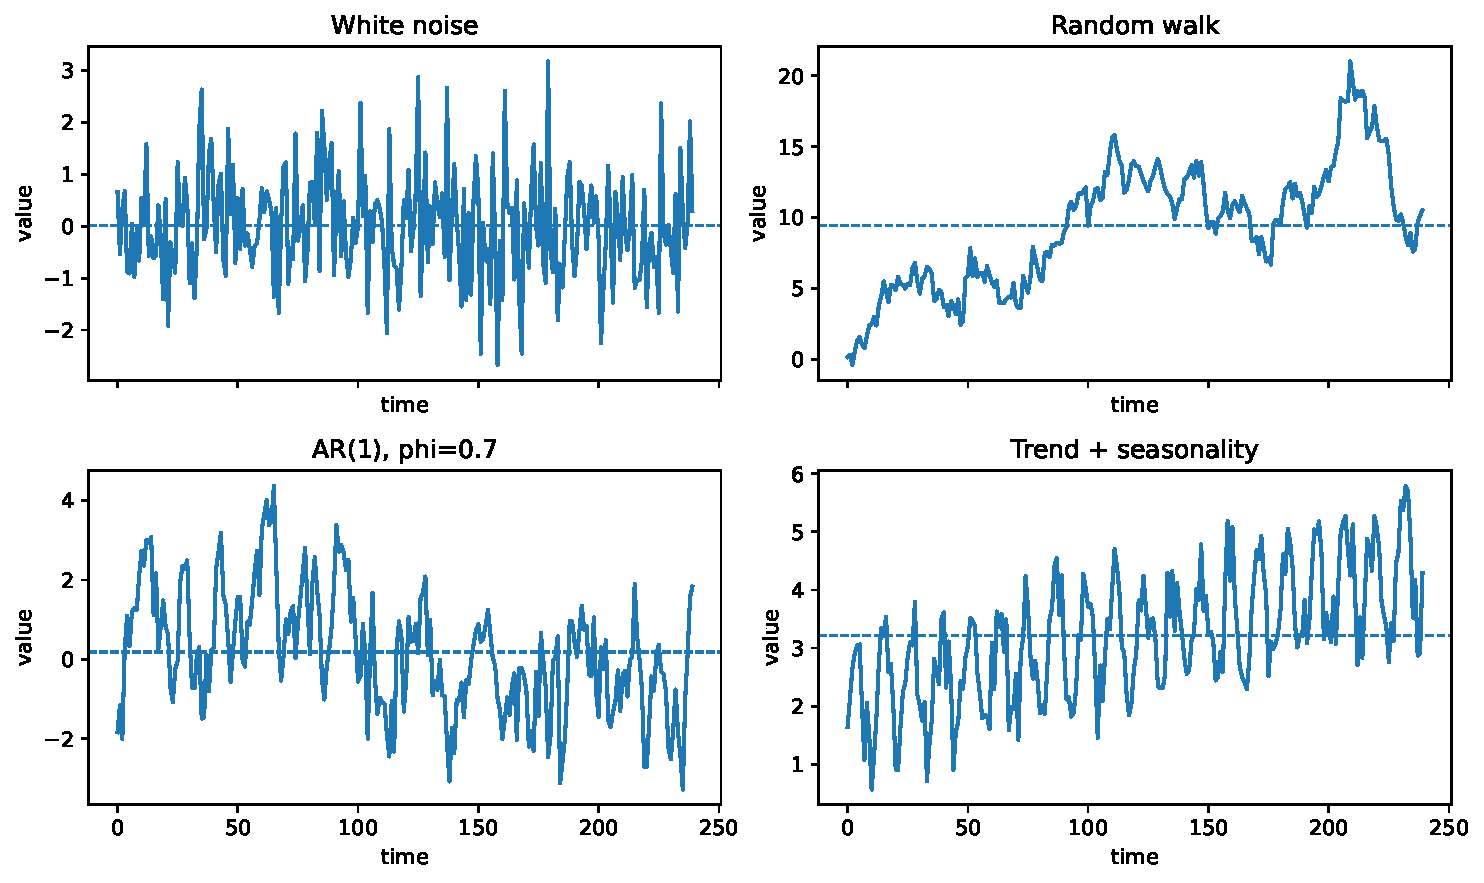
\includegraphics[keepaspectratio]{chapters/chapter-01-why-time-series-and-sequences_files/figure-pdf/ch01-four-processes-output-1.pdf}}

\begin{tcolorbox}[enhanced jigsaw, arc=.35mm, bottomrule=.15mm, bottomtitle=1mm, breakable, colback=white, colbacktitle=quarto-callout-note-color!10!white, colframe=quarto-callout-note-color-frame, coltitle=black, left=2mm, leftrule=.75mm, opacityback=0, opacitybacktitle=0.6, rightrule=.15mm, title=\textcolor{quarto-callout-note-color}{\faInfo}\hspace{0.5em}{What to notice}, titlerule=0mm, toprule=.15mm, toptitle=1mm]

A random walk may look like a trend even when its increments have mean
zero. This is one reason that visual trend detection must be paired with
mathematical diagnostics.

\end{tcolorbox}

\section{1.9 Python example: empirical mean and variance over
time}\label{python-example-empirical-mean-and-variance-over-time}

For a random walk \(S_t=\sum_{i=1}^t W_i\), theory says \(E[S_t]=0\) and
\(\operatorname{Var}(S_t)=t\sigma^2\). We can check this by simulating
many paths.

\begin{Shaded}
\begin{Highlighting}[]
\NormalTok{n\_paths }\OperatorTok{=} \DecValTok{2000}
\NormalTok{n\_steps }\OperatorTok{=} \DecValTok{150}
\NormalTok{sigma }\OperatorTok{=} \FloatTok{1.0}
\NormalTok{walks }\OperatorTok{=}\NormalTok{ np.vstack([simulate\_random\_walk(n\_steps, sigma}\OperatorTok{=}\NormalTok{sigma, rng}\OperatorTok{=}\NormalTok{rng) }\ControlFlowTok{for}\NormalTok{ \_ }\KeywordTok{in} \BuiltInTok{range}\NormalTok{(n\_paths)])}

\NormalTok{empirical\_mean }\OperatorTok{=}\NormalTok{ walks.mean(axis}\OperatorTok{=}\DecValTok{0}\NormalTok{)}
\NormalTok{empirical\_var }\OperatorTok{=}\NormalTok{ walks.var(axis}\OperatorTok{=}\DecValTok{0}\NormalTok{)}
\NormalTok{t }\OperatorTok{=}\NormalTok{ np.arange(}\DecValTok{1}\NormalTok{, n\_steps }\OperatorTok{+} \DecValTok{1}\NormalTok{)}

\NormalTok{df\_moments }\OperatorTok{=}\NormalTok{ pd.DataFrame(\{}
    \StringTok{"time"}\NormalTok{: t,}
    \StringTok{"empirical\_mean"}\NormalTok{: empirical\_mean,}
    \StringTok{"empirical\_variance"}\NormalTok{: empirical\_var,}
    \StringTok{"theoretical\_variance"}\NormalTok{: t }\OperatorTok{*}\NormalTok{ sigma}\OperatorTok{**}\DecValTok{2}\NormalTok{,}
\NormalTok{\})}

\NormalTok{df\_moments.head()}
\end{Highlighting}
\end{Shaded}

\protect\phantomsection\label{ch01-random-walk-moments}
{\def\LTcaptype{none} % do not increment counter
\begin{longtable}[]{@{}lllll@{}}
\toprule\noalign{}
& time & empirical\_mean & empirical\_variance &
theoretical\_variance \\
\midrule\noalign{}
\endhead
\bottomrule\noalign{}
\endlastfoot
0 & 1 & 0.022169 & 1.015279 & 1.0 \\
1 & 2 & -0.016335 & 2.007345 & 2.0 \\
2 & 3 & -0.028065 & 3.004240 & 3.0 \\
3 & 4 & -0.031805 & 4.059932 & 4.0 \\
4 & 5 & -0.041788 & 5.146741 & 5.0 \\
\end{longtable}
}

\begin{Shaded}
\begin{Highlighting}[]
\NormalTok{plt.figure(figsize}\OperatorTok{=}\NormalTok{(}\DecValTok{9}\NormalTok{, }\DecValTok{4}\NormalTok{))}
\NormalTok{plt.plot(df\_moments[}\StringTok{"time"}\NormalTok{], df\_moments[}\StringTok{"empirical\_variance"}\NormalTok{], label}\OperatorTok{=}\StringTok{"empirical variance"}\NormalTok{)}
\NormalTok{plt.plot(df\_moments[}\StringTok{"time"}\NormalTok{], df\_moments[}\StringTok{"theoretical\_variance"}\NormalTok{], linestyle}\OperatorTok{=}\StringTok{"{-}{-}"}\NormalTok{, label}\OperatorTok{=}\StringTok{"theoretical variance"}\NormalTok{)}
\NormalTok{plt.xlabel(}\StringTok{"time"}\NormalTok{)}
\NormalTok{plt.ylabel(}\StringTok{"variance across simulated paths"}\NormalTok{)}
\NormalTok{plt.title(}\StringTok{"Variance of a random walk grows linearly in time"}\NormalTok{)}
\NormalTok{plt.legend()}
\NormalTok{plt.show()}
\end{Highlighting}
\end{Shaded}

\pandocbounded{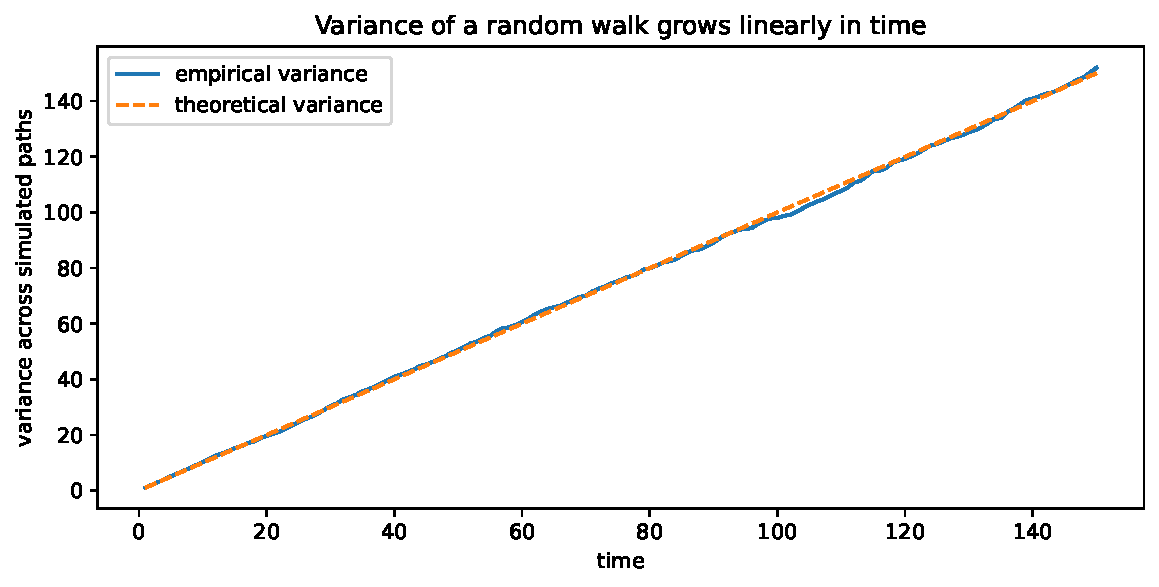
\includegraphics[keepaspectratio]{chapters/chapter-01-why-time-series-and-sequences_files/figure-pdf/ch01-random-walk-variance-plot-output-1.pdf}}

This growth of variance is an early warning sign of nonstationarity.
Later, we will formalize stationarity and use differencing to transform
some nonstationary processes into stationary ones.

\section{1.10 Python example: sequence windows for machine
learning}\label{python-example-sequence-windows-for-machine-learning}

Deep-learning models usually do not ingest a full scalar time series as
a single object. We first create windows. For a lookback length \(L\)
and horizon \(h\), define

\[
X^{(i)} = (x_i,x_{i+1},\dots,x_{i+L-1}),
\]

and

\[
y^{(i)} = x_{i+L+h-1}.
\]

This converts one sequence into a supervised-learning data set.

\begin{Shaded}
\begin{Highlighting}[]
\KeywordTok{def}\NormalTok{ make\_windows(x, lookback}\OperatorTok{=}\DecValTok{24}\NormalTok{, horizon}\OperatorTok{=}\DecValTok{1}\NormalTok{):}
\NormalTok{    x }\OperatorTok{=}\NormalTok{ np.asarray(x, dtype}\OperatorTok{=}\BuiltInTok{float}\NormalTok{)}
\NormalTok{    X, y }\OperatorTok{=}\NormalTok{ [], []}
\NormalTok{    last\_start }\OperatorTok{=} \BuiltInTok{len}\NormalTok{(x) }\OperatorTok{{-}}\NormalTok{ lookback }\OperatorTok{{-}}\NormalTok{ horizon }\OperatorTok{+} \DecValTok{1}
    \ControlFlowTok{for}\NormalTok{ start }\KeywordTok{in} \BuiltInTok{range}\NormalTok{(last\_start):}
\NormalTok{        X.append(x[start:start }\OperatorTok{+}\NormalTok{ lookback])}
\NormalTok{        y.append(x[start }\OperatorTok{+}\NormalTok{ lookback }\OperatorTok{+}\NormalTok{ horizon }\OperatorTok{{-}} \DecValTok{1}\NormalTok{])}
    \ControlFlowTok{return}\NormalTok{ np.array(X), np.array(y)}

\NormalTok{x }\OperatorTok{=}\NormalTok{ simulate\_trend\_seasonal(n}\OperatorTok{=}\DecValTok{300}\NormalTok{, period}\OperatorTok{=}\DecValTok{24}\NormalTok{)}
\NormalTok{X, y }\OperatorTok{=}\NormalTok{ make\_windows(x, lookback}\OperatorTok{=}\DecValTok{24}\NormalTok{, horizon}\OperatorTok{=}\DecValTok{1}\NormalTok{)}

\NormalTok{X.shape, y.shape}
\end{Highlighting}
\end{Shaded}

\protect\phantomsection\label{ch01-window-function}
\begin{verbatim}
((276, 24), (276,))
\end{verbatim}

\begin{Shaded}
\begin{Highlighting}[]
\NormalTok{lookback }\OperatorTok{=} \DecValTok{24}
\NormalTok{horizon }\OperatorTok{=} \DecValTok{1}
\NormalTok{start }\OperatorTok{=} \DecValTok{60}

\NormalTok{plt.figure(figsize}\OperatorTok{=}\NormalTok{(}\DecValTok{10}\NormalTok{, }\DecValTok{4}\NormalTok{))}
\NormalTok{plt.plot(x, linewidth}\OperatorTok{=}\DecValTok{1}\NormalTok{)}
\NormalTok{plt.scatter(np.arange(start, start }\OperatorTok{+}\NormalTok{ lookback), x[start:start }\OperatorTok{+}\NormalTok{ lookback], label}\OperatorTok{=}\StringTok{"input window"}\NormalTok{)}
\NormalTok{plt.scatter([start }\OperatorTok{+}\NormalTok{ lookback }\OperatorTok{+}\NormalTok{ horizon }\OperatorTok{{-}} \DecValTok{1}\NormalTok{], [x[start }\OperatorTok{+}\NormalTok{ lookback }\OperatorTok{+}\NormalTok{ horizon }\OperatorTok{{-}} \DecValTok{1}\NormalTok{]], marker}\OperatorTok{=}\StringTok{"x"}\NormalTok{, s}\OperatorTok{=}\DecValTok{80}\NormalTok{, label}\OperatorTok{=}\StringTok{"target"}\NormalTok{)}
\NormalTok{plt.axvspan(start, start }\OperatorTok{+}\NormalTok{ lookback }\OperatorTok{{-}} \DecValTok{1}\NormalTok{, alpha}\OperatorTok{=}\FloatTok{0.15}\NormalTok{)}
\NormalTok{plt.title(}\StringTok{"A time series becomes supervised learning through sliding windows"}\NormalTok{)}
\NormalTok{plt.xlabel(}\StringTok{"time"}\NormalTok{)}
\NormalTok{plt.ylabel(}\StringTok{"value"}\NormalTok{)}
\NormalTok{plt.legend()}
\NormalTok{plt.show()}
\end{Highlighting}
\end{Shaded}

\pandocbounded{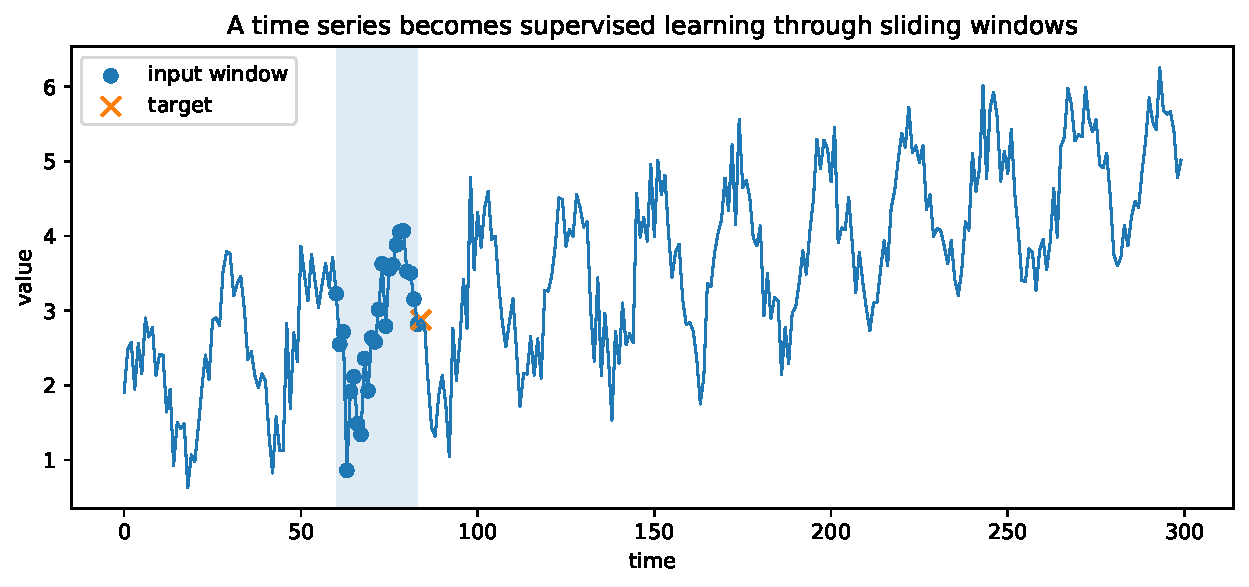
\includegraphics[keepaspectratio]{chapters/chapter-01-why-time-series-and-sequences_files/figure-pdf/ch01-window-visualization-output-1.pdf}}

\begin{tcolorbox}[enhanced jigsaw, arc=.35mm, bottomrule=.15mm, bottomtitle=1mm, breakable, colback=white, colbacktitle=quarto-callout-important-color!10!white, colframe=quarto-callout-important-color-frame, coltitle=black, left=2mm, leftrule=.75mm, opacityback=0, opacitybacktitle=0.6, rightrule=.15mm, title=\textcolor{quarto-callout-important-color}{\faExclamation}\hspace{0.5em}{Windowing does not remove dependence}, titlerule=0mm, toprule=.15mm, toptitle=1mm]

The rows of the windowed matrix \(X\) are highly overlapping. Treating
them as independent rows can mislead uncertainty estimates and
validation results. The validation split still needs to respect time
order.

\end{tcolorbox}

\section{1.11 A first baseline
forecast}\label{a-first-baseline-forecast}

Before using ARIMA, Prophet, LSTM, or transformers, always build simple
baselines. Two basic baselines are:

\begin{enumerate}
\def\labelenumi{\arabic{enumi}.}
\tightlist
\item
  \textbf{Naive forecast:} \(\widehat x_{t+1}=x_t\).
\item
  \textbf{Mean forecast:} \(\widehat x_{t+1}=\bar x_{1:t}\).
\end{enumerate}

For many real data sets, a sophisticated model is not useful unless it
beats these simple baselines under a time-aware validation scheme.

\begin{Shaded}
\begin{Highlighting}[]
\NormalTok{x }\OperatorTok{=}\NormalTok{ simulate\_ar1(n}\OperatorTok{=}\DecValTok{260}\NormalTok{, phi}\OperatorTok{=}\FloatTok{0.8}\NormalTok{)}
\NormalTok{train\_size }\OperatorTok{=} \DecValTok{200}
\NormalTok{train }\OperatorTok{=}\NormalTok{ x[:train\_size]}
\NormalTok{test }\OperatorTok{=}\NormalTok{ x[train\_size:]}

\CommentTok{\# One{-}step naive forecast on the test period: previous observed value.}
\NormalTok{naive\_forecast }\OperatorTok{=}\NormalTok{ x[train\_size}\OperatorTok{{-}}\DecValTok{1}\NormalTok{:}\OperatorTok{{-}}\DecValTok{1}\NormalTok{]}

\CommentTok{\# Expanding mean forecast.}
\NormalTok{history }\OperatorTok{=} \BuiltInTok{list}\NormalTok{(train)}
\NormalTok{mean\_forecast }\OperatorTok{=}\NormalTok{ []}
\ControlFlowTok{for}\NormalTok{ obs }\KeywordTok{in}\NormalTok{ test:}
\NormalTok{    mean\_forecast.append(np.mean(history))}
\NormalTok{    history.append(obs)}
\NormalTok{mean\_forecast }\OperatorTok{=}\NormalTok{ np.array(mean\_forecast)}

\KeywordTok{def}\NormalTok{ rmse(actual, pred):}
    \ControlFlowTok{return} \BuiltInTok{float}\NormalTok{(np.sqrt(np.mean((actual }\OperatorTok{{-}}\NormalTok{ pred)}\OperatorTok{**}\DecValTok{2}\NormalTok{)))}

\BuiltInTok{print}\NormalTok{(}\StringTok{"Naive RMSE:"}\NormalTok{, rmse(test, naive\_forecast))}
\BuiltInTok{print}\NormalTok{(}\StringTok{"Mean  RMSE:"}\NormalTok{, rmse(test, mean\_forecast))}

\NormalTok{plt.figure(figsize}\OperatorTok{=}\NormalTok{(}\DecValTok{10}\NormalTok{, }\DecValTok{4}\NormalTok{))}
\NormalTok{plt.plot(np.arange(train\_size), train, label}\OperatorTok{=}\StringTok{"train"}\NormalTok{)}
\NormalTok{plt.plot(np.arange(train\_size, }\BuiltInTok{len}\NormalTok{(x)), test, label}\OperatorTok{=}\StringTok{"test"}\NormalTok{)}
\NormalTok{plt.plot(np.arange(train\_size, }\BuiltInTok{len}\NormalTok{(x)), naive\_forecast, linestyle}\OperatorTok{=}\StringTok{"{-}{-}"}\NormalTok{, label}\OperatorTok{=}\StringTok{"naive forecast"}\NormalTok{)}
\NormalTok{plt.plot(np.arange(train\_size, }\BuiltInTok{len}\NormalTok{(x)), mean\_forecast, linestyle}\OperatorTok{=}\StringTok{":"}\NormalTok{, label}\OperatorTok{=}\StringTok{"expanding mean forecast"}\NormalTok{)}
\NormalTok{plt.xlabel(}\StringTok{"time"}\NormalTok{)}
\NormalTok{plt.ylabel(}\StringTok{"value"}\NormalTok{)}
\NormalTok{plt.title(}\StringTok{"Time{-}aware train/test split and baseline forecasts"}\NormalTok{)}
\NormalTok{plt.legend()}
\NormalTok{plt.show()}
\end{Highlighting}
\end{Shaded}

\begin{verbatim}
Naive RMSE: 1.0941083318954319
Mean  RMSE: 1.6574298880036455
\end{verbatim}

\pandocbounded{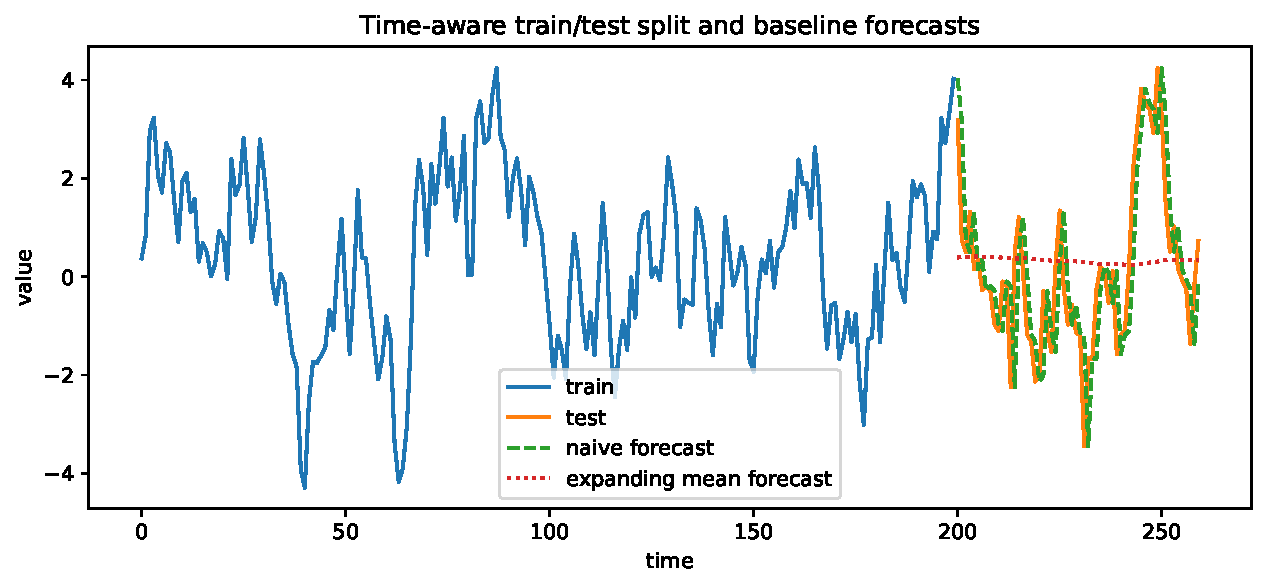
\includegraphics[keepaspectratio]{chapters/chapter-01-why-time-series-and-sequences_files/figure-pdf/ch01-baseline-forecast-output-2.pdf}}

\section{1.12 AI-assisted study: use AI as a model
critic}\label{ai-assisted-study-use-ai-as-a-model-critic}

AI tools are useful in this course, but only when the interaction is
structured. For time series, a generic request such as ``forecast this
data'' is usually too vague. A better request forces the assistant to
state assumptions and diagnostics.

\section{AI-assisted modeling prompt}\label{ai-assisted-modeling-prompt}

Use the following prompt after you have a time plot and basic summary
statistics.

\begin{quote}
I have a univariate time series observed at equally spaced times. I need
to forecast the next \(h\) values. First, list plausible data-generating
structures: white noise, random walk, trend-plus-noise, seasonality,
ARMA dependence, changing variance, or regime switching. For each
structure, tell me one visual diagnostic, one mathematical assumption,
one simple baseline forecast, and one way the model could fail. Do not
choose a final model until I provide a time plot, ACF, validation
design, and residual diagnostics.
\end{quote}

\begin{tcolorbox}[enhanced jigsaw, arc=.35mm, bottomrule=.15mm, bottomtitle=1mm, breakable, colback=white, colbacktitle=quarto-callout-warning-color!10!white, colframe=quarto-callout-warning-color-frame, coltitle=black, left=2mm, leftrule=.75mm, opacityback=0, opacitybacktitle=0.6, rightrule=.15mm, title=\textcolor{quarto-callout-warning-color}{\faExclamationTriangle}\hspace{0.5em}{What not to outsource}, titlerule=0mm, toprule=.15mm, toptitle=1mm]

Do not let AI decide the validation design without checking it. Do not
accept a model only because it gives code. In this class, every
AI-generated suggestion must be checked against mathematical assumptions
and out-of-sample performance.

\end{tcolorbox}

\section{1.13 Mathematical summary}\label{mathematical-summary}

Here are the core objects from the chapter.

{\def\LTcaptype{none} % do not increment counter
\begin{longtable}[]{@{}
  >{\raggedright\arraybackslash}p{(\linewidth - 4\tabcolsep) * \real{0.3000}}
  >{\raggedleft\arraybackslash}p{(\linewidth - 4\tabcolsep) * \real{0.4000}}
  >{\raggedright\arraybackslash}p{(\linewidth - 4\tabcolsep) * \real{0.3000}}@{}}
\toprule\noalign{}
\begin{minipage}[b]{\linewidth}\raggedright
Concept
\end{minipage} & \begin{minipage}[b]{\linewidth}\raggedleft
Mathematical form
\end{minipage} & \begin{minipage}[b]{\linewidth}\raggedright
Interpretation
\end{minipage} \\
\midrule\noalign{}
\endhead
\bottomrule\noalign{}
\endlastfoot
Stochastic process & \(\{X_t:t\in T\}\) & Random variables indexed by
time or order \\
Realization & \(x_1,\dots,x_n\) & One observed sample path \\
Mean function & \(\mu_t=E[X_t]\) & Average level at time \(t\) \\
Covariance function & \(\gamma(s,t)=\operatorname{Cov}(X_s,X_t)\) &
Linear dependence between two times \\
White noise & \(W_t\sim WN(0,\sigma^2)\) & Uncorrelated zero-mean
shocks \\
Random walk & \(S_t=S_{t-1}+W_t\) & Accumulated shocks; nonstationary
level \\
Difference & \(\nabla S_t=S_t-S_{t-1}\) & Change from one time to the
next \\
Forecast & \(\widehat X_{n+h|n}=E[X_{n+h}\mid X_1,\dots,X_n]\) & Best
mean-square prediction under the model \\
Windowed input & \((x_{t-L+1},\dots,x_t)\) & Sequence input for ML
models \\
\end{longtable}
}

\section{1.14 Common mistakes}\label{common-mistakes}

\begin{enumerate}
\def\labelenumi{\arabic{enumi}.}
\tightlist
\item
  \textbf{Ignoring order.} A time series is not a bag of observations.
\item
  \textbf{Using random splits for forecasting.} This leaks future
  information.
\item
  \textbf{Confusing uncorrelated with independent.} White noise is
  uncorrelated; i.i.d. noise is stronger.
\item
  \textbf{Calling every upward path a deterministic trend.} A random
  walk can visually drift.
\item
  \textbf{Using a deep model before a baseline.} A neural model should
  be compared against naive, seasonal naive, and simple statistical
  models.
\item
  \textbf{Trusting a forecast without uncertainty.} Forecasts need error
  measures and, when possible, prediction intervals.
\item
  \textbf{Asking AI for answers instead of assumptions.} Use AI to
  generate hypotheses and checks, not as a substitute for diagnostics.
\end{enumerate}

\section{1.15 Exercises}\label{exercises}

\subsection{Conceptual exercises}\label{conceptual-exercises}

\begin{enumerate}
\def\labelenumi{\arabic{enumi}.}
\tightlist
\item
  Explain the difference between a stochastic process and a realization.
\item
  Give one example of discrete-time continuous-state data and one
  example of discrete-time discrete-state data.
\item
  Why is i.i.d. white noise usually uninteresting for forecasting future
  values?
\item
  Let \(S_t=\sum_{i=1}^t W_i\), where \(W_i\) are independent with mean
  \(0\) and variance \(\sigma^2\). Derive \(E[S_t]\) and
  \(\operatorname{Var}(S_t)\).
\item
  Suppose \(X_t=\beta_0+\beta_1t+E_t\). Compute
  \(\nabla X_t=X_t-X_{t-1}\).
\end{enumerate}

\subsection{Computational exercises}\label{computational-exercises}

\begin{enumerate}
\def\labelenumi{\arabic{enumi}.}
\tightlist
\item
  Simulate 100 realizations of white noise and 100 realizations of a
  random walk. Compare the distribution of \(X_{100}\) in both cases.
\item
  Write your own function to compute the first difference of a sequence.
\item
  Create a time-aware train/test split for a simulated AR(1) series.
  Compare naive and mean forecasts.
\item
  Use the windowing function to create input-output pairs for lookback
  lengths \(L=6,12,24\). How does the number of training examples
  change?
\item
  Create a trend-plus-seasonal sequence. Try a random train-test split
  and a time-ordered split. Explain why the random split is misleading.
\end{enumerate}

\subsection{AI-assisted exercise}\label{ai-assisted-exercise}

Ask an AI assistant to propose three possible models for a simulated
series from this chapter. Then write a verification report with four
parts:

\begin{enumerate}
\def\labelenumi{\arabic{enumi}.}
\tightlist
\item
  the AI's proposed model;
\item
  the assumption behind that model;
\item
  the diagnostic plot or statistic you used to check the assumption;
\item
  whether you accept, reject, or modify the suggestion.
\end{enumerate}

\section{1.16 Chapter checklist}\label{chapter-checklist}

Before moving to Chapter 2, make sure you can do the following without
notes:

\begin{itemize}
\tightlist
\item
  define \(\{X_t\}\) and \(\{x_t\}\);
\item
  explain why dependence matters for forecasting;
\item
  simulate white noise and a random walk;
\item
  derive the variance of a random walk;
\item
  create supervised-learning windows from a sequence;
\item
  explain why random splitting is usually inappropriate for forecasting;
\item
  write an AI prompt that asks for assumptions and diagnostics.
\end{itemize}

\section{Further reading}\label{further-reading}

Classical notation and introductory examples are covered in {[}1{]} and
{[}2{]}. Forecasting validation and baseline thinking are developed in
{[}3{]}. Later chapters connect these ideas to neural sequence modeling
and modern AI systems.

\chapter{Exploratory Data Analysis for Time
Series}\label{exploratory-data-analysis-for-time-series}

\textbf{Part I. Time Series as Dependent Data}\\
\textbf{Chapter goal:} learn how to turn a raw ordered sequence into
mathematical hypotheses, diagnostic plots, transformed series, and
reproducible modeling decisions before fitting ARMA, ARIMA, Prophet, or
neural sequence models.

\section{Learning objectives}\label{learning-objectives-1}

After studying this chapter, you should be able to:

\begin{enumerate}
\def\labelenumi{\arabic{enumi}.}
\tightlist
\item
  explain why exploratory data analysis for time series is different
  from EDA for independent tabular data;
\item
  decompose a series into trend, seasonal, cyclic, and residual
  components;
\item
  use transformations, detrending, differencing, seasonal differencing,
  and smoothing to reveal dependence structure;
\item
  compute and interpret rolling summaries, lag plots, sample
  autocovariance, and sample autocorrelation;
\item
  connect visual patterns to candidate mathematical models such as
  trend-plus-stationary-noise, random walk, seasonal ARIMA, and
  nonlinear sequence models;
\item
  implement a complete EDA workflow in Python using reproducible code;
\item
  use AI tools as hypothesis generators and diagnostic critics, not as
  black-box model selectors.
\end{enumerate}

\section{2.1 Why EDA comes before
modeling}\label{why-eda-comes-before-modeling}

A time series is one observed path

\[
x_1,x_2,\dots,x_n
\]

from an underlying stochastic process

\[
\{X_t:t\in T\}.
\]

Before fitting a model, we need to ask what kind of structure is visible
in the sample path. In ordinary tabular machine learning, exploratory
analysis often focuses on distributions of columns, missing values,
pairwise scatterplots, and correlations among features. For time series,
order is central. A histogram of the values may be useful, but it does
not show whether large values cluster in time, whether the mean changes,
whether variance grows, whether there is seasonality, or whether the
series contains abrupt regime changes.

A practical time-series EDA workflow asks questions such as:

\begin{itemize}
\tightlist
\item
  Is the level roughly constant, or does it drift over time?
\item
  Does variability appear constant, or does the variance increase with
  the level?
\item
  Are there repeating seasonal patterns?
\item
  Are there outliers, missing blocks, or structural breaks?
\item
  Does the current value depend on previous values?
\item
  Is the dependence short-range, long-range, seasonal, nonlinear, or
  regime-dependent?
\item
  What simple baseline forecast should every advanced model beat?
\end{itemize}

EDA is therefore not separate from theory. It is the first step in
choosing a mathematical model.

\begin{tcolorbox}[enhanced jigsaw, arc=.35mm, bottomrule=.15mm, bottomtitle=1mm, breakable, colback=white, colbacktitle=quarto-callout-note-color!10!white, colframe=quarto-callout-note-color-frame, coltitle=black, left=2mm, leftrule=.75mm, opacityback=0, opacitybacktitle=0.6, rightrule=.15mm, title=\textcolor{quarto-callout-note-color}{\faInfo}\hspace{0.5em}{Guiding principle}, titlerule=0mm, toprule=.15mm, toptitle=1mm]

Exploratory analysis should not merely produce attractive plots. It
should produce \textbf{candidate assumptions}. Each plot should help
answer: what model class is plausible, and what model class is probably
inappropriate?

\end{tcolorbox}

\section{2.2 The basic decomposition
model}\label{the-basic-decomposition-model}

A useful starting point is the additive decomposition

\[
X_t = \mu_t + Y_t,
\]

where \(\mu_t\) is a deterministic mean structure and \(Y_t\) is a
zero-mean stochastic component. The deterministic component may include
trend and seasonality:

\[
\mu_t = T_t + S_t.
\]

Thus,

\[
X_t = T_t + S_t + Y_t.
\]

A common parametric version is

\[
X_t = \beta_0 + \beta_1 t
+ \sum_{j=1}^m \left[a_j\cos(2\pi\omega_j t)+b_j\sin(2\pi\omega_j t)\right]
+Y_t.
\]

Here:

\begin{itemize}
\tightlist
\item
  \(\beta_0+\beta_1t\) represents a linear trend;
\item
  the sine and cosine terms represent periodic structure;
\item
  \(Y_t\) represents the residual time-dependent process.
\end{itemize}

The purpose of EDA is to decide whether a model like this is plausible
and, if so, how to estimate or remove \(T_t\) and \(S_t\) so that the
remaining component behaves more like a stationary process.

\begin{tcolorbox}[enhanced jigsaw, arc=.35mm, bottomrule=.15mm, bottomtitle=1mm, breakable, colback=white, colbacktitle=quarto-callout-important-color!10!white, colframe=quarto-callout-important-color-frame, coltitle=black, left=2mm, leftrule=.75mm, opacityback=0, opacitybacktitle=0.6, rightrule=.15mm, title=\textcolor{quarto-callout-important-color}{\faExclamation}\hspace{0.5em}{Deterministic structure versus stochastic dependence}, titlerule=0mm, toprule=.15mm, toptitle=1mm]

A seasonal pattern can come from a deterministic mean function, from
stochastic dependence at seasonal lags, or from both. EDA helps separate
these possibilities, but final model choice requires residual
diagnostics and validation.

\end{tcolorbox}

\section{2.3 Additive and multiplicative
structure}\label{additive-and-multiplicative-structure}

The additive model

\[
X_t=T_t+S_t+Y_t
\]

works well when the seasonal amplitude and noise scale are roughly
constant over time.

Sometimes the seasonal amplitude grows with the level of the series.
Then a multiplicative decomposition may be more appropriate:

\[
X_t = T_t S_t E_t.
\]

If all values are positive, taking logarithms turns this into an
additive structure:

\[
\log X_t = \log T_t + \log S_t + \log E_t.
\]

This is the first example of a broader principle: transformations are
not cosmetic. They change the scale on which a model's assumptions are
supposed to hold.

\section{2.4 Time plots and rolling
summaries}\label{time-plots-and-rolling-summaries}

The first plot is usually the time plot:

\[
t \mapsto x_t.
\]

A time plot helps detect trend, seasonality, outliers, missing values,
and changes in variability. But a time plot alone is subjective, so it
is often paired with rolling summaries. For a window size \(m\), the
rolling mean is

\[
\widehat\mu_t^{(m)} = \frac{1}{m}\sum_{j=0}^{m-1}x_{t-j},
\]

and the rolling variance is

\[
\widehat\sigma_t^{2,(m)}
=\frac{1}{m-1}\sum_{j=0}^{m-1}\left(x_{t-j}-\widehat\mu_t^{(m)}\right)^2.
\]

If the rolling mean changes substantially, a stationary constant-mean
model may be inappropriate. If the rolling variance grows or shrinks
systematically, a variance-stabilizing transformation may be needed.

\begin{tcolorbox}[enhanced jigsaw, arc=.35mm, bottomrule=.15mm, bottomtitle=1mm, breakable, colback=white, colbacktitle=quarto-callout-tip-color!10!white, colframe=quarto-callout-tip-color-frame, coltitle=black, left=2mm, leftrule=.75mm, opacityback=0, opacitybacktitle=0.6, rightrule=.15mm, title=\textcolor{quarto-callout-tip-color}{\faLightbulb}\hspace{0.5em}{What to look for in the first plot}, titlerule=0mm, toprule=.15mm, toptitle=1mm]

A slowly changing center suggests trend. Repeated peaks and valleys
suggest seasonality. Bursts of volatility suggest nonconstant variance.
A sudden jump suggests a structural break or intervention. Isolated
extreme values suggest outliers or data-quality issues.

\end{tcolorbox}

\section{2.5 Transformations and variance
stabilization}\label{transformations-and-variance-stabilization}

A transformation is often used when variability depends on the level.
Common transformations include:

\[
Z_t = \log(X_t), \qquad X_t>0,
\]

\[
Z_t = \sqrt{X_t}, \qquad X_t\ge 0,
\]

and the Box-Cox family

\[
Z_t^{(\lambda)} =
\begin{cases}
\dfrac{X_t^\lambda-1}{\lambda}, & \lambda\ne 0,\\[6pt]
\log X_t, & \lambda=0.
\end{cases}
\]

Transformations should be chosen based on the scientific meaning of the
data as well as diagnostic behavior. For example, a log transform is
natural for growth data because differences on the log scale approximate
relative changes:

\[
\log X_t-\log X_{t-1}=\log\left(\frac{X_t}{X_{t-1}}\right).
\]

For financial prices, this motivates log returns.

\section{2.6 Detrending by regression}\label{detrending-by-regression}

Suppose the observed series is

\[
X_t = \mu_t + Y_t,
\]

where \(Y_t\) is a zero-mean stationary process and \(\mu_t\) is a
deterministic trend. If the trend is linear, then

\[
\mu_t = \beta_0 + \beta_1 t.
\]

The regression model is

\[
x_t = \beta_0+\beta_1t+e_t.
\]

More generally, let

\[
z_t = \begin{bmatrix}1 & z_{t1} & z_{t2} & \cdots & z_{tq}\end{bmatrix}^T
\]

and

\[
x_t = z_t^T\beta + e_t.
\]

Stacking the observations gives

\[
x = Z\beta + e.
\]

The ordinary least-squares estimator is

\[
\widehat\beta=(Z^TZ)^{-1}Z^Tx,
\]

when \(Z^TZ\) is invertible. The fitted trend is

\[
\widehat\mu = Z\widehat\beta,
\]

and the detrended residuals are

\[
e_t = x_t-\widehat\mu_t.
\]

In time-series modeling, these residuals are not automatically
independent. The regression is used to estimate deterministic structure,
but the residuals must still be checked for autocorrelation.

\begin{tcolorbox}[enhanced jigsaw, arc=.35mm, bottomrule=.15mm, bottomtitle=1mm, breakable, colback=white, colbacktitle=quarto-callout-warning-color!10!white, colframe=quarto-callout-warning-color-frame, coltitle=black, left=2mm, leftrule=.75mm, opacityback=0, opacitybacktitle=0.6, rightrule=.15mm, title=\textcolor{quarto-callout-warning-color}{\faExclamationTriangle}\hspace{0.5em}{Regression assumptions are often violated}, titlerule=0mm, toprule=.15mm, toptitle=1mm]

Classical regression inference assumes independent errors. Time-series
residuals often remain correlated. The fitted trend may still be useful,
but standard errors and \(p\)-values from ordinary regression can be
misleading unless dependence is addressed.

\end{tcolorbox}

\section{2.7 Seasonal regression with Fourier
features}\label{seasonal-regression-with-fourier-features}

A deterministic seasonal component with period \(s\) can be represented
using sine and cosine terms. For one harmonic,

\[
S_t=a\cos\left(\frac{2\pi t}{s}\right)+b\sin\left(\frac{2\pi t}{s}\right).
\]

For \(K\) harmonics,

\[
S_t=\sum_{k=1}^K\left[a_k\cos\left(\frac{2\pi kt}{s}\right)+b_k\sin\left(\frac{2\pi kt}{s}\right)\right].
\]

This lets us fit seasonality using linear regression, because the
unknown parameters are the coefficients \(a_k\) and \(b_k\), not the
nonlinear phase directly.

This idea connects three parts of the course:

\begin{enumerate}
\def\labelenumi{\arabic{enumi}.}
\tightlist
\item
  exploratory seasonal regression in this chapter;
\item
  spectral analysis and Fourier transforms later;
\item
  Prophet-style additive models and Fourier seasonal features in
  automated forecasting.
\end{enumerate}

\section{2.8 Differencing}\label{differencing}

Another way to remove trend is differencing. The first difference is

\[
\nabla x_t = x_t-x_{t-1}.
\]

Using the backshift operator \(B\), defined by

\[
Bx_t=x_{t-1},
\]

we can write

\[
\nabla = 1-B.
\]

The second difference is

\[
\nabla^2x_t = \nabla(\nabla x_t)
= x_t-2x_{t-1}+x_{t-2}.
\]

In general,

\[
\nabla^d=(1-B)^d.
\]

Differencing removes polynomial trends. If \(x_t\) contains a
deterministic polynomial trend of degree \(d\), then the \(d\)-th
difference removes that trend up to a constant.

For example, if

\[
x_t=\beta_0+\beta_1t+y_t,
\]

then

\[
\nabla x_t = \beta_1 + y_t-y_{t-1}.
\]

The intercept \(\beta_0\) is removed and the slope becomes the mean
level of the differenced series.

\section{2.9 Seasonal differencing}\label{seasonal-differencing}

For seasonal data with period \(s\), the seasonal difference is

\[
\nabla_s x_t = x_t-x_{t-s}=(1-B^s)x_t.
\]

For monthly data with yearly seasonality, \(s=12\). For hourly data with
daily seasonality, \(s=24\). Seasonal differencing removes repeated
seasonal levels when the same season in adjacent cycles is comparable.

A model may use both ordinary and seasonal differencing:

\[
(1-B)^d(1-B^s)^D X_t.
\]

This expression appears later in SARIMA models.

\section{2.10 Detrending versus
differencing}\label{detrending-versus-differencing}

Detrending and differencing are not the same operation.

\subsection{Detrending}\label{detrending}

If

\[
x_t=\mu_t+y_t,
\]

then detrending estimates \(\mu_t\) and studies

\[
e_t=x_t-\widehat\mu_t.
\]

This attempts to preserve the stochastic component \(y_t\).

\subsection{Differencing}\label{differencing-1}

Differencing forms

\[
\nabla x_t=\nabla\mu_t+\nabla y_t.
\]

This can remove the trend, but it also changes the stochastic component.
For example, if \(y_t\) is white noise, then

\[
\nabla y_t = y_t-y_{t-1}
\]

is no longer white noise. It has negative lag-one autocorrelation.

\begin{tcolorbox}[enhanced jigsaw, arc=.35mm, bottomrule=.15mm, bottomtitle=1mm, breakable, colback=white, colbacktitle=quarto-callout-important-color!10!white, colframe=quarto-callout-important-color-frame, coltitle=black, left=2mm, leftrule=.75mm, opacityback=0, opacitybacktitle=0.6, rightrule=.15mm, title=\textcolor{quarto-callout-important-color}{\faExclamation}\hspace{0.5em}{Differencing can create dependence}, titlerule=0mm, toprule=.15mm, toptitle=1mm]

Differencing is powerful, but over-differencing can introduce artificial
dependence. Use time plots, ACF/PACF, residual diagnostics, and forecast
validation to decide how much differencing is appropriate.

\end{tcolorbox}

\section{2.11 Smoothing as filtering}\label{smoothing-as-filtering}

Smoothing reduces short-term noise to reveal slower structure. A simple
moving average smoother is

\[
\widetilde x_t = \frac{1}{m}\sum_{j=0}^{m-1}x_{t-j}.
\]

More generally, a linear smoother is a filter

\[
\widetilde x_t=\sum_j a_j x_{t-j}.
\]

Smoothing is useful for visualization, but it should be used carefully.
A smoothed curve is not the original data. It can blur abrupt changes,
shift peaks, and create edge effects.

Exponential smoothing uses recursively decaying weights:

\[
\ell_t = \alpha x_t+(1-\alpha)\ell_{t-1}, \qquad 0<\alpha<1.
\]

Large \(\alpha\) reacts quickly to new observations; small \(\alpha\)
produces stronger smoothing.

\section{2.12 Lag plots and
autocorrelation}\label{lag-plots-and-autocorrelation}

A lag plot compares \(x_t\) with \(x_{t-h}\) for a fixed lag \(h\). If
the points show a strong linear pattern, then the series has dependence
at lag \(h\).

For a zero-mean stationary process, the autocovariance at lag \(h\) is

\[
\gamma(h)=\operatorname{Cov}(X_t,X_{t-h}).
\]

The autocorrelation is

\[
\rho(h)=\frac{\gamma(h)}{\gamma(0)}.
\]

Given data \(x_1,\dots,x_n\), the sample mean is

\[
\bar x = \frac{1}{n}\sum_{t=1}^n x_t,
\]

and a common sample autocovariance estimate is

\[
\widehat\gamma(h)=\frac{1}{n}\sum_{t=h+1}^n (x_t-\bar x)(x_{t-h}-\bar x).
\]

The sample autocorrelation is

\[
\widehat\rho(h)=\frac{\widehat\gamma(h)}{\widehat\gamma(0)}.
\]

The ACF plot is one of the most important EDA tools in classical
time-series analysis. A slowly decaying ACF often suggests
nonstationarity or trend. Spikes at seasonal lags suggest seasonal
dependence. A sharp cutoff after lag \(q\) may suggest an MA(\(q\))
model, while a geometrically decaying pattern may suggest an AR model.

\section{2.13 A practical EDA decision
map}\label{a-practical-eda-decision-map}

The following table summarizes common patterns and possible next steps.

{\def\LTcaptype{none} % do not increment counter
\begin{longtable}[]{@{}
  >{\raggedright\arraybackslash}p{(\linewidth - 4\tabcolsep) * \real{0.3333}}
  >{\raggedright\arraybackslash}p{(\linewidth - 4\tabcolsep) * \real{0.3333}}
  >{\raggedright\arraybackslash}p{(\linewidth - 4\tabcolsep) * \real{0.3333}}@{}}
\toprule\noalign{}
\begin{minipage}[b]{\linewidth}\raggedright
Observed pattern
\end{minipage} & \begin{minipage}[b]{\linewidth}\raggedright
Possible interpretation
\end{minipage} & \begin{minipage}[b]{\linewidth}\raggedright
Useful next step
\end{minipage} \\
\midrule\noalign{}
\endhead
\bottomrule\noalign{}
\endlastfoot
Changing mean & Trend, drift, intervention, regime change & Detrend,
difference, or use state-space trend model \\
Increasing variance & Multiplicative noise, growth scale & Try log or
Box-Cox transform \\
Repeated pattern every \(s\) periods & Seasonality & Seasonal plot,
Fourier features, seasonal differencing \\
Slow ACF decay & Trend, random walk, long memory & Difference, detrend,
test stationarity \\
Significant ACF at lag \(s,2s,3s\) & Seasonal dependence & SARIMA or
seasonal features \\
Outliers & Data error, rare event, intervention & Flag, explain, robust
model, intervention variable \\
Abrupt level shift & Change point, new regime & Segment data or use
regime-switching/state-space model \\
Nonlinear lag structure & Nonlinear dynamics & Feature ML, tree models,
neural sequence models \\
\end{longtable}
}

\begin{tcolorbox}[enhanced jigsaw, arc=.35mm, bottomrule=.15mm, bottomtitle=1mm, breakable, colback=white, colbacktitle=quarto-callout-tip-color!10!white, colframe=quarto-callout-tip-color-frame, coltitle=black, left=2mm, leftrule=.75mm, opacityback=0, opacitybacktitle=0.6, rightrule=.15mm, title=\textcolor{quarto-callout-tip-color}{\faLightbulb}\hspace{0.5em}{EDA output}, titlerule=0mm, toprule=.15mm, toptitle=1mm]

At the end of EDA, you should be able to write a paragraph such as:
``The raw series has a rising level and yearly seasonality. A log
transform stabilizes variance. After first and seasonal differencing,
the ACF decays quickly but has a remaining lag-one spike. I will compare
seasonal naive, SARIMA, and an ML model with Fourier and lag features.''

\end{tcolorbox}

\section{2.14 Interactive demonstration: trend, seasonality, smoothing,
and
differencing}\label{interactive-demonstration-trend-seasonality-smoothing-and-differencing}

Use the interactive below to create synthetic data with trend and
seasonality. Then compare the raw series, a moving-average smoother, a
fitted trend, and differenced versions.

\begin{tcolorbox}[enhanced jigsaw, arc=.35mm, bottomrule=.15mm, bottomtitle=1mm, breakable, colback=white, colbacktitle=quarto-callout-tip-color!10!white, colframe=quarto-callout-tip-color-frame, coltitle=black, left=2mm, leftrule=.75mm, opacityback=0, opacitybacktitle=0.6, rightrule=.15mm, title=\textcolor{quarto-callout-tip-color}{\faLightbulb}\hspace{0.5em}{How to use this widget}, titlerule=0mm, toprule=.15mm, toptitle=1mm]

Increase the trend slope and watch the ACF decay more slowly. Increase
seasonal amplitude and look for repeating structure. Increase the
smoothing window to reveal trend, but notice that smoothing does not
create a stationary series. Compare first differencing and seasonal
differencing.

\end{tcolorbox}

Trend slope Seasonal amplitude Period Noise scale Smoothing window
Transformation None Log after positive shift View Raw + smoother +
fitted trend Detrended residual First difference Seasonal difference

\protect\phantomsection\label{ch02_eda_plot}

\protect\phantomsection\label{ch02_eda_acf}

Plotly.js is loaded once globally from assets/header.html. This chapter
does not include another Plotly script tag.

\section{2.15 Python example: simulate a series for
EDA}\label{python-example-simulate-a-series-for-eda}

We first create a synthetic series with trend, seasonality, and
correlated residual noise. The goal is not only to plot it, but to
recover the structure through EDA.

\begin{Shaded}
\begin{Highlighting}[]
\ImportTok{import}\NormalTok{ numpy }\ImportTok{as}\NormalTok{ np}
\ImportTok{import}\NormalTok{ pandas }\ImportTok{as}\NormalTok{ pd}
\ImportTok{import}\NormalTok{ matplotlib.pyplot }\ImportTok{as}\NormalTok{ plt}

\NormalTok{rng }\OperatorTok{=}\NormalTok{ np.random.default\_rng(}\DecValTok{7339}\NormalTok{)}


\KeywordTok{def}\NormalTok{ simulate\_eda\_series(n}\OperatorTok{=}\DecValTok{240}\NormalTok{, period}\OperatorTok{=}\DecValTok{24}\NormalTok{, beta0}\OperatorTok{=}\FloatTok{5.0}\NormalTok{, beta1}\OperatorTok{=}\FloatTok{0.025}\NormalTok{,}
\NormalTok{                        amplitude}\OperatorTok{=}\FloatTok{2.0}\NormalTok{, phi}\OperatorTok{=}\FloatTok{0.55}\NormalTok{, sigma}\OperatorTok{=}\FloatTok{0.7}\NormalTok{, rng}\OperatorTok{=}\NormalTok{rng):}
    \CommentTok{"""Trend + seasonal mean + AR(1){-}type residual noise."""}
\NormalTok{    t }\OperatorTok{=}\NormalTok{ np.arange(n)}
\NormalTok{    trend }\OperatorTok{=}\NormalTok{ beta0 }\OperatorTok{+}\NormalTok{ beta1 }\OperatorTok{*}\NormalTok{ t}
\NormalTok{    seasonal }\OperatorTok{=}\NormalTok{ amplitude }\OperatorTok{*}\NormalTok{ np.sin(}\DecValTok{2} \OperatorTok{*}\NormalTok{ np.pi }\OperatorTok{*}\NormalTok{ t }\OperatorTok{/}\NormalTok{ period) }\OperatorTok{+} \FloatTok{0.5} \OperatorTok{*}\NormalTok{ amplitude }\OperatorTok{*}\NormalTok{ np.cos(}\DecValTok{4} \OperatorTok{*}\NormalTok{ np.pi }\OperatorTok{*}\NormalTok{ t }\OperatorTok{/}\NormalTok{ period)}

\NormalTok{    w }\OperatorTok{=}\NormalTok{ rng.normal(}\FloatTok{0.0}\NormalTok{, sigma, size}\OperatorTok{=}\NormalTok{n)}
\NormalTok{    y }\OperatorTok{=}\NormalTok{ np.zeros(n)}
    \ControlFlowTok{for}\NormalTok{ i }\KeywordTok{in} \BuiltInTok{range}\NormalTok{(}\DecValTok{1}\NormalTok{, n):}
\NormalTok{        y[i] }\OperatorTok{=}\NormalTok{ phi }\OperatorTok{*}\NormalTok{ y[i}\OperatorTok{{-}}\DecValTok{1}\NormalTok{] }\OperatorTok{+}\NormalTok{ w[i]}

\NormalTok{    x }\OperatorTok{=}\NormalTok{ trend }\OperatorTok{+}\NormalTok{ seasonal }\OperatorTok{+}\NormalTok{ y}
    \ControlFlowTok{return}\NormalTok{ pd.DataFrame(\{}
        \StringTok{"time"}\NormalTok{: t,}
        \StringTok{"x"}\NormalTok{: x,}
        \StringTok{"trend"}\NormalTok{: trend,}
        \StringTok{"seasonal"}\NormalTok{: seasonal,}
        \StringTok{"residual\_process"}\NormalTok{: y,}
\NormalTok{    \})}


\NormalTok{df }\OperatorTok{=}\NormalTok{ simulate\_eda\_series()}
\NormalTok{df.head()}
\end{Highlighting}
\end{Shaded}

\protect\phantomsection\label{ch02-simulate-series}
{\def\LTcaptype{none} % do not increment counter
\begin{longtable}[]{@{}llllll@{}}
\toprule\noalign{}
& time & x & trend & seasonal & residual\_process \\
\midrule\noalign{}
\endhead
\bottomrule\noalign{}
\endlastfoot
0 & 0 & 6.000000 & 5.000 & 1.000000 & 0.000000 \\
1 & 1 & 6.036158 & 5.025 & 1.383663 & -0.372505 \\
2 & 2 & 6.571969 & 5.050 & 1.500000 & 0.021969 \\
3 & 3 & 6.976047 & 5.075 & 1.414214 & 0.486834 \\
4 & 4 & 5.991593 & 5.100 & 1.232051 & -0.340458 \\
\end{longtable}
}

\begin{Shaded}
\begin{Highlighting}[]
\NormalTok{plt.figure(figsize}\OperatorTok{=}\NormalTok{(}\DecValTok{10}\NormalTok{, }\DecValTok{4}\NormalTok{))}
\NormalTok{plt.plot(df[}\StringTok{"time"}\NormalTok{], df[}\StringTok{"x"}\NormalTok{], linewidth}\OperatorTok{=}\DecValTok{1}\NormalTok{)}
\NormalTok{plt.xlabel(}\StringTok{"time"}\NormalTok{)}
\NormalTok{plt.ylabel(}\StringTok{"value"}\NormalTok{)}
\NormalTok{plt.title(}\StringTok{"Raw time plot"}\NormalTok{)}
\NormalTok{plt.show()}
\end{Highlighting}
\end{Shaded}

\pandocbounded{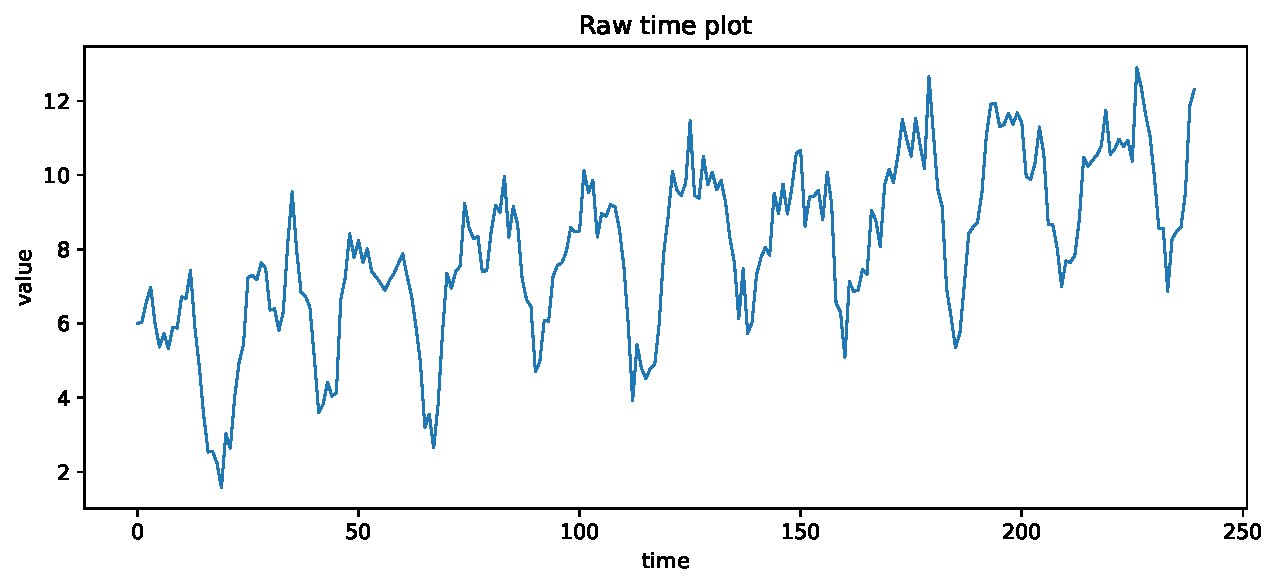
\includegraphics[keepaspectratio]{chapters/chapter-02-exploratory-data-analysis_files/figure-pdf/ch02-time-plot-output-1.pdf}}

The visible pattern suggests a deterministic component. We should not
immediately fit an ARMA model to the raw data because ARMA models assume
stationarity.

\section{2.16 Python example: rolling mean and rolling
variance}\label{python-example-rolling-mean-and-rolling-variance}

Rolling summaries provide a more stable view of time-varying level and
scale.

\begin{Shaded}
\begin{Highlighting}[]
\NormalTok{window }\OperatorTok{=} \DecValTok{24}
\NormalTok{roll\_mean }\OperatorTok{=}\NormalTok{ df[}\StringTok{"x"}\NormalTok{].rolling(window}\OperatorTok{=}\NormalTok{window, min\_periods}\OperatorTok{=}\DecValTok{1}\NormalTok{).mean()}
\NormalTok{roll\_std }\OperatorTok{=}\NormalTok{ df[}\StringTok{"x"}\NormalTok{].rolling(window}\OperatorTok{=}\NormalTok{window, min\_periods}\OperatorTok{=}\DecValTok{2}\NormalTok{).std()}

\NormalTok{fig, axes }\OperatorTok{=}\NormalTok{ plt.subplots(}\DecValTok{2}\NormalTok{, }\DecValTok{1}\NormalTok{, figsize}\OperatorTok{=}\NormalTok{(}\DecValTok{10}\NormalTok{, }\DecValTok{6}\NormalTok{), sharex}\OperatorTok{=}\VariableTok{True}\NormalTok{)}
\NormalTok{axes[}\DecValTok{0}\NormalTok{].plot(df[}\StringTok{"time"}\NormalTok{], df[}\StringTok{"x"}\NormalTok{], linewidth}\OperatorTok{=}\FloatTok{0.8}\NormalTok{, label}\OperatorTok{=}\StringTok{"series"}\NormalTok{)}
\NormalTok{axes[}\DecValTok{0}\NormalTok{].plot(df[}\StringTok{"time"}\NormalTok{], roll\_mean, linewidth}\OperatorTok{=}\DecValTok{2}\NormalTok{, label}\OperatorTok{=}\SpecialStringTok{f"rolling mean, m=}\SpecialCharTok{\{}\NormalTok{window}\SpecialCharTok{\}}\SpecialStringTok{"}\NormalTok{)}
\NormalTok{axes[}\DecValTok{0}\NormalTok{].set\_ylabel(}\StringTok{"value"}\NormalTok{)}
\NormalTok{axes[}\DecValTok{0}\NormalTok{].set\_title(}\StringTok{"Rolling mean"}\NormalTok{)}
\NormalTok{axes[}\DecValTok{0}\NormalTok{].legend()}

\NormalTok{axes[}\DecValTok{1}\NormalTok{].plot(df[}\StringTok{"time"}\NormalTok{], roll\_std, linewidth}\OperatorTok{=}\DecValTok{2}\NormalTok{)}
\NormalTok{axes[}\DecValTok{1}\NormalTok{].set\_xlabel(}\StringTok{"time"}\NormalTok{)}
\NormalTok{axes[}\DecValTok{1}\NormalTok{].set\_ylabel(}\StringTok{"rolling std"}\NormalTok{)}
\NormalTok{axes[}\DecValTok{1}\NormalTok{].set\_title(}\StringTok{"Rolling standard deviation"}\NormalTok{)}

\NormalTok{plt.tight\_layout()}
\NormalTok{plt.show()}
\end{Highlighting}
\end{Shaded}

\pandocbounded{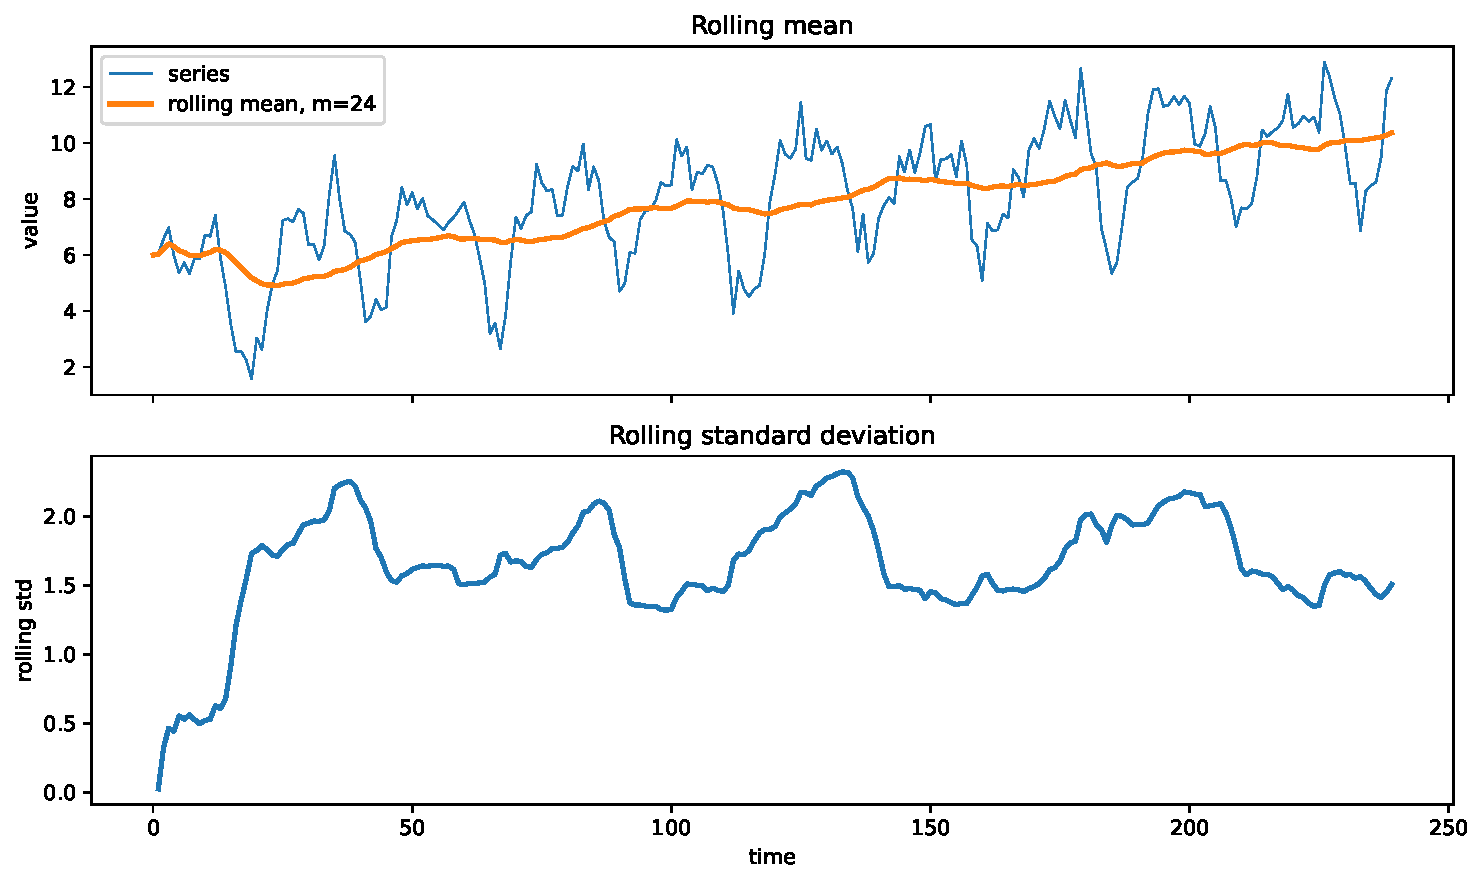
\includegraphics[keepaspectratio]{chapters/chapter-02-exploratory-data-analysis_files/figure-pdf/ch02-rolling-summary-output-1.pdf}}

\begin{tcolorbox}[enhanced jigsaw, arc=.35mm, bottomrule=.15mm, bottomtitle=1mm, breakable, colback=white, colbacktitle=quarto-callout-note-color!10!white, colframe=quarto-callout-note-color-frame, coltitle=black, left=2mm, leftrule=.75mm, opacityback=0, opacitybacktitle=0.6, rightrule=.15mm, title=\textcolor{quarto-callout-note-color}{\faInfo}\hspace{0.5em}{Interpretation}, titlerule=0mm, toprule=.15mm, toptitle=1mm]

The rolling mean is not a model by itself. It is a diagnostic smoother.
Its purpose is to help identify slow structure that should be modeled or
removed.

\end{tcolorbox}

\section{2.17 Python example: detrending with ordinary least
squares}\label{python-example-detrending-with-ordinary-least-squares}

We now fit the linear trend model

\[
x_t=\beta_0+\beta_1t+e_t.
\]

The code below computes the OLS estimator directly from the normal
equation.

\begin{Shaded}
\begin{Highlighting}[]
\NormalTok{x }\OperatorTok{=}\NormalTok{ df[}\StringTok{"x"}\NormalTok{].to\_numpy()}
\NormalTok{t }\OperatorTok{=}\NormalTok{ df[}\StringTok{"time"}\NormalTok{].to\_numpy()}

\NormalTok{Z }\OperatorTok{=}\NormalTok{ np.column\_stack([np.ones\_like(t), t])}
\NormalTok{beta\_hat }\OperatorTok{=}\NormalTok{ np.linalg.inv(Z.T }\OperatorTok{@}\NormalTok{ Z) }\OperatorTok{@}\NormalTok{ Z.T }\OperatorTok{@}\NormalTok{ x}
\NormalTok{fitted\_trend }\OperatorTok{=}\NormalTok{ Z }\OperatorTok{@}\NormalTok{ beta\_hat}
\NormalTok{residual\_linear }\OperatorTok{=}\NormalTok{ x }\OperatorTok{{-}}\NormalTok{ fitted\_trend}

\NormalTok{beta\_hat}
\end{Highlighting}
\end{Shaded}

\protect\phantomsection\label{ch02-ols-detrending}
\begin{verbatim}
array([5.39002345, 0.02174342])
\end{verbatim}

\begin{Shaded}
\begin{Highlighting}[]
\NormalTok{fig, axes }\OperatorTok{=}\NormalTok{ plt.subplots(}\DecValTok{2}\NormalTok{, }\DecValTok{1}\NormalTok{, figsize}\OperatorTok{=}\NormalTok{(}\DecValTok{10}\NormalTok{, }\DecValTok{6}\NormalTok{), sharex}\OperatorTok{=}\VariableTok{True}\NormalTok{)}
\NormalTok{axes[}\DecValTok{0}\NormalTok{].plot(t, x, linewidth}\OperatorTok{=}\DecValTok{1}\NormalTok{, label}\OperatorTok{=}\StringTok{"observed"}\NormalTok{)}
\NormalTok{axes[}\DecValTok{0}\NormalTok{].plot(t, fitted\_trend, linewidth}\OperatorTok{=}\DecValTok{2}\NormalTok{, label}\OperatorTok{=}\StringTok{"fitted linear trend"}\NormalTok{)}
\NormalTok{axes[}\DecValTok{0}\NormalTok{].set\_title(}\StringTok{"OLS trend fit"}\NormalTok{)}
\NormalTok{axes[}\DecValTok{0}\NormalTok{].set\_ylabel(}\StringTok{"value"}\NormalTok{)}
\NormalTok{axes[}\DecValTok{0}\NormalTok{].legend()}

\NormalTok{axes[}\DecValTok{1}\NormalTok{].plot(t, residual\_linear, linewidth}\OperatorTok{=}\DecValTok{1}\NormalTok{)}
\NormalTok{axes[}\DecValTok{1}\NormalTok{].axhline(}\DecValTok{0}\NormalTok{, linestyle}\OperatorTok{=}\StringTok{"{-}{-}"}\NormalTok{, linewidth}\OperatorTok{=}\DecValTok{1}\NormalTok{)}
\NormalTok{axes[}\DecValTok{1}\NormalTok{].set\_title(}\StringTok{"Residual after linear detrending"}\NormalTok{)}
\NormalTok{axes[}\DecValTok{1}\NormalTok{].set\_xlabel(}\StringTok{"time"}\NormalTok{)}
\NormalTok{axes[}\DecValTok{1}\NormalTok{].set\_ylabel(}\StringTok{"residual"}\NormalTok{)}

\NormalTok{plt.tight\_layout()}
\NormalTok{plt.show()}
\end{Highlighting}
\end{Shaded}

\pandocbounded{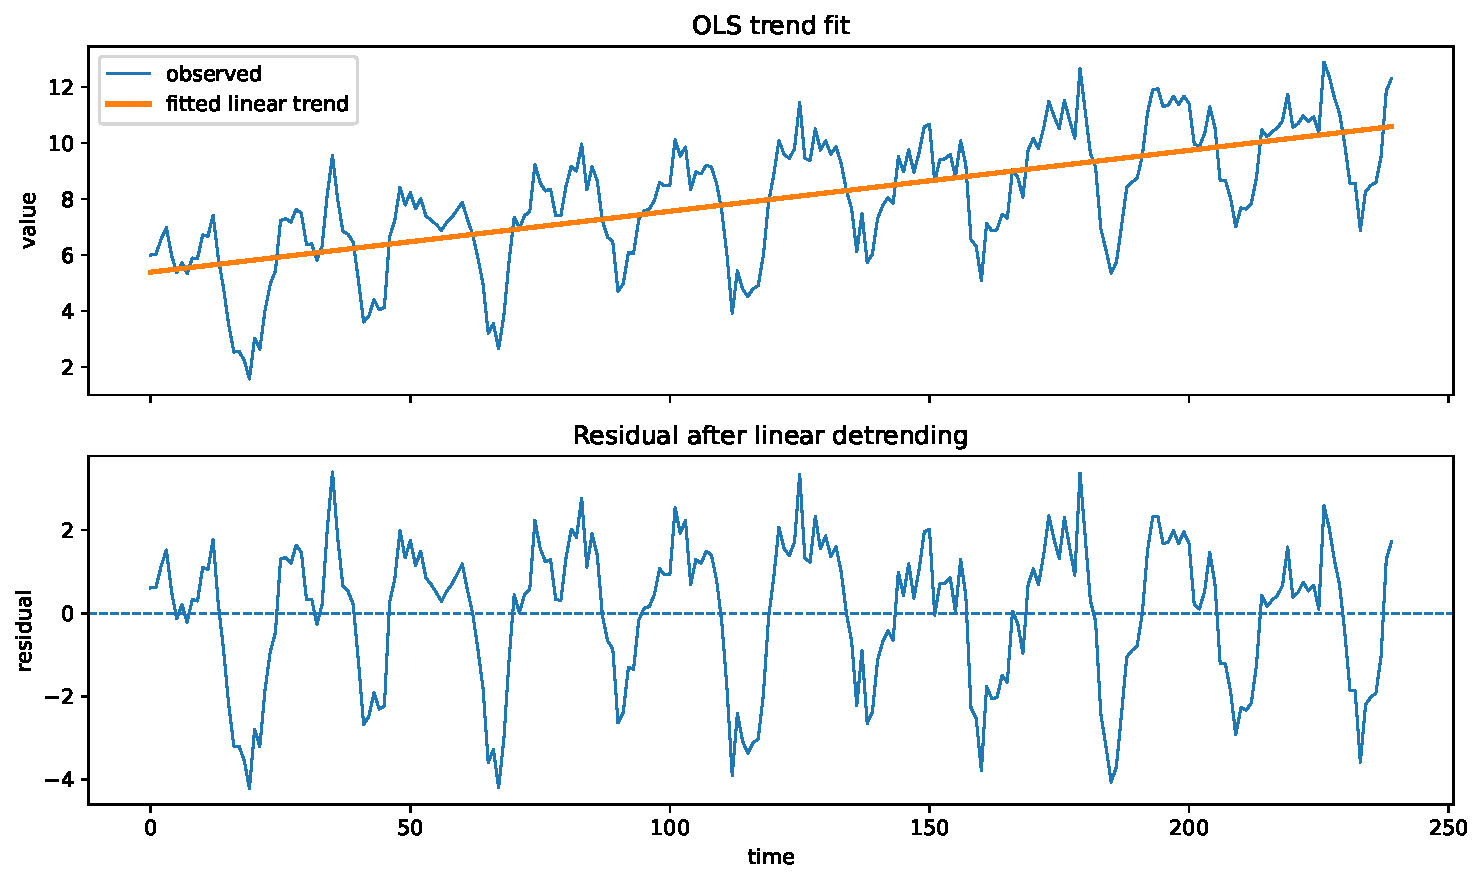
\includegraphics[keepaspectratio]{chapters/chapter-02-exploratory-data-analysis_files/figure-pdf/ch02-detrend-plot-output-1.pdf}}

The residual still has seasonal structure because we only removed a
linear trend. This is a common EDA discovery: removing one component may
reveal another.

\section{2.18 Python example: detrending and deseasonalizing with
Fourier
features}\label{python-example-detrending-and-deseasonalizing-with-fourier-features}

Now include Fourier features for a known period \(s=24\):

\[
x_t = \beta_0+\beta_1t+a_1\cos\left(\frac{2\pi t}{s}\right)
+b_1\sin\left(\frac{2\pi t}{s}\right)+e_t.
\]

We include two harmonics because the simulated data contains a second
harmonic.

\begin{Shaded}
\begin{Highlighting}[]
\NormalTok{period }\OperatorTok{=} \DecValTok{24}
\NormalTok{K }\OperatorTok{=} \DecValTok{2}
\NormalTok{cols }\OperatorTok{=}\NormalTok{ [np.ones\_like(t), t]}
\ControlFlowTok{for}\NormalTok{ k }\KeywordTok{in} \BuiltInTok{range}\NormalTok{(}\DecValTok{1}\NormalTok{, K }\OperatorTok{+} \DecValTok{1}\NormalTok{):}
\NormalTok{    cols.append(np.cos(}\DecValTok{2} \OperatorTok{*}\NormalTok{ np.pi }\OperatorTok{*}\NormalTok{ k }\OperatorTok{*}\NormalTok{ t }\OperatorTok{/}\NormalTok{ period))}
\NormalTok{    cols.append(np.sin(}\DecValTok{2} \OperatorTok{*}\NormalTok{ np.pi }\OperatorTok{*}\NormalTok{ k }\OperatorTok{*}\NormalTok{ t }\OperatorTok{/}\NormalTok{ period))}

\NormalTok{Z\_fourier }\OperatorTok{=}\NormalTok{ np.column\_stack(cols)}
\NormalTok{beta\_fourier }\OperatorTok{=}\NormalTok{ np.linalg.lstsq(Z\_fourier, x, rcond}\OperatorTok{=}\VariableTok{None}\NormalTok{)[}\DecValTok{0}\NormalTok{]}
\NormalTok{fitted\_mean }\OperatorTok{=}\NormalTok{ Z\_fourier }\OperatorTok{@}\NormalTok{ beta\_fourier}
\NormalTok{residual\_fourier }\OperatorTok{=}\NormalTok{ x }\OperatorTok{{-}}\NormalTok{ fitted\_mean}

\NormalTok{pd.Series(beta\_fourier, index}\OperatorTok{=}\NormalTok{[}\StringTok{"intercept"}\NormalTok{, }\StringTok{"time"}\NormalTok{, }\StringTok{"cos1"}\NormalTok{, }\StringTok{"sin1"}\NormalTok{, }\StringTok{"cos2"}\NormalTok{, }\StringTok{"sin2"}\NormalTok{])}
\end{Highlighting}
\end{Shaded}

\protect\phantomsection\label{ch02-fourier-regression}
\begin{verbatim}
intercept    5.194187
time         0.023382
cos1        -0.129335
sin1         1.916969
cos2         0.955717
sin2         0.092428
dtype: float64
\end{verbatim}

\begin{Shaded}
\begin{Highlighting}[]
\NormalTok{fig, axes }\OperatorTok{=}\NormalTok{ plt.subplots(}\DecValTok{2}\NormalTok{, }\DecValTok{1}\NormalTok{, figsize}\OperatorTok{=}\NormalTok{(}\DecValTok{10}\NormalTok{, }\DecValTok{6}\NormalTok{), sharex}\OperatorTok{=}\VariableTok{True}\NormalTok{)}
\NormalTok{axes[}\DecValTok{0}\NormalTok{].plot(t, x, linewidth}\OperatorTok{=}\DecValTok{1}\NormalTok{, label}\OperatorTok{=}\StringTok{"observed"}\NormalTok{)}
\NormalTok{axes[}\DecValTok{0}\NormalTok{].plot(t, fitted\_mean, linewidth}\OperatorTok{=}\DecValTok{2}\NormalTok{, label}\OperatorTok{=}\StringTok{"fitted trend + seasonality"}\NormalTok{)}
\NormalTok{axes[}\DecValTok{0}\NormalTok{].set\_title(}\StringTok{"Regression with trend and Fourier seasonal features"}\NormalTok{)}
\NormalTok{axes[}\DecValTok{0}\NormalTok{].set\_ylabel(}\StringTok{"value"}\NormalTok{)}
\NormalTok{axes[}\DecValTok{0}\NormalTok{].legend()}

\NormalTok{axes[}\DecValTok{1}\NormalTok{].plot(t, residual\_fourier, linewidth}\OperatorTok{=}\DecValTok{1}\NormalTok{)}
\NormalTok{axes[}\DecValTok{1}\NormalTok{].axhline(}\DecValTok{0}\NormalTok{, linestyle}\OperatorTok{=}\StringTok{"{-}{-}"}\NormalTok{, linewidth}\OperatorTok{=}\DecValTok{1}\NormalTok{)}
\NormalTok{axes[}\DecValTok{1}\NormalTok{].set\_title(}\StringTok{"Residual after detrending and deseasonalizing"}\NormalTok{)}
\NormalTok{axes[}\DecValTok{1}\NormalTok{].set\_xlabel(}\StringTok{"time"}\NormalTok{)}
\NormalTok{axes[}\DecValTok{1}\NormalTok{].set\_ylabel(}\StringTok{"residual"}\NormalTok{)}

\NormalTok{plt.tight\_layout()}
\NormalTok{plt.show()}
\end{Highlighting}
\end{Shaded}

\pandocbounded{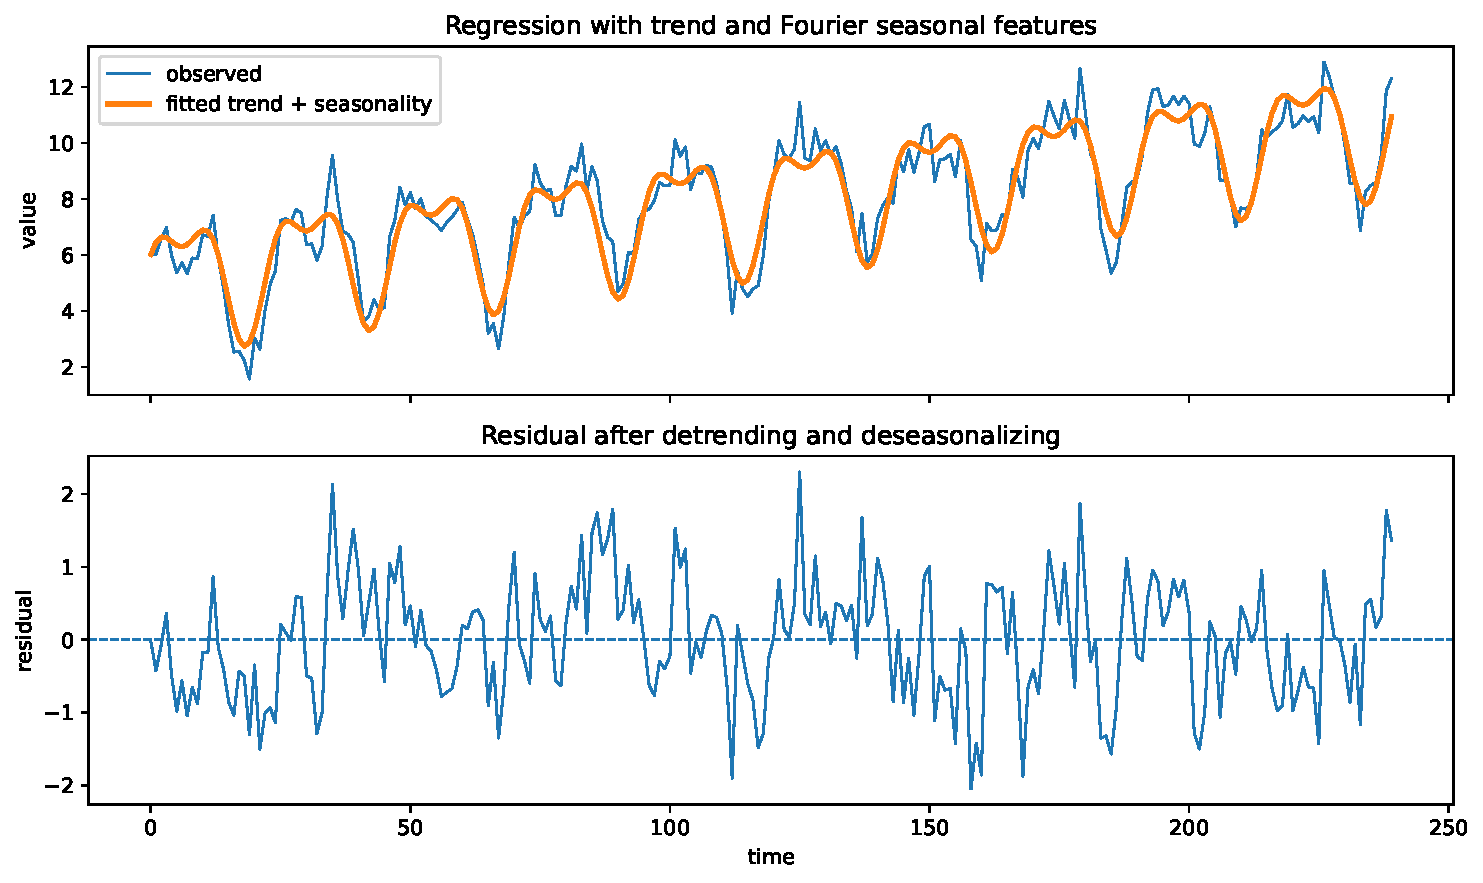
\includegraphics[keepaspectratio]{chapters/chapter-02-exploratory-data-analysis_files/figure-pdf/ch02-fourier-deseasonalize-plot-output-1.pdf}}

After removing deterministic trend and seasonality, the residual should
be checked for autocorrelation. If the residuals still have dependence,
we may model them with ARMA or another dependent-error model.

\section{2.19 Python example: sample ACF from
scratch}\label{python-example-sample-acf-from-scratch}

The sample ACF helps us see whether dependence remains after
transformation or detrending.

\protect\phantomsection\label{ch02-acf-function}
\begin{Shaded}
\begin{Highlighting}[]
\KeywordTok{def}\NormalTok{ sample\_acf(values, max\_lag}\OperatorTok{=}\DecValTok{40}\NormalTok{):}
\NormalTok{    values }\OperatorTok{=}\NormalTok{ np.asarray(values, dtype}\OperatorTok{=}\BuiltInTok{float}\NormalTok{)}
\NormalTok{    values }\OperatorTok{=}\NormalTok{ values }\OperatorTok{{-}}\NormalTok{ values.mean()}
\NormalTok{    denom }\OperatorTok{=}\NormalTok{ np.}\BuiltInTok{sum}\NormalTok{(values}\OperatorTok{**}\DecValTok{2}\NormalTok{)}
\NormalTok{    acf\_values }\OperatorTok{=}\NormalTok{ []}
    \ControlFlowTok{for}\NormalTok{ h }\KeywordTok{in} \BuiltInTok{range}\NormalTok{(max\_lag }\OperatorTok{+} \DecValTok{1}\NormalTok{):}
\NormalTok{        numer }\OperatorTok{=}\NormalTok{ np.}\BuiltInTok{sum}\NormalTok{(values[h:] }\OperatorTok{*}\NormalTok{ values[:}\BuiltInTok{len}\NormalTok{(values) }\OperatorTok{{-}}\NormalTok{ h])}
\NormalTok{        acf\_values.append(numer }\OperatorTok{/}\NormalTok{ denom)}
    \ControlFlowTok{return}\NormalTok{ np.array(acf\_values)}


\KeywordTok{def}\NormalTok{ plot\_acf\_stems(values, max\_lag}\OperatorTok{=}\DecValTok{40}\NormalTok{, title}\OperatorTok{=}\StringTok{"Sample ACF"}\NormalTok{):}
\NormalTok{    r }\OperatorTok{=}\NormalTok{ sample\_acf(values, max\_lag}\OperatorTok{=}\NormalTok{max\_lag)}
\NormalTok{    lags }\OperatorTok{=}\NormalTok{ np.arange(max\_lag }\OperatorTok{+} \DecValTok{1}\NormalTok{)}
\NormalTok{    bound }\OperatorTok{=} \FloatTok{1.96} \OperatorTok{/}\NormalTok{ np.sqrt(}\BuiltInTok{len}\NormalTok{(values))}
\NormalTok{    plt.figure(figsize}\OperatorTok{=}\NormalTok{(}\DecValTok{9}\NormalTok{, }\FloatTok{3.8}\NormalTok{))}
\NormalTok{    plt.axhline(}\DecValTok{0}\NormalTok{, linewidth}\OperatorTok{=}\DecValTok{1}\NormalTok{)}
\NormalTok{    plt.axhline(bound, linestyle}\OperatorTok{=}\StringTok{"{-}{-}"}\NormalTok{, linewidth}\OperatorTok{=}\DecValTok{1}\NormalTok{)}
\NormalTok{    plt.axhline(}\OperatorTok{{-}}\NormalTok{bound, linestyle}\OperatorTok{=}\StringTok{"{-}{-}"}\NormalTok{, linewidth}\OperatorTok{=}\DecValTok{1}\NormalTok{)}
\NormalTok{    plt.vlines(lags, }\DecValTok{0}\NormalTok{, r, linewidth}\OperatorTok{=}\DecValTok{1}\NormalTok{)}
\NormalTok{    plt.scatter(lags, r, s}\OperatorTok{=}\DecValTok{18}\NormalTok{)}
\NormalTok{    plt.xlabel(}\StringTok{"lag"}\NormalTok{)}
\NormalTok{    plt.ylabel(}\StringTok{"ACF"}\NormalTok{)}
\NormalTok{    plt.title(title)}
\NormalTok{    plt.ylim(}\OperatorTok{{-}}\DecValTok{1}\NormalTok{, }\DecValTok{1}\NormalTok{)}
\NormalTok{    plt.show()}

\NormalTok{plot\_acf\_stems(x, max\_lag}\OperatorTok{=}\DecValTok{60}\NormalTok{, title}\OperatorTok{=}\StringTok{"ACF of raw series"}\NormalTok{)}
\NormalTok{plot\_acf\_stems(residual\_fourier, max\_lag}\OperatorTok{=}\DecValTok{60}\NormalTok{, title}\OperatorTok{=}\StringTok{"ACF after trend + seasonal regression"}\NormalTok{)}
\end{Highlighting}
\end{Shaded}

\pandocbounded{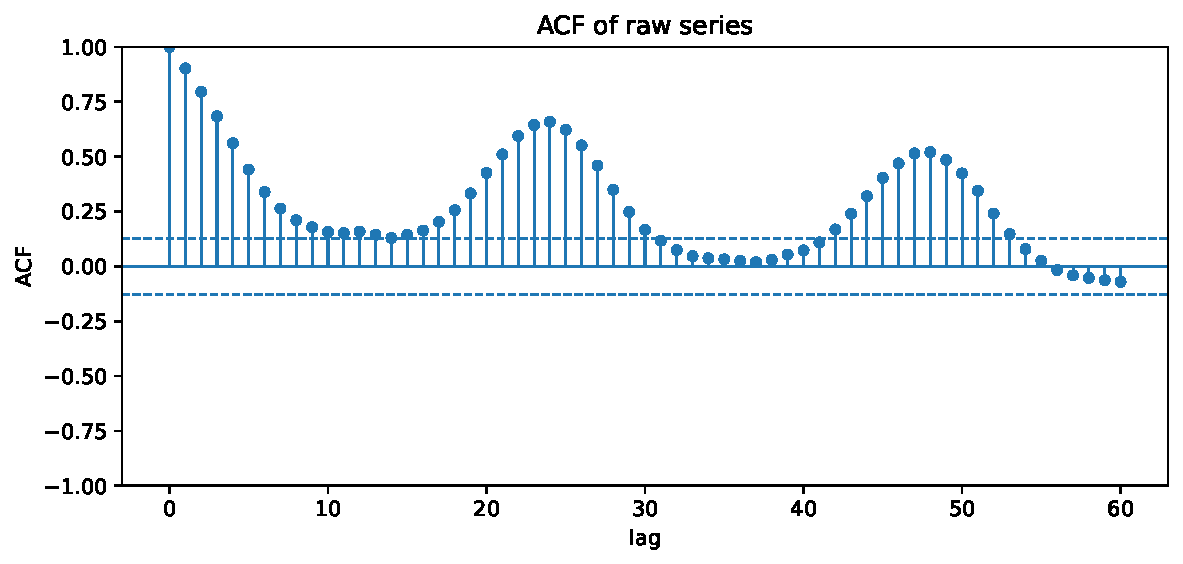
\includegraphics[keepaspectratio]{chapters/chapter-02-exploratory-data-analysis_files/figure-pdf/ch02-acf-function-output-1.pdf}}

\pandocbounded{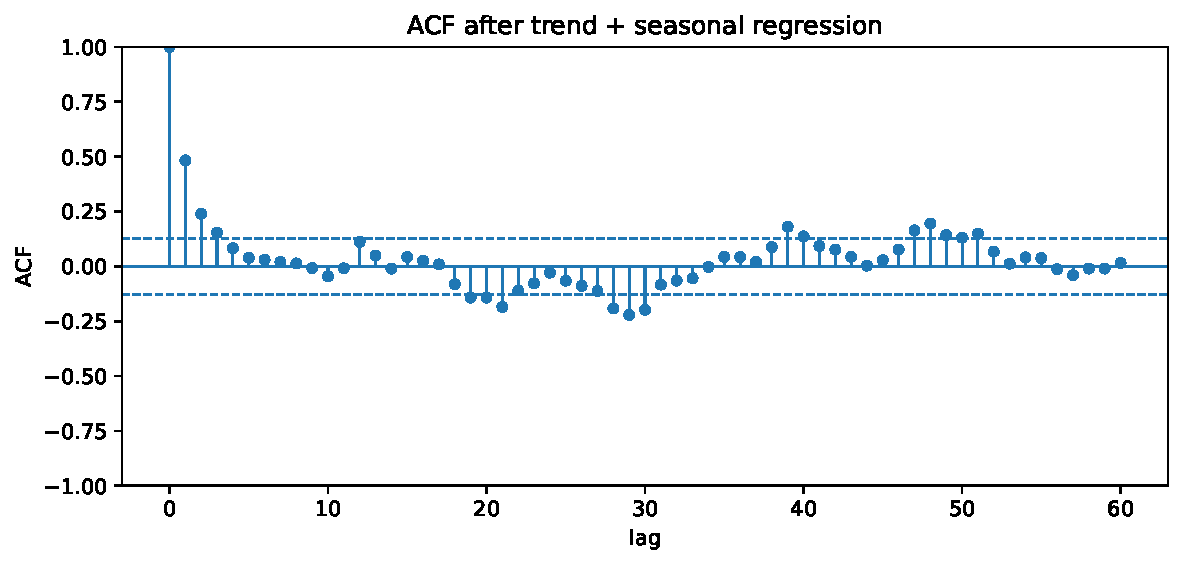
\includegraphics[keepaspectratio]{chapters/chapter-02-exploratory-data-analysis_files/figure-pdf/ch02-acf-function-output-2.pdf}}

\begin{tcolorbox}[enhanced jigsaw, arc=.35mm, bottomrule=.15mm, bottomtitle=1mm, breakable, colback=white, colbacktitle=quarto-callout-important-color!10!white, colframe=quarto-callout-important-color-frame, coltitle=black, left=2mm, leftrule=.75mm, opacityback=0, opacitybacktitle=0.6, rightrule=.15mm, title=\textcolor{quarto-callout-important-color}{\faExclamation}\hspace{0.5em}{Why the residual ACF matters}, titlerule=0mm, toprule=.15mm, toptitle=1mm]

A beautiful fitted trend curve does not mean the model is complete. If
residuals are autocorrelated, then there is still predictable structure
in the data.

\end{tcolorbox}

\section{2.20 Python example: differencing and seasonal
differencing}\label{python-example-differencing-and-seasonal-differencing}

Now compare first differencing and seasonal differencing.

\begin{Shaded}
\begin{Highlighting}[]
\KeywordTok{def}\NormalTok{ difference(values, lag}\OperatorTok{=}\DecValTok{1}\NormalTok{):}
\NormalTok{    values }\OperatorTok{=}\NormalTok{ np.asarray(values, dtype}\OperatorTok{=}\BuiltInTok{float}\NormalTok{)}
    \ControlFlowTok{return}\NormalTok{ values[lag:] }\OperatorTok{{-}}\NormalTok{ values[:}\OperatorTok{{-}}\NormalTok{lag]}

\NormalTok{first\_diff }\OperatorTok{=}\NormalTok{ difference(x, lag}\OperatorTok{=}\DecValTok{1}\NormalTok{)}
\NormalTok{seasonal\_diff }\OperatorTok{=}\NormalTok{ difference(x, lag}\OperatorTok{=}\NormalTok{period)}
\NormalTok{combined\_diff }\OperatorTok{=}\NormalTok{ difference(first\_diff, lag}\OperatorTok{=}\NormalTok{period)}

\BuiltInTok{len}\NormalTok{(x), }\BuiltInTok{len}\NormalTok{(first\_diff), }\BuiltInTok{len}\NormalTok{(seasonal\_diff), }\BuiltInTok{len}\NormalTok{(combined\_diff)}
\end{Highlighting}
\end{Shaded}

\protect\phantomsection\label{ch02-differencing-code}
\begin{verbatim}
(240, 239, 216, 215)
\end{verbatim}

\begin{Shaded}
\begin{Highlighting}[]
\NormalTok{fig, axes }\OperatorTok{=}\NormalTok{ plt.subplots(}\DecValTok{4}\NormalTok{, }\DecValTok{1}\NormalTok{, figsize}\OperatorTok{=}\NormalTok{(}\DecValTok{10}\NormalTok{, }\DecValTok{8}\NormalTok{), sharex}\OperatorTok{=}\VariableTok{False}\NormalTok{)}
\NormalTok{axes[}\DecValTok{0}\NormalTok{].plot(x, linewidth}\OperatorTok{=}\DecValTok{1}\NormalTok{)}
\NormalTok{axes[}\DecValTok{0}\NormalTok{].set\_title(}\StringTok{"Raw series"}\NormalTok{)}
\NormalTok{axes[}\DecValTok{1}\NormalTok{].plot(first\_diff, linewidth}\OperatorTok{=}\DecValTok{1}\NormalTok{)}
\NormalTok{axes[}\DecValTok{1}\NormalTok{].set\_title(}\StringTok{"First difference"}\NormalTok{)}
\NormalTok{axes[}\DecValTok{2}\NormalTok{].plot(seasonal\_diff, linewidth}\OperatorTok{=}\DecValTok{1}\NormalTok{)}
\NormalTok{axes[}\DecValTok{2}\NormalTok{].set\_title(}\SpecialStringTok{f"Seasonal difference, lag=}\SpecialCharTok{\{}\NormalTok{period}\SpecialCharTok{\}}\SpecialStringTok{"}\NormalTok{)}
\NormalTok{axes[}\DecValTok{3}\NormalTok{].plot(combined\_diff, linewidth}\OperatorTok{=}\DecValTok{1}\NormalTok{)}
\NormalTok{axes[}\DecValTok{3}\NormalTok{].set\_title(}\StringTok{"First difference followed by seasonal difference"}\NormalTok{)}
\ControlFlowTok{for}\NormalTok{ ax }\KeywordTok{in}\NormalTok{ axes:}
\NormalTok{    ax.axhline(}\DecValTok{0}\NormalTok{, linestyle}\OperatorTok{=}\StringTok{"{-}{-}"}\NormalTok{, linewidth}\OperatorTok{=}\DecValTok{1}\NormalTok{)}
\NormalTok{plt.tight\_layout()}
\NormalTok{plt.show()}
\end{Highlighting}
\end{Shaded}

\pandocbounded{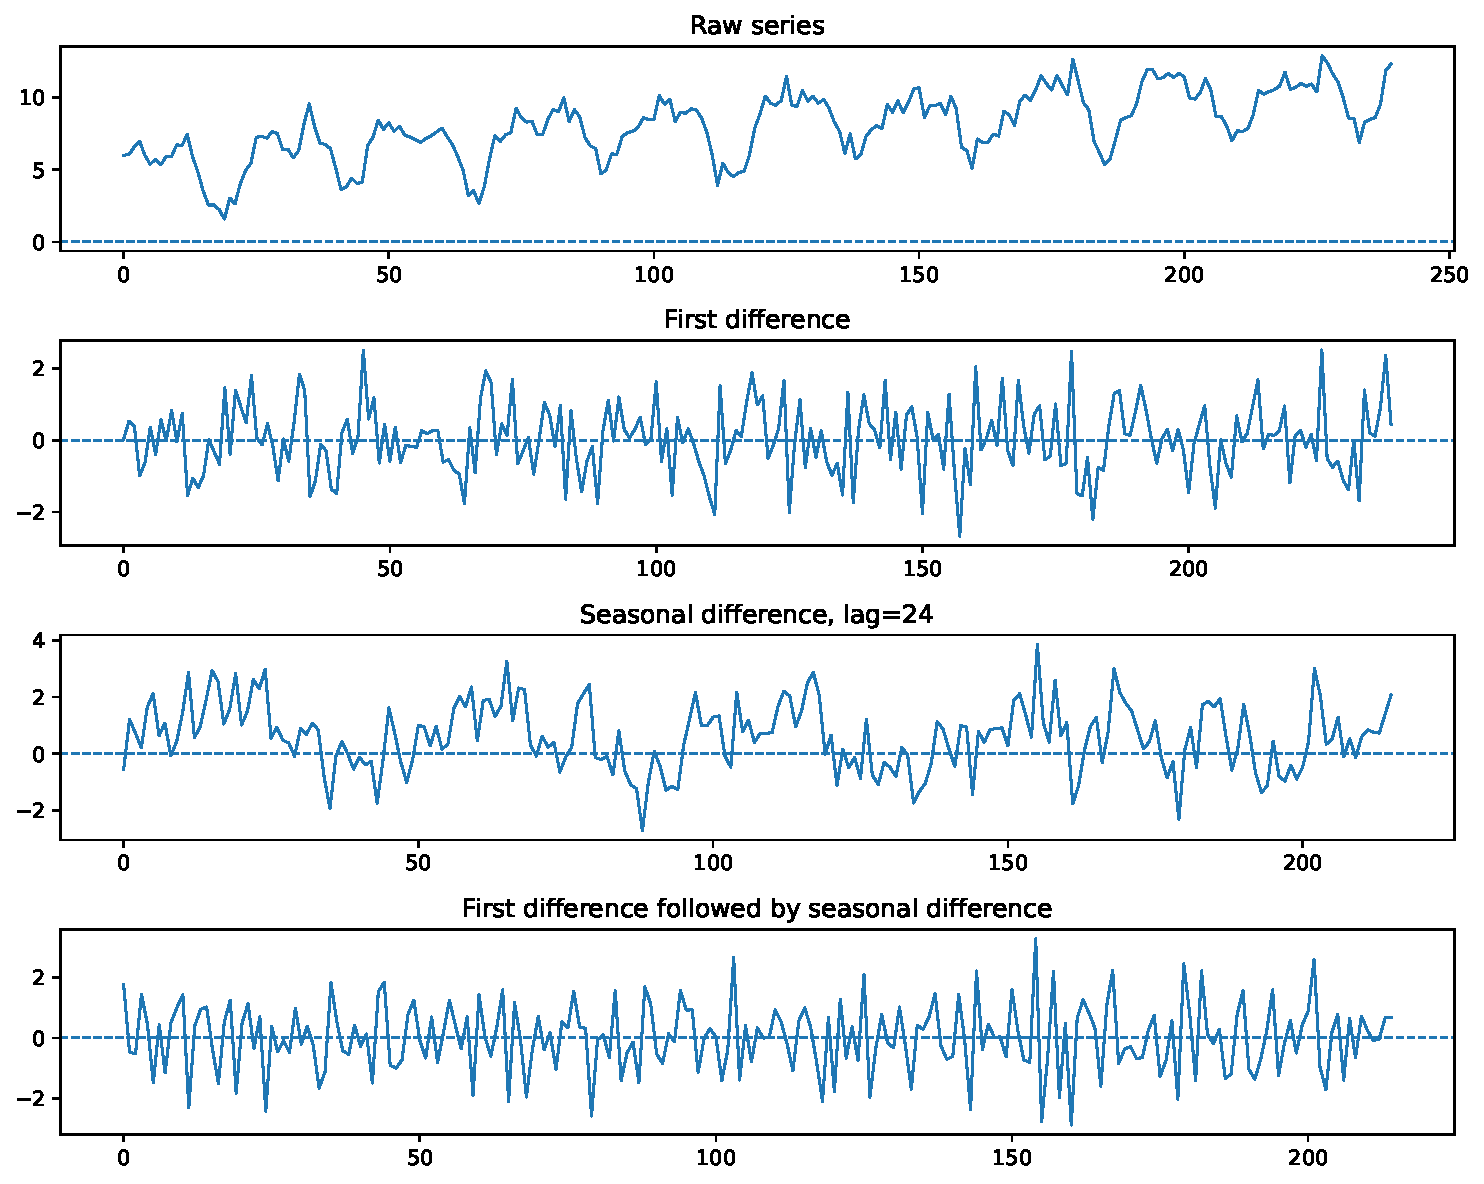
\includegraphics[keepaspectratio]{chapters/chapter-02-exploratory-data-analysis_files/figure-pdf/ch02-differencing-plot-output-1.pdf}}

\protect\phantomsection\label{ch02-differencing-acfs}
\begin{Shaded}
\begin{Highlighting}[]
\NormalTok{plot\_acf\_stems(first\_diff, max\_lag}\OperatorTok{=}\DecValTok{60}\NormalTok{, title}\OperatorTok{=}\StringTok{"ACF of first difference"}\NormalTok{)}
\NormalTok{plot\_acf\_stems(seasonal\_diff, max\_lag}\OperatorTok{=}\DecValTok{60}\NormalTok{, title}\OperatorTok{=}\StringTok{"ACF of seasonal difference"}\NormalTok{)}
\NormalTok{plot\_acf\_stems(combined\_diff, max\_lag}\OperatorTok{=}\DecValTok{60}\NormalTok{, title}\OperatorTok{=}\StringTok{"ACF of combined difference"}\NormalTok{)}
\end{Highlighting}
\end{Shaded}

\pandocbounded{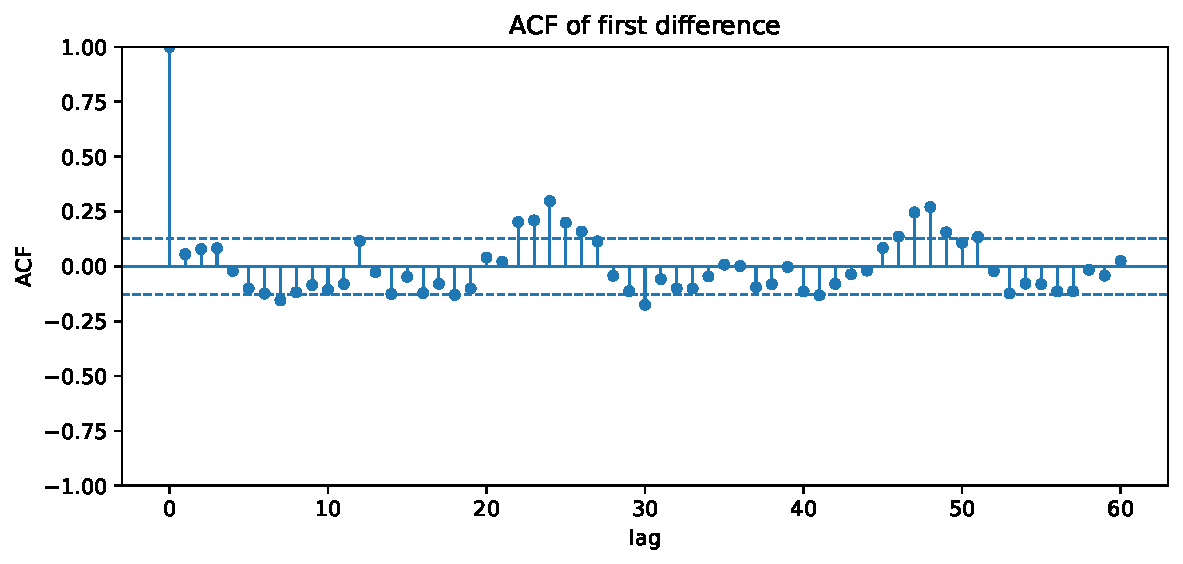
\includegraphics[keepaspectratio]{chapters/chapter-02-exploratory-data-analysis_files/figure-pdf/ch02-differencing-acfs-output-1.pdf}}

\pandocbounded{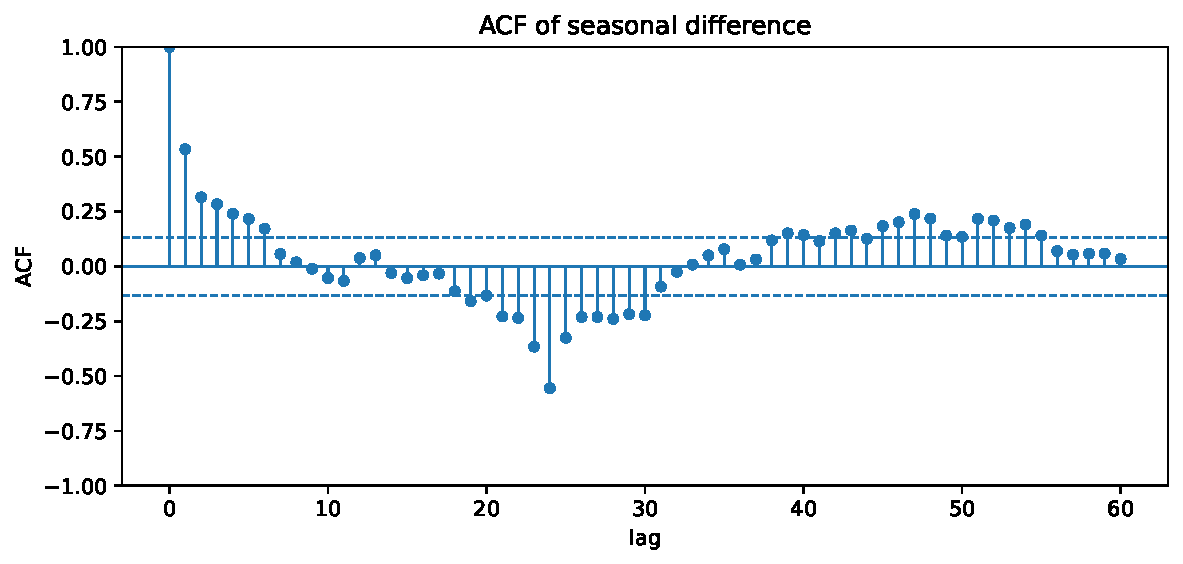
\includegraphics[keepaspectratio]{chapters/chapter-02-exploratory-data-analysis_files/figure-pdf/ch02-differencing-acfs-output-2.pdf}}

\pandocbounded{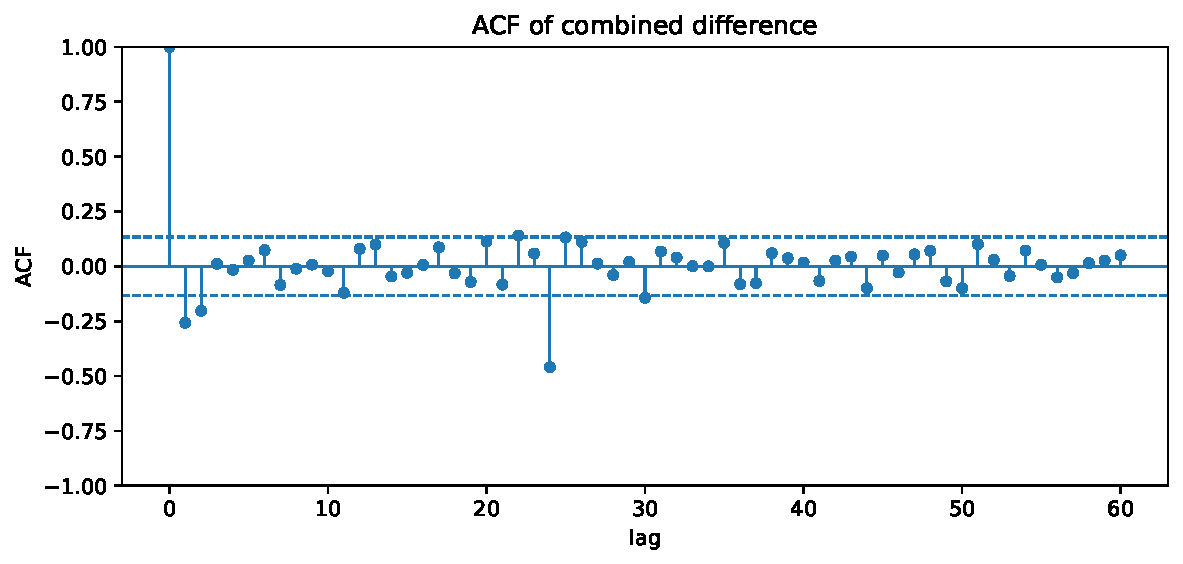
\includegraphics[keepaspectratio]{chapters/chapter-02-exploratory-data-analysis_files/figure-pdf/ch02-differencing-acfs-output-3.pdf}}

The point is not that one transformation is always best. The point is
that each transformation creates a different object. The EDA question
is: which transformed object has a dependence pattern that we can model
and validate?

\section{2.21 Python example: smoothing}\label{python-example-smoothing}

Smoothing can reveal slow trend but should not be confused with making a
series stationary.

\begin{Shaded}
\begin{Highlighting}[]
\NormalTok{s }\OperatorTok{=}\NormalTok{ pd.Series(x)}
\NormalTok{ma\_12 }\OperatorTok{=}\NormalTok{ s.rolling(window}\OperatorTok{=}\DecValTok{12}\NormalTok{, min\_periods}\OperatorTok{=}\DecValTok{1}\NormalTok{).mean()}
\NormalTok{ma\_24 }\OperatorTok{=}\NormalTok{ s.rolling(window}\OperatorTok{=}\DecValTok{24}\NormalTok{, min\_periods}\OperatorTok{=}\DecValTok{1}\NormalTok{).mean()}
\NormalTok{ewma }\OperatorTok{=}\NormalTok{ s.ewm(alpha}\OperatorTok{=}\FloatTok{0.12}\NormalTok{, adjust}\OperatorTok{=}\VariableTok{False}\NormalTok{).mean()}

\NormalTok{plt.figure(figsize}\OperatorTok{=}\NormalTok{(}\DecValTok{10}\NormalTok{, }\DecValTok{4}\NormalTok{))}
\NormalTok{plt.plot(t, x, linewidth}\OperatorTok{=}\FloatTok{0.7}\NormalTok{, label}\OperatorTok{=}\StringTok{"observed"}\NormalTok{)}
\NormalTok{plt.plot(t, ma\_12, linewidth}\OperatorTok{=}\DecValTok{2}\NormalTok{, label}\OperatorTok{=}\StringTok{"moving average, m=12"}\NormalTok{)}
\NormalTok{plt.plot(t, ma\_24, linewidth}\OperatorTok{=}\DecValTok{2}\NormalTok{, label}\OperatorTok{=}\StringTok{"moving average, m=24"}\NormalTok{)}
\NormalTok{plt.plot(t, ewma, linewidth}\OperatorTok{=}\DecValTok{2}\NormalTok{, linestyle}\OperatorTok{=}\StringTok{"{-}{-}"}\NormalTok{, label}\OperatorTok{=}\StringTok{"exponential smoothing, alpha=0.12"}\NormalTok{)}
\NormalTok{plt.xlabel(}\StringTok{"time"}\NormalTok{)}
\NormalTok{plt.ylabel(}\StringTok{"value"}\NormalTok{)}
\NormalTok{plt.title(}\StringTok{"Smoothing for exploratory visualization"}\NormalTok{)}
\NormalTok{plt.legend()}
\NormalTok{plt.show()}
\end{Highlighting}
\end{Shaded}

\pandocbounded{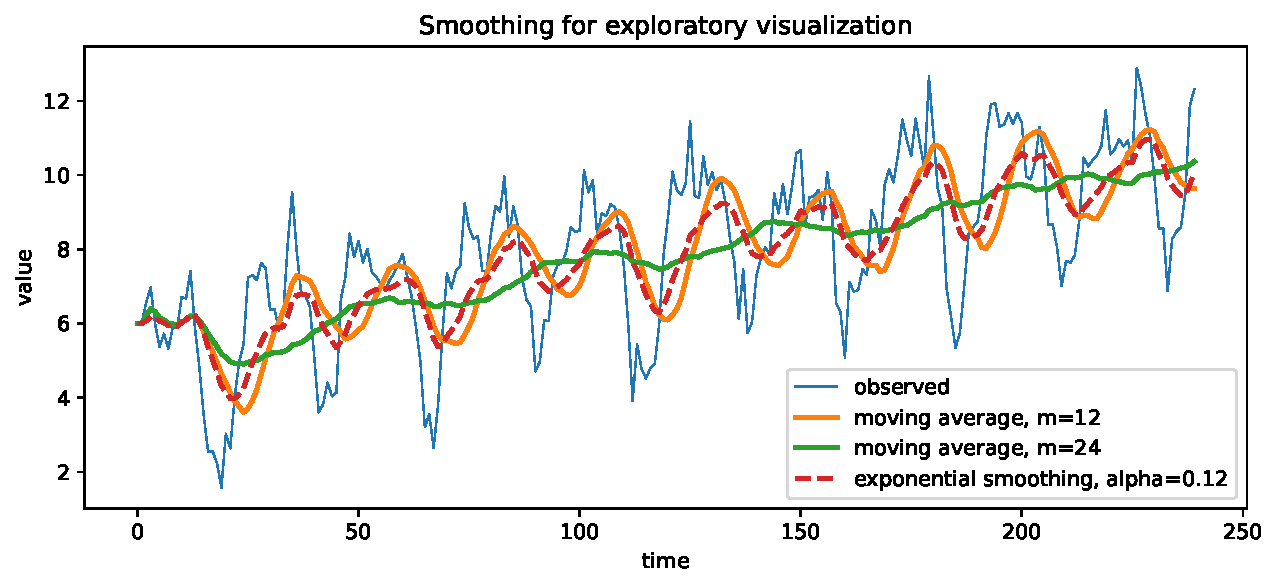
\includegraphics[keepaspectratio]{chapters/chapter-02-exploratory-data-analysis_files/figure-pdf/ch02-smoothing-output-1.pdf}}

\section{2.22 Python example: lag plots}\label{python-example-lag-plots}

Lag plots reveal dependence geometrically. For an AR(1)-like residual,
the lag-one plot often shows a linear pattern.

\begin{Shaded}
\begin{Highlighting}[]
\NormalTok{res }\OperatorTok{=}\NormalTok{ residual\_fourier}
\NormalTok{fig, axes }\OperatorTok{=}\NormalTok{ plt.subplots(}\DecValTok{2}\NormalTok{, }\DecValTok{2}\NormalTok{, figsize}\OperatorTok{=}\NormalTok{(}\DecValTok{8}\NormalTok{, }\DecValTok{8}\NormalTok{))}
\ControlFlowTok{for}\NormalTok{ ax, lag }\KeywordTok{in} \BuiltInTok{zip}\NormalTok{(axes.ravel(), [}\DecValTok{1}\NormalTok{, }\DecValTok{2}\NormalTok{, }\DecValTok{12}\NormalTok{, }\DecValTok{24}\NormalTok{]):}
\NormalTok{    ax.scatter(res[:}\OperatorTok{{-}}\NormalTok{lag], res[lag:], s}\OperatorTok{=}\DecValTok{16}\NormalTok{, alpha}\OperatorTok{=}\FloatTok{0.7}\NormalTok{)}
\NormalTok{    ax.set\_xlabel(}\SpecialStringTok{f"e[t{-}}\SpecialCharTok{\{}\NormalTok{lag}\SpecialCharTok{\}}\SpecialStringTok{]"}\NormalTok{)}
\NormalTok{    ax.set\_ylabel(}\StringTok{"e[t]"}\NormalTok{)}
\NormalTok{    ax.set\_title(}\SpecialStringTok{f"Lag plot, h=}\SpecialCharTok{\{}\NormalTok{lag}\SpecialCharTok{\}}\SpecialStringTok{"}\NormalTok{)}
\NormalTok{plt.tight\_layout()}
\NormalTok{plt.show()}
\end{Highlighting}
\end{Shaded}

\pandocbounded{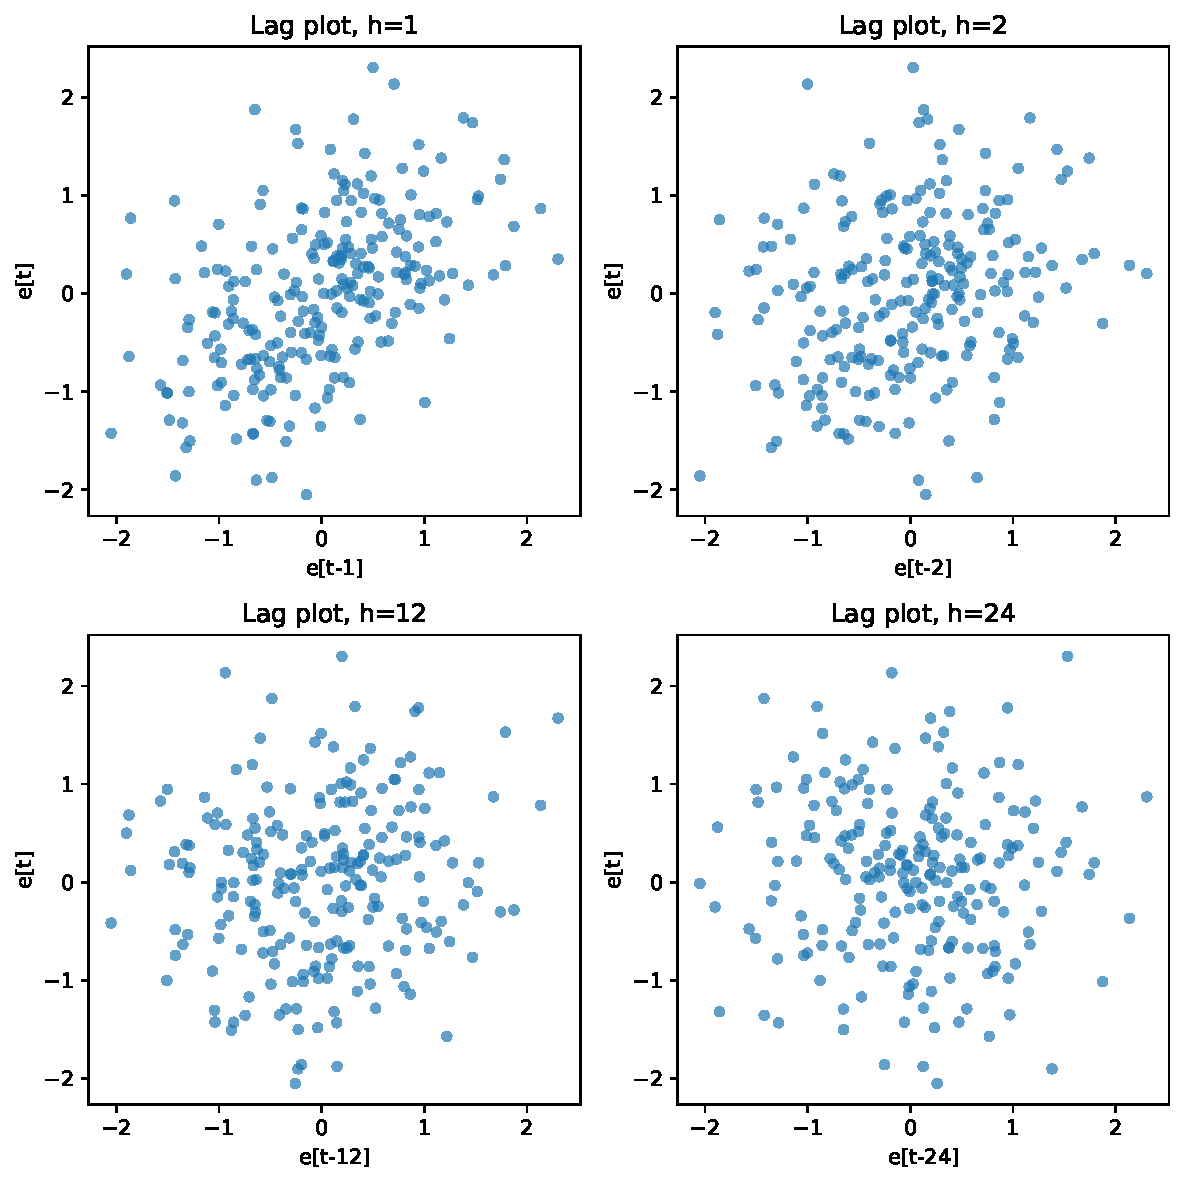
\includegraphics[keepaspectratio]{chapters/chapter-02-exploratory-data-analysis_files/figure-pdf/ch02-lag-plots-output-1.pdf}}

\section{2.23 A reproducible EDA checklist in
Python}\label{a-reproducible-eda-checklist-in-python}

The following function creates a compact EDA report for a univariate
sequence. It is intentionally simple. Later chapters will replace pieces
of this with more formal tests and models.

\begin{Shaded}
\begin{Highlighting}[]
\KeywordTok{def}\NormalTok{ quick\_eda\_report(values, period}\OperatorTok{=}\VariableTok{None}\NormalTok{, max\_lag}\OperatorTok{=}\DecValTok{40}\NormalTok{):}
\NormalTok{    values }\OperatorTok{=}\NormalTok{ pd.Series(np.asarray(values, dtype}\OperatorTok{=}\BuiltInTok{float}\NormalTok{)).dropna()}
\NormalTok{    report }\OperatorTok{=}\NormalTok{ \{}
        \StringTok{"n"}\NormalTok{: }\BuiltInTok{len}\NormalTok{(values),}
        \StringTok{"mean"}\NormalTok{: values.mean(),}
        \StringTok{"std"}\NormalTok{: values.std(),}
        \StringTok{"min"}\NormalTok{: values.}\BuiltInTok{min}\NormalTok{(),}
        \StringTok{"max"}\NormalTok{: values.}\BuiltInTok{max}\NormalTok{(),}
        \StringTok{"acf\_lag\_1"}\NormalTok{: sample\_acf(values, max\_lag}\OperatorTok{=}\DecValTok{1}\NormalTok{)[}\DecValTok{1}\NormalTok{] }\ControlFlowTok{if} \BuiltInTok{len}\NormalTok{(values) }\OperatorTok{\textgreater{}} \DecValTok{2} \ControlFlowTok{else}\NormalTok{ np.nan,}
\NormalTok{    \}}
    \ControlFlowTok{if}\NormalTok{ period }\KeywordTok{is} \KeywordTok{not} \VariableTok{None} \KeywordTok{and} \BuiltInTok{len}\NormalTok{(values) }\OperatorTok{\textgreater{}}\NormalTok{ period:}
\NormalTok{        report[}\SpecialStringTok{f"acf\_lag\_}\SpecialCharTok{\{}\NormalTok{period}\SpecialCharTok{\}}\SpecialStringTok{"}\NormalTok{] }\OperatorTok{=}\NormalTok{ sample\_acf(values, max\_lag}\OperatorTok{=}\NormalTok{period)[period]}
    \ControlFlowTok{return}\NormalTok{ pd.Series(report)}

\NormalTok{pd.DataFrame(\{}
    \StringTok{"raw"}\NormalTok{: quick\_eda\_report(x, period}\OperatorTok{=}\NormalTok{period),}
    \StringTok{"trend\_seasonal\_residual"}\NormalTok{: quick\_eda\_report(residual\_fourier, period}\OperatorTok{=}\NormalTok{period),}
    \StringTok{"first\_diff"}\NormalTok{: quick\_eda\_report(first\_diff, period}\OperatorTok{=}\NormalTok{period),}
    \StringTok{"seasonal\_diff"}\NormalTok{: quick\_eda\_report(seasonal\_diff, period}\OperatorTok{=}\NormalTok{period),}
\NormalTok{\})}
\end{Highlighting}
\end{Shaded}

\protect\phantomsection\label{ch02-eda-report-function}
{\def\LTcaptype{none} % do not increment counter
\begin{longtable}[]{@{}lllll@{}}
\toprule\noalign{}
& raw & trend\_seasonal\_residual & first\_diff & seasonal\_diff \\
\midrule\noalign{}
\endhead
\bottomrule\noalign{}
\endlastfoot
n & 240.000000 & 2.400000e+02 & 239.000000 & 216.000000 \\
mean & 7.988363 & 2.590520e-16 & 0.026387 & 0.603315 \\
std & 2.290297 & 8.144020e-01 & 0.968605 & 1.174616 \\
min & 1.575312 & -2.049972e+00 & -2.669879 & -2.720756 \\
max & 12.890898 & 2.302720e+00 & 2.513365 & 3.860035 \\
acf\_lag\_1 & 0.901865 & 4.829578e-01 & 0.055540 & 0.533595 \\
acf\_lag\_24 & 0.659006 & -2.874861e-02 & 0.297357 & -0.555331 \\
\end{longtable}
}

A report like this does not replace plots, but it helps make EDA
reproducible and comparable across transformations.

\section{2.24 Connection to machine learning
features}\label{connection-to-machine-learning-features}

Classical EDA naturally creates features for machine learning models.
Suppose we want to predict \(x_{t+1}\). Candidate features include:

\[
x_t,x_{t-1},\dots,x_{t-L+1},
\]

rolling summaries such as

\[
\frac{1}{m}\sum_{j=0}^{m-1}x_{t-j},
\]

calendar indicators, and Fourier features such as

\[
\cos\left(\frac{2\pi kt}{s}\right),\qquad
\sin\left(\frac{2\pi kt}{s}\right).
\]

A feature-based ML model might use

\[
\widehat x_{t+1}=f\left(x_t,x_{t-1},\dots,\text{rolling mean},\text{Fourier features},\text{calendar features}\right).
\]

This connects EDA to later chapters on feature-based ML, CNNs, RNNs, and
transformers. Deep models can learn features, but human-designed
exploratory features remain valuable baselines and diagnostic tools.

\section{2.25 AI-assisted study: use AI to generate hypotheses, not
conclusions}\label{ai-assisted-study-use-ai-to-generate-hypotheses-not-conclusions}

AI tools can accelerate EDA when used carefully. They are especially
useful for creating diagnostic checklists, identifying possible causes
of a pattern, and translating visual observations into candidate models.
They are dangerous when they choose a final model without seeing the
data, validation design, and residual diagnostics.

\section{AI-assisted EDA prompt}\label{ai-assisted-eda-prompt}

Use this prompt after you have created a time plot, rolling mean,
rolling variance, and ACF.

\begin{quote}
I am doing exploratory data analysis for a univariate time series. The
time plot shows {[}describe trend/seasonality/outliers{]}. The rolling
variance shows {[}describe scale{]}. The ACF shows {[}describe
decay/spikes{]}. Give me five plausible data-generating explanations.
For each explanation, give: (1) the mathematical form, (2) one
diagnostic plot to check, (3) one transformation or preprocessing step,
(4) one simple baseline forecast, and (5) one way this explanation could
be wrong. Do not select a final model yet.
\end{quote}

\section{AI code-checking prompt}\label{ai-code-checking-prompt}

After writing code, ask:

\begin{quote}
Check this time-series EDA code for leakage, misuse of random train-test
splitting, incorrect differencing alignment, missing inverse
transformation, and misleading interpretation of smoothed data. Explain
each issue in terms of the time index.
\end{quote}

\section{2.26 Mini case study: from raw data to modeling
plan}\label{mini-case-study-from-raw-data-to-modeling-plan}

Imagine a daily demand series with weekly seasonality and a slowly
increasing level. A good EDA summary might be:

\begin{enumerate}
\def\labelenumi{\arabic{enumi}.}
\tightlist
\item
  The raw time plot shows an upward trend and repeated weekly peaks.
\item
  Rolling variance is roughly stable after a log transform.
\item
  The ACF decays slowly in the raw series and has spikes at lags 7, 14,
  and 21.
\item
  First differencing reduces trend, but weekly spikes remain.
\item
  Seasonal differencing at lag 7 reduces the seasonal pattern.
\item
  Candidate baselines: naive, seasonal naive, and rolling mean.
\item
  Candidate models: SARIMA, Prophet-style additive model, and
  lag-feature gradient boosting.
\item
  Validation should use rolling-origin or blocked time splits, not
  random splitting.
\end{enumerate}

This is the level of reasoning expected before fitting a model.

\section{2.27 Mathematical summary}\label{mathematical-summary-1}

{\def\LTcaptype{none} % do not increment counter
\begin{longtable}[]{@{}
  >{\raggedright\arraybackslash}p{(\linewidth - 4\tabcolsep) * \real{0.3000}}
  >{\raggedleft\arraybackslash}p{(\linewidth - 4\tabcolsep) * \real{0.4000}}
  >{\raggedright\arraybackslash}p{(\linewidth - 4\tabcolsep) * \real{0.3000}}@{}}
\toprule\noalign{}
\begin{minipage}[b]{\linewidth}\raggedright
Concept
\end{minipage} & \begin{minipage}[b]{\linewidth}\raggedleft
Formula
\end{minipage} & \begin{minipage}[b]{\linewidth}\raggedright
Purpose
\end{minipage} \\
\midrule\noalign{}
\endhead
\bottomrule\noalign{}
\endlastfoot
Additive decomposition & \(X_t=T_t+S_t+Y_t\) & Separate trend,
seasonality, residual dependence \\
Regression trend & \(x=Z\beta+e\) & Estimate deterministic mean
structure \\
OLS estimate & \(\widehat\beta=(Z^TZ)^{-1}Z^Tx\) & Fit trend or seasonal
features \\
Fourier seasonality & \(\sum_k a_k\cos(2\pi kt/s)+b_k\sin(2\pi kt/s)\) &
Model periodic mean components \\
First difference & \(\nabla x_t=x_t-x_{t-1}\) & Remove linear stochastic
or deterministic drift \\
Seasonal difference & \(\nabla_s x_t=x_t-x_{t-s}\) & Remove seasonal
level pattern \\
Moving average smoother &
\(\widetilde x_t=m^{-1}\sum_{j=0}^{m-1}x_{t-j}\) & Reveal slow
structure \\
Exponential smoother & \(\ell_t=\alpha x_t+(1-\alpha)\ell_{t-1}\) &
Smooth with decaying memory \\
Sample ACF & \(\widehat\rho(h)=\widehat\gamma(h)/\widehat\gamma(0)\) &
Diagnose serial dependence \\
\end{longtable}
}

\section{2.28 Common mistakes}\label{common-mistakes-1}

\begin{enumerate}
\def\labelenumi{\arabic{enumi}.}
\tightlist
\item
  \textbf{Treating smoothing as modeling.} A smoother helps
  visualization; it is not automatically a forecast model.
\item
  \textbf{Removing trend and ignoring residual dependence.} Detrended
  residuals can still be autocorrelated.
\item
  \textbf{Over-differencing.} Too much differencing can introduce
  artificial negative autocorrelation.
\item
  \textbf{Ignoring scale.} If variability grows with the level, a log or
  Box-Cox transform may be necessary.
\item
  \textbf{Confusing deterministic seasonality with seasonal dependence.}
  Fourier regression and seasonal AR terms solve different problems.
\item
  \textbf{Using future information in feature construction.} Centered
  rolling averages can leak future values if used for forecasting
  features.
\item
  \textbf{Letting AI choose a final model from a verbal description
  only.} AI can suggest hypotheses, but diagnostics and validation
  decide.
\end{enumerate}

\section{2.29 Exercises}\label{exercises-1}

\subsection{Conceptual exercises}\label{conceptual-exercises-1}

\begin{enumerate}
\def\labelenumi{\arabic{enumi}.}
\tightlist
\item
  Explain the difference between detrending and differencing using the
  model \(x_t=\mu_t+y_t\).
\item
  Suppose \(x_t=\beta_0+\beta_1t+y_t\). Compute \(\nabla x_t\) and
  identify what happened to the intercept and slope.
\item
  Suppose \(x_t\) has monthly seasonality. Write the seasonal difference
  operator.
\item
  Explain why a log transform can stabilize variance for multiplicative
  models.
\item
  Give one example where smoothing is helpful and one example where
  smoothing could be misleading.
\end{enumerate}

\subsection{Mathematical exercises}\label{mathematical-exercises}

\begin{enumerate}
\def\labelenumi{\arabic{enumi}.}
\tightlist
\item
  Prove that the second difference of a linear function is zero.
\item
  Show that if \(y_t\) is white noise with variance \(\sigma^2\), then
  \(z_t=y_t-y_{t-1}\) has \(\operatorname{Cov}(z_t,z_{t-1})=-\sigma^2\).
\item
  Derive the least-squares normal equation \(Z^TZ\widehat\beta=Z^Tx\).
\item
  Show that \(A\cos(2\pi\omega t+\phi)\) can be written as
  \(a\cos(2\pi\omega t)+b\sin(2\pi\omega t)\).
\item
  For a moving-average smoother with weights \(a_0,\dots,a_{m-1}\), what
  condition on the weights preserves a constant mean?
\end{enumerate}

\subsection{Computational exercises}\label{computational-exercises-1}

\begin{enumerate}
\def\labelenumi{\arabic{enumi}.}
\tightlist
\item
  Simulate a series with a quadratic trend and white-noise errors.
  Compare first and second differencing.
\item
  Simulate a multiplicative seasonal series. Apply a log transform and
  compare rolling variance before and after transformation.
\item
  Write your own function for seasonal differencing and test it on a
  period-12 series.
\item
  Fit a regression model with trend and Fourier seasonal features. Plot
  residuals and their ACF.
\item
  Create lag plots for lags 1, 2, 7, and 14 for a daily seasonal series.
  Interpret the visual patterns.
\item
  Build a compact EDA report for a real data set and write a modeling
  plan.
\end{enumerate}

\subsection{AI-assisted exercise}\label{ai-assisted-exercise-1}

Use an AI assistant to critique your EDA report. Your final submission
should include:

\begin{enumerate}
\def\labelenumi{\arabic{enumi}.}
\tightlist
\item
  your original EDA summary;
\item
  the AI's proposed concerns;
\item
  which concerns you verified with code;
\item
  which concerns you rejected and why;
\item
  your revised modeling plan.
\end{enumerate}

\section{2.30 Chapter checklist}\label{chapter-checklist-1}

Before moving to Chapter 3, make sure you can do the following without
notes:

\begin{itemize}
\tightlist
\item
  write the additive decomposition \(X_t=T_t+S_t+Y_t\);
\item
  explain when a log transform is useful;
\item
  compute and interpret first and seasonal differences;
\item
  fit a trend using least squares;
\item
  fit deterministic seasonality using sine and cosine features;
\item
  compute a sample ACF from scratch;
\item
  explain why over-differencing can introduce dependence;
\item
  create a time-series EDA report that leads to a modeling plan;
\item
  use an AI assistant to generate hypotheses while preserving
  mathematical verification.
\end{itemize}

\section{Further reading}\label{further-reading-1}

Classical exploratory analysis, detrending, differencing, smoothing, and
autocorrelation diagnostics are developed in {[}1{]} and {[}2{]}.
Forecasting workflows and practical decomposition ideas are expanded in
{[}3{]}. The Fourier-feature approach also connects to automated
additive forecasting models such as {[}4{]}.

\part{Part II. Stationarity and Linear Time-Domain Models}

\chapter{Stationarity, Autocovariance, and
Autocorrelation}\label{stationarity-autocovariance-and-autocorrelation}

\textbf{Part II. Stationarity and Linear Time-Domain Models}\\
\textbf{Chapter goal:} learn the mathematical language used to describe
stable dependence in a time series: stationarity, mean functions,
autocovariance, autocorrelation, sample ACF, and the first diagnostic
signatures of white noise, random walks, MA(1), and AR(1) processes.

\section{Learning objectives}\label{learning-objectives-2}

After studying this chapter, you should be able to:

\begin{enumerate}
\def\labelenumi{\arabic{enumi}.}
\tightlist
\item
  distinguish strict stationarity from weak stationarity;
\item
  define the mean function, autocovariance function, autocorrelation
  function, and sample ACF;
\item
  explain why stationarity makes dependence estimable from one observed
  path;
\item
  prove that white noise and MA(1) processes are weakly stationary;
\item
  prove that a random walk is not weakly stationary;
\item
  derive the autocovariance and ACF of an AR(1) process;
\item
  interpret ACF plots for white noise, random walks, AR(1), MA(1),
  trends, and changing variance;
\item
  use Python to simulate processes, compute sample ACFs, and diagnose
  stationarity;
\item
  use AI tools to critique stationarity assumptions without replacing
  mathematical checks.
\end{enumerate}

\section{3.1 Why stationarity matters}\label{why-stationarity-matters}

Time-series data are usually observed as one path

\[
x_1,x_2,\\dots,x_n
\]

from a stochastic process

\[
\{X_t:t\in \mathbb Z\}.
\]

For independent data, we often rely on repeated independent
observations. In time series, the observations are dependent, and often
we only have one historical path. To learn anything from that path, we
need some form of stability. \textbf{Stationarity} is the most important
stability assumption.

Informally, a stationary process has probabilistic behavior that does
not change when the time origin is shifted. A window of length 20 from
the beginning of the series should be governed by the same probabilistic
rules as a window of length 20 later in the series. The realized values
may differ, but the distributional rules are stable.

\begin{tcolorbox}[enhanced jigsaw, arc=.35mm, bottomrule=.15mm, bottomtitle=1mm, breakable, colback=white, colbacktitle=quarto-callout-note-color!10!white, colframe=quarto-callout-note-color-frame, coltitle=black, left=2mm, leftrule=.75mm, opacityback=0, opacitybacktitle=0.6, rightrule=.15mm, title=\textcolor{quarto-callout-note-color}{\faInfo}\hspace{0.5em}{Why this is not just a technical condition}, titlerule=0mm, toprule=.15mm, toptitle=1mm]

If dependence changes over time, then observations from the past may not
represent the future. A forecasting model trained on old data may be
solving the wrong problem. Stationarity is the assumption that makes the
past informative about the future in a controlled way.

\end{tcolorbox}

This chapter begins with two levels of stationarity:

\begin{itemize}
\tightlist
\item
  \textbf{strict stationarity}, which is a condition on all
  finite-dimensional distributions;
\item
  \textbf{weak stationarity}, which is a condition only on first and
  second moments.
\end{itemize}

Most of classical ARMA theory uses weak stationarity. For Gaussian
processes, weak stationarity and strict stationarity are closely
connected because means and covariances determine all finite-dimensional
Gaussian distributions.

\section{3.2 Strict stationarity}\label{strict-stationarity}

Let \(\{X_t:t\in\mathbb Z\}\) be a stochastic process. It is
\textbf{strictly stationary} if, for every integer \(k\ge 1\), every set
of time points \(t_1,\dots,t_k\), every shift \(h\), and every vector
\((x_1,\dots,x_k)\),

\[
P(X_{t_1}\le x_1,\dots,X_{t_k}\le x_k)
=
P(X_{t_1+h}\le x_1,\dots,X_{t_k+h}\le x_k).
\]

Equivalently,

\[
(X_{t_1},\dots,X_{t_k})
\overset{d}{=}
(X_{t_1+h},\dots,X_{t_k+h})
\]

for all choices of \(k\), \(t_1,\dots,t_k\), and \(h\).

The phrase \(\overset{d}{=}\) means equality in distribution. Strict
stationarity says that the joint distribution of any finite window
depends only on the relative arrangement of the time points, not on
their absolute position on the calendar.

\subsection{Example: iid sequence}\label{example-iid-sequence}

If \(X_t\) are independent and identically distributed, then the process
is strictly stationary. Shifting time changes the labels but not the
joint distribution.

\subsection{Example: deterministic trend plus
noise}\label{example-deterministic-trend-plus-noise}

Let

\[
X_t=\beta_0+\beta_1t+W_t,
\]

where \(W_t\) are iid \(N(0,\sigma^2)\) and \(\beta_1\ne0\). Then
\(X_t\) is not strictly stationary because

\[
E[X_t]=\beta_0+\beta_1t
\]

changes with \(t\). A window later in time is centered at a different
level.

\subsection{Example: changing variance}\label{example-changing-variance}

Let

\[
X_t=\sigma_t W_t,
\]

where \(W_t\) are iid \(N(0,1)\) and \(\sigma_t\) changes with \(t\).
Then

\[
\operatorname{Var}(X_t)=\sigma_t^2
\]

changes with \(t\), so the process is not stationary.

\begin{tcolorbox}[enhanced jigsaw, arc=.35mm, bottomrule=.15mm, bottomtitle=1mm, breakable, colback=white, colbacktitle=quarto-callout-tip-color!10!white, colframe=quarto-callout-tip-color-frame, coltitle=black, left=2mm, leftrule=.75mm, opacityback=0, opacitybacktitle=0.6, rightrule=.15mm, title=\textcolor{quarto-callout-tip-color}{\faLightbulb}\hspace{0.5em}{Visual clue}, titlerule=0mm, toprule=.15mm, toptitle=1mm]

A trend violates stable mean. A changing spread violates stable
variance. A changing dependence pattern violates stable covariance. Any
one of these is enough to make a process nonstationary.

\end{tcolorbox}

\section{3.3 Mean function, autocovariance, and
autocorrelation}\label{mean-function-autocovariance-and-autocorrelation}

Assume \(E[X_t^2]<\infty\) for all \(t\). The \textbf{mean function} is

\[
\mu_t=E[X_t].
\]

The \textbf{autocovariance function} is

\[
\gamma_X(s,t)=\operatorname{Cov}(X_s,X_t)
=E[(X_s-\mu_s)(X_t-\mu_t)].
\]

The \textbf{autocorrelation function} is

\[
\rho_X(s,t)=\operatorname{Corr}(X_s,X_t)
=
\frac{\gamma_X(s,t)}{\sqrt{\gamma_X(s,s)\gamma_X(t,t)}}
\]

when the variances are positive.

Autocovariance measures linear dependence between two time-indexed
random variables. If \(X_t\) and \(X_{t+h}\) tend to move together,
\(\gamma_X(t+h,t)\) is positive. If they tend to move in opposite
directions, it is negative. If there is no linear dependence, it is
zero.

\begin{tcolorbox}[enhanced jigsaw, arc=.35mm, bottomrule=.15mm, bottomtitle=1mm, breakable, colback=white, colbacktitle=quarto-callout-important-color!10!white, colframe=quarto-callout-important-color-frame, coltitle=black, left=2mm, leftrule=.75mm, opacityback=0, opacitybacktitle=0.6, rightrule=.15mm, title=\textcolor{quarto-callout-important-color}{\faExclamation}\hspace{0.5em}{Covariance is not independence}, titlerule=0mm, toprule=.15mm, toptitle=1mm]

Zero covariance does not imply independence in general. It means no
linear dependence. If the process is jointly Gaussian, then zero
covariance does imply independence. This distinction matters when we
move from classical Gaussian models to nonlinear sequence models.

\end{tcolorbox}

\section{3.4 Weak stationarity}\label{weak-stationarity}

A process \(\{X_t\}\) with finite second moments is \textbf{weakly
stationary}, or \textbf{second-order stationary}, if:

\begin{enumerate}
\def\labelenumi{\arabic{enumi}.}
\tightlist
\item
  the mean is constant:
\end{enumerate}

\[
\mu_t=\mu
\]

for all \(t\);

\begin{enumerate}
\def\labelenumi{\arabic{enumi}.}
\setcounter{enumi}{1}
\tightlist
\item
  the autocovariance depends only on the lag \(h\), not on the absolute
  time \(t\):
\end{enumerate}

\[
\gamma_X(t+h,t)=\gamma_X(h).
\]

Thus, under weak stationarity, we write

\[
\gamma(h)=\operatorname{Cov}(X_{t+h},X_t),
\]

and

\[
\rho(h)=\frac{\gamma(h)}{\gamma(0)}.
\]

Because covariance is symmetric,

\[
\gamma(-h)=\gamma(h),
\]

and therefore

\[
\rho(-h)=\rho(h).
\]

The number \(\gamma(0)\) is the variance:

\[
\gamma(0)=\operatorname{Var}(X_t).
\]

The normalized quantity \(\rho(h)\) satisfies

\[
-1\le \rho(h)\le 1,
\]

and \(\rho(0)=1\).

\begin{tcolorbox}[enhanced jigsaw, arc=.35mm, bottomrule=.15mm, bottomtitle=1mm, breakable, colback=white, colbacktitle=quarto-callout-note-color!10!white, colframe=quarto-callout-note-color-frame, coltitle=black, left=2mm, leftrule=.75mm, opacityback=0, opacitybacktitle=0.6, rightrule=.15mm, title=\textcolor{quarto-callout-note-color}{\faInfo}\hspace{0.5em}{Strict versus weak stationarity}, titlerule=0mm, toprule=.15mm, toptitle=1mm]

Strict stationarity is about the full joint distribution. Weak
stationarity is only about \(E[X_t]\), \(\operatorname{Var}(X_t)\), and
\(\operatorname{Cov}(X_{t+h},X_t)\). Weak stationarity is easier to
check and is sufficient for much of ARMA theory.

\end{tcolorbox}

\section{3.5 Estimating dependence from one
path}\label{estimating-dependence-from-one-path}

Why does weak stationarity help? Suppose we want to estimate the
lag-\(h\) covariance. Without stationarity, the covariance

\[
\operatorname{Cov}(X_{t+h},X_t)
\]

could be different for every \(t\). We would have only one observation
of each pair, which is not enough.

With weak stationarity, all pairs

\[
(X_{1+h},X_1),(X_{2+h},X_2),\dots,(X_n,X_{n-h})
\]

share the same lag-\(h\) covariance structure. We can average
information across time. This is the key reason that stationarity is
useful.

For observed data \(x_1,\dots,x_n\), define the sample mean

\[
\bar x=\frac{1}{n}\sum_{t=1}^n x_t.
\]

A common sample autocovariance estimator is

\[
\widehat\gamma(h)
=\frac{1}{n}\sum_{t=1}^{n-h}(x_{t+h}-\bar x)(x_t-\bar x),
\qquad h=0,1,\dots,n-1.
\]

Then the sample autocorrelation is

\[
\widehat\rho(h)=\frac{\widehat\gamma(h)}{\widehat\gamma(0)}.
\]

Some software uses \(1/(n-h)\) instead of \(1/n\) in
\(\widehat\gamma(h)\). Both conventions appear in practice. The ACF plot
is usually more important than the small finite-sample difference
between these normalizations.

\section{3.6 White noise}\label{white-noise-1}

A process \(\{W_t\}\) is \textbf{white noise} with mean \(0\) and
variance \(\sigma^2\) if

\[
E[W_t]=0,
\]

\[
\operatorname{Var}(W_t)=\sigma^2,
\]

and

\[
\operatorname{Cov}(W_s,W_t)=0
\quad \text{for } s\ne t.
\]

We write

\[
W_t\sim WN(0,\sigma^2).
\]

White noise is weakly stationary because the mean is constant and the
covariance depends only on whether the lag is zero:

\[
\gamma(h)=
\begin{cases}
\sigma^2, & h=0,\\
0, & h\ne0.
\end{cases}
\]

Therefore,

\[
\rho(h)=
\begin{cases}
1, & h=0,\\
0, & h\ne0.
\end{cases}
\]

If the \(W_t\) are also independent and identically distributed, then
the process is \textbf{iid white noise}. If the \(W_t\) are iid
Gaussian, then it is \textbf{Gaussian white noise}.

\begin{tcolorbox}[enhanced jigsaw, arc=.35mm, bottomrule=.15mm, bottomtitle=1mm, breakable, colback=white, colbacktitle=quarto-callout-warning-color!10!white, colframe=quarto-callout-warning-color-frame, coltitle=black, left=2mm, leftrule=.75mm, opacityback=0, opacitybacktitle=0.6, rightrule=.15mm, title=\textcolor{quarto-callout-warning-color}{\faExclamationTriangle}\hspace{0.5em}{White noise is not necessarily independent noise}, titlerule=0mm, toprule=.15mm, toptitle=1mm]

The phrase white noise means uncorrelated over time with constant
variance. It does not automatically mean independent unless independence
is explicitly assumed or follows from a distributional assumption such
as joint Gaussianity.

\end{tcolorbox}

\subsection{Approximate ACF bands for white
noise}\label{approximate-acf-bands-for-white-noise}

For a long sample from white noise, the sample autocorrelations satisfy
approximately

\[
\widehat\rho(h)\approx N\left(0,\frac{1}{n}\right)
\]

for fixed \(h\ge1\). Thus, a common visual reference band is

\[
\pm \frac{1.96}{\sqrt n}.
\]

If many sample autocorrelations fall outside these bands, the
white-noise assumption is questionable. But some spikes may occur by
chance, especially when many lags are inspected.

\section{3.7 Random walks are not
stationary}\label{random-walks-are-not-stationary}

Let \(\{W_t\}\) be iid white noise with mean \(0\) and variance
\(\sigma^2\). Define the random walk

\[
S_t=\sum_{i=1}^t W_i.
\]

Equivalently,

\[
S_t=S_{t-1}+W_t.
\]

The mean is

\[
E[S_t]=\sum_{i=1}^t E[W_i]=0.
\]

But the variance is

\[
\operatorname{Var}(S_t)
=\operatorname{Var}\left(\sum_{i=1}^t W_i\right)
=t\sigma^2.
\]

The variance depends on \(t\), so \(\{S_t\}\) is not weakly stationary.

For \(h\ge0\),

\[
S_{t+h}=S_t+W_{t+1}+\cdots+W_{t+h}.
\]

Therefore,

\[
\operatorname{Cov}(S_{t+h},S_t)
=\operatorname{Cov}(S_t,S_t)=t\sigma^2.
\]

This also depends on \(t\). A random walk often looks persistent, but
that persistence comes from nonstationary accumulation rather than a
stable stationary correlation structure.

\subsection{Differencing the random
walk}\label{differencing-the-random-walk}

The first difference is

\[
\nabla S_t=S_t-S_{t-1}=W_t.
\]

Thus the random walk itself is nonstationary, but its first difference
is white noise. This is the simplest example behind ARIMA models.

\section{3.8 Moving-average example:
MA(1)}\label{moving-average-example-ma1}

Let \(\{W_t\}\sim WN(0,\sigma^2)\) and define

\[
X_t=W_t+\theta W_{t-1}.
\]

This is an MA(1) process. Its mean is

\[
E[X_t]=E[W_t]+\theta E[W_{t-1}]=0.
\]

Its variance is

\[
\gamma(0)=\operatorname{Var}(X_t)
=\operatorname{Var}(W_t+\theta W_{t-1})
=\sigma^2(1+\theta^2).
\]

For lag \(1\),

\[
\gamma(1)=\operatorname{Cov}(X_t,X_{t-1}).
\]

Since

\[
X_t=W_t+\theta W_{t-1},
\]

and

\[
X_{t-1}=W_{t-1}+\theta W_{t-2},
\]

only the shared term \(W_{t-1}\) contributes to the covariance. Hence,

\[
\gamma(1)=\theta\sigma^2.
\]

For \(|h|>1\), there is no overlapping white-noise term, so

\[
\gamma(h)=0.
\]

Therefore,

\[
\rho(h)=
\begin{cases}
1, & h=0,\\[4pt]
\dfrac{\theta}{1+\theta^2}, & |h|=1,\\[8pt]
0, & |h|>1.
\end{cases}
\]

This is the first example of a \textbf{cutoff ACF}: an MA(1) process has
nonzero autocorrelation only at lag \(1\).

\begin{tcolorbox}[enhanced jigsaw, arc=.35mm, bottomrule=.15mm, bottomtitle=1mm, breakable, colback=white, colbacktitle=quarto-callout-tip-color!10!white, colframe=quarto-callout-tip-color-frame, coltitle=black, left=2mm, leftrule=.75mm, opacityback=0, opacitybacktitle=0.6, rightrule=.15mm, title=\textcolor{quarto-callout-tip-color}{\faLightbulb}\hspace{0.5em}{Diagnostic signature of MA(q)}, titlerule=0mm, toprule=.15mm, toptitle=1mm]

An MA(\(q\)) process has theoretical ACF equal to zero for lags greater
than \(q\). In finite samples, the sample ACF will not be exactly zero,
but it should become statistically insignificant after lag \(q\).

\end{tcolorbox}

\section{3.9 Autoregressive example:
AR(1)}\label{autoregressive-example-ar1}

Let

\[
X_t=\phi X_{t-1}+W_t,
\]

where \(\{W_t\}\sim WN(0,\sigma^2)\). This is an AR(1) process.

If \(|\phi|<1\), the process has a causal stationary representation

\[
X_t=\sum_{j=0}^{\infty}\phi^j W_{t-j}.
\]

This representation shows that \(X_t\) is a weighted sum of current and
past shocks. The weights decay geometrically when \(|\phi|<1\).

Assuming stationarity and mean zero,

\[
E[X_t]=\phi E[X_{t-1}]+E[W_t]=\phi E[X_t].
\]

If \(\phi\ne1\), this gives

\[
E[X_t]=0.
\]

The variance satisfies

\[
\operatorname{Var}(X_t)
=\operatorname{Var}(\phi X_{t-1}+W_t)
=\phi^2\operatorname{Var}(X_{t-1})+\sigma^2.
\]

Stationarity gives
\(\operatorname{Var}(X_t)=\operatorname{Var}(X_{t-1})=\gamma(0)\), so

\[
\gamma(0)=\phi^2\gamma(0)+\sigma^2.
\]

Thus,

\[
\gamma(0)=\frac{\sigma^2}{1-\phi^2},
\qquad |\phi|<1.
\]

For \(h\ge1\),

\[
\gamma(h)=\operatorname{Cov}(X_{t+h},X_t).
\]

Using

\[
X_{t+h}=\phi X_{t+h-1}+W_{t+h},
\]

and the fact that \(W_{t+h}\) is uncorrelated with \(X_t\),

\[
\gamma(h)=\phi\gamma(h-1).
\]

By recursion,

\[
\gamma(h)=\phi^h\gamma(0),
\qquad h\ge0.
\]

By symmetry,

\[
\gamma(h)=\phi^{|h|}\gamma(0)
\]

when \(\phi^{|h|}\) is interpreted with sign according to \(\phi\). More
explicitly,

\[
\rho(h)=\phi^{|h|}.
\]

\subsection{\texorpdfstring{Interpretation of
\(\phi\)}{Interpretation of \textbackslash phi}}\label{interpretation-of-phi}

If \(0<\phi<1\), the ACF decays gradually and stays positive. The series
tends to be smooth and persistent.

If \(-1<\phi<0\), the ACF alternates signs:

\[
\rho(1)<0,\quad \rho(2)>0,\quad \rho(3)<0,\dots
\]

The series tends to zigzag.

If \(|\phi|\) is close to \(1\), dependence decays slowly. The process
may look nearly nonstationary in finite samples.

If \(|\phi|>1\), the recursion is explosive and does not have the usual
causal stationary solution.

\begin{tcolorbox}[enhanced jigsaw, arc=.35mm, bottomrule=.15mm, bottomtitle=1mm, breakable, colback=white, colbacktitle=quarto-callout-warning-color!10!white, colframe=quarto-callout-warning-color-frame, coltitle=black, left=2mm, leftrule=.75mm, opacityback=0, opacitybacktitle=0.6, rightrule=.15mm, title=\textcolor{quarto-callout-warning-color}{\faExclamationTriangle}\hspace{0.5em}{Slowly decaying ACF can mean different things}, titlerule=0mm, toprule=.15mm, toptitle=1mm]

A slowly decaying sample ACF can come from a stationary AR process with
\(\phi\) close to \(1\), but it can also indicate a trend, random walk,
seasonal structure, or regime change. Always combine the ACF with the
time plot and transformations.

\end{tcolorbox}

\section{3.10 Linear processes as a unifying
language}\label{linear-processes-as-a-unifying-language}

Many stationary linear time-series models can be written as

\[
X_t=\sum_{j=0}^{\infty}\psi_j W_{t-j},
\]

where \(\{W_t\}\) is white noise and the weights satisfy a summability
condition such as

\[
\sum_{j=0}^{\infty}|\psi_j|<\infty.
\]

This is called a \textbf{linear process}. The MA(1) model has

\[
\psi_0=1,\qquad \psi_1=\theta,\qquad \psi_j=0 \text{ for } j\ge2.
\]

The stationary AR(1) model has

\[
\psi_j=\phi^j,
\qquad j=0,1,2,\dots.
\]

For a linear process with mean zero,

\[
\gamma(h)=\sigma^2\sum_{j=0}^{\infty}\psi_j\psi_{j+|h|}.
\]

This formula explains why the ACF of a finite-order moving average cuts
off while the ACF of an autoregressive process usually decays gradually.

\section{3.11 Sample ACF as a diagnostic, not a
proof}\label{sample-acf-as-a-diagnostic-not-a-proof}

The sample ACF is one of the most useful diagnostic plots in time
series. But it should be interpreted carefully.

\subsection{White noise pattern}\label{white-noise-pattern}

For white noise, sample autocorrelations after lag zero should mostly
remain within approximate bands

\[
\pm\frac{1.96}{\sqrt n}.
\]

A few spikes can happen by chance.

\subsection{AR pattern}\label{ar-pattern}

For an AR(1) process, the ACF tends to decay geometrically. For
AR(\(p\)), the ACF usually decays rather than cutting off sharply.

\subsection{MA pattern}\label{ma-pattern}

For an MA(\(q\)) process, the ACF cuts off after lag \(q\) in theory.

\subsection{Trend or random-walk
pattern}\label{trend-or-random-walk-pattern}

For a trending or random-walk-like series, the sample ACF often decays
very slowly. This is a warning sign that the series may not be
stationary.

\subsection{Seasonal pattern}\label{seasonal-pattern}

For seasonal data, the ACF may show spikes at seasonal lags such as
\(7\), \(12\), \(24\), or \(365\), depending on the sampling frequency.

\begin{tcolorbox}[enhanced jigsaw, arc=.35mm, bottomrule=.15mm, bottomtitle=1mm, breakable, colback=white, colbacktitle=quarto-callout-important-color!10!white, colframe=quarto-callout-important-color-frame, coltitle=black, left=2mm, leftrule=.75mm, opacityback=0, opacitybacktitle=0.6, rightrule=.15mm, title=\textcolor{quarto-callout-important-color}{\faExclamation}\hspace{0.5em}{ACF diagnosis is comparative}, titlerule=0mm, toprule=.15mm, toptitle=1mm]

Do not ask only: ``What model does this ACF prove?'' Ask: ``Which models
are consistent with the time plot, ACF, PACF, residual diagnostics, and
validation performance?''

\end{tcolorbox}

\section{3.12 Interactive demonstration: stationarity and ACF
playground}\label{interactive-demonstration-stationarity-and-acf-playground}

The widget below simulates several processes and shows three views:

\begin{enumerate}
\def\labelenumi{\arabic{enumi}.}
\tightlist
\item
  the time plot;
\item
  rolling mean and rolling variance;
\item
  sample ACF with approximate white-noise bands.
\end{enumerate}

Use it to compare stationary and nonstationary behavior.

Process White noise Stationary AR(1) MA(1) Random walk Explosive AR(1)
Trend + noise Time-varying variance Sample size
\protect\phantomsection\label{ch03_n_val}{240} AR coefficient phi
\protect\phantomsection\label{ch03_phi_val}{0.70} MA coefficient theta
\protect\phantomsection\label{ch03_theta_val}{0.60}

\protect\phantomsection\label{ch03_ts_plot}

\protect\phantomsection\label{ch03_rolling_plot}

\protect\phantomsection\label{ch03_acf_plot}

Plotly.js is loaded once globally from assets/header.html; this chapter
uses the existing global Plotly object and does not load Plotly again.

\section{3.13 Python example: simulate and compare
processes}\label{python-example-simulate-and-compare-processes}

The following Python code simulates white noise, a random walk, an
MA(1), and an AR(1). The important point is not only to plot them, but
to compare their dependence structure.

\protect\phantomsection\label{ch03-python-simulate-processes}
\begin{Shaded}
\begin{Highlighting}[]
\ImportTok{import}\NormalTok{ numpy }\ImportTok{as}\NormalTok{ np}
\ImportTok{import}\NormalTok{ pandas }\ImportTok{as}\NormalTok{ pd}
\ImportTok{import}\NormalTok{ plotly.graph\_objects }\ImportTok{as}\NormalTok{ go}
\ImportTok{from}\NormalTok{ plotly.subplots }\ImportTok{import}\NormalTok{ make\_subplots}

\NormalTok{rng }\OperatorTok{=}\NormalTok{ np.random.default\_rng(}\DecValTok{7339}\NormalTok{)}
\NormalTok{n }\OperatorTok{=} \DecValTok{300}
\NormalTok{w }\OperatorTok{=}\NormalTok{ rng.normal(size}\OperatorTok{=}\NormalTok{n)}

\NormalTok{white\_noise }\OperatorTok{=}\NormalTok{ w}
\NormalTok{random\_walk }\OperatorTok{=}\NormalTok{ np.cumsum(w)}

\NormalTok{phi }\OperatorTok{=} \FloatTok{0.75}
\NormalTok{ar1 }\OperatorTok{=}\NormalTok{ np.zeros(n)}
\ControlFlowTok{for}\NormalTok{ t }\KeywordTok{in} \BuiltInTok{range}\NormalTok{(}\DecValTok{1}\NormalTok{, n):}
\NormalTok{    ar1[t] }\OperatorTok{=}\NormalTok{ phi }\OperatorTok{*}\NormalTok{ ar1[t}\OperatorTok{{-}}\DecValTok{1}\NormalTok{] }\OperatorTok{+}\NormalTok{ w[t]}

\NormalTok{theta }\OperatorTok{=} \FloatTok{0.70}
\NormalTok{ma1 }\OperatorTok{=}\NormalTok{ np.zeros(n)}
\ControlFlowTok{for}\NormalTok{ t }\KeywordTok{in} \BuiltInTok{range}\NormalTok{(n):}
\NormalTok{    ma1[t] }\OperatorTok{=}\NormalTok{ w[t] }\OperatorTok{+}\NormalTok{ theta }\OperatorTok{*}\NormalTok{ (w[t}\OperatorTok{{-}}\DecValTok{1}\NormalTok{] }\ControlFlowTok{if}\NormalTok{ t }\OperatorTok{\textgreater{}} \DecValTok{0} \ControlFlowTok{else} \FloatTok{0.0}\NormalTok{)}

\NormalTok{df }\OperatorTok{=}\NormalTok{ pd.DataFrame(\{}
    \StringTok{"time"}\NormalTok{: np.arange(}\DecValTok{1}\NormalTok{, n }\OperatorTok{+} \DecValTok{1}\NormalTok{),}
    \StringTok{"white\_noise"}\NormalTok{: white\_noise,}
    \StringTok{"random\_walk"}\NormalTok{: random\_walk,}
    \StringTok{"ar1\_phi\_075"}\NormalTok{: ar1,}
    \StringTok{"ma1\_theta\_070"}\NormalTok{: ma1,}
\NormalTok{\})}

\NormalTok{fig }\OperatorTok{=}\NormalTok{ make\_subplots(rows}\OperatorTok{=}\DecValTok{4}\NormalTok{, cols}\OperatorTok{=}\DecValTok{1}\NormalTok{, shared\_xaxes}\OperatorTok{=}\VariableTok{True}\NormalTok{, vertical\_spacing}\OperatorTok{=}\FloatTok{0.04}\NormalTok{)}
\NormalTok{series\_names }\OperatorTok{=}\NormalTok{ [}\StringTok{"white\_noise"}\NormalTok{, }\StringTok{"random\_walk"}\NormalTok{, }\StringTok{"ar1\_phi\_075"}\NormalTok{, }\StringTok{"ma1\_theta\_070"}\NormalTok{]}
\ControlFlowTok{for}\NormalTok{ i, name }\KeywordTok{in} \BuiltInTok{enumerate}\NormalTok{(series\_names, start}\OperatorTok{=}\DecValTok{1}\NormalTok{):}
\NormalTok{    fig.add\_trace(go.Scatter(x}\OperatorTok{=}\NormalTok{df[}\StringTok{"time"}\NormalTok{], y}\OperatorTok{=}\NormalTok{df[name], mode}\OperatorTok{=}\StringTok{"lines"}\NormalTok{, name}\OperatorTok{=}\NormalTok{name), row}\OperatorTok{=}\NormalTok{i, col}\OperatorTok{=}\DecValTok{1}\NormalTok{)}
\NormalTok{fig.update\_layout(height}\OperatorTok{=}\DecValTok{800}\NormalTok{, title}\OperatorTok{=}\StringTok{"Four simulated processes"}\NormalTok{)}
\NormalTok{fig.update\_xaxes(title\_text}\OperatorTok{=}\StringTok{"time"}\NormalTok{, row}\OperatorTok{=}\DecValTok{4}\NormalTok{, col}\OperatorTok{=}\DecValTok{1}\NormalTok{)}
\NormalTok{fig.show()}
\end{Highlighting}
\end{Shaded}

\protect\phantomsection\label{ch03-python-simulate-processes-1}
\begin{verbatim}
Unable to display output for mime type(s): text/html
\end{verbatim}

\protect\phantomsection\label{ch03-python-simulate-processes-2}
\begin{verbatim}
Unable to display output for mime type(s): text/html
\end{verbatim}

\section{3.14 Python example: compute the sample ACF from
scratch}\label{python-example-compute-the-sample-acf-from-scratch}

It is useful to implement the sample ACF manually before using a package
function.

\begin{Shaded}
\begin{Highlighting}[]
\ImportTok{import}\NormalTok{ numpy }\ImportTok{as}\NormalTok{ np}
\ImportTok{import}\NormalTok{ plotly.graph\_objects }\ImportTok{as}\NormalTok{ go}


\KeywordTok{def}\NormalTok{ sample\_acf(x, max\_lag):}
    \CommentTok{"""Biased sample ACF using denominator n, matching a common time{-}series convention."""}
\NormalTok{    x }\OperatorTok{=}\NormalTok{ np.asarray(x, dtype}\OperatorTok{=}\BuiltInTok{float}\NormalTok{)}
\NormalTok{    n }\OperatorTok{=} \BuiltInTok{len}\NormalTok{(x)}
\NormalTok{    x\_centered }\OperatorTok{=}\NormalTok{ x }\OperatorTok{{-}}\NormalTok{ x.mean()}
\NormalTok{    gamma0 }\OperatorTok{=}\NormalTok{ np.}\BuiltInTok{sum}\NormalTok{(x\_centered }\OperatorTok{*}\NormalTok{ x\_centered) }\OperatorTok{/}\NormalTok{ n}
\NormalTok{    values }\OperatorTok{=}\NormalTok{ []}
    \ControlFlowTok{for}\NormalTok{ h }\KeywordTok{in} \BuiltInTok{range}\NormalTok{(max\_lag }\OperatorTok{+} \DecValTok{1}\NormalTok{):}
\NormalTok{        gamma\_h }\OperatorTok{=}\NormalTok{ np.}\BuiltInTok{sum}\NormalTok{(x\_centered[h:] }\OperatorTok{*}\NormalTok{ x\_centered[: n }\OperatorTok{{-}}\NormalTok{ h]) }\OperatorTok{/}\NormalTok{ n}
\NormalTok{        values.append(gamma\_h }\OperatorTok{/}\NormalTok{ gamma0)}
    \ControlFlowTok{return}\NormalTok{ np.array(values)}

\NormalTok{max\_lag }\OperatorTok{=} \DecValTok{40}
\NormalTok{acf\_white }\OperatorTok{=}\NormalTok{ sample\_acf(white\_noise, max\_lag)}
\NormalTok{acf\_rw }\OperatorTok{=}\NormalTok{ sample\_acf(random\_walk, max\_lag)}
\NormalTok{acf\_ar1 }\OperatorTok{=}\NormalTok{ sample\_acf(ar1, max\_lag)}
\NormalTok{acf\_ma1 }\OperatorTok{=}\NormalTok{ sample\_acf(ma1, max\_lag)}

\NormalTok{lags }\OperatorTok{=}\NormalTok{ np.arange(max\_lag }\OperatorTok{+} \DecValTok{1}\NormalTok{)}
\NormalTok{ci }\OperatorTok{=} \FloatTok{1.96} \OperatorTok{/}\NormalTok{ np.sqrt(n)}

\NormalTok{fig }\OperatorTok{=}\NormalTok{ go.Figure()}
\ControlFlowTok{for}\NormalTok{ acf\_values, name }\KeywordTok{in}\NormalTok{ [}
\NormalTok{    (acf\_white, }\StringTok{"white noise"}\NormalTok{),}
\NormalTok{    (acf\_rw, }\StringTok{"random walk"}\NormalTok{),}
\NormalTok{    (acf\_ar1, }\StringTok{"AR(1), phi=0.75"}\NormalTok{),}
\NormalTok{    (acf\_ma1, }\StringTok{"MA(1), theta=0.70"}\NormalTok{),}
\NormalTok{]:}
\NormalTok{    fig.add\_trace(go.Scatter(x}\OperatorTok{=}\NormalTok{lags, y}\OperatorTok{=}\NormalTok{acf\_values, mode}\OperatorTok{=}\StringTok{"lines+markers"}\NormalTok{, name}\OperatorTok{=}\NormalTok{name))}
\NormalTok{fig.add\_hline(y}\OperatorTok{=}\NormalTok{ci, line\_dash}\OperatorTok{=}\StringTok{"dash"}\NormalTok{)}
\NormalTok{fig.add\_hline(y}\OperatorTok{={-}}\NormalTok{ci, line\_dash}\OperatorTok{=}\StringTok{"dash"}\NormalTok{)}
\NormalTok{fig.update\_layout(}
\NormalTok{    title}\OperatorTok{=}\StringTok{"Sample ACF comparison"}\NormalTok{,}
\NormalTok{    xaxis\_title}\OperatorTok{=}\StringTok{"lag"}\NormalTok{,}
\NormalTok{    yaxis\_title}\OperatorTok{=}\StringTok{"sample ACF"}\NormalTok{,}
\NormalTok{    yaxis\_range}\OperatorTok{=}\NormalTok{[}\OperatorTok{{-}}\DecValTok{1}\NormalTok{, }\DecValTok{1}\NormalTok{],}
\NormalTok{    height}\OperatorTok{=}\DecValTok{500}\NormalTok{,}
\NormalTok{)}
\NormalTok{fig.show()}
\end{Highlighting}
\end{Shaded}

\protect\phantomsection\label{ch03-python-acf-function}
\begin{verbatim}
Unable to display output for mime type(s): text/html
\end{verbatim}

The random walk usually shows a very slowly decaying sample ACF. That is
not evidence for a stationary AR model by itself. It is often evidence
that the original series is nonstationary and should be transformed or
differenced before fitting a stationary model.

\section{3.15 Python example: theoretical
ACFs}\label{python-example-theoretical-acfs}

For white noise, MA(1), and AR(1), the theoretical ACFs are explicit:

\[
\rho_{WN}(h)=0 \quad h\ge1,
\]

\[
\rho_{MA(1)}(1)=\frac{\theta}{1+\theta^2},
\qquad
\rho_{MA(1)}(h)=0 \quad h>1,
\]

and

\[
\rho_{AR(1)}(h)=\phi^h,\qquad h\ge0.
\]

\begin{Shaded}
\begin{Highlighting}[]
\NormalTok{phi }\OperatorTok{=} \FloatTok{0.75}
\NormalTok{alpha }\OperatorTok{=} \FloatTok{0.70}
\NormalTok{lags }\OperatorTok{=}\NormalTok{ np.arange(}\DecValTok{0}\NormalTok{, }\DecValTok{31}\NormalTok{)}

\NormalTok{rho\_wn }\OperatorTok{=}\NormalTok{ np.where(lags }\OperatorTok{==} \DecValTok{0}\NormalTok{, }\FloatTok{1.0}\NormalTok{, }\FloatTok{0.0}\NormalTok{)}
\NormalTok{rho\_ar1 }\OperatorTok{=}\NormalTok{ phi }\OperatorTok{**}\NormalTok{ lags}
\NormalTok{rho\_ma1 }\OperatorTok{=}\NormalTok{ np.zeros\_like(lags, dtype}\OperatorTok{=}\BuiltInTok{float}\NormalTok{)}
\NormalTok{rho\_ma1[}\DecValTok{0}\NormalTok{] }\OperatorTok{=} \FloatTok{1.0}
\NormalTok{rho\_ma1[}\DecValTok{1}\NormalTok{] }\OperatorTok{=}\NormalTok{ alpha }\OperatorTok{/}\NormalTok{ (}\DecValTok{1} \OperatorTok{+}\NormalTok{ alpha}\OperatorTok{**}\DecValTok{2}\NormalTok{)}

\NormalTok{fig }\OperatorTok{=}\NormalTok{ go.Figure()}
\NormalTok{fig.add\_trace(go.Scatter(x}\OperatorTok{=}\NormalTok{lags, y}\OperatorTok{=}\NormalTok{rho\_wn, mode}\OperatorTok{=}\StringTok{"lines+markers"}\NormalTok{, name}\OperatorTok{=}\StringTok{"white noise"}\NormalTok{))}
\NormalTok{fig.add\_trace(go.Scatter(x}\OperatorTok{=}\NormalTok{lags, y}\OperatorTok{=}\NormalTok{rho\_ar1, mode}\OperatorTok{=}\StringTok{"lines+markers"}\NormalTok{, name}\OperatorTok{=}\StringTok{"AR(1)"}\NormalTok{))}
\NormalTok{fig.add\_trace(go.Scatter(x}\OperatorTok{=}\NormalTok{lags, y}\OperatorTok{=}\NormalTok{rho\_ma1, mode}\OperatorTok{=}\StringTok{"lines+markers"}\NormalTok{, name}\OperatorTok{=}\StringTok{"MA(1)"}\NormalTok{))}
\NormalTok{fig.update\_layout(}
\NormalTok{    title}\OperatorTok{=}\StringTok{"Theoretical ACFs"}\NormalTok{,}
\NormalTok{    xaxis\_title}\OperatorTok{=}\StringTok{"lag h"}\NormalTok{,}
\NormalTok{    yaxis\_title}\OperatorTok{=}\StringTok{"rho(h)"}\NormalTok{,}
\NormalTok{    yaxis\_range}\OperatorTok{=}\NormalTok{[}\OperatorTok{{-}}\FloatTok{0.2}\NormalTok{, }\FloatTok{1.05}\NormalTok{],}
\NormalTok{    height}\OperatorTok{=}\DecValTok{500}\NormalTok{,}
\NormalTok{)}
\NormalTok{fig.show()}
\end{Highlighting}
\end{Shaded}

\protect\phantomsection\label{ch03-python-theoretical-acf}
\begin{verbatim}
Unable to display output for mime type(s): text/html
\end{verbatim}

\section{3.16 Python example: stationarity diagnostics in
practice}\label{python-example-stationarity-diagnostics-in-practice}

A stationarity diagnosis should combine several pieces of evidence:

\begin{enumerate}
\def\labelenumi{\arabic{enumi}.}
\tightlist
\item
  time plot;
\item
  rolling mean and rolling variance;
\item
  sample ACF;
\item
  transformations and differencing;
\item
  model residual diagnostics.
\end{enumerate}

The code below builds a compact diagnostic panel for one series.

\begin{Shaded}
\begin{Highlighting}[]
\ImportTok{import}\NormalTok{ pandas }\ImportTok{as}\NormalTok{ pd}
\ImportTok{from}\NormalTok{ plotly.subplots }\ImportTok{import}\NormalTok{ make\_subplots}


\KeywordTok{def}\NormalTok{ stationarity\_panel(x, title}\OperatorTok{=}\StringTok{"series"}\NormalTok{, window}\OperatorTok{=}\DecValTok{30}\NormalTok{, max\_lag}\OperatorTok{=}\DecValTok{40}\NormalTok{):}
\NormalTok{    x }\OperatorTok{=}\NormalTok{ pd.Series(np.asarray(x, dtype}\OperatorTok{=}\BuiltInTok{float}\NormalTok{))}
\NormalTok{    t }\OperatorTok{=}\NormalTok{ np.arange(}\DecValTok{1}\NormalTok{, }\BuiltInTok{len}\NormalTok{(x) }\OperatorTok{+} \DecValTok{1}\NormalTok{)}
\NormalTok{    rolling\_mean }\OperatorTok{=}\NormalTok{ x.rolling(window, min\_periods}\OperatorTok{=}\BuiltInTok{max}\NormalTok{(}\DecValTok{5}\NormalTok{, window }\OperatorTok{//} \DecValTok{4}\NormalTok{)).mean()}
\NormalTok{    rolling\_var }\OperatorTok{=}\NormalTok{ x.rolling(window, min\_periods}\OperatorTok{=}\BuiltInTok{max}\NormalTok{(}\DecValTok{5}\NormalTok{, window }\OperatorTok{//} \DecValTok{4}\NormalTok{)).var()}
\NormalTok{    r }\OperatorTok{=}\NormalTok{ sample\_acf(x.dropna().to\_numpy(), max\_lag)}
\NormalTok{    lags }\OperatorTok{=}\NormalTok{ np.arange(max\_lag }\OperatorTok{+} \DecValTok{1}\NormalTok{)}
\NormalTok{    ci }\OperatorTok{=} \FloatTok{1.96} \OperatorTok{/}\NormalTok{ np.sqrt(}\BuiltInTok{len}\NormalTok{(x))}

\NormalTok{    fig }\OperatorTok{=}\NormalTok{ make\_subplots(rows}\OperatorTok{=}\DecValTok{3}\NormalTok{, cols}\OperatorTok{=}\DecValTok{1}\NormalTok{, vertical\_spacing}\OperatorTok{=}\FloatTok{0.08}\NormalTok{)}
\NormalTok{    fig.add\_trace(go.Scatter(x}\OperatorTok{=}\NormalTok{t, y}\OperatorTok{=}\NormalTok{x, mode}\OperatorTok{=}\StringTok{"lines"}\NormalTok{, name}\OperatorTok{=}\StringTok{"series"}\NormalTok{), row}\OperatorTok{=}\DecValTok{1}\NormalTok{, col}\OperatorTok{=}\DecValTok{1}\NormalTok{)}
\NormalTok{    fig.add\_trace(go.Scatter(x}\OperatorTok{=}\NormalTok{t, y}\OperatorTok{=}\NormalTok{rolling\_mean, mode}\OperatorTok{=}\StringTok{"lines"}\NormalTok{, name}\OperatorTok{=}\StringTok{"rolling mean"}\NormalTok{), row}\OperatorTok{=}\DecValTok{2}\NormalTok{, col}\OperatorTok{=}\DecValTok{1}\NormalTok{)}
\NormalTok{    fig.add\_trace(go.Scatter(x}\OperatorTok{=}\NormalTok{t, y}\OperatorTok{=}\NormalTok{rolling\_var, mode}\OperatorTok{=}\StringTok{"lines"}\NormalTok{, name}\OperatorTok{=}\StringTok{"rolling variance"}\NormalTok{), row}\OperatorTok{=}\DecValTok{2}\NormalTok{, col}\OperatorTok{=}\DecValTok{1}\NormalTok{)}
\NormalTok{    fig.add\_trace(go.Bar(x}\OperatorTok{=}\NormalTok{lags, y}\OperatorTok{=}\NormalTok{r, name}\OperatorTok{=}\StringTok{"sample ACF"}\NormalTok{), row}\OperatorTok{=}\DecValTok{3}\NormalTok{, col}\OperatorTok{=}\DecValTok{1}\NormalTok{)}
\NormalTok{    fig.add\_hline(y}\OperatorTok{=}\NormalTok{ci, line\_dash}\OperatorTok{=}\StringTok{"dash"}\NormalTok{, row}\OperatorTok{=}\DecValTok{3}\NormalTok{, col}\OperatorTok{=}\DecValTok{1}\NormalTok{)}
\NormalTok{    fig.add\_hline(y}\OperatorTok{={-}}\NormalTok{ci, line\_dash}\OperatorTok{=}\StringTok{"dash"}\NormalTok{, row}\OperatorTok{=}\DecValTok{3}\NormalTok{, col}\OperatorTok{=}\DecValTok{1}\NormalTok{)}
\NormalTok{    fig.update\_layout(height}\OperatorTok{=}\DecValTok{850}\NormalTok{, title}\OperatorTok{=}\NormalTok{title)}
\NormalTok{    fig.update\_xaxes(title\_text}\OperatorTok{=}\StringTok{"time"}\NormalTok{, row}\OperatorTok{=}\DecValTok{1}\NormalTok{, col}\OperatorTok{=}\DecValTok{1}\NormalTok{)}
\NormalTok{    fig.update\_xaxes(title\_text}\OperatorTok{=}\StringTok{"time"}\NormalTok{, row}\OperatorTok{=}\DecValTok{2}\NormalTok{, col}\OperatorTok{=}\DecValTok{1}\NormalTok{)}
\NormalTok{    fig.update\_xaxes(title\_text}\OperatorTok{=}\StringTok{"lag"}\NormalTok{, row}\OperatorTok{=}\DecValTok{3}\NormalTok{, col}\OperatorTok{=}\DecValTok{1}\NormalTok{)}
\NormalTok{    fig.update\_yaxes(title\_text}\OperatorTok{=}\StringTok{"value"}\NormalTok{, row}\OperatorTok{=}\DecValTok{1}\NormalTok{, col}\OperatorTok{=}\DecValTok{1}\NormalTok{)}
\NormalTok{    fig.update\_yaxes(title\_text}\OperatorTok{=}\StringTok{"rolling summary"}\NormalTok{, row}\OperatorTok{=}\DecValTok{2}\NormalTok{, col}\OperatorTok{=}\DecValTok{1}\NormalTok{)}
\NormalTok{    fig.update\_yaxes(title\_text}\OperatorTok{=}\StringTok{"ACF"}\NormalTok{, }\BuiltInTok{range}\OperatorTok{=}\NormalTok{[}\OperatorTok{{-}}\DecValTok{1}\NormalTok{, }\DecValTok{1}\NormalTok{], row}\OperatorTok{=}\DecValTok{3}\NormalTok{, col}\OperatorTok{=}\DecValTok{1}\NormalTok{)}
    \ControlFlowTok{return}\NormalTok{ fig}

\NormalTok{stationarity\_panel(random\_walk, title}\OperatorTok{=}\StringTok{"Diagnostic panel for a random walk"}\NormalTok{, window}\OperatorTok{=}\DecValTok{40}\NormalTok{).show()}
\end{Highlighting}
\end{Shaded}

\protect\phantomsection\label{ch03-python-diagnostic-panel}
\begin{verbatim}
Unable to display output for mime type(s): text/html
\end{verbatim}

Now apply the same panel to the differenced random walk.

\begin{Shaded}
\begin{Highlighting}[]
\NormalTok{random\_walk\_diff }\OperatorTok{=}\NormalTok{ np.diff(random\_walk)}
\NormalTok{stationarity\_panel(random\_walk\_diff, title}\OperatorTok{=}\StringTok{"Diagnostic panel for the first difference of a random walk"}\NormalTok{, window}\OperatorTok{=}\DecValTok{40}\NormalTok{).show()}
\end{Highlighting}
\end{Shaded}

\protect\phantomsection\label{ch03-python-differenced-random-walk}
\begin{verbatim}
Unable to display output for mime type(s): text/html
\end{verbatim}

The original random walk has changing level and slowly decaying ACF. Its
first difference is approximately white noise. This is exactly the logic
that leads to differencing in ARIMA modeling.

\section{3.17 Common mistakes}\label{common-mistakes-2}

\subsection{Mistake 1: Treating any slowly decaying ACF as
AR(1)}\label{mistake-1-treating-any-slowly-decaying-acf-as-ar1}

A slowly decaying ACF may come from a stationary AR(1) with \(\phi\)
close to \(1\), but it may also come from a trend or random walk. Always
inspect the time plot.

\subsection{Mistake 2: Confusing white noise with
normality}\label{mistake-2-confusing-white-noise-with-normality}

White noise is about mean, variance, and autocorrelation. Gaussianity is
a separate distributional assumption.

\subsection{Mistake 3: Assuming stationarity because a plot looks
noisy}\label{mistake-3-assuming-stationarity-because-a-plot-looks-noisy}

A series can look noisy and still have changing variance or seasonal
dependence.

\subsection{Mistake 4: Overusing formal
tests}\label{mistake-4-overusing-formal-tests}

Formal stationarity tests are useful, but they do not replace modeling
judgment. In large samples, tiny deviations become significant. In small
samples, important deviations may be missed.

\subsection{Mistake 5: Forgetting that sample ACF is
random}\label{mistake-5-forgetting-that-sample-acf-is-random}

A sample ACF is an estimate. It fluctuates from sample to sample. Do not
overinterpret one isolated spike.

\section{3.18 AI-assisted study and
modeling}\label{ai-assisted-study-and-modeling}

AI tools can be helpful in this chapter, but only if the prompts force
mathematical reasoning and verification.

\subsection{Prompt 1: ask for
assumptions}\label{prompt-1-ask-for-assumptions}

\begin{quote}
I have a time series with a slowly decaying sample ACF. List at least
four possible explanations, including both stationary and nonstationary
possibilities. For each explanation, tell me what additional diagnostic
plot or transformation I should check.
\end{quote}

A good answer should mention near-unit-root AR behavior, random walk,
deterministic trend, seasonality, and structural breaks.

\subsection{Prompt 2: ask for a
derivation}\label{prompt-2-ask-for-a-derivation}

\begin{quote}
Derive the autocovariance function of an AR(1) process
\(X_t=\phi X_{t-1}+W_t\) under \(|\phi|<1\). Show where stationarity is
used.
\end{quote}

A good answer should derive

\[
\gamma(0)=\frac{\sigma^2}{1-\phi^2}
\]

and

\[
\rho(h)=\phi^{|h|}.
\]

\subsection{Prompt 3: ask for code, then verify
it}\label{prompt-3-ask-for-code-then-verify-it}

\begin{quote}
Write Python code to simulate an MA(1) process and plot the sample ACF.
Then separately write code for the theoretical ACF so I can compare
them.
\end{quote}

Do not stop after receiving code. Check that the theoretical ACF is zero
after lag \(1\) and that the simulated ACF is only approximately zero
because of sampling variation.

\subsection{Prompt 4: ask the AI to critique your
conclusion}\label{prompt-4-ask-the-ai-to-critique-your-conclusion}

\begin{quote}
I concluded that my series is stationary because the sample mean is
roughly constant. Critique this conclusion. What else should I check?
\end{quote}

A good critique should mention variance, covariance structure, ACF,
structural breaks, seasonality, and residual diagnostics after fitting a
model.

\begin{tcolorbox}[enhanced jigsaw, arc=.35mm, bottomrule=.15mm, bottomtitle=1mm, breakable, colback=white, colbacktitle=quarto-callout-warning-color!10!white, colframe=quarto-callout-warning-color-frame, coltitle=black, left=2mm, leftrule=.75mm, opacityback=0, opacitybacktitle=0.6, rightrule=.15mm, title=\textcolor{quarto-callout-warning-color}{\faExclamationTriangle}\hspace{0.5em}{AI safety for mathematical modeling}, titlerule=0mm, toprule=.15mm, toptitle=1mm]

Do not ask an AI system simply: ``Is this series stationary?'' Instead,
ask it to list evidence for and against stationarity, identify
assumptions, propose diagnostics, and show calculations. You remain
responsible for the final modeling decision.

\end{tcolorbox}

\section{3.19 Mini project: stationarity
report}\label{mini-project-stationarity-report}

Choose one real or simulated time series. Prepare a short stationarity
report with the following sections:

\begin{enumerate}
\def\labelenumi{\arabic{enumi}.}
\tightlist
\item
  \textbf{Data description.} What is observed? What is the time unit?
\item
  \textbf{Time plot.} Does the level appear stable?
\item
  \textbf{Rolling summaries.} Does the mean or variance change?
\item
  \textbf{Sample ACF.} Does dependence appear short-range, long-range,
  seasonal, or absent?
\item
  \textbf{Transformation attempt.} Try log transform, detrending, or
  differencing if needed.
\item
  \textbf{Re-diagnosis.} Compare diagnostics before and after
  transformation.
\item
  \textbf{Conclusion.} State whether a stationary model is plausible and
  what model class you would try next.
\item
  \textbf{AI reflection.} Ask an AI assistant to critique your
  conclusion and include your response to that critique.
\end{enumerate}

\section{3.20 Exercises}\label{exercises-2}

\subsection{Conceptual exercises}\label{conceptual-exercises-2}

\begin{enumerate}
\def\labelenumi{\arabic{enumi}.}
\tightlist
\item
  Define strict stationarity and weak stationarity. Give an example of a
  process that is weakly stationary.
\item
  Explain why a deterministic linear trend violates weak stationarity.
\item
  Explain why a random walk is not weakly stationary even though its
  increments are stationary.
\item
  State the difference between white noise and iid noise.
\item
  Explain why the sample ACF of white noise may have a few spikes
  outside the approximate confidence bands.
\end{enumerate}

\subsection{Mathematical exercises}\label{mathematical-exercises-1}

\begin{enumerate}
\def\labelenumi{\arabic{enumi}.}
\setcounter{enumi}{5}
\tightlist
\item
  Let \(X_t=W_t+\theta W_{t-1}\), where \(W_t\sim WN(0,\sigma^2)\).
  Derive \(\gamma(0)\), \(\gamma(1)\), and \(\rho(1)\).
\item
  Let \(X_t=\phi X_{t-1}+W_t\) with \(|\phi|<1\). Starting from
  stationarity, derive \(\gamma(0)\).
\item
  For the same AR(1) process, show that \(\gamma(h)=\phi\gamma(h-1)\)
  for \(h\ge1\).
\item
  Suppose \(X_t=\beta_0+\beta_1t+W_t\). Compute \(E[X_t]\) and
  \(\operatorname{Cov}(X_{t+h},X_t)\) when \(W_t\) is white noise. Is
  the process weakly stationary?
\item
  Let \(X_t=\sigma_tW_t\) where \(W_t\sim WN(0,1)\) and
  \(\sigma_t=1+t/n\). Is \(X_t\) weakly stationary? Explain.
\end{enumerate}

\subsection{Python exercises}\label{python-exercises}

\begin{enumerate}
\def\labelenumi{\arabic{enumi}.}
\setcounter{enumi}{10}
\tightlist
\item
  Simulate 500 observations from an AR(1) process with \(\phi=0.3\),
  \(0.8\), and \(-0.8\). Compare the time plots and ACFs.
\item
  Simulate an MA(1) process with \(\theta=0.5\) and \(\theta=-0.5\).
  Compare the lag-1 ACF with the theoretical value.
\item
  Simulate a random walk and its first difference. Compare their rolling
  variance and sample ACF.
\item
  Write your own function for sample autocovariance and compare it with
  a package implementation.
\item
  Create a nonstationary series with changing variance but constant
  mean. Explain why a time plot may be misleading if you only inspect
  the center of the series.
\end{enumerate}

\subsection{AI-assisted exercises}\label{ai-assisted-exercises}

\begin{enumerate}
\def\labelenumi{\arabic{enumi}.}
\setcounter{enumi}{15}
\tightlist
\item
  Ask an AI assistant to explain why a random walk is not stationary.
  Check whether it discusses both variance and autocovariance.
\item
  Ask an AI assistant to derive the ACF of MA(1). Verify the formula
  manually.
\item
  Ask an AI assistant to diagnose a slowly decaying ACF. Evaluate
  whether the answer overcommits to AR(1) or considers nonstationarity.
\item
  Give an AI assistant a simulated AR(1) ACF and a simulated random-walk
  ACF. Ask it to compare them. Identify any missing caveats.
\item
  Ask an AI assistant to write a stationarity checklist for your final
  project data. Revise the checklist so it matches this chapter.
\end{enumerate}

\section{3.21 Chapter summary}\label{chapter-summary}

Stationarity is the stability assumption that allows us to learn
dependence from one observed time series. Strict stationarity concerns
all finite-dimensional distributions. Weak stationarity concerns only
constant mean, constant variance, and autocovariance depending only on
lag.

The autocovariance function

\[
\gamma(h)=\operatorname{Cov}(X_{t+h},X_t)
\]

and autocorrelation function

\[
\rho(h)=\frac{\gamma(h)}{\gamma(0)}
\]

are the central second-order tools of classical time-series analysis.
White noise has zero autocorrelation after lag zero. A random walk is
nonstationary because its variance grows with time. MA(1) has ACF cutoff
after lag one. Stationary AR(1) has geometrically decaying ACF.

These examples are the diagnostic vocabulary for later chapters. ARMA,
ARIMA, SARIMA, spectral analysis, Kalman filtering, and deep sequence
models all build on the same question: what structure in the past helps
us understand or predict the future?

\section{3.22 Checklist}\label{checklist}

Before moving on, make sure you can:

\begin{itemize}
\tightlist
\item
  state strict and weak stationarity precisely;
\item
  compute \(\mu_t\), \(\gamma(s,t)\), \(\gamma(h)\), and \(\rho(h)\) for
  simple processes;
\item
  explain why white noise is stationary;
\item
  explain why a random walk is not stationary;
\item
  derive the ACF of MA(1) and AR(1);
\item
  compute a sample ACF in Python;
\item
  interpret ACF plots without overclaiming;
\item
  use AI to generate diagnostic hypotheses and then verify them
  mathematically.
\end{itemize}

\chapter{Linear Processes, AR, MA, and ARMA
Models}\label{linear-processes-ar-ma-and-arma-models}

\textbf{Part II. Stationarity and Linear Time-Domain Models}\\
\textbf{Chapter goal:} build the central linear time-domain model class:
linear processes, autoregressive models, moving-average models, and ARMA
models. The emphasis is on backshift notation, causality, invertibility,
root conditions, impulse responses, autocovariance, simulation, and
model interpretation.

\section{Learning objectives}\label{learning-objectives-3}

After studying this chapter, you should be able to:

\begin{enumerate}
\def\labelenumi{\arabic{enumi}.}
\tightlist
\item
  use the backshift operator \(B\) to write AR, MA, and ARMA models
  compactly;
\item
  explain why ARMA models are linear filters applied to white noise;
\item
  distinguish AR(\(p\)), MA(\(q\)), ARMA(\(p,q\)), and general linear
  processes;
\item
  compute causal MA\((\infty)\) representations by matching
  coefficients;
\item
  state and apply root conditions for stationarity, causality, and
  invertibility;
\item
  derive the autocovariance and ACF of MA(1) and AR(1);
\item
  explain why model redundancy occurs when AR and MA polynomials have
  common factors;
\item
  simulate AR, MA, and ARMA processes in Python;
\item
  connect impulse responses, roots, and time-domain behavior;
\item
  use AI tools to check algebraic derivations and code while verifying
  the mathematical assumptions yourself.
\end{enumerate}

\section{4.1 Motivation: linear filters as models of
memory}\label{motivation-linear-filters-as-models-of-memory}

In Chapter 3, we studied stationarity and autocorrelation. We saw that
white noise has no linear memory, MA(1) has memory that cuts off after
one lag, and AR(1) has memory that decays geometrically. In this chapter
we organize these examples into a general modeling framework.

The starting idea is simple:

\begin{tcolorbox}[enhanced jigsaw, arc=.35mm, bottomrule=.15mm, bottomtitle=1mm, breakable, colback=white, colbacktitle=quarto-callout-note-color!10!white, colframe=quarto-callout-note-color-frame, coltitle=black, left=2mm, leftrule=.75mm, opacityback=0, opacitybacktitle=0.6, rightrule=.15mm, title=\textcolor{quarto-callout-note-color}{\faInfo}\hspace{0.5em}{Time-domain modeling principle}, titlerule=0mm, toprule=.15mm, toptitle=1mm]

A stationary time series can often be modeled as a transformed version
of white noise. The transformation is a \textbf{linear filter} that
spreads the effect of each shock forward or backward through time.

\end{tcolorbox}

Let \(\{W_t\}\) be white noise with mean \(0\) and variance
\(\sigma^2\):

\[
E[W_t]=0,\qquad \operatorname{Var}(W_t)=\sigma^2,\qquad \operatorname{Cov}(W_t,W_s)=0 \quad (s\ne t).
\]

A linear time-series model describes \(X_t\) as a weighted sum of
shocks:

\[
X_t=\sum_{j=-\infty}^{\infty} a_j W_{t-j}.
\]

For forecasting, the most important special case is the \textbf{causal}
case:

\[
X_t=\sum_{j=0}^{\infty}\psi_j W_{t-j}.
\]

This means the present depends on current and past shocks, not future
shocks. The coefficient \(\psi_j\) is the effect at time \(t\) of a
shock that occurred \(j\) periods ago. The sequence

\[
\psi_0,\psi_1,\psi_2,\dots
\]

is called the \textbf{impulse-response sequence}.

\begin{tcolorbox}[enhanced jigsaw, arc=.35mm, bottomrule=.15mm, bottomtitle=1mm, breakable, colback=white, colbacktitle=quarto-callout-tip-color!10!white, colframe=quarto-callout-tip-color-frame, coltitle=black, left=2mm, leftrule=.75mm, opacityback=0, opacitybacktitle=0.6, rightrule=.15mm, title=\textcolor{quarto-callout-tip-color}{\faLightbulb}\hspace{0.5em}{Interpretation}, titlerule=0mm, toprule=.15mm, toptitle=1mm]

If \(W_t\) is a surprise at time \(t\), then \(\psi_j\) tells us how
much of that surprise remains visible \(j\) steps later. ARMA models are
compact ways to describe these impulse responses.

\end{tcolorbox}

\section{4.2 The backshift operator}\label{the-backshift-operator}

The \textbf{backshift operator} \(B\) moves a time series one step into
the past:

\[
BX_t=X_{t-1}.
\]

More generally,

\[
B^jX_t=X_{t-j}.
\]

For example,

\[
(1-B)X_t=X_t-X_{t-1}
\]

is the first difference used in exploratory analysis and ARIMA modeling.

Backshift notation allows us to rewrite long recurrence equations as
polynomial equations. For example,

\[
X_t=\phi X_{t-1}+W_t
\]

can be written as

\[
(1-\phi B)X_t=W_t.
\]

The expression

\[
\phi(B)=1-\phi B
\]

is an operator polynomial. It acts on the sequence \(\{X_t\}\).

\begin{tcolorbox}[enhanced jigsaw, arc=.35mm, bottomrule=.15mm, bottomtitle=1mm, breakable, colback=white, colbacktitle=quarto-callout-important-color!10!white, colframe=quarto-callout-important-color-frame, coltitle=black, left=2mm, leftrule=.75mm, opacityback=0, opacitybacktitle=0.6, rightrule=.15mm, title=\textcolor{quarto-callout-important-color}{\faExclamation}\hspace{0.5em}{Algebra with operators}, titlerule=0mm, toprule=.15mm, toptitle=1mm]

Backshift notation looks like ordinary polynomial algebra, but the
objects are operators applied to time series. The notation is powerful
because many time-series questions become questions about polynomial
roots and series expansions.

\end{tcolorbox}

\section{4.3 Linear processes}\label{linear-processes}

A zero-mean process \(\{X_t\}\) is a \textbf{linear process} if it can
be written as

\[
X_t=\sum_{j=0}^{\infty}\psi_jW_{t-j},
\]

where \(\{W_t\}\sim WN(0,\sigma^2)\) and

\[
\sum_{j=0}^{\infty}|\psi_j|<\infty.
\]

Using backshift notation,

\[
X_t=\psi(B)W_t,
\]

where

\[
\psi(B)=\psi_0+\psi_1B+\psi_2B^2+\cdots.
\]

The absolute summability condition ensures the infinite sum is well
behaved and the process has finite variance.

\subsection{Mean and variance}\label{mean-and-variance}

If \(E[W_t]=0\), then

\[
E[X_t]=\sum_{j=0}^{\infty}\psi_jE[W_{t-j}]=0.
\]

The variance is

\[
\operatorname{Var}(X_t)
=\operatorname{Var}\left(\sum_{j=0}^{\infty}\psi_jW_{t-j}\right)
=\sigma^2\sum_{j=0}^{\infty}\psi_j^2,
\]

because the white-noise terms are uncorrelated.

\subsection{Autocovariance of a linear
process}\label{autocovariance-of-a-linear-process}

For \(h\ge0\),

\[
\gamma(h)=\operatorname{Cov}(X_{t+h},X_t).
\]

Using

\[
X_{t+h}=\sum_{j=0}^{\infty}\psi_jW_{t+h-j}
\]

and

\[
X_t=\sum_{k=0}^{\infty}\psi_kW_{t-k},
\]

only terms with equal noise indices contribute to covariance. The
condition

\[
t+h-j=t-k
\]

is equivalent to \(j=k+h\). Therefore,

\[
\gamma(h)=\sigma^2\sum_{k=0}^{\infty}\psi_{k+h}\psi_k,
\qquad h\ge0.
\]

Because autocovariance is symmetric,

\[
\gamma(-h)=\gamma(h).
\]

\begin{tcolorbox}[enhanced jigsaw, arc=.35mm, bottomrule=.15mm, bottomtitle=1mm, breakable, colback=white, colbacktitle=quarto-callout-note-color!10!white, colframe=quarto-callout-note-color-frame, coltitle=black, left=2mm, leftrule=.75mm, opacityback=0, opacitybacktitle=0.6, rightrule=.15mm, title=\textcolor{quarto-callout-note-color}{\faInfo}\hspace{0.5em}{Central formula}, titlerule=0mm, toprule=.15mm, toptitle=1mm]

For a causal linear process \[
X_t=\sum_{j=0}^{\infty}\psi_jW_{t-j},
\] the autocovariance is \[
\gamma(h)=\sigma^2\sum_{j=0}^{\infty}\psi_j\psi_{j+|h|}.
\] This formula is one of the most useful bridges between model
parameters and ACF behavior.

\end{tcolorbox}

\section{4.4 Moving-average models}\label{moving-average-models}

A \textbf{moving-average model of order \(q\)}, written MA(\(q\)), is

\[
X_t=W_t+\theta_1W_{t-1}+\cdots+\theta_qW_{t-q},
\]

where \(\{W_t\}\sim WN(0,\sigma^2)\).

Using the backshift operator,

\[
X_t=(1+\theta_1B+\cdots+\theta_qB^q)W_t.
\]

Define the MA polynomial

\[
\theta(B)=1+\theta_1B+\cdots+\theta_qB^q.
\]

Then

\[
X_t=\theta(B)W_t.
\]

An MA(\(q\)) process is a finite linear process with

\[
\psi_0=1,\qquad \psi_j=\theta_j \quad (1\le j\le q),\qquad \psi_j=0\quad(j>q).
\]

Therefore every MA(\(q\)) process is weakly stationary.

\subsection{\texorpdfstring{Autocovariance of
MA(\(q\))}{Autocovariance of MA(q)}}\label{autocovariance-of-maq}

For \(h\ge0\),

\[
\gamma(h)=\sigma^2\sum_{j=0}^{q-h}\theta_j\theta_{j+h},\qquad 0\le h\le q,
\]

where \(\theta_0=1\). For \(h>q\),

\[
\gamma(h)=0.
\]

Therefore the ACF of an MA(\(q\)) process \textbf{cuts off} after lag
\(q\).

\begin{tcolorbox}[enhanced jigsaw, arc=.35mm, bottomrule=.15mm, bottomtitle=1mm, breakable, colback=white, colbacktitle=quarto-callout-tip-color!10!white, colframe=quarto-callout-tip-color-frame, coltitle=black, left=2mm, leftrule=.75mm, opacityback=0, opacitybacktitle=0.6, rightrule=.15mm, title=\textcolor{quarto-callout-tip-color}{\faLightbulb}\hspace{0.5em}{Diagnostic signature of MA models}, titlerule=0mm, toprule=.15mm, toptitle=1mm]

An MA(\(q\)) process has theoretical ACF equal to zero after lag \(q\).
In real data, the sample ACF will not be exactly zero after lag \(q\),
but it should fluctuate near zero if the model is appropriate.

\end{tcolorbox}

\section{4.5 Example: MA(1)}\label{example-ma1}

Let

\[
X_t=W_t+\theta W_{t-1}.
\]

Then

\[
E[X_t]=0.
\]

The variance is

\[
\gamma(0)=\operatorname{Var}(X_t)
=\operatorname{Var}(W_t+\theta W_{t-1})
=\sigma^2(1+\theta^2).
\]

The lag-one autocovariance is

\[
\gamma(1)=\operatorname{Cov}(X_{t+1},X_t).
\]

Since

\[
X_{t+1}=W_{t+1}+\theta W_t,
\]

we have

\[
\gamma(1)
=\operatorname{Cov}(W_{t+1}+\theta W_t, W_t+\theta W_{t-1})
=\theta\operatorname{Var}(W_t)
=\theta\sigma^2.
\]

For \(|h|>1\),

\[
\gamma(h)=0.
\]

Thus

\[
\rho(1)=\frac{\theta}{1+\theta^2},
\]

and

\[
\rho(h)=0\qquad |h|>1.
\]

Notice that the map

\[
\theta\mapsto \frac{\theta}{1+\theta^2}
\]

is not one-to-one. In fact,

\[
\frac{\theta}{1+\theta^2}=\frac{1/\theta}{1+1/\theta^2}
\]

for \(\theta\ne0\). This is the first warning that MA models may not
have unique parameterizations unless we impose invertibility.

\section{4.6 Autoregressive models}\label{autoregressive-models}

An \textbf{autoregressive model of order \(p\)}, written AR(\(p\)), is

\[
X_t=\phi_1X_{t-1}+\phi_2X_{t-2}+\cdots+\phi_pX_{t-p}+W_t,
\]

where \(\{W_t\}\sim WN(0,\sigma^2)\).

Using backshift notation,

\[
(1-\phi_1B-\phi_2B^2-\cdots-\phi_pB^p)X_t=W_t.
\]

Define the AR polynomial

\[
\phi(B)=1-\phi_1B-\phi_2B^2-\cdots-\phi_pB^p.
\]

Then

\[
\phi(B)X_t=W_t.
\]

An AR process explains the present by regressing it on its own past plus
a new shock.

\begin{tcolorbox}[enhanced jigsaw, arc=.35mm, bottomrule=.15mm, bottomtitle=1mm, breakable, colback=white, colbacktitle=quarto-callout-note-color!10!white, colframe=quarto-callout-note-color-frame, coltitle=black, left=2mm, leftrule=.75mm, opacityback=0, opacitybacktitle=0.6, rightrule=.15mm, title=\textcolor{quarto-callout-note-color}{\faInfo}\hspace{0.5em}{AR versus MA intuition}, titlerule=0mm, toprule=.15mm, toptitle=1mm]

An MA model remembers a finite number of shocks. An AR model remembers
past observations. Because each past observation already contains
earlier shocks, a causal AR process usually has infinitely long but
decaying memory.

\end{tcolorbox}

\section{4.7 Example: AR(1)}\label{example-ar1}

Consider

\[
X_t=\phi X_{t-1}+W_t,
\]

or

\[
(1-\phi B)X_t=W_t.
\]

If \(|\phi|<1\), then we can formally invert \(1-\phi B\):

\[
\frac{1}{1-\phi B}=1+\phi B+\phi^2B^2+\cdots.
\]

Thus

\[
X_t=(1+\phi B+\phi^2B^2+\cdots)W_t
\]

and

\[
X_t=\sum_{j=0}^{\infty}\phi^jW_{t-j}.
\]

This is a causal linear process with impulse-response weights

\[
\psi_j=\phi^j.
\]

\subsection{Variance}\label{variance}

Using the linear-process variance formula,

\[
\gamma(0)=\sigma^2\sum_{j=0}^{\infty}\phi^{2j}
=\frac{\sigma^2}{1-\phi^2}.
\]

\subsection{Autocovariance}\label{autocovariance}

For \(h\ge0\),

\[
\gamma(h)=\sigma^2\sum_{j=0}^{\infty}\phi^j\phi^{j+h}
=\sigma^2\phi^h\sum_{j=0}^{\infty}\phi^{2j}
=\frac{\sigma^2\phi^h}{1-\phi^2}.
\]

Therefore

\[
\rho(h)=\phi^h,\qquad h\ge0,
\]

and by symmetry,

\[
\rho(h)=\phi^{|h|}.
\]

If \(0<\phi<1\), the ACF decays positively and geometrically. If
\(-1<\phi<0\), the ACF alternates signs and decays in magnitude.

\subsection{The random walk as a boundary
case}\label{the-random-walk-as-a-boundary-case}

If \(\phi=1\), then

\[
X_t=X_{t-1}+W_t,
\]

which is the random walk. It is not stationary. The root of
\(1-\phi z=0\) is \(z=1\), exactly on the unit circle. This boundary
between stationary and nonstationary behavior is central in ARIMA
modeling.

\section{4.8 ARMA models}\label{arma-models}

An \textbf{autoregressive moving-average model}, ARMA(\(p,q\)), combines
AR and MA structure:

\[
X_t-\phi_1X_{t-1}-\cdots-\phi_pX_{t-p}
= W_t+\theta_1W_{t-1}+\cdots+\theta_qW_{t-q}.
\]

Using backshift notation,

\[
\phi(B)X_t=\theta(B)W_t,
\]

where

\[
\phi(B)=1-\phi_1B-\cdots-\phi_pB^p
\]

and

\[
\theta(B)=1+\theta_1B+\cdots+\theta_qB^q.
\]

Special cases:

\[
\text{AR}(p)=\text{ARMA}(p,0),
\]

and

\[
\text{MA}(q)=\text{ARMA}(0,q).
\]

ARMA models are popular because they can represent many short-memory
stationary dependence patterns with relatively few parameters.

\begin{tcolorbox}[enhanced jigsaw, arc=.35mm, bottomrule=.15mm, bottomtitle=1mm, breakable, colback=white, colbacktitle=quarto-callout-important-color!10!white, colframe=quarto-callout-important-color-frame, coltitle=black, left=2mm, leftrule=.75mm, opacityback=0, opacitybacktitle=0.6, rightrule=.15mm, title=\textcolor{quarto-callout-important-color}{\faExclamation}\hspace{0.5em}{ARMA modeling goal}, titlerule=0mm, toprule=.15mm, toptitle=1mm]

ARMA models do not try to explain every observation independently. They
model the \textbf{dependence structure}: how shocks propagate and how
the present depends on the past.

\end{tcolorbox}

\section{4.9 Parameter redundancy and common
factors}\label{parameter-redundancy-and-common-factors}

Usually we require that \(\phi(z)\) and \(\theta(z)\) have no common
factors. Otherwise, the same process can be written as a higher-order
ARMA model than necessary.

For example, suppose

\[
X_t=W_t.
\]

Then \(X_t\) is white noise. But it also satisfies

\[
(1-B+0.5B^2)X_t=(1-B+0.5B^2)W_t.
\]

This looks like an ARMA(2,2) model, but the same polynomial appears on
both sides and cancels. The process is still just white noise.

\begin{tcolorbox}[enhanced jigsaw, arc=.35mm, bottomrule=.15mm, bottomtitle=1mm, breakable, colback=white, colbacktitle=quarto-callout-warning-color!10!white, colframe=quarto-callout-warning-color-frame, coltitle=black, left=2mm, leftrule=.75mm, opacityback=0, opacitybacktitle=0.6, rightrule=.15mm, title=\textcolor{quarto-callout-warning-color}{\faExclamationTriangle}\hspace{0.5em}{Model order is not only notation}, titlerule=0mm, toprule=.15mm, toptitle=1mm]

An ARMA\((p,q)\) representation is meaningful only after removing common
factors. Otherwise, the apparent order may be artificially high.

\end{tcolorbox}

\section{4.10 Causality}\label{causality}

A process is \textbf{causal} with respect to \(\{W_t\}\) if it can be
written as

\[
X_t=\psi(B)W_t=\sum_{j=0}^{\infty}\psi_jW_{t-j},
\]

where

\[
\sum_{j=0}^{\infty}|\psi_j|<\infty.
\]

Causality means \(X_t\) is determined by current and past innovations
only. This is the form we want for forecasting: the future should not be
needed to explain the present.

For an ARMA model

\[
\phi(B)X_t=\theta(B)W_t,
\]

a causal representation exists when

\[
\psi(B)=\frac{\theta(B)}{\phi(B)}
\]

has a convergent power-series expansion in nonnegative powers of \(B\).

\subsection{Root condition for
causality}\label{root-condition-for-causality}

For the ARMA model with no common factors, the process is causal if all
roots of

\[
\phi(z)=0
\]

lie outside the unit circle:

\[
|z|>1.
\]

For AR(1),

\[
\phi(z)=1-\phi z.
\]

The root is

\[
z=\frac{1}{\phi}.
\]

The condition \(|z|>1\) is equivalent to

\[
|\phi|<1.
\]

\section{4.11 Invertibility}\label{invertibility}

A process is \textbf{invertible} with respect to \(\{W_t\}\) if the
innovations can be recovered from current and past observations:

\[
W_t=\pi(B)X_t=\sum_{j=0}^{\infty}\pi_jX_{t-j},
\]

where

\[
\sum_{j=0}^{\infty}|\pi_j|<\infty.
\]

For an ARMA model,

\[
\phi(B)X_t=\theta(B)W_t,
\]

invertibility means

\[
W_t=\frac{\phi(B)}{\theta(B)}X_t
\]

has a stable power-series expansion.

\subsection{Root condition for
invertibility}\label{root-condition-for-invertibility}

The model is invertible if all roots of

\[
\theta(z)=0
\]

lie outside the unit circle:

\[
|z|>1.
\]

For MA(1),

\[
X_t=W_t+\theta W_{t-1}=(1+\theta B)W_t.
\]

The MA polynomial is

\[
\theta(z)=1+\theta z.
\]

Its root is

\[
z=-\frac{1}{\theta}.
\]

The root is outside the unit circle exactly when

\[
|\theta|<1.
\]

If \(|\theta|<1\), then

\[
W_t=\frac{1}{1+\theta B}X_t
=(1-\theta B+\theta^2B^2-\theta^3B^3+\cdots)X_t.
\]

Thus

\[
W_t=X_t-\theta X_{t-1}+\theta^2X_{t-2}-\theta^3X_{t-3}+\cdots.
\]

\begin{tcolorbox}[enhanced jigsaw, arc=.35mm, bottomrule=.15mm, bottomtitle=1mm, breakable, colback=white, colbacktitle=quarto-callout-note-color!10!white, colframe=quarto-callout-note-color-frame, coltitle=black, left=2mm, leftrule=.75mm, opacityback=0, opacitybacktitle=0.6, rightrule=.15mm, title=\textcolor{quarto-callout-note-color}{\faInfo}\hspace{0.5em}{Why invertibility matters}, titlerule=0mm, toprule=.15mm, toptitle=1mm]

Invertibility gives a unique and stable way to recover shocks from
observations. Without it, different MA parameter values can produce the
same autocovariance structure, making estimation and interpretation
ambiguous.

\end{tcolorbox}

\section{4.12 Stationarity, causality, and invertibility:
summary}\label{stationarity-causality-and-invertibility-summary}

For

\[
\phi(B)X_t=\theta(B)W_t,
\]

with \(\phi\) and \(\theta\) sharing no common factors:

\begin{itemize}
\tightlist
\item
  a stationary solution exists if the roots of \(\phi(z)=0\) do not lie
  on the unit circle;
\item
  a causal stationary solution exists if the roots of \(\phi(z)=0\) lie
  outside the unit circle;
\item
  the model is invertible if the roots of \(\theta(z)=0\) lie outside
  the unit circle.
\end{itemize}

In most statistical software, fitted ARMA models are typically
constrained or reported in a causal and invertible parameterization
because that parameterization is identifiable and forecastable.

\begin{tcolorbox}[enhanced jigsaw, arc=.35mm, bottomrule=.15mm, bottomtitle=1mm, breakable, colback=white, colbacktitle=quarto-callout-important-color!10!white, colframe=quarto-callout-important-color-frame, coltitle=black, left=2mm, leftrule=.75mm, opacityback=0, opacitybacktitle=0.6, rightrule=.15mm, title=\textcolor{quarto-callout-important-color}{\faExclamation}\hspace{0.5em}{Practical convention}, titlerule=0mm, toprule=.15mm, toptitle=1mm]

For standard time-series forecasting, when we say an ARMA model is
valid, we usually mean it is stationary, causal, and invertible unless
stated otherwise.

\end{tcolorbox}

\section{\texorpdfstring{4.13 Matching coefficients: computing
\(\psi\)-weights}{4.13 Matching coefficients: computing \textbackslash psi-weights}}\label{matching-coefficients-computing-psi-weights}

Suppose

\[
\phi(B)X_t=\theta(B)W_t
\]

and we want the causal representation

\[
X_t=\psi(B)W_t.
\]

Substituting gives

\[
\phi(B)\psi(B)W_t=\theta(B)W_t.
\]

Thus

\[
\phi(B)\psi(B)=\theta(B).
\]

Write

\[
\psi(B)=\psi_0+\psi_1B+\psi_2B^2+\cdots.
\]

Because \(\theta_0=1\), we usually have

\[
\psi_0=1.
\]

For ARMA(\(p,q\)), matching the coefficient of \(B^k\) gives

\[
\psi_k-\phi_1\psi_{k-1}-\cdots-\phi_p\psi_{k-p}=\theta_k,
\]

where

\[
\theta_k=0\quad \text{for } k>q,
\]

and

\[
\psi_j=0\quad \text{for }j<0.
\]

Equivalently,

\[
\psi_k=\theta_k+\phi_1\psi_{k-1}+\cdots+\phi_p\psi_{k-p}.
\]

This recursion computes the impulse response.

\subsection{Example: ARMA(1,1)}\label{example-arma11}

Let

\[
(1-\phi B)X_t=(1+\theta B)W_t.
\]

We seek

\[
X_t=(\psi_0+\psi_1B+\psi_2B^2+\cdots)W_t.
\]

Matching coefficients in

\[
(1-\phi B)(\psi_0+\psi_1B+\psi_2B^2+\cdots)=1+\theta B
\]

gives

\[
\psi_0=1,
\]

\[
\psi_1-\phi\psi_0=\theta,
\]

so

\[
\psi_1=\phi+\theta.
\]

For \(k\ge2\),

\[
\psi_k-\phi\psi_{k-1}=0,
\]

hence

\[
\psi_k=\phi\psi_{k-1}.
\]

Therefore

\[
\psi_k=(\phi+\theta)\phi^{k-1},\qquad k\ge1.
\]

If \(|\phi|<1\), this impulse response decays geometrically.

\section{4.14 Autocovariance of ARMA
models}\label{autocovariance-of-arma-models}

One way to compute autocovariances is to use the causal linear-process
representation:

\[
X_t=\sum_{j=0}^{\infty}\psi_jW_{t-j}.
\]

Then

\[
\gamma(h)=\sigma^2\sum_{j=0}^{\infty}\psi_j\psi_{j+|h|}.
\]

This is conceptually simple and computationally useful. In practice, we
truncate the infinite sum after enough terms when the \(\psi_j\) decay
quickly.

Another way is to multiply the ARMA equation by \(X_{t-h}\) and take
expectations. For large enough lags, the right-hand side involving
finite MA terms disappears, leaving a homogeneous difference equation
for \(\gamma(h)\).

For example, an AR(\(p\)) process satisfies the \textbf{Yule-Walker
equations}:

\[
\gamma(h)=\phi_1\gamma(h-1)+\cdots+\phi_p\gamma(h-p),\qquad h\ge1.
\]

These equations show that the ACF of an AR process follows the same
recurrence structure as the process itself.

\section{4.15 ACF and PACF signatures}\label{acf-and-pacf-signatures}

Classical model identification often uses the sample ACF and PACF.

\subsection{\texorpdfstring{MA(\(q\))}{MA(q)}}\label{maq}

The theoretical ACF cuts off after lag \(q\):

\[
\rho(h)=0\qquad h>q.
\]

The PACF usually decays gradually.

\subsection{\texorpdfstring{AR(\(p\))}{AR(p)}}\label{arp}

The theoretical PACF cuts off after lag \(p\), while the ACF usually
decays gradually according to the roots of the AR polynomial.

\subsection{\texorpdfstring{ARMA(\(p,q\))}{ARMA(p,q)}}\label{armapq}

Both ACF and PACF usually decay gradually. The orders \(p\) and \(q\)
are not usually obvious from visual inspection alone.

\begin{tcolorbox}[enhanced jigsaw, arc=.35mm, bottomrule=.15mm, bottomtitle=1mm, breakable, colback=white, colbacktitle=quarto-callout-warning-color!10!white, colframe=quarto-callout-warning-color-frame, coltitle=black, left=2mm, leftrule=.75mm, opacityback=0, opacitybacktitle=0.6, rightrule=.15mm, title=\textcolor{quarto-callout-warning-color}{\faExclamationTriangle}\hspace{0.5em}{Do not overread ACF/PACF plots}, titlerule=0mm, toprule=.15mm, toptitle=1mm]

Sample ACF and PACF are noisy. They are diagnostic tools, not proofs.
Model identification should combine plots, parameter estimation,
information criteria, residual diagnostics, and forecasting validation.

\end{tcolorbox}

\section{4.16 Interactive HTML: roots and impulse
responses}\label{interactive-html-roots-and-impulse-responses}

The following interactive module shows how the roots of an AR(2)
polynomial control causality and impulse-response behavior. The AR
polynomial is constructed to have complex-conjugate roots

\[
z_1=re^{i\omega},\qquad z_2=re^{-i\omega}.
\]

Then

\[
\phi(z)=1-\phi_1z-\phi_2z^2
\]

has coefficients

\[
\phi_1=\frac{2\cos(\omega)}{r},\qquad \phi_2=-\frac{1}{r^2}.
\]

When \(r>1\), the roots are outside the unit circle and the AR(2) model
is causal. When \(r<1\), the roots are inside the unit circle and the
forward causal representation is not stable.

\begin{verbatim}
<label>AR root radius $r$
  <input id="ch04_root_radius" type="range" min="0.55" max="1.80" step="0.01" value="1.30">
  <span id="ch04_radius_value"></span>
</label>
<label>Root angle $\omega/\pi$
  <input id="ch04_root_angle" type="range" min="0.05" max="0.95" step="0.01" value="0.25">
  <span id="ch04_angle_value"></span>
</label>
<label>Impulse-response horizon
  <input id="ch04_horizon" type="range" min="10" max="80" step="1" value="40">
  <span id="ch04_horizon_value"></span>
</label>
\end{verbatim}

\protect\phantomsection\label{ch04_status}

\protect\phantomsection\label{ch04_root_plot}

\protect\phantomsection\label{ch04_impulse_plot}

\begin{tcolorbox}[enhanced jigsaw, arc=.35mm, bottomrule=.15mm, bottomtitle=1mm, breakable, colback=white, colbacktitle=quarto-callout-note-color!10!white, colframe=quarto-callout-note-color-frame, coltitle=black, left=2mm, leftrule=.75mm, opacityback=0, opacitybacktitle=0.6, rightrule=.15mm, title=\textcolor{quarto-callout-note-color}{\faInfo}\hspace{0.5em}{What to observe}, titlerule=0mm, toprule=.15mm, toptitle=1mm]

Move the radius below and above \(1\). When the roots are outside the
unit circle, the impulse response decays. The closer the roots are to
the unit circle, the slower the decay. The angle controls oscillation
frequency.

\end{tcolorbox}

\section{4.17 Python example: simulate AR, MA, and ARMA
processes}\label{python-example-simulate-ar-ma-and-arma-processes}

The following code simulates several classical processes. It uses only
NumPy for the simulation so that the recursion is visible.

\begin{Shaded}
\begin{Highlighting}[]
\ImportTok{import}\NormalTok{ numpy }\ImportTok{as}\NormalTok{ np}
\ImportTok{import}\NormalTok{ pandas }\ImportTok{as}\NormalTok{ pd}
\ImportTok{import}\NormalTok{ matplotlib.pyplot }\ImportTok{as}\NormalTok{ plt}

\NormalTok{rng }\OperatorTok{=}\NormalTok{ np.random.default\_rng(}\DecValTok{7339}\NormalTok{)}

\NormalTok{n }\OperatorTok{=} \DecValTok{400}
\NormalTok{burnin }\OperatorTok{=} \DecValTok{200}
\NormalTok{total }\OperatorTok{=}\NormalTok{ n }\OperatorTok{+}\NormalTok{ burnin}
\NormalTok{sigma }\OperatorTok{=} \FloatTok{1.0}

\NormalTok{w }\OperatorTok{=}\NormalTok{ rng.normal(}\DecValTok{0}\NormalTok{, sigma, size}\OperatorTok{=}\NormalTok{total)}

\CommentTok{\# AR(1): X\_t = phi X\_\{t{-}1\} + W\_t}
\NormalTok{phi\_ar }\OperatorTok{=} \FloatTok{0.75}
\NormalTok{x\_ar1\_full }\OperatorTok{=}\NormalTok{ np.zeros(total)}

\ControlFlowTok{for}\NormalTok{ t }\KeywordTok{in} \BuiltInTok{range}\NormalTok{(}\DecValTok{1}\NormalTok{, total):}
\NormalTok{    x\_ar1\_full[t] }\OperatorTok{=}\NormalTok{ phi\_ar }\OperatorTok{*}\NormalTok{ x\_ar1\_full[t }\OperatorTok{{-}} \DecValTok{1}\NormalTok{] }\OperatorTok{+}\NormalTok{ w[t]}

\NormalTok{x\_ar1 }\OperatorTok{=}\NormalTok{ x\_ar1\_full[burnin:]}


\CommentTok{\# MA(1): X\_t = W\_t + theta W\_\{t{-}1\}}
\NormalTok{theta\_ma }\OperatorTok{=} \FloatTok{0.70}
\NormalTok{x\_ma1\_full }\OperatorTok{=}\NormalTok{ np.zeros(total)}

\ControlFlowTok{for}\NormalTok{ t }\KeywordTok{in} \BuiltInTok{range}\NormalTok{(}\DecValTok{1}\NormalTok{, total):}
\NormalTok{    x\_ma1\_full[t] }\OperatorTok{=}\NormalTok{ w[t] }\OperatorTok{+}\NormalTok{ theta\_ma }\OperatorTok{*}\NormalTok{ w[t }\OperatorTok{{-}} \DecValTok{1}\NormalTok{]}

\NormalTok{x\_ma1 }\OperatorTok{=}\NormalTok{ x\_ma1\_full[burnin:]}


\CommentTok{\# ARMA(1,1): X\_t = phi X\_\{t{-}1\} + W\_t + theta W\_\{t{-}1\}}
\NormalTok{phi\_arma }\OperatorTok{=} \FloatTok{0.65}
\NormalTok{theta\_arma }\OperatorTok{=} \FloatTok{0.50}
\NormalTok{x\_arma11\_full }\OperatorTok{=}\NormalTok{ np.zeros(total)}

\ControlFlowTok{for}\NormalTok{ t }\KeywordTok{in} \BuiltInTok{range}\NormalTok{(}\DecValTok{1}\NormalTok{, total):}
\NormalTok{    x\_arma11\_full[t] }\OperatorTok{=}\NormalTok{ (}
\NormalTok{        phi\_arma }\OperatorTok{*}\NormalTok{ x\_arma11\_full[t }\OperatorTok{{-}} \DecValTok{1}\NormalTok{]}
        \OperatorTok{+}\NormalTok{ w[t]}
        \OperatorTok{+}\NormalTok{ theta\_arma }\OperatorTok{*}\NormalTok{ w[t }\OperatorTok{{-}} \DecValTok{1}\NormalTok{]}
\NormalTok{    )}

\NormalTok{x\_arma11 }\OperatorTok{=}\NormalTok{ x\_arma11\_full[burnin:]}


\CommentTok{\# Sanity check}
\ControlFlowTok{assert} \BuiltInTok{len}\NormalTok{(x\_ar1) }\OperatorTok{==}\NormalTok{ n}
\ControlFlowTok{assert} \BuiltInTok{len}\NormalTok{(x\_ma1) }\OperatorTok{==}\NormalTok{ n}
\ControlFlowTok{assert} \BuiltInTok{len}\NormalTok{(x\_arma11) }\OperatorTok{==}\NormalTok{ n}

\NormalTok{series }\OperatorTok{=}\NormalTok{ pd.DataFrame(\{}
    \StringTok{"AR(1)"}\NormalTok{: x\_ar1,}
    \StringTok{"MA(1)"}\NormalTok{: x\_ma1,}
    \StringTok{"ARMA(1,1)"}\NormalTok{: x\_arma11}
\NormalTok{\})}

\NormalTok{series.head()}
\end{Highlighting}
\end{Shaded}

\protect\phantomsection\label{py-ch04-simulate-processes}
{\def\LTcaptype{none} % do not increment counter
\begin{longtable}[]{@{}llll@{}}
\toprule\noalign{}
& AR(1) & MA(1) & ARMA(1,1) \\
\midrule\noalign{}
\endhead
\bottomrule\noalign{}
\endlastfoot
0 & 0.723042 & 0.162259 & 0.987515 \\
1 & -1.704809 & -2.415259 & -1.725326 \\
2 & -2.501532 & -2.795889 & -3.467933 \\
3 & -2.179522 & -1.159421 & -3.168992 \\
4 & -0.469146 & 0.953134 & -1.046036 \\
\end{longtable}
}

Plot the simulated paths.

\begin{Shaded}
\begin{Highlighting}[]
\NormalTok{fig, axes }\OperatorTok{=}\NormalTok{ plt.subplots(}\DecValTok{3}\NormalTok{, }\DecValTok{1}\NormalTok{, figsize}\OperatorTok{=}\NormalTok{(}\DecValTok{9}\NormalTok{, }\DecValTok{6}\NormalTok{), sharex}\OperatorTok{=}\VariableTok{True}\NormalTok{)}
\ControlFlowTok{for}\NormalTok{ ax, col }\KeywordTok{in} \BuiltInTok{zip}\NormalTok{(axes, series.columns):}
\NormalTok{    ax.plot(series[col].values)}
\NormalTok{    ax.set\_title(col)}
\NormalTok{    ax.axhline(}\DecValTok{0}\NormalTok{, linewidth}\OperatorTok{=}\FloatTok{0.8}\NormalTok{)}
\NormalTok{plt.xlabel(}\StringTok{"time"}\NormalTok{)}
\NormalTok{plt.tight\_layout()}
\NormalTok{plt.show()}
\end{Highlighting}
\end{Shaded}

\pandocbounded{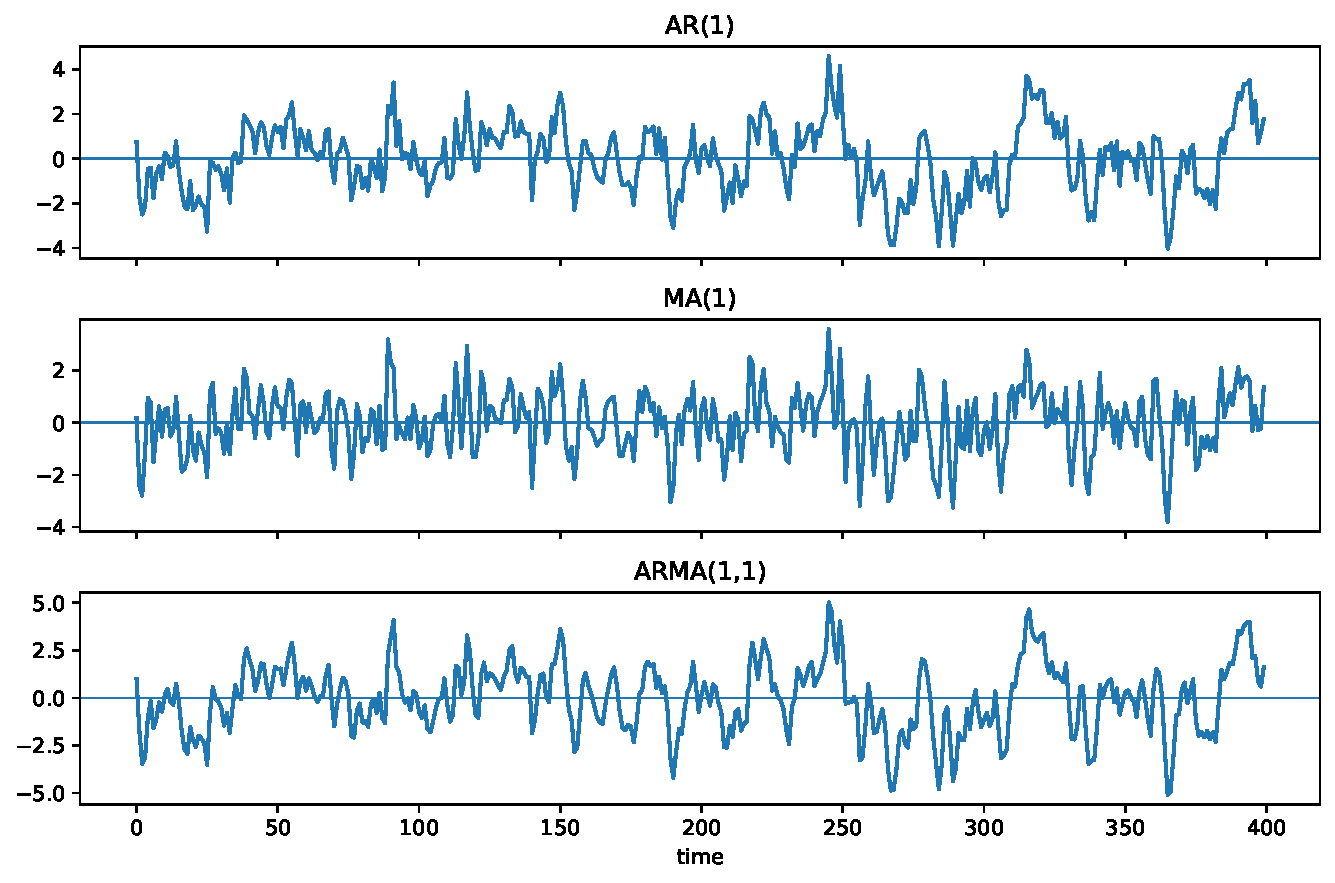
\includegraphics[keepaspectratio]{chapters/chapter-04-linear-processes-ar-ma-arma_files/figure-pdf/py-ch04-plot-simulated-processes-output-1.pdf}}

Even though all three processes are stationary in this example, they
have different dependence patterns. The AR(1) path often has persistent
runs above or below zero. The MA(1) path has shorter memory. The
ARMA(1,1) path combines both effects.

\section{4.18 Python example: sample ACF from
scratch}\label{python-example-sample-acf-from-scratch-1}

The sample ACF helps reveal dependence patterns.

\begin{Shaded}
\begin{Highlighting}[]
\ImportTok{import}\NormalTok{ numpy }\ImportTok{as}\NormalTok{ np}

\KeywordTok{def}\NormalTok{ sample\_acf(x, max\_lag):}
\NormalTok{    x }\OperatorTok{=}\NormalTok{ np.asarray(x)}
\NormalTok{    x }\OperatorTok{=}\NormalTok{ x }\OperatorTok{{-}}\NormalTok{ x.mean()}
\NormalTok{    denom }\OperatorTok{=}\NormalTok{ np.}\BuiltInTok{sum}\NormalTok{(x }\OperatorTok{*}\NormalTok{ x)}
\NormalTok{    acf }\OperatorTok{=}\NormalTok{ []}
    \ControlFlowTok{for}\NormalTok{ h }\KeywordTok{in} \BuiltInTok{range}\NormalTok{(max\_lag }\OperatorTok{+} \DecValTok{1}\NormalTok{):}
\NormalTok{        numer }\OperatorTok{=}\NormalTok{ np.}\BuiltInTok{sum}\NormalTok{(x[h:] }\OperatorTok{*}\NormalTok{ x[:}\BuiltInTok{len}\NormalTok{(x) }\OperatorTok{{-}}\NormalTok{ h])}
\NormalTok{        acf.append(numer }\OperatorTok{/}\NormalTok{ denom)}
    \ControlFlowTok{return}\NormalTok{ np.array(acf)}

\NormalTok{max\_lag }\OperatorTok{=} \DecValTok{30}
\NormalTok{acf\_table }\OperatorTok{=}\NormalTok{ pd.DataFrame(\{}
\NormalTok{    col: sample\_acf(series[col], max\_lag)}
    \ControlFlowTok{for}\NormalTok{ col }\KeywordTok{in}\NormalTok{ series.columns}
\NormalTok{\})}
\NormalTok{acf\_table.index.name }\OperatorTok{=} \StringTok{"lag"}
\NormalTok{acf\_table.head(}\DecValTok{10}\NormalTok{)}
\end{Highlighting}
\end{Shaded}

\protect\phantomsection\label{py-ch04-acf-from-scratch}
{\def\LTcaptype{none} % do not increment counter
\begin{longtable}[]{@{}llll@{}}
\toprule\noalign{}
& AR(1) & MA(1) & ARMA(1,1) \\
lag & & & \\
\midrule\noalign{}
\endhead
\bottomrule\noalign{}
\endlastfoot
0 & 1.000000 & 1.000000 & 1.000000 \\
1 & 0.759139 & 0.464328 & 0.808694 \\
2 & 0.595125 & 0.002913 & 0.550931 \\
3 & 0.476362 & 0.005060 & 0.397093 \\
4 & 0.396639 & 0.047589 & 0.315935 \\
5 & 0.348908 & 0.133573 & 0.271041 \\
6 & 0.275336 & 0.103624 & 0.203381 \\
7 & 0.187383 & -0.000791 & 0.121054 \\
8 & 0.131376 & -0.031386 & 0.066007 \\
9 & 0.094999 & -0.001828 & 0.040928 \\
\end{longtable}
}

\begin{Shaded}
\begin{Highlighting}[]
\NormalTok{fig, axes }\OperatorTok{=}\NormalTok{ plt.subplots(}\DecValTok{3}\NormalTok{, }\DecValTok{1}\NormalTok{, figsize}\OperatorTok{=}\NormalTok{(}\DecValTok{9}\NormalTok{, }\DecValTok{6}\NormalTok{), sharex}\OperatorTok{=}\VariableTok{True}\NormalTok{)}
\NormalTok{lags }\OperatorTok{=}\NormalTok{ np.arange(max\_lag }\OperatorTok{+} \DecValTok{1}\NormalTok{)}
\ControlFlowTok{for}\NormalTok{ ax, col }\KeywordTok{in} \BuiltInTok{zip}\NormalTok{(axes, series.columns):}
\NormalTok{    ax.stem(lags, acf\_table[col].values)}
\NormalTok{    ax.set\_title(}\SpecialStringTok{f"Sample ACF: }\SpecialCharTok{\{}\NormalTok{col}\SpecialCharTok{\}}\SpecialStringTok{"}\NormalTok{)}
\NormalTok{    ax.axhline(}\DecValTok{0}\NormalTok{, linewidth}\OperatorTok{=}\FloatTok{0.8}\NormalTok{)}
\NormalTok{plt.xlabel(}\StringTok{"lag"}\NormalTok{)}
\NormalTok{plt.tight\_layout()}
\NormalTok{plt.show()}
\end{Highlighting}
\end{Shaded}

\pandocbounded{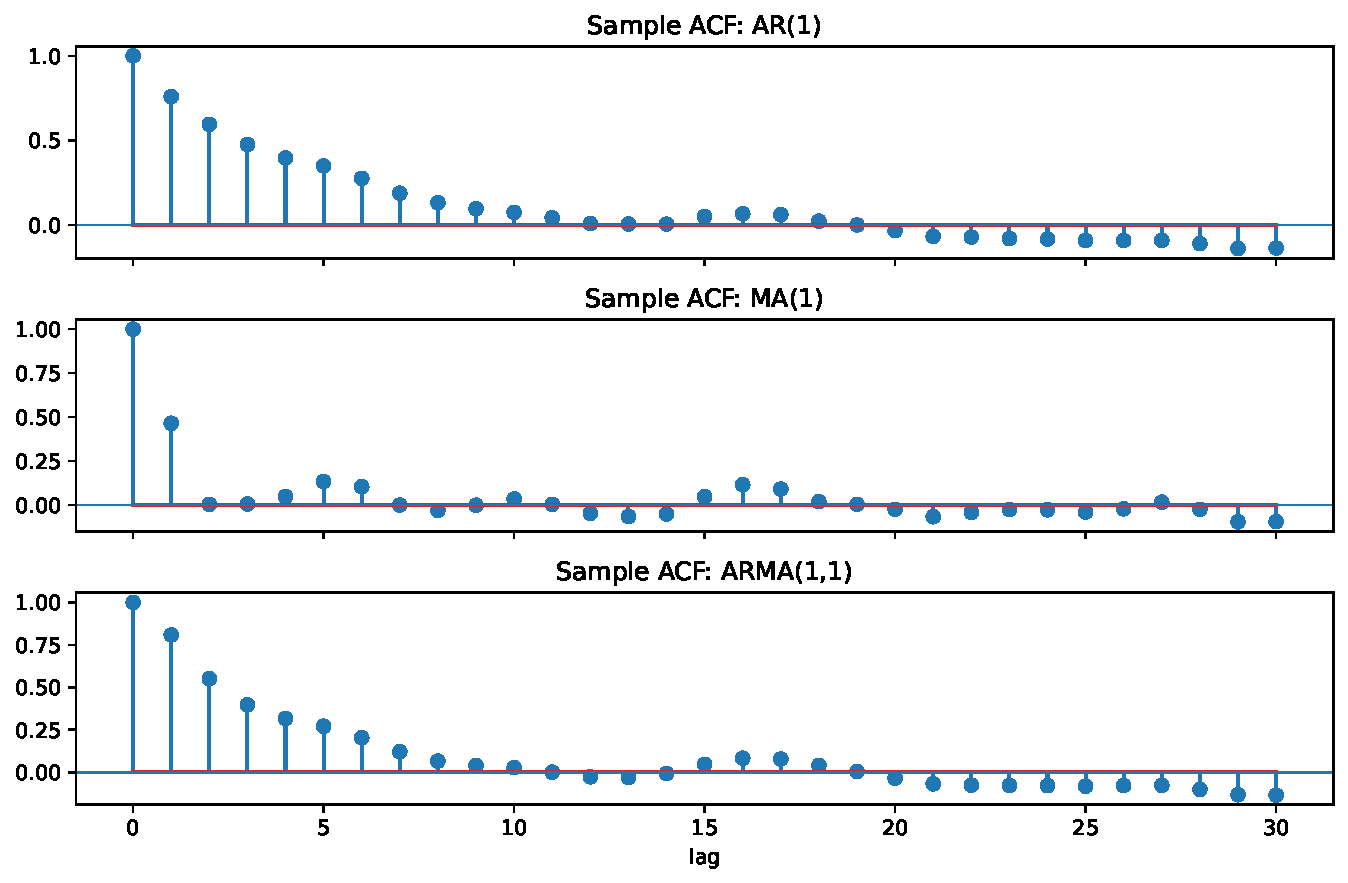
\includegraphics[keepaspectratio]{chapters/chapter-04-linear-processes-ar-ma-arma_files/figure-pdf/py-ch04-acf-plot-output-1.pdf}}

For the MA(1) process, the theoretical ACF is zero after lag \(1\), but
the sample ACF does not become exactly zero. This is sampling variation,
not necessarily model failure.

\section{4.19 Python example: root
checking}\label{python-example-root-checking}

AR and MA roots are central for causality and invertibility.

For an AR(\(p\)) model

\[
\phi(z)=1-\phi_1z-\cdots-\phi_pz^p.
\]

For an MA(\(q\)) model

\[
\theta(z)=1+\theta_1z+\cdots+\theta_qz^q.
\]

In Python, \texttt{numpy.roots} expects coefficients in descending
powers. The following helper functions compute roots of these
polynomials.

\protect\phantomsection\label{py-ch04-root-checking}
\begin{Shaded}
\begin{Highlighting}[]
\ImportTok{import}\NormalTok{ numpy }\ImportTok{as}\NormalTok{ np}

\KeywordTok{def}\NormalTok{ ar\_roots(phi):}
    \CommentTok{"""Roots of phi(z)=1{-}phi1 z{-}...{-}phip z\^{}p."""}
\NormalTok{    phi }\OperatorTok{=}\NormalTok{ np.asarray(phi, dtype}\OperatorTok{=}\BuiltInTok{float}\NormalTok{)}
\NormalTok{    coeff\_desc }\OperatorTok{=}\NormalTok{ np.r\_[}\OperatorTok{{-}}\NormalTok{phi[::}\OperatorTok{{-}}\DecValTok{1}\NormalTok{], }\FloatTok{1.0}\NormalTok{]}
    \ControlFlowTok{return}\NormalTok{ np.roots(coeff\_desc)}

\KeywordTok{def}\NormalTok{ ma\_roots(theta):}
    \CommentTok{"""Roots of theta(z)=1+theta1 z+...+thetaq z\^{}q."""}
\NormalTok{    theta }\OperatorTok{=}\NormalTok{ np.asarray(theta, dtype}\OperatorTok{=}\BuiltInTok{float}\NormalTok{)}
\NormalTok{    coeff\_desc }\OperatorTok{=}\NormalTok{ np.r\_[theta[::}\OperatorTok{{-}}\DecValTok{1}\NormalTok{], }\FloatTok{1.0}\NormalTok{]}
    \ControlFlowTok{return}\NormalTok{ np.roots(coeff\_desc)}

\KeywordTok{def}\NormalTok{ outside\_unit\_circle(roots, tol}\OperatorTok{=}\FloatTok{1e{-}10}\NormalTok{):}
    \ControlFlowTok{return}\NormalTok{ np.}\BuiltInTok{all}\NormalTok{(np.}\BuiltInTok{abs}\NormalTok{(roots) }\OperatorTok{\textgreater{}} \DecValTok{1} \OperatorTok{+}\NormalTok{ tol)}

\NormalTok{examples }\OperatorTok{=}\NormalTok{ \{}
    \StringTok{"AR(1), phi=0.75"}\NormalTok{: ar\_roots([}\FloatTok{0.75}\NormalTok{]),}
    \StringTok{"AR(1), phi=1.10"}\NormalTok{: ar\_roots([}\FloatTok{1.10}\NormalTok{]),}
    \StringTok{"MA(1), theta=0.70"}\NormalTok{: ma\_roots([}\FloatTok{0.70}\NormalTok{]),}
    \StringTok{"MA(1), theta=1.40"}\NormalTok{: ma\_roots([}\FloatTok{1.40}\NormalTok{]),}
\NormalTok{\}}

\ControlFlowTok{for}\NormalTok{ name, roots }\KeywordTok{in}\NormalTok{ examples.items():}
    \BuiltInTok{print}\NormalTok{(name)}
    \BuiltInTok{print}\NormalTok{(}\StringTok{"  roots:"}\NormalTok{, roots)}
    \BuiltInTok{print}\NormalTok{(}\StringTok{"  moduli:"}\NormalTok{, np.}\BuiltInTok{abs}\NormalTok{(roots))}
    \BuiltInTok{print}\NormalTok{(}\StringTok{"  outside unit circle:"}\NormalTok{, outside\_unit\_circle(roots))}
\end{Highlighting}
\end{Shaded}

\begin{verbatim}
AR(1), phi=0.75
  roots: [1.33333333]
  moduli: [1.33333333]
  outside unit circle: True
AR(1), phi=1.10
  roots: [0.90909091]
  moduli: [0.90909091]
  outside unit circle: False
MA(1), theta=0.70
  roots: [-1.42857143]
  moduli: [1.42857143]
  outside unit circle: True
MA(1), theta=1.40
  roots: [-0.71428571]
  moduli: [0.71428571]
  outside unit circle: False
\end{verbatim}

Interpretation:

\begin{itemize}
\tightlist
\item
  AR roots outside the unit circle imply causality.
\item
  MA roots outside the unit circle imply invertibility.
\item
  Roots near the unit circle imply slow decay and numerical sensitivity.
\end{itemize}

\section{\texorpdfstring{4.20 Python example: compute \(\psi\)-weights
recursively}{4.20 Python example: compute \textbackslash psi-weights recursively}}\label{python-example-compute-psi-weights-recursively}

The following function computes the causal impulse-response coefficients
of an ARMA model by matching coefficients in

\[
\phi(B)\psi(B)=\theta(B).
\]

\begin{Shaded}
\begin{Highlighting}[]
\ImportTok{import}\NormalTok{ numpy }\ImportTok{as}\NormalTok{ np}

\KeywordTok{def}\NormalTok{ psi\_weights(ar}\OperatorTok{=}\VariableTok{None}\NormalTok{, ma}\OperatorTok{=}\VariableTok{None}\NormalTok{, horizon}\OperatorTok{=}\DecValTok{30}\NormalTok{):}
    \CommentTok{"""}
\CommentTok{    Compute psi\_0,...,psi\_horizon for}
\CommentTok{    phi(B) X\_t = theta(B) W\_t,}
\CommentTok{    phi(B)=1 {-} ar[0]B {-} ...,}
\CommentTok{    theta(B)=1 + ma[0]B + ... .}
\CommentTok{    """}
\NormalTok{    ar }\OperatorTok{=}\NormalTok{ np.asarray([] }\ControlFlowTok{if}\NormalTok{ ar }\KeywordTok{is} \VariableTok{None} \ControlFlowTok{else}\NormalTok{ ar, dtype}\OperatorTok{=}\BuiltInTok{float}\NormalTok{)}
\NormalTok{    ma }\OperatorTok{=}\NormalTok{ np.asarray([] }\ControlFlowTok{if}\NormalTok{ ma }\KeywordTok{is} \VariableTok{None} \ControlFlowTok{else}\NormalTok{ ma, dtype}\OperatorTok{=}\BuiltInTok{float}\NormalTok{)}
\NormalTok{    p }\OperatorTok{=} \BuiltInTok{len}\NormalTok{(ar)}
\NormalTok{    q }\OperatorTok{=} \BuiltInTok{len}\NormalTok{(ma)}
\NormalTok{    psi }\OperatorTok{=}\NormalTok{ np.zeros(horizon }\OperatorTok{+} \DecValTok{1}\NormalTok{)}
\NormalTok{    psi[}\DecValTok{0}\NormalTok{] }\OperatorTok{=} \FloatTok{1.0}
    \ControlFlowTok{for}\NormalTok{ k }\KeywordTok{in} \BuiltInTok{range}\NormalTok{(}\DecValTok{1}\NormalTok{, horizon }\OperatorTok{+} \DecValTok{1}\NormalTok{):}
\NormalTok{        theta\_k }\OperatorTok{=}\NormalTok{ ma[k }\OperatorTok{{-}} \DecValTok{1}\NormalTok{] }\ControlFlowTok{if}\NormalTok{ k }\OperatorTok{\textless{}=}\NormalTok{ q }\ControlFlowTok{else} \FloatTok{0.0}
\NormalTok{        ar\_part }\OperatorTok{=} \FloatTok{0.0}
        \ControlFlowTok{for}\NormalTok{ j }\KeywordTok{in} \BuiltInTok{range}\NormalTok{(}\DecValTok{1}\NormalTok{, p }\OperatorTok{+} \DecValTok{1}\NormalTok{):}
            \ControlFlowTok{if}\NormalTok{ k }\OperatorTok{{-}}\NormalTok{ j }\OperatorTok{\textgreater{}=} \DecValTok{0}\NormalTok{:}
\NormalTok{                ar\_part }\OperatorTok{+=}\NormalTok{ ar[j }\OperatorTok{{-}} \DecValTok{1}\NormalTok{] }\OperatorTok{*}\NormalTok{ psi[k }\OperatorTok{{-}}\NormalTok{ j]}
\NormalTok{        psi[k] }\OperatorTok{=}\NormalTok{ theta\_k }\OperatorTok{+}\NormalTok{ ar\_part}
    \ControlFlowTok{return}\NormalTok{ psi}

\NormalTok{psi\_ar1 }\OperatorTok{=}\NormalTok{ psi\_weights(ar}\OperatorTok{=}\NormalTok{[}\FloatTok{0.75}\NormalTok{], ma}\OperatorTok{=}\NormalTok{[], horizon}\OperatorTok{=}\DecValTok{20}\NormalTok{)}
\NormalTok{psi\_ma1 }\OperatorTok{=}\NormalTok{ psi\_weights(ar}\OperatorTok{=}\NormalTok{[], ma}\OperatorTok{=}\NormalTok{[}\FloatTok{0.70}\NormalTok{], horizon}\OperatorTok{=}\DecValTok{20}\NormalTok{)}
\NormalTok{psi\_arma11 }\OperatorTok{=}\NormalTok{ psi\_weights(ar}\OperatorTok{=}\NormalTok{[}\FloatTok{0.65}\NormalTok{], ma}\OperatorTok{=}\NormalTok{[}\FloatTok{0.50}\NormalTok{], horizon}\OperatorTok{=}\DecValTok{20}\NormalTok{)}

\NormalTok{pd.DataFrame(\{}
    \StringTok{"lag"}\NormalTok{: np.arange(}\DecValTok{21}\NormalTok{),}
    \StringTok{"AR(1) psi"}\NormalTok{: psi\_ar1,}
    \StringTok{"MA(1) psi"}\NormalTok{: psi\_ma1,}
    \StringTok{"ARMA(1,1) psi"}\NormalTok{: psi\_arma11}
\NormalTok{\}).head(}\DecValTok{12}\NormalTok{)}
\end{Highlighting}
\end{Shaded}

\protect\phantomsection\label{py-ch04-psi-weights}
{\def\LTcaptype{none} % do not increment counter
\begin{longtable}[]{@{}lllll@{}}
\toprule\noalign{}
& lag & AR(1) psi & MA(1) psi & ARMA(1,1) psi \\
\midrule\noalign{}
\endhead
\bottomrule\noalign{}
\endlastfoot
0 & 0 & 1.000000 & 1.0 & 1.000000 \\
1 & 1 & 0.750000 & 0.7 & 1.150000 \\
2 & 2 & 0.562500 & 0.0 & 0.747500 \\
3 & 3 & 0.421875 & 0.0 & 0.485875 \\
4 & 4 & 0.316406 & 0.0 & 0.315819 \\
5 & 5 & 0.237305 & 0.0 & 0.205282 \\
6 & 6 & 0.177979 & 0.0 & 0.133433 \\
7 & 7 & 0.133484 & 0.0 & 0.086732 \\
8 & 8 & 0.100113 & 0.0 & 0.056376 \\
9 & 9 & 0.075085 & 0.0 & 0.036644 \\
10 & 10 & 0.056314 & 0.0 & 0.023819 \\
11 & 11 & 0.042235 & 0.0 & 0.015482 \\
\end{longtable}
}

\begin{Shaded}
\begin{Highlighting}[]
\NormalTok{fig, ax }\OperatorTok{=}\NormalTok{ plt.subplots(figsize}\OperatorTok{=}\NormalTok{(}\DecValTok{9}\NormalTok{, }\DecValTok{4}\NormalTok{))}
\NormalTok{ax.plot(psi\_ar1, marker}\OperatorTok{=}\StringTok{"o"}\NormalTok{, label}\OperatorTok{=}\StringTok{"AR(1)"}\NormalTok{)}
\NormalTok{ax.plot(psi\_ma1, marker}\OperatorTok{=}\StringTok{"o"}\NormalTok{, label}\OperatorTok{=}\StringTok{"MA(1)"}\NormalTok{)}
\NormalTok{ax.plot(psi\_arma11, marker}\OperatorTok{=}\StringTok{"o"}\NormalTok{, label}\OperatorTok{=}\StringTok{"ARMA(1,1)"}\NormalTok{)}
\NormalTok{ax.axhline(}\DecValTok{0}\NormalTok{, linewidth}\OperatorTok{=}\FloatTok{0.8}\NormalTok{)}
\NormalTok{ax.set\_xlabel(}\StringTok{"lag j"}\NormalTok{)}
\NormalTok{ax.set\_ylabel(}\StringTok{"psi\_j"}\NormalTok{)}
\NormalTok{ax.set\_title(}\StringTok{"Impulse{-}response weights"}\NormalTok{)}
\NormalTok{ax.legend()}
\NormalTok{plt.show()}
\end{Highlighting}
\end{Shaded}

\pandocbounded{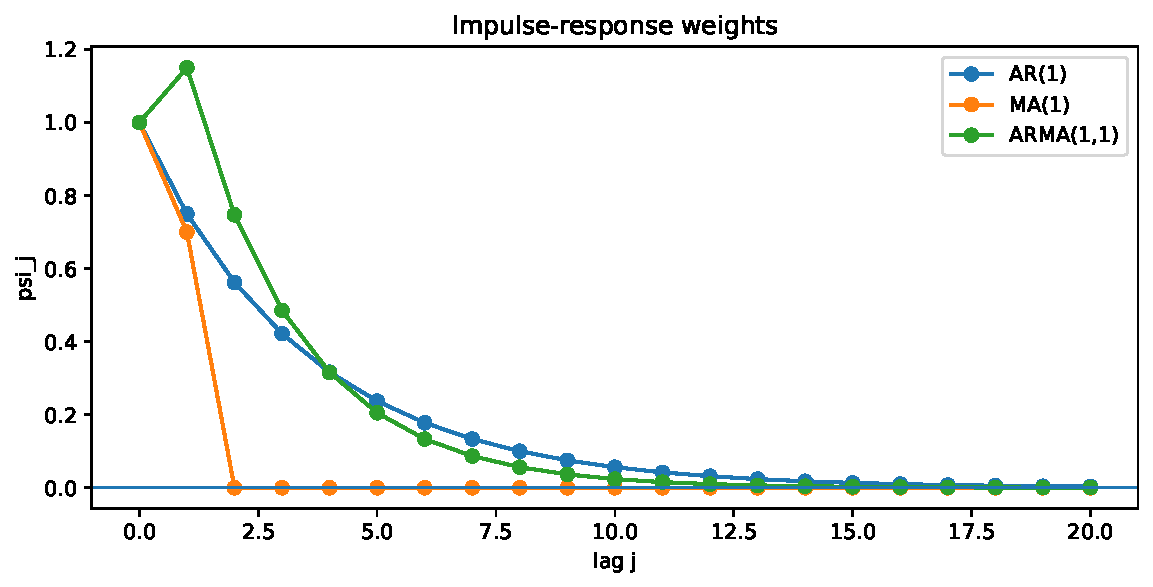
\includegraphics[keepaspectratio]{chapters/chapter-04-linear-processes-ar-ma-arma_files/figure-pdf/py-ch04-psi-plot-output-1.pdf}}

The MA(1) impulse response cuts off immediately after lag \(1\). The
AR(1) impulse response decays geometrically. The ARMA(1,1) impulse
response has a first coefficient affected by the MA term, then decays
according to the AR coefficient.

\section{\texorpdfstring{4.21 Python example: autocovariance from
\(\psi\)-weights}{4.21 Python example: autocovariance from \textbackslash psi-weights}}\label{python-example-autocovariance-from-psi-weights}

For a causal linear process,

\[
\gamma(h)=\sigma^2\sum_{j=0}^{\infty}\psi_j\psi_{j+h}.
\]

The following function approximates this by truncating the \(\psi\)
sequence.

\begin{Shaded}
\begin{Highlighting}[]
\KeywordTok{def}\NormalTok{ acf\_from\_psi(psi, max\_lag, sigma2}\OperatorTok{=}\FloatTok{1.0}\NormalTok{):}
\NormalTok{    psi }\OperatorTok{=}\NormalTok{ np.asarray(psi, dtype}\OperatorTok{=}\BuiltInTok{float}\NormalTok{)}
\NormalTok{    gamma }\OperatorTok{=}\NormalTok{ []}
    \ControlFlowTok{for}\NormalTok{ h }\KeywordTok{in} \BuiltInTok{range}\NormalTok{(max\_lag }\OperatorTok{+} \DecValTok{1}\NormalTok{):}
\NormalTok{        gamma\_h }\OperatorTok{=}\NormalTok{ sigma2 }\OperatorTok{*}\NormalTok{ np.}\BuiltInTok{sum}\NormalTok{(psi[:}\BuiltInTok{len}\NormalTok{(psi) }\OperatorTok{{-}}\NormalTok{ h] }\OperatorTok{*}\NormalTok{ psi[h:])}
\NormalTok{        gamma.append(gamma\_h)}
\NormalTok{    gamma }\OperatorTok{=}\NormalTok{ np.array(gamma)}
    \ControlFlowTok{return}\NormalTok{ gamma }\OperatorTok{/}\NormalTok{ gamma[}\DecValTok{0}\NormalTok{]}

\NormalTok{long\_psi\_ar1 }\OperatorTok{=}\NormalTok{ psi\_weights(ar}\OperatorTok{=}\NormalTok{[}\FloatTok{0.75}\NormalTok{], horizon}\OperatorTok{=}\DecValTok{300}\NormalTok{)}
\NormalTok{acf\_ar1\_approx }\OperatorTok{=}\NormalTok{ acf\_from\_psi(long\_psi\_ar1, max\_lag}\OperatorTok{=}\DecValTok{20}\NormalTok{)}
\NormalTok{acf\_ar1\_exact }\OperatorTok{=} \FloatTok{0.75} \OperatorTok{**}\NormalTok{ np.arange(}\DecValTok{21}\NormalTok{)}

\NormalTok{pd.DataFrame(\{}
    \StringTok{"lag"}\NormalTok{: np.arange(}\DecValTok{21}\NormalTok{),}
    \StringTok{"approx from psi"}\NormalTok{: acf\_ar1\_approx,}
    \StringTok{"exact AR(1)"}\NormalTok{: acf\_ar1\_exact}
\NormalTok{\}).head(}\DecValTok{10}\NormalTok{)}
\end{Highlighting}
\end{Shaded}

\protect\phantomsection\label{py-ch04-autocov-from-psi}
{\def\LTcaptype{none} % do not increment counter
\begin{longtable}[]{@{}llll@{}}
\toprule\noalign{}
& lag & approx from psi & exact AR(1) \\
\midrule\noalign{}
\endhead
\bottomrule\noalign{}
\endlastfoot
0 & 0 & 1.000000 & 1.000000 \\
1 & 1 & 0.750000 & 0.750000 \\
2 & 2 & 0.562500 & 0.562500 \\
3 & 3 & 0.421875 & 0.421875 \\
4 & 4 & 0.316406 & 0.316406 \\
5 & 5 & 0.237305 & 0.237305 \\
6 & 6 & 0.177979 & 0.177979 \\
7 & 7 & 0.133484 & 0.133484 \\
8 & 8 & 0.100113 & 0.100113 \\
9 & 9 & 0.075085 & 0.075085 \\
\end{longtable}
}

The approximation matches the exact AR(1) ACF very closely because the
impulse response decays geometrically.

\section{\texorpdfstring{4.22 Python example: fitting ARMA models with
\texttt{statsmodels}}{4.22 Python example: fitting ARMA models with statsmodels}}\label{python-example-fitting-arma-models-with-statsmodels}

In practice we estimate ARMA models from data. In \texttt{statsmodels},
ARMA models are often fit using the ARIMA class with
\texttt{order=(p,0,q)}.

\protect\phantomsection\label{py-ch04-fit-arma}
\begin{Shaded}
\begin{Highlighting}[]
\ImportTok{from}\NormalTok{ statsmodels.tsa.arima.model }\ImportTok{import}\NormalTok{ ARIMA}

\CommentTok{\# Fit ARMA(1,1) to the simulated ARMA(1,1) data}
\NormalTok{fit }\OperatorTok{=}\NormalTok{ ARIMA(x\_arma11, order}\OperatorTok{=}\NormalTok{(}\DecValTok{1}\NormalTok{, }\DecValTok{0}\NormalTok{, }\DecValTok{1}\NormalTok{), trend}\OperatorTok{=}\StringTok{"n"}\NormalTok{).fit()}
\BuiltInTok{print}\NormalTok{(fit.summary())}
\end{Highlighting}
\end{Shaded}

\begin{verbatim}
                               SARIMAX Results                                
==============================================================================
Dep. Variable:                      y   No. Observations:                  400
Model:                 ARIMA(1, 0, 1)   Log Likelihood                -565.474
Date:                Fri, 19 Jun 2026   AIC                           1136.949
Time:                        19:56:57   BIC                           1148.923
Sample:                             0   HQIC                          1141.691
                                - 400                                         
Covariance Type:                  opg                                         
==============================================================================
                 coef    std err          z      P>|z|      [0.025      0.975]
------------------------------------------------------------------------------
ar.L1          0.6657      0.046     14.601      0.000       0.576       0.755
ma.L1          0.4744      0.055      8.668      0.000       0.367       0.582
sigma2         0.9861      0.067     14.707      0.000       0.855       1.118
===================================================================================
Ljung-Box (L1) (Q):                   0.04   Jarque-Bera (JB):                 0.70
Prob(Q):                              0.83   Prob(JB):                         0.70
Heteroskedasticity (H):               1.17   Skew:                             0.06
Prob(H) (two-sided):                  0.38   Kurtosis:                         3.17
===================================================================================

Warnings:
[1] Covariance matrix calculated using the outer product of gradients (complex-step).
\end{verbatim}

Residual diagnostics are essential.

\begin{Shaded}
\begin{Highlighting}[]
\NormalTok{resid }\OperatorTok{=}\NormalTok{ fit.resid}
\NormalTok{resid\_acf }\OperatorTok{=}\NormalTok{ sample\_acf(resid, }\DecValTok{25}\NormalTok{)}

\NormalTok{fig, axes }\OperatorTok{=}\NormalTok{ plt.subplots(}\DecValTok{2}\NormalTok{, }\DecValTok{1}\NormalTok{, figsize}\OperatorTok{=}\NormalTok{(}\DecValTok{9}\NormalTok{, }\DecValTok{5}\NormalTok{))}
\NormalTok{axes[}\DecValTok{0}\NormalTok{].plot(resid)}
\NormalTok{axes[}\DecValTok{0}\NormalTok{].axhline(}\DecValTok{0}\NormalTok{, linewidth}\OperatorTok{=}\FloatTok{0.8}\NormalTok{)}
\NormalTok{axes[}\DecValTok{0}\NormalTok{].set\_title(}\StringTok{"Residuals from fitted ARMA(1,1)"}\NormalTok{)}
\NormalTok{axes[}\DecValTok{1}\NormalTok{].stem(np.arange(}\DecValTok{26}\NormalTok{), resid\_acf)}
\NormalTok{axes[}\DecValTok{1}\NormalTok{].axhline(}\DecValTok{0}\NormalTok{, linewidth}\OperatorTok{=}\FloatTok{0.8}\NormalTok{)}
\NormalTok{axes[}\DecValTok{1}\NormalTok{].set\_title(}\StringTok{"Residual ACF"}\NormalTok{)}
\NormalTok{axes[}\DecValTok{1}\NormalTok{].set\_xlabel(}\StringTok{"lag"}\NormalTok{)}
\NormalTok{plt.tight\_layout()}
\NormalTok{plt.show()}
\end{Highlighting}
\end{Shaded}

\pandocbounded{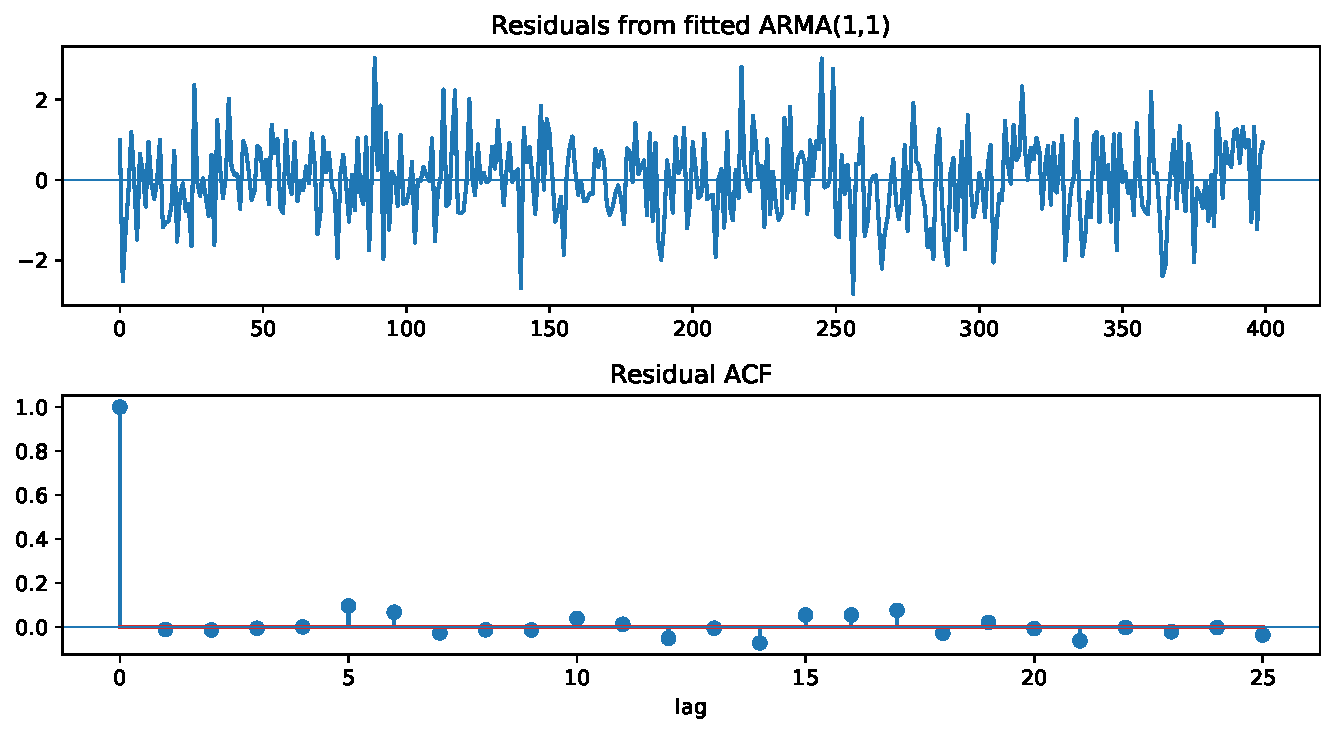
\includegraphics[keepaspectratio]{chapters/chapter-04-linear-processes-ar-ma-arma_files/figure-pdf/py-ch04-residual-diagnostics-output-1.pdf}}

If the fitted model captures the dependence, the residual ACF should
look approximately like white noise.

\section{4.23 Python example: compare candidate model
orders}\label{python-example-compare-candidate-model-orders}

Information criteria provide one way to compare ARMA orders. The
following code fits several small ARMA models and reports AIC and BIC.

\begin{Shaded}
\begin{Highlighting}[]
\NormalTok{results }\OperatorTok{=}\NormalTok{ []}
\ControlFlowTok{for}\NormalTok{ p }\KeywordTok{in} \BuiltInTok{range}\NormalTok{(}\DecValTok{4}\NormalTok{):}
    \ControlFlowTok{for}\NormalTok{ q }\KeywordTok{in} \BuiltInTok{range}\NormalTok{(}\DecValTok{4}\NormalTok{):}
        \ControlFlowTok{if}\NormalTok{ p }\OperatorTok{==} \DecValTok{0} \KeywordTok{and}\NormalTok{ q }\OperatorTok{==} \DecValTok{0}\NormalTok{:}
            \ControlFlowTok{continue}
        \ControlFlowTok{try}\NormalTok{:}
\NormalTok{            model }\OperatorTok{=}\NormalTok{ ARIMA(x\_arma11, order}\OperatorTok{=}\NormalTok{(p, }\DecValTok{0}\NormalTok{, q), trend}\OperatorTok{=}\StringTok{"n"}\NormalTok{).fit()}
\NormalTok{            results.append(\{}
                \StringTok{"p"}\NormalTok{: p,}
                \StringTok{"q"}\NormalTok{: q,}
                \StringTok{"aic"}\NormalTok{: model.aic,}
                \StringTok{"bic"}\NormalTok{: model.bic}
\NormalTok{            \})}
        \ControlFlowTok{except} \PreprocessorTok{Exception} \ImportTok{as}\NormalTok{ err:}
\NormalTok{            results.append(\{}
                \StringTok{"p"}\NormalTok{: p,}
                \StringTok{"q"}\NormalTok{: q,}
                \StringTok{"aic"}\NormalTok{: np.nan,}
                \StringTok{"bic"}\NormalTok{: np.nan}
\NormalTok{            \})}

\NormalTok{order\_table }\OperatorTok{=}\NormalTok{ pd.DataFrame(results).sort\_values(}\StringTok{"aic"}\NormalTok{)}
\NormalTok{order\_table.head(}\DecValTok{10}\NormalTok{)}
\end{Highlighting}
\end{Shaded}

\protect\phantomsection\label{py-ch04-model-order-grid}
{\def\LTcaptype{none} % do not increment counter
\begin{longtable}[]{@{}lllll@{}}
\toprule\noalign{}
& p & q & aic & bic \\
\midrule\noalign{}
\endhead
\bottomrule\noalign{}
\endlastfoot
4 & 1 & 1 & 1136.948542 & 1148.922936 \\
9 & 2 & 2 & 1138.404450 & 1158.361772 \\
11 & 3 & 0 & 1138.505188 & 1154.471046 \\
5 & 1 & 2 & 1138.637464 & 1154.603322 \\
8 & 2 & 1 & 1138.690447 & 1154.656305 \\
14 & 3 & 3 & 1139.601729 & 1167.541981 \\
6 & 1 & 3 & 1140.125820 & 1160.083142 \\
12 & 3 & 1 & 1140.375193 & 1160.332516 \\
13 & 3 & 2 & 1141.443823 & 1165.392610 \\
10 & 2 & 3 & 1141.649769 & 1165.598557 \\
\end{longtable}
}

This grid is not a substitute for diagnosis. A model with low AIC can
still have residual autocorrelation, unstable parameters, or poor
forecasting performance.

\section{4.24 Connection to machine
learning}\label{connection-to-machine-learning}

ARMA models can be viewed as a simple and interpretable machine-learning
architecture for sequential data.

\subsection{AR as linear supervised learning on lag
features}\label{ar-as-linear-supervised-learning-on-lag-features}

An AR(\(p\)) model is

\[
X_t=\phi_1X_{t-1}+\cdots+\phi_pX_{t-p}+W_t.
\]

This is linear regression with features

\[
(X_{t-1},X_{t-2},\dots,X_{t-p}).
\]

The difference from ordinary regression is that the features are
generated from the same dependent time series, so validation and
uncertainty require time-series methods.

\subsection{MA as latent-shock
modeling}\label{ma-as-latent-shock-modeling}

An MA(\(q\)) model uses unobserved shocks:

\[
X_t=W_t+\theta_1W_{t-1}+\cdots+\theta_qW_{t-q}.
\]

The predictors \(W_{t-j}\) are not directly observed. They must be
inferred through model fitting.

\subsection{ARMA as a linear recurrent
system}\label{arma-as-a-linear-recurrent-system}

An ARMA model combines recurrence through \(X_{t-j}\) and shock
filtering through \(W_{t-j}\). This makes it an ancestor of modern
sequence models: it has hidden memory, impulse responses, and recursive
prediction. RNNs, LSTMs, temporal convolutional networks, and
state-space sequence models generalize these ideas in nonlinear and
high-dimensional ways.

\section{AI connection}\label{ai-connection}

A modern AI model may learn complex nonlinear sequence representations,
but the same questions remain:

\begin{itemize}
\tightlist
\item
  What past information matters?
\item
  How long does memory persist?
\item
  Are residuals still dependent?
\item
  Is the model stable when rolled forward?
\item
  Does it generalize under time-aware validation?
\end{itemize}

ARMA models give a mathematically transparent setting for learning these
questions before moving to deep models.

\section{4.25 Common mistakes}\label{common-mistakes-3}

\subsection{Mistake 1: confusing stationarity with
causality}\label{mistake-1-confusing-stationarity-with-causality}

A stationary solution may exist even when the model is not causal. For
forecasting, we usually need a causal representation because we cannot
use future shocks.

\subsection{Mistake 2: forgetting
invertibility}\label{mistake-2-forgetting-invertibility}

An MA model can be stationary for any parameter value, but not every
parameter value gives a unique and stable innovation representation.
Invertibility is needed for canonical estimation and interpretation.

\subsection{Mistake 3: treating AR and MA roots the same way without
checking
signs}\label{mistake-3-treating-ar-and-ma-roots-the-same-way-without-checking-signs}

AR and MA polynomials are written with different sign conventions:

\[
\phi(z)=1-\phi_1z-\cdots-\phi_pz^p,
\]

while

\[
\theta(z)=1+\theta_1z+\cdots+\theta_qz^q.
\]

When coding root checks, pay close attention to the coefficient order
and signs.

\subsection{Mistake 4: believing sample ACF cutoffs are
exact}\label{mistake-4-believing-sample-acf-cutoffs-are-exact}

The theoretical ACF of MA(\(q\)) cuts off. The sample ACF only
fluctuates around zero after lag \(q\).

\subsection{Mistake 5: fitting ARMA to nonstationary
data}\label{mistake-5-fitting-arma-to-nonstationary-data}

ARMA models are for stationary data. If the time plot or ACF suggests
trend, seasonality, or changing variance, consider transformation,
detrending, differencing, ARIMA, SARIMA, or another model class.

\section{4.26 AI-assisted modeling
activities}\label{ai-assisted-modeling-activities}

AI tools are useful for this chapter because there is a lot of algebra.
They are also risky because a small sign mistake changes the model.

\subsection{Prompt 1: root conditions}\label{prompt-1-root-conditions}

\begin{quote}
I have the model \((1-0.6B+0.1B^2)X_t=(1+0.4B)W_t\). Explain how to
check causality and invertibility. Show the polynomial roots and
interpret whether they are outside the unit circle.
\end{quote}

Verification steps:

\begin{enumerate}
\def\labelenumi{\arabic{enumi}.}
\tightlist
\item
  Identify the AR polynomial \(\phi(z)=1-0.6z+0.1z^2\).
\item
  Identify the MA polynomial \(\theta(z)=1+0.4z\).
\item
  Compute roots numerically.
\item
  Check moduli.
\item
  State causal and invertible conclusions separately.
\end{enumerate}

\subsection{Prompt 2: impulse-response
coefficients}\label{prompt-2-impulse-response-coefficients}

\begin{quote}
Derive the first six \(\psi\)-weights for the ARMA(1,1) model
\((1-\phi B)X_t=(1+\theta B)W_t\).
\end{quote}

A correct answer should give

\[
\psi_0=1,
\]

\[
\psi_1=\phi+\theta,
\]

and

\[
\psi_k=\phi\psi_{k-1}\quad(k\ge2).
\]

\subsection{Prompt 3: code audit}\label{prompt-3-code-audit}

\begin{quote}
The following Python function is supposed to compute AR roots. Check
whether the coefficient signs and ordering are correct for
\(\phi(z)=1-\phi_1z-\cdots-\phi_pz^p\).
\end{quote}

Ask the AI to explain its reasoning, then test the function on AR(1),
where the root is known to be \(1/\phi\).

\subsection{Prompt 4: model
interpretation}\label{prompt-4-model-interpretation}

\begin{quote}
I fitted an ARMA(2,1) model and obtained roots close to the unit circle.
What does that mean for forecasting, impulse responses, and numerical
stability?
\end{quote}

A good answer should mention slow decay, possible near-nonstationarity,
larger forecast uncertainty, sensitivity to sample variation, and the
need for residual and rolling forecast diagnostics.

\begin{tcolorbox}[enhanced jigsaw, arc=.35mm, bottomrule=.15mm, bottomtitle=1mm, breakable, colback=white, colbacktitle=quarto-callout-warning-color!10!white, colframe=quarto-callout-warning-color-frame, coltitle=black, left=2mm, leftrule=.75mm, opacityback=0, opacitybacktitle=0.6, rightrule=.15mm, title=\textcolor{quarto-callout-warning-color}{\faExclamationTriangle}\hspace{0.5em}{AI safety rule for ARMA algebra}, titlerule=0mm, toprule=.15mm, toptitle=1mm]

Always test AI-generated formulas on AR(1) or MA(1), where you know the
answer. If the formula fails the simple case, do not trust it for
ARMA(\(p,q\)).

\end{tcolorbox}

\section{4.27 Mini project: ARMA process
laboratory}\label{mini-project-arma-process-laboratory}

Create a short ARMA modeling report using either simulated data or a
real stationary time series.

Your report should include:

\begin{enumerate}
\def\labelenumi{\arabic{enumi}.}
\tightlist
\item
  \textbf{Data description.} What is the series? What is the time unit?
\item
  \textbf{Stationarity check.} Show a time plot and sample ACF.
\item
  \textbf{Candidate models.} Try at least three ARMA\((p,q)\)
  specifications.
\item
  \textbf{Root checks.} For each fitted model, report AR and MA roots
  and say whether they satisfy the usual conditions.
\item
  \textbf{Residual diagnostics.} Plot residuals and residual ACF.
\item
  \textbf{Forecast comparison.} Compare one-step or multi-step forecast
  errors on a held-out time block.
\item
  \textbf{Interpretation.} Explain the chosen model in terms of memory
  and shocks.
\item
  \textbf{AI reflection.} Ask an AI assistant to critique your model
  choice. Include the critique and your response.
\end{enumerate}

\section{4.28 Exercises}\label{exercises-3}

\subsection{Conceptual exercises}\label{conceptual-exercises-3}

\begin{enumerate}
\def\labelenumi{\arabic{enumi}.}
\tightlist
\item
  Define the backshift operator \(B\) and compute \((1-B)^2X_t\).
\item
  Explain the difference between an AR(\(p\)) model and an MA(\(q\))
  model.
\item
  Explain why an MA(\(q\)) model is always weakly stationary.
\item
  Explain why a causal AR(1) process has infinitely many MA
  coefficients.
\item
  Define causality and invertibility in words.
\item
  Explain why the roots of \(\phi(z)\) control causality.
\item
  Explain why the roots of \(\theta(z)\) control invertibility.
\item
  Explain why common factors in \(\phi(B)\) and \(\theta(B)\) create
  parameter redundancy.
\item
  Describe the ACF signature of an MA(\(q\)) model.
\item
  Describe the ACF and PACF signatures of an AR(\(p\)) model.
\end{enumerate}

\subsection{Mathematical exercises}\label{mathematical-exercises-2}

\begin{enumerate}
\def\labelenumi{\arabic{enumi}.}
\setcounter{enumi}{10}
\tightlist
\item
  For MA(1), derive \(\gamma(0)\), \(\gamma(1)\), and \(\rho(1)\).
\item
  Show that \(\theta\) and \(1/\theta\) give the same lag-one ACF for
  MA(1).
\item
  For AR(1), show that \(|\phi|<1\) is equivalent to the AR root being
  outside the unit circle.
\item
  For AR(1), derive the causal representation
  \(X_t=\sum_{j=0}^{\infty}\phi^jW_{t-j}\).
\item
  For AR(1), derive \(\gamma(0)=\sigma^2/(1-\phi^2)\).
\item
  For AR(1), derive \(\rho(h)=\phi^{|h|}\).
\item
  For ARMA(1,1), derive \(\psi_0,\psi_1,\psi_2,\psi_3\).
\item
  For AR(2), use coefficient matching to find \(\psi_0,\dots,\psi_5\) in
  terms of \(\phi_1\) and \(\phi_2\).
\item
  Let \(\phi(z)=1-1.2z+0.35z^2\). Compute the roots and determine
  whether the AR(2) model is causal.
\item
  Let \(\theta(z)=1+1.5z\). Determine whether the corresponding MA(1)
  model is invertible.
\end{enumerate}

\subsection{Python exercises}\label{python-exercises-1}

\begin{enumerate}
\def\labelenumi{\arabic{enumi}.}
\setcounter{enumi}{20}
\tightlist
\item
  Write a function that simulates an AR(\(p\)) process from a vector of
  AR coefficients.
\item
  Write a function that simulates an MA(\(q\)) process from a vector of
  MA coefficients.
\item
  Write a function that computes AR roots and checks whether they are
  outside the unit circle.
\item
  Write a function that computes MA roots and checks whether they are
  outside the unit circle.
\item
  Simulate AR(1) processes with \(\phi=0.2\), \(0.8\), \(-0.8\), and
  \(1.0\). Compare the time plots and ACFs.
\item
  Simulate MA(1) processes with \(\theta=0.5\) and \(\theta=2.0\).
  Compare their sample ACFs and discuss invertibility.
\item
  Simulate an ARMA(1,1) model and estimate it using
  \texttt{statsmodels}.
\item
  Fit several ARMA models to the same series and compare AIC, BIC,
  residual ACF, and forecast error.
\item
  Use the \(\psi\)-weight recursion to approximate the ACF of an
  ARMA(1,1) model.
\item
  Create a near-unit-root AR(1) process with \(\phi=0.98\) and discuss
  why it can be hard to distinguish from nonstationarity in finite
  samples.
\end{enumerate}

\subsection{AI-assisted exercises}\label{ai-assisted-exercises-1}

\begin{enumerate}
\def\labelenumi{\arabic{enumi}.}
\setcounter{enumi}{30}
\tightlist
\item
  Ask an AI assistant to derive the AR(1) causal representation. Check
  whether it states the condition \(|\phi|<1\).
\item
  Ask an AI assistant to explain invertibility for MA(1). Check whether
  it gives the root condition \(|\theta|<1\).
\item
  Ask an AI assistant to write Python code for AR roots. Test its answer
  on AR(1).
\item
  Ask an AI assistant to compare AR(1) and MA(1) ACF behavior. Identify
  one missing caveat.
\item
  Ask an AI assistant to recommend an ARMA model from an ACF/PACF plot.
  Then explain why that recommendation should be treated as a hypothesis
  rather than a conclusion.
\end{enumerate}

\section{4.29 Chapter summary}\label{chapter-summary-1}

ARMA models are the central stationary linear models of classical
time-series analysis. A linear process writes a time series as a
weighted sum of white-noise shocks:

\[
X_t=\sum_{j=0}^{\infty}\psi_jW_{t-j}.
\]

An MA(\(q\)) model has finite shock memory:

\[
X_t=W_t+\theta_1W_{t-1}+\cdots+\theta_qW_{t-q}.
\]

An AR(\(p\)) model regresses the present on the past:

\[
X_t=\phi_1X_{t-1}+\cdots+\phi_pX_{t-p}+W_t.
\]

An ARMA(\(p,q\)) model combines both:

\[
\phi(B)X_t=\theta(B)W_t.
\]

Causality concerns whether \(X_t\) can be written using current and past
shocks. Invertibility concerns whether \(W_t\) can be recovered from
current and past observations. Root conditions determine both.

The impulse-response coefficients \(\psi_j\) connect algebra to
interpretation: they show how shocks propagate through time. The
autocovariance formula

\[
\gamma(h)=\sigma^2\sum_{j=0}^{\infty}\psi_j\psi_{j+|h|}
\]

connects impulse responses to dependence diagnostics. These ideas
prepare us for forecasting, ARIMA, SARIMA, spectral analysis,
state-space models, and deep sequence models.

\section{4.30 Checklist}\label{checklist-1}

Before moving on, make sure you can:

\begin{itemize}
\tightlist
\item
  write AR, MA, and ARMA models using the backshift operator;
\item
  identify \(\phi(B)\) and \(\theta(B)\) from a model equation;
\item
  explain the meaning of causal and invertible representations;
\item
  apply root conditions for causality and invertibility;
\item
  derive the ACF of MA(1) and AR(1);
\item
  compute \(\psi\)-weights by coefficient matching;
\item
  simulate ARMA models in Python;
\item
  fit an ARMA model using \texttt{statsmodels};
\item
  check residual ACF and root conditions;
\item
  use AI to check algebra and code while verifying simple special cases
  yourself.
\end{itemize}

\chapter{Difference Equations and Dynamic
Behavior}\label{difference-equations-and-dynamic-behavior}

\textbf{Part II. Stationarity and Linear Time-Domain Models}\\
\textbf{Chapter goal:} understand AR and ARMA models as linear
difference equations. The emphasis is on characteristic roots, damping,
oscillation, repeated roots, companion matrices, impulse responses,
autocovariance recursions, and the practical interpretation of stable,
unit-root, and explosive dynamics.

\section{Learning objectives}\label{learning-objectives-4}

After studying this chapter, you should be able to:

\begin{enumerate}
\def\labelenumi{\arabic{enumi}.}
\tightlist
\item
  translate autoregressive time-series models into linear difference
  equations;
\item
  solve first-order and higher-order homogeneous linear difference
  equations;
\item
  use characteristic roots to describe decay, oscillation, persistence,
  and instability;
\item
  distinguish real roots, complex-conjugate roots, and repeated roots;
\item
  explain why roots outside the unit circle correspond to stable causal
  AR dynamics under the time-series backshift convention;
\item
  compute impulse-response coefficients \(\psi_j\) by recursion and by
  root-based formulas;
\item
  express an AR(\(p\)) model using a companion matrix and interpret its
  eigenvalues;
\item
  derive autocovariance recursions for ARMA models;
\item
  connect dynamic behavior to stationarity, forecasting, spectral peaks,
  and model diagnostics;
\item
  use AI tools to check algebra and code while verifying root
  conventions and mathematical assumptions yourself.
\end{enumerate}

\section{5.1 Why difference equations
matter}\label{why-difference-equations-matter}

In Chapter 4, we defined AR, MA, and ARMA models using the backshift
operator. The AR(\(p\)) model has the form

\[
X_t=\phi_1X_{t-1}+\phi_2X_{t-2}+\cdots+\phi_pX_{t-p}+W_t,
\]

or equivalently

\[
\phi(B)X_t=W_t,
\qquad
\phi(B)=1-\phi_1B-\phi_2B^2-\cdots-\phi_pB^p.
\]

This is not just compact notation. It says that the present value of the
process is generated by a \textbf{linear difference equation} plus a
random forcing term. The deterministic part of the equation controls the
qualitative behavior of the model:

\begin{itemize}
\tightlist
\item
  Does the effect of a shock die out quickly?
\item
  Does the process oscillate?
\item
  Is the process close to a unit root?
\item
  Does the process explode?
\item
  Why do some ACFs decay smoothly while others decay with alternating
  signs?
\end{itemize}

The answers are controlled by the roots of the characteristic
polynomial.

\begin{tcolorbox}[enhanced jigsaw, arc=.35mm, bottomrule=.15mm, bottomtitle=1mm, breakable, colback=white, colbacktitle=quarto-callout-note-color!10!white, colframe=quarto-callout-note-color-frame, coltitle=black, left=2mm, leftrule=.75mm, opacityback=0, opacitybacktitle=0.6, rightrule=.15mm, title=\textcolor{quarto-callout-note-color}{\faInfo}\hspace{0.5em}{Main idea}, titlerule=0mm, toprule=.15mm, toptitle=1mm]

For AR and ARMA models, roots are not a technical detail. They are the
geometry of time-series memory. Roots determine whether shocks decay,
oscillate, persist, or explode.

\end{tcolorbox}

Your ARMA lecture notes introduce homogeneous linear difference
equations as part of the ARMA theory, after defining AR, MA, ARMA,
stationarity, causality, invertibility, and linear-process
representations. fileciteturn2file0

\section{5.2 From an AR model to a homogeneous
equation}\label{from-an-ar-model-to-a-homogeneous-equation}

Consider the AR(2) model

\[
X_t=\phi_1X_{t-1}+\phi_2X_{t-2}+W_t.
\]

To understand the intrinsic dynamics, temporarily remove the forcing
term \(W_t\) and study the homogeneous equation

\[
x_t=\phi_1x_{t-1}+\phi_2x_{t-2}.
\]

Equivalently,

\[
x_t-\phi_1x_{t-1}-\phi_2x_{t-2}=0.
\]

Using the backshift operator,

\[
(1-\phi_1B-\phi_2B^2)x_t=0.
\]

The same operator appears in the stochastic AR model. Therefore, the
homogeneous equation describes how the system responds after a shock has
occurred.

\subsection{Impulse-response
interpretation}\label{impulse-response-interpretation}

For a causal AR model, we can write

\[
X_t=\psi(B)W_t=\sum_{j=0}^{\infty}\psi_jW_{t-j}.
\]

The sequence \(\psi_0,\psi_1,\psi_2,\ldots\) is the impulse response. It
satisfies the same homogeneous recurrence after the first few initial
values. For AR(2), matching coefficients in

\[
(1-\phi_1B-\phi_2B^2)(\psi_0+\psi_1B+\psi_2B^2+\cdots)=1
\]

gives

\[
\psi_0=1,
\]

\[
\psi_1=\phi_1,
\]

and for \(j\ge2\),

\[
\psi_j=\phi_1\psi_{j-1}+\phi_2\psi_{j-2}.
\]

Thus the same difference equation controls the impulse-response decay.

\section{5.3 First-order difference
equations}\label{first-order-difference-equations}

The simplest case is

\[
x_t=\phi x_{t-1}.
\]

Starting from \(x_0\), repeated substitution gives

\[
x_t=\phi^t x_0.
\]

The behavior depends on \(\phi\):

{\def\LTcaptype{none} % do not increment counter
\begin{longtable}[]{@{}ll@{}}
\toprule\noalign{}
Parameter region & Behavior of \(x_t=\phi^tx_0\) \\
\midrule\noalign{}
\endhead
\bottomrule\noalign{}
\endlastfoot
\(|\phi|<1\) & decays to \(0\) \\
\(\phi=1\) & constant persistence \\
\(\phi=-1\) & undamped sign alternation \\
\(\phi>1\) & explosive growth \\
\(\phi<-1\) & explosive alternating growth \\
\end{longtable}
}

For the stochastic AR(1),

\[
X_t=\phi X_{t-1}+W_t,
\]

when \(|\phi|<1\), the causal representation is

\[
X_t=W_t+\phi W_{t-1}+\phi^2W_{t-2}+\cdots.
\]

The coefficient \(\phi^j\) is the memory left \(j\) periods after a
shock.

\begin{tcolorbox}[enhanced jigsaw, arc=.35mm, bottomrule=.15mm, bottomtitle=1mm, breakable, colback=white, colbacktitle=quarto-callout-tip-color!10!white, colframe=quarto-callout-tip-color-frame, coltitle=black, left=2mm, leftrule=.75mm, opacityback=0, opacitybacktitle=0.6, rightrule=.15mm, title=\textcolor{quarto-callout-tip-color}{\faLightbulb}\hspace{0.5em}{Time-series convention}, titlerule=0mm, toprule=.15mm, toptitle=1mm]

For AR(1), the AR polynomial is \(\phi(z)=1-\phi z\). Its root is
\(z=1/\phi\). The condition \(|\phi|<1\) is equivalent to \(|z|>1\).
This is why time-series texts often state the causal AR condition as:
\textbf{AR roots must lie outside the unit circle}.

\end{tcolorbox}

\section{5.4 General homogeneous linear difference
equations}\label{general-homogeneous-linear-difference-equations}

A homogeneous linear difference equation of order \(k\) has the form

\[
a_0x_t+a_1x_{t-1}+\cdots+a_kx_{t-k}=0,
\qquad a_0\ne0.
\]

Using the backshift operator,

\[
(a_0+a_1B+\cdots+a_kB^k)x_t=0.
\]

The associated polynomial is

\[
a(z)=a_0+a_1z+\cdots+a_kz^k.
\]

The lecture-note convention factors this polynomial as

\[
a(z)=a_0\prod_{i=1}^k(1-z/z_i),
\]

or equivalently describes the roots \(z_1,\ldots,z_k\) of

\[
a(z)=0.
\]

The possible solution forms depend on the roots:

\begin{enumerate}
\def\labelenumi{\arabic{enumi}.}
\tightlist
\item
  real and distinct roots;
\item
  complex-conjugate roots;
\item
  repeated roots.
\end{enumerate}

This classification is exactly the one used in the ARMA lecture notes
for homogeneous linear difference equations. fileciteturn2file0

\section{5.5 The trial solution method}\label{the-trial-solution-method}

For a constant-coefficient recurrence, try a solution of the form

\[
x_t=\lambda^t.
\]

For the AR(2) homogeneous equation

\[
x_t-\phi_1x_{t-1}-\phi_2x_{t-2}=0,
\]

substitute \(x_t=\lambda^t\):

\[
\lambda^t-\phi_1\lambda^{t-1}-\phi_2\lambda^{t-2}=0.
\]

Assuming \(\lambda\ne0\), divide by \(\lambda^{t-2}\):

\[
\lambda^2-\phi_1\lambda-\phi_2=0.
\]

This is the characteristic equation in the forward-time variable
\(\lambda\).

The backshift polynomial is

\[
1-\phi_1z-\phi_2z^2=0.
\]

The two conventions are related by

\[
\lambda=\frac{1}{z}.
\]

Therefore:

\begin{itemize}
\tightlist
\item
  stable forward modes require \(|\lambda|<1\);
\item
  causal AR roots require \(|z|>1\).
\end{itemize}

They are the same condition written in reciprocal coordinates.

\begin{tcolorbox}[enhanced jigsaw, arc=.35mm, bottomrule=.15mm, bottomtitle=1mm, breakable, colback=white, colbacktitle=quarto-callout-warning-color!10!white, colframe=quarto-callout-warning-color-frame, coltitle=black, left=2mm, leftrule=.75mm, opacityback=0, opacitybacktitle=0.6, rightrule=.15mm, title=\textcolor{quarto-callout-warning-color}{\faExclamationTriangle}\hspace{0.5em}{Common source of mistakes}, titlerule=0mm, toprule=.15mm, toptitle=1mm]

There are two root conventions. Some books use roots of the forward
characteristic polynomial in \(\lambda\); time-series books often use
roots of the backshift polynomial in \(z\). Always check whether the
stability condition is \(|\lambda|<1\) or \(|z|>1\).

\end{tcolorbox}

\section{5.6 Real distinct roots}\label{real-distinct-roots}

Suppose the characteristic equation has real distinct roots
\(\lambda_1,\ldots,\lambda_k\). Then the solution is

\[
x_t=c_1\lambda_1^t+c_2\lambda_2^t+\cdots+c_k\lambda_k^t.
\]

The constants \(c_1,\ldots,c_k\) are determined by initial conditions.

For an AR(2), if

\[
\lambda^2-\phi_1\lambda-\phi_2=(\lambda-\lambda_1)(\lambda-\lambda_2),
\]

then

\[
x_t=c_1\lambda_1^t+c_2\lambda_2^t.
\]

\subsection{Example: two real roots}\label{example-two-real-roots}

Let

\[
\lambda_1=0.8,
\qquad
\lambda_2=-0.5.
\]

Then

\[
x_t=c_1(0.8)^t+c_2(-0.5)^t.
\]

The first component decays smoothly. The second component alternates
sign and decays faster. The combined process may show short-term
oscillation but will eventually be dominated by the slower component
\(0.8^t\).

\subsection{Translation to AR
coefficients}\label{translation-to-ar-coefficients}

If the forward roots are \(\lambda_1\) and \(\lambda_2\), then

\[
\lambda^2-\phi_1\lambda-\phi_2=(\lambda-\lambda_1)(\lambda-\lambda_2)
=\lambda^2-(\lambda_1+\lambda_2)\lambda+\lambda_1\lambda_2.
\]

Therefore,

\[
\phi_1=\lambda_1+\lambda_2,
\qquad
\phi_2=-\lambda_1\lambda_2.
\]

\section{5.7 Complex roots and damped
oscillations}\label{complex-roots-and-damped-oscillations}

Suppose the forward characteristic roots are complex conjugates

\[
\lambda_1=re^{i\omega},
\qquad
\lambda_2=re^{-i\omega},
\]

where \(r\ge0\) and \(0\le \omega\le\pi\).

The real-valued solution can be written as

\[
x_t=r^t\{A\cos(\omega t)+B\sin(\omega t)\}.
\]

Equivalently,

\[
x_t=Cr^t\cos(\omega t-\alpha).
\]

The interpretation is immediate:

\begin{itemize}
\tightlist
\item
  \(r\) controls damping or growth;
\item
  \(\omega\) controls oscillation frequency;
\item
  \(C\) controls amplitude;
\item
  \(\alpha\) controls phase.
\end{itemize}

If \(r<1\), oscillations decay. If \(r=1\), oscillations persist. If
\(r>1\), oscillations explode.

\subsection{Period of oscillation}\label{period-of-oscillation}

The angular frequency is \(\omega\) radians per time step. The period is
approximately

\[
T=\frac{2\pi}{\omega}.
\]

For example, if \(\omega=\pi/6\), then

\[
T=\frac{2\pi}{\pi/6}=12.
\]

This is why AR(2) models with complex roots can mimic cyclic behavior.

\begin{tcolorbox}[enhanced jigsaw, arc=.35mm, bottomrule=.15mm, bottomtitle=1mm, breakable, colback=white, colbacktitle=quarto-callout-note-color!10!white, colframe=quarto-callout-note-color-frame, coltitle=black, left=2mm, leftrule=.75mm, opacityback=0, opacitybacktitle=0.6, rightrule=.15mm, title=\textcolor{quarto-callout-note-color}{\faInfo}\hspace{0.5em}{Oscillations without deterministic seasonality}, titlerule=0mm, toprule=.15mm, toptitle=1mm]

An AR(2) model with complex roots can produce stochastic oscillation.
This is different from deterministic seasonality. The cycle is not
exactly repeated, but the dynamics create a tendency to oscillate.

\end{tcolorbox}

\section{5.8 Repeated roots}\label{repeated-roots}

If a root is repeated, the solution contains polynomial factors in
\(t\).

For example, if the forward characteristic equation has a repeated root
\(\lambda\), then the second-order solution is

\[
x_t=(c_1+c_2t)\lambda^t.
\]

More generally, if \(\lambda\) has multiplicity \(m\), then the
corresponding part of the solution has the form

\[
(c_0+c_1t+\cdots+c_{m-1}t^{m-1})\lambda^t.
\]

Repeated roots near the unit circle can create especially slow decay,
because the polynomial factor \(t^{m-1}\) delays the eventual
exponential decay.

\begin{tcolorbox}[enhanced jigsaw, arc=.35mm, bottomrule=.15mm, bottomtitle=1mm, breakable, colback=white, colbacktitle=quarto-callout-important-color!10!white, colframe=quarto-callout-important-color-frame, coltitle=black, left=2mm, leftrule=.75mm, opacityback=0, opacitybacktitle=0.6, rightrule=.15mm, title=\textcolor{quarto-callout-important-color}{\faExclamation}\hspace{0.5em}{Practical implication}, titlerule=0mm, toprule=.15mm, toptitle=1mm]

A model can be technically stable but still highly persistent if it has
roots close to the unit circle or repeated roots. This is one reason
near-unit-root time series are difficult to forecast and diagnose.

\end{tcolorbox}

\section{5.9 Particular solutions and forced
recurrences}\label{particular-solutions-and-forced-recurrences}

The stochastic AR equation is not homogeneous because it includes
innovations:

\[
X_t-\phi_1X_{t-1}-\cdots-\phi_pX_{t-p}=W_t.
\]

The general idea is:

\[
\text{solution} = \text{homogeneous solution} + \text{particular solution}.
\]

In time-series modeling, the particular solution is often the causal
linear-process representation

\[
X_t=\sum_{j=0}^{\infty}\psi_jW_{t-j}.
\]

If the homogeneous solutions decay, then the effect of initial
conditions disappears, and the stationary distribution is determined by
the stream of shocks.

For AR(1),

\[
X_t=\phi^tX_0+\sum_{j=0}^{t-1}\phi^jW_{t-j}.
\]

If \(|\phi|<1\), then \(\phi^tX_0\to0\), so the influence of the initial
condition vanishes. If \(|\phi|\ge1\), the initial condition does not
vanish, and stationarity fails.

\section{5.10 AR(2) dynamics from roots}\label{ar2-dynamics-from-roots}

The AR(2) model

\[
X_t=\phi_1X_{t-1}+\phi_2X_{t-2}+W_t
\]

has forward characteristic equation

\[
\lambda^2-\phi_1\lambda-\phi_2=0.
\]

Let the forward roots be

\[
\lambda_1=re^{i\omega},
\qquad
\lambda_2=re^{-i\omega}.
\]

Then

\[
\lambda^2-2r\cos(\omega)\lambda+r^2=0.
\]

Comparing with

\[
\lambda^2-\phi_1\lambda-\phi_2=0,
\]

gives

\[
\phi_1=2r\cos(\omega),
\qquad
\phi_2=-r^2.
\]

The AR(2) is stable when \(r<1\) in the forward-root convention. In the
backshift-root convention, the roots have radius \(1/r\), so they lie
outside the unit circle.

\subsection{Examples}\label{examples}

\begin{enumerate}
\def\labelenumi{\arabic{enumi}.}
\tightlist
\item
  If \(r=0.7\) and \(\omega=\pi/6\), the process has damped oscillations
  with approximate period \(12\).
\item
  If \(r=0.98\) and \(\omega=\pi/6\), the process has very persistent
  oscillations.
\item
  If \(r=1.03\), the process is explosive.
\end{enumerate}

\section{5.11 Difference equations for
autocovariances}\label{difference-equations-for-autocovariances}

Difference equations also appear in autocovariance calculations.

For AR(\(p\)),

\[
X_t=\phi_1X_{t-1}+\cdots+\phi_pX_{t-p}+W_t.
\]

For \(h\ge1\), multiply both sides by \(X_{t-h}\) and take expectations.
Since \(W_t\) is uncorrelated with past values, we obtain

\[
\gamma(h)=\phi_1\gamma(h-1)+\phi_2\gamma(h-2)+\cdots+\phi_p\gamma(h-p).
\]

Thus the autocovariance function of an AR model satisfies the same
homogeneous difference equation as the impulse response.

\subsection{AR(1)}\label{ar1}

For AR(1),

\[
\gamma(h)=\phi\gamma(h-1),
\]

so

\[
\gamma(h)=\phi^h\gamma(0),
\qquad
\rho(h)=\phi^h,
\qquad h\ge0.
\]

\subsection{AR(2)}\label{ar2}

For AR(2),

\[
\gamma(h)=\phi_1\gamma(h-1)+\phi_2\gamma(h-2),
\qquad h\ge2.
\]

Therefore, the ACF of an AR(2) model can decay monotonically, alternate
signs, or show damped oscillations depending on the roots.

\subsection{ARMA models}\label{arma-models-1}

For ARMA(\(p,q\)), after sufficiently large lags, the MA part no longer
contributes directly to the autocovariance equation. The ARMA notes
derive autocovariance equations using the linear-process representation
and show that ARMA autocovariances satisfy linear difference equations.
fileciteturn2file0

This explains why ARMA ACFs often decay according to the AR roots, even
when the model also contains MA terms.

\section{5.12 Stability, stationarity, causality, and unit
roots}\label{stability-stationarity-causality-and-unit-roots}

The deterministic homogeneous equation tells us whether initial
conditions decay. The stochastic AR equation is stationary when shocks
do not accumulate indefinitely.

For AR(\(p\)), stationarity and causality are controlled by the roots of

\[
\phi(z)=1-\phi_1z-\cdots-\phi_pz^p.
\]

The causal stationarity condition is

\[
\phi(z)=0 \quad \Longrightarrow \quad |z|>1.
\]

Equivalently, the forward roots \(\lambda_i=1/z_i\) must satisfy

\[
|\lambda_i|<1.
\]

\subsection{Unit roots}\label{unit-roots}

A unit root occurs when a root lies on the unit circle. For example,
AR(1) with \(\phi=1\) gives

\[
X_t=X_{t-1}+W_t,
\]

which is a random walk. The backshift polynomial is

\[
1-B,
\]

and the root is \(z=1\).

A unit root produces nonstationarity because shocks accumulate
permanently.

\subsection{Explosive roots}\label{explosive-roots}

If a forward root satisfies \(|\lambda|>1\), or equivalently a backshift
root satisfies \(|z|<1\), then the homogeneous component grows.
Forecasts become unstable and simulation paths can explode.

\begin{tcolorbox}[enhanced jigsaw, arc=.35mm, bottomrule=.15mm, bottomtitle=1mm, breakable, colback=white, colbacktitle=quarto-callout-warning-color!10!white, colframe=quarto-callout-warning-color-frame, coltitle=black, left=2mm, leftrule=.75mm, opacityback=0, opacitybacktitle=0.6, rightrule=.15mm, title=\textcolor{quarto-callout-warning-color}{\faExclamationTriangle}\hspace{0.5em}{Near-unit-root behavior}, titlerule=0mm, toprule=.15mm, toptitle=1mm]

When a root is close to the unit circle, finite samples can look
ambiguous. A series may appear trending, highly persistent, or slowly
mean-reverting. This is why differencing, stationarity tests, domain
knowledge, and forecast validation should be used together.

\end{tcolorbox}

\section{5.13 Companion-matrix
representation}\label{companion-matrix-representation}

An AR(\(p\)) model can be written as a first-order vector recurrence.
Define the state vector

\[
\mathbf{s}_t=
\begin{bmatrix}
X_t\\
X_{t-1}\\
\vdots\\
X_{t-p+1}
\end{bmatrix}.
\]

Then

\[
\mathbf{s}_t=
A\mathbf{s}_{t-1}+\mathbf{e}_t,
\]

where

\[
A=
\begin{bmatrix}
\phi_1 & \phi_2 & \cdots & \phi_{p-1} & \phi_p\\
1 & 0 & \cdots & 0 & 0\\
0 & 1 & \cdots & 0 & 0\\
\vdots & \vdots & \ddots & \vdots & \vdots\\
0 & 0 & \cdots & 1 & 0
\end{bmatrix},
\qquad
\mathbf{e}_t=
\begin{bmatrix}
W_t\\0\\ \vdots\\0
\end{bmatrix}.
\]

The eigenvalues of \(A\) are the forward characteristic roots
\(\lambda_i\). Therefore, stability is equivalent to

\[
\rho(A)<1,
\]

where \(\rho(A)\) is the spectral radius of \(A\).

\begin{tcolorbox}[enhanced jigsaw, arc=.35mm, bottomrule=.15mm, bottomtitle=1mm, breakable, colback=white, colbacktitle=quarto-callout-tip-color!10!white, colframe=quarto-callout-tip-color-frame, coltitle=black, left=2mm, leftrule=.75mm, opacityback=0, opacitybacktitle=0.6, rightrule=.15mm, title=\textcolor{quarto-callout-tip-color}{\faLightbulb}\hspace{0.5em}{Linear algebra connection}, titlerule=0mm, toprule=.15mm, toptitle=1mm]

For students in applied mathematics, the companion matrix is a powerful
bridge: AR stability is eigenvalue stability. Time-series dynamics are
matrix dynamics with random forcing.

\end{tcolorbox}

\section{5.14 Interactive HTML: root geometry and recurrence
behavior}\label{interactive-html-root-geometry-and-recurrence-behavior}

This interactive module uses the forward-root convention. It builds a
second-order recurrence with complex-conjugate roots

\[
\lambda_{1,2}=re^{\pm i\omega}.
\]

Then

\[
x_t=2r\cos(\omega)x_{t-1}-r^2x_{t-2}.
\]

Move \(r\) to see damping, unit-root oscillation, and explosive
behavior. Move \(\omega\) to change the cycle length.

\begin{verbatim}
<label>Forward-root radius $r$
  <input id="ch05_radius" type="range" min="0.40" max="1.25" step="0.01" value="0.82">
  <span id="ch05_radius_value"></span>
</label>
<label>Angle $\omega/\pi$
  <input id="ch05_angle" type="range" min="0.04" max="0.96" step="0.01" value="0.20">
  <span id="ch05_angle_value"></span>
</label>
<label>Initial value $x_0$
  <input id="ch05_x0" type="range" min="-3.0" max="3.0" step="0.1" value="1.0">
  <span id="ch05_x0_value"></span>
</label>
<label>Initial value $x_1$
  <input id="ch05_x1" type="range" min="-3.0" max="3.0" step="0.1" value="0.6">
  <span id="ch05_x1_value"></span>
</label>
<label>Horizon
  <input id="ch05_horizon" type="range" min="20" max="160" step="1" value="80">
  <span id="ch05_horizon_value"></span>
</label>
\end{verbatim}

\protect\phantomsection\label{ch05_status}

\protect\phantomsection\label{ch05_time_plot}

\protect\phantomsection\label{ch05_root_plot}

\begin{tcolorbox}[enhanced jigsaw, arc=.35mm, bottomrule=.15mm, bottomtitle=1mm, breakable, colback=white, colbacktitle=quarto-callout-note-color!10!white, colframe=quarto-callout-note-color-frame, coltitle=black, left=2mm, leftrule=.75mm, opacityback=0, opacitybacktitle=0.6, rightrule=.15mm, title=\textcolor{quarto-callout-note-color}{\faInfo}\hspace{0.5em}{What to observe}, titlerule=0mm, toprule=.15mm, toptitle=1mm]

When \(r<1\), the forward roots are inside the unit circle and the
recurrence path decays. In the time-series backshift convention, the
reciprocal roots lie outside the unit circle, giving a causal stationary
AR model. When \(r>1\), the forward roots lie outside the unit circle
and the recurrence path explodes.

\end{tcolorbox}

\section{5.15 Python example: solve a recurrence from
roots}\label{python-example-solve-a-recurrence-from-roots}

The following example constructs an AR(2)-type recurrence from complex
roots and plots the deterministic path.

\begin{Shaded}
\begin{Highlighting}[]
\ImportTok{import}\NormalTok{ numpy }\ImportTok{as}\NormalTok{ np}
\ImportTok{import}\NormalTok{ matplotlib.pyplot }\ImportTok{as}\NormalTok{ plt}

\NormalTok{r }\OperatorTok{=} \FloatTok{0.85}
\NormalTok{omega }\OperatorTok{=}\NormalTok{ np.pi }\OperatorTok{/} \DecValTok{6}       \CommentTok{\# period approximately 12}
\NormalTok{phi1 }\OperatorTok{=} \DecValTok{2} \OperatorTok{*}\NormalTok{ r }\OperatorTok{*}\NormalTok{ np.cos(omega)}
\NormalTok{phi2 }\OperatorTok{=} \OperatorTok{{-}}\NormalTok{r}\OperatorTok{**}\DecValTok{2}

\NormalTok{n }\OperatorTok{=} \DecValTok{80}
\NormalTok{x }\OperatorTok{=}\NormalTok{ np.zeros(n)}
\NormalTok{x[}\DecValTok{0}\NormalTok{] }\OperatorTok{=} \FloatTok{1.0}
\NormalTok{x[}\DecValTok{1}\NormalTok{] }\OperatorTok{=} \FloatTok{0.5}

\ControlFlowTok{for}\NormalTok{ t }\KeywordTok{in} \BuiltInTok{range}\NormalTok{(}\DecValTok{2}\NormalTok{, n):}
\NormalTok{    x[t] }\OperatorTok{=}\NormalTok{ phi1 }\OperatorTok{*}\NormalTok{ x[t}\OperatorTok{{-}}\DecValTok{1}\NormalTok{] }\OperatorTok{+}\NormalTok{ phi2 }\OperatorTok{*}\NormalTok{ x[t}\OperatorTok{{-}}\DecValTok{2}\NormalTok{]}

\BuiltInTok{print}\NormalTok{(}\SpecialStringTok{f"phi1 = }\SpecialCharTok{\{}\NormalTok{phi1}\SpecialCharTok{:.3f\}}\SpecialStringTok{, phi2 = }\SpecialCharTok{\{}\NormalTok{phi2}\SpecialCharTok{:.3f\}}\SpecialStringTok{"}\NormalTok{)}
\BuiltInTok{print}\NormalTok{(}\SpecialStringTok{f"Approximate period = }\SpecialCharTok{\{}\DecValTok{2}\OperatorTok{*}\NormalTok{np}\SpecialCharTok{.}\NormalTok{pi}\OperatorTok{/}\NormalTok{omega}\SpecialCharTok{:.1f\}}\SpecialStringTok{ time steps"}\NormalTok{)}

\NormalTok{plt.figure(figsize}\OperatorTok{=}\NormalTok{(}\DecValTok{8}\NormalTok{, }\DecValTok{4}\NormalTok{))}
\NormalTok{plt.plot(x, marker}\OperatorTok{=}\StringTok{"o"}\NormalTok{, markersize}\OperatorTok{=}\DecValTok{3}\NormalTok{)}
\NormalTok{plt.axhline(}\DecValTok{0}\NormalTok{, linewidth}\OperatorTok{=}\DecValTok{1}\NormalTok{)}
\NormalTok{plt.xlabel(}\StringTok{"time"}\NormalTok{)}
\NormalTok{plt.ylabel(}\StringTok{"x\_t"}\NormalTok{)}
\NormalTok{plt.title(}\StringTok{"Damped oscillation from complex roots"}\NormalTok{)}
\NormalTok{plt.show()}
\end{Highlighting}
\end{Shaded}

\begin{verbatim}
phi1 = 1.472, phi2 = -0.722
Approximate period = 12.0 time steps
\end{verbatim}

\pandocbounded{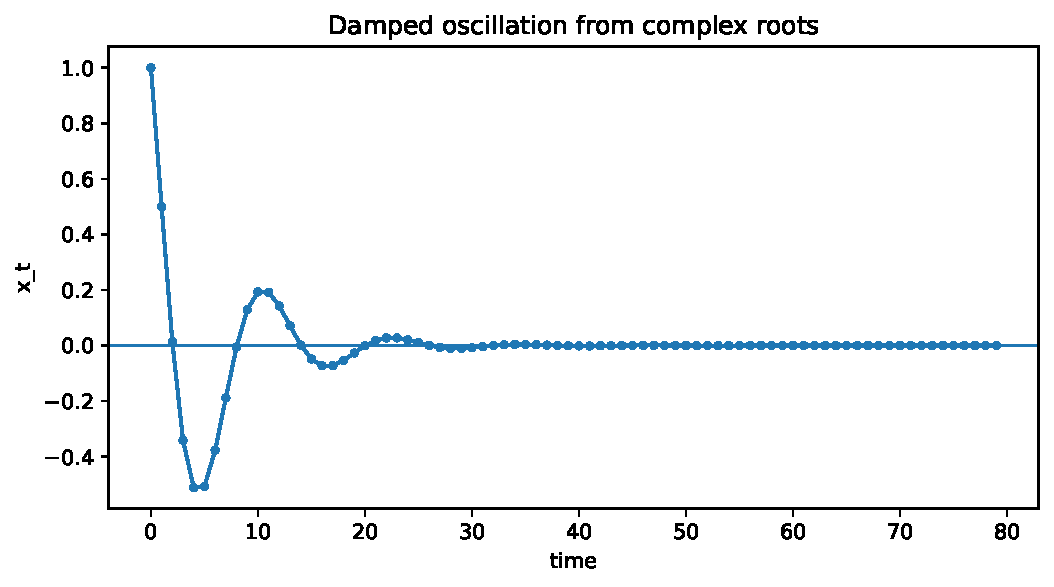
\includegraphics[keepaspectratio]{chapters/chapter-05-difference-equations-dynamic-behavior_files/figure-pdf/py-ch05-damped-recurrence-output-2.pdf}}

The parameter \(r\) controls the damping. Try changing it to \(0.98\)
and then to \(1.02\).

\section{5.16 Python example: impulse response of an
AR(2)}\label{python-example-impulse-response-of-an-ar2}

Now compute the impulse response \(\psi_j\) for

\[
X_t=\phi_1X_{t-1}+\phi_2X_{t-2}+W_t.
\]

The coefficients satisfy

\[
\psi_0=1,
\qquad
\psi_1=\phi_1,
\qquad
\psi_j=\phi_1\psi_{j-1}+\phi_2\psi_{j-2}.
\]

\begin{Shaded}
\begin{Highlighting}[]
\ImportTok{import}\NormalTok{ numpy }\ImportTok{as}\NormalTok{ np}
\ImportTok{import}\NormalTok{ matplotlib.pyplot }\ImportTok{as}\NormalTok{ plt}

\NormalTok{phi1 }\OperatorTok{=} \FloatTok{1.2}
\NormalTok{phi2 }\OperatorTok{=} \OperatorTok{{-}}\FloatTok{0.7}
\NormalTok{horizon }\OperatorTok{=} \DecValTok{50}

\NormalTok{psi }\OperatorTok{=}\NormalTok{ np.zeros(horizon }\OperatorTok{+} \DecValTok{1}\NormalTok{)}
\NormalTok{psi[}\DecValTok{0}\NormalTok{] }\OperatorTok{=} \FloatTok{1.0}
\NormalTok{psi[}\DecValTok{1}\NormalTok{] }\OperatorTok{=}\NormalTok{ phi1}

\ControlFlowTok{for}\NormalTok{ j }\KeywordTok{in} \BuiltInTok{range}\NormalTok{(}\DecValTok{2}\NormalTok{, horizon }\OperatorTok{+} \DecValTok{1}\NormalTok{):}
\NormalTok{    psi[j] }\OperatorTok{=}\NormalTok{ phi1 }\OperatorTok{*}\NormalTok{ psi[j}\OperatorTok{{-}}\DecValTok{1}\NormalTok{] }\OperatorTok{+}\NormalTok{ phi2 }\OperatorTok{*}\NormalTok{ psi[j}\OperatorTok{{-}}\DecValTok{2}\NormalTok{]}

\NormalTok{plt.figure(figsize}\OperatorTok{=}\NormalTok{(}\DecValTok{8}\NormalTok{, }\DecValTok{4}\NormalTok{))}
\NormalTok{plt.stem(}\BuiltInTok{range}\NormalTok{(horizon }\OperatorTok{+} \DecValTok{1}\NormalTok{), psi)}
\NormalTok{plt.axhline(}\DecValTok{0}\NormalTok{, linewidth}\OperatorTok{=}\DecValTok{1}\NormalTok{)}
\NormalTok{plt.xlabel(}\StringTok{"lag j"}\NormalTok{)}
\NormalTok{plt.ylabel(}\StringTok{"psi\_j"}\NormalTok{)}
\NormalTok{plt.title(}\StringTok{"Impulse{-}response coefficients for AR(2)"}\NormalTok{)}
\NormalTok{plt.show()}
\end{Highlighting}
\end{Shaded}

\pandocbounded{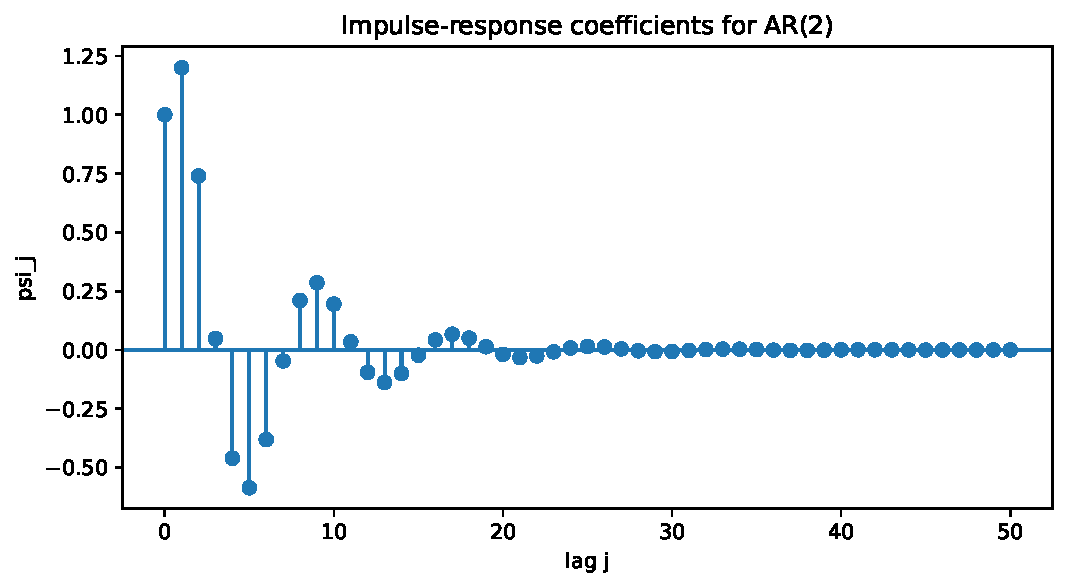
\includegraphics[keepaspectratio]{chapters/chapter-05-difference-equations-dynamic-behavior_files/figure-pdf/py-ch05-impulse-response-output-1.pdf}}

The impulse response is exactly the effect of one unit shock at time
\(t\) on future values \(X_t,X_{t+1},X_{t+2},\ldots\).

\section{5.17 Python example: companion matrix and
eigenvalues}\label{python-example-companion-matrix-and-eigenvalues}

The AR(2) model can be represented by the companion matrix

\[
A=\begin{bmatrix}
\phi_1 & \phi_2\\
1 & 0
\end{bmatrix}.
\]

Its eigenvalues are the forward characteristic roots.

\protect\phantomsection\label{py-ch05-companion-matrix}
\begin{Shaded}
\begin{Highlighting}[]
\ImportTok{import}\NormalTok{ numpy }\ImportTok{as}\NormalTok{ np}

\NormalTok{phi1 }\OperatorTok{=} \FloatTok{1.2}
\NormalTok{phi2 }\OperatorTok{=} \OperatorTok{{-}}\FloatTok{0.7}
\NormalTok{A }\OperatorTok{=}\NormalTok{ np.array([[phi1, phi2],}
\NormalTok{              [}\FloatTok{1.0}\NormalTok{, }\FloatTok{0.0}\NormalTok{]])}

\NormalTok{eigvals }\OperatorTok{=}\NormalTok{ np.linalg.eigvals(A)}
\BuiltInTok{print}\NormalTok{(}\StringTok{"Companion matrix:"}\NormalTok{)}
\BuiltInTok{print}\NormalTok{(A)}
\BuiltInTok{print}\NormalTok{(}\StringTok{"Eigenvalues:"}\NormalTok{, eigvals)}
\BuiltInTok{print}\NormalTok{(}\StringTok{"Spectral radius:"}\NormalTok{, np.}\BuiltInTok{max}\NormalTok{(np.}\BuiltInTok{abs}\NormalTok{(eigvals)))}
\BuiltInTok{print}\NormalTok{(}\StringTok{"Stable forward dynamics?"}\NormalTok{, np.}\BuiltInTok{max}\NormalTok{(np.}\BuiltInTok{abs}\NormalTok{(eigvals)) }\OperatorTok{\textless{}} \DecValTok{1}\NormalTok{)}

\CommentTok{\# Backshift polynomial roots are reciprocals of forward roots.}
\NormalTok{z\_roots }\OperatorTok{=} \DecValTok{1} \OperatorTok{/}\NormalTok{ eigvals}
\BuiltInTok{print}\NormalTok{(}\StringTok{"Backshift roots:"}\NormalTok{, z\_roots)}
\BuiltInTok{print}\NormalTok{(}\StringTok{"Causal AR condition |z| \textgreater{} 1?"}\NormalTok{, np.}\BuiltInTok{all}\NormalTok{(np.}\BuiltInTok{abs}\NormalTok{(z\_roots) }\OperatorTok{\textgreater{}} \DecValTok{1}\NormalTok{))}
\end{Highlighting}
\end{Shaded}

\begin{verbatim}
Companion matrix:
[[ 1.2 -0.7]
 [ 1.   0. ]]
Eigenvalues: [0.6+0.58309519j 0.6-0.58309519j]
Spectral radius: 0.8366600265340757
Stable forward dynamics? True
Backshift roots: [0.85714286-0.83299313j 0.85714286+0.83299313j]
Causal AR condition |z| > 1? True
\end{verbatim}

This example is useful because it connects time-series stability to a
linear algebra concept that students already know: eigenvalues.

\section{5.18 Python example: simulate stable, near-unit, and explosive
AR(1)}\label{python-example-simulate-stable-near-unit-and-explosive-ar1}

A first-order model already shows the three most important regimes.

\begin{Shaded}
\begin{Highlighting}[]
\ImportTok{import}\NormalTok{ numpy }\ImportTok{as}\NormalTok{ np}
\ImportTok{import}\NormalTok{ matplotlib.pyplot }\ImportTok{as}\NormalTok{ plt}

\NormalTok{rng }\OperatorTok{=}\NormalTok{ np.random.default\_rng(}\DecValTok{123}\NormalTok{)}
\NormalTok{n }\OperatorTok{=} \DecValTok{160}
\NormalTok{phis }\OperatorTok{=}\NormalTok{ [}\FloatTok{0.6}\NormalTok{, }\FloatTok{0.98}\NormalTok{, }\FloatTok{1.02}\NormalTok{]}
\NormalTok{labels }\OperatorTok{=}\NormalTok{ [}\StringTok{"stable phi=0.6"}\NormalTok{, }\StringTok{"near unit phi=0.98"}\NormalTok{, }\StringTok{"explosive phi=1.02"}\NormalTok{]}

\NormalTok{plt.figure(figsize}\OperatorTok{=}\NormalTok{(}\DecValTok{9}\NormalTok{, }\DecValTok{5}\NormalTok{))}
\ControlFlowTok{for}\NormalTok{ phi, label }\KeywordTok{in} \BuiltInTok{zip}\NormalTok{(phis, labels):}
\NormalTok{    w }\OperatorTok{=}\NormalTok{ rng.normal(}\DecValTok{0}\NormalTok{, }\DecValTok{1}\NormalTok{, n)}
\NormalTok{    x }\OperatorTok{=}\NormalTok{ np.zeros(n)}
    \ControlFlowTok{for}\NormalTok{ t }\KeywordTok{in} \BuiltInTok{range}\NormalTok{(}\DecValTok{1}\NormalTok{, n):}
\NormalTok{        x[t] }\OperatorTok{=}\NormalTok{ phi }\OperatorTok{*}\NormalTok{ x[t}\OperatorTok{{-}}\DecValTok{1}\NormalTok{] }\OperatorTok{+}\NormalTok{ w[t]}
\NormalTok{    plt.plot(x, label}\OperatorTok{=}\NormalTok{label)}

\NormalTok{plt.axhline(}\DecValTok{0}\NormalTok{, linewidth}\OperatorTok{=}\DecValTok{1}\NormalTok{)}
\NormalTok{plt.xlabel(}\StringTok{"time"}\NormalTok{)}
\NormalTok{plt.ylabel(}\StringTok{"X\_t"}\NormalTok{)}
\NormalTok{plt.title(}\StringTok{"AR(1) dynamic regimes"}\NormalTok{)}
\NormalTok{plt.legend()}
\NormalTok{plt.show()}
\end{Highlighting}
\end{Shaded}

\pandocbounded{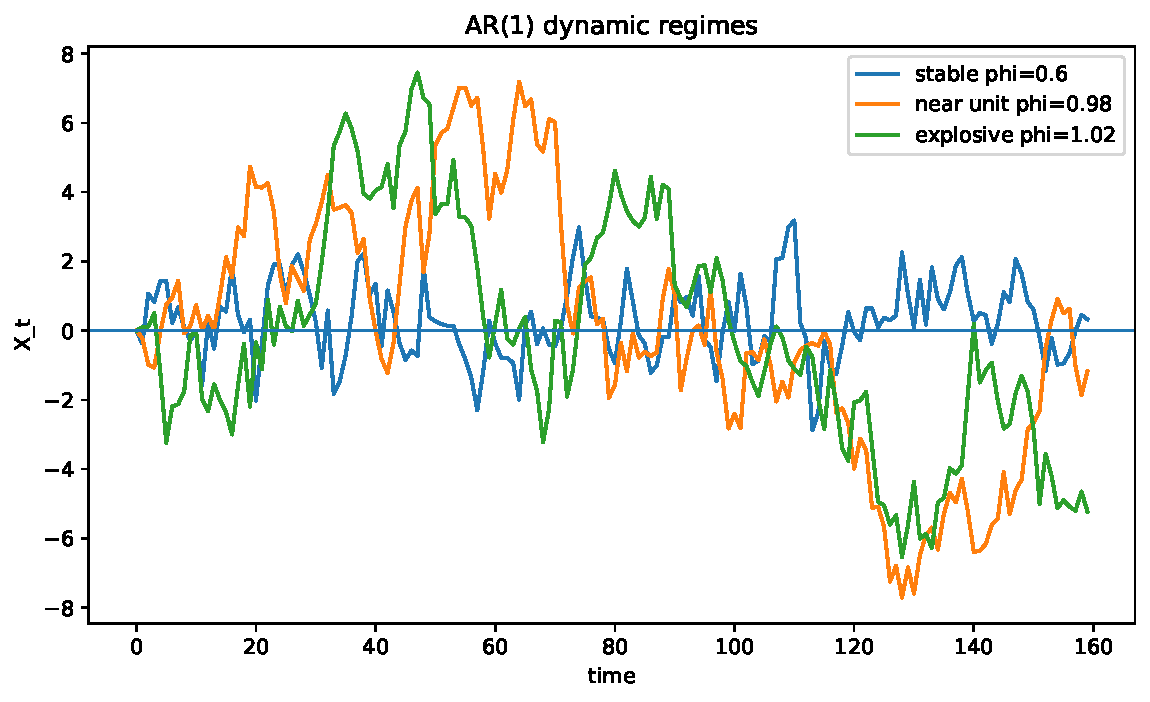
\includegraphics[keepaspectratio]{chapters/chapter-05-difference-equations-dynamic-behavior_files/figure-pdf/py-ch05-ar1-regimes-output-1.pdf}}

Even if \(\phi=1.02\) looks only mildly larger than \(1\), the long-run
behavior changes dramatically.

\section{5.19 AI-assisted study: checking root
conventions}\label{ai-assisted-study-checking-root-conventions}

AI tools are helpful for algebraic manipulation, but root conventions in
time series are a common source of incorrect answers. Use AI as a
checker, not as an authority.

\begin{tcolorbox}[enhanced jigsaw, arc=.35mm, bottomrule=.15mm, bottomtitle=1mm, breakable, colback=white, colbacktitle=quarto-callout-tip-color!10!white, colframe=quarto-callout-tip-color-frame, coltitle=black, left=2mm, leftrule=.75mm, opacityback=0, opacitybacktitle=0.6, rightrule=.15mm, title=\textcolor{quarto-callout-tip-color}{\faLightbulb}\hspace{0.5em}{AI prompt: root convention audit}, titlerule=0mm, toprule=.15mm, toptitle=1mm]

I am studying the AR(2) model \(X_t=\phi_1X_{t-1}+\phi_2X_{t-2}+W_t\).
Explain the difference between roots of the forward characteristic
equation \(\lambda^2-\phi_1\lambda-\phi_2=0\) and roots of the backshift
polynomial \(1-\phi_1z-\phi_2z^2=0\). Verify that \(\lambda=1/z\), and
explain which root condition corresponds to causal stationarity.

\end{tcolorbox}

\begin{tcolorbox}[enhanced jigsaw, arc=.35mm, bottomrule=.15mm, bottomtitle=1mm, breakable, colback=white, colbacktitle=quarto-callout-tip-color!10!white, colframe=quarto-callout-tip-color-frame, coltitle=black, left=2mm, leftrule=.75mm, opacityback=0, opacitybacktitle=0.6, rightrule=.15mm, title=\textcolor{quarto-callout-tip-color}{\faLightbulb}\hspace{0.5em}{AI prompt: recurrence solver}, titlerule=0mm, toprule=.15mm, toptitle=1mm]

Solve the recurrence \(x_t=1.2x_{t-1}-0.7x_{t-2}\) with \(x_0=1\) and
\(x_1=0.5\). First compute the characteristic roots. Then write the
solution in real-valued damped-oscillation form. Finally, give a short
Python snippet that verifies the formula numerically.

\end{tcolorbox}

\begin{tcolorbox}[enhanced jigsaw, arc=.35mm, bottomrule=.15mm, bottomtitle=1mm, breakable, colback=white, colbacktitle=quarto-callout-warning-color!10!white, colframe=quarto-callout-warning-color-frame, coltitle=black, left=2mm, leftrule=.75mm, opacityback=0, opacitybacktitle=0.6, rightrule=.15mm, title=\textcolor{quarto-callout-warning-color}{\faExclamationTriangle}\hspace{0.5em}{What to verify manually}, titlerule=0mm, toprule=.15mm, toptitle=1mm]

When an AI assistant gives an answer, check these four items yourself:

\begin{enumerate}
\def\labelenumi{\arabic{enumi}.}
\tightlist
\item
  Did it use the forward-root or backshift-root convention?
\item
  Did it reverse the stability condition?
\item
  Did it handle complex roots as conjugate pairs?
\item
  Did it confuse deterministic recurrence behavior with stochastic
  stationarity?
\end{enumerate}

\end{tcolorbox}

\section{5.20 Common mistakes}\label{common-mistakes-4}

\subsection{Mistake 1: Saying roots inside the unit circle are always
stable}\label{mistake-1-saying-roots-inside-the-unit-circle-are-always-stable}

This depends on which roots you mean. Forward roots \(\lambda\) must be
inside the unit circle. Backshift roots \(z\) must be outside the unit
circle.

\subsection{Mistake 2: Treating oscillation as
seasonality}\label{mistake-2-treating-oscillation-as-seasonality}

A complex-root AR(2) process can oscillate, but the oscillation is
stochastic and damped. Deterministic seasonality has a more regular
periodic component.

\subsection{Mistake 3: Ignoring roots close to
one}\label{mistake-3-ignoring-roots-close-to-one}

Roots close to the unit circle produce slow decay. A model can be
technically stationary but practically difficult to distinguish from a
nonstationary process in finite samples.

\subsection{Mistake 4: Forgetting initial
conditions}\label{mistake-4-forgetting-initial-conditions}

The constants in the homogeneous solution are determined by initial
conditions. In stochastic stationary modeling, the influence of initial
conditions must decay.

\subsection{Mistake 5: Confusing impulse response and sample
path}\label{mistake-5-confusing-impulse-response-and-sample-path}

The impulse response is deterministic once model parameters are fixed. A
sample path is random because it includes many shocks.

\section{5.21 Mini project: dynamic signatures of AR(2)
models}\label{mini-project-dynamic-signatures-of-ar2-models}

Choose four AR(2) models:

\begin{enumerate}
\def\labelenumi{\arabic{enumi}.}
\tightlist
\item
  two positive real forward roots inside the unit circle;
\item
  one positive and one negative real forward root;
\item
  complex forward roots with radius \(0.75\);
\item
  complex forward roots with radius \(0.98\).
\end{enumerate}

For each model:

\begin{enumerate}
\def\labelenumi{\arabic{enumi}.}
\tightlist
\item
  compute \(\phi_1\) and \(\phi_2\);
\item
  simulate a sample path;
\item
  plot the impulse response;
\item
  plot the sample ACF;
\item
  compute the companion-matrix eigenvalues;
\item
  explain the observed behavior in terms of roots.
\end{enumerate}

Your report should include one paragraph answering:

\begin{quote}
Which model would be hardest to distinguish from a nonstationary process
in a short sample, and why?
\end{quote}

\section{5.22 Exercises}\label{exercises-4}

\subsection{Conceptual exercises}\label{conceptual-exercises-4}

\begin{enumerate}
\def\labelenumi{\arabic{enumi}.}
\tightlist
\item
  Explain why the AR(1) model \(X_t=0.95X_{t-1}+W_t\) is stationary but
  highly persistent.
\item
  Explain why the random walk \(X_t=X_{t-1}+W_t\) is not stationary.
\item
  Give an example of AR(2) forward roots that produce damped oscillation
  with approximate period \(8\).
\item
  Explain the relationship between the roots of
  \(\lambda^2-\phi_1\lambda-\phi_2=0\) and the roots of
  \(1-\phi_1z-\phi_2z^2=0\).
\item
  Why can an AR(2) model have an ACF that oscillates?
\end{enumerate}

\subsection{Mathematical exercises}\label{mathematical-exercises-3}

\begin{enumerate}
\def\labelenumi{\arabic{enumi}.}
\setcounter{enumi}{5}
\tightlist
\item
  Solve the recurrence
\end{enumerate}

\[
x_t=0.7x_{t-1}+0.1x_{t-2}
\]

with \(x_0=1\) and \(x_1=0\).

\begin{enumerate}
\def\labelenumi{\arabic{enumi}.}
\setcounter{enumi}{6}
\item
  Suppose an AR(2) model has forward roots \(0.8\) and \(-0.3\). Find
  \(\phi_1\) and \(\phi_2\).
\item
  Suppose an AR(2) model has forward roots \(0.9e^{\pm i\pi/4}\). Find
  \(\phi_1\) and \(\phi_2\).
\item
  Show that if \(x_t=\phi x_{t-1}\) and \(|\phi|<1\), then \(x_t\to0\).
\item
  Show that the AR(1) autocovariance satisfies
\end{enumerate}

\[
\gamma(h)=\phi\gamma(h-1),
\]

and therefore \(\rho(h)=\phi^h\) for \(h\ge0\).

\subsection{Computational exercises}\label{computational-exercises-2}

\begin{enumerate}
\def\labelenumi{\arabic{enumi}.}
\setcounter{enumi}{10}
\tightlist
\item
  Write a Python function \texttt{ar2\_from\_forward\_roots(r,\ omega)}
  that returns \(\phi_1\) and \(\phi_2\) for complex roots
  \(re^{\pm i\omega}\).
\item
  Write a Python function that computes the first \(m\) impulse-response
  coefficients of an AR(\(p\)) model.
\item
  Simulate AR(2) models with the same root angle but different root
  radii. Compare their sample ACFs.
\item
  Use the companion matrix to check whether the AR(3) model
\end{enumerate}

\[
X_t=0.5X_{t-1}+0.2X_{t-2}-0.1X_{t-3}+W_t
\]

has stable forward dynamics. 15. Generate an explosive AR(1) path with
\(\phi=1.05\). Then difference it and comment on whether the differenced
series appears stationary.

\section{5.23 Chapter checklist}\label{chapter-checklist-2}

By the end of this chapter, you should be able to complete the following
checklist.

\begin{itemize}
\tightlist
\item[$\square$]
  I can write an AR model as a linear difference equation.
\item[$\square$]
  I can solve a first-order homogeneous recurrence.
\item[$\square$]
  I can derive the characteristic equation of an AR(2) recurrence.
\item[$\square$]
  I can explain the difference between forward roots and backshift
  roots.
\item[$\square$]
  I can identify stable, unit-root, and explosive behavior from roots.
\item[$\square$]
  I can explain why complex roots create damped oscillations.
\item[$\square$]
  I can write the repeated-root solution form.
\item[$\square$]
  I can compute AR(2) impulse-response coefficients recursively.
\item[$\square$]
  I can build a companion matrix for an AR(\(p\)) model.
\item[$\square$]
  I can connect eigenvalues of the companion matrix to AR stability.
\item[$\square$]
  I can explain why the ACF of an AR model satisfies a difference
  equation.
\item[$\square$]
  I can use AI to check my algebra without accepting its root convention
  blindly.
\end{itemize}

\section{5.24 Summary}\label{summary}

Difference equations provide the mathematical language for time-series
dynamics. In AR models, the same recurrence controls deterministic
paths, impulse responses, and autocovariance decay. Real roots produce
monotone or alternating decay. Complex roots produce damped
oscillations. Repeated roots create polynomial-exponential behavior. The
companion matrix connects the theory to linear algebra: stability is an
eigenvalue condition.

The next chapter uses these ideas for forecasting. Once we understand
how shocks propagate through a model, we can quantify how uncertainty
grows with the forecast horizon.

\section{Key formulas}\label{key-formulas}

First-order recurrence:

\[
x_t=\phi^t x_0.
\]

AR(2) forward characteristic equation:

\[
\lambda^2-\phi_1\lambda-\phi_2=0.
\]

Backshift polynomial:

\[
\phi(z)=1-\phi_1z-\phi_2z^2.
\]

Root relationship:

\[
\lambda=\frac{1}{z}.
\]

Complex-root AR(2) coefficients:

\[
\lambda_{1,2}=re^{\pm i\omega}
\quad\Longrightarrow\quad
\phi_1=2r\cos(\omega),
\qquad
\phi_2=-r^2.
\]

Damped oscillation solution:

\[
x_t=r^t\{A\cos(\omega t)+B\sin(\omega t)\}.
\]

Repeated-root solution:

\[
x_t=(c_0+c_1t+\cdots+c_{m-1}t^{m-1})\lambda^t.
\]

AR(\(p\)) companion matrix:

\[
A=
\begin{bmatrix}
\phi_1 & \phi_2 & \cdots & \phi_{p-1} & \phi_p\\
1 & 0 & \cdots & 0 & 0\\
0 & 1 & \cdots & 0 & 0\\
\vdots & \vdots & \ddots & \vdots & \vdots\\
0 & 0 & \cdots & 1 & 0
\end{bmatrix}.
\]

Stability in forward-root convention:

\[
\rho(A)<1.
\]

Causal AR condition in backshift-root convention:

\[
\phi(z)=0 \quad\Longrightarrow\quad |z|>1.
\]

\chapter{Forecasting Theory and Best Linear
Prediction}\label{forecasting-theory-and-best-linear-prediction}

\textbf{Part II. Stationarity and Linear Time-Domain Models}\\
\textbf{Chapter goal:} develop forecasting as a mathematical projection
problem. We connect conditional expectation, best linear prediction,
orthogonality of forecast errors, Toeplitz covariance systems, AR and
ARMA forecast recursions, forecast uncertainty, and the practical
workflow used before ARIMA, state-space models, and deep sequence
models.

\section{Learning objectives}\label{learning-objectives-5}

After studying this chapter, you should be able to:

\begin{enumerate}
\def\labelenumi{\arabic{enumi}.}
\tightlist
\item
  define forecasting as prediction of \(X_{n+m}\) from the observed
  history \(X_1,\ldots,X_n\);
\item
  explain why conditional expectation is the minimum mean-square error
  predictor;
\item
  derive the orthogonality equations for best linear prediction;
\item
  write and solve the covariance linear system
  \(\Gamma_n\phi_n=\gamma_n\);
\item
  compute the one-step prediction error variance
  \(\gamma(0)-\gamma_n^T\Gamma_n^{-1}\gamma_n\);
\item
  forecast AR(1), AR(\(p\)), MA(\(q\)), and causal ARMA processes;
\item
  distinguish point forecasts, forecast errors, and forecast intervals;
\item
  understand why recursive forecasting algorithms such as
  Durbin--Levinson, innovations algorithms, and Kalman filters are
  important;
\item
  implement basic forecasting methods in Python without data leakage;
\item
  use AI tools to check derivations and code while preserving the
  mathematical assumptions of time-series forecasting.
\end{enumerate}

\section{6.1 Forecasting as conditional
prediction}\label{forecasting-as-conditional-prediction-1}

Suppose we observe a time series

\[
x_1,x_2,\ldots,x_n.
\]

The forecasting problem is to predict a future value

\[
X_{n+m}, \qquad m\ge 1,
\]

using the information available at time \(n\). The integer \(m\) is
called the \textbf{forecast horizon}. The case \(m=1\) is one-step-ahead
forecasting. The case \(m>1\) is multi-step forecasting.

We write the information available at time \(n\) as

\[
\mathcal F_n=\sigma(X_1,\ldots,X_n),
\]

or, more concretely for this chapter, as the vector

\[
\mathbf X_n=(X_n,X_{n-1},\ldots,X_1)^T.
\]

A forecast is a function of the observed past:

\[
\widehat X_{n+m|n}=g(X_1,\ldots,X_n).
\]

The subscript \(n+m|n\) means: forecast time \(n+m\) using information
through time \(n\).

\begin{tcolorbox}[enhanced jigsaw, arc=.35mm, bottomrule=.15mm, bottomtitle=1mm, breakable, colback=white, colbacktitle=quarto-callout-note-color!10!white, colframe=quarto-callout-note-color-frame, coltitle=black, left=2mm, leftrule=.75mm, opacityback=0, opacitybacktitle=0.6, rightrule=.15mm, title=\textcolor{quarto-callout-note-color}{\faInfo}\hspace{0.5em}{Main idea}, titlerule=0mm, toprule=.15mm, toptitle=1mm]

Forecasting is not guessing the future. Forecasting is choosing a
function of the observed past that minimizes a loss. In classical
time-series theory, the default loss is mean squared error.

\end{tcolorbox}

\section{6.2 The minimum mean-square error
predictor}\label{the-minimum-mean-square-error-predictor}

Let \(Y\) be a random variable we want to predict from information
\(\mathcal F\). We measure prediction quality by mean squared error:

\[
E\left[(Y-g)^2\right],
\]

where \(g\) must be \(\mathcal F\)-measurable. The best predictor among
all measurable functions of the information is the conditional
expectation.

\begin{tcolorbox}[enhanced jigsaw, arc=.35mm, bottomrule=.15mm, bottomtitle=1mm, breakable, colback=white, colbacktitle=quarto-callout-important-color!10!white, colframe=quarto-callout-important-color-frame, coltitle=black, left=2mm, leftrule=.75mm, opacityback=0, opacitybacktitle=0.6, rightrule=.15mm, title=\textcolor{quarto-callout-important-color}{\faExclamation}\hspace{0.5em}{Theorem: conditional expectation is the MMSE predictor}, titlerule=0mm, toprule=.15mm, toptitle=1mm]

Among all predictors \(g\) based on \(\mathcal F\), the unique predictor
minimizing

\[
E\left[(Y-g)^2\right]
\]

is

\[
g^*=E(Y\mid \mathcal F).
\]

\end{tcolorbox}

\subsection{Proof idea}\label{proof-idea}

For any \(\mathcal F\)-measurable \(g\), write

\[
Y-g = \left(Y-E(Y\mid\mathcal F)\right)+\left(E(Y\mid\mathcal F)-g\right).
\]

Squaring and taking expectation gives

\[
E[(Y-g)^2]
=E\left[(Y-E(Y\mid\mathcal F))^2\right]
+E\left[(E(Y\mid\mathcal F)-g)^2\right]
+2E\left[(Y-E(Y\mid\mathcal F))(E(Y\mid\mathcal F)-g)\right].
\]

The cross term is zero because
\(E(Y-E(Y\mid\mathcal F)\mid\mathcal F)=0\). Therefore,

\[
E[(Y-g)^2]
=E\left[(Y-E(Y\mid\mathcal F))^2\right]
+E\left[(E(Y\mid\mathcal F)-g)^2\right].
\]

The second term is nonnegative and is minimized when

\[
g=E(Y\mid\mathcal F).
\]

For forecasting,

\[
\widehat X_{n+m|n}=E(X_{n+m}\mid X_1,\ldots,X_n)
\]

is the optimal mean-square forecast if the conditional expectation is
known.

\begin{tcolorbox}[enhanced jigsaw, arc=.35mm, bottomrule=.15mm, bottomtitle=1mm, breakable, colback=white, colbacktitle=quarto-callout-tip-color!10!white, colframe=quarto-callout-tip-color-frame, coltitle=black, left=2mm, leftrule=.75mm, opacityback=0, opacitybacktitle=0.6, rightrule=.15mm, title=\textcolor{quarto-callout-tip-color}{\faLightbulb}\hspace{0.5em}{Gaussian special case}, titlerule=0mm, toprule=.15mm, toptitle=1mm]

If the time series is Gaussian, conditional expectations are linear
functions of the observed variables. Therefore, for Gaussian time
series, the best linear predictor is also the best predictor among all
measurable predictors.

\end{tcolorbox}

\section{6.3 Why best linear prediction
matters}\label{why-best-linear-prediction-matters}

The conditional expectation may be difficult to compute. It requires
knowledge of the full joint distribution of

\[
(X_1,\ldots,X_n,X_{n+m}).
\]

Classical time-series analysis often restricts attention to
\textbf{linear predictors} because they only require first and second
moments. For a stationary process, those moments are described by the
mean and autocovariance function.

A general linear predictor has the form

\[
\widehat X_{n+m|n}=a_0+a_1X_n+a_2X_{n-1}+\cdots+a_nX_1.
\]

If the process is stationary with mean \(\mu\), it is convenient to
center the variables:

\[
Y_t=X_t-\mu.
\]

Then

\[
\widehat X_{n+m|n}=\mu+\sum_{j=1}^n a_j(X_{n+1-j}-\mu).
\]

Thus, for most derivations, we assume without loss of generality that
\(E(X_t)=0\).

\section{6.4 Orthogonality principle}\label{orthogonality-principle}

For zero-mean data, consider a one-step-ahead linear predictor

\[
\widehat X_{n+1|n}=\phi_{n1}X_n+\phi_{n2}X_{n-1}+\cdots+\phi_{nn}X_1.
\]

Define the prediction error

\[
e_{n+1}=X_{n+1}-\widehat X_{n+1|n}.
\]

The best linear predictor minimizes

\[
E(e_{n+1}^2).
\]

Differentiate the mean squared error with respect to each coefficient
\(\phi_{nk}\). The normal equations are

\[
E\left[e_{n+1}X_{n+1-k}\right]=0,
\qquad k=1,\ldots,n.
\]

Equivalently,

\[
E\left[\left(X_{n+1}-\sum_{j=1}^n\phi_{nj}X_{n+1-j}\right)X_{n+1-k}\right]=0.
\]

\begin{tcolorbox}[enhanced jigsaw, arc=.35mm, bottomrule=.15mm, bottomtitle=1mm, breakable, colback=white, colbacktitle=quarto-callout-note-color!10!white, colframe=quarto-callout-note-color-frame, coltitle=black, left=2mm, leftrule=.75mm, opacityback=0, opacitybacktitle=0.6, rightrule=.15mm, title=\textcolor{quarto-callout-note-color}{\faInfo}\hspace{0.5em}{Orthogonality principle}, titlerule=0mm, toprule=.15mm, toptitle=1mm]

The forecast error of the best linear predictor is orthogonal to every
variable used in the prediction.

This is the same geometric idea as least squares projection: residuals
are orthogonal to the fitted subspace.

\end{tcolorbox}

Using stationarity, the normal equations become

\[
\gamma(k)-\sum_{j=1}^n\phi_{nj}\gamma(k-j)=0,
\qquad k=1,\ldots,n.
\]

Here

\[
\gamma(h)=\operatorname{Cov}(X_{t+h},X_t)
\]

is the autocovariance function.

\section{6.5 Matrix form of the prediction
equations}\label{matrix-form-of-the-prediction-equations}

Define the Toeplitz covariance matrix

\[
\Gamma_n=
\begin{bmatrix}
\gamma(0) & \gamma(1) & \cdots & \gamma(n-1)\\
\gamma(1) & \gamma(0) & \cdots & \gamma(n-2)\\
\vdots & \vdots & \ddots & \vdots\\
\gamma(n-1) & \gamma(n-2) & \cdots & \gamma(0)
\end{bmatrix},
\]

and the covariance vector

\[
\gamma_n=
\begin{bmatrix}
\gamma(1)\\
\gamma(2)\\
\vdots\\
\gamma(n)
\end{bmatrix}.
\]

Let

\[
\phi_n=
\begin{bmatrix}
\phi_{n1}\\
\phi_{n2}\\
\vdots\\
\phi_{nn}
\end{bmatrix}.
\]

Then the prediction equations are

\[
\Gamma_n\phi_n=\gamma_n.
\]

If \(\Gamma_n\) is invertible, then

\[
\phi_n=\Gamma_n^{-1}\gamma_n.
\]

The one-step-ahead forecast is

\[
\widehat X_{n+1|n}=\phi_n^T\mathbf X_n,
\]

where

\[
\mathbf X_n=(X_n,X_{n-1},\ldots,X_1)^T.
\]

\subsection{Prediction error variance}\label{prediction-error-variance}

The mean squared prediction error is

\[
\begin{aligned}
E[(X_{n+1}-\widehat X_{n+1|n})^2]
&=E[(X_{n+1}-\phi_n^T\mathbf X_n)^2]\\
&=\gamma(0)-2\gamma_n^T\phi_n+\phi_n^T\Gamma_n\phi_n.
\end{aligned}
\]

Since \(\Gamma_n\phi_n=\gamma_n\),

\[
E[(X_{n+1}-\widehat X_{n+1|n})^2]
=\gamma(0)-\gamma_n^T\phi_n.
\]

Therefore,

\[
\boxed{\operatorname{MSPE}_n=\gamma(0)-\gamma_n^T\Gamma_n^{-1}\gamma_n.}
\]

\begin{tcolorbox}[enhanced jigsaw, arc=.35mm, bottomrule=.15mm, bottomtitle=1mm, breakable, colback=white, colbacktitle=quarto-callout-important-color!10!white, colframe=quarto-callout-important-color-frame, coltitle=black, left=2mm, leftrule=.75mm, opacityback=0, opacitybacktitle=0.6, rightrule=.15mm, title=\textcolor{quarto-callout-important-color}{\faExclamation}\hspace{0.5em}{Interpretation}, titlerule=0mm, toprule=.15mm, toptitle=1mm]

The term \(\gamma_n^T\Gamma_n^{-1}\gamma_n\) is the reduction in
uncertainty obtained by using the observed past. If the future has
little covariance with the past, this term is small. If the future is
strongly predictable from the past, this term is large.

\end{tcolorbox}

\section{6.6 Interactive: AR(1) forecast
cone}\label{interactive-ar1-forecast-cone}

The AR(1) model is

\[
X_{t+1}=\phi X_t+W_{t+1},
\qquad W_t\sim WN(0,\sigma_w^2).
\]

For \(|\phi|<1\), the \(m\)-step forecast is

\[
\widehat X_{t+m|t}=\phi^mX_t.
\]

The \(m\)-step forecast error variance is

\[
\operatorname{Var}(X_{t+m}-\widehat X_{t+m|t})
=\sigma_w^2\sum_{j=0}^{m-1}\phi^{2j}.
\]

Use the interactive below to see how \(\phi\), the current value
\(X_t\), and the horizon affect the forecast path and uncertainty.

\begin{tcolorbox}[enhanced jigsaw, arc=.35mm, bottomrule=.15mm, bottomtitle=1mm, breakable, colback=white, colbacktitle=quarto-callout-tip-color!10!white, colframe=quarto-callout-tip-color-frame, coltitle=black, left=2mm, leftrule=.75mm, opacityback=0, opacitybacktitle=0.6, rightrule=.15mm, title=\textcolor{quarto-callout-tip-color}{\faLightbulb}\hspace{0.5em}{What to observe}, titlerule=0mm, toprule=.15mm, toptitle=1mm]

When \(|\phi|\) is close to \(1\), the conditional mean decays slowly
and the forecast interval expands slowly toward its long-run variance.
When \(\phi\) is near \(0\), the conditional mean quickly returns to
\(0\) and future uncertainty is dominated by new shocks.

\end{tcolorbox}

\section{6.7 Example: one-step forecast for
AR(1)}\label{example-one-step-forecast-for-ar1}

Assume

\[
X_{t+1}=\phi X_t+W_{t+1},
\qquad E(W_t)=0,
\qquad \operatorname{Var}(W_t)=\sigma_w^2,
\]

with \(|\phi|<1\). The stationary variance is

\[
\gamma(0)=\frac{\sigma_w^2}{1-\phi^2}.
\]

The lag-one covariance is

\[
\gamma(1)=\phi\gamma(0).
\]

For \(n=1\), the best linear predictor of \(X_2\) from \(X_1\) has
coefficient

\[
\phi_{11}=\frac{\gamma(1)}{\gamma(0)}=\phi.
\]

Therefore,

\[
\widehat X_{2|1}=\phi X_1.
\]

The prediction error is

\[
X_2-\widehat X_{2|1}=W_2,
\]

so

\[
\operatorname{MSPE}=\sigma_w^2.
\]

This matches the intuition: for a correctly specified AR(1), the only
unknown part of tomorrow is tomorrow's innovation.

\section{6.8 Multi-step forecasting for
AR(1)}\label{multi-step-forecasting-for-ar1}

For \(m\ge 1\),

\[
X_{t+m}=\phi^mX_t+\phi^{m-1}W_{t+1}+\phi^{m-2}W_{t+2}+\cdots+W_{t+m}.
\]

Taking conditional expectation given \(X_t\) gives

\[
\widehat X_{t+m|t}=\phi^mX_t.
\]

The forecast error is

\[
X_{t+m}-\widehat X_{t+m|t}
=\phi^{m-1}W_{t+1}+\phi^{m-2}W_{t+2}+\cdots+W_{t+m}.
\]

Thus

\[
\operatorname{Var}(X_{t+m}-\widehat X_{t+m|t})
=\sigma_w^2\left(1+\phi^2+\cdots+\phi^{2(m-1)}\right).
\]

If \(|\phi|<1\),

\[
\operatorname{Var}(X_{t+m}-\widehat X_{t+m|t})
=\sigma_w^2\frac{1-\phi^{2m}}{1-\phi^2}.
\]

As \(m\to\infty\),

\[
\widehat X_{t+m|t}\to 0,
\]

and

\[
\operatorname{Var}(X_{t+m}-\widehat X_{t+m|t})\to \frac{\sigma_w^2}{1-\phi^2}=\gamma(0).
\]

Long-horizon forecasts lose memory of the present and approach the
unconditional distribution.

\section{6.9 Forecast intervals}\label{forecast-intervals}

A point forecast is incomplete without uncertainty. If the model is
Gaussian, then

\[
X_{t+m}\mid X_t \sim N\left(\widehat X_{t+m|t},\,\operatorname{Var}(X_{t+m}-\widehat X_{t+m|t})\right).
\]

An approximate 95\% forecast interval is

\[
\widehat X_{t+m|t}
\pm 1.96\sqrt{\operatorname{Var}(X_{t+m}-\widehat X_{t+m|t})}.
\]

\begin{tcolorbox}[enhanced jigsaw, arc=.35mm, bottomrule=.15mm, bottomtitle=1mm, breakable, colback=white, colbacktitle=quarto-callout-warning-color!10!white, colframe=quarto-callout-warning-color-frame, coltitle=black, left=2mm, leftrule=.75mm, opacityback=0, opacitybacktitle=0.6, rightrule=.15mm, title=\textcolor{quarto-callout-warning-color}{\faExclamationTriangle}\hspace{0.5em}{Forecast interval is not a confidence interval for the mean}, titlerule=0mm, toprule=.15mm, toptitle=1mm]

A forecast interval describes uncertainty about a future observation. A
confidence interval describes uncertainty about an estimated parameter
or mean. Forecast intervals are usually wider because they include both
parameter/model uncertainty and future random shocks.

\end{tcolorbox}

\section{6.10 Python example: AR(1) forecast and forecast
intervals}\label{python-example-ar1-forecast-and-forecast-intervals}

\begin{Shaded}
\begin{Highlighting}[]
\ImportTok{import}\NormalTok{ numpy }\ImportTok{as}\NormalTok{ np}
\ImportTok{import}\NormalTok{ pandas }\ImportTok{as}\NormalTok{ pd}
\ImportTok{import}\NormalTok{ matplotlib.pyplot }\ImportTok{as}\NormalTok{ plt}

\NormalTok{rng }\OperatorTok{=}\NormalTok{ np.random.default\_rng(}\DecValTok{7339}\NormalTok{)}

\NormalTok{phi }\OperatorTok{=} \FloatTok{0.75}
\NormalTok{sigma\_w }\OperatorTok{=} \FloatTok{1.0}
\NormalTok{n }\OperatorTok{=} \DecValTok{120}
\NormalTok{x }\OperatorTok{=}\NormalTok{ np.zeros(n)}

\CommentTok{\# Start close to stationarity}
\NormalTok{x[}\DecValTok{0}\NormalTok{] }\OperatorTok{=}\NormalTok{ rng.normal(}\DecValTok{0}\NormalTok{, sigma\_w }\OperatorTok{/}\NormalTok{ np.sqrt(}\DecValTok{1} \OperatorTok{{-}}\NormalTok{ phi}\OperatorTok{**}\DecValTok{2}\NormalTok{))}
\ControlFlowTok{for}\NormalTok{ t }\KeywordTok{in} \BuiltInTok{range}\NormalTok{(}\DecValTok{1}\NormalTok{, n):}
\NormalTok{    x[t] }\OperatorTok{=}\NormalTok{ phi }\OperatorTok{*}\NormalTok{ x[t}\OperatorTok{{-}}\DecValTok{1}\NormalTok{] }\OperatorTok{+}\NormalTok{ rng.normal(}\DecValTok{0}\NormalTok{, sigma\_w)}

\NormalTok{x\_t }\OperatorTok{=}\NormalTok{ x[}\OperatorTok{{-}}\DecValTok{1}\NormalTok{]}
\NormalTok{H }\OperatorTok{=} \DecValTok{25}
\NormalTok{horizons }\OperatorTok{=}\NormalTok{ np.arange(}\DecValTok{1}\NormalTok{, H }\OperatorTok{+} \DecValTok{1}\NormalTok{)}
\NormalTok{forecast\_mean }\OperatorTok{=}\NormalTok{ phi}\OperatorTok{**}\NormalTok{horizons }\OperatorTok{*}\NormalTok{ x\_t}
\NormalTok{forecast\_var }\OperatorTok{=}\NormalTok{ sigma\_w}\OperatorTok{**}\DecValTok{2} \OperatorTok{*}\NormalTok{ np.array([}\BuiltInTok{sum}\NormalTok{(phi}\OperatorTok{**}\NormalTok{(}\DecValTok{2}\OperatorTok{*}\NormalTok{j) }\ControlFlowTok{for}\NormalTok{ j }\KeywordTok{in} \BuiltInTok{range}\NormalTok{(m)) }\ControlFlowTok{for}\NormalTok{ m }\KeywordTok{in}\NormalTok{ horizons])}
\NormalTok{forecast\_se }\OperatorTok{=}\NormalTok{ np.sqrt(forecast\_var)}

\NormalTok{future\_index }\OperatorTok{=}\NormalTok{ np.arange(n, n }\OperatorTok{+}\NormalTok{ H)}

\NormalTok{plt.figure(figsize}\OperatorTok{=}\NormalTok{(}\DecValTok{9}\NormalTok{, }\FloatTok{4.8}\NormalTok{))}
\NormalTok{plt.plot(np.arange(n), x, label}\OperatorTok{=}\StringTok{"observed"}\NormalTok{)}
\NormalTok{plt.plot(future\_index, forecast\_mean, marker}\OperatorTok{=}\StringTok{"o"}\NormalTok{, label}\OperatorTok{=}\StringTok{"forecast mean"}\NormalTok{)}
\NormalTok{plt.fill\_between(}
\NormalTok{    future\_index,}
\NormalTok{    forecast\_mean }\OperatorTok{{-}} \FloatTok{1.96} \OperatorTok{*}\NormalTok{ forecast\_se,}
\NormalTok{    forecast\_mean }\OperatorTok{+} \FloatTok{1.96} \OperatorTok{*}\NormalTok{ forecast\_se,}
\NormalTok{    alpha}\OperatorTok{=}\FloatTok{0.25}\NormalTok{,}
\NormalTok{    label}\OperatorTok{=}\StringTok{"approx. 95}\SpecialCharTok{\% f}\StringTok{orecast interval"}
\NormalTok{)}
\NormalTok{plt.axvline(n }\OperatorTok{{-}} \DecValTok{1}\NormalTok{, linestyle}\OperatorTok{=}\StringTok{"{-}{-}"}\NormalTok{, linewidth}\OperatorTok{=}\DecValTok{1}\NormalTok{)}
\NormalTok{plt.xlabel(}\StringTok{"time"}\NormalTok{)}
\NormalTok{plt.ylabel(}\StringTok{"value"}\NormalTok{)}
\NormalTok{plt.title(}\StringTok{"AR(1) multi{-}step forecast"}\NormalTok{)}
\NormalTok{plt.legend()}
\NormalTok{plt.show()}
\end{Highlighting}
\end{Shaded}

\pandocbounded{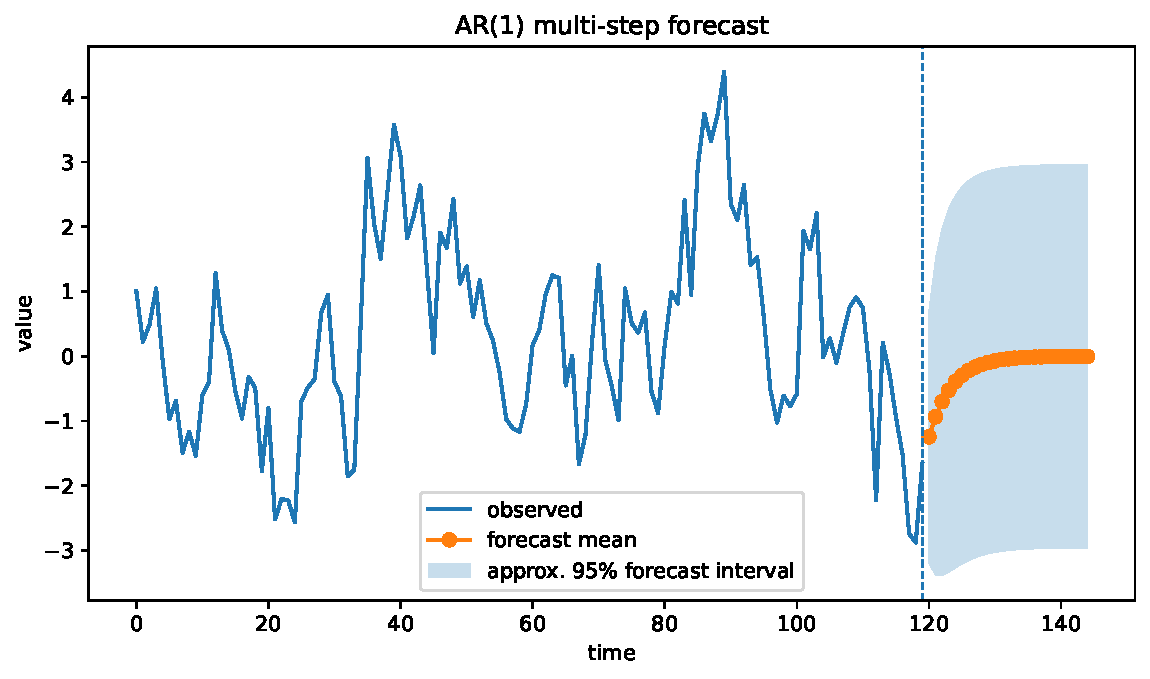
\includegraphics[keepaspectratio]{chapters/chapter-06-forecasting-best-linear-prediction_files/figure-pdf/ch6-python-ar1-forecast-output-1.pdf}}

\section{6.11 Best linear prediction from an autocovariance
function}\label{best-linear-prediction-from-an-autocovariance-function}

The matrix formula

\[
\Gamma_n\phi_n=\gamma_n
\]

is useful because it only needs the autocovariance function. For
example, suppose a process has autocovariance

\[
\gamma(h)=\frac{\sigma_w^2}{1-\phi^2}\phi^{|h|},
\]

which is the autocovariance of a stationary AR(1). If we solve the best
linear prediction equations using many lags, we should discover that
only the first lag is needed.

\begin{Shaded}
\begin{Highlighting}[]
\ImportTok{import}\NormalTok{ numpy }\ImportTok{as}\NormalTok{ np}
\ImportTok{import}\NormalTok{ pandas }\ImportTok{as}\NormalTok{ pd}

\KeywordTok{def}\NormalTok{ ar1\_autocov(phi, sigma\_w, h):}
    \ControlFlowTok{return}\NormalTok{ sigma\_w}\OperatorTok{**}\DecValTok{2} \OperatorTok{/}\NormalTok{ (}\DecValTok{1} \OperatorTok{{-}}\NormalTok{ phi}\OperatorTok{**}\DecValTok{2}\NormalTok{) }\OperatorTok{*}\NormalTok{ phi}\OperatorTok{**}\BuiltInTok{abs}\NormalTok{(h)}

\KeywordTok{def}\NormalTok{ blp\_weights\_from\_autocov(gamma\_func, n\_lags):}
\NormalTok{    Gamma }\OperatorTok{=}\NormalTok{ np.array([}
\NormalTok{        [gamma\_func(i }\OperatorTok{{-}}\NormalTok{ j) }\ControlFlowTok{for}\NormalTok{ j }\KeywordTok{in} \BuiltInTok{range}\NormalTok{(n\_lags)]}
        \ControlFlowTok{for}\NormalTok{ i }\KeywordTok{in} \BuiltInTok{range}\NormalTok{(n\_lags)}
\NormalTok{    ], dtype}\OperatorTok{=}\BuiltInTok{float}\NormalTok{)}
\NormalTok{    gamma\_vec }\OperatorTok{=}\NormalTok{ np.array([gamma\_func(k }\OperatorTok{+} \DecValTok{1}\NormalTok{) }\ControlFlowTok{for}\NormalTok{ k }\KeywordTok{in} \BuiltInTok{range}\NormalTok{(n\_lags)], dtype}\OperatorTok{=}\BuiltInTok{float}\NormalTok{)}
\NormalTok{    weights }\OperatorTok{=}\NormalTok{ np.linalg.solve(Gamma, gamma\_vec)}
\NormalTok{    mspe }\OperatorTok{=}\NormalTok{ gamma\_func(}\DecValTok{0}\NormalTok{) }\OperatorTok{{-}}\NormalTok{ gamma\_vec }\OperatorTok{@}\NormalTok{ weights}
    \ControlFlowTok{return}\NormalTok{ weights, mspe}

\NormalTok{phi\_true }\OperatorTok{=} \FloatTok{0.65}
\NormalTok{sigma\_w }\OperatorTok{=} \FloatTok{1.0}
\NormalTok{weights, mspe }\OperatorTok{=}\NormalTok{ blp\_weights\_from\_autocov(}
    \KeywordTok{lambda}\NormalTok{ h: ar1\_autocov(phi\_true, sigma\_w, h),}
\NormalTok{    n\_lags}\OperatorTok{=}\DecValTok{6}
\NormalTok{)}

\NormalTok{pd.DataFrame(\{}
    \StringTok{"lag"}\NormalTok{: np.arange(}\DecValTok{1}\NormalTok{, }\DecValTok{7}\NormalTok{),}
    \StringTok{"BLP weight"}\NormalTok{: weights}
\NormalTok{\})}
\end{Highlighting}
\end{Shaded}

\protect\phantomsection\label{ch6-python-blp-weights}
{\def\LTcaptype{none} % do not increment counter
\begin{longtable}[]{@{}lll@{}}
\toprule\noalign{}
& lag & BLP weight \\
\midrule\noalign{}
\endhead
\bottomrule\noalign{}
\endlastfoot
0 & 1 & 6.500000e-01 \\
1 & 2 & 3.790162e-16 \\
2 & 3 & -2.513009e-16 \\
3 & 4 & 1.287715e-16 \\
4 & 5 & -7.848340e-17 \\
5 & 6 & 3.852137e-17 \\
\end{longtable}
}

\protect\phantomsection\label{ch6-python-blp-mspe}
\begin{Shaded}
\begin{Highlighting}[]
\BuiltInTok{print}\NormalTok{(}\StringTok{"MSPE from covariance equations:"}\NormalTok{, }\BuiltInTok{round}\NormalTok{(mspe, }\DecValTok{6}\NormalTok{))}
\BuiltInTok{print}\NormalTok{(}\StringTok{"Innovation variance sigma\_w\^{}2:"}\NormalTok{, sigma\_w}\OperatorTok{**}\DecValTok{2}\NormalTok{)}
\end{Highlighting}
\end{Shaded}

\begin{verbatim}
MSPE from covariance equations: 1.0
Innovation variance sigma_w^2: 1.0
\end{verbatim}

The first coefficient is approximately \(\phi\), and the remaining
coefficients are approximately zero. This illustrates the Markov
property of the AR(1) model: after knowing \(X_t\), older observations
do not improve the one-step forecast.

\section{6.12 Interactive: best linear prediction
weights}\label{interactive-best-linear-prediction-weights}

For an AR(1) autocovariance, solve the best linear prediction system
using several past lags. The plot shows the coefficient vector
\(\phi_n\).

\section{\texorpdfstring{6.13 Forecasting AR(\(p\))
models}{6.13 Forecasting AR(p) models}}\label{forecasting-arp-models}

Consider the causal AR(\(p\)) model

\[
X_t=\phi_1X_{t-1}+\phi_2X_{t-2}+\cdots+\phi_pX_{t-p}+W_t.
\]

For one-step-ahead forecasting, if \(t\ge p\), then

\[
\widehat X_{t+1|t}
=\phi_1X_t+\phi_2X_{t-1}+\cdots+\phi_pX_{t-p+1}.
\]

The one-step error is \(W_{t+1}\), so if the parameters are known,

\[
\operatorname{Var}(X_{t+1}-\widehat X_{t+1|t})=\sigma_w^2.
\]

For multi-step forecasting, recursively replace future unknown values by
their forecasts. For example, for AR(2),

\[
X_{t+1}=\phi_1X_t+\phi_2X_{t-1}+W_{t+1},
\]

so

\[
\widehat X_{t+1|t}=\phi_1X_t+\phi_2X_{t-1}.
\]

Then

\[
X_{t+2}=\phi_1X_{t+1}+\phi_2X_t+W_{t+2},
\]

so

\[
\widehat X_{t+2|t}=\phi_1\widehat X_{t+1|t}+\phi_2X_t.
\]

Similarly,

\[
\widehat X_{t+m|t}=\phi_1\widehat X_{t+m-1|t}+\phi_2\widehat X_{t+m-2|t},
\qquad m\ge3.
\]

The rule is simple: use observed values when they are available and
forecasted values when the model refers to future values.

\section{6.14 Companion matrix
representation}\label{companion-matrix-representation-1}

For AR(\(p\)), define the state vector

\[
\mathbf s_t=
\begin{bmatrix}
X_t\\
X_{t-1}\\
\vdots\\
X_{t-p+1}
\end{bmatrix}.
\]

Then

\[
\mathbf s_{t+1}=A\mathbf s_t+\mathbf e_1W_{t+1},
\]

where

\[
A=
\begin{bmatrix}
\phi_1 & \phi_2 & \cdots & \phi_{p-1} & \phi_p\\
1 & 0 & \cdots & 0 & 0\\
0 & 1 & \cdots & 0 & 0\\
\vdots & \vdots & \ddots & \vdots & \vdots\\
0 & 0 & \cdots & 1 & 0
\end{bmatrix}.
\]

The multi-step forecast state is

\[
\widehat{\mathbf s}_{t+m|t}=A^m\mathbf s_t.
\]

The point forecast is the first component:

\[
\widehat X_{t+m|t}=\mathbf e_1^TA^m\mathbf s_t.
\]

This representation makes AR forecasting look like a linear dynamical
system. It also prepares us for state-space models and the Kalman
filter.

\section{6.15 Python example: recursive AR(2)
forecasting}\label{python-example-recursive-ar2-forecasting}

\begin{Shaded}
\begin{Highlighting}[]
\ImportTok{import}\NormalTok{ numpy }\ImportTok{as}\NormalTok{ np}
\ImportTok{import}\NormalTok{ matplotlib.pyplot }\ImportTok{as}\NormalTok{ plt}

\NormalTok{rng }\OperatorTok{=}\NormalTok{ np.random.default\_rng(}\DecValTok{2026}\NormalTok{)}
\NormalTok{phi1, phi2 }\OperatorTok{=} \FloatTok{0.7}\NormalTok{, }\OperatorTok{{-}}\FloatTok{0.25}
\NormalTok{sigma\_w }\OperatorTok{=} \FloatTok{0.8}
\NormalTok{n }\OperatorTok{=} \DecValTok{150}
\NormalTok{x }\OperatorTok{=}\NormalTok{ np.zeros(n)}
\ControlFlowTok{for}\NormalTok{ t }\KeywordTok{in} \BuiltInTok{range}\NormalTok{(}\DecValTok{2}\NormalTok{, n):}
\NormalTok{    x[t] }\OperatorTok{=}\NormalTok{ phi1 }\OperatorTok{*}\NormalTok{ x[t}\OperatorTok{{-}}\DecValTok{1}\NormalTok{] }\OperatorTok{+}\NormalTok{ phi2 }\OperatorTok{*}\NormalTok{ x[t}\OperatorTok{{-}}\DecValTok{2}\NormalTok{] }\OperatorTok{+}\NormalTok{ rng.normal(}\DecValTok{0}\NormalTok{, sigma\_w)}

\NormalTok{H }\OperatorTok{=} \DecValTok{30}
\NormalTok{forecasts }\OperatorTok{=}\NormalTok{ []}
\CommentTok{\# history contains most recent values [X\_t, X\_\{t{-}1\}]}
\NormalTok{history }\OperatorTok{=}\NormalTok{ [x[}\OperatorTok{{-}}\DecValTok{1}\NormalTok{], x[}\OperatorTok{{-}}\DecValTok{2}\NormalTok{]]}

\ControlFlowTok{for}\NormalTok{ m }\KeywordTok{in} \BuiltInTok{range}\NormalTok{(}\DecValTok{1}\NormalTok{, H }\OperatorTok{+} \DecValTok{1}\NormalTok{):}
\NormalTok{    next\_forecast }\OperatorTok{=}\NormalTok{ phi1 }\OperatorTok{*}\NormalTok{ history[}\DecValTok{0}\NormalTok{] }\OperatorTok{+}\NormalTok{ phi2 }\OperatorTok{*}\NormalTok{ history[}\DecValTok{1}\NormalTok{]}
\NormalTok{    forecasts.append(next\_forecast)}
\NormalTok{    history }\OperatorTok{=}\NormalTok{ [next\_forecast, history[}\DecValTok{0}\NormalTok{]]}

\NormalTok{plt.figure(figsize}\OperatorTok{=}\NormalTok{(}\DecValTok{9}\NormalTok{, }\FloatTok{4.8}\NormalTok{))}
\NormalTok{plt.plot(np.arange(n), x, label}\OperatorTok{=}\StringTok{"observed"}\NormalTok{)}
\NormalTok{plt.plot(np.arange(n, n }\OperatorTok{+}\NormalTok{ H), forecasts, marker}\OperatorTok{=}\StringTok{"o"}\NormalTok{, label}\OperatorTok{=}\StringTok{"recursive AR(2) forecast"}\NormalTok{)}
\NormalTok{plt.axvline(n }\OperatorTok{{-}} \DecValTok{1}\NormalTok{, linestyle}\OperatorTok{=}\StringTok{"{-}{-}"}\NormalTok{, linewidth}\OperatorTok{=}\DecValTok{1}\NormalTok{)}
\NormalTok{plt.xlabel(}\StringTok{"time"}\NormalTok{)}
\NormalTok{plt.ylabel(}\StringTok{"value"}\NormalTok{)}
\NormalTok{plt.title(}\StringTok{"Recursive multi{-}step AR(2) forecasting"}\NormalTok{)}
\NormalTok{plt.legend()}
\NormalTok{plt.show()}
\end{Highlighting}
\end{Shaded}

\pandocbounded{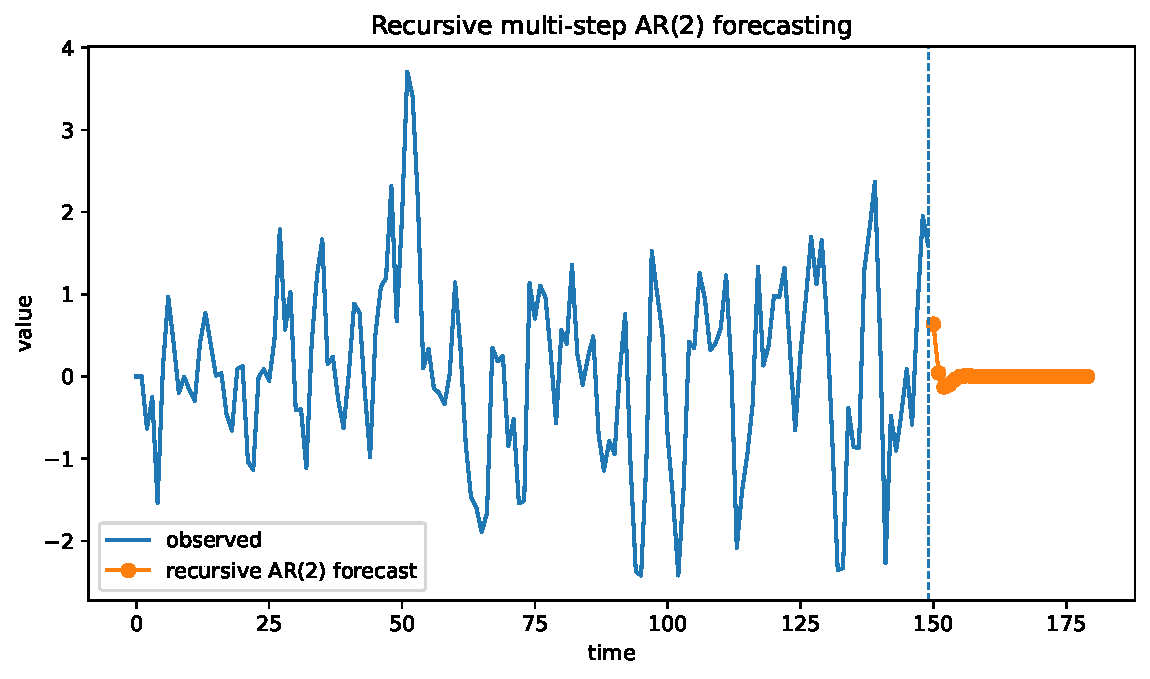
\includegraphics[keepaspectratio]{chapters/chapter-06-forecasting-best-linear-prediction_files/figure-pdf/ch6-python-ar2-recursive-output-1.pdf}}

\section{\texorpdfstring{6.16 MA(\(q\))
forecasting}{6.16 MA(q) forecasting}}\label{maq-forecasting}

Consider an MA(\(q\)) model

\[
X_t=W_t+\theta_1W_{t-1}+\cdots+\theta_qW_{t-q}.
\]

If the innovations \(W_t,W_{t-1},\ldots\) are known, then the one-step
forecast is

\[
\widehat X_{t+1|t}=\theta_1W_t+\theta_2W_{t-1}+\cdots+\theta_qW_{t-q+1}.
\]

The one-step forecast error is \(W_{t+1}\).

For \(m>q\), all innovations appearing in \(X_{t+m}\) are future
innovations, whose conditional expectation is zero. Therefore,

\[
\widehat X_{t+m|t}=0,\qquad m>q,
\]

for a zero-mean MA(\(q\)) process.

\subsection{Important practical issue}\label{important-practical-issue}

In real data, the innovations are not directly observed. They must be
estimated from the fitted model. This is one reason why forecasting ARMA
models requires recursive algorithms.

\section{6.17 Forecasting causal ARMA
processes}\label{forecasting-causal-arma-processes}

A causal ARMA process has the representation

\[
X_t=\psi(B)W_t=\sum_{j=0}^{\infty}\psi_jW_{t-j},
\qquad \psi_0=1.
\]

Then

\[
X_{t+m}=\sum_{j=0}^{m-1}\psi_jW_{t+m-j}
+\sum_{j=m}^{\infty}\psi_jW_{t+m-j}.
\]

The first sum contains future innovations and has conditional
expectation zero. The second sum contains known or estimated past
innovations. Therefore,

\[
\widehat X_{t+m|t}=\sum_{j=m}^{\infty}\psi_jW_{t+m-j}.
\]

The forecast error is

\[
X_{t+m}-\widehat X_{t+m|t}
=\sum_{j=0}^{m-1}\psi_jW_{t+m-j}.
\]

Thus, if \(W_t\) has variance \(\sigma_w^2\),

\[
\operatorname{Var}(X_{t+m}-\widehat X_{t+m|t})
=\sigma_w^2\sum_{j=0}^{m-1}\psi_j^2.
\]

\begin{tcolorbox}[enhanced jigsaw, arc=.35mm, bottomrule=.15mm, bottomtitle=1mm, breakable, colback=white, colbacktitle=quarto-callout-note-color!10!white, colframe=quarto-callout-note-color-frame, coltitle=black, left=2mm, leftrule=.75mm, opacityback=0, opacitybacktitle=0.6, rightrule=.15mm, title=\textcolor{quarto-callout-note-color}{\faInfo}\hspace{0.5em}{Key formula}, titlerule=0mm, toprule=.15mm, toptitle=1mm]

For a causal ARMA model, forecast uncertainty is determined by the
impulse-response weights \(\psi_j\):

\[
\operatorname{MSPE}(m)=\sigma_w^2\sum_{j=0}^{m-1}\psi_j^2.
\]

This formula is one of the cleanest links between ARMA dynamics, shocks,
and forecast uncertainty.

\end{tcolorbox}

\section{6.18 Python example: forecast error variance from impulse
responses}\label{python-example-forecast-error-variance-from-impulse-responses}

\begin{Shaded}
\begin{Highlighting}[]
\ImportTok{import}\NormalTok{ numpy }\ImportTok{as}\NormalTok{ np}
\ImportTok{import}\NormalTok{ pandas }\ImportTok{as}\NormalTok{ pd}

\KeywordTok{def}\NormalTok{ arma\_psi\_weights(ar\_params, ma\_params, max\_lag):}
    \CommentTok{"""}
\CommentTok{    Compute psi weights for an ARMA(p, q) model:}
\CommentTok{    phi(B) X\_t = theta(B) W\_t.}

\CommentTok{    ar\_params = [phi\_1, ..., phi\_p]}
\CommentTok{    ma\_params = [theta\_1, ..., theta\_q]}
\CommentTok{    psi\_0 = 1}
\CommentTok{    """}
\NormalTok{    p }\OperatorTok{=} \BuiltInTok{len}\NormalTok{(ar\_params)}
\NormalTok{    q }\OperatorTok{=} \BuiltInTok{len}\NormalTok{(ma\_params)}
\NormalTok{    psi }\OperatorTok{=}\NormalTok{ np.zeros(max\_lag }\OperatorTok{+} \DecValTok{1}\NormalTok{)}
\NormalTok{    psi[}\DecValTok{0}\NormalTok{] }\OperatorTok{=} \FloatTok{1.0}

    \CommentTok{\# theta\_0 = 1, theta\_j = 0 for j \textgreater{} q}
\NormalTok{    theta }\OperatorTok{=}\NormalTok{ np.zeros(max\_lag }\OperatorTok{+} \DecValTok{1}\NormalTok{)}
\NormalTok{    theta[}\DecValTok{0}\NormalTok{] }\OperatorTok{=} \FloatTok{1.0}
    \ControlFlowTok{for}\NormalTok{ j, val }\KeywordTok{in} \BuiltInTok{enumerate}\NormalTok{(ma\_params, start}\OperatorTok{=}\DecValTok{1}\NormalTok{):}
\NormalTok{        theta[j] }\OperatorTok{=}\NormalTok{ val}

    \ControlFlowTok{for}\NormalTok{ k }\KeywordTok{in} \BuiltInTok{range}\NormalTok{(}\DecValTok{1}\NormalTok{, max\_lag }\OperatorTok{+} \DecValTok{1}\NormalTok{):}
\NormalTok{        ar\_part }\OperatorTok{=} \FloatTok{0.0}
        \ControlFlowTok{for}\NormalTok{ i }\KeywordTok{in} \BuiltInTok{range}\NormalTok{(}\DecValTok{1}\NormalTok{, p }\OperatorTok{+} \DecValTok{1}\NormalTok{):}
            \ControlFlowTok{if}\NormalTok{ k }\OperatorTok{{-}}\NormalTok{ i }\OperatorTok{\textgreater{}=} \DecValTok{0}\NormalTok{:}
\NormalTok{                ar\_part }\OperatorTok{+=}\NormalTok{ ar\_params[i}\OperatorTok{{-}}\DecValTok{1}\NormalTok{] }\OperatorTok{*}\NormalTok{ psi[k}\OperatorTok{{-}}\NormalTok{i]}
\NormalTok{        psi[k] }\OperatorTok{=}\NormalTok{ theta[k] }\OperatorTok{+}\NormalTok{ ar\_part}
    \ControlFlowTok{return}\NormalTok{ psi}

\NormalTok{ar\_params }\OperatorTok{=}\NormalTok{ [}\FloatTok{0.6}\NormalTok{]}
\NormalTok{ma\_params }\OperatorTok{=}\NormalTok{ [}\FloatTok{0.4}\NormalTok{]}
\NormalTok{H }\OperatorTok{=} \DecValTok{12}
\NormalTok{psi }\OperatorTok{=}\NormalTok{ arma\_psi\_weights(ar\_params, ma\_params, max\_lag}\OperatorTok{=}\DecValTok{50}\NormalTok{)}
\NormalTok{sigma\_w }\OperatorTok{=} \FloatTok{1.0}
\NormalTok{mspe }\OperatorTok{=}\NormalTok{ [sigma\_w}\OperatorTok{**}\DecValTok{2} \OperatorTok{*}\NormalTok{ np.}\BuiltInTok{sum}\NormalTok{(psi[:m]}\OperatorTok{**}\DecValTok{2}\NormalTok{) }\ControlFlowTok{for}\NormalTok{ m }\KeywordTok{in} \BuiltInTok{range}\NormalTok{(}\DecValTok{1}\NormalTok{, H }\OperatorTok{+} \DecValTok{1}\NormalTok{)]}

\NormalTok{pd.DataFrame(\{}
    \StringTok{"horizon"}\NormalTok{: np.arange(}\DecValTok{1}\NormalTok{, H }\OperatorTok{+} \DecValTok{1}\NormalTok{),}
    \StringTok{"forecast\_error\_variance"}\NormalTok{: mspe}
\NormalTok{\})}
\end{Highlighting}
\end{Shaded}

\protect\phantomsection\label{ch6-python-psi-forecast-variance}
{\def\LTcaptype{none} % do not increment counter
\begin{longtable}[]{@{}lll@{}}
\toprule\noalign{}
& horizon & forecast\_error\_variance \\
\midrule\noalign{}
\endhead
\bottomrule\noalign{}
\endlastfoot
0 & 1 & 1.000000 \\
1 & 2 & 2.000000 \\
2 & 3 & 2.360000 \\
3 & 4 & 2.489600 \\
4 & 5 & 2.536256 \\
5 & 6 & 2.553052 \\
6 & 7 & 2.559099 \\
7 & 8 & 2.561276 \\
8 & 9 & 2.562059 \\
9 & 10 & 2.562341 \\
10 & 11 & 2.562443 \\
11 & 12 & 2.562479 \\
\end{longtable}
}

\section{6.19 Parameter estimation and
forecasting}\label{parameter-estimation-and-forecasting}

So far, many formulas assumed that the model and its parameters were
known. In practice, we estimate them.

A typical classical workflow is:

\begin{enumerate}
\def\labelenumi{\arabic{enumi}.}
\tightlist
\item
  Plot the time series.
\item
  Transform the data if necessary.
\item
  Remove or difference trend and seasonality if necessary.
\item
  Fit a stationary model to the residual or differenced series.
\item
  Forecast the stationary component.
\item
  Invert transformations to return to the original scale.
\item
  Diagnose forecast errors and residuals.
\end{enumerate}

\subsection{\texorpdfstring{Method of moments for
AR(\(p\))}{Method of moments for AR(p)}}\label{method-of-moments-for-arp}

For a causal AR(\(p\)),

\[
X_t=\phi_1X_{t-1}+\cdots+\phi_pX_{t-p}+W_t.
\]

Multiplying by \(X_{t-h}\) and taking expectations gives the
Yule--Walker equations:

\[
\gamma(h)=\phi_1\gamma(h-1)+\phi_2\gamma(h-2)+\cdots+\phi_p\gamma(h-p),
\qquad h=1,\ldots,p.
\]

In matrix form,

\[
\Gamma_p\phi=\gamma_p.
\]

Replacing population autocovariances by sample autocovariances gives
method-of-moments estimates.

\subsection{Maximum likelihood}\label{maximum-likelihood}

For Gaussian ARMA models, maximum likelihood estimates parameters by
maximizing the likelihood of the observed series. In practice, modern
software usually uses numerical optimization with recursive likelihood
evaluation.

\begin{tcolorbox}[enhanced jigsaw, arc=.35mm, bottomrule=.15mm, bottomtitle=1mm, breakable, colback=white, colbacktitle=quarto-callout-tip-color!10!white, colframe=quarto-callout-tip-color-frame, coltitle=black, left=2mm, leftrule=.75mm, opacityback=0, opacitybacktitle=0.6, rightrule=.15mm, title=\textcolor{quarto-callout-tip-color}{\faLightbulb}\hspace{0.5em}{Theory-to-software connection}, titlerule=0mm, toprule=.15mm, toptitle=1mm]

The same covariance and recursion ideas appear repeatedly: forecasting,
Yule--Walker estimation, innovations algorithms, Kalman filters, and
likelihood evaluation are all versions of the same projection/update
principle.

\end{tcolorbox}

\section{6.20 Python example: rolling one-step forecasts without
leakage}\label{python-example-rolling-one-step-forecasts-without-leakage}

A common mistake is to train on data that includes future observations.
Time-series forecasting must respect chronological order.

\begin{Shaded}
\begin{Highlighting}[]
\ImportTok{import}\NormalTok{ numpy }\ImportTok{as}\NormalTok{ np}
\ImportTok{import}\NormalTok{ matplotlib.pyplot }\ImportTok{as}\NormalTok{ plt}

\NormalTok{rng }\OperatorTok{=}\NormalTok{ np.random.default\_rng(}\DecValTok{11}\NormalTok{)}
\NormalTok{phi }\OperatorTok{=} \FloatTok{0.8}
\NormalTok{sigma\_w }\OperatorTok{=} \FloatTok{1.0}
\NormalTok{n }\OperatorTok{=} \DecValTok{250}
\NormalTok{x }\OperatorTok{=}\NormalTok{ np.zeros(n)}
\ControlFlowTok{for}\NormalTok{ t }\KeywordTok{in} \BuiltInTok{range}\NormalTok{(}\DecValTok{1}\NormalTok{, n):}
\NormalTok{    x[t] }\OperatorTok{=}\NormalTok{ phi }\OperatorTok{*}\NormalTok{ x[t}\OperatorTok{{-}}\DecValTok{1}\NormalTok{] }\OperatorTok{+}\NormalTok{ rng.normal(}\DecValTok{0}\NormalTok{, sigma\_w)}

\NormalTok{train\_size }\OperatorTok{=} \DecValTok{80}
\NormalTok{preds }\OperatorTok{=}\NormalTok{ []}
\NormalTok{actuals }\OperatorTok{=}\NormalTok{ []}
\NormalTok{phis\_hat }\OperatorTok{=}\NormalTok{ []}

\ControlFlowTok{for}\NormalTok{ t }\KeywordTok{in} \BuiltInTok{range}\NormalTok{(train\_size, n }\OperatorTok{{-}} \DecValTok{1}\NormalTok{):}
\NormalTok{    train }\OperatorTok{=}\NormalTok{ x[:t}\OperatorTok{+}\DecValTok{1}\NormalTok{]}
\NormalTok{    y }\OperatorTok{=}\NormalTok{ train[}\DecValTok{1}\NormalTok{:]}
\NormalTok{    z }\OperatorTok{=}\NormalTok{ train[:}\OperatorTok{{-}}\DecValTok{1}\NormalTok{]}
    \CommentTok{\# OLS estimate for AR(1) with zero mean: y\_t = phi z\_t + error\_t}
\NormalTok{    phi\_hat }\OperatorTok{=}\NormalTok{ np.dot(z, y) }\OperatorTok{/}\NormalTok{ np.dot(z, z)}
\NormalTok{    pred }\OperatorTok{=}\NormalTok{ phi\_hat }\OperatorTok{*}\NormalTok{ x[t]}
\NormalTok{    preds.append(pred)}
\NormalTok{    actuals.append(x[t}\OperatorTok{+}\DecValTok{1}\NormalTok{])}
\NormalTok{    phis\_hat.append(phi\_hat)}

\NormalTok{preds }\OperatorTok{=}\NormalTok{ np.array(preds)}
\NormalTok{actuals }\OperatorTok{=}\NormalTok{ np.array(actuals)}
\NormalTok{rmse }\OperatorTok{=}\NormalTok{ np.sqrt(np.mean((actuals }\OperatorTok{{-}}\NormalTok{ preds)}\OperatorTok{**}\DecValTok{2}\NormalTok{))}

\NormalTok{plt.figure(figsize}\OperatorTok{=}\NormalTok{(}\DecValTok{9}\NormalTok{, }\FloatTok{4.8}\NormalTok{))}
\NormalTok{plt.plot(actuals[:}\DecValTok{80}\NormalTok{], label}\OperatorTok{=}\StringTok{"actual next value"}\NormalTok{)}
\NormalTok{plt.plot(preds[:}\DecValTok{80}\NormalTok{], label}\OperatorTok{=}\StringTok{"rolling one{-}step forecast"}\NormalTok{)}
\NormalTok{plt.xlabel(}\StringTok{"forecast origin index"}\NormalTok{)}
\NormalTok{plt.ylabel(}\StringTok{"value"}\NormalTok{)}
\NormalTok{plt.title(}\SpecialStringTok{f"Rolling one{-}step forecasts; RMSE = }\SpecialCharTok{\{}\NormalTok{rmse}\SpecialCharTok{:.3f\}}\SpecialStringTok{"}\NormalTok{)}
\NormalTok{plt.legend()}
\NormalTok{plt.show()}
\end{Highlighting}
\end{Shaded}

\pandocbounded{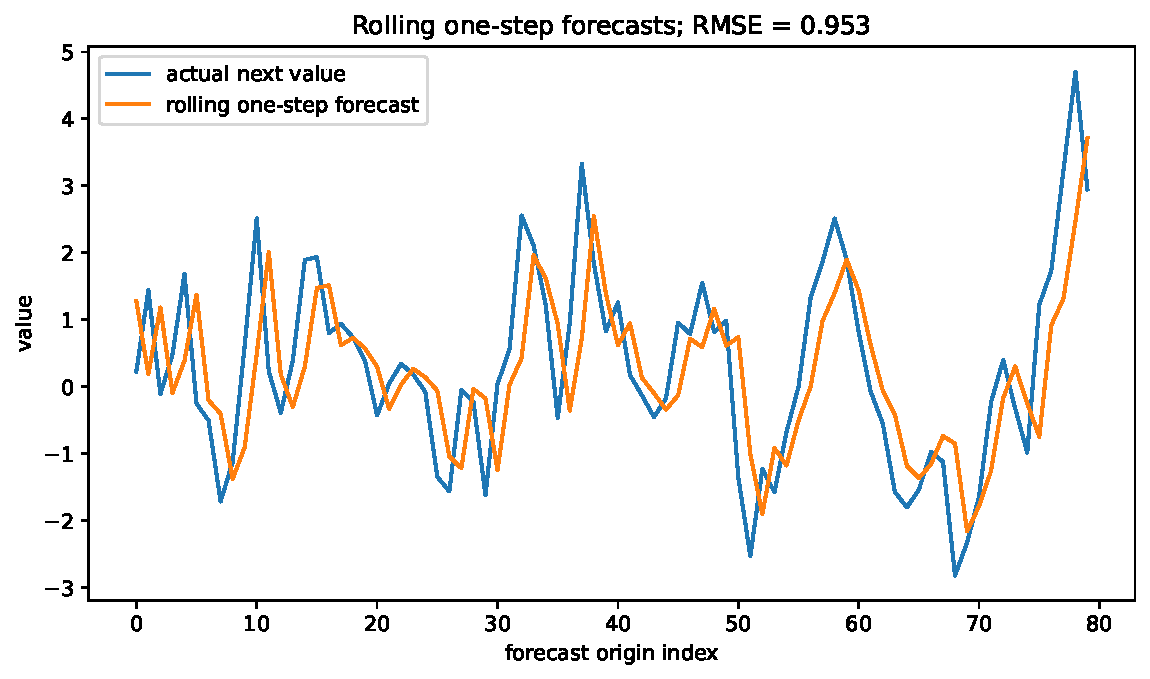
\includegraphics[keepaspectratio]{chapters/chapter-06-forecasting-best-linear-prediction_files/figure-pdf/ch6-python-rolling-forecast-output-1.pdf}}

\section{6.21 Recursive algorithms and bounded
memory}\label{recursive-algorithms-and-bounded-memory}

The covariance equation

\[
\Gamma_n\phi_n=\gamma_n
\]

is conceptually clear, but it has a problem: as \(n\) grows, the system
changes size. Solving a new \(n\times n\) system from scratch at every
time step is expensive.

This motivates recursive forecasting algorithms:

\begin{itemize}
\tightlist
\item
  \textbf{Durbin--Levinson algorithm} solves Toeplitz systems
  efficiently and is central for AR prediction.
\item
  \textbf{Innovations algorithm} updates forecasts using new
  innovations.
\item
  \textbf{Kalman filter} performs recursive prediction and updating for
  state-space models.
\item
  \textbf{Particle filters} extend filtering ideas to nonlinear and
  non-Gaussian state-space models.
\end{itemize}

These algorithms all follow a common pattern:

\[
\text{new forecast} = \text{old forecast} + \text{correction from new information}.
\]

This pattern will return in later chapters when we discuss state-space
models, hidden Markov models, and recurrent neural networks.

\section{6.22 Forecasting after
transformations}\label{forecasting-after-transformations}

Many time series are not stationary on the original scale. Suppose

\[
X_t=\mu_t+Y_t,
\]

where \(\mu_t\) is trend/seasonality and \(Y_t\) is stationary. A common
strategy is:

\begin{enumerate}
\def\labelenumi{\arabic{enumi}.}
\tightlist
\item
  estimate \(\mu_t\);
\item
  compute residuals \(\widehat Y_t=X_t-\widehat\mu_t\);
\item
  forecast \(\widehat Y_{t+m}\) using a stationary model;
\item
  add back the forecasted trend/seasonal component.
\end{enumerate}

If we difference the data, then we must invert differencing after
forecasting. For example, if

\[
Z_t=\nabla X_t=X_t-X_{t-1},
\]

and we forecast \(\widehat Z_{n+1|n},\ldots,\widehat Z_{n+m|n}\), then

\[
\widehat X_{n+m|n}=X_n+\sum_{j=1}^m\widehat Z_{n+j|n}.
\]

\begin{tcolorbox}[enhanced jigsaw, arc=.35mm, bottomrule=.15mm, bottomtitle=1mm, breakable, colback=white, colbacktitle=quarto-callout-warning-color!10!white, colframe=quarto-callout-warning-color-frame, coltitle=black, left=2mm, leftrule=.75mm, opacityback=0, opacitybacktitle=0.6, rightrule=.15mm, title=\textcolor{quarto-callout-warning-color}{\faExclamationTriangle}\hspace{0.5em}{Common mistake}, titlerule=0mm, toprule=.15mm, toptitle=1mm]

Students often forecast differenced data and forget to return to the
original scale. A forecast for \(\nabla X_t\) is not directly a forecast
for \(X_t\).

\end{tcolorbox}

\section{6.23 Forecasting and modern machine
learning}\label{forecasting-and-modern-machine-learning}

The best linear predictor is the classical foundation of forecasting.
Modern machine learning generalizes it in several directions.

{\def\LTcaptype{none} % do not increment counter
\begin{longtable}[]{@{}
  >{\raggedright\arraybackslash}p{(\linewidth - 2\tabcolsep) * \real{0.5000}}
  >{\raggedright\arraybackslash}p{(\linewidth - 2\tabcolsep) * \real{0.5000}}@{}}
\toprule\noalign{}
\begin{minipage}[b]{\linewidth}\raggedright
Classical forecasting object
\end{minipage} & \begin{minipage}[b]{\linewidth}\raggedright
Modern ML analogue
\end{minipage} \\
\midrule\noalign{}
\endhead
\bottomrule\noalign{}
\endlastfoot
\(\widehat X_{t+1|t}=\sum_j a_jX_{t+1-j}\) & linear layer on lag
features \\
AR(\(p\)) & fixed-window autoregressive neural model \\
MA(\(\infty\)) impulse response & convolutional filter over past
shocks/features \\
recursive prediction & recurrent hidden-state update \\
covariance projection & learned representation/projection \\
Gaussian forecast interval & probabilistic neural forecast \\
\end{longtable}
}

A windowed neural network forecast has the form

\[
\widehat X_{t+1|t}=f_\Theta(X_t,X_{t-1},\ldots,X_{t-p+1}),
\]

where \(f_\Theta\) is nonlinear and learned from data. This is a
nonlinear extension of the best linear predictor.

However, the same rule remains: the input window must only use past
information.

\section{6.24 AI-assisted study: useful prompts and
guardrails}\label{ai-assisted-study-useful-prompts-and-guardrails}

AI tools can help you learn forecasting theory, but only if you ask for
verifiable work.

\subsection{Prompt 1: Derivation check}\label{prompt-1-derivation-check}

\begin{quote}
I derived the best linear predictor equations for \(X_{n+1}\) from
\(X_n,\ldots,X_1\). Check whether the orthogonality equations imply
\(\Gamma_n\phi_n=\gamma_n\). Explain every index carefully and identify
possible off-by-one errors.
\end{quote}

\subsection{Prompt 2: Code review for
leakage}\label{prompt-2-code-review-for-leakage}

\begin{quote}
Review this time-series forecasting code. Check whether any future
observations enter the training data, feature construction, scaling, or
validation procedure. Mark every possible source of data leakage.
\end{quote}

\subsection{Prompt 3: Model
interpretation}\label{prompt-3-model-interpretation}

\begin{quote}
I fitted an AR(2) model with coefficients \(\phi_1\) and \(\phi_2\).
Explain how to compute one-step and multi-step forecasts recursively.
Then explain how the characteristic roots affect the shape of the
forecast path.
\end{quote}

\subsection{Prompt 4: Forecast interval
explanation}\label{prompt-4-forecast-interval-explanation}

\begin{quote}
Explain the difference between a confidence interval for a parameter and
a forecast interval for a future observation in an AR(1) model. Use
formulas and a simple numerical example.
\end{quote}

\begin{tcolorbox}[enhanced jigsaw, arc=.35mm, bottomrule=.15mm, bottomtitle=1mm, breakable, colback=white, colbacktitle=quarto-callout-warning-color!10!white, colframe=quarto-callout-warning-color-frame, coltitle=black, left=2mm, leftrule=.75mm, opacityback=0, opacitybacktitle=0.6, rightrule=.15mm, title=\textcolor{quarto-callout-warning-color}{\faExclamationTriangle}\hspace{0.5em}{AI guardrail}, titlerule=0mm, toprule=.15mm, toptitle=1mm]

Do not accept an AI-generated forecast workflow unless it explicitly
states the forecast origin, the training window, the prediction horizon,
and how transformations are inverted. Without those details, the answer
may be mathematically correct but operationally wrong.

\end{tcolorbox}

\section{6.25 Common mistakes}\label{common-mistakes-5}

\begin{enumerate}
\def\labelenumi{\arabic{enumi}.}
\tightlist
\item
  \textbf{Using future data in features.} A rolling mean centered at
  time \(t\) may use future values. Use past-only rolling features for
  forecasting.
\item
  \textbf{Random train-test split.} Random splits destroy time order and
  usually create leakage.
\item
  \textbf{Confusing fitted values with forecasts.} Fitted values use the
  data used to estimate the model. Forecasts predict future unseen
  values.
\item
  \textbf{Ignoring forecast horizon.} A one-step model may perform well
  but fail for long horizons.
\item
  \textbf{Forgetting mean adjustment.} If \(E(X_t)=\mu\), forecast
  deviations from \(\mu\), then add \(\mu\) back.
\item
  \textbf{Forgetting to invert transformations.} Log transforms and
  differencing must be inverted carefully.
\item
  \textbf{Reporting point forecasts only.} Forecast uncertainty is part
  of the model output.
\item
  \textbf{Assuming linear prediction is always optimal.} Linear
  prediction is optimal under Gaussian assumptions, but nonlinear
  dependence may require nonlinear methods.
\end{enumerate}

\section{6.26 Mini project: classical forecasting
report}\label{mini-project-classical-forecasting-report}

Choose one real or simulated time series and produce a short forecasting
report.

\subsection{Requirements}\label{requirements}

\begin{enumerate}
\def\labelenumi{\arabic{enumi}.}
\tightlist
\item
  Plot the series and describe trend, seasonality, outliers, and
  variance changes.
\item
  Choose a stationary transformation or justify why none is needed.
\item
  Fit at least two forecasting models:

  \begin{itemize}
  \tightlist
  \item
    a naive or persistence baseline;
  \item
    an AR or ARMA-type model.
  \end{itemize}
\item
  Use chronological train/test splitting.
\item
  Compare one-step and multi-step forecasts.
\item
  Report RMSE or MAE and include forecast intervals when possible.
\item
  Include a paragraph explaining whether your model uses only past
  information.
\end{enumerate}

\subsection{Suggested datasets}\label{suggested-datasets}

\begin{itemize}
\tightlist
\item
  daily temperature;
\item
  electricity demand;
\item
  S\&P 500 returns;
\item
  airline passengers after log transform;
\item
  simulated AR(2) with complex roots;
\item
  generated seasonal-plus-AR residual data.
\end{itemize}

\section{6.27 Exercises}\label{exercises-5}

\subsection{Conceptual exercises}\label{conceptual-exercises-5}

\begin{enumerate}
\def\labelenumi{\arabic{enumi}.}
\tightlist
\item
  Explain why white noise is difficult to forecast even though its
  distribution is easy to describe.
\item
  What does it mean for a forecast error to be orthogonal to the
  prediction variables?
\item
  Why is conditional expectation the best mean-square predictor?
\item
  Why is the best linear predictor especially important for Gaussian
  time series?
\item
  Explain the difference between \(\widehat X_{t+1|t}\) and
  \(\widehat X_{t+5|t}\).
\item
  Why does forecast uncertainty generally increase with horizon?
\end{enumerate}

\subsection{Mathematical exercises}\label{mathematical-exercises-4}

\begin{enumerate}
\def\labelenumi{\arabic{enumi}.}
\setcounter{enumi}{6}
\tightlist
\item
  Let \(X_t\) be zero-mean stationary with autocovariance \(\gamma(h)\).
  Derive the best linear predictor of \(X_2\) from \(X_1\) and compute
  its MSPE.
\item
  Derive \(\Gamma_2\phi_2=\gamma_2\) explicitly for predicting \(X_3\)
  from \(X_2\) and \(X_1\).
\item
  For AR(1), derive the \(m\)-step forecast and forecast error variance.
\item
  For AR(2), write the recursive formulas for \(\widehat X_{t+1|t}\),
  \(\widehat X_{t+2|t}\), and \(\widehat X_{t+3|t}\).
\item
  For a causal ARMA process \(X_t=\sum_{j=0}^\infty\psi_jW_{t-j}\),
  derive the formula
\end{enumerate}

\[
\operatorname{MSPE}(m)=\sigma_w^2\sum_{j=0}^{m-1}\psi_j^2.
\]

\begin{enumerate}
\def\labelenumi{\arabic{enumi}.}
\setcounter{enumi}{11}
\tightlist
\item
  Suppose \(X_t\) has mean \(\mu\). Derive the centered form of the best
  linear predictor and explain why centering simplifies the equations.
\end{enumerate}

\subsection{Python exercises}\label{python-exercises-2}

\begin{enumerate}
\def\labelenumi{\arabic{enumi}.}
\setcounter{enumi}{12}
\tightlist
\item
  Simulate an AR(1) process with \(\phi=0.9\). Compare one-step rolling
  forecasts with \(\phi\) known and with \(\phi\) estimated recursively.
\item
  Simulate an AR(2) process with complex roots. Plot the forecast path
  from a large positive starting value.
\item
  Implement the covariance matrix \(\Gamma_n\) for a given
  autocovariance function and solve for BLP coefficients.
\item
  Estimate an AR(1) model using only the training set. Forecast the test
  set recursively and compute RMSE.
\item
  Compare random train/test splitting with chronological splitting on a
  simulated AR(1). Explain why the random split is misleading.
\item
  Use bootstrap simulation to estimate empirical forecast intervals for
  an AR(1) and compare them with the Gaussian formula.
\end{enumerate}

\section{6.28 Chapter checklist}\label{chapter-checklist-3}

You are ready to move on when you can:

\begin{itemize}
\tightlist
\item
  state the forecasting problem using \(X_{n+m}\) and \(\mathcal F_n\);
\item
  explain conditional expectation as the MMSE predictor;
\item
  derive the orthogonality equations for best linear prediction;
\item
  write \(\Gamma_n\phi_n=\gamma_n\) and interpret every term;
\item
  compute the MSPE formula;
\item
  forecast AR(1) and AR(\(p\)) models recursively;
\item
  explain why MA and ARMA forecasting depends on innovations;
\item
  compute forecast error variance from \(\psi\) weights;
\item
  construct forecast intervals under Gaussian assumptions;
\item
  evaluate forecasting code for time leakage;
\item
  describe how classical forecasting ideas connect to ML sequence
  models.
\end{itemize}

\section{6.29 Key takeaways}\label{key-takeaways}

Best linear prediction is the mathematical core of classical
forecasting. The forecast is a projection of the future value onto the
space spanned by the observed past. The residual is orthogonal to all
information used in the prediction. For stationary processes, this
projection is determined by the autocovariance function. For AR and ARMA
models, the same theory leads to simple recursive forecasts and explicit
formulas for forecast uncertainty. These ideas remain central in modern
machine learning, where lag windows, convolutional filters, recurrent
states, and attention mechanisms are nonlinear extensions of the same
basic goal: use the past to predict the future without leaking
information from the future.

\chapter{Estimation, Model Identification, and
Diagnostics}\label{estimation-model-identification-and-diagnostics}

\textbf{Part II. Stationarity and Linear Time-Domain Models}\\
\textbf{Chapter goal:} learn how to move from time-series plots and
dependence summaries to fitted models, diagnostic checks, and defensible
model choices. We develop model identification with ACF/PACF, parameter
estimation by moment methods, least squares, and likelihood, residual
diagnostics, information criteria, and AI-assisted model criticism.

\section{Learning objectives}\label{learning-objectives-6}

After studying this chapter, you should be able to:

\begin{enumerate}
\def\labelenumi{\arabic{enumi}.}
\tightlist
\item
  describe the iterative Box--Jenkins modeling workflow: identify,
  estimate, diagnose, revise, forecast;
\item
  use sample ACF and PACF to propose preliminary AR, MA, and ARMA
  orders;
\item
  derive and implement Yule--Walker estimation for AR(\(p\)) models;
\item
  explain conditional least squares and Gaussian maximum likelihood for
  time-series models;
\item
  compare competing models using AIC, AICc, and BIC;
\item
  perform residual diagnostics using time plots, residual ACF,
  Ljung--Box tests, and Q--Q plots;
\item
  recognize underfitting, overfitting, nonstationarity, outliers, and
  changing variance;
\item
  avoid time-series data leakage in estimation, validation, and
  reporting;
\item
  use AI tools to critique a modeling workflow without replacing
  mathematical diagnostics.
\end{enumerate}

\section{7.1 The model-building cycle}\label{the-model-building-cycle}

A fitted time-series model is not finished when software returns
parameter estimates. The main workflow is iterative:

\[
\text{explore} \rightarrow \text{identify} \rightarrow \text{estimate} \rightarrow \text{diagnose} \rightarrow \text{revise} \rightarrow \text{forecast}.
\]

For stationary linear models, the cycle usually begins with a time plot,
ACF, and PACF. These suggest a small collection of candidate models.
After fitting the candidates, we check residuals. If residuals still
contain autocorrelation, trend, seasonality, changing variance, or
outliers, the model has not captured the structure of the data.

\begin{tcolorbox}[enhanced jigsaw, arc=.35mm, bottomrule=.15mm, bottomtitle=1mm, breakable, colback=white, colbacktitle=quarto-callout-note-color!10!white, colframe=quarto-callout-note-color-frame, coltitle=black, left=2mm, leftrule=.75mm, opacityback=0, opacitybacktitle=0.6, rightrule=.15mm, title=\textcolor{quarto-callout-note-color}{\faInfo}\hspace{0.5em}{Principle}, titlerule=0mm, toprule=.15mm, toptitle=1mm]

A good model is not simply a model with low training error. A good
time-series model should leave residuals that look approximately like
white noise and should forecast well on future data.

\end{tcolorbox}

For a parametric model with parameter vector \(\theta\), we write

\[
X_t = m_t(\theta) + e_t(\theta),
\]

where \(m_t(\theta)\) is the model-implied conditional mean and
\(e_t(\theta)\) is the one-step-ahead innovation or residual. A
successful model should make

\[
e_t(\widehat \theta)
\]

approximately uncorrelated, centered, and stable in variance.

\section{7.2 What is being estimated?}\label{what-is-being-estimated}

Consider a zero-mean ARMA(\(p,q\)) model

\[
\phi(B)X_t = \theta(B)W_t,
\]

where

\[
\phi(B)=1-\phi_1B-\cdots-\phi_pB^p,
\]

\[
\theta(B)=1+\theta_1B+\cdots+\theta_qB^q,
\]

and

\[
W_t \sim WN(0,\sigma^2).
\]

The unknown parameter vector is

\[
\vartheta=(\phi_1,\ldots,\phi_p,\theta_1,\ldots,\theta_q,\sigma^2).
\]

If the mean is not zero, we also estimate a mean or intercept term. For
stationary models, mean correction is usually handled by centering the
data or including an intercept.

In practice, we estimate \(\vartheta\) from one realization

\[
x_1,x_2,\ldots,x_n.
\]

This is fundamentally different from ordinary independent-data
regression because neighboring observations are dependent. The
dependence is not a nuisance; it is exactly what we are trying to model.

\section{7.3 Model identification with ACF and
PACF}\label{model-identification-with-acf-and-pacf}

The sample ACF and PACF provide first-order clues about the order of a
linear time-series model.

For stationary data:

{\def\LTcaptype{none} % do not increment counter
\begin{longtable}[]{@{}
  >{\raggedright\arraybackslash}p{(\linewidth - 6\tabcolsep) * \real{0.2500}}
  >{\raggedright\arraybackslash}p{(\linewidth - 6\tabcolsep) * \real{0.2500}}
  >{\raggedright\arraybackslash}p{(\linewidth - 6\tabcolsep) * \real{0.2500}}
  >{\raggedright\arraybackslash}p{(\linewidth - 6\tabcolsep) * \real{0.2500}}@{}}
\toprule\noalign{}
\begin{minipage}[b]{\linewidth}\raggedright
Candidate model
\end{minipage} & \begin{minipage}[b]{\linewidth}\raggedright
ACF pattern
\end{minipage} & \begin{minipage}[b]{\linewidth}\raggedright
PACF pattern
\end{minipage} & \begin{minipage}[b]{\linewidth}\raggedright
Interpretation
\end{minipage} \\
\midrule\noalign{}
\endhead
\bottomrule\noalign{}
\endlastfoot
AR(\(p\)) & tails off gradually & cuts off after lag \(p\) & finite
memory in regression on past values \\
MA(\(q\)) & cuts off after lag \(q\) & tails off gradually & finite
memory in shocks \\
ARMA(\(p,q\)) & tails off gradually & tails off gradually & mixed
dependence structure \\
White noise & insignificant after lag 0 & insignificant after lag 0 & no
useful linear dependence \\
Nonstationary trend & slow decay & often slow decay & difference or
detrend first \\
\end{longtable}
}

Here ``cuts off'' means the theoretical quantity is exactly zero beyond
a finite lag. In finite samples, sample estimates rarely equal exactly
zero, so we look for values inside approximate confidence bands.

For white noise, the sample autocorrelations are approximately

\[
\widehat \rho(h) \approx N\left(0,\frac{1}{n}\right),
\]

so a rough \(95\%\) band is

\[
\pm \frac{1.96}{\sqrt n}.
\]

\begin{tcolorbox}[enhanced jigsaw, arc=.35mm, bottomrule=.15mm, bottomtitle=1mm, breakable, colback=white, colbacktitle=quarto-callout-warning-color!10!white, colframe=quarto-callout-warning-color-frame, coltitle=black, left=2mm, leftrule=.75mm, opacityback=0, opacitybacktitle=0.6, rightrule=.15mm, title=\textcolor{quarto-callout-warning-color}{\faExclamationTriangle}\hspace{0.5em}{Do not overread the ACF}, titlerule=0mm, toprule=.15mm, toptitle=1mm]

The ACF and PACF are screening tools, not final proof. A few significant
lags may occur by chance, and nonstationarity can create misleading slow
decay. Always check residuals after fitting.

\end{tcolorbox}

\subsection{ACF and PACF logic}\label{acf-and-pacf-logic}

For an AR(\(p\)) model,

\[
X_t=\phi_1X_{t-1}+\cdots+\phi_pX_{t-p}+W_t,
\]

the best linear predictor using the infinite past only needs the most
recent \(p\) values. Therefore, the partial autocorrelation becomes zero
beyond lag \(p\).

For an MA(\(q\)) model,

\[
X_t=W_t+\theta_1W_{t-1}+\cdots+\theta_qW_{t-q},
\]

\(X_t\) and \(X_{t-h}\) share no common shocks when \(h>q\). Therefore,

\[
\rho(h)=0, \qquad h>q.
\]

This is why the ACF identifies MA order more directly and the PACF
identifies AR order more directly.

\section{7.4 Sample autocovariance and sample
ACF}\label{sample-autocovariance-and-sample-acf}

Given observations \(x_1,\ldots,x_n\), define the sample mean

\[
\bar x=\frac{1}{n}\sum_{t=1}^n x_t.
\]

A common estimator of the autocovariance is

\[
\widehat\gamma(h)
=\frac{1}{n}\sum_{t=1}^{n-h}(x_{t+h}-\bar x)(x_t-\bar x),
\qquad h=0,1,\ldots,n-1.
\]

The sample autocorrelation is

\[
\widehat\rho(h)=\frac{\widehat\gamma(h)}{\widehat\gamma(0)}.
\]

The denominator uses \(\widehat\gamma(0)\), the sample variance computed
with divisor \(n\). Some software uses slightly different conventions.
These differences matter less than the modeling interpretation.

\begin{tcolorbox}[enhanced jigsaw, arc=.35mm, bottomrule=.15mm, bottomtitle=1mm, breakable, colback=white, colbacktitle=quarto-callout-tip-color!10!white, colframe=quarto-callout-tip-color-frame, coltitle=black, left=2mm, leftrule=.75mm, opacityback=0, opacitybacktitle=0.6, rightrule=.15mm, title=\textcolor{quarto-callout-tip-color}{\faLightbulb}\hspace{0.5em}{Estimator convention}, titlerule=0mm, toprule=.15mm, toptitle=1mm]

Using divisor \(n\) produces a positive semidefinite sample
autocovariance sequence, which is useful when forming Toeplitz
covariance matrices.

\end{tcolorbox}

\section{\texorpdfstring{7.5 Yule--Walker estimation for
AR(\(p\))}{7.5 Yule--Walker estimation for AR(p)}}\label{yulewalker-estimation-for-arp}

For a stationary AR(\(p\)) process,

\[
X_t=\phi_1X_{t-1}+\cdots+\phi_pX_{t-p}+W_t,
\]

multiply both sides by \(X_{t-h}\) and take expectations. For
\(h=1,\ldots,p\),

\[
\gamma(h)=\phi_1\gamma(h-1)+\phi_2\gamma(h-2)+\cdots+\phi_p\gamma(h-p).
\]

In matrix form,

\[
\begin{bmatrix}
\gamma(0) & \gamma(1) & \cdots & \gamma(p-1) \\
\gamma(1) & \gamma(0) & \cdots & \gamma(p-2) \\
\vdots & \vdots & \ddots & \vdots \\
\gamma(p-1) & \gamma(p-2) & \cdots & \gamma(0)
\end{bmatrix}
\begin{bmatrix}
\phi_1 \\
\phi_2 \\
\vdots \\
\phi_p
\end{bmatrix}
=
\begin{bmatrix}
\gamma(1) \\
\gamma(2) \\
\vdots \\
\gamma(p)
\end{bmatrix}.
\]

Replacing \(\gamma(h)\) by \(\widehat\gamma(h)\) gives the Yule--Walker
estimator:

\[
\widehat{\boldsymbol\phi}_{YW}=\widehat\Gamma_p^{-1}\widehat{\boldsymbol\gamma}_p.
\]

The innovation variance is estimated by

\[
\widehat\sigma^2
=\widehat\gamma(0)-\widehat{\boldsymbol\gamma}_p^T\widehat\Gamma_p^{-1}\widehat{\boldsymbol\gamma}_p.
\]

\subsection{Why Yule--Walker is useful}\label{why-yulewalker-is-useful}

Yule--Walker estimation is fast, interpretable, and closely connected to
best linear prediction. It is especially useful for AR models and for
initializing more complicated likelihood-based algorithms.

\subsection{Why Yule--Walker is
limited}\label{why-yulewalker-is-limited}

Yule--Walker is designed for AR models. For ARMA models, the
moving-average part introduces latent innovations \(W_t\) that are not
directly observed. In that case, likelihood or nonlinear least squares
methods are usually preferred.

\section{7.6 Conditional least squares}\label{conditional-least-squares}

For an AR(\(p\)) model, conditional least squares is ordinary least
squares applied to the regression

\[
X_t=\phi_1X_{t-1}+\cdots+\phi_pX_{t-p}+W_t,
\qquad t=p+1,\ldots,n.
\]

Define

\[
\mathbf y=
\begin{bmatrix}
x_{p+1} \\
x_{p+2} \\
\vdots \\
x_n
\end{bmatrix},
\qquad
Z=
\begin{bmatrix}
x_p & x_{p-1} & \cdots & x_1 \\
x_{p+1} & x_p & \cdots & x_2 \\
\vdots & \vdots & \ddots & \vdots \\
x_{n-1} & x_{n-2} & \cdots & x_{n-p}
\end{bmatrix}.
\]

Then

\[
\widehat{\boldsymbol\phi}_{CLS}=(Z^TZ)^{-1}Z^T\mathbf y.
\]

This is simple because AR residuals can be computed directly:

\[
e_t(\phi)=x_t-\phi_1x_{t-1}-\cdots-\phi_px_{t-p}.
\]

For ARMA models, residuals depend recursively on previous residuals:

\[
e_t(\vartheta)=x_t-\phi_1x_{t-1}-\cdots-\phi_px_{t-p}
-\theta_1e_{t-1}(\vartheta)-\cdots-\theta_qe_{t-q}(\vartheta).
\]

The conditional sum of squares is

\[
S(\vartheta)=\sum_{t=m+1}^n e_t(\vartheta)^2,
\]

where \(m=\max(p,q)\) and initial residuals are handled by convention.
The estimator minimizes \(S(\vartheta)\) subject to stationarity and
invertibility restrictions.

\begin{tcolorbox}[enhanced jigsaw, arc=.35mm, bottomrule=.15mm, bottomtitle=1mm, breakable, colback=white, colbacktitle=quarto-callout-note-color!10!white, colframe=quarto-callout-note-color-frame, coltitle=black, left=2mm, leftrule=.75mm, opacityback=0, opacitybacktitle=0.6, rightrule=.15mm, title=\textcolor{quarto-callout-note-color}{\faInfo}\hspace{0.5em}{Computational point}, titlerule=0mm, toprule=.15mm, toptitle=1mm]

For AR models, conditional least squares is linear least squares. For
ARMA models, conditional least squares is nonlinear because residuals
depend recursively on the MA parameters.

\end{tcolorbox}

\section{7.7 Gaussian maximum
likelihood}\label{gaussian-maximum-likelihood}

If the innovations are Gaussian,

\[
W_t \sim N(0,\sigma^2),
\]

then the vector

\[
\mathbf X=(X_1,\ldots,X_n)^T
\]

is multivariate normal for a stationary Gaussian model:

\[
\mathbf X\sim N(\boldsymbol\mu,\Sigma_\vartheta).
\]

The log-likelihood is

\[
\ell(\vartheta)
=-\frac{n}{2}\log(2\pi)
-\frac{1}{2}\log |\Sigma_\vartheta|
-\frac{1}{2}(\mathbf x-\boldsymbol\mu)^T\Sigma_\vartheta^{-1}(\mathbf x-\boldsymbol\mu).
\]

Maximum likelihood estimation chooses

\[
\widehat\vartheta_{MLE}=\arg\max_\vartheta \ell(\vartheta).
\]

Exact likelihood accounts for the full joint distribution of the
observed vector. Conditional likelihood approximates the likelihood by
conditioning on initial observations or initial residuals.

For many ARMA and ARIMA models, software uses state-space or innovations
algorithms to compute the likelihood efficiently without explicitly
inverting a large \(n\times n\) covariance matrix.

\begin{tcolorbox}[enhanced jigsaw, arc=.35mm, bottomrule=.15mm, bottomtitle=1mm, breakable, colback=white, colbacktitle=quarto-callout-important-color!10!white, colframe=quarto-callout-important-color-frame, coltitle=black, left=2mm, leftrule=.75mm, opacityback=0, opacitybacktitle=0.6, rightrule=.15mm, title=\textcolor{quarto-callout-important-color}{\faExclamation}\hspace{0.5em}{Why likelihood matters}, titlerule=0mm, toprule=.15mm, toptitle=1mm]

Maximum likelihood gives a unified framework for estimation, standard
errors, model comparison, missing-data handling, and forecast
uncertainty. But it still depends on model assumptions.

\end{tcolorbox}

\section{7.8 Standard errors and coefficient
significance}\label{standard-errors-and-coefficient-significance}

After fitting a parametric model, software often reports standard errors
for estimated coefficients. A common approximate statistic is

\[
z_j=\frac{\widehat\vartheta_j}{\operatorname{se}(\widehat\vartheta_j)}.
\]

Large values of \(|z_j|\) suggest that the parameter is distinguishable
from zero under the fitted model.

However, coefficient significance should not be used mechanically. A
parameter can be statistically significant but practically irrelevant,
and a nonsignificant parameter may appear because the model is
overparameterized or the sample is short.

\begin{tcolorbox}[enhanced jigsaw, arc=.35mm, bottomrule=.15mm, bottomtitle=1mm, breakable, colback=white, colbacktitle=quarto-callout-warning-color!10!white, colframe=quarto-callout-warning-color-frame, coltitle=black, left=2mm, leftrule=.75mm, opacityback=0, opacitybacktitle=0.6, rightrule=.15mm, title=\textcolor{quarto-callout-warning-color}{\faExclamationTriangle}\hspace{0.5em}{Parameter significance is not model adequacy}, titlerule=0mm, toprule=.15mm, toptitle=1mm]

A model with significant coefficients can still have autocorrelated
residuals, wrong variance structure, or poor forecasts. Residual
diagnostics are essential.

\end{tcolorbox}

\section{7.9 Information criteria: AIC, AICc, and
BIC}\label{information-criteria-aic-aicc-and-bic}

Suppose a fitted model has maximized log-likelihood
\(\ell(\widehat\vartheta)\) and \(k\) estimated parameters. The Akaike
information criterion is

\[
AIC=-2\ell(\widehat\vartheta)+2k.
\]

A finite-sample corrected version is

\[
AICc=AIC+\frac{2k(k+1)}{n-k-1}.
\]

The Bayesian information criterion is

\[
BIC=-2\ell(\widehat\vartheta)+k\log n.
\]

Lower values are preferred among models fit to the same data with
comparable likelihoods.

\subsection{Interpretation}\label{interpretation-3}

AIC tends to choose models with better predictive flexibility. BIC
penalizes complexity more strongly and tends to choose simpler models as
\(n\) grows.

\begin{tcolorbox}[enhanced jigsaw, arc=.35mm, bottomrule=.15mm, bottomtitle=1mm, breakable, colback=white, colbacktitle=quarto-callout-tip-color!10!white, colframe=quarto-callout-tip-color-frame, coltitle=black, left=2mm, leftrule=.75mm, opacityback=0, opacitybacktitle=0.6, rightrule=.15mm, title=\textcolor{quarto-callout-tip-color}{\faLightbulb}\hspace{0.5em}{Use information criteria as filters}, titlerule=0mm, toprule=.15mm, toptitle=1mm]

Information criteria help compare candidate models. They do not replace
residual diagnostics, forecast backtesting, or scientific
interpretation.

\end{tcolorbox}

\section{7.10 Residual diagnostics}\label{residual-diagnostics}

Let \(\widehat e_t\) be the residuals from a fitted model. Diagnostics
ask whether \(\widehat e_t\) behaves like white noise.

A useful diagnostic set includes:

\begin{enumerate}
\def\labelenumi{\arabic{enumi}.}
\tightlist
\item
  residual time plot;
\item
  histogram and Q--Q plot;
\item
  residual ACF and PACF;
\item
  Ljung--Box test;
\item
  residuals versus fitted values;
\item
  squared residual ACF for changing variance.
\end{enumerate}

\subsection{Residual time plot}\label{residual-time-plot}

The residual time plot should show no obvious trend, seasonal pattern,
level shift, or changing variance. Outliers should be investigated.

\subsection{Residual ACF}\label{residual-acf}

The residual ACF should have most nonzero-lag values inside the
approximate band

\[
\pm \frac{1.96}{\sqrt n}.
\]

A large residual autocorrelation at lag \(h\) suggests that the fitted
model did not explain dependence at that lag.

\subsection{Q--Q plot}\label{qq-plot}

A Q--Q plot compares residual quantiles with normal quantiles. Strong
curvature, heavy tails, or extreme points suggest non-Gaussian
residuals. For point forecasting, mild nonnormality may be acceptable;
for interval forecasting, it matters more.

\section{7.11 Ljung--Box test}\label{ljungbox-test}

The Ljung--Box statistic tests whether a collection of residual
autocorrelations is jointly small. For maximum lag \(H\),

\[
Q(H)=n(n+2)\sum_{h=1}^H \frac{\widehat\rho_e(h)^2}{n-h},
\]

where \(\widehat\rho_e(h)\) is the residual sample autocorrelation at
lag \(h\).

Under the null hypothesis that residuals are white noise, approximately

\[
Q(H)\sim \chi^2_{H-k},
\]

where \(k\) is often taken as the number of fitted ARMA parameters. A
small \(p\)-value suggests remaining autocorrelation.

\begin{tcolorbox}[enhanced jigsaw, arc=.35mm, bottomrule=.15mm, bottomtitle=1mm, breakable, colback=white, colbacktitle=quarto-callout-warning-color!10!white, colframe=quarto-callout-warning-color-frame, coltitle=black, left=2mm, leftrule=.75mm, opacityback=0, opacitybacktitle=0.6, rightrule=.15mm, title=\textcolor{quarto-callout-warning-color}{\faExclamationTriangle}\hspace{0.5em}{Practical caution}, titlerule=0mm, toprule=.15mm, toptitle=1mm]

The Ljung--Box test is sensitive to the choice of \(H\), sample size,
and estimated parameters. Use it together with residual plots, not by
itself.

\end{tcolorbox}

\section{7.12 Interactive HTML: model identification
simulator}\label{interactive-html-model-identification-simulator}

This interactive module simulates an ARMA(1,1) model

\[
X_t=\phi X_{t-1}+W_t+\theta W_{t-1}
\]

and displays the time plot, sample ACF, and sample PACF. The goal is to
help you see why AR, MA, and ARMA models produce different empirical
signatures.

\begin{tcolorbox}[enhanced jigsaw, arc=.35mm, bottomrule=.15mm, bottomtitle=1mm, breakable, colback=white, colbacktitle=quarto-callout-note-color!10!white, colframe=quarto-callout-note-color-frame, coltitle=black, left=2mm, leftrule=.75mm, opacityback=0, opacitybacktitle=0.6, rightrule=.15mm, title=\textcolor{quarto-callout-note-color}{\faInfo}\hspace{0.5em}{Note}, titlerule=0mm, toprule=.15mm, toptitle=1mm]

The simulator relies on Plotly being loaded globally through the book
header. Do not add a second Plotly script tag inside this chapter.

\end{tcolorbox}

\section{7.13 Python example: ACF, PACF, and Yule--Walker from
scratch}\label{python-example-acf-pacf-and-yulewalker-from-scratch}

The following example simulates an AR(2) process and estimates its
coefficients by Yule--Walker.

\protect\phantomsection\label{py-ch07-yule-walker}
\begin{Shaded}
\begin{Highlighting}[]
\ImportTok{import}\NormalTok{ numpy }\ImportTok{as}\NormalTok{ np}
\ImportTok{import}\NormalTok{ matplotlib.pyplot }\ImportTok{as}\NormalTok{ plt}

\NormalTok{np.random.seed(}\DecValTok{7339}\NormalTok{)}

\NormalTok{n }\OperatorTok{=} \DecValTok{600}
\NormalTok{burn }\OperatorTok{=} \DecValTok{200}
\NormalTok{phi\_true }\OperatorTok{=}\NormalTok{ np.array([}\FloatTok{0.65}\NormalTok{, }\OperatorTok{{-}}\FloatTok{0.30}\NormalTok{])}
\NormalTok{w }\OperatorTok{=}\NormalTok{ np.random.normal(size}\OperatorTok{=}\NormalTok{n }\OperatorTok{+}\NormalTok{ burn)}
\NormalTok{x }\OperatorTok{=}\NormalTok{ np.zeros(n }\OperatorTok{+}\NormalTok{ burn)}

\ControlFlowTok{for}\NormalTok{ t }\KeywordTok{in} \BuiltInTok{range}\NormalTok{(}\DecValTok{2}\NormalTok{, n }\OperatorTok{+}\NormalTok{ burn):}
\NormalTok{    x[t] }\OperatorTok{=}\NormalTok{ phi\_true[}\DecValTok{0}\NormalTok{] }\OperatorTok{*}\NormalTok{ x[t}\OperatorTok{{-}}\DecValTok{1}\NormalTok{] }\OperatorTok{+}\NormalTok{ phi\_true[}\DecValTok{1}\NormalTok{] }\OperatorTok{*}\NormalTok{ x[t}\OperatorTok{{-}}\DecValTok{2}\NormalTok{] }\OperatorTok{+}\NormalTok{ w[t]}

\NormalTok{x }\OperatorTok{=}\NormalTok{ x[burn:]}


\KeywordTok{def}\NormalTok{ sample\_autocovariance(x, max\_lag):}
\NormalTok{    x }\OperatorTok{=}\NormalTok{ np.asarray(x)}
\NormalTok{    x\_centered }\OperatorTok{=}\NormalTok{ x }\OperatorTok{{-}}\NormalTok{ x.mean()}
\NormalTok{    n }\OperatorTok{=} \BuiltInTok{len}\NormalTok{(x)}
    \ControlFlowTok{return}\NormalTok{ np.array([}
\NormalTok{        np.dot(x\_centered[h:], x\_centered[:n}\OperatorTok{{-}}\NormalTok{h]) }\OperatorTok{/}\NormalTok{ n}
        \ControlFlowTok{for}\NormalTok{ h }\KeywordTok{in} \BuiltInTok{range}\NormalTok{(max\_lag }\OperatorTok{+} \DecValTok{1}\NormalTok{)}
\NormalTok{    ])}


\KeywordTok{def}\NormalTok{ yule\_walker\_estimate(x, p):}
\NormalTok{    gamma }\OperatorTok{=}\NormalTok{ sample\_autocovariance(x, p)}
\NormalTok{    Gamma }\OperatorTok{=}\NormalTok{ np.array([[gamma[}\BuiltInTok{abs}\NormalTok{(i}\OperatorTok{{-}}\NormalTok{j)] }\ControlFlowTok{for}\NormalTok{ j }\KeywordTok{in} \BuiltInTok{range}\NormalTok{(p)] }\ControlFlowTok{for}\NormalTok{ i }\KeywordTok{in} \BuiltInTok{range}\NormalTok{(p)])}
\NormalTok{    rhs }\OperatorTok{=}\NormalTok{ gamma[}\DecValTok{1}\NormalTok{:p}\OperatorTok{+}\DecValTok{1}\NormalTok{]}
\NormalTok{    phi\_hat }\OperatorTok{=}\NormalTok{ np.linalg.solve(Gamma, rhs)}
\NormalTok{    sigma2\_hat }\OperatorTok{=}\NormalTok{ gamma[}\DecValTok{0}\NormalTok{] }\OperatorTok{{-}}\NormalTok{ rhs }\OperatorTok{@}\NormalTok{ phi\_hat}
    \ControlFlowTok{return}\NormalTok{ phi\_hat, sigma2\_hat}

\NormalTok{phi\_hat, sigma2\_hat }\OperatorTok{=}\NormalTok{ yule\_walker\_estimate(x, p}\OperatorTok{=}\DecValTok{2}\NormalTok{)}
\BuiltInTok{print}\NormalTok{(}\StringTok{"True phi:"}\NormalTok{, phi\_true)}
\BuiltInTok{print}\NormalTok{(}\StringTok{"Yule{-}Walker estimate:"}\NormalTok{, np.}\BuiltInTok{round}\NormalTok{(phi\_hat, }\DecValTok{4}\NormalTok{))}
\BuiltInTok{print}\NormalTok{(}\StringTok{"Estimated innovation variance:"}\NormalTok{, }\BuiltInTok{round}\NormalTok{(sigma2\_hat, }\DecValTok{4}\NormalTok{))}
\end{Highlighting}
\end{Shaded}

\begin{verbatim}
True phi: [ 0.65 -0.3 ]
Yule-Walker estimate: [ 0.6461 -0.2975]
Estimated innovation variance: 1.0823
\end{verbatim}

The Yule--Walker estimator uses only the empirical second-order
dependence structure. It is a moment estimator, not a full likelihood
estimator.

\section{7.14 Python example: fitting ARMA models with
diagnostics}\label{python-example-fitting-arma-models-with-diagnostics}

The next example uses \texttt{statsmodels} to fit several ARMA models to
the same stationary data and compare them by AIC and BIC.

\begin{Shaded}
\begin{Highlighting}[]
\ImportTok{import}\NormalTok{ warnings}
\ImportTok{import}\NormalTok{ pandas }\ImportTok{as}\NormalTok{ pd}
\ImportTok{from}\NormalTok{ statsmodels.tsa.arima.model }\ImportTok{import}\NormalTok{ ARIMA}

\NormalTok{warnings.filterwarnings(}\StringTok{"ignore"}\NormalTok{)}

\NormalTok{results }\OperatorTok{=}\NormalTok{ []}
\ControlFlowTok{for}\NormalTok{ p }\KeywordTok{in} \BuiltInTok{range}\NormalTok{(}\DecValTok{4}\NormalTok{):}
    \ControlFlowTok{for}\NormalTok{ q }\KeywordTok{in} \BuiltInTok{range}\NormalTok{(}\DecValTok{4}\NormalTok{):}
        \ControlFlowTok{if}\NormalTok{ p }\OperatorTok{==} \DecValTok{0} \KeywordTok{and}\NormalTok{ q }\OperatorTok{==} \DecValTok{0}\NormalTok{:}
            \ControlFlowTok{continue}
        \ControlFlowTok{try}\NormalTok{:}
\NormalTok{            fit }\OperatorTok{=}\NormalTok{ ARIMA(x, order}\OperatorTok{=}\NormalTok{(p, }\DecValTok{0}\NormalTok{, q), trend}\OperatorTok{=}\StringTok{"n"}\NormalTok{).fit()}
\NormalTok{            results.append(\{}
                \StringTok{"p"}\NormalTok{: p,}
                \StringTok{"q"}\NormalTok{: q,}
                \StringTok{"AIC"}\NormalTok{: fit.aic,}
                \StringTok{"BIC"}\NormalTok{: fit.bic,}
                \StringTok{"loglik"}\NormalTok{: fit.llf}
\NormalTok{            \})}
        \ControlFlowTok{except} \PreprocessorTok{Exception} \ImportTok{as}\NormalTok{ err:}
\NormalTok{            results.append(\{}\StringTok{"p"}\NormalTok{: p, }\StringTok{"q"}\NormalTok{: q, }\StringTok{"AIC"}\NormalTok{: np.nan, }\StringTok{"BIC"}\NormalTok{: np.nan, }\StringTok{"loglik"}\NormalTok{: np.nan\})}

\NormalTok{model\_table }\OperatorTok{=}\NormalTok{ pd.DataFrame(results).sort\_values(}\StringTok{"AIC"}\NormalTok{)}
\NormalTok{model\_table.head(}\DecValTok{8}\NormalTok{)}
\end{Highlighting}
\end{Shaded}

\protect\phantomsection\label{py-ch07-fit-arma-grid}
{\def\LTcaptype{none} % do not increment counter
\begin{longtable}[]{@{}llllll@{}}
\toprule\noalign{}
& p & q & AIC & BIC & loglik \\
\midrule\noalign{}
\endhead
\bottomrule\noalign{}
\endlastfoot
7 & 2 & 0 & 1755.503075 & 1768.693864 & -874.751537 \\
11 & 3 & 0 & 1757.415016 & 1775.002734 & -874.707508 \\
8 & 2 & 1 & 1757.428208 & 1775.015927 & -874.714104 \\
14 & 3 & 3 & 1758.962138 & 1789.740646 & -872.481069 \\
9 & 2 & 2 & 1759.164254 & 1781.148903 & -874.582127 \\
13 & 3 & 2 & 1759.171850 & 1785.553428 & -873.585925 \\
12 & 3 & 1 & 1759.188550 & 1781.173198 & -874.594275 \\
2 & 0 & 3 & 1760.864939 & 1778.452658 & -876.432470 \\
\end{longtable}
}

After choosing a candidate model, inspect residuals.

\protect\phantomsection\label{py-ch07-residual-diagnostics}
\begin{Shaded}
\begin{Highlighting}[]
\ImportTok{from}\NormalTok{ statsmodels.graphics.tsaplots }\ImportTok{import}\NormalTok{ plot\_acf}
\ImportTok{from}\NormalTok{ statsmodels.stats.diagnostic }\ImportTok{import}\NormalTok{ acorr\_ljungbox}
\ImportTok{from}\NormalTok{ scipy }\ImportTok{import}\NormalTok{ stats}

\NormalTok{best\_p }\OperatorTok{=} \BuiltInTok{int}\NormalTok{(model\_table.iloc[}\DecValTok{0}\NormalTok{][}\StringTok{"p"}\NormalTok{])}
\NormalTok{best\_q }\OperatorTok{=} \BuiltInTok{int}\NormalTok{(model\_table.iloc[}\DecValTok{0}\NormalTok{][}\StringTok{"q"}\NormalTok{])}
\NormalTok{best\_fit }\OperatorTok{=}\NormalTok{ ARIMA(x, order}\OperatorTok{=}\NormalTok{(best\_p, }\DecValTok{0}\NormalTok{, best\_q), trend}\OperatorTok{=}\StringTok{"n"}\NormalTok{).fit()}
\NormalTok{resid }\OperatorTok{=}\NormalTok{ np.asarray(best\_fit.resid)}

\BuiltInTok{print}\NormalTok{(}\SpecialStringTok{f"Selected by AIC: ARMA(}\SpecialCharTok{\{}\NormalTok{best\_p}\SpecialCharTok{\}}\SpecialStringTok{,}\SpecialCharTok{\{}\NormalTok{best\_q}\SpecialCharTok{\}}\SpecialStringTok{)"}\NormalTok{)}
\BuiltInTok{print}\NormalTok{(acorr\_ljungbox(resid, lags}\OperatorTok{=}\NormalTok{[}\DecValTok{10}\NormalTok{, }\DecValTok{20}\NormalTok{], return\_df}\OperatorTok{=}\VariableTok{True}\NormalTok{))}

\NormalTok{fig, ax }\OperatorTok{=}\NormalTok{ plt.subplots(figsize}\OperatorTok{=}\NormalTok{(}\DecValTok{8}\NormalTok{, }\DecValTok{3}\NormalTok{))}
\NormalTok{ax.plot(resid)}
\NormalTok{ax.axhline(}\DecValTok{0}\NormalTok{, linewidth}\OperatorTok{=}\DecValTok{1}\NormalTok{)}
\NormalTok{ax.set\_title(}\StringTok{"Residual time plot"}\NormalTok{)}
\NormalTok{ax.set\_xlabel(}\StringTok{"Time"}\NormalTok{)}
\NormalTok{ax.set\_ylabel(}\StringTok{"Residual"}\NormalTok{)}
\NormalTok{plt.show()}

\NormalTok{plot\_acf(resid, lags}\OperatorTok{=}\DecValTok{30}\NormalTok{)}
\NormalTok{plt.title(}\StringTok{"Residual ACF"}\NormalTok{)}
\NormalTok{plt.show()}

\NormalTok{fig, ax }\OperatorTok{=}\NormalTok{ plt.subplots(figsize}\OperatorTok{=}\NormalTok{(}\DecValTok{5}\NormalTok{, }\DecValTok{5}\NormalTok{))}
\NormalTok{stats.probplot(resid, dist}\OperatorTok{=}\StringTok{"norm"}\NormalTok{, plot}\OperatorTok{=}\NormalTok{ax)}
\NormalTok{ax.set\_title(}\StringTok{"Normal Q{-}Q plot of residuals"}\NormalTok{)}
\NormalTok{plt.show()}
\end{Highlighting}
\end{Shaded}

\begin{verbatim}
Selected by AIC: ARMA(2,0)
      lb_stat  lb_pvalue
10  12.242701   0.269142
20  21.372410   0.375512
\end{verbatim}

\begin{figure}[H]

{\centering \pandocbounded{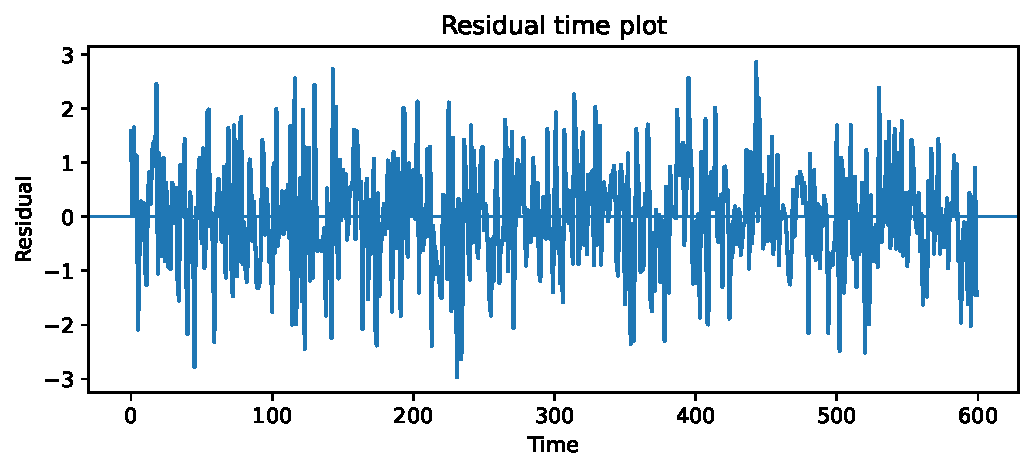
\includegraphics[keepaspectratio]{chapters/chapter-07-estimation-identification-diagnostics_files/figure-pdf/py-ch07-residual-diagnostics-output-2.pdf}}

}

\caption{Residual diagnostics for a fitted ARMA model.}

\end{figure}%

\pandocbounded{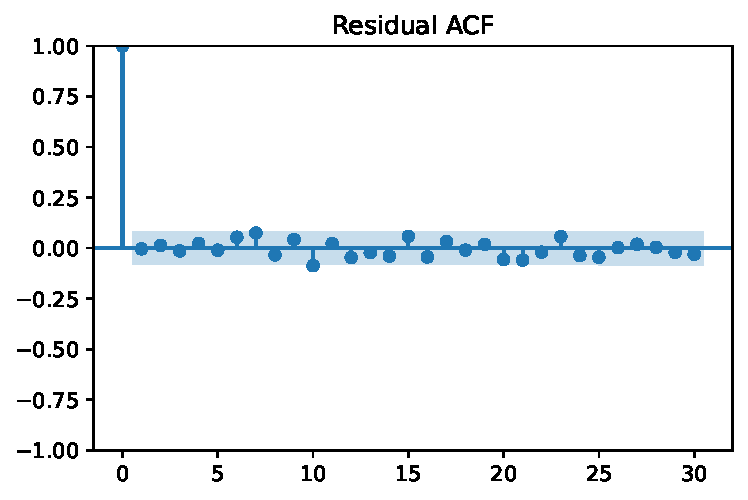
\includegraphics[keepaspectratio]{chapters/chapter-07-estimation-identification-diagnostics_files/figure-pdf/py-ch07-residual-diagnostics-output-3.pdf}}

\pandocbounded{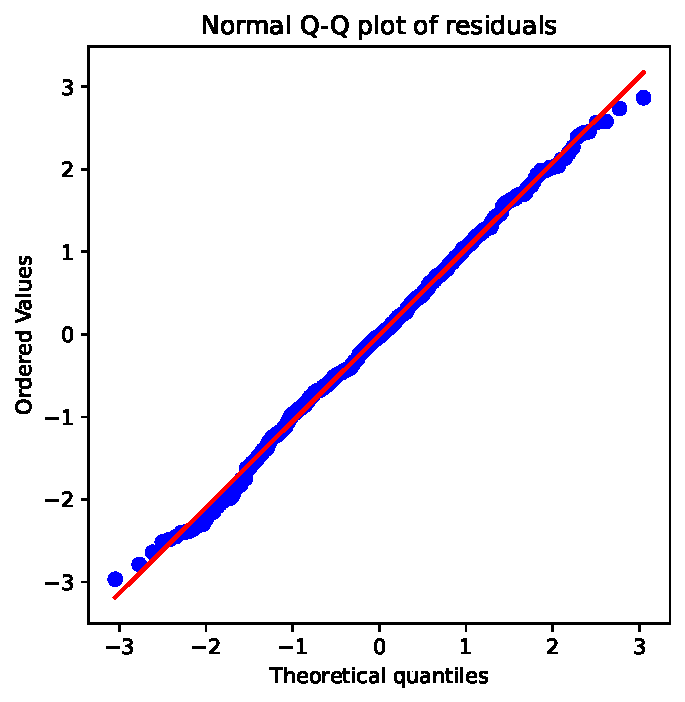
\includegraphics[keepaspectratio]{chapters/chapter-07-estimation-identification-diagnostics_files/figure-pdf/py-ch07-residual-diagnostics-output-4.pdf}}

\begin{tcolorbox}[enhanced jigsaw, arc=.35mm, bottomrule=.15mm, bottomtitle=1mm, breakable, colback=white, colbacktitle=quarto-callout-note-color!10!white, colframe=quarto-callout-note-color-frame, coltitle=black, left=2mm, leftrule=.75mm, opacityback=0, opacitybacktitle=0.6, rightrule=.15mm, title=\textcolor{quarto-callout-note-color}{\faInfo}\hspace{0.5em}{Reading the diagnostics}, titlerule=0mm, toprule=.15mm, toptitle=1mm]

A good residual time plot has no visible pattern. A good residual ACF
has no systematic significant autocorrelations. A good Q--Q plot is
approximately linear, although real data often have heavier tails than
the Gaussian model assumes.

\end{tcolorbox}

\section{7.15 Interactive HTML: residual diagnostics
laboratory}\label{interactive-html-residual-diagnostics-laboratory}

This module shows why residual diagnostics matter. White-noise
residuals, autocorrelated residuals, and heteroskedastic residuals can
look quite different.

\section{7.16 Python example: detecting changing
variance}\label{python-example-detecting-changing-variance}

A model can remove autocorrelation from the conditional mean but still
fail to model conditional variance. This is common in financial returns.

\protect\phantomsection\label{py-ch07-changing-variance}
\begin{Shaded}
\begin{Highlighting}[]
\NormalTok{np.random.seed(}\DecValTok{2027}\NormalTok{)}
\NormalTok{n }\OperatorTok{=} \DecValTok{600}
\NormalTok{z }\OperatorTok{=}\NormalTok{ np.random.normal(size}\OperatorTok{=}\NormalTok{n)}
\NormalTok{e }\OperatorTok{=}\NormalTok{ np.zeros(n)}
\ControlFlowTok{for}\NormalTok{ t }\KeywordTok{in} \BuiltInTok{range}\NormalTok{(}\DecValTok{1}\NormalTok{, n):}
\NormalTok{    sigma\_t }\OperatorTok{=}\NormalTok{ np.sqrt(}\FloatTok{0.2} \OperatorTok{+} \FloatTok{0.75} \OperatorTok{*}\NormalTok{ e[t}\OperatorTok{{-}}\DecValTok{1}\NormalTok{]}\OperatorTok{**}\DecValTok{2}\NormalTok{)}
\NormalTok{    e[t] }\OperatorTok{=}\NormalTok{ sigma\_t }\OperatorTok{*}\NormalTok{ z[t]}

\NormalTok{fig, ax }\OperatorTok{=}\NormalTok{ plt.subplots(figsize}\OperatorTok{=}\NormalTok{(}\DecValTok{8}\NormalTok{, }\DecValTok{3}\NormalTok{))}
\NormalTok{ax.plot(e)}
\NormalTok{ax.set\_title(}\StringTok{"Synthetic residuals with changing variance"}\NormalTok{)}
\NormalTok{ax.set\_xlabel(}\StringTok{"Time"}\NormalTok{)}
\NormalTok{ax.set\_ylabel(}\StringTok{"Residual"}\NormalTok{)}
\NormalTok{plt.show()}

\NormalTok{plot\_acf(e, lags}\OperatorTok{=}\DecValTok{30}\NormalTok{)}
\NormalTok{plt.title(}\StringTok{"ACF of residuals"}\NormalTok{)}
\NormalTok{plt.show()}

\NormalTok{plot\_acf(e}\OperatorTok{**}\DecValTok{2}\NormalTok{, lags}\OperatorTok{=}\DecValTok{30}\NormalTok{)}
\NormalTok{plt.title(}\StringTok{"ACF of squared residuals"}\NormalTok{)}
\NormalTok{plt.show()}
\end{Highlighting}
\end{Shaded}

\begin{figure}[H]

{\centering \pandocbounded{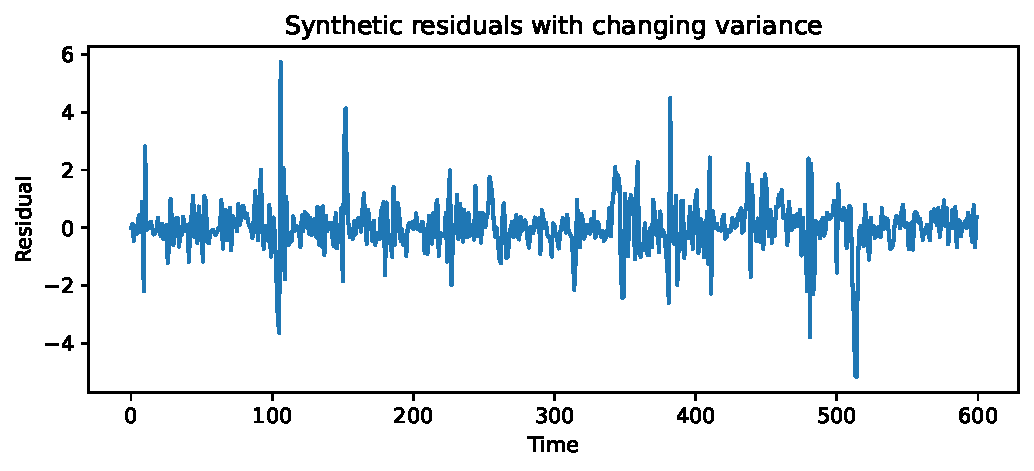
\includegraphics[keepaspectratio]{chapters/chapter-07-estimation-identification-diagnostics_files/figure-pdf/py-ch07-changing-variance-output-1.pdf}}

}

\caption{Changing variance can be visible in squared residuals even when
residual ACF is small.}

\end{figure}%

\pandocbounded{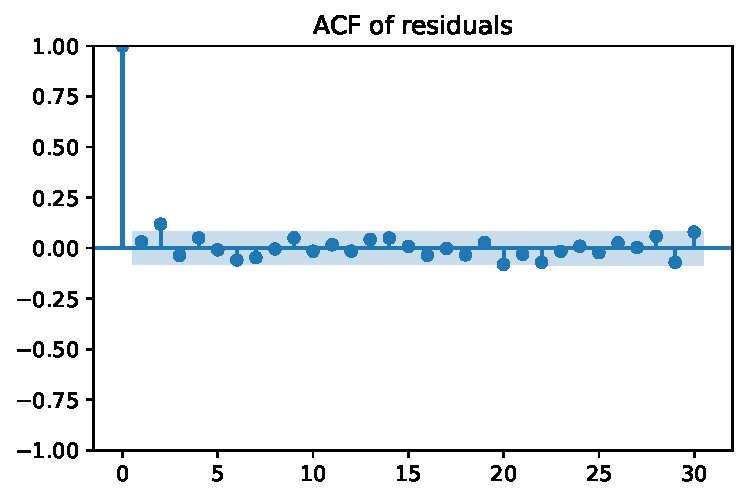
\includegraphics[keepaspectratio]{chapters/chapter-07-estimation-identification-diagnostics_files/figure-pdf/py-ch07-changing-variance-output-2.pdf}}

\pandocbounded{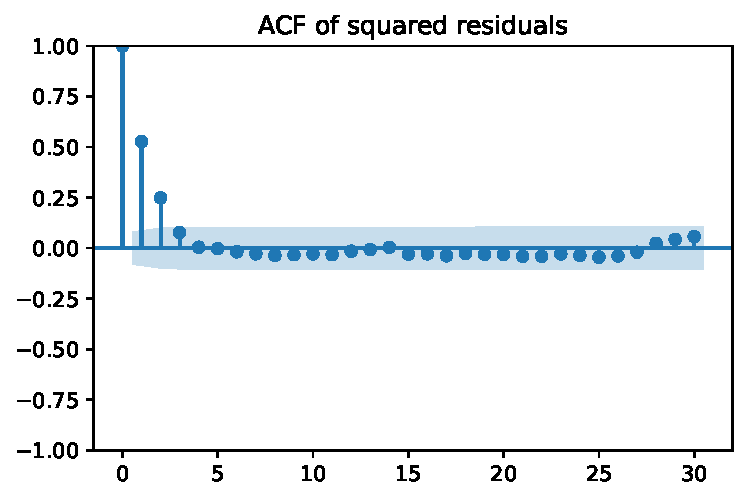
\includegraphics[keepaspectratio]{chapters/chapter-07-estimation-identification-diagnostics_files/figure-pdf/py-ch07-changing-variance-output-3.pdf}}

If the residual ACF is small but the squared residual ACF is large, the
conditional mean model may be adequate, but the variance model is not.
This motivates ARCH/GARCH models and modern volatility models.

\section{7.17 Forecasting and validation during model
selection}\label{forecasting-and-validation-during-model-selection}

Information criteria are computed in-sample. Forecasting performance
must be evaluated out-of-sample or by time-aware backtesting.

A simple time-series split is

\[
\underbrace{x_1,\ldots,x_T}_{\text{training}}
\quad
\underbrace{x_{T+1},\ldots,x_n}_{\text{testing}}.
\]

A rolling-origin evaluation repeatedly refits or updates the model at
increasing time origins:

\[
\{x_1,\ldots,x_T\}\rightarrow \widehat x_{T+h|T},
\]

\[
\{x_1,\ldots,x_{T+1}\}\rightarrow \widehat x_{T+1+h|T+1},
\]

and so on.

\begin{tcolorbox}[enhanced jigsaw, arc=.35mm, bottomrule=.15mm, bottomtitle=1mm, breakable, colback=white, colbacktitle=quarto-callout-warning-color!10!white, colframe=quarto-callout-warning-color-frame, coltitle=black, left=2mm, leftrule=.75mm, opacityback=0, opacitybacktitle=0.6, rightrule=.15mm, title=\textcolor{quarto-callout-warning-color}{\faExclamationTriangle}\hspace{0.5em}{Leakage warning}, titlerule=0mm, toprule=.15mm, toptitle=1mm]

Do not randomly shuffle a time series when evaluating a forecasting
model. Random splitting allows future information to leak into the
training set and gives overly optimistic performance.

\end{tcolorbox}

\section{7.18 AI-assisted model
criticism}\label{ai-assisted-model-criticism}

AI tools can be helpful in time-series modeling, but the mathematical
checks must remain explicit. The most useful role for AI is often
\textbf{critique}, not final authority.

\subsection{Productive AI prompts}\label{productive-ai-prompts}

Use prompts such as:

\begin{quote}
I fitted an ARMA(2,1) model. The residual ACF has significant spikes at
lags 7 and 14. Give possible mathematical explanations and suggest
diagnostics I should run next.
\end{quote}

\begin{quote}
Explain why choosing the model with the lowest AIC is not enough for a
final forecasting report.
\end{quote}

\begin{quote}
Here is my rolling-origin validation code. Identify possible time-series
leakage.
\end{quote}

\begin{quote}
My residuals are uncorrelated but have heavy tails. What changes affect
point forecasts, forecast intervals, or both?
\end{quote}

\subsection{Required verification}\label{required-verification}

Whenever an AI assistant suggests a model, verify the following
manually:

\begin{enumerate}
\def\labelenumi{\arabic{enumi}.}
\tightlist
\item
  Was stationarity checked before fitting stationary ARMA models?
\item
  Were transformations or differencing justified?
\item
  Are residuals approximately white noise?
\item
  Was model selection performed on comparable likelihoods?
\item
  Was forecast performance evaluated using a time-aware split?
\item
  Were uncertainty intervals calibrated or at least inspected?
\end{enumerate}

\begin{tcolorbox}[enhanced jigsaw, arc=.35mm, bottomrule=.15mm, bottomtitle=1mm, breakable, colback=white, colbacktitle=quarto-callout-important-color!10!white, colframe=quarto-callout-important-color-frame, coltitle=black, left=2mm, leftrule=.75mm, opacityback=0, opacitybacktitle=0.6, rightrule=.15mm, title=\textcolor{quarto-callout-important-color}{\faExclamation}\hspace{0.5em}{AI principle}, titlerule=0mm, toprule=.15mm, toptitle=1mm]

AI can suggest candidate explanations, but residual diagnostics and
forecasting validation decide whether the model is acceptable.

\end{tcolorbox}

\section{7.19 Common mistakes}\label{common-mistakes-6}

\begin{tcolorbox}[enhanced jigsaw, arc=.35mm, bottomrule=.15mm, bottomtitle=1mm, breakable, colback=white, colbacktitle=quarto-callout-caution-color!10!white, colframe=quarto-callout-caution-color-frame, coltitle=black, left=2mm, leftrule=.75mm, opacityback=0, opacitybacktitle=0.6, rightrule=.15mm, title=\textcolor{quarto-callout-caution-color}{\faFire}\hspace{0.5em}{Mistake 1: fitting ARMA to nonstationary data}, titlerule=0mm, toprule=.15mm, toptitle=1mm]

A slowly decaying ACF often indicates nonstationarity. Fitting a
stationary ARMA model without transformation or differencing can produce
misleading parameters.

\end{tcolorbox}

\begin{tcolorbox}[enhanced jigsaw, arc=.35mm, bottomrule=.15mm, bottomtitle=1mm, breakable, colback=white, colbacktitle=quarto-callout-caution-color!10!white, colframe=quarto-callout-caution-color-frame, coltitle=black, left=2mm, leftrule=.75mm, opacityback=0, opacitybacktitle=0.6, rightrule=.15mm, title=\textcolor{quarto-callout-caution-color}{\faFire}\hspace{0.5em}{Mistake 2: choosing the largest model}, titlerule=0mm, toprule=.15mm, toptitle=1mm]

A large ARMA model can reduce training error but produce unstable
forecasts and unnecessary parameter uncertainty.

\end{tcolorbox}

\begin{tcolorbox}[enhanced jigsaw, arc=.35mm, bottomrule=.15mm, bottomtitle=1mm, breakable, colback=white, colbacktitle=quarto-callout-caution-color!10!white, colframe=quarto-callout-caution-color-frame, coltitle=black, left=2mm, leftrule=.75mm, opacityback=0, opacitybacktitle=0.6, rightrule=.15mm, title=\textcolor{quarto-callout-caution-color}{\faFire}\hspace{0.5em}{Mistake 3: ignoring residual autocorrelation}, titlerule=0mm, toprule=.15mm, toptitle=1mm]

If residuals are autocorrelated, the fitted model has not fully captured
the dependence structure.

\end{tcolorbox}

\begin{tcolorbox}[enhanced jigsaw, arc=.35mm, bottomrule=.15mm, bottomtitle=1mm, breakable, colback=white, colbacktitle=quarto-callout-caution-color!10!white, colframe=quarto-callout-caution-color-frame, coltitle=black, left=2mm, leftrule=.75mm, opacityback=0, opacitybacktitle=0.6, rightrule=.15mm, title=\textcolor{quarto-callout-caution-color}{\faFire}\hspace{0.5em}{Mistake 4: using random train-test splits}, titlerule=0mm, toprule=.15mm, toptitle=1mm]

Random splits violate temporal ordering and create data leakage in
forecasting tasks.

\end{tcolorbox}

\begin{tcolorbox}[enhanced jigsaw, arc=.35mm, bottomrule=.15mm, bottomtitle=1mm, breakable, colback=white, colbacktitle=quarto-callout-caution-color!10!white, colframe=quarto-callout-caution-color-frame, coltitle=black, left=2mm, leftrule=.75mm, opacityback=0, opacitybacktitle=0.6, rightrule=.15mm, title=\textcolor{quarto-callout-caution-color}{\faFire}\hspace{0.5em}{Mistake 5: trusting software defaults without checking conventions}, titlerule=0mm, toprule=.15mm, toptitle=1mm]

Different packages use different likelihood approximations, trends,
intercepts, initialization methods, and parameter constraints.

\end{tcolorbox}

\section{7.20 Mini project: model identification
report}\label{mini-project-model-identification-report}

Choose one real or simulated stationary time series. Prepare a short
report with the following sections:

\begin{enumerate}
\def\labelenumi{\arabic{enumi}.}
\tightlist
\item
  time plot, ACF, and PACF;
\item
  candidate models and identification reasoning;
\item
  parameter estimates from at least two candidate models;
\item
  AIC, AICc, and BIC comparison;
\item
  residual time plot, residual ACF, Q--Q plot, and Ljung--Box test;
\item
  final model choice and explanation;
\item
  one-step and multi-step forecasts with uncertainty intervals;
\item
  a paragraph explaining what an AI assistant suggested and how you
  verified or rejected it.
\end{enumerate}

\section{7.21 Exercises}\label{exercises-6}

\subsection{Exercise 1}\label{exercise-1}

Let \(X_t=\phi X_{t-1}+W_t\) with \(|\phi|<1\). Derive the Yule--Walker
equation and show that

\[
\phi=\frac{\gamma(1)}{\gamma(0)}.
\]

\subsection{Exercise 2}\label{exercise-2}

For an AR(2) model, write the Yule--Walker system explicitly and solve
symbolically for \(\phi_1\) and \(\phi_2\) in terms of \(\gamma(0)\),
\(\gamma(1)\), and \(\gamma(2)\).

\subsection{Exercise 3}\label{exercise-3}

Suppose a fitted ARMA model has residual ACF spikes at lags 12, 24, and
36. Give at least two possible explanations and propose next modeling
steps.

\subsection{Exercise 4}\label{exercise-4}

Explain why AIC and BIC can select different models. Which criterion
penalizes complexity more strongly when \(n\) is large?

\subsection{Exercise 5}\label{exercise-5}

Simulate an MA(1) process with \(\theta=0.8\). Plot the ACF and PACF.
Does the ACF cut off exactly in the finite sample? Explain the
difference between theoretical and sample behavior.

\subsection{Exercise 6}\label{exercise-6}

Create a time series with changing variance but no autocorrelation in
the mean. Fit a mean-only model. Show that residual ACF may look
acceptable while squared residual ACF reveals dependence.

\subsection{Exercise 7}\label{exercise-7}

Write a short AI prompt asking for help diagnosing a poor ARIMA model.
Then write a checklist of what you would verify manually before trusting
the answer.

\section{7.22 Chapter checklist}\label{chapter-checklist-4}

By the end of this chapter, you should be able to:

\begin{itemize}
\tightlist
\item[$\square$]
  compute sample autocovariance and sample ACF;
\item[$\square$]
  use ACF/PACF patterns to propose candidate ARMA orders;
\item[$\square$]
  derive the Yule--Walker equations for AR(\(p\));
\item[$\square$]
  distinguish Yule--Walker, conditional least squares, and maximum
  likelihood;
\item[$\square$]
  use AIC, AICc, and BIC appropriately;
\item[$\square$]
  diagnose residual autocorrelation using plots and Ljung--Box tests;
\item[$\square$]
  recognize changing variance through squared residuals;
\item[$\square$]
  avoid leakage in time-series validation;
\item[$\square$]
  use AI as a model critic while verifying all claims mathematically and
  computationally.
\end{itemize}

\part{Part III. Nonstationary and Seasonal Models}

\chapter{ARIMA Models and
Differencing}\label{arima-models-and-differencing}

\textbf{Part III. Nonstationary and Seasonal Models}\\
\textbf{Chapter goal:} learn how to model nonstationary time series by
transforming them into stationary series. We develop differencing
operators, integrated processes, ARIMA models, model identification
after differencing, forecasting on the original scale, diagnostics, and
AI-assisted checks for under-differencing and over-differencing.

\section{Learning objectives}\label{learning-objectives-7}

After studying this chapter, you should be able to:

\begin{enumerate}
\def\labelenumi{\arabic{enumi}.}
\tightlist
\item
  explain why many real time series are nonstationary and why ARMA
  models cannot be applied directly;
\item
  use the backshift operator \(B\) and the difference operator
  \(\nabla=1-B\);
\item
  define ARIMA(\(p,d,q\)) models and interpret \(p\), \(d\), and \(q\);
\item
  distinguish deterministic trends from stochastic trends;
\item
  identify when first or second differencing is appropriate;
\item
  recognize over-differencing and under-differencing from time plots and
  ACF behavior;
\item
  use ACF and PACF of the differenced series to propose \(p\) and \(q\);
\item
  fit ARIMA models in Python and diagnose residuals;
\item
  transform forecasts of differenced data back to forecasts of the
  original series;
\item
  use AI tools to critique a proposed ARIMA workflow while verifying all
  mathematical and diagnostic claims.
\end{enumerate}

\section{8.1 Why ARIMA is needed}\label{why-arima-is-needed}

So far, the core linear model class has been ARMA(\(p,q\)):

\[
\phi(B)X_t=\theta(B)W_t,
\]

where \(\{X_t\}\) is assumed stationary. This assumption is powerful
because it lets us summarize dependence using a time-invariant
autocovariance function

\[
\gamma(h)=\operatorname{Cov}(X_{t+h},X_t),
\]

and a time-invariant autocorrelation function

\[
\rho(h)=\frac{\gamma(h)}{\gamma(0)}.
\]

However, many real time series are not stationary. A stock index,
cumulative sales, population count, temperature anomaly, ridership
total, or electricity demand series may have trend, changing level,
seasonality, or structural changes. Applying a stationary ARMA model
directly to such a series often produces misleading forecasts and
misleading standard errors.

ARIMA models solve one important kind of nonstationarity by
\textbf{differencing}. Instead of assuming \(X_t\) itself is stationary,
we assume that a differenced version of \(X_t\) is stationary.

\begin{tcolorbox}[enhanced jigsaw, arc=.35mm, bottomrule=.15mm, bottomtitle=1mm, breakable, colback=white, colbacktitle=quarto-callout-note-color!10!white, colframe=quarto-callout-note-color-frame, coltitle=black, left=2mm, leftrule=.75mm, opacityback=0, opacitybacktitle=0.6, rightrule=.15mm, title=\textcolor{quarto-callout-note-color}{\faInfo}\hspace{0.5em}{Core idea}, titlerule=0mm, toprule=.15mm, toptitle=1mm]

An ARIMA model is an ARMA model applied after differencing:

\[
\nabla^d X_t \quad \text{is modeled as ARMA}(p,q).
\]

\end{tcolorbox}

This idea is simple but subtle. Differencing can remove trend, but it
also changes the dependence structure. Choosing the differencing order
\(d\) is therefore a modeling decision, not a mechanical preprocessing
step.

\section{8.2 Backshift and difference
operators}\label{backshift-and-difference-operators}

The \textbf{backshift operator} \(B\) acts on a time series by shifting
it one time step backward:

\[
BX_t=X_{t-1}.
\]

The first difference operator is

\[
\nabla X_t=X_t-X_{t-1}=(1-B)X_t.
\]

The second difference is

\[
\nabla^2X_t=\nabla(\nabla X_t)=(1-B)^2X_t.
\]

Expanding gives

\[
\nabla^2X_t=X_t-2X_{t-1}+X_{t-2}.
\]

More generally,

\[
\nabla^dX_t=(1-B)^dX_t.
\]

Using the binomial theorem,

\[
(1-B)^d = \sum_{j=0}^{d} {d \choose j}(-1)^j B^j,
\]

so

\[
\nabla^dX_t=\sum_{j=0}^{d}{d \choose j}(-1)^jX_{t-j}.
\]

For example,

\[
\nabla^3X_t=X_t-3X_{t-1}+3X_{t-2}-X_{t-3}.
\]

In practice, we rarely use \(d>2\) for ordinary nonseasonal
differencing. Large \(d\) can create artificial negative autocorrelation
and unnecessarily complex models.

\begin{tcolorbox}[enhanced jigsaw, arc=.35mm, bottomrule=.15mm, bottomtitle=1mm, breakable, colback=white, colbacktitle=quarto-callout-warning-color!10!white, colframe=quarto-callout-warning-color-frame, coltitle=black, left=2mm, leftrule=.75mm, opacityback=0, opacitybacktitle=0.6, rightrule=.15mm, title=\textcolor{quarto-callout-warning-color}{\faExclamationTriangle}\hspace{0.5em}{Practical warning}, titlerule=0mm, toprule=.15mm, toptitle=1mm]

Differencing is not harmless. It removes low-frequency behavior, but it
also changes the stochastic part of the series. Over-differencing can
turn a simple signal into a noisier signal with avoidable moving-average
structure.

\end{tcolorbox}

\section{8.3 Deterministic trend versus stochastic
trend}\label{deterministic-trend-versus-stochastic-trend}

A common model for a nonstationary-looking series is

\[
X_t=\mu_t+Y_t,
\]

where \(\mu_t\) is a deterministic trend and \(Y_t\) is stationary. For
example,

\[
X_t=\beta_0+\beta_1t+Y_t.
\]

Then

\[
\nabla X_t=X_t-X_{t-1}
=\beta_1+Y_t-Y_{t-1}.
\]

If \(Y_t\) is stationary, then \(Y_t-Y_{t-1}\) is also stationary.
Therefore, the first difference is stationary around mean \(\beta_1\).

But there is another kind of nonstationarity: a \textbf{stochastic
trend}. The random walk is the basic example:

\[
X_t=X_{t-1}+W_t,
\]

where \(W_t\sim WN(0,\sigma^2)\). Then

\[
\nabla X_t=W_t,
\]

which is stationary white noise. The original process is nonstationary
because

\[
\operatorname{Var}(X_t)=t\sigma^2
\]

when \(X_0=0\).

These two cases can look similar in a time plot but have different
interpretations.

{\def\LTcaptype{none} % do not increment counter
\begin{longtable}[]{@{}
  >{\raggedright\arraybackslash}p{(\linewidth - 6\tabcolsep) * \real{0.2500}}
  >{\raggedright\arraybackslash}p{(\linewidth - 6\tabcolsep) * \real{0.2500}}
  >{\raggedright\arraybackslash}p{(\linewidth - 6\tabcolsep) * \real{0.2500}}
  >{\raggedright\arraybackslash}p{(\linewidth - 6\tabcolsep) * \real{0.2500}}@{}}
\toprule\noalign{}
\begin{minipage}[b]{\linewidth}\raggedright
Type
\end{minipage} & \begin{minipage}[b]{\linewidth}\raggedright
Example
\end{minipage} & \begin{minipage}[b]{\linewidth}\raggedright
What differencing does
\end{minipage} & \begin{minipage}[b]{\linewidth}\raggedright
Interpretation
\end{minipage} \\
\midrule\noalign{}
\endhead
\bottomrule\noalign{}
\endlastfoot
Deterministic trend & \(X_t=\beta_0+\beta_1t+Y_t\) & removes the linear
trend & series fluctuates around a deterministic path \\
Stochastic trend & \(X_t=X_{t-1}+W_t\) & removes the unit root & shocks
have permanent effects \\
\end{longtable}
}

\begin{tcolorbox}[enhanced jigsaw, arc=.35mm, bottomrule=.15mm, bottomtitle=1mm, breakable, colback=white, colbacktitle=quarto-callout-tip-color!10!white, colframe=quarto-callout-tip-color-frame, coltitle=black, left=2mm, leftrule=.75mm, opacityback=0, opacitybacktitle=0.6, rightrule=.15mm, title=\textcolor{quarto-callout-tip-color}{\faLightbulb}\hspace{0.5em}{Modeling interpretation}, titlerule=0mm, toprule=.15mm, toptitle=1mm]

A deterministic trend says the long-run path is predictable up to
stationary noise. A stochastic trend says shocks accumulate and
permanently change the level.

\end{tcolorbox}

\section{8.4 Integrated processes}\label{integrated-processes}

A process \(X_t\) is called \textbf{integrated of order \(d\)}, written
\(X_t\sim I(d)\), if

\[
\nabla^d X_t
\]

is stationary, while \(\nabla^{d-1}X_t\) is not stationary.

Examples:

\begin{enumerate}
\def\labelenumi{\arabic{enumi}.}
\tightlist
\item
  White noise is \(I(0)\).
\item
  A stationary ARMA process is \(I(0)\).
\item
  A random walk is \(I(1)\).
\item
  A process whose second difference is stationary but whose first
  difference is not stationary is \(I(2)\).
\end{enumerate}

The notation \(I(d)\) is about the number of differences needed to reach
stationarity. It is not a statement that the original series has finite
variance for all time. In fact, many integrated processes are
nonstationary and have variance that grows with time.

\section{\texorpdfstring{8.5 Definition of
ARIMA(\(p,d,q\))}{8.5 Definition of ARIMA(p,d,q)}}\label{definition-of-arimapdq}

A time series \(\{X_t\}\) is an ARIMA(\(p,d,q\)) process if

\[
Y_t=\nabla^dX_t=(1-B)^dX_t
\]

is an ARMA(\(p,q\)) process. That is,

\[
\phi(B)Y_t=\theta(B)W_t,
\]

where

\[
\phi(B)=1-\phi_1B-\cdots-\phi_pB^p,
\]

and

\[
\theta(B)=1+\theta_1B+\cdots+\theta_qB^q.
\]

Substituting \(Y_t=(1-B)^dX_t\) gives the ARIMA equation

\[
\phi(B)(1-B)^dX_t=\theta(B)W_t.
\]

If the differenced series has a nonzero mean, we write

\[
\phi(B)(1-B)^dX_t=\alpha+\theta(B)W_t.
\]

The three orders have different meanings:

{\def\LTcaptype{none} % do not increment counter
\begin{longtable}[]{@{}
  >{\raggedright\arraybackslash}p{(\linewidth - 4\tabcolsep) * \real{0.3333}}
  >{\raggedright\arraybackslash}p{(\linewidth - 4\tabcolsep) * \real{0.3333}}
  >{\raggedright\arraybackslash}p{(\linewidth - 4\tabcolsep) * \real{0.3333}}@{}}
\toprule\noalign{}
\begin{minipage}[b]{\linewidth}\raggedright
Symbol
\end{minipage} & \begin{minipage}[b]{\linewidth}\raggedright
Meaning
\end{minipage} & \begin{minipage}[b]{\linewidth}\raggedright
Role
\end{minipage} \\
\midrule\noalign{}
\endhead
\bottomrule\noalign{}
\endlastfoot
\(p\) & autoregressive order & dependence on past differenced values \\
\(d\) & differencing order & number of nonseasonal differences needed
for stationarity \\
\(q\) & moving-average order & dependence on past shocks/innovations \\
\end{longtable}
}

\begin{tcolorbox}[enhanced jigsaw, arc=.35mm, bottomrule=.15mm, bottomtitle=1mm, breakable, colback=white, colbacktitle=quarto-callout-note-color!10!white, colframe=quarto-callout-note-color-frame, coltitle=black, left=2mm, leftrule=.75mm, opacityback=0, opacitybacktitle=0.6, rightrule=.15mm, title=\textcolor{quarto-callout-note-color}{\faInfo}\hspace{0.5em}{ARMA as a special case}, titlerule=0mm, toprule=.15mm, toptitle=1mm]

ARMA(\(p,q\)) is the same as ARIMA(\(p,0,q\)). ARIMA extends ARMA by
allowing integrated nonstationarity.

\end{tcolorbox}

\section{8.6 Basic examples}\label{basic-examples-1}

\subsection{Example 1: White noise}\label{example-1-white-noise}

If

\[
X_t=W_t,
\]

then \(X_t\) is ARIMA(\(0,0,0\)). No differencing is needed.

\subsection{Example 2: Random walk}\label{example-2-random-walk}

If

\[
X_t=X_{t-1}+W_t,
\]

then

\[
(1-B)X_t=W_t.
\]

Thus \(X_t\) is ARIMA(\(0,1,0\)).

\subsection{Example 3: Random walk with
drift}\label{example-3-random-walk-with-drift}

If

\[
X_t=\delta+X_{t-1}+W_t,
\]

then

\[
\nabla X_t=\delta+W_t.
\]

This is ARIMA(\(0,1,0\)) with drift. The \(h\)-step forecast from time
\(n\) is

\[
\widehat X_{n+h|n}=X_n+h\widehat\delta.
\]

\subsection{\texorpdfstring{Example 4:
ARIMA(\(1,1,0\))}{Example 4: ARIMA(1,1,0)}}\label{example-4-arima110}

If

\[
\nabla X_t=\phi \nabla X_{t-1}+W_t,
\]

then

\[
(1-\phi B)(1-B)X_t=W_t.
\]

This is ARIMA(\(1,1,0\)). The first differences behave like an AR(1)
process.

\subsection{\texorpdfstring{Example 5:
ARIMA(\(0,1,1\))}{Example 5: ARIMA(0,1,1)}}\label{example-5-arima011}

If

\[
\nabla X_t=W_t+\theta W_{t-1},
\]

then

\[
(1-B)X_t=(1+\theta B)W_t.
\]

This is ARIMA(\(0,1,1\)). Some exponential smoothing models are closely
related to ARIMA(\(0,1,1\)).

\section{8.7 Differencing a deterministic
trend}\label{differencing-a-deterministic-trend}

Suppose

\[
X_t=\beta_0+\beta_1t+Y_t,
\]

where \(Y_t\) is stationary. Then

\[
\nabla X_t=\beta_1+(Y_t-Y_{t-1}).
\]

This is stationary if \(Y_t\) is stationary. But notice that the noise
structure has changed. If \(Y_t\) is white noise, then

\[
Y_t-Y_{t-1}=W_t-W_{t-1},
\]

which is MA(1) with coefficient \(-1\).

This explains a common phenomenon: differencing a deterministic trend
often creates moving-average behavior.

For a quadratic trend,

\[
X_t=\beta_0+\beta_1t+\beta_2t^2+Y_t,
\]

the first difference still has a linear trend:

\[
\nabla X_t=\beta_1+\beta_2(2t-1)+Y_t-Y_{t-1}.
\]

The second difference removes the quadratic trend:

\[
\nabla^2 X_t=2\beta_2+Y_t-2Y_{t-1}+Y_{t-2}.
\]

\begin{tcolorbox}[enhanced jigsaw, arc=.35mm, bottomrule=.15mm, bottomtitle=1mm, breakable, colback=white, colbacktitle=quarto-callout-warning-color!10!white, colframe=quarto-callout-warning-color-frame, coltitle=black, left=2mm, leftrule=.75mm, opacityback=0, opacitybacktitle=0.6, rightrule=.15mm, title=\textcolor{quarto-callout-warning-color}{\faExclamationTriangle}\hspace{0.5em}{Detrending versus differencing}, titlerule=0mm, toprule=.15mm, toptitle=1mm]

Regression detrending estimates and subtracts \(\widehat\mu_t\).
Differencing removes polynomial trend without estimating all trend
coefficients, but it changes the stationary component. Both tools are
useful, and neither should be applied blindly.

\end{tcolorbox}

\section{\texorpdfstring{8.8 How to choose the differencing order
\(d\)}{8.8 How to choose the differencing order d}}\label{how-to-choose-the-differencing-order-d}

The differencing order \(d\) should be chosen before identifying \(p\)
and \(q\). The usual workflow is:

\begin{enumerate}
\def\labelenumi{\arabic{enumi}.}
\tightlist
\item
  Plot \(X_t\).
\item
  Check whether the level and variance appear stable.
\item
  Inspect the ACF of \(X_t\).
\item
  Difference once and inspect \(\nabla X_t\).
\item
  Difference twice only if necessary.
\item
  Once the differenced series appears stationary, inspect ACF/PACF to
  choose \(p\) and \(q\).
\end{enumerate}

A slowly decaying ACF is a common sign of nonstationarity. For a random
walk or a strongly trended series, the sample ACF often remains large
for many lags.

Typical clues:

{\def\LTcaptype{none} % do not increment counter
\begin{longtable}[]{@{}
  >{\raggedright\arraybackslash}p{(\linewidth - 2\tabcolsep) * \real{0.5000}}
  >{\raggedright\arraybackslash}p{(\linewidth - 2\tabcolsep) * \real{0.5000}}@{}}
\toprule\noalign{}
\begin{minipage}[b]{\linewidth}\raggedright
Observation
\end{minipage} & \begin{minipage}[b]{\linewidth}\raggedright
Possible decision
\end{minipage} \\
\midrule\noalign{}
\endhead
\bottomrule\noalign{}
\endlastfoot
time plot has stable level and variance & try \(d=0\) \\
time plot has persistent trend & try \(d=1\) \\
first difference still has trend & consider \(d=2\) \\
ACF decays very slowly & increase \(d\) or remove trend \\
lag-1 ACF of differenced series is strongly negative & possible
over-differencing \\
\end{longtable}
}

Formal tests can help, but they do not replace plots and subject-matter
reasoning. Two common tests are:

\begin{itemize}
\tightlist
\item
  the augmented Dickey--Fuller test, where the null hypothesis is often
  a unit root;
\item
  the KPSS test, where the null hypothesis is often stationarity around
  a level or trend.
\end{itemize}

These tests can disagree in finite samples. For this course, the key
principle is to combine mathematical structure, plots, ACF/PACF,
residual diagnostics, and forecasting performance.

\section{8.9 Under-differencing and
over-differencing}\label{under-differencing-and-over-differencing}

\subsection{Under-differencing}\label{under-differencing}

A series is under-differenced if nonstationarity remains after
transformation. Symptoms include:

\begin{itemize}
\tightlist
\item
  a visible trend in the transformed series;
\item
  slowly decaying ACF;
\item
  residual autocorrelation after fitting;
\item
  forecasts that lag behind changes in level.
\end{itemize}

\subsection{Over-differencing}\label{over-differencing}

A series is over-differenced if too many differences are applied.
Symptoms include:

\begin{itemize}
\tightlist
\item
  unnecessary roughness;
\item
  strong negative autocorrelation at lag 1;
\item
  inflated forecast variance;
\item
  fitted MA coefficients near noninvertibility;
\item
  worse out-of-sample forecasts despite apparently stationary
  transformed data.
\end{itemize}

A simple example shows why. If \(X_t\) is already white noise, then

\[
Y_t=\nabla X_t=X_t-X_{t-1}=W_t-W_{t-1}.
\]

This is MA(1) with coefficient \(-1\). Its lag-1 autocorrelation is

\[
\rho_Y(1)=\frac{-\sigma^2}{2\sigma^2}=-\frac12.
\]

Thus differencing white noise creates artificial negative dependence.

\begin{tcolorbox}[enhanced jigsaw, arc=.35mm, bottomrule=.15mm, bottomtitle=1mm, breakable, colback=white, colbacktitle=quarto-callout-tip-color!10!white, colframe=quarto-callout-tip-color-frame, coltitle=black, left=2mm, leftrule=.75mm, opacityback=0, opacitybacktitle=0.6, rightrule=.15mm, title=\textcolor{quarto-callout-tip-color}{\faLightbulb}\hspace{0.5em}{Diagnostic rule of thumb}, titlerule=0mm, toprule=.15mm, toptitle=1mm]

If the differenced series has a very negative lag-1 autocorrelation, ask
whether the original series may have been differenced too much.

\end{tcolorbox}

\section{\texorpdfstring{8.10 Identifying \(p\) and \(q\) after
differencing}{8.10 Identifying p and q after differencing}}\label{identifying-p-and-q-after-differencing}

Once \(Y_t=\nabla^dX_t\) looks stationary, identify the ARMA model for
\(Y_t\).

For \(Y_t\):

{\def\LTcaptype{none} % do not increment counter
\begin{longtable}[]{@{}lll@{}}
\toprule\noalign{}
Candidate for \(Y_t\) & ACF & PACF \\
\midrule\noalign{}
\endhead
\bottomrule\noalign{}
\endlastfoot
AR(\(p\)) & decays gradually & cuts off after lag \(p\) \\
MA(\(q\)) & cuts off after lag \(q\) & decays gradually \\
ARMA(\(p,q\)) & decays gradually & decays gradually \\
white noise & insignificant after lag 0 & insignificant after lag 0 \\
\end{longtable}
}

Then \(X_t\) is ARIMA(\(p,d,q\)).

Example: If \(\nabla X_t\) has an ACF that cuts off after lag 1 and a
PACF that decays gradually, then \(\nabla X_t\) may be MA(1), so \(X_t\)
may be ARIMA(\(0,1,1\)).

Example: If \(\nabla X_t\) has a PACF that cuts off after lag 2 and an
ACF that decays gradually, then \(\nabla X_t\) may be AR(2), so \(X_t\)
may be ARIMA(\(2,1,0\)).

\section{8.11 Forecasting ARIMA models}\label{forecasting-arima-models}

Forecasting an ARIMA model happens in two stages:

\begin{enumerate}
\def\labelenumi{\arabic{enumi}.}
\tightlist
\item
  Forecast the stationary differenced series.
\item
  Convert the forecast back to the original scale.
\end{enumerate}

For ARIMA(\(p,1,q\)), define

\[
Y_t=\nabla X_t=X_t-X_{t-1}.
\]

Suppose we forecast future differences:

\[
\widehat Y_{n+1|n},\widehat Y_{n+2|n},\ldots,\widehat Y_{n+h|n}.
\]

Then forecasts of the original series satisfy

\[
\widehat X_{n+1|n}=X_n+\widehat Y_{n+1|n},
\]

\[
\widehat X_{n+2|n}=\widehat X_{n+1|n}+\widehat Y_{n+2|n},
\]

and in general

\[
\widehat X_{n+h|n}=X_n+\sum_{j=1}^{h}\widehat Y_{n+j|n}.
\]

For \(d=2\), the reconstruction accumulates second-difference forecasts
twice. Software handles this automatically, but students should
understand that ARIMA forecasts are produced by modeling changes and
then integrating the forecasted changes.

\begin{tcolorbox}[enhanced jigsaw, arc=.35mm, bottomrule=.15mm, bottomtitle=1mm, breakable, colback=white, colbacktitle=quarto-callout-note-color!10!white, colframe=quarto-callout-note-color-frame, coltitle=black, left=2mm, leftrule=.75mm, opacityback=0, opacitybacktitle=0.6, rightrule=.15mm, title=\textcolor{quarto-callout-note-color}{\faInfo}\hspace{0.5em}{Forecast intervals widen}, titlerule=0mm, toprule=.15mm, toptitle=1mm]

Integrated models often produce forecast intervals that widen with
horizon because future shocks accumulate on the original scale.

\end{tcolorbox}

\section{8.12 Constants, drift, and trend in
ARIMA}\label{constants-drift-and-trend-in-arima}

Constants in ARIMA models require care. Consider

\[
\phi(B)(1-B)^dX_t=\alpha+\theta(B)W_t.
\]

When \(d=0\), a constant usually corresponds to a nonzero mean of the
stationary ARMA process.

When \(d=1\), a constant in the differenced equation corresponds to
drift in the original series. For example,

\[
\nabla X_t=\delta+W_t
\]

implies

\[
X_t=X_0+\delta t+\sum_{j=1}^{t}W_j.
\]

Thus \(\delta\) creates a linear mean path on the original scale.

When \(d=2\), a constant in the second-differenced equation can induce a
quadratic mean path on the original scale. This is one reason to avoid
high differencing orders unless there is a clear reason.

\section{8.13 Model estimation and
diagnostics}\label{model-estimation-and-diagnostics}

An ARIMA workflow usually follows these steps:

\begin{enumerate}
\def\labelenumi{\arabic{enumi}.}
\tightlist
\item
  Transform the data if needed, such as log transform for increasing
  variance.
\item
  Choose \(d\) using plots, ACF, and domain knowledge.
\item
  Inspect ACF/PACF of \(\nabla^dX_t\) to propose \(p\) and \(q\).
\item
  Fit several candidate ARIMA models.
\item
  Compare using AIC, AICc, BIC, and forecast validation.
\item
  Check residuals.
\item
  Revise if residuals show autocorrelation, changing variance, outliers,
  or nonnormal heavy tails.
\item
  Forecast and communicate uncertainty.
\end{enumerate}

Residuals should behave like white noise:

\[
\widehat e_t \approx WN(0,\sigma^2).
\]

Useful residual diagnostics include:

\begin{itemize}
\tightlist
\item
  residual time plot;
\item
  residual ACF;
\item
  Ljung--Box test;
\item
  histogram and Q--Q plot;
\item
  rolling variance check;
\item
  forecast backtesting.
\end{itemize}

\begin{tcolorbox}[enhanced jigsaw, arc=.35mm, bottomrule=.15mm, bottomtitle=1mm, breakable, colback=white, colbacktitle=quarto-callout-warning-color!10!white, colframe=quarto-callout-warning-color-frame, coltitle=black, left=2mm, leftrule=.75mm, opacityback=0, opacitybacktitle=0.6, rightrule=.15mm, title=\textcolor{quarto-callout-warning-color}{\faExclamationTriangle}\hspace{0.5em}{Do not choose by AIC alone}, titlerule=0mm, toprule=.15mm, toptitle=1mm]

AIC can help compare fitted candidate models, but a model with the
lowest AIC may still have bad residual diagnostics or poor forecasting
performance on future data.

\end{tcolorbox}

\section{8.14 Interactive HTML: Differencing
explorer}\label{interactive-html-differencing-explorer}

Use this module to see how trend, a unit-root component, and stationary
AR noise affect the original and differenced series. The ACF plot
updates after applying \(d=0\), \(d=1\), or \(d=2\) differences.

\section{8.15 Python example: deterministic trend, random walk, and
differencing}\label{python-example-deterministic-trend-random-walk-and-differencing}

The following example compares deterministic and stochastic trend. Both
can look nonstationary, but their meanings are different.

\protect\phantomsection\label{py-ch08-deterministic-vs-stochastic-trend}
\begin{Shaded}
\begin{Highlighting}[]
\ImportTok{import}\NormalTok{ numpy }\ImportTok{as}\NormalTok{ np}
\ImportTok{import}\NormalTok{ matplotlib.pyplot }\ImportTok{as}\NormalTok{ plt}

\NormalTok{np.random.seed(}\DecValTok{7339}\NormalTok{)}

\NormalTok{n }\OperatorTok{=} \DecValTok{250}
\NormalTok{t }\OperatorTok{=}\NormalTok{ np.arange(n)}

\CommentTok{\# Deterministic trend plus stationary noise}
\NormalTok{phi }\OperatorTok{=} \FloatTok{0.6}
\NormalTok{noise }\OperatorTok{=}\NormalTok{ np.random.normal(size}\OperatorTok{=}\NormalTok{n)}
\NormalTok{y }\OperatorTok{=}\NormalTok{ np.zeros(n)}
\ControlFlowTok{for}\NormalTok{ i }\KeywordTok{in} \BuiltInTok{range}\NormalTok{(}\DecValTok{1}\NormalTok{, n):}
\NormalTok{    y[i] }\OperatorTok{=}\NormalTok{ phi }\OperatorTok{*}\NormalTok{ y[i}\OperatorTok{{-}}\DecValTok{1}\NormalTok{] }\OperatorTok{+}\NormalTok{ noise[i]}

\NormalTok{x\_det }\OperatorTok{=} \DecValTok{10} \OperatorTok{+} \FloatTok{0.05} \OperatorTok{*}\NormalTok{ t }\OperatorTok{+}\NormalTok{ y}

\CommentTok{\# Stochastic trend: random walk with drift}
\NormalTok{w }\OperatorTok{=}\NormalTok{ np.random.normal(scale}\OperatorTok{=}\FloatTok{1.0}\NormalTok{, size}\OperatorTok{=}\NormalTok{n)}
\NormalTok{x\_rw }\OperatorTok{=}\NormalTok{ np.cumsum(}\FloatTok{0.05} \OperatorTok{+}\NormalTok{ w)}

\NormalTok{fig, ax }\OperatorTok{=}\NormalTok{ plt.subplots(figsize}\OperatorTok{=}\NormalTok{(}\DecValTok{9}\NormalTok{, }\FloatTok{3.5}\NormalTok{))}
\NormalTok{ax.plot(t, x\_det, label}\OperatorTok{=}\StringTok{"deterministic trend + AR(1)"}\NormalTok{)}
\NormalTok{ax.plot(t, x\_rw, label}\OperatorTok{=}\StringTok{"random walk with drift"}\NormalTok{)}
\NormalTok{ax.set\_title(}\StringTok{"Two nonstationary{-}looking series"}\NormalTok{)}
\NormalTok{ax.set\_xlabel(}\StringTok{"time"}\NormalTok{)}
\NormalTok{ax.legend()}
\NormalTok{plt.show()}

\NormalTok{fig, ax }\OperatorTok{=}\NormalTok{ plt.subplots(figsize}\OperatorTok{=}\NormalTok{(}\DecValTok{9}\NormalTok{, }\FloatTok{3.5}\NormalTok{))}
\NormalTok{ax.plot(t[}\DecValTok{1}\NormalTok{:], np.diff(x\_det), label}\OperatorTok{=}\StringTok{"difference of deterministic trend model"}\NormalTok{)}
\NormalTok{ax.plot(t[}\DecValTok{1}\NormalTok{:], np.diff(x\_rw), label}\OperatorTok{=}\StringTok{"difference of random walk"}\NormalTok{)}
\NormalTok{ax.axhline(}\DecValTok{0}\NormalTok{, linewidth}\OperatorTok{=}\DecValTok{1}\NormalTok{)}
\NormalTok{ax.set\_title(}\StringTok{"First differences"}\NormalTok{)}
\NormalTok{ax.set\_xlabel(}\StringTok{"time"}\NormalTok{)}
\NormalTok{ax.legend()}
\NormalTok{plt.show()}
\end{Highlighting}
\end{Shaded}

\begin{figure}[H]

{\centering \pandocbounded{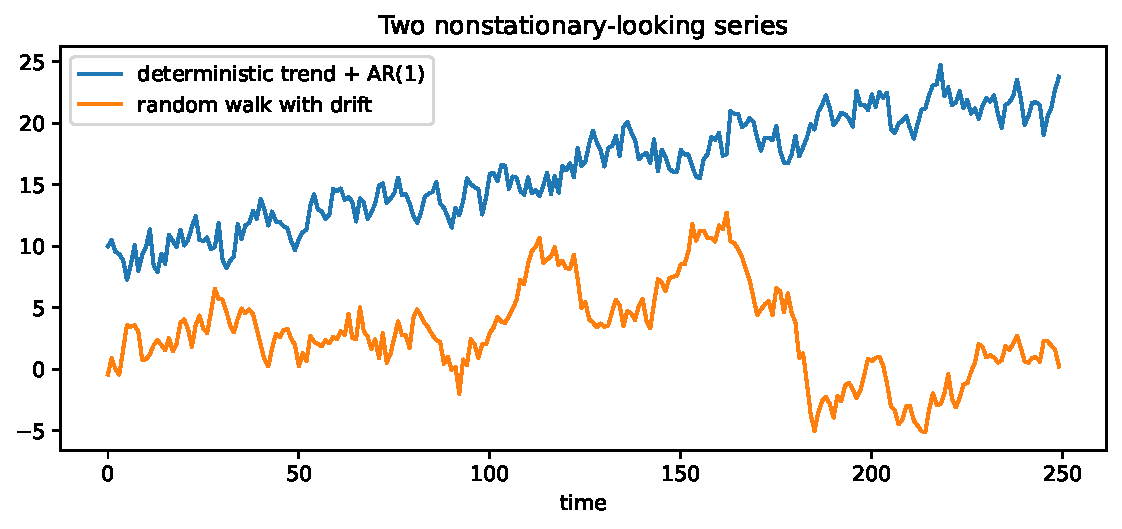
\includegraphics[keepaspectratio]{chapters/chapter-08-arima-differencing_files/figure-pdf/py-ch08-deterministic-vs-stochastic-trend-output-1.pdf}}

}

\caption{Deterministic trend and stochastic trend before and after
differencing.}

\end{figure}%

\pandocbounded{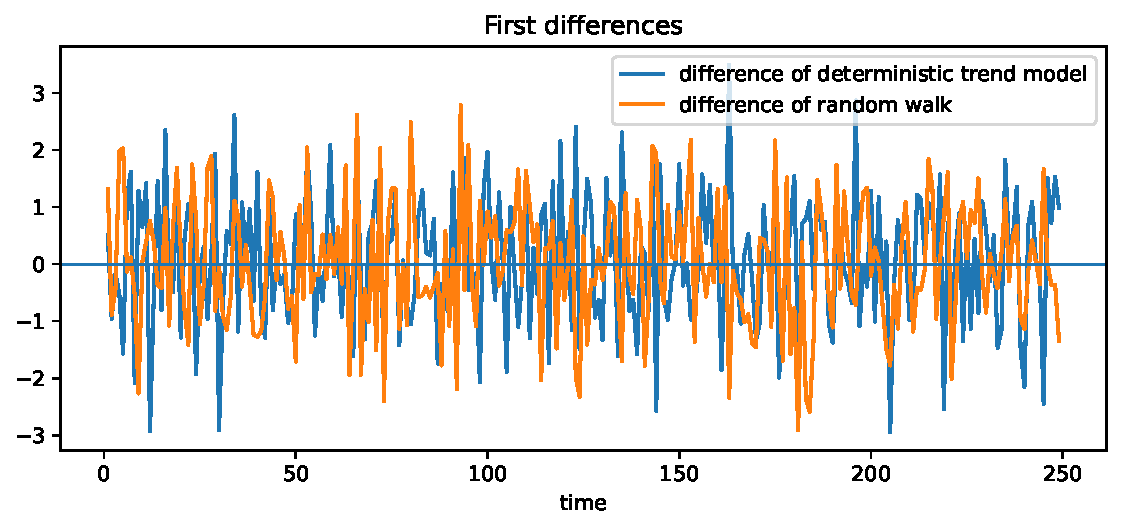
\includegraphics[keepaspectratio]{chapters/chapter-08-arima-differencing_files/figure-pdf/py-ch08-deterministic-vs-stochastic-trend-output-2.pdf}}

The first difference of the random walk is close to white noise with
drift. The first difference of the deterministic trend model is
stationary, but it has a different dependence structure from the
original stationary component.

\section{8.16 Python example: ACF before and after
differencing}\label{python-example-acf-before-and-after-differencing}

\protect\phantomsection\label{py-ch08-acf-before-after-differencing}
\begin{Shaded}
\begin{Highlighting}[]
\ImportTok{from}\NormalTok{ statsmodels.graphics.tsaplots }\ImportTok{import}\NormalTok{ plot\_acf, plot\_pacf}

\NormalTok{series }\OperatorTok{=}\NormalTok{ x\_rw}
\NormalTok{first\_difference }\OperatorTok{=}\NormalTok{ np.diff(series)}

\NormalTok{plot\_acf(series, lags}\OperatorTok{=}\DecValTok{40}\NormalTok{)}
\NormalTok{plt.title(}\StringTok{"ACF of original random walk with drift"}\NormalTok{)}
\NormalTok{plt.show()}

\NormalTok{plot\_acf(first\_difference, lags}\OperatorTok{=}\DecValTok{40}\NormalTok{)}
\NormalTok{plt.title(}\StringTok{"ACF after first differencing"}\NormalTok{)}
\NormalTok{plt.show()}

\NormalTok{plot\_pacf(first\_difference, lags}\OperatorTok{=}\DecValTok{40}\NormalTok{, method}\OperatorTok{=}\StringTok{"ywm"}\NormalTok{)}
\NormalTok{plt.title(}\StringTok{"PACF after first differencing"}\NormalTok{)}
\NormalTok{plt.show()}
\end{Highlighting}
\end{Shaded}

\begin{figure}[H]

{\centering \pandocbounded{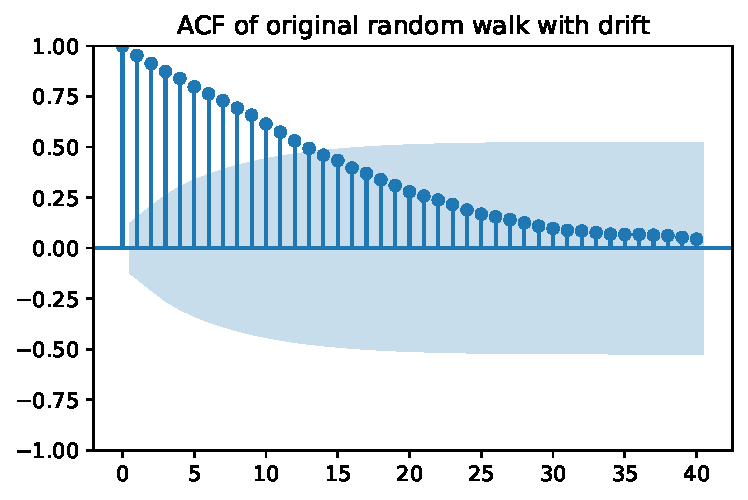
\includegraphics[keepaspectratio]{chapters/chapter-08-arima-differencing_files/figure-pdf/py-ch08-acf-before-after-differencing-output-1.pdf}}

}

\caption{ACF before and after differencing a nonstationary series.}

\end{figure}%

\pandocbounded{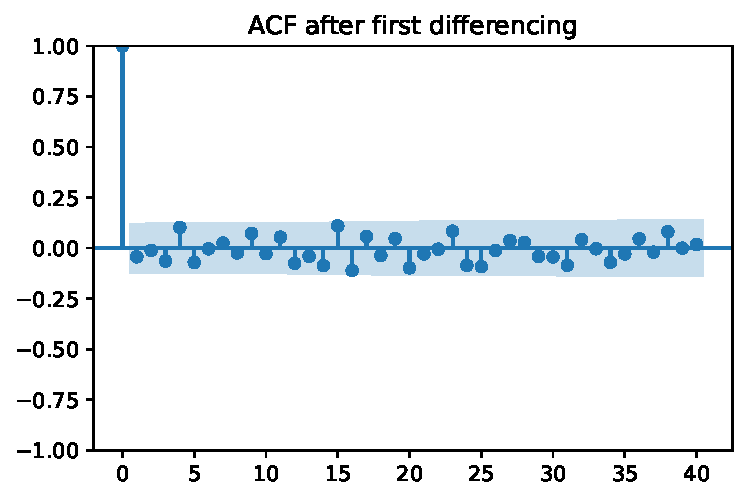
\includegraphics[keepaspectratio]{chapters/chapter-08-arima-differencing_files/figure-pdf/py-ch08-acf-before-after-differencing-output-2.pdf}}

\pandocbounded{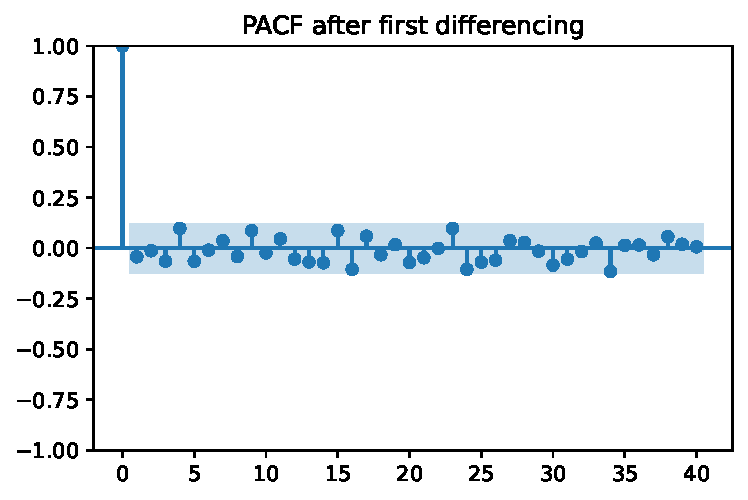
\includegraphics[keepaspectratio]{chapters/chapter-08-arima-differencing_files/figure-pdf/py-ch08-acf-before-after-differencing-output-3.pdf}}

The original random walk usually shows slow ACF decay. After
differencing, the ACF should be much closer to what we expect for a
stationary process.

\section{8.17 Python example: fitting ARIMA
models}\label{python-example-fitting-arima-models}

Here we simulate an ARIMA(\(1,1,1\)) series and fit several candidate
models.

\begin{Shaded}
\begin{Highlighting}[]
\ImportTok{import}\NormalTok{ warnings}
\ImportTok{import}\NormalTok{ pandas }\ImportTok{as}\NormalTok{ pd}
\ImportTok{from}\NormalTok{ statsmodels.tsa.arima.model }\ImportTok{import}\NormalTok{ ARIMA}

\NormalTok{warnings.filterwarnings(}\StringTok{"ignore"}\NormalTok{)}

\NormalTok{np.random.seed(}\DecValTok{2026}\NormalTok{)}

\NormalTok{n }\OperatorTok{=} \DecValTok{350}
\NormalTok{burn }\OperatorTok{=} \DecValTok{100}
\NormalTok{phi }\OperatorTok{=} \FloatTok{0.65}
\NormalTok{theta }\OperatorTok{=} \OperatorTok{{-}}\FloatTok{0.45}
\NormalTok{w }\OperatorTok{=}\NormalTok{ np.random.normal(size}\OperatorTok{=}\NormalTok{n }\OperatorTok{+}\NormalTok{ burn }\OperatorTok{+} \DecValTok{1}\NormalTok{)}
\NormalTok{y }\OperatorTok{=}\NormalTok{ np.zeros(n }\OperatorTok{+}\NormalTok{ burn }\OperatorTok{+} \DecValTok{1}\NormalTok{)}

\CommentTok{\# y\_t = phi y\_\{t{-}1\} + w\_t + theta w\_\{t{-}1\}}
\ControlFlowTok{for}\NormalTok{ i }\KeywordTok{in} \BuiltInTok{range}\NormalTok{(}\DecValTok{1}\NormalTok{, n }\OperatorTok{+}\NormalTok{ burn }\OperatorTok{+} \DecValTok{1}\NormalTok{):}
\NormalTok{    y[i] }\OperatorTok{=}\NormalTok{ phi }\OperatorTok{*}\NormalTok{ y[i}\OperatorTok{{-}}\DecValTok{1}\NormalTok{] }\OperatorTok{+}\NormalTok{ w[i] }\OperatorTok{+}\NormalTok{ theta }\OperatorTok{*}\NormalTok{ w[i}\OperatorTok{{-}}\DecValTok{1}\NormalTok{]}

\CommentTok{\# x\_t is integrated: difference x\_t is y\_t}
\NormalTok{x }\OperatorTok{=}\NormalTok{ np.cumsum(y)[burn:]}

\NormalTok{candidates }\OperatorTok{=}\NormalTok{ []}
\ControlFlowTok{for}\NormalTok{ p }\KeywordTok{in} \BuiltInTok{range}\NormalTok{(}\DecValTok{3}\NormalTok{):}
    \ControlFlowTok{for}\NormalTok{ d }\KeywordTok{in}\NormalTok{ [}\DecValTok{0}\NormalTok{, }\DecValTok{1}\NormalTok{, }\DecValTok{2}\NormalTok{]:}
        \ControlFlowTok{for}\NormalTok{ q }\KeywordTok{in} \BuiltInTok{range}\NormalTok{(}\DecValTok{3}\NormalTok{):}
            \ControlFlowTok{if}\NormalTok{ p }\OperatorTok{==} \DecValTok{0} \KeywordTok{and}\NormalTok{ d }\OperatorTok{==} \DecValTok{0} \KeywordTok{and}\NormalTok{ q }\OperatorTok{==} \DecValTok{0}\NormalTok{:}
                \ControlFlowTok{continue}
            \ControlFlowTok{try}\NormalTok{:}
\NormalTok{                fit }\OperatorTok{=}\NormalTok{ ARIMA(x, order}\OperatorTok{=}\NormalTok{(p, d, q), trend}\OperatorTok{=}\StringTok{"n"}\NormalTok{).fit()}
\NormalTok{                candidates.append(\{}
                    \StringTok{"p"}\NormalTok{: p,}
                    \StringTok{"d"}\NormalTok{: d,}
                    \StringTok{"q"}\NormalTok{: q,}
                    \StringTok{"AIC"}\NormalTok{: fit.aic,}
                    \StringTok{"BIC"}\NormalTok{: fit.bic}
\NormalTok{                \})}
            \ControlFlowTok{except} \PreprocessorTok{Exception}\NormalTok{:}
                \ControlFlowTok{pass}

\NormalTok{arima\_table }\OperatorTok{=}\NormalTok{ pd.DataFrame(candidates).sort\_values(}\StringTok{"AIC"}\NormalTok{)}
\NormalTok{arima\_table.head(}\DecValTok{10}\NormalTok{)}
\end{Highlighting}
\end{Shaded}

\protect\phantomsection\label{py-ch08-fit-arima-grid}
{\def\LTcaptype{none} % do not increment counter
\begin{longtable}[]{@{}llllll@{}}
\toprule\noalign{}
& p & d & q & AIC & BIC \\
\midrule\noalign{}
\endhead
\bottomrule\noalign{}
\endlastfoot
12 & 1 & 1 & 1 & 999.480986 & 1011.054786 \\
20 & 2 & 1 & 0 & 999.683095 & 1011.256894 \\
13 & 1 & 1 & 2 & 1000.970172 & 1016.401905 \\
21 & 2 & 1 & 1 & 1001.005003 & 1016.436736 \\
22 & 2 & 1 & 2 & 1001.125231 & 1020.414896 \\
16 & 1 & 2 & 2 & 1003.445706 & 1018.865994 \\
24 & 2 & 2 & 1 & 1003.616002 & 1019.036289 \\
4 & 0 & 1 & 2 & 1006.071812 & 1017.645611 \\
11 & 1 & 1 & 0 & 1006.441595 & 1014.157461 \\
15 & 1 & 2 & 1 & 1010.243564 & 1021.808780 \\
\end{longtable}
}

Fit the best candidate and inspect residuals.

\protect\phantomsection\label{py-ch08-arima-residuals}
\begin{Shaded}
\begin{Highlighting}[]
\ImportTok{from}\NormalTok{ statsmodels.stats.diagnostic }\ImportTok{import}\NormalTok{ acorr\_ljungbox}
\ImportTok{from}\NormalTok{ scipy }\ImportTok{import}\NormalTok{ stats}

\NormalTok{best }\OperatorTok{=}\NormalTok{ arima\_table.iloc[}\DecValTok{0}\NormalTok{]}
\NormalTok{best\_order }\OperatorTok{=}\NormalTok{ (}\BuiltInTok{int}\NormalTok{(best.p), }\BuiltInTok{int}\NormalTok{(best.d), }\BuiltInTok{int}\NormalTok{(best.q))}
\NormalTok{best\_fit }\OperatorTok{=}\NormalTok{ ARIMA(x, order}\OperatorTok{=}\NormalTok{best\_order, trend}\OperatorTok{=}\StringTok{"n"}\NormalTok{).fit()}
\NormalTok{resid }\OperatorTok{=}\NormalTok{ np.asarray(best\_fit.resid)}

\BuiltInTok{print}\NormalTok{(}\StringTok{"Selected order:"}\NormalTok{, best\_order)}
\BuiltInTok{print}\NormalTok{(acorr\_ljungbox(resid, lags}\OperatorTok{=}\NormalTok{[}\DecValTok{10}\NormalTok{, }\DecValTok{20}\NormalTok{], return\_df}\OperatorTok{=}\VariableTok{True}\NormalTok{))}

\NormalTok{fig, ax }\OperatorTok{=}\NormalTok{ plt.subplots(figsize}\OperatorTok{=}\NormalTok{(}\DecValTok{9}\NormalTok{, }\DecValTok{3}\NormalTok{))}
\NormalTok{ax.plot(resid)}
\NormalTok{ax.axhline(}\DecValTok{0}\NormalTok{, linewidth}\OperatorTok{=}\DecValTok{1}\NormalTok{)}
\NormalTok{ax.set\_title(}\StringTok{"ARIMA residuals"}\NormalTok{)}
\NormalTok{ax.set\_xlabel(}\StringTok{"time"}\NormalTok{)}
\NormalTok{plt.show()}

\NormalTok{plot\_acf(resid, lags}\OperatorTok{=}\DecValTok{30}\NormalTok{)}
\NormalTok{plt.title(}\StringTok{"Residual ACF"}\NormalTok{)}
\NormalTok{plt.show()}

\NormalTok{fig, ax }\OperatorTok{=}\NormalTok{ plt.subplots(figsize}\OperatorTok{=}\NormalTok{(}\DecValTok{5}\NormalTok{, }\DecValTok{5}\NormalTok{))}
\NormalTok{stats.probplot(resid, dist}\OperatorTok{=}\StringTok{"norm"}\NormalTok{, plot}\OperatorTok{=}\NormalTok{ax)}
\NormalTok{ax.set\_title(}\StringTok{"Residual Q{-}Q plot"}\NormalTok{)}
\NormalTok{plt.show()}
\end{Highlighting}
\end{Shaded}

\begin{verbatim}
Selected order: (1, 1, 1)
      lb_stat  lb_pvalue
10  16.463088   0.087121
20  20.349739   0.436252
\end{verbatim}

\begin{figure}[H]

{\centering \pandocbounded{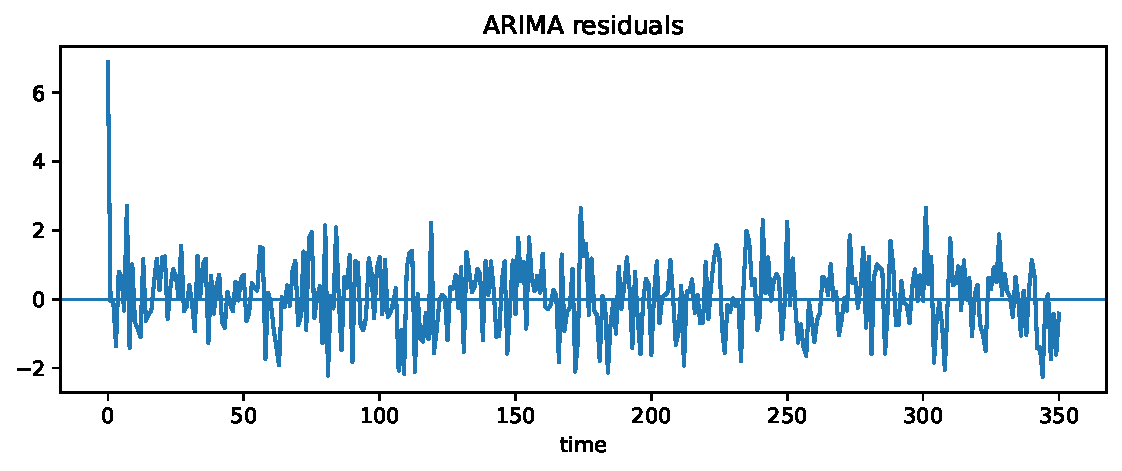
\includegraphics[keepaspectratio]{chapters/chapter-08-arima-differencing_files/figure-pdf/py-ch08-arima-residuals-output-2.pdf}}

}

\caption{Residual diagnostics for an ARIMA model.}

\end{figure}%

\pandocbounded{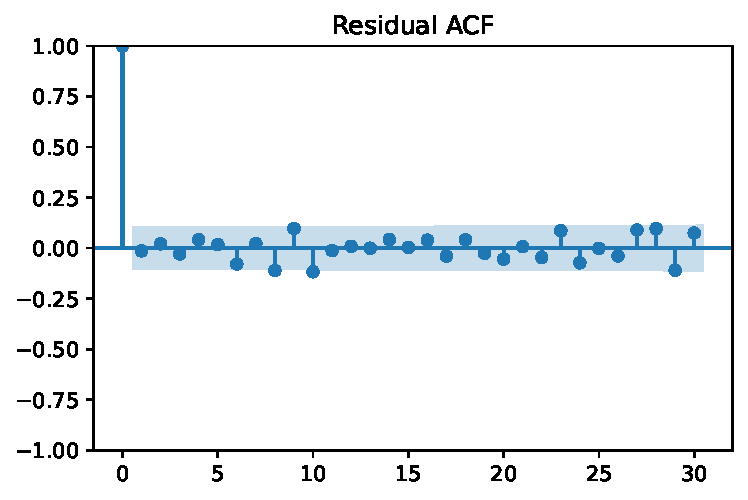
\includegraphics[keepaspectratio]{chapters/chapter-08-arima-differencing_files/figure-pdf/py-ch08-arima-residuals-output-3.pdf}}

\pandocbounded{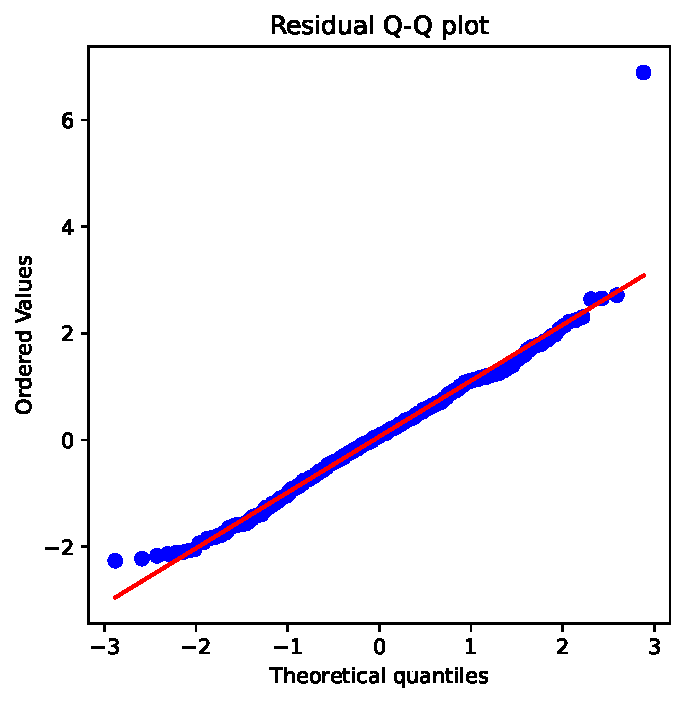
\includegraphics[keepaspectratio]{chapters/chapter-08-arima-differencing_files/figure-pdf/py-ch08-arima-residuals-output-4.pdf}}

\section{8.18 Python example: forecasting on the original
scale}\label{python-example-forecasting-on-the-original-scale}

The next example fits an ARIMA model and produces forecasts. Notice that
\texttt{statsmodels} automatically returns forecasts on the original
scale of \(X_t\), not on the differenced scale.

\begin{Shaded}
\begin{Highlighting}[]
\NormalTok{h }\OperatorTok{=} \DecValTok{40}
\NormalTok{fit }\OperatorTok{=}\NormalTok{ ARIMA(x, order}\OperatorTok{=}\NormalTok{best\_order, trend}\OperatorTok{=}\StringTok{"n"}\NormalTok{).fit()}
\NormalTok{forecast\_result }\OperatorTok{=}\NormalTok{ fit.get\_forecast(steps}\OperatorTok{=}\NormalTok{h)}
\NormalTok{forecast\_mean }\OperatorTok{=}\NormalTok{ forecast\_result.predicted\_mean}
\NormalTok{forecast\_ci }\OperatorTok{=}\NormalTok{ forecast\_result.conf\_int()}

\NormalTok{future\_index }\OperatorTok{=}\NormalTok{ np.arange(}\BuiltInTok{len}\NormalTok{(x), }\BuiltInTok{len}\NormalTok{(x) }\OperatorTok{+}\NormalTok{ h)}

\NormalTok{fig, ax }\OperatorTok{=}\NormalTok{ plt.subplots(figsize}\OperatorTok{=}\NormalTok{(}\DecValTok{9}\NormalTok{, }\DecValTok{4}\NormalTok{))}
\NormalTok{ax.plot(np.arange(}\BuiltInTok{len}\NormalTok{(x)), x, label}\OperatorTok{=}\StringTok{"observed"}\NormalTok{)}
\NormalTok{ax.plot(future\_index, forecast\_mean, label}\OperatorTok{=}\StringTok{"forecast"}\NormalTok{)}
\NormalTok{ax.fill\_between(}
\NormalTok{    future\_index,}
\NormalTok{    forecast\_ci[:, }\DecValTok{0}\NormalTok{],}
\NormalTok{    forecast\_ci[:, }\DecValTok{1}\NormalTok{],}
\NormalTok{    alpha}\OperatorTok{=}\FloatTok{0.25}\NormalTok{,}
\NormalTok{    label}\OperatorTok{=}\StringTok{"95}\SpecialCharTok{\% i}\StringTok{nterval"}
\NormalTok{)}
\NormalTok{ax.set\_title(}\SpecialStringTok{f"Forecast from ARIMA}\SpecialCharTok{\{}\NormalTok{best\_order}\SpecialCharTok{\}}\SpecialStringTok{"}\NormalTok{)}
\NormalTok{ax.set\_xlabel(}\StringTok{"time"}\NormalTok{)}
\NormalTok{ax.legend()}
\NormalTok{plt.show()}
\end{Highlighting}
\end{Shaded}

\begin{figure}[H]

{\centering \pandocbounded{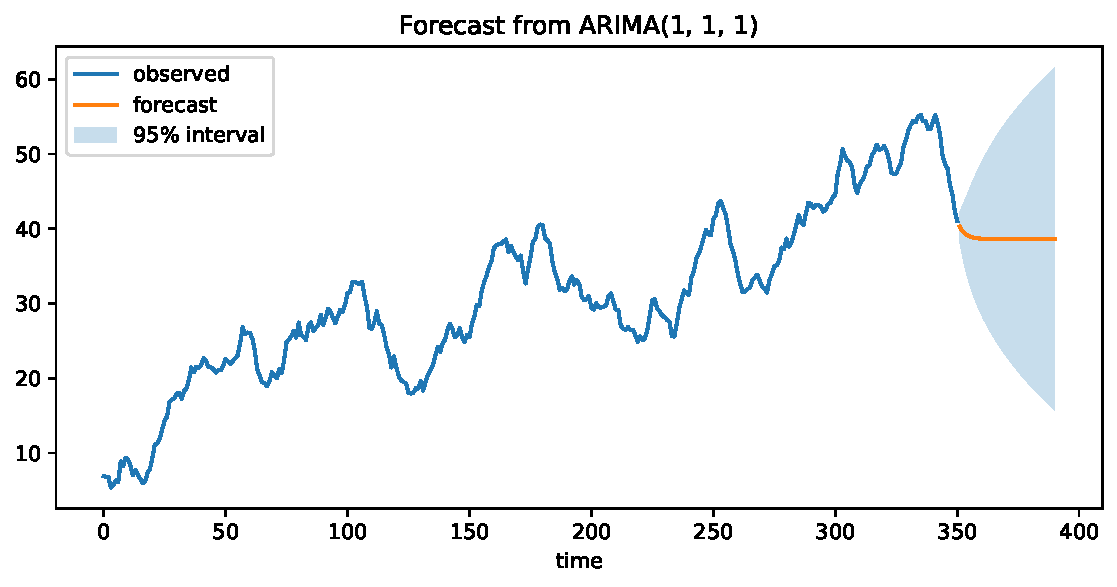
\includegraphics[keepaspectratio]{chapters/chapter-08-arima-differencing_files/figure-pdf/py-ch08-arima-forecast-output-1.pdf}}

}

\caption{ARIMA forecasts and forecast intervals on the original scale.}

\end{figure}%

Forecast intervals typically widen as the horizon increases because
future innovations accumulate through the integrated structure.

\section{8.19 AI-assisted study: asking useful
questions}\label{ai-assisted-study-asking-useful-questions}

AI tools can be helpful for explaining diagnostics, debugging code, and
generating model alternatives. They are not a replacement for checking
stationarity, residuals, and validation.

Good prompts:

\begin{quote}
I have a time series whose ACF decays slowly. Explain why this may
indicate a unit root or trend. Give me a checklist for deciding whether
to difference, detrend, or transform the data.
\end{quote}

\begin{quote}
Here is my ARIMA modeling workflow: {[}paste workflow{]}. Identify
possible data leakage, over-differencing, and missing residual
diagnostics. Do not choose a model only by AIC.
\end{quote}

\begin{quote}
I fit ARIMA(\(0,1,1\)). Explain how the model is written with the
backshift operator, and explain how forecasts on the differenced scale
are converted back to the original scale.
\end{quote}

\begin{quote}
My first-differenced series has a large negative lag-1 ACF. Give
possible mathematical explanations and how I should test whether I
over-differenced.
\end{quote}

Poor prompts:

\begin{quote}
What is the best ARIMA model for this data?
\end{quote}

\begin{quote}
Make the data stationary and forecast it.
\end{quote}

\begin{quote}
The AIC is smallest for ARIMA(\(2,2,2\)). Is this definitely the best
model?
\end{quote}

\begin{tcolorbox}[enhanced jigsaw, arc=.35mm, bottomrule=.15mm, bottomtitle=1mm, breakable, colback=white, colbacktitle=quarto-callout-warning-color!10!white, colframe=quarto-callout-warning-color-frame, coltitle=black, left=2mm, leftrule=.75mm, opacityback=0, opacitybacktitle=0.6, rightrule=.15mm, title=\textcolor{quarto-callout-warning-color}{\faExclamationTriangle}\hspace{0.5em}{AI verification rule}, titlerule=0mm, toprule=.15mm, toptitle=1mm]

When using AI for ARIMA modeling, always verify three things yourself:
the differencing order, residual whiteness, and out-of-sample forecast
performance.

\end{tcolorbox}

\section{8.20 Common mistakes}\label{common-mistakes-7}

\begin{enumerate}
\def\labelenumi{\arabic{enumi}.}
\item
  \textbf{Fitting ARMA directly to a nonstationary series.}\\
  This often leads to spurious dependence and unreliable forecasts.
\item
  \textbf{Differencing before looking at the data.}\\
  The time plot, variance behavior, and domain meaning should be
  considered first.
\item
  \textbf{Using \(d=2\) too quickly.}\\
  Second differencing can create unnecessary complexity and unstable
  forecasts.
\item
  \textbf{Ignoring transformations.}\\
  If variability increases with the level, a log or Box--Cox
  transformation may be needed before differencing.
\item
  \textbf{Choosing \(p,d,q\) only by AIC.}\\
  AIC should be combined with diagnostics and forecasting validation.
\item
  \textbf{Interpreting differenced forecasts incorrectly.}\\
  Forecasts of \(\nabla X_t\) must be accumulated to recover forecasts
  of \(X_t\).
\item
  \textbf{Forgetting constants and drift.}\\
  A constant in a differenced model has a different meaning from a mean
  in a stationary model.
\item
  \textbf{Ignoring outliers and structural breaks.}\\
  A single level shift can look like nonstationarity and mislead
  differencing decisions.
\end{enumerate}

\section{8.21 Exercises}\label{exercises-7}

\subsection{Conceptual exercises}\label{conceptual-exercises-6}

\begin{enumerate}
\def\labelenumi{\arabic{enumi}.}
\item
  Define ARIMA(\(p,d,q\)). Explain why ARMA(\(p,q\)) is a special case.
\item
  Show that a random walk \(X_t=X_{t-1}+W_t\) is ARIMA(\(0,1,0\)).
\item
  Suppose \(X_t=\beta_0+\beta_1t+W_t\), where \(W_t\) is white noise.
  Compute \(\nabla X_t\) and describe its autocorrelation structure.
\item
  Explain why over-differencing can produce negative autocorrelation at
  lag 1.
\item
  What is the difference between deterministic trend and stochastic
  trend? Give one example of each.
\item
  Explain why \(d\) should be chosen before \(p\) and \(q\).
\item
  Why do forecast intervals for integrated models usually widen as the
  forecast horizon grows?
\end{enumerate}

\subsection{Mathematical exercises}\label{mathematical-exercises-5}

\begin{enumerate}
\def\labelenumi{\arabic{enumi}.}
\setcounter{enumi}{7}
\item
  Compute \(\nabla^2X_t\) and \(\nabla^3X_t\) explicitly in terms of
  \(X_t,X_{t-1},\ldots\).
\item
  Let \(X_t=\delta+X_{t-1}+W_t\). Find \(E[X_t]\) and
  \(\operatorname{Var}(X_t)\) assuming \(X_0=0\).
\item
  Suppose \(\nabla X_t=\phi\nabla X_{t-1}+W_t\) with \(|\phi|<1\). Write
  the model as an ARIMA equation involving \(B\).
\item
  Suppose \(X_t\) is white noise. Let \(Y_t=\nabla X_t\). Compute
  \(\gamma_Y(0)\), \(\gamma_Y(1)\), and \(\rho_Y(1)\).
\item
  If \(Y_t=\nabla X_t\) is ARMA(\(1,1\)), write the full ARIMA model for
  \(X_t\) using \(\phi(B)\) and \(\theta(B)\).
\end{enumerate}

\subsection{Computational exercises}\label{computational-exercises-3}

\begin{enumerate}
\def\labelenumi{\arabic{enumi}.}
\setcounter{enumi}{12}
\item
  Simulate a random walk with drift. Plot the series, its first
  difference, and their ACFs.
\item
  Simulate an ARIMA(\(1,1,0\)) model. Fit ARIMA(\(0,1,0\)),
  ARIMA(\(1,1,0\)), and ARIMA(\(2,1,0\)). Compare AIC and residual
  diagnostics.
\item
  Take a real economic or environmental time series. Decide whether to
  log transform, difference, or detrend it. Justify your decision with
  plots and ACFs.
\item
  Use rolling-origin validation to compare ARIMA candidates. Report MAE,
  RMSE, and residual diagnostics.
\end{enumerate}

\section{8.22 Mini project: ARIMA modeling
report}\label{mini-project-arima-modeling-report}

Choose a real univariate time series with at least 100 observations.
Examples include monthly passengers, daily demand, weekly sales, stock
index levels, temperature anomalies, or ridership.

Your report should include:

\begin{enumerate}
\def\labelenumi{\arabic{enumi}.}
\tightlist
\item
  a description of the data and its time scale;
\item
  time plot and transformation decision;
\item
  differencing decision with explanation;
\item
  ACF/PACF of the stationary transformed series;
\item
  at least three fitted ARIMA candidates;
\item
  AIC/BIC comparison;
\item
  residual diagnostics;
\item
  forecast plot with intervals;
\item
  a paragraph explaining what AI assistance was used and how you
  verified it.
\end{enumerate}

\section{8.23 Chapter checklist}\label{chapter-checklist-5}

By the end of this chapter, you should be able to say:

\begin{itemize}
\tightlist
\item
  I can write \(\nabla X_t\) and \(\nabla^2X_t\) using the backshift
  operator.
\item
  I can explain why a random walk is nonstationary but its first
  difference is stationary.
\item
  I can define ARIMA(\(p,d,q\)) mathematically.
\item
  I can distinguish deterministic trend from stochastic trend.
\item
  I can use plots and ACF behavior to choose a preliminary \(d\).
\item
  I can recognize signs of over-differencing.
\item
  I can use ACF/PACF of \(\nabla^dX_t\) to propose \(p\) and \(q\).
\item
  I can fit ARIMA models in Python and check residuals.
\item
  I can explain how differenced forecasts are converted back to the
  original scale.
\item
  I can use AI tools for critique and explanation while verifying all
  modeling decisions.
\end{itemize}

\chapter{Seasonal ARIMA and Multiple
Seasonality}\label{seasonal-arima-and-multiple-seasonality}

\textbf{Part III. Nonstationary and Seasonal Models}\\
\textbf{Chapter goal:} learn how to model time series with repeating
seasonal structure. We develop seasonal lag operators, seasonal
differencing, pure seasonal ARMA models, multiplicative SARIMA models,
model-identification rules, diagnostics, backtesting,
multiple-seasonality extensions, and AI-assisted checks for seasonal
forecasting workflows.

\section{Learning objectives}\label{learning-objectives-8}

After studying this chapter, you should be able to:

\begin{enumerate}
\def\labelenumi{\arabic{enumi}.}
\tightlist
\item
  explain why ordinary ARIMA models are often insufficient for monthly,
  weekly, daily, hourly, or other seasonal data;
\item
  use the seasonal backshift operator \(B^s\) and the seasonal
  difference operator \(\nabla_s=1-B^s\);
\item
  define pure seasonal ARMA\((P,Q)_s\) models and full
  SARIMA\((p,d,q)(P,D,Q)_s\) models;
\item
  distinguish nonseasonal differencing from seasonal differencing;
\item
  recognize seasonal ACF and PACF patterns;
\item
  write and interpret multiplicative seasonal ARMA/SARIMA equations;
\item
  compare SARIMA forecasts with seasonal naive baselines;
\item
  diagnose SARIMA residuals using time plots, ACF, Ljung--Box tests, and
  backtesting;
\item
  understand why multiple seasonality often needs Fourier features,
  dynamic regression, Prophet-type models, or deep sequence models;
\item
  use AI tools to critique seasonal model choices while verifying all
  mathematical and empirical claims.
\end{enumerate}

\section{9.1 Why seasonality needs special
structure}\label{why-seasonality-needs-special-structure}

A nonseasonal ARIMA model explains dependence through recent values such
as \(X_{t-1}\), \(X_{t-2}\), and recent shocks such as \(W_{t-1}\),
\(W_{t-2}\). This is useful when the most relevant past values are
nearby in time.

Many real time series also depend strongly on values from the
\textbf{same season} in previous cycles:

\begin{itemize}
\tightlist
\item
  monthly airline passengers often depend on the same month last year;
\item
  daily retail demand often depends on the same day of the week;
\item
  hourly electricity demand often depends on the same hour yesterday and
  the same hour last week;
\item
  hospital admissions, web traffic, ride sharing, call centers, and
  financial volume all have calendar effects.
\end{itemize}

If the seasonal period is \(s\), then the seasonal lag is \(s\). For
monthly data with yearly seasonality, \(s=12\). For quarterly data with
yearly seasonality, \(s=4\). For daily data with weekly seasonality,
\(s=7\). For hourly data with daily seasonality, \(s=24\).

The simplest seasonal dependence says:

\[
X_t \text{ is related not only to } X_{t-1}, \text{ but also to } X_{t-s}.
\]

Ordinary ARIMA can technically include lag \(s\) by using a high-order
AR or MA model, but doing so directly is inefficient. Seasonal ARIMA
builds the lag \(s\) structure into the model.

\begin{tcolorbox}[enhanced jigsaw, arc=.35mm, bottomrule=.15mm, bottomtitle=1mm, breakable, colback=white, colbacktitle=quarto-callout-note-color!10!white, colframe=quarto-callout-note-color-frame, coltitle=black, left=2mm, leftrule=.75mm, opacityback=0, opacitybacktitle=0.6, rightrule=.15mm, title=\textcolor{quarto-callout-note-color}{\faInfo}\hspace{0.5em}{Core idea}, titlerule=0mm, toprule=.15mm, toptitle=1mm]

Seasonal models treat \(B^s\) as a basic operator, just as nonseasonal
ARIMA treats \(B\) as a basic operator.

\end{tcolorbox}

\section{9.2 The seasonal backshift
operator}\label{the-seasonal-backshift-operator}

The ordinary backshift operator is

\[
BX_t=X_{t-1}.
\]

The seasonal backshift operator is

\[
B^sX_t=X_{t-s}.
\]

For example, if \(s=12\), then

\[
B^{12}X_t=X_{t-12},
\]

which is the observation from the same month one year earlier.

The seasonal first-difference operator is

\[
\nabla_sX_t=X_t-X_{t-s}=(1-B^s)X_t.
\]

The \(D\)-th seasonal difference is

\[
\nabla_s^D X_t=(1-B^s)^D X_t.
\]

For \(D=2\),

\[
\nabla_s^2X_t=(1-B^s)^2X_t=X_t-2X_{t-s}+X_{t-2s}.
\]

In practice, seasonal differencing order \(D\) is usually \(0\) or
\(1\). Using \(D>1\) is uncommon and should require strong evidence.

\begin{tcolorbox}[enhanced jigsaw, arc=.35mm, bottomrule=.15mm, bottomtitle=1mm, breakable, colback=white, colbacktitle=quarto-callout-warning-color!10!white, colframe=quarto-callout-warning-color-frame, coltitle=black, left=2mm, leftrule=.75mm, opacityback=0, opacitybacktitle=0.6, rightrule=.15mm, title=\textcolor{quarto-callout-warning-color}{\faExclamationTriangle}\hspace{0.5em}{Seasonal differencing is not seasonal adjustment}, titlerule=0mm, toprule=.15mm, toptitle=1mm]

Seasonal differencing removes repeated stochastic seasonal level
changes, but it also changes the dependence structure. It is not the
same as estimating and subtracting deterministic seasonal means or
calendar effects.

\end{tcolorbox}

\section{9.3 Deterministic seasonality versus stochastic
seasonality}\label{deterministic-seasonality-versus-stochastic-seasonality}

Seasonality can enter a time series in more than one way.

\subsection{Deterministic seasonal
mean}\label{deterministic-seasonal-mean}

A simple deterministic seasonal model is

\[
X_t=m_{r(t)}+Y_t,
\]

where \(Y_t\) is stationary and \(m_{r(t)}\) is a repeating seasonal
mean. Here \(r(t)\) is the season index. For monthly data, \(r(t)\)
might be January, February, \(\ldots\), December.

If \(m_{r(t)}=m_{r(t-s)}\), then

\[
\nabla_sX_t=X_t-X_{t-s}=Y_t-Y_{t-s}.
\]

The seasonal mean disappears, but the stationary component has been
changed from \(Y_t\) to \(Y_t-Y_{t-s}\).

Alternatively, we could model the deterministic seasonal mean directly
using seasonal dummy variables or Fourier features:

\[
X_t=\beta_0+\sum_{j=1}^{s-1}\beta_jD_{j,t}+Y_t,
\]

where \(D_{j,t}\) indicates season \(j\).

\subsection{Stochastic seasonal trend}\label{stochastic-seasonal-trend}

A stochastic seasonal model is one in which the seasonal level evolves
randomly. The simplest example is the \textbf{seasonal random walk}:

\[
X_t=X_{t-s}+W_t.
\]

Equivalently,

\[
(1-B^s)X_t=W_t.
\]

This is SARIMA\((0,0,0)(0,1,0)_s\). Its best one-step forecast is close
to the value observed one full season ago.

\begin{tcolorbox}[enhanced jigsaw, arc=.35mm, bottomrule=.15mm, bottomtitle=1mm, breakable, colback=white, colbacktitle=quarto-callout-tip-color!10!white, colframe=quarto-callout-tip-color-frame, coltitle=black, left=2mm, leftrule=.75mm, opacityback=0, opacitybacktitle=0.6, rightrule=.15mm, title=\textcolor{quarto-callout-tip-color}{\faLightbulb}\hspace{0.5em}{Interpretation}, titlerule=0mm, toprule=.15mm, toptitle=1mm]

Deterministic seasonality says seasonal patterns repeat in a fixed way.
Stochastic seasonality says each season's level can evolve from cycle to
cycle.

\end{tcolorbox}

\section{9.4 Pure seasonal ARMA models}\label{pure-seasonal-arma-models}

A pure seasonal autoregressive moving-average model uses only seasonal
lags.

A pure seasonal ARMA\((P,Q)_s\) model is

\[
\Phi_P(B^s)X_t=\Theta_Q(B^s)W_t,
\]

where

\[
\Phi_P(B^s)=1-\Phi_1B^s-\Phi_2B^{2s}-\cdots-\Phi_PB^{Ps},
\]

and

\[
\Theta_Q(B^s)=1+\Theta_1B^s+\Theta_2B^{2s}+\cdots+\Theta_QB^{Qs}.
\]

For example, a pure seasonal ARMA\((1,1)_{12}\) model is

\[
(1-\Phi_1B^{12})X_t=(1+\Theta_1B^{12})W_t.
\]

In ordinary time notation,

\[
X_t=\Phi_1X_{t-12}+W_t+\Theta_1W_{t-12}.
\]

This model says that this month's deviation depends on the deviation
from the same month last year and on the shock from the same month last
year.

\section{9.5 Stationarity and invertibility for pure seasonal
models}\label{stationarity-and-invertibility-for-pure-seasonal-models}

The pure seasonal AR polynomial is

\[
\Phi_P(z^s)=1-\Phi_1z^s-\cdots-\Phi_Pz^{Ps}.
\]

The pure seasonal ARMA process is causal if the roots of
\(\Phi_P(z^s)=0\) lie outside the unit circle. It is invertible if the
roots of

\[
\Theta_Q(z^s)=1+\Theta_1z^s+\cdots+\Theta_Qz^{Qs}
\]

lie outside the unit circle.

For a pure seasonal AR\((1)_s\) model,

\[
X_t=\Phi X_{t-s}+W_t,
\]

causality requires

\[
|\Phi|<1.
\]

Then the causal expansion is

\[
X_t=W_t+\Phi W_{t-s}+\Phi^2W_{t-2s}+\cdots.
\]

The autocorrelation is nonzero at seasonal lags:

\[
\rho(ks)=\Phi^{|k|},\qquad k=0,1,2,\ldots,
\]

and equals zero at many nonseasonal lags when the model is purely
seasonal.

\section{9.6 Full multiplicative SARIMA
models}\label{full-multiplicative-sarima-models}

The most common seasonal ARIMA model combines nonseasonal and seasonal
factors multiplicatively.

A SARIMA\((p,d,q)(P,D,Q)_s\) model satisfies

\[
\phi_p(B)\Phi_P(B^s)(1-B)^d(1-B^s)^DX_t
=
\alpha+\theta_q(B)\Theta_Q(B^s)W_t.
\]

Here

\[
\phi_p(B)=1-\phi_1B-\cdots-\phi_pB^p,
\]

\[
\theta_q(B)=1+\theta_1B+\cdots+\theta_qB^q,
\]

\[
\Phi_P(B^s)=1-\Phi_1B^s-\cdots-\Phi_PB^{Ps},
\]

and

\[
\Theta_Q(B^s)=1+\Theta_1B^s+\cdots+\Theta_QB^{Qs}.
\]

The notation means:

{\def\LTcaptype{none} % do not increment counter
\begin{longtable}[]{@{}ll@{}}
\toprule\noalign{}
Symbol & Meaning \\
\midrule\noalign{}
\endhead
\bottomrule\noalign{}
\endlastfoot
\(p\) & nonseasonal AR order \\
\(d\) & nonseasonal differencing order \\
\(q\) & nonseasonal MA order \\
\(P\) & seasonal AR order \\
\(D\) & seasonal differencing order \\
\(Q\) & seasonal MA order \\
\(s\) & seasonal period \\
\end{longtable}
}

\begin{tcolorbox}[enhanced jigsaw, arc=.35mm, bottomrule=.15mm, bottomtitle=1mm, breakable, colback=white, colbacktitle=quarto-callout-note-color!10!white, colframe=quarto-callout-note-color-frame, coltitle=black, left=2mm, leftrule=.75mm, opacityback=0, opacitybacktitle=0.6, rightrule=.15mm, title=\textcolor{quarto-callout-note-color}{\faInfo}\hspace{0.5em}{Model class}, titlerule=0mm, toprule=.15mm, toptitle=1mm]

ARIMA\((p,d,q)\) is the special case SARIMA\((p,d,q)(0,0,0)_s\). Pure
seasonal models are the special case SARIMA\((0,0,0)(P,D,Q)_s\).

\end{tcolorbox}

\section{9.7 What multiplicative means}\label{what-multiplicative-means}

Consider a simple multiplicative seasonal AR model:

\[
(1-\phi B)(1-\Phi B^s)X_t=W_t.
\]

Expanding the left-hand side gives

\[
(1-\phi B-\Phi B^s+\phi\Phi B^{s+1})X_t=W_t.
\]

Thus

\[
X_t=\phi X_{t-1}+\Phi X_{t-s}-\phi\Phi X_{t-s-1}+W_t.
\]

The multiplicative model is not merely an AR model with lags \(1\) and
\(s\). It also includes the interaction lag \(s+1\) with coefficient
\(-\phi\Phi\).

Similarly, for a multiplicative MA model,

\[
(1+\theta B)(1+\Theta B^s)W_t
=
W_t+\theta W_{t-1}+\Theta W_{t-s}+\theta\Theta W_{t-s-1}.
\]

The product structure gives a parsimonious model while still allowing
interaction between short-range and seasonal dependence.

\section{9.8 Seasonal differencing}\label{seasonal-differencing-1}

Seasonal differencing is often used when a series has a seasonal
stochastic trend. For example,

\[
X_t=X_{t-s}+W_t
\]

is not stationary, but

\[
\nabla_sX_t=X_t-X_{t-s}=W_t
\]

is stationary.

A model with both nonseasonal and seasonal differencing is

\[
Y_t=(1-B)^d(1-B^s)^DX_t.
\]

For \(d=1\) and \(D=1\),

\[
Y_t=(1-B)(1-B^s)X_t.
\]

Expanding,

\[
Y_t=X_t-X_{t-1}-X_{t-s}+X_{t-s-1}.
\]

This transformation removes both local trend and seasonal trend, but it
can be aggressive. It should be justified by plots, ACF behavior,
diagnostics, and validation.

\begin{tcolorbox}[enhanced jigsaw, arc=.35mm, bottomrule=.15mm, bottomtitle=1mm, breakable, colback=white, colbacktitle=quarto-callout-warning-color!10!white, colframe=quarto-callout-warning-color-frame, coltitle=black, left=2mm, leftrule=.75mm, opacityback=0, opacitybacktitle=0.6, rightrule=.15mm, title=\textcolor{quarto-callout-warning-color}{\faExclamationTriangle}\hspace{0.5em}{Avoid automatic double differencing}, titlerule=0mm, toprule=.15mm, toptitle=1mm]

Applying both \(d=1\) and \(D=1\) can be necessary, but it can also
over-difference the series. After differencing, always inspect the
transformed series and its ACF.

\end{tcolorbox}

\section{9.9 Seasonal ACF and PACF
patterns}\label{seasonal-acf-and-pacf-patterns}

The ACF and PACF for SARIMA models should be read at two scales:

\begin{enumerate}
\def\labelenumi{\arabic{enumi}.}
\tightlist
\item
  \textbf{short lags}: \(1,2,3,\ldots\);
\item
  \textbf{seasonal lags}: \(s,2s,3s,\ldots\).
\end{enumerate}

For a stationary transformed series \(Y_t=(1-B)^d(1-B^s)^DX_t\):

{\def\LTcaptype{none} % do not increment counter
\begin{longtable}[]{@{}
  >{\raggedright\arraybackslash}p{(\linewidth - 4\tabcolsep) * \real{0.3333}}
  >{\raggedright\arraybackslash}p{(\linewidth - 4\tabcolsep) * \real{0.3333}}
  >{\raggedright\arraybackslash}p{(\linewidth - 4\tabcolsep) * \real{0.3333}}@{}}
\toprule\noalign{}
\begin{minipage}[b]{\linewidth}\raggedright
Candidate seasonal component
\end{minipage} & \begin{minipage}[b]{\linewidth}\raggedright
ACF at seasonal lags
\end{minipage} & \begin{minipage}[b]{\linewidth}\raggedright
PACF at seasonal lags
\end{minipage} \\
\midrule\noalign{}
\endhead
\bottomrule\noalign{}
\endlastfoot
seasonal AR\((P)_s\) & decays at \(s,2s,3s,\ldots\) & cuts off after
\(Ps\) \\
seasonal MA\((Q)_s\) & cuts off after \(Qs\) & decays at
\(s,2s,3s,\ldots\) \\
seasonal ARMA\((P,Q)_s\) & decays & decays \\
\end{longtable}
}

Nonseasonal patterns are interpreted in the ordinary way:

{\def\LTcaptype{none} % do not increment counter
\begin{longtable}[]{@{}
  >{\raggedright\arraybackslash}p{(\linewidth - 4\tabcolsep) * \real{0.3333}}
  >{\raggedright\arraybackslash}p{(\linewidth - 4\tabcolsep) * \real{0.3333}}
  >{\raggedright\arraybackslash}p{(\linewidth - 4\tabcolsep) * \real{0.3333}}@{}}
\toprule\noalign{}
\begin{minipage}[b]{\linewidth}\raggedright
Candidate nonseasonal component
\end{minipage} & \begin{minipage}[b]{\linewidth}\raggedright
ACF at short lags
\end{minipage} & \begin{minipage}[b]{\linewidth}\raggedright
PACF at short lags
\end{minipage} \\
\midrule\noalign{}
\endhead
\bottomrule\noalign{}
\endlastfoot
AR(\(p\)) & decays & cuts off after \(p\) \\
MA(\(q\)) & cuts off after \(q\) & decays \\
ARMA(\(p,q\)) & decays & decays \\
\end{longtable}
}

A strong spike at lag \(s\) in the ACF often suggests a seasonal MA
component or seasonal differencing. A slowly decaying ACF at seasonal
lags suggests seasonal nonstationarity or a seasonal AR component.

\begin{tcolorbox}[enhanced jigsaw, arc=.35mm, bottomrule=.15mm, bottomtitle=1mm, breakable, colback=white, colbacktitle=quarto-callout-tip-color!10!white, colframe=quarto-callout-tip-color-frame, coltitle=black, left=2mm, leftrule=.75mm, opacityback=0, opacitybacktitle=0.6, rightrule=.15mm, title=\textcolor{quarto-callout-tip-color}{\faLightbulb}\hspace{0.5em}{Reading seasonal plots}, titlerule=0mm, toprule=.15mm, toptitle=1mm]

For monthly data, inspect lags \(12,24,36,\ldots\). For quarterly data,
inspect lags \(4,8,12,\ldots\). For daily weekly data, inspect lags
\(7,14,21,\ldots\).

\end{tcolorbox}

\section{9.10 A modeling workflow for
SARIMA}\label{a-modeling-workflow-for-sarima}

A practical SARIMA workflow is:

\begin{enumerate}
\def\labelenumi{\arabic{enumi}.}
\tightlist
\item
  \textbf{Plot the series.} Look for trend, seasonality, changing
  variance, outliers, and structural breaks.
\item
  \textbf{Identify the seasonal period \(s\).} Use domain knowledge
  first.
\item
  \textbf{Stabilize variance if needed.} Common choices include log
  transform or Box--Cox transform.
\item
  \textbf{Choose seasonal differencing \(D\).} If seasonal patterns
  drift or seasonal ACF decays slowly, try \(D=1\).
\item
  \textbf{Choose nonseasonal differencing \(d\).} If trend remains after
  seasonal differencing, try \(d=1\).
\item
  \textbf{Inspect ACF and PACF of the transformed series.} Propose small
  values of \(p,q,P,Q\).
\item
  \textbf{Fit several candidate models.} Use maximum likelihood or
  conditional likelihood.
\item
  \textbf{Check residuals.} Residuals should look like white noise.
\item
  \textbf{Compare forecasts by backtesting.} Do not rely only on AIC.
\item
  \textbf{Report a baseline comparison.} Seasonal naive is often a
  strong baseline.
\end{enumerate}

A typical starting grid for monthly data might be

\[
p,q,P,Q\in\{0,1,2\},\qquad d,D\in\{0,1\},\qquad s=12.
\]

Large grids are possible, but the goal is not to automate blindly. The
model should remain interpretable and diagnostically reasonable.

\section{9.11 Seasonal naive forecasts}\label{seasonal-naive-forecasts}

Before fitting SARIMA, always compare with a seasonal naive forecast.
For seasonal period \(s\), the seasonal naive \(h\)-step forecast uses
the most recent observation from the same season:

\[
\widehat X_{n+h|n}=X_{n+h-ms},
\]

where \(m\) is the smallest positive integer such that \(n+h-ms\le n\).

For monthly data, the forecast for next January is last January, the
forecast for next February is last February, and so on.

The seasonal naive method is simple, but for strongly seasonal data it
is often difficult to beat. A modern forecasting workflow should treat
it as a serious baseline.

\section{9.12 Forecasting with SARIMA}\label{forecasting-with-sarima}

A fitted SARIMA model forecasts the transformed stationary process and
then reconstructs forecasts on the original scale. If the model uses
seasonal differencing,

\[
Y_t=(1-B^s)X_t=X_t-X_{t-s},
\]

then

\[
X_t=Y_t+X_{t-s}.
\]

Thus future forecasts are recursively reconstructed using previous
seasonal values and forecasted seasonal differences.

If the model uses both ordinary and seasonal differencing,

\[
Y_t=(1-B)(1-B^s)X_t,
\]

then reconstruction requires reversing both operations. Software
performs this recursion automatically, but students should understand
that forecast intervals widen because future innovations accumulate
through the integration operations.

\section{9.13 Residual diagnostics}\label{residual-diagnostics-1}

After fitting a SARIMA model, residuals should behave like white noise.
Diagnostics include:

\begin{enumerate}
\def\labelenumi{\arabic{enumi}.}
\tightlist
\item
  \textbf{Time plot of residuals.} Look for changing variance, trend, or
  remaining seasonality.
\item
  \textbf{Residual ACF.} Seasonal spikes at \(s,2s,\ldots\) suggest
  missing seasonal structure.
\item
  \textbf{Ljung--Box test.} Test whether a group of autocorrelations is
  jointly significant.
\item
  \textbf{Q-Q plot.} Check whether Gaussian forecast intervals are
  reasonable.
\item
  \textbf{Backtesting.} Compare out-of-sample forecast errors with
  baseline models.
\end{enumerate}

If residuals still show seasonal autocorrelation, possible fixes
include:

\begin{itemize}
\tightlist
\item
  add a seasonal AR or seasonal MA term;
\item
  reconsider seasonal differencing \(D\);
\item
  add deterministic seasonal regressors;
\item
  transform the data;
\item
  model outliers or interventions;
\item
  consider multiple-seasonality models.
\end{itemize}

\section{9.14 Multiple seasonality}\label{multiple-seasonality}

A single SARIMA model is designed around one seasonal period \(s\). Many
modern applications have multiple seasonal periods.

Examples:

{\def\LTcaptype{none} % do not increment counter
\begin{longtable}[]{@{}
  >{\raggedright\arraybackslash}p{(\linewidth - 2\tabcolsep) * \real{0.5000}}
  >{\raggedright\arraybackslash}p{(\linewidth - 2\tabcolsep) * \real{0.5000}}@{}}
\toprule\noalign{}
\begin{minipage}[b]{\linewidth}\raggedright
Data frequency
\end{minipage} & \begin{minipage}[b]{\linewidth}\raggedright
Common seasonalities
\end{minipage} \\
\midrule\noalign{}
\endhead
\bottomrule\noalign{}
\endlastfoot
hourly electricity demand & daily \(s=24\), weekly \(s=168\), yearly
approximately \(8760\) \\
daily retail sales & weekly \(s=7\), yearly approximately \(365\) \\
minute-level web traffic & hourly, daily, weekly \\
hospital operations & day-of-week, holiday, annual cycles \\
\end{longtable}
}

A direct SARIMA model with several seasonal periods can become large,
unstable, and hard to estimate. In such settings, useful alternatives
include:

\begin{enumerate}
\def\labelenumi{\arabic{enumi}.}
\tightlist
\item
  deterministic Fourier features;
\item
  dynamic harmonic regression;
\item
  Prophet-type additive models;
\item
  TBATS-style exponential smoothing models;
\item
  machine-learning models with calendar and lag features;
\item
  deep sequence models such as TCNs, RNNs, LSTMs, and transformers.
\end{enumerate}

A Fourier seasonal regression with multiple periods has the form

\[
X_t
=
\beta_0
+
\sum_{m\in\mathcal S}\sum_{k=1}^{K_m}
\left[
 a_{k,m}\cos\left(\frac{2\pi kt}{m}\right)
+b_{k,m}\sin\left(\frac{2\pi kt}{m}\right)
\right]
+Y_t,
\]

where \(\mathcal S\) is the set of seasonal periods and \(Y_t\) is a
residual time-series process.

\begin{tcolorbox}[enhanced jigsaw, arc=.35mm, bottomrule=.15mm, bottomtitle=1mm, breakable, colback=white, colbacktitle=quarto-callout-note-color!10!white, colframe=quarto-callout-note-color-frame, coltitle=black, left=2mm, leftrule=.75mm, opacityback=0, opacitybacktitle=0.6, rightrule=.15mm, title=\textcolor{quarto-callout-note-color}{\faInfo}\hspace{0.5em}{Modern connection}, titlerule=0mm, toprule=.15mm, toptitle=1mm]

Classical SARIMA handles one dominant seasonal period well. Modern
forecasting systems often combine seasonal differencing, Fourier
features, calendar features, and flexible ML or deep learning models.

\end{tcolorbox}

\section{9.15 Calendar effects, holidays, and
interventions}\label{calendar-effects-holidays-and-interventions}

Seasonality is regular. Holidays and interventions are often irregular.

A holiday effect may be represented by a regression variable \(H_t\):

\[
X_t=\text{seasonal component}+\beta_HH_t+Y_t.
\]

Examples include Thanksgiving, Lunar New Year, school breaks, weather
emergencies, promotions, policy changes, product launches, and
pandemics.

A SARIMA model can be extended to SARIMAX by including exogenous
regressors:

\[
\phi(B)\Phi(B^s)(1-B)^d(1-B^s)^D
\left(X_t-\beta^\top z_t\right)
=
\theta(B)\Theta(B^s)W_t.
\]

Here \(z_t\) may contain calendar effects, weather variables, price
variables, holiday indicators, or intervention indicators.

The key modeling principle is that dependence and regression effects
should both be checked. If residuals remain autocorrelated after
regression, a time-series error model is needed.

\section{9.16 Interactive HTML: Seasonal differencing and SAR structure
explorer}\label{interactive-html-seasonal-differencing-and-sar-structure-explorer}

The interactive below simulates a series with trend, deterministic
seasonality, short-memory AR dependence, and seasonal AR dependence. Use
the controls to see how ordinary differencing and seasonal differencing
change the time plot and ACF.

\begin{tcolorbox}[enhanced jigsaw, arc=.35mm, bottomrule=.15mm, bottomtitle=1mm, breakable, colback=white, colbacktitle=quarto-callout-warning-color!10!white, colframe=quarto-callout-warning-color-frame, coltitle=black, left=2mm, leftrule=.75mm, opacityback=0, opacitybacktitle=0.6, rightrule=.15mm, title=\textcolor{quarto-callout-warning-color}{\faExclamationTriangle}\hspace{0.5em}{Plotly loading rule}, titlerule=0mm, toprule=.15mm, toptitle=1mm]

This chapter uses \texttt{Plotly.newPlot} but does not load Plotly.js.
The e-book package loads Plotly.js once globally through the shared
header file.

\end{tcolorbox}

\section{9.17 Python example: simulate seasonal
data}\label{python-example-simulate-seasonal-data}

The following example simulates a seasonal time series with a trend,
deterministic yearly seasonality, and seasonal autoregressive
dependence.

\begin{Shaded}
\begin{Highlighting}[]
\ImportTok{import}\NormalTok{ numpy }\ImportTok{as}\NormalTok{ np}
\ImportTok{import}\NormalTok{ pandas }\ImportTok{as}\NormalTok{ pd}
\ImportTok{import}\NormalTok{ matplotlib.pyplot }\ImportTok{as}\NormalTok{ plt}

\NormalTok{np.random.seed(}\DecValTok{7339}\NormalTok{)}

\NormalTok{n }\OperatorTok{=} \DecValTok{180}
\NormalTok{s }\OperatorTok{=} \DecValTok{12}
\NormalTok{phi }\OperatorTok{=} \FloatTok{0.35}
\NormalTok{Phi }\OperatorTok{=} \FloatTok{0.55}
\NormalTok{sigma }\OperatorTok{=} \FloatTok{1.0}

\NormalTok{time }\OperatorTok{=}\NormalTok{ np.arange(n)}
\NormalTok{noise }\OperatorTok{=}\NormalTok{ np.random.normal(scale}\OperatorTok{=}\NormalTok{sigma, size}\OperatorTok{=}\NormalTok{n)}
\NormalTok{y }\OperatorTok{=}\NormalTok{ np.zeros(n)}

\CommentTok{\# Multiplicative seasonal AR: (1 {-} phi B)(1 {-} Phi B\^{}s) y\_t = w\_t}
\ControlFlowTok{for}\NormalTok{ t }\KeywordTok{in} \BuiltInTok{range}\NormalTok{(n):}
\NormalTok{    y1 }\OperatorTok{=}\NormalTok{ y[t}\OperatorTok{{-}}\DecValTok{1}\NormalTok{] }\ControlFlowTok{if}\NormalTok{ t}\OperatorTok{{-}}\DecValTok{1} \OperatorTok{\textgreater{}=} \DecValTok{0} \ControlFlowTok{else} \DecValTok{0}
\NormalTok{    ys }\OperatorTok{=}\NormalTok{ y[t}\OperatorTok{{-}}\NormalTok{s] }\ControlFlowTok{if}\NormalTok{ t}\OperatorTok{{-}}\NormalTok{s }\OperatorTok{\textgreater{}=} \DecValTok{0} \ControlFlowTok{else} \DecValTok{0}
\NormalTok{    ysi }\OperatorTok{=}\NormalTok{ y[t}\OperatorTok{{-}}\NormalTok{s}\OperatorTok{{-}}\DecValTok{1}\NormalTok{] }\ControlFlowTok{if}\NormalTok{ t}\OperatorTok{{-}}\NormalTok{s}\OperatorTok{{-}}\DecValTok{1} \OperatorTok{\textgreater{}=} \DecValTok{0} \ControlFlowTok{else} \DecValTok{0}
\NormalTok{    y[t] }\OperatorTok{=}\NormalTok{ phi}\OperatorTok{*}\NormalTok{y1 }\OperatorTok{+}\NormalTok{ Phi}\OperatorTok{*}\NormalTok{ys }\OperatorTok{{-}}\NormalTok{ phi}\OperatorTok{*}\NormalTok{Phi}\OperatorTok{*}\NormalTok{ysi }\OperatorTok{+}\NormalTok{ noise[t]}

\NormalTok{seasonal\_mean }\OperatorTok{=} \DecValTok{4}\OperatorTok{*}\NormalTok{np.sin(}\DecValTok{2}\OperatorTok{*}\NormalTok{np.pi}\OperatorTok{*}\NormalTok{time}\OperatorTok{/}\NormalTok{s) }\OperatorTok{+} \FloatTok{1.5}\OperatorTok{*}\NormalTok{np.cos(}\DecValTok{4}\OperatorTok{*}\NormalTok{np.pi}\OperatorTok{*}\NormalTok{time}\OperatorTok{/}\NormalTok{s)}
\NormalTok{trend }\OperatorTok{=} \FloatTok{0.03}\OperatorTok{*}\NormalTok{time}
\NormalTok{x }\OperatorTok{=} \DecValTok{20} \OperatorTok{+}\NormalTok{ trend }\OperatorTok{+}\NormalTok{ seasonal\_mean }\OperatorTok{+}\NormalTok{ y}

\NormalTok{dates }\OperatorTok{=}\NormalTok{ pd.date\_range(}\StringTok{"2010{-}01{-}01"}\NormalTok{, periods}\OperatorTok{=}\NormalTok{n, freq}\OperatorTok{=}\StringTok{"MS"}\NormalTok{)}
\NormalTok{series }\OperatorTok{=}\NormalTok{ pd.Series(x, index}\OperatorTok{=}\NormalTok{dates, name}\OperatorTok{=}\StringTok{"x"}\NormalTok{)}

\NormalTok{fig, ax }\OperatorTok{=}\NormalTok{ plt.subplots(figsize}\OperatorTok{=}\NormalTok{(}\DecValTok{10}\NormalTok{, }\DecValTok{4}\NormalTok{))}
\NormalTok{series.plot(ax}\OperatorTok{=}\NormalTok{ax)}
\NormalTok{ax.set\_title(}\StringTok{"Simulated monthly seasonal time series"}\NormalTok{)}
\NormalTok{ax.set\_xlabel(}\StringTok{"date"}\NormalTok{)}
\NormalTok{ax.set\_ylabel(}\StringTok{"value"}\NormalTok{)}
\NormalTok{plt.show()}
\end{Highlighting}
\end{Shaded}

\pandocbounded{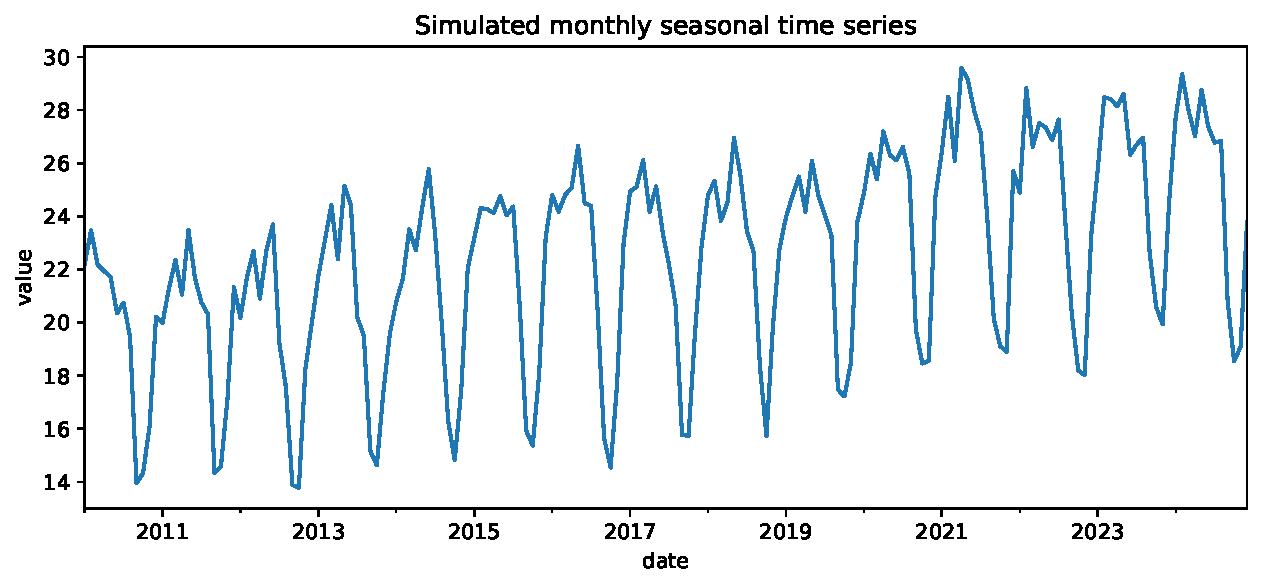
\includegraphics[keepaspectratio]{chapters/chapter-09-sarima-multiple-seasonality_files/figure-pdf/cell-2-output-1.pdf}}

\section{9.18 Python example: seasonal differencing and
ACF/PACF}\label{python-example-seasonal-differencing-and-acfpacf}

\begin{Shaded}
\begin{Highlighting}[]
\ImportTok{from}\NormalTok{ statsmodels.graphics.tsaplots }\ImportTok{import}\NormalTok{ plot\_acf, plot\_pacf}

\NormalTok{seasonally\_diff }\OperatorTok{=}\NormalTok{ series.diff(s).dropna()}
\NormalTok{both\_diff }\OperatorTok{=}\NormalTok{ seasonally\_diff.diff().dropna()}

\NormalTok{fig, axes }\OperatorTok{=}\NormalTok{ plt.subplots(}\DecValTok{3}\NormalTok{, }\DecValTok{1}\NormalTok{, figsize}\OperatorTok{=}\NormalTok{(}\DecValTok{10}\NormalTok{, }\DecValTok{8}\NormalTok{), sharex}\OperatorTok{=}\VariableTok{False}\NormalTok{)}
\NormalTok{series.plot(ax}\OperatorTok{=}\NormalTok{axes[}\DecValTok{0}\NormalTok{])}
\NormalTok{axes[}\DecValTok{0}\NormalTok{].set\_title(}\StringTok{"Original series"}\NormalTok{)}
\NormalTok{seasonally\_diff.plot(ax}\OperatorTok{=}\NormalTok{axes[}\DecValTok{1}\NormalTok{])}
\NormalTok{axes[}\DecValTok{1}\NormalTok{].set\_title(}\StringTok{"Seasonal difference: X\_t {-} X\_\{t{-}12\}"}\NormalTok{)}
\NormalTok{both\_diff.plot(ax}\OperatorTok{=}\NormalTok{axes[}\DecValTok{2}\NormalTok{])}
\NormalTok{axes[}\DecValTok{2}\NormalTok{].set\_title(}\StringTok{"Seasonal difference followed by ordinary difference"}\NormalTok{)}
\NormalTok{plt.tight\_layout()}
\NormalTok{plt.show()}

\NormalTok{fig, axes }\OperatorTok{=}\NormalTok{ plt.subplots(}\DecValTok{1}\NormalTok{, }\DecValTok{2}\NormalTok{, figsize}\OperatorTok{=}\NormalTok{(}\DecValTok{12}\NormalTok{, }\DecValTok{4}\NormalTok{))}
\NormalTok{plot\_acf(seasonally\_diff, lags}\OperatorTok{=}\DecValTok{48}\NormalTok{, ax}\OperatorTok{=}\NormalTok{axes[}\DecValTok{0}\NormalTok{])}
\NormalTok{axes[}\DecValTok{0}\NormalTok{].set\_title(}\StringTok{"ACF after seasonal differencing"}\NormalTok{)}
\NormalTok{plot\_pacf(seasonally\_diff, lags}\OperatorTok{=}\DecValTok{48}\NormalTok{, ax}\OperatorTok{=}\NormalTok{axes[}\DecValTok{1}\NormalTok{], method}\OperatorTok{=}\StringTok{"ywm"}\NormalTok{)}
\NormalTok{axes[}\DecValTok{1}\NormalTok{].set\_title(}\StringTok{"PACF after seasonal differencing"}\NormalTok{)}
\NormalTok{plt.tight\_layout()}
\NormalTok{plt.show()}
\end{Highlighting}
\end{Shaded}

\pandocbounded{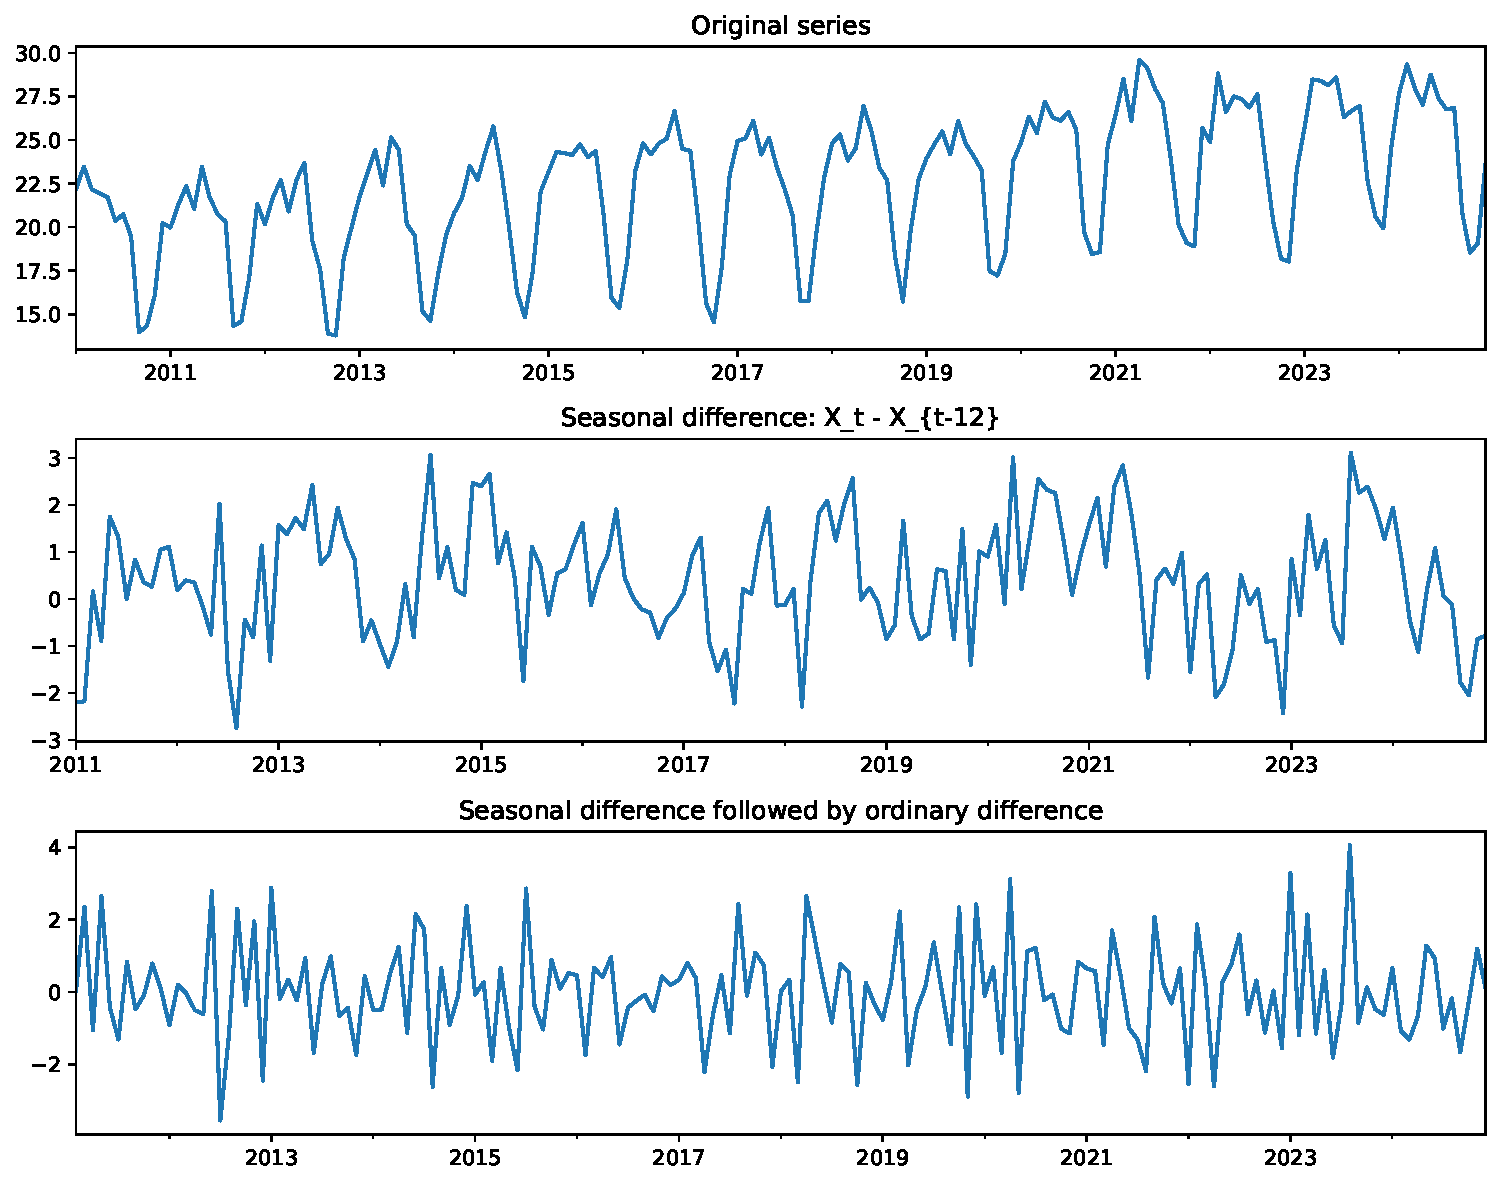
\includegraphics[keepaspectratio]{chapters/chapter-09-sarima-multiple-seasonality_files/figure-pdf/cell-3-output-1.pdf}}

\pandocbounded{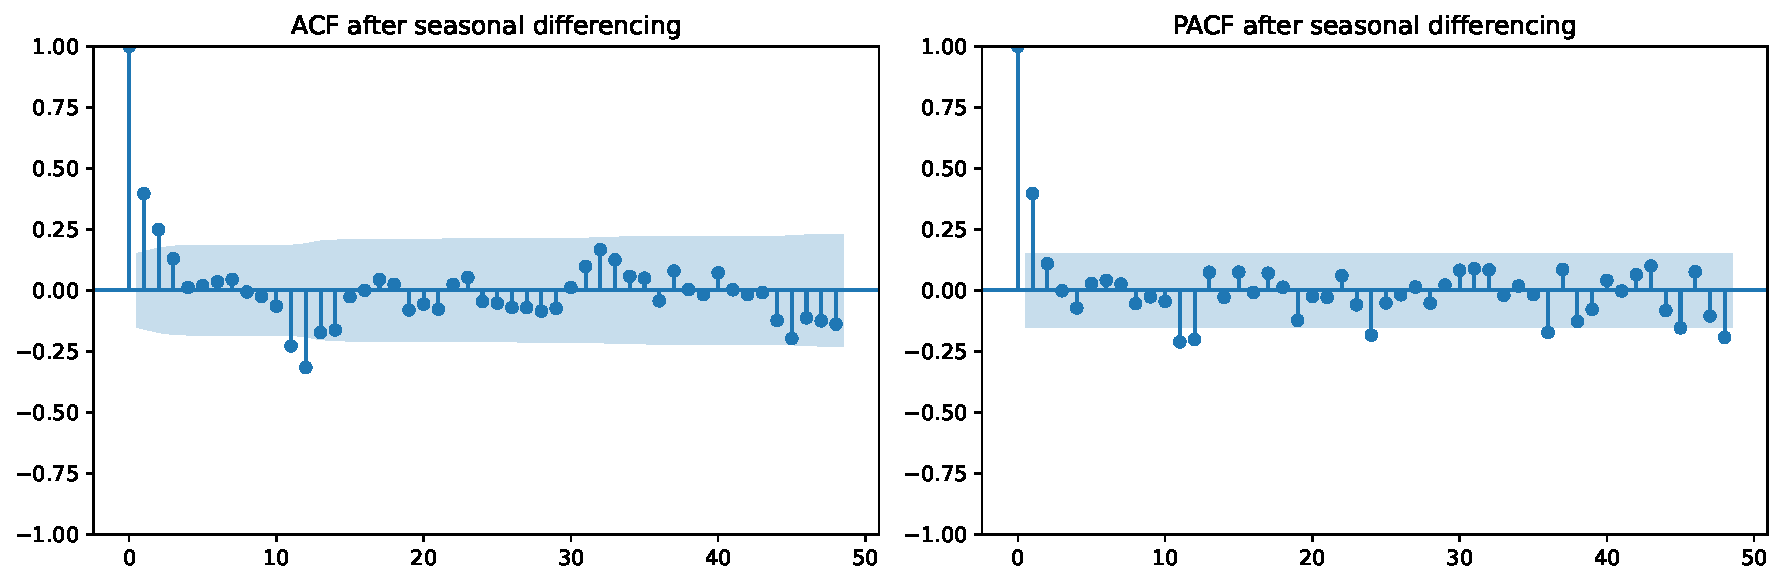
\includegraphics[keepaspectratio]{chapters/chapter-09-sarima-multiple-seasonality_files/figure-pdf/cell-3-output-2.pdf}}

When inspecting these plots, look separately at short lags and seasonal
lags. In monthly data, lags \(12,24,36,\ldots\) are especially
important.

\section{\texorpdfstring{9.19 Python example: fit SARIMA with
\texttt{statsmodels}}{9.19 Python example: fit SARIMA with statsmodels}}\label{python-example-fit-sarima-with-statsmodels}

The \texttt{SARIMAX} class in \texttt{statsmodels} fits SARIMA and
SARIMAX models. The argument \texttt{order=(p,d,q)} specifies the
nonseasonal part, and \texttt{seasonal\_order=(P,D,Q,s)} specifies the
seasonal part.

\begin{Shaded}
\begin{Highlighting}[]
\ImportTok{from}\NormalTok{ statsmodels.tsa.statespace.sarimax }\ImportTok{import}\NormalTok{ SARIMAX}

\NormalTok{train }\OperatorTok{=}\NormalTok{ series.iloc[:}\OperatorTok{{-}}\DecValTok{24}\NormalTok{]}
\NormalTok{test }\OperatorTok{=}\NormalTok{ series.iloc[}\OperatorTok{{-}}\DecValTok{24}\NormalTok{:]}

\NormalTok{model }\OperatorTok{=}\NormalTok{ SARIMAX(}
\NormalTok{    train,}
\NormalTok{    order}\OperatorTok{=}\NormalTok{(}\DecValTok{1}\NormalTok{, }\DecValTok{0}\NormalTok{, }\DecValTok{0}\NormalTok{),}
\NormalTok{    seasonal\_order}\OperatorTok{=}\NormalTok{(}\DecValTok{1}\NormalTok{, }\DecValTok{1}\NormalTok{, }\DecValTok{0}\NormalTok{, }\DecValTok{12}\NormalTok{),}
\NormalTok{    trend}\OperatorTok{=}\StringTok{"c"}\NormalTok{,}
\NormalTok{    enforce\_stationarity}\OperatorTok{=}\VariableTok{False}\NormalTok{,}
\NormalTok{    enforce\_invertibility}\OperatorTok{=}\VariableTok{False}\NormalTok{,}
\NormalTok{)}

\NormalTok{fit }\OperatorTok{=}\NormalTok{ model.fit(disp}\OperatorTok{=}\VariableTok{False}\NormalTok{)}
\BuiltInTok{print}\NormalTok{(fit.summary())}
\end{Highlighting}
\end{Shaded}

\begin{verbatim}
                                     SARIMAX Results                                      
==========================================================================================
Dep. Variable:                                  x   No. Observations:                  156
Model:             SARIMAX(1, 0, 0)x(1, 1, 0, 12)   Log Likelihood                -201.851
Date:                            Fri, 19 Jun 2026   AIC                            411.701
Time:                                    19:59:36   BIC                            423.202
Sample:                                01-01-2010   HQIC                           416.374
                                     - 12-01-2022                                         
Covariance Type:                              opg                                         
==============================================================================
                 coef    std err          z      P>|z|      [0.025      0.975]
------------------------------------------------------------------------------
intercept      0.3536      0.125      2.818      0.005       0.108       0.600
ar.L1          0.3647      0.085      4.298      0.000       0.198       0.531
ar.S.L12      -0.2783      0.089     -3.121      0.002      -0.453      -0.104
sigma2         1.2761      0.178      7.151      0.000       0.926       1.626
===================================================================================
Ljung-Box (L1) (Q):                   0.40   Jarque-Bera (JB):                 1.04
Prob(Q):                              0.53   Prob(JB):                         0.59
Heteroskedasticity (H):               1.05   Skew:                            -0.08
Prob(H) (two-sided):                  0.88   Kurtosis:                         2.59
===================================================================================

Warnings:
[1] Covariance matrix calculated using the outer product of gradients (complex-step).
\end{verbatim}

The fitted model is a candidate, not a conclusion. We still need
residual diagnostics and forecast evaluation.

\section{9.20 Python example: residual
diagnostics}\label{python-example-residual-diagnostics}

\begin{Shaded}
\begin{Highlighting}[]
\ImportTok{from}\NormalTok{ statsmodels.stats.diagnostic }\ImportTok{import}\NormalTok{ acorr\_ljungbox}
\ImportTok{import}\NormalTok{ scipy.stats }\ImportTok{as}\NormalTok{ stats}

\NormalTok{resid }\OperatorTok{=}\NormalTok{ fit.resid.dropna()}

\NormalTok{fig, axes }\OperatorTok{=}\NormalTok{ plt.subplots(}\DecValTok{2}\NormalTok{, }\DecValTok{2}\NormalTok{, figsize}\OperatorTok{=}\NormalTok{(}\DecValTok{12}\NormalTok{, }\DecValTok{8}\NormalTok{))}
\NormalTok{resid.plot(ax}\OperatorTok{=}\NormalTok{axes[}\DecValTok{0}\NormalTok{, }\DecValTok{0}\NormalTok{])}
\NormalTok{axes[}\DecValTok{0}\NormalTok{, }\DecValTok{0}\NormalTok{].set\_title(}\StringTok{"Residual time plot"}\NormalTok{)}
\NormalTok{axes[}\DecValTok{0}\NormalTok{, }\DecValTok{0}\NormalTok{].axhline(}\DecValTok{0}\NormalTok{, linewidth}\OperatorTok{=}\DecValTok{1}\NormalTok{)}

\NormalTok{plot\_acf(resid, lags}\OperatorTok{=}\DecValTok{48}\NormalTok{, ax}\OperatorTok{=}\NormalTok{axes[}\DecValTok{0}\NormalTok{, }\DecValTok{1}\NormalTok{])}
\NormalTok{axes[}\DecValTok{0}\NormalTok{, }\DecValTok{1}\NormalTok{].set\_title(}\StringTok{"Residual ACF"}\NormalTok{)}

\NormalTok{axes[}\DecValTok{1}\NormalTok{, }\DecValTok{0}\NormalTok{].hist(resid, bins}\OperatorTok{=}\DecValTok{20}\NormalTok{, density}\OperatorTok{=}\VariableTok{True}\NormalTok{, alpha}\OperatorTok{=}\FloatTok{0.7}\NormalTok{)}
\NormalTok{axes[}\DecValTok{1}\NormalTok{, }\DecValTok{0}\NormalTok{].set\_title(}\StringTok{"Residual histogram"}\NormalTok{)}

\NormalTok{stats.probplot(resid, dist}\OperatorTok{=}\StringTok{"norm"}\NormalTok{, plot}\OperatorTok{=}\NormalTok{axes[}\DecValTok{1}\NormalTok{, }\DecValTok{1}\NormalTok{])}
\NormalTok{axes[}\DecValTok{1}\NormalTok{, }\DecValTok{1}\NormalTok{].set\_title(}\StringTok{"Residual Q{-}Q plot"}\NormalTok{)}

\NormalTok{plt.tight\_layout()}
\NormalTok{plt.show()}

\NormalTok{lb }\OperatorTok{=}\NormalTok{ acorr\_ljungbox(resid, lags}\OperatorTok{=}\NormalTok{[}\DecValTok{12}\NormalTok{, }\DecValTok{24}\NormalTok{, }\DecValTok{36}\NormalTok{], return\_df}\OperatorTok{=}\VariableTok{True}\NormalTok{)}
\NormalTok{lb}
\end{Highlighting}
\end{Shaded}

\pandocbounded{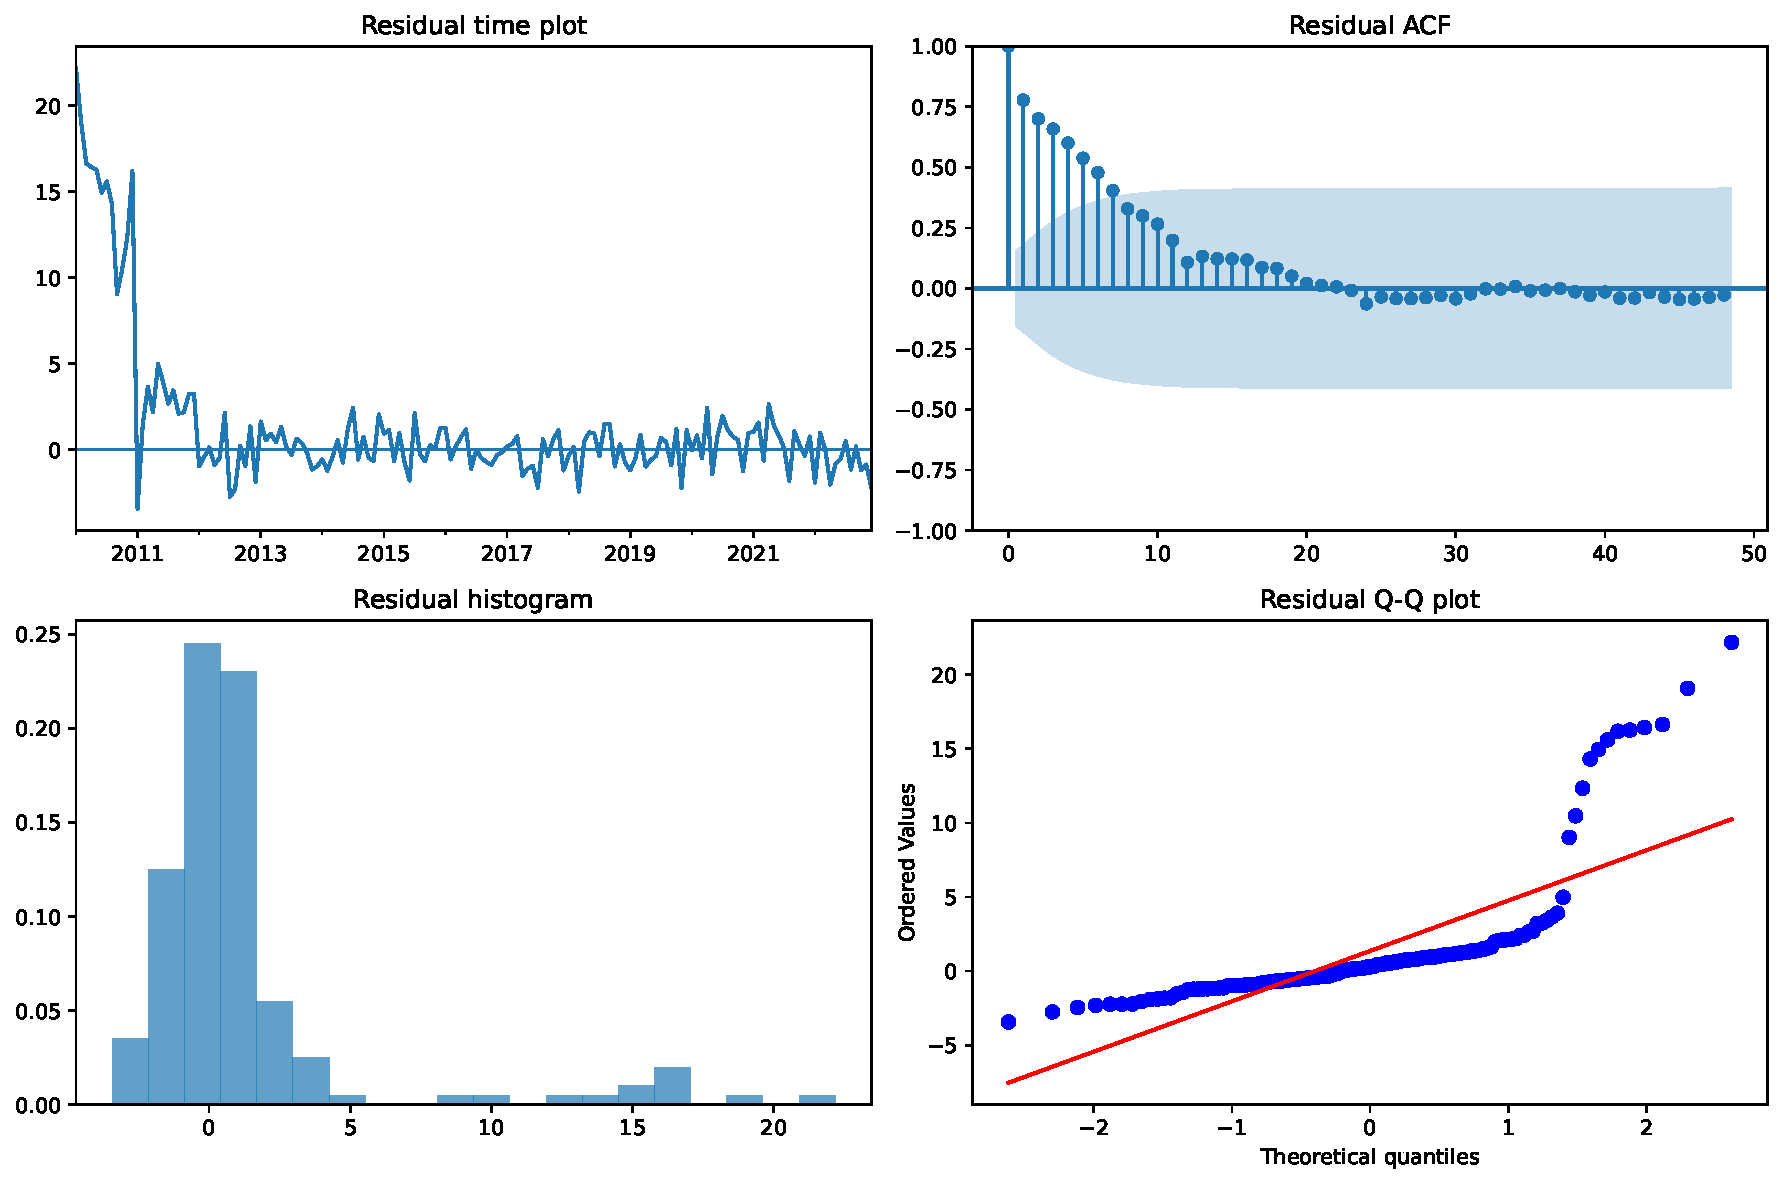
\includegraphics[keepaspectratio]{chapters/chapter-09-sarima-multiple-seasonality_files/figure-pdf/cell-5-output-1.pdf}}

{\def\LTcaptype{none} % do not increment counter
\begin{longtable}[]{@{}lll@{}}
\toprule\noalign{}
& lb\_stat & lb\_pvalue \\
\midrule\noalign{}
\endhead
\bottomrule\noalign{}
\endlastfoot
12 & 468.209521 & 1.278791e-92 \\
24 & 482.727593 & 6.389126e-87 \\
36 & 484.579207 & 6.152257e-80 \\
\end{longtable}
}

A good residual ACF should not show remaining seasonal spikes. A
significant Ljung--Box result at seasonal lags suggests that the model
has not captured all dependence.

\section{9.21 Python example: compare with seasonal naive
forecasting}\label{python-example-compare-with-seasonal-naive-forecasting}

\begin{Shaded}
\begin{Highlighting}[]
\NormalTok{forecast\_res }\OperatorTok{=}\NormalTok{ fit.get\_forecast(steps}\OperatorTok{=}\BuiltInTok{len}\NormalTok{(test))}
\NormalTok{forecast\_mean }\OperatorTok{=}\NormalTok{ forecast\_res.predicted\_mean}
\NormalTok{forecast\_ci }\OperatorTok{=}\NormalTok{ forecast\_res.conf\_int()}

\CommentTok{\# Seasonal naive baseline: repeat values from 12 months earlier.}
\NormalTok{seasonal\_naive }\OperatorTok{=}\NormalTok{ series.shift(}\DecValTok{12}\NormalTok{).loc[test.index]}

\KeywordTok{def}\NormalTok{ mae(y\_true, y\_pred):}
    \ControlFlowTok{return}\NormalTok{ np.mean(np.}\BuiltInTok{abs}\NormalTok{(np.asarray(y\_true) }\OperatorTok{{-}}\NormalTok{ np.asarray(y\_pred)))}

\KeywordTok{def}\NormalTok{ rmse(y\_true, y\_pred):}
    \ControlFlowTok{return}\NormalTok{ np.sqrt(np.mean((np.asarray(y\_true) }\OperatorTok{{-}}\NormalTok{ np.asarray(y\_pred))}\OperatorTok{**}\DecValTok{2}\NormalTok{))}

\NormalTok{comparison }\OperatorTok{=}\NormalTok{ pd.DataFrame(\{}
    \StringTok{"MAE"}\NormalTok{: [mae(test, forecast\_mean), mae(test, seasonal\_naive)],}
    \StringTok{"RMSE"}\NormalTok{: [rmse(test, forecast\_mean), rmse(test, seasonal\_naive)],}
\NormalTok{\}, index}\OperatorTok{=}\NormalTok{[}\StringTok{"SARIMA candidate"}\NormalTok{, }\StringTok{"Seasonal naive"}\NormalTok{])}

\BuiltInTok{print}\NormalTok{(comparison)}

\NormalTok{fig, ax }\OperatorTok{=}\NormalTok{ plt.subplots(figsize}\OperatorTok{=}\NormalTok{(}\DecValTok{10}\NormalTok{, }\DecValTok{4}\NormalTok{))}
\NormalTok{train.iloc[}\OperatorTok{{-}}\DecValTok{48}\NormalTok{:].plot(ax}\OperatorTok{=}\NormalTok{ax, label}\OperatorTok{=}\StringTok{"train"}\NormalTok{)}
\NormalTok{test.plot(ax}\OperatorTok{=}\NormalTok{ax, label}\OperatorTok{=}\StringTok{"test"}\NormalTok{)}
\NormalTok{forecast\_mean.plot(ax}\OperatorTok{=}\NormalTok{ax, label}\OperatorTok{=}\StringTok{"SARIMA forecast"}\NormalTok{)}
\NormalTok{seasonal\_naive.plot(ax}\OperatorTok{=}\NormalTok{ax, label}\OperatorTok{=}\StringTok{"seasonal naive"}\NormalTok{, linestyle}\OperatorTok{=}\StringTok{"{-}{-}"}\NormalTok{)}
\NormalTok{ax.fill\_between(}
\NormalTok{    test.index,}
\NormalTok{    forecast\_ci.iloc[:, }\DecValTok{0}\NormalTok{],}
\NormalTok{    forecast\_ci.iloc[:, }\DecValTok{1}\NormalTok{],}
\NormalTok{    alpha}\OperatorTok{=}\FloatTok{0.2}\NormalTok{,}
\NormalTok{    label}\OperatorTok{=}\StringTok{"SARIMA 95}\SpecialCharTok{\% i}\StringTok{nterval"}\NormalTok{,}
\NormalTok{)}
\NormalTok{ax.set\_title(}\StringTok{"SARIMA forecast versus seasonal naive baseline"}\NormalTok{)}
\NormalTok{ax.legend()}
\NormalTok{plt.show()}
\end{Highlighting}
\end{Shaded}

\begin{verbatim}
                       MAE      RMSE
SARIMA candidate  1.034198  1.267995
Seasonal naive    1.192679  1.429458
\end{verbatim}

\pandocbounded{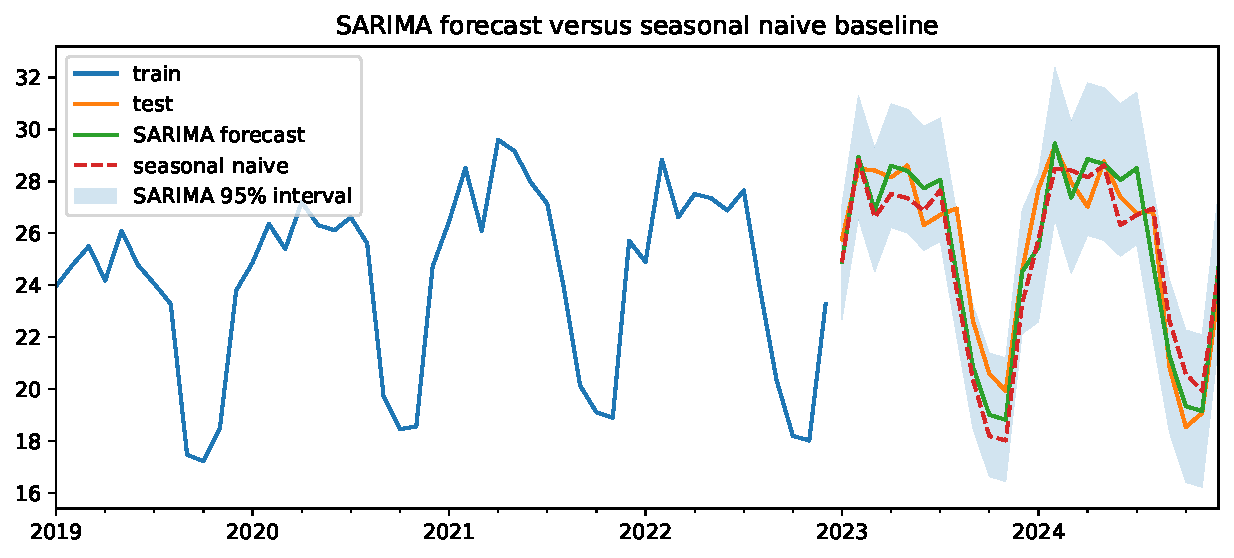
\includegraphics[keepaspectratio]{chapters/chapter-09-sarima-multiple-seasonality_files/figure-pdf/cell-6-output-2.pdf}}

A SARIMA model should be judged against a baseline. If it cannot improve
on seasonal naive forecasting, then the extra complexity may not be
useful.

\section{9.22 Python example: Fourier features for multiple
seasonality}\label{python-example-fourier-features-for-multiple-seasonality}

SARIMA is usually designed around one seasonal period. For multiple
seasonalities, Fourier features provide a flexible alternative.

The function below builds Fourier features for a given period \(m\) and
order \(K\).

\begin{Shaded}
\begin{Highlighting}[]
\KeywordTok{def}\NormalTok{ fourier\_features(index, period, K, prefix):}
\NormalTok{    t }\OperatorTok{=}\NormalTok{ np.arange(}\BuiltInTok{len}\NormalTok{(index))}
\NormalTok{    data }\OperatorTok{=}\NormalTok{ \{\}}
    \ControlFlowTok{for}\NormalTok{ k }\KeywordTok{in} \BuiltInTok{range}\NormalTok{(}\DecValTok{1}\NormalTok{, K }\OperatorTok{+} \DecValTok{1}\NormalTok{):}
\NormalTok{        data[}\SpecialStringTok{f"}\SpecialCharTok{\{}\NormalTok{prefix}\SpecialCharTok{\}}\SpecialStringTok{\_sin\_}\SpecialCharTok{\{}\NormalTok{k}\SpecialCharTok{\}}\SpecialStringTok{"}\NormalTok{] }\OperatorTok{=}\NormalTok{ np.sin(}\DecValTok{2}\OperatorTok{*}\NormalTok{np.pi}\OperatorTok{*}\NormalTok{k}\OperatorTok{*}\NormalTok{t}\OperatorTok{/}\NormalTok{period)}
\NormalTok{        data[}\SpecialStringTok{f"}\SpecialCharTok{\{}\NormalTok{prefix}\SpecialCharTok{\}}\SpecialStringTok{\_cos\_}\SpecialCharTok{\{}\NormalTok{k}\SpecialCharTok{\}}\SpecialStringTok{"}\NormalTok{] }\OperatorTok{=}\NormalTok{ np.cos(}\DecValTok{2}\OperatorTok{*}\NormalTok{np.pi}\OperatorTok{*}\NormalTok{k}\OperatorTok{*}\NormalTok{t}\OperatorTok{/}\NormalTok{period)}
    \ControlFlowTok{return}\NormalTok{ pd.DataFrame(data, index}\OperatorTok{=}\NormalTok{index)}

\CommentTok{\# Example: yearly seasonality for monthly data has period 12.}
\NormalTok{X\_fourier }\OperatorTok{=}\NormalTok{ fourier\_features(series.index, period}\OperatorTok{=}\DecValTok{12}\NormalTok{, K}\OperatorTok{=}\DecValTok{2}\NormalTok{, prefix}\OperatorTok{=}\StringTok{"year"}\NormalTok{)}
\NormalTok{X\_fourier.head()}
\end{Highlighting}
\end{Shaded}

{\def\LTcaptype{none} % do not increment counter
\begin{longtable}[]{@{}lllll@{}}
\toprule\noalign{}
& year\_sin\_1 & year\_cos\_1 & year\_sin\_2 & year\_cos\_2 \\
\midrule\noalign{}
\endhead
\bottomrule\noalign{}
\endlastfoot
2010-01-01 & 0.000000 & 1.000000e+00 & 0.000000e+00 & 1.0 \\
2010-02-01 & 0.500000 & 8.660254e-01 & 8.660254e-01 & 0.5 \\
2010-03-01 & 0.866025 & 5.000000e-01 & 8.660254e-01 & -0.5 \\
2010-04-01 & 1.000000 & 6.123234e-17 & 1.224647e-16 & -1.0 \\
2010-05-01 & 0.866025 & -5.000000e-01 & -8.660254e-01 & -0.5 \\
\end{longtable}
}

These features can be used in regression, SARIMAX, gradient boosting,
neural networks, or transformer models. In longer daily or hourly
series, Fourier features are often more stable than trying to fit very
high-order seasonal ARIMA terms.

\section{9.23 AI-assisted study: seasonal model
critic}\label{ai-assisted-study-seasonal-model-critic}

Use AI as a critic, not as an oracle. A useful prompt is:

\begin{quote}
I have monthly data with strong yearly seasonality. I fit
SARIMA\((1,1,1)(0,1,1)_{12}\). The residual ACF still has a significant
spike at lag 12 and the Ljung--Box test at lag 24 has \(p<0.01\). Give
possible explanations and suggest diagnostic checks. Do not choose a
final model until the residual plots and backtesting results are
inspected.
\end{quote}

Then verify the response manually:

\begin{enumerate}
\def\labelenumi{\arabic{enumi}.}
\tightlist
\item
  Did the AI distinguish seasonal and nonseasonal differencing?
\item
  Did it mention residual seasonality?
\item
  Did it avoid claiming that AIC alone proves a model is best?
\item
  Did it recommend comparing with seasonal naive forecasting?
\item
  Did it ask about transformations, outliers, and structural breaks?
\end{enumerate}

A second useful prompt is:

\begin{quote}
Explain the difference between deterministic seasonal dummy variables,
Fourier seasonal regressors, seasonal differencing, and a seasonal AR
term. Give one example where each is appropriate.
\end{quote}

This helps students connect modeling choices to assumptions.

\section{9.24 Common mistakes}\label{common-mistakes-8}

\begin{enumerate}
\def\labelenumi{\arabic{enumi}.}
\tightlist
\item
  \textbf{Forgetting the seasonal naive baseline.} A complicated SARIMA
  model may not beat last season's value.
\item
  \textbf{Using the wrong seasonal period.} Domain knowledge matters.
  Daily data may have weekly, annual, and holiday patterns.
\item
  \textbf{Over-differencing.} Applying both \(d=1\) and \(D=1\) without
  checking the transformed series can create artificial dependence.
\item
  \textbf{Reading only short lags.} Seasonal models require inspecting
  \(s,2s,3s,\ldots\).
\item
  \textbf{Trusting AIC alone.} A model with lower AIC can forecast worse
  out of sample.
\item
  \textbf{Ignoring calendar effects.} Holidays and interventions are not
  the same as regular seasonality.
\item
  \textbf{Confusing deterministic and stochastic seasonality.} Seasonal
  dummies, Fourier features, and seasonal differencing answer different
  modeling questions.
\item
  \textbf{Using SARIMA for every seasonal problem.} Multiple
  seasonality, irregular data, and many related series often need other
  tools.
\end{enumerate}

\section{9.25 Mini project: monthly demand
forecasting}\label{mini-project-monthly-demand-forecasting}

Choose a monthly seasonal data set such as airline passengers, product
demand, tourism counts, or public transit ridership.

Your report should include:

\begin{enumerate}
\def\labelenumi{\arabic{enumi}.}
\tightlist
\item
  a time plot and seasonal plot;
\item
  variance-stabilizing transformation if needed;
\item
  justification for \(s\), \(D\), and \(d\);
\item
  ACF/PACF of the transformed series;
\item
  at least three candidate SARIMA models;
\item
  residual diagnostics for the selected model;
\item
  comparison with seasonal naive forecasting;
\item
  forecast plot with intervals;
\item
  a short AI-assisted critique and your verification of that critique.
\end{enumerate}

\section{9.26 Exercises}\label{exercises-8}

\subsection{Conceptual exercises}\label{conceptual-exercises-7}

\begin{enumerate}
\def\labelenumi{\arabic{enumi}.}
\tightlist
\item
  Explain why SARIMA\((0,0,0)(0,1,0)_{12}\) is a seasonal random walk.
\item
  For monthly data, what lags should you inspect first when diagnosing
  seasonal dependence?
\item
  Explain the difference between \(d=1\) and \(D=1\).
\item
  Why can seasonal differencing remove a deterministic seasonal mean but
  still change the stationary error process?
\item
  Why is seasonal naive forecasting a strong baseline?
\end{enumerate}

\subsection{Mathematical exercises}\label{mathematical-exercises-6}

\begin{enumerate}
\def\labelenumi{\arabic{enumi}.}
\tightlist
\item
  Expand \((1-B)(1-B^{12})X_t\).
\item
  Expand \((1-\phi B)(1-\Phi B^{s})X_t\) and interpret each term.
\item
  Expand \((1+\theta B)(1+\Theta B^{s})W_t\).
\item
  Show that if \(X_t=X_{t-s}+W_t\), then \(\nabla_sX_t\) is white noise.
\item
  For \(X_t=\Phi X_{t-s}+W_t\) with \(|\Phi|<1\), derive the causal
  representation \[
  X_t=\sum_{j=0}^{\infty}\Phi^j W_{t-js}.
  \]
\item
  For the same model, compute \(\gamma(0)\) and \(\gamma(s)\).
\item
  Explain why the ACF of a pure seasonal MA\((1)_s\) cuts off after lag
  \(s\) at the seasonal scale.
\item
  For SARIMA\((1,0,0)(1,0,0)_{12}\), list all AR lags that appear after
  expansion.
\end{enumerate}

\subsection{Computational exercises}\label{computational-exercises-4}

\begin{enumerate}
\def\labelenumi{\arabic{enumi}.}
\tightlist
\item
  Simulate a pure seasonal AR\((1)_{12}\) model for \(\Phi=0.2,0.6,0.9\)
  and compare ACFs.
\item
  Simulate a seasonal random walk and show that seasonal differencing
  produces a stationary-looking series.
\item
  Fit SARIMA\((0,1,1)(0,1,1)_{12}\) to a monthly data set and check
  residuals.
\item
  Compare SARIMA with seasonal naive forecasting using rolling-origin
  validation.
\item
  Add Fourier features to a regression model and compare it with SARIMA.
\item
  Create artificial holiday effects and show that SARIMA alone may leave
  systematic residual errors.
\end{enumerate}

\section{9.27 Chapter checklist}\label{chapter-checklist-6}

Before moving on, make sure you can:

\begin{itemize}
\tightlist
\item
  write \(B^sX_t=X_{t-s}\) and \(\nabla_sX_t=(1-B^s)X_t\);
\item
  define SARIMA\((p,d,q)(P,D,Q)_s\);
\item
  expand simple multiplicative seasonal polynomials;
\item
  distinguish seasonal AR, seasonal MA, and seasonal differencing;
\item
  read ACF/PACF at seasonal lags;
\item
  fit a SARIMA model in Python;
\item
  diagnose residual seasonality;
\item
  compare against a seasonal naive baseline;
\item
  explain when Fourier features or modern ML models may be preferable to
  a single-period SARIMA model.
\end{itemize}

\chapter{State-Space Models and Kalman
Filtering}\label{state-space-models-and-kalman-filtering}

\textbf{Part III. Nonstationary and Seasonal Models}\\
\textbf{Chapter goal:} learn how to represent time series through hidden
dynamic states and update uncertainty sequentially. We develop linear
Gaussian state-space models, Kalman prediction and update equations,
local-level and local-linear trend models, missing-data handling,
forecasting, smoothing, likelihood evaluation, and connections to modern
sequence learning and AI-assisted modeling.

\section{Learning objectives}\label{learning-objectives-9}

After studying this chapter, you should be able to:

\begin{enumerate}
\def\labelenumi{\arabic{enumi}.}
\tightlist
\item
  explain why a hidden-state representation is useful for time series
  forecasting, filtering, and smoothing;
\item
  write a linear Gaussian state-space model using observation and state
  equations;
\item
  derive the Kalman filter from conditional Gaussian projection
  formulas;
\item
  implement the prediction, innovation, Kalman gain, and update steps;
\item
  interpret the local-level and local-linear trend models;
\item
  compute forecast distributions and prediction intervals from the
  filtering recursions;
\item
  handle missing observations naturally inside a state-space model;
\item
  distinguish filtering, forecasting, and smoothing;
\item
  connect ARIMA-type models, dynamic regression, HMMs, RNNs, and
  attention models through the hidden-state viewpoint;
\item
  use AI tools to debug recursive algorithms while verifying dimensions,
  assumptions, and numerical stability manually.
\end{enumerate}

\section{10.1 From observed series to hidden dynamic
states}\label{from-observed-series-to-hidden-dynamic-states}

Classical ARIMA and SARIMA models describe \(X_t\) directly in terms of
past observations and past shocks. State-space models introduce an
additional layer: an unobserved state vector \(\boldsymbol{\alpha}_t\)
that evolves over time and generates the observed series.

The basic idea is:

\[
\text{hidden state at time } t \longrightarrow \text{observation at time } t.
\]

For example, suppose the observed series is noisy sales demand. The
hidden state might contain:

\[
\boldsymbol{\alpha}_t=
\begin{bmatrix}
\text{current level}\\
\text{current trend}\\
\text{seasonal component}
\end{bmatrix}.
\]

The observed value \(y_t\) is noisy, but the hidden state evolves
smoothly. The goal is to update our belief about the state as
observations arrive.

\begin{tcolorbox}[enhanced jigsaw, arc=.35mm, bottomrule=.15mm, bottomtitle=1mm, breakable, colback=white, colbacktitle=quarto-callout-note-color!10!white, colframe=quarto-callout-note-color-frame, coltitle=black, left=2mm, leftrule=.75mm, opacityback=0, opacitybacktitle=0.6, rightrule=.15mm, title=\textcolor{quarto-callout-note-color}{\faInfo}\hspace{0.5em}{Three related tasks}, titlerule=0mm, toprule=.15mm, toptitle=1mm]

At time \(t\), we distinguish three tasks:

\begin{itemize}
\tightlist
\item
  \textbf{Filtering:} estimate \(\boldsymbol{\alpha}_t\) using data
  through time \(t\).
\item
  \textbf{Forecasting:} estimate future states or observations using
  data through time \(t\).
\item
  \textbf{Smoothing:} estimate past states using data from the full
  sample.
\end{itemize}

\end{tcolorbox}

This chapter focuses on linear Gaussian state-space models, where all
conditional distributions are Gaussian and the Kalman filter gives exact
recursive formulas.

\section{10.2 The linear Gaussian state-space
model}\label{the-linear-gaussian-state-space-model}

A standard time-invariant linear Gaussian state-space model is

\[
y_t=\mathbf{F}^\top \boldsymbol{\alpha}_t+v_t,
\qquad v_t\sim N(0,V),
\]

and

\[
\boldsymbol{\alpha}_t=\mathbf{G}\boldsymbol{\alpha}_{t-1}+\mathbf{w}_t,
\qquad \mathbf{w}_t\sim N(\mathbf{0},\mathbf{W}).
\]

Here:

\begin{itemize}
\tightlist
\item
  \(y_t\in \mathbb{R}\) is the observed value;
\item
  \(\boldsymbol{\alpha}_t\in\mathbb{R}^d\) is the hidden state vector;
\item
  \(\mathbf{F}\in\mathbb{R}^d\) maps the state to the observation;
\item
  \(\mathbf{G}\in\mathbb{R}^{d\times d}\) evolves the hidden state;
\item
  \(V>0\) is the observation-noise variance;
\item
  \(\mathbf{W}\) is the state-noise covariance matrix.
\end{itemize}

More generally, these quantities may vary with time:

\[
y_t=\mathbf{F}_t^\top \boldsymbol{\alpha}_t+v_t,
\qquad v_t\sim N(0,V_t),
\]

\[
\boldsymbol{\alpha}_t=\mathbf{G}_t\boldsymbol{\alpha}_{t-1}+\mathbf{w}_t,
\qquad \mathbf{w}_t\sim N(\mathbf{0},\mathbf{W}_t).
\]

We also need an initial belief:

\[
\boldsymbol{\alpha}_0\mid \mathcal{D}_0\sim N(\mathbf{m}_0,\mathbf{C}_0),
\]

where \(\mathcal{D}_t=\{y_1,\ldots,y_t\}\) denotes the observed data
through time \(t\).

\begin{tcolorbox}[enhanced jigsaw, arc=.35mm, bottomrule=.15mm, bottomtitle=1mm, breakable, colback=white, colbacktitle=quarto-callout-tip-color!10!white, colframe=quarto-callout-tip-color-frame, coltitle=black, left=2mm, leftrule=.75mm, opacityback=0, opacitybacktitle=0.6, rightrule=.15mm, title=\textcolor{quarto-callout-tip-color}{\faLightbulb}\hspace{0.5em}{Interpretation}, titlerule=0mm, toprule=.15mm, toptitle=1mm]

The Kalman filter is a recursive Bayesian update for this model. Before
observing \(y_t\), we have a predicted distribution for
\(\boldsymbol{\alpha}_t\). After observing \(y_t\), we update the
distribution using the prediction error.

\end{tcolorbox}

\section{10.3 Conditional Gaussian
updating}\label{conditional-gaussian-updating}

The Kalman filter is easiest to understand through a basic fact about
jointly Gaussian random variables.

Suppose

\[
\begin{bmatrix}
\mathbf{x}\\
y
\end{bmatrix}
\sim N\left(
\begin{bmatrix}
\mathbf{a}\\
f
\end{bmatrix},
\begin{bmatrix}
\mathbf{R} & \mathbf{r}\\
\mathbf{r}^\top & Q
\end{bmatrix}
\right).
\]

Then the conditional distribution of \(\mathbf{x}\) given \(y\) is
Gaussian:

\[
\mathbf{x}\mid y\sim N\left(\mathbf{a}+\mathbf{r}Q^{-1}(y-f),\;\mathbf{R}-\mathbf{r}Q^{-1}\mathbf{r}^\top\right).
\]

In the state-space setting:

\begin{itemize}
\tightlist
\item
  \(\mathbf{x}\) is the hidden state \(\boldsymbol{\alpha}_t\);
\item
  \(y\) is the observation \(y_t\);
\item
  \(f\) is the one-step forecast of \(y_t\);
\item
  \(y_t-f_t\) is the innovation, or prediction error;
\item
  \(\mathbf{r}Q^{-1}\) becomes the Kalman gain.
\end{itemize}

So the update has a simple geometric interpretation:

\[
\text{updated state}=   ext{predicted state}+\text{gain}\times\text{prediction error}.
\]

\section{10.4 Kalman filter notation}\label{kalman-filter-notation}

We use the following notation.

The \textbf{filtered distribution} at time \(t-1\) is

\[
\boldsymbol{\alpha}_{t-1}\mid \mathcal{D}_{t-1}
\sim N(\mathbf{m}_{t-1},\mathbf{C}_{t-1}).
\]

The \textbf{one-step predicted state distribution} is

\[
\boldsymbol{\alpha}_{t}\mid \mathcal{D}_{t-1}
\sim N(\mathbf{a}_{t},\mathbf{R}_{t}).
\]

The \textbf{one-step forecast distribution} for the observation is

\[
y_t\mid \mathcal{D}_{t-1}
\sim N(f_t,Q_t).
\]

The \textbf{filtered distribution} after observing \(y_t\) is

\[
\boldsymbol{\alpha}_{t}\mid \mathcal{D}_{t}
\sim N(\mathbf{m}_{t},\mathbf{C}_{t}).
\]

The Kalman filter recursively maps

\[
(\mathbf{m}_{t-1},\mathbf{C}_{t-1})
\longrightarrow
(\mathbf{a}_{t},\mathbf{R}_{t})
\longrightarrow
(f_t,Q_t)
\longrightarrow
(\mathbf{m}_{t},\mathbf{C}_{t}).
\]

\section{10.5 Prediction step}\label{prediction-step}

Start with

\[
\boldsymbol{\alpha}_{t-1}\mid \mathcal{D}_{t-1}
\sim N(\mathbf{m}_{t-1},\mathbf{C}_{t-1}).
\]

Using the state equation

\[
\boldsymbol{\alpha}_t=\mathbf{G}\boldsymbol{\alpha}_{t-1}+\mathbf{w}_t,
\]

we obtain

\[
\mathbf{a}_t=\mathbf{G}\mathbf{m}_{t-1},
\]

and

\[
\mathbf{R}_t=\mathbf{G}\mathbf{C}_{t-1}\mathbf{G}^\top+\mathbf{W}.
\]

So

\[
\boldsymbol{\alpha}_{t}\mid \mathcal{D}_{t-1}
\sim N(\mathbf{a}_{t},\mathbf{R}_{t}).
\]

The extra term \(\mathbf{W}\) increases uncertainty because the state
evolves with random noise.

\section{10.6 Forecast step}\label{forecast-step}

Using the observation equation

\[
y_t=\mathbf{F}^\top\boldsymbol{\alpha}_t+v_t,
\]

and the predicted state distribution, we get

\[
f_t=\mathbf{F}^\top\mathbf{a}_t,
\]

and

\[
Q_t=\mathbf{F}^\top\mathbf{R}_t\mathbf{F}+V.
\]

The innovation is

\[
e_t=y_t-f_t.
\]

Thus

\[
y_t\mid\mathcal{D}_{t-1}\sim N(f_t,Q_t).
\]

A \(95\%\) one-step prediction interval is approximately

\[
f_t\pm 1.96\sqrt{Q_t}.
\]

\section{10.7 Update step}\label{update-step}

The Kalman gain is

\[
\mathbf{A}_t=\mathbf{R}_t\mathbf{F}Q_t^{-1}.
\]

Then the updated state mean is

\[
\mathbf{m}_t=\mathbf{a}_t+\mathbf{A}_t e_t.
\]

The updated state covariance is

\[
\mathbf{C}_t=\mathbf{R}_t-\mathbf{A}_tQ_t\mathbf{A}_t^\top.
\]

Equivalently,

\[
\mathbf{C}_t=\mathbf{R}_t-\mathbf{R}_t\mathbf{F}Q_t^{-1}\mathbf{F}^\top\mathbf{R}_t.
\]

\begin{tcolorbox}[enhanced jigsaw, arc=.35mm, bottomrule=.15mm, bottomtitle=1mm, breakable, colback=white, colbacktitle=quarto-callout-note-color!10!white, colframe=quarto-callout-note-color-frame, coltitle=black, left=2mm, leftrule=.75mm, opacityback=0, opacitybacktitle=0.6, rightrule=.15mm, title=\textcolor{quarto-callout-note-color}{\faInfo}\hspace{0.5em}{Why the gain matters}, titlerule=0mm, toprule=.15mm, toptitle=1mm]

If observation noise \(V\) is large, then \(Q_t\) is large and the gain
is small. The filter trusts the model more than the new observation.

If state uncertainty \(\mathbf{R}_t\) is large, then the gain is larger.
The filter learns more from the new observation.

\end{tcolorbox}

\section{10.8 Algorithm summary}\label{algorithm-summary}

For \(t=1,2,\ldots,n\):

\begin{enumerate}
\def\labelenumi{\arabic{enumi}.}
\tightlist
\item
  \textbf{Predict state}
\end{enumerate}

\[
\mathbf{a}_t=\mathbf{G}\mathbf{m}_{t-1},
\qquad
\mathbf{R}_t=\mathbf{G}\mathbf{C}_{t-1}\mathbf{G}^\top+\mathbf{W}.
\]

\begin{enumerate}
\def\labelenumi{\arabic{enumi}.}
\setcounter{enumi}{1}
\tightlist
\item
  \textbf{Forecast observation}
\end{enumerate}

\[
f_t=\mathbf{F}^\top\mathbf{a}_t,
\qquad
Q_t=\mathbf{F}^\top\mathbf{R}_t\mathbf{F}+V.
\]

\begin{enumerate}
\def\labelenumi{\arabic{enumi}.}
\setcounter{enumi}{2}
\tightlist
\item
  \textbf{Compute innovation}
\end{enumerate}

\[
e_t=y_t-f_t.
\]

\begin{enumerate}
\def\labelenumi{\arabic{enumi}.}
\setcounter{enumi}{3}
\tightlist
\item
  \textbf{Compute gain}
\end{enumerate}

\[
\mathbf{A}_t=\mathbf{R}_t\mathbf{F}Q_t^{-1}.
\]

\begin{enumerate}
\def\labelenumi{\arabic{enumi}.}
\setcounter{enumi}{4}
\tightlist
\item
  \textbf{Update state}
\end{enumerate}

\[
\mathbf{m}_t=\mathbf{a}_t+\mathbf{A}_t e_t,
\qquad
\mathbf{C}_t=\mathbf{R}_t-\mathbf{A}_tQ_t\mathbf{A}_t^\top.
\]

\begin{tcolorbox}[enhanced jigsaw, arc=.35mm, bottomrule=.15mm, bottomtitle=1mm, breakable, colback=white, colbacktitle=quarto-callout-warning-color!10!white, colframe=quarto-callout-warning-color-frame, coltitle=black, left=2mm, leftrule=.75mm, opacityback=0, opacitybacktitle=0.6, rightrule=.15mm, title=\textcolor{quarto-callout-warning-color}{\faExclamationTriangle}\hspace{0.5em}{Dimension check}, titlerule=0mm, toprule=.15mm, toptitle=1mm]

If \(\boldsymbol{\alpha}_t\in\mathbb{R}^d\), then

\[
\mathbf{F}\in\mathbb{R}^d,
\quad
\mathbf{G}\in\mathbb{R}^{d\times d},
\quad
\mathbf{W}\in\mathbb{R}^{d\times d},
\quad
\mathbf{A}_t\in\mathbb{R}^d.
\]

Dimension errors are the most common implementation mistakes.

\end{tcolorbox}

\section{10.9 Local-level model}\label{local-level-model}

The simplest useful state-space model is the local-level model:

\[
y_t=\mu_t+v_t,
\qquad v_t\sim N(0,V),
\]

\[
\mu_t=\mu_{t-1}+w_t,
\qquad w_t\sim N(0,W).
\]

Here the hidden state is one-dimensional:

\[
\boldsymbol{\alpha}_t=\mu_t.
\]

Thus

\[
\mathbf{F}=1,
\qquad
\mathbf{G}=1.
\]

The Kalman equations reduce to scalar recursions:

\[
a_t=m_{t-1},
\qquad
R_t=C_{t-1}+W,
\]

\[
f_t=a_t,
\qquad
Q_t=R_t+V,
\]

\[
A_t=\frac{R_t}{Q_t},
\]

\[
m_t=a_t+A_t(y_t-a_t),
\]

\[
C_t=R_t-A_t^2Q_t=R_t\left(1-\frac{R_t}{Q_t}\right).
\]

Since \(Q_t=R_t+V\), the scalar gain is

\[
A_t=\frac{R_t}{R_t+V}.
\]

If \(V\) is large, then \(A_t\) is small. If \(R_t\) is large, then
\(A_t\) is large.

\begin{tcolorbox}[enhanced jigsaw, arc=.35mm, bottomrule=.15mm, bottomtitle=1mm, breakable, colback=white, colbacktitle=quarto-callout-tip-color!10!white, colframe=quarto-callout-tip-color-frame, coltitle=black, left=2mm, leftrule=.75mm, opacityback=0, opacitybacktitle=0.6, rightrule=.15mm, title=\textcolor{quarto-callout-tip-color}{\faLightbulb}\hspace{0.5em}{Local-level intuition}, titlerule=0mm, toprule=.15mm, toptitle=1mm]

The local-level model is a smoothed random walk observed with noise. It
is useful when the true level evolves slowly but observations are noisy.

\end{tcolorbox}

\section{10.10 Local-linear trend model}\label{local-linear-trend-model}

The local-level model allows the level to change but does not explicitly
model slope. A local-linear trend model has two hidden components:

\[
\boldsymbol{\alpha}_t=
\begin{bmatrix}
\mu_t\\
\beta_t
\end{bmatrix},
\]

where \(\mu_t\) is the level and \(\beta_t\) is the slope.

A common specification is

\[
y_t=\mu_t+v_t,
\]

\[
\mu_t=\mu_{t-1}+\beta_{t-1}+w_{1,t},
\]

\[
\beta_t=\beta_{t-1}+w_{2,t}.
\]

In matrix form:

\[
y_t=
\begin{bmatrix}1 & 0\end{bmatrix}
\begin{bmatrix}
\mu_t\\
\beta_t
\end{bmatrix}+v_t,
\]

and

\[
\begin{bmatrix}
\mu_t\\
\beta_t
\end{bmatrix}
=
\begin{bmatrix}
1 & 1\\
0 & 1
\end{bmatrix}
\begin{bmatrix}
\mu_{t-1}\\
\beta_{t-1}
\end{bmatrix}
+
\begin{bmatrix}
w_{1,t}\\
w_{2,t}
\end{bmatrix}.
\]

So

\[
\mathbf{F}=\begin{bmatrix}1\\0\end{bmatrix},
\qquad
\mathbf{G}=\begin{bmatrix}1&1\\0&1\end{bmatrix}.
\]

This is a dynamic version of a line. The intercept and slope evolve over
time.

\section{10.11 AR(1) as a state-space
model}\label{ar1-as-a-state-space-model}

An AR(1) model is

\[
y_t=\phi y_{t-1}+w_t.
\]

It can be written as a state-space model with the hidden state
\(\alpha_t=y_t\):

\[
\alpha_t=\phi\alpha_{t-1}+w_t,
\]

\[
y_t=\alpha_t+v_t.
\]

If \(v_t=0\), then the observation is exact. If \(v_t\) is nonzero, this
becomes a noisy AR(1) state process.

This perspective shows that AR models are special cases of state-space
models. State-space models are more flexible because they can include
trends, seasonality, regression effects, missing observations, and
measurement noise in one unified framework.

\section{10.12 Forecasting with a state-space
model}\label{forecasting-with-a-state-space-model}

Given the filtered state distribution at time \(t\),

\[
\boldsymbol{\alpha}_t\mid\mathcal{D}_t\sim N(\mathbf{m}_t,\mathbf{C}_t),
\]

we can forecast \(h\) steps ahead by repeatedly applying the state
equation.

For time-invariant \(\mathbf{G}\),

\[
\mathbf{a}_{t+h|t}=\mathbf{G}^h\mathbf{m}_t.
\]

The \(h\)-step state covariance is

\[
\mathbf{R}_{t+h|t}
=\mathbf{G}^h\mathbf{C}_t(\mathbf{G}^h)^\top
+\sum_{j=0}^{h-1}\mathbf{G}^j\mathbf{W}(\mathbf{G}^j)^\top.
\]

Then the \(h\)-step forecast distribution for the observation is

\[
y_{t+h}\mid\mathcal{D}_t
\sim N(f_{t+h|t},Q_{t+h|t}),
\]

where

\[
f_{t+h|t}=\mathbf{F}^\top\mathbf{a}_{t+h|t},
\]

and

\[
Q_{t+h|t}=\mathbf{F}^\top\mathbf{R}_{t+h|t}\mathbf{F}+V.
\]

\section{10.13 Missing observations}\label{missing-observations}

A major advantage of the Kalman filter is that it handles missing
observations naturally.

Suppose \(y_t\) is missing. We still perform the state prediction:

\[
\mathbf{a}_t=\mathbf{G}\mathbf{m}_{t-1},
\qquad
\mathbf{R}_t=\mathbf{G}\mathbf{C}_{t-1}\mathbf{G}^\top+\mathbf{W}.
\]

But we skip the observation update:

\[
\mathbf{m}_t=\mathbf{a}_t,
\qquad
\mathbf{C}_t=\mathbf{R}_t.
\]

The uncertainty grows because no new information is available at that
time.

\begin{tcolorbox}[enhanced jigsaw, arc=.35mm, bottomrule=.15mm, bottomtitle=1mm, breakable, colback=white, colbacktitle=quarto-callout-note-color!10!white, colframe=quarto-callout-note-color-frame, coltitle=black, left=2mm, leftrule=.75mm, opacityback=0, opacitybacktitle=0.6, rightrule=.15mm, title=\textcolor{quarto-callout-note-color}{\faInfo}\hspace{0.5em}{Practical consequence}, titlerule=0mm, toprule=.15mm, toptitle=1mm]

Unlike many ARIMA workflows, a state-space implementation does not
require manually interpolating missing observations before model
fitting.

\end{tcolorbox}

\section{10.14 Smoothing}\label{smoothing}

Filtering estimates \(\boldsymbol{\alpha}_t\) using \(\mathcal{D}_t\).
Smoothing estimates \(\boldsymbol{\alpha}_t\) using the full data
\(\mathcal{D}_n\).

The smoothed distribution is

\[
\boldsymbol{\alpha}_t\mid\mathcal{D}_n
\sim N(\mathbf{s}_t,\mathbf{S}_t).
\]

For the linear Gaussian model, the Rauch--Tung--Striebel backward
smoother uses

\[
\mathbf{J}_t=\mathbf{C}_t\mathbf{G}^\top\mathbf{R}_{t+1}^{-1},
\]

then recursively computes

\[
\mathbf{s}_t=\mathbf{m}_t+\mathbf{J}_t(\mathbf{s}_{t+1}-\mathbf{a}_{t+1}),
\]

and

\[
\mathbf{S}_t=\mathbf{C}_t+\mathbf{J}_t(\mathbf{S}_{t+1}-\mathbf{R}_{t+1})\mathbf{J}_t^\top.
\]

Smoothing is especially useful for:

\begin{itemize}
\tightlist
\item
  estimating historical trend components;
\item
  decomposing a series into level, trend, and seasonality;
\item
  denoising signals;
\item
  reconstructing missing sections of a sequence.
\end{itemize}

\section{10.15 Likelihood evaluation}\label{likelihood-evaluation}

The Kalman filter also gives the Gaussian likelihood. Since

\[
y_t\mid\mathcal{D}_{t-1}\sim N(f_t,Q_t),
\]

the log likelihood contribution is

\[
\ell_t=-\frac{1}{2}\left[\log(2\pi)+\log Q_t+\frac{e_t^2}{Q_t}\right].
\]

The full log likelihood is

\[
\ell=\sum_{t=1}^n \ell_t.
\]

We can estimate unknown parameters, such as \(V\), \(W\), or entries of
\(\mathbf{G}\), by maximizing this likelihood.

\begin{tcolorbox}[enhanced jigsaw, arc=.35mm, bottomrule=.15mm, bottomtitle=1mm, breakable, colback=white, colbacktitle=quarto-callout-warning-color!10!white, colframe=quarto-callout-warning-color-frame, coltitle=black, left=2mm, leftrule=.75mm, opacityback=0, opacitybacktitle=0.6, rightrule=.15mm, title=\textcolor{quarto-callout-warning-color}{\faExclamationTriangle}\hspace{0.5em}{Parameter constraints}, titlerule=0mm, toprule=.15mm, toptitle=1mm]

Variance and covariance parameters must satisfy positivity constraints.
In numerical optimization, it is common to optimize over log-variances
or Cholesky factors rather than raw covariance entries.

\end{tcolorbox}

\section{10.16 Interactive HTML: Kalman filter
playground}\label{interactive-html-kalman-filter-playground}

The following interactive module simulates a local-level model and
filters the hidden state. Move the sliders to see how process noise and
observation noise change the Kalman gain and the smoothness of the
filtered estimate.

\begin{tcolorbox}[enhanced jigsaw, arc=.35mm, bottomrule=.15mm, bottomtitle=1mm, breakable, colback=white, colbacktitle=quarto-callout-important-color!10!white, colframe=quarto-callout-important-color-frame, coltitle=black, left=2mm, leftrule=.75mm, opacityback=0, opacitybacktitle=0.6, rightrule=.15mm, title=\textcolor{quarto-callout-important-color}{\faExclamation}\hspace{0.5em}{Reading the display}, titlerule=0mm, toprule=.15mm, toptitle=1mm]

\begin{itemize}
\tightlist
\item
  Larger process noise means the hidden level is allowed to move more.
\item
  Larger observation noise means the filter trusts observations less.
\item
  The shaded interval is an approximate filtering uncertainty band for
  the hidden level.
\end{itemize}

\end{tcolorbox}

\section{Interactive simulator}

\section{What to notice}

When \(V\) is large relative to \(W\), the filtered curve is smooth and
reacts slowly. When \(W\) is large relative to \(V\), the filtered curve
follows the observations more closely.

\section{10.17 Python example: local-level model from
scratch}\label{python-example-local-level-model-from-scratch}

The following code implements the local-level Kalman filter without
using a time-series package.

\begin{Shaded}
\begin{Highlighting}[]
\ImportTok{import}\NormalTok{ numpy }\ImportTok{as}\NormalTok{ np}
\ImportTok{import}\NormalTok{ matplotlib.pyplot }\ImportTok{as}\NormalTok{ plt}

\NormalTok{rng }\OperatorTok{=}\NormalTok{ np.random.default\_rng(}\DecValTok{7}\NormalTok{)}
\NormalTok{n }\OperatorTok{=} \DecValTok{120}
\NormalTok{W }\OperatorTok{=} \FloatTok{0.20}   \CommentTok{\# state innovation variance}
\NormalTok{V }\OperatorTok{=} \FloatTok{0.80}   \CommentTok{\# observation noise variance}

\NormalTok{mu }\OperatorTok{=}\NormalTok{ np.zeros(n)}
\NormalTok{y }\OperatorTok{=}\NormalTok{ np.zeros(n)}
\ControlFlowTok{for}\NormalTok{ t }\KeywordTok{in} \BuiltInTok{range}\NormalTok{(}\DecValTok{1}\NormalTok{, n):}
\NormalTok{    mu[t] }\OperatorTok{=}\NormalTok{ mu[t}\OperatorTok{{-}}\DecValTok{1}\NormalTok{] }\OperatorTok{+}\NormalTok{ rng.normal(}\DecValTok{0}\NormalTok{, np.sqrt(W))}
\NormalTok{y }\OperatorTok{=}\NormalTok{ mu }\OperatorTok{+}\NormalTok{ rng.normal(}\DecValTok{0}\NormalTok{, np.sqrt(V), size}\OperatorTok{=}\NormalTok{n)}

\CommentTok{\# Kalman filter initialization}
\NormalTok{m }\OperatorTok{=}\NormalTok{ np.zeros(n)}
\NormalTok{C }\OperatorTok{=}\NormalTok{ np.zeros(n)}
\NormalTok{f }\OperatorTok{=}\NormalTok{ np.zeros(n)}
\NormalTok{Q }\OperatorTok{=}\NormalTok{ np.zeros(n)}
\NormalTok{gain }\OperatorTok{=}\NormalTok{ np.zeros(n)}

\NormalTok{m\_prev }\OperatorTok{=} \FloatTok{0.0}
\NormalTok{C\_prev }\OperatorTok{=} \FloatTok{5.0}

\ControlFlowTok{for}\NormalTok{ t }\KeywordTok{in} \BuiltInTok{range}\NormalTok{(n):}
    \CommentTok{\# prediction}
\NormalTok{    a }\OperatorTok{=}\NormalTok{ m\_prev}
\NormalTok{    R }\OperatorTok{=}\NormalTok{ C\_prev }\OperatorTok{+}\NormalTok{ W}

    \CommentTok{\# forecast}
\NormalTok{    f[t] }\OperatorTok{=}\NormalTok{ a}
\NormalTok{    Q[t] }\OperatorTok{=}\NormalTok{ R }\OperatorTok{+}\NormalTok{ V}
\NormalTok{    e }\OperatorTok{=}\NormalTok{ y[t] }\OperatorTok{{-}}\NormalTok{ f[t]}

    \CommentTok{\# update}
\NormalTok{    gain[t] }\OperatorTok{=}\NormalTok{ R }\OperatorTok{/}\NormalTok{ Q[t]}
\NormalTok{    m[t] }\OperatorTok{=}\NormalTok{ a }\OperatorTok{+}\NormalTok{ gain[t] }\OperatorTok{*}\NormalTok{ e}
\NormalTok{    C[t] }\OperatorTok{=}\NormalTok{ R }\OperatorTok{{-}}\NormalTok{ gain[t] }\OperatorTok{**} \DecValTok{2} \OperatorTok{*}\NormalTok{ Q[t]}

\NormalTok{    m\_prev, C\_prev }\OperatorTok{=}\NormalTok{ m[t], C[t]}

\NormalTok{plt.figure(figsize}\OperatorTok{=}\NormalTok{(}\DecValTok{10}\NormalTok{, }\DecValTok{4}\NormalTok{))}
\NormalTok{plt.plot(mu, label}\OperatorTok{=}\StringTok{"true hidden level"}\NormalTok{)}
\NormalTok{plt.scatter(np.arange(n), y, s}\OperatorTok{=}\DecValTok{12}\NormalTok{, alpha}\OperatorTok{=}\FloatTok{0.6}\NormalTok{, label}\OperatorTok{=}\StringTok{"observations"}\NormalTok{)}
\NormalTok{plt.plot(m, linewidth}\OperatorTok{=}\DecValTok{2}\NormalTok{, label}\OperatorTok{=}\StringTok{"filtered estimate"}\NormalTok{)}
\NormalTok{plt.fill\_between(}
\NormalTok{    np.arange(n),}
\NormalTok{    m }\OperatorTok{{-}} \FloatTok{1.96} \OperatorTok{*}\NormalTok{ np.sqrt(C),}
\NormalTok{    m }\OperatorTok{+} \FloatTok{1.96} \OperatorTok{*}\NormalTok{ np.sqrt(C),}
\NormalTok{    alpha}\OperatorTok{=}\FloatTok{0.2}\NormalTok{,}
\NormalTok{    label}\OperatorTok{=}\StringTok{"95}\SpecialCharTok{\% f}\StringTok{iltered interval"}
\NormalTok{)}
\NormalTok{plt.title(}\StringTok{"Local{-}level Kalman filter"}\NormalTok{)}
\NormalTok{plt.xlabel(}\StringTok{"time"}\NormalTok{)}
\NormalTok{plt.legend()}
\NormalTok{plt.show()}
\end{Highlighting}
\end{Shaded}

\begin{figure}[H]

{\centering \pandocbounded{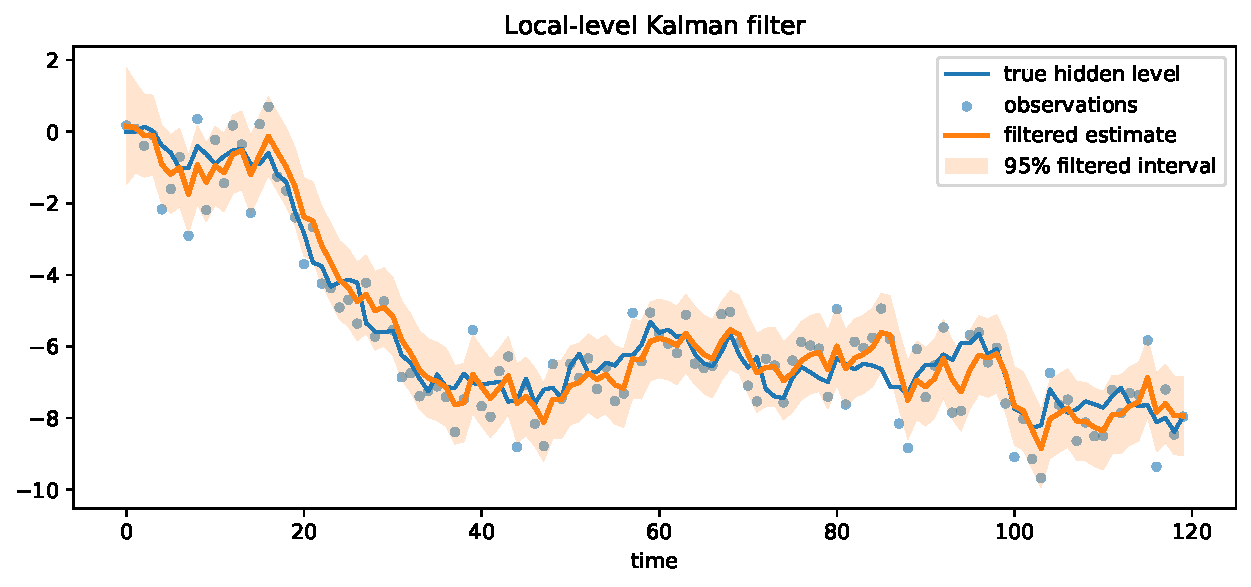
\includegraphics[keepaspectratio]{chapters/chapter-10-state-space-kalman-filtering_files/figure-pdf/py-ch10-local-level-from-scratch-output-1.pdf}}

}

\caption{Local-level Kalman filter implemented from scratch.}

\end{figure}%

The plot shows three different objects:

\begin{itemize}
\tightlist
\item
  the hidden level \(\mu_t\), which is not observed in real
  applications;
\item
  the noisy observations \(y_t\);
\item
  the filtered estimate \(m_t=E(\mu_t\mid\mathcal{D}_t)\).
\end{itemize}

\section{10.18 Python example: vector Kalman
filter}\label{python-example-vector-kalman-filter}

The next implementation handles a general linear Gaussian state-space
model.

\protect\phantomsection\label{py-ch10-general-kalman-function}
\begin{Shaded}
\begin{Highlighting}[]
\ImportTok{import}\NormalTok{ numpy }\ImportTok{as}\NormalTok{ np}

\KeywordTok{def}\NormalTok{ kalman\_filter(y, F, G, V, W, m0, C0):}
    \CommentTok{"""Kalman filter for a scalar{-}observation linear Gaussian state{-}space model.}

\CommentTok{    Parameters}
\CommentTok{    {-}{-}{-}{-}{-}{-}{-}{-}{-}{-}}
\CommentTok{    y : array, shape (n,)}
\CommentTok{        Observations. Missing values may be represented by np.nan.}
\CommentTok{    F : array, shape (d,)}
\CommentTok{        Observation vector; y\_t = F.T @ alpha\_t + v\_t.}
\CommentTok{    G : array, shape (d, d)}
\CommentTok{        State transition matrix.}
\CommentTok{    V : float}
\CommentTok{        Observation variance.}
\CommentTok{    W : array, shape (d, d)}
\CommentTok{        State innovation covariance.}
\CommentTok{    m0 : array, shape (d,)}
\CommentTok{        Initial state mean.}
\CommentTok{    C0 : array, shape (d, d)}
\CommentTok{        Initial state covariance.}

\CommentTok{    Returns}
\CommentTok{    {-}{-}{-}{-}{-}{-}{-}}
\CommentTok{    dict containing filtered means, covariances, forecasts, forecast variances,}
\CommentTok{    innovations, and Kalman gains.}
\CommentTok{    """}
\NormalTok{    y }\OperatorTok{=}\NormalTok{ np.asarray(y, dtype}\OperatorTok{=}\BuiltInTok{float}\NormalTok{)}
\NormalTok{    F }\OperatorTok{=}\NormalTok{ np.asarray(F, dtype}\OperatorTok{=}\BuiltInTok{float}\NormalTok{)}
\NormalTok{    G }\OperatorTok{=}\NormalTok{ np.asarray(G, dtype}\OperatorTok{=}\BuiltInTok{float}\NormalTok{)}
\NormalTok{    W }\OperatorTok{=}\NormalTok{ np.asarray(W, dtype}\OperatorTok{=}\BuiltInTok{float}\NormalTok{)}

\NormalTok{    n }\OperatorTok{=} \BuiltInTok{len}\NormalTok{(y)}
\NormalTok{    d }\OperatorTok{=} \BuiltInTok{len}\NormalTok{(F)}

\NormalTok{    m }\OperatorTok{=}\NormalTok{ np.zeros((n, d))}
\NormalTok{    C }\OperatorTok{=}\NormalTok{ np.zeros((n, d, d))}
\NormalTok{    a }\OperatorTok{=}\NormalTok{ np.zeros((n, d))}
\NormalTok{    R }\OperatorTok{=}\NormalTok{ np.zeros((n, d, d))}
\NormalTok{    forecast }\OperatorTok{=}\NormalTok{ np.zeros(n)}
\NormalTok{    Q }\OperatorTok{=}\NormalTok{ np.zeros(n)}
\NormalTok{    innovation }\OperatorTok{=}\NormalTok{ np.full(n, np.nan)}
\NormalTok{    gain }\OperatorTok{=}\NormalTok{ np.zeros((n, d))}

\NormalTok{    m\_prev }\OperatorTok{=}\NormalTok{ np.asarray(m0, dtype}\OperatorTok{=}\BuiltInTok{float}\NormalTok{)}
\NormalTok{    C\_prev }\OperatorTok{=}\NormalTok{ np.asarray(C0, dtype}\OperatorTok{=}\BuiltInTok{float}\NormalTok{)}

    \ControlFlowTok{for}\NormalTok{ t }\KeywordTok{in} \BuiltInTok{range}\NormalTok{(n):}
        \CommentTok{\# State prediction}
\NormalTok{        a[t] }\OperatorTok{=}\NormalTok{ G }\OperatorTok{@}\NormalTok{ m\_prev}
\NormalTok{        R[t] }\OperatorTok{=}\NormalTok{ G }\OperatorTok{@}\NormalTok{ C\_prev }\OperatorTok{@}\NormalTok{ G.T }\OperatorTok{+}\NormalTok{ W}

        \CommentTok{\# Observation forecast}
\NormalTok{        forecast[t] }\OperatorTok{=}\NormalTok{ F }\OperatorTok{@}\NormalTok{ a[t]}
\NormalTok{        Q[t] }\OperatorTok{=}\NormalTok{ F }\OperatorTok{@}\NormalTok{ R[t] }\OperatorTok{@}\NormalTok{ F }\OperatorTok{+}\NormalTok{ V}

        \ControlFlowTok{if}\NormalTok{ np.isnan(y[t]):}
            \CommentTok{\# Missing observation: prediction becomes filtering distribution}
\NormalTok{            m[t] }\OperatorTok{=}\NormalTok{ a[t]}
\NormalTok{            C[t] }\OperatorTok{=}\NormalTok{ R[t]}
        \ControlFlowTok{else}\NormalTok{:}
\NormalTok{            innovation[t] }\OperatorTok{=}\NormalTok{ y[t] }\OperatorTok{{-}}\NormalTok{ forecast[t]}
\NormalTok{            gain[t] }\OperatorTok{=}\NormalTok{ R[t] }\OperatorTok{@}\NormalTok{ F }\OperatorTok{/}\NormalTok{ Q[t]}
\NormalTok{            m[t] }\OperatorTok{=}\NormalTok{ a[t] }\OperatorTok{+}\NormalTok{ gain[t] }\OperatorTok{*}\NormalTok{ innovation[t]}
\NormalTok{            C[t] }\OperatorTok{=}\NormalTok{ R[t] }\OperatorTok{{-}}\NormalTok{ np.outer(gain[t], gain[t]) }\OperatorTok{*}\NormalTok{ Q[t]}

\NormalTok{        m\_prev, C\_prev }\OperatorTok{=}\NormalTok{ m[t], C[t]}

    \ControlFlowTok{return}\NormalTok{ \{}
        \StringTok{"m"}\NormalTok{: m, }\StringTok{"C"}\NormalTok{: C, }\StringTok{"a"}\NormalTok{: a, }\StringTok{"R"}\NormalTok{: R,}
        \StringTok{"forecast"}\NormalTok{: forecast, }\StringTok{"Q"}\NormalTok{: Q,}
        \StringTok{"innovation"}\NormalTok{: innovation, }\StringTok{"gain"}\NormalTok{: gain}
\NormalTok{    \}}
\end{Highlighting}
\end{Shaded}

\section{10.19 Python example: local-linear trend
model}\label{python-example-local-linear-trend-model}

Now we apply the vector filter to the local-linear trend model.

\protect\phantomsection\label{py-ch10-local-linear-trend}
\begin{Shaded}
\begin{Highlighting}[]
\NormalTok{rng }\OperatorTok{=}\NormalTok{ np.random.default\_rng(}\DecValTok{10}\NormalTok{)}
\NormalTok{n }\OperatorTok{=} \DecValTok{160}

\NormalTok{true\_level }\OperatorTok{=}\NormalTok{ np.zeros(n)}
\NormalTok{true\_slope }\OperatorTok{=}\NormalTok{ np.zeros(n)}
\NormalTok{y }\OperatorTok{=}\NormalTok{ np.zeros(n)}

\NormalTok{level\_noise\_var }\OperatorTok{=} \FloatTok{0.05}
\NormalTok{slope\_noise\_var }\OperatorTok{=} \FloatTok{0.005}
\NormalTok{obs\_noise\_var }\OperatorTok{=} \FloatTok{0.50}

\NormalTok{true\_level[}\DecValTok{0}\NormalTok{] }\OperatorTok{=} \FloatTok{2.0}
\NormalTok{true\_slope[}\DecValTok{0}\NormalTok{] }\OperatorTok{=} \FloatTok{0.04}

\ControlFlowTok{for}\NormalTok{ t }\KeywordTok{in} \BuiltInTok{range}\NormalTok{(}\DecValTok{1}\NormalTok{, n):}
\NormalTok{    true\_level[t] }\OperatorTok{=}\NormalTok{ true\_level[t}\OperatorTok{{-}}\DecValTok{1}\NormalTok{] }\OperatorTok{+}\NormalTok{ true\_slope[t}\OperatorTok{{-}}\DecValTok{1}\NormalTok{] }\OperatorTok{+}\NormalTok{ rng.normal(}\DecValTok{0}\NormalTok{, np.sqrt(level\_noise\_var))}
\NormalTok{    true\_slope[t] }\OperatorTok{=}\NormalTok{ true\_slope[t}\OperatorTok{{-}}\DecValTok{1}\NormalTok{] }\OperatorTok{+}\NormalTok{ rng.normal(}\DecValTok{0}\NormalTok{, np.sqrt(slope\_noise\_var))}

\NormalTok{y }\OperatorTok{=}\NormalTok{ true\_level }\OperatorTok{+}\NormalTok{ rng.normal(}\DecValTok{0}\NormalTok{, np.sqrt(obs\_noise\_var), size}\OperatorTok{=}\NormalTok{n)}

\NormalTok{F }\OperatorTok{=}\NormalTok{ np.array([}\FloatTok{1.0}\NormalTok{, }\FloatTok{0.0}\NormalTok{])}
\NormalTok{G }\OperatorTok{=}\NormalTok{ np.array([[}\FloatTok{1.0}\NormalTok{, }\FloatTok{1.0}\NormalTok{],}
\NormalTok{              [}\FloatTok{0.0}\NormalTok{, }\FloatTok{1.0}\NormalTok{]])}
\NormalTok{W }\OperatorTok{=}\NormalTok{ np.diag([level\_noise\_var, slope\_noise\_var])}
\NormalTok{V }\OperatorTok{=}\NormalTok{ obs\_noise\_var}
\NormalTok{m0 }\OperatorTok{=}\NormalTok{ np.array([}\FloatTok{0.0}\NormalTok{, }\FloatTok{0.0}\NormalTok{])}
\NormalTok{C0 }\OperatorTok{=}\NormalTok{ np.diag([}\FloatTok{10.0}\NormalTok{, }\FloatTok{1.0}\NormalTok{])}

\NormalTok{out }\OperatorTok{=}\NormalTok{ kalman\_filter(y, F, G, V, W, m0, C0)}
\NormalTok{filtered\_level }\OperatorTok{=}\NormalTok{ out[}\StringTok{"m"}\NormalTok{][:, }\DecValTok{0}\NormalTok{]}
\NormalTok{filtered\_slope }\OperatorTok{=}\NormalTok{ out[}\StringTok{"m"}\NormalTok{][:, }\DecValTok{1}\NormalTok{]}

\NormalTok{plt.figure(figsize}\OperatorTok{=}\NormalTok{(}\DecValTok{10}\NormalTok{, }\DecValTok{4}\NormalTok{))}
\NormalTok{plt.scatter(np.arange(n), y, s}\OperatorTok{=}\DecValTok{12}\NormalTok{, alpha}\OperatorTok{=}\FloatTok{0.5}\NormalTok{, label}\OperatorTok{=}\StringTok{"observed data"}\NormalTok{)}
\NormalTok{plt.plot(true\_level, label}\OperatorTok{=}\StringTok{"true level"}\NormalTok{)}
\NormalTok{plt.plot(filtered\_level, linewidth}\OperatorTok{=}\DecValTok{2}\NormalTok{, label}\OperatorTok{=}\StringTok{"filtered level"}\NormalTok{)}
\NormalTok{plt.title(}\StringTok{"Local{-}linear trend model"}\NormalTok{)}
\NormalTok{plt.xlabel(}\StringTok{"time"}\NormalTok{)}
\NormalTok{plt.legend()}
\NormalTok{plt.show()}

\NormalTok{plt.figure(figsize}\OperatorTok{=}\NormalTok{(}\DecValTok{10}\NormalTok{, }\DecValTok{3}\NormalTok{))}
\NormalTok{plt.plot(true\_slope, label}\OperatorTok{=}\StringTok{"true slope"}\NormalTok{)}
\NormalTok{plt.plot(filtered\_slope, linewidth}\OperatorTok{=}\DecValTok{2}\NormalTok{, label}\OperatorTok{=}\StringTok{"filtered slope"}\NormalTok{)}
\NormalTok{plt.title(}\StringTok{"Estimated dynamic slope"}\NormalTok{)}
\NormalTok{plt.xlabel(}\StringTok{"time"}\NormalTok{)}
\NormalTok{plt.legend()}
\NormalTok{plt.show()}
\end{Highlighting}
\end{Shaded}

\begin{figure}[H]

{\centering \pandocbounded{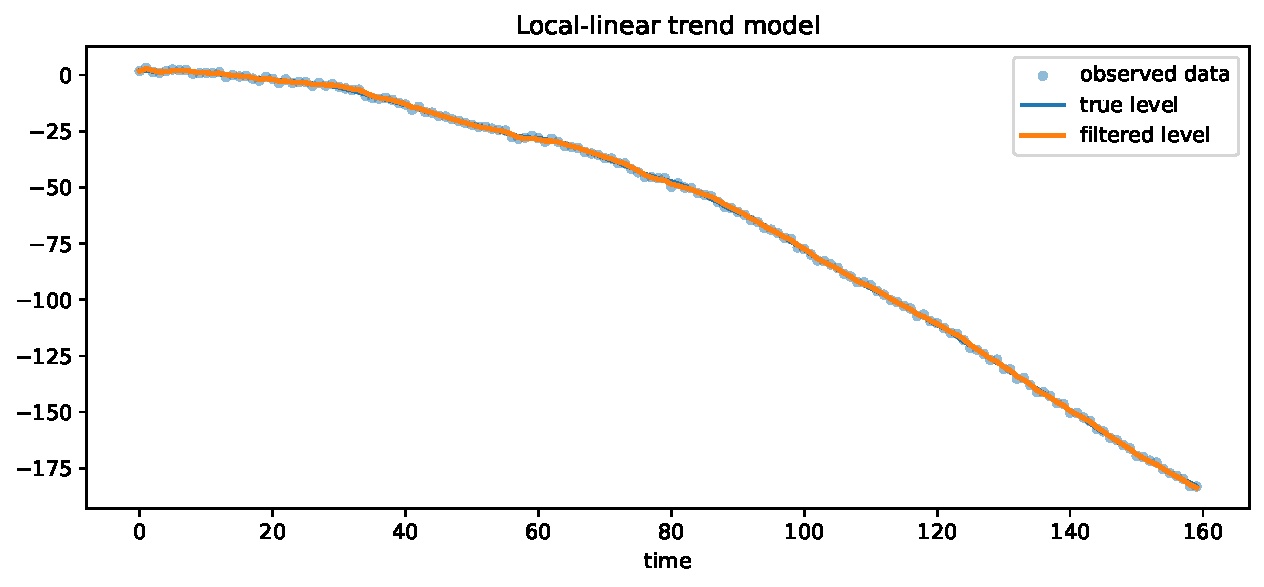
\includegraphics[keepaspectratio]{chapters/chapter-10-state-space-kalman-filtering_files/figure-pdf/py-ch10-local-linear-trend-output-1.pdf}}

}

\caption{Kalman filtering for a local-linear trend model.}

\end{figure}%

\pandocbounded{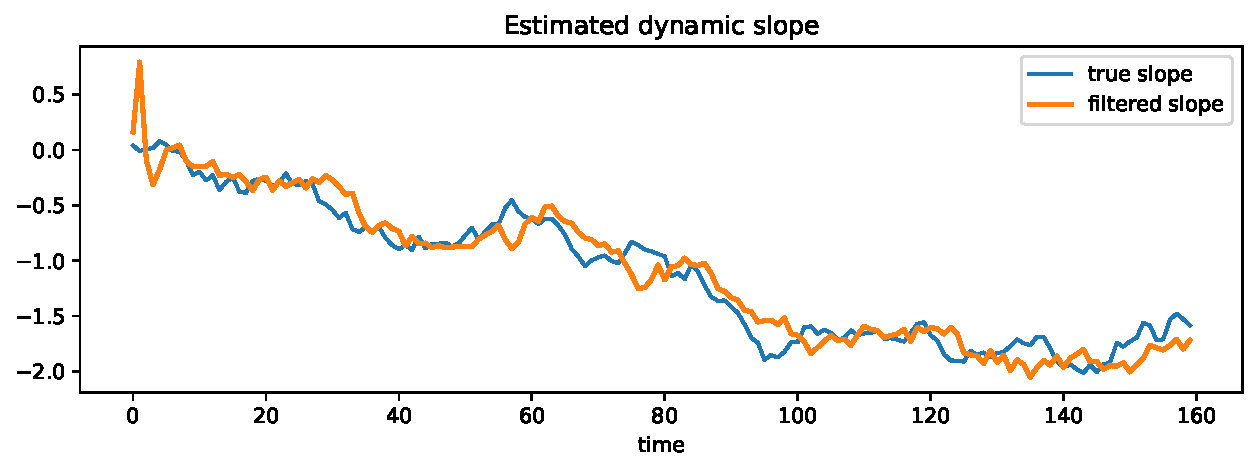
\includegraphics[keepaspectratio]{chapters/chapter-10-state-space-kalman-filtering_files/figure-pdf/py-ch10-local-linear-trend-output-2.pdf}}

This example shows why state-space models are useful for nonstationary
data. Rather than differencing the series and modeling the transformed
data, we explicitly model the evolving level and slope.

\section{10.20 Python example: missing
observations}\label{python-example-missing-observations}

The same filtering function can handle missing values represented by
\texttt{np.nan}.

\begin{Shaded}
\begin{Highlighting}[]
\NormalTok{rng }\OperatorTok{=}\NormalTok{ np.random.default\_rng(}\DecValTok{12}\NormalTok{)}
\NormalTok{y\_missing }\OperatorTok{=}\NormalTok{ y.copy()}
\NormalTok{missing\_index }\OperatorTok{=}\NormalTok{ np.r\_[}\DecValTok{40}\NormalTok{:}\DecValTok{58}\NormalTok{, }\DecValTok{100}\NormalTok{:}\DecValTok{112}\NormalTok{]}
\NormalTok{y\_missing[missing\_index] }\OperatorTok{=}\NormalTok{ np.nan}

\NormalTok{out\_missing }\OperatorTok{=}\NormalTok{ kalman\_filter(y\_missing, F, G, V, W, m0, C0)}
\NormalTok{filtered\_missing }\OperatorTok{=}\NormalTok{ out\_missing[}\StringTok{"m"}\NormalTok{][:, }\DecValTok{0}\NormalTok{]}
\NormalTok{C\_level }\OperatorTok{=}\NormalTok{ out\_missing[}\StringTok{"C"}\NormalTok{][:, }\DecValTok{0}\NormalTok{, }\DecValTok{0}\NormalTok{]}

\NormalTok{plt.figure(figsize}\OperatorTok{=}\NormalTok{(}\DecValTok{10}\NormalTok{, }\DecValTok{4}\NormalTok{))}
\NormalTok{plt.scatter(np.arange(n), y\_missing, s}\OperatorTok{=}\DecValTok{14}\NormalTok{, alpha}\OperatorTok{=}\FloatTok{0.6}\NormalTok{, label}\OperatorTok{=}\StringTok{"observed data with gaps"}\NormalTok{)}
\NormalTok{plt.plot(true\_level, label}\OperatorTok{=}\StringTok{"true level"}\NormalTok{)}
\NormalTok{plt.plot(filtered\_missing, linewidth}\OperatorTok{=}\DecValTok{2}\NormalTok{, label}\OperatorTok{=}\StringTok{"filtered level"}\NormalTok{)}
\NormalTok{plt.fill\_between(}
\NormalTok{    np.arange(n),}
\NormalTok{    filtered\_missing }\OperatorTok{{-}} \FloatTok{1.96} \OperatorTok{*}\NormalTok{ np.sqrt(C\_level),}
\NormalTok{    filtered\_missing }\OperatorTok{+} \FloatTok{1.96} \OperatorTok{*}\NormalTok{ np.sqrt(C\_level),}
\NormalTok{    alpha}\OperatorTok{=}\FloatTok{0.2}\NormalTok{,}
\NormalTok{    label}\OperatorTok{=}\StringTok{"95}\SpecialCharTok{\% s}\StringTok{tate interval"}
\NormalTok{)}
\NormalTok{plt.axvspan(}\DecValTok{40}\NormalTok{, }\DecValTok{57}\NormalTok{, alpha}\OperatorTok{=}\FloatTok{0.1}\NormalTok{)}
\NormalTok{plt.axvspan(}\DecValTok{100}\NormalTok{, }\DecValTok{111}\NormalTok{, alpha}\OperatorTok{=}\FloatTok{0.1}\NormalTok{)}
\NormalTok{plt.title(}\StringTok{"State{-}space filtering naturally handles missing observations"}\NormalTok{)}
\NormalTok{plt.xlabel(}\StringTok{"time"}\NormalTok{)}
\NormalTok{plt.legend()}
\NormalTok{plt.show()}
\end{Highlighting}
\end{Shaded}

\begin{figure}[H]

{\centering \pandocbounded{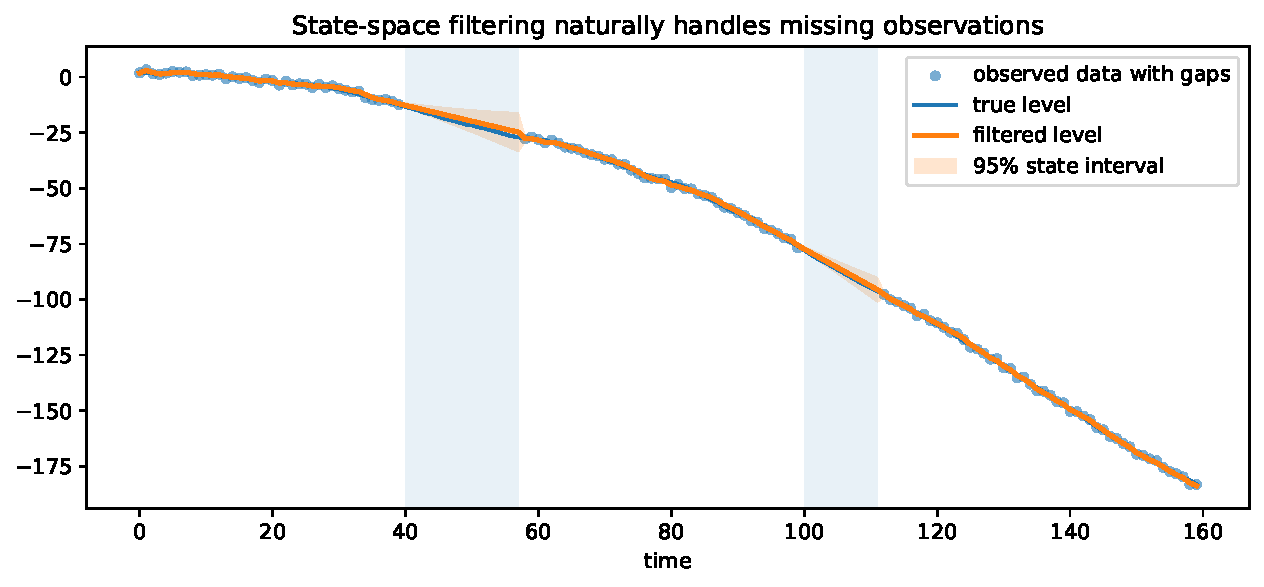
\includegraphics[keepaspectratio]{chapters/chapter-10-state-space-kalman-filtering_files/figure-pdf/py-ch10-missing-values-output-1.pdf}}

}

\caption{Kalman filtering with missing observations.}

\end{figure}%

During gaps, the filter still evolves the state forward, but uncertainty
increases because no observations are available for correction.

\section{10.21 Python example: log
likelihood}\label{python-example-log-likelihood}

We can estimate model parameters by maximizing the Kalman filter log
likelihood. The function below evaluates the log likelihood for fixed
parameters.

\begin{Shaded}
\begin{Highlighting}[]
\KeywordTok{def}\NormalTok{ kalman\_loglik(y, F, G, V, W, m0, C0):}
\NormalTok{    out }\OperatorTok{=}\NormalTok{ kalman\_filter(y, F, G, V, W, m0, C0)}
\NormalTok{    e }\OperatorTok{=}\NormalTok{ out[}\StringTok{"innovation"}\NormalTok{]}
\NormalTok{    Q }\OperatorTok{=}\NormalTok{ out[}\StringTok{"Q"}\NormalTok{]}
\NormalTok{    observed }\OperatorTok{=} \OperatorTok{\textasciitilde{}}\NormalTok{np.isnan(y)}
\NormalTok{    ll }\OperatorTok{=} \OperatorTok{{-}}\FloatTok{0.5} \OperatorTok{*}\NormalTok{ np.}\BuiltInTok{sum}\NormalTok{(}
\NormalTok{        np.log(}\DecValTok{2} \OperatorTok{*}\NormalTok{ np.pi) }\OperatorTok{+}\NormalTok{ np.log(Q[observed]) }\OperatorTok{+}\NormalTok{ e[observed] }\OperatorTok{**} \DecValTok{2} \OperatorTok{/}\NormalTok{ Q[observed]}
\NormalTok{    )}
    \ControlFlowTok{return}\NormalTok{ ll}

\NormalTok{candidate\_values }\OperatorTok{=}\NormalTok{ np.linspace(}\FloatTok{0.05}\NormalTok{, }\FloatTok{2.0}\NormalTok{, }\DecValTok{60}\NormalTok{)}
\NormalTok{loglik\_values }\OperatorTok{=}\NormalTok{ []}

\ControlFlowTok{for}\NormalTok{ V\_candidate }\KeywordTok{in}\NormalTok{ candidate\_values:}
\NormalTok{    ll }\OperatorTok{=}\NormalTok{ kalman\_loglik(y, F, G, V\_candidate, W, m0, C0)}
\NormalTok{    loglik\_values.append(ll)}

\NormalTok{best\_V }\OperatorTok{=}\NormalTok{ candidate\_values[np.argmax(loglik\_values)]}
\BuiltInTok{print}\NormalTok{(}\SpecialStringTok{f"Best observation variance on grid: }\SpecialCharTok{\{}\NormalTok{best\_V}\SpecialCharTok{:.3f\}}\SpecialStringTok{"}\NormalTok{)}

\NormalTok{plt.figure(figsize}\OperatorTok{=}\NormalTok{(}\DecValTok{8}\NormalTok{, }\DecValTok{4}\NormalTok{))}
\NormalTok{plt.plot(candidate\_values, loglik\_values)}
\NormalTok{plt.axvline(best\_V, linestyle}\OperatorTok{=}\StringTok{"{-}{-}"}\NormalTok{)}
\NormalTok{plt.xlabel(}\StringTok{"candidate observation variance V"}\NormalTok{)}
\NormalTok{plt.ylabel(}\StringTok{"Kalman log likelihood"}\NormalTok{)}
\NormalTok{plt.title(}\StringTok{"Grid likelihood for observation noise variance"}\NormalTok{)}
\NormalTok{plt.show()}
\end{Highlighting}
\end{Shaded}

\begin{verbatim}
Best observation variance on grid: 0.546
\end{verbatim}

\pandocbounded{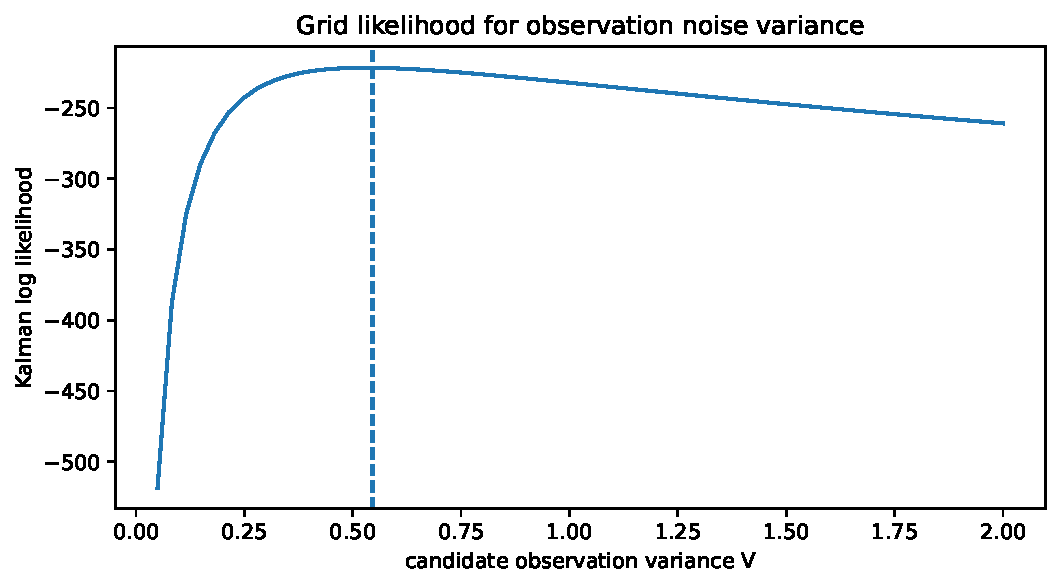
\includegraphics[keepaspectratio]{chapters/chapter-10-state-space-kalman-filtering_files/figure-pdf/py-ch10-loglikelihood-output-2.pdf}}

This is not a full maximum-likelihood routine, but it illustrates the
principle. In practice, we often optimize over multiple transformed
parameters using numerical optimization.

\section{10.22 Forecasting with the local-linear
model}\label{forecasting-with-the-local-linear-model}

The following code produces multi-step forecasts from the filtered
distribution at the end of the sample.

\begin{Shaded}
\begin{Highlighting}[]
\NormalTok{h }\OperatorTok{=} \DecValTok{30}
\NormalTok{last\_m }\OperatorTok{=}\NormalTok{ out[}\StringTok{"m"}\NormalTok{][}\OperatorTok{{-}}\DecValTok{1}\NormalTok{]}
\NormalTok{last\_C }\OperatorTok{=}\NormalTok{ out[}\StringTok{"C"}\NormalTok{][}\OperatorTok{{-}}\DecValTok{1}\NormalTok{]}

\NormalTok{forecast\_mean }\OperatorTok{=}\NormalTok{ np.zeros(h)}
\NormalTok{forecast\_var }\OperatorTok{=}\NormalTok{ np.zeros(h)}

\NormalTok{m\_h }\OperatorTok{=}\NormalTok{ last\_m.copy()}
\NormalTok{C\_h }\OperatorTok{=}\NormalTok{ last\_C.copy()}

\ControlFlowTok{for}\NormalTok{ j }\KeywordTok{in} \BuiltInTok{range}\NormalTok{(h):}
\NormalTok{    m\_h }\OperatorTok{=}\NormalTok{ G }\OperatorTok{@}\NormalTok{ m\_h}
\NormalTok{    C\_h }\OperatorTok{=}\NormalTok{ G }\OperatorTok{@}\NormalTok{ C\_h }\OperatorTok{@}\NormalTok{ G.T }\OperatorTok{+}\NormalTok{ W}
\NormalTok{    forecast\_mean[j] }\OperatorTok{=}\NormalTok{ F }\OperatorTok{@}\NormalTok{ m\_h}
\NormalTok{    forecast\_var[j] }\OperatorTok{=}\NormalTok{ F }\OperatorTok{@}\NormalTok{ C\_h }\OperatorTok{@}\NormalTok{ F }\OperatorTok{+}\NormalTok{ V}

\NormalTok{future\_time }\OperatorTok{=}\NormalTok{ np.arange(n, n }\OperatorTok{+}\NormalTok{ h)}

\NormalTok{plt.figure(figsize}\OperatorTok{=}\NormalTok{(}\DecValTok{10}\NormalTok{, }\DecValTok{4}\NormalTok{))}
\NormalTok{plt.plot(np.arange(n), y, label}\OperatorTok{=}\StringTok{"observed"}\NormalTok{)}
\NormalTok{plt.plot(future\_time, forecast\_mean, label}\OperatorTok{=}\StringTok{"forecast mean"}\NormalTok{)}
\NormalTok{plt.fill\_between(}
\NormalTok{    future\_time,}
\NormalTok{    forecast\_mean }\OperatorTok{{-}} \FloatTok{1.96} \OperatorTok{*}\NormalTok{ np.sqrt(forecast\_var),}
\NormalTok{    forecast\_mean }\OperatorTok{+} \FloatTok{1.96} \OperatorTok{*}\NormalTok{ np.sqrt(forecast\_var),}
\NormalTok{    alpha}\OperatorTok{=}\FloatTok{0.2}\NormalTok{,}
\NormalTok{    label}\OperatorTok{=}\StringTok{"95}\SpecialCharTok{\% f}\StringTok{orecast interval"}
\NormalTok{)}
\NormalTok{plt.axvline(n }\OperatorTok{{-}} \DecValTok{1}\NormalTok{, linestyle}\OperatorTok{=}\StringTok{"{-}{-}"}\NormalTok{)}
\NormalTok{plt.title(}\StringTok{"State{-}space forecast"}\NormalTok{)}
\NormalTok{plt.xlabel(}\StringTok{"time"}\NormalTok{)}
\NormalTok{plt.legend()}
\NormalTok{plt.show()}
\end{Highlighting}
\end{Shaded}

\begin{figure}[H]

{\centering \pandocbounded{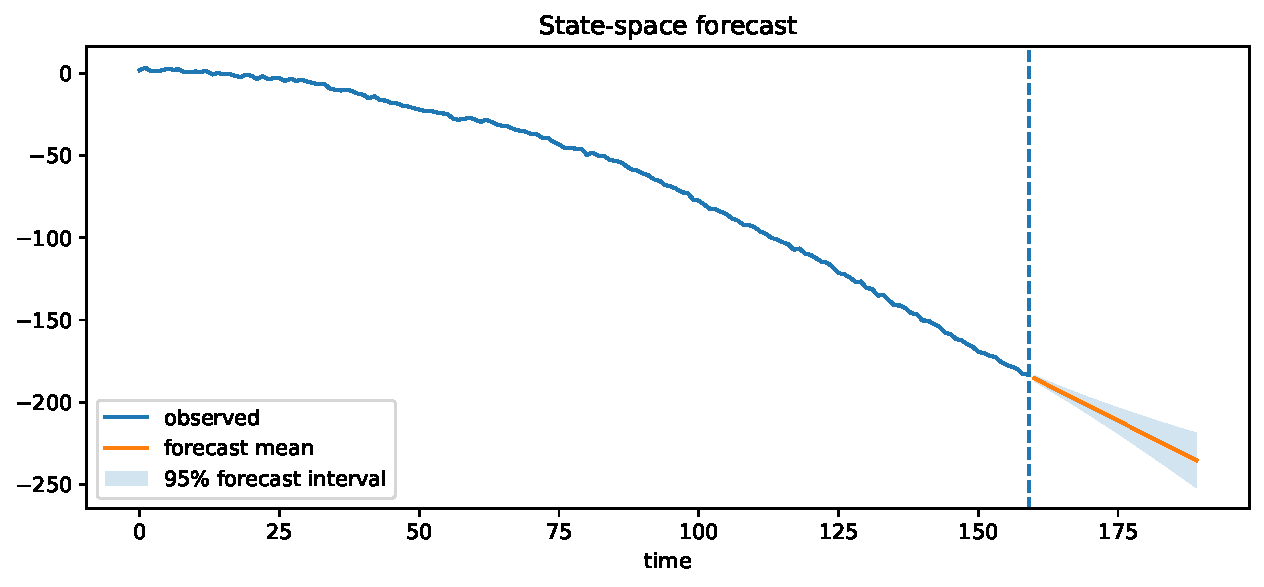
\includegraphics[keepaspectratio]{chapters/chapter-10-state-space-kalman-filtering_files/figure-pdf/py-ch10-state-space-forecast-output-1.pdf}}

}

\caption{Multi-step forecasts from a local-linear state-space model.}

\end{figure}%

The forecast interval widens with horizon because state uncertainty
accumulates over time.

\section{10.23 State-space models and
ARIMA}\label{state-space-models-and-arima}

Many ARIMA models have state-space representations. This matters for at
least three reasons.

First, it allows ARIMA models to be fitted by Kalman filtering. Second,
it gives a natural way to compute likelihoods and handle missing values.
Third, it shows how ARIMA belongs to a larger family of dynamic
hidden-state models.

For example, the random walk plus noise model is

\[
\mu_t=\mu_{t-1}+w_t,
\qquad
 y_t=\mu_t+v_t.
\]

This is close in spirit to an integrated model, but it separates
\textbf{state noise} \(w_t\) from \textbf{observation noise} \(v_t\). In
many scientific and engineering settings, this distinction is essential.

The state-space view is especially useful when we want to combine:

\[
\text{trend} + \text{seasonality} + \text{regression} + \text{ARMA errors} + \text{missing data}.
\]

\section{10.24 Dynamic regression}\label{dynamic-regression}

A static regression model is

\[
y_t=\mathbf{x}_t^\top\boldsymbol{\beta}+\epsilon_t.
\]

A dynamic regression model allows coefficients to change over time:

\[
y_t=\mathbf{x}_t^\top\boldsymbol{\beta}_t+v_t,
\]

\[
\boldsymbol{\beta}_t=\boldsymbol{\beta}_{t-1}+\mathbf{w}_t.
\]

This is a state-space model with state
\(\boldsymbol{\alpha}_t=\boldsymbol{\beta}_t\) and observation vector
\(\mathbf{F}_t=\mathbf{x}_t\).

Dynamic regression is useful when the effect of a predictor is not
constant. Examples include:

\begin{itemize}
\tightlist
\item
  changing price sensitivity in retail demand;
\item
  time-varying market beta in finance;
\item
  changing intervention effects in public-health data;
\item
  evolving relationship between weather and energy demand.
\end{itemize}

\section{10.25 State-space models and modern sequence
learning}\label{state-space-models-and-modern-sequence-learning}

State-space models provide a bridge from classical time-series theory to
modern AI.

\subsection{Connection to RNNs}\label{connection-to-rnns}

A recurrent neural network has a hidden state update

\[
\mathbf{h}_t=\sigma(\mathbf{A}\mathbf{h}_{t-1}+\mathbf{B}\mathbf{x}_t+\mathbf{b}).
\]

A linear Gaussian state-space model has a hidden state update

\[
\boldsymbol{\alpha}_t=\mathbf{G}\boldsymbol{\alpha}_{t-1}+\mathbf{w}_t.
\]

Both models maintain a hidden summary of the past. The state-space model
is probabilistic and interpretable. The RNN is nonlinear and highly
expressive.

\subsection{Connection to HMMs}\label{connection-to-hmms}

A hidden Markov model also has hidden states, but the states are usually
discrete:

\[
S_t\in\{1,2,\ldots,K\}.
\]

The Kalman filter is the Gaussian continuous-state analogue of recursive
filtering for hidden Markov models.

\subsection{Connection to attention
models}\label{connection-to-attention-models}

Attention models do not compress the past into a single low-dimensional
state in the same way. Instead, they learn to attend to many past
positions. However, state-space ideas remain important in modern
long-sequence modeling because they offer efficient recurrent updates.

\begin{tcolorbox}[enhanced jigsaw, arc=.35mm, bottomrule=.15mm, bottomtitle=1mm, breakable, colback=white, colbacktitle=quarto-callout-important-color!10!white, colframe=quarto-callout-important-color-frame, coltitle=black, left=2mm, leftrule=.75mm, opacityback=0, opacitybacktitle=0.6, rightrule=.15mm, title=\textcolor{quarto-callout-important-color}{\faExclamation}\hspace{0.5em}{AI perspective}, titlerule=0mm, toprule=.15mm, toptitle=1mm]

A state-space model is an interpretable probabilistic memory system.
RNNs, gated models, and transformers are more flexible sequence models,
but they inherit the same core question: how should past information be
stored and used for prediction?

\end{tcolorbox}

\section{10.26 AI-assisted modeling
component}\label{ai-assisted-modeling-component}

AI tools can help with state-space modeling, but recursion and matrix
notation are easy places for AI-generated code to make subtle mistakes.
Use AI as a critic and debugging assistant, not as an authority.

\subsection{Prompt 1: Dimension audit}\label{prompt-1-dimension-audit}

\begin{quote}
I am implementing a Kalman filter with state dimension \(d=2\). My
observation vector is \(F=[1,0]^T\), transition matrix is
\(G=\begin{bmatrix}1&1\\0&1\end{bmatrix}\), and state covariance is
\(C_t\). Check the dimensions of every term in the prediction, forecast,
gain, and update equations. Do not change the model; only check
dimensions.
\end{quote}

\subsection{Prompt 2: Model
interpretation}\label{prompt-2-model-interpretation}

\begin{quote}
Explain the difference between a local-level model and a local-linear
trend model. Give one example where the local-level model is sufficient
and one example where the local-linear trend model is more appropriate.
\end{quote}

\subsection{Prompt 3: Debugging recursive
code}\label{prompt-3-debugging-recursive-code}

\begin{quote}
Here is my Kalman filter function. Identify possible indexing,
covariance-update, missing-data, and numerical-stability issues. Do not
rewrite the entire function unless necessary. Explain each issue
mathematically.
\end{quote}

\subsection{Prompt 4: Forecast
uncertainty}\label{prompt-4-forecast-uncertainty}

\begin{quote}
Why does the state-space forecast interval widen as the horizon
increases? Explain using the formula for \(R_{t+h|t}\).
\end{quote}

\subsection{Verification checklist for AI
answers}\label{verification-checklist-for-ai-answers}

\begin{enumerate}
\def\labelenumi{\arabic{enumi}.}
\tightlist
\item
  Are the dimensions correct?
\item
  Are covariance matrices symmetric and positive semidefinite?
\item
  Is \(Q_t\) positive?
\item
  Are missing observations skipped rather than imputed without
  justification?
\item
  Are filtering and smoothing clearly distinguished?
\item
  Are forecast intervals based on observation uncertainty, not only
  state uncertainty?
\end{enumerate}

\section{10.27 Common mistakes}\label{common-mistakes-9}

\subsection{Mistake 1: Confusing state noise with observation
noise}\label{mistake-1-confusing-state-noise-with-observation-noise}

In

\[
y_t=\mu_t+v_t,
\qquad
\mu_t=\mu_{t-1}+w_t,
\]

\(v_t\) is measurement noise and \(w_t\) is state evolution noise.
Increasing \(V\) makes observations less reliable. Increasing \(W\)
makes the hidden state more flexible.

\subsection{\texorpdfstring{Mistake 2: Updating when \(y_t\) is
missing}{Mistake 2: Updating when y\_t is missing}}\label{mistake-2-updating-when-y_t-is-missing}

If \(y_t\) is missing, do not compute an innovation using an imputed
value unless the imputation is explicitly part of the model. The
standard filter simply skips the update.

\subsection{Mistake 3: Using only state variance for forecast
intervals}\label{mistake-3-using-only-state-variance-for-forecast-intervals}

Forecast intervals for future observations must include observation
variance \(V\):

\[
Q_{t+h|t}=\mathbf{F}^\top\mathbf{R}_{t+h|t}\mathbf{F}+V.
\]

\subsection{Mistake 4: Forgetting covariance
propagation}\label{mistake-4-forgetting-covariance-propagation}

The forecast mean evolves through \(\mathbf{G}\), but so does
uncertainty:

\[
\mathbf{R}_t=\mathbf{G}\mathbf{C}_{t-1}\mathbf{G}^\top+\mathbf{W}.
\]

\subsection{Mistake 5: Confusing filtering with
smoothing}\label{mistake-5-confusing-filtering-with-smoothing}

Filtering uses only present and past data. Smoothing uses future data as
well. A smoothed estimate usually looks better, but it is not available
in real-time forecasting.

\section{10.28 Exercises}\label{exercises-9}

\subsection{Exercise 1: Scalar Kalman
gain}\label{exercise-1-scalar-kalman-gain}

For the local-level model, show that the Kalman gain is

\[
A_t=\frac{R_t}{R_t+V}.
\]

Explain what happens to \(A_t\) as \(V\to\infty\) and as \(V\to 0\).

\subsection{Exercise 2: Local-level
recursions}\label{exercise-2-local-level-recursions}

Starting from

\[
\mu_t=\mu_{t-1}+w_t,
\qquad
 y_t=\mu_t+v_t,
\]

derive all scalar Kalman filter equations.

\subsection{Exercise 3: Matrix
dimensions}\label{exercise-3-matrix-dimensions}

Let

\[
\mathbf{F}=\begin{bmatrix}1\\0\end{bmatrix},
\qquad
\mathbf{G}=\begin{bmatrix}1&1\\0&1\end{bmatrix}.
\]

List the dimensions of \(\mathbf{a}_t\), \(\mathbf{R}_t\), \(f_t\),
\(Q_t\), \(e_t\), \(\mathbf{A}_t\), \(\mathbf{m}_t\), and
\(\mathbf{C}_t\).

\subsection{Exercise 4: Missing
observation}\label{exercise-4-missing-observation}

Suppose \(y_t\) is missing. Write the filtering equations for time
\(t\). Explain why the covariance usually increases relative to time
\(t-1\).

\subsection{Exercise 5: Forecast
variance}\label{exercise-5-forecast-variance}

For a local-level model with \(G=1\), show that

\[
R_{t+h|t}=C_t+hW.
\]

Then write the \(h\)-step observation forecast variance.

\subsection{Exercise 6: Local-linear trend
simulation}\label{exercise-6-local-linear-trend-simulation}

Simulate a local-linear trend model and fit it using the Kalman filter.
Compare the filtered slope estimate with the true slope.

\subsection{Exercise 7: State-space versus
ARIMA}\label{exercise-7-state-space-versus-arima}

Write a short explanation comparing an ARIMA model and a local-linear
trend state-space model for a trending nonstationary series.

\subsection{Exercise 8: AI critique}\label{exercise-8-ai-critique}

Ask an AI tool to generate a Kalman filter for the local-level model.
Then audit the code for dimension consistency, missing-data handling,
and the correct covariance update.

\section{10.29 Mini project: noisy sensor
tracking}\label{mini-project-noisy-sensor-tracking}

Choose or simulate a time series representing a noisy sensor
measurement. Examples include position tracking, temperature monitoring,
demand level, or a latent biological signal.

Your project should include:

\begin{enumerate}
\def\labelenumi{\arabic{enumi}.}
\tightlist
\item
  a clear state-space model specification;
\item
  simulation or data description;
\item
  implementation of the Kalman filter;
\item
  plots of observations, filtered state estimates, and uncertainty
  bands;
\item
  a missing-data experiment;
\item
  multi-step forecasts with prediction intervals;
\item
  an AI-assisted debugging appendix describing how you checked the
  recursive equations.
\end{enumerate}

\section{10.30 Chapter checklist}\label{chapter-checklist-7}

You should now be able to:

\begin{itemize}
\tightlist
\item[$\square$]
  define a linear Gaussian state-space model;
\item[$\square$]
  identify the hidden state, observation equation, and state equation;
\item[$\square$]
  derive the Kalman prediction step;
\item[$\square$]
  derive the Kalman forecast step;
\item[$\square$]
  derive the Kalman update step;
\item[$\square$]
  explain the Kalman gain;
\item[$\square$]
  implement the local-level Kalman filter from scratch;
\item[$\square$]
  implement a vector Kalman filter;
\item[$\square$]
  handle missing observations;
\item[$\square$]
  compute multi-step forecast intervals;
\item[$\square$]
  distinguish filtering, smoothing, and forecasting;
\item[$\square$]
  explain how state-space models connect to ARIMA, HMMs, and RNNs.
\end{itemize}

\section{10.31 Key takeaways}\label{key-takeaways-1}

A state-space model separates a time series into hidden dynamic
structure and noisy observations. The Kalman filter provides an exact
recursive solution for linear Gaussian models. It updates a predicted
state using the new observation's innovation, weighted by the Kalman
gain. This gives a mathematically transparent framework for filtering,
forecasting, smoothing, likelihood evaluation, missing-data handling,
dynamic regression, and modern sequence-learning connections.

\chapter{Hidden Markov Models and Regime
Switching}\label{hidden-markov-models-and-regime-switching}

\textbf{Part III. Nonstationary and Seasonal Models}\\
\textbf{Chapter goal:} learn how to model sequence data whose behavior
changes across unobserved states. We develop hidden Markov models,
forward filtering, backward smoothing, Viterbi decoding, Baum--Welch
estimation, Gaussian emissions, regime-switching time series,
forecasting, diagnostics, and AI-assisted model critique.

\section{Learning objectives}\label{learning-objectives-10}

After studying this chapter, you should be able to:

\begin{enumerate}
\def\labelenumi{\arabic{enumi}.}
\tightlist
\item
  explain why hidden regimes are useful for time series and sequence
  data;
\item
  distinguish an observed sequence from an unobserved state sequence;
\item
  write the joint probability of a hidden Markov model;
\item
  implement the forward algorithm for likelihood evaluation;
\item
  implement backward smoothing probabilities;
\item
  use the Viterbi algorithm to decode the most likely hidden path;
\item
  describe the Baum--Welch algorithm as an expectation--maximization
  method;
\item
  fit and interpret a Gaussian HMM for regime-switching time series;
\item
  compare HMMs with Kalman filters, ARIMA models, and recurrent neural
  networks;
\item
  use AI tools to audit assumptions, code, diagnostics, and
  interpretation without outsourcing mathematical verification.
\end{enumerate}

\section{11.1 Why hidden regimes?}\label{why-hidden-regimes}

Many time series do not behave the same way at all times. A financial
return series may alternate between calm and volatile periods. A machine
sensor may switch between normal, warning, and failure modes. A
biological signal may move between resting and active states. A user's
behavior sequence may switch between browsing, comparing, and purchasing
modes.

A single stationary ARMA model may be too rigid for such data. Instead
of assuming one global dependence structure, we allow the sequence to
move through hidden regimes:

\[
S_t \in \{1,2,\ldots,K\},
\]

where \(S_t\) is not directly observed. The observed value \(Y_t\) is
generated from a distribution that depends on \(S_t\).

For example, a two-regime return model might be

\[
Y_t \mid S_t=1 \sim N(0,\sigma_1^2),
\qquad
Y_t \mid S_t=2 \sim N(0,\sigma_2^2),
\]

where \(\sigma_2^2 \gg \sigma_1^2\). State 1 represents a low-volatility
regime and state 2 represents a high-volatility regime.

\begin{tcolorbox}[enhanced jigsaw, arc=.35mm, bottomrule=.15mm, bottomtitle=1mm, breakable, colback=white, colbacktitle=quarto-callout-note-color!10!white, colframe=quarto-callout-note-color-frame, coltitle=black, left=2mm, leftrule=.75mm, opacityback=0, opacitybacktitle=0.6, rightrule=.15mm, title=\textcolor{quarto-callout-note-color}{\faInfo}\hspace{0.5em}{The hidden-state viewpoint}, titlerule=0mm, toprule=.15mm, toptitle=1mm]

An HMM separates two questions:

\begin{enumerate}
\def\labelenumi{\arabic{enumi}.}
\tightlist
\item
  \textbf{State dynamics:} how the hidden regime evolves over time.
\item
  \textbf{Emission model:} how the observed data are generated once the
  state is known.
\end{enumerate}

This is the discrete-state analogue of the state-space model from
Chapter 10.

\end{tcolorbox}

\section{11.2 Markov chains for latent
states}\label{markov-chains-for-latent-states}

The hidden state sequence \(S_1,S_2,\ldots,S_T\) is usually modeled as a
Markov chain:

\[
P(S_t=j\mid S_{1:t-1})=P(S_t=j\mid S_{t-1}).
\]

For \(K\) states, define the transition matrix

\[
\mathbf{A}=(a_{ij})_{i,j=1}^K,
\qquad
 a_{ij}=P(S_t=j\mid S_{t-1}=i).
\]

Each row of \(\mathbf{A}\) is a probability vector:

\[
a_{ij}\geq 0,
\qquad
\sum_{j=1}^K a_{ij}=1.
\]

The initial distribution is

\[
\boldsymbol{\pi}=(\pi_1,\ldots,\pi_K),
\qquad
\pi_j=P(S_1=j).
\]

For a two-state model,

\[
\mathbf{A}=\begin{bmatrix}
p_{11} & 1-p_{11}\\
1-p_{22} & p_{22}
\end{bmatrix}.
\]

Large values of \(p_{11}\) and \(p_{22}\) make regimes persistent. In
applications, persistence is often important: volatility clusters,
machines remain in a degraded state for some time, and users stay in a
behavioral mode for several steps.

\subsection{Expected regime duration}\label{expected-regime-duration}

If state \(j\) has self-transition probability \(a_{jj}\), then the
duration spent in state \(j\) before leaving is geometrically
distributed:

\[
P(D_j=d)=a_{jj}^{d-1}(1-a_{jj}),
\qquad d=1,2,\ldots.
\]

Therefore,

\[
E[D_j]=\frac{1}{1-a_{jj}}.
\]

This gives a useful interpretation of transition probabilities. If
\(a_{jj}=0.95\), the expected duration is \(20\) time steps.

\section{11.3 Hidden Markov model
definition}\label{hidden-markov-model-definition}

A hidden Markov model has three pieces:

\[
\lambda=(\boldsymbol{\pi},\mathbf{A},\mathbf{B}),
\]

where \(\boldsymbol{\pi}\) is the initial distribution, \(\mathbf{A}\)
is the transition matrix, and \(\mathbf{B}\) describes the emission
distributions.

For observations \(Y_1,\ldots,Y_T\), the model assumptions are:

\begin{enumerate}
\def\labelenumi{\arabic{enumi}.}
\tightlist
\item
  The hidden states form a Markov chain:
\end{enumerate}

\[
P(S_t\mid S_{1:t-1})=P(S_t\mid S_{t-1}).
\]

\begin{enumerate}
\def\labelenumi{\arabic{enumi}.}
\setcounter{enumi}{1}
\tightlist
\item
  Given the current state, the current observation is conditionally
  independent of all other variables:
\end{enumerate}

\[
P(Y_t\mid S_{1:T},Y_{1:t-1},Y_{t+1:T})=P(Y_t\mid S_t).
\]

\begin{enumerate}
\def\labelenumi{\arabic{enumi}.}
\setcounter{enumi}{2}
\tightlist
\item
  The emission density or probability mass function for state \(j\) is
\end{enumerate}

\[
b_j(y)=p(y\mid S_t=j).
\]

The joint probability of one hidden path \(s_{1:T}\) and observed
sequence \(y_{1:T}\) is

\[
P(s_{1:T},y_{1:T})
=\pi_{s_1} b_{s_1}(y_1)
\prod_{t=2}^T a_{s_{t-1},s_t} b_{s_t}(y_t).
\]

This single formula is the source of the main algorithms in this
chapter.

\begin{tcolorbox}[enhanced jigsaw, arc=.35mm, bottomrule=.15mm, bottomtitle=1mm, breakable, colback=white, colbacktitle=quarto-callout-tip-color!10!white, colframe=quarto-callout-tip-color-frame, coltitle=black, left=2mm, leftrule=.75mm, opacityback=0, opacitybacktitle=0.6, rightrule=.15mm, title=\textcolor{quarto-callout-tip-color}{\faLightbulb}\hspace{0.5em}{HMMs for different data types}, titlerule=0mm, toprule=.15mm, toptitle=1mm]

The emission model can be changed depending on the observation type:

\begin{itemize}
\tightlist
\item
  categorical sequence: \(b_j(y)\) is a categorical distribution;
\item
  count sequence: \(b_j(y)\) may be Poisson or negative binomial;
\item
  real-valued time series: \(b_j(y)\) may be Gaussian or Student-\(t\);
\item
  multivariate sensor data: \(b_j(\mathbf{y})\) may be multivariate
  Gaussian;
\item
  text or event sequences: emissions may be learned embeddings or neural
  distributions.
\end{itemize}

\end{tcolorbox}

\section{11.4 The three computational
problems}\label{the-three-computational-problems}

For a given HMM, there are three classical computational tasks.

\subsection{Problem 1: Evaluation}\label{problem-1-evaluation}

Compute the likelihood

\[
p(y_{1:T}\mid \lambda)
=\sum_{s_1=1}^K\cdots\sum_{s_T=1}^K
P(s_{1:T},y_{1:T}\mid \lambda).
\]

A direct sum over all possible hidden paths has \(K^T\) terms, which is
impossible for large \(T\). The forward algorithm computes the same
likelihood in \(O(TK^2)\) time.

\subsection{Problem 2: Decoding}\label{problem-2-decoding}

Find the most likely hidden path:

\[
\widehat{s}_{1:T}
=\arg\max_{s_{1:T}} P(s_{1:T}\mid y_{1:T},\lambda).
\]

The Viterbi algorithm solves a closely related dynamic-programming
problem efficiently.

\subsection{Problem 3: Learning}\label{problem-3-learning}

Estimate the parameters
\(\lambda=(\boldsymbol{\pi},\mathbf{A},\mathbf{B})\) from data. When the
states are hidden, maximum likelihood is usually solved by the
Baum--Welch algorithm, an expectation--maximization method.

\section{11.5 Forward algorithm: filtering and
likelihood}\label{forward-algorithm-filtering-and-likelihood}

Define the forward variable

\[
\alpha_t(j)=P(y_1,\ldots,y_t,S_t=j\mid \lambda).
\]

This is the joint probability of observing the data through time \(t\)
and ending in state \(j\).

\subsection{Initialization}\label{initialization}

\[
\alpha_1(j)=\pi_j b_j(y_1),
\qquad j=1,\ldots,K.
\]

\subsection{Recursion}\label{recursion}

For \(t=2,\ldots,T\),

\[
\alpha_t(j)=b_j(y_t)\sum_{i=1}^K \alpha_{t-1}(i)a_{ij}.
\]

\subsection{Likelihood}\label{likelihood}

At the end,

\[
p(y_{1:T}\mid \lambda)=\sum_{j=1}^K \alpha_T(j).
\]

The recursion is dynamic programming. Instead of enumerating all paths,
it aggregates all paths that end in the same current state.

\begin{tcolorbox}[enhanced jigsaw, arc=.35mm, bottomrule=.15mm, bottomtitle=1mm, breakable, colback=white, colbacktitle=quarto-callout-important-color!10!white, colframe=quarto-callout-important-color-frame, coltitle=black, left=2mm, leftrule=.75mm, opacityback=0, opacitybacktitle=0.6, rightrule=.15mm, title=\textcolor{quarto-callout-important-color}{\faExclamation}\hspace{0.5em}{Scaling is necessary}, titlerule=0mm, toprule=.15mm, toptitle=1mm]

For long sequences, \(\alpha_t(j)\) becomes extremely small. In practice
we use scaled forward probabilities or log probabilities. Without
scaling, numerical underflow can make the likelihood appear to be zero.

\end{tcolorbox}

\subsection{Scaled forward recursion}\label{scaled-forward-recursion}

Let \(\widetilde{\alpha}_t(j)\) be the unnormalized forward update.
Define

\[
c_t=\sum_{j=1}^K \widetilde{\alpha}_t(j),
\qquad
\widehat{\alpha}_t(j)=\frac{\widetilde{\alpha}_t(j)}{c_t}.
\]

Then \(\widehat{\alpha}_t(j)\) is a normalized filtering distribution:

\[
\widehat{\alpha}_t(j)=P(S_t=j\mid y_{1:t},\lambda).
\]

The log-likelihood is recovered as

\[
\log p(y_{1:T}\mid \lambda)=\sum_{t=1}^T \log c_t.
\]

This scaled form is the version students should implement first.

\section{11.6 Backward algorithm and
smoothing}\label{backward-algorithm-and-smoothing}

The forward distribution uses observations through time \(t\). Sometimes
we want to estimate the state at time \(t\) using the full sample
\(y_{1:T}\). This is smoothing.

Define the backward variable

\[
\beta_t(i)=P(y_{t+1:T}\mid S_t=i,\lambda).
\]

\subsection{Initialization}\label{initialization-1}

\[
\beta_T(i)=1,
\qquad i=1,\ldots,K.
\]

\subsection{Recursion}\label{recursion-1}

For \(t=T-1,T-2,\ldots,1\),

\[
\beta_t(i)=\sum_{j=1}^K a_{ij} b_j(y_{t+1})\beta_{t+1}(j).
\]

The smoothed state probability is

\[
\gamma_t(j)
=P(S_t=j\mid y_{1:T},\lambda)
=\frac{\alpha_t(j)\beta_t(j)}{\sum_{\ell=1}^K \alpha_t(\ell)\beta_t(\ell)}.
\]

Filtering answers: ``What state do we believe now using data so far?''\\
Smoothing answers: ``What state do we believe then after seeing the
whole sequence?''

\section{11.7 Two-slice probabilities}\label{two-slice-probabilities}

For learning transition probabilities, we need the posterior probability
of consecutive state pairs:

\[
\xi_t(i,j)=P(S_t=i,S_{t+1}=j\mid y_{1:T},\lambda).
\]

Using the forward and backward variables,

\[
\xi_t(i,j)
=\frac{\alpha_t(i)a_{ij}b_j(y_{t+1})\beta_{t+1}(j)}
{\sum_{r=1}^K\sum_{s=1}^K
\alpha_t(r)a_{rs}b_s(y_{t+1})\beta_{t+1}(s)}.
\]

The numerator is the probability of:

\begin{enumerate}
\def\labelenumi{\arabic{enumi}.}
\tightlist
\item
  explaining the past and ending in state \(i\) at time \(t\);
\item
  transitioning from \(i\) to \(j\);
\item
  emitting \(y_{t+1}\) from state \(j\);
\item
  explaining the future after time \(t+1\).
\end{enumerate}

\section{11.8 Viterbi decoding}\label{viterbi-decoding}

The Viterbi algorithm finds the most likely state path under the model.
Define

\[
\delta_t(j)=\max_{s_{1:t-1}} P(s_{1:t-1},S_t=j,y_{1:t}\mid \lambda).
\]

This is the probability of the most likely partial path ending in state
\(j\) at time \(t\).

\subsection{Initialization}\label{initialization-2}

\[
\delta_1(j)=\pi_j b_j(y_1).
\]

\subsection{Recursion}\label{recursion-2}

For \(t=2,\ldots,T\),

\[
\delta_t(j)=b_j(y_t)\max_{i=1,\ldots,K}\delta_{t-1}(i)a_{ij}.
\]

We also store the maximizing previous state:

\[
\psi_t(j)=\arg\max_{i=1,\ldots,K}\delta_{t-1}(i)a_{ij}.
\]

\subsection{Backtracking}\label{backtracking}

The final state is

\[
\widehat{s}_T=\arg\max_j \delta_T(j).
\]

Then recursively,

\[
\widehat{s}_t=\psi_{t+1}(\widehat{s}_{t+1}),
\qquad t=T-1,\ldots,1.
\]

In numerical work, we implement Viterbi in log scale:

\[
\log \delta_t(j)=\log b_j(y_t)+\max_i\left\{\log \delta_{t-1}(i)+\log a_{ij}\right\}.
\]

\begin{tcolorbox}[enhanced jigsaw, arc=.35mm, bottomrule=.15mm, bottomtitle=1mm, breakable, colback=white, colbacktitle=quarto-callout-warning-color!10!white, colframe=quarto-callout-warning-color-frame, coltitle=black, left=2mm, leftrule=.75mm, opacityback=0, opacitybacktitle=0.6, rightrule=.15mm, title=\textcolor{quarto-callout-warning-color}{\faExclamationTriangle}\hspace{0.5em}{Viterbi path vs smoothed state probabilities}, titlerule=0mm, toprule=.15mm, toptitle=1mm]

The Viterbi path is the single most likely complete path. The smoothed
state probabilities give marginal probabilities at each time. They are
not the same object. A path formed by taking \(\arg\max_j \gamma_t(j)\)
at every time may not be the globally most likely path.

\end{tcolorbox}

\section{11.9 Baum--Welch learning as
EM}\label{baumwelch-learning-as-em}

Suppose the parameters are unknown. If the hidden states were observed,
estimating the transition probabilities would be easy:

\[
\widehat{a}_{ij}
=\frac{\#\{t:S_t=i,S_{t+1}=j\}}
{\#\{t:S_t=i\}}.
\]

But the states are hidden. The expectation--maximization idea is to
replace unobserved counts by expected counts under the current model.

\subsection{E-step}\label{e-step}

Run forward--backward under the current parameter values and compute

\[
\gamma_t(j)=P(S_t=j\mid y_{1:T},\lambda^{old}),
\]

and

\[
\xi_t(i,j)=P(S_t=i,S_{t+1}=j\mid y_{1:T},\lambda^{old}).
\]

\subsection{M-step for transition
probabilities}\label{m-step-for-transition-probabilities}

Update

\[
\pi_j^{new}=\gamma_1(j),
\]

and

\[
a_{ij}^{new}
=\frac{\sum_{t=1}^{T-1}\xi_t(i,j)}
{\sum_{t=1}^{T-1}\gamma_t(i)}.
\]

\subsection{M-step for Gaussian
emissions}\label{m-step-for-gaussian-emissions}

For a Gaussian HMM with

\[
Y_t\mid S_t=j\sim N(\mu_j,\sigma_j^2),
\]

the weighted maximum likelihood updates are

\[
\mu_j^{new}
=\frac{\sum_{t=1}^T \gamma_t(j)y_t}
{\sum_{t=1}^T \gamma_t(j)},
\]

and

\[
(\sigma_j^2)^{new}
=\frac{\sum_{t=1}^T \gamma_t(j)(y_t-\mu_j^{new})^2}
{\sum_{t=1}^T \gamma_t(j)}.
\]

The EM algorithm increases the likelihood at each iteration, but it may
converge to a local maximum. Initialization matters.

\section{11.10 Gaussian HMM for time
series}\label{gaussian-hmm-for-time-series}

A Gaussian HMM is often the first regime-switching model to try for
real-valued data:

\[
S_t\mid S_{t-1}\sim \text{Categorical}(\mathbf{A}_{S_{t-1},:}),
\]

\[
Y_t\mid S_t=j\sim N(\mu_j,\sigma_j^2).
\]

This model captures changing mean and variance. A two-state Gaussian HMM
might have:

\[
\mu_1\approx 0,\quad \sigma_1 \text{ small},
\]

and

\[
\mu_2\approx 0,\quad \sigma_2 \text{ large}.
\]

Then the hidden states represent low-volatility and high-volatility
regimes.

\subsection{What this model assumes}\label{what-this-model-assumes}

Conditional on the hidden state \(S_t\), observations are independent
over time:

\[
Y_t \perp Y_s \mid S_t,S_s
\quad \text{for }t\neq s.
\]

Dependence in \(Y_t\) comes from persistence in the hidden Markov chain.
If the data have strong linear autocorrelation after conditioning on
state, we may need a regime-switching autoregressive model.

\section{11.11 Regime-switching autoregressive
models}\label{regime-switching-autoregressive-models}

A more time-series-specific extension is a Markov-switching
autoregression:

\[
Y_t=c_{S_t}+\phi_{S_t}Y_{t-1}+\varepsilon_t,
\qquad
\varepsilon_t\mid S_t=j\sim N(0,\sigma_j^2).
\]

Each regime has its own AR coefficient, intercept, and variance. For
example:

\begin{itemize}
\tightlist
\item
  state 1: stable mean-reverting behavior;
\item
  state 2: weak mean reversion and high volatility;
\item
  state 3: negative mean or crisis dynamics.
\end{itemize}

The emission density now depends on \(Y_{t-1}\):

\[
b_j(y_t\mid y_{t-1})
=\frac{1}{\sqrt{2\pi\sigma_j^2}}
\exp\left[-\frac{(y_t-c_j-\phi_j y_{t-1})^2}{2\sigma_j^2}\right].
\]

The forward algorithm still applies if we replace \(b_j(y_t)\) by
\(b_j(y_t\mid y_{t-1})\).

\begin{tcolorbox}[enhanced jigsaw, arc=.35mm, bottomrule=.15mm, bottomtitle=1mm, breakable, colback=white, colbacktitle=quarto-callout-tip-color!10!white, colframe=quarto-callout-tip-color-frame, coltitle=black, left=2mm, leftrule=.75mm, opacityback=0, opacitybacktitle=0.6, rightrule=.15mm, title=\textcolor{quarto-callout-tip-color}{\faLightbulb}\hspace{0.5em}{Connection to ARIMA and Kalman filtering}, titlerule=0mm, toprule=.15mm, toptitle=1mm]

ARIMA uses one linear dynamic law for the entire sample. A
Markov-switching AR model uses several possible dynamic laws and lets a
hidden Markov chain choose which law is active. Kalman filtering uses
continuous latent states; HMMs use discrete latent states.

\end{tcolorbox}

\section{11.12 Forecasting with HMMs}\label{forecasting-with-hmms}

Suppose we have filtering probabilities at time \(T\):

\[
\mathbf{p}_{T\mid T}
=\left(P(S_T=1\mid y_{1:T}),\ldots,P(S_T=K\mid y_{1:T})\right).
\]

The \(h\)-step-ahead state distribution is

\[
\mathbf{p}_{T+h\mid T}=\mathbf{p}_{T\mid T}\mathbf{A}^h.
\]

For a Gaussian HMM, the predictive distribution is a mixture:

\[
p(y_{T+h}\mid y_{1:T})
=\sum_{j=1}^K p_{T+h\mid T}(j)\,N(y_{T+h};\mu_j,\sigma_j^2).
\]

The forecast mean is

\[
E(Y_{T+h}\mid y_{1:T})
=\sum_{j=1}^K p_{T+h\mid T}(j)\mu_j.
\]

The forecast variance follows the law of total variance:

\[
\operatorname{Var}(Y_{T+h}\mid y_{1:T})
=\sum_{j=1}^K p_{T+h\mid T}(j)\sigma_j^2
+\sum_{j=1}^K p_{T+h\mid T}(j)
\left(\mu_j-\bar{\mu}_{T+h}\right)^2,
\]

where

\[
\bar{\mu}_{T+h}=\sum_{j=1}^K p_{T+h\mid T}(j)\mu_j.
\]

The first term is within-regime uncertainty. The second term is
between-regime uncertainty.

\section{11.13 Interactive HTML: hidden regime
simulator}\label{interactive-html-hidden-regime-simulator}

The following interactive visualization simulates a two-state Gaussian
HMM. Change the transition probabilities, means, and standard
deviations. Notice how persistent hidden states create clustered
behavior in the observations.

\begin{tcolorbox}[enhanced jigsaw, arc=.35mm, bottomrule=.15mm, bottomtitle=1mm, breakable, colback=white, colbacktitle=quarto-callout-note-color!10!white, colframe=quarto-callout-note-color-frame, coltitle=black, left=2mm, leftrule=.75mm, opacityback=0, opacitybacktitle=0.6, rightrule=.15mm, title=\textcolor{quarto-callout-note-color}{\faInfo}\hspace{0.5em}{How to use the simulator}, titlerule=0mm, toprule=.15mm, toptitle=1mm]

Try three experiments:

\begin{enumerate}
\def\labelenumi{\arabic{enumi}.}
\tightlist
\item
  Set \(p_{11}=p_{22}=0.50\). Regimes switch frequently.
\item
  Set \(p_{11}=p_{22}=0.95\). Regimes become persistent.
\item
  Make \(\sigma_2\) much larger than \(\sigma_1\). The high-volatility
  regime becomes visually obvious.
\end{enumerate}

\end{tcolorbox}

\section{11.14 Python example: simulate a Gaussian
HMM}\label{python-example-simulate-a-gaussian-hmm}

The next code block simulates a two-state Gaussian HMM without using a
specialized HMM package. This is useful pedagogically because the model
assumptions are completely visible.

\begin{Shaded}
\begin{Highlighting}[]
\ImportTok{import}\NormalTok{ numpy }\ImportTok{as}\NormalTok{ np}
\ImportTok{import}\NormalTok{ matplotlib.pyplot }\ImportTok{as}\NormalTok{ plt}

\NormalTok{rng }\OperatorTok{=}\NormalTok{ np.random.default\_rng(}\DecValTok{7339}\NormalTok{)}

\NormalTok{T }\OperatorTok{=} \DecValTok{300}
\NormalTok{pi }\OperatorTok{=}\NormalTok{ np.array([}\FloatTok{0.6}\NormalTok{, }\FloatTok{0.4}\NormalTok{])}
\NormalTok{A }\OperatorTok{=}\NormalTok{ np.array([}
\NormalTok{    [}\FloatTok{0.95}\NormalTok{, }\FloatTok{0.05}\NormalTok{],}
\NormalTok{    [}\FloatTok{0.08}\NormalTok{, }\FloatTok{0.92}\NormalTok{]}
\NormalTok{])}
\NormalTok{mu }\OperatorTok{=}\NormalTok{ np.array([}\FloatTok{0.0}\NormalTok{, }\FloatTok{2.5}\NormalTok{])}
\NormalTok{sigma }\OperatorTok{=}\NormalTok{ np.array([}\FloatTok{0.45}\NormalTok{, }\FloatTok{1.25}\NormalTok{])}

\NormalTok{states }\OperatorTok{=}\NormalTok{ np.zeros(T, dtype}\OperatorTok{=}\BuiltInTok{int}\NormalTok{)}
\NormalTok{y }\OperatorTok{=}\NormalTok{ np.zeros(T)}

\NormalTok{states[}\DecValTok{0}\NormalTok{] }\OperatorTok{=}\NormalTok{ rng.choice(}\DecValTok{2}\NormalTok{, p}\OperatorTok{=}\NormalTok{pi)}
\NormalTok{y[}\DecValTok{0}\NormalTok{] }\OperatorTok{=}\NormalTok{ rng.normal(mu[states[}\DecValTok{0}\NormalTok{]], sigma[states[}\DecValTok{0}\NormalTok{]])}

\ControlFlowTok{for}\NormalTok{ t }\KeywordTok{in} \BuiltInTok{range}\NormalTok{(}\DecValTok{1}\NormalTok{, T):}
\NormalTok{    states[t] }\OperatorTok{=}\NormalTok{ rng.choice(}\DecValTok{2}\NormalTok{, p}\OperatorTok{=}\NormalTok{A[states[t }\OperatorTok{{-}} \DecValTok{1}\NormalTok{]])}
\NormalTok{    y[t] }\OperatorTok{=}\NormalTok{ rng.normal(mu[states[t]], sigma[states[t]])}

\NormalTok{plt.figure(figsize}\OperatorTok{=}\NormalTok{(}\DecValTok{10}\NormalTok{, }\DecValTok{4}\NormalTok{))}
\NormalTok{plt.plot(y, linewidth}\OperatorTok{=}\FloatTok{1.2}\NormalTok{, label}\OperatorTok{=}\StringTok{"observation"}\NormalTok{)}
\NormalTok{plt.step(np.arange(T), states }\OperatorTok{+} \DecValTok{1}\NormalTok{, where}\OperatorTok{=}\StringTok{"post"}\NormalTok{, linewidth}\OperatorTok{=}\FloatTok{1.0}\NormalTok{, label}\OperatorTok{=}\StringTok{"hidden state"}\NormalTok{)}
\NormalTok{plt.title(}\StringTok{"Simulated two{-}state Gaussian HMM"}\NormalTok{)}
\NormalTok{plt.xlabel(}\StringTok{"time"}\NormalTok{)}
\NormalTok{plt.legend()}
\NormalTok{plt.show()}
\end{Highlighting}
\end{Shaded}

\pandocbounded{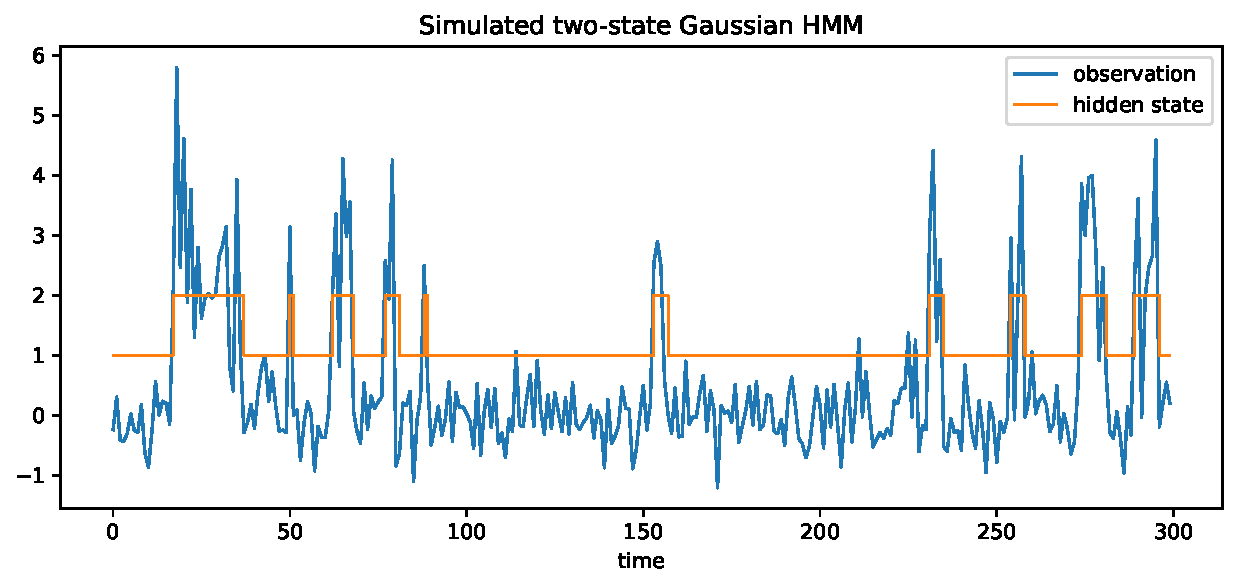
\includegraphics[keepaspectratio]{chapters/chapter-11-hidden-markov-regime-switching_files/figure-pdf/cell-2-output-1.pdf}}

A useful first diagnostic is to compare the sample behavior within the
true states.

\begin{Shaded}
\begin{Highlighting}[]
\ControlFlowTok{for}\NormalTok{ j }\KeywordTok{in} \BuiltInTok{range}\NormalTok{(}\DecValTok{2}\NormalTok{):}
\NormalTok{    values }\OperatorTok{=}\NormalTok{ y[states }\OperatorTok{==}\NormalTok{ j]}
    \BuiltInTok{print}\NormalTok{(}\SpecialStringTok{f"state }\SpecialCharTok{\{}\NormalTok{j }\OperatorTok{+} \DecValTok{1}\SpecialCharTok{\}}\SpecialStringTok{: count=}\SpecialCharTok{\{}\BuiltInTok{len}\NormalTok{(values)}\SpecialCharTok{:3d\}}\SpecialStringTok{, sample mean=}\SpecialCharTok{\{}\NormalTok{values}\SpecialCharTok{.}\NormalTok{mean()}\SpecialCharTok{: .3f\}}\SpecialStringTok{, sample sd=}\SpecialCharTok{\{}\NormalTok{values}\SpecialCharTok{.}\NormalTok{std(ddof}\OperatorTok{=}\DecValTok{1}\NormalTok{)}\SpecialCharTok{: .3f\}}\SpecialStringTok{"}\NormalTok{)}
\end{Highlighting}
\end{Shaded}

\begin{verbatim}
state 1: count=242, sample mean=-0.023, sample sd= 0.438
state 2: count= 58, sample mean= 2.536, sample sd= 1.305
\end{verbatim}

\section{11.15 Python example: scaled forward
filtering}\label{python-example-scaled-forward-filtering}

We now implement the forward algorithm. The function below returns the
filtered state probabilities and the log-likelihood.

\begin{Shaded}
\begin{Highlighting}[]
\KeywordTok{def}\NormalTok{ normal\_pdf(x, mean, sd):}
    \CommentTok{"""Gaussian density evaluated at x."""}
\NormalTok{    z }\OperatorTok{=}\NormalTok{ (x }\OperatorTok{{-}}\NormalTok{ mean) }\OperatorTok{/}\NormalTok{ sd}
    \ControlFlowTok{return}\NormalTok{ np.exp(}\OperatorTok{{-}}\FloatTok{0.5} \OperatorTok{*}\NormalTok{ z }\OperatorTok{*}\NormalTok{ z) }\OperatorTok{/}\NormalTok{ (np.sqrt(}\DecValTok{2} \OperatorTok{*}\NormalTok{ np.pi) }\OperatorTok{*}\NormalTok{ sd)}


\KeywordTok{def}\NormalTok{ forward\_scaled(y, pi, A, mu, sigma):}
    \CommentTok{"""Scaled forward algorithm for a Gaussian HMM."""}
\NormalTok{    y }\OperatorTok{=}\NormalTok{ np.asarray(y)}
\NormalTok{    K }\OperatorTok{=} \BuiltInTok{len}\NormalTok{(pi)}
\NormalTok{    T }\OperatorTok{=} \BuiltInTok{len}\NormalTok{(y)}

\NormalTok{    alpha }\OperatorTok{=}\NormalTok{ np.zeros((T, K))}
\NormalTok{    scales }\OperatorTok{=}\NormalTok{ np.zeros(T)}

\NormalTok{    emission }\OperatorTok{=}\NormalTok{ np.array([normal\_pdf(y[}\DecValTok{0}\NormalTok{], mu[j], sigma[j]) }\ControlFlowTok{for}\NormalTok{ j }\KeywordTok{in} \BuiltInTok{range}\NormalTok{(K)])}
\NormalTok{    unnormalized }\OperatorTok{=}\NormalTok{ pi }\OperatorTok{*}\NormalTok{ emission}
\NormalTok{    scales[}\DecValTok{0}\NormalTok{] }\OperatorTok{=}\NormalTok{ unnormalized.}\BuiltInTok{sum}\NormalTok{()}
\NormalTok{    alpha[}\DecValTok{0}\NormalTok{] }\OperatorTok{=}\NormalTok{ unnormalized }\OperatorTok{/}\NormalTok{ scales[}\DecValTok{0}\NormalTok{]}

    \ControlFlowTok{for}\NormalTok{ t }\KeywordTok{in} \BuiltInTok{range}\NormalTok{(}\DecValTok{1}\NormalTok{, T):}
\NormalTok{        prediction }\OperatorTok{=}\NormalTok{ alpha[t }\OperatorTok{{-}} \DecValTok{1}\NormalTok{] }\OperatorTok{@}\NormalTok{ A}
\NormalTok{        emission }\OperatorTok{=}\NormalTok{ np.array([normal\_pdf(y[t], mu[j], sigma[j]) }\ControlFlowTok{for}\NormalTok{ j }\KeywordTok{in} \BuiltInTok{range}\NormalTok{(K)])}
\NormalTok{        unnormalized }\OperatorTok{=}\NormalTok{ prediction }\OperatorTok{*}\NormalTok{ emission}
\NormalTok{        scales[t] }\OperatorTok{=}\NormalTok{ unnormalized.}\BuiltInTok{sum}\NormalTok{()}
\NormalTok{        alpha[t] }\OperatorTok{=}\NormalTok{ unnormalized }\OperatorTok{/}\NormalTok{ scales[t]}

\NormalTok{    loglik }\OperatorTok{=}\NormalTok{ np.log(scales).}\BuiltInTok{sum}\NormalTok{()}
    \ControlFlowTok{return}\NormalTok{ alpha, loglik}

\NormalTok{alpha, loglik }\OperatorTok{=}\NormalTok{ forward\_scaled(y, pi, A, mu, sigma)}
\BuiltInTok{print}\NormalTok{(}\SpecialStringTok{f"Log{-}likelihood under the true parameters: }\SpecialCharTok{\{}\NormalTok{loglik}\SpecialCharTok{:.2f\}}\SpecialStringTok{"}\NormalTok{)}
\BuiltInTok{print}\NormalTok{(}\StringTok{"Last filtered state probability:"}\NormalTok{, alpha[}\OperatorTok{{-}}\DecValTok{1}\NormalTok{])}
\end{Highlighting}
\end{Shaded}

\begin{verbatim}
Log-likelihood under the true parameters: -305.61
Last filtered state probability: [0.99479003 0.00520997]
\end{verbatim}

Plotting the filtered probability of state 2 shows how the model tracks
the hidden regime.

\begin{Shaded}
\begin{Highlighting}[]
\NormalTok{plt.figure(figsize}\OperatorTok{=}\NormalTok{(}\DecValTok{10}\NormalTok{, }\DecValTok{4}\NormalTok{))}
\NormalTok{plt.plot(alpha[:, }\DecValTok{1}\NormalTok{], label}\OperatorTok{=}\StringTok{"P(S\_t = 2 | y\_1:t)"}\NormalTok{)}
\NormalTok{plt.step(np.arange(T), states, where}\OperatorTok{=}\StringTok{"post"}\NormalTok{, alpha}\OperatorTok{=}\FloatTok{0.45}\NormalTok{, label}\OperatorTok{=}\StringTok{"true state 2 indicator"}\NormalTok{)}
\NormalTok{plt.ylim(}\OperatorTok{{-}}\FloatTok{0.05}\NormalTok{, }\FloatTok{1.05}\NormalTok{)}
\NormalTok{plt.title(}\StringTok{"Filtered probability of state 2"}\NormalTok{)}
\NormalTok{plt.xlabel(}\StringTok{"time"}\NormalTok{)}
\NormalTok{plt.legend()}
\NormalTok{plt.show()}
\end{Highlighting}
\end{Shaded}

\pandocbounded{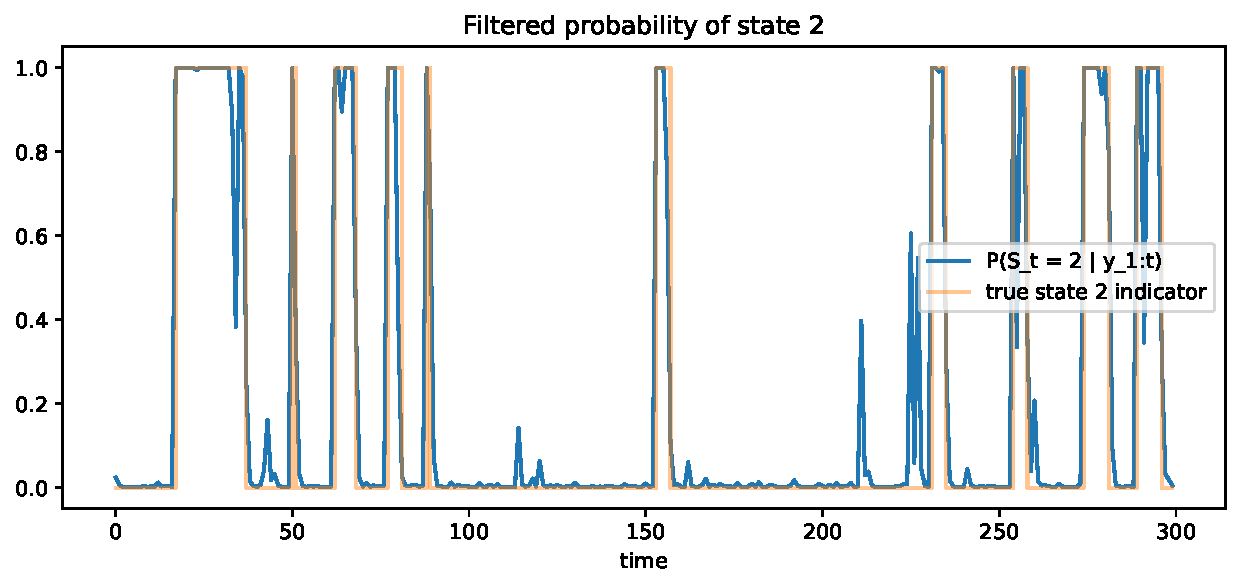
\includegraphics[keepaspectratio]{chapters/chapter-11-hidden-markov-regime-switching_files/figure-pdf/cell-5-output-1.pdf}}

\section{11.16 Python example: Viterbi
decoding}\label{python-example-viterbi-decoding}

The following function implements Viterbi decoding in log scale.

\begin{Shaded}
\begin{Highlighting}[]
\KeywordTok{def}\NormalTok{ viterbi\_gaussian(y, pi, A, mu, sigma):}
    \CommentTok{"""Most likely state path for a Gaussian HMM."""}
\NormalTok{    y }\OperatorTok{=}\NormalTok{ np.asarray(y)}
\NormalTok{    K }\OperatorTok{=} \BuiltInTok{len}\NormalTok{(pi)}
\NormalTok{    T }\OperatorTok{=} \BuiltInTok{len}\NormalTok{(y)}

\NormalTok{    log\_pi }\OperatorTok{=}\NormalTok{ np.log(pi)}
\NormalTok{    log\_A }\OperatorTok{=}\NormalTok{ np.log(A)}

\NormalTok{    log\_delta }\OperatorTok{=}\NormalTok{ np.zeros((T, K))}
\NormalTok{    psi }\OperatorTok{=}\NormalTok{ np.zeros((T, K), dtype}\OperatorTok{=}\BuiltInTok{int}\NormalTok{)}

\NormalTok{    log\_emission }\OperatorTok{=}\NormalTok{ np.array([}
\NormalTok{        np.log(normal\_pdf(y[}\DecValTok{0}\NormalTok{], mu[j], sigma[j])) }\ControlFlowTok{for}\NormalTok{ j }\KeywordTok{in} \BuiltInTok{range}\NormalTok{(K)}
\NormalTok{    ])}
\NormalTok{    log\_delta[}\DecValTok{0}\NormalTok{] }\OperatorTok{=}\NormalTok{ log\_pi }\OperatorTok{+}\NormalTok{ log\_emission}

    \ControlFlowTok{for}\NormalTok{ t }\KeywordTok{in} \BuiltInTok{range}\NormalTok{(}\DecValTok{1}\NormalTok{, T):}
        \ControlFlowTok{for}\NormalTok{ j }\KeywordTok{in} \BuiltInTok{range}\NormalTok{(K):}
\NormalTok{            candidates }\OperatorTok{=}\NormalTok{ log\_delta[t }\OperatorTok{{-}} \DecValTok{1}\NormalTok{] }\OperatorTok{+}\NormalTok{ log\_A[:, j]}
\NormalTok{            psi[t, j] }\OperatorTok{=}\NormalTok{ np.argmax(candidates)}
\NormalTok{            log\_delta[t, j] }\OperatorTok{=}\NormalTok{ candidates[psi[t, j]] }\OperatorTok{+}\NormalTok{ np.log(normal\_pdf(y[t], mu[j], sigma[j]))}

\NormalTok{    path }\OperatorTok{=}\NormalTok{ np.zeros(T, dtype}\OperatorTok{=}\BuiltInTok{int}\NormalTok{)}
\NormalTok{    path[}\OperatorTok{{-}}\DecValTok{1}\NormalTok{] }\OperatorTok{=}\NormalTok{ np.argmax(log\_delta[}\OperatorTok{{-}}\DecValTok{1}\NormalTok{])}
    \ControlFlowTok{for}\NormalTok{ t }\KeywordTok{in} \BuiltInTok{range}\NormalTok{(T }\OperatorTok{{-}} \DecValTok{2}\NormalTok{, }\OperatorTok{{-}}\DecValTok{1}\NormalTok{, }\OperatorTok{{-}}\DecValTok{1}\NormalTok{):}
\NormalTok{        path[t] }\OperatorTok{=}\NormalTok{ psi[t }\OperatorTok{+} \DecValTok{1}\NormalTok{, path[t }\OperatorTok{+} \DecValTok{1}\NormalTok{]]}

    \ControlFlowTok{return}\NormalTok{ path, log\_delta}

\NormalTok{path, log\_delta }\OperatorTok{=}\NormalTok{ viterbi\_gaussian(y, pi, A, mu, sigma)}
\NormalTok{accuracy }\OperatorTok{=}\NormalTok{ np.mean(path }\OperatorTok{==}\NormalTok{ states)}
\BuiltInTok{print}\NormalTok{(}\SpecialStringTok{f"Viterbi state decoding accuracy against simulated truth: }\SpecialCharTok{\{}\NormalTok{accuracy}\SpecialCharTok{:.3f\}}\SpecialStringTok{"}\NormalTok{)}
\end{Highlighting}
\end{Shaded}

\begin{verbatim}
Viterbi state decoding accuracy against simulated truth: 0.993
\end{verbatim}

\begin{Shaded}
\begin{Highlighting}[]
\NormalTok{plt.figure(figsize}\OperatorTok{=}\NormalTok{(}\DecValTok{10}\NormalTok{, }\DecValTok{4}\NormalTok{))}
\NormalTok{plt.step(np.arange(T), states }\OperatorTok{+} \DecValTok{1}\NormalTok{, where}\OperatorTok{=}\StringTok{"post"}\NormalTok{, label}\OperatorTok{=}\StringTok{"true hidden state"}\NormalTok{)}
\NormalTok{plt.step(np.arange(T), path }\OperatorTok{+} \DecValTok{1}\NormalTok{, where}\OperatorTok{=}\StringTok{"post"}\NormalTok{, linestyle}\OperatorTok{=}\StringTok{"{-}{-}"}\NormalTok{, label}\OperatorTok{=}\StringTok{"Viterbi decoded state"}\NormalTok{)}
\NormalTok{plt.yticks([}\DecValTok{1}\NormalTok{, }\DecValTok{2}\NormalTok{])}
\NormalTok{plt.title(}\StringTok{"True hidden path versus Viterbi decoded path"}\NormalTok{)}
\NormalTok{plt.xlabel(}\StringTok{"time"}\NormalTok{)}
\NormalTok{plt.legend()}
\NormalTok{plt.show()}
\end{Highlighting}
\end{Shaded}

\pandocbounded{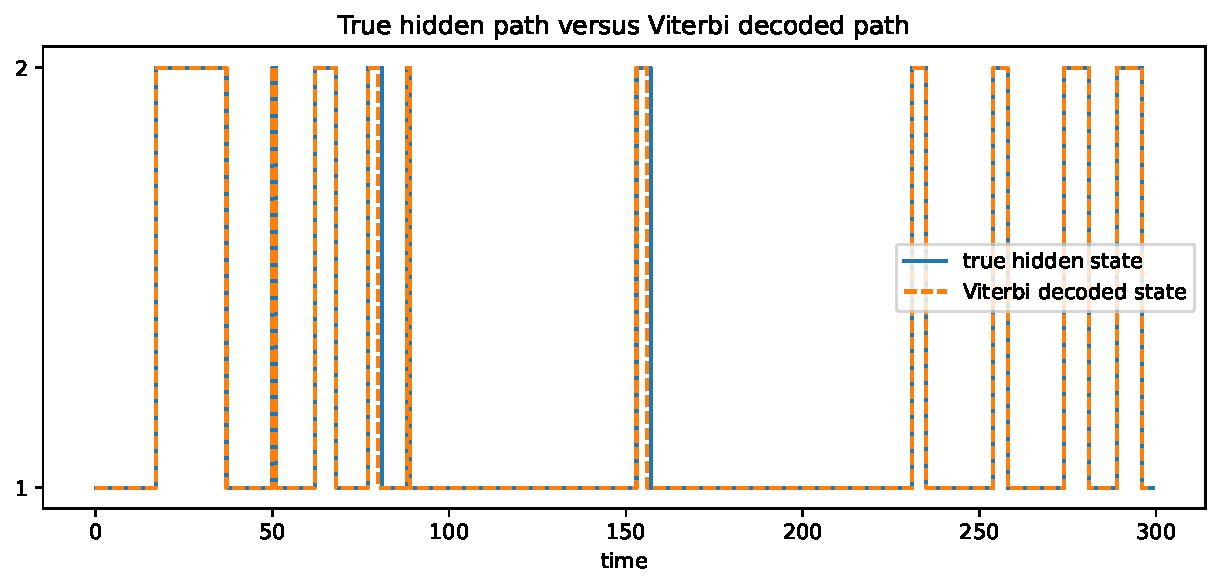
\includegraphics[keepaspectratio]{chapters/chapter-11-hidden-markov-regime-switching_files/figure-pdf/cell-7-output-1.pdf}}

\section{11.17 Python example: Baum--Welch for a Gaussian
HMM}\label{python-example-baumwelch-for-a-gaussian-hmm}

Here is a compact educational implementation of EM for a Gaussian HMM.
The goal is clarity, not production-level numerical robustness.

\begin{Shaded}
\begin{Highlighting}[]
\KeywordTok{def}\NormalTok{ forward\_backward\_scaled(y, pi, A, mu, sigma):}
    \CommentTok{"""Forward{-}backward algorithm for a Gaussian HMM."""}
\NormalTok{    y }\OperatorTok{=}\NormalTok{ np.asarray(y)}
\NormalTok{    K }\OperatorTok{=} \BuiltInTok{len}\NormalTok{(pi)}
\NormalTok{    T }\OperatorTok{=} \BuiltInTok{len}\NormalTok{(y)}

\NormalTok{    alpha, loglik }\OperatorTok{=}\NormalTok{ forward\_scaled(y, pi, A, mu, sigma)}

\NormalTok{    beta }\OperatorTok{=}\NormalTok{ np.ones((T, K))}
\NormalTok{    scales }\OperatorTok{=}\NormalTok{ np.zeros(T)}

    \CommentTok{\# Recompute scales from the forward pass.}
\NormalTok{    emission0 }\OperatorTok{=}\NormalTok{ np.array([normal\_pdf(y[}\DecValTok{0}\NormalTok{], mu[j], sigma[j]) }\ControlFlowTok{for}\NormalTok{ j }\KeywordTok{in} \BuiltInTok{range}\NormalTok{(K)])}
\NormalTok{    scales[}\DecValTok{0}\NormalTok{] }\OperatorTok{=}\NormalTok{ (pi }\OperatorTok{*}\NormalTok{ emission0).}\BuiltInTok{sum}\NormalTok{()}
    \ControlFlowTok{for}\NormalTok{ t }\KeywordTok{in} \BuiltInTok{range}\NormalTok{(}\DecValTok{1}\NormalTok{, T):}
\NormalTok{        pred }\OperatorTok{=}\NormalTok{ alpha[t }\OperatorTok{{-}} \DecValTok{1}\NormalTok{] }\OperatorTok{@}\NormalTok{ A}
\NormalTok{        emission }\OperatorTok{=}\NormalTok{ np.array([normal\_pdf(y[t], mu[j], sigma[j]) }\ControlFlowTok{for}\NormalTok{ j }\KeywordTok{in} \BuiltInTok{range}\NormalTok{(K)])}
\NormalTok{        scales[t] }\OperatorTok{=}\NormalTok{ (pred }\OperatorTok{*}\NormalTok{ emission).}\BuiltInTok{sum}\NormalTok{()}

    \ControlFlowTok{for}\NormalTok{ t }\KeywordTok{in} \BuiltInTok{range}\NormalTok{(T }\OperatorTok{{-}} \DecValTok{2}\NormalTok{, }\OperatorTok{{-}}\DecValTok{1}\NormalTok{, }\OperatorTok{{-}}\DecValTok{1}\NormalTok{):}
\NormalTok{        emission\_next }\OperatorTok{=}\NormalTok{ np.array([normal\_pdf(y[t }\OperatorTok{+} \DecValTok{1}\NormalTok{], mu[j], sigma[j]) }\ControlFlowTok{for}\NormalTok{ j }\KeywordTok{in} \BuiltInTok{range}\NormalTok{(K)])}
\NormalTok{        beta[t] }\OperatorTok{=}\NormalTok{ A }\OperatorTok{@}\NormalTok{ (emission\_next }\OperatorTok{*}\NormalTok{ beta[t }\OperatorTok{+} \DecValTok{1}\NormalTok{])}
\NormalTok{        beta[t] }\OperatorTok{=}\NormalTok{ beta[t] }\OperatorTok{/}\NormalTok{ scales[t }\OperatorTok{+} \DecValTok{1}\NormalTok{]}

\NormalTok{    gamma }\OperatorTok{=}\NormalTok{ alpha }\OperatorTok{*}\NormalTok{ beta}
\NormalTok{    gamma }\OperatorTok{=}\NormalTok{ gamma }\OperatorTok{/}\NormalTok{ gamma.}\BuiltInTok{sum}\NormalTok{(axis}\OperatorTok{=}\DecValTok{1}\NormalTok{, keepdims}\OperatorTok{=}\VariableTok{True}\NormalTok{)}

\NormalTok{    xi }\OperatorTok{=}\NormalTok{ np.zeros((T }\OperatorTok{{-}} \DecValTok{1}\NormalTok{, K, K))}
    \ControlFlowTok{for}\NormalTok{ t }\KeywordTok{in} \BuiltInTok{range}\NormalTok{(T }\OperatorTok{{-}} \DecValTok{1}\NormalTok{):}
\NormalTok{        emission\_next }\OperatorTok{=}\NormalTok{ np.array([normal\_pdf(y[t }\OperatorTok{+} \DecValTok{1}\NormalTok{], mu[j], sigma[j]) }\ControlFlowTok{for}\NormalTok{ j }\KeywordTok{in} \BuiltInTok{range}\NormalTok{(K)])}
\NormalTok{        numerator }\OperatorTok{=}\NormalTok{ alpha[t, :, }\VariableTok{None}\NormalTok{] }\OperatorTok{*}\NormalTok{ A }\OperatorTok{*}\NormalTok{ emission\_next[}\VariableTok{None}\NormalTok{, :] }\OperatorTok{*}\NormalTok{ beta[t }\OperatorTok{+} \DecValTok{1}\NormalTok{, }\VariableTok{None}\NormalTok{, :]}
\NormalTok{        xi[t] }\OperatorTok{=}\NormalTok{ numerator }\OperatorTok{/}\NormalTok{ numerator.}\BuiltInTok{sum}\NormalTok{()}

    \ControlFlowTok{return}\NormalTok{ gamma, xi, loglik}


\KeywordTok{def}\NormalTok{ baum\_welch\_gaussian(y, K}\OperatorTok{=}\DecValTok{2}\NormalTok{, n\_iter}\OperatorTok{=}\DecValTok{30}\NormalTok{, seed}\OperatorTok{=}\DecValTok{1}\NormalTok{):}
    \CommentTok{"""Simple EM algorithm for a Gaussian HMM."""}
\NormalTok{    rng }\OperatorTok{=}\NormalTok{ np.random.default\_rng(seed)}
\NormalTok{    y }\OperatorTok{=}\NormalTok{ np.asarray(y)}
\NormalTok{    T }\OperatorTok{=} \BuiltInTok{len}\NormalTok{(y)}

\NormalTok{    pi\_est }\OperatorTok{=}\NormalTok{ np.ones(K) }\OperatorTok{/}\NormalTok{ K}
\NormalTok{    A\_est }\OperatorTok{=}\NormalTok{ np.full((K, K), }\DecValTok{1} \OperatorTok{/}\NormalTok{ K)}
\NormalTok{    A\_est }\OperatorTok{=} \FloatTok{0.85} \OperatorTok{*}\NormalTok{ np.eye(K) }\OperatorTok{+} \FloatTok{0.15} \OperatorTok{*}\NormalTok{ A\_est}
\NormalTok{    mu\_est }\OperatorTok{=}\NormalTok{ np.quantile(y, np.linspace(}\FloatTok{0.25}\NormalTok{, }\FloatTok{0.75}\NormalTok{, K))}
\NormalTok{    sigma\_est }\OperatorTok{=}\NormalTok{ np.full(K, np.std(y))}

\NormalTok{    history }\OperatorTok{=}\NormalTok{ []}
    \ControlFlowTok{for}\NormalTok{ \_ }\KeywordTok{in} \BuiltInTok{range}\NormalTok{(n\_iter):}
\NormalTok{        gamma, xi, loglik }\OperatorTok{=}\NormalTok{ forward\_backward\_scaled(y, pi\_est, A\_est, mu\_est, sigma\_est)}
\NormalTok{        history.append(loglik)}

\NormalTok{        pi\_est }\OperatorTok{=}\NormalTok{ gamma[}\DecValTok{0}\NormalTok{]}
\NormalTok{        A\_est }\OperatorTok{=}\NormalTok{ xi.}\BuiltInTok{sum}\NormalTok{(axis}\OperatorTok{=}\DecValTok{0}\NormalTok{) }\OperatorTok{/}\NormalTok{ gamma[:}\OperatorTok{{-}}\DecValTok{1}\NormalTok{].}\BuiltInTok{sum}\NormalTok{(axis}\OperatorTok{=}\DecValTok{0}\NormalTok{, keepdims}\OperatorTok{=}\VariableTok{True}\NormalTok{).T}

\NormalTok{        weights }\OperatorTok{=}\NormalTok{ gamma.}\BuiltInTok{sum}\NormalTok{(axis}\OperatorTok{=}\DecValTok{0}\NormalTok{)}
\NormalTok{        mu\_est }\OperatorTok{=}\NormalTok{ (gamma }\OperatorTok{*}\NormalTok{ y[:, }\VariableTok{None}\NormalTok{]).}\BuiltInTok{sum}\NormalTok{(axis}\OperatorTok{=}\DecValTok{0}\NormalTok{) }\OperatorTok{/}\NormalTok{ weights}
\NormalTok{        sigma\_est }\OperatorTok{=}\NormalTok{ np.sqrt((gamma }\OperatorTok{*}\NormalTok{ (y[:, }\VariableTok{None}\NormalTok{] }\OperatorTok{{-}}\NormalTok{ mu\_est[}\VariableTok{None}\NormalTok{, :])}\OperatorTok{**}\DecValTok{2}\NormalTok{).}\BuiltInTok{sum}\NormalTok{(axis}\OperatorTok{=}\DecValTok{0}\NormalTok{) }\OperatorTok{/}\NormalTok{ weights)}
\NormalTok{        sigma\_est }\OperatorTok{=}\NormalTok{ np.maximum(sigma\_est, }\FloatTok{1e{-}4}\NormalTok{)}

    \ControlFlowTok{return}\NormalTok{ pi\_est, A\_est, mu\_est, sigma\_est, np.array(history)}

\NormalTok{pi\_hat, A\_hat, mu\_hat, sigma\_hat, history }\OperatorTok{=}\NormalTok{ baum\_welch\_gaussian(y, K}\OperatorTok{=}\DecValTok{2}\NormalTok{, n\_iter}\OperatorTok{=}\DecValTok{40}\NormalTok{, seed}\OperatorTok{=}\DecValTok{5}\NormalTok{)}
\BuiltInTok{print}\NormalTok{(}\StringTok{"Estimated pi:"}\NormalTok{, np.}\BuiltInTok{round}\NormalTok{(pi\_hat, }\DecValTok{3}\NormalTok{))}
\BuiltInTok{print}\NormalTok{(}\StringTok{"Estimated A:}\CharTok{\textbackslash{}n}\StringTok{"}\NormalTok{, np.}\BuiltInTok{round}\NormalTok{(A\_hat, }\DecValTok{3}\NormalTok{))}
\BuiltInTok{print}\NormalTok{(}\StringTok{"Estimated means:"}\NormalTok{, np.}\BuiltInTok{round}\NormalTok{(mu\_hat, }\DecValTok{3}\NormalTok{))}
\BuiltInTok{print}\NormalTok{(}\StringTok{"Estimated standard deviations:"}\NormalTok{, np.}\BuiltInTok{round}\NormalTok{(sigma\_hat, }\DecValTok{3}\NormalTok{))}
\end{Highlighting}
\end{Shaded}

\begin{verbatim}
Estimated pi: [1. 0.]
Estimated A:
 [[0.95 0.05]
 [0.21 0.79]]
Estimated means: [-0.029  2.591]
Estimated standard deviations: [0.434 1.221]
\end{verbatim}

\begin{Shaded}
\begin{Highlighting}[]
\NormalTok{plt.figure(figsize}\OperatorTok{=}\NormalTok{(}\DecValTok{8}\NormalTok{, }\DecValTok{4}\NormalTok{))}
\NormalTok{plt.plot(history, marker}\OperatorTok{=}\StringTok{"o"}\NormalTok{)}
\NormalTok{plt.title(}\StringTok{"Baum{-}{-}Welch log{-}likelihood trace"}\NormalTok{)}
\NormalTok{plt.xlabel(}\StringTok{"EM iteration"}\NormalTok{)}
\NormalTok{plt.ylabel(}\StringTok{"log{-}likelihood"}\NormalTok{)}
\NormalTok{plt.show()}
\end{Highlighting}
\end{Shaded}

\pandocbounded{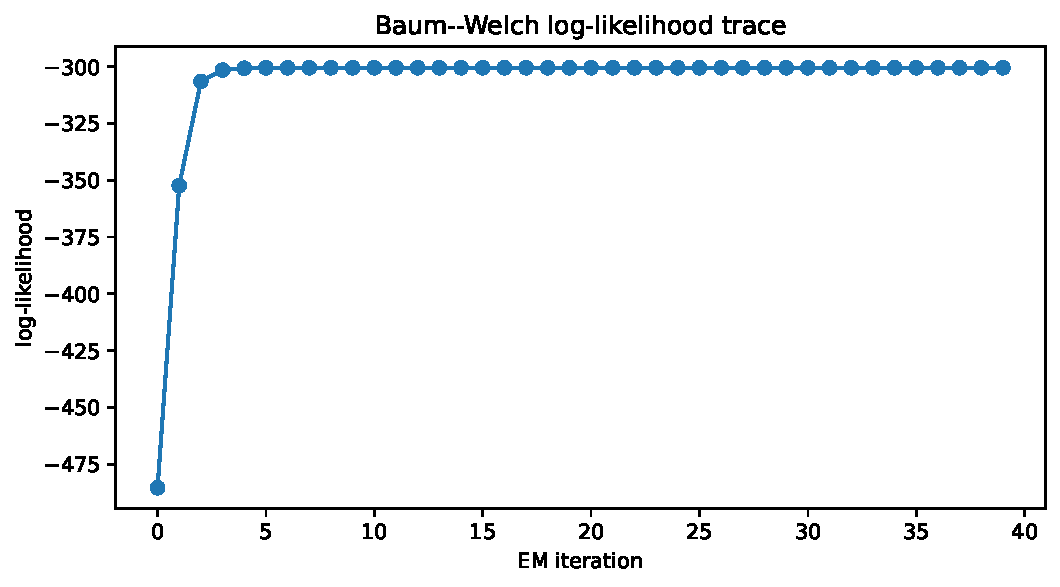
\includegraphics[keepaspectratio]{chapters/chapter-11-hidden-markov-regime-switching_files/figure-pdf/cell-9-output-1.pdf}}

The likelihood should generally increase. Small numerical decreases can
occur if the implementation is unstable, but a clean EM implementation
should be monotone up to floating-point error.

\section{11.18 Model selection and
diagnostics}\label{model-selection-and-diagnostics}

Choosing the number of hidden states \(K\) is a modeling decision. More
states increase flexibility but can make interpretation unstable.

Common strategies include:

\begin{enumerate}
\def\labelenumi{\arabic{enumi}.}
\tightlist
\item
  \textbf{Domain interpretation:} choose states that correspond to
  meaningful regimes.
\item
  \textbf{Information criteria:} compare AIC or BIC across values of
  \(K\).
\item
  \textbf{Out-of-sample performance:} compare forecast or classification
  performance.
\item
  \textbf{State persistence:} check whether transition probabilities are
  interpretable.
\item
  \textbf{Posterior uncertainty:} inspect whether state probabilities
  are decisive or ambiguous.
\item
  \textbf{Residual checks:} after conditioning on decoded or smoothed
  states, examine residual behavior.
\end{enumerate}

For a fitted Gaussian HMM, state-specific standardized residuals are

\[
r_t^{(j)}=\frac{y_t-\widehat{\mu}_j}{\widehat{\sigma}_j}.
\]

A soft residual can use smoothed probabilities:

\[
\widehat{\mu}_t=\sum_{j=1}^K \gamma_t(j)\widehat{\mu}_j,
\]

\[
\widehat{\sigma}_t^2
=\sum_{j=1}^K \gamma_t(j)\left[\widehat{\sigma}_j^2+(\widehat{\mu}_j-\widehat{\mu}_t)^2\right],
\]

and

\[
r_t=\frac{y_t-\widehat{\mu}_t}{\widehat{\sigma}_t}.
\]

Then we can inspect time plots, ACF plots, and distributional
diagnostics of \(r_t\).

\begin{tcolorbox}[enhanced jigsaw, arc=.35mm, bottomrule=.15mm, bottomtitle=1mm, breakable, colback=white, colbacktitle=quarto-callout-warning-color!10!white, colframe=quarto-callout-warning-color-frame, coltitle=black, left=2mm, leftrule=.75mm, opacityback=0, opacitybacktitle=0.6, rightrule=.15mm, title=\textcolor{quarto-callout-warning-color}{\faExclamationTriangle}\hspace{0.5em}{Label switching}, titlerule=0mm, toprule=.15mm, toptitle=1mm]

The labels of hidden states are arbitrary. If state 1 and state 2 are
swapped, the likelihood is unchanged. Interpret states by their
estimated means, variances, persistence, or application meaning, not by
their numeric labels.

\end{tcolorbox}

\section{11.19 HMMs and modern AI sequence
models}\label{hmms-and-modern-ai-sequence-models}

HMMs are classical probabilistic sequence models. They remain important
because they expose ideas that also appear in modern AI systems.

{\def\LTcaptype{none} % do not increment counter
\begin{longtable}[]{@{}ll@{}}
\toprule\noalign{}
HMM idea & Modern sequence-learning analogue \\
\midrule\noalign{}
\endhead
\bottomrule\noalign{}
\endlastfoot
Hidden state \(S_t\) & latent representation or memory state \\
Transition matrix \(\mathbf{A}\) & learned state update rule \\
Emission distribution \(b_j(y)\) & decoder or output distribution \\
Forward filtering & sequential inference \\
Viterbi decoding & most likely structured prediction \\
Baum--Welch & latent-variable training \\
Regime probabilities & interpretable uncertainty over modes \\
\end{longtable}
}

RNNs, LSTMs, GRUs, and transformers replace discrete hand-specified
state dynamics with flexible learned functions. However, HMMs remain
useful when interpretability, small data, uncertainty, or regime
structure matters.

\section{11.20 AI-assisted modeling
component}\label{ai-assisted-modeling-component-1}

AI tools can help with HMMs, but they often make subtle mistakes with
scaling, indexing, and interpretation. Use AI as a critic and
collaborator, not as the source of truth.

\begin{tcolorbox}[enhanced jigsaw, arc=.35mm, bottomrule=.15mm, bottomtitle=1mm, breakable, colback=white, colbacktitle=quarto-callout-tip-color!10!white, colframe=quarto-callout-tip-color-frame, coltitle=black, left=2mm, leftrule=.75mm, opacityback=0, opacitybacktitle=0.6, rightrule=.15mm, title=\textcolor{quarto-callout-tip-color}{\faLightbulb}\hspace{0.5em}{Prompt: code audit}, titlerule=0mm, toprule=.15mm, toptitle=1mm]

I implemented the scaled forward algorithm for a Gaussian HMM. Please
check the dimensions, normalization, likelihood calculation, and
possible underflow problems. Do not rewrite the code first. Identify
mathematical or indexing mistakes and explain how to test each one.

\end{tcolorbox}

\begin{tcolorbox}[enhanced jigsaw, arc=.35mm, bottomrule=.15mm, bottomtitle=1mm, breakable, colback=white, colbacktitle=quarto-callout-tip-color!10!white, colframe=quarto-callout-tip-color-frame, coltitle=black, left=2mm, leftrule=.75mm, opacityback=0, opacitybacktitle=0.6, rightrule=.15mm, title=\textcolor{quarto-callout-tip-color}{\faLightbulb}\hspace{0.5em}{Prompt: model critique}, titlerule=0mm, toprule=.15mm, toptitle=1mm]

I fitted a two-state Gaussian HMM to a financial return series. State 1
has low variance and state 2 has high variance. The transition
probabilities are 0.97 and 0.91 on the diagonal. What diagnostics should
I check before claiming these are calm and crisis regimes? Include tests
for residual autocorrelation, outliers, label switching, and stability
across initializations.

\end{tcolorbox}

\begin{tcolorbox}[enhanced jigsaw, arc=.35mm, bottomrule=.15mm, bottomtitle=1mm, breakable, colback=white, colbacktitle=quarto-callout-tip-color!10!white, colframe=quarto-callout-tip-color-frame, coltitle=black, left=2mm, leftrule=.75mm, opacityback=0, opacitybacktitle=0.6, rightrule=.15mm, title=\textcolor{quarto-callout-tip-color}{\faLightbulb}\hspace{0.5em}{Prompt: interpretation guardrail}, titlerule=0mm, toprule=.15mm, toptitle=1mm]

Here is a plot of smoothed state probabilities from an HMM. Help me
write a cautious interpretation. Avoid saying the hidden state is
directly observed. Use language such as ``the model assigns high
posterior probability to\ldots'' and distinguish model-based regimes
from true causal regimes.

\end{tcolorbox}

\subsection{Human verification
checklist}\label{human-verification-checklist}

Whenever an AI tool helps with HMM code or interpretation, manually
check:

\begin{enumerate}
\def\labelenumi{\arabic{enumi}.}
\tightlist
\item
  rows of \(\mathbf{A}\) sum to one;
\item
  all probabilities are nonnegative;
\item
  forward probabilities are normalized at each time;
\item
  log-likelihood is computed from scaling constants or log-sum-exp;
\item
  Viterbi output uses backpointers correctly;
\item
  EM likelihood increases across iterations;
\item
  fitted states are stable across random initializations;
\item
  interpretation does not confuse latent states with observed ground
  truth.
\end{enumerate}

\section{11.21 Common mistakes}\label{common-mistakes-10}

\begin{tcolorbox}[enhanced jigsaw, arc=.35mm, bottomrule=.15mm, bottomtitle=1mm, breakable, colback=white, colbacktitle=quarto-callout-warning-color!10!white, colframe=quarto-callout-warning-color-frame, coltitle=black, left=2mm, leftrule=.75mm, opacityback=0, opacitybacktitle=0.6, rightrule=.15mm, title=\textcolor{quarto-callout-warning-color}{\faExclamationTriangle}\hspace{0.5em}{Mistake 1: treating hidden states as observed labels}, titlerule=0mm, toprule=.15mm, toptitle=1mm]

The hidden states are model-based latent variables. Unless the data
include true labels, decoded states are estimates, not facts.

\end{tcolorbox}

\begin{tcolorbox}[enhanced jigsaw, arc=.35mm, bottomrule=.15mm, bottomtitle=1mm, breakable, colback=white, colbacktitle=quarto-callout-warning-color!10!white, colframe=quarto-callout-warning-color-frame, coltitle=black, left=2mm, leftrule=.75mm, opacityback=0, opacitybacktitle=0.6, rightrule=.15mm, title=\textcolor{quarto-callout-warning-color}{\faExclamationTriangle}\hspace{0.5em}{Mistake 2: ignoring numerical scaling}, titlerule=0mm, toprule=.15mm, toptitle=1mm]

Unscaled forward probabilities usually underflow for long sequences. Use
scaled probabilities or log-sum-exp.

\end{tcolorbox}

\begin{tcolorbox}[enhanced jigsaw, arc=.35mm, bottomrule=.15mm, bottomtitle=1mm, breakable, colback=white, colbacktitle=quarto-callout-warning-color!10!white, colframe=quarto-callout-warning-color-frame, coltitle=black, left=2mm, leftrule=.75mm, opacityback=0, opacitybacktitle=0.6, rightrule=.15mm, title=\textcolor{quarto-callout-warning-color}{\faExclamationTriangle}\hspace{0.5em}{Mistake 3: comparing state labels across fits}, titlerule=0mm, toprule=.15mm, toptitle=1mm]

State 1 in one fit may correspond to state 2 in another. Compare states
by their parameters, not their labels.

\end{tcolorbox}

\begin{tcolorbox}[enhanced jigsaw, arc=.35mm, bottomrule=.15mm, bottomtitle=1mm, breakable, colback=white, colbacktitle=quarto-callout-warning-color!10!white, colframe=quarto-callout-warning-color-frame, coltitle=black, left=2mm, leftrule=.75mm, opacityback=0, opacitybacktitle=0.6, rightrule=.15mm, title=\textcolor{quarto-callout-warning-color}{\faExclamationTriangle}\hspace{0.5em}{Mistake 4: using too many states}, titlerule=0mm, toprule=.15mm, toptitle=1mm]

A model with many states may fit the training sequence better but
produce unstable, uninterpretable, or non-reproducible regimes.

\end{tcolorbox}

\begin{tcolorbox}[enhanced jigsaw, arc=.35mm, bottomrule=.15mm, bottomtitle=1mm, breakable, colback=white, colbacktitle=quarto-callout-warning-color!10!white, colframe=quarto-callout-warning-color-frame, coltitle=black, left=2mm, leftrule=.75mm, opacityback=0, opacitybacktitle=0.6, rightrule=.15mm, title=\textcolor{quarto-callout-warning-color}{\faExclamationTriangle}\hspace{0.5em}{Mistake 5: forgetting time-series dependence inside regimes}, titlerule=0mm, toprule=.15mm, toptitle=1mm]

A Gaussian HMM may not remove autocorrelation. If residuals remain
autocorrelated within states, consider a Markov-switching AR model.

\end{tcolorbox}

\section{11.22 Exercises}\label{exercises-10}

\subsection{Conceptual exercises}\label{conceptual-exercises-8}

\begin{enumerate}
\def\labelenumi{\arabic{enumi}.}
\tightlist
\item
  Explain the difference between a Markov chain and a hidden Markov
  model.
\item
  In a two-state HMM with \(a_{11}=0.98\) and \(a_{22}=0.80\), compute
  the expected duration of each state.
\item
  Explain why direct likelihood computation requires summing over
  \(K^T\) paths.
\item
  Explain the difference between filtering probability, smoothing
  probability, and Viterbi decoding.
\item
  Give an example where the Viterbi path and the pointwise most likely
  states may differ.
\end{enumerate}

\subsection{Mathematical exercises}\label{mathematical-exercises-7}

\begin{enumerate}
\def\labelenumi{\arabic{enumi}.}
\tightlist
\item
  Derive the forward recursion from the joint probability formula.
\item
  Derive the backward recursion.
\item
  Show that \(\sum_j \gamma_t(j)=1\).
\item
  Derive the Baum--Welch update for \(a_{ij}\) using expected transition
  counts.
\item
  Derive the weighted Gaussian updates for \(\mu_j\) and \(\sigma_j^2\).
\item
  For a Gaussian HMM, derive the one-step forecast mean and variance
  using the law of total expectation and law of total variance.
\end{enumerate}

\subsection{Computational exercises}\label{computational-exercises-5}

\begin{enumerate}
\def\labelenumi{\arabic{enumi}.}
\tightlist
\item
  Simulate a three-state Gaussian HMM and plot the hidden states and
  observations.
\item
  Implement the scaled forward algorithm and verify that filtered
  probabilities sum to one.
\item
  Implement Viterbi decoding and compare the decoded path to the true
  simulated path.
\item
  Fit a two-state Gaussian HMM using the Baum--Welch code and test
  several random initializations.
\item
  Modify the emission distribution to use state-dependent Poisson
  distributions for count data.
\item
  Implement a Markov-switching AR(1) filter by replacing \(b_j(y_t)\)
  with \(b_j(y_t\mid y_{t-1})\).
\end{enumerate}

\section{11.23 Mini project: regime detection in a real
sequence}\label{mini-project-regime-detection-in-a-real-sequence}

Choose one real sequence dataset. Possible choices include:

\begin{itemize}
\tightlist
\item
  daily financial returns;
\item
  hourly electricity demand changes;
\item
  machine vibration or sensor data;
\item
  weather anomalies;
\item
  web traffic or user activity counts;
\item
  biological signal measurements.
\end{itemize}

Your report should include:

\begin{enumerate}
\def\labelenumi{\arabic{enumi}.}
\tightlist
\item
  exploratory plots and summary statistics;
\item
  justification for the number of states \(K\);
\item
  fitted transition matrix and emission parameters;
\item
  filtered and smoothed state probability plots;
\item
  Viterbi decoded path;
\item
  residual diagnostics;
\item
  out-of-sample forecasting or anomaly-detection evaluation;
\item
  an AI-assisted critique section describing how you used AI and how you
  verified its suggestions.
\end{enumerate}

\section{11.24 Chapter checklist}\label{chapter-checklist-8}

By the end of this chapter, you should be able to:

\begin{itemize}
\tightlist
\item[$\square$]
  define an HMM using initial, transition, and emission probabilities;
\item[$\square$]
  write the joint probability of hidden states and observations;
\item[$\square$]
  compute likelihood with the forward algorithm;
\item[$\square$]
  explain why scaling is needed;
\item[$\square$]
  compute smoothed state probabilities using forward--backward
  recursions;
\item[$\square$]
  decode a hidden path using Viterbi;
\item[$\square$]
  explain Baum--Welch as EM;
\item[$\square$]
  fit and interpret a Gaussian HMM;
\item[$\square$]
  explain how regime-switching AR models extend Gaussian HMMs;
\item[$\square$]
  forecast from a fitted HMM using state probability propagation;
\item[$\square$]
  evaluate diagnostics and avoid overinterpreting hidden states;
\item[$\square$]
  use AI tools carefully for debugging, critique, and communication.
\end{itemize}

\section{11.25 Looking ahead}\label{looking-ahead}

State-space models and HMMs provide two classical hidden-state
frameworks:

\[
\text{continuous hidden state} \quad \leftrightarrow \quad \text{Kalman filter},
\]

\[
\text{discrete hidden state} \quad \leftrightarrow \quad \text{HMM}.
\]

The next part of the book moves from hidden-state time-domain models to
frequency-domain methods. Instead of asking which hidden regime
generated the observation, we ask which oscillatory components explain
the variation in the sequence.

\part{Part IV. Frequency-Domain and Multiresolution Methods}

\chapter{Spectral Analysis and the Frequency
Domain}\label{spectral-analysis-and-the-frequency-domain}

\textbf{Part IV. Frequency-Domain and Multiresolution Methods}\\
\textbf{Chapter goal:} learn how to describe second-order dependence by
frequency rather than by lag. We develop periodic signals, aliasing,
random sinusoidal models, spectral distributions, spectral densities,
spectra of ARMA models, and AI-assisted interpretation of
frequency-domain evidence.

\section{Learning objectives}\label{learning-objectives-11}

After studying this chapter, you should be able to:

\begin{enumerate}
\def\labelenumi{\arabic{enumi}.}
\tightlist
\item
  explain the difference between time-domain and frequency-domain views
  of a time series;
\item
  interpret frequency, period, amplitude, and phase in a discrete-time
  sequence;
\item
  explain aliasing and the Nyquist frequency;
\item
  show that random sinusoidal models can be stationary;
\item
  define the spectral distribution and spectral density of a stationary
  process;
\item
  use the identity between autocovariance and spectral density;
\item
  interpret \(f(\omega)\) as variance per frequency;
\item
  derive spectra of white noise, AR(1), MA(1), and causal ARMA models;
\item
  connect spectral peaks with oscillatory behavior in the time domain;
\item
  use AI tools to formulate hypotheses about periodicity while verifying
  them with mathematics and code.
\end{enumerate}

\section{12.1 Why frequency-domain
thinking?}\label{why-frequency-domain-thinking}

The earlier chapters used the \textbf{time domain}. In the time-domain
approach, the central question is:

\begin{quote}
How does the present depend on the past?
\end{quote}

For example, an AR(1) model says

\[
X_t=\phi X_{t-1}+W_t.
\]

This is a rule for moving forward in time. The model describes how the
current observation is generated from past observations and new noise.

The \textbf{frequency-domain} approach asks a different question:

\begin{quote}
Which oscillations explain the variation in the series?
\end{quote}

Many time series contain repeated patterns: daily electricity demand,
annual climate cycles, weekly web traffic, business cycles, speech
waveforms, sensor vibrations, and seasonal sales. Instead of regressing
\(X_t\) on \(X_{t-1},X_{t-2},\ldots\), spectral analysis studies how
much variance is associated with low, medium, or high frequencies.

A rough translation is:

{\def\LTcaptype{none} % do not increment counter
\begin{longtable}[]{@{}ll@{}}
\toprule\noalign{}
Time-domain language & Frequency-domain language \\
\midrule\noalign{}
\endhead
\bottomrule\noalign{}
\endlastfoot
dependence across lags & variance across frequencies \\
autocovariance \(\gamma(h)\) & spectral density \(f(\omega)\) \\
AR/MA recursions & filters and frequency response \\
slow ACF decay & strong low-frequency power \\
alternating signs & strong high-frequency power \\
\end{longtable}
}

\begin{tcolorbox}[enhanced jigsaw, arc=.35mm, bottomrule=.15mm, bottomtitle=1mm, breakable, colback=white, colbacktitle=quarto-callout-note-color!10!white, colframe=quarto-callout-note-color-frame, coltitle=black, left=2mm, leftrule=.75mm, opacityback=0, opacitybacktitle=0.6, rightrule=.15mm, title=\textcolor{quarto-callout-note-color}{\faInfo}\hspace{0.5em}{Same information, different coordinates}, titlerule=0mm, toprule=.15mm, toptitle=1mm]

For a stationary process, the autocovariance function and the spectral
density are Fourier-transform pairs. They are two coordinate systems for
the same second-order information.

\end{tcolorbox}

\section{12.2 Period, frequency, amplitude, and
phase}\label{period-frequency-amplitude-and-phase}

A basic periodic component can be written as

\[
\mu_t=A\cos(2\pi \omega t+\varphi),
\]

where:

\begin{itemize}
\tightlist
\item
  \(A\) is the amplitude;
\item
  \(\omega\) is the frequency, measured in cycles per time step;
\item
  \(1/\omega\) is the period, measured in time steps per cycle;
\item
  \(\varphi\) is the phase shift.
\end{itemize}

If \(\omega=1/12\), then the period is \(12\). For monthly data, this
corresponds to one cycle per year. If \(\omega=1/7\), then the period is
\(7\). For daily data, this corresponds to weekly seasonality.

The phase parameter can be removed from the nonlinear expression using a
trigonometric identity:

\[
A\cos(2\pi\omega t+\varphi)
=A\cos(\varphi)\cos(2\pi\omega t)-A\sin(\varphi)\sin(2\pi\omega t).
\]

Thus we may write

\[
A\cos(2\pi\omega t+\varphi)
=\beta_c\cos(2\pi\omega t)+\beta_s\sin(2\pi\omega t),
\]

where

\[
\beta_c=A\cos(\varphi),
\qquad
\beta_s=-A\sin(\varphi).
\]

This is important computationally: once the frequency \(\omega\) is
fixed, fitting a sinusoidal component becomes an ordinary linear
regression problem.

\subsection{Example: regression on
sinusoids}\label{example-regression-on-sinusoids}

Suppose

\[
X_t=\beta_0+\beta_c\cos(2\pi\omega t)+\beta_s\sin(2\pi\omega t)+E_t.
\]

Let

\[
\mathbf{z}_t=\begin{bmatrix}1\\ \cos(2\pi\omega t)\\ \sin(2\pi\omega t)\end{bmatrix},
\qquad
\boldsymbol{\beta}=\begin{bmatrix}\beta_0\\ \beta_c\\ \beta_s\end{bmatrix}.
\]

Then

\[
X_t=\boldsymbol{\beta}^{\top}\mathbf{z}_t+E_t.
\]

For a fixed \(\omega\), ordinary least squares estimates
\(\boldsymbol{\beta}\). The fitted amplitude and phase can be recovered
from

\[
\widehat{A}=\sqrt{\widehat{\beta}_c^2+\widehat{\beta}_s^2}.
\]

The phase is recovered up to the sign convention used for the sine term.

\begin{Shaded}
\begin{Highlighting}[]
\ImportTok{import}\NormalTok{ numpy }\ImportTok{as}\NormalTok{ np}
\ImportTok{import}\NormalTok{ matplotlib.pyplot }\ImportTok{as}\NormalTok{ plt}

\NormalTok{rng }\OperatorTok{=}\NormalTok{ np.random.default\_rng(}\DecValTok{7339}\NormalTok{)}
\NormalTok{n }\OperatorTok{=} \DecValTok{180}
\NormalTok{t }\OperatorTok{=}\NormalTok{ np.arange(n)}
\NormalTok{omega }\OperatorTok{=} \DecValTok{1} \OperatorTok{/} \DecValTok{30}

\NormalTok{x }\OperatorTok{=} \FloatTok{2.0} \OperatorTok{+} \FloatTok{1.5} \OperatorTok{*}\NormalTok{ np.cos(}\DecValTok{2} \OperatorTok{*}\NormalTok{ np.pi }\OperatorTok{*}\NormalTok{ omega }\OperatorTok{*}\NormalTok{ t }\OperatorTok{+} \FloatTok{0.8}\NormalTok{) }\OperatorTok{+} \FloatTok{0.5} \OperatorTok{*}\NormalTok{ rng.normal(size}\OperatorTok{=}\NormalTok{n)}

\NormalTok{Z }\OperatorTok{=}\NormalTok{ np.column\_stack([}
\NormalTok{    np.ones(n),}
\NormalTok{    np.cos(}\DecValTok{2} \OperatorTok{*}\NormalTok{ np.pi }\OperatorTok{*}\NormalTok{ omega }\OperatorTok{*}\NormalTok{ t),}
\NormalTok{    np.sin(}\DecValTok{2} \OperatorTok{*}\NormalTok{ np.pi }\OperatorTok{*}\NormalTok{ omega }\OperatorTok{*}\NormalTok{ t),}
\NormalTok{])}
\NormalTok{beta\_hat }\OperatorTok{=}\NormalTok{ np.linalg.lstsq(Z, x, rcond}\OperatorTok{=}\VariableTok{None}\NormalTok{)[}\DecValTok{0}\NormalTok{]}
\NormalTok{x\_hat }\OperatorTok{=}\NormalTok{ Z }\OperatorTok{@}\NormalTok{ beta\_hat}
\NormalTok{amp\_hat }\OperatorTok{=}\NormalTok{ np.sqrt(beta\_hat[}\DecValTok{1}\NormalTok{]}\OperatorTok{**}\DecValTok{2} \OperatorTok{+}\NormalTok{ beta\_hat[}\DecValTok{2}\NormalTok{]}\OperatorTok{**}\DecValTok{2}\NormalTok{)}

\BuiltInTok{print}\NormalTok{(}\StringTok{"Estimated coefficients:"}\NormalTok{, beta\_hat.}\BuiltInTok{round}\NormalTok{(}\DecValTok{3}\NormalTok{))}
\BuiltInTok{print}\NormalTok{(}\StringTok{"Estimated amplitude:"}\NormalTok{, }\BuiltInTok{round}\NormalTok{(amp\_hat, }\DecValTok{3}\NormalTok{))}

\NormalTok{plt.figure(figsize}\OperatorTok{=}\NormalTok{(}\DecValTok{10}\NormalTok{, }\DecValTok{4}\NormalTok{))}
\NormalTok{plt.plot(t, x, label}\OperatorTok{=}\StringTok{"observed"}\NormalTok{, alpha}\OperatorTok{=}\FloatTok{0.7}\NormalTok{)}
\NormalTok{plt.plot(t, x\_hat, label}\OperatorTok{=}\StringTok{"fitted sinusoid"}\NormalTok{, linewidth}\OperatorTok{=}\DecValTok{2}\NormalTok{)}
\NormalTok{plt.xlabel(}\StringTok{"time"}\NormalTok{)}
\NormalTok{plt.ylabel(}\StringTok{"value"}\NormalTok{)}
\NormalTok{plt.title(}\StringTok{"Sinusoidal regression at a fixed frequency"}\NormalTok{)}
\NormalTok{plt.legend()}
\NormalTok{plt.show()}
\end{Highlighting}
\end{Shaded}

\begin{verbatim}
Estimated coefficients: [ 2.03   1.044 -1.045]
Estimated amplitude: 1.477
\end{verbatim}

\begin{figure}[H]

{\centering \pandocbounded{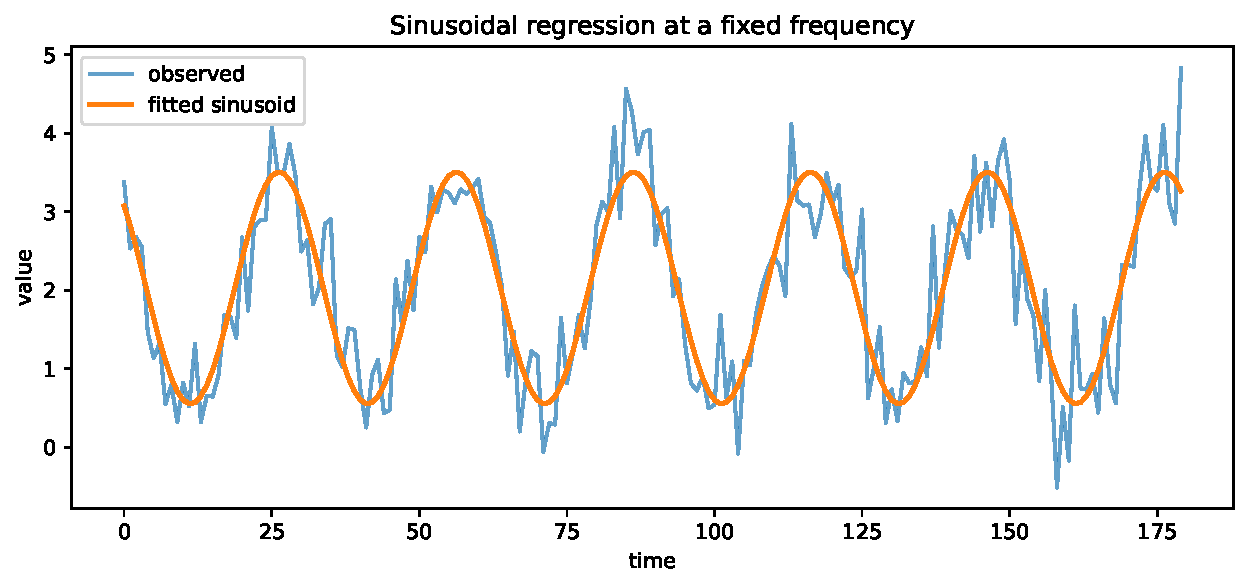
\includegraphics[keepaspectratio]{chapters/chapter-12-spectral-analysis-frequency-domain_files/figure-pdf/ch12-sinusoid-regression-output-2.pdf}}

}

\caption{Fitting a sinusoidal component by linear regression.}

\end{figure}%

\section{12.3 Aliasing in discrete
time}\label{aliasing-in-discrete-time}

In continuous time, many different frequencies can be observed. In
discrete time, we only observe the signal at integer times. This creates
an important phenomenon called \textbf{aliasing}.

For integer \(t\),

\[
\cos(2\pi \omega t)=\cos(2\pi (1-\omega)t).
\]

Therefore frequencies \(\omega\) and \(1-\omega\) generate the same
observed cosine sequence at integer times. For example, \(\omega=0.25\)
and \(\omega=0.75\) are indistinguishable if the data are observed only
at \(t=0,1,2,\ldots\).

Because of aliasing, we usually restrict attention to the fundamental
range

\[
-\frac{1}{2}<\omega\leq \frac{1}{2},
\]

or equivalently

\[
0\leq \omega\leq \frac{1}{2}
\]

for one-sided plots of real-valued data. The frequency \(1/2\) is the
\textbf{Nyquist frequency}.

\begin{tcolorbox}[enhanced jigsaw, arc=.35mm, bottomrule=.15mm, bottomtitle=1mm, breakable, colback=white, colbacktitle=quarto-callout-warning-color!10!white, colframe=quarto-callout-warning-color-frame, coltitle=black, left=2mm, leftrule=.75mm, opacityback=0, opacitybacktitle=0.6, rightrule=.15mm, title=\textcolor{quarto-callout-warning-color}{\faExclamationTriangle}\hspace{0.5em}{Aliasing warning}, titlerule=0mm, toprule=.15mm, toptitle=1mm]

A high-frequency continuous signal can look like a lower-frequency
discrete sequence when sampled too slowly. Spectral analysis always
depends on the sampling rate.

\end{tcolorbox}

\begin{Shaded}
\begin{Highlighting}[]
\NormalTok{fine }\OperatorTok{=}\NormalTok{ np.linspace(}\DecValTok{0}\NormalTok{, }\DecValTok{8}\NormalTok{, }\DecValTok{1000}\NormalTok{)}
\NormalTok{obs }\OperatorTok{=}\NormalTok{ np.arange(}\DecValTok{0}\NormalTok{, }\DecValTok{9}\NormalTok{)}

\NormalTok{w1 }\OperatorTok{=} \FloatTok{0.25}
\NormalTok{w2 }\OperatorTok{=} \FloatTok{0.75}

\NormalTok{plt.figure(figsize}\OperatorTok{=}\NormalTok{(}\DecValTok{10}\NormalTok{, }\DecValTok{4}\NormalTok{))}
\NormalTok{plt.plot(fine, np.cos(}\DecValTok{2}\OperatorTok{*}\NormalTok{np.pi}\OperatorTok{*}\NormalTok{w1}\OperatorTok{*}\NormalTok{fine), label}\OperatorTok{=}\VerbatimStringTok{r"}\DecValTok{$}\ErrorTok{\textbackslash{}}\VerbatimStringTok{omega=0}\DecValTok{.}\VerbatimStringTok{25}\DecValTok{$}\VerbatimStringTok{"}\NormalTok{)}
\NormalTok{plt.plot(fine, np.cos(}\DecValTok{2}\OperatorTok{*}\NormalTok{np.pi}\OperatorTok{*}\NormalTok{w2}\OperatorTok{*}\NormalTok{fine), }\StringTok{"{-}{-}"}\NormalTok{, label}\OperatorTok{=}\VerbatimStringTok{r"}\DecValTok{$}\ErrorTok{\textbackslash{}}\VerbatimStringTok{omega=0}\DecValTok{.}\VerbatimStringTok{75}\DecValTok{$}\VerbatimStringTok{"}\NormalTok{)}
\NormalTok{plt.scatter(obs, np.cos(}\DecValTok{2}\OperatorTok{*}\NormalTok{np.pi}\OperatorTok{*}\NormalTok{w1}\OperatorTok{*}\NormalTok{obs), zorder}\OperatorTok{=}\DecValTok{3}\NormalTok{, label}\OperatorTok{=}\StringTok{"integer samples"}\NormalTok{)}
\NormalTok{plt.xlabel(}\StringTok{"time"}\NormalTok{)}
\NormalTok{plt.ylabel(}\StringTok{"cosine value"}\NormalTok{)}
\NormalTok{plt.title(}\StringTok{"Aliasing in discrete{-}time observations"}\NormalTok{)}
\NormalTok{plt.legend()}
\NormalTok{plt.show()}
\end{Highlighting}
\end{Shaded}

\begin{figure}[H]

{\centering \pandocbounded{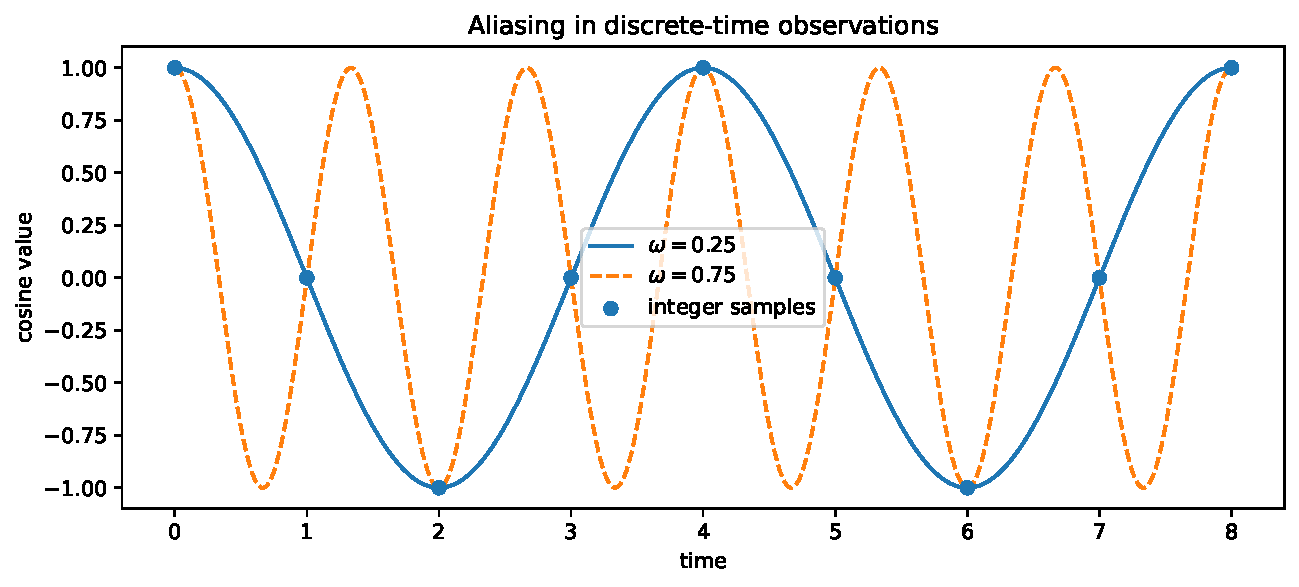
\includegraphics[keepaspectratio]{chapters/chapter-12-spectral-analysis-frequency-domain_files/figure-pdf/ch12-aliasing-example-output-1.pdf}}

}

\caption{Aliasing: two different continuous frequencies agree at integer
time points.}

\end{figure}%

\section{12.4 Random sinusoidal
processes}\label{random-sinusoidal-processes}

A deterministic sinusoid is not a typical stationary stochastic process.
However, randomizing the coefficients gives a useful stationary model.

Let

\[
X_t=A\cos(2\pi\omega t)+B\sin(2\pi\omega t),
\]

where

\[
E[A]=E[B]=0,
\qquad
\operatorname{Var}(A)=\operatorname{Var}(B)=\sigma^2,
\qquad
\operatorname{Cov}(A,B)=0.
\]

Then

\[
E[X_t]=0.
\]

For lag \(h\),

\[
\begin{aligned}
\gamma(h)
&=\operatorname{Cov}(X_{t+h},X_t) \\
&=E[X_{t+h}X_t] \\
&=\sigma^2\cos(2\pi\omega h).
\end{aligned}
\]

Thus \(\gamma(h)\) depends only on the lag \(h\), not on time \(t\).
Therefore \(\{X_t\}\) is weakly stationary.

\begin{tcolorbox}[enhanced jigsaw, arc=.35mm, bottomrule=.15mm, bottomtitle=1mm, breakable, colback=white, colbacktitle=quarto-callout-tip-color!10!white, colframe=quarto-callout-tip-color-frame, coltitle=black, left=2mm, leftrule=.75mm, opacityback=0, opacitybacktitle=0.6, rightrule=.15mm, title=\textcolor{quarto-callout-tip-color}{\faLightbulb}\hspace{0.5em}{Why random coefficients matter}, titlerule=0mm, toprule=.15mm, toptitle=1mm]

A deterministic cosine has a time-varying mean. A random-amplitude
cosine with zero-mean coefficients has constant mean and lag-only
covariance. This is one reason random sinusoidal representations are
natural in stationary time-series theory.

\end{tcolorbox}

More generally, let

\[
X_t=\sum_{j=1}^m \left[A_j\cos(2\pi\omega_j t)+B_j\sin(2\pi\omega_j t)\right],
\]

where the coefficients are uncorrelated, have mean zero, and satisfy

\[
\operatorname{Var}(A_j)=\operatorname{Var}(B_j)=\sigma_j^2.
\]

Then

\[
\gamma(h)=\sum_{j=1}^m \sigma_j^2\cos(2\pi\omega_j h).
\]

The autocovariance function is a sum of cosines. Each frequency
contributes part of the variance.

\section{12.5 Autocovariance and spectral
representation}\label{autocovariance-and-spectral-representation}

For a stationary process, the autocovariance function is

\[
\gamma(h)=\operatorname{Cov}(X_{t+h},X_t).
\]

The spectral representation theorem says that there exists a unique
nondecreasing function \(F\) on \([-1/2,1/2]\), called the
\textbf{spectral distribution function}, such that

\[
\gamma(h)=\int_{-1/2}^{1/2} e^{2\pi i\omega h}\,dF(\omega).
\]

The total mass of \(F\) is

\[
F(1/2)-F(-1/2)=\gamma(0)=\operatorname{Var}(X_t).
\]

This result is the frequency-domain analogue of saying that covariance
matrices must be positive semidefinite. The function \(F\) distributes
the variance of the process across frequencies.

\subsection{Discrete spectral
components}\label{discrete-spectral-components}

For a random sinusoidal process, the spectral distribution has jumps at
the sinusoidal frequencies. A process with a strong deterministic or
nearly deterministic periodic component often produces sharp spectral
peaks.

\subsection{Continuous spectral
components}\label{continuous-spectral-components}

For ARMA-type processes, the spectral distribution is usually
continuous. In this case we can write

\[
dF(\omega)=f(\omega)d\omega,
\]

where \(f\) is the \textbf{spectral density}.

\section{12.6 Spectral density}\label{spectral-density}

If the autocovariance function is absolutely summable,

\[
\sum_{h=-\infty}^{\infty}|\gamma(h)|<\infty,
\]

then the spectral density is defined by the Fourier series

\[
f(\omega)=\sum_{h=-\infty}^{\infty}\gamma(h)e^{-2\pi i\omega h},
\qquad -\frac{1}{2}<\omega<\frac{1}{2}.
\]

The inverse relation is

\[
\gamma(h)=\int_{-1/2}^{1/2}e^{2\pi i\omega h}f(\omega)\,d\omega.
\]

At \(h=0\),

\[
\gamma(0)=\operatorname{Var}(X_t)=\int_{-1/2}^{1/2}f(\omega)\,d\omega.
\]

This identity gives the most important interpretation:

\begin{tcolorbox}[enhanced jigsaw, arc=.35mm, bottomrule=.15mm, bottomtitle=1mm, breakable, colback=white, colbacktitle=quarto-callout-note-color!10!white, colframe=quarto-callout-note-color-frame, coltitle=black, left=2mm, leftrule=.75mm, opacityback=0, opacitybacktitle=0.6, rightrule=.15mm, title=\textcolor{quarto-callout-note-color}{\faInfo}\hspace{0.5em}{Interpretation of the spectral density}, titlerule=0mm, toprule=.15mm, toptitle=1mm]

The spectral density \(f(\omega)\) describes how the variance of a
stationary time series is distributed over frequencies. Large
\(f(\omega)\) means that oscillations near frequency \(\omega\) explain
a relatively large amount of variation.

\end{tcolorbox}

\subsection{Basic properties}\label{basic-properties}

For a real-valued stationary process with absolutely summable
autocovariance:

\begin{enumerate}
\def\labelenumi{\arabic{enumi}.}
\tightlist
\item
  \(f(\omega)\geq 0\);
\item
  \(f(\omega)=f(-\omega)\);
\item
  \(f(\omega+1)=f(\omega)\);
\item
  \(f\) completely determines \(\gamma\);
\item
  for a Gaussian stationary process, \(f\) determines the full
  finite-dimensional distributions.
\end{enumerate}

The evenness \(f(\omega)=f(-\omega)\) means that real-valued processes
have symmetric spectra.

\section{12.7 Interactive spectral
explorer}\label{interactive-spectral-explorer}

The following interactive demonstration combines two sinusoidal
components with noise. Move the frequency, amplitude, and noise sliders.
Notice that the time plot can look complicated, but the spectrum often
reveals the hidden frequencies.

Frequency 1 \(\omega_1\) Amplitude 1 Frequency 2 \(\omega_2\) Amplitude
2 Noise level

\protect\phantomsection\label{ch12_signal_plot}

\protect\phantomsection\label{ch12_spectrum_plot}

The spectrum shown here is a simple finite-sample periodogram-style
display. Chapter 13 develops the DFT, FFT, and periodogram carefully.

\section{12.8 White noise spectrum}\label{white-noise-spectrum}

Let \(W_t\sim WN(0,\sigma^2)\). Then

\[
\gamma(h)=\begin{cases}
\sigma^2, & h=0,\\
0, & h\neq 0.
\end{cases}
\]

Therefore

\[
f(\omega)=\sum_{h=-\infty}^{\infty}\gamma(h)e^{-2\pi i\omega h}=\sigma^2.
\]

White noise has a flat spectrum. Every frequency contributes equally.
This explains the term \textbf{white} noise: it is analogous to white
light, which contains all visible frequencies.

\begin{Shaded}
\begin{Highlighting}[]
\ImportTok{from}\NormalTok{ scipy.signal }\ImportTok{import}\NormalTok{ periodogram}

\NormalTok{rng }\OperatorTok{=}\NormalTok{ np.random.default\_rng(}\DecValTok{2026}\NormalTok{)}
\NormalTok{n }\OperatorTok{=} \DecValTok{512}
\NormalTok{w }\OperatorTok{=}\NormalTok{ rng.normal(}\DecValTok{0}\NormalTok{, }\DecValTok{1}\NormalTok{, size}\OperatorTok{=}\NormalTok{n)}
\NormalTok{freqs, power }\OperatorTok{=}\NormalTok{ periodogram(w, scaling}\OperatorTok{=}\StringTok{"density"}\NormalTok{)}

\NormalTok{plt.figure(figsize}\OperatorTok{=}\NormalTok{(}\DecValTok{10}\NormalTok{, }\DecValTok{4}\NormalTok{))}
\NormalTok{plt.plot(freqs, power)}
\NormalTok{plt.xlabel(}\StringTok{"frequency"}\NormalTok{)}
\NormalTok{plt.ylabel(}\StringTok{"periodogram"}\NormalTok{)}
\NormalTok{plt.title(}\StringTok{"A finite{-}sample spectrum of white noise"}\NormalTok{)}
\NormalTok{plt.show()}
\end{Highlighting}
\end{Shaded}

\begin{figure}[H]

{\centering \pandocbounded{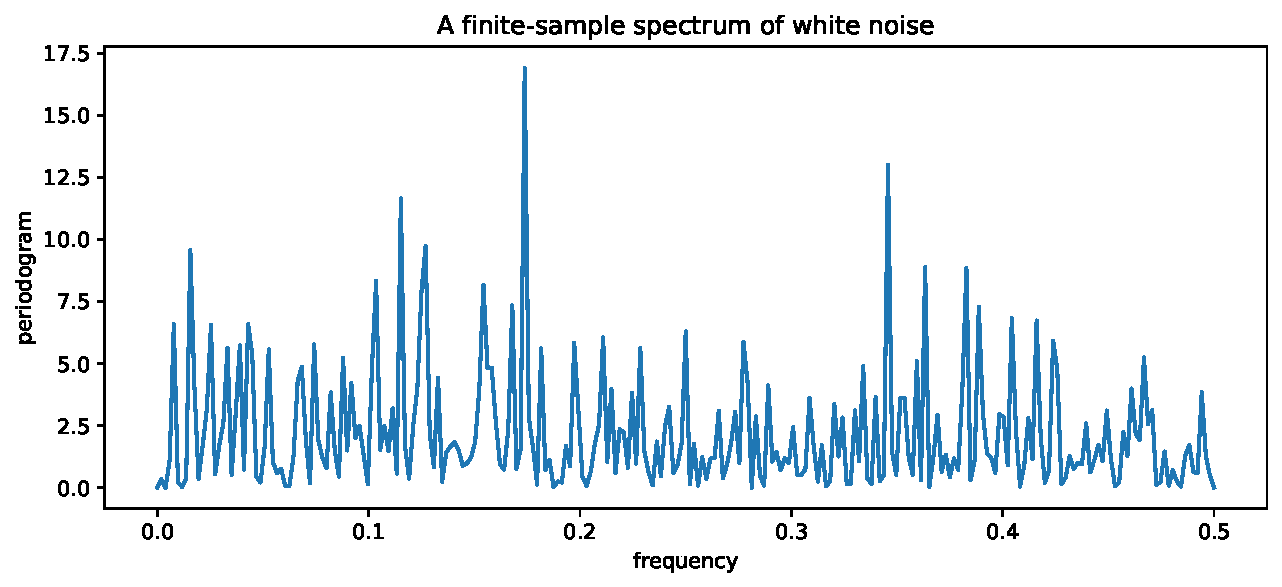
\includegraphics[keepaspectratio]{chapters/chapter-12-spectral-analysis-frequency-domain_files/figure-pdf/ch12-white-noise-spectrum-output-1.pdf}}

}

\caption{White noise has approximately flat spectral power, up to
sampling variability.}

\end{figure}%

The periodogram fluctuates substantially even for white noise. This is
not a contradiction. The flat spectrum is a population statement.
Chapter 13 explains why raw periodograms are noisy and why smoothing is
often needed.

\section{12.9 AR(1) spectrum}\label{ar1-spectrum}

Consider the causal AR(1) model

\[
X_t=\phi X_{t-1}+W_t,
\qquad |\phi|<1,
\qquad W_t\sim WN(0,\sigma^2).
\]

The autocovariance is

\[
\gamma(h)=\frac{\sigma^2\phi^{|h|}}{1-\phi^2}.
\]

Its spectral density is

\[
f(\omega)=\frac{\sigma^2}{1-2\phi\cos(2\pi\omega)+\phi^2}.
\]

This formula has a useful interpretation:

\begin{itemize}
\tightlist
\item
  If \(\phi>0\), nearby observations tend to have the same sign. The
  process is smooth. The spectrum is largest near \(\omega=0\), a low
  frequency.
\item
  If \(\phi<0\), nearby observations tend to alternate signs. The
  process is rough. The spectrum is largest near \(\omega=1/2\), a high
  frequency.
\end{itemize}

AR(1) coefficient \(\phi\)
\protect\phantomsection\label{ch12_phi_label}{}

\protect\phantomsection\label{ch12_ar1_time}

\protect\phantomsection\label{ch12_ar1_spec}

\begin{Shaded}
\begin{Highlighting}[]
\NormalTok{omega\_grid }\OperatorTok{=}\NormalTok{ np.linspace(}\DecValTok{0}\NormalTok{, }\FloatTok{0.5}\NormalTok{, }\DecValTok{400}\NormalTok{)}

\KeywordTok{def}\NormalTok{ ar1\_spectrum(phi, sigma2}\OperatorTok{=}\FloatTok{1.0}\NormalTok{):}
    \ControlFlowTok{return}\NormalTok{ sigma2 }\OperatorTok{/}\NormalTok{ (}\DecValTok{1} \OperatorTok{{-}} \DecValTok{2}\OperatorTok{*}\NormalTok{phi}\OperatorTok{*}\NormalTok{np.cos(}\DecValTok{2}\OperatorTok{*}\NormalTok{np.pi}\OperatorTok{*}\NormalTok{omega\_grid) }\OperatorTok{+}\NormalTok{ phi}\OperatorTok{**}\DecValTok{2}\NormalTok{)}

\NormalTok{plt.figure(figsize}\OperatorTok{=}\NormalTok{(}\DecValTok{10}\NormalTok{, }\DecValTok{4}\NormalTok{))}
\NormalTok{plt.plot(omega\_grid, ar1\_spectrum(}\FloatTok{0.9}\NormalTok{), label}\OperatorTok{=}\VerbatimStringTok{r"}\DecValTok{$}\ErrorTok{\textbackslash{}}\VerbatimStringTok{phi=0}\DecValTok{.}\VerbatimStringTok{9}\DecValTok{$}\VerbatimStringTok{"}\NormalTok{)}
\NormalTok{plt.plot(omega\_grid, ar1\_spectrum(}\OperatorTok{{-}}\FloatTok{0.9}\NormalTok{), label}\OperatorTok{=}\VerbatimStringTok{r"}\DecValTok{$}\ErrorTok{\textbackslash{}}\VerbatimStringTok{phi={-}0}\DecValTok{.}\VerbatimStringTok{9}\DecValTok{$}\VerbatimStringTok{"}\NormalTok{)}
\NormalTok{plt.xlabel(}\StringTok{"frequency"}\NormalTok{)}
\NormalTok{plt.ylabel(}\StringTok{"spectral density"}\NormalTok{)}
\NormalTok{plt.title(}\StringTok{"AR(1) spectra"}\NormalTok{)}
\NormalTok{plt.legend()}
\NormalTok{plt.show()}
\end{Highlighting}
\end{Shaded}

\begin{figure}[H]

{\centering \pandocbounded{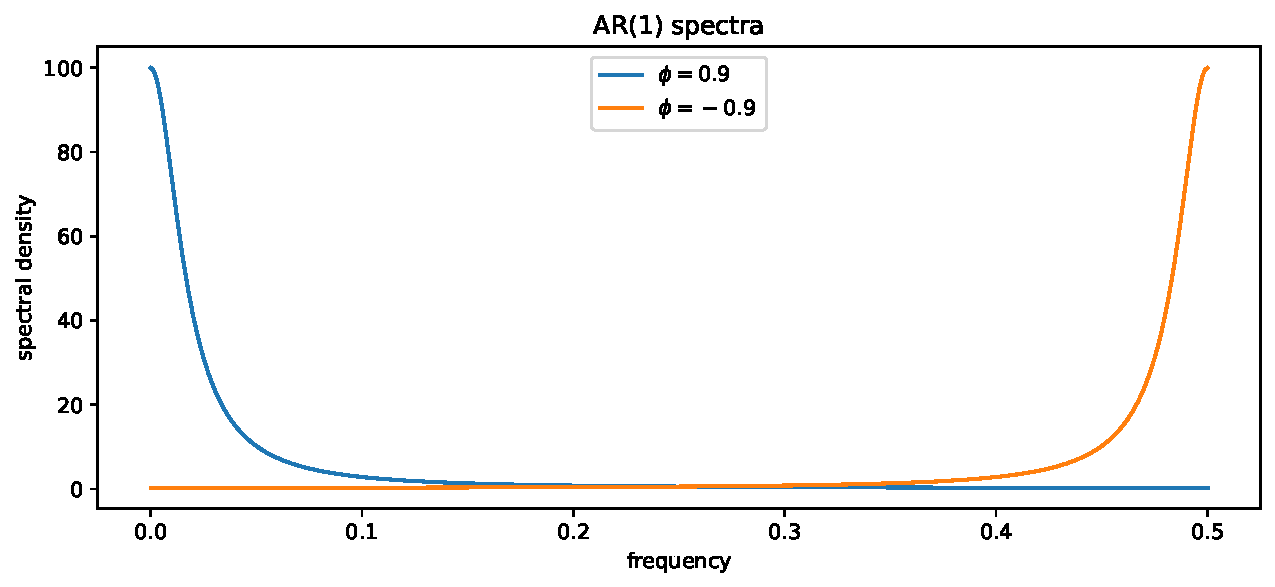
\includegraphics[keepaspectratio]{chapters/chapter-12-spectral-analysis-frequency-domain_files/figure-pdf/ch12-ar1-spectra-output-1.pdf}}

}

\caption{Theoretical spectral densities for positive and negative AR(1)
coefficients.}

\end{figure}%

\section{12.10 MA(1) spectrum}\label{ma1-spectrum}

Consider the MA(1) model

\[
X_t=W_t+\theta W_{t-1},
\qquad W_t\sim WN(0,\sigma^2).
\]

The autocovariance is

\[
\gamma(h)=\begin{cases}
\sigma^2(1+\theta^2), & h=0,\\
\sigma^2\theta, & |h|=1,\\
0, & |h|>1.
\end{cases}
\]

Therefore

\[
\begin{aligned}
f(\omega)
&=\gamma(0)+\gamma(1)e^{-2\pi i\omega}+\gamma(-1)e^{2\pi i\omega}\\
&=\sigma^2(1+\theta^2)+2\sigma^2\theta\cos(2\pi\omega)\\
&=\sigma^2\left|1+\theta e^{-2\pi i\omega}\right|^2.
\end{aligned}
\]

If \(\theta>0\), the spectrum is larger at low frequencies. If
\(\theta<0\), it is larger near the Nyquist frequency.

\begin{Shaded}
\begin{Highlighting}[]
\KeywordTok{def}\NormalTok{ ma1\_spectrum(theta, sigma2}\OperatorTok{=}\FloatTok{1.0}\NormalTok{):}
    \ControlFlowTok{return}\NormalTok{ sigma2 }\OperatorTok{*}\NormalTok{ (}\DecValTok{1} \OperatorTok{+}\NormalTok{ theta}\OperatorTok{**}\DecValTok{2} \OperatorTok{+} \DecValTok{2}\OperatorTok{*}\NormalTok{theta}\OperatorTok{*}\NormalTok{np.cos(}\DecValTok{2}\OperatorTok{*}\NormalTok{np.pi}\OperatorTok{*}\NormalTok{omega\_grid))}

\NormalTok{plt.figure(figsize}\OperatorTok{=}\NormalTok{(}\DecValTok{10}\NormalTok{, }\DecValTok{4}\NormalTok{))}
\NormalTok{plt.plot(omega\_grid, ma1\_spectrum(}\FloatTok{0.9}\NormalTok{), label}\OperatorTok{=}\VerbatimStringTok{r"}\DecValTok{$}\CharTok{\textbackslash{}t}\VerbatimStringTok{heta=0}\DecValTok{.}\VerbatimStringTok{9}\DecValTok{$}\VerbatimStringTok{"}\NormalTok{)}
\NormalTok{plt.plot(omega\_grid, ma1\_spectrum(}\OperatorTok{{-}}\FloatTok{0.9}\NormalTok{), label}\OperatorTok{=}\VerbatimStringTok{r"}\DecValTok{$}\CharTok{\textbackslash{}t}\VerbatimStringTok{heta={-}0}\DecValTok{.}\VerbatimStringTok{9}\DecValTok{$}\VerbatimStringTok{"}\NormalTok{)}
\NormalTok{plt.xlabel(}\StringTok{"frequency"}\NormalTok{)}
\NormalTok{plt.ylabel(}\StringTok{"spectral density"}\NormalTok{)}
\NormalTok{plt.title(}\StringTok{"MA(1) spectra"}\NormalTok{)}
\NormalTok{plt.legend()}
\NormalTok{plt.show()}
\end{Highlighting}
\end{Shaded}

\begin{figure}[H]

{\centering \pandocbounded{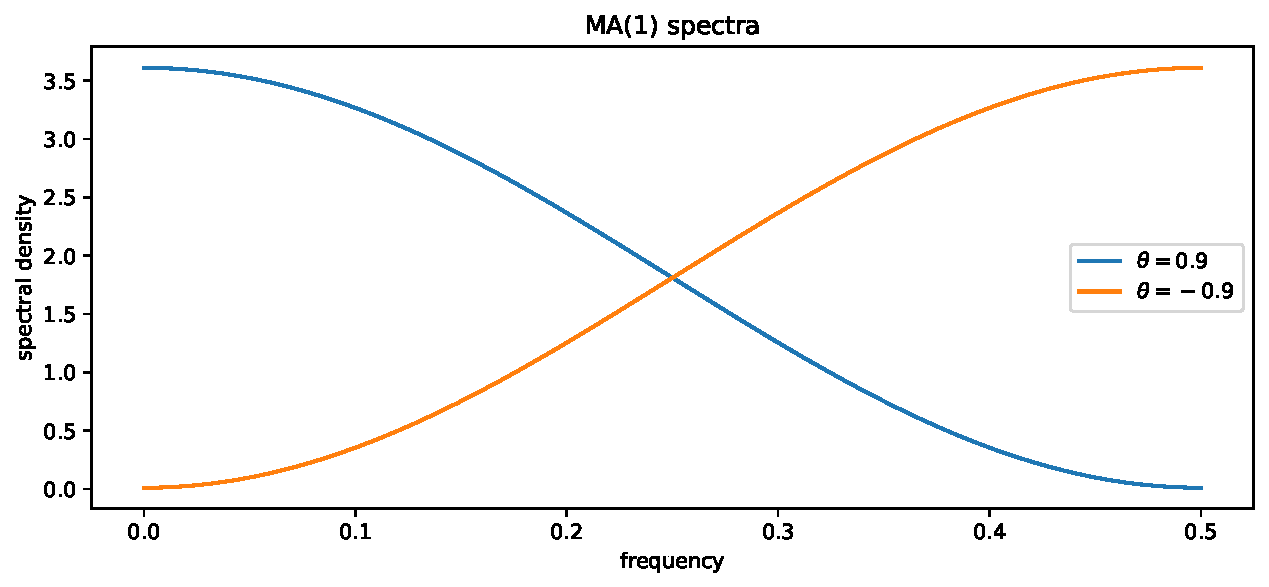
\includegraphics[keepaspectratio]{chapters/chapter-12-spectral-analysis-frequency-domain_files/figure-pdf/ch12-ma1-spectra-output-1.pdf}}

}

\caption{Theoretical spectral densities for positive and negative MA(1)
coefficients.}

\end{figure}%

\section{12.11 Spectral density of a causal ARMA
process}\label{spectral-density-of-a-causal-arma-process}

Let \(X_t\) be a causal ARMA(\(p,q\)) process:

\[
\phi(B)X_t=\theta(B)W_t,
\qquad W_t\sim WN(0,\sigma^2),
\]

where

\[
\phi(B)=1-\phi_1B-\cdots-\phi_pB^p,
\]

and

\[
\theta(B)=1+\theta_1B+\cdots+\theta_qB^q.
\]

Causality gives the linear-process representation

\[
X_t=\psi(B)W_t,
\qquad
\psi(B)=\frac{\theta(B)}{\phi(B)}.
\]

The spectral density is

\[
f(\omega)
=\sigma^2\left|\psi(e^{-2\pi i\omega})\right|^2
=\sigma^2\frac{\left|\theta(e^{-2\pi i\omega})\right|^2}
{\left|\phi(e^{-2\pi i\omega})\right|^2}.
\]

This formula is one of the main reasons spectral analysis is useful.
ARMA models become simple frequency filters applied to white noise.

\begin{tcolorbox}[enhanced jigsaw, arc=.35mm, bottomrule=.15mm, bottomtitle=1mm, breakable, colback=white, colbacktitle=quarto-callout-note-color!10!white, colframe=quarto-callout-note-color-frame, coltitle=black, left=2mm, leftrule=.75mm, opacityback=0, opacitybacktitle=0.6, rightrule=.15mm, title=\textcolor{quarto-callout-note-color}{\faInfo}\hspace{0.5em}{ARMA as filtered white noise}, titlerule=0mm, toprule=.15mm, toptitle=1mm]

White noise has a flat spectrum. A causal ARMA model reshapes this flat
spectrum by multiplying it by

\[
\left|\frac{\theta(e^{-2\pi i\omega})}{\phi(e^{-2\pi i\omega})}\right|^2.
\]

The AR polynomial can amplify frequencies near its roots, while the MA
polynomial can suppress or amplify frequencies depending on its zeros.

\end{tcolorbox}

\begin{Shaded}
\begin{Highlighting}[]
\ImportTok{import}\NormalTok{ numpy.polynomial.polynomial }\ImportTok{as}\NormalTok{ poly}

\KeywordTok{def}\NormalTok{ arma\_spectrum(ar\_coefs, ma\_coefs, sigma2}\OperatorTok{=}\FloatTok{1.0}\NormalTok{, grid}\OperatorTok{=}\VariableTok{None}\NormalTok{):}
    \CommentTok{"""}
\CommentTok{    ar\_coefs: [phi\_1, ..., phi\_p] for phi(B)=1 {-} phi\_1 B {-} ... {-} phi\_p B\^{}p}
\CommentTok{    ma\_coefs: [theta\_1, ..., theta\_q] for theta(B)=1 + theta\_1 B + ... + theta\_q B\^{}q}
\CommentTok{    """}
    \ControlFlowTok{if}\NormalTok{ grid }\KeywordTok{is} \VariableTok{None}\NormalTok{:}
\NormalTok{        grid }\OperatorTok{=}\NormalTok{ np.linspace(}\DecValTok{0}\NormalTok{, }\FloatTok{0.5}\NormalTok{, }\DecValTok{400}\NormalTok{)}
\NormalTok{    z }\OperatorTok{=}\NormalTok{ np.exp(}\OperatorTok{{-}}\OtherTok{2j} \OperatorTok{*}\NormalTok{ np.pi }\OperatorTok{*}\NormalTok{ grid)}
\NormalTok{    theta }\OperatorTok{=}\NormalTok{ np.ones\_like(z, dtype}\OperatorTok{=}\BuiltInTok{complex}\NormalTok{)}
    \ControlFlowTok{for}\NormalTok{ j, coef }\KeywordTok{in} \BuiltInTok{enumerate}\NormalTok{(ma\_coefs, start}\OperatorTok{=}\DecValTok{1}\NormalTok{):}
\NormalTok{        theta }\OperatorTok{+=}\NormalTok{ coef }\OperatorTok{*}\NormalTok{ z}\OperatorTok{**}\NormalTok{j}
\NormalTok{    phi }\OperatorTok{=}\NormalTok{ np.ones\_like(z, dtype}\OperatorTok{=}\BuiltInTok{complex}\NormalTok{)}
    \ControlFlowTok{for}\NormalTok{ j, coef }\KeywordTok{in} \BuiltInTok{enumerate}\NormalTok{(ar\_coefs, start}\OperatorTok{=}\DecValTok{1}\NormalTok{):}
\NormalTok{        phi }\OperatorTok{{-}=}\NormalTok{ coef }\OperatorTok{*}\NormalTok{ z}\OperatorTok{**}\NormalTok{j}
    \ControlFlowTok{return}\NormalTok{ grid, sigma2 }\OperatorTok{*}\NormalTok{ np.}\BuiltInTok{abs}\NormalTok{(theta)}\OperatorTok{**}\DecValTok{2} \OperatorTok{/}\NormalTok{ np.}\BuiltInTok{abs}\NormalTok{(phi)}\OperatorTok{**}\DecValTok{2}

\NormalTok{freq, spec\_a }\OperatorTok{=}\NormalTok{ arma\_spectrum(ar\_coefs}\OperatorTok{=}\NormalTok{[}\FloatTok{1.2}\NormalTok{, }\OperatorTok{{-}}\FloatTok{0.7}\NormalTok{], ma\_coefs}\OperatorTok{=}\NormalTok{[}\FloatTok{0.4}\NormalTok{])}
\NormalTok{freq, spec\_b }\OperatorTok{=}\NormalTok{ arma\_spectrum(ar\_coefs}\OperatorTok{=}\NormalTok{[}\FloatTok{0.8}\NormalTok{], ma\_coefs}\OperatorTok{=}\NormalTok{[}\OperatorTok{{-}}\FloatTok{0.8}\NormalTok{])}

\NormalTok{plt.figure(figsize}\OperatorTok{=}\NormalTok{(}\DecValTok{10}\NormalTok{, }\DecValTok{4}\NormalTok{))}
\NormalTok{plt.plot(freq, spec\_a, label}\OperatorTok{=}\StringTok{"ARMA(2,1)"}\NormalTok{)}
\NormalTok{plt.plot(freq, spec\_b, label}\OperatorTok{=}\StringTok{"ARMA(1,1)"}\NormalTok{)}
\NormalTok{plt.xlabel(}\StringTok{"frequency"}\NormalTok{)}
\NormalTok{plt.ylabel(}\StringTok{"spectral density"}\NormalTok{)}
\NormalTok{plt.title(}\StringTok{"ARMA spectra from polynomial ratios"}\NormalTok{)}
\NormalTok{plt.legend()}
\NormalTok{plt.show()}
\end{Highlighting}
\end{Shaded}

\begin{figure}[H]

{\centering \pandocbounded{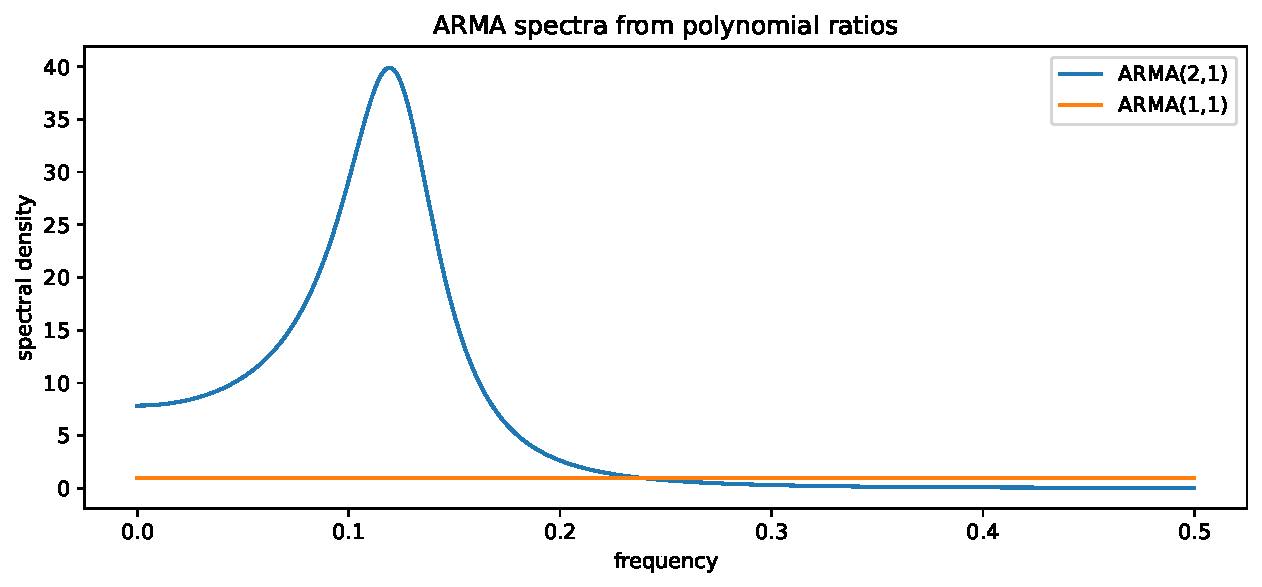
\includegraphics[keepaspectratio]{chapters/chapter-12-spectral-analysis-frequency-domain_files/figure-pdf/ch12-arma-spectrum-function-output-1.pdf}}

}

\caption{ARMA spectral density computed from the AR and MA polynomials.}

\end{figure}%

\section{12.12 Low frequency, high frequency, and time-domain
appearance}\label{low-frequency-high-frequency-and-time-domain-appearance}

The shape of a spectrum has direct time-domain meaning.

\subsection{Low-frequency dominance}\label{low-frequency-dominance}

A series dominated by low frequencies changes slowly. It may look
smooth, persistent, or trend-like over short windows. Positive AR
coefficients often create strong low-frequency power.

\subsection{High-frequency dominance}\label{high-frequency-dominance}

A series dominated by high frequencies changes direction quickly. It may
look jagged or alternating. Negative AR coefficients and negative MA
coefficients can create high-frequency power.

\subsection{Narrow spectral peaks}\label{narrow-spectral-peaks}

A narrow peak indicates a strong oscillation near a particular period.
For example, a peak near \(\omega=1/12\) suggests a period of \(12\)
time steps.

\subsection{Broad spectral regions}\label{broad-spectral-regions}

A broad region of elevated spectral density suggests variability spread
over a range of frequencies rather than one clean periodic component.

\begin{Shaded}
\begin{Highlighting}[]
\NormalTok{rng }\OperatorTok{=}\NormalTok{ np.random.default\_rng(}\DecValTok{104}\NormalTok{)}
\NormalTok{n }\OperatorTok{=} \DecValTok{240}
\NormalTok{eps }\OperatorTok{=}\NormalTok{ rng.normal(size}\OperatorTok{=}\NormalTok{n)}

\NormalTok{x\_low }\OperatorTok{=}\NormalTok{ np.zeros(n)}
\NormalTok{x\_high }\OperatorTok{=}\NormalTok{ np.zeros(n)}
\ControlFlowTok{for}\NormalTok{ i }\KeywordTok{in} \BuiltInTok{range}\NormalTok{(}\DecValTok{1}\NormalTok{, n):}
\NormalTok{    x\_low[i] }\OperatorTok{=} \FloatTok{0.9} \OperatorTok{*}\NormalTok{ x\_low[i}\OperatorTok{{-}}\DecValTok{1}\NormalTok{] }\OperatorTok{+}\NormalTok{ eps[i]}
\NormalTok{    x\_high[i] }\OperatorTok{=} \OperatorTok{{-}}\FloatTok{0.9} \OperatorTok{*}\NormalTok{ x\_high[i}\OperatorTok{{-}}\DecValTok{1}\NormalTok{] }\OperatorTok{+}\NormalTok{ eps[i]}

\NormalTok{plt.figure(figsize}\OperatorTok{=}\NormalTok{(}\DecValTok{10}\NormalTok{, }\DecValTok{4}\NormalTok{))}
\NormalTok{plt.plot(x\_low, label}\OperatorTok{=}\VerbatimStringTok{r"low{-}frequency dominated, }\DecValTok{$}\ErrorTok{\textbackslash{}}\VerbatimStringTok{phi=0}\DecValTok{.}\VerbatimStringTok{9}\DecValTok{$}\VerbatimStringTok{"}\NormalTok{)}
\NormalTok{plt.plot(x\_high, label}\OperatorTok{=}\VerbatimStringTok{r"high{-}frequency dominated, }\DecValTok{$}\ErrorTok{\textbackslash{}}\VerbatimStringTok{phi={-}0}\DecValTok{.}\VerbatimStringTok{9}\DecValTok{$}\VerbatimStringTok{"}\NormalTok{, alpha}\OperatorTok{=}\FloatTok{0.8}\NormalTok{)}
\NormalTok{plt.xlabel(}\StringTok{"time"}\NormalTok{)}
\NormalTok{plt.ylabel(}\StringTok{"value"}\NormalTok{)}
\NormalTok{plt.title(}\StringTok{"Time{-}domain appearance of different spectra"}\NormalTok{)}
\NormalTok{plt.legend()}
\NormalTok{plt.show()}
\end{Highlighting}
\end{Shaded}

\begin{figure}[H]

{\centering \pandocbounded{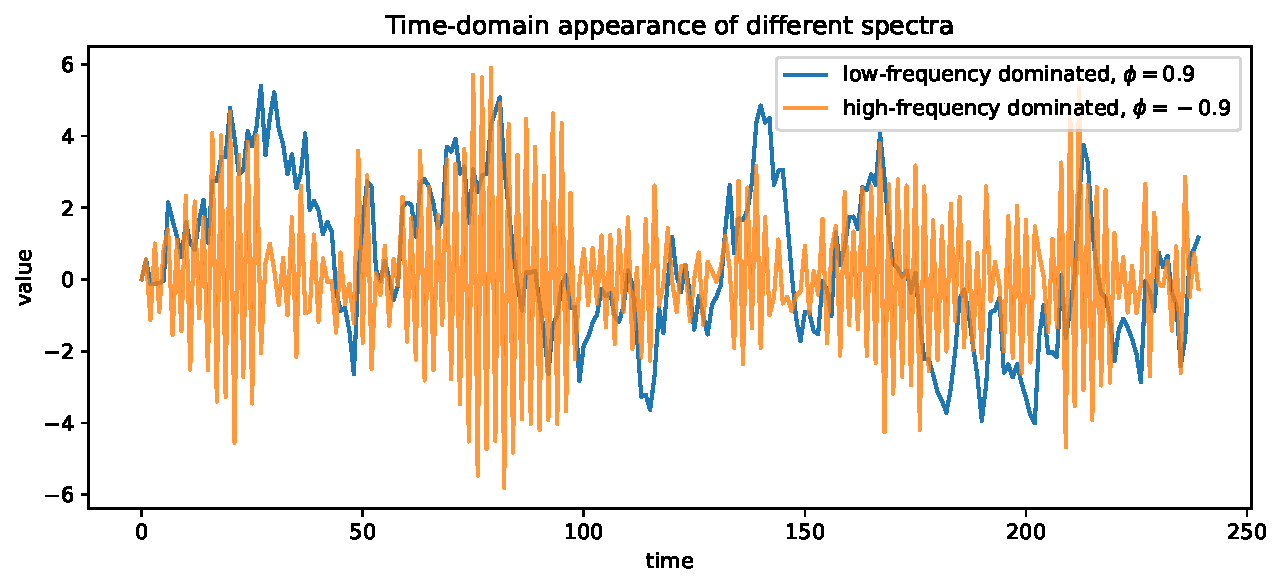
\includegraphics[keepaspectratio]{chapters/chapter-12-spectral-analysis-frequency-domain_files/figure-pdf/ch12-low-high-frequency-simulation-output-1.pdf}}

}

\caption{Low-frequency and high-frequency dominated sequences.}

\end{figure}%

\section{12.13 Spectral analysis and
stationarity}\label{spectral-analysis-and-stationarity}

Classical spectral density is a property of a stationary process. This
matters.

If a series has a deterministic trend, the low-frequency region can be
dominated by the trend. If a series has changing variance, a single
spectrum may average together different regimes. If a series has
changing frequencies over time, a global spectrum may hide the
time-local structure.

A practical workflow is:

\begin{enumerate}
\def\labelenumi{\arabic{enumi}.}
\tightlist
\item
  plot the time series;
\item
  check for trend, seasonality, variance changes, and outliers;
\item
  transform or difference if needed;
\item
  examine the ACF and PACF;
\item
  examine frequency-domain evidence;
\item
  connect spectral features to time-domain models or scientific
  explanations.
\end{enumerate}

\begin{tcolorbox}[enhanced jigsaw, arc=.35mm, bottomrule=.15mm, bottomtitle=1mm, breakable, colback=white, colbacktitle=quarto-callout-warning-color!10!white, colframe=quarto-callout-warning-color-frame, coltitle=black, left=2mm, leftrule=.75mm, opacityback=0, opacitybacktitle=0.6, rightrule=.15mm, title=\textcolor{quarto-callout-warning-color}{\faExclamationTriangle}\hspace{0.5em}{Do not skip EDA}, titlerule=0mm, toprule=.15mm, toptitle=1mm]

A spectral peak is not automatically a meaningful cycle. It may be
caused by trend, sampling artifacts, missing data patterns, calendar
effects, or preprocessing choices.

\end{tcolorbox}

\section{12.14 From spectra to filters}\label{from-spectra-to-filters}

A linear filter transforms a time series into another time series:

\[
Y_t=\sum_{j=-\infty}^{\infty}a_jX_{t-j}.
\]

If \(X_t\) has spectral density \(f_X(\omega)\), then under suitable
summability conditions, \(Y_t\) has spectral density

\[
f_Y(\omega)=|A(\omega)|^2 f_X(\omega),
\]

where

\[
A(\omega)=\sum_{j=-\infty}^{\infty}a_j e^{-2\pi i\omega j}
\]

is the frequency response of the filter.

This explains why moving averages smooth a series: they reduce
high-frequency power. We will return to filters, FFT computation, and
wavelets in Chapters 13 and 14.

\begin{Shaded}
\begin{Highlighting}[]
\NormalTok{omega }\OperatorTok{=}\NormalTok{ np.linspace(}\FloatTok{1e{-}4}\NormalTok{, }\FloatTok{0.5}\NormalTok{, }\DecValTok{500}\NormalTok{)}

\KeywordTok{def}\NormalTok{ ma\_filter\_gain(m):}
\NormalTok{    numerator }\OperatorTok{=}\NormalTok{ np.sin(np.pi }\OperatorTok{*}\NormalTok{ m }\OperatorTok{*}\NormalTok{ omega)}
\NormalTok{    denominator }\OperatorTok{=}\NormalTok{ m }\OperatorTok{*}\NormalTok{ np.sin(np.pi }\OperatorTok{*}\NormalTok{ omega)}
    \ControlFlowTok{return}\NormalTok{ (numerator }\OperatorTok{/}\NormalTok{ denominator)}\OperatorTok{**}\DecValTok{2}

\NormalTok{plt.figure(figsize}\OperatorTok{=}\NormalTok{(}\DecValTok{10}\NormalTok{, }\DecValTok{4}\NormalTok{))}
\ControlFlowTok{for}\NormalTok{ m }\KeywordTok{in}\NormalTok{ [}\DecValTok{3}\NormalTok{, }\DecValTok{7}\NormalTok{, }\DecValTok{15}\NormalTok{]:}
\NormalTok{    plt.plot(omega, ma\_filter\_gain(m), label}\OperatorTok{=}\SpecialStringTok{f"window m=}\SpecialCharTok{\{}\NormalTok{m}\SpecialCharTok{\}}\SpecialStringTok{"}\NormalTok{)}
\NormalTok{plt.xlabel(}\StringTok{"frequency"}\NormalTok{)}
\NormalTok{plt.ylabel(}\VerbatimStringTok{r"}\DecValTok{$}\ControlFlowTok{|}\VerbatimStringTok{A}\KeywordTok{(}\ErrorTok{\textbackslash{}}\VerbatimStringTok{omega}\KeywordTok{)}\ControlFlowTok{|}\DecValTok{\^{}}\VerbatimStringTok{2}\DecValTok{$}\VerbatimStringTok{"}\NormalTok{)}
\NormalTok{plt.title(}\StringTok{"Frequency response of simple moving{-}average filters"}\NormalTok{)}
\NormalTok{plt.legend()}
\NormalTok{plt.show()}
\end{Highlighting}
\end{Shaded}

\begin{figure}[H]

{\centering \pandocbounded{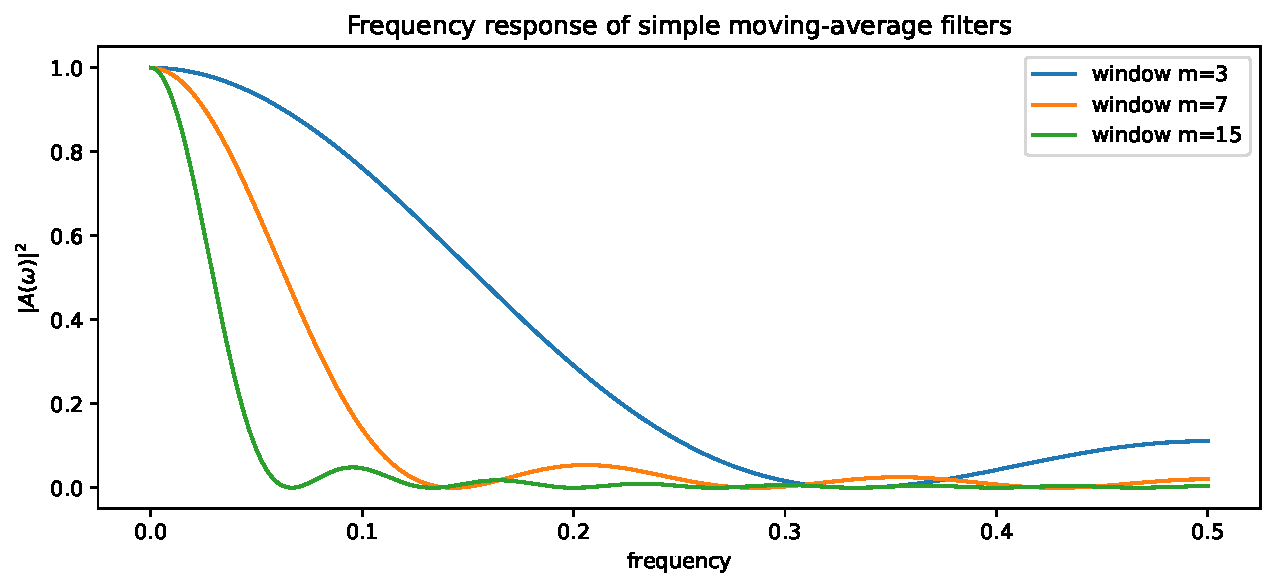
\includegraphics[keepaspectratio]{chapters/chapter-12-spectral-analysis-frequency-domain_files/figure-pdf/ch12-moving-average-filter-spectrum-output-1.pdf}}

}

\caption{A moving-average filter suppresses high frequencies.}

\end{figure}%

\section{12.15 AI-assisted spectral
modeling}\label{ai-assisted-spectral-modeling}

AI tools can be useful for brainstorming explanations of spectral
features, generating code, and checking interpretations. But
frequency-domain analysis is easy to overinterpret. Students should use
AI as a critic, not as an oracle.

\section{AI-assisted study box: spectral interpretation
prompt}\label{ai-assisted-study-box-spectral-interpretation-prompt}

Use the following prompt after producing a time plot, ACF, and spectrum.

\begin{quote}
I have a stationary time series with the following evidence: {[}describe
time plot{]}, {[}describe ACF{]}, {[}describe spectral peaks{]}. Propose
three possible data-generating explanations. For each explanation, state
one mathematical model, one diagnostic that could refute it, and one
possible artifact caused by sampling or preprocessing. Do not choose a
final model until the diagnostics are checked.
\end{quote}

\subsection{Verification checklist for AI
output}\label{verification-checklist-for-ai-output}

When an AI assistant proposes a spectral explanation, verify:

\begin{enumerate}
\def\labelenumi{\arabic{enumi}.}
\tightlist
\item
  \textbf{Frequency-to-period conversion:} if the peak is at \(\omega\),
  the period is \(1/\omega\).
\item
  \textbf{Sampling rate:} the interpretation uses the correct time unit.
\item
  \textbf{Aliasing:} no conclusion relies on a frequency beyond the
  Nyquist limit.
\item
  \textbf{Stationarity:} trend and changing variance were considered.
\item
  \textbf{Model link:} the proposed time-domain model has a spectrum
  consistent with the observed one.
\item
  \textbf{Validation:} forecasting or classification performance is
  checked out of sample.
\end{enumerate}

\section{12.16 Python workflow: from time plot to
spectrum}\label{python-workflow-from-time-plot-to-spectrum}

The following workflow is a template. It simulates a stationary series
with two periodic components and AR noise, then compares the time-domain
and frequency-domain views.

\protect\phantomsection\label{ch12-full-workflow}
\begin{Shaded}
\begin{Highlighting}[]
\ImportTok{from}\NormalTok{ scipy.signal }\ImportTok{import}\NormalTok{ periodogram, welch}
\ImportTok{from}\NormalTok{ statsmodels.tsa.stattools }\ImportTok{import}\NormalTok{ acf}

\NormalTok{rng }\OperatorTok{=}\NormalTok{ np.random.default\_rng(}\DecValTok{8}\NormalTok{)}
\NormalTok{n }\OperatorTok{=} \DecValTok{512}
\NormalTok{t }\OperatorTok{=}\NormalTok{ np.arange(n)}

\CommentTok{\# AR(1) noise}
\NormalTok{eta }\OperatorTok{=}\NormalTok{ rng.normal(scale}\OperatorTok{=}\FloatTok{0.7}\NormalTok{, size}\OperatorTok{=}\NormalTok{n)}
\NormalTok{u }\OperatorTok{=}\NormalTok{ np.zeros(n)}
\ControlFlowTok{for}\NormalTok{ i }\KeywordTok{in} \BuiltInTok{range}\NormalTok{(}\DecValTok{1}\NormalTok{, n):}
\NormalTok{    u[i] }\OperatorTok{=} \FloatTok{0.6} \OperatorTok{*}\NormalTok{ u[i}\OperatorTok{{-}}\DecValTok{1}\NormalTok{] }\OperatorTok{+}\NormalTok{ eta[i]}

\NormalTok{x }\OperatorTok{=} \FloatTok{1.8}\OperatorTok{*}\NormalTok{np.cos(}\DecValTok{2}\OperatorTok{*}\NormalTok{np.pi}\OperatorTok{*}\NormalTok{(}\DecValTok{1}\OperatorTok{/}\DecValTok{32}\NormalTok{)}\OperatorTok{*}\NormalTok{t }\OperatorTok{+} \FloatTok{0.5}\NormalTok{) }\OperatorTok{+} \FloatTok{0.9}\OperatorTok{*}\NormalTok{np.sin(}\DecValTok{2}\OperatorTok{*}\NormalTok{np.pi}\OperatorTok{*}\NormalTok{(}\DecValTok{1}\OperatorTok{/}\DecValTok{8}\NormalTok{)}\OperatorTok{*}\NormalTok{t) }\OperatorTok{+}\NormalTok{ u}

\NormalTok{freq\_p, power\_p }\OperatorTok{=}\NormalTok{ periodogram(x }\OperatorTok{{-}}\NormalTok{ x.mean(), scaling}\OperatorTok{=}\StringTok{"density"}\NormalTok{)}
\NormalTok{freq\_w, power\_w }\OperatorTok{=}\NormalTok{ welch(x }\OperatorTok{{-}}\NormalTok{ x.mean(), nperseg}\OperatorTok{=}\DecValTok{128}\NormalTok{, scaling}\OperatorTok{=}\StringTok{"density"}\NormalTok{)}
\NormalTok{acf\_vals }\OperatorTok{=}\NormalTok{ acf(x, nlags}\OperatorTok{=}\DecValTok{40}\NormalTok{, fft}\OperatorTok{=}\VariableTok{True}\NormalTok{)}

\NormalTok{plt.figure(figsize}\OperatorTok{=}\NormalTok{(}\DecValTok{10}\NormalTok{, }\DecValTok{4}\NormalTok{))}
\NormalTok{plt.plot(t, x)}
\NormalTok{plt.xlabel(}\StringTok{"time"}\NormalTok{)}
\NormalTok{plt.ylabel(}\StringTok{"value"}\NormalTok{)}
\NormalTok{plt.title(}\StringTok{"Time plot"}\NormalTok{)}
\NormalTok{plt.show()}

\NormalTok{plt.figure(figsize}\OperatorTok{=}\NormalTok{(}\DecValTok{10}\NormalTok{, }\DecValTok{4}\NormalTok{))}
\NormalTok{plt.stem(np.arange(}\BuiltInTok{len}\NormalTok{(acf\_vals)), acf\_vals)}
\NormalTok{plt.xlabel(}\StringTok{"lag"}\NormalTok{)}
\NormalTok{plt.ylabel(}\StringTok{"sample ACF"}\NormalTok{)}
\NormalTok{plt.title(}\StringTok{"Sample ACF"}\NormalTok{)}
\NormalTok{plt.show()}

\NormalTok{plt.figure(figsize}\OperatorTok{=}\NormalTok{(}\DecValTok{10}\NormalTok{, }\DecValTok{4}\NormalTok{))}
\NormalTok{plt.plot(freq\_p, power\_p, alpha}\OperatorTok{=}\FloatTok{0.45}\NormalTok{, label}\OperatorTok{=}\StringTok{"raw periodogram"}\NormalTok{)}
\NormalTok{plt.plot(freq\_w, power\_w, linewidth}\OperatorTok{=}\DecValTok{2}\NormalTok{, label}\OperatorTok{=}\StringTok{"Welch smoothed estimate"}\NormalTok{)}
\NormalTok{plt.xlim(}\DecValTok{0}\NormalTok{, }\FloatTok{0.5}\NormalTok{)}
\NormalTok{plt.xlabel(}\StringTok{"frequency"}\NormalTok{)}
\NormalTok{plt.ylabel(}\StringTok{"spectral power"}\NormalTok{)}
\NormalTok{plt.title(}\StringTok{"Frequency{-}domain diagnostics"}\NormalTok{)}
\NormalTok{plt.legend()}
\NormalTok{plt.show()}
\end{Highlighting}
\end{Shaded}

\begin{figure}[H]

{\centering \pandocbounded{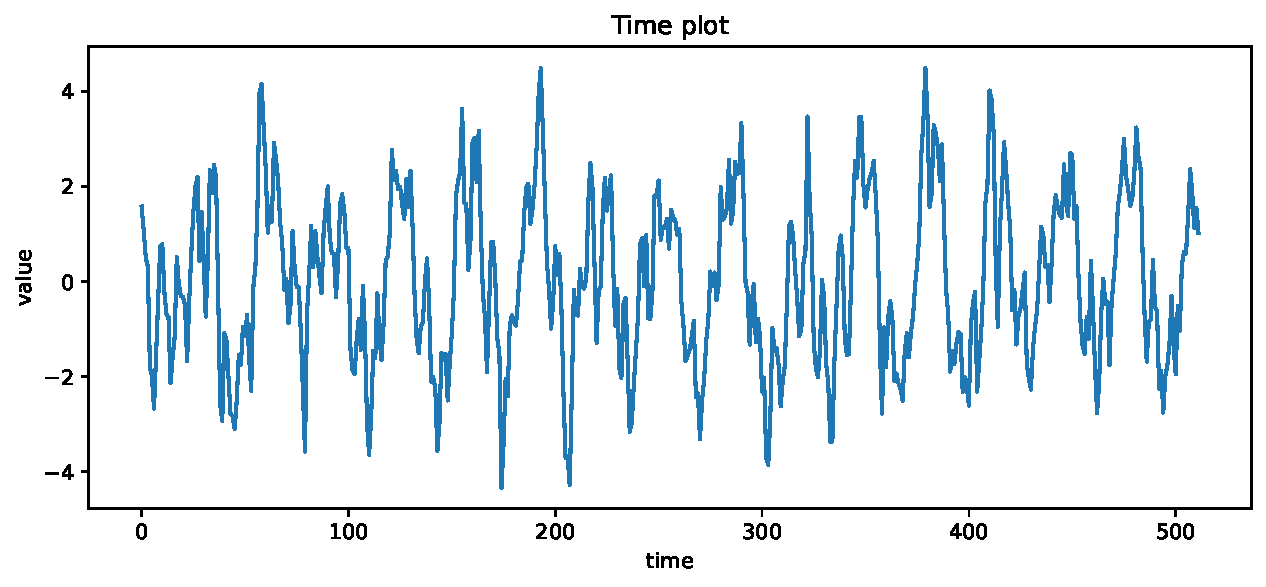
\includegraphics[keepaspectratio]{chapters/chapter-12-spectral-analysis-frequency-domain_files/figure-pdf/ch12-full-workflow-output-1.pdf}}

}

\caption{A complete first spectral workflow for simulated data.}

\end{figure}%

\pandocbounded{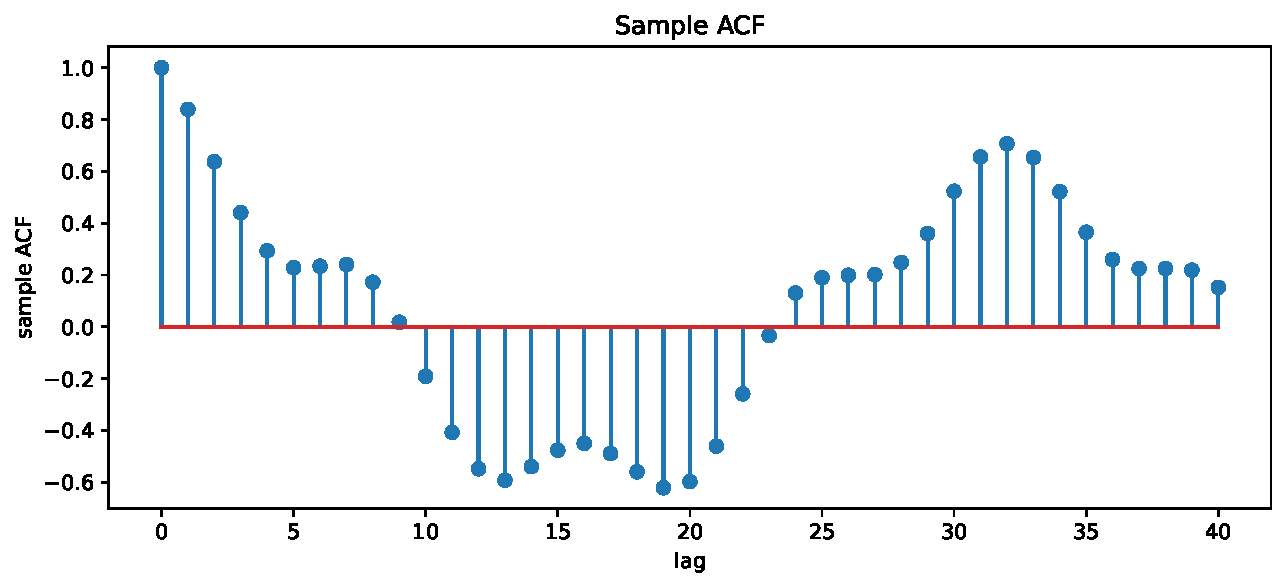
\includegraphics[keepaspectratio]{chapters/chapter-12-spectral-analysis-frequency-domain_files/figure-pdf/ch12-full-workflow-output-2.pdf}}

\pandocbounded{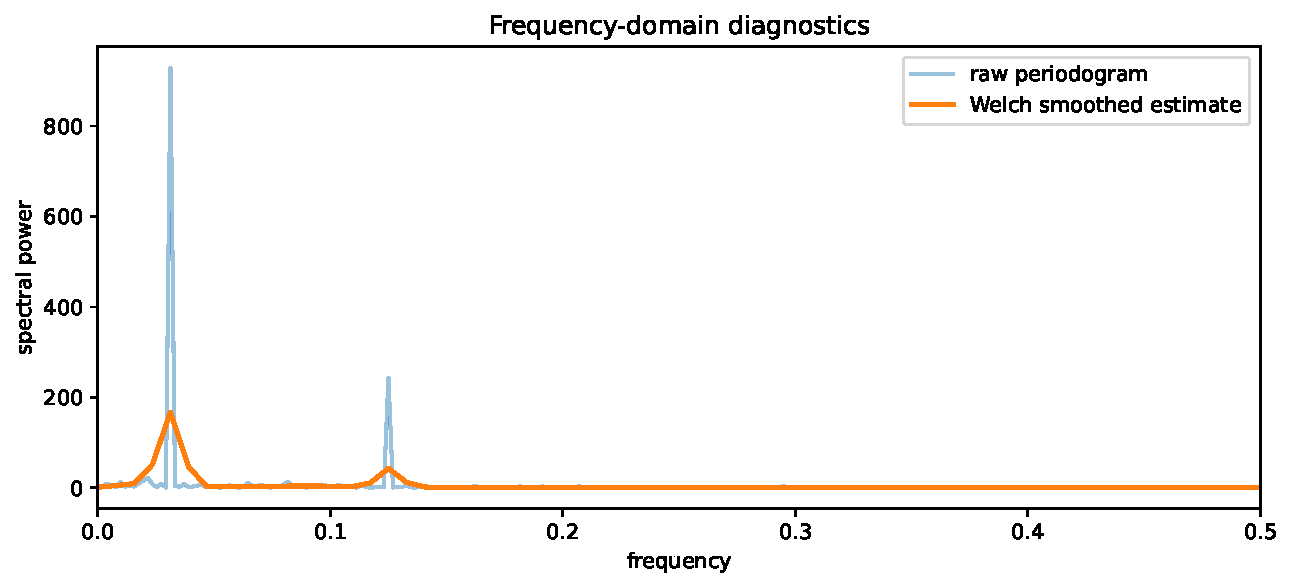
\includegraphics[keepaspectratio]{chapters/chapter-12-spectral-analysis-frequency-domain_files/figure-pdf/ch12-full-workflow-output-3.pdf}}

In this example, the true periods are \(32\) and \(8\). The
corresponding frequencies are \(1/32\) and \(1/8\). The spectral plot
should show elevated power near those frequencies, while the AR noise
adds low-frequency structure.

\section{12.17 Common mistakes}\label{common-mistakes-11}

\begin{enumerate}
\def\labelenumi{\arabic{enumi}.}
\tightlist
\item
  \textbf{Confusing period and frequency.} A frequency of \(0.05\) means
  a period of \(20\), not \(0.05\) time units.
\item
  \textbf{Ignoring the sampling rate.} A weekly cycle means different
  things for hourly, daily, and monthly data.
\item
  \textbf{Reading too much from a raw periodogram.} Raw periodograms are
  noisy. Use smoothing or repeated evidence.
\item
  \textbf{Applying spectral density theory to nonstationary data without
  caution.} Trend and changing variance can dominate the spectrum.
\item
  \textbf{Forgetting aliasing.} Frequencies outside the fundamental
  range are not separately identifiable from discrete observations.
\item
  \textbf{Treating a spectral peak as causal evidence.} A peak suggests
  periodic structure, not necessarily a scientific cause.
\item
  \textbf{Using random train-test splits after spectral feature
  extraction.} Frequency-domain features must be evaluated with
  time-aware validation.
\end{enumerate}

\section{12.18 Mini project: detect hidden
cycles}\label{mini-project-detect-hidden-cycles}

Choose or simulate a time series with at least one hidden periodic
component. Your report should include:

\begin{enumerate}
\def\labelenumi{\arabic{enumi}.}
\tightlist
\item
  a time plot;
\item
  an ACF plot;
\item
  a raw periodogram or smoothed spectral estimate;
\item
  a table translating the top spectral peaks into periods;
\item
  a proposed time-domain explanation;
\item
  one diagnostic that could refute your explanation;
\item
  a short AI-assisted critique paragraph, including what you accepted
  and what you rejected.
\end{enumerate}

A good project does not merely say ``there is a peak.'' It explains what
the peak means, why it may be real, and why it may be an artifact.

\section{12.19 Exercises}\label{exercises-11}

\begin{enumerate}
\def\labelenumi{\arabic{enumi}.}
\item
  \textbf{Frequency and period.} For each frequency
  \(\omega=1/4,1/7,1/12,1/24\), compute the period. Give one real-world
  example for each.
\item
  \textbf{Aliasing.} Show that for integer \(t\),

  \[
  \cos(2\pi\omega t)=\cos(2\pi(1-\omega)t).
  \]

  Explain why this matters for sampled data.
\item
  \textbf{Random sinusoid stationarity.} Let

  \[
  X_t=A\cos(2\pi\omega t)+B\sin(2\pi\omega t),
  \]

  where \(A\) and \(B\) are uncorrelated, mean zero, and have variance
  \(\sigma^2\). Prove that \(\{X_t\}\) is weakly stationary and compute
  \(\gamma(h)\).
\item
  \textbf{White noise spectrum.} Starting from the autocovariance of
  white noise, derive \(f(\omega)=\sigma^2\).
\item
  \textbf{AR(1) interpretation.} For \(\phi=0.8\) and \(\phi=-0.8\),
  determine whether the spectrum is larger near \(\omega=0\) or near
  \(\omega=1/2\). Explain the time-domain behavior.
\item
  \textbf{MA(1) derivation.} Derive the MA(1) spectral density

  \[
  f(\omega)=\sigma^2(1+\theta^2+2\theta\cos(2\pi\omega)).
  \]
\item
  \textbf{ARMA formula.} For an ARMA(1,1) model

  \[
  (1-\phi B)X_t=(1+\theta B)W_t,
  \]

  write its spectral density.
\item
  \textbf{Simulation.} Simulate an AR(1) process with \(\phi=0.9\) and
  another with \(\phi=-0.9\). Plot the time series and periodograms.
  Explain how the plots match the theory.
\item
  \textbf{Spectral peak.} A daily time series has a spectral peak at
  \(\omega=1/7\). What period does this correspond to? What diagnostic
  would help determine whether this is a genuine weekly cycle?
\item
  \textbf{AI critique.} Ask an AI assistant to interpret a periodogram
  from a simulated series with known frequencies. Identify one correct
  statement, one incomplete statement, and one statement that required
  mathematical verification.
\end{enumerate}

\section{12.20 Chapter checklist}\label{chapter-checklist-9}

By the end of this chapter, you should be able to:

\begin{itemize}
\tightlist
\item[$\square$]
  explain frequency-domain analysis in your own words;
\item[$\square$]
  convert between frequency and period;
\item[$\square$]
  explain aliasing and the Nyquist frequency;
\item[$\square$]
  derive the autocovariance of a random sinusoid;
\item[$\square$]
  define spectral distribution and spectral density;
\item[$\square$]
  state the Fourier-pair relationship between \(\gamma(h)\) and
  \(f(\omega)\);
\item[$\square$]
  interpret the integral of \(f(\omega)\) as variance;
\item[$\square$]
  derive spectra for white noise, AR(1), and MA(1);
\item[$\square$]
  write the spectral density of a causal ARMA model;
\item[$\square$]
  use Python to compute and interpret spectral diagnostics;
\item[$\square$]
  use AI assistance while checking stationarity, aliasing, and model
  assumptions.
\end{itemize}

\section{12.21 Further reading}\label{further-reading-2}

\begin{itemize}
\tightlist
\item
  Shumway and Stoffer, \emph{Time Series Analysis and Its Applications},
  chapters on spectral analysis.
\item
  Brockwell and Davis, \emph{Introduction to Time Series and
  Forecasting}, sections on spectral representation.
\item
  Percival and Walden, \emph{Spectral Analysis for Physical
  Applications}, for a deeper treatment of spectra and estimation.
\item
  Oppenheim and Schafer, \emph{Discrete-Time Signal Processing}, for the
  signal-processing viewpoint.
\end{itemize}

\chapter{Discrete Fourier Transform, FFT, and the
Periodogram}\label{discrete-fourier-transform-fft-and-the-periodogram}

\textbf{Part IV. Frequency-Domain and Multiresolution Methods}\\
\textbf{Chapter goal:} move from the population spectral density of
Chapter 12 to finite-sample spectral estimation. We develop the discrete
Fourier transform as a change of basis, the fast Fourier transform as an
efficient algorithm, the periodogram as a sample spectrum, and smoothed
periodograms as practical estimators of dominant frequencies.

\section{Learning objectives}\label{learning-objectives-12}

After studying this chapter, you should be able to:

\begin{enumerate}
\def\labelenumi{\arabic{enumi}.}
\tightlist
\item
  represent a finite time series as a vector in a complex Fourier basis;
\item
  define Fourier frequencies and explain why they are natural for data
  of length \(n\);
\item
  derive the discrete Fourier transform from orthogonal projection;
\item
  use Parseval's identity to connect time-domain energy and
  frequency-domain energy;
\item
  define the periodogram and interpret it as variance assigned to
  frequencies;
\item
  explain why the raw periodogram is noisy and why smoothing is needed;
\item
  compute DFTs and periodograms using direct formulas and the FFT;
\item
  recognize leakage, resolution limits, and aliasing in finite samples;
\item
  use the periodogram to propose periodic structure, then verify it by
  time-domain modeling;
\item
  use AI tools to help interpret spectral evidence while checking
  scaling, leakage, and sampling assumptions.
\end{enumerate}

\section{13.1 From population spectrum to sample
spectrum}\label{from-population-spectrum-to-sample-spectrum}

In Chapter 12 we studied the \textbf{spectral density} \(f(\omega)\) of
a stationary process. It is a population quantity satisfying

\[
\gamma(h)=\int_{-1/2}^{1/2} e^{2\pi i\omega h} f(\omega)\,d\omega,
\]

and, when \(\sum_h |\gamma(h)|<\infty\),

\[
f(\omega)=\sum_{h=-\infty}^{\infty}\gamma(h)e^{-2\pi i\omega h}.
\]

In practice, we do not observe the entire process. We observe one finite
realization

\[
x_0,x_1,\ldots,x_{n-1}.
\]

The main problem of this chapter is:

\begin{quote}
Given \(x_0,\ldots,x_{n-1}\), how can we estimate where the variance of
the series lives in frequency?
\end{quote}

There are two closely related answers.

First, estimate the autocovariance \(\gamma(h)\) by the sample
autocovariance \(\widehat{\gamma}(h)\) and plug it into the
Fourier-series formula for \(f(\omega)\).

Second, compute the discrete Fourier transform of the observed sequence
and square its magnitude. This gives the \textbf{periodogram}.

At the Fourier frequencies \(\omega_k=k/n\), these two approaches are
essentially the same, up to details of normalization and centering. The
periodogram is the computationally natural form because the fast Fourier
transform computes it extremely quickly.

\begin{tcolorbox}[enhanced jigsaw, arc=.35mm, bottomrule=.15mm, bottomtitle=1mm, breakable, colback=white, colbacktitle=quarto-callout-note-color!10!white, colframe=quarto-callout-note-color-frame, coltitle=black, left=2mm, leftrule=.75mm, opacityback=0, opacitybacktitle=0.6, rightrule=.15mm, title=\textcolor{quarto-callout-note-color}{\faInfo}\hspace{0.5em}{Population versus sample}, titlerule=0mm, toprule=.15mm, toptitle=1mm]

The spectral density \(f(\omega)\) is a property of the data-generating
process. The periodogram \(I(\omega_k)\) is computed from one finite
sample. It is a noisy finite-sample object, not the true spectrum
itself.

\end{tcolorbox}

\section{13.2 Fourier frequencies}\label{fourier-frequencies}

For a sample of length \(n\), the natural discrete frequencies are

\[
\omega_k=\frac{k}{n}, \qquad k=0,1,\ldots,n-1.
\]

The corresponding complex exponential sequence is

\[
e_k(t)=\exp(2\pi i\omega_k t)=\exp\left(2\pi i\frac{kt}{n}\right),
\qquad t=0,1,\ldots,n-1.
\]

These frequencies are natural because each sequence \(e_k(t)\) completes
exactly \(k\) cycles over a block of length \(n\). Also,

\[
e_k(t+n)=e_k(t),
\]

so these functions are periodic on the observed sample grid.

For real-valued time series, the positive and negative frequencies are
paired. Since

\[
\exp(2\pi i(1-\omega)t)=\exp(-2\pi i\omega t),
\]

the frequencies above \(1/2\) correspond to negative frequencies.
Therefore, one-sided periodogram plots usually show only

\[
0\leq \omega\leq \frac{1}{2}.
\]

The upper endpoint \(1/2\) is the Nyquist frequency.

\subsection{Period interpretation}\label{period-interpretation}

If a periodogram has a peak at \(\omega=0.05\), the corresponding period
is

\[
\frac{1}{0.05}=20
\]

time steps per cycle.

If the data are monthly and a peak occurs at \(\omega=1/12\), the period
is \(12\) months. If the data are daily and a peak occurs at
\(\omega=1/7\), the period is \(7\) days.

\section{13.3 The Fourier basis as an orthonormal
basis}\label{the-fourier-basis-as-an-orthonormal-basis}

Let \(\mathbb{C}^n\) be the vector space of complex-valued sequences of
length \(n\). Define the inner product

\[
\langle a,b\rangle=\sum_{t=0}^{n-1} a_t\overline{b_t}.
\]

For \(k=0,1,\ldots,n-1\), define

\[
\phi_k(t)=\frac{1}{\sqrt n}\exp\left(2\pi i\frac{kt}{n}\right).
\]

Then \(\{\phi_0,\phi_1,\ldots,\phi_{n-1}\}\) is an orthonormal basis of
\(\mathbb{C}^n\). Indeed,

\[
\langle \phi_j,\phi_k\rangle
=\frac{1}{n}\sum_{t=0}^{n-1}\exp\left(2\pi i\frac{(j-k)t}{n}\right).
\]

If \(j=k\), every term is \(1\), so the sum is \(1\). If \(j\neq k\),
this is a finite geometric series with ratio not equal to \(1\), and the
sum is \(0\).

Thus every finite sequence \(x=(x_0,\ldots,x_{n-1})\) has the expansion

\[
x=\sum_{k=0}^{n-1} c_k\phi_k,
\]

where

\[
c_k=\langle x,\phi_k\rangle
=\frac{1}{\sqrt n}\sum_{t=0}^{n-1}x_t\exp\left(-2\pi i\frac{kt}{n}\right).
\]

These coefficients \(c_k\) are the unitary discrete Fourier transform
coefficients.

\begin{tcolorbox}[enhanced jigsaw, arc=.35mm, bottomrule=.15mm, bottomtitle=1mm, breakable, colback=white, colbacktitle=quarto-callout-important-color!10!white, colframe=quarto-callout-important-color-frame, coltitle=black, left=2mm, leftrule=.75mm, opacityback=0, opacitybacktitle=0.6, rightrule=.15mm, title=\textcolor{quarto-callout-important-color}{\faExclamation}\hspace{0.5em}{DFT as coordinates}, titlerule=0mm, toprule=.15mm, toptitle=1mm]

The DFT is not mysterious. It is the coordinate vector of \(x\) in the
Fourier basis. It tells us how much of each sinusoidal basis direction
is present in the observed sequence.

\end{tcolorbox}

\section{13.4 DFT conventions and
scaling}\label{dft-conventions-and-scaling}

Different books and software packages use slightly different
normalizations. The mathematics is the same, but the scaling changes.

A common unnormalized DFT is

\[
D_k=\sum_{t=0}^{n-1}x_t\exp\left(-2\pi i\frac{kt}{n}\right).
\]

The inverse transform is

\[
x_t=\frac{1}{n}\sum_{k=0}^{n-1}D_k\exp\left(2\pi i\frac{kt}{n}\right).
\]

The unitary coefficient from the previous section is

\[
c_k=\frac{D_k}{\sqrt n}.
\]

Some time-series texts use the scaled coefficient

\[
X(\omega_k)=\frac{1}{n}D_k
=\frac{1}{n}\sum_{t=0}^{n-1}x_t\exp(-2\pi i\omega_k t).
\]

In this chapter, when we define the periodogram, we use

\[
I(\omega_k)=\frac{1}{n}|D_k|^2=|c_k|^2.
\]

With this convention, Parseval's identity becomes particularly simple:

\[
\sum_{t=0}^{n-1}|x_t|^2
=\sum_{k=0}^{n-1}I(\omega_k).
\]

If the data are centered, then

\[
\frac{1}{n}\sum_{t=0}^{n-1}(x_t-\bar x)^2
=\frac{1}{n}\sum_{k=0}^{n-1}I(\omega_k).
\]

Thus the periodogram divides the sample energy, or variance after
centering, across Fourier frequencies.

\subsection{Python: direct DFT versus NumPy
FFT}\label{python-direct-dft-versus-numpy-fft}

\begin{Shaded}
\begin{Highlighting}[]
\ImportTok{import}\NormalTok{ numpy }\ImportTok{as}\NormalTok{ np}
\ImportTok{import}\NormalTok{ matplotlib.pyplot }\ImportTok{as}\NormalTok{ plt}

\NormalTok{rng }\OperatorTok{=}\NormalTok{ np.random.default\_rng(}\DecValTok{7339}\NormalTok{)}
\NormalTok{n }\OperatorTok{=} \DecValTok{32}
\NormalTok{t }\OperatorTok{=}\NormalTok{ np.arange(n)}
\NormalTok{x }\OperatorTok{=} \FloatTok{1.2} \OperatorTok{*}\NormalTok{ np.cos(}\DecValTok{2} \OperatorTok{*}\NormalTok{ np.pi }\OperatorTok{*} \DecValTok{4} \OperatorTok{*}\NormalTok{ t }\OperatorTok{/}\NormalTok{ n) }\OperatorTok{+} \FloatTok{0.5} \OperatorTok{*}\NormalTok{ rng.normal(size}\OperatorTok{=}\NormalTok{n)}
\NormalTok{x }\OperatorTok{=}\NormalTok{ x }\OperatorTok{{-}}\NormalTok{ x.mean()}

\CommentTok{\# Direct DFT matrix: D\_k = sum\_t x\_t exp({-}2 pi i k t / n)}
\NormalTok{k }\OperatorTok{=}\NormalTok{ np.arange(n)}
\NormalTok{W }\OperatorTok{=}\NormalTok{ np.exp(}\OperatorTok{{-}}\OtherTok{2j} \OperatorTok{*}\NormalTok{ np.pi }\OperatorTok{*}\NormalTok{ np.outer(k, t) }\OperatorTok{/}\NormalTok{ n)}
\NormalTok{D\_direct }\OperatorTok{=}\NormalTok{ W }\OperatorTok{@}\NormalTok{ x}

\CommentTok{\# NumPy FFT uses the same unnormalized convention.}
\NormalTok{D\_fft }\OperatorTok{=}\NormalTok{ np.fft.fft(x)}

\BuiltInTok{print}\NormalTok{(}\StringTok{"maximum absolute difference:"}\NormalTok{, np.}\BuiltInTok{max}\NormalTok{(np.}\BuiltInTok{abs}\NormalTok{(D\_direct }\OperatorTok{{-}}\NormalTok{ D\_fft)))}

\NormalTok{freq }\OperatorTok{=}\NormalTok{ np.fft.fftfreq(n, d}\OperatorTok{=}\DecValTok{1}\NormalTok{)}
\NormalTok{periodogram }\OperatorTok{=}\NormalTok{ (np.}\BuiltInTok{abs}\NormalTok{(D\_fft) }\OperatorTok{**} \DecValTok{2}\NormalTok{) }\OperatorTok{/}\NormalTok{ n}

\NormalTok{plt.figure(figsize}\OperatorTok{=}\NormalTok{(}\DecValTok{9}\NormalTok{, }\DecValTok{4}\NormalTok{))}
\NormalTok{plt.stem(freq[: n }\OperatorTok{//} \DecValTok{2} \OperatorTok{+} \DecValTok{1}\NormalTok{], periodogram[: n }\OperatorTok{//} \DecValTok{2} \OperatorTok{+} \DecValTok{1}\NormalTok{])}
\NormalTok{plt.xlabel(}\StringTok{"frequency"}\NormalTok{)}
\NormalTok{plt.ylabel(}\StringTok{"periodogram"}\NormalTok{)}
\NormalTok{plt.title(}\StringTok{"One{-}sided periodogram from the FFT"}\NormalTok{)}
\NormalTok{plt.show()}
\end{Highlighting}
\end{Shaded}

\begin{verbatim}
maximum absolute difference: 6.898122193969271e-14
\end{verbatim}

\begin{figure}[H]

{\centering \pandocbounded{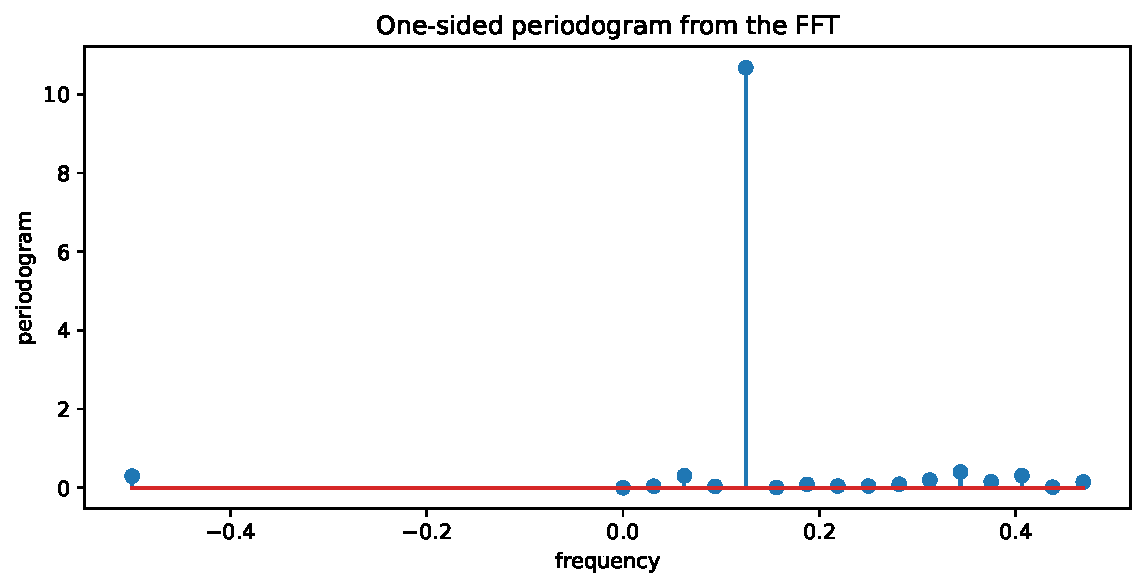
\includegraphics[keepaspectratio]{chapters/chapter-13-dft-fft-periodogram_files/figure-pdf/ch13-direct-dft-vs-fft-output-2.pdf}}

}

\caption{Direct DFT and FFT give the same coefficients up to numerical
precision.}

\end{figure}%

\section{13.5 The periodogram}\label{the-periodogram}

The \textbf{periodogram} at Fourier frequency \(\omega_k=k/n\) is

\[
I(\omega_k)=\frac{1}{n}\left|\sum_{t=0}^{n-1}x_t e^{-2\pi i\omega_k t}\right|^2.
\]

Equivalently, writing the real and imaginary components,

\[
\sum_{t=0}^{n-1}x_t e^{-2\pi i\omega_k t}
=\sum_{t=0}^{n-1}x_t\cos(2\pi\omega_k t)
-i\sum_{t=0}^{n-1}x_t\sin(2\pi\omega_k t).
\]

Therefore,

\[
I(\omega_k)
=\frac{1}{n}\left(\sum_{t=0}^{n-1}x_t\cos(2\pi\omega_k t)\right)^2
+\frac{1}{n}\left(\sum_{t=0}^{n-1}x_t\sin(2\pi\omega_k t)\right)^2.
\]

This formula shows the regression interpretation: the periodogram is
large at a frequency if the data have a strong projection onto the sine
and cosine waves at that frequency.

\subsection{Centering and the zero
frequency}\label{centering-and-the-zero-frequency}

The frequency \(\omega_0=0\) corresponds to the constant basis vector.
Since

\[
D_0=\sum_{t=0}^{n-1}x_t=n\bar x,
\]

the zero-frequency periodogram is

\[
I(0)=n\bar x^2.
\]

If the mean is not removed, the zero-frequency spike may dominate the
plot. For spectral analysis of fluctuations around a mean, we usually
center the data first.

\begin{tcolorbox}[enhanced jigsaw, arc=.35mm, bottomrule=.15mm, bottomtitle=1mm, breakable, colback=white, colbacktitle=quarto-callout-warning-color!10!white, colframe=quarto-callout-warning-color-frame, coltitle=black, left=2mm, leftrule=.75mm, opacityback=0, opacitybacktitle=0.6, rightrule=.15mm, title=\textcolor{quarto-callout-warning-color}{\faExclamationTriangle}\hspace{0.5em}{Center before interpreting peaks}, titlerule=0mm, toprule=.15mm, toptitle=1mm]

A strong mean or trend can create large low-frequency power. Before
interpreting the periodogram, ask whether you should center, detrend,
difference, or otherwise remove deterministic structure.

\end{tcolorbox}

\subsection{Python: periodogram of a hidden periodic
signal}\label{python-periodogram-of-a-hidden-periodic-signal}

\protect\phantomsection\label{ch13-periodogram-hidden-cycle}
\begin{Shaded}
\begin{Highlighting}[]
\NormalTok{rng }\OperatorTok{=}\NormalTok{ np.random.default\_rng(}\DecValTok{2026}\NormalTok{)}
\NormalTok{n }\OperatorTok{=} \DecValTok{240}
\NormalTok{t }\OperatorTok{=}\NormalTok{ np.arange(n)}
\NormalTok{true\_period }\OperatorTok{=} \DecValTok{30}
\NormalTok{true\_freq }\OperatorTok{=} \DecValTok{1} \OperatorTok{/}\NormalTok{ true\_period}

\NormalTok{x }\OperatorTok{=} \FloatTok{1.5} \OperatorTok{*}\NormalTok{ np.cos(}\DecValTok{2} \OperatorTok{*}\NormalTok{ np.pi }\OperatorTok{*}\NormalTok{ true\_freq }\OperatorTok{*}\NormalTok{ t }\OperatorTok{+} \FloatTok{0.6}\NormalTok{) }\OperatorTok{+} \FloatTok{0.8} \OperatorTok{*}\NormalTok{ rng.normal(size}\OperatorTok{=}\NormalTok{n)}
\NormalTok{x\_centered }\OperatorTok{=}\NormalTok{ x }\OperatorTok{{-}}\NormalTok{ x.mean()}

\NormalTok{D }\OperatorTok{=}\NormalTok{ np.fft.rfft(x\_centered)}
\NormalTok{freq }\OperatorTok{=}\NormalTok{ np.fft.rfftfreq(n, d}\OperatorTok{=}\DecValTok{1}\NormalTok{)}
\NormalTok{I }\OperatorTok{=}\NormalTok{ np.}\BuiltInTok{abs}\NormalTok{(D) }\OperatorTok{**} \DecValTok{2} \OperatorTok{/}\NormalTok{ n}

\CommentTok{\# Ignore frequency zero when searching for a periodic peak.}
\NormalTok{peak\_idx }\OperatorTok{=} \DecValTok{1} \OperatorTok{+}\NormalTok{ np.argmax(I[}\DecValTok{1}\NormalTok{:])}
\NormalTok{peak\_freq }\OperatorTok{=}\NormalTok{ freq[peak\_idx]}
\NormalTok{peak\_period }\OperatorTok{=} \DecValTok{1} \OperatorTok{/}\NormalTok{ peak\_freq}

\BuiltInTok{print}\NormalTok{(}\StringTok{"True period:"}\NormalTok{, true\_period)}
\BuiltInTok{print}\NormalTok{(}\StringTok{"Estimated peak frequency:"}\NormalTok{, }\BuiltInTok{round}\NormalTok{(peak\_freq, }\DecValTok{4}\NormalTok{))}
\BuiltInTok{print}\NormalTok{(}\StringTok{"Estimated peak period:"}\NormalTok{, }\BuiltInTok{round}\NormalTok{(peak\_period, }\DecValTok{2}\NormalTok{))}

\NormalTok{plt.figure(figsize}\OperatorTok{=}\NormalTok{(}\DecValTok{10}\NormalTok{, }\DecValTok{4}\NormalTok{))}
\NormalTok{plt.plot(t, x)}
\NormalTok{plt.xlabel(}\StringTok{"time"}\NormalTok{)}
\NormalTok{plt.ylabel(}\StringTok{"value"}\NormalTok{)}
\NormalTok{plt.title(}\StringTok{"Noisy periodic signal"}\NormalTok{)}
\NormalTok{plt.show()}

\NormalTok{plt.figure(figsize}\OperatorTok{=}\NormalTok{(}\DecValTok{10}\NormalTok{, }\DecValTok{4}\NormalTok{))}
\NormalTok{plt.plot(freq[}\DecValTok{1}\NormalTok{:], I[}\DecValTok{1}\NormalTok{:])}
\NormalTok{plt.axvline(true\_freq, linestyle}\OperatorTok{=}\StringTok{"{-}{-}"}\NormalTok{, label}\OperatorTok{=}\StringTok{"true frequency"}\NormalTok{)}
\NormalTok{plt.axvline(peak\_freq, linestyle}\OperatorTok{=}\StringTok{":"}\NormalTok{, label}\OperatorTok{=}\StringTok{"largest periodogram peak"}\NormalTok{)}
\NormalTok{plt.xlabel(}\StringTok{"frequency"}\NormalTok{)}
\NormalTok{plt.ylabel(}\StringTok{"periodogram"}\NormalTok{)}
\NormalTok{plt.title(}\StringTok{"Periodogram"}\NormalTok{)}
\NormalTok{plt.legend()}
\NormalTok{plt.show()}
\end{Highlighting}
\end{Shaded}

\begin{verbatim}
True period: 30
Estimated peak frequency: 0.0333
Estimated peak period: 30.0
\end{verbatim}

\begin{figure}[H]

{\centering \pandocbounded{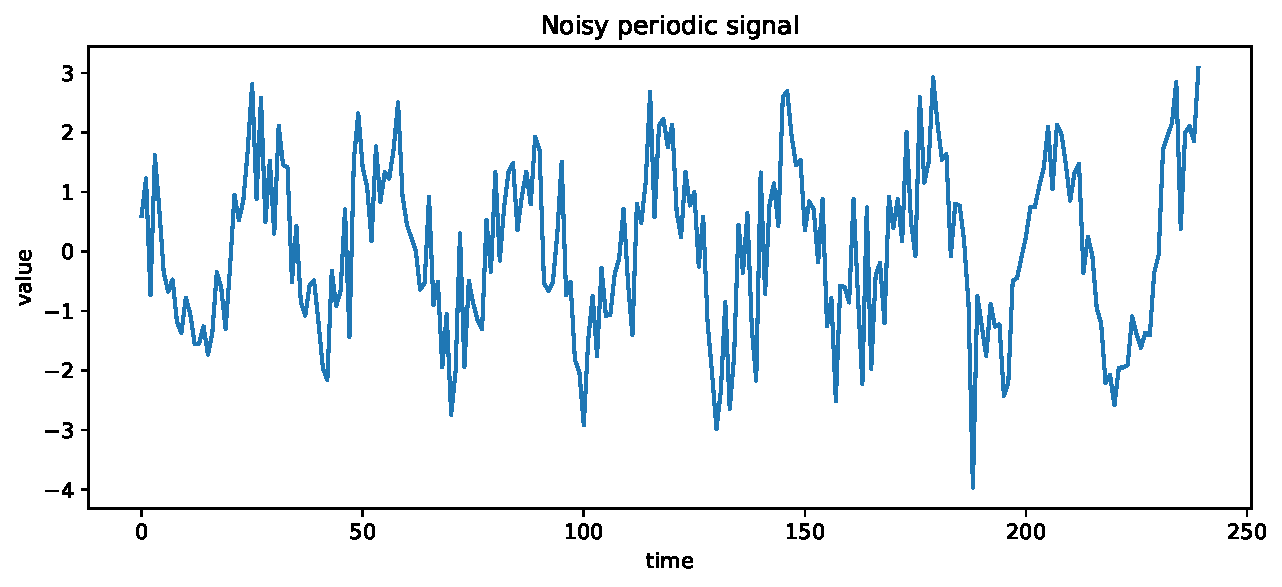
\includegraphics[keepaspectratio]{chapters/chapter-13-dft-fft-periodogram_files/figure-pdf/ch13-periodogram-hidden-cycle-output-2.pdf}}

}

\caption{The periodogram reveals the hidden frequency of a noisy
sinusoidal signal.}

\end{figure}%

\pandocbounded{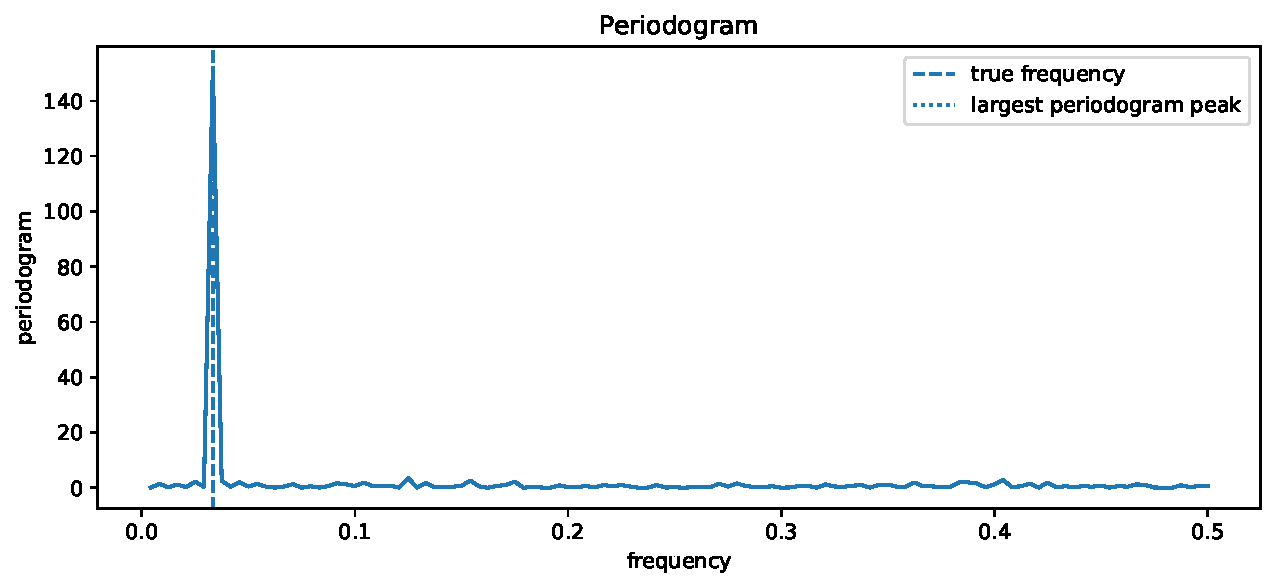
\includegraphics[keepaspectratio]{chapters/chapter-13-dft-fft-periodogram_files/figure-pdf/ch13-periodogram-hidden-cycle-output-3.pdf}}

\section{13.6 The periodogram and sample
autocovariance}\label{the-periodogram-and-sample-autocovariance}

For centered data, define a circular sample autocovariance

\[
\widetilde{\gamma}(h)=\frac{1}{n}\sum_{t=0}^{n-1}x_t x_{t+h \;\mathrm{mod}\; n}.
\]

Then the periodogram can be written as the discrete Fourier transform of
\(\widetilde{\gamma}(h)\):

\[
I(\omega_k)=\sum_{h=0}^{n-1}\widetilde{\gamma}(h)e^{-2\pi i\omega_k h}.
\]

This is the finite-sample analog of

\[
f(\omega)=\sum_{h=-\infty}^{\infty}\gamma(h)e^{-2\pi i\omega h}.
\]

The usual non-circular sample autocovariance is

\[
\widehat{\gamma}(h)=\frac{1}{n}\sum_{t=0}^{n-1-h}(x_{t+h}-\bar x)(x_t-\bar x),
\qquad h\geq 0.
\]

Using \(\widehat{\gamma}(h)\) in a finite Fourier sum gives another form
of spectral estimate. At Fourier frequencies, the periodogram is the
most common computational object.

\section{13.7 Why the raw periodogram is
noisy}\label{why-the-raw-periodogram-is-noisy}

The periodogram is asymptotically unbiased under suitable regularity
conditions, but it is not a consistent estimator of \(f(\omega)\)
without smoothing. Informally:

\begin{itemize}
\tightlist
\item
  as \(n\) grows, the frequency grid becomes denser;
\item
  the expected periodogram approaches the true spectrum;
\item
  but the variance of the periodogram at a fixed frequency does not
  vanish.
\end{itemize}

This means the raw periodogram remains jagged even for long series. It
is useful for detecting strong peaks, but it is usually too variable for
estimating a smooth spectral density.

A common remedy is to average nearby periodogram values:

\[
\widehat f(\omega_k)=\sum_{j=-m}^{m} a_j I(\omega_{k+j}),
\]

where \(a_j\geq 0\) and \(\sum_{j=-m}^{m}a_j=1\).

The window width controls a bias-variance tradeoff:

\begin{itemize}
\tightlist
\item
  more smoothing decreases variance but blurs narrow peaks;
\item
  less smoothing preserves sharp peaks but leaves high variance.
\end{itemize}

\subsection{Python: smoothing a
periodogram}\label{python-smoothing-a-periodogram}

\begin{Shaded}
\begin{Highlighting}[]
\NormalTok{rng }\OperatorTok{=}\NormalTok{ np.random.default\_rng(}\DecValTok{1}\NormalTok{)}
\NormalTok{n }\OperatorTok{=} \DecValTok{512}
\NormalTok{t }\OperatorTok{=}\NormalTok{ np.arange(n)}

\CommentTok{\# AR(1){-}like smooth process plus a periodic component.}
\NormalTok{phi }\OperatorTok{=} \FloatTok{0.85}
\NormalTok{w }\OperatorTok{=}\NormalTok{ rng.normal(size}\OperatorTok{=}\NormalTok{n)}
\NormalTok{y }\OperatorTok{=}\NormalTok{ np.zeros(n)}
\ControlFlowTok{for}\NormalTok{ i }\KeywordTok{in} \BuiltInTok{range}\NormalTok{(}\DecValTok{1}\NormalTok{, n):}
\NormalTok{    y[i] }\OperatorTok{=}\NormalTok{ phi }\OperatorTok{*}\NormalTok{ y[i}\OperatorTok{{-}}\DecValTok{1}\NormalTok{] }\OperatorTok{+}\NormalTok{ w[i]}

\NormalTok{x }\OperatorTok{=}\NormalTok{ y }\OperatorTok{+} \FloatTok{1.5} \OperatorTok{*}\NormalTok{ np.cos(}\DecValTok{2} \OperatorTok{*}\NormalTok{ np.pi }\OperatorTok{*}\NormalTok{ (}\DecValTok{1}\OperatorTok{/}\DecValTok{40}\NormalTok{) }\OperatorTok{*}\NormalTok{ t)}
\NormalTok{x }\OperatorTok{=}\NormalTok{ x }\OperatorTok{{-}}\NormalTok{ x.mean()}

\NormalTok{freq }\OperatorTok{=}\NormalTok{ np.fft.rfftfreq(n, d}\OperatorTok{=}\DecValTok{1}\NormalTok{)}
\NormalTok{I }\OperatorTok{=}\NormalTok{ np.}\BuiltInTok{abs}\NormalTok{(np.fft.rfft(x)) }\OperatorTok{**} \DecValTok{2} \OperatorTok{/}\NormalTok{ n}

\CommentTok{\# Simple moving{-}average smoother over frequencies.}
\NormalTok{width }\OperatorTok{=} \DecValTok{9}
\NormalTok{kernel }\OperatorTok{=}\NormalTok{ np.ones(width) }\OperatorTok{/}\NormalTok{ width}
\NormalTok{I\_smooth }\OperatorTok{=}\NormalTok{ np.convolve(I, kernel, mode}\OperatorTok{=}\StringTok{"same"}\NormalTok{)}

\NormalTok{plt.figure(figsize}\OperatorTok{=}\NormalTok{(}\DecValTok{10}\NormalTok{, }\DecValTok{4}\NormalTok{))}
\NormalTok{plt.plot(freq[}\DecValTok{1}\NormalTok{:], I[}\DecValTok{1}\NormalTok{:], alpha}\OperatorTok{=}\FloatTok{0.5}\NormalTok{, label}\OperatorTok{=}\StringTok{"raw periodogram"}\NormalTok{)}
\NormalTok{plt.plot(freq[}\DecValTok{1}\NormalTok{:], I\_smooth[}\DecValTok{1}\NormalTok{:], linewidth}\OperatorTok{=}\DecValTok{2}\NormalTok{, label}\OperatorTok{=}\StringTok{"smoothed periodogram"}\NormalTok{)}
\NormalTok{plt.xlabel(}\StringTok{"frequency"}\NormalTok{)}
\NormalTok{plt.ylabel(}\StringTok{"spectral power"}\NormalTok{)}
\NormalTok{plt.title(}\StringTok{"Raw versus smoothed periodogram"}\NormalTok{)}
\NormalTok{plt.legend()}
\NormalTok{plt.show()}
\end{Highlighting}
\end{Shaded}

\begin{figure}[H]

{\centering \pandocbounded{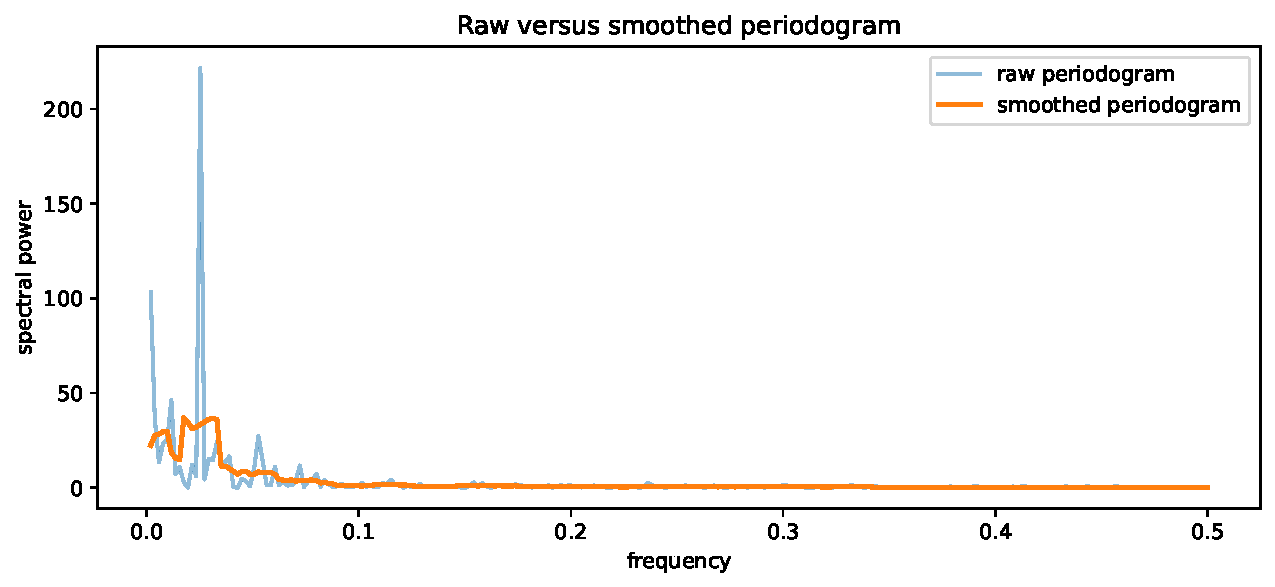
\includegraphics[keepaspectratio]{chapters/chapter-13-dft-fft-periodogram_files/figure-pdf/ch13-smoothed-periodogram-output-1.pdf}}

}

\caption{A smoothed periodogram reduces variance but blurs sharp
spectral features.}

\end{figure}%

\section{13.8 The fast Fourier
transform}\label{the-fast-fourier-transform}

The direct DFT formula requires computing

\[
D_k=\sum_{t=0}^{n-1}x_t e^{-2\pi i kt/n}
\]

for \(k=0,1,\ldots,n-1\). This involves about \(n^2\) complex
multiplications. For large \(n\), this is expensive.

The \textbf{fast Fourier transform} is an algorithm that computes the
same DFT coefficients in approximately

\[
O(n\log n)
\]

operations.

The key idea is to exploit symmetry. When \(n\) is even, split the DFT
into even and odd time indices:

\[
D_k
=\sum_{t=0}^{n-1}x_t e^{-2\pi i kt/n}
=\sum_{m=0}^{n/2-1}x_{2m} e^{-2\pi i k(2m)/n}
+\sum_{m=0}^{n/2-1}x_{2m+1} e^{-2\pi i k(2m+1)/n}.
\]

This becomes

\[
D_k
=\sum_{m=0}^{n/2-1}x_{2m} e^{-2\pi i km/(n/2)}
+e^{-2\pi i k/n}\sum_{m=0}^{n/2-1}x_{2m+1} e^{-2\pi i km/(n/2)}.
\]

The two sums are DFTs of length \(n/2\). Thus a DFT of length \(n\) can
be computed using two DFTs of length \(n/2\) plus a small amount of
recombination. Repeating the split gives the FFT.

\begin{tcolorbox}[enhanced jigsaw, arc=.35mm, bottomrule=.15mm, bottomtitle=1mm, breakable, colback=white, colbacktitle=quarto-callout-note-color!10!white, colframe=quarto-callout-note-color-frame, coltitle=black, left=2mm, leftrule=.75mm, opacityback=0, opacitybacktitle=0.6, rightrule=.15mm, title=\textcolor{quarto-callout-note-color}{\faInfo}\hspace{0.5em}{Algorithm, not a new transform}, titlerule=0mm, toprule=.15mm, toptitle=1mm]

The FFT does not define a new mathematical transform. It is a fast
algorithm for computing the DFT.

\end{tcolorbox}

\subsection{Python: timing direct DFT and
FFT}\label{python-timing-direct-dft-and-fft}

\protect\phantomsection\label{ch13-fft-speed}
\begin{Shaded}
\begin{Highlighting}[]
\ImportTok{import}\NormalTok{ time}

\NormalTok{rng }\OperatorTok{=}\NormalTok{ np.random.default\_rng(}\DecValTok{42}\NormalTok{)}

\ControlFlowTok{for}\NormalTok{ n }\KeywordTok{in}\NormalTok{ [}\DecValTok{128}\NormalTok{, }\DecValTok{256}\NormalTok{, }\DecValTok{512}\NormalTok{]:}
\NormalTok{    x }\OperatorTok{=}\NormalTok{ rng.normal(size}\OperatorTok{=}\NormalTok{n)}
\NormalTok{    t }\OperatorTok{=}\NormalTok{ np.arange(n)}
\NormalTok{    k }\OperatorTok{=}\NormalTok{ np.arange(n)}

\NormalTok{    start }\OperatorTok{=}\NormalTok{ time.perf\_counter()}
\NormalTok{    W }\OperatorTok{=}\NormalTok{ np.exp(}\OperatorTok{{-}}\OtherTok{2j} \OperatorTok{*}\NormalTok{ np.pi }\OperatorTok{*}\NormalTok{ np.outer(k, t) }\OperatorTok{/}\NormalTok{ n)}
\NormalTok{    D\_direct }\OperatorTok{=}\NormalTok{ W }\OperatorTok{@}\NormalTok{ x}
\NormalTok{    direct\_time }\OperatorTok{=}\NormalTok{ time.perf\_counter() }\OperatorTok{{-}}\NormalTok{ start}

\NormalTok{    start }\OperatorTok{=}\NormalTok{ time.perf\_counter()}
\NormalTok{    D\_fft }\OperatorTok{=}\NormalTok{ np.fft.fft(x)}
\NormalTok{    fft\_time }\OperatorTok{=}\NormalTok{ time.perf\_counter() }\OperatorTok{{-}}\NormalTok{ start}

\NormalTok{    error }\OperatorTok{=}\NormalTok{ np.}\BuiltInTok{max}\NormalTok{(np.}\BuiltInTok{abs}\NormalTok{(D\_direct }\OperatorTok{{-}}\NormalTok{ D\_fft))}
    \BuiltInTok{print}\NormalTok{(}\SpecialStringTok{f"n=}\SpecialCharTok{\{}\NormalTok{n}\SpecialCharTok{:4d\}}\SpecialStringTok{  direct=}\SpecialCharTok{\{}\NormalTok{direct\_time}\SpecialCharTok{:.4f\}}\SpecialStringTok{s  fft=}\SpecialCharTok{\{}\NormalTok{fft\_time}\SpecialCharTok{:.6f\}}\SpecialStringTok{s  error=}\SpecialCharTok{\{}\NormalTok{error}\SpecialCharTok{:.2e\}}\SpecialStringTok{"}\NormalTok{)}
\end{Highlighting}
\end{Shaded}

\begin{verbatim}
n= 128  direct=0.0032s  fft=0.000020s  error=4.71e-13
n= 256  direct=0.0054s  fft=0.000033s  error=1.88e-12
n= 512  direct=0.0119s  fft=0.000024s  error=5.72e-12
\end{verbatim}

\section{13.9 Spectral leakage and finite-sample
resolution}\label{spectral-leakage-and-finite-sample-resolution}

The Fourier basis frequencies are exactly \(k/n\). What happens if the
true signal has frequency not exactly equal to one of these grid
frequencies?

Suppose

\[
x_t=A\cos(2\pi\omega_0 t)
\]

where \(\omega_0\) is not equal to \(k/n\) for any integer \(k\). Then
the energy cannot be placed into one Fourier bin. It spreads into
neighboring bins. This is called \textbf{spectral leakage}.

Leakage is caused by observing a finite window of a signal.
Mathematically, truncating a signal in time corresponds to spreading its
spectrum in frequency.

A common practical remedy is to multiply the data by a taper or window
before applying the DFT. For example, a Hann taper is

\[
w_t=\frac{1}{2}\left(1-\cos\left(\frac{2\pi t}{n-1}\right)\right).
\]

Then we analyze \(w_t x_t\) rather than \(x_t\) directly. Tapering
reduces edge discontinuities, which often reduces leakage far away from
the main peak, but it also widens the main lobe.

\subsection{Python: leakage and
tapering}\label{python-leakage-and-tapering}

\begin{Shaded}
\begin{Highlighting}[]
\NormalTok{n }\OperatorTok{=} \DecValTok{128}
\NormalTok{t }\OperatorTok{=}\NormalTok{ np.arange(n)}

\CommentTok{\# Not an integer number of cycles over the sample.}
\NormalTok{cycles }\OperatorTok{=} \FloatTok{10.5}
\NormalTok{omega0 }\OperatorTok{=}\NormalTok{ cycles }\OperatorTok{/}\NormalTok{ n}
\NormalTok{x }\OperatorTok{=}\NormalTok{ np.cos(}\DecValTok{2} \OperatorTok{*}\NormalTok{ np.pi }\OperatorTok{*}\NormalTok{ omega0 }\OperatorTok{*}\NormalTok{ t)}
\NormalTok{x }\OperatorTok{=}\NormalTok{ x }\OperatorTok{{-}}\NormalTok{ x.mean()}

\NormalTok{hann }\OperatorTok{=} \FloatTok{0.5} \OperatorTok{*}\NormalTok{ (}\DecValTok{1} \OperatorTok{{-}}\NormalTok{ np.cos(}\DecValTok{2} \OperatorTok{*}\NormalTok{ np.pi }\OperatorTok{*}\NormalTok{ t }\OperatorTok{/}\NormalTok{ (n }\OperatorTok{{-}} \DecValTok{1}\NormalTok{)))}
\NormalTok{x\_hann }\OperatorTok{=}\NormalTok{ hann }\OperatorTok{*}\NormalTok{ x}

\NormalTok{freq }\OperatorTok{=}\NormalTok{ np.fft.rfftfreq(n, d}\OperatorTok{=}\DecValTok{1}\NormalTok{)}
\NormalTok{I\_raw }\OperatorTok{=}\NormalTok{ np.}\BuiltInTok{abs}\NormalTok{(np.fft.rfft(x)) }\OperatorTok{**} \DecValTok{2} \OperatorTok{/}\NormalTok{ n}
\NormalTok{I\_hann }\OperatorTok{=}\NormalTok{ np.}\BuiltInTok{abs}\NormalTok{(np.fft.rfft(x\_hann)) }\OperatorTok{**} \DecValTok{2} \OperatorTok{/}\NormalTok{ n}

\NormalTok{plt.figure(figsize}\OperatorTok{=}\NormalTok{(}\DecValTok{10}\NormalTok{, }\DecValTok{4}\NormalTok{))}
\NormalTok{plt.plot(freq, I\_raw }\OperatorTok{/}\NormalTok{ I\_raw.}\BuiltInTok{max}\NormalTok{(), label}\OperatorTok{=}\StringTok{"raw, normalized"}\NormalTok{)}
\NormalTok{plt.plot(freq, I\_hann }\OperatorTok{/}\NormalTok{ I\_hann.}\BuiltInTok{max}\NormalTok{(), label}\OperatorTok{=}\StringTok{"Hann tapered, normalized"}\NormalTok{)}
\NormalTok{plt.axvline(omega0, linestyle}\OperatorTok{=}\StringTok{"{-}{-}"}\NormalTok{, label}\OperatorTok{=}\StringTok{"true frequency"}\NormalTok{)}
\NormalTok{plt.xlim(}\DecValTok{0}\NormalTok{, }\FloatTok{0.18}\NormalTok{)}
\NormalTok{plt.xlabel(}\StringTok{"frequency"}\NormalTok{)}
\NormalTok{plt.ylabel(}\StringTok{"normalized periodogram"}\NormalTok{)}
\NormalTok{plt.title(}\StringTok{"Spectral leakage and tapering"}\NormalTok{)}
\NormalTok{plt.legend()}
\NormalTok{plt.show()}
\end{Highlighting}
\end{Shaded}

\begin{figure}[H]

{\centering \pandocbounded{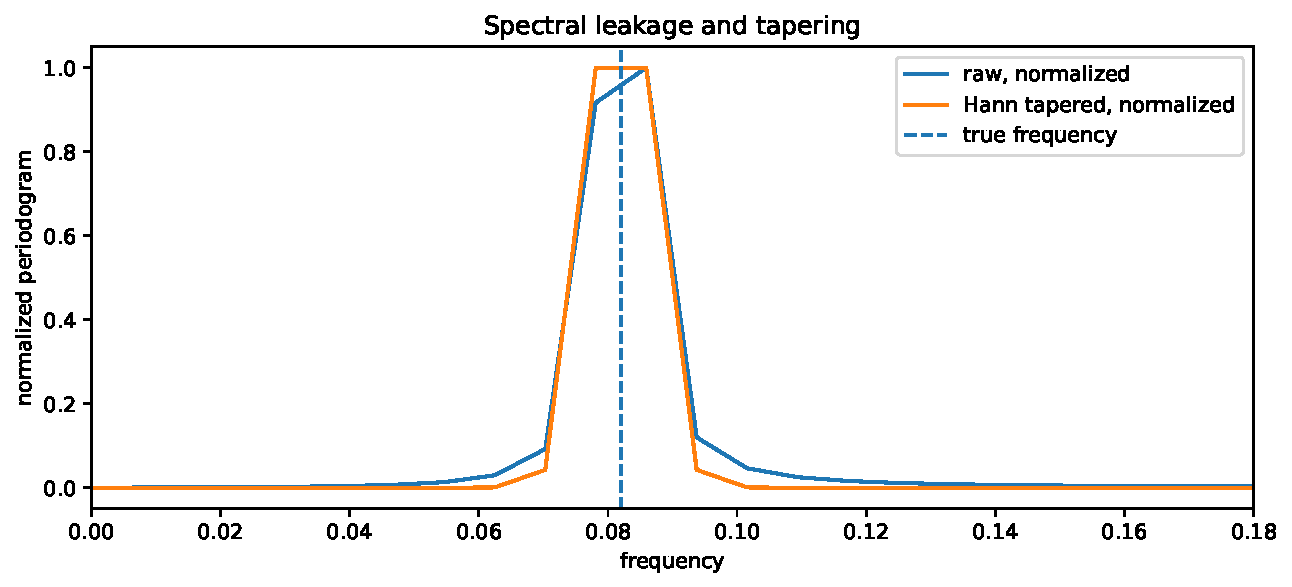
\includegraphics[keepaspectratio]{chapters/chapter-13-dft-fft-periodogram_files/figure-pdf/ch13-leakage-windowing-output-1.pdf}}

}

\caption{A frequency not aligned with the Fourier grid leaks energy into
nearby bins; tapering changes the leakage pattern.}

\end{figure}%

\section{13.10 Interactive HTML: DFT and periodogram
explorer}\label{interactive-html-dft-and-periodogram-explorer}

This interactive example lets you combine two sinusoids and noise, then
view the time series and its one-sided periodogram. It uses the global
Plotly.js import from the book header.

\section{DFT and periodogram
explorer}\label{dft-and-periodogram-explorer}

Adjust the two frequencies, amplitudes, and noise level. Frequencies are
measured in cycles per time step. The periodogram should peak near the
frequencies used to generate the signal, but finite-sample effects and
noise can make the picture imperfect.

Sample size n \protect\phantomsection\label{ch13-n-val}{160} Frequency 1
\protect\phantomsection\label{ch13-f1-val}{0.08} Amplitude 1
\protect\phantomsection\label{ch13-a1-val}{2.0} Frequency 2
\protect\phantomsection\label{ch13-f2-val}{0.21} Amplitude 2
\protect\phantomsection\label{ch13-a2-val}{1.0} Noise level
\protect\phantomsection\label{ch13-noise-val}{0.6}

\protect\phantomsection\label{ch13-time-plot}

\protect\phantomsection\label{ch13-periodogram-plot}

\section{13.11 Detecting a period is not the same as proving a
model}\label{detecting-a-period-is-not-the-same-as-proving-a-model}

The periodogram is a powerful exploratory tool. A large peak suggests
that a sinusoidal component may be present. But a peak alone is not a
complete model.

A responsible workflow is:

\begin{enumerate}
\def\labelenumi{\arabic{enumi}.}
\tightlist
\item
  center, detrend, or difference if necessary;
\item
  inspect the periodogram;
\item
  identify candidate frequencies;
\item
  translate frequencies into periods;
\item
  fit a time-domain model using sine and cosine regressors;
\item
  inspect residuals using time plots, ACF, and diagnostics;
\item
  compare with baseline forecasts.
\end{enumerate}

\subsection{Python: peak detection followed by sinusoidal
regression}\label{python-peak-detection-followed-by-sinusoidal-regression}

\protect\phantomsection\label{ch13-periodogram-to-regression}
\begin{Shaded}
\begin{Highlighting}[]
\NormalTok{rng }\OperatorTok{=}\NormalTok{ np.random.default\_rng(}\DecValTok{9}\NormalTok{)}
\NormalTok{n }\OperatorTok{=} \DecValTok{365}
\NormalTok{t }\OperatorTok{=}\NormalTok{ np.arange(n)}

\CommentTok{\# A synthetic daily series with a weekly component and a mild trend.}
\NormalTok{x }\OperatorTok{=} \FloatTok{0.005} \OperatorTok{*}\NormalTok{ t }\OperatorTok{+} \FloatTok{1.8} \OperatorTok{*}\NormalTok{ np.cos(}\DecValTok{2} \OperatorTok{*}\NormalTok{ np.pi }\OperatorTok{*}\NormalTok{ t }\OperatorTok{/} \DecValTok{7} \OperatorTok{+} \FloatTok{0.3}\NormalTok{) }\OperatorTok{+}\NormalTok{ rng.normal(scale}\OperatorTok{=}\FloatTok{0.7}\NormalTok{, size}\OperatorTok{=}\NormalTok{n)}

\CommentTok{\# Remove a linear trend before period search.}
\NormalTok{Z\_trend }\OperatorTok{=}\NormalTok{ np.column\_stack([np.ones(n), t])}
\NormalTok{trend\_hat }\OperatorTok{=}\NormalTok{ Z\_trend }\OperatorTok{@}\NormalTok{ np.linalg.lstsq(Z\_trend, x, rcond}\OperatorTok{=}\VariableTok{None}\NormalTok{)[}\DecValTok{0}\NormalTok{]}
\NormalTok{r }\OperatorTok{=}\NormalTok{ x }\OperatorTok{{-}}\NormalTok{ trend\_hat}

\NormalTok{freq }\OperatorTok{=}\NormalTok{ np.fft.rfftfreq(n, d}\OperatorTok{=}\DecValTok{1}\NormalTok{)}
\NormalTok{I }\OperatorTok{=}\NormalTok{ np.}\BuiltInTok{abs}\NormalTok{(np.fft.rfft(r }\OperatorTok{{-}}\NormalTok{ r.mean())) }\OperatorTok{**} \DecValTok{2} \OperatorTok{/}\NormalTok{ n}
\NormalTok{peak\_idx }\OperatorTok{=} \DecValTok{1} \OperatorTok{+}\NormalTok{ np.argmax(I[}\DecValTok{1}\NormalTok{:])}
\NormalTok{omega\_hat }\OperatorTok{=}\NormalTok{ freq[peak\_idx]}
\NormalTok{period\_hat }\OperatorTok{=} \DecValTok{1} \OperatorTok{/}\NormalTok{ omega\_hat}

\BuiltInTok{print}\NormalTok{(}\StringTok{"periodogram peak frequency:"}\NormalTok{, }\BuiltInTok{round}\NormalTok{(omega\_hat, }\DecValTok{4}\NormalTok{))}
\BuiltInTok{print}\NormalTok{(}\StringTok{"periodogram peak period:"}\NormalTok{, }\BuiltInTok{round}\NormalTok{(period\_hat, }\DecValTok{2}\NormalTok{))}

\CommentTok{\# Fit trend plus sine/cosine at the detected frequency.}
\NormalTok{Z }\OperatorTok{=}\NormalTok{ np.column\_stack([}
\NormalTok{    np.ones(n),}
\NormalTok{    t,}
\NormalTok{    np.cos(}\DecValTok{2} \OperatorTok{*}\NormalTok{ np.pi }\OperatorTok{*}\NormalTok{ omega\_hat }\OperatorTok{*}\NormalTok{ t),}
\NormalTok{    np.sin(}\DecValTok{2} \OperatorTok{*}\NormalTok{ np.pi }\OperatorTok{*}\NormalTok{ omega\_hat }\OperatorTok{*}\NormalTok{ t),}
\NormalTok{])}
\NormalTok{beta }\OperatorTok{=}\NormalTok{ np.linalg.lstsq(Z, x, rcond}\OperatorTok{=}\VariableTok{None}\NormalTok{)[}\DecValTok{0}\NormalTok{]}
\NormalTok{fitted }\OperatorTok{=}\NormalTok{ Z }\OperatorTok{@}\NormalTok{ beta}
\NormalTok{resid }\OperatorTok{=}\NormalTok{ x }\OperatorTok{{-}}\NormalTok{ fitted}

\NormalTok{plt.figure(figsize}\OperatorTok{=}\NormalTok{(}\DecValTok{10}\NormalTok{, }\DecValTok{4}\NormalTok{))}
\NormalTok{plt.plot(t, x, label}\OperatorTok{=}\StringTok{"observed"}\NormalTok{, alpha}\OperatorTok{=}\FloatTok{0.7}\NormalTok{)}
\NormalTok{plt.plot(t, fitted, label}\OperatorTok{=}\StringTok{"trend + detected cycle"}\NormalTok{, linewidth}\OperatorTok{=}\DecValTok{2}\NormalTok{)}
\NormalTok{plt.xlabel(}\StringTok{"time"}\NormalTok{)}
\NormalTok{plt.ylabel(}\StringTok{"value"}\NormalTok{)}
\NormalTok{plt.title(}\StringTok{"Time{-}domain verification of a spectral peak"}\NormalTok{)}
\NormalTok{plt.legend()}
\NormalTok{plt.show()}

\NormalTok{plt.figure(figsize}\OperatorTok{=}\NormalTok{(}\DecValTok{10}\NormalTok{, }\DecValTok{4}\NormalTok{))}
\NormalTok{plt.plot(freq[}\DecValTok{1}\NormalTok{:], I[}\DecValTok{1}\NormalTok{:])}
\NormalTok{plt.axvline(omega\_hat, linestyle}\OperatorTok{=}\StringTok{"{-}{-}"}\NormalTok{, label}\OperatorTok{=}\StringTok{"detected frequency"}\NormalTok{)}
\NormalTok{plt.xlabel(}\StringTok{"frequency"}\NormalTok{)}
\NormalTok{plt.ylabel(}\StringTok{"periodogram"}\NormalTok{)}
\NormalTok{plt.title(}\StringTok{"Periodogram of detrended residuals"}\NormalTok{)}
\NormalTok{plt.legend()}
\NormalTok{plt.show()}

\NormalTok{plt.figure(figsize}\OperatorTok{=}\NormalTok{(}\DecValTok{10}\NormalTok{, }\DecValTok{3}\NormalTok{))}
\NormalTok{plt.plot(t, resid)}
\NormalTok{plt.axhline(}\DecValTok{0}\NormalTok{, linewidth}\OperatorTok{=}\DecValTok{1}\NormalTok{)}
\NormalTok{plt.xlabel(}\StringTok{"time"}\NormalTok{)}
\NormalTok{plt.ylabel(}\StringTok{"residual"}\NormalTok{)}
\NormalTok{plt.title(}\StringTok{"Residuals after fitting detected cycle"}\NormalTok{)}
\NormalTok{plt.show()}
\end{Highlighting}
\end{Shaded}

\begin{verbatim}
periodogram peak frequency: 0.1425
periodogram peak period: 7.02
\end{verbatim}

\begin{figure}[H]

{\centering \pandocbounded{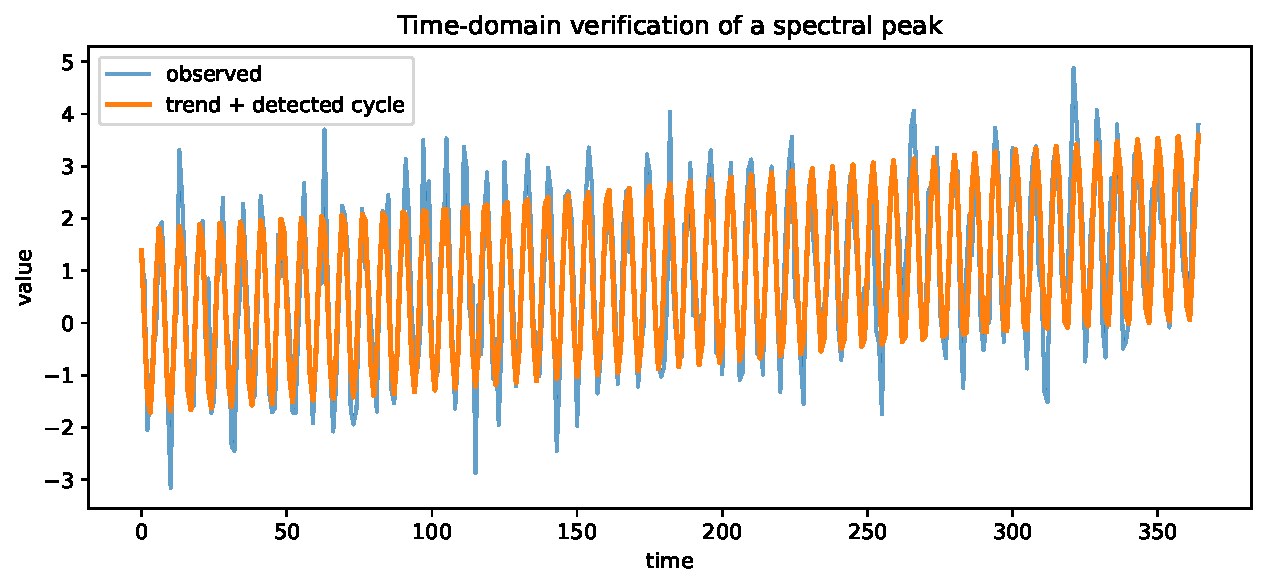
\includegraphics[keepaspectratio]{chapters/chapter-13-dft-fft-periodogram_files/figure-pdf/ch13-periodogram-to-regression-output-2.pdf}}

}

\caption{A periodogram peak can be converted into sine/cosine regressors
and checked by residual diagnostics.}

\end{figure}%

\pandocbounded{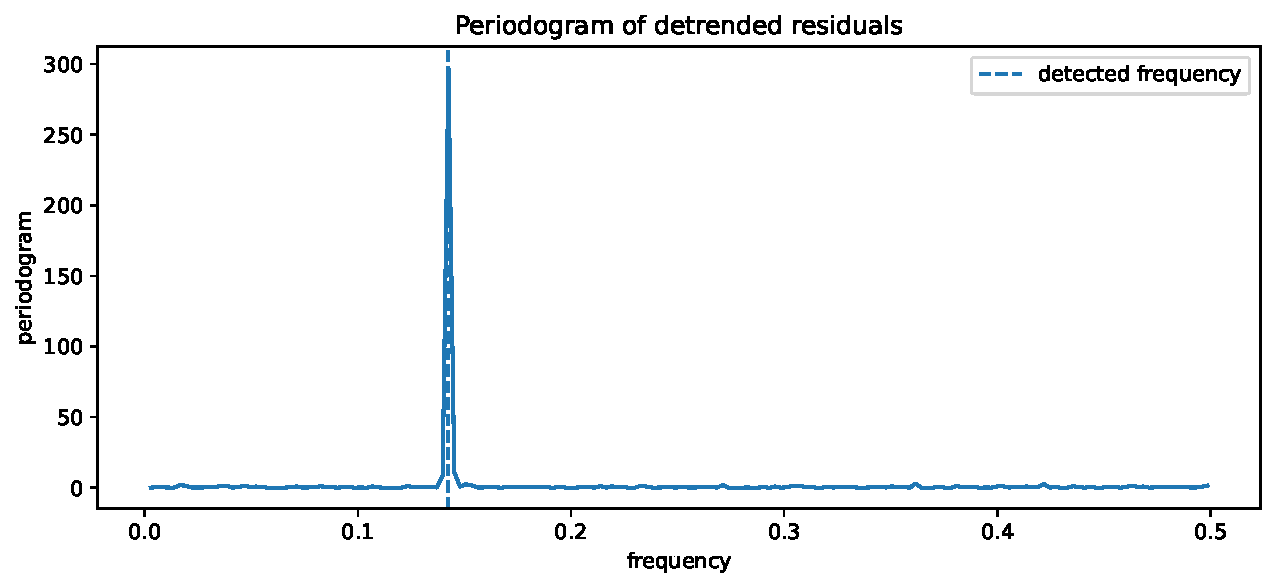
\includegraphics[keepaspectratio]{chapters/chapter-13-dft-fft-periodogram_files/figure-pdf/ch13-periodogram-to-regression-output-3.pdf}}

\pandocbounded{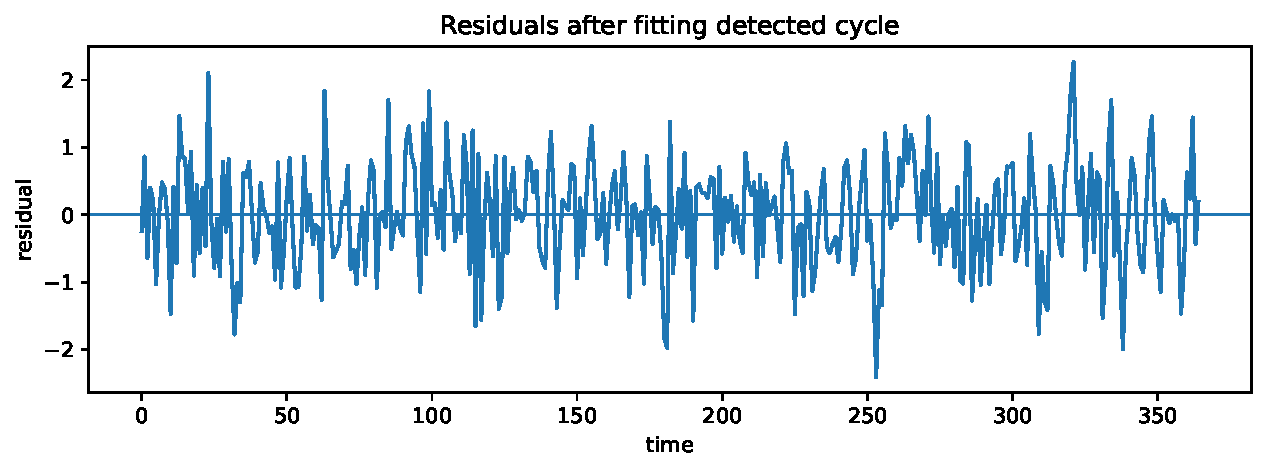
\includegraphics[keepaspectratio]{chapters/chapter-13-dft-fft-periodogram_files/figure-pdf/ch13-periodogram-to-regression-output-4.pdf}}

\section{13.12 Periodogram for stochastic
processes}\label{periodogram-for-stochastic-processes}

For a stationary stochastic process, the periodogram is random. Even if
the true spectrum is smooth, the observed periodogram can be very
irregular.

For example, white noise has a flat spectral density. But the
periodogram of one white-noise realization is not flat. It has random
spikes. Those spikes do not necessarily indicate meaningful periodicity.

This is one of the most common mistakes in spectral analysis:
overinterpreting peaks from a short noisy sequence.

\subsection{Python: white noise has random periodogram
peaks}\label{python-white-noise-has-random-periodogram-peaks}

\begin{Shaded}
\begin{Highlighting}[]
\NormalTok{rng }\OperatorTok{=}\NormalTok{ np.random.default\_rng(}\DecValTok{21}\NormalTok{)}
\NormalTok{n }\OperatorTok{=} \DecValTok{256}
\NormalTok{x }\OperatorTok{=}\NormalTok{ rng.normal(size}\OperatorTok{=}\NormalTok{n)}
\NormalTok{x }\OperatorTok{=}\NormalTok{ x }\OperatorTok{{-}}\NormalTok{ x.mean()}

\NormalTok{freq }\OperatorTok{=}\NormalTok{ np.fft.rfftfreq(n, d}\OperatorTok{=}\DecValTok{1}\NormalTok{)}
\NormalTok{I }\OperatorTok{=}\NormalTok{ np.}\BuiltInTok{abs}\NormalTok{(np.fft.rfft(x)) }\OperatorTok{**} \DecValTok{2} \OperatorTok{/}\NormalTok{ n}

\NormalTok{plt.figure(figsize}\OperatorTok{=}\NormalTok{(}\DecValTok{10}\NormalTok{, }\DecValTok{4}\NormalTok{))}
\NormalTok{plt.plot(freq[}\DecValTok{1}\NormalTok{:], I[}\DecValTok{1}\NormalTok{:])}
\NormalTok{plt.xlabel(}\StringTok{"frequency"}\NormalTok{)}
\NormalTok{plt.ylabel(}\StringTok{"periodogram"}\NormalTok{)}
\NormalTok{plt.title(}\StringTok{"Periodogram of one white{-}noise realization"}\NormalTok{)}
\NormalTok{plt.show()}
\end{Highlighting}
\end{Shaded}

\begin{figure}[H]

{\centering \pandocbounded{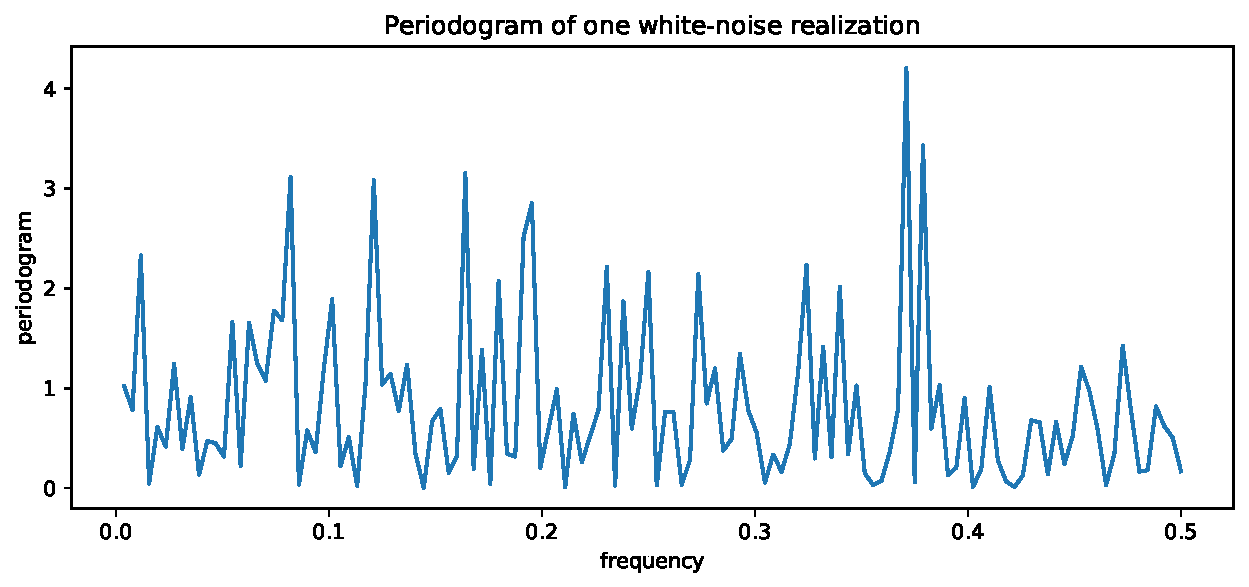
\includegraphics[keepaspectratio]{chapters/chapter-13-dft-fft-periodogram_files/figure-pdf/ch13-white-noise-periodogram-output-1.pdf}}

}

\caption{A white-noise series has a flat spectrum in theory, but its
finite-sample periodogram is noisy.}

\end{figure}%

\begin{tcolorbox}[enhanced jigsaw, arc=.35mm, bottomrule=.15mm, bottomtitle=1mm, breakable, colback=white, colbacktitle=quarto-callout-tip-color!10!white, colframe=quarto-callout-tip-color-frame, coltitle=black, left=2mm, leftrule=.75mm, opacityback=0, opacitybacktitle=0.6, rightrule=.15mm, title=\textcolor{quarto-callout-tip-color}{\faLightbulb}\hspace{0.5em}{Interpretation rule}, titlerule=0mm, toprule=.15mm, toptitle=1mm]

A periodogram peak is a hypothesis generator. It says: ``This frequency
may matter.'' It does not, by itself, prove that the process contains a
deterministic cycle.

\end{tcolorbox}

\section{13.13 Connection with linear
filters}\label{connection-with-linear-filters}

A linear filter transforms a time series by

\[
y_t=\sum_{j=-\infty}^{\infty}a_j x_{t-j}.
\]

In the frequency domain, filtering is multiplication. If the input has
spectral density \(f_x(\omega)\), then under suitable conditions the
output has spectral density

\[
f_y(\omega)=|A(\omega)|^2 f_x(\omega),
\]

where

\[
A(\omega)=\sum_j a_j e^{-2\pi i\omega j}
\]

is the frequency response of the filter.

This explains why moving averages smooth time series. A simple moving
average suppresses high-frequency variation and preserves low-frequency
variation. In the next chapter, we will use this idea to study filters
and wavelets.

\section{13.14 AI-assisted spectral
analysis}\label{ai-assisted-spectral-analysis}

AI tools are useful for planning and checking spectral analysis, but
they should not replace mathematical verification.

\subsection{Good AI uses}\label{good-ai-uses}

Ask an AI assistant to:

\begin{itemize}
\tightlist
\item
  translate a periodogram peak into a candidate period;
\item
  suggest whether centering, detrending, or differencing is appropriate;
\item
  explain why a raw periodogram is jagged;
\item
  generate code for a DFT or FFT calculation;
\item
  compare possible causes of a spectral peak;
\item
  design a residual diagnostic checklist.
\end{itemize}

\subsection{Risky AI uses}\label{risky-ai-uses}

Do not ask an AI assistant to simply ``find the true period'' without
providing:

\begin{itemize}
\tightlist
\item
  the sampling interval;
\item
  whether the data have missing observations;
\item
  whether the data were detrended or differenced;
\item
  whether the peak aligns with a Fourier frequency;
\item
  whether there is leakage or aliasing;
\item
  whether the peak appears in independent validation data.
\end{itemize}

\subsection{Prompt template: spectral
interpretation}\label{prompt-template-spectral-interpretation}

\begin{quote}
I have a time series sampled every {[}time unit{]}. After
centering/detrending, the periodogram has peaks near frequencies
{[}list{]}. Convert these to periods, propose possible interpretations,
and list mathematical checks I should perform before treating them as
real cycles.
\end{quote}

\subsection{Prompt template: code
review}\label{prompt-template-code-review}

\begin{quote}
Review this FFT periodogram code. Check the scaling convention, whether
I centered the data, whether the one-sided frequency axis is correct,
and whether my interpretation of the peak frequency is valid.
\end{quote}

\subsection{AI verification checklist}\label{ai-verification-checklist}

When AI suggests a frequency-domain conclusion, verify:

\begin{enumerate}
\def\labelenumi{\arabic{enumi}.}
\tightlist
\item
  Was the data centered?
\item
  Was trend removed if needed?
\item
  Is the sampling interval known?
\item
  Is the frequency below the Nyquist frequency?
\item
  Is the peak stable under reasonable smoothing?
\item
  Is the peak stable under different windows or train/test splits?
\item
  Does a sine/cosine regression at that frequency improve residual
  diagnostics?
\item
  Does the conclusion make sense in the application domain?
\end{enumerate}

\section{13.15 Common mistakes}\label{common-mistakes-12}

\begin{enumerate}
\def\labelenumi{\arabic{enumi}.}
\tightlist
\item
  \textbf{Forgetting to center the data.} The zero-frequency component
  can dominate the periodogram.
\item
  \textbf{Interpreting trend as periodicity.} Strong trend creates
  low-frequency power.
\item
  \textbf{Confusing frequency and period.} Frequency is cycles per time
  step; period is time steps per cycle.
\item
  \textbf{Ignoring the sampling interval.} A frequency in cycles per
  observation must be converted to cycles per day, week, month, or
  second.
\item
  \textbf{Overinterpreting raw periodogram peaks.} White noise can
  produce random peaks.
\item
  \textbf{Forgetting leakage.} If the true frequency is not on the
  Fourier grid, energy spreads across bins.
\item
  \textbf{Using the FFT as if it were a model.} The FFT is a
  computational transform, not a probabilistic model.
\item
  \textbf{Comparing periodograms with different scaling conventions.}
  Always check how the software defines the DFT and periodogram.
\item
  \textbf{Ignoring missing or irregular sampling.} The standard DFT
  assumes evenly spaced observations.
\item
  \textbf{Skipping residual diagnostics.} A detected frequency should be
  checked in a fitted model.
\end{enumerate}

\section{13.16 Mini project: spectral diagnosis of hidden
seasonality}\label{mini-project-spectral-diagnosis-of-hidden-seasonality}

Choose a real or simulated time series with at least 200 observations.
Suitable examples include electricity demand, temperature, bike sharing,
web traffic, or financial volatility proxies.

Your report should include:

\begin{enumerate}
\def\labelenumi{\arabic{enumi}.}
\tightlist
\item
  a time plot and a short description of visible structure;
\item
  a justification for centering, detrending, differencing, or
  transforming;
\item
  a one-sided periodogram;
\item
  a smoothed periodogram;
\item
  the top three nonzero frequency peaks and their periods;
\item
  a time-domain regression using sine/cosine terms for one selected
  frequency;
\item
  residual diagnostics;
\item
  a paragraph explaining whether the spectral evidence is convincing.
\end{enumerate}

Optional extension: compare the periodogram before and after
differencing. Explain which frequencies become stronger or weaker.

\section{13.17 Exercises}\label{exercises-12}

\subsection{Conceptual exercises}\label{conceptual-exercises-9}

\begin{enumerate}
\def\labelenumi{\arabic{enumi}.}
\tightlist
\item
  Explain why the Fourier frequencies for a sample of length \(n\) are
  \(k/n\).
\item
  Prove that the vectors \[
  \phi_k(t)=n^{-1/2}e^{2\pi i kt/n}
  \] form an orthonormal basis of \(\mathbb C^n\).
\item
  Derive the inverse DFT formula from the Fourier-basis expansion.
\item
  Explain Parseval's identity in words.
\item
  Why does centering remove the zero-frequency spike?
\item
  Why is the periodogram a natural sample analog of the spectral
  density?
\item
  Why is the raw periodogram not usually a consistent estimator of the
  spectral density?
\item
  Explain the bias-variance tradeoff in periodogram smoothing.
\item
  What is spectral leakage? Why does it occur?
\item
  Why is the FFT an algorithm rather than a new mathematical transform?
\end{enumerate}

\subsection{Computational exercises}\label{computational-exercises-6}

\begin{enumerate}
\def\labelenumi{\arabic{enumi}.}
\tightlist
\item
  Write your own direct DFT function and compare it with
  \texttt{np.fft.fft}.
\item
  Simulate a signal with two frequencies and use the periodogram to
  recover them.
\item
  Add increasing amounts of noise and study how peak detection changes.
\item
  Simulate white noise 100 times and record the largest periodogram peak
  each time.
\item
  Compare raw and smoothed periodograms for an AR(1) process with
  \(\phi=0.9\).
\item
  Generate a sinusoid whose frequency is not on the Fourier grid.
  Demonstrate leakage.
\item
  Apply a Hann taper and compare the result with the untapered
  periodogram.
\item
  Fit sine/cosine regressors at the largest periodogram frequency and
  inspect residuals.
\item
  Compare the periodogram of a random walk with the periodogram of its
  first difference.
\item
  Use rolling windows to see whether a dominant frequency changes over
  time.
\end{enumerate}

\subsection{Theory exercises}\label{theory-exercises}

\begin{enumerate}
\def\labelenumi{\arabic{enumi}.}
\tightlist
\item
  Let \(D_k\) be the unnormalized DFT. Show that \[
  \sum_{t=0}^{n-1}|x_t|^2=\frac{1}{n}\sum_{k=0}^{n-1}|D_k|^2.
  \]
\item
  Show that if \(x_t=\cos(2\pi k_0t/n)\) for an integer \(k_0\), then
  the periodogram has nonzero energy only at the paired frequencies
  \(k_0/n\) and \(1-k_0/n\), apart from special cases.
\item
  Suppose \(x_t\) is white noise with variance \(\sigma^2\). What should
  the population spectral density look like? How does one finite
  periodogram differ?
\item
  Let \(y_t=(x_t+x_{t-1})/2\). Derive the frequency response
  \(A(\omega)\) of this moving-average filter.
\item
  Explain why the moving average in Exercise 4 suppresses high
  frequencies.
\end{enumerate}

\section{13.18 Chapter checklist}\label{chapter-checklist-10}

Before moving to filtering and wavelets, make sure you can:

\begin{itemize}
\tightlist
\item[$\square$]
  define Fourier frequencies \(\omega_k=k/n\);
\item[$\square$]
  derive the DFT as a projection onto the Fourier basis;
\item[$\square$]
  explain the difference between \(D_k\), \(c_k\), and \(X(\omega_k)\)
  scaling conventions;
\item[$\square$]
  compute a periodogram using the FFT;
\item[$\square$]
  interpret frequency peaks as candidate periods;
\item[$\square$]
  explain why the periodogram is noisy;
\item[$\square$]
  smooth a periodogram and explain the bias-variance tradeoff;
\item[$\square$]
  identify spectral leakage;
\item[$\square$]
  verify a spectral peak with a time-domain regression;
\item[$\square$]
  use AI assistance while checking centering, scaling, leakage, and
  sampling assumptions.
\end{itemize}

\section{13.19 Looking ahead}\label{looking-ahead-1}

The DFT and periodogram decompose a finite sequence into global sine and
cosine components. This is powerful when periodic behavior is stable
over time. But many modern sequence-data problems involve local changes:
a burst, a regime shift, a transient oscillation, a sudden anomaly, or a
frequency that evolves over time.

The next chapter studies filtering and wavelets. Filters modify the
spectrum, while wavelets localize patterns in both time and frequency.
Together, they extend the Fourier viewpoint toward multiresolution
analysis and modern signal-processing tools for time series.

\chapter{Filtering and Wavelet
Transform}\label{filtering-and-wavelet-transform}

\textbf{Part IV. Frequency-Domain and Multiresolution Methods}\\
\textbf{Chapter goal:} learn how filters reshape a time series in the
time and frequency domains, then extend the idea from global Fourier
frequencies to local time-frequency analysis with wavelets. We use
filters for smoothing, detrending, denoising, transient detection, and
feature extraction for modern forecasting and sequence-learning models.

\section{Learning objectives}\label{learning-objectives-13}

After studying this chapter, you should be able to:

\begin{enumerate}
\def\labelenumi{\arabic{enumi}.}
\tightlist
\item
  define a linear time-invariant filter using convolution and the
  backshift operator;
\item
  distinguish finite impulse response and infinite impulse response
  filters;
\item
  compute the frequency response of a filter and interpret its magnitude
  and phase;
\item
  prove that filtering transforms spectra by
  \(f_Y(\omega)=|A(\omega)|^2 f_X(\omega)\);
\item
  explain moving-average smoothers, difference filters,
  seasonal-difference filters, and band-pass filters;
\item
  understand why Fourier methods can miss local frequency changes;
\item
  define short-time Fourier analysis as a first solution to
  localization;
\item
  explain the Haar wavelet transform and multiresolution decomposition;
\item
  use wavelet coefficients for denoising, compression, change-point
  detection, and feature extraction;
\item
  use AI tools to critique filtering choices, leakage risks, and
  interpretability claims.
\end{enumerate}

\section{14.1 Why filtering?}\label{why-filtering}

In Chapters 12 and 13 we learned that a stationary time series can be
viewed through its frequency content. This chapter asks a complementary
question:

\begin{quote}
How can we transform a time series so that certain frequencies, trends,
or localized events become easier to see?
\end{quote}

A \textbf{filter} is a rule that takes an input series \(\{X_t\}\) and
produces an output series \(\{Y_t\}\). A simple example is the centered
moving average

\[
Y_t=\frac{1}{2m+1}\sum_{j=-m}^m X_{t-j}.
\]

This filter smooths the series by replacing each observation with a
local average. Short-scale variation is reduced; slow variation is
preserved. In frequency language, this is a \textbf{low-pass filter}.

A first difference

\[
Y_t=\nabla X_t=X_t-X_{t-1}
\]

does the opposite: it removes constant levels and emphasizes short-scale
changes. It is a \textbf{high-pass filter}.

Filtering is used for several purposes:

\begin{itemize}
\tightlist
\item
  remove noise before forecasting;
\item
  remove trend or seasonality before fitting stationary models;
\item
  isolate business-cycle or seasonal frequencies;
\item
  detect transients, jumps, bursts, or anomalies;
\item
  construct features for machine-learning models;
\item
  precondition data before deep sequence models.
\end{itemize}

\begin{tcolorbox}[enhanced jigsaw, arc=.35mm, bottomrule=.15mm, bottomtitle=1mm, breakable, colback=white, colbacktitle=quarto-callout-warning-color!10!white, colframe=quarto-callout-warning-color-frame, coltitle=black, left=2mm, leftrule=.75mm, opacityback=0, opacitybacktitle=0.6, rightrule=.15mm, title=\textcolor{quarto-callout-warning-color}{\faExclamationTriangle}\hspace{0.5em}{Filtering changes the problem}, titlerule=0mm, toprule=.15mm, toptitle=1mm]

Filtering is not a neutral preprocessing step. A filtered series has a
different dependence structure from the original series. Before
filtering, ask: Which part of the signal am I trying to preserve, and
which part am I trying to suppress?

\end{tcolorbox}

\section{14.2 Linear time-invariant
filters}\label{linear-time-invariant-filters}

A \textbf{linear time-invariant filter} has the form

\[
Y_t=\sum_{j=-\infty}^{\infty} a_j X_{t-j},
\]

where the sequence \(\{a_j\}\) is called the \textbf{filter kernel},
\textbf{impulse response}, or \textbf{filter coefficients}.

The filter is \textbf{linear} because

\[
L(\alpha X_t+\beta Z_t)=\alpha L(X_t)+\beta L(Z_t),
\]

and it is \textbf{time-invariant} because the same coefficients \(a_j\)
are used at every time \(t\).

A sufficient condition for the sum to be well behaved is absolute
summability:

\[
\sum_{j=-\infty}^{\infty}|a_j|<\infty.
\]

When the filter uses only finitely many coefficients, it is called a
\textbf{finite impulse response} filter, or FIR filter. When infinitely
many coefficients are used, it is called an \textbf{infinite impulse
response} filter, or IIR filter.

\subsection{Backshift notation}\label{backshift-notation}

Using the backshift operator \(B X_t=X_{t-1}\), we can write

\[
Y_t=a(B)X_t,
\]

where

\[
a(B)=\sum_{j=-\infty}^{\infty}a_jB^j.
\]

For example, the first-difference filter is

\[
\nabla X_t=(1-B)X_t.
\]

The seasonal-difference filter with period \(s\) is

\[
\nabla_s X_t=(1-B^s)X_t=X_t-X_{t-s}.
\]

The centered three-point moving average is

\[
Y_t=\frac{1}{3}(X_{t-1}+X_t+X_{t+1})
=\left(\frac{1}{3}B+\frac{1}{3}+\frac{1}{3}B^{-1}\right)X_t.
\]

\begin{tcolorbox}[enhanced jigsaw, arc=.35mm, bottomrule=.15mm, bottomtitle=1mm, breakable, colback=white, colbacktitle=quarto-callout-note-color!10!white, colframe=quarto-callout-note-color-frame, coltitle=black, left=2mm, leftrule=.75mm, opacityback=0, opacitybacktitle=0.6, rightrule=.15mm, title=\textcolor{quarto-callout-note-color}{\faInfo}\hspace{0.5em}{Causal versus centered filters}, titlerule=0mm, toprule=.15mm, toptitle=1mm]

A forecasting filter must be causal: it can use \(X_t,X_{t-1},\ldots\)
but not future values. A centered smoother is useful for retrospective
visualization, but it leaks future information if used inside a
forecasting pipeline.

\end{tcolorbox}

\section{14.3 Frequency response}\label{frequency-response}

To understand a filter, feed it a complex sinusoid

\[
X_t=e^{2\pi i\omega t}.
\]

Then

\[
\begin{aligned}
Y_t
&=\sum_j a_j X_{t-j} \\
&=\sum_j a_j e^{2\pi i\omega(t-j)} \\
&=e^{2\pi i\omega t}\sum_j a_j e^{-2\pi i\omega j}.
\end{aligned}
\]

Thus the sinusoid remains at the same frequency. Only its amplitude and
phase are changed. The multiplier

\[
A(\omega)=\sum_{j=-\infty}^{\infty}a_j e^{-2\pi i\omega j}
\]

is called the \textbf{frequency response} of the filter.

The magnitude

\[
|A(\omega)|
\]

measures how much the filter amplifies or attenuates frequency
\(\omega\). The squared magnitude

\[
|A(\omega)|^2
\]

measures the effect on power or variance at frequency \(\omega\).

The phase

\[
\arg A(\omega)
\]

measures how much the filter shifts that frequency component in time.

\subsection{Examples}\label{examples-1}

The first-difference filter has coefficients \(a_0=1\) and \(a_1=-1\).
Therefore,

\[
A(\omega)=1-e^{-2\pi i\omega}.
\]

Using \(|1-e^{-ix}|^2=2-2\cos x=4\sin^2(x/2)\), we get

\[
|A(\omega)|^2=4\sin^2(\pi\omega).
\]

At \(\omega=0\), the response is \(0\), so differencing removes constant
components. At \(\omega=1/2\), the response is \(4\), so high-frequency
oscillations are amplified.

For the two-sided moving average with window \(2m+1\),

\[
a_j=\frac{1}{2m+1},\qquad j=-m,\ldots,m.
\]

The response is

\[
A(\omega)=\frac{1}{2m+1}\sum_{j=-m}^{m}e^{-2\pi i\omega j}.
\]

This response is large near \(\omega=0\) and small at many higher
frequencies, so the filter smooths the series.

\section{14.4 Filtering and spectral
density}\label{filtering-and-spectral-density}

Suppose \(\{X_t\}\) is a zero-mean stationary time series with spectral
density \(f_X(\omega)\), and define

\[
Y_t=\sum_j a_jX_{t-j}.
\]

Then the output process \(\{Y_t\}\) has spectral density

\[
f_Y(\omega)=|A(\omega)|^2f_X(\omega).
\]

This formula is one of the central results of frequency-domain
time-series analysis.

\subsection{Derivation}\label{derivation}

The autocovariance of \(Y_t\) is

\[
\begin{aligned}
\gamma_Y(h)
&=\operatorname{Cov}(Y_{t+h},Y_t)\\
&=\operatorname{Cov}\left(\sum_j a_jX_{t+h-j},\sum_k a_kX_{t-k}\right)\\
&=\sum_j\sum_k a_ja_k\gamma_X(h-j+k).
\end{aligned}
\]

Taking the Fourier transform gives

\[
\begin{aligned}
f_Y(\omega)
&=\sum_h \gamma_Y(h)e^{-2\pi i\omega h}\\
&=\sum_h\sum_j\sum_k a_ja_k\gamma_X(h-j+k)e^{-2\pi i\omega h}.
\end{aligned}
\]

Let \(r=h-j+k\), so \(h=r+j-k\). Then

\[
\begin{aligned}
f_Y(\omega)
&=\sum_j\sum_k a_ja_k e^{-2\pi i\omega(j-k)}
\sum_r \gamma_X(r)e^{-2\pi i\omega r}\\
&=\left(\sum_j a_je^{-2\pi i\omega j}\right)
\left(\sum_k a_ke^{2\pi i\omega k}\right)f_X(\omega)\\
&=A(\omega)\overline{A(\omega)}f_X(\omega)\\
&=|A(\omega)|^2f_X(\omega).
\end{aligned}
\]

\begin{tcolorbox}[enhanced jigsaw, arc=.35mm, bottomrule=.15mm, bottomtitle=1mm, breakable, colback=white, colbacktitle=quarto-callout-important-color!10!white, colframe=quarto-callout-important-color-frame, coltitle=black, left=2mm, leftrule=.75mm, opacityback=0, opacitybacktitle=0.6, rightrule=.15mm, title=\textcolor{quarto-callout-important-color}{\faExclamation}\hspace{0.5em}{Filter design principle}, titlerule=0mm, toprule=.15mm, toptitle=1mm]

To suppress a frequency band, make \(|A(\omega)|^2\) small on that band.
To preserve a frequency band, make \(|A(\omega)|^2\) close to \(1\) on
that band.

\end{tcolorbox}

\section{14.5 Common filters in time-series
analysis}\label{common-filters-in-time-series-analysis}

\subsection{Moving-average smoother}\label{moving-average-smoother}

A trailing moving average of length \(m\) is

\[
Y_t=\frac{1}{m}\sum_{j=0}^{m-1}X_{t-j}.
\]

It is causal and therefore can be used in real time. However, it
introduces a delay because it averages current and past observations.

A centered moving average is

\[
Y_t=\frac{1}{2m+1}\sum_{j=-m}^{m}X_{t-j}.
\]

It is symmetric and has no phase distortion, but it uses future values
and therefore should not be used to create forecasting features unless
it is computed only inside the training window and with careful leakage
prevention.

\subsection{Difference filter}\label{difference-filter}

The first difference

\[
Y_t=X_t-X_{t-1}
\]

removes constants and weakens low-frequency trend. In ARIMA notation,
this is \(\nabla X_t=(1-B)X_t\).

The second difference

\[
\nabla^2X_t=X_t-2X_{t-1}+X_{t-2}
\]

removes linear trends.

\subsection{Seasonal-difference
filter}\label{seasonal-difference-filter}

For seasonal period \(s\),

\[
Y_t=X_t-X_{t-s}.
\]

The response is

\[
A(\omega)=1-e^{-2\pi i\omega s},
\]

so

\[
|A(\omega)|^2=4\sin^2(\pi s\omega).
\]

This filter removes components at frequencies

\[
\omega=0,\frac{1}{s},\frac{2}{s},\ldots,
\]

up to aliases on the discrete frequency grid.

\subsection{Exponential smoothing as an IIR
filter}\label{exponential-smoothing-as-an-iir-filter}

Simple exponential smoothing is

\[
Y_t=\alpha X_t+(1-\alpha)Y_{t-1},\qquad 0<\alpha<1.
\]

Iterating gives

\[
Y_t=\alpha\sum_{j=0}^{\infty}(1-\alpha)^jX_{t-j}.
\]

Thus exponential smoothing is a causal IIR low-pass filter with
geometrically decaying weights.

\section{14.6 Interactive HTML: smoothing, differencing, and frequency
response}\label{interactive-html-smoothing-differencing-and-frequency-response}

The following interactive module shows the same signal before and after
two common filters. The raw signal contains a slow component, a fast
component, and noise. The moving-average filter suppresses fast
variation. The difference filter suppresses slow variation.

\subsection{Interactive filter
explorer}\label{interactive-filter-explorer}

Use the controls to change the moving-average window, the frequency of
the fast component, and the noise level. The second plot shows the
theoretical magnitude-squared response of the moving-average and
first-difference filters.

Moving-average window
\protect\phantomsection\label{ch14-ma-window-value}{13} Fast frequency
\protect\phantomsection\label{ch14-fast-frequency-value}{0.22} Noise
level \protect\phantomsection\label{ch14-noise-level-value}{0.35}

\protect\phantomsection\label{ch14-filter-time-plot}

\protect\phantomsection\label{ch14-filter-response-plot}

\section{14.7 Python: filtering and frequency
response}\label{python-filtering-and-frequency-response}

\protect\phantomsection\label{ch14-filtering-example}
\begin{Shaded}
\begin{Highlighting}[]
\ImportTok{import}\NormalTok{ numpy }\ImportTok{as}\NormalTok{ np}
\ImportTok{import}\NormalTok{ matplotlib.pyplot }\ImportTok{as}\NormalTok{ plt}

\NormalTok{rng }\OperatorTok{=}\NormalTok{ np.random.default\_rng(}\DecValTok{7339}\NormalTok{)}
\NormalTok{n }\OperatorTok{=} \DecValTok{240}
\NormalTok{t }\OperatorTok{=}\NormalTok{ np.arange(n)}
\NormalTok{slow }\OperatorTok{=} \FloatTok{1.4} \OperatorTok{*}\NormalTok{ np.sin(}\DecValTok{2} \OperatorTok{*}\NormalTok{ np.pi }\OperatorTok{*} \FloatTok{0.025} \OperatorTok{*}\NormalTok{ t)}
\NormalTok{fast }\OperatorTok{=} \FloatTok{0.45} \OperatorTok{*}\NormalTok{ np.sin(}\DecValTok{2} \OperatorTok{*}\NormalTok{ np.pi }\OperatorTok{*} \FloatTok{0.22} \OperatorTok{*}\NormalTok{ t)}
\NormalTok{noise }\OperatorTok{=} \FloatTok{0.35} \OperatorTok{*}\NormalTok{ rng.normal(size}\OperatorTok{=}\NormalTok{n)}
\NormalTok{x }\OperatorTok{=}\NormalTok{ slow }\OperatorTok{+}\NormalTok{ fast }\OperatorTok{+}\NormalTok{ noise}

\NormalTok{m }\OperatorTok{=} \DecValTok{13}
\NormalTok{kernel }\OperatorTok{=}\NormalTok{ np.ones(m) }\OperatorTok{/}\NormalTok{ m}
\NormalTok{ma }\OperatorTok{=}\NormalTok{ np.convolve(x, kernel, mode}\OperatorTok{=}\StringTok{"same"}\NormalTok{)}
\NormalTok{diff }\OperatorTok{=}\NormalTok{ np.r\_[np.nan, np.diff(x)]}

\NormalTok{plt.figure(figsize}\OperatorTok{=}\NormalTok{(}\DecValTok{10}\NormalTok{, }\DecValTok{4}\NormalTok{))}
\NormalTok{plt.plot(t, x, label}\OperatorTok{=}\StringTok{"raw"}\NormalTok{, alpha}\OperatorTok{=}\FloatTok{0.6}\NormalTok{)}
\NormalTok{plt.plot(t, ma, label}\OperatorTok{=}\StringTok{"centered moving average"}\NormalTok{)}
\NormalTok{plt.plot(t, slow, label}\OperatorTok{=}\StringTok{"slow component"}\NormalTok{, linestyle}\OperatorTok{=}\StringTok{"{-}{-}"}\NormalTok{)}
\NormalTok{plt.xlabel(}\StringTok{"time"}\NormalTok{)}
\NormalTok{plt.ylabel(}\StringTok{"value"}\NormalTok{)}
\NormalTok{plt.title(}\StringTok{"Low{-}pass smoothing with a moving{-}average filter"}\NormalTok{)}
\NormalTok{plt.legend()}
\NormalTok{plt.show()}

\NormalTok{plt.figure(figsize}\OperatorTok{=}\NormalTok{(}\DecValTok{10}\NormalTok{, }\DecValTok{3}\NormalTok{))}
\NormalTok{plt.plot(t, diff, label}\OperatorTok{=}\StringTok{"first difference"}\NormalTok{)}
\NormalTok{plt.xlabel(}\StringTok{"time"}\NormalTok{)}
\NormalTok{plt.ylabel(}\StringTok{"difference"}\NormalTok{)}
\NormalTok{plt.title(}\StringTok{"High{-}pass behavior of the first{-}difference filter"}\NormalTok{)}
\NormalTok{plt.legend()}
\NormalTok{plt.show()}
\end{Highlighting}
\end{Shaded}

\begin{figure}[H]

{\centering \pandocbounded{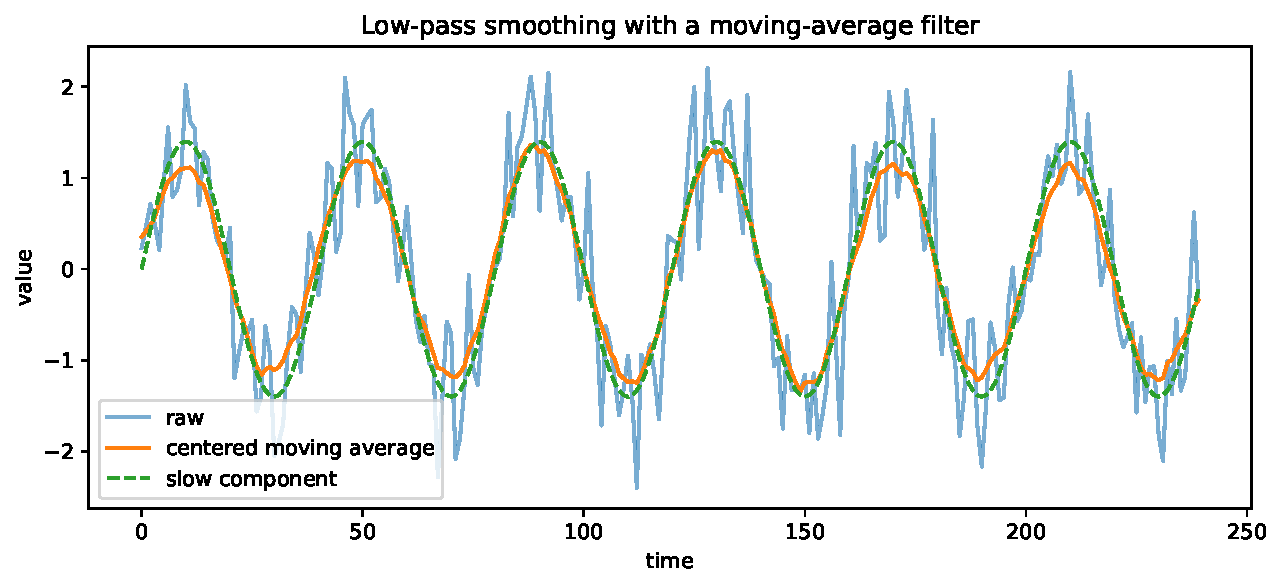
\includegraphics[keepaspectratio]{chapters/chapter-14-filtering-wavelets_files/figure-pdf/ch14-filtering-example-output-1.pdf}}

}

\caption{A moving-average filter suppresses high-frequency variation,
while differencing emphasizes short-scale changes.}

\end{figure}%

\pandocbounded{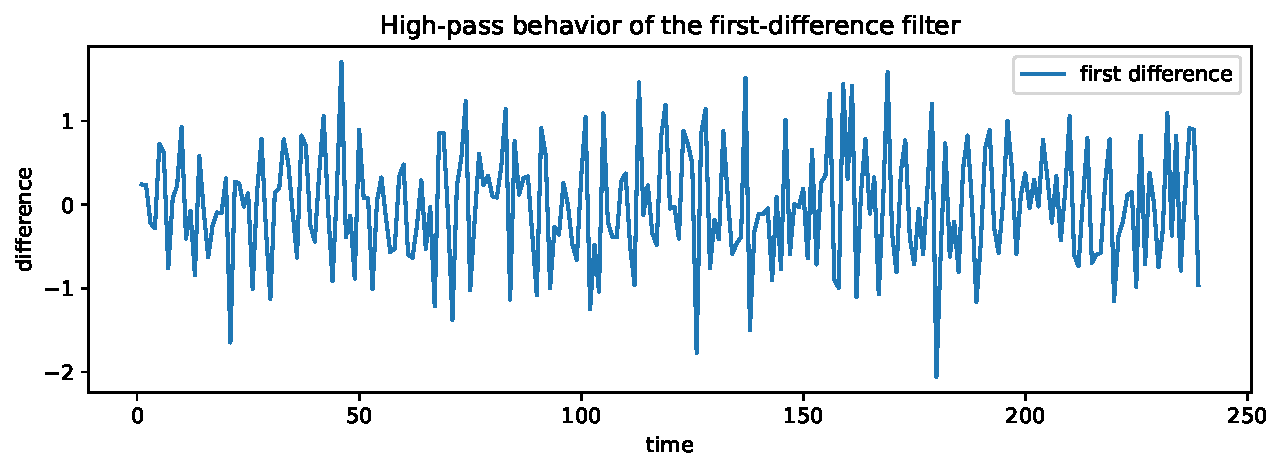
\includegraphics[keepaspectratio]{chapters/chapter-14-filtering-wavelets_files/figure-pdf/ch14-filtering-example-output-2.pdf}}

\begin{Shaded}
\begin{Highlighting}[]
\NormalTok{omega }\OperatorTok{=}\NormalTok{ np.linspace(}\DecValTok{0}\NormalTok{, }\FloatTok{0.5}\NormalTok{, }\DecValTok{800}\NormalTok{)}

\KeywordTok{def}\NormalTok{ moving\_average\_response(omega, m):}
    \CommentTok{\# H(omega) = (1/m) sum\_\{j=0\}\^{}\{m{-}1\} exp({-}2 pi i omega j)}
\NormalTok{    response }\OperatorTok{=}\NormalTok{ np.zeros\_like(omega, dtype}\OperatorTok{=}\BuiltInTok{complex}\NormalTok{)}
    \ControlFlowTok{for}\NormalTok{ j }\KeywordTok{in} \BuiltInTok{range}\NormalTok{(m):}
\NormalTok{        response }\OperatorTok{+=}\NormalTok{ np.exp(}\OperatorTok{{-}}\OtherTok{2j} \OperatorTok{*}\NormalTok{ np.pi }\OperatorTok{*}\NormalTok{ omega }\OperatorTok{*}\NormalTok{ j) }\OperatorTok{/}\NormalTok{ m}
    \ControlFlowTok{return}\NormalTok{ response}

\NormalTok{A\_ma }\OperatorTok{=}\NormalTok{ moving\_average\_response(omega, m}\OperatorTok{=}\DecValTok{13}\NormalTok{)}
\NormalTok{A\_diff }\OperatorTok{=} \DecValTok{1} \OperatorTok{{-}}\NormalTok{ np.exp(}\OperatorTok{{-}}\OtherTok{2j} \OperatorTok{*}\NormalTok{ np.pi }\OperatorTok{*}\NormalTok{ omega)}
\NormalTok{A\_seasonal }\OperatorTok{=} \DecValTok{1} \OperatorTok{{-}}\NormalTok{ np.exp(}\OperatorTok{{-}}\OtherTok{2j} \OperatorTok{*}\NormalTok{ np.pi }\OperatorTok{*} \DecValTok{12} \OperatorTok{*}\NormalTok{ omega)}

\NormalTok{plt.figure(figsize}\OperatorTok{=}\NormalTok{(}\DecValTok{9}\NormalTok{, }\DecValTok{4}\NormalTok{))}
\NormalTok{plt.plot(omega, np.}\BuiltInTok{abs}\NormalTok{(A\_ma) }\OperatorTok{**} \DecValTok{2}\NormalTok{, label}\OperatorTok{=}\StringTok{"MA(13) smoother"}\NormalTok{)}
\NormalTok{plt.plot(omega, np.}\BuiltInTok{abs}\NormalTok{(A\_diff) }\OperatorTok{**} \DecValTok{2}\NormalTok{, label}\OperatorTok{=}\StringTok{"first difference"}\NormalTok{)}
\NormalTok{plt.plot(omega, np.}\BuiltInTok{abs}\NormalTok{(A\_seasonal) }\OperatorTok{**} \DecValTok{2}\NormalTok{, label}\OperatorTok{=}\StringTok{"seasonal difference, s=12"}\NormalTok{)}
\NormalTok{plt.xlabel(}\StringTok{"frequency ω"}\NormalTok{)}
\NormalTok{plt.ylabel(}\StringTok{"squared gain |A(ω)|²"}\NormalTok{)}
\NormalTok{plt.title(}\StringTok{"Frequency responses of three filters"}\NormalTok{)}
\NormalTok{plt.legend()}
\NormalTok{plt.show()}
\end{Highlighting}
\end{Shaded}

\begin{figure}[H]

{\centering \pandocbounded{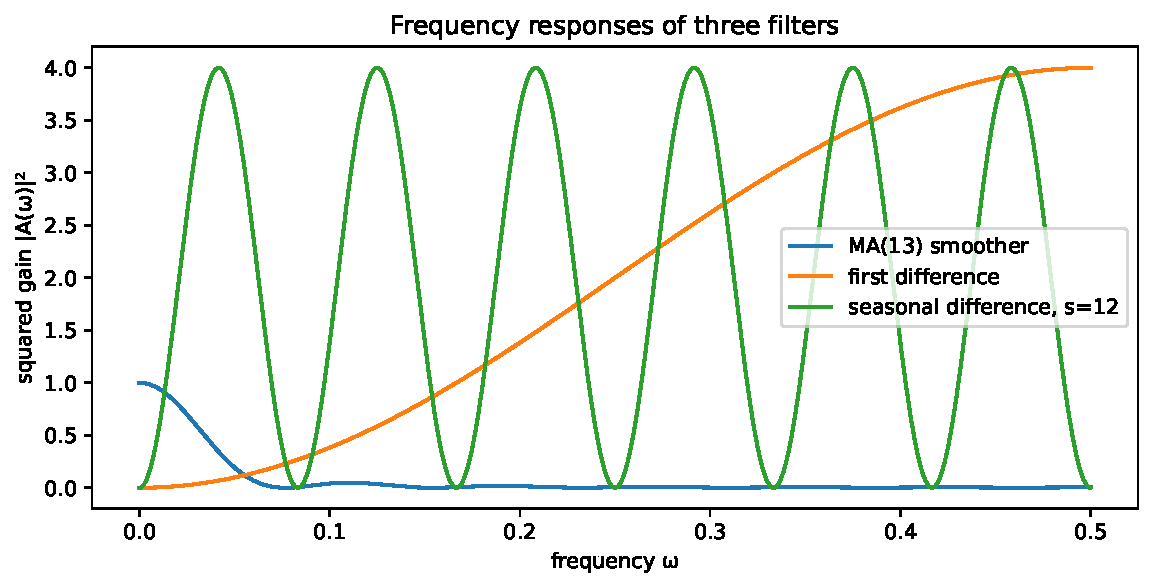
\includegraphics[keepaspectratio]{chapters/chapter-14-filtering-wavelets_files/figure-pdf/ch14-frequency-response-python-output-1.pdf}}

}

\caption{Magnitude-squared responses of common filters.}

\end{figure}%

\section{14.8 Filters, leakage, and forecasting
validation}\label{filters-leakage-and-forecasting-validation}

Filtering can introduce \textbf{look-ahead leakage}. Suppose the goal is
to forecast \(X_{t+1}\) from information available at time \(t\). If we
create a centered moving-average feature

\[
Z_t=\frac{1}{3}(X_{t-1}+X_t+X_{t+1}),
\]

then \(Z_t\) contains the future value \(X_{t+1}\). A
supervised-learning model trained on \(Z_t\) is given information that
would not be available at prediction time.

For forecasting, causal features are safer:

\[
Z_t=\frac{1}{m}\sum_{j=0}^{m-1}X_{t-j}.
\]

Even then, validation must respect time order. The filter must be fit or
applied inside each training window, and no operation should use future
observations when producing training or validation features.

\begin{tcolorbox}[enhanced jigsaw, arc=.35mm, bottomrule=.15mm, bottomtitle=1mm, breakable, colback=white, colbacktitle=quarto-callout-important-color!10!white, colframe=quarto-callout-important-color-frame, coltitle=black, left=2mm, leftrule=.75mm, opacityback=0, opacitybacktitle=0.6, rightrule=.15mm, title=\textcolor{quarto-callout-important-color}{\faExclamation}\hspace{0.5em}{Practical rule}, titlerule=0mm, toprule=.15mm, toptitle=1mm]

For exploratory plots, centered smoothers are often acceptable. For
forecasting features, use causal filters unless you can prove that no
future information enters the feature construction.

\end{tcolorbox}

\section{14.9 From Fourier to local time-frequency
analysis}\label{from-fourier-to-local-time-frequency-analysis}

The Fourier transform represents a series using global sinusoids. This
works well when frequency content is stable over time. But many real
sequences are \textbf{nonstationary in frequency}:

\begin{itemize}
\tightlist
\item
  a machine sensor develops a high-frequency vibration only near
  failure;
\item
  an ECG signal has local transient events;
\item
  a financial return series has short bursts of volatility;
\item
  a traffic series changes its weekly pattern after a disruption;
\item
  a speech signal changes frequency content from phoneme to phoneme.
\end{itemize}

A single periodogram tells us which frequencies are present overall, but
not when they occur.

\subsection{Short-time Fourier
transform}\label{short-time-fourier-transform}

A natural solution is to compute Fourier transforms on local windows.
Given a window function \(g\), the short-time Fourier transform is

\[
\operatorname{STFT}_x(u,\omega)
=\sum_t x_t g(t-u)e^{-2\pi i\omega t}.
\]

The parameter \(u\) localizes time, and \(\omega\) localizes frequency.
The squared magnitude

\[
|\operatorname{STFT}_x(u,\omega)|^2
\]

is a local time-frequency energy measure.

The limitation is that the window width is fixed. A narrow window gives
good time resolution but poor frequency resolution. A wide window gives
good frequency resolution but poor time resolution.

Wavelets address this by changing the window width with scale.

\section{14.10 Wavelets and multiresolution
analysis}\label{wavelets-and-multiresolution-analysis}

A \textbf{wavelet} is a localized oscillatory function. Unlike a sine
wave, which extends forever, a wavelet is concentrated in time.

Starting from a mother wavelet \(\psi(t)\), define scaled and translated
wavelets by

\[
\psi_{a,b}(t)=\frac{1}{\sqrt{|a|}}\psi\left(\frac{t-b}{a}\right),
\]

where \(a\) is scale and \(b\) is location.

\begin{itemize}
\tightlist
\item
  Small \(a\): compressed wavelet, good for high-frequency local events.
\item
  Large \(a\): stretched wavelet, good for low-frequency broad behavior.
\end{itemize}

The continuous wavelet transform is

\[
W_x(a,b)=\int x(t)\overline{\psi_{a,b}(t)}\,dt.
\]

For discrete data, we often use dyadic scales \(a=2^j\) and translations
aligned with the sample grid. This leads to the discrete wavelet
transform.

\begin{tcolorbox}[enhanced jigsaw, arc=.35mm, bottomrule=.15mm, bottomtitle=1mm, breakable, colback=white, colbacktitle=quarto-callout-note-color!10!white, colframe=quarto-callout-note-color-frame, coltitle=black, left=2mm, leftrule=.75mm, opacityback=0, opacitybacktitle=0.6, rightrule=.15mm, title=\textcolor{quarto-callout-note-color}{\faInfo}\hspace{0.5em}{Wavelet idea}, titlerule=0mm, toprule=.15mm, toptitle=1mm]

Fourier analysis asks: how much frequency \(\omega\) is present in the
whole signal? Wavelet analysis asks: how much scale \(a\) is present
near time \(b\)?

\end{tcolorbox}

\section{14.11 The Haar wavelet}\label{the-haar-wavelet}

The simplest wavelet is the \textbf{Haar wavelet}:

\[
\psi(t)=
\begin{cases}
1, & 0\leq t<1/2,\\
-1, & 1/2\leq t<1,\\
0, & \text{otherwise.}
\end{cases}
\]

For a pair of observations \((x_0,x_1)\), the Haar transform computes

\[
a=\frac{x_0+x_1}{\sqrt 2},
\qquad
 d=\frac{x_0-x_1}{\sqrt 2}.
\]

The coefficient \(a\) is an average, and \(d\) is a detail. The inverse
transform is

\[
x_0=\frac{a+d}{\sqrt 2},
\qquad
x_1=\frac{a-d}{\sqrt 2}.
\]

For a longer sequence of length \(n=2^J\), the Haar transform repeatedly
averages neighboring pairs and stores the differences. This gives a
multiresolution representation:

\[
\text{data} = \text{coarse approximation} + \text{details at several scales}.
\]

The Haar transform is orthonormal, so it preserves energy:

\[
\sum_t x_t^2 = \sum_k c_k^2,
\]

where \(c_k\) are the wavelet coefficients.

\section{14.12 Python: Haar wavelet transform from
scratch}\label{python-haar-wavelet-transform-from-scratch}

The next code block implements a simple orthonormal Haar transform. This
avoids hiding the mathematics inside a library.

\begin{Shaded}
\begin{Highlighting}[]
\ImportTok{import}\NormalTok{ numpy }\ImportTok{as}\NormalTok{ np}
\ImportTok{import}\NormalTok{ matplotlib.pyplot }\ImportTok{as}\NormalTok{ plt}


\KeywordTok{def}\NormalTok{ haar\_transform(x):}
    \CommentTok{"""Return the orthonormal Haar wavelet coefficients of a length{-}2\^{}J vector."""}
\NormalTok{    x }\OperatorTok{=}\NormalTok{ np.asarray(x, dtype}\OperatorTok{=}\BuiltInTok{float}\NormalTok{).copy()}
\NormalTok{    n }\OperatorTok{=} \BuiltInTok{len}\NormalTok{(x)}
\NormalTok{    coeffs }\OperatorTok{=}\NormalTok{ []}
\NormalTok{    current }\OperatorTok{=}\NormalTok{ x.copy()}
    \ControlFlowTok{while} \BuiltInTok{len}\NormalTok{(current) }\OperatorTok{\textgreater{}} \DecValTok{1}\NormalTok{:}
\NormalTok{        avg }\OperatorTok{=}\NormalTok{ (current[}\DecValTok{0}\NormalTok{::}\DecValTok{2}\NormalTok{] }\OperatorTok{+}\NormalTok{ current[}\DecValTok{1}\NormalTok{::}\DecValTok{2}\NormalTok{]) }\OperatorTok{/}\NormalTok{ np.sqrt(}\DecValTok{2}\NormalTok{)}
\NormalTok{        detail }\OperatorTok{=}\NormalTok{ (current[}\DecValTok{0}\NormalTok{::}\DecValTok{2}\NormalTok{] }\OperatorTok{{-}}\NormalTok{ current[}\DecValTok{1}\NormalTok{::}\DecValTok{2}\NormalTok{]) }\OperatorTok{/}\NormalTok{ np.sqrt(}\DecValTok{2}\NormalTok{)}
\NormalTok{        coeffs.append(detail)}
\NormalTok{        current }\OperatorTok{=}\NormalTok{ avg}
\NormalTok{    coeffs.append(current)}
    \CommentTok{\# Store as [coarsest average, finest{-}to{-}coarsest details reversed]}
    \ControlFlowTok{return}\NormalTok{ coeffs[}\OperatorTok{{-}}\DecValTok{1}\NormalTok{], coeffs[}\OperatorTok{{-}}\DecValTok{2}\NormalTok{::}\OperatorTok{{-}}\DecValTok{1}\NormalTok{]}


\KeywordTok{def}\NormalTok{ inverse\_haar\_transform(coarse, details):}
    \CommentTok{"""Invert coefficients returned by haar\_transform."""}
\NormalTok{    current }\OperatorTok{=}\NormalTok{ np.asarray(coarse, dtype}\OperatorTok{=}\BuiltInTok{float}\NormalTok{)}
    \ControlFlowTok{for}\NormalTok{ detail }\KeywordTok{in}\NormalTok{ details:}
\NormalTok{        detail }\OperatorTok{=}\NormalTok{ np.asarray(detail, dtype}\OperatorTok{=}\BuiltInTok{float}\NormalTok{)}
\NormalTok{        out }\OperatorTok{=}\NormalTok{ np.empty(current.size }\OperatorTok{*} \DecValTok{2}\NormalTok{)}
\NormalTok{        out[}\DecValTok{0}\NormalTok{::}\DecValTok{2}\NormalTok{] }\OperatorTok{=}\NormalTok{ (current }\OperatorTok{+}\NormalTok{ detail) }\OperatorTok{/}\NormalTok{ np.sqrt(}\DecValTok{2}\NormalTok{)}
\NormalTok{        out[}\DecValTok{1}\NormalTok{::}\DecValTok{2}\NormalTok{] }\OperatorTok{=}\NormalTok{ (current }\OperatorTok{{-}}\NormalTok{ detail) }\OperatorTok{/}\NormalTok{ np.sqrt(}\DecValTok{2}\NormalTok{)}
\NormalTok{        current }\OperatorTok{=}\NormalTok{ out}
    \ControlFlowTok{return}\NormalTok{ current}

\NormalTok{n }\OperatorTok{=} \DecValTok{256}
\NormalTok{t }\OperatorTok{=}\NormalTok{ np.arange(n)}
\NormalTok{clean }\OperatorTok{=}\NormalTok{ np.sin(}\DecValTok{2} \OperatorTok{*}\NormalTok{ np.pi }\OperatorTok{*}\NormalTok{ t }\OperatorTok{/} \DecValTok{64}\NormalTok{)}
\NormalTok{clean }\OperatorTok{+=} \FloatTok{0.7} \OperatorTok{*}\NormalTok{ ((t }\OperatorTok{\textgreater{}=} \DecValTok{110}\NormalTok{) }\OperatorTok{\&}\NormalTok{ (t }\OperatorTok{\textless{}=} \DecValTok{135}\NormalTok{))  }\CommentTok{\# local transient}
\NormalTok{noisy }\OperatorTok{=}\NormalTok{ clean }\OperatorTok{+} \FloatTok{0.35} \OperatorTok{*}\NormalTok{ rng.normal(size}\OperatorTok{=}\NormalTok{n)}

\NormalTok{coarse, details }\OperatorTok{=}\NormalTok{ haar\_transform(noisy)}
\NormalTok{reconstructed }\OperatorTok{=}\NormalTok{ inverse\_haar\_transform(coarse, details)}

\BuiltInTok{print}\NormalTok{(}\StringTok{"Maximum reconstruction error:"}\NormalTok{, np.}\BuiltInTok{max}\NormalTok{(np.}\BuiltInTok{abs}\NormalTok{(noisy }\OperatorTok{{-}}\NormalTok{ reconstructed)))}
\BuiltInTok{print}\NormalTok{(}\StringTok{"Time{-}domain energy:"}\NormalTok{, np.}\BuiltInTok{sum}\NormalTok{(noisy }\OperatorTok{**} \DecValTok{2}\NormalTok{))}
\BuiltInTok{print}\NormalTok{(}\StringTok{"Wavelet{-}domain energy:"}\NormalTok{, np.}\BuiltInTok{sum}\NormalTok{(coarse }\OperatorTok{**} \DecValTok{2}\NormalTok{) }\OperatorTok{+} \BuiltInTok{sum}\NormalTok{(np.}\BuiltInTok{sum}\NormalTok{(d }\OperatorTok{**} \DecValTok{2}\NormalTok{) }\ControlFlowTok{for}\NormalTok{ d }\KeywordTok{in}\NormalTok{ details))}

\NormalTok{plt.figure(figsize}\OperatorTok{=}\NormalTok{(}\DecValTok{10}\NormalTok{, }\DecValTok{4}\NormalTok{))}
\NormalTok{plt.plot(t, noisy, label}\OperatorTok{=}\StringTok{"noisy signal"}\NormalTok{, alpha}\OperatorTok{=}\FloatTok{0.65}\NormalTok{)}
\NormalTok{plt.plot(t, clean, label}\OperatorTok{=}\StringTok{"clean signal"}\NormalTok{, linewidth}\OperatorTok{=}\DecValTok{2}\NormalTok{)}
\NormalTok{plt.xlabel(}\StringTok{"time"}\NormalTok{)}
\NormalTok{plt.ylabel(}\StringTok{"value"}\NormalTok{)}
\NormalTok{plt.title(}\StringTok{"Signal with a local transient"}\NormalTok{)}
\NormalTok{plt.legend()}
\NormalTok{plt.show()}
\end{Highlighting}
\end{Shaded}

\begin{verbatim}
Maximum reconstruction error: 1.1102230246251565e-15
Time-domain energy: 166.43189645550422
Wavelet-domain energy: 166.43189645550413
\end{verbatim}

\begin{figure}[H]

{\centering \pandocbounded{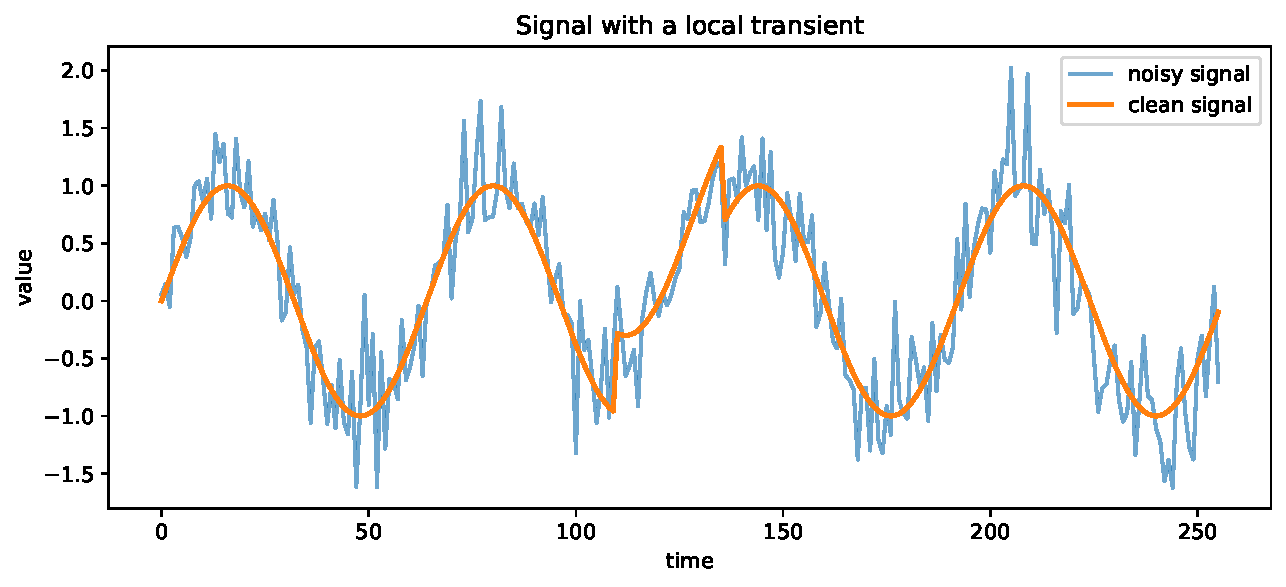
\includegraphics[keepaspectratio]{chapters/chapter-14-filtering-wavelets_files/figure-pdf/ch14-haar-transform-from-scratch-output-2.pdf}}

}

\caption{A Haar wavelet transform separates a signal into coarse and
detail coefficients.}

\end{figure}%

\begin{Shaded}
\begin{Highlighting}[]
\NormalTok{plt.figure(figsize}\OperatorTok{=}\NormalTok{(}\DecValTok{10}\NormalTok{, }\DecValTok{4}\NormalTok{))}
\ControlFlowTok{for}\NormalTok{ level, detail }\KeywordTok{in} \BuiltInTok{enumerate}\NormalTok{(details[:}\DecValTok{5}\NormalTok{], start}\OperatorTok{=}\DecValTok{1}\NormalTok{):}
    \CommentTok{\# Spread coefficients over the original time axis for visualization.}
\NormalTok{    centers }\OperatorTok{=}\NormalTok{ np.linspace(}\DecValTok{0}\NormalTok{, n }\OperatorTok{{-}} \DecValTok{1}\NormalTok{, }\BuiltInTok{len}\NormalTok{(detail), endpoint}\OperatorTok{=}\VariableTok{True}\NormalTok{)}
\NormalTok{    plt.plot(centers, detail }\OperatorTok{+} \FloatTok{2.5} \OperatorTok{*}\NormalTok{ (level }\OperatorTok{{-}} \DecValTok{1}\NormalTok{), marker}\OperatorTok{=}\StringTok{"o"}\NormalTok{, markersize}\OperatorTok{=}\DecValTok{2}\NormalTok{, linewidth}\OperatorTok{=}\DecValTok{1}\NormalTok{,}
\NormalTok{             label}\OperatorTok{=}\SpecialStringTok{f"detail level }\SpecialCharTok{\{}\NormalTok{level}\SpecialCharTok{\}}\SpecialStringTok{"}\NormalTok{)}
\NormalTok{plt.xlabel(}\StringTok{"time location"}\NormalTok{)}
\NormalTok{plt.ylabel(}\StringTok{"coefficient value plus vertical offset"}\NormalTok{)}
\NormalTok{plt.title(}\StringTok{"Multiscale Haar detail coefficients"}\NormalTok{)}
\NormalTok{plt.legend(ncol}\OperatorTok{=}\DecValTok{2}\NormalTok{)}
\NormalTok{plt.show()}
\end{Highlighting}
\end{Shaded}

\begin{figure}[H]

{\centering \pandocbounded{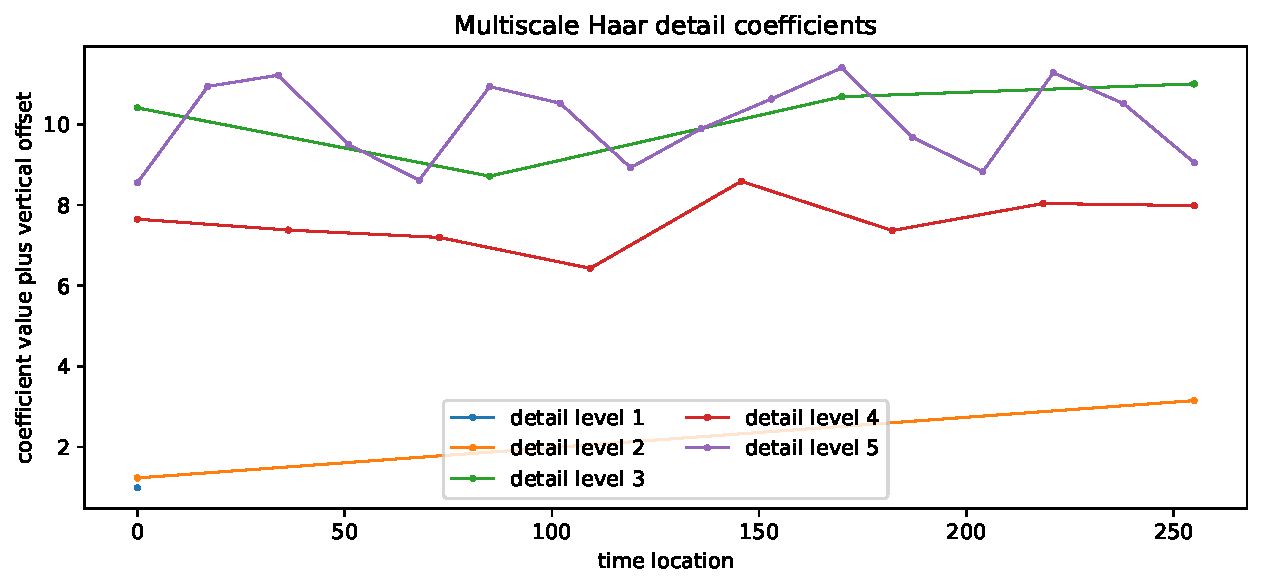
\includegraphics[keepaspectratio]{chapters/chapter-14-filtering-wavelets_files/figure-pdf/ch14-haar-detail-coefficients-output-1.pdf}}

}

\caption{Haar detail coefficients reveal local changes at different
scales.}

\end{figure}%

\section{14.13 Wavelet denoising}\label{wavelet-denoising}

Wavelet denoising is based on a simple observation. For many signals,
meaningful structure is represented by a relatively small number of
large wavelet coefficients, while noise is spread across many small
coefficients.

A common procedure is:

\begin{enumerate}
\def\labelenumi{\arabic{enumi}.}
\tightlist
\item
  compute wavelet coefficients;
\item
  estimate the noise level;
\item
  shrink or remove small detail coefficients;
\item
  invert the wavelet transform.
\end{enumerate}

A standard universal threshold is

\[
\lambda=\widehat\sigma\sqrt{2\log n}.
\]

A robust estimate of \(\sigma\) from the finest-scale detail
coefficients is

\[
\widehat\sigma=\frac{\operatorname{median}(|d_{J,k}|)}{0.6745}.
\]

Hard thresholding uses

\[
\eta_\lambda(d)=
\begin{cases}
d, & |d|>\lambda,\\
0, & |d|\leq \lambda.
\end{cases}
\]

Soft thresholding uses

\[
\eta_\lambda(d)=\operatorname{sign}(d)(|d|-\lambda)_+.
\]

Soft thresholding is continuous and often produces smoother
reconstructions.

\begin{Shaded}
\begin{Highlighting}[]
\KeywordTok{def}\NormalTok{ soft\_threshold(x, lam):}
    \ControlFlowTok{return}\NormalTok{ np.sign(x) }\OperatorTok{*}\NormalTok{ np.maximum(np.}\BuiltInTok{abs}\NormalTok{(x) }\OperatorTok{{-}}\NormalTok{ lam, }\FloatTok{0.0}\NormalTok{)}

\NormalTok{coarse, details }\OperatorTok{=}\NormalTok{ haar\_transform(noisy)}
\NormalTok{sigma\_hat }\OperatorTok{=}\NormalTok{ np.median(np.}\BuiltInTok{abs}\NormalTok{(details[}\OperatorTok{{-}}\DecValTok{1}\NormalTok{])) }\OperatorTok{/} \FloatTok{0.6745}
\NormalTok{lam }\OperatorTok{=}\NormalTok{ sigma\_hat }\OperatorTok{*}\NormalTok{ np.sqrt(}\DecValTok{2} \OperatorTok{*}\NormalTok{ np.log(n))}

\NormalTok{details\_soft }\OperatorTok{=}\NormalTok{ [soft\_threshold(d, lam) }\ControlFlowTok{for}\NormalTok{ d }\KeywordTok{in}\NormalTok{ details]}
\NormalTok{denoised }\OperatorTok{=}\NormalTok{ inverse\_haar\_transform(coarse, details\_soft)}

\NormalTok{plt.figure(figsize}\OperatorTok{=}\NormalTok{(}\DecValTok{10}\NormalTok{, }\DecValTok{4}\NormalTok{))}
\NormalTok{plt.plot(t, noisy, label}\OperatorTok{=}\StringTok{"noisy"}\NormalTok{, alpha}\OperatorTok{=}\FloatTok{0.45}\NormalTok{)}
\NormalTok{plt.plot(t, clean, label}\OperatorTok{=}\StringTok{"clean"}\NormalTok{, linewidth}\OperatorTok{=}\DecValTok{2}\NormalTok{)}
\NormalTok{plt.plot(t, denoised, label}\OperatorTok{=}\StringTok{"wavelet denoised"}\NormalTok{, linewidth}\OperatorTok{=}\DecValTok{2}\NormalTok{)}
\NormalTok{plt.xlabel(}\StringTok{"time"}\NormalTok{)}
\NormalTok{plt.ylabel(}\StringTok{"value"}\NormalTok{)}
\NormalTok{plt.title(}\StringTok{"Wavelet denoising with soft thresholding"}\NormalTok{)}
\NormalTok{plt.legend()}
\NormalTok{plt.show()}

\BuiltInTok{print}\NormalTok{(}\StringTok{"Noise estimate:"}\NormalTok{, sigma\_hat)}
\BuiltInTok{print}\NormalTok{(}\StringTok{"Universal threshold:"}\NormalTok{, lam)}
\BuiltInTok{print}\NormalTok{(}\StringTok{"RMSE noisy:"}\NormalTok{, np.sqrt(np.mean((noisy }\OperatorTok{{-}}\NormalTok{ clean) }\OperatorTok{**} \DecValTok{2}\NormalTok{)))}
\BuiltInTok{print}\NormalTok{(}\StringTok{"RMSE denoised:"}\NormalTok{, np.sqrt(np.mean((denoised }\OperatorTok{{-}}\NormalTok{ clean) }\OperatorTok{**} \DecValTok{2}\NormalTok{)))}
\end{Highlighting}
\end{Shaded}

\begin{figure}[H]

{\centering \pandocbounded{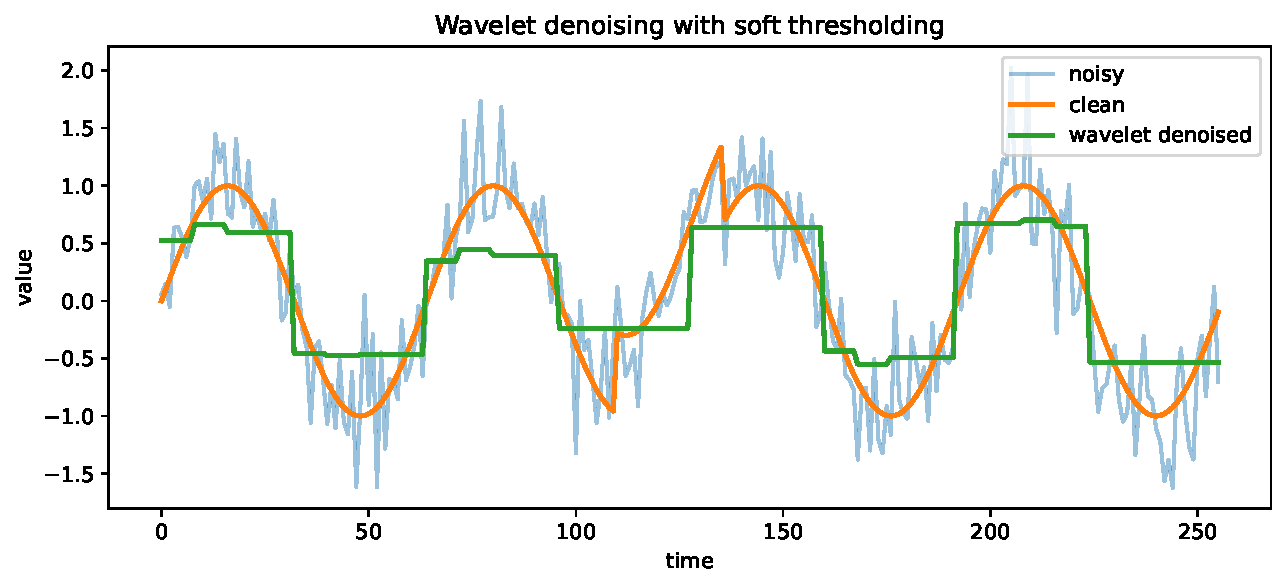
\includegraphics[keepaspectratio]{chapters/chapter-14-filtering-wavelets_files/figure-pdf/ch14-wavelet-denoising-output-1.pdf}}

}

\caption{Wavelet thresholding removes small coefficients and
reconstructs a denoised signal.}

\end{figure}%

\begin{verbatim}
Noise estimate: 0.35405931975368604
Universal threshold: 1.179094877137156
RMSE noisy: 0.3440840607572144
RMSE denoised: 0.3382220081869893
\end{verbatim}

\begin{tcolorbox}[enhanced jigsaw, arc=.35mm, bottomrule=.15mm, bottomtitle=1mm, breakable, colback=white, colbacktitle=quarto-callout-warning-color!10!white, colframe=quarto-callout-warning-color-frame, coltitle=black, left=2mm, leftrule=.75mm, opacityback=0, opacitybacktitle=0.6, rightrule=.15mm, title=\textcolor{quarto-callout-warning-color}{\faExclamationTriangle}\hspace{0.5em}{Denoising is not always forecasting improvement}, titlerule=0mm, toprule=.15mm, toptitle=1mm]

A denoised curve may look better but forecast worse if the threshold
removes predictive short-term variation. Always compare filtered and
unfiltered pipelines using time-aware validation.

\end{tcolorbox}

\section{14.14 Interactive HTML: Haar details and
denoising}\label{interactive-html-haar-details-and-denoising}

This module simulates a smooth signal with a local jump. A Haar
transform reacts strongly near abrupt changes. Increase the threshold to
remove small details and keep only larger local features.

\subsection{Interactive Haar denoising
explorer}\label{interactive-haar-denoising-explorer}

Noise level
\protect\phantomsection\label{ch14-wavelet-noise-value}{0.35} Threshold
\protect\phantomsection\label{ch14-wavelet-threshold-value}{0.45}

\protect\phantomsection\label{ch14-haar-signal-plot}

\protect\phantomsection\label{ch14-haar-detail-plot}

\section{14.15 Wavelets as features for machine
learning}\label{wavelets-as-features-for-machine-learning}

Wavelet transforms are not only visualization tools. They can be used to
construct features for supervised or unsupervised learning.

For a time window \(x_{t-L+1:t}\), possible wavelet features include:

\begin{itemize}
\tightlist
\item
  energy at each scale;
\item
  maximum absolute detail coefficient at each scale;
\item
  number of coefficients exceeding a threshold;
\item
  entropy of normalized wavelet energy;
\item
  scale where the largest event occurs;
\item
  reconstructed low-frequency trend;
\item
  reconstructed high-frequency residual.
\end{itemize}

These features are useful for:

\begin{itemize}
\tightlist
\item
  anomaly detection in sensors;
\item
  classification of ECG or EEG segments;
\item
  machine-health monitoring;
\item
  event detection in audio and seismic data;
\item
  multiscale forecasting features for tree-based models.
\end{itemize}

A scale-energy feature is

\[
E_j=\sum_k d_{j,k}^2,
\]

where \(d_{j,k}\) is the detail coefficient at scale \(j\) and location
\(k\).

The normalized energy distribution is

\[
p_j=\frac{E_j}{\sum_\ell E_\ell}.
\]

A wavelet entropy feature is

\[
H=-\sum_j p_j\log p_j.
\]

Low entropy means the signal's variation is concentrated at a few
scales. High entropy means variation is spread over many scales.

\begin{Shaded}
\begin{Highlighting}[]
\NormalTok{coarse, details }\OperatorTok{=}\NormalTok{ haar\_transform(noisy)}
\NormalTok{scale\_energies }\OperatorTok{=}\NormalTok{ np.array([np.}\BuiltInTok{sum}\NormalTok{(d }\OperatorTok{**} \DecValTok{2}\NormalTok{) }\ControlFlowTok{for}\NormalTok{ d }\KeywordTok{in}\NormalTok{ details])}
\NormalTok{p }\OperatorTok{=}\NormalTok{ scale\_energies }\OperatorTok{/}\NormalTok{ scale\_energies.}\BuiltInTok{sum}\NormalTok{()}
\NormalTok{entropy }\OperatorTok{=} \OperatorTok{{-}}\NormalTok{np.}\BuiltInTok{sum}\NormalTok{(p }\OperatorTok{*}\NormalTok{ np.log(p }\OperatorTok{+} \FloatTok{1e{-}12}\NormalTok{))}

\NormalTok{plt.figure(figsize}\OperatorTok{=}\NormalTok{(}\DecValTok{8}\NormalTok{, }\DecValTok{4}\NormalTok{))}
\NormalTok{plt.bar(np.arange(}\DecValTok{1}\NormalTok{, }\BuiltInTok{len}\NormalTok{(scale\_energies) }\OperatorTok{+} \DecValTok{1}\NormalTok{), scale\_energies)}
\NormalTok{plt.xlabel(}\StringTok{"detail scale"}\NormalTok{)}
\NormalTok{plt.ylabel(}\StringTok{"energy"}\NormalTok{)}
\NormalTok{plt.title(}\SpecialStringTok{f"Wavelet scale energies; entropy = }\SpecialCharTok{\{}\NormalTok{entropy}\SpecialCharTok{:.3f\}}\SpecialStringTok{"}\NormalTok{)}
\NormalTok{plt.show()}
\end{Highlighting}
\end{Shaded}

\begin{figure}[H]

{\centering \pandocbounded{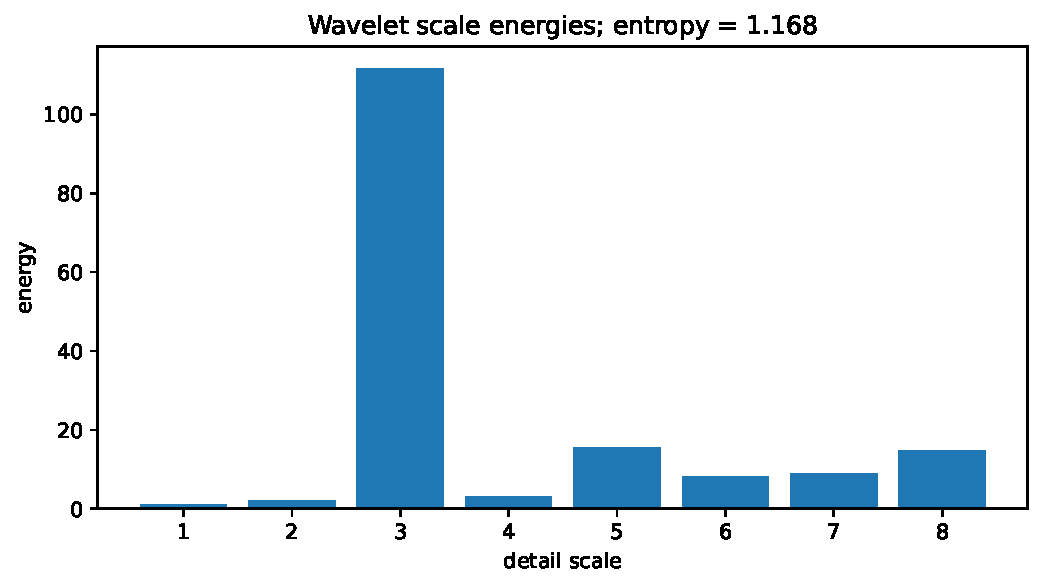
\includegraphics[keepaspectratio]{chapters/chapter-14-filtering-wavelets_files/figure-pdf/ch14-wavelet-features-output-1.pdf}}

}

\caption{Wavelet scale energies summarize multiscale structure.}

\end{figure}%

\section{14.16 Mini case study: detecting a transient
burst}\label{mini-case-study-detecting-a-transient-burst}

The following example compares global Fourier evidence with local
wavelet evidence. A short high-frequency burst may not dominate the
global periodogram, but it can produce large local detail coefficients.

\protect\phantomsection\label{ch14-transient-burst-case-study}
\begin{Shaded}
\begin{Highlighting}[]
\NormalTok{n }\OperatorTok{=} \DecValTok{512}
\NormalTok{t }\OperatorTok{=}\NormalTok{ np.arange(n)}
\NormalTok{base }\OperatorTok{=}\NormalTok{ np.sin(}\DecValTok{2} \OperatorTok{*}\NormalTok{ np.pi }\OperatorTok{*}\NormalTok{ t }\OperatorTok{/} \DecValTok{80}\NormalTok{)}
\NormalTok{burst }\OperatorTok{=}\NormalTok{ np.zeros(n)}
\NormalTok{burst\_window }\OperatorTok{=}\NormalTok{ (t }\OperatorTok{\textgreater{}=} \DecValTok{240}\NormalTok{) }\OperatorTok{\&}\NormalTok{ (t }\OperatorTok{\textless{}=} \DecValTok{300}\NormalTok{)}
\NormalTok{burst[burst\_window] }\OperatorTok{=} \FloatTok{0.8} \OperatorTok{*}\NormalTok{ np.sin(}\DecValTok{2} \OperatorTok{*}\NormalTok{ np.pi }\OperatorTok{*} \FloatTok{0.28} \OperatorTok{*}\NormalTok{ t[burst\_window])}
\NormalTok{x\_burst }\OperatorTok{=}\NormalTok{ base }\OperatorTok{+}\NormalTok{ burst }\OperatorTok{+} \FloatTok{0.25} \OperatorTok{*}\NormalTok{ rng.normal(size}\OperatorTok{=}\NormalTok{n)}

\CommentTok{\# Periodogram}
\NormalTok{x\_centered }\OperatorTok{=}\NormalTok{ x\_burst }\OperatorTok{{-}}\NormalTok{ x\_burst.mean()}
\NormalTok{D }\OperatorTok{=}\NormalTok{ np.fft.rfft(x\_centered)}
\NormalTok{freq }\OperatorTok{=}\NormalTok{ np.fft.rfftfreq(n, d}\OperatorTok{=}\DecValTok{1}\NormalTok{)}
\NormalTok{I }\OperatorTok{=}\NormalTok{ (np.}\BuiltInTok{abs}\NormalTok{(D) }\OperatorTok{**} \DecValTok{2}\NormalTok{) }\OperatorTok{/}\NormalTok{ n}

\NormalTok{coarse\_b, details\_b }\OperatorTok{=}\NormalTok{ haar\_transform(x\_burst)}
\CommentTok{\# Use a fine{-}to{-}medium detail level for transient detection.}
\NormalTok{detail }\OperatorTok{=}\NormalTok{ details\_b[}\OperatorTok{{-}}\DecValTok{2}\NormalTok{]}
\NormalTok{loc }\OperatorTok{=}\NormalTok{ np.linspace(}\DecValTok{0}\NormalTok{, n }\OperatorTok{{-}} \DecValTok{1}\NormalTok{, }\BuiltInTok{len}\NormalTok{(detail), endpoint}\OperatorTok{=}\VariableTok{True}\NormalTok{)}

\NormalTok{plt.figure(figsize}\OperatorTok{=}\NormalTok{(}\DecValTok{10}\NormalTok{, }\DecValTok{3}\NormalTok{))}
\NormalTok{plt.plot(t, x\_burst)}
\NormalTok{plt.axvspan(}\DecValTok{240}\NormalTok{, }\DecValTok{300}\NormalTok{, alpha}\OperatorTok{=}\FloatTok{0.2}\NormalTok{, label}\OperatorTok{=}\StringTok{"true burst interval"}\NormalTok{)}
\NormalTok{plt.xlabel(}\StringTok{"time"}\NormalTok{)}
\NormalTok{plt.ylabel(}\StringTok{"value"}\NormalTok{)}
\NormalTok{plt.title(}\StringTok{"Signal with a local high{-}frequency burst"}\NormalTok{)}
\NormalTok{plt.legend()}
\NormalTok{plt.show()}

\NormalTok{plt.figure(figsize}\OperatorTok{=}\NormalTok{(}\DecValTok{8}\NormalTok{, }\DecValTok{3}\NormalTok{))}
\NormalTok{plt.plot(freq, I)}
\NormalTok{plt.xlabel(}\StringTok{"frequency"}\NormalTok{)}
\NormalTok{plt.ylabel(}\StringTok{"periodogram"}\NormalTok{)}
\NormalTok{plt.title(}\StringTok{"Global periodogram"}\NormalTok{)}
\NormalTok{plt.show()}

\NormalTok{plt.figure(figsize}\OperatorTok{=}\NormalTok{(}\DecValTok{10}\NormalTok{, }\DecValTok{3}\NormalTok{))}
\NormalTok{plt.plot(loc, np.}\BuiltInTok{abs}\NormalTok{(detail), marker}\OperatorTok{=}\StringTok{"o"}\NormalTok{, markersize}\OperatorTok{=}\DecValTok{2}\NormalTok{)}
\NormalTok{plt.axvspan(}\DecValTok{240}\NormalTok{, }\DecValTok{300}\NormalTok{, alpha}\OperatorTok{=}\FloatTok{0.2}\NormalTok{, label}\OperatorTok{=}\StringTok{"true burst interval"}\NormalTok{)}
\NormalTok{plt.xlabel(}\StringTok{"time location"}\NormalTok{)}
\NormalTok{plt.ylabel(}\StringTok{"absolute detail coefficient"}\NormalTok{)}
\NormalTok{plt.title(}\StringTok{"Local wavelet detail response"}\NormalTok{)}
\NormalTok{plt.legend()}
\NormalTok{plt.show()}
\end{Highlighting}
\end{Shaded}

\begin{figure}[H]

{\centering \pandocbounded{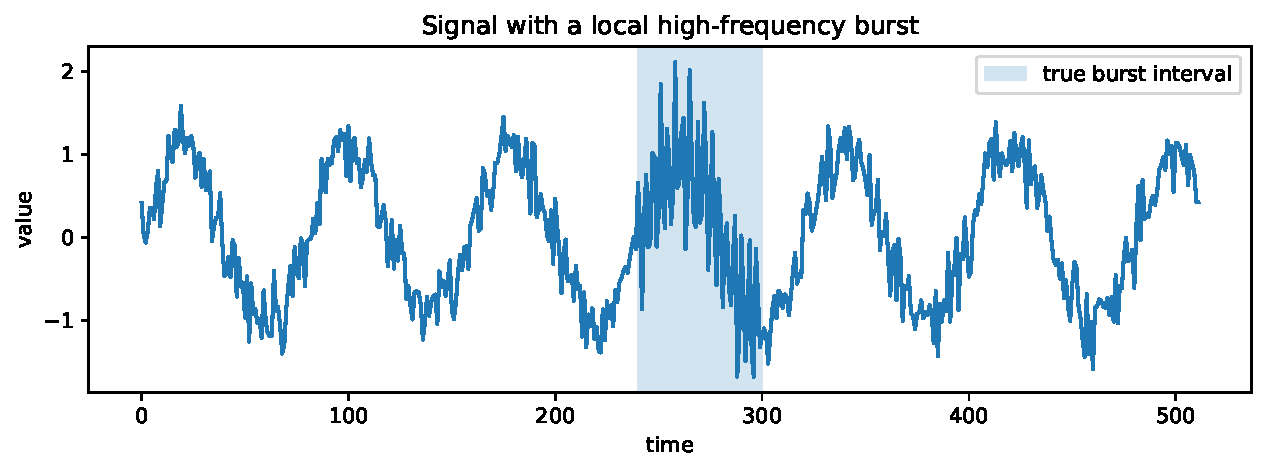
\includegraphics[keepaspectratio]{chapters/chapter-14-filtering-wavelets_files/figure-pdf/ch14-transient-burst-case-study-output-1.pdf}}

}

\caption{A local burst is easier to locate with wavelet details than
with a global spectrum.}

\end{figure}%

\pandocbounded{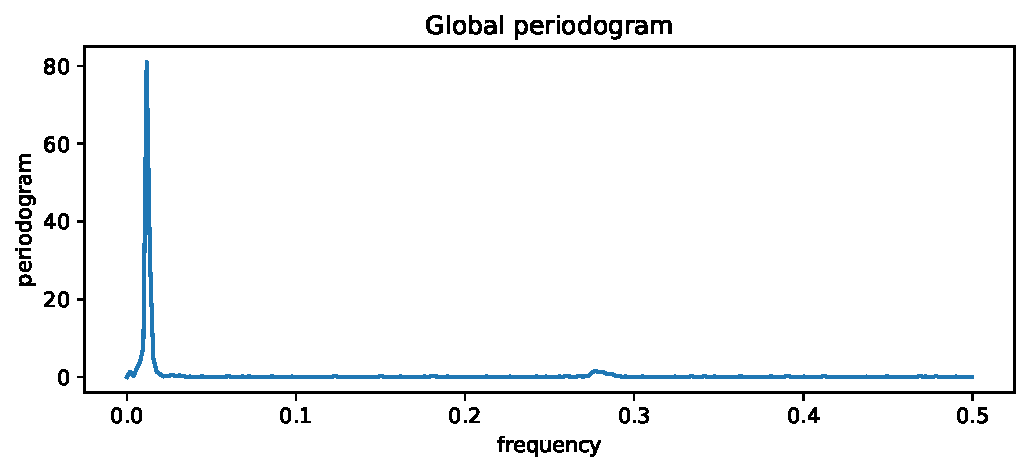
\includegraphics[keepaspectratio]{chapters/chapter-14-filtering-wavelets_files/figure-pdf/ch14-transient-burst-case-study-output-2.pdf}}

\pandocbounded{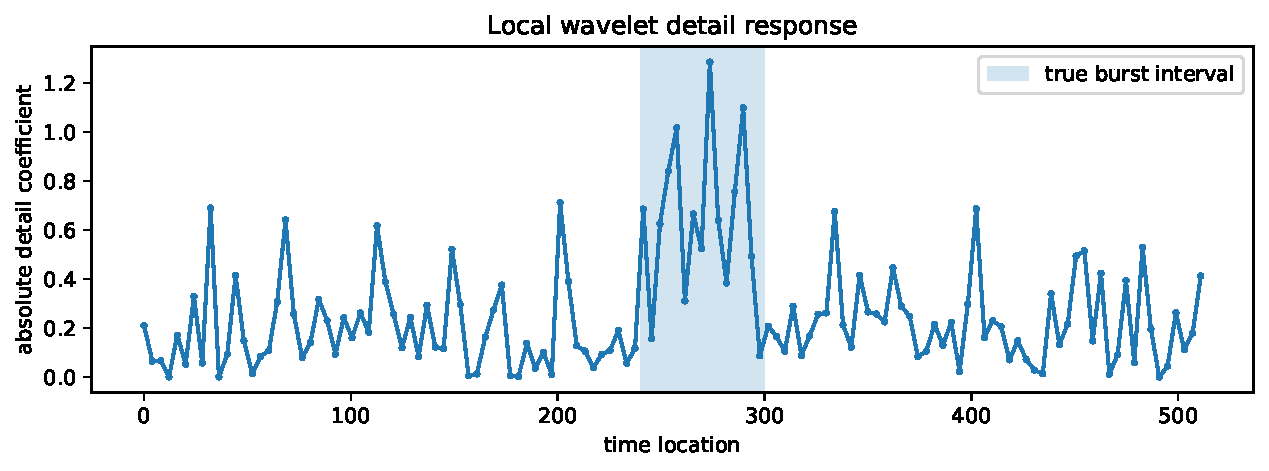
\includegraphics[keepaspectratio]{chapters/chapter-14-filtering-wavelets_files/figure-pdf/ch14-transient-burst-case-study-output-3.pdf}}

\section{14.17 AI-assisted modeling box}\label{ai-assisted-modeling-box}

\section{Using AI to critique filtering and
wavelets}\label{using-ai-to-critique-filtering-and-wavelets}

Ask an AI assistant questions like these, then verify the answers
mathematically and computationally.

\textbf{Prompt 1. Filtering choice}

\begin{quote}
I have a daily time series with weekly seasonality, long-term trend, and
occasional spikes. I want to forecast 14 days ahead. Should I use a
centered moving average, trailing moving average, differencing, or
wavelet denoising? State the leakage risk for each option.
\end{quote}

\textbf{Prompt 2. Frequency response}

\begin{quote}
Derive the frequency response of the filter \(Y_t=X_t-X_{t-7}\). Which
frequencies are removed? Explain in terms of the squared gain.
\end{quote}

\textbf{Prompt 3. Wavelet interpretation}

\begin{quote}
A signal has high wavelet detail energy at fine scales only during a
short time interval. Give three possible explanations and one diagnostic
plot for each.
\end{quote}

\textbf{Prompt 4. ML feature design}

\begin{quote}
Build leakage-safe wavelet features for a rolling forecasting model. The
features must use only information available up to forecast origin
\(t\).
\end{quote}

Verification checklist:

\begin{enumerate}
\def\labelenumi{\arabic{enumi}.}
\tightlist
\item
  Did the AI distinguish exploratory smoothing from forecasting
  features?
\item
  Did it state whether the filter is causal?
\item
  Did it derive or at least correctly describe \(|A(\omega)|^2\)?
\item
  Did it mention that denoising can remove predictive signal?
\item
  Did it propose time-aware validation rather than random splitting?
\end{enumerate}

\section{14.18 Common mistakes}\label{common-mistakes-13}

\begin{enumerate}
\def\labelenumi{\arabic{enumi}.}
\item
  \textbf{Using centered filters for forecasting features.}\\
  This leaks future observations into the training data.
\item
  \textbf{Assuming smoothing always improves forecasting.}\\
  Smoothing can remove short-term signals that are useful for
  prediction.
\item
  \textbf{Interpreting filter output without understanding the frequency
  response.}\\
  Always ask which frequencies were amplified and which were suppressed.
\item
  \textbf{Treating wavelet coefficients as magic anomaly scores.}\\
  Large coefficients may indicate jumps, bursts, edges, noise, or
  boundary artifacts.
\item
  \textbf{Ignoring boundary effects.}\\
  Convolution and wavelet transforms need conventions near the beginning
  and end of the sample.
\item
  \textbf{Comparing filtered and unfiltered models on different
  validation schemes.}\\
  Use the same rolling-origin evaluation design.
\item
  \textbf{Forgetting scale.}\\
  A wavelet coefficient is meaningful only relative to its scale, noise
  level, and boundary position.
\end{enumerate}

\section{14.19 Exercises}\label{exercises-13}

\begin{enumerate}
\def\labelenumi{\arabic{enumi}.}
\item
  \textbf{Frequency response of a difference filter.}\\
  Derive the frequency response and squared gain of \(Y_t=X_t-X_{t-1}\).
  Explain why it removes low-frequency components.
\item
  \textbf{Seasonal difference.}\\
  For \(Y_t=X_t-X_{t-s}\), show that \[
  |A(\omega)|^2=4\sin^2(\pi s\omega).
  \] Which frequencies are removed?
\item
  \textbf{Moving average response.}\\
  Derive the frequency response of the trailing moving average \[
  Y_t=\frac{1}{m}\sum_{j=0}^{m-1}X_{t-j}.
  \] Use Python to plot \(|A(\omega)|^2\) for \(m=5,13,25\).
\item
  \textbf{Filtering white noise.}\\
  Let \(X_t\sim WN(0,\sigma^2)\) and \(Y_t=(X_t+X_{t-1})/2\). Compute
  \(\gamma_Y(0)\) and \(\gamma_Y(1)\). Then verify by simulation.
\item
  \textbf{Leakage diagnosis.}\\
  A student uses \(Z_t=(X_{t-2}+X_{t-1}+X_t+X_{t+1}+X_{t+2})/5\) as a
  feature to predict \(X_{t+1}\). Identify the leakage and propose a
  corrected feature.
\item
  \textbf{Haar transform by hand.}\\
  Compute the Haar coefficients of \((4,6,10,14)\) using the orthonormal
  averaging/detail convention.
\item
  \textbf{Energy preservation.}\\
  Prove that the two-point Haar transform preserves squared norm: \[
  x_0^2+x_1^2=a^2+d^2.
  \]
\item
  \textbf{Wavelet denoising experiment.}\\
  Simulate a piecewise-constant signal plus Gaussian noise. Apply Haar
  soft thresholding. Compare RMSE before and after denoising.
\item
  \textbf{Transient detection.}\\
  Simulate a sinusoid with a short burst. Compare a global periodogram
  with wavelet detail coefficients. Which method locates the burst more
  clearly?
\item
  \textbf{AI verification.}\\
  Ask an AI assistant to recommend a filter for a seasonal forecasting
  problem. Write a critique of its recommendation using causality,
  frequency response, and validation design.
\end{enumerate}

\section{14.20 Mini project}\label{mini-project}

Choose a real or simulated time series with at least one of the
following properties:

\begin{itemize}
\tightlist
\item
  trend plus high-frequency noise;
\item
  seasonal pattern plus spikes;
\item
  transient burst;
\item
  changing frequency over time;
\item
  sensor signal with anomalies.
\end{itemize}

Your report should include:

\begin{enumerate}
\def\labelenumi{\arabic{enumi}.}
\tightlist
\item
  a raw time plot;
\item
  at least two filters and their frequency responses;
\item
  a comparison of filtered and unfiltered periodograms;
\item
  a Haar or wavelet-style multiresolution analysis;
\item
  a leakage-safe statement explaining whether each filter can be used
  for forecasting;
\item
  a short AI-assisted modeling log, including one AI suggestion you
  accepted and one you rejected;
\item
  a final recommendation: smoothing, differencing, wavelet features, or
  no filtering.
\end{enumerate}

\section{14.21 Chapter checklist}\label{chapter-checklist-11}

By the end of this chapter, you should be able to say:

\begin{itemize}
\tightlist
\item
  I can write a linear filter as \(Y_t=\sum_j a_jX_{t-j}\).
\item
  I can compute a filter's frequency response \(A(\omega)\).
\item
  I can explain why filtering changes spectral density by
  \(|A(\omega)|^2\).
\item
  I can distinguish low-pass, high-pass, and seasonal-difference
  filters.
\item
  I can identify leakage caused by noncausal smoothing.
\item
  I can explain why Fourier methods are global.
\item
  I can describe the purpose of wavelets in time-frequency localization.
\item
  I can implement a basic Haar transform from scratch.
\item
  I can use wavelet coefficients for denoising or transient detection.
\item
  I can evaluate filtering choices with time-aware validation.
\end{itemize}

\section{14.22 Further reading}\label{further-reading-3}

\begin{itemize}
\tightlist
\item
  Shumway and Stoffer, \emph{Time Series Analysis and Its Applications},
  sections on filters and spectral analysis.
\item
  Percival and Walden, \emph{Wavelet Methods for Time Series Analysis}.
\item
  Mallat, \emph{A Wavelet Tour of Signal Processing}.
\item
  Strang and Nguyen, \emph{Wavelets and Filter Banks}.
\item
  Brockwell and Davis, \emph{Introduction to Time Series and
  Forecasting}, chapters on linear filters and spectral methods.
\end{itemize}

\part{Part V. Forecasting at Scale and Machine Learning Methods}

\chapter{Forecast Evaluation and
Backtesting}\label{forecast-evaluation-and-backtesting}

\textbf{Part V. Forecasting at Scale and Machine Learning Methods}\\
\textbf{Chapter goal:} learn how to evaluate forecasts as time-indexed
decisions rather than ordinary predictions on randomly shuffled data. We
develop point-forecast metrics, horizon-wise errors, rolling-origin
backtesting, leakage checks, baseline models, and uncertainty-aware
evaluation.

\section{Learning objectives}\label{learning-objectives-14}

After studying this chapter, you should be able to:

\begin{enumerate}
\def\labelenumi{\arabic{enumi}.}
\tightlist
\item
  define forecast origin, forecast horizon, point forecast, prediction
  interval, and forecast error;
\item
  explain why random train-test splits are usually invalid for time
  series;
\item
  implement holdout, expanding-window, sliding-window, and
  rolling-origin backtests;
\item
  compute MAE, RMSE, MAPE, sMAPE, MASE, RMSSE, bias, coverage, and
  interval width;
\item
  compare models horizon by horizon rather than only through a single
  average score;
\item
  construct naive, seasonal naive, drift, and moving-average baselines;
\item
  diagnose leakage from future variables, centered smoothers, scaling,
  target transformations, and feature engineering;
\item
  distinguish residual diagnostics from out-of-sample forecast
  evaluation;
\item
  evaluate probabilistic forecasts using interval coverage and quantile
  loss;
\item
  use AI tools to critique evaluation designs, but verify the design
  mathematically and computationally.
\end{enumerate}

\section{15.1 Why forecast evaluation is a separate
topic}\label{why-forecast-evaluation-is-a-separate-topic}

A model can have beautiful mathematics and still fail as a forecasting
tool. Conversely, a simple baseline can be very hard to beat when the
data contain strong persistence or seasonality. Forecast evaluation
asks:

\begin{quote}
If we had used this model in the past, how well would it have predicted
the future that was not yet observed?
\end{quote}

This is different from asking whether a model fits historical data. The
distinction is central in time-series analysis because observations are
ordered. A model trained using information from time \(t+1\) should not
be evaluated as if it had been available at time \(t\).

In the ARIMA and SARIMA workflow from earlier chapters, model building
includes exploratory analysis, parameter estimation, residual
diagnostics, and model selection. The notes emphasize residual ACF,
Ljung--Box testing, and forecast comparison as part of the modeling
loop. This chapter makes the forecast-comparison step explicit and
prepares for automated forecasting, Prophet-type models,
machine-learning features, and deep-learning models.

\begin{tcolorbox}[enhanced jigsaw, arc=.35mm, bottomrule=.15mm, bottomtitle=1mm, breakable, colback=white, colbacktitle=quarto-callout-note-color!10!white, colframe=quarto-callout-note-color-frame, coltitle=black, left=2mm, leftrule=.75mm, opacityback=0, opacitybacktitle=0.6, rightrule=.15mm, title=\textcolor{quarto-callout-note-color}{\faInfo}\hspace{0.5em}{Model fit is not forecast accuracy}, titlerule=0mm, toprule=.15mm, toptitle=1mm]

A model with small in-sample residuals can forecast poorly. Forecast
evaluation must mimic the information structure of the real forecasting
task.

\end{tcolorbox}

\section{15.2 Forecast notation}\label{forecast-notation}

Let \(\{Y_t\}_{t=1}^T\) be an observed time series. At time \(t\), the
information available to a forecaster is denoted by

\[
\mathcal F_t=\sigma(Y_t,Y_{t-1},\ldots),
\]

or, in applied work, by the data table available at forecast origin
\(t\).

A forecast for \(h\) periods ahead made at time \(t\) is written

\[
\widehat Y_{t+h\mid t}.
\]

Here:

\begin{itemize}
\tightlist
\item
  \(t\) is the \textbf{forecast origin};
\item
  \(h\) is the \textbf{forecast horizon};
\item
  \(Y_{t+h}\) is the future value eventually observed;
\item
  \(\widehat Y_{t+h\mid t}\) is the forecast made without seeing
  \(Y_{t+h}\).
\end{itemize}

The forecast error is

\[
e_{t,h}=Y_{t+h}-\widehat Y_{t+h\mid t}.
\]

For a set of forecast origins \(\mathcal T_h\), an empirical
horizon-\(h\) risk under loss \(L\) is

\[
\widehat R_h
=\frac{1}{|\mathcal T_h|}
\sum_{t\in\mathcal T_h}L(Y_{t+h},\widehat Y_{t+h\mid t}).
\]

For example, squared-error loss is

\[
L(y,\hat y)=(y-\hat y)^2,
\]

and absolute-error loss is

\[
L(y,\hat y)=|y-\hat y|.
\]

A complete evaluation often reports \(\widehat R_h\) for each horizon
\(h=1,\ldots,H\), not only the average

\[
\widehat R_{1:H}
=\frac{1}{H}\sum_{h=1}^H\widehat R_h.
\]

\begin{tcolorbox}[enhanced jigsaw, arc=.35mm, bottomrule=.15mm, bottomtitle=1mm, breakable, colback=white, colbacktitle=quarto-callout-tip-color!10!white, colframe=quarto-callout-tip-color-frame, coltitle=black, left=2mm, leftrule=.75mm, opacityback=0, opacitybacktitle=0.6, rightrule=.15mm, title=\textcolor{quarto-callout-tip-color}{\faLightbulb}\hspace{0.5em}{Horizon matters}, titlerule=0mm, toprule=.15mm, toptitle=1mm]

A model may be excellent one step ahead but poor twelve steps ahead.
Report scores by horizon whenever the application cares about more than
one lead time.

\end{tcolorbox}

\section{15.3 Proper time-aware train/test
splits}\label{proper-time-aware-traintest-splits}

In ordinary supervised learning, we often split rows randomly. For time
series, random splitting usually leaks future information into the past.
A time-aware split preserves order.

Suppose the observations are

\[
Y_1,Y_2,\ldots,Y_T.
\]

A simple holdout split chooses a cutoff \(T_0<T\):

\[
\text{train}=\{1,\ldots,T_0\},
\qquad
\text{test}=\{T_0+1,\ldots,T\}.
\]

This is useful but can be unstable: one test period may be unusually
easy or hard. Backtesting creates many historical forecasting
experiments.

\subsection{Expanding-window
backtesting}\label{expanding-window-backtesting}

In an expanding-window backtest, the training set grows over time. For
forecast origin \(t\), the model is trained on

\[
Y_1,\ldots,Y_t
\]

and predicts

\[
Y_{t+1},Y_{t+2},\ldots,Y_{t+H}.
\]

The next origin uses one more observation. This matches settings where
all past data remain relevant.

\subsection{Sliding-window
backtesting}\label{sliding-window-backtesting}

In a sliding-window backtest with window length \(w\), the model at
origin \(t\) is trained on

\[
Y_{t-w+1},\ldots,Y_t.
\]

This is useful when the data-generating process changes over time and
old data may be less relevant.

\subsection{Fixed-origin holdout}\label{fixed-origin-holdout}

A fixed-origin test evaluates one final forecasting episode. It is easy
to explain, but it gives fewer forecast errors.

\subsection{Blocked cross-validation}\label{blocked-cross-validation}

Blocked cross-validation splits the series into contiguous blocks. It
can be useful for model selection when the goal is to estimate average
future performance, but the blocks must be designed carefully so that
future observations do not help predict earlier observations.

\begin{tcolorbox}[enhanced jigsaw, arc=.35mm, bottomrule=.15mm, bottomtitle=1mm, breakable, colback=white, colbacktitle=quarto-callout-warning-color!10!white, colframe=quarto-callout-warning-color-frame, coltitle=black, left=2mm, leftrule=.75mm, opacityback=0, opacitybacktitle=0.6, rightrule=.15mm, title=\textcolor{quarto-callout-warning-color}{\faExclamationTriangle}\hspace{0.5em}{Do not shuffle time}, titlerule=0mm, toprule=.15mm, toptitle=1mm]

Randomly shuffling time-series rows destroys the temporal order. It can
make a bad forecasting model look good by allowing future information to
appear in the training set.

\end{tcolorbox}

\section{15.4 Baseline forecasts}\label{baseline-forecasts}

A sophisticated model should beat simple baselines. Baselines also
reveal the structure of the problem.

\subsection{Mean forecast}\label{mean-forecast}

The mean forecast uses the training average:

\[
\widehat Y_{t+h\mid t}=\bar Y_t
=\frac{1}{t}\sum_{j=1}^tY_j.
\]

This is a reasonable baseline for stationary series with weak
dependence.

\subsection{Naive forecast}\label{naive-forecast}

The naive forecast uses the most recent value:

\[
\widehat Y_{t+h\mid t}=Y_t.
\]

It is strong for persistent processes, random walks, and many financial
prices.

\subsection{Seasonal naive forecast}\label{seasonal-naive-forecast}

If the period is \(s\), the seasonal naive forecast is

\[
\widehat Y_{t+h\mid t}=Y_{t+h-ks},
\]

where \(k\) is the smallest positive integer such that \(t+h-ks\le t\).
For a one-season-ahead forecast at matching seasonal position, this is
often written as

\[
\widehat Y_{t+h\mid t}=Y_{t+h-s}.
\]

This is a strong baseline for monthly, weekly, hourly, and daily
seasonal data.

\subsection{Drift forecast}\label{drift-forecast}

The drift forecast connects the first and last training observations by
a line:

\[
\widehat Y_{t+h\mid t}
=Y_t+h\frac{Y_t-Y_1}{t-1}.
\]

It is useful for trending data.

\subsection{Moving-average forecast}\label{moving-average-forecast}

A causal moving-average forecast uses only past values:

\[
\widehat Y_{t+h\mid t}
=\frac{1}{m}\sum_{j=0}^{m-1}Y_{t-j}.
\]

For forecasting, avoid centered moving averages because they use future
observations.

\section{15.5 Point forecast metrics}\label{point-forecast-metrics}

Let \(e_i=y_i-\hat y_i\) for forecast cases \(i=1,\ldots,n\).

\subsection{Mean error and bias}\label{mean-error-and-bias}

The mean error is

\[
\operatorname{ME}=\frac{1}{n}\sum_{i=1}^n e_i.
\]

A positive ME means the forecasts are too low on average, because
\(y_i-\hat y_i>0\).

Bias alone is not enough. A model can have zero mean error while making
large positive and negative mistakes.

\subsection{MAE}\label{mae}

The mean absolute error is

\[
\operatorname{MAE}=\frac{1}{n}\sum_{i=1}^n |e_i|.
\]

MAE is measured in the same units as the data and is robust relative to
squared-error metrics.

\subsection{MSE and RMSE}\label{mse-and-rmse}

The mean squared error is

\[
\operatorname{MSE}=\frac{1}{n}\sum_{i=1}^n e_i^2.
\]

The root mean squared error is

\[
\operatorname{RMSE}=\sqrt{\frac{1}{n}\sum_{i=1}^n e_i^2}.
\]

RMSE penalizes large errors more heavily than MAE.

\subsection{Percentage errors}\label{percentage-errors}

The mean absolute percentage error is

\[
\operatorname{MAPE}
=\frac{100}{n}\sum_{i=1}^n
\left|\frac{e_i}{y_i}\right|.
\]

MAPE is easy to communicate but can be unstable or undefined when
\(y_i\) is zero or close to zero.

The symmetric MAPE is

\[
\operatorname{sMAPE}
=\frac{100}{n}\sum_{i=1}^n
\frac{2|y_i-\hat y_i|}{|y_i|+|\hat y_i|}.
\]

Despite its name, sMAPE still has edge cases when both values are close
to zero.

\subsection{MASE}\label{mase}

The mean absolute scaled error compares a model to a naive benchmark.
For nonseasonal data, define the training-scale denominator

\[
Q_{\text{naive}}
=\frac{1}{T_{\text{train}}-1}
\sum_{t=2}^{T_{\text{train}}}|Y_t-Y_{t-1}|.
\]

Then

\[
\operatorname{MASE}
=\frac{\frac{1}{n}\sum_{i=1}^n|e_i|}{Q_{\text{naive}}}.
\]

For seasonal data with period \(s\), use

\[
Q_{\text{seasonal}}
=\frac{1}{T_{\text{train}}-s}
\sum_{t=s+1}^{T_{\text{train}}}|Y_t-Y_{t-s}|.
\]

A MASE below \(1\) means the model improves on the corresponding naive
forecast, using the training scale.

\subsection{RMSSE}\label{rmsse}

A squared-error version is

\[
\operatorname{RMSSE}
=
\sqrt{
\frac{
\frac{1}{n}\sum_{i=1}^n e_i^2
}{
\frac{1}{T_{\text{train}}-s}
\sum_{t=s+1}^{T_{\text{train}}}(Y_t-Y_{t-s})^2
}
}.
\]

This is useful when squared-error loss better matches the application.

\begin{tcolorbox}[enhanced jigsaw, arc=.35mm, bottomrule=.15mm, bottomtitle=1mm, breakable, colback=white, colbacktitle=quarto-callout-note-color!10!white, colframe=quarto-callout-note-color-frame, coltitle=black, left=2mm, leftrule=.75mm, opacityback=0, opacitybacktitle=0.6, rightrule=.15mm, title=\textcolor{quarto-callout-note-color}{\faInfo}\hspace{0.5em}{Choosing a metric}, titlerule=0mm, toprule=.15mm, toptitle=1mm]

Choose the metric before comparing models. Use MAE when absolute
mistakes matter, RMSE when large mistakes are especially costly,
MASE/RMSSE when comparing across series, and quantile loss when
evaluating prediction intervals or probabilistic forecasts.

\end{tcolorbox}

\section{15.6 Multi-horizon evaluation}\label{multi-horizon-evaluation}

For horizon \(h\), define

\[
e_{t,h}=Y_{t+h}-\widehat Y_{t+h\mid t}.
\]

Then horizon-specific MAE is

\[
\operatorname{MAE}_h
=\frac{1}{|\mathcal T_h|}
\sum_{t\in\mathcal T_h}|e_{t,h}|.
\]

A model may be selected by minimizing an average over horizons:

\[
\operatorname{MAE}_{1:H}
=\frac{1}{H}\sum_{h=1}^H\operatorname{MAE}_h,
\]

or by a weighted version

\[
\operatorname{WMAE}_{1:H}
=\sum_{h=1}^H w_h\operatorname{MAE}_h,
\qquad
\sum_{h=1}^H w_h=1.
\]

Weights should reflect the application. For inventory decisions,
near-term accuracy may be more important. For planning, longer horizons
may matter more.

\section{15.7 Direct, recursive, and multi-output
forecasting}\label{direct-recursive-and-multi-output-forecasting}

The evaluation design must match the forecasting strategy.

\subsection{Recursive strategy}\label{recursive-strategy}

A one-step model is iterated forward:

\[
\widehat Y_{t+2\mid t}
=f(\widehat Y_{t+1\mid t},Y_t,Y_{t-1},\ldots).
\]

Recursive forecasts can accumulate error.

\subsection{Direct strategy}\label{direct-strategy}

A separate model is trained for each horizon:

\[
\widehat Y_{t+h\mid t}=f_h(Y_t,Y_{t-1},\ldots).
\]

This avoids recursive error propagation but requires more models.

\subsection{Multi-output strategy}\label{multi-output-strategy}

One model predicts the whole horizon vector:

\[
(\widehat Y_{t+1\mid t},\ldots,\widehat Y_{t+H\mid t})
=f(Y_t,Y_{t-1},\ldots).
\]

This is common in neural sequence models.

\section{15.8 Residual diagnostics versus forecast
errors}\label{residual-diagnostics-versus-forecast-errors}

A fitted residual is typically

\[
\widehat\varepsilon_t=Y_t-\widehat Y_{t\mid\text{model fitted on much of the data}}.
\]

A backtest forecast error is

\[
e_{t,h}=Y_{t+h}-\widehat Y_{t+h\mid t},
\]

where the model is trained only on information available at time \(t\).

Residual diagnostics answer: \textbf{Does the fitted model leave
systematic structure unexplained?}

Forecast evaluation answers: \textbf{Would the model have predicted
unseen future observations well?}

Both matter. A model with correlated residuals is suspicious. A model
with good residual diagnostics may still underperform a simple baseline
under real backtesting.

\section{15.9 Leakage and invalid
evaluation}\label{leakage-and-invalid-evaluation}

Data leakage means information unavailable at forecast time has entered
training, preprocessing, or features.

Common leakage sources:

\begin{enumerate}
\def\labelenumi{\arabic{enumi}.}
\tightlist
\item
  \textbf{Random splitting.} Future observations enter the training set.
\item
  \textbf{Centered smoothers.} A centered moving average uses future
  values.
\item
  \textbf{Scaling on all data.} The test-set mean and variance influence
  training preprocessing.
\item
  \textbf{Feature engineering with future values.} Rolling windows must
  be causal.
\item
  \textbf{Target encoding across time.} Group summaries may include
  future outcomes.
\item
  \textbf{Hyperparameter tuning on the final test set.} Repeatedly
  choosing models using the final test period turns it into a validation
  set.
\item
  \textbf{Publication-time covariates.} Some covariates are revised
  later or published with delay.
\end{enumerate}

\begin{tcolorbox}[enhanced jigsaw, arc=.35mm, bottomrule=.15mm, bottomtitle=1mm, breakable, colback=white, colbacktitle=quarto-callout-warning-color!10!white, colframe=quarto-callout-warning-color-frame, coltitle=black, left=2mm, leftrule=.75mm, opacityback=0, opacitybacktitle=0.6, rightrule=.15mm, title=\textcolor{quarto-callout-warning-color}{\faExclamationTriangle}\hspace{0.5em}{Forecast-time availability}, titlerule=0mm, toprule=.15mm, toptitle=1mm]

For every feature \(X_{t,j}\) used to predict \(Y_{t+h}\), ask: would
this feature have been known at forecast origin \(t\)? If not, the
evaluation is too optimistic.

\end{tcolorbox}

\section{15.10 Prediction intervals and probabilistic
forecasts}\label{prediction-intervals-and-probabilistic-forecasts}

A point forecast gives one number. Many decisions require uncertainty.

A \((1-\alpha)\) prediction interval at horizon \(h\) has the form

\[
[L_{t,h},U_{t,h}].
\]

Its empirical coverage is

\[
\widehat C_h
=\frac{1}{|\mathcal T_h|}
\sum_{t\in\mathcal T_h}
\mathbf 1\{L_{t,h}\le Y_{t+h}\le U_{t,h}\}.
\]

A nominal \(90\%\) interval should have coverage close to \(0.90\) over
comparable forecast cases.

The average interval width is

\[
\widehat W_h
=\frac{1}{|\mathcal T_h|}
\sum_{t\in\mathcal T_h}(U_{t,h}-L_{t,h}).
\]

Good intervals should be calibrated and sharp: high enough coverage with
not-too-wide intervals.

\subsection{Quantile loss}\label{quantile-loss}

For a quantile level \(\tau\in(0,1)\), the quantile loss is

\[
\rho_\tau(u)=u(\tau-\mathbf 1\{u<0\}),
\qquad u=y-q.
\]

Equivalently,

\[
\rho_\tau(y-q)=
\begin{cases}
\tau(y-q), & y\ge q,\\
(1-\tau)(q-y), & y<q.
\end{cases}
\]

The quantile forecast \(q_\tau\) is optimal for expected quantile loss.
For example, the median is optimal for absolute loss, and the
conditional mean is optimal for squared loss.

\section{15.11 Comparing two forecasting
models}\label{comparing-two-forecasting-models}

Suppose two models \(A\) and \(B\) produce errors \(e^A_{t,h}\) and
\(e^B_{t,h}\). Under a loss \(L\), define the loss difference

\[
d_{t,h}=L(e^A_{t,h})-L(e^B_{t,h}).
\]

If \(\bar d_h<0\), model \(A\) has smaller average loss at horizon
\(h\). A practical report should include:

\begin{itemize}
\tightlist
\item
  the mean loss difference;
\item
  horizon-wise plots;
\item
  the number of forecast origins;
\item
  whether the difference is stable across time;
\item
  whether the improvement beats a simple baseline;
\item
  whether the improvement matters practically.
\end{itemize}

Formal tests such as Diebold--Mariano tests are useful, but they require
care because forecast errors are serially dependent, especially at
multi-step horizons.

\section{15.12 Interactive demonstration: rolling-origin
backtesting}\label{interactive-demonstration-rolling-origin-backtesting}

The interactive below simulates a daily series with trend, weekly
seasonality, noise, and occasional shocks. It compares naive, seasonal
naive, and drift forecasts under different initial training sizes and
forecast horizons.

Initial train size:
\protect\phantomsection\label{ch15_initial_value}{120} Forecast horizon:
\protect\phantomsection\label{ch15_horizon_value}{14} Season length:
\protect\phantomsection\label{ch15_season_value}{7} Noise level:
\protect\phantomsection\label{ch15_noise_value}{4}

\protect\phantomsection\label{ch15_backtest_plot}

\protect\phantomsection\label{ch15_metric_table}

\section{15.13 Python example: metrics from
scratch}\label{python-example-metrics-from-scratch}

The following code defines several common metrics. In a serious project,
keeping metric definitions explicit is useful because different
libraries sometimes make different choices for zero handling, averaging,
and seasonal scaling.

\begin{Shaded}
\begin{Highlighting}[]
\ImportTok{import}\NormalTok{ numpy }\ImportTok{as}\NormalTok{ np}
\ImportTok{import}\NormalTok{ pandas }\ImportTok{as}\NormalTok{ pd}
\ImportTok{import}\NormalTok{ matplotlib.pyplot }\ImportTok{as}\NormalTok{ plt}


\KeywordTok{def}\NormalTok{ mae(y, yhat):}
\NormalTok{    y }\OperatorTok{=}\NormalTok{ np.asarray(y, dtype}\OperatorTok{=}\BuiltInTok{float}\NormalTok{)}
\NormalTok{    yhat }\OperatorTok{=}\NormalTok{ np.asarray(yhat, dtype}\OperatorTok{=}\BuiltInTok{float}\NormalTok{)}
    \ControlFlowTok{return}\NormalTok{ np.mean(np.}\BuiltInTok{abs}\NormalTok{(y }\OperatorTok{{-}}\NormalTok{ yhat))}


\KeywordTok{def}\NormalTok{ rmse(y, yhat):}
\NormalTok{    y }\OperatorTok{=}\NormalTok{ np.asarray(y, dtype}\OperatorTok{=}\BuiltInTok{float}\NormalTok{)}
\NormalTok{    yhat }\OperatorTok{=}\NormalTok{ np.asarray(yhat, dtype}\OperatorTok{=}\BuiltInTok{float}\NormalTok{)}
    \ControlFlowTok{return}\NormalTok{ np.sqrt(np.mean((y }\OperatorTok{{-}}\NormalTok{ yhat) }\OperatorTok{**} \DecValTok{2}\NormalTok{))}


\KeywordTok{def}\NormalTok{ mean\_error(y, yhat):}
\NormalTok{    y }\OperatorTok{=}\NormalTok{ np.asarray(y, dtype}\OperatorTok{=}\BuiltInTok{float}\NormalTok{)}
\NormalTok{    yhat }\OperatorTok{=}\NormalTok{ np.asarray(yhat, dtype}\OperatorTok{=}\BuiltInTok{float}\NormalTok{)}
    \ControlFlowTok{return}\NormalTok{ np.mean(y }\OperatorTok{{-}}\NormalTok{ yhat)}


\KeywordTok{def}\NormalTok{ mape(y, yhat, eps}\OperatorTok{=}\FloatTok{1e{-}8}\NormalTok{):}
\NormalTok{    y }\OperatorTok{=}\NormalTok{ np.asarray(y, dtype}\OperatorTok{=}\BuiltInTok{float}\NormalTok{)}
\NormalTok{    yhat }\OperatorTok{=}\NormalTok{ np.asarray(yhat, dtype}\OperatorTok{=}\BuiltInTok{float}\NormalTok{)}
\NormalTok{    denom }\OperatorTok{=}\NormalTok{ np.maximum(np.}\BuiltInTok{abs}\NormalTok{(y), eps)}
    \ControlFlowTok{return} \DecValTok{100} \OperatorTok{*}\NormalTok{ np.mean(np.}\BuiltInTok{abs}\NormalTok{((y }\OperatorTok{{-}}\NormalTok{ yhat) }\OperatorTok{/}\NormalTok{ denom))}


\KeywordTok{def}\NormalTok{ smape(y, yhat, eps}\OperatorTok{=}\FloatTok{1e{-}8}\NormalTok{):}
\NormalTok{    y }\OperatorTok{=}\NormalTok{ np.asarray(y, dtype}\OperatorTok{=}\BuiltInTok{float}\NormalTok{)}
\NormalTok{    yhat }\OperatorTok{=}\NormalTok{ np.asarray(yhat, dtype}\OperatorTok{=}\BuiltInTok{float}\NormalTok{)}
\NormalTok{    denom }\OperatorTok{=}\NormalTok{ np.maximum(np.}\BuiltInTok{abs}\NormalTok{(y) }\OperatorTok{+}\NormalTok{ np.}\BuiltInTok{abs}\NormalTok{(yhat), eps)}
    \ControlFlowTok{return} \DecValTok{100} \OperatorTok{*}\NormalTok{ np.mean(}\DecValTok{2} \OperatorTok{*}\NormalTok{ np.}\BuiltInTok{abs}\NormalTok{(y }\OperatorTok{{-}}\NormalTok{ yhat) }\OperatorTok{/}\NormalTok{ denom)}


\KeywordTok{def}\NormalTok{ mase(y\_train, y, yhat, season}\OperatorTok{=}\DecValTok{1}\NormalTok{):}
\NormalTok{    y\_train }\OperatorTok{=}\NormalTok{ np.asarray(y\_train, dtype}\OperatorTok{=}\BuiltInTok{float}\NormalTok{)}
\NormalTok{    scale }\OperatorTok{=}\NormalTok{ np.mean(np.}\BuiltInTok{abs}\NormalTok{(y\_train[season:] }\OperatorTok{{-}}\NormalTok{ y\_train[:}\OperatorTok{{-}}\NormalTok{season]))}
    \ControlFlowTok{if}\NormalTok{ scale }\OperatorTok{==} \DecValTok{0}\NormalTok{:}
        \ControlFlowTok{return}\NormalTok{ np.nan}
    \ControlFlowTok{return}\NormalTok{ mae(y, yhat) }\OperatorTok{/}\NormalTok{ scale}


\KeywordTok{def}\NormalTok{ rmsse(y\_train, y, yhat, season}\OperatorTok{=}\DecValTok{1}\NormalTok{):}
\NormalTok{    y\_train }\OperatorTok{=}\NormalTok{ np.asarray(y\_train, dtype}\OperatorTok{=}\BuiltInTok{float}\NormalTok{)}
\NormalTok{    scale }\OperatorTok{=}\NormalTok{ np.mean((y\_train[season:] }\OperatorTok{{-}}\NormalTok{ y\_train[:}\OperatorTok{{-}}\NormalTok{season]) }\OperatorTok{**} \DecValTok{2}\NormalTok{)}
    \ControlFlowTok{if}\NormalTok{ scale }\OperatorTok{==} \DecValTok{0}\NormalTok{:}
        \ControlFlowTok{return}\NormalTok{ np.nan}
    \ControlFlowTok{return}\NormalTok{ np.sqrt(np.mean((np.asarray(y) }\OperatorTok{{-}}\NormalTok{ np.asarray(yhat)) }\OperatorTok{**} \DecValTok{2}\NormalTok{) }\OperatorTok{/}\NormalTok{ scale)}


\NormalTok{y\_true }\OperatorTok{=}\NormalTok{ np.array([}\DecValTok{100}\NormalTok{, }\DecValTok{104}\NormalTok{, }\DecValTok{98}\NormalTok{, }\DecValTok{115}\NormalTok{, }\DecValTok{120}\NormalTok{])}
\NormalTok{y\_hat }\OperatorTok{=}\NormalTok{ np.array([}\DecValTok{98}\NormalTok{, }\DecValTok{107}\NormalTok{, }\DecValTok{101}\NormalTok{, }\DecValTok{110}\NormalTok{, }\DecValTok{118}\NormalTok{])}

\NormalTok{pd.Series(\{}
    \StringTok{"ME"}\NormalTok{: mean\_error(y\_true, y\_hat),}
    \StringTok{"MAE"}\NormalTok{: mae(y\_true, y\_hat),}
    \StringTok{"RMSE"}\NormalTok{: rmse(y\_true, y\_hat),}
    \StringTok{"MAPE"}\NormalTok{: mape(y\_true, y\_hat),}
    \StringTok{"sMAPE"}\NormalTok{: smape(y\_true, y\_hat)}
\NormalTok{\})}
\end{Highlighting}
\end{Shaded}

\protect\phantomsection\label{ch15-metrics}
\begin{verbatim}
ME       0.600000
MAE      3.000000
RMSE     3.193744
MAPE     2.792067
sMAPE    2.800799
dtype: float64
\end{verbatim}

Forecast metrics computed from scratch.

\section{15.14 Python example: rolling-origin
backtesting}\label{python-example-rolling-origin-backtesting}

We now implement an expanding-window backtest for simple baselines.

\begin{Shaded}
\begin{Highlighting}[]
\NormalTok{rng }\OperatorTok{=}\NormalTok{ np.random.default\_rng(}\DecValTok{7339}\NormalTok{)}
\NormalTok{n }\OperatorTok{=} \DecValTok{320}
\NormalTok{t }\OperatorTok{=}\NormalTok{ np.arange(n)}
\NormalTok{season }\OperatorTok{=} \DecValTok{7}

\NormalTok{y }\OperatorTok{=}\NormalTok{ (}
    \DecValTok{80}
    \OperatorTok{+} \FloatTok{0.07} \OperatorTok{*}\NormalTok{ t}
    \OperatorTok{+} \DecValTok{9} \OperatorTok{*}\NormalTok{ np.sin(}\DecValTok{2} \OperatorTok{*}\NormalTok{ np.pi }\OperatorTok{*}\NormalTok{ t }\OperatorTok{/}\NormalTok{ season)}
    \OperatorTok{+} \DecValTok{4} \OperatorTok{*}\NormalTok{ np.sin(}\DecValTok{2} \OperatorTok{*}\NormalTok{ np.pi }\OperatorTok{*}\NormalTok{ t }\OperatorTok{/} \DecValTok{30}\NormalTok{)}
    \OperatorTok{+}\NormalTok{ rng.normal(}\DecValTok{0}\NormalTok{, }\DecValTok{4}\NormalTok{, size}\OperatorTok{=}\NormalTok{n)}
\NormalTok{)}
\NormalTok{y[[}\DecValTok{90}\NormalTok{, }\DecValTok{180}\NormalTok{, }\DecValTok{250}\NormalTok{]] }\OperatorTok{+=}\NormalTok{ np.array([}\DecValTok{18}\NormalTok{, }\OperatorTok{{-}}\DecValTok{14}\NormalTok{, }\DecValTok{20}\NormalTok{])}

\NormalTok{data }\OperatorTok{=}\NormalTok{ pd.DataFrame(\{}\StringTok{"t"}\NormalTok{: t, }\StringTok{"y"}\NormalTok{: y\})}

\NormalTok{data.plot(x}\OperatorTok{=}\StringTok{"t"}\NormalTok{, y}\OperatorTok{=}\StringTok{"y"}\NormalTok{, figsize}\OperatorTok{=}\NormalTok{(}\DecValTok{8}\NormalTok{, }\DecValTok{3}\NormalTok{), legend}\OperatorTok{=}\VariableTok{False}\NormalTok{)}
\NormalTok{plt.xlabel(}\StringTok{"time"}\NormalTok{)}
\NormalTok{plt.ylabel(}\StringTok{"value"}\NormalTok{)}
\NormalTok{plt.title(}\StringTok{"Synthetic series"}\NormalTok{)}
\NormalTok{plt.show()}
\end{Highlighting}
\end{Shaded}

\begin{figure}[H]

{\centering \pandocbounded{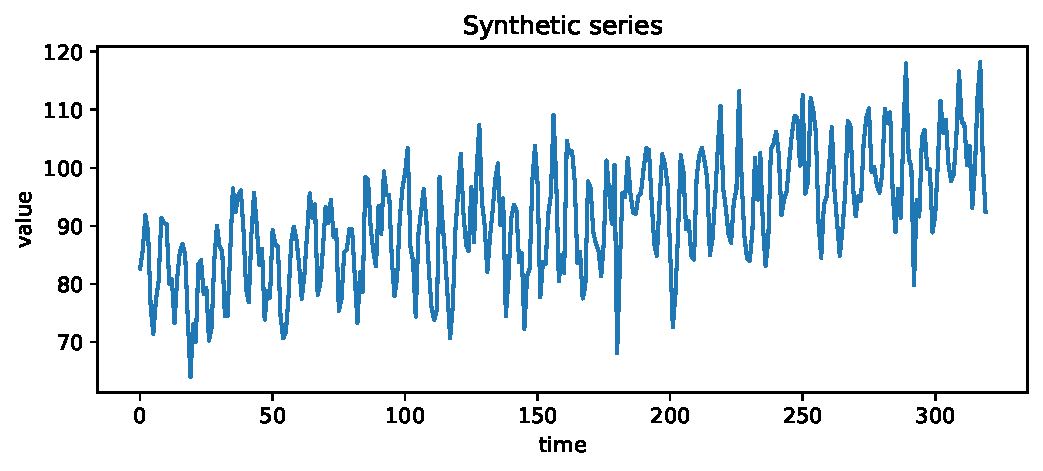
\includegraphics[keepaspectratio]{chapters/chapter-15-forecast-evaluation-backtesting_files/figure-pdf/ch15-simulate-series-output-1.pdf}}

}

\caption{Synthetic daily demand with trend, seasonality, noise, and
shocks.}

\end{figure}%

\protect\phantomsection\label{ch15-baseline-functions}
\begin{Shaded}
\begin{Highlighting}[]
\KeywordTok{def}\NormalTok{ forecast\_naive(train, horizon):}
    \ControlFlowTok{return}\NormalTok{ np.repeat(train[}\OperatorTok{{-}}\DecValTok{1}\NormalTok{], horizon)}


\KeywordTok{def}\NormalTok{ forecast\_seasonal\_naive(train, horizon, season):}
\NormalTok{    preds }\OperatorTok{=}\NormalTok{ []}
    \ControlFlowTok{for}\NormalTok{ h }\KeywordTok{in} \BuiltInTok{range}\NormalTok{(}\DecValTok{1}\NormalTok{, horizon }\OperatorTok{+} \DecValTok{1}\NormalTok{):}
\NormalTok{        idx }\OperatorTok{=} \BuiltInTok{len}\NormalTok{(train) }\OperatorTok{+}\NormalTok{ h }\OperatorTok{{-}}\NormalTok{ season }\OperatorTok{{-}} \DecValTok{1}
        \ControlFlowTok{while}\NormalTok{ idx }\OperatorTok{\textgreater{}=} \BuiltInTok{len}\NormalTok{(train):}
\NormalTok{            idx }\OperatorTok{{-}=}\NormalTok{ season}
\NormalTok{        preds.append(train[idx])}
    \ControlFlowTok{return}\NormalTok{ np.array(preds)}


\KeywordTok{def}\NormalTok{ forecast\_drift(train, horizon):}
    \ControlFlowTok{if} \BuiltInTok{len}\NormalTok{(train) }\OperatorTok{\textless{}} \DecValTok{2}\NormalTok{:}
        \ControlFlowTok{return}\NormalTok{ forecast\_naive(train, horizon)}
\NormalTok{    slope }\OperatorTok{=}\NormalTok{ (train[}\OperatorTok{{-}}\DecValTok{1}\NormalTok{] }\OperatorTok{{-}}\NormalTok{ train[}\DecValTok{0}\NormalTok{]) }\OperatorTok{/}\NormalTok{ (}\BuiltInTok{len}\NormalTok{(train) }\OperatorTok{{-}} \DecValTok{1}\NormalTok{)}
    \ControlFlowTok{return}\NormalTok{ np.array([train[}\OperatorTok{{-}}\DecValTok{1}\NormalTok{] }\OperatorTok{+}\NormalTok{ h }\OperatorTok{*}\NormalTok{ slope }\ControlFlowTok{for}\NormalTok{ h }\KeywordTok{in} \BuiltInTok{range}\NormalTok{(}\DecValTok{1}\NormalTok{, horizon }\OperatorTok{+} \DecValTok{1}\NormalTok{)])}


\KeywordTok{def}\NormalTok{ forecast\_moving\_average(train, horizon, window}\OperatorTok{=}\DecValTok{14}\NormalTok{):}
\NormalTok{    level }\OperatorTok{=}\NormalTok{ np.mean(train[}\OperatorTok{{-}}\NormalTok{window:])}
    \ControlFlowTok{return}\NormalTok{ np.repeat(level, horizon)}
\end{Highlighting}
\end{Shaded}

\begin{Shaded}
\begin{Highlighting}[]
\KeywordTok{def}\NormalTok{ rolling\_origin\_backtest(y, initial}\OperatorTok{=}\DecValTok{120}\NormalTok{, horizon}\OperatorTok{=}\DecValTok{14}\NormalTok{, step}\OperatorTok{=}\DecValTok{7}\NormalTok{, season}\OperatorTok{=}\DecValTok{7}\NormalTok{):}
\NormalTok{    y }\OperatorTok{=}\NormalTok{ np.asarray(y, dtype}\OperatorTok{=}\BuiltInTok{float}\NormalTok{)}
\NormalTok{    records }\OperatorTok{=}\NormalTok{ []}
    \ControlFlowTok{for}\NormalTok{ origin }\KeywordTok{in} \BuiltInTok{range}\NormalTok{(initial, }\BuiltInTok{len}\NormalTok{(y) }\OperatorTok{{-}}\NormalTok{ horizon, step):}
\NormalTok{        train }\OperatorTok{=}\NormalTok{ y[:origin]}
\NormalTok{        actual }\OperatorTok{=}\NormalTok{ y[origin:origin }\OperatorTok{+}\NormalTok{ horizon]}
\NormalTok{        forecasts }\OperatorTok{=}\NormalTok{ \{}
            \StringTok{"naive"}\NormalTok{: forecast\_naive(train, horizon),}
            \StringTok{"seasonal\_naive"}\NormalTok{: forecast\_seasonal\_naive(train, horizon, season),}
            \StringTok{"drift"}\NormalTok{: forecast\_drift(train, horizon),}
            \StringTok{"moving\_average"}\NormalTok{: forecast\_moving\_average(train, horizon, window}\OperatorTok{=}\DecValTok{14}\NormalTok{),}
\NormalTok{        \}}
        \ControlFlowTok{for}\NormalTok{ model, pred }\KeywordTok{in}\NormalTok{ forecasts.items():}
            \ControlFlowTok{for}\NormalTok{ h, (a, p) }\KeywordTok{in} \BuiltInTok{enumerate}\NormalTok{(}\BuiltInTok{zip}\NormalTok{(actual, pred), start}\OperatorTok{=}\DecValTok{1}\NormalTok{):}
\NormalTok{                records.append(\{}
                    \StringTok{"origin"}\NormalTok{: origin,}
                    \StringTok{"horizon"}\NormalTok{: h,}
                    \StringTok{"model"}\NormalTok{: model,}
                    \StringTok{"actual"}\NormalTok{: a,}
                    \StringTok{"forecast"}\NormalTok{: p,}
                    \StringTok{"error"}\NormalTok{: a }\OperatorTok{{-}}\NormalTok{ p,}
\NormalTok{                \})}
    \ControlFlowTok{return}\NormalTok{ pd.DataFrame(records)}


\NormalTok{bt }\OperatorTok{=}\NormalTok{ rolling\_origin\_backtest(y, initial}\OperatorTok{=}\DecValTok{120}\NormalTok{, horizon}\OperatorTok{=}\DecValTok{21}\NormalTok{, step}\OperatorTok{=}\DecValTok{7}\NormalTok{, season}\OperatorTok{=}\DecValTok{7}\NormalTok{)}
\NormalTok{bt.head()}
\end{Highlighting}
\end{Shaded}

\protect\phantomsection\label{ch15-backtest-function}
{\def\LTcaptype{none} % do not increment counter
\begin{longtable}[]{@{}lllllll@{}}
\toprule\noalign{}
& origin & horizon & model & actual & forecast & error \\
\midrule\noalign{}
\endhead
\bottomrule\noalign{}
\endlastfoot
0 & 120 & 1 & naive & 96.040937 & 89.494314 & 6.546623 \\
1 & 120 & 2 & naive & 102.440253 & 89.494314 & 12.945939 \\
2 & 120 & 3 & naive & 92.175057 & 89.494314 & 2.680744 \\
3 & 120 & 4 & naive & 86.711520 & 89.494314 & -2.782793 \\
4 & 120 & 5 & naive & 85.617345 & 89.494314 & -3.876968 \\
\end{longtable}
}

\begin{Shaded}
\begin{Highlighting}[]
\NormalTok{summary }\OperatorTok{=}\NormalTok{ (}
\NormalTok{    bt.groupby(}\StringTok{"model"}\NormalTok{)}
\NormalTok{    .}\BuiltInTok{apply}\NormalTok{(}\KeywordTok{lambda}\NormalTok{ g: pd.Series(\{}
        \StringTok{"ME"}\NormalTok{: g[}\StringTok{"error"}\NormalTok{].mean(),}
        \StringTok{"MAE"}\NormalTok{: mae(g[}\StringTok{"actual"}\NormalTok{], g[}\StringTok{"forecast"}\NormalTok{]),}
        \StringTok{"RMSE"}\NormalTok{: rmse(g[}\StringTok{"actual"}\NormalTok{], g[}\StringTok{"forecast"}\NormalTok{]),}
        \StringTok{"MAPE"}\NormalTok{: mape(g[}\StringTok{"actual"}\NormalTok{], g[}\StringTok{"forecast"}\NormalTok{]),}
        \StringTok{"sMAPE"}\NormalTok{: smape(g[}\StringTok{"actual"}\NormalTok{], g[}\StringTok{"forecast"}\NormalTok{]),}
        \StringTok{"MASE"}\NormalTok{: mase(y[:}\DecValTok{120}\NormalTok{], g[}\StringTok{"actual"}\NormalTok{], g[}\StringTok{"forecast"}\NormalTok{], season}\OperatorTok{=}\DecValTok{7}\NormalTok{),}
        \StringTok{"RMSSE"}\NormalTok{: rmsse(y[:}\DecValTok{120}\NormalTok{], g[}\StringTok{"actual"}\NormalTok{], g[}\StringTok{"forecast"}\NormalTok{], season}\OperatorTok{=}\DecValTok{7}\NormalTok{),}
\NormalTok{    \}))}
\NormalTok{    .sort\_values(}\StringTok{"MAE"}\NormalTok{)}
\NormalTok{)}

\NormalTok{summary.}\BuiltInTok{round}\NormalTok{(}\DecValTok{3}\NormalTok{)}
\end{Highlighting}
\end{Shaded}

\protect\phantomsection\label{ch15-backtest-summary}
{\def\LTcaptype{none} % do not increment counter
\begin{longtable}[]{@{}llllllll@{}}
\toprule\noalign{}
& ME & MAE & RMSE & MAPE & sMAPE & MASE & RMSSE \\
model & & & & & & & \\
\midrule\noalign{}
\endhead
\bottomrule\noalign{}
\endlastfoot
seasonal\_naive & 1.004 & 6.367 & 8.217 & 6.800 & 6.839 & 1.081 &
1.176 \\
moving\_average & 1.291 & 7.347 & 8.916 & 7.805 & 7.806 & 1.247 &
1.276 \\
naive & 1.478 & 8.381 & 10.225 & 8.904 & 8.915 & 1.423 & 1.463 \\
drift & 0.889 & 8.489 & 10.397 & 9.064 & 9.016 & 1.441 & 1.488 \\
\end{longtable}
}

\section{15.15 Python example: horizon-wise error
curves}\label{python-example-horizon-wise-error-curves}

A single score can hide important structure. Horizon-wise curves show
how accuracy changes as the forecast looks farther ahead.

\begin{Shaded}
\begin{Highlighting}[]
\NormalTok{horizon\_summary }\OperatorTok{=}\NormalTok{ (}
\NormalTok{    bt.groupby([}\StringTok{"model"}\NormalTok{, }\StringTok{"horizon"}\NormalTok{])}
\NormalTok{    .}\BuiltInTok{apply}\NormalTok{(}\KeywordTok{lambda}\NormalTok{ g: pd.Series(\{}\StringTok{"MAE"}\NormalTok{: mae(g[}\StringTok{"actual"}\NormalTok{], g[}\StringTok{"forecast"}\NormalTok{])\}))}
\NormalTok{    .reset\_index()}
\NormalTok{)}

\NormalTok{fig, ax }\OperatorTok{=}\NormalTok{ plt.subplots(figsize}\OperatorTok{=}\NormalTok{(}\DecValTok{8}\NormalTok{, }\DecValTok{4}\NormalTok{))}
\ControlFlowTok{for}\NormalTok{ model, g }\KeywordTok{in}\NormalTok{ horizon\_summary.groupby(}\StringTok{"model"}\NormalTok{):}
\NormalTok{    ax.plot(g[}\StringTok{"horizon"}\NormalTok{], g[}\StringTok{"MAE"}\NormalTok{], marker}\OperatorTok{=}\StringTok{"o"}\NormalTok{, label}\OperatorTok{=}\NormalTok{model)}
\NormalTok{ax.set\_xlabel(}\StringTok{"forecast horizon"}\NormalTok{)}
\NormalTok{ax.set\_ylabel(}\StringTok{"MAE"}\NormalTok{)}
\NormalTok{ax.set\_title(}\StringTok{"Forecast accuracy by horizon"}\NormalTok{)}
\NormalTok{ax.legend()}
\NormalTok{plt.show()}
\end{Highlighting}
\end{Shaded}

\begin{figure}[H]

{\centering \pandocbounded{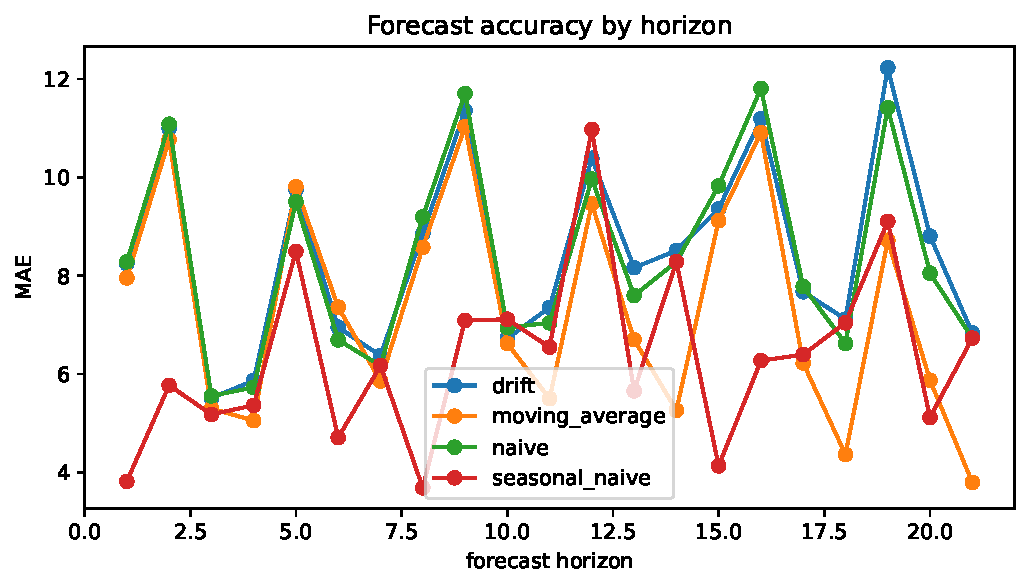
\includegraphics[keepaspectratio]{chapters/chapter-15-forecast-evaluation-backtesting_files/figure-pdf/ch15-horizon-curves-output-1.pdf}}

}

\caption{Horizon-wise MAE curves for simple baseline forecasts.}

\end{figure}%

\section{15.16 Python example: interval coverage from residual
backtesting}\label{python-example-interval-coverage-from-residual-backtesting}

A simple residual-based interval can be constructed by estimating the
distribution of past forecast errors. This is not always valid, but it
is a useful starting point.

\begin{Shaded}
\begin{Highlighting}[]
\NormalTok{model\_name }\OperatorTok{=} \StringTok{"seasonal\_naive"}
\NormalTok{errors }\OperatorTok{=}\NormalTok{ bt.loc[bt[}\StringTok{"model"}\NormalTok{] }\OperatorTok{==}\NormalTok{ model\_name, }\StringTok{"error"}\NormalTok{].to\_numpy()}
\NormalTok{lo\_q, hi\_q }\OperatorTok{=}\NormalTok{ np.quantile(errors, [}\FloatTok{0.05}\NormalTok{, }\FloatTok{0.95}\NormalTok{])}

\NormalTok{origin }\OperatorTok{=} \DecValTok{280}
\NormalTok{train }\OperatorTok{=}\NormalTok{ y[:origin]}
\NormalTok{horizon }\OperatorTok{=} \DecValTok{28}
\NormalTok{point }\OperatorTok{=}\NormalTok{ forecast\_seasonal\_naive(train, horizon, season}\OperatorTok{=}\DecValTok{7}\NormalTok{)}
\NormalTok{future\_t }\OperatorTok{=}\NormalTok{ np.arange(origin, origin }\OperatorTok{+}\NormalTok{ horizon)}
\NormalTok{actual }\OperatorTok{=}\NormalTok{ y[origin:origin }\OperatorTok{+}\NormalTok{ horizon]}
\NormalTok{lo }\OperatorTok{=}\NormalTok{ point }\OperatorTok{+}\NormalTok{ lo\_q}
\NormalTok{hi }\OperatorTok{=}\NormalTok{ point }\OperatorTok{+}\NormalTok{ hi\_q}

\NormalTok{coverage }\OperatorTok{=}\NormalTok{ np.mean((actual }\OperatorTok{\textgreater{}=}\NormalTok{ lo) }\OperatorTok{\&}\NormalTok{ (actual }\OperatorTok{\textless{}=}\NormalTok{ hi))}
\NormalTok{avg\_width }\OperatorTok{=}\NormalTok{ np.mean(hi }\OperatorTok{{-}}\NormalTok{ lo)}
\BuiltInTok{print}\NormalTok{(}\SpecialStringTok{f"Empirical coverage on this final path: }\SpecialCharTok{\{}\NormalTok{coverage}\SpecialCharTok{:.3f\}}\SpecialStringTok{"}\NormalTok{)}
\BuiltInTok{print}\NormalTok{(}\SpecialStringTok{f"Average interval width: }\SpecialCharTok{\{}\NormalTok{avg\_width}\SpecialCharTok{:.2f\}}\SpecialStringTok{"}\NormalTok{)}

\NormalTok{plt.figure(figsize}\OperatorTok{=}\NormalTok{(}\DecValTok{8}\NormalTok{, }\DecValTok{4}\NormalTok{))}
\NormalTok{plt.plot(t[:origin], y[:origin], label}\OperatorTok{=}\StringTok{"training history"}\NormalTok{)}
\NormalTok{plt.plot(future\_t, actual, marker}\OperatorTok{=}\StringTok{"o"}\NormalTok{, label}\OperatorTok{=}\StringTok{"actual future"}\NormalTok{)}
\NormalTok{plt.plot(future\_t, point, marker}\OperatorTok{=}\StringTok{"o"}\NormalTok{, label}\OperatorTok{=}\StringTok{"point forecast"}\NormalTok{)}
\NormalTok{plt.fill\_between(future\_t, lo, hi, alpha}\OperatorTok{=}\FloatTok{0.25}\NormalTok{, label}\OperatorTok{=}\StringTok{"90}\SpecialCharTok{\% r}\StringTok{esidual interval"}\NormalTok{)}
\NormalTok{plt.axvline(origin }\OperatorTok{{-}} \DecValTok{1}\NormalTok{, linestyle}\OperatorTok{=}\StringTok{"{-}{-}"}\NormalTok{)}
\NormalTok{plt.xlabel(}\StringTok{"time"}\NormalTok{)}
\NormalTok{plt.ylabel(}\StringTok{"value"}\NormalTok{)}
\NormalTok{plt.title(}\StringTok{"Residual{-}based forecast interval"}\NormalTok{)}
\NormalTok{plt.legend()}
\NormalTok{plt.show()}
\end{Highlighting}
\end{Shaded}

\begin{verbatim}
Empirical coverage on this final path: 0.893
Average interval width: 26.27
\end{verbatim}

\begin{figure}[H]

{\centering \pandocbounded{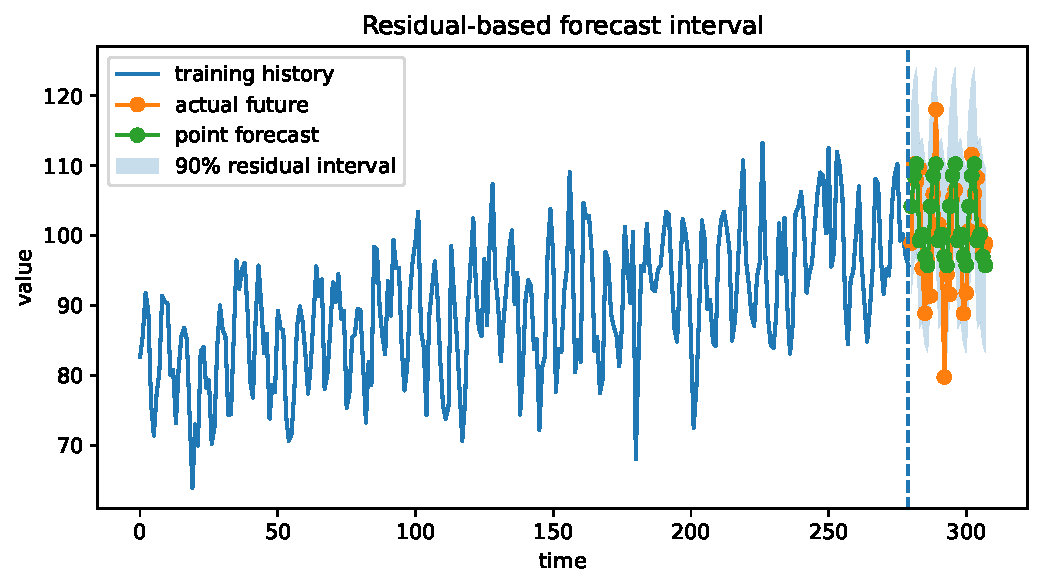
\includegraphics[keepaspectratio]{chapters/chapter-15-forecast-evaluation-backtesting_files/figure-pdf/ch15-interval-coverage-output-2.pdf}}

}

\caption{A simple residual-based prediction interval for the final
forecast path.}

\end{figure}%

\begin{tcolorbox}[enhanced jigsaw, arc=.35mm, bottomrule=.15mm, bottomtitle=1mm, breakable, colback=white, colbacktitle=quarto-callout-warning-color!10!white, colframe=quarto-callout-warning-color-frame, coltitle=black, left=2mm, leftrule=.75mm, opacityback=0, opacitybacktitle=0.6, rightrule=.15mm, title=\textcolor{quarto-callout-warning-color}{\faExclamationTriangle}\hspace{0.5em}{Residual intervals are only a starting point}, titlerule=0mm, toprule=.15mm, toptitle=1mm]

Residual-based intervals assume the future error distribution resembles
the historical backtest error distribution. Regime changes,
heteroskedasticity, changing seasonality, and model updates can break
this assumption.

\end{tcolorbox}

\section{15.17 AI-assisted modeling
activity}\label{ai-assisted-modeling-activity}

\section{AI-assisted evaluation
critic}\label{ai-assisted-evaluation-critic}

Give an AI assistant your evaluation design and ask it to answer the
following questions:

\begin{enumerate}
\def\labelenumi{\arabic{enumi}.}
\tightlist
\item
  What is the forecast origin?
\item
  What is the forecast horizon?
\item
  Which variables are available at the forecast origin?
\item
  Is the preprocessing fitted only on the training portion?
\item
  Are any centered smoothers or future-looking rolling statistics used?
\item
  What baseline must the model beat?
\item
  Which metric matches the decision problem?
\item
  Should the metric be reported horizon by horizon?
\item
  Is the final test set used only once?
\item
  What failure mode would make the evaluation too optimistic?
\end{enumerate}

Then verify each answer in code. AI can help audit a workflow, but it
cannot certify that the data were truly available at the forecast
origin.

\subsection{Prompt template}\label{prompt-template}

Use a prompt like this:

\begin{quote}
I am forecasting \(Y_{t+h}\) using data available at time \(t\). My
features are {[}list features{]}, my split is {[}describe split{]}, and
my metric is {[}metric{]}. Audit this evaluation for time-series
leakage. For every possible leakage source, explain the mathematical
reason it is or is not leakage.
\end{quote}

\subsection{Verification checklist}\label{verification-checklist}

After using AI, manually check:

\begin{itemize}
\tightlist
\item
  the index ranges used to compute every lag and rolling feature;
\item
  whether scalers, imputers, encoders, and transformations are fitted
  only on training data;
\item
  whether hyperparameters were selected using validation data rather
  than the final test set;
\item
  whether each baseline is implemented using only past data;
\item
  whether forecast errors are grouped by horizon correctly.
\end{itemize}

\section{15.18 Common mistakes}\label{common-mistakes-14}

\begin{enumerate}
\def\labelenumi{\arabic{enumi}.}
\tightlist
\item
  \textbf{Using random train-test splits.} This usually leaks future
  information.
\item
  \textbf{Reporting only one metric.} A single number may hide
  horizon-specific failures.
\item
  \textbf{Ignoring baselines.} A deep model that does not beat seasonal
  naive is not useful.
\item
  \textbf{Using MAPE blindly.} MAPE can explode when actual values are
  near zero.
\item
  \textbf{Confusing residuals with backtest errors.} Residual
  diagnostics are not enough.
\item
  \textbf{Tuning on the test set.} The test set becomes part of model
  selection.
\item
  \textbf{Using non-causal smoothing.} Centered smoothing uses future
  observations.
\item
  \textbf{Comparing models under different backtests.} Every model
  should be evaluated on the same forecast origins and horizons.
\item
  \textbf{Ignoring uncertainty.} A point forecast without interval
  quality may be insufficient for decisions.
\item
  \textbf{Evaluating the wrong horizon.} A one-step score may not
  reflect operational multi-step forecasting.
\end{enumerate}

\section{15.19 Mini project: model comparison
report}\label{mini-project-model-comparison-report}

Choose one real time series with at least one seasonal pattern. Examples
include electricity demand, public transit ridership, retail sales, air
passengers, web traffic, or weather measurements.

Your report should include:

\begin{enumerate}
\def\labelenumi{\arabic{enumi}.}
\tightlist
\item
  a short description of the forecasting task;
\item
  forecast horizon and forecast origin definition;
\item
  a time-aware train/validation/test design;
\item
  at least three baselines: naive, seasonal naive, and drift;
\item
  one statistical model or one machine-learning model;
\item
  horizon-wise MAE and RMSE;
\item
  MASE or RMSSE using a training-only scale;
\item
  a leakage audit;
\item
  one prediction interval or quantile forecast evaluation;
\item
  a final recommendation.
\end{enumerate}

\section{15.20 Exercises}\label{exercises-14}

\begin{enumerate}
\def\labelenumi{\arabic{enumi}.}
\item
  Let \(e_{t,h}=Y_{t+h}-\widehat Y_{t+h\mid t}\). Prove that RMSE is
  always at least MAE when both are computed over the same errors.
\item
  Give an example where MAPE is undefined. Give another example where
  MAPE is finite but misleadingly large.
\item
  Suppose \(Y_t=Y_{t-1}+W_t\) is a random walk. Which baseline should be
  strong for one-step forecasting? Explain mathematically.
\item
  For seasonal monthly data, define the seasonal naive forecast for
  horizons \(h=1,\ldots,12\) at forecast origin \(t\).
\item
  Suppose a feature is a seven-day centered moving average of \(Y_t\).
  Explain why it is invalid for forecasting \(Y_{t+1}\) at time \(t\).
\item
  Implement expanding-window and sliding-window backtests for the same
  data. When might the sliding-window version perform better?
\item
  Construct a synthetic time series with a structural break. Compare
  expanding-window and sliding-window evaluation.
\item
  Show that the median forecast minimizes expected absolute loss.
\item
  Show that the mean forecast minimizes expected squared loss.
\item
  Design a backtest for forecasting weekly demand four weeks ahead.
  Specify forecast origins, horizon, training window, validation period,
  final test period, and metric.
\end{enumerate}

\section{15.21 Chapter checklist}\label{chapter-checklist-12}

You should now be able to:

\begin{itemize}
\tightlist
\item
  write forecast errors with correct origin and horizon notation;
\item
  explain why time-aware evaluation is essential;
\item
  implement naive, seasonal naive, drift, and moving-average baselines;
\item
  compute MAE, RMSE, MAPE, sMAPE, MASE, and RMSSE;
\item
  perform rolling-origin backtesting;
\item
  report horizon-wise error curves;
\item
  distinguish fitted residuals from true out-of-sample errors;
\item
  identify common leakage sources;
\item
  evaluate interval coverage and width;
\item
  use AI as an evaluation auditor while verifying every claim yourself.
\end{itemize}

\chapter{Automated Forecasting and Prophet-Type Additive
Models}\label{automated-forecasting-and-prophet-type-additive-models}

\textbf{Part V. Forecasting at Scale and Machine Learning Methods}\\
\textbf{Chapter goal:} understand automated forecasting as a modeling
pipeline, not as a black box. We study Prophet-type additive models,
changepoints, Fourier seasonality, holiday effects, cross-validation,
hyperparameter tuning, and the analyst-in-the-loop workflow used when
many time series must be forecast repeatedly.

\section{Learning objectives}\label{learning-objectives-15}

After studying this chapter, you should be able to:

\begin{enumerate}
\def\labelenumi{\arabic{enumi}.}
\tightlist
\item
  explain why manual ARIMA/SARIMA modeling becomes difficult at scale;
\item
  distinguish time-domain models, frequency-domain methods, additive
  forecasting models, and deep-learning sequence models;
\item
  write the Prophet-style additive model \[
  y(t)=g(t)+s(t)+h(t)+\varepsilon_t;
  \]
\item
  derive the main ingredients of piecewise linear trend, saturating
  logistic trend, Fourier seasonality, and holiday indicators;
\item
  explain why changepoint priors and seasonality priors act as
  regularization parameters;
\item
  construct a simplified Prophet-like model using linear regression,
  Fourier features, changepoint basis functions, and holiday indicators;
\item
  design rolling-origin cross-validation for automated forecasting;
\item
  tune changepoint, seasonality, holiday, and seasonality-mode
  parameters without leaking future information;
\item
  compare Prophet-type models with SARIMA and machine-learning feature
  models;
\item
  use AI assistants to generate candidate forecasting pipelines while
  independently checking assumptions, leakage, and diagnostics.
\end{enumerate}

\section{16.1 Why automated
forecasting?}\label{why-automated-forecasting}

Classical chapters built models by hand. For a single important series,
hand modeling is valuable: plot the data, transform it, inspect the
ACF/PACF, choose ARIMA or SARIMA orders, estimate parameters, diagnose
residuals, and backtest forecasts. This workflow gives mathematical
control.

At scale, however, an organization may need forecasts for hundreds,
thousands, or millions of related time series:

\begin{itemize}
\tightlist
\item
  daily demand for many products;
\item
  hourly load for many regions;
\item
  weekly admissions for many programs;
\item
  traffic, rideshare, health, finance, climate, or website metrics;
\item
  multiple horizons and repeated updates.
\end{itemize}

Manual modeling becomes slow and inconsistent. Automated forecasting
asks for a procedure that can:

\begin{enumerate}
\def\labelenumi{\arabic{enumi}.}
\tightlist
\item
  fit reasonable models with minimal manual intervention;
\item
  incorporate common forecasting structure such as trend, seasonality,
  holidays, and outliers;
\item
  support analyst knowledge through interpretable parameters;
\item
  evaluate forecasts with rolling-origin backtests;
\item
  scale across many time series.
\end{enumerate}

The lecture notes place Prophet after ARIMA/SARIMA, spectral analysis,
and deep-learning approaches. That is the right position pedagogically:
Prophet is not a replacement for time-series theory; it is a practical
additive modeling strategy that borrows ideas from regression, splines,
Fourier analysis, Bayesian regularization, and forecasting evaluation.

\begin{tcolorbox}[enhanced jigsaw, arc=.35mm, bottomrule=.15mm, bottomtitle=1mm, breakable, colback=white, colbacktitle=quarto-callout-note-color!10!white, colframe=quarto-callout-note-color-frame, coltitle=black, left=2mm, leftrule=.75mm, opacityback=0, opacitybacktitle=0.6, rightrule=.15mm, title=\textcolor{quarto-callout-note-color}{\faInfo}\hspace{0.5em}{Automated does not mean assumption-free}, titlerule=0mm, toprule=.15mm, toptitle=1mm]

An automated model still makes assumptions. Prophet-type models assume
that trend, seasonality, holiday effects, and noise give a useful
decomposition. A good analyst checks whether this decomposition matches
the forecasting problem.

\end{tcolorbox}

\section{16.2 A taxonomy of forecasting
models}\label{a-taxonomy-of-forecasting-models}

A useful high-level taxonomy is:

\begin{enumerate}
\def\labelenumi{\arabic{enumi}.}
\tightlist
\item
  \textbf{Time-domain statistical models}: AR, MA, ARMA, ARIMA, SARIMA,
  state-space models. These model dependence through lagged values and
  lagged shocks.
\item
  \textbf{Frequency-domain methods}: Fourier analysis, spectral density,
  periodograms, wavelets, filtering. These model oscillatory structure.
\item
  \textbf{Additive automated models}: Prophet-type models, generalized
  additive models, spline trend plus seasonality and holiday effects.
\item
  \textbf{Machine-learning feature models}: lag features, rolling
  statistics, calendar features, gradient boosting, random forests.
\item
  \textbf{Deep sequence models}: RNN, LSTM, GRU, temporal CNN, TCN,
  attention, and transformers.
\end{enumerate}

The categories overlap. Prophet uses Fourier features for seasonality,
regression-like additive components, changepoint regularization, and
rolling-origin cross-validation. NeuralProphet and related models add
autoregression or neural-network components.

A practical forecaster compares at least:

\[
\text{naive},\quad
\text{seasonal naive},\quad
\text{SARIMA},\quad
\text{Prophet-type additive model},\quad
\text{ML feature model}.
\]

The winning model depends on the data-generating mechanism, forecast
horizon, cost function, and operational constraints.

\section{16.3 The Prophet-style additive
model}\label{the-prophet-style-additive-model}

A Prophet-type model represents the observed series as

\[
y(t)=g(t)+s(t)+h(t)+\varepsilon_t.
\]

The components are:

\begin{itemize}
\tightlist
\item
  \(g(t)\): trend, modeling nonperiodic long-term change;
\item
  \(s(t)\): seasonal component, modeling periodic behavior;
\item
  \(h(t)\): holiday or event component, modeling irregular known events;
\item
  \(\varepsilon_t\): residual error.
\end{itemize}

This is a \textbf{generalized additive forecasting model}. The model is
interpretable because each term has a separate role.

For a fixed set of basis functions, the additive model can be written as
a regression:

\[
y_t
=\beta_0
+\sum_{j=1}^{p_g}\beta^{(g)}_j G_j(t)
+\sum_{j=1}^{p_s}\beta^{(s)}_j S_j(t)
+\sum_{j=1}^{p_h}\beta^{(h)}_j H_j(t)
+\varepsilon_t.
\]

Here:

\begin{itemize}
\tightlist
\item
  \(G_j(t)\) are trend/changepoint features;
\item
  \(S_j(t)\) are seasonal Fourier features;
\item
  \(H_j(t)\) are holiday/event indicators.
\end{itemize}

The model is simple in form, but the feature design and regularization
are important.

\section{Additive model as
projection}\label{additive-model-as-projection}

If the noise has mean zero and the features are fixed, the least-squares
fit is the orthogonal projection of the data vector \(y\) onto the span
of the trend, seasonal, and holiday feature vectors. Regularization
shrinks this projection toward simpler trend and seasonal components.

\section{16.4 Trend component I: piecewise linear
trend}\label{trend-component-i-piecewise-linear-trend}

A common trend model is piecewise linear. Suppose changepoints occur at

\[
s_1<s_2<\cdots<s_J.
\]

Define the hinge basis function

\[
(t-s_j)_+=\max(t-s_j,0).
\]

A continuous piecewise linear trend can be written as

\[
g(t)=m+kt+\sum_{j=1}^J\delta_j(t-s_j)_+.
\]

Before the first changepoint, the slope is \(k\). After changepoint
\(s_j\), the slope changes by \(\delta_j\). Therefore, after all
changepoints up to time \(t\), the local slope is

\[
k+\sum_{j:s_j<t}\delta_j.
\]

This form is closely related to linear splines. It is useful because:

\begin{enumerate}
\def\labelenumi{\arabic{enumi}.}
\tightlist
\item
  the trend remains continuous;
\item
  changes in growth rate are explicit;
\item
  changepoints can be chosen automatically or specified by the analyst;
\item
  regularizing the coefficients \(\delta_j\) controls flexibility.
\end{enumerate}

\subsection{Changepoint
regularization}\label{changepoint-regularization}

If too many changepoints are allowed without regularization, the trend
can overfit noise. A Laplace prior

\[
\delta_j\sim \operatorname{Laplace}(0,\tau)
\]

encourages many \(\delta_j\) to be close to zero. In optimization terms,
this behaves like an \(\ell^1\) penalty:

\[
\min_\beta
\sum_{t=1}^T
\left(y_t-\widehat y_t\right)^2
+\lambda\sum_{j=1}^J|\delta_j|.
\]

Small \(\tau\) or large \(\lambda\) gives a smoother trend. Large
\(\tau\) or small \(\lambda\) allows more changepoint flexibility.

\begin{tcolorbox}[enhanced jigsaw, arc=.35mm, bottomrule=.15mm, bottomtitle=1mm, breakable, colback=white, colbacktitle=quarto-callout-warning-color!10!white, colframe=quarto-callout-warning-color-frame, coltitle=black, left=2mm, leftrule=.75mm, opacityback=0, opacitybacktitle=0.6, rightrule=.15mm, title=\textcolor{quarto-callout-warning-color}{\faExclamationTriangle}\hspace{0.5em}{Changepoints are not magic}, titlerule=0mm, toprule=.15mm, toptitle=1mm]

A changepoint basis can explain historical bends in the curve, but it
does not know whether those bends will continue. Long-horizon forecasts
can be very sensitive to trend assumptions.

\end{tcolorbox}

\section{16.5 Trend component II: saturating logistic
growth}\label{trend-component-ii-saturating-logistic-growth}

For growth that cannot increase forever, Prophet-type models may use a
saturating logistic trend. The basic logistic curve is

\[
g(t)=\frac{C}{1+\exp(-k(t-m))},
\]

where:

\begin{itemize}
\tightlist
\item
  \(C\) is the carrying capacity;
\item
  \(k\) is the growth rate;
\item
  \(m\) is an offset parameter controlling the midpoint.
\end{itemize}

This model is appropriate when there is a natural ceiling: population
growth in an ecosystem, market adoption, number of users in a bounded
region, or capacity-limited demand.

A time-varying capacity version replaces \(C\) by \(C(t)\):

\[
g(t)=\frac{C(t)}{1+\exp(-k(t-m))}.
\]

Changepoints can also modify the growth rate. Conceptually,

\[
k(t)=k+\sum_{j:s_j<t}\delta_j.
\]

The technical implementation adjusts the offset terms so that the curve
remains continuous at changepoints.

\begin{tcolorbox}[enhanced jigsaw, arc=.35mm, bottomrule=.15mm, bottomtitle=1mm, breakable, colback=white, colbacktitle=quarto-callout-tip-color!10!white, colframe=quarto-callout-tip-color-frame, coltitle=black, left=2mm, leftrule=.75mm, opacityback=0, opacitybacktitle=0.6, rightrule=.15mm, title=\textcolor{quarto-callout-tip-color}{\faLightbulb}\hspace{0.5em}{Linear or logistic trend?}, titlerule=0mm, toprule=.15mm, toptitle=1mm]

Use a logistic trend only when a meaningful capacity is available.
Without a meaningful carrying capacity, a piecewise linear trend is
usually easier to explain and diagnose.

\end{tcolorbox}

\section{16.6 Seasonality through Fourier
features}\label{seasonality-through-fourier-features}

A periodic function with period \(P\) satisfies

\[
s(t+P)=s(t).
\]

Prophet models seasonality using a truncated Fourier series:

\[
s(t)=
\sum_{n=1}^N
\left[
 a_n\cos\left(\frac{2\pi nt}{P}\right)
+b_n\sin\left(\frac{2\pi nt}{P}\right)
\right].
\]

For weekly seasonality in daily data, \(P=7\). For yearly seasonality in
daily data, \(P\approx365.25\). For hourly data with daily seasonality,
\(P=24\) if time is measured in hours.

The Fourier order \(N\) controls flexibility:

\begin{itemize}
\tightlist
\item
  small \(N\): smooth seasonal curve;
\item
  large \(N\): more wiggly seasonal curve;
\item
  too large \(N\): overfitting.
\end{itemize}

The number of seasonal coefficients for one seasonal period is \(2N\).

Fourier seasonality connects this chapter directly to spectral analysis.
The difference is that here the Fourier basis is used as a deterministic
regression basis, not as a full stochastic spectral model.

\section{16.7 Holiday and event
effects}\label{holiday-and-event-effects}

Some effects are neither smooth trends nor regular seasonality. Examples
include:

\begin{itemize}
\tightlist
\item
  Thanksgiving, Black Friday, Christmas, Lunar New Year;
\item
  semester start, graduation, application deadlines;
\item
  product launches;
\item
  policy changes;
\item
  weather events;
\item
  one-time disruptions.
\end{itemize}

For holiday \(i\), let \(D_i\) be the set of dates associated with that
holiday. Define

\[
H_i(t)=\mathbf 1_{\{t\in D_i\}}.
\]

A holiday component is

\[
h(t)=\sum_{i=1}^K\kappa_i H_i(t).
\]

In matrix form,

\[
h(t)=Z(t)^T\kappa.
\]

A Gaussian prior

\[
\kappa_i\sim N(0,\nu^2)
\]

shrinks holiday effects toward zero unless the data support them. This
is important when many holidays or event windows are included.

Holiday effects can also include windows. For example, a Black Friday
effect may include Thanksgiving Day, Black Friday, and Cyber Monday:

\[
H_{\text{BlackFriday}}(t)=1
\quad\text{if }t\in\{\text{Thu},\text{Fri},\text{Mon}\}
\]

for the relevant calendar year.

\section{16.8 Additive versus multiplicative
seasonality}\label{additive-versus-multiplicative-seasonality}

The default additive model is

\[
y(t)=g(t)+s(t)+h(t)+\varepsilon_t.
\]

This assumes that seasonal fluctuations have roughly constant absolute
size. For example, the seasonal amplitude is about \(10\) units whether
the trend is \(100\) or \(1000\).

A multiplicative seasonal model has the form

\[
y(t)=g(t)\{1+s(t)+h(t)\}+\varepsilon_t.
\]

This assumes that seasonal fluctuations scale with the level. For
example, the seasonal effect might be about \(10\%\) of the trend.

A common alternative is to log-transform the response:

\[
z(t)=\log y(t),
\]

then fit an additive model to \(z(t)\). On the original scale, additive
structure in logs becomes multiplicative structure.

\begin{tcolorbox}[enhanced jigsaw, arc=.35mm, bottomrule=.15mm, bottomtitle=1mm, breakable, colback=white, colbacktitle=quarto-callout-note-color!10!white, colframe=quarto-callout-note-color-frame, coltitle=black, left=2mm, leftrule=.75mm, opacityback=0, opacitybacktitle=0.6, rightrule=.15mm, title=\textcolor{quarto-callout-note-color}{\faInfo}\hspace{0.5em}{Rule of thumb}, titlerule=0mm, toprule=.15mm, toptitle=1mm]

If seasonal swings get larger as the series level increases, consider
multiplicative seasonality or a log transformation.

\end{tcolorbox}

\section{16.9 Interactive module: build a Prophet-type additive
model}\label{interactive-module-build-a-prophet-type-additive-model}

The interactive below simulates a Prophet-type model. The graph uses the
global Plotly toolbar from \texttt{assets/header.html}, so students can
zoom, pan, reset axes, and download the plot.

Interactive Module: Additive Forecasting Components

Adjust trend, changepoint flexibility, seasonality, holiday pulse, and
noise. The plot shows the observed series and its underlying additive
components.

\begin{verbatim}
<label>Base slope
  <input id="ch16-slope" type="range" min="-0.05" max="0.10" step="0.005" value="0.035">
</label>
<label>Changepoint effect
  <input id="ch16-change" type="range" min="-0.12" max="0.12" step="0.01" value="-0.04">
</label>
<label>Seasonal amplitude
  <input id="ch16-season" type="range" min="0" max="8" step="0.5" value="4">
</label>
<label>Fourier order
  <input id="ch16-fourier" type="range" min="1" max="5" step="1" value="2">
</label>
<label>Holiday effect
  <input id="ch16-holiday" type="range" min="-15" max="20" step="1" value="10">
</label>
<label>Noise scale
  <input id="ch16-noise" type="range" min="0" max="6" step="0.5" value="2">
</label>
\end{verbatim}

\protect\phantomsection\label{ch16-prophet-additive-plot}

\section{16.10 Python example: simulate additive forecasting
data}\label{python-example-simulate-additive-forecasting-data}

We now build a synthetic data set with trend, changepoints, weekly
seasonality, yearly seasonality, holiday effects, and noise.

\begin{Shaded}
\begin{Highlighting}[]
\ImportTok{import}\NormalTok{ numpy }\ImportTok{as}\NormalTok{ np}
\ImportTok{import}\NormalTok{ pandas }\ImportTok{as}\NormalTok{ pd}
\ImportTok{import}\NormalTok{ matplotlib.pyplot }\ImportTok{as}\NormalTok{ plt}

\NormalTok{rng }\OperatorTok{=}\NormalTok{ np.random.default\_rng(}\DecValTok{7339}\NormalTok{)}

\NormalTok{n }\OperatorTok{=} \DecValTok{3} \OperatorTok{*} \DecValTok{365}
\NormalTok{dates }\OperatorTok{=}\NormalTok{ pd.date\_range(}\StringTok{"2020{-}01{-}01"}\NormalTok{, periods}\OperatorTok{=}\NormalTok{n, freq}\OperatorTok{=}\StringTok{"D"}\NormalTok{)}
\NormalTok{t }\OperatorTok{=}\NormalTok{ np.arange(n)}

\CommentTok{\# Piecewise linear trend with two changepoints}
\NormalTok{cp1, cp2 }\OperatorTok{=} \DecValTok{320}\NormalTok{, }\DecValTok{760}
\NormalTok{trend }\OperatorTok{=} \DecValTok{40} \OperatorTok{+} \FloatTok{0.025} \OperatorTok{*}\NormalTok{ t }\OperatorTok{+} \FloatTok{0.060} \OperatorTok{*}\NormalTok{ np.maximum(t }\OperatorTok{{-}}\NormalTok{ cp1, }\DecValTok{0}\NormalTok{) }\OperatorTok{{-}} \FloatTok{0.080} \OperatorTok{*}\NormalTok{ np.maximum(t }\OperatorTok{{-}}\NormalTok{ cp2, }\DecValTok{0}\NormalTok{)}

\CommentTok{\# Weekly and yearly seasonal components}
\NormalTok{weekly }\OperatorTok{=} \FloatTok{3.0} \OperatorTok{*}\NormalTok{ np.sin(}\DecValTok{2} \OperatorTok{*}\NormalTok{ np.pi }\OperatorTok{*}\NormalTok{ t }\OperatorTok{/} \DecValTok{7}\NormalTok{) }\OperatorTok{+} \FloatTok{1.2} \OperatorTok{*}\NormalTok{ np.cos(}\DecValTok{2} \OperatorTok{*}\NormalTok{ np.pi }\OperatorTok{*}\NormalTok{ t }\OperatorTok{/} \DecValTok{7}\NormalTok{)}
\NormalTok{yearly }\OperatorTok{=} \FloatTok{6.0} \OperatorTok{*}\NormalTok{ np.sin(}\DecValTok{2} \OperatorTok{*}\NormalTok{ np.pi }\OperatorTok{*}\NormalTok{ t }\OperatorTok{/} \FloatTok{365.25}\NormalTok{) }\OperatorTok{+} \FloatTok{2.5} \OperatorTok{*}\NormalTok{ np.cos(}\DecValTok{4} \OperatorTok{*}\NormalTok{ np.pi }\OperatorTok{*}\NormalTok{ t }\OperatorTok{/} \FloatTok{365.25}\NormalTok{)}

\CommentTok{\# Holiday pulses: one event per year}
\NormalTok{holiday }\OperatorTok{=}\NormalTok{ np.zeros(n)}
\ControlFlowTok{for}\NormalTok{ day }\KeywordTok{in}\NormalTok{ [}\DecValTok{80}\NormalTok{, }\DecValTok{445}\NormalTok{, }\DecValTok{810}\NormalTok{]:}
\NormalTok{    holiday[np.}\BuiltInTok{abs}\NormalTok{(t }\OperatorTok{{-}}\NormalTok{ day) }\OperatorTok{\textless{}=} \DecValTok{2}\NormalTok{] }\OperatorTok{=} \DecValTok{12}

\NormalTok{noise }\OperatorTok{=}\NormalTok{ rng.normal(}\DecValTok{0}\NormalTok{, }\FloatTok{2.0}\NormalTok{, size}\OperatorTok{=}\NormalTok{n)}
\NormalTok{y }\OperatorTok{=}\NormalTok{ trend }\OperatorTok{+}\NormalTok{ weekly }\OperatorTok{+}\NormalTok{ yearly }\OperatorTok{+}\NormalTok{ holiday }\OperatorTok{+}\NormalTok{ noise}

\NormalTok{df }\OperatorTok{=}\NormalTok{ pd.DataFrame(\{}
    \StringTok{"ds"}\NormalTok{: dates,}
    \StringTok{"t"}\NormalTok{: t,}
    \StringTok{"y"}\NormalTok{: y,}
    \StringTok{"trend"}\NormalTok{: trend,}
    \StringTok{"weekly"}\NormalTok{: weekly,}
    \StringTok{"yearly"}\NormalTok{: yearly,}
    \StringTok{"holiday"}\NormalTok{: holiday}
\NormalTok{\})}

\NormalTok{fig, ax }\OperatorTok{=}\NormalTok{ plt.subplots(figsize}\OperatorTok{=}\NormalTok{(}\DecValTok{10}\NormalTok{, }\DecValTok{4}\NormalTok{))}
\NormalTok{ax.plot(df[}\StringTok{"ds"}\NormalTok{], df[}\StringTok{"y"}\NormalTok{], linewidth}\OperatorTok{=}\DecValTok{1}\NormalTok{, label}\OperatorTok{=}\StringTok{"observed"}\NormalTok{)}
\NormalTok{ax.plot(df[}\StringTok{"ds"}\NormalTok{], df[}\StringTok{"trend"}\NormalTok{], linewidth}\OperatorTok{=}\DecValTok{2}\NormalTok{, label}\OperatorTok{=}\StringTok{"true trend"}\NormalTok{)}
\NormalTok{ax.set\_title(}\StringTok{"Synthetic additive forecasting data"}\NormalTok{)}
\NormalTok{ax.set\_xlabel(}\StringTok{"date"}\NormalTok{)}
\NormalTok{ax.set\_ylabel(}\StringTok{"value"}\NormalTok{)}
\NormalTok{ax.legend()}
\NormalTok{plt.show()}
\end{Highlighting}
\end{Shaded}

\begin{figure}[H]

{\centering \pandocbounded{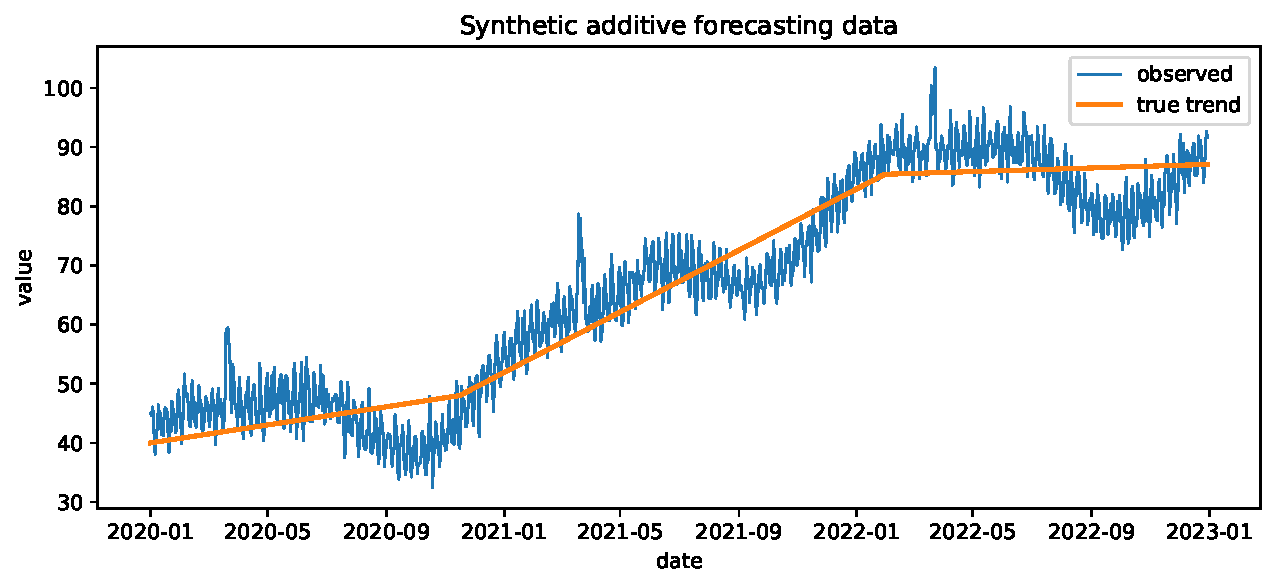
\includegraphics[keepaspectratio]{chapters/chapter-16-automated-forecasting-prophet_files/figure-pdf/ch16-simulate-additive-data-output-1.pdf}}

}

\caption{Synthetic data generated from trend, seasonality, holidays, and
noise.}

\end{figure}%

The data frame uses Prophet-style column names:

\begin{itemize}
\tightlist
\item
  \texttt{ds}: date stamp;
\item
  \texttt{y}: target value.
\end{itemize}

Even if we do not use the Prophet package, this naming convention is
useful because it reminds students that automated forecasting starts
with clean time stamps and a well-defined target.

\section{16.11 Python example: Fourier
features}\label{python-example-fourier-features}

A Fourier seasonal design matrix for period \(P\) and order \(N\) is

\[
X_{\text{season}}(t)=
\left(
\cos\frac{2\pi t}{P},
\sin\frac{2\pi t}{P},
\ldots,
\cos\frac{2\pi Nt}{P},
\sin\frac{2\pi Nt}{P}
\right).
\]

\begin{Shaded}
\begin{Highlighting}[]
\KeywordTok{def}\NormalTok{ fourier\_features(t, period, order, prefix):}
\NormalTok{    t }\OperatorTok{=}\NormalTok{ np.asarray(t)}
\NormalTok{    data }\OperatorTok{=}\NormalTok{ \{\}}
    \ControlFlowTok{for}\NormalTok{ k }\KeywordTok{in} \BuiltInTok{range}\NormalTok{(}\DecValTok{1}\NormalTok{, order }\OperatorTok{+} \DecValTok{1}\NormalTok{):}
\NormalTok{        data[}\SpecialStringTok{f"}\SpecialCharTok{\{}\NormalTok{prefix}\SpecialCharTok{\}}\SpecialStringTok{\_cos\_}\SpecialCharTok{\{}\NormalTok{k}\SpecialCharTok{\}}\SpecialStringTok{"}\NormalTok{] }\OperatorTok{=}\NormalTok{ np.cos(}\DecValTok{2} \OperatorTok{*}\NormalTok{ np.pi }\OperatorTok{*}\NormalTok{ k }\OperatorTok{*}\NormalTok{ t }\OperatorTok{/}\NormalTok{ period)}
\NormalTok{        data[}\SpecialStringTok{f"}\SpecialCharTok{\{}\NormalTok{prefix}\SpecialCharTok{\}}\SpecialStringTok{\_sin\_}\SpecialCharTok{\{}\NormalTok{k}\SpecialCharTok{\}}\SpecialStringTok{"}\NormalTok{] }\OperatorTok{=}\NormalTok{ np.sin(}\DecValTok{2} \OperatorTok{*}\NormalTok{ np.pi }\OperatorTok{*}\NormalTok{ k }\OperatorTok{*}\NormalTok{ t }\OperatorTok{/}\NormalTok{ period)}
    \ControlFlowTok{return}\NormalTok{ pd.DataFrame(data)}

\NormalTok{weekly\_X }\OperatorTok{=}\NormalTok{ fourier\_features(df[}\StringTok{"t"}\NormalTok{], period}\OperatorTok{=}\DecValTok{7}\NormalTok{, order}\OperatorTok{=}\DecValTok{3}\NormalTok{, prefix}\OperatorTok{=}\StringTok{"weekly"}\NormalTok{)}
\NormalTok{weekly\_X.head()}
\end{Highlighting}
\end{Shaded}

\protect\phantomsection\label{ch16-fourier-features}
{\def\LTcaptype{none} % do not increment counter
\begin{longtable}[]{@{}lllllll@{}}
\toprule\noalign{}
& weekly\_cos\_1 & weekly\_sin\_1 & weekly\_cos\_2 & weekly\_sin\_2 &
weekly\_cos\_3 & weekly\_sin\_3 \\
\midrule\noalign{}
\endhead
\bottomrule\noalign{}
\endlastfoot
0 & 1.000000 & 0.000000 & 1.000000 & 0.000000 & 1.000000 & 0.000000 \\
1 & 0.623490 & 0.781831 & -0.222521 & 0.974928 & -0.900969 & 0.433884 \\
2 & -0.222521 & 0.974928 & -0.900969 & -0.433884 & 0.623490 &
-0.781831 \\
3 & -0.900969 & 0.433884 & 0.623490 & -0.781831 & -0.222521 &
0.974928 \\
4 & -0.900969 & -0.433884 & 0.623490 & 0.781831 & -0.222521 &
-0.974928 \\
\end{longtable}
}

Fourier basis functions for weekly seasonality.

\begin{Shaded}
\begin{Highlighting}[]
\NormalTok{fig, ax }\OperatorTok{=}\NormalTok{ plt.subplots(figsize}\OperatorTok{=}\NormalTok{(}\DecValTok{9}\NormalTok{, }\FloatTok{3.5}\NormalTok{))}
\ControlFlowTok{for}\NormalTok{ col }\KeywordTok{in}\NormalTok{ weekly\_X.columns[:}\DecValTok{4}\NormalTok{]:}
\NormalTok{    ax.plot(df[}\StringTok{"t"}\NormalTok{].iloc[:}\DecValTok{28}\NormalTok{], weekly\_X[col].iloc[:}\DecValTok{28}\NormalTok{], label}\OperatorTok{=}\NormalTok{col)}
\NormalTok{ax.set\_title(}\StringTok{"First weekly Fourier basis functions"}\NormalTok{)}
\NormalTok{ax.set\_xlabel(}\StringTok{"time index"}\NormalTok{)}
\NormalTok{ax.legend(ncol}\OperatorTok{=}\DecValTok{2}\NormalTok{)}
\NormalTok{plt.show()}
\end{Highlighting}
\end{Shaded}

\pandocbounded{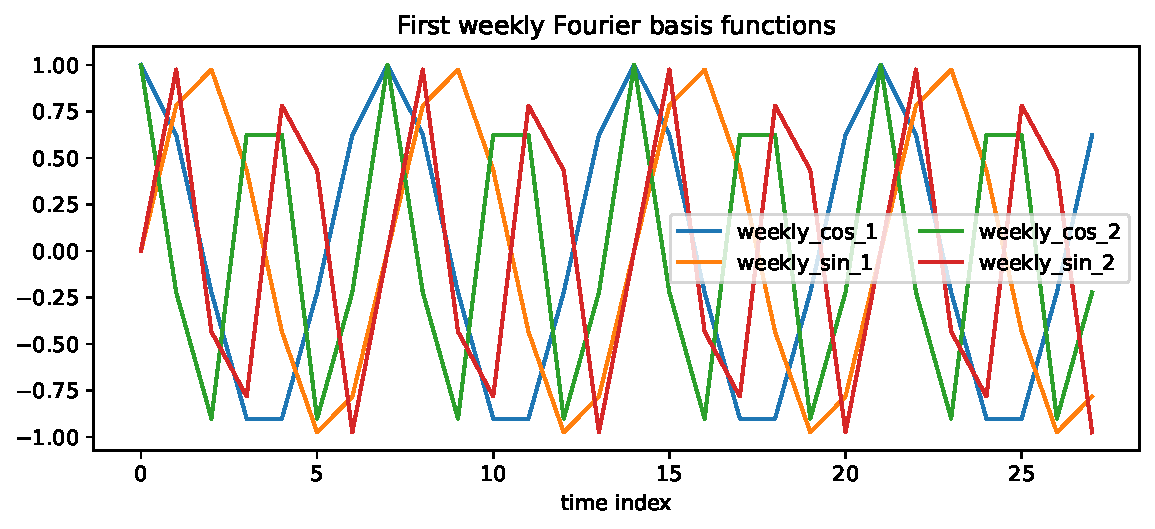
\includegraphics[keepaspectratio]{chapters/chapter-16-automated-forecasting-prophet_files/figure-pdf/ch16-plot-fourier-basis-output-1.pdf}}

Increasing the Fourier order increases flexibility. This is helpful when
the seasonal shape is complex, but too many terms can fit noise.

\section{16.12 Python example: a simplified Prophet-like
regression}\label{python-example-a-simplified-prophet-like-regression}

We can build a Prophet-like model from scratch using:

\begin{enumerate}
\def\labelenumi{\arabic{enumi}.}
\tightlist
\item
  intercept and linear trend;
\item
  hinge functions for changepoints;
\item
  Fourier features for weekly and yearly seasonality;
\item
  holiday indicators;
\item
  ridge regularization.
\end{enumerate}

For clarity, we use a closed-form ridge estimator:

\[
\widehat\beta_{\lambda}
=(X^TX+\lambda I)^{-1}X^Ty.
\]

We usually do not penalize the intercept; below we set the intercept
penalty to zero.

\begin{Shaded}
\begin{Highlighting}[]
\ImportTok{from}\NormalTok{ numpy.linalg }\ImportTok{import}\NormalTok{ solve}

\KeywordTok{def}\NormalTok{ make\_design\_matrix(dates, t, changepoints, weekly\_order}\OperatorTok{=}\DecValTok{3}\NormalTok{, yearly\_order}\OperatorTok{=}\DecValTok{5}\NormalTok{, holiday\_days}\OperatorTok{=}\VariableTok{None}\NormalTok{):}
\NormalTok{    t }\OperatorTok{=}\NormalTok{ np.asarray(t)}
\NormalTok{    parts }\OperatorTok{=}\NormalTok{ []}

    \CommentTok{\# Intercept and linear trend}
\NormalTok{    base }\OperatorTok{=}\NormalTok{ pd.DataFrame(\{}
        \StringTok{"intercept"}\NormalTok{: np.ones\_like(t, dtype}\OperatorTok{=}\BuiltInTok{float}\NormalTok{),}
        \StringTok{"linear\_t"}\NormalTok{: t.astype(}\BuiltInTok{float}\NormalTok{)}
\NormalTok{    \})}
\NormalTok{    parts.append(base)}

    \CommentTok{\# Hinge functions for changepoints}
\NormalTok{    cp\_data }\OperatorTok{=}\NormalTok{ \{\}}
    \ControlFlowTok{for}\NormalTok{ cp }\KeywordTok{in}\NormalTok{ changepoints:}
\NormalTok{        cp\_data[}\SpecialStringTok{f"hinge\_}\SpecialCharTok{\{}\NormalTok{cp}\SpecialCharTok{\}}\SpecialStringTok{"}\NormalTok{] }\OperatorTok{=}\NormalTok{ np.maximum(t }\OperatorTok{{-}}\NormalTok{ cp, }\DecValTok{0}\NormalTok{)}
\NormalTok{    parts.append(pd.DataFrame(cp\_data))}

    \CommentTok{\# Seasonal Fourier features}
\NormalTok{    parts.append(fourier\_features(t, period}\OperatorTok{=}\DecValTok{7}\NormalTok{, order}\OperatorTok{=}\NormalTok{weekly\_order, prefix}\OperatorTok{=}\StringTok{"weekly"}\NormalTok{))}
\NormalTok{    parts.append(fourier\_features(t, period}\OperatorTok{=}\FloatTok{365.25}\NormalTok{, order}\OperatorTok{=}\NormalTok{yearly\_order, prefix}\OperatorTok{=}\StringTok{"yearly"}\NormalTok{))}

    \CommentTok{\# Holiday indicators, with a small window around each event}
    \ControlFlowTok{if}\NormalTok{ holiday\_days }\KeywordTok{is} \KeywordTok{not} \VariableTok{None}\NormalTok{:}
\NormalTok{        h }\OperatorTok{=}\NormalTok{ np.zeros\_like(t, dtype}\OperatorTok{=}\BuiltInTok{float}\NormalTok{)}
        \ControlFlowTok{for}\NormalTok{ day }\KeywordTok{in}\NormalTok{ holiday\_days:}
\NormalTok{            h[np.}\BuiltInTok{abs}\NormalTok{(t }\OperatorTok{{-}}\NormalTok{ day) }\OperatorTok{\textless{}=} \DecValTok{2}\NormalTok{] }\OperatorTok{=} \FloatTok{1.0}
\NormalTok{        parts.append(pd.DataFrame(\{}\StringTok{"holiday\_window"}\NormalTok{: h\}))}

\NormalTok{    X }\OperatorTok{=}\NormalTok{ pd.concat(parts, axis}\OperatorTok{=}\DecValTok{1}\NormalTok{)}
    \ControlFlowTok{return}\NormalTok{ X}

\NormalTok{changepoints }\OperatorTok{=}\NormalTok{ [}\DecValTok{180}\NormalTok{, }\DecValTok{320}\NormalTok{, }\DecValTok{500}\NormalTok{, }\DecValTok{760}\NormalTok{, }\DecValTok{900}\NormalTok{]}
\NormalTok{holiday\_days }\OperatorTok{=}\NormalTok{ [}\DecValTok{80}\NormalTok{, }\DecValTok{445}\NormalTok{, }\DecValTok{810}\NormalTok{]}
\NormalTok{X }\OperatorTok{=}\NormalTok{ make\_design\_matrix(df[}\StringTok{"ds"}\NormalTok{], df[}\StringTok{"t"}\NormalTok{], changepoints, weekly\_order}\OperatorTok{=}\DecValTok{3}\NormalTok{, yearly\_order}\OperatorTok{=}\DecValTok{6}\NormalTok{, holiday\_days}\OperatorTok{=}\NormalTok{holiday\_days)}
\NormalTok{X.head()}
\end{Highlighting}
\end{Shaded}

\protect\phantomsection\label{ch16-build-design-matrix}
{\def\LTcaptype{none} % do not increment counter
\begin{longtable}[]{@{}llllllllllllllllllllll@{}}
\toprule\noalign{}
& intercept & linear\_t & hinge\_180 & hinge\_320 & hinge\_500 &
hinge\_760 & hinge\_900 & weekly\_cos\_1 & weekly\_sin\_1 &
weekly\_cos\_2 & ... & yearly\_sin\_2 & yearly\_cos\_3 & yearly\_sin\_3
& yearly\_cos\_4 & yearly\_sin\_4 & yearly\_cos\_5 & yearly\_sin\_5 &
yearly\_cos\_6 & yearly\_sin\_6 & holiday\_window \\
\midrule\noalign{}
\endhead
\bottomrule\noalign{}
\endlastfoot
0 & 1.0 & 0.0 & 0 & 0 & 0 & 0 & 0 & 1.000000 & 0.000000 & 1.000000 & ...
& 0.000000 & 1.000000 & 0.000000 & 1.000000 & 0.000000 & 1.000000 &
0.000000 & 1.000000 & 0.000000 & 0.0 \\
1 & 1.0 & 1.0 & 0 & 0 & 0 & 0 & 0 & 0.623490 & 0.781831 & -0.222521 &
... & 0.034398 & 0.998669 & 0.051584 & 0.997634 & 0.068755 & 0.996303 &
0.085906 & 0.994678 & 0.103031 & 0.0 \\
2 & 1.0 & 2.0 & 0 & 0 & 0 & 0 & 0 & -0.222521 & 0.974928 & -0.900969 &
... & 0.068755 & 0.994678 & 0.103031 & 0.990545 & 0.137185 & 0.985240 &
0.171177 & 0.978769 & 0.204966 & 0.0 \\
3 & 1.0 & 3.0 & 0 & 0 & 0 & 0 & 0 & -0.900969 & 0.433884 & 0.623490 &
... & 0.103031 & 0.988039 & 0.154204 & 0.978769 & 0.204966 & 0.966893 &
0.255182 & 0.952442 & 0.304719 & 0.0 \\
4 & 1.0 & 4.0 & 0 & 0 & 0 & 0 & 0 & -0.900969 & -0.433884 & 0.623490 &
... & 0.137185 & 0.978769 & 0.204966 & 0.962360 & 0.271777 & 0.941397 &
0.337301 & 0.915978 & 0.401229 & 0.0 \\
\end{longtable}
}

\protect\phantomsection\label{ch16-fit-ridge-prophet-like}
\begin{Shaded}
\begin{Highlighting}[]
\CommentTok{\# Standardize non{-}intercept columns for numerical stability.}
\NormalTok{X\_mat }\OperatorTok{=}\NormalTok{ X.to\_numpy(dtype}\OperatorTok{=}\BuiltInTok{float}\NormalTok{)}
\NormalTok{y\_vec }\OperatorTok{=}\NormalTok{ df[}\StringTok{"y"}\NormalTok{].to\_numpy()}

\NormalTok{means }\OperatorTok{=}\NormalTok{ X\_mat.mean(axis}\OperatorTok{=}\DecValTok{0}\NormalTok{)}
\NormalTok{stds }\OperatorTok{=}\NormalTok{ X\_mat.std(axis}\OperatorTok{=}\DecValTok{0}\NormalTok{)}
\NormalTok{means[}\DecValTok{0}\NormalTok{] }\OperatorTok{=} \FloatTok{0.0}
\NormalTok{stds[}\DecValTok{0}\NormalTok{] }\OperatorTok{=} \FloatTok{1.0}
\NormalTok{stds[stds }\OperatorTok{==} \DecValTok{0}\NormalTok{] }\OperatorTok{=} \FloatTok{1.0}
\NormalTok{X\_scaled }\OperatorTok{=}\NormalTok{ (X\_mat }\OperatorTok{{-}}\NormalTok{ means) }\OperatorTok{/}\NormalTok{ stds}

\NormalTok{lam }\OperatorTok{=} \FloatTok{25.0}
\NormalTok{penalty }\OperatorTok{=}\NormalTok{ np.eye(X\_scaled.shape[}\DecValTok{1}\NormalTok{])}
\NormalTok{penalty[}\DecValTok{0}\NormalTok{, }\DecValTok{0}\NormalTok{] }\OperatorTok{=} \FloatTok{0.0}

\NormalTok{beta }\OperatorTok{=}\NormalTok{ solve(X\_scaled.T }\OperatorTok{@}\NormalTok{ X\_scaled }\OperatorTok{+}\NormalTok{ lam }\OperatorTok{*}\NormalTok{ penalty, X\_scaled.T }\OperatorTok{@}\NormalTok{ y\_vec)}
\NormalTok{yhat }\OperatorTok{=}\NormalTok{ X\_scaled }\OperatorTok{@}\NormalTok{ beta}

\NormalTok{rmse }\OperatorTok{=}\NormalTok{ np.sqrt(np.mean((y\_vec }\OperatorTok{{-}}\NormalTok{ yhat) }\OperatorTok{**} \DecValTok{2}\NormalTok{))}
\NormalTok{mae }\OperatorTok{=}\NormalTok{ np.mean(np.}\BuiltInTok{abs}\NormalTok{(y\_vec }\OperatorTok{{-}}\NormalTok{ yhat))}
\BuiltInTok{print}\NormalTok{(}\SpecialStringTok{f"In{-}sample RMSE: }\SpecialCharTok{\{}\NormalTok{rmse}\SpecialCharTok{:.3f\}}\SpecialStringTok{"}\NormalTok{)}
\BuiltInTok{print}\NormalTok{(}\SpecialStringTok{f"In{-}sample MAE:  }\SpecialCharTok{\{}\NormalTok{mae}\SpecialCharTok{:.3f\}}\SpecialStringTok{"}\NormalTok{)}
\end{Highlighting}
\end{Shaded}

\begin{verbatim}
In-sample RMSE: 2.162
In-sample MAE:  1.742
\end{verbatim}

\begin{Shaded}
\begin{Highlighting}[]
\NormalTok{fig, ax }\OperatorTok{=}\NormalTok{ plt.subplots(figsize}\OperatorTok{=}\NormalTok{(}\DecValTok{10}\NormalTok{, }\DecValTok{4}\NormalTok{))}
\NormalTok{ax.plot(df[}\StringTok{"ds"}\NormalTok{], df[}\StringTok{"y"}\NormalTok{], linewidth}\OperatorTok{=}\DecValTok{1}\NormalTok{, label}\OperatorTok{=}\StringTok{"observed"}\NormalTok{)}
\NormalTok{ax.plot(df[}\StringTok{"ds"}\NormalTok{], yhat, linewidth}\OperatorTok{=}\DecValTok{2}\NormalTok{, label}\OperatorTok{=}\StringTok{"fitted additive model"}\NormalTok{)}
\NormalTok{ax.set\_title(}\StringTok{"Prophet{-}like additive regression fit"}\NormalTok{)}
\NormalTok{ax.set\_xlabel(}\StringTok{"date"}\NormalTok{)}
\NormalTok{ax.set\_ylabel(}\StringTok{"value"}\NormalTok{)}
\NormalTok{ax.legend()}
\NormalTok{plt.show()}
\end{Highlighting}
\end{Shaded}

\begin{figure}[H]

{\centering \pandocbounded{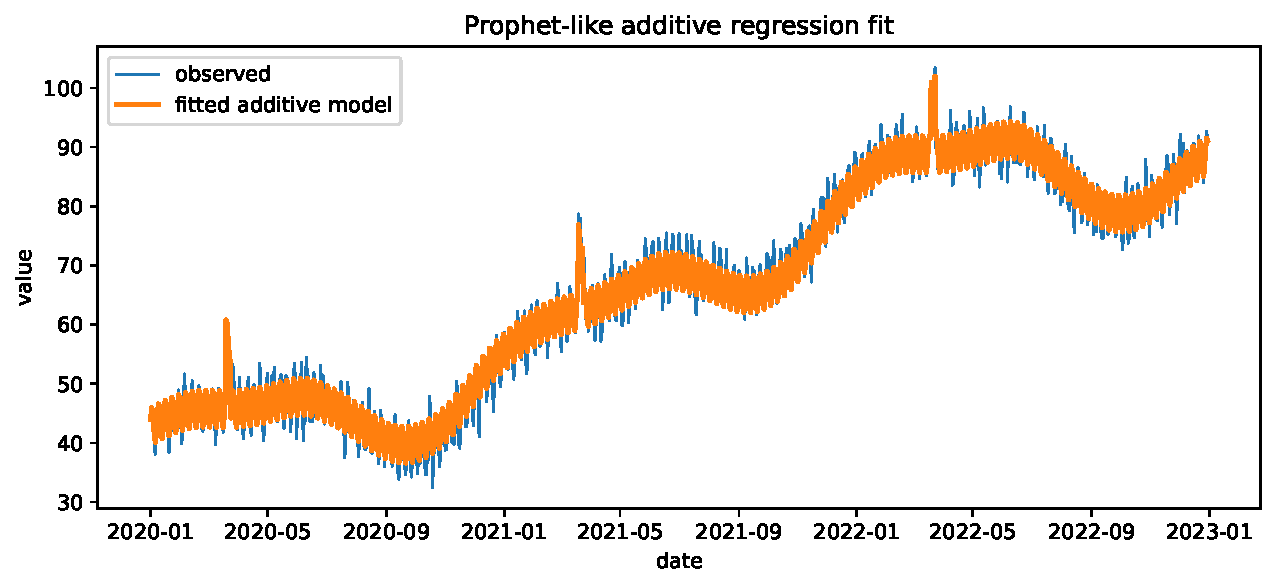
\includegraphics[keepaspectratio]{chapters/chapter-16-automated-forecasting-prophet_files/figure-pdf/ch16-plot-fit-output-1.pdf}}

}

\caption{Simplified Prophet-like regression fit.}

\end{figure}%

This is not the full Prophet algorithm, but it captures the mathematical
structure students should understand: basis expansion plus regularized
estimation.

\section{16.13 Forecasting future dates}\label{forecasting-future-dates}

To forecast future dates, we create the same features for future time
indices and multiply by the fitted coefficient vector.

\begin{Shaded}
\begin{Highlighting}[]
\NormalTok{h }\OperatorTok{=} \DecValTok{120}
\NormalTok{future\_dates }\OperatorTok{=}\NormalTok{ pd.date\_range(df[}\StringTok{"ds"}\NormalTok{].iloc[}\OperatorTok{{-}}\DecValTok{1}\NormalTok{] }\OperatorTok{+}\NormalTok{ pd.Timedelta(days}\OperatorTok{=}\DecValTok{1}\NormalTok{), periods}\OperatorTok{=}\NormalTok{h, freq}\OperatorTok{=}\StringTok{"D"}\NormalTok{)}
\NormalTok{future\_t }\OperatorTok{=}\NormalTok{ np.arange(n, n }\OperatorTok{+}\NormalTok{ h)}

\NormalTok{future\_X }\OperatorTok{=}\NormalTok{ make\_design\_matrix(}
\NormalTok{    future\_dates,}
\NormalTok{    future\_t,}
\NormalTok{    changepoints}\OperatorTok{=}\NormalTok{changepoints,}
\NormalTok{    weekly\_order}\OperatorTok{=}\DecValTok{3}\NormalTok{,}
\NormalTok{    yearly\_order}\OperatorTok{=}\DecValTok{6}\NormalTok{,}
\NormalTok{    holiday\_days}\OperatorTok{=}\NormalTok{holiday\_days }\OperatorTok{+}\NormalTok{ [}\DecValTok{1175}\NormalTok{]  }\CommentTok{\# an assumed future holiday/event}
\NormalTok{)}

\NormalTok{future\_mat }\OperatorTok{=}\NormalTok{ future\_X.to\_numpy(dtype}\OperatorTok{=}\BuiltInTok{float}\NormalTok{)}
\NormalTok{future\_scaled }\OperatorTok{=}\NormalTok{ (future\_mat }\OperatorTok{{-}}\NormalTok{ means) }\OperatorTok{/}\NormalTok{ stds}
\NormalTok{future\_yhat }\OperatorTok{=}\NormalTok{ future\_scaled }\OperatorTok{@}\NormalTok{ beta}

\NormalTok{fig, ax }\OperatorTok{=}\NormalTok{ plt.subplots(figsize}\OperatorTok{=}\NormalTok{(}\DecValTok{10}\NormalTok{, }\DecValTok{4}\NormalTok{))}
\NormalTok{ax.plot(df[}\StringTok{"ds"}\NormalTok{].iloc[}\OperatorTok{{-}}\DecValTok{365}\NormalTok{:], df[}\StringTok{"y"}\NormalTok{].iloc[}\OperatorTok{{-}}\DecValTok{365}\NormalTok{:], linewidth}\OperatorTok{=}\DecValTok{1}\NormalTok{, label}\OperatorTok{=}\StringTok{"history"}\NormalTok{)}
\NormalTok{ax.plot(future\_dates, future\_yhat, linewidth}\OperatorTok{=}\DecValTok{2}\NormalTok{, label}\OperatorTok{=}\StringTok{"forecast"}\NormalTok{)}
\NormalTok{ax.axvline(df[}\StringTok{"ds"}\NormalTok{].iloc[}\OperatorTok{{-}}\DecValTok{1}\NormalTok{], linestyle}\OperatorTok{=}\StringTok{"{-}{-}"}\NormalTok{, linewidth}\OperatorTok{=}\DecValTok{1}\NormalTok{)}
\NormalTok{ax.set\_title(}\StringTok{"Forecast from simplified Prophet{-}like model"}\NormalTok{)}
\NormalTok{ax.set\_xlabel(}\StringTok{"date"}\NormalTok{)}
\NormalTok{ax.set\_ylabel(}\StringTok{"value"}\NormalTok{)}
\NormalTok{ax.legend()}
\NormalTok{plt.show()}
\end{Highlighting}
\end{Shaded}

\begin{figure}[H]

{\centering \pandocbounded{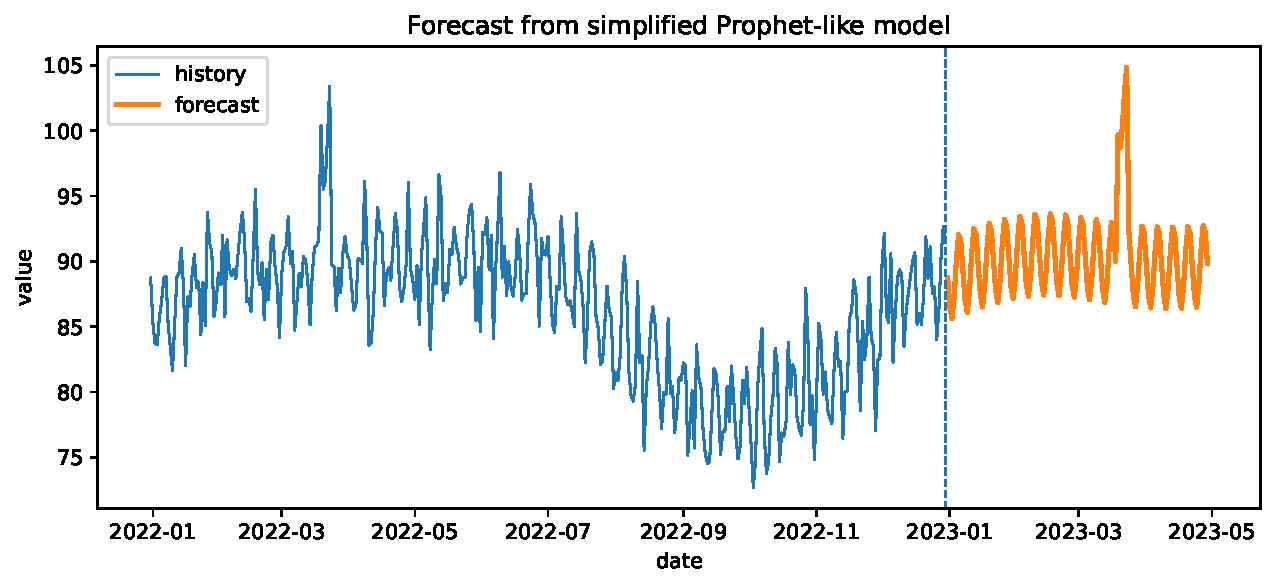
\includegraphics[keepaspectratio]{chapters/chapter-16-automated-forecasting-prophet_files/figure-pdf/ch16-future-forecast-output-1.pdf}}

}

\caption{Future forecast from the simplified additive model.}

\end{figure}%

The forecast extrapolates the final trend slope and repeats seasonal
patterns. This is convenient, but it can be dangerous if the latest
trend slope was caused by a temporary event.

\section{16.14 Cross-validation for automated
forecasting}\label{cross-validation-for-automated-forecasting}

Prophet popularized an analyst-friendly cross-validation interface with
three key quantities:

\begin{itemize}
\tightlist
\item
  \textbf{initial}: length of the first training window;
\item
  \textbf{period}: spacing between forecast cutoffs;
\item
  \textbf{horizon}: forecast horizon.
\end{itemize}

For cutoffs \(c_1,c_2,\ldots,c_M\), the model is trained using data up
to cutoff \(c_m\) and predicts

\[
y(c_m+1),\ldots,y(c_m+H).
\]

The evaluation table contains rows of the form

\[
(c_m,h,y_{c_m+h},\widehat y_{c_m+h\mid c_m}).
\]

Then scores can be summarized by horizon.

\begin{Shaded}
\begin{Highlighting}[]
\KeywordTok{def}\NormalTok{ fit\_ridge\_additive(train\_df, changepoints, weekly\_order, yearly\_order, holiday\_days, lam}\OperatorTok{=}\FloatTok{25.0}\NormalTok{):}
\NormalTok{    X\_train }\OperatorTok{=}\NormalTok{ make\_design\_matrix(}
\NormalTok{        train\_df[}\StringTok{"ds"}\NormalTok{], train\_df[}\StringTok{"t"}\NormalTok{], changepoints,}
\NormalTok{        weekly\_order}\OperatorTok{=}\NormalTok{weekly\_order,}
\NormalTok{        yearly\_order}\OperatorTok{=}\NormalTok{yearly\_order,}
\NormalTok{        holiday\_days}\OperatorTok{=}\NormalTok{holiday\_days}
\NormalTok{    )}
\NormalTok{    X\_mat }\OperatorTok{=}\NormalTok{ X\_train.to\_numpy(dtype}\OperatorTok{=}\BuiltInTok{float}\NormalTok{)}
\NormalTok{    y\_train }\OperatorTok{=}\NormalTok{ train\_df[}\StringTok{"y"}\NormalTok{].to\_numpy()}

\NormalTok{    means }\OperatorTok{=}\NormalTok{ X\_mat.mean(axis}\OperatorTok{=}\DecValTok{0}\NormalTok{)}
\NormalTok{    stds }\OperatorTok{=}\NormalTok{ X\_mat.std(axis}\OperatorTok{=}\DecValTok{0}\NormalTok{)}
\NormalTok{    means[}\DecValTok{0}\NormalTok{] }\OperatorTok{=} \FloatTok{0.0}
\NormalTok{    stds[}\DecValTok{0}\NormalTok{] }\OperatorTok{=} \FloatTok{1.0}
\NormalTok{    stds[stds }\OperatorTok{==} \DecValTok{0}\NormalTok{] }\OperatorTok{=} \FloatTok{1.0}
\NormalTok{    X\_scaled }\OperatorTok{=}\NormalTok{ (X\_mat }\OperatorTok{{-}}\NormalTok{ means) }\OperatorTok{/}\NormalTok{ stds}

\NormalTok{    penalty }\OperatorTok{=}\NormalTok{ np.eye(X\_scaled.shape[}\DecValTok{1}\NormalTok{])}
\NormalTok{    penalty[}\DecValTok{0}\NormalTok{, }\DecValTok{0}\NormalTok{] }\OperatorTok{=} \FloatTok{0.0}
\NormalTok{    beta }\OperatorTok{=}\NormalTok{ solve(X\_scaled.T }\OperatorTok{@}\NormalTok{ X\_scaled }\OperatorTok{+}\NormalTok{ lam }\OperatorTok{*}\NormalTok{ penalty, X\_scaled.T }\OperatorTok{@}\NormalTok{ y\_train)}
    \ControlFlowTok{return}\NormalTok{ beta, means, stds, X\_train.columns}


\KeywordTok{def}\NormalTok{ predict\_ridge\_additive(test\_df, beta, means, stds, changepoints, weekly\_order, yearly\_order, holiday\_days):}
\NormalTok{    X\_test }\OperatorTok{=}\NormalTok{ make\_design\_matrix(}
\NormalTok{        test\_df[}\StringTok{"ds"}\NormalTok{], test\_df[}\StringTok{"t"}\NormalTok{], changepoints,}
\NormalTok{        weekly\_order}\OperatorTok{=}\NormalTok{weekly\_order,}
\NormalTok{        yearly\_order}\OperatorTok{=}\NormalTok{yearly\_order,}
\NormalTok{        holiday\_days}\OperatorTok{=}\NormalTok{holiday\_days}
\NormalTok{    )}
\NormalTok{    X\_mat }\OperatorTok{=}\NormalTok{ X\_test.to\_numpy(dtype}\OperatorTok{=}\BuiltInTok{float}\NormalTok{)}
\NormalTok{    X\_scaled }\OperatorTok{=}\NormalTok{ (X\_mat }\OperatorTok{{-}}\NormalTok{ means) }\OperatorTok{/}\NormalTok{ stds}
    \ControlFlowTok{return}\NormalTok{ X\_scaled }\OperatorTok{@}\NormalTok{ beta}

\NormalTok{horizon }\OperatorTok{=} \DecValTok{60}
\NormalTok{initial }\OperatorTok{=} \DecValTok{2} \OperatorTok{*} \DecValTok{365}
\NormalTok{period }\OperatorTok{=} \DecValTok{90}
\NormalTok{cutoffs }\OperatorTok{=} \BuiltInTok{list}\NormalTok{(}\BuiltInTok{range}\NormalTok{(initial, n }\OperatorTok{{-}}\NormalTok{ horizon, period))}

\NormalTok{records }\OperatorTok{=}\NormalTok{ []}
\ControlFlowTok{for}\NormalTok{ cutoff }\KeywordTok{in}\NormalTok{ cutoffs:}
\NormalTok{    train\_df }\OperatorTok{=}\NormalTok{ df.iloc[:cutoff].copy()}
\NormalTok{    test\_df }\OperatorTok{=}\NormalTok{ df.iloc[cutoff:cutoff }\OperatorTok{+}\NormalTok{ horizon].copy()}

\NormalTok{    beta\_cv, means\_cv, stds\_cv, \_ }\OperatorTok{=}\NormalTok{ fit\_ridge\_additive(}
\NormalTok{        train\_df, changepoints}\OperatorTok{=}\NormalTok{[}\DecValTok{180}\NormalTok{, }\DecValTok{320}\NormalTok{, }\DecValTok{500}\NormalTok{, }\DecValTok{760}\NormalTok{],}
\NormalTok{        weekly\_order}\OperatorTok{=}\DecValTok{3}\NormalTok{, yearly\_order}\OperatorTok{=}\DecValTok{6}\NormalTok{,}
\NormalTok{        holiday\_days}\OperatorTok{=}\NormalTok{holiday\_days,}
\NormalTok{        lam}\OperatorTok{=}\FloatTok{25.0}
\NormalTok{    )}
\NormalTok{    pred }\OperatorTok{=}\NormalTok{ predict\_ridge\_additive(}
\NormalTok{        test\_df, beta\_cv, means\_cv, stds\_cv,}
\NormalTok{        changepoints}\OperatorTok{=}\NormalTok{[}\DecValTok{180}\NormalTok{, }\DecValTok{320}\NormalTok{, }\DecValTok{500}\NormalTok{, }\DecValTok{760}\NormalTok{],}
\NormalTok{        weekly\_order}\OperatorTok{=}\DecValTok{3}\NormalTok{, yearly\_order}\OperatorTok{=}\DecValTok{6}\NormalTok{,}
\NormalTok{        holiday\_days}\OperatorTok{=}\NormalTok{holiday\_days}
\NormalTok{    )}

    \ControlFlowTok{for}\NormalTok{ h\_i, (actual, forecast) }\KeywordTok{in} \BuiltInTok{enumerate}\NormalTok{(}\BuiltInTok{zip}\NormalTok{(test\_df[}\StringTok{"y"}\NormalTok{].to\_numpy(), pred), start}\OperatorTok{=}\DecValTok{1}\NormalTok{):}
\NormalTok{        records.append(\{}
            \StringTok{"cutoff"}\NormalTok{: cutoff,}
            \StringTok{"horizon"}\NormalTok{: h\_i,}
            \StringTok{"y"}\NormalTok{: actual,}
            \StringTok{"yhat"}\NormalTok{: forecast,}
            \StringTok{"error"}\NormalTok{: actual }\OperatorTok{{-}}\NormalTok{ forecast,}
            \StringTok{"abs\_error"}\NormalTok{: }\BuiltInTok{abs}\NormalTok{(actual }\OperatorTok{{-}}\NormalTok{ forecast)}
\NormalTok{        \})}

\NormalTok{cv }\OperatorTok{=}\NormalTok{ pd.DataFrame(records)}
\NormalTok{mae\_by\_h }\OperatorTok{=}\NormalTok{ cv.groupby(}\StringTok{"horizon"}\NormalTok{)[}\StringTok{"abs\_error"}\NormalTok{].mean()}

\NormalTok{fig, ax }\OperatorTok{=}\NormalTok{ plt.subplots(figsize}\OperatorTok{=}\NormalTok{(}\DecValTok{8}\NormalTok{, }\FloatTok{3.5}\NormalTok{))}
\NormalTok{ax.plot(mae\_by\_h.index, mae\_by\_h.values)}
\NormalTok{ax.set\_title(}\StringTok{"Cross{-}validation MAE by horizon"}\NormalTok{)}
\NormalTok{ax.set\_xlabel(}\StringTok{"forecast horizon"}\NormalTok{)}
\NormalTok{ax.set\_ylabel(}\StringTok{"MAE"}\NormalTok{)}
\NormalTok{plt.show()}
\end{Highlighting}
\end{Shaded}

\begin{figure}[H]

{\centering \pandocbounded{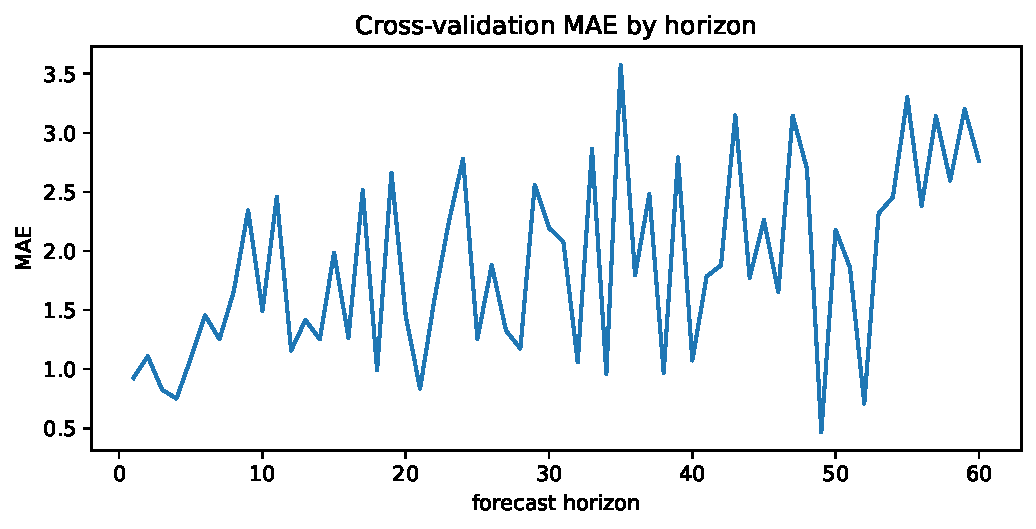
\includegraphics[keepaspectratio]{chapters/chapter-16-automated-forecasting-prophet_files/figure-pdf/ch16-rolling-origin-cv-output-1.pdf}}

}

\caption{Rolling-origin cross-validation errors by horizon.}

\end{figure}%

Averaging over horizons can hide systematic deterioration. Horizon-wise
plots are often more informative than one number.

\section{16.15 Forecast metrics in automated
workflows}\label{forecast-metrics-in-automated-workflows}

Chapter 15 introduced several metrics. Automated forecasting pipelines
often report:

\subsection{Absolute and squared
error}\label{absolute-and-squared-error}

\[
\operatorname{MAE}=\frac{1}{n}\sum_{i=1}^n|y_i-\widehat y_i|,
\]

\[
\operatorname{RMSE}=\sqrt{\frac{1}{n}\sum_{i=1}^n(y_i-\widehat y_i)^2}.
\]

MAE is robust and easy to interpret. RMSE penalizes large errors more
strongly.

\subsection{Percent error}\label{percent-error}

\[
\operatorname{MAPE}
=\frac{100}{n}\sum_{i=1}^n
\left|\frac{y_i-\widehat y_i}{y_i}\right|.
\]

MAPE is easy to communicate, but it fails when \(y_i=0\) and behaves
poorly when \(y_i\) is near zero.

\subsection{Scaled error}\label{scaled-error}

A scaled error compares the model to a baseline. For seasonal period
\(s\), the mean absolute scaled error is

\[
\operatorname{MASE}
=\frac{\frac{1}{n}\sum_{i=1}^n|y_i-\widehat y_i|}
{\frac{1}{T-s}\sum_{t=s+1}^T |y_t-y_{t-s}|}.
\]

A MASE below \(1\) means the model improves over the seasonal naive
baseline.

\subsection{Relative error}\label{relative-error}

A relative error compares directly to a benchmark forecast:

\[
\operatorname{RelMAE}
=\frac{\operatorname{MAE}(\text{model})}
{\operatorname{MAE}(\text{benchmark})}.
\]

This is useful at scale because raw MAE values are not comparable across
series with different units and scales.

\begin{tcolorbox}[enhanced jigsaw, arc=.35mm, bottomrule=.15mm, bottomtitle=1mm, breakable, colback=white, colbacktitle=quarto-callout-tip-color!10!white, colframe=quarto-callout-tip-color-frame, coltitle=black, left=2mm, leftrule=.75mm, opacityback=0, opacitybacktitle=0.6, rightrule=.15mm, title=\textcolor{quarto-callout-tip-color}{\faLightbulb}\hspace{0.5em}{Use benchmark-relative metrics}, titlerule=0mm, toprule=.15mm, toptitle=1mm]

When reporting many automated forecasts, include a baseline-relative
metric such as MASE or relative MAE. A raw MAPE of \(5\%\) may be
excellent for one series and poor for another.

\end{tcolorbox}

\section{16.16 Hyperparameter tuning}\label{hyperparameter-tuning}

Important Prophet-type tuning parameters include:

\begin{enumerate}
\def\labelenumi{\arabic{enumi}.}
\tightlist
\item
  \textbf{changepoint flexibility}: controls how much the trend can
  bend;
\item
  \textbf{seasonality flexibility}: controls the size and smoothness of
  seasonal effects;
\item
  \textbf{holiday flexibility}: controls how strongly holiday effects
  are allowed to move the forecast;
\item
  \textbf{seasonality mode}: additive or multiplicative;
\item
  \textbf{Fourier order}: number of Fourier terms for each seasonal
  period;
\item
  \textbf{changepoint range}: portion of history where changepoints are
  allowed.
\end{enumerate}

Hyperparameter tuning should be done by time-aware cross-validation. A
generic procedure is:

\begin{enumerate}
\def\labelenumi{\arabic{enumi}.}
\tightlist
\item
  choose a grid of candidate parameters;
\item
  for each parameter combination, run rolling-origin cross-validation;
\item
  compute horizon-wise and aggregate metrics;
\item
  choose a parameter set using validation performance and model
  simplicity;
\item
  refit the selected model on all available training data;
\item
  evaluate once on a final untouched test set, if available.
\end{enumerate}

\begin{Shaded}
\begin{Highlighting}[]
\CommentTok{\# A small demonstration grid over Fourier order and ridge penalty.}
\CommentTok{\# For speed, this example uses a short grid.}
\NormalTok{grid }\OperatorTok{=}\NormalTok{ []}
\ControlFlowTok{for}\NormalTok{ yearly\_order }\KeywordTok{in}\NormalTok{ [}\DecValTok{3}\NormalTok{, }\DecValTok{6}\NormalTok{, }\DecValTok{10}\NormalTok{]:}
    \ControlFlowTok{for}\NormalTok{ lam }\KeywordTok{in}\NormalTok{ [}\FloatTok{5.0}\NormalTok{, }\FloatTok{25.0}\NormalTok{, }\FloatTok{100.0}\NormalTok{]:}
\NormalTok{        records }\OperatorTok{=}\NormalTok{ []}
        \ControlFlowTok{for}\NormalTok{ cutoff }\KeywordTok{in}\NormalTok{ cutoffs:}
\NormalTok{            train\_df }\OperatorTok{=}\NormalTok{ df.iloc[:cutoff].copy()}
\NormalTok{            test\_df }\OperatorTok{=}\NormalTok{ df.iloc[cutoff:cutoff }\OperatorTok{+}\NormalTok{ horizon].copy()}
\NormalTok{            beta\_cv, means\_cv, stds\_cv, \_ }\OperatorTok{=}\NormalTok{ fit\_ridge\_additive(}
\NormalTok{                train\_df, changepoints}\OperatorTok{=}\NormalTok{[}\DecValTok{180}\NormalTok{, }\DecValTok{320}\NormalTok{, }\DecValTok{500}\NormalTok{, }\DecValTok{760}\NormalTok{],}
\NormalTok{                weekly\_order}\OperatorTok{=}\DecValTok{3}\NormalTok{, yearly\_order}\OperatorTok{=}\NormalTok{yearly\_order,}
\NormalTok{                holiday\_days}\OperatorTok{=}\NormalTok{holiday\_days,}
\NormalTok{                lam}\OperatorTok{=}\NormalTok{lam}
\NormalTok{            )}
\NormalTok{            pred }\OperatorTok{=}\NormalTok{ predict\_ridge\_additive(}
\NormalTok{                test\_df, beta\_cv, means\_cv, stds\_cv,}
\NormalTok{                changepoints}\OperatorTok{=}\NormalTok{[}\DecValTok{180}\NormalTok{, }\DecValTok{320}\NormalTok{, }\DecValTok{500}\NormalTok{, }\DecValTok{760}\NormalTok{],}
\NormalTok{                weekly\_order}\OperatorTok{=}\DecValTok{3}\NormalTok{, yearly\_order}\OperatorTok{=}\NormalTok{yearly\_order,}
\NormalTok{                holiday\_days}\OperatorTok{=}\NormalTok{holiday\_days}
\NormalTok{            )}
\NormalTok{            records.extend(np.}\BuiltInTok{abs}\NormalTok{(test\_df[}\StringTok{"y"}\NormalTok{].to\_numpy() }\OperatorTok{{-}}\NormalTok{ pred))}
\NormalTok{        grid.append(\{}\StringTok{"yearly\_order"}\NormalTok{: yearly\_order, }\StringTok{"lambda"}\NormalTok{: lam, }\StringTok{"cv\_mae"}\NormalTok{: }\BuiltInTok{float}\NormalTok{(np.mean(records))\})}

\NormalTok{grid\_results }\OperatorTok{=}\NormalTok{ pd.DataFrame(grid).sort\_values(}\StringTok{"cv\_mae"}\NormalTok{)}
\NormalTok{grid\_results}
\end{Highlighting}
\end{Shaded}

\protect\phantomsection\label{ch16-small-grid-search}
{\def\LTcaptype{none} % do not increment counter
\begin{longtable}[]{@{}llll@{}}
\toprule\noalign{}
& yearly\_order & lambda & cv\_mae \\
\midrule\noalign{}
\endhead
\bottomrule\noalign{}
\endlastfoot
1 & 3 & 25.0 & 1.876340 \\
4 & 6 & 25.0 & 1.887394 \\
7 & 10 & 25.0 & 1.932436 \\
0 & 3 & 5.0 & 2.002318 \\
3 & 6 & 5.0 & 2.051687 \\
6 & 10 & 5.0 & 2.098388 \\
5 & 6 & 100.0 & 2.720480 \\
8 & 10 & 100.0 & 2.750983 \\
2 & 3 & 100.0 & 2.753779 \\
\end{longtable}
}

This example tunes a simplified model. The same idea applies to real
Prophet parameters such as \texttt{changepoint\_prior\_scale},
\texttt{seasonality\_prior\_scale}, \texttt{holidays\_prior\_scale}, and
\texttt{seasonality\_mode}.

\section{16.17 Optional package example: Prophet
syntax}\label{optional-package-example-prophet-syntax}

The exact package name and installation method may depend on the
computing environment. The following code is provided as a template. It
is not executed by default in this book.

\begin{Shaded}
\begin{Highlighting}[]
\CommentTok{\# Optional template; run only after installing prophet in your environment.}
\ImportTok{from}\NormalTok{ prophet }\ImportTok{import}\NormalTok{ Prophet}
\ImportTok{from}\NormalTok{ prophet.diagnostics }\ImportTok{import}\NormalTok{ cross\_validation, performance\_metrics}
\ImportTok{from}\NormalTok{ prophet.plot }\ImportTok{import}\NormalTok{ plot\_cross\_validation\_metric}

\NormalTok{m }\OperatorTok{=}\NormalTok{ Prophet(}
\NormalTok{    yearly\_seasonality}\OperatorTok{=}\VariableTok{True}\NormalTok{,}
\NormalTok{    weekly\_seasonality}\OperatorTok{=}\VariableTok{True}\NormalTok{,}
\NormalTok{    daily\_seasonality}\OperatorTok{=}\VariableTok{False}\NormalTok{,}
\NormalTok{    seasonality\_mode}\OperatorTok{=}\StringTok{"additive"}\NormalTok{,}
\NormalTok{    changepoint\_prior\_scale}\OperatorTok{=}\FloatTok{0.05}\NormalTok{,}
\NormalTok{    seasonality\_prior\_scale}\OperatorTok{=}\FloatTok{10.0}\NormalTok{,}
\NormalTok{)}

\CommentTok{\# df must have columns ds and y.}
\NormalTok{m.fit(df[[}\StringTok{"ds"}\NormalTok{, }\StringTok{"y"}\NormalTok{]])}

\NormalTok{future }\OperatorTok{=}\NormalTok{ m.make\_future\_dataframe(periods}\OperatorTok{=}\DecValTok{120}\NormalTok{, freq}\OperatorTok{=}\StringTok{"D"}\NormalTok{)}
\NormalTok{forecast }\OperatorTok{=}\NormalTok{ m.predict(future)}

\NormalTok{fig1 }\OperatorTok{=}\NormalTok{ m.plot(forecast)}
\NormalTok{fig2 }\OperatorTok{=}\NormalTok{ m.plot\_components(forecast)}

\CommentTok{\# Rolling{-}origin style cross{-}validation.}
\NormalTok{df\_cv }\OperatorTok{=}\NormalTok{ cross\_validation(}
\NormalTok{    m,}
\NormalTok{    initial}\OperatorTok{=}\StringTok{"730 days"}\NormalTok{,}
\NormalTok{    period}\OperatorTok{=}\StringTok{"180 days"}\NormalTok{,}
\NormalTok{    horizon}\OperatorTok{=}\StringTok{"365 days"}
\NormalTok{)}

\NormalTok{df\_perf }\OperatorTok{=}\NormalTok{ performance\_metrics(df\_cv)}
\NormalTok{fig3 }\OperatorTok{=}\NormalTok{ plot\_cross\_validation\_metric(df\_cv, metric}\OperatorTok{=}\StringTok{"mae"}\NormalTok{)}
\end{Highlighting}
\end{Shaded}

The important conceptual point is not the package call. The important
point is the workflow: clean data, specify components, fit, inspect
decomposition, cross-validate, tune, and compare with baselines.

\section{16.18 Analyst-in-the-loop
modeling}\label{analyst-in-the-loop-modeling}

Prophet-type models are designed for analyst intervention. The analyst
can supply:

\begin{itemize}
\tightlist
\item
  known capacities for logistic growth;
\item
  manually selected changepoints;
\item
  country, institutional, or domain-specific holidays;
\item
  custom seasonalities;
\item
  prior scales controlling smoothness;
\item
  outlier handling decisions;
\item
  external regressors.
\end{itemize}

This is a strength when domain knowledge is reliable. It is a weakness
when analyst choices are not validated.

An analyst-in-the-loop workflow:

\begin{enumerate}
\def\labelenumi{\arabic{enumi}.}
\tightlist
\item
  Fit simple default model.
\item
  Inspect trend, seasonality, holiday components.
\item
  Compare with naive and seasonal naive baselines.
\item
  Check residuals and forecast errors by horizon.
\item
  Add known holidays or events.
\item
  Tune prior scales using rolling-origin cross-validation.
\item
  Refit and communicate the final assumptions.
\end{enumerate}

\section{16.19 Diagnostics and failure
modes}\label{diagnostics-and-failure-modes}

A Prophet-type model can fail for several reasons.

\subsection{Autocorrelated residuals}\label{autocorrelated-residuals}

Because the model is closer to curve fitting than ARIMA, it may leave
serial dependence in residuals. If residual ACF shows strong structure,
consider:

\begin{itemize}
\tightlist
\item
  adding autoregressive features;
\item
  using SARIMA/state-space models;
\item
  using a hybrid model;
\item
  using ML lag features.
\end{itemize}

\subsection{Extrapolation error}\label{extrapolation-error}

Piecewise linear trend extrapolates the final trend regime. If the last
trend segment is temporary, long-range forecasts can be poor.

\subsection{Overfitting changepoints}\label{overfitting-changepoints}

Too much changepoint flexibility can fit noise and create unstable
future trends.

\subsection{Overfitting seasonalities}\label{overfitting-seasonalities}

Large Fourier order can produce unrealistic seasonal wiggles.

\subsection{Bad holiday design}\label{bad-holiday-design}

Too many event indicators can fit random spikes. Missing important
events can leave systematic errors.

\subsection{Multiplicative structure
ignored}\label{multiplicative-structure-ignored}

If variance and seasonal amplitude grow with level, additive errors may
be inappropriate.

\subsection{Irregular data without
context}\label{irregular-data-without-context}

Prophet can handle missing dates better than many ARIMA implementations,
but missingness may still be informative. For example, no sales on a
closed day is different from missing data.

\section{16.20 Comparing Prophet-type models with
SARIMA}\label{comparing-prophet-type-models-with-sarima}

SARIMA and Prophet-type models use different modeling philosophies.

{\def\LTcaptype{none} % do not increment counter
\begin{longtable}[]{@{}
  >{\raggedright\arraybackslash}p{(\linewidth - 4\tabcolsep) * \real{0.3333}}
  >{\raggedright\arraybackslash}p{(\linewidth - 4\tabcolsep) * \real{0.3333}}
  >{\raggedright\arraybackslash}p{(\linewidth - 4\tabcolsep) * \real{0.3333}}@{}}
\toprule\noalign{}
\begin{minipage}[b]{\linewidth}\raggedright
Issue
\end{minipage} & \begin{minipage}[b]{\linewidth}\raggedright
SARIMA
\end{minipage} & \begin{minipage}[b]{\linewidth}\raggedright
Prophet-type additive model
\end{minipage} \\
\midrule\noalign{}
\endhead
\bottomrule\noalign{}
\endlastfoot
Main structure & lag dependence and shocks & trend + seasonality +
events \\
Stationarity & often requires differencing & trend handled directly \\
Seasonality & seasonal lags and seasonal differencing & Fourier seasonal
basis \\
Holidays & not built in by default & natural event indicators \\
Missing dates & can be inconvenient & usually easier \\
Interpretability & AR/MA coefficients and residuals & decomposed
components \\
Residual dependence & modeled directly & may remain unless added \\
Scaling to many series & possible but tuning can be slow & designed for
fast iteration \\
\end{longtable}
}

A practical approach is not to ask, ``Which model is universally
better?'' Instead ask:

\begin{quote}
Which model wins under the actual backtest, forecast horizon, metric,
and operational constraints?
\end{quote}

\section{16.21 AI-assisted automated
forecasting}\label{ai-assisted-automated-forecasting}

AI tools can help generate code, summarize model components, and suggest
diagnostics. They should not replace mathematical and computational
verification.

\section{AI prompt: generate a Prophet-type modeling
plan}\label{ai-prompt-generate-a-prophet-type-modeling-plan}

I have a daily time series with columns \texttt{ds} and \texttt{y}. It
has weekly seasonality, possible yearly seasonality, several known event
dates, and a possible trend change around 2023. Propose a forecasting
workflow using baselines, SARIMA, and a Prophet-type additive model.
Include rolling-origin cross-validation, horizon-wise metrics, leakage
checks, and residual diagnostics. Do not assume random train/test
splitting is valid.

\section{AI prompt: critique a Prophet
forecast}\label{ai-prompt-critique-a-prophet-forecast}

Here is my model specification: {[}paste model choices{]}. Here are my
cross-validation results by horizon: {[}paste table{]}. Here are
residual ACF and forecast plots: {[}describe or paste{]}. Identify
possible overfitting, missing seasonality, trend extrapolation problems,
holiday-design problems, and leakage risks. Separate evidence-based
criticisms from speculation.

\section{AI prompt: explain components to a nontechnical
audience}\label{ai-prompt-explain-components-to-a-nontechnical-audience}

Explain the forecast as a sum of trend, seasonality, and holiday
effects. Avoid saying the model discovered causal effects. Emphasize
that the components are statistical patterns and that future forecasts
depend on assumptions about whether these patterns continue.

\subsection{AI verification
checklist}\label{ai-verification-checklist-1}

When using AI-generated forecasting code, verify:

\begin{enumerate}
\def\labelenumi{\arabic{enumi}.}
\tightlist
\item
  the data are sorted by time;
\item
  no future values appear in training features;
\item
  train/test splitting respects forecast origin;
\item
  transformations are fit only on training data;
\item
  holidays/events are known at forecast time;
\item
  cross-validation uses the correct horizon;
\item
  baselines are included;
\item
  metrics match the application;
\item
  residuals and forecast errors are checked;
\item
  the model assumptions are communicated honestly.
\end{enumerate}

\section{16.22 Common mistakes}\label{common-mistakes-15}

\begin{enumerate}
\def\labelenumi{\arabic{enumi}.}
\tightlist
\item
  \textbf{Treating Prophet as a magic black box.} It is an additive
  model with assumptions.
\item
  \textbf{Skipping baselines.} Seasonal naive forecasts are often
  strong.
\item
  \textbf{Using random cross-validation.} This leaks future information.
\item
  \textbf{Over-tuning on the test set.} Use validation backtests for
  tuning and preserve a final test set when possible.
\item
  \textbf{Overusing changepoints.} Historical fit improves, future
  forecasts may worsen.
\item
  \textbf{Using high Fourier order automatically.} More terms can mean
  more seasonal overfitting.
\item
  \textbf{Adding holidays without enough repeated evidence.} One spike
  does not prove a stable holiday effect.
\item
  \textbf{Ignoring residual autocorrelation.} Additive components may
  not capture lag dependence.
\item
  \textbf{Forgetting uncertainty.} Point forecasts alone are
  insufficient for planning.
\item
  \textbf{Interpreting components causally.} A holiday coefficient is an
  association unless causal design supports it.
\end{enumerate}

\section{16.23 Chapter summary}\label{chapter-summary-2}

Prophet-type models automate a practical and interpretable
decomposition:

\[
y(t)=g(t)+s(t)+h(t)+\varepsilon_t.
\]

The trend \(g(t)\) may be piecewise linear or saturating logistic.
Seasonality \(s(t)\) is represented using Fourier features. Holiday
effects \(h(t)\) are represented using event indicators. Regularization
controls flexibility. Forecasting performance must be measured by
time-aware cross-validation and benchmark-relative metrics.

The main lesson is that automated forecasting is a pipeline:

\[
\text{data cleaning}
\rightarrow
\text{component specification}
\rightarrow
\text{regularized fitting}
\rightarrow
\text{cross-validation}
\rightarrow
\text{diagnostics}
\rightarrow
\text{communication}.
\]

\section{Exercises}\label{exercises-15}

\begin{enumerate}
\def\labelenumi{\arabic{enumi}.}
\item
  \textbf{Additive decomposition.} Suppose \[
  y(t)=50+0.2t+5\sin(2\pi t/7)+\varepsilon_t.
  \] Identify \(g(t)\), \(s(t)\), and \(h(t)\).
\item
  \textbf{Fourier features.} For weekly seasonality with \(P=7\) and
  \(N=2\), write all four Fourier regressors explicitly.
\item
  \textbf{Changepoint slope.} Let \[
  g(t)=3+0.5t+2(t-10)_+-1.5(t-20)_+.
  \] Find the slope for \(t<10\), \(10<t<20\), and \(t>20\).
\item
  \textbf{Regularization.} Explain why a Laplace prior on changepoint
  effects encourages fewer effective changepoints.
\item
  \textbf{Holiday design.} Design holiday indicators for an academic
  admissions time series. Which events are known in advance? Which are
  not?
\item
  \textbf{Additive vs multiplicative.} Give one example where additive
  seasonality is appropriate and one where multiplicative seasonality is
  more appropriate.
\item
  \textbf{Backtesting.} Design a rolling-origin backtest with initial
  window two years, period three months, and horizon six months. What
  are the forecast cutoffs?
\item
  \textbf{Model comparison.} Explain why Prophet may outperform SARIMA
  on one series and underperform it on another.
\item
  \textbf{Python extension.} Modify the simplified Prophet-like model in
  this chapter to include monthly seasonality.
\item
  \textbf{AI critique.} Ask an AI assistant to propose hyperparameters
  for a Prophet model. Then write a paragraph explaining which
  suggestions require validation and how you would validate them.
\end{enumerate}

\section{Mini project}\label{mini-project-1}

Choose one daily, weekly, or monthly time series. Build an automated
forecasting report with the following sections:

\begin{enumerate}
\def\labelenumi{\arabic{enumi}.}
\tightlist
\item
  data description and forecasting goal;
\item
  time plot and seasonal plots;
\item
  naive and seasonal naive baselines;
\item
  Prophet-type additive model or simplified additive regression;
\item
  rolling-origin backtest;
\item
  metric table by horizon;
\item
  component interpretation;
\item
  residual and forecast-error diagnostics;
\item
  limitations and assumptions;
\item
  final recommendation.
\end{enumerate}

Your report should include at least one interactive Plotly visualization
and one AI-assisted critique box whose claims you verify manually.

\section{Checklist}\label{checklist-2}

Before moving on, make sure you can:

\begin{itemize}
\tightlist
\item[$\square$]
  write the Prophet-style additive model;
\item[$\square$]
  explain piecewise linear trend and changepoint effects;
\item[$\square$]
  derive Fourier seasonal features for a chosen period;
\item[$\square$]
  construct holiday indicators;
\item[$\square$]
  explain additive versus multiplicative seasonality;
\item[$\square$]
  run rolling-origin cross-validation;
\item[$\square$]
  tune model flexibility without leaking test information;
\item[$\square$]
  compare against naive and seasonal naive baselines;
\item[$\square$]
  identify residual autocorrelation and trend extrapolation risks;
\item[$\square$]
  use AI tools to assist forecasting while verifying assumptions.
\end{itemize}

\chapter{Feature-Based Machine Learning for Time
Series}\label{feature-based-machine-learning-for-time-series}

\textbf{Part V. Forecasting at Scale and Machine Learning Methods}\\
\textbf{Chapter goal:} convert time-series forecasting into supervised
learning without losing the time-order structure. We build lag,
rolling-window, calendar, Fourier, and exogenous features; compare
recursive, direct, and multi-output forecasting; and design
leakage-aware validation for machine-learning models.

\section{Learning objectives}\label{learning-objectives-16}

After studying this chapter, you should be able to:

\begin{enumerate}
\def\labelenumi{\arabic{enumi}.}
\tightlist
\item
  explain how a time series can be transformed into a
  supervised-learning data set;
\item
  construct lag features, rolling-window features, calendar features,
  Fourier features, and exogenous covariates;
\item
  distinguish features that are available at forecast time from features
  that leak future information;
\item
  compare recursive, direct, and multi-output strategies for multi-step
  forecasting;
\item
  write the mathematical risk minimization problem behind feature-based
  forecasting;
\item
  use time-aware train/test splits and rolling-origin validation;
\item
  fit linear models, regularized models, random forests, and gradient
  boosting models to lagged features;
\item
  interpret feature importance cautiously in dependent data;
\item
  diagnose residual autocorrelation and forecast errors after fitting a
  machine-learning model;
\item
  use AI assistants to accelerate feature engineering while
  independently checking causality, validation, and leakage.
\end{enumerate}

\section{17.1 Why feature-based machine
learning?}\label{why-feature-based-machine-learning}

Classical time-series models build dependence directly into the model.
For example, an AR(\(p\)) model assumes

\[
Y_t=\phi_1Y_{t-1}+\cdots+\phi_pY_{t-p}+W_t.
\]

A feature-based machine-learning model keeps the same basic
idea---future values depend on past information---but replaces the
linear formula by a flexible function:

\[
Y_{t+h}=f_h(X_t)+\varepsilon_{t,h}.
\]

Here \(X_t\) is a vector of features constructed from information
available at time \(t\). Typical components of \(X_t\) include

\[
X_t=
\big(
Y_t,Y_{t-1},\ldots,Y_{t-p+1},
\operatorname{rollmean}_w(t),
\operatorname{rollstd}_w(t),
\text{calendar}(t),
\text{Fourier}(t),
Z_t
\big),
\]

where \(Z_t\) represents known exogenous variables.

This approach is common in applied forecasting because it can combine
several strengths:

\begin{itemize}
\tightlist
\item
  classical time-series information through lags;
\item
  trend and seasonality through calendar and Fourier features;
\item
  nonlinear interactions through tree ensembles or neural networks;
\item
  business or scientific information through external covariates;
\item
  scalable training across many related series.
\end{itemize}

\begin{tcolorbox}[enhanced jigsaw, arc=.35mm, bottomrule=.15mm, bottomtitle=1mm, breakable, colback=white, colbacktitle=quarto-callout-note-color!10!white, colframe=quarto-callout-note-color-frame, coltitle=black, left=2mm, leftrule=.75mm, opacityback=0, opacitybacktitle=0.6, rightrule=.15mm, title=\textcolor{quarto-callout-note-color}{\faInfo}\hspace{0.5em}{The supervised-learning translation}, titlerule=0mm, toprule=.15mm, toptitle=1mm]

Feature-based forecasting does not mean that time order disappears. The
rows of the supervised-learning table are still ordered, the features
must be computed using past information only, and validation must mimic
real forecasting.

\end{tcolorbox}

\section{17.2 Mathematical setup: forecasting with information
sets}\label{mathematical-setup-forecasting-with-information-sets}

Let \((\Omega,\mathcal F,\mathbb P)\) be a probability space and let

\[
\mathcal F_t=\sigma(Y_s,Z_s: s\le t)
\]

be the information available at time \(t\). A valid feature vector
\(X_t\) for forecasting from origin \(t\) must be
\(\mathcal F_t\)-measurable. This means \(X_t\) may use observed history
up to time \(t\), but not future values \(Y_{t+1},Y_{t+2},\ldots\).

For horizon \(h\ge 1\), the ideal squared-error forecast is the
conditional expectation

\[
m_h^*(X_t)=\mathbb E[Y_{t+h}\mid X_t].
\]

A machine-learning forecaster chooses a function class \(\mathcal G\)
and estimates

\[
\widehat f_h
\in
\arg\min_{g\in\mathcal G}
\frac{1}{|\mathcal T_{\text{train}}|}
\sum_{t\in\mathcal T_{\text{train}}}
\ell(Y_{t+h},g(X_t)),
\]

where \(\ell\) might be squared loss, absolute loss, quantile loss, or
another task-specific loss.

For squared loss,

\[
\ell(y,\widehat y)=(y-\widehat y)^2.
\]

For absolute loss,

\[
\ell(y,\widehat y)=|y-\widehat y|.
\]

For quantile level \(\tau\in(0,1)\), the pinball loss is

\[
\ell_\tau(y,q)
=(\tau-\mathbf 1\{y<q\})(y-q).
\]

\section{Forecasting as empirical risk
minimization}\label{forecasting-as-empirical-risk-minimization}

A feature-based forecasting model estimates a conditional functional of
\(Y_{t+h}\) given \(X_t\). Under squared loss the target is the
conditional mean; under absolute loss it is a conditional median; under
pinball loss it is a conditional quantile.

\section{17.3 From a time series to a supervised-learning
table}\label{from-a-time-series-to-a-supervised-learning-table}

Suppose we observe \(y_1,\ldots,y_T\). With \(p\) lags and one-step
forecasting, we create rows

\[
\begin{array}{c|cccc|c}
\text{origin} & y_t & y_{t-1} & \cdots & y_{t-p+1} & y_{t+1} \\
\hline
t=p & y_p & y_{p-1} & \cdots & y_1 & y_{p+1} \\
t=p+1 & y_{p+1} & y_p & \cdots & y_2 & y_{p+2} \\
\vdots & \vdots & \vdots & & \vdots & \vdots
\end{array}
\]

The first columns are features. The last column is the label.

For horizon \(h\), the label becomes \(y_{t+h}\):

\[
\text{label at origin }t = y_{t+h}.
\]

The index \(t\) is called the \textbf{forecast origin}. At origin \(t\),
the model is allowed to use information up to \(t\) and must predict
\(t+h\).

\subsection{Design matrix notation}\label{design-matrix-notation}

Let

\[
X=
\begin{bmatrix}
X_{t_1}^\top\\
X_{t_2}^\top\\
\vdots\\
X_{t_n}^\top
\end{bmatrix},
\qquad
\mathbf y_h=
\begin{bmatrix}
Y_{t_1+h}\\
Y_{t_2+h}\\
\vdots\\
Y_{t_n+h}
\end{bmatrix}.
\]

A linear machine-learning forecaster has the form

\[
\widehat {\mathbf y}_h=X\widehat\beta_h.
\]

Ridge regression estimates

\[
\widehat\beta_h
=
\arg\min_\beta
\left\{
\|\mathbf y_h-X\beta\|_2^2+\lambda\|\beta\|_2^2
\right\}.
\]

Tree-based models replace the linear map \(X\beta\) by a piecewise
constant or boosted nonlinear function.

\section{17.4 Feature types}\label{feature-types}

\subsection{Lag features}\label{lag-features}

Lag features are the most direct analogue of autoregression:

\[
\operatorname{lag}_j(t)=Y_{t-j+1},\qquad j=1,\ldots,p.
\]

Some authors define \(\operatorname{lag}_j(t)=Y_{t-j}\). The convention
is not important as long as the forecast origin is clear. In this
chapter, when forecasting \(Y_{t+h}\) from origin \(t\), the feature
\(Y_t\) is available.

Lag features can capture short-term momentum, mean reversion, and
recurring patterns. For seasonal data, useful lag choices often include

\[
1,2,\ldots,p,\quad s,\quad 2s,\quad s\pm 1,
\]

where \(s\) is a seasonal period.

\subsection{Rolling-window features}\label{rolling-window-features}

Rolling means and rolling standard deviations summarize recent history:

\[
\operatorname{rollmean}_w(t)=\frac{1}{w}\sum_{j=0}^{w-1}Y_{t-j},
\]

\[
\operatorname{rollvar}_w(t)=\frac{1}{w-1}\sum_{j=0}^{w-1}
\left(Y_{t-j}-\operatorname{rollmean}_w(t)\right)^2.
\]

Other rolling features include rolling minima, maxima, quantiles,
slopes, exponentially weighted means, and counts of threshold
exceedances.

\begin{tcolorbox}[enhanced jigsaw, arc=.35mm, bottomrule=.15mm, bottomtitle=1mm, breakable, colback=white, colbacktitle=quarto-callout-warning-color!10!white, colframe=quarto-callout-warning-color-frame, coltitle=black, left=2mm, leftrule=.75mm, opacityback=0, opacitybacktitle=0.6, rightrule=.15mm, title=\textcolor{quarto-callout-warning-color}{\faExclamationTriangle}\hspace{0.5em}{Centered windows leak future information}, titlerule=0mm, toprule=.15mm, toptitle=1mm]

A centered rolling mean such as \[
\frac{1}{2w+1}\sum_{j=-w}^{w}Y_{t+j}
\] uses values \(Y_{t+1},\ldots,Y_{t+w}\). It is useful for offline
smoothing, but invalid as a forecasting feature at origin \(t\).

\end{tcolorbox}

\subsection{Calendar features}\label{calendar-features}

Calendar features encode systematic changes by time of day, day of week,
month, quarter, semester, or holiday period. For daily data, common
features include

\[
\text{day_of_week},\quad \text{week_of_year},\quad \text{month},\quad \text{is_weekend},\quad \text{is_holiday}.
\]

Calendar variables are known in advance, so they are usually safe
forecasting features.

\subsection{Fourier features}\label{fourier-features}

For seasonal period \(s\), Fourier features use

\[
\sin\left(\frac{2\pi kt}{s}\right),
\qquad
\cos\left(\frac{2\pi kt}{s}\right),
\qquad k=1,\ldots,K.
\]

They provide smooth seasonal curves and connect feature-based ML to the
frequency-domain ideas from earlier chapters.

\subsection{Exogenous variables}\label{exogenous-variables}

An exogenous variable \(Z_t\) can improve forecasts if it is predictive
and available at forecast time. For horizon \(h\), there are two common
cases:

\begin{enumerate}
\def\labelenumi{\arabic{enumi}.}
\tightlist
\item
  \textbf{Known future covariates:} calendar variables, scheduled
  promotions, planned prices, academic calendars, holidays.
\item
  \textbf{Unknown future covariates:} weather, demand drivers, economic
  indicators, sensor readings.
\end{enumerate}

If future \(Z_{t+h}\) is unknown, the model must either use only
\(Z_t,Z_{t-1},\ldots\) or forecast \(Z_{t+h}\) separately.

\section{17.5 Direct, recursive, and multi-output ML
forecasting}\label{direct-recursive-and-multi-output-ml-forecasting}

Feature-based models can forecast multiple steps ahead in several ways.

\subsection{Recursive strategy}\label{recursive-strategy-1}

Train a one-step model

\[
\widehat Y_{t+1\mid t}=\widehat f_1(X_t).
\]

Then recursively feed predictions back into the feature vector:

\[
\widehat Y_{t+2\mid t}
=\widehat f_1(\widehat X_{t+1}),
\]

where \(\widehat X_{t+1}\) contains \(\widehat Y_{t+1\mid t}\) in place
of the unknown future value.

Recursive forecasting is efficient but can accumulate errors.

\subsection{Direct strategy}\label{direct-strategy-1}

Train a separate model for each horizon:

\[
\widehat Y_{t+h\mid t}=\widehat f_h(X_t),
\qquad h=1,\ldots,H.
\]

This avoids recursive feedback but requires \(H\) models.

\subsection{Multi-output strategy}\label{multi-output-strategy-1}

Train one model with vector output:

\[
(\widehat Y_{t+1\mid t},\ldots,\widehat Y_{t+H\mid t})
=\widehat F(X_t).
\]

This is common in neural networks and can also be used with multi-output
wrappers around standard regressors.

\begin{tcolorbox}[enhanced jigsaw, arc=.35mm, bottomrule=.15mm, bottomtitle=1mm, breakable, colback=white, colbacktitle=quarto-callout-tip-color!10!white, colframe=quarto-callout-tip-color-frame, coltitle=black, left=2mm, leftrule=.75mm, opacityback=0, opacitybacktitle=0.6, rightrule=.15mm, title=\textcolor{quarto-callout-tip-color}{\faLightbulb}\hspace{0.5em}{Practical rule}, titlerule=0mm, toprule=.15mm, toptitle=1mm]

Use recursive forecasting for simple short-horizon baselines, direct
forecasting when horizons have different structure, and multi-output
forecasting when the whole future path matters jointly.

\end{tcolorbox}

\section{17.6 Leakage-aware validation}\label{leakage-aware-validation}

Random train/test splitting is usually invalid for time series because
it trains on future observations and tests on earlier observations. A
valid split preserves time order:

\[
\{1,\ldots,T_{\text{train}}\}
\quad\text{then}\quad
\{T_{\text{train}}+1,\ldots,T\}.
\]

For more reliable evaluation, use rolling-origin validation. Let
\(\mathcal O\) be a set of forecast origins. For each origin
\(o\in\mathcal O\):

\begin{enumerate}
\def\labelenumi{\arabic{enumi}.}
\tightlist
\item
  train only on observations up to \(o\);
\item
  forecast \(Y_{o+1},\ldots,Y_{o+H}\);
\item
  compute errors;
\item
  aggregate errors by horizon and model.
\end{enumerate}

The backtest error for model \(m\) at horizon \(h\) is

\[
e_{o,h}^{(m)}=Y_{o+h}-\widehat Y_{o+h\mid o}^{(m)}.
\]

Horizon-specific MAE is

\[
\operatorname{MAE}_h^{(m)}
=\frac{1}{|\mathcal O_h|}
\sum_{o\in\mathcal O_h}|e_{o,h}^{(m)}|.
\]

This is the same evaluation philosophy as the forecasting-evaluation
chapter, now applied to feature-based ML models.

\section{17.7 Interactive demonstration: supervised table
construction}\label{interactive-demonstration-supervised-table-construction}

The interactive below shows how a time series becomes a
supervised-learning table. Move the sliders to change the number of lag
features, the rolling-window width, the forecast horizon, and the
selected forecast origin. The first plot marks the lags used at the
selected origin and the target value. The second plot shows a heatmap of
the supervised-learning rows.

Number of lags: \protect\phantomsection\label{ch17_lags_value}{5}
Rolling window: \protect\phantomsection\label{ch17_window_value}{7}
Forecast horizon: \protect\phantomsection\label{ch17_horizon_value}{3}
Forecast origin: \protect\phantomsection\label{ch17_origin_value}{80}

\protect\phantomsection\label{ch17_feature_series_plot}

\protect\phantomsection\label{ch17_feature_matrix_plot}

\protect\phantomsection\label{ch17_feature_explanation}

\section{17.8 Python example: constructing lagged
features}\label{python-example-constructing-lagged-features}

The following code constructs a synthetic daily series and converts it
to a supervised-learning data frame.

\begin{Shaded}
\begin{Highlighting}[]
\ImportTok{import}\NormalTok{ numpy }\ImportTok{as}\NormalTok{ np}
\ImportTok{import}\NormalTok{ pandas }\ImportTok{as}\NormalTok{ pd}
\ImportTok{import}\NormalTok{ matplotlib.pyplot }\ImportTok{as}\NormalTok{ plt}

\NormalTok{rng }\OperatorTok{=}\NormalTok{ np.random.default\_rng(}\DecValTok{7339}\NormalTok{)}
\NormalTok{n }\OperatorTok{=} \DecValTok{520}
\NormalTok{idx }\OperatorTok{=}\NormalTok{ pd.date\_range(}\StringTok{"2024{-}01{-}01"}\NormalTok{, periods}\OperatorTok{=}\NormalTok{n, freq}\OperatorTok{=}\StringTok{"D"}\NormalTok{)}
\NormalTok{t }\OperatorTok{=}\NormalTok{ np.arange(n)}

\NormalTok{ar }\OperatorTok{=}\NormalTok{ np.zeros(n)}
\NormalTok{noise }\OperatorTok{=}\NormalTok{ rng.normal(}\DecValTok{0}\NormalTok{, }\FloatTok{1.0}\NormalTok{, size}\OperatorTok{=}\NormalTok{n)}
\ControlFlowTok{for}\NormalTok{ i }\KeywordTok{in} \BuiltInTok{range}\NormalTok{(}\DecValTok{1}\NormalTok{, n):}
\NormalTok{    ar[i] }\OperatorTok{=} \FloatTok{0.65} \OperatorTok{*}\NormalTok{ ar[i }\OperatorTok{{-}} \DecValTok{1}\NormalTok{] }\OperatorTok{+}\NormalTok{ noise[i]}

\NormalTok{y }\OperatorTok{=}\NormalTok{ (}
    \DecValTok{80}
    \OperatorTok{+} \FloatTok{0.03} \OperatorTok{*}\NormalTok{ t}
    \OperatorTok{+} \DecValTok{8} \OperatorTok{*}\NormalTok{ np.sin(}\DecValTok{2} \OperatorTok{*}\NormalTok{ np.pi }\OperatorTok{*}\NormalTok{ t }\OperatorTok{/} \DecValTok{7}\NormalTok{)}
    \OperatorTok{+} \DecValTok{3} \OperatorTok{*}\NormalTok{ np.cos(}\DecValTok{2} \OperatorTok{*}\NormalTok{ np.pi }\OperatorTok{*}\NormalTok{ t }\OperatorTok{/} \DecValTok{30}\NormalTok{)}
    \OperatorTok{+} \FloatTok{2.0} \OperatorTok{*}\NormalTok{ ar}
    \OperatorTok{+}\NormalTok{ rng.normal(}\DecValTok{0}\NormalTok{, }\FloatTok{2.0}\NormalTok{, size}\OperatorTok{=}\NormalTok{n)}
\NormalTok{)}

\NormalTok{series }\OperatorTok{=}\NormalTok{ pd.DataFrame(\{}\StringTok{"ds"}\NormalTok{: idx, }\StringTok{"y"}\NormalTok{: y\})}
\NormalTok{series.plot(x}\OperatorTok{=}\StringTok{"ds"}\NormalTok{, y}\OperatorTok{=}\StringTok{"y"}\NormalTok{, figsize}\OperatorTok{=}\NormalTok{(}\DecValTok{9}\NormalTok{, }\DecValTok{3}\NormalTok{), legend}\OperatorTok{=}\VariableTok{False}\NormalTok{)}
\NormalTok{plt.xlabel(}\StringTok{"date"}\NormalTok{)}
\NormalTok{plt.ylabel(}\StringTok{"value"}\NormalTok{)}
\NormalTok{plt.title(}\StringTok{"Synthetic series with trend, seasonality, and dependence"}\NormalTok{)}
\NormalTok{plt.show()}
\end{Highlighting}
\end{Shaded}

\begin{figure}[H]

{\centering \pandocbounded{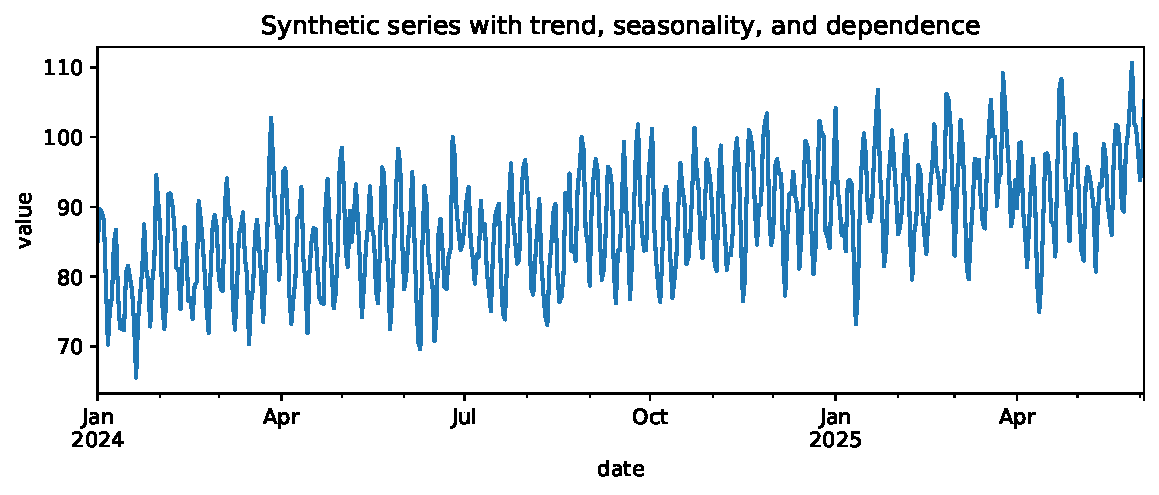
\includegraphics[keepaspectratio]{chapters/chapter-17-feature-based-machine-learning_files/figure-pdf/ch17-simulate-lagged-data-output-1.pdf}}

}

\caption{Synthetic daily time series used for feature-based
forecasting.}

\end{figure}%

\begin{Shaded}
\begin{Highlighting}[]
\KeywordTok{def}\NormalTok{ make\_lagged\_features(df, y\_col}\OperatorTok{=}\StringTok{"y"}\NormalTok{, max\_lag}\OperatorTok{=}\DecValTok{14}\NormalTok{, rolling\_windows}\OperatorTok{=}\NormalTok{(}\DecValTok{7}\NormalTok{, }\DecValTok{28}\NormalTok{), horizon}\OperatorTok{=}\DecValTok{1}\NormalTok{):}
\NormalTok{    out }\OperatorTok{=}\NormalTok{ df.copy()}
\NormalTok{    y }\OperatorTok{=}\NormalTok{ out[y\_col]}

    \CommentTok{\# Lag features available at forecast origin t.}
    \ControlFlowTok{for}\NormalTok{ lag }\KeywordTok{in} \BuiltInTok{range}\NormalTok{(}\DecValTok{1}\NormalTok{, max\_lag }\OperatorTok{+} \DecValTok{1}\NormalTok{):}
\NormalTok{        out[}\SpecialStringTok{f"lag\_}\SpecialCharTok{\{}\NormalTok{lag}\SpecialCharTok{\}}\SpecialStringTok{"}\NormalTok{] }\OperatorTok{=}\NormalTok{ y.shift(lag }\OperatorTok{{-}} \DecValTok{1}\NormalTok{)}

    \CommentTok{\# Rolling features using past and current values only.}
    \ControlFlowTok{for}\NormalTok{ w }\KeywordTok{in}\NormalTok{ rolling\_windows:}
\NormalTok{        out[}\SpecialStringTok{f"roll\_mean\_}\SpecialCharTok{\{}\NormalTok{w}\SpecialCharTok{\}}\SpecialStringTok{"}\NormalTok{] }\OperatorTok{=}\NormalTok{ y.rolling(w, min\_periods}\OperatorTok{=}\NormalTok{w).mean()}
\NormalTok{        out[}\SpecialStringTok{f"roll\_std\_}\SpecialCharTok{\{}\NormalTok{w}\SpecialCharTok{\}}\SpecialStringTok{"}\NormalTok{] }\OperatorTok{=}\NormalTok{ y.rolling(w, min\_periods}\OperatorTok{=}\NormalTok{w).std()}

    \CommentTok{\# Calendar and Fourier features known in advance.}
\NormalTok{    day\_index }\OperatorTok{=}\NormalTok{ np.arange(}\BuiltInTok{len}\NormalTok{(out))}
\NormalTok{    out[}\StringTok{"day\_of\_week"}\NormalTok{] }\OperatorTok{=}\NormalTok{ out[}\StringTok{"ds"}\NormalTok{].dt.dayofweek}
\NormalTok{    out[}\StringTok{"is\_weekend"}\NormalTok{] }\OperatorTok{=}\NormalTok{ (out[}\StringTok{"day\_of\_week"}\NormalTok{] }\OperatorTok{\textgreater{}=} \DecValTok{5}\NormalTok{).astype(}\BuiltInTok{int}\NormalTok{)}
    \ControlFlowTok{for}\NormalTok{ k }\KeywordTok{in} \BuiltInTok{range}\NormalTok{(}\DecValTok{1}\NormalTok{, }\DecValTok{4}\NormalTok{):}
\NormalTok{        out[}\SpecialStringTok{f"sin\_week\_}\SpecialCharTok{\{}\NormalTok{k}\SpecialCharTok{\}}\SpecialStringTok{"}\NormalTok{] }\OperatorTok{=}\NormalTok{ np.sin(}\DecValTok{2} \OperatorTok{*}\NormalTok{ np.pi }\OperatorTok{*}\NormalTok{ k }\OperatorTok{*}\NormalTok{ day\_index }\OperatorTok{/} \DecValTok{7}\NormalTok{)}
\NormalTok{        out[}\SpecialStringTok{f"cos\_week\_}\SpecialCharTok{\{}\NormalTok{k}\SpecialCharTok{\}}\SpecialStringTok{"}\NormalTok{] }\OperatorTok{=}\NormalTok{ np.cos(}\DecValTok{2} \OperatorTok{*}\NormalTok{ np.pi }\OperatorTok{*}\NormalTok{ k }\OperatorTok{*}\NormalTok{ day\_index }\OperatorTok{/} \DecValTok{7}\NormalTok{)}

    \CommentTok{\# Label: value h steps after the forecast origin.}
\NormalTok{    out[}\SpecialStringTok{f"target\_h}\SpecialCharTok{\{}\NormalTok{horizon}\SpecialCharTok{\}}\SpecialStringTok{"}\NormalTok{] }\OperatorTok{=}\NormalTok{ y.shift(}\OperatorTok{{-}}\NormalTok{horizon)}
\NormalTok{    out }\OperatorTok{=}\NormalTok{ out.dropna().reset\_index(drop}\OperatorTok{=}\VariableTok{True}\NormalTok{)}
    \ControlFlowTok{return}\NormalTok{ out}

\NormalTok{supervised }\OperatorTok{=}\NormalTok{ make\_lagged\_features(series, max\_lag}\OperatorTok{=}\DecValTok{14}\NormalTok{, rolling\_windows}\OperatorTok{=}\NormalTok{(}\DecValTok{7}\NormalTok{, }\DecValTok{28}\NormalTok{), horizon}\OperatorTok{=}\DecValTok{7}\NormalTok{)}
\NormalTok{feature\_cols }\OperatorTok{=}\NormalTok{ [c }\ControlFlowTok{for}\NormalTok{ c }\KeywordTok{in}\NormalTok{ supervised.columns }\ControlFlowTok{if}\NormalTok{ c.startswith((}\StringTok{"lag\_"}\NormalTok{, }\StringTok{"roll\_"}\NormalTok{, }\StringTok{"sin\_"}\NormalTok{, }\StringTok{"cos\_"}\NormalTok{))] }\OperatorTok{+}\NormalTok{ [}\StringTok{"is\_weekend"}\NormalTok{]}
\NormalTok{target\_col }\OperatorTok{=} \StringTok{"target\_h7"}

\NormalTok{supervised[[}\StringTok{"ds"}\NormalTok{, }\StringTok{"y"}\NormalTok{] }\OperatorTok{+}\NormalTok{ feature\_cols[:}\DecValTok{8}\NormalTok{] }\OperatorTok{+}\NormalTok{ [target\_col]].head()}
\end{Highlighting}
\end{Shaded}

\protect\phantomsection\label{ch17-lag-feature-function}
{\def\LTcaptype{none} % do not increment counter
\begin{longtable}[]{@{}llllllllllll@{}}
\toprule\noalign{}
& ds & y & lag\_1 & lag\_2 & lag\_3 & lag\_4 & lag\_5 & lag\_6 & lag\_7
& lag\_8 & target\_h7 \\
\midrule\noalign{}
\endhead
\bottomrule\noalign{}
\endlastfoot
0 & 2024-01-28 & 79.305896 & 79.305896 & 72.866968 & 79.418827 &
81.036452 & 87.500677 & 80.944791 & 77.436235 & 73.933338 & 76.811646 \\
1 & 2024-01-29 & 81.869961 & 81.869961 & 79.305896 & 72.866968 &
79.418827 & 81.036452 & 87.500677 & 80.944791 & 77.436235 & 91.851188 \\
2 & 2024-01-30 & 94.554564 & 94.554564 & 81.869961 & 79.305896 &
72.866968 & 79.418827 & 81.036452 & 87.500677 & 80.944791 & 91.924750 \\
3 & 2024-01-31 & 90.656623 & 90.656623 & 94.554564 & 81.869961 &
79.305896 & 72.866968 & 79.418827 & 81.036452 & 87.500677 & 90.311178 \\
4 & 2024-02-01 & 86.608821 & 86.608821 & 90.656623 & 94.554564 &
81.869961 & 79.305896 & 72.866968 & 79.418827 & 81.036452 & 87.005967 \\
\end{longtable}
}

First rows of a supervised-learning table with lag, rolling, and Fourier
features.

The row indexed by date \(t\) contains features computed from
\(Y_t,Y_{t-1},\ldots\) and a label \(Y_{t+7}\). This is a direct
seven-day-ahead forecasting table.

\section{17.9 Linear and nonlinear ML
forecasters}\label{linear-and-nonlinear-ml-forecasters}

Feature-based ML can be used with many supervised-learning algorithms.

\subsection{Linear regression}\label{linear-regression}

A linear model estimates

\[
\widehat Y_{t+h\mid t}=\beta_0+\beta^\top X_t.
\]

It is interpretable and often strong when the feature design captures
the main structure.

\subsection{Ridge and lasso}\label{ridge-and-lasso}

Ridge regression stabilizes estimates when many lag and Fourier features
are correlated:

\[
\widehat\beta_{\text{ridge}}
=\arg\min_\beta
\sum_t (Y_{t+h}-\beta_0-\beta^\top X_t)^2
+\lambda\sum_j\beta_j^2.
\]

Lasso uses an \(\ell^1\) penalty:

\[
\widehat\beta_{\text{lasso}}
=\arg\min_\beta
\sum_t (Y_{t+h}-\beta_0-\beta^\top X_t)^2
+\lambda\sum_j|\beta_j|.
\]

Ridge shrinks coefficients smoothly. Lasso can set coefficients exactly
to zero.

\subsection{Random forests}\label{random-forests}

A random forest averages many decision trees:

\[
\widehat f(x)=\frac{1}{B}\sum_{b=1}^B T_b(x).
\]

Trees can discover nonlinear threshold effects and interactions, but
they do not extrapolate trend naturally unless trend is encoded through
features.

\subsection{Gradient boosting}\label{gradient-boosting}

Gradient boosting builds an additive model of trees:

\[
\widehat f_M(x)=\sum_{m=0}^M\nu T_m(x),
\]

where each new tree approximately fits the current residuals or negative
gradient. Boosting often performs well on tabular time-series features.

\begin{tcolorbox}[enhanced jigsaw, arc=.35mm, bottomrule=.15mm, bottomtitle=1mm, breakable, colback=white, colbacktitle=quarto-callout-warning-color!10!white, colframe=quarto-callout-warning-color-frame, coltitle=black, left=2mm, leftrule=.75mm, opacityback=0, opacitybacktitle=0.6, rightrule=.15mm, title=\textcolor{quarto-callout-warning-color}{\faExclamationTriangle}\hspace{0.5em}{Tree models and extrapolation}, titlerule=0mm, toprule=.15mm, toptitle=1mm]

Tree models interpolate within feature ranges. If a future trend moves
beyond the range of the training data, a tree model may flatten unless
time, trend, or external driver features make extrapolation possible.

\end{tcolorbox}

\section{17.10 Python example: chronological split and model
comparison}\label{python-example-chronological-split-and-model-comparison}

\begin{Shaded}
\begin{Highlighting}[]
\ImportTok{from}\NormalTok{ sklearn.compose }\ImportTok{import}\NormalTok{ ColumnTransformer}
\ImportTok{from}\NormalTok{ sklearn.ensemble }\ImportTok{import}\NormalTok{ GradientBoostingRegressor, RandomForestRegressor}
\ImportTok{from}\NormalTok{ sklearn.linear\_model }\ImportTok{import}\NormalTok{ Ridge}
\ImportTok{from}\NormalTok{ sklearn.metrics }\ImportTok{import}\NormalTok{ mean\_absolute\_error, mean\_squared\_error}
\ImportTok{from}\NormalTok{ sklearn.pipeline }\ImportTok{import}\NormalTok{ Pipeline}
\ImportTok{from}\NormalTok{ sklearn.preprocessing }\ImportTok{import}\NormalTok{ OneHotEncoder, StandardScaler}

\NormalTok{feature\_cols }\OperatorTok{=}\NormalTok{ [c }\ControlFlowTok{for}\NormalTok{ c }\KeywordTok{in}\NormalTok{ supervised.columns }\ControlFlowTok{if}\NormalTok{ c.startswith((}\StringTok{"lag\_"}\NormalTok{, }\StringTok{"roll\_"}\NormalTok{, }\StringTok{"sin\_"}\NormalTok{, }\StringTok{"cos\_"}\NormalTok{))]}
\NormalTok{feature\_cols }\OperatorTok{+=}\NormalTok{ [}\StringTok{"day\_of\_week"}\NormalTok{, }\StringTok{"is\_weekend"}\NormalTok{]}
\NormalTok{target\_col }\OperatorTok{=} \StringTok{"target\_h7"}

\NormalTok{split\_date }\OperatorTok{=}\NormalTok{ supervised[}\StringTok{"ds"}\NormalTok{].quantile(}\FloatTok{0.80}\NormalTok{)}
\NormalTok{train }\OperatorTok{=}\NormalTok{ supervised[supervised[}\StringTok{"ds"}\NormalTok{] }\OperatorTok{\textless{}=}\NormalTok{ split\_date].copy()}
\NormalTok{test }\OperatorTok{=}\NormalTok{ supervised[supervised[}\StringTok{"ds"}\NormalTok{] }\OperatorTok{\textgreater{}}\NormalTok{ split\_date].copy()}

\NormalTok{numeric\_features }\OperatorTok{=}\NormalTok{ [c }\ControlFlowTok{for}\NormalTok{ c }\KeywordTok{in}\NormalTok{ feature\_cols }\ControlFlowTok{if}\NormalTok{ c }\OperatorTok{!=} \StringTok{"day\_of\_week"}\NormalTok{]}
\NormalTok{categorical\_features }\OperatorTok{=}\NormalTok{ [}\StringTok{"day\_of\_week"}\NormalTok{]}

\NormalTok{preprocess\_linear }\OperatorTok{=}\NormalTok{ ColumnTransformer(}
\NormalTok{    transformers}\OperatorTok{=}\NormalTok{[}
\NormalTok{        (}\StringTok{"num"}\NormalTok{, StandardScaler(), numeric\_features),}
\NormalTok{        (}\StringTok{"cat"}\NormalTok{, OneHotEncoder(handle\_unknown}\OperatorTok{=}\StringTok{"ignore"}\NormalTok{), categorical\_features),}
\NormalTok{    ],}
\NormalTok{    remainder}\OperatorTok{=}\StringTok{"drop"}\NormalTok{,}
\NormalTok{)}

\NormalTok{preprocess\_tree }\OperatorTok{=}\NormalTok{ ColumnTransformer(}
\NormalTok{    transformers}\OperatorTok{=}\NormalTok{[}
\NormalTok{        (}\StringTok{"num"}\NormalTok{, }\StringTok{"passthrough"}\NormalTok{, numeric\_features),}
\NormalTok{        (}\StringTok{"cat"}\NormalTok{, OneHotEncoder(handle\_unknown}\OperatorTok{=}\StringTok{"ignore"}\NormalTok{), categorical\_features),}
\NormalTok{    ],}
\NormalTok{    remainder}\OperatorTok{=}\StringTok{"drop"}\NormalTok{,}
\NormalTok{)}

\NormalTok{models }\OperatorTok{=}\NormalTok{ \{}
    \StringTok{"ridge"}\NormalTok{: Pipeline([}
\NormalTok{        (}\StringTok{"prep"}\NormalTok{, preprocess\_linear),}
\NormalTok{        (}\StringTok{"model"}\NormalTok{, Ridge(alpha}\OperatorTok{=}\FloatTok{10.0}\NormalTok{)),}
\NormalTok{    ]),}
    \StringTok{"random\_forest"}\NormalTok{: Pipeline([}
\NormalTok{        (}\StringTok{"prep"}\NormalTok{, preprocess\_tree),}
\NormalTok{        (}\StringTok{"model"}\NormalTok{, RandomForestRegressor(}
\NormalTok{            n\_estimators}\OperatorTok{=}\DecValTok{120}\NormalTok{,}
\NormalTok{            min\_samples\_leaf}\OperatorTok{=}\DecValTok{5}\NormalTok{,}
\NormalTok{            random\_state}\OperatorTok{=}\DecValTok{7339}\NormalTok{,}
\NormalTok{        )),}
\NormalTok{    ]),}
    \StringTok{"gradient\_boosting"}\NormalTok{: Pipeline([}
\NormalTok{        (}\StringTok{"prep"}\NormalTok{, preprocess\_tree),}
\NormalTok{        (}\StringTok{"model"}\NormalTok{, GradientBoostingRegressor(}
\NormalTok{            n\_estimators}\OperatorTok{=}\DecValTok{120}\NormalTok{,}
\NormalTok{            learning\_rate}\OperatorTok{=}\FloatTok{0.04}\NormalTok{,}
\NormalTok{            max\_depth}\OperatorTok{=}\DecValTok{3}\NormalTok{,}
\NormalTok{            random\_state}\OperatorTok{=}\DecValTok{7339}\NormalTok{,}
\NormalTok{        )),}
\NormalTok{    ]),}
\NormalTok{\}}

\NormalTok{results }\OperatorTok{=}\NormalTok{ []}
\NormalTok{predictions }\OperatorTok{=}\NormalTok{ pd.DataFrame(\{}\StringTok{"ds"}\NormalTok{: test[}\StringTok{"ds"}\NormalTok{], }\StringTok{"actual"}\NormalTok{: test[target\_col]\})}

\ControlFlowTok{for}\NormalTok{ name, model }\KeywordTok{in}\NormalTok{ models.items():}
\NormalTok{    model.fit(train[feature\_cols], train[target\_col])}
\NormalTok{    yhat }\OperatorTok{=}\NormalTok{ model.predict(test[feature\_cols])}
\NormalTok{    predictions[name] }\OperatorTok{=}\NormalTok{ yhat}
\NormalTok{    results.append(\{}
        \StringTok{"model"}\NormalTok{: name,}
        \StringTok{"MAE"}\NormalTok{: mean\_absolute\_error(test[target\_col], yhat),}
        \StringTok{"RMSE"}\NormalTok{: np.sqrt(mean\_squared\_error(test[target\_col], yhat)),}
\NormalTok{    \})}

\NormalTok{pd.DataFrame(results).sort\_values(}\StringTok{"MAE"}\NormalTok{)}
\end{Highlighting}
\end{Shaded}

\protect\phantomsection\label{ch17-ml-model-comparison}
{\def\LTcaptype{none} % do not increment counter
\begin{longtable}[]{@{}llll@{}}
\toprule\noalign{}
& model & MAE & RMSE \\
\midrule\noalign{}
\endhead
\bottomrule\noalign{}
\endlastfoot
0 & ridge & 3.619053 & 4.643866 \\
2 & gradient\_boosting & 4.096294 & 5.187475 \\
1 & random\_forest & 4.127917 & 5.229897 \\
\end{longtable}
}

Seven-day-ahead forecasts from feature-based machine-learning models.

\begin{Shaded}
\begin{Highlighting}[]
\NormalTok{plt.figure(figsize}\OperatorTok{=}\NormalTok{(}\DecValTok{10}\NormalTok{, }\DecValTok{4}\NormalTok{))}
\NormalTok{plt.plot(predictions[}\StringTok{"ds"}\NormalTok{], predictions[}\StringTok{"actual"}\NormalTok{], label}\OperatorTok{=}\StringTok{"actual"}\NormalTok{, linewidth}\OperatorTok{=}\DecValTok{2}\NormalTok{)}
\ControlFlowTok{for}\NormalTok{ name }\KeywordTok{in}\NormalTok{ models:}
\NormalTok{    plt.plot(predictions[}\StringTok{"ds"}\NormalTok{], predictions[name], label}\OperatorTok{=}\NormalTok{name, alpha}\OperatorTok{=}\FloatTok{0.85}\NormalTok{)}
\NormalTok{plt.xlabel(}\StringTok{"date"}\NormalTok{)}
\NormalTok{plt.ylabel(}\StringTok{"seven{-}day{-}ahead target"}\NormalTok{)}
\NormalTok{plt.title(}\StringTok{"Feature{-}based ML forecasts on chronological test period"}\NormalTok{)}
\NormalTok{plt.legend()}
\NormalTok{plt.tight\_layout()}
\NormalTok{plt.show()}
\end{Highlighting}
\end{Shaded}

\begin{figure}[H]

{\centering \pandocbounded{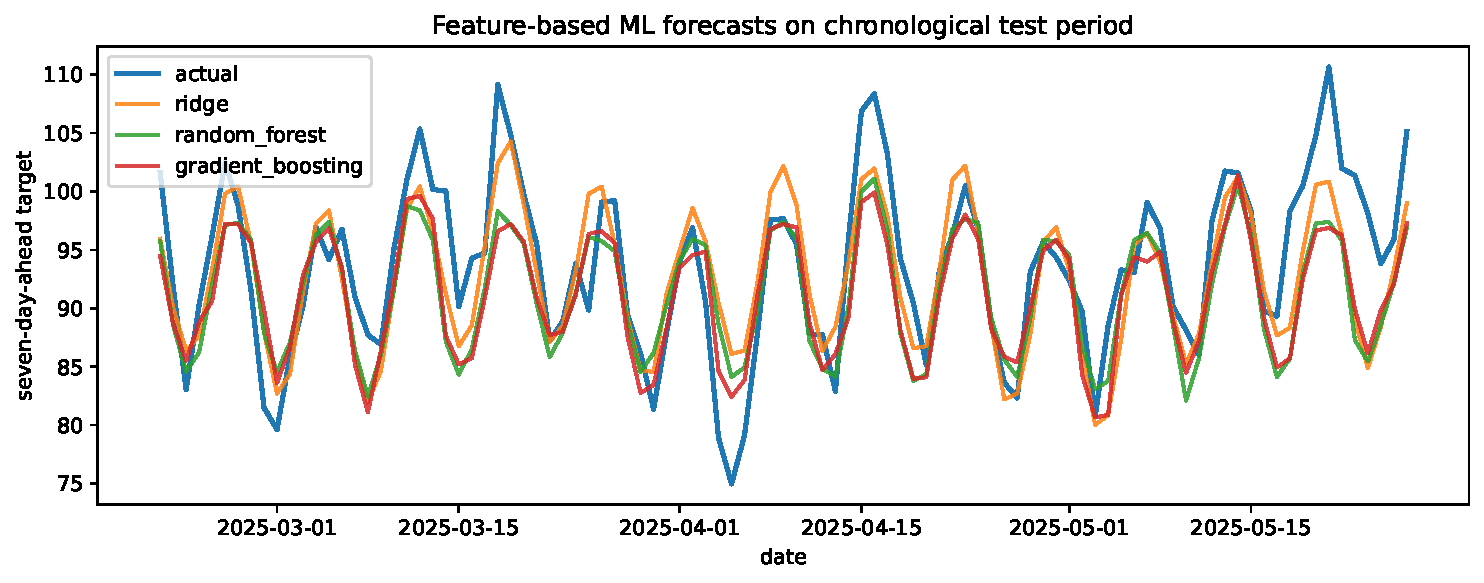
\includegraphics[keepaspectratio]{chapters/chapter-17-feature-based-machine-learning_files/figure-pdf/ch17-ml-forecast-plot-output-1.pdf}}

}

\caption{Chronological test-period forecasts from feature-based ML
models.}

\end{figure}%

\section{17.11 Recursive forecasting with a one-step
model}\label{recursive-forecasting-with-a-one-step-model}

Recursive forecasting trains a one-step model and repeatedly updates the
lag vector using predicted values. The following example illustrates the
idea with ridge regression. Recursive code is more delicate than direct
code because future feature rows do not already exist.

\begin{Shaded}
\begin{Highlighting}[]
\ImportTok{from}\NormalTok{ sklearn.pipeline }\ImportTok{import}\NormalTok{ make\_pipeline}

\NormalTok{max\_lag }\OperatorTok{=} \DecValTok{14}
\NormalTok{one\_step }\OperatorTok{=}\NormalTok{ make\_lagged\_features(series, max\_lag}\OperatorTok{=}\NormalTok{max\_lag, rolling\_windows}\OperatorTok{=}\NormalTok{(), horizon}\OperatorTok{=}\DecValTok{1}\NormalTok{)}
\NormalTok{lag\_cols }\OperatorTok{=}\NormalTok{ [}\SpecialStringTok{f"lag\_}\SpecialCharTok{\{}\NormalTok{j}\SpecialCharTok{\}}\SpecialStringTok{"} \ControlFlowTok{for}\NormalTok{ j }\KeywordTok{in} \BuiltInTok{range}\NormalTok{(}\DecValTok{1}\NormalTok{, max\_lag }\OperatorTok{+} \DecValTok{1}\NormalTok{)]}

\NormalTok{train\_end }\OperatorTok{=} \BuiltInTok{int}\NormalTok{(}\BuiltInTok{len}\NormalTok{(series) }\OperatorTok{*} \FloatTok{0.80}\NormalTok{)}
\NormalTok{train\_one }\OperatorTok{=}\NormalTok{ one\_step[one\_step.index }\OperatorTok{\textless{}}\NormalTok{ train\_end].copy()}

\NormalTok{ridge\_lag }\OperatorTok{=}\NormalTok{ make\_pipeline(StandardScaler(), Ridge(alpha}\OperatorTok{=}\FloatTok{5.0}\NormalTok{))}
\NormalTok{ridge\_lag.fit(train\_one[lag\_cols], train\_one[}\StringTok{"target\_h1"}\NormalTok{])}

\NormalTok{history }\OperatorTok{=} \BuiltInTok{list}\NormalTok{(series.loc[:train\_end }\OperatorTok{{-}} \DecValTok{1}\NormalTok{, }\StringTok{"y"}\NormalTok{].values)}
\NormalTok{H }\OperatorTok{=} \DecValTok{40}
\NormalTok{recursive\_forecast }\OperatorTok{=}\NormalTok{ []}

\ControlFlowTok{for}\NormalTok{ step }\KeywordTok{in} \BuiltInTok{range}\NormalTok{(H):}
\NormalTok{    x\_row }\OperatorTok{=}\NormalTok{ pd.DataFrame([history[}\OperatorTok{{-}}\DecValTok{1}\NormalTok{: }\OperatorTok{{-}}\NormalTok{max\_lag}\OperatorTok{{-}}\DecValTok{1}\NormalTok{: }\OperatorTok{{-}}\DecValTok{1}\NormalTok{]], columns}\OperatorTok{=}\NormalTok{lag\_cols)}
\NormalTok{    y\_next }\OperatorTok{=}\NormalTok{ ridge\_lag.predict(x\_row)[}\DecValTok{0}\NormalTok{]}
\NormalTok{    recursive\_forecast.append(y\_next)}
\NormalTok{    history.append(y\_next)}

\NormalTok{future\_dates }\OperatorTok{=}\NormalTok{ series.loc[train\_end: train\_end }\OperatorTok{+}\NormalTok{ H }\OperatorTok{{-}} \DecValTok{1}\NormalTok{, }\StringTok{"ds"}\NormalTok{].values}
\NormalTok{actual\_future }\OperatorTok{=}\NormalTok{ series.loc[train\_end: train\_end }\OperatorTok{+}\NormalTok{ H }\OperatorTok{{-}} \DecValTok{1}\NormalTok{, }\StringTok{"y"}\NormalTok{].values}

\NormalTok{plt.figure(figsize}\OperatorTok{=}\NormalTok{(}\DecValTok{9}\NormalTok{, }\FloatTok{3.5}\NormalTok{))}
\NormalTok{plt.plot(series.loc[train\_end}\OperatorTok{{-}}\DecValTok{80}\NormalTok{:train\_end}\OperatorTok{{-}}\DecValTok{1}\NormalTok{, }\StringTok{"ds"}\NormalTok{], series.loc[train\_end}\OperatorTok{{-}}\DecValTok{80}\NormalTok{:train\_end}\OperatorTok{{-}}\DecValTok{1}\NormalTok{, }\StringTok{"y"}\NormalTok{], label}\OperatorTok{=}\StringTok{"history"}\NormalTok{)}
\NormalTok{plt.plot(future\_dates, actual\_future, label}\OperatorTok{=}\StringTok{"actual future"}\NormalTok{)}
\NormalTok{plt.plot(future\_dates, recursive\_forecast, label}\OperatorTok{=}\StringTok{"recursive ridge forecast"}\NormalTok{)}
\NormalTok{plt.xlabel(}\StringTok{"date"}\NormalTok{)}
\NormalTok{plt.ylabel(}\StringTok{"value"}\NormalTok{)}
\NormalTok{plt.title(}\StringTok{"Recursive forecasting with predicted lags"}\NormalTok{)}
\NormalTok{plt.legend()}
\NormalTok{plt.tight\_layout()}
\NormalTok{plt.show()}
\end{Highlighting}
\end{Shaded}

\begin{figure}[H]

{\centering \pandocbounded{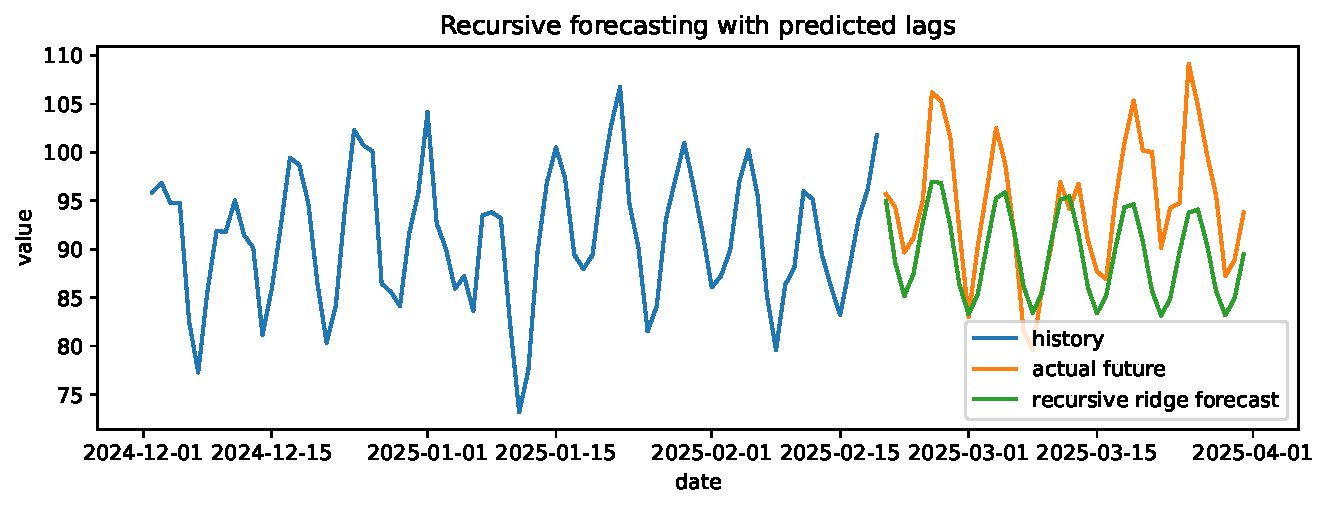
\includegraphics[keepaspectratio]{chapters/chapter-17-feature-based-machine-learning_files/figure-pdf/ch17-recursive-ridge-output-1.pdf}}

}

\caption{Recursive one-step forecasts using a lag-only ridge model.}

\end{figure}%

\begin{tcolorbox}[enhanced jigsaw, arc=.35mm, bottomrule=.15mm, bottomtitle=1mm, breakable, colback=white, colbacktitle=quarto-callout-important-color!10!white, colframe=quarto-callout-important-color-frame, coltitle=black, left=2mm, leftrule=.75mm, opacityback=0, opacitybacktitle=0.6, rightrule=.15mm, title=\textcolor{quarto-callout-important-color}{\faExclamation}\hspace{0.5em}{Recursive forecasting changes the input distribution}, titlerule=0mm, toprule=.15mm, toptitle=1mm]

During training, lag features contain observed values. During recursive
prediction, some lag features contain model predictions. This
train/predict mismatch is one reason recursive forecasts can degrade at
longer horizons.

\end{tcolorbox}

\section{17.12 Direct multi-horizon
forecasting}\label{direct-multi-horizon-forecasting}

A direct strategy trains one model per horizon. For \(H=14\), we train

\[
\widehat f_1,\widehat f_2,\ldots,\widehat f_{14}.
\]

Each model uses the same origin-time features but a different target.

\begin{Shaded}
\begin{Highlighting}[]
\NormalTok{H }\OperatorTok{=} \DecValTok{14}
\NormalTok{base }\OperatorTok{=}\NormalTok{ series.copy()}

\CommentTok{\# Origin{-}time features with no horizon{-}specific target yet.}
\NormalTok{features\_base }\OperatorTok{=}\NormalTok{ make\_lagged\_features(base, max\_lag}\OperatorTok{=}\DecValTok{14}\NormalTok{, rolling\_windows}\OperatorTok{=}\NormalTok{(}\DecValTok{7}\NormalTok{, }\DecValTok{28}\NormalTok{), horizon}\OperatorTok{=}\DecValTok{1}\NormalTok{)}
\NormalTok{feature\_cols\_direct }\OperatorTok{=}\NormalTok{ [c }\ControlFlowTok{for}\NormalTok{ c }\KeywordTok{in}\NormalTok{ features\_base.columns }\ControlFlowTok{if}\NormalTok{ c.startswith((}\StringTok{"lag\_"}\NormalTok{, }\StringTok{"roll\_"}\NormalTok{, }\StringTok{"sin\_"}\NormalTok{, }\StringTok{"cos\_"}\NormalTok{))]}
\NormalTok{feature\_cols\_direct }\OperatorTok{+=}\NormalTok{ [}\StringTok{"day\_of\_week"}\NormalTok{, }\StringTok{"is\_weekend"}\NormalTok{]}

\CommentTok{\# Add targets for all horizons.}
\ControlFlowTok{for}\NormalTok{ h }\KeywordTok{in} \BuiltInTok{range}\NormalTok{(}\DecValTok{1}\NormalTok{, H }\OperatorTok{+} \DecValTok{1}\NormalTok{):}
\NormalTok{    features\_base[}\SpecialStringTok{f"target\_h}\SpecialCharTok{\{}\NormalTok{h}\SpecialCharTok{\}}\SpecialStringTok{"}\NormalTok{] }\OperatorTok{=}\NormalTok{ series[}\StringTok{"y"}\NormalTok{].shift(}\OperatorTok{{-}}\NormalTok{h).reindex(features\_base.index).values}
\NormalTok{features\_base }\OperatorTok{=}\NormalTok{ features\_base.dropna().reset\_index(drop}\OperatorTok{=}\VariableTok{True}\NormalTok{)}

\NormalTok{origin\_date }\OperatorTok{=}\NormalTok{ features\_base[}\StringTok{"ds"}\NormalTok{].iloc[}\BuiltInTok{int}\NormalTok{(}\FloatTok{0.80} \OperatorTok{*} \BuiltInTok{len}\NormalTok{(features\_base))]}
\NormalTok{train\_direct }\OperatorTok{=}\NormalTok{ features\_base[features\_base[}\StringTok{"ds"}\NormalTok{] }\OperatorTok{\textless{}}\NormalTok{ origin\_date]}
\NormalTok{origin\_row }\OperatorTok{=}\NormalTok{ features\_base[features\_base[}\StringTok{"ds"}\NormalTok{] }\OperatorTok{==}\NormalTok{ origin\_date].iloc[[}\DecValTok{0}\NormalTok{]]}

\NormalTok{direct\_forecast }\OperatorTok{=}\NormalTok{ []}
\ControlFlowTok{for}\NormalTok{ h }\KeywordTok{in} \BuiltInTok{range}\NormalTok{(}\DecValTok{1}\NormalTok{, H }\OperatorTok{+} \DecValTok{1}\NormalTok{):}
\NormalTok{    model }\OperatorTok{=}\NormalTok{ Pipeline([}
\NormalTok{        (}\StringTok{"prep"}\NormalTok{, preprocess\_tree),}
\NormalTok{        (}\StringTok{"model"}\NormalTok{, GradientBoostingRegressor(}
\NormalTok{            n\_estimators}\OperatorTok{=}\DecValTok{80}\NormalTok{,}
\NormalTok{            learning\_rate}\OperatorTok{=}\FloatTok{0.05}\NormalTok{,}
\NormalTok{            max\_depth}\OperatorTok{=}\DecValTok{3}\NormalTok{,}
\NormalTok{            random\_state}\OperatorTok{=}\DecValTok{7339} \OperatorTok{+}\NormalTok{ h,}
\NormalTok{        )),}
\NormalTok{    ])}
\NormalTok{    model.fit(train\_direct[feature\_cols], train\_direct[}\SpecialStringTok{f"target\_h}\SpecialCharTok{\{}\NormalTok{h}\SpecialCharTok{\}}\SpecialStringTok{"}\NormalTok{])}
\NormalTok{    direct\_forecast.append(model.predict(origin\_row[feature\_cols])[}\DecValTok{0}\NormalTok{])}

\NormalTok{origin\_idx }\OperatorTok{=}\NormalTok{ series.index[series[}\StringTok{"ds"}\NormalTok{] }\OperatorTok{==}\NormalTok{ origin\_date][}\DecValTok{0}\NormalTok{]}
\NormalTok{actual\_path }\OperatorTok{=}\NormalTok{ series.loc[origin\_idx }\OperatorTok{+} \DecValTok{1}\NormalTok{: origin\_idx }\OperatorTok{+}\NormalTok{ H, }\StringTok{"y"}\NormalTok{].values}
\NormalTok{future\_dates }\OperatorTok{=}\NormalTok{ series.loc[origin\_idx }\OperatorTok{+} \DecValTok{1}\NormalTok{: origin\_idx }\OperatorTok{+}\NormalTok{ H, }\StringTok{"ds"}\NormalTok{].values}

\NormalTok{plt.figure(figsize}\OperatorTok{=}\NormalTok{(}\DecValTok{8}\NormalTok{, }\FloatTok{3.5}\NormalTok{))}
\NormalTok{plt.plot(series.loc[origin\_idx}\OperatorTok{{-}}\DecValTok{80}\NormalTok{:origin\_idx, }\StringTok{"ds"}\NormalTok{], series.loc[origin\_idx}\OperatorTok{{-}}\DecValTok{80}\NormalTok{:origin\_idx, }\StringTok{"y"}\NormalTok{], label}\OperatorTok{=}\StringTok{"history"}\NormalTok{)}
\NormalTok{plt.plot(future\_dates, actual\_path, marker}\OperatorTok{=}\StringTok{"o"}\NormalTok{, label}\OperatorTok{=}\StringTok{"actual"}\NormalTok{)}
\NormalTok{plt.plot(future\_dates, direct\_forecast, marker}\OperatorTok{=}\StringTok{"o"}\NormalTok{, label}\OperatorTok{=}\StringTok{"direct ML forecast"}\NormalTok{)}
\NormalTok{plt.xlabel(}\StringTok{"date"}\NormalTok{)}
\NormalTok{plt.ylabel(}\StringTok{"value"}\NormalTok{)}
\NormalTok{plt.title(}\StringTok{"Direct multi{-}horizon forecast"}\NormalTok{)}
\NormalTok{plt.legend()}
\NormalTok{plt.tight\_layout()}
\NormalTok{plt.show()}
\end{Highlighting}
\end{Shaded}

\begin{figure}[H]

{\centering \pandocbounded{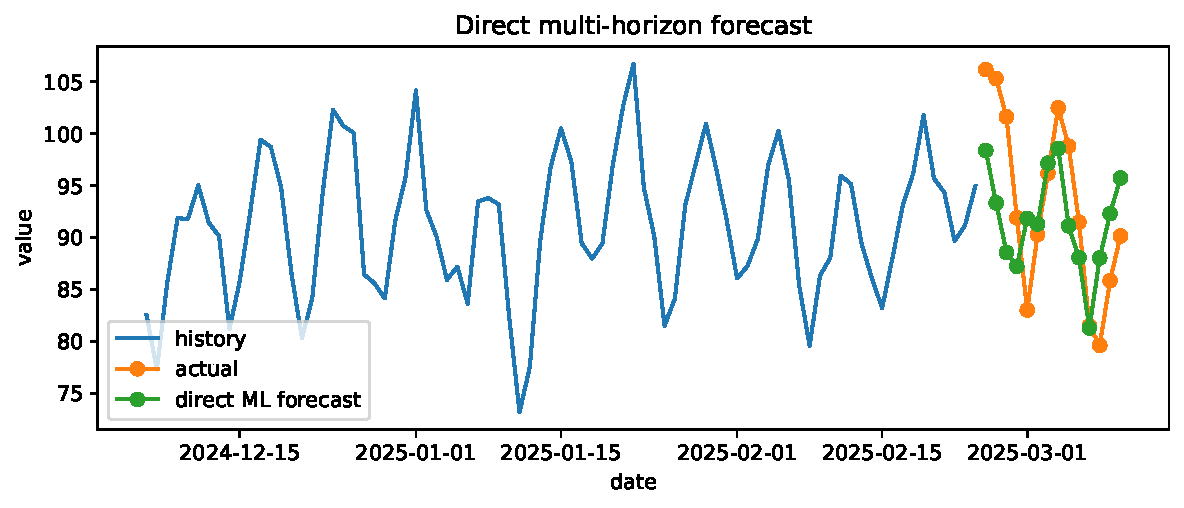
\includegraphics[keepaspectratio]{chapters/chapter-17-feature-based-machine-learning_files/figure-pdf/ch17-direct-multihorizon-output-1.pdf}}

}

\caption{Direct forecasts from separate horizon-specific models.}

\end{figure}%

\section{17.13 Rolling-origin validation for ML feature
models}\label{rolling-origin-validation-for-ml-feature-models}

The following backtest trains a model repeatedly at different forecast
origins. This is slower than a single chronological split, but it gives
a more realistic estimate of forecasting performance.

\protect\phantomsection\label{ch17-rolling-origin-ml}
\begin{Shaded}
\begin{Highlighting}[]
\KeywordTok{def}\NormalTok{ make\_features\_for\_horizon(df, horizon, max\_lag}\OperatorTok{=}\DecValTok{14}\NormalTok{):}
\NormalTok{    tab }\OperatorTok{=}\NormalTok{ make\_lagged\_features(df, max\_lag}\OperatorTok{=}\NormalTok{max\_lag, rolling\_windows}\OperatorTok{=}\NormalTok{(}\DecValTok{7}\NormalTok{, }\DecValTok{28}\NormalTok{), horizon}\OperatorTok{=}\NormalTok{horizon)}
\NormalTok{    fcols }\OperatorTok{=}\NormalTok{ [c }\ControlFlowTok{for}\NormalTok{ c }\KeywordTok{in}\NormalTok{ tab.columns }\ControlFlowTok{if}\NormalTok{ c.startswith((}\StringTok{"lag\_"}\NormalTok{, }\StringTok{"roll\_"}\NormalTok{, }\StringTok{"sin\_"}\NormalTok{, }\StringTok{"cos\_"}\NormalTok{))]}
\NormalTok{    fcols }\OperatorTok{+=}\NormalTok{ [}\StringTok{"day\_of\_week"}\NormalTok{, }\StringTok{"is\_weekend"}\NormalTok{]}
    \ControlFlowTok{return}\NormalTok{ tab, fcols, }\SpecialStringTok{f"target\_h}\SpecialCharTok{\{}\NormalTok{horizon}\SpecialCharTok{\}}\SpecialStringTok{"}

\NormalTok{origins }\OperatorTok{=}\NormalTok{ pd.date\_range(series[}\StringTok{"ds"}\NormalTok{].iloc[}\DecValTok{280}\NormalTok{], series[}\StringTok{"ds"}\NormalTok{].iloc[}\DecValTok{420}\NormalTok{], freq}\OperatorTok{=}\StringTok{"35D"}\NormalTok{)}
\NormalTok{H\_eval }\OperatorTok{=} \DecValTok{5}
\NormalTok{records }\OperatorTok{=}\NormalTok{ []}

\ControlFlowTok{for}\NormalTok{ h }\KeywordTok{in} \BuiltInTok{range}\NormalTok{(}\DecValTok{1}\NormalTok{, H\_eval }\OperatorTok{+} \DecValTok{1}\NormalTok{):}
\NormalTok{    tab, fcols, target }\OperatorTok{=}\NormalTok{ make\_features\_for\_horizon(series, horizon}\OperatorTok{=}\NormalTok{h, max\_lag}\OperatorTok{=}\DecValTok{14}\NormalTok{)}
    \ControlFlowTok{for}\NormalTok{ origin }\KeywordTok{in}\NormalTok{ origins:}
\NormalTok{        train\_h }\OperatorTok{=}\NormalTok{ tab[tab[}\StringTok{"ds"}\NormalTok{] }\OperatorTok{\textless{}=}\NormalTok{ origin]}
\NormalTok{        test\_h }\OperatorTok{=}\NormalTok{ tab[tab[}\StringTok{"ds"}\NormalTok{] }\OperatorTok{==}\NormalTok{ origin]}
        \ControlFlowTok{if} \BuiltInTok{len}\NormalTok{(train\_h) }\OperatorTok{\textless{}} \DecValTok{80} \KeywordTok{or} \BuiltInTok{len}\NormalTok{(test\_h) }\OperatorTok{==} \DecValTok{0}\NormalTok{:}
            \ControlFlowTok{continue}
\NormalTok{        model }\OperatorTok{=}\NormalTok{ Pipeline([}
\NormalTok{            (}\StringTok{"prep"}\NormalTok{, preprocess\_tree),}
\NormalTok{            (}\StringTok{"model"}\NormalTok{, GradientBoostingRegressor(}
\NormalTok{                n\_estimators}\OperatorTok{=}\DecValTok{50}\NormalTok{,}
\NormalTok{                learning\_rate}\OperatorTok{=}\FloatTok{0.05}\NormalTok{,}
\NormalTok{                max\_depth}\OperatorTok{=}\DecValTok{3}\NormalTok{,}
\NormalTok{                random\_state}\OperatorTok{=}\DecValTok{1000} \OperatorTok{+}\NormalTok{ h,}
\NormalTok{            )),}
\NormalTok{        ])}
\NormalTok{        model.fit(train\_h[fcols], train\_h[target])}
\NormalTok{        yhat }\OperatorTok{=}\NormalTok{ model.predict(test\_h[fcols])[}\DecValTok{0}\NormalTok{]}
\NormalTok{        actual }\OperatorTok{=}\NormalTok{ test\_h[target].iloc[}\DecValTok{0}\NormalTok{]}
\NormalTok{        records.append(\{}\StringTok{"origin"}\NormalTok{: origin, }\StringTok{"horizon"}\NormalTok{: h, }\StringTok{"error"}\NormalTok{: actual }\OperatorTok{{-}}\NormalTok{ yhat\})}

\NormalTok{bt }\OperatorTok{=}\NormalTok{ pd.DataFrame(records)}
\NormalTok{horizon\_summary }\OperatorTok{=}\NormalTok{ (}
\NormalTok{    bt.assign(abs\_error}\OperatorTok{=}\KeywordTok{lambda}\NormalTok{ d: d[}\StringTok{"error"}\NormalTok{].}\BuiltInTok{abs}\NormalTok{())}
\NormalTok{      .groupby(}\StringTok{"horizon"}\NormalTok{, as\_index}\OperatorTok{=}\VariableTok{False}\NormalTok{)[}\StringTok{"abs\_error"}\NormalTok{]}
\NormalTok{      .mean()}
\NormalTok{      .rename(columns}\OperatorTok{=}\NormalTok{\{}\StringTok{"abs\_error"}\NormalTok{: }\StringTok{"MAE"}\NormalTok{\})}
\NormalTok{)}

\NormalTok{plt.figure(figsize}\OperatorTok{=}\NormalTok{(}\DecValTok{7}\NormalTok{, }\FloatTok{3.5}\NormalTok{))}
\NormalTok{plt.plot(horizon\_summary[}\StringTok{"horizon"}\NormalTok{], horizon\_summary[}\StringTok{"MAE"}\NormalTok{], marker}\OperatorTok{=}\StringTok{"o"}\NormalTok{)}
\NormalTok{plt.xlabel(}\StringTok{"forecast horizon"}\NormalTok{)}
\NormalTok{plt.ylabel(}\StringTok{"MAE"}\NormalTok{)}
\NormalTok{plt.title(}\StringTok{"Rolling{-}origin MAE by horizon"}\NormalTok{)}
\NormalTok{plt.tight\_layout()}
\NormalTok{plt.show()}

\NormalTok{horizon\_summary}
\end{Highlighting}
\end{Shaded}

\begin{figure}[H]

{\centering \pandocbounded{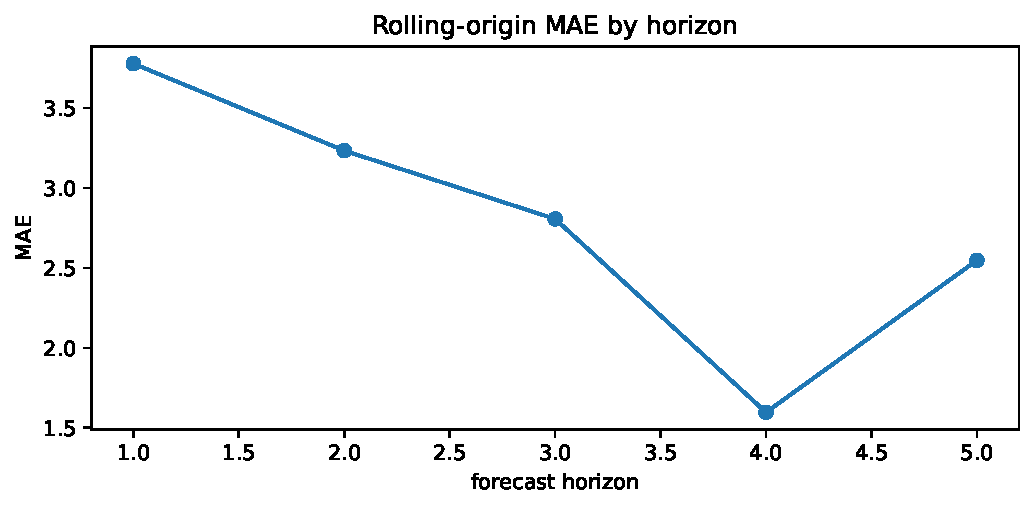
\includegraphics[keepaspectratio]{chapters/chapter-17-feature-based-machine-learning_files/figure-pdf/ch17-rolling-origin-ml-output-1.pdf}}

}

\caption{Horizon-wise MAE from rolling-origin validation.}

\end{figure}%

\protect\phantomsection\label{ch17-rolling-origin-ml-2}
{\def\LTcaptype{none} % do not increment counter
\begin{longtable}[]{@{}lll@{}}
\toprule\noalign{}
& horizon & MAE \\
\midrule\noalign{}
\endhead
\bottomrule\noalign{}
\endlastfoot
0 & 1 & 3.777906 \\
1 & 2 & 3.233628 \\
2 & 3 & 2.806294 \\
3 & 4 & 1.596699 \\
4 & 5 & 2.547511 \\
\end{longtable}
}

\section{17.14 Feature importance and
interpretation}\label{feature-importance-and-interpretation}

Feature importance can help explain a model, but it must be interpreted
carefully.

For a fitted random forest or gradient boosting model, impurity-based
importance often favors continuous variables and correlated groups.
Permutation importance is usually more meaningful: it measures the
increase in error after randomly permuting a feature.

For time-series features, correlated lag variables are common. If
\(Y_t,Y_{t-1},\ldots,Y_{t-7}\) are highly correlated, importance may be
distributed across them in unstable ways.

A more stable strategy is to group features:

\begin{itemize}
\tightlist
\item
  short lags: \(Y_t,Y_{t-1},\ldots,Y_{t-6}\);
\item
  seasonal lags: \(Y_{t-7},Y_{t-14},\ldots\);
\item
  rolling features;
\item
  Fourier/calendar features;
\item
  exogenous variables.
\end{itemize}

Then ask whether removing an entire group changes validation
performance.

\protect\phantomsection\label{ch17-permutation-importance}
\begin{Shaded}
\begin{Highlighting}[]
\ImportTok{from}\NormalTok{ sklearn.inspection }\ImportTok{import}\NormalTok{ permutation\_importance}

\NormalTok{rf }\OperatorTok{=}\NormalTok{ models[}\StringTok{"random\_forest"}\NormalTok{]}
\NormalTok{rf.fit(train[feature\_cols], train[target\_col])}
\NormalTok{perm }\OperatorTok{=}\NormalTok{ permutation\_importance(}
\NormalTok{    rf,}
\NormalTok{    test[feature\_cols],}
\NormalTok{    test[target\_col],}
\NormalTok{    n\_repeats}\OperatorTok{=}\DecValTok{5}\NormalTok{,}
\NormalTok{    random\_state}\OperatorTok{=}\DecValTok{7339}\NormalTok{,}
\NormalTok{    scoring}\OperatorTok{=}\StringTok{"neg\_mean\_absolute\_error"}\NormalTok{,}
\NormalTok{)}

\NormalTok{importance }\OperatorTok{=}\NormalTok{ (}
\NormalTok{    pd.DataFrame(\{}\StringTok{"feature"}\NormalTok{: feature\_cols, }\StringTok{"importance"}\NormalTok{: perm.importances\_mean\})}
\NormalTok{    .sort\_values(}\StringTok{"importance"}\NormalTok{, ascending}\OperatorTok{=}\VariableTok{False}\NormalTok{)}
\NormalTok{    .head(}\DecValTok{15}\NormalTok{)}
\NormalTok{)}

\NormalTok{plt.figure(figsize}\OperatorTok{=}\NormalTok{(}\DecValTok{7}\NormalTok{, }\DecValTok{4}\NormalTok{))}
\NormalTok{plt.barh(importance[}\StringTok{"feature"}\NormalTok{][::}\OperatorTok{{-}}\DecValTok{1}\NormalTok{], importance[}\StringTok{"importance"}\NormalTok{][::}\OperatorTok{{-}}\DecValTok{1}\NormalTok{])}
\NormalTok{plt.xlabel(}\StringTok{"increase in MAE after permutation"}\NormalTok{)}
\NormalTok{plt.title(}\StringTok{"Permutation importance, top features"}\NormalTok{)}
\NormalTok{plt.tight\_layout()}
\NormalTok{plt.show()}

\NormalTok{importance}
\end{Highlighting}
\end{Shaded}

\begin{figure}[H]

{\centering \pandocbounded{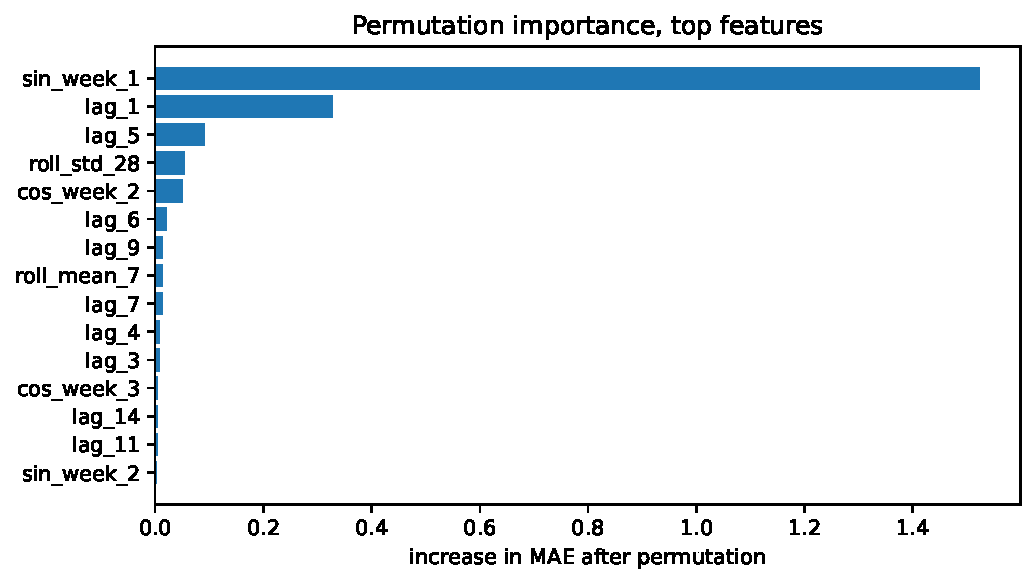
\includegraphics[keepaspectratio]{chapters/chapter-17-feature-based-machine-learning_files/figure-pdf/ch17-permutation-importance-output-1.pdf}}

}

\caption{Permutation importance on the chronological test set.}

\end{figure}%

\protect\phantomsection\label{ch17-permutation-importance-2}
{\def\LTcaptype{none} % do not increment counter
\begin{longtable}[]{@{}lll@{}}
\toprule\noalign{}
& feature & importance \\
\midrule\noalign{}
\endhead
\bottomrule\noalign{}
\endlastfoot
18 & sin\_week\_1 & 1.522503 \\
0 & lag\_1 & 0.328023 \\
4 & lag\_5 & 0.091041 \\
17 & roll\_std\_28 & 0.054667 \\
21 & cos\_week\_2 & 0.050378 \\
5 & lag\_6 & 0.020947 \\
8 & lag\_9 & 0.014119 \\
14 & roll\_mean\_7 & 0.013196 \\
6 & lag\_7 & 0.012949 \\
3 & lag\_4 & 0.008140 \\
2 & lag\_3 & 0.008133 \\
23 & cos\_week\_3 & 0.004149 \\
13 & lag\_14 & 0.003751 \\
10 & lag\_11 & 0.003486 \\
20 & sin\_week\_2 & 0.001594 \\
\end{longtable}
}

\section{17.15 Diagnostics after machine
learning}\label{diagnostics-after-machine-learning}

A flexible ML model can fit nonlinear patterns, but it can still leave
time-dependent errors. Let

\[
e_{t,h}=Y_{t+h}-\widehat Y_{t+h\mid t}.
\]

Useful diagnostics include:

\begin{enumerate}
\def\labelenumi{\arabic{enumi}.}
\tightlist
\item
  time plot of forecast errors;
\item
  ACF of forecast errors;
\item
  error versus fitted value;
\item
  error by horizon;
\item
  error by calendar group;
\item
  comparison with naive and seasonal naive baselines;
\item
  performance during regime changes or shock periods.
\end{enumerate}

If the forecast errors have strong autocorrelation, the feature set or
model may be missing temporal information. If errors vary systematically
by day of week, the seasonal features may be insufficient. If errors
grow sharply with horizon, the multi-step strategy may need revision.

\protect\phantomsection\label{ch17-error-diagnostics}
\begin{Shaded}
\begin{Highlighting}[]
\ImportTok{from}\NormalTok{ statsmodels.graphics.tsaplots }\ImportTok{import}\NormalTok{ plot\_acf}

\NormalTok{best\_name }\OperatorTok{=}\NormalTok{ pd.DataFrame(results).sort\_values(}\StringTok{"MAE"}\NormalTok{).iloc[}\DecValTok{0}\NormalTok{][}\StringTok{"model"}\NormalTok{]}
\NormalTok{errors }\OperatorTok{=}\NormalTok{ predictions[}\StringTok{"actual"}\NormalTok{] }\OperatorTok{{-}}\NormalTok{ predictions[best\_name]}

\NormalTok{fig, ax }\OperatorTok{=}\NormalTok{ plt.subplots(figsize}\OperatorTok{=}\NormalTok{(}\DecValTok{9}\NormalTok{, }\DecValTok{3}\NormalTok{))}
\NormalTok{ax.plot(predictions[}\StringTok{"ds"}\NormalTok{], errors)}
\NormalTok{ax.axhline(}\DecValTok{0}\NormalTok{, linewidth}\OperatorTok{=}\DecValTok{1}\NormalTok{)}
\NormalTok{ax.set\_xlabel(}\StringTok{"date"}\NormalTok{)}
\NormalTok{ax.set\_ylabel(}\StringTok{"forecast error"}\NormalTok{)}
\NormalTok{ax.set\_title(}\SpecialStringTok{f"Test errors for }\SpecialCharTok{\{}\NormalTok{best\_name}\SpecialCharTok{\}}\SpecialStringTok{"}\NormalTok{)}
\NormalTok{plt.tight\_layout()}
\NormalTok{plt.show()}

\NormalTok{plot\_acf(errors, lags}\OperatorTok{=}\DecValTok{30}\NormalTok{)}
\NormalTok{plt.title(}\SpecialStringTok{f"ACF of test errors for }\SpecialCharTok{\{}\NormalTok{best\_name}\SpecialCharTok{\}}\SpecialStringTok{"}\NormalTok{)}
\NormalTok{plt.show()}
\end{Highlighting}
\end{Shaded}

\begin{figure}[H]

{\centering \pandocbounded{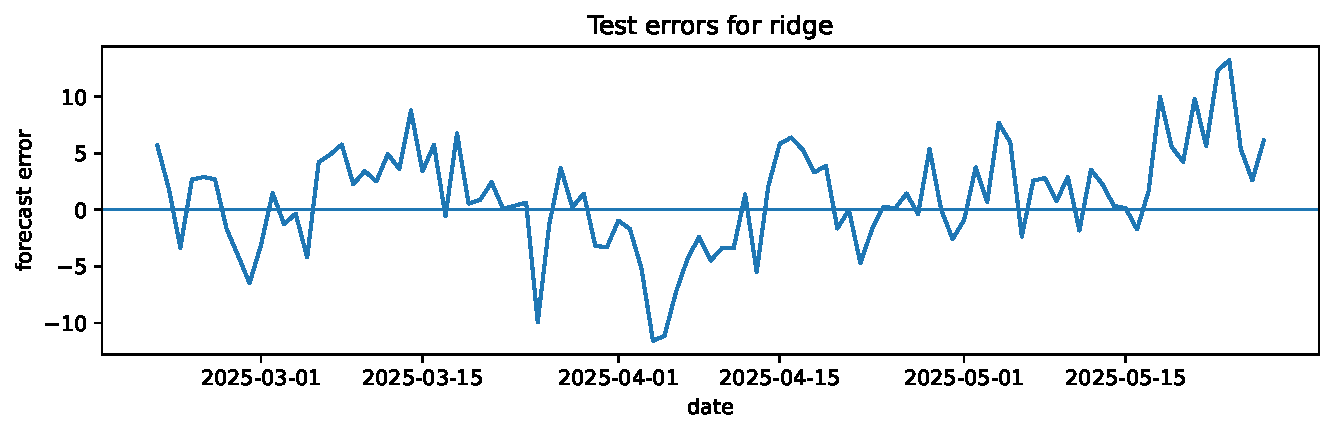
\includegraphics[keepaspectratio]{chapters/chapter-17-feature-based-machine-learning_files/figure-pdf/ch17-error-diagnostics-output-1.pdf}}

}

\caption{Test forecast errors and their sample autocorrelation.}

\end{figure}%

\pandocbounded{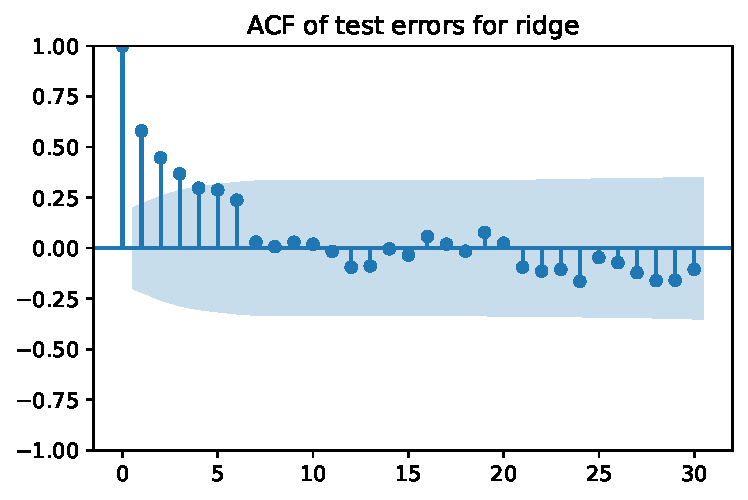
\includegraphics[keepaspectratio]{chapters/chapter-17-feature-based-machine-learning_files/figure-pdf/ch17-error-diagnostics-output-2.pdf}}

\section{17.16 Relationship with ARIMA, SARIMA, Prophet, and deep
learning}\label{relationship-with-arima-sarima-prophet-and-deep-learning}

Feature-based ML is not separate from earlier methods. It reuses many of
their ideas.

\subsection{Connection with AR models}\label{connection-with-ar-models}

An AR(\(p\)) model is a linear feature-based model with lag features:

\[
X_t=(Y_t,Y_{t-1},\ldots,Y_{t-p+1}),
\qquad
f(X_t)=\beta^\top X_t.
\]

\subsection{Connection with SARIMA}\label{connection-with-sarima}

Seasonal lags and seasonal differences inspire features such as

\[
Y_{t-s},\quad Y_{t-2s},\quad Y_t-Y_{t-s}.
\]

\subsection{Connection with Prophet-type
models}\label{connection-with-prophet-type-models}

Prophet-like models use calendar, changepoint, holiday, and Fourier
features in an additive regression structure. Feature-based ML keeps
those features but allows nonlinear functions and interactions.

\subsection{Connection with neural
networks}\label{connection-with-neural-networks}

A windowed neural network also uses features derived from a recent time
window. The difference is that neural models learn internal
representations, while feature-based ML often uses explicit handcrafted
features.

\section{17.17 AI-assisted modeling
activity}\label{ai-assisted-modeling-activity-1}

\section{AI-assisted feature engineering
prompt}\label{ai-assisted-feature-engineering-prompt}

Ask an AI assistant:

\begin{quote}
I have a daily time series with trend, weekly seasonality, possible
holidays, and autocorrelated errors. I want to forecast 1 to 14 days
ahead using feature-based machine learning. Propose lag, rolling,
Fourier, calendar, and exogenous features. For each feature, state
whether it is available at forecast origin \(t\) and identify any
leakage risk.
\end{quote}

Then verify every proposed feature manually. Delete any feature that
uses future information.

\section{AI-assisted validation
prompt}\label{ai-assisted-validation-prompt}

Ask:

\begin{quote}
Design a rolling-origin backtest for this forecast task. Include
forecast origins, horizons, metrics, baseline models, and how to
aggregate errors by horizon.
\end{quote}

Then check whether the proposed split ever trains on data after the
forecast origin. If it does, revise it.

\section{AI-assisted diagnostic
prompt}\label{ai-assisted-diagnostic-prompt}

Ask:

\begin{quote}
Given residual plots, ACF of forecast errors, and horizon-wise MAE, list
possible model failures and propose feature changes. Separate
mathematical issues from implementation issues.
\end{quote}

Use the answer as a hypothesis list, not as proof.

\section{17.18 Common mistakes}\label{common-mistakes-16}

\begin{enumerate}
\def\labelenumi{\arabic{enumi}.}
\tightlist
\item
  \textbf{Random train/test split.} This trains on future data and
  overstates performance.
\item
  \textbf{Centered rolling features.} These use future values and leak
  information.
\item
  \textbf{Using unknown future covariates.} Weather, prices, or economic
  variables may not be known at forecast time.
\item
  \textbf{Forgetting baselines.} A complicated ML model should beat
  naive and seasonal naive forecasts.
\item
  \textbf{Tuning on the test set.} Hyperparameters must be chosen using
  validation folds before final testing.
\item
  \textbf{Confusing residuals with backtest errors.} A fitted residual
  is not the same as a genuine forecast error.
\item
  \textbf{Ignoring horizon-specific behavior.} A model can be strong at
  horizon 1 and weak at horizon 14.
\item
  \textbf{Overinterpreting feature importance.} Correlated lag features
  can make individual importance unstable.
\item
  \textbf{Not matching strategy to deployment.} A direct model is not
  evaluated the same way as a recursive model.
\item
  \textbf{Assuming ML handles nonstationarity automatically.} Feature
  design and validation still matter.
\end{enumerate}

\section{17.19 Mini project: ML forecasting
pipeline}\label{mini-project-ml-forecasting-pipeline}

Choose a daily, weekly, hourly, or monthly time series. Build a
feature-based forecasting pipeline.

Your report should include:

\begin{enumerate}
\def\labelenumi{\arabic{enumi}.}
\tightlist
\item
  problem statement and forecast horizon;
\item
  time plot and EDA summary;
\item
  baseline forecasts;
\item
  feature table description;
\item
  at least two ML models;
\item
  rolling-origin validation;
\item
  horizon-wise error plot;
\item
  residual or forecast-error diagnostics;
\item
  feature-importance or feature-ablation analysis;
\item
  final recommendation and limitations.
\end{enumerate}

Suggested data sets include energy demand, transit ridership, retail
demand, weather measurements, finance, website traffic, or synthetic
data with known structure.

\section{17.20 Exercises}\label{exercises-16}

\begin{enumerate}
\def\labelenumi{\arabic{enumi}.}
\tightlist
\item
  \textbf{Lag table.} For observations \(y_1,\ldots,y_{10}\), construct
  the supervised table for \(p=3\) lags and horizon \(h=2\). Which rows
  are lost at the beginning and end?
\item
  \textbf{Leakage detection.} Decide whether each feature is valid at
  forecast origin \(t\): \(Y_t\), \(Y_{t-7}\), \(Y_{t+1}\), day of week
  at \(t+7\), weather observed at \(t+7\), scheduled holiday indicator
  at \(t+7\), centered rolling mean from \(t-3\) to \(t+3\).
\item
  \textbf{Ridge model.} Suppose \(X\in\mathbb R^{n\times p}\) and target
  vector \(y\in\mathbb R^n\). Derive the ridge estimator for a fixed
  horizon \(h\).
\item
  \textbf{Recursive versus direct.} Give a mathematical explanation for
  why recursive forecast errors can accumulate.
\item
  \textbf{Fourier features.} Write the first three sine/cosine pairs for
  weekly seasonality in daily data.
\item
  \textbf{Rolling-origin design.} Design a rolling-origin validation
  scheme for a monthly series with five years of data and a six-month
  forecast horizon.
\item
  \textbf{Baseline comparison.} Implement naive and seasonal naive
  forecasts and compare them with a random forest using lag features.
\item
  \textbf{Feature ablation.} Remove rolling features, seasonal features,
  and lag features one group at a time. Which group matters most?
\item
  \textbf{Diagnostics.} Simulate a series with a weekly seasonal
  pattern. Fit an ML model without day-of-week features. What pattern
  remains in the errors?
\item
  \textbf{AI critique.} Ask an AI assistant to design a feature set.
  Identify at least three suggestions that require leakage checks.
\end{enumerate}

\section{17.21 Chapter checklist}\label{chapter-checklist-13}

Before moving on, make sure you can:

\begin{itemize}
\tightlist
\item[$\square$]
  define a forecast origin and horizon;
\item[$\square$]
  construct a lagged supervised-learning table;
\item[$\square$]
  distinguish valid origin-time features from leakage features;
\item[$\square$]
  use calendar and Fourier features for seasonality;
\item[$\square$]
  explain recursive, direct, and multi-output forecasting;
\item[$\square$]
  implement a chronological train/test split;
\item[$\square$]
  implement rolling-origin validation;
\item[$\square$]
  compare ML models with naive and seasonal naive baselines;
\item[$\square$]
  diagnose forecast errors using plots and ACF;
\item[$\square$]
  use AI suggestions only after checking assumptions and time order.
\end{itemize}

\section{17.22 Companion Python lab}\label{companion-python-lab}

Open the companion notebook:
\href{../labs/chapter-17-feature-based-machine-learning-lab.ipynb}{\texttt{chapter-17-feature-based-machine-learning-lab.ipynb}}.

The lab asks you to build a leakage-aware ML forecasting pipeline with
lag, rolling, Fourier, and calendar features; compare linear and
tree-based models; and write a short diagnostic report.

\chapter{Probabilistic Forecasting and Uncertainty
Quantification}\label{probabilistic-forecasting-and-uncertainty-quantification}

\textbf{Part V. Forecasting at Scale and Machine Learning Methods}\\
\textbf{Chapter goal:} move from point forecasts to distributional
forecasts. We study prediction intervals, quantiles, scoring rules,
calibration, residual bootstrap methods, conformal prediction, and
uncertainty-aware forecasting workflows for classical and
machine-learning time-series models.

\section{Learning objectives}\label{learning-objectives-17}

After studying this chapter, you should be able to:

\begin{enumerate}
\def\labelenumi{\arabic{enumi}.}
\tightlist
\item
  distinguish point forecasting from probabilistic forecasting;
\item
  define forecast distributions, prediction intervals, central
  intervals, quantiles, and prediction sets;
\item
  explain why uncertainty usually grows with the forecast horizon;
\item
  derive Gaussian prediction intervals from a conditional mean and
  conditional variance;
\item
  compute empirical coverage and interval width from backtesting
  results;
\item
  use quantile loss and proper scoring rules to train and evaluate
  probabilistic forecasts;
\item
  construct residual-bootstrap prediction intervals;
\item
  construct split conformal and rolling conformal intervals for
  time-series forecasts;
\item
  diagnose miscalibrated uncertainty using coverage, interval-width, and
  PIT-style plots;
\item
  use AI assistants to critique forecast uncertainty while independently
  checking validation and assumptions.
\end{enumerate}

\section{18.1 Why point forecasts are not
enough}\label{why-point-forecasts-are-not-enough}

A point forecast gives a single number, such as

\[
\widehat Y_{t+h|t}.
\]

For many decisions, the single number is not enough. A hospital wants to
know whether tomorrow's patient volume might exceed capacity. An energy
company wants an upper-tail demand forecast. A financial-risk analyst
wants downside risk. A supply-chain planner wants a distribution of
possible demand values, not only the conditional mean.

A probabilistic forecast tries to describe the full conditional
distribution

\[
F_{t,h}(y)=\mathbb P(Y_{t+h}\le y\mid \mathcal F_t),
\]

where \(\mathcal F_t\) is the information available at forecast origin
\(t\). From this distribution we can extract:

\begin{itemize}
\tightlist
\item
  a conditional mean \(\mathbb E[Y_{t+h}\mid\mathcal F_t]\);
\item
  a conditional median;
\item
  conditional quantiles;
\item
  prediction intervals;
\item
  tail probabilities such as \(\mathbb P(Y_{t+h}>c\mid\mathcal F_t)\).
\end{itemize}

\begin{tcolorbox}[enhanced jigsaw, arc=.35mm, bottomrule=.15mm, bottomtitle=1mm, breakable, colback=white, colbacktitle=quarto-callout-note-color!10!white, colframe=quarto-callout-note-color-frame, coltitle=black, left=2mm, leftrule=.75mm, opacityback=0, opacitybacktitle=0.6, rightrule=.15mm, title=\textcolor{quarto-callout-note-color}{\faInfo}\hspace{0.5em}{Forecasting as a distributional problem}, titlerule=0mm, toprule=.15mm, toptitle=1mm]

A forecast should answer not only \textbf{what value is most likely?}
but also \textbf{how wrong could we be, and in which direction?}

\end{tcolorbox}

\section{18.2 Information sets and forecast
distributions}\label{information-sets-and-forecast-distributions}

Let \(\{Y_t\}\) be a time series and let

\[
\mathcal F_t=\sigma(Y_s, X_s: s\le t)
\]

represent the data known at time \(t\). Here \(X_s\) may include
exogenous variables, calendar features, known future schedules, or
model-generated state estimates.

A probabilistic forecast for horizon \(h\) is a conditional distribution

\[
\mathcal L(Y_{t+h}\mid \mathcal F_t),
\]

or equivalently a conditional cumulative distribution function

\[
F_{t,h}(y)=\mathbb P(Y_{t+h}\le y\mid\mathcal F_t).
\]

A point forecast is a functional of this distribution. Under squared
loss, the optimal point forecast is

\[
\widehat y_{t+h|t}^{\text{mean}}
=
\mathbb E[Y_{t+h}\mid\mathcal F_t].
\]

Under absolute loss, the optimal point forecast is a conditional median:

\[
\widehat y_{t+h|t}^{\text{median}}
\in
\{m:F_{t,h}(m)\ge 1/2,\;1-F_{t,h}(m^- )\ge 1/2\}.
\]

For asymmetric cost, the optimal point forecast is a conditional
quantile.

\section{18.3 Quantiles and prediction
intervals}\label{quantiles-and-prediction-intervals}

For \(\tau\in(0,1)\), the \(\tau\)-quantile of the conditional forecast
distribution is

\[
q_{t,h}(\tau)=F_{t,h}^{-1}(\tau)
=
\inf\{y:F_{t,h}(y)\ge \tau\}.
\]

A central \((1-\alpha)\) prediction interval is

\[
\left[q_{t,h}\left(\frac{\alpha}{2}\right),
q_{t,h}\left(1-\frac{\alpha}{2}\right)\right].
\]

For example, a 90\% central interval uses \(\alpha=0.1\):

\[
\left[q_{t,h}(0.05),q_{t,h}(0.95)\right].
\]

If the forecast distribution is conditionally Gaussian,

\[
Y_{t+h}\mid\mathcal F_t\sim N(\mu_{t,h},\sigma_{t,h}^2),
\]

then the central \((1-\alpha)\) interval is

\[
\mu_{t,h}\pm z_{1-\alpha/2}\sigma_{t,h},
\]

where \(z_{1-\alpha/2}\) is the corresponding standard normal quantile.

\section{The interval has two jobs}\label{the-interval-has-two-jobs}

A prediction interval should be \textbf{calibrated} and \textbf{sharp}.
Calibration means that the event \(Y_{t+h}\) falls inside the nominal
90\% interval about 90\% of the time. Sharpness means that, subject to
calibration, the interval should be as narrow as possible.

\section{18.4 Forecast error
decomposition}\label{forecast-error-decomposition}

Suppose a model produces a conditional mean forecast

\[
\widehat\mu_{t,h}=\widehat{\mathbb E}[Y_{t+h}\mid\mathcal F_t].
\]

The forecast error is

\[
e_{t,h}=Y_{t+h}-\widehat\mu_{t,h}.
\]

A useful conceptual decomposition is

\[
e_{t,h}
=
\underbrace{Y_{t+h}-\mathbb E[Y_{t+h}\mid\mathcal F_t]}_{\text{irreducible uncertainty}}
+
\underbrace{\mathbb E[Y_{t+h}\mid\mathcal F_t]-\widehat\mu_{t,h}}_{\text{model and estimation error}}.
\]

The first term is unavoidable even with the correct model. The second
term can be reduced through better modeling, more data, and better
validation.

In time-series forecasting, uncertainty often increases with horizon
because the model must propagate uncertainty through future unobserved
states or future forecast errors.

\section{18.5 Gaussian forecast intervals for
AR(1)}\label{gaussian-forecast-intervals-for-ar1}

Consider the stationary AR(1) model

\[
Y_t=\phi Y_{t-1}+W_t,\qquad W_t\sim WN(0,\sigma_W^2),\qquad |\phi|<1.
\]

The \(h\)-step conditional mean is

\[
\mathbb E[Y_{t+h}\mid Y_t]=\phi^hY_t.
\]

The forecast error is

\[
Y_{t+h}-\phi^hY_t
=
W_{t+h}+\phi W_{t+h-1}+\cdots+\phi^{h-1}W_{t+1}.
\]

Therefore,

\[
\operatorname{Var}(Y_{t+h}-\phi^hY_t\mid\mathcal F_t)
=
\sigma_W^2\sum_{j=0}^{h-1}\phi^{2j}
=
\sigma_W^2\frac{1-\phi^{2h}}{1-\phi^2}.
\]

Under Gaussian noise, a central \((1-\alpha)\) prediction interval is

\[
\phi^hY_t
\pm
z_{1-\alpha/2}\sigma_W
\sqrt{\frac{1-\phi^{2h}}{1-\phi^2}}.
\]

As \(h\to\infty\), the conditional mean goes to zero and the forecast
variance approaches the unconditional variance

\[
\frac{\sigma_W^2}{1-\phi^2}.
\]

\begin{tcolorbox}[enhanced jigsaw, arc=.35mm, bottomrule=.15mm, bottomtitle=1mm, breakable, colback=white, colbacktitle=quarto-callout-important-color!10!white, colframe=quarto-callout-important-color-frame, coltitle=black, left=2mm, leftrule=.75mm, opacityback=0, opacitybacktitle=0.6, rightrule=.15mm, title=\textcolor{quarto-callout-important-color}{\faExclamation}\hspace{0.5em}{Model-based intervals depend on model assumptions}, titlerule=0mm, toprule=.15mm, toptitle=1mm]

The AR(1) interval above is valid only to the extent that the AR(1),
stationarity, and Gaussian-noise assumptions are a good approximation to
the data-generating process.

\end{tcolorbox}

\section{18.6 Interactive demonstration: coverage versus interval
width}\label{interactive-demonstration-coverage-versus-interval-width}

The module below simulates a forecasting problem where the point
forecast is fixed but the interval multiplier can be changed. Students
can see the tension between empirical coverage and interval width.

Interactive Module: Calibration and Sharpness Explorer

Change the interval multiplier. Wider intervals usually increase
coverage, but they may become less useful for decision-making.

Interval multiplier:
\protect\phantomsection\label{ch18-width-value}{1.64}

True noise scale: \protect\phantomsection\label{ch18-noise-value}{1.00}

\protect\phantomsection\label{ch18-calibration-plot}

\section{18.7 Python example: model-based AR(1) forecast
intervals}\label{python-example-model-based-ar1-forecast-intervals}

\begin{Shaded}
\begin{Highlighting}[]
\ImportTok{import}\NormalTok{ numpy }\ImportTok{as}\NormalTok{ np}
\ImportTok{import}\NormalTok{ pandas }\ImportTok{as}\NormalTok{ pd}
\ImportTok{import}\NormalTok{ matplotlib.pyplot }\ImportTok{as}\NormalTok{ plt}

\NormalTok{rng }\OperatorTok{=}\NormalTok{ np.random.default\_rng(}\DecValTok{7339}\NormalTok{)}

\NormalTok{phi }\OperatorTok{=} \FloatTok{0.75}
\NormalTok{sigma\_w }\OperatorTok{=} \FloatTok{1.0}
\NormalTok{n }\OperatorTok{=} \DecValTok{220}
\NormalTok{y }\OperatorTok{=}\NormalTok{ np.zeros(n)}
\ControlFlowTok{for}\NormalTok{ t }\KeywordTok{in} \BuiltInTok{range}\NormalTok{(}\DecValTok{1}\NormalTok{, n):}
\NormalTok{    y[t] }\OperatorTok{=}\NormalTok{ phi }\OperatorTok{*}\NormalTok{ y[t}\OperatorTok{{-}}\DecValTok{1}\NormalTok{] }\OperatorTok{+}\NormalTok{ rng.normal(}\DecValTok{0}\NormalTok{, sigma\_w)}

\NormalTok{origin }\OperatorTok{=} \DecValTok{180}
\NormalTok{H }\OperatorTok{=} \DecValTok{30}
\NormalTok{last }\OperatorTok{=}\NormalTok{ y[origin]}
\NormalTok{h }\OperatorTok{=}\NormalTok{ np.arange(}\DecValTok{1}\NormalTok{, H }\OperatorTok{+} \DecValTok{1}\NormalTok{)}
\NormalTok{mean\_fcst }\OperatorTok{=}\NormalTok{ (phi }\OperatorTok{**}\NormalTok{ h) }\OperatorTok{*}\NormalTok{ last}
\NormalTok{var\_fcst }\OperatorTok{=}\NormalTok{ sigma\_w}\OperatorTok{**}\DecValTok{2} \OperatorTok{*}\NormalTok{ (}\DecValTok{1} \OperatorTok{{-}}\NormalTok{ phi }\OperatorTok{**}\NormalTok{ (}\DecValTok{2} \OperatorTok{*}\NormalTok{ h)) }\OperatorTok{/}\NormalTok{ (}\DecValTok{1} \OperatorTok{{-}}\NormalTok{ phi}\OperatorTok{**}\DecValTok{2}\NormalTok{)}
\NormalTok{se\_fcst }\OperatorTok{=}\NormalTok{ np.sqrt(var\_fcst)}
\NormalTok{z90 }\OperatorTok{=} \FloatTok{1.6448536269514722}
\NormalTok{lower }\OperatorTok{=}\NormalTok{ mean\_fcst }\OperatorTok{{-}}\NormalTok{ z90 }\OperatorTok{*}\NormalTok{ se\_fcst}
\NormalTok{upper }\OperatorTok{=}\NormalTok{ mean\_fcst }\OperatorTok{+}\NormalTok{ z90 }\OperatorTok{*}\NormalTok{ se\_fcst}

\NormalTok{future\_index }\OperatorTok{=}\NormalTok{ np.arange(origin }\OperatorTok{+} \DecValTok{1}\NormalTok{, origin }\OperatorTok{+}\NormalTok{ H }\OperatorTok{+} \DecValTok{1}\NormalTok{)}

\NormalTok{plt.figure(figsize}\OperatorTok{=}\NormalTok{(}\DecValTok{9}\NormalTok{, }\DecValTok{4}\NormalTok{))}
\NormalTok{plt.plot(np.arange(origin }\OperatorTok{{-}} \DecValTok{80}\NormalTok{, origin }\OperatorTok{+} \DecValTok{1}\NormalTok{), y[origin}\OperatorTok{{-}}\DecValTok{80}\NormalTok{:origin}\OperatorTok{+}\DecValTok{1}\NormalTok{], label}\OperatorTok{=}\StringTok{"observed"}\NormalTok{)}
\NormalTok{plt.plot(future\_index, y[origin}\OperatorTok{+}\DecValTok{1}\NormalTok{:origin}\OperatorTok{+}\NormalTok{H}\OperatorTok{+}\DecValTok{1}\NormalTok{], label}\OperatorTok{=}\StringTok{"future observed"}\NormalTok{)}
\NormalTok{plt.plot(future\_index, mean\_fcst, label}\OperatorTok{=}\StringTok{"AR(1) mean forecast"}\NormalTok{)}
\NormalTok{plt.fill\_between(future\_index, lower, upper, alpha}\OperatorTok{=}\FloatTok{0.25}\NormalTok{, label}\OperatorTok{=}\StringTok{"90}\SpecialCharTok{\% i}\StringTok{nterval"}\NormalTok{)}
\NormalTok{plt.axvline(origin, linestyle}\OperatorTok{=}\StringTok{"{-}{-}"}\NormalTok{, linewidth}\OperatorTok{=}\DecValTok{1}\NormalTok{)}
\NormalTok{plt.xlabel(}\StringTok{"time"}\NormalTok{)}
\NormalTok{plt.ylabel(}\StringTok{"value"}\NormalTok{)}
\NormalTok{plt.title(}\StringTok{"Model{-}based AR(1) prediction interval"}\NormalTok{)}
\NormalTok{plt.legend()}
\NormalTok{plt.show()}
\end{Highlighting}
\end{Shaded}

\begin{figure}[H]

{\centering \pandocbounded{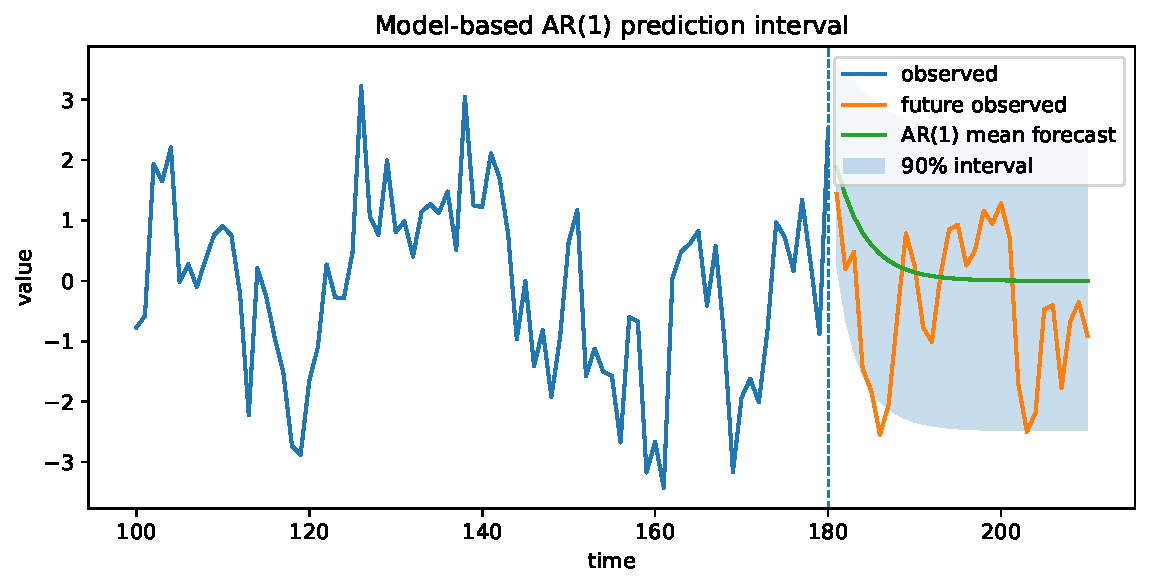
\includegraphics[keepaspectratio]{chapters/chapter-18-probabilistic-forecasting-uncertainty_files/figure-pdf/ch18-ar1-intervals-output-1.pdf}}

}

\caption{AR(1) simulation with model-based multi-step prediction
intervals.}

\end{figure}%

The formula used in the code is

\[
\widehat Y_{t+h|t}=\phi^hY_t,
\qquad
\widehat{\operatorname{Var}}(Y_{t+h}-\widehat Y_{t+h|t})
=\sigma_W^2\sum_{j=0}^{h-1}\phi^{2j}.
\]

In practice, \(\phi\) and \(\sigma_W\) are estimated. Estimation
uncertainty is usually ignored in simple textbook intervals but may
matter for small data sets.

\section{18.8 Empirical coverage and interval
width}\label{empirical-coverage-and-interval-width}

Suppose we have forecasts for origins \(t\in\mathcal T\) and horizon
\(h\). Let

\[
[L_{t,h},U_{t,h}]
\]

be a nominal \((1-\alpha)\) prediction interval. The empirical coverage
is

\[
\widehat{\operatorname{Cov}}_h
=
\frac{1}{|\mathcal T|}\sum_{t\in\mathcal T}
\mathbf 1\{L_{t,h}\le Y_{t+h}\le U_{t,h}\}.
\]

The average interval width is

\[
\widehat W_h
=
\frac{1}{|\mathcal T|}\sum_{t\in\mathcal T}(U_{t,h}-L_{t,h}).
\]

Good intervals should have empirical coverage near the nominal level and
should not be unnecessarily wide.

\begin{Shaded}
\begin{Highlighting}[]
\ImportTok{import}\NormalTok{ numpy }\ImportTok{as}\NormalTok{ np}
\ImportTok{import}\NormalTok{ pandas }\ImportTok{as}\NormalTok{ pd}
\ImportTok{import}\NormalTok{ matplotlib.pyplot }\ImportTok{as}\NormalTok{ plt}

\NormalTok{rng }\OperatorTok{=}\NormalTok{ np.random.default\_rng(}\DecValTok{18}\NormalTok{)}
\NormalTok{origins }\OperatorTok{=}\NormalTok{ np.arange(}\DecValTok{80}\NormalTok{)}
\NormalTok{horizons }\OperatorTok{=}\NormalTok{ np.arange(}\DecValTok{1}\NormalTok{, }\DecValTok{8}\NormalTok{)}
\NormalTok{rows }\OperatorTok{=}\NormalTok{ []}
\ControlFlowTok{for}\NormalTok{ h }\KeywordTok{in}\NormalTok{ horizons:}
    \ControlFlowTok{for}\NormalTok{ t }\KeywordTok{in}\NormalTok{ origins:}
\NormalTok{        true\_mean }\OperatorTok{=} \DecValTok{20} \OperatorTok{+} \FloatTok{0.1} \OperatorTok{*}\NormalTok{ t }\OperatorTok{+} \FloatTok{0.4} \OperatorTok{*}\NormalTok{ h}
\NormalTok{        true\_sd }\OperatorTok{=} \FloatTok{0.8} \OperatorTok{+} \FloatTok{0.15} \OperatorTok{*}\NormalTok{ h}
\NormalTok{        y\_true }\OperatorTok{=}\NormalTok{ true\_mean }\OperatorTok{+}\NormalTok{ rng.normal(}\DecValTok{0}\NormalTok{, true\_sd)}
        \CommentTok{\# Deliberately underestimates uncertainty at long horizons.}
\NormalTok{        model\_sd }\OperatorTok{=} \FloatTok{0.9} \OperatorTok{+} \FloatTok{0.08} \OperatorTok{*}\NormalTok{ h}
\NormalTok{        lo }\OperatorTok{=}\NormalTok{ true\_mean }\OperatorTok{{-}} \FloatTok{1.64485} \OperatorTok{*}\NormalTok{ model\_sd}
\NormalTok{        hi }\OperatorTok{=}\NormalTok{ true\_mean }\OperatorTok{+} \FloatTok{1.64485} \OperatorTok{*}\NormalTok{ model\_sd}
\NormalTok{        rows.append((t, h, y\_true, lo, hi))}

\NormalTok{bt }\OperatorTok{=}\NormalTok{ pd.DataFrame(rows, columns}\OperatorTok{=}\NormalTok{[}\StringTok{"origin"}\NormalTok{, }\StringTok{"horizon"}\NormalTok{, }\StringTok{"y"}\NormalTok{, }\StringTok{"lower"}\NormalTok{, }\StringTok{"upper"}\NormalTok{])}
\NormalTok{bt[}\StringTok{"covered"}\NormalTok{] }\OperatorTok{=}\NormalTok{ (bt[}\StringTok{"y"}\NormalTok{] }\OperatorTok{\textgreater{}=}\NormalTok{ bt[}\StringTok{"lower"}\NormalTok{]) }\OperatorTok{\&}\NormalTok{ (bt[}\StringTok{"y"}\NormalTok{] }\OperatorTok{\textless{}=}\NormalTok{ bt[}\StringTok{"upper"}\NormalTok{])}
\NormalTok{bt[}\StringTok{"width"}\NormalTok{] }\OperatorTok{=}\NormalTok{ bt[}\StringTok{"upper"}\NormalTok{] }\OperatorTok{{-}}\NormalTok{ bt[}\StringTok{"lower"}\NormalTok{]}
\NormalTok{summary }\OperatorTok{=}\NormalTok{ bt.groupby(}\StringTok{"horizon"}\NormalTok{).agg(}
\NormalTok{    coverage}\OperatorTok{=}\NormalTok{(}\StringTok{"covered"}\NormalTok{, }\StringTok{"mean"}\NormalTok{),}
\NormalTok{    avg\_width}\OperatorTok{=}\NormalTok{(}\StringTok{"width"}\NormalTok{, }\StringTok{"mean"}\NormalTok{)}
\NormalTok{).reset\_index()}

\BuiltInTok{print}\NormalTok{(summary)}

\NormalTok{plt.figure(figsize}\OperatorTok{=}\NormalTok{(}\DecValTok{7}\NormalTok{, }\DecValTok{4}\NormalTok{))}
\NormalTok{plt.plot(summary[}\StringTok{"horizon"}\NormalTok{], summary[}\StringTok{"coverage"}\NormalTok{], marker}\OperatorTok{=}\StringTok{"o"}\NormalTok{, label}\OperatorTok{=}\StringTok{"empirical coverage"}\NormalTok{)}
\NormalTok{plt.axhline(}\FloatTok{0.90}\NormalTok{, linestyle}\OperatorTok{=}\StringTok{"{-}{-}"}\NormalTok{, label}\OperatorTok{=}\StringTok{"nominal 90\%"}\NormalTok{)}
\NormalTok{plt.xlabel(}\StringTok{"forecast horizon"}\NormalTok{)}
\NormalTok{plt.ylabel(}\StringTok{"coverage"}\NormalTok{)}
\NormalTok{plt.ylim(}\FloatTok{0.4}\NormalTok{, }\FloatTok{1.0}\NormalTok{)}
\NormalTok{plt.title(}\StringTok{"Interval coverage by horizon"}\NormalTok{)}
\NormalTok{plt.legend()}
\NormalTok{plt.show()}
\end{Highlighting}
\end{Shaded}

\begin{verbatim}
   horizon  coverage  avg_width
0        1    0.9250   3.223906
1        2    0.8875   3.487082
2        3    0.8500   3.750258
3        4    0.7750   4.013434
4        5    0.8000   4.276610
5        6    0.8250   4.539786
6        7    0.7625   4.802962
\end{verbatim}

\begin{figure}[H]

{\centering \pandocbounded{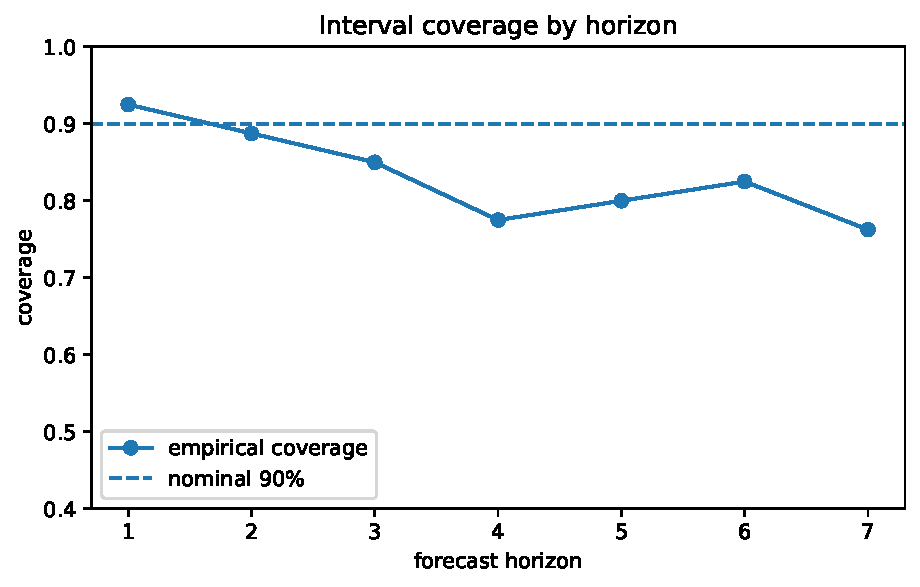
\includegraphics[keepaspectratio]{chapters/chapter-18-probabilistic-forecasting-uncertainty_files/figure-pdf/ch18-coverage-width-output-2.pdf}}

}

\caption{Coverage and width can be summarized by forecast horizon.}

\end{figure}%

\begin{tcolorbox}[enhanced jigsaw, arc=.35mm, bottomrule=.15mm, bottomtitle=1mm, breakable, colback=white, colbacktitle=quarto-callout-tip-color!10!white, colframe=quarto-callout-tip-color-frame, coltitle=black, left=2mm, leftrule=.75mm, opacityback=0, opacitybacktitle=0.6, rightrule=.15mm, title=\textcolor{quarto-callout-tip-color}{\faLightbulb}\hspace{0.5em}{Always evaluate by horizon}, titlerule=0mm, toprule=.15mm, toptitle=1mm]

A model can have acceptable average coverage across all horizons while
failing badly at longer horizons. Coverage, width, and error should be
reported by horizon whenever possible.

\end{tcolorbox}

\section{18.9 Proper scoring rules}\label{proper-scoring-rules}

A point forecast can be evaluated using MAE or RMSE. A probabilistic
forecast needs a score that rewards calibrated and sharp distributions.

A scoring rule \(S(F,y)\) assigns a loss to forecast distribution \(F\)
when the realized value is \(y\). It is \textbf{proper} if the expected
score is minimized when \(F\) equals the true conditional distribution.

\subsection{Log score}\label{log-score}

If the forecast density is \(f\), the log score is

\[
S_{\log}(f,y)=-\log f(y).
\]

It strongly penalizes assigning very low probability density to the
observed outcome.

\subsection{Pinball loss for
quantiles}\label{pinball-loss-for-quantiles}

For a quantile level \(\tau\in(0,1)\) and quantile forecast \(q\), the
pinball loss is

\[
\rho_\tau(y-q)
=(\tau-\mathbf 1\{y<q\})(y-q).
\]

Equivalently,

\[
\ell_\tau(y,q)=
\begin{cases}
\tau(y-q), & y\ge q,\\
(1-\tau)(q-y), & y<q.
\end{cases}
\]

The conditional minimizer is the \(\tau\)-quantile:

\[
q^*(x)\in\arg\min_q \mathbb E[\ell_\tau(Y,q)\mid X=x].
\]

\subsection{Winkler interval score}\label{winkler-interval-score}

For a central \((1-\alpha)\) interval \([L,U]\), the Winkler interval
score is

\[
S_\alpha(L,U;y)
=(U-L)
+\frac{2}{\alpha}(L-y)\mathbf 1\{y<L\}
+\frac{2}{\alpha}(y-U)\mathbf 1\{y>U\}.
\]

It rewards narrow intervals but penalizes misses.

\begin{Shaded}
\begin{Highlighting}[]
\ImportTok{import}\NormalTok{ numpy }\ImportTok{as}\NormalTok{ np}
\ImportTok{import}\NormalTok{ matplotlib.pyplot }\ImportTok{as}\NormalTok{ plt}

\KeywordTok{def}\NormalTok{ pinball(y, q, tau):}
\NormalTok{    u }\OperatorTok{=}\NormalTok{ y }\OperatorTok{{-}}\NormalTok{ q}
    \ControlFlowTok{return}\NormalTok{ np.maximum(tau }\OperatorTok{*}\NormalTok{ u, (tau }\OperatorTok{{-}} \DecValTok{1}\NormalTok{) }\OperatorTok{*}\NormalTok{ u)}

\NormalTok{q\_grid }\OperatorTok{=}\NormalTok{ np.linspace(}\OperatorTok{{-}}\DecValTok{3}\NormalTok{, }\DecValTok{3}\NormalTok{, }\DecValTok{300}\NormalTok{)}
\NormalTok{y\_obs }\OperatorTok{=} \FloatTok{0.0}
\NormalTok{plt.figure(figsize}\OperatorTok{=}\NormalTok{(}\DecValTok{7}\NormalTok{, }\DecValTok{4}\NormalTok{))}
\ControlFlowTok{for}\NormalTok{ tau }\KeywordTok{in}\NormalTok{ [}\FloatTok{0.1}\NormalTok{, }\FloatTok{0.5}\NormalTok{, }\FloatTok{0.9}\NormalTok{]:}
\NormalTok{    plt.plot(q\_grid, pinball(y\_obs, q\_grid, tau), label}\OperatorTok{=}\SpecialStringTok{f"tau=}\SpecialCharTok{\{}\NormalTok{tau}\SpecialCharTok{\}}\SpecialStringTok{"}\NormalTok{)}
\NormalTok{plt.xlabel(}\StringTok{"quantile forecast q"}\NormalTok{)}
\NormalTok{plt.ylabel(}\StringTok{"pinball loss"}\NormalTok{)}
\NormalTok{plt.title(}\StringTok{"Pinball loss for one observed value"}\NormalTok{)}
\NormalTok{plt.legend()}
\NormalTok{plt.show()}
\end{Highlighting}
\end{Shaded}

\begin{figure}[H]

{\centering \pandocbounded{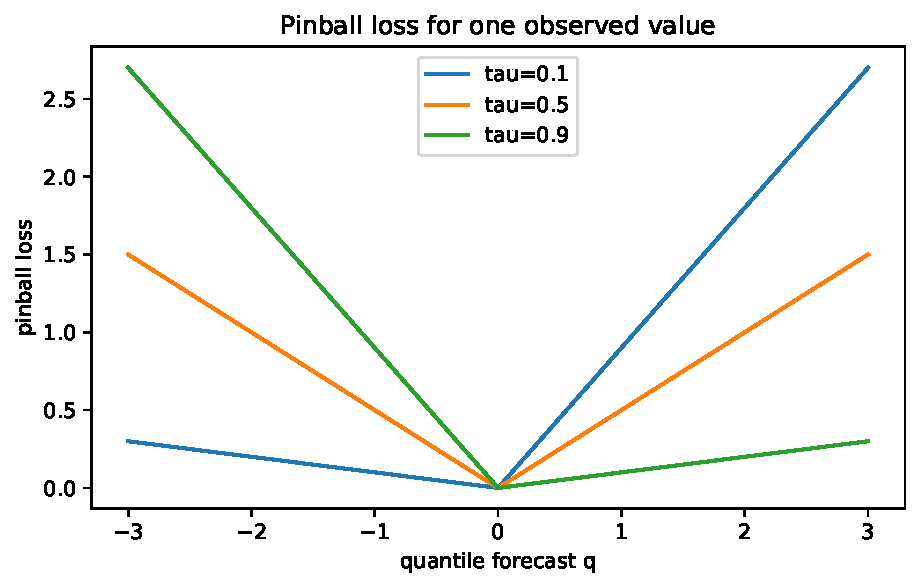
\includegraphics[keepaspectratio]{chapters/chapter-18-probabilistic-forecasting-uncertainty_files/figure-pdf/ch18-pinball-loss-output-1.pdf}}

}

\caption{Pinball loss is asymmetric and targets a conditional quantile.}

\end{figure}%

\section{18.10 Quantile regression for
forecasting}\label{quantile-regression-for-forecasting}

A machine-learning forecast can directly estimate conditional quantiles.
For horizon \(h\), choose a feature vector \(X_t\) and fit

\[
\widehat q_h(\tau,x)
\approx
F^{-1}_{Y_{t+h}\mid X_t=x}(\tau).
\]

The empirical quantile-risk problem is

\[
\widehat q_{h,\tau}
\in
\arg\min_{g\in\mathcal G}
\frac{1}{n}\sum_{t\in\mathcal T_{\text{train}}}
\ell_\tau(Y_{t+h},g(X_t)).
\]

By fitting two models, one for \(\tau=0.05\) and one for \(\tau=0.95\),
we obtain a 90\% interval.

\begin{Shaded}
\begin{Highlighting}[]
\ImportTok{import}\NormalTok{ numpy }\ImportTok{as}\NormalTok{ np}
\ImportTok{import}\NormalTok{ pandas }\ImportTok{as}\NormalTok{ pd}
\ImportTok{import}\NormalTok{ matplotlib.pyplot }\ImportTok{as}\NormalTok{ plt}
\ImportTok{from}\NormalTok{ sklearn.ensemble }\ImportTok{import}\NormalTok{ GradientBoostingRegressor}

\NormalTok{rng }\OperatorTok{=}\NormalTok{ np.random.default\_rng(}\DecValTok{7339}\NormalTok{)}
\NormalTok{n }\OperatorTok{=} \DecValTok{420}
\NormalTok{t }\OperatorTok{=}\NormalTok{ np.arange(n)}
\NormalTok{season }\OperatorTok{=}\NormalTok{ np.sin(}\DecValTok{2} \OperatorTok{*}\NormalTok{ np.pi }\OperatorTok{*}\NormalTok{ t }\OperatorTok{/} \DecValTok{24}\NormalTok{)}
\NormalTok{trend }\OperatorTok{=} \FloatTok{0.01} \OperatorTok{*}\NormalTok{ t}
\NormalTok{sigma }\OperatorTok{=} \FloatTok{0.4} \OperatorTok{+} \FloatTok{0.5} \OperatorTok{*}\NormalTok{ (season }\OperatorTok{+} \DecValTok{1}\NormalTok{)  }\CommentTok{\# larger uncertainty at seasonal peaks}
\NormalTok{y }\OperatorTok{=} \DecValTok{5} \OperatorTok{+}\NormalTok{ trend }\OperatorTok{+} \DecValTok{2} \OperatorTok{*}\NormalTok{ season }\OperatorTok{+}\NormalTok{ rng.normal(}\DecValTok{0}\NormalTok{, sigma)}

\KeywordTok{def}\NormalTok{ make\_lag\_table(y, max\_lag}\OperatorTok{=}\DecValTok{24}\NormalTok{, horizon}\OperatorTok{=}\DecValTok{1}\NormalTok{):}
\NormalTok{    rows }\OperatorTok{=}\NormalTok{ []}
\NormalTok{    targets }\OperatorTok{=}\NormalTok{ []}
\NormalTok{    times }\OperatorTok{=}\NormalTok{ []}
    \ControlFlowTok{for}\NormalTok{ i }\KeywordTok{in} \BuiltInTok{range}\NormalTok{(max\_lag, }\BuiltInTok{len}\NormalTok{(y) }\OperatorTok{{-}}\NormalTok{ horizon):}
\NormalTok{        rows.append(y[i}\OperatorTok{{-}}\NormalTok{max\_lag}\OperatorTok{+}\DecValTok{1}\NormalTok{:i}\OperatorTok{+}\DecValTok{1}\NormalTok{][::}\OperatorTok{{-}}\DecValTok{1}\NormalTok{])}
\NormalTok{        targets.append(y[i}\OperatorTok{+}\NormalTok{horizon])}
\NormalTok{        times.append(i)}
    \ControlFlowTok{return}\NormalTok{ np.asarray(rows), np.asarray(targets), np.asarray(times)}

\NormalTok{X, target, times }\OperatorTok{=}\NormalTok{ make\_lag\_table(y, max\_lag}\OperatorTok{=}\DecValTok{24}\NormalTok{, horizon}\OperatorTok{=}\DecValTok{1}\NormalTok{)}
\NormalTok{train }\OperatorTok{=}\NormalTok{ times }\OperatorTok{\textless{}} \DecValTok{300}
\NormalTok{X\_train, y\_train }\OperatorTok{=}\NormalTok{ X[train], target[train]}
\NormalTok{X\_test, y\_test, test\_times }\OperatorTok{=}\NormalTok{ X[}\OperatorTok{\textasciitilde{}}\NormalTok{train], target[}\OperatorTok{\textasciitilde{}}\NormalTok{train], times[}\OperatorTok{\textasciitilde{}}\NormalTok{train] }\OperatorTok{+} \DecValTok{1}

\NormalTok{models }\OperatorTok{=}\NormalTok{ \{\}}
\ControlFlowTok{for}\NormalTok{ tau }\KeywordTok{in}\NormalTok{ [}\FloatTok{0.05}\NormalTok{, }\FloatTok{0.5}\NormalTok{, }\FloatTok{0.95}\NormalTok{]:}
\NormalTok{    model }\OperatorTok{=}\NormalTok{ GradientBoostingRegressor(}
\NormalTok{        loss}\OperatorTok{=}\StringTok{"quantile"} \ControlFlowTok{if}\NormalTok{ tau }\OperatorTok{!=} \FloatTok{0.5} \ControlFlowTok{else} \StringTok{"squared\_error"}\NormalTok{,}
\NormalTok{        alpha}\OperatorTok{=}\NormalTok{tau }\ControlFlowTok{if}\NormalTok{ tau }\OperatorTok{!=} \FloatTok{0.5} \ControlFlowTok{else} \FloatTok{0.9}\NormalTok{,}
\NormalTok{        n\_estimators}\OperatorTok{=}\DecValTok{150}\NormalTok{,}
\NormalTok{        max\_depth}\OperatorTok{=}\DecValTok{2}\NormalTok{,}
\NormalTok{        learning\_rate}\OperatorTok{=}\FloatTok{0.05}\NormalTok{,}
\NormalTok{        random\_state}\OperatorTok{=}\DecValTok{18}
\NormalTok{    )}
\NormalTok{    model.fit(X\_train, y\_train)}
\NormalTok{    models[tau] }\OperatorTok{=}\NormalTok{ model}

\NormalTok{q05 }\OperatorTok{=}\NormalTok{ models[}\FloatTok{0.05}\NormalTok{].predict(X\_test)}
\NormalTok{q50 }\OperatorTok{=}\NormalTok{ models[}\FloatTok{0.5}\NormalTok{].predict(X\_test)}
\NormalTok{q95 }\OperatorTok{=}\NormalTok{ models[}\FloatTok{0.95}\NormalTok{].predict(X\_test)}
\NormalTok{coverage }\OperatorTok{=}\NormalTok{ np.mean((y\_test }\OperatorTok{\textgreater{}=}\NormalTok{ q05) }\OperatorTok{\&}\NormalTok{ (y\_test }\OperatorTok{\textless{}=}\NormalTok{ q95))}
\BuiltInTok{print}\NormalTok{(}\SpecialStringTok{f"Empirical 90\% interval coverage: }\SpecialCharTok{\{}\NormalTok{coverage}\SpecialCharTok{:.3f\}}\SpecialStringTok{"}\NormalTok{)}

\NormalTok{plt.figure(figsize}\OperatorTok{=}\NormalTok{(}\DecValTok{9}\NormalTok{, }\DecValTok{4}\NormalTok{))}
\NormalTok{plt.plot(t, y, linewidth}\OperatorTok{=}\DecValTok{1}\NormalTok{, label}\OperatorTok{=}\StringTok{"observed"}\NormalTok{)}
\NormalTok{plt.plot(test\_times, q50, label}\OperatorTok{=}\StringTok{"median forecast"}\NormalTok{)}
\NormalTok{plt.fill\_between(test\_times, q05, q95, alpha}\OperatorTok{=}\FloatTok{0.25}\NormalTok{, label}\OperatorTok{=}\StringTok{"estimated 90}\SpecialCharTok{\% i}\StringTok{nterval"}\NormalTok{)}
\NormalTok{plt.axvline(}\DecValTok{300}\NormalTok{, linestyle}\OperatorTok{=}\StringTok{"{-}{-}"}\NormalTok{, linewidth}\OperatorTok{=}\DecValTok{1}\NormalTok{)}
\NormalTok{plt.xlabel(}\StringTok{"time"}\NormalTok{)}
\NormalTok{plt.ylabel(}\StringTok{"value"}\NormalTok{)}
\NormalTok{plt.title(}\StringTok{"Quantile{-}regression forecast interval"}\NormalTok{)}
\NormalTok{plt.legend()}
\NormalTok{plt.show()}
\end{Highlighting}
\end{Shaded}

\begin{verbatim}
Empirical 90% interval coverage: 0.891
\end{verbatim}

\begin{figure}[H]

{\centering \pandocbounded{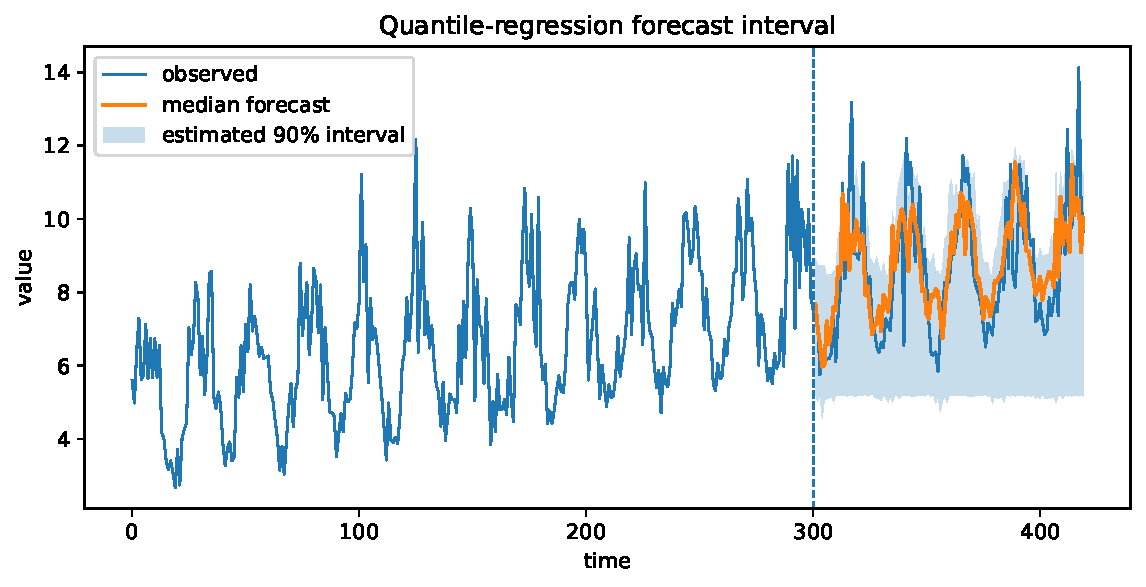
\includegraphics[keepaspectratio]{chapters/chapter-18-probabilistic-forecasting-uncertainty_files/figure-pdf/ch18-quantile-regression-output-2.pdf}}

}

\caption{Quantile regression produces asymmetric intervals when the data
are heteroskedastic.}

\end{figure}%

\section{18.11 Quantile crossing}\label{quantile-crossing}

If we fit quantile models independently, we may get crossing quantiles:

\[
\widehat q(0.95,x)<\widehat q(0.05,x),
\]

which is impossible for a valid distribution. Common fixes include:

\begin{enumerate}
\def\labelenumi{\arabic{enumi}.}
\tightlist
\item
  sorting predicted quantiles after prediction;
\item
  fitting models with monotonic constraints;
\item
  fitting a full distributional model;
\item
  using conformal calibration on top of point or quantile forecasts;
\item
  using joint neural-network quantile outputs with a non-crossing
  parameterization.
\end{enumerate}

For a classroom project, post-processing by sorting quantiles is a
reasonable first fix, but students should state that it is a repair
rather than a statistical model.

\section{18.12 Residual-bootstrap prediction
intervals}\label{residual-bootstrap-prediction-intervals}

A residual bootstrap approximates the forecast-error distribution from
past errors.

Suppose a fitted model gives one-step forecasts \(\widehat Y_{t+1|t}\).
The residuals are

\[
\widehat e_{t,1}=Y_{t+1}-\widehat Y_{t+1|t}.
\]

A simple bootstrap interval for a new one-step forecast
\(\widehat Y_{T+1|T}\) is

\[
\left[
\widehat Y_{T+1|T}+\widehat Q_{\alpha/2}(\widehat e),
\widehat Y_{T+1|T}+\widehat Q_{1-\alpha/2}(\widehat e)
\right],
\]

where \(\widehat Q_\tau(\widehat e)\) is an empirical residual quantile.

For multi-step forecasts, residuals should be grouped by horizon:

\[
\widehat e_{t,h}=Y_{t+h}-\widehat Y_{t+h|t}.
\]

Then horizon-specific intervals use horizon-specific residual quantiles.

\begin{Shaded}
\begin{Highlighting}[]
\ImportTok{import}\NormalTok{ numpy }\ImportTok{as}\NormalTok{ np}
\ImportTok{import}\NormalTok{ pandas }\ImportTok{as}\NormalTok{ pd}
\ImportTok{import}\NormalTok{ matplotlib.pyplot }\ImportTok{as}\NormalTok{ plt}
\ImportTok{from}\NormalTok{ sklearn.linear\_model }\ImportTok{import}\NormalTok{ Ridge}

\NormalTok{rng }\OperatorTok{=}\NormalTok{ np.random.default\_rng(}\DecValTok{2026}\NormalTok{)}
\NormalTok{n }\OperatorTok{=} \DecValTok{360}
\NormalTok{t }\OperatorTok{=}\NormalTok{ np.arange(n)}
\NormalTok{y }\OperatorTok{=} \DecValTok{12} \OperatorTok{+} \FloatTok{0.02}\OperatorTok{*}\NormalTok{t }\OperatorTok{+} \FloatTok{1.5}\OperatorTok{*}\NormalTok{np.sin(}\DecValTok{2}\OperatorTok{*}\NormalTok{np.pi}\OperatorTok{*}\NormalTok{t}\OperatorTok{/}\DecValTok{7}\NormalTok{) }\OperatorTok{+}\NormalTok{ rng.normal(}\DecValTok{0}\NormalTok{, }\FloatTok{0.8}\NormalTok{, size}\OperatorTok{=}\NormalTok{n)}

\NormalTok{max\_lag }\OperatorTok{=} \DecValTok{14}
\NormalTok{X, target, times }\OperatorTok{=}\NormalTok{ make\_lag\_table(y, max\_lag}\OperatorTok{=}\NormalTok{max\_lag, horizon}\OperatorTok{=}\DecValTok{1}\NormalTok{)}
\NormalTok{train }\OperatorTok{=}\NormalTok{ times }\OperatorTok{\textless{}} \DecValTok{260}
\NormalTok{cal }\OperatorTok{=}\NormalTok{ (times }\OperatorTok{\textgreater{}=} \DecValTok{260}\NormalTok{) }\OperatorTok{\&}\NormalTok{ (times }\OperatorTok{\textless{}} \DecValTok{310}\NormalTok{)}
\NormalTok{test }\OperatorTok{=}\NormalTok{ times }\OperatorTok{\textgreater{}=} \DecValTok{310}

\NormalTok{model }\OperatorTok{=}\NormalTok{ Ridge(alpha}\OperatorTok{=}\FloatTok{1.0}\NormalTok{)}
\NormalTok{model.fit(X[train], target[train])}

\NormalTok{cal\_pred }\OperatorTok{=}\NormalTok{ model.predict(X[cal])}
\NormalTok{cal\_resid }\OperatorTok{=}\NormalTok{ target[cal] }\OperatorTok{{-}}\NormalTok{ cal\_pred}
\NormalTok{lo\_resid, hi\_resid }\OperatorTok{=}\NormalTok{ np.quantile(cal\_resid, [}\FloatTok{0.05}\NormalTok{, }\FloatTok{0.95}\NormalTok{])}

\NormalTok{test\_pred }\OperatorTok{=}\NormalTok{ model.predict(X[test])}
\NormalTok{lo }\OperatorTok{=}\NormalTok{ test\_pred }\OperatorTok{+}\NormalTok{ lo\_resid}
\NormalTok{hi }\OperatorTok{=}\NormalTok{ test\_pred }\OperatorTok{+}\NormalTok{ hi\_resid}
\NormalTok{coverage }\OperatorTok{=}\NormalTok{ np.mean((target[test] }\OperatorTok{\textgreater{}=}\NormalTok{ lo) }\OperatorTok{\&}\NormalTok{ (target[test] }\OperatorTok{\textless{}=}\NormalTok{ hi))}
\BuiltInTok{print}\NormalTok{(}\SpecialStringTok{f"Bootstrap{-}style 90\% coverage on test set: }\SpecialCharTok{\{}\NormalTok{coverage}\SpecialCharTok{:.3f\}}\SpecialStringTok{"}\NormalTok{)}

\NormalTok{plt.figure(figsize}\OperatorTok{=}\NormalTok{(}\DecValTok{9}\NormalTok{, }\DecValTok{4}\NormalTok{))}
\NormalTok{test\_index }\OperatorTok{=}\NormalTok{ times[test] }\OperatorTok{+} \DecValTok{1}
\NormalTok{plt.plot(t, y, linewidth}\OperatorTok{=}\DecValTok{1}\NormalTok{, label}\OperatorTok{=}\StringTok{"observed"}\NormalTok{)}
\NormalTok{plt.plot(test\_index, test\_pred, label}\OperatorTok{=}\StringTok{"point forecast"}\NormalTok{)}
\NormalTok{plt.fill\_between(test\_index, lo, hi, alpha}\OperatorTok{=}\FloatTok{0.25}\NormalTok{, label}\OperatorTok{=}\StringTok{"residual{-}quantile interval"}\NormalTok{)}
\NormalTok{plt.axvline(}\DecValTok{310}\NormalTok{, linestyle}\OperatorTok{=}\StringTok{"{-}{-}"}\NormalTok{, linewidth}\OperatorTok{=}\DecValTok{1}\NormalTok{)}
\NormalTok{plt.xlabel(}\StringTok{"time"}\NormalTok{)}
\NormalTok{plt.ylabel(}\StringTok{"value"}\NormalTok{)}
\NormalTok{plt.title(}\StringTok{"Residual{-}bootstrap style interval"}\NormalTok{)}
\NormalTok{plt.legend()}
\NormalTok{plt.show()}
\end{Highlighting}
\end{Shaded}

\begin{verbatim}
Bootstrap-style 90% coverage on test set: 0.878
\end{verbatim}

\begin{figure}[H]

{\centering \pandocbounded{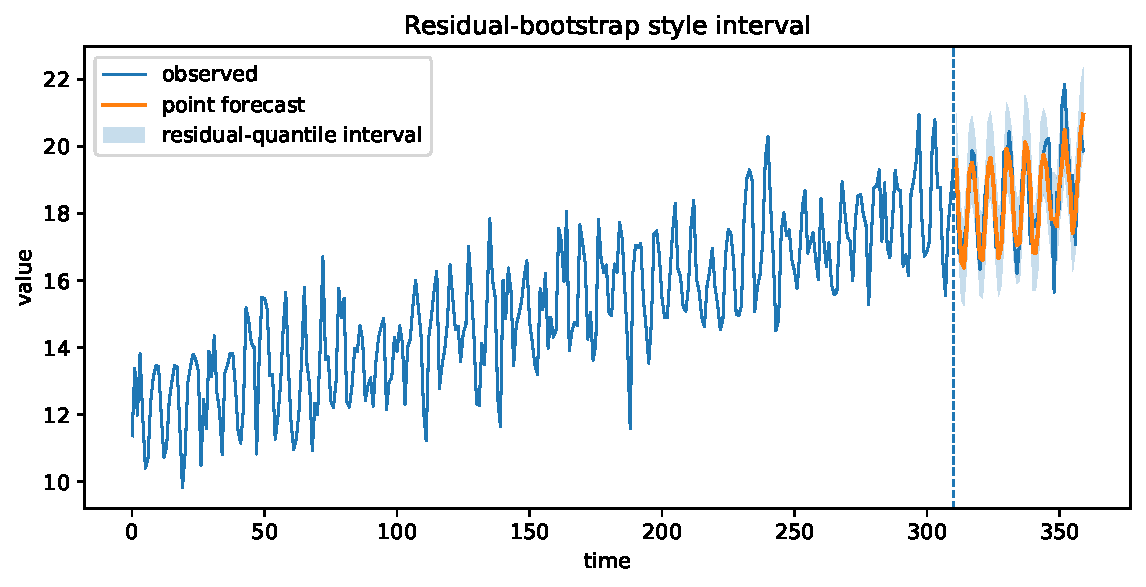
\includegraphics[keepaspectratio]{chapters/chapter-18-probabilistic-forecasting-uncertainty_files/figure-pdf/ch18-residual-bootstrap-output-2.pdf}}

}

\caption{Residual quantiles give a simple nonparametric prediction
interval.}

\end{figure}%

\begin{tcolorbox}[enhanced jigsaw, arc=.35mm, bottomrule=.15mm, bottomtitle=1mm, breakable, colback=white, colbacktitle=quarto-callout-warning-color!10!white, colframe=quarto-callout-warning-color-frame, coltitle=black, left=2mm, leftrule=.75mm, opacityback=0, opacitybacktitle=0.6, rightrule=.15mm, title=\textcolor{quarto-callout-warning-color}{\faExclamationTriangle}\hspace{0.5em}{Bootstrap residuals are not automatically valid}, titlerule=0mm, toprule=.15mm, toptitle=1mm]

Residual bootstrap intervals can fail when residuals are dependent,
heteroskedastic, seasonally structured, or drawn from a distribution
that changes over time. For time series, calibration residuals should be
chosen from a validation period that resembles future deployment.

\end{tcolorbox}

\section{18.13 Conformal prediction: distribution-free calibration
idea}\label{conformal-prediction-distribution-free-calibration-idea}

Conformal prediction constructs intervals with finite-sample coverage
guarantees under exchangeability. In time series, exchangeability is
usually not exactly true, but conformal methods are still useful when
adapted carefully through rolling calibration windows, blocked
calibration, or online updates.

For split conformal regression, fit a point model \(\widehat f\) on a
training set. On a separate calibration set, compute conformity scores

\[
s_i=|Y_i-\widehat f(X_i)|.
\]

Let \(\widehat q_{1-\alpha}\) be an appropriate empirical quantile of
the calibration scores. Then the conformal interval for a new feature
vector \(X_{\text{new}}\) is

\[
\left[
\widehat f(X_{\text{new}})-\widehat q_{1-\alpha},
\widehat f(X_{\text{new}})+\widehat q_{1-\alpha}
\right].
\]

A finite-sample conformal quantile is often chosen as

\[
\widehat q_{1-\alpha}
=\text{the }\left\lceil (n_{\text{cal}}+1)(1-\alpha)\right\rceil\text{-th smallest calibration score}.
\]

\begin{Shaded}
\begin{Highlighting}[]
\ImportTok{import}\NormalTok{ numpy }\ImportTok{as}\NormalTok{ np}
\ImportTok{import}\NormalTok{ matplotlib.pyplot }\ImportTok{as}\NormalTok{ plt}
\ImportTok{from}\NormalTok{ sklearn.ensemble }\ImportTok{import}\NormalTok{ RandomForestRegressor}

\NormalTok{rng }\OperatorTok{=}\NormalTok{ np.random.default\_rng(}\DecValTok{333}\NormalTok{)}
\NormalTok{n }\OperatorTok{=} \DecValTok{480}
\NormalTok{t }\OperatorTok{=}\NormalTok{ np.arange(n)}
\NormalTok{y }\OperatorTok{=} \DecValTok{20} \OperatorTok{+} \DecValTok{2}\OperatorTok{*}\NormalTok{np.sin(}\DecValTok{2}\OperatorTok{*}\NormalTok{np.pi}\OperatorTok{*}\NormalTok{t}\OperatorTok{/}\DecValTok{12}\NormalTok{) }\OperatorTok{+} \FloatTok{0.8}\OperatorTok{*}\NormalTok{np.sin(}\DecValTok{2}\OperatorTok{*}\NormalTok{np.pi}\OperatorTok{*}\NormalTok{t}\OperatorTok{/}\DecValTok{48}\NormalTok{)}
\NormalTok{y }\OperatorTok{=}\NormalTok{ y }\OperatorTok{+}\NormalTok{ rng.normal(}\DecValTok{0}\NormalTok{, }\FloatTok{0.9} \OperatorTok{+} \FloatTok{0.2}\OperatorTok{*}\NormalTok{np.sin(}\DecValTok{2}\OperatorTok{*}\NormalTok{np.pi}\OperatorTok{*}\NormalTok{t}\OperatorTok{/}\DecValTok{12}\NormalTok{)}\OperatorTok{**}\DecValTok{2}\NormalTok{, size}\OperatorTok{=}\NormalTok{n)}

\NormalTok{X, target, times }\OperatorTok{=}\NormalTok{ make\_lag\_table(y, max\_lag}\OperatorTok{=}\DecValTok{24}\NormalTok{, horizon}\OperatorTok{=}\DecValTok{1}\NormalTok{)}
\NormalTok{train }\OperatorTok{=}\NormalTok{ times }\OperatorTok{\textless{}} \DecValTok{280}
\NormalTok{cal }\OperatorTok{=}\NormalTok{ (times }\OperatorTok{\textgreater{}=} \DecValTok{280}\NormalTok{) }\OperatorTok{\&}\NormalTok{ (times }\OperatorTok{\textless{}} \DecValTok{380}\NormalTok{)}
\NormalTok{test }\OperatorTok{=}\NormalTok{ times }\OperatorTok{\textgreater{}=} \DecValTok{380}

\NormalTok{rf }\OperatorTok{=}\NormalTok{ RandomForestRegressor(n\_estimators}\OperatorTok{=}\DecValTok{200}\NormalTok{, min\_samples\_leaf}\OperatorTok{=}\DecValTok{4}\NormalTok{, random\_state}\OperatorTok{=}\DecValTok{18}\NormalTok{)}
\NormalTok{rf.fit(X[train], target[train])}

\NormalTok{cal\_pred }\OperatorTok{=}\NormalTok{ rf.predict(X[cal])}
\NormalTok{scores }\OperatorTok{=}\NormalTok{ np.}\BuiltInTok{abs}\NormalTok{(target[cal] }\OperatorTok{{-}}\NormalTok{ cal\_pred)}
\NormalTok{alpha }\OperatorTok{=} \FloatTok{0.10}
\NormalTok{n\_cal }\OperatorTok{=} \BuiltInTok{len}\NormalTok{(scores)}
\NormalTok{rank }\OperatorTok{=} \BuiltInTok{int}\NormalTok{(np.ceil((n\_cal }\OperatorTok{+} \DecValTok{1}\NormalTok{) }\OperatorTok{*}\NormalTok{ (}\DecValTok{1} \OperatorTok{{-}}\NormalTok{ alpha)))}
\NormalTok{rank }\OperatorTok{=} \BuiltInTok{min}\NormalTok{(rank, n\_cal)}
\NormalTok{qhat }\OperatorTok{=}\NormalTok{ np.sort(scores)[rank }\OperatorTok{{-}} \DecValTok{1}\NormalTok{]}

\NormalTok{pred }\OperatorTok{=}\NormalTok{ rf.predict(X[test])}
\NormalTok{lo }\OperatorTok{=}\NormalTok{ pred }\OperatorTok{{-}}\NormalTok{ qhat}
\NormalTok{hi }\OperatorTok{=}\NormalTok{ pred }\OperatorTok{+}\NormalTok{ qhat}
\NormalTok{covered }\OperatorTok{=}\NormalTok{ (target[test] }\OperatorTok{\textgreater{}=}\NormalTok{ lo) }\OperatorTok{\&}\NormalTok{ (target[test] }\OperatorTok{\textless{}=}\NormalTok{ hi)}
\BuiltInTok{print}\NormalTok{(}\SpecialStringTok{f"Conformal qhat: }\SpecialCharTok{\{}\NormalTok{qhat}\SpecialCharTok{:.3f\}}\SpecialStringTok{"}\NormalTok{)}
\BuiltInTok{print}\NormalTok{(}\SpecialStringTok{f"Test coverage: }\SpecialCharTok{\{}\NormalTok{covered}\SpecialCharTok{.}\NormalTok{mean()}\SpecialCharTok{:.3f\}}\SpecialStringTok{"}\NormalTok{)}

\NormalTok{plt.figure(figsize}\OperatorTok{=}\NormalTok{(}\DecValTok{9}\NormalTok{, }\DecValTok{4}\NormalTok{))}
\NormalTok{test\_index }\OperatorTok{=}\NormalTok{ times[test] }\OperatorTok{+} \DecValTok{1}
\NormalTok{plt.plot(t, y, linewidth}\OperatorTok{=}\DecValTok{1}\NormalTok{, label}\OperatorTok{=}\StringTok{"observed"}\NormalTok{)}
\NormalTok{plt.plot(test\_index, pred, label}\OperatorTok{=}\StringTok{"RF point forecast"}\NormalTok{)}
\NormalTok{plt.fill\_between(test\_index, lo, hi, alpha}\OperatorTok{=}\FloatTok{0.25}\NormalTok{, label}\OperatorTok{=}\StringTok{"split conformal interval"}\NormalTok{)}
\NormalTok{plt.axvline(}\DecValTok{380}\NormalTok{, linestyle}\OperatorTok{=}\StringTok{"{-}{-}"}\NormalTok{, linewidth}\OperatorTok{=}\DecValTok{1}\NormalTok{)}
\NormalTok{plt.xlabel(}\StringTok{"time"}\NormalTok{)}
\NormalTok{plt.ylabel(}\StringTok{"value"}\NormalTok{)}
\NormalTok{plt.title(}\StringTok{"Split conformal interval for time{-}series forecasting"}\NormalTok{)}
\NormalTok{plt.legend()}
\NormalTok{plt.show()}
\end{Highlighting}
\end{Shaded}

\begin{verbatim}
Conformal qhat: 2.061
Test coverage: 0.929
\end{verbatim}

\begin{figure}[H]

{\centering \pandocbounded{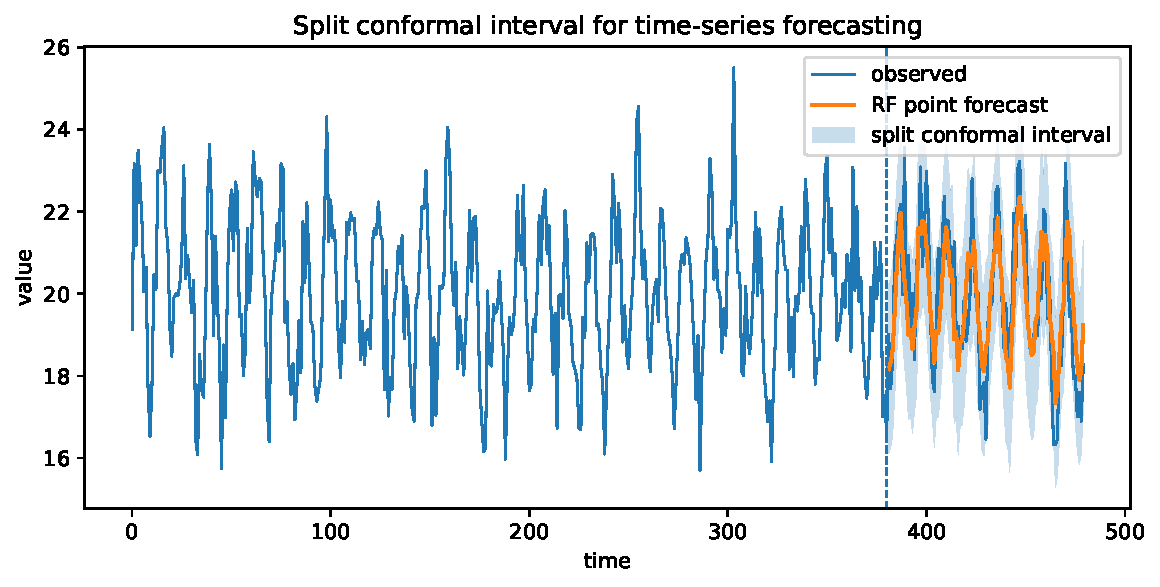
\includegraphics[keepaspectratio]{chapters/chapter-18-probabilistic-forecasting-uncertainty_files/figure-pdf/ch18-split-conformal-output-2.pdf}}

}

\caption{Split conformal intervals calibrate a point forecaster using
held-out residual scores.}

\end{figure}%

\section{18.14 Time-series conformal
prediction}\label{time-series-conformal-prediction}

Standard split conformal prediction assumes exchangeable calibration and
test points. Time series violate this because observations are ordered
and dependent. Several practical adaptations are useful:

\begin{enumerate}
\def\labelenumi{\arabic{enumi}.}
\tightlist
\item
  \textbf{Chronological split conformal.} Train on early data, calibrate
  on later data, test on the future. This respects time order but relies
  on the calibration period being representative.
\item
  \textbf{Rolling conformal.} Use a moving calibration window near the
  forecast origin.
\item
  \textbf{Horizon-specific conformal.} Calibrate a separate score
  distribution for each horizon \(h\).
\item
  \textbf{Locally weighted conformal.} Weight recent calibration errors
  more heavily.
\item
  \textbf{Normalized conformal.} Calibrate scaled scores such as
\end{enumerate}

\[
s_t=\frac{|Y_t-\widehat\mu_t|}{\widehat\sigma_t},
\]

then form

\[
[\widehat\mu_t-\widehat q\widehat\sigma_t,
\widehat\mu_t+\widehat q\widehat\sigma_t].
\]

\begin{tcolorbox}[enhanced jigsaw, arc=.35mm, bottomrule=.15mm, bottomtitle=1mm, breakable, colback=white, colbacktitle=quarto-callout-note-color!10!white, colframe=quarto-callout-note-color-frame, coltitle=black, left=2mm, leftrule=.75mm, opacityback=0, opacitybacktitle=0.6, rightrule=.15mm, title=\textcolor{quarto-callout-note-color}{\faInfo}\hspace{0.5em}{Practical rule}, titlerule=0mm, toprule=.15mm, toptitle=1mm]

For this course, use chronological or rolling calibration and report
empirical coverage on a later test period. Do not randomly shuffle
time-series residuals unless the task explicitly justifies
exchangeability.

\end{tcolorbox}

\section{18.15 Prediction intervals versus confidence
intervals}\label{prediction-intervals-versus-confidence-intervals}

A confidence interval describes uncertainty about a fixed unknown
parameter, such as a mean \(\mu\) or regression coefficient \(\beta_j\).
A prediction interval describes uncertainty about a future random
observation.

For example, in a simple Gaussian model

\[
Y_i\sim N(\mu,\sigma^2),
\]

a confidence interval for \(\mu\) shrinks roughly at rate \(1/\sqrt n\).
But a prediction interval for a future observation \(Y_{n+1}\) does not
shrink to zero width, because the new observation still has noise
variance \(\sigma^2\).

In forecasting, confusing these two intervals leads to severe
underestimation of uncertainty.

\section{18.16 Probabilistic forecasting with
simulation}\label{probabilistic-forecasting-with-simulation}

Some models do not give an easy closed-form forecast distribution.
Simulation is often the simplest method.

For a fitted model, generate future paths

\[
Y_{T+1}^{(b)},\ldots,Y_{T+H}^{(b)},\qquad b=1,\ldots,B.
\]

Then estimate quantiles at each horizon:

\[
\widehat q_h(\tau)=\operatorname{Quantile}_\tau\{Y_{T+h}^{(1)},\ldots,Y_{T+h}^{(B)}\}.
\]

Simulation is especially useful for:

\begin{itemize}
\tightlist
\item
  nonlinear state-space models;
\item
  models with non-Gaussian errors;
\item
  models with constraints, such as nonnegative demand;
\item
  hierarchical forecasts;
\item
  neural-network ensembles;
\item
  scenario analysis.
\end{itemize}

\begin{Shaded}
\begin{Highlighting}[]
\ImportTok{import}\NormalTok{ numpy }\ImportTok{as}\NormalTok{ np}
\ImportTok{import}\NormalTok{ matplotlib.pyplot }\ImportTok{as}\NormalTok{ plt}

\NormalTok{rng }\OperatorTok{=}\NormalTok{ np.random.default\_rng(}\DecValTok{91}\NormalTok{)}
\NormalTok{H }\OperatorTok{=} \DecValTok{40}
\NormalTok{B }\OperatorTok{=} \DecValTok{500}
\NormalTok{last\_y }\OperatorTok{=} \FloatTok{15.0}
\NormalTok{phi }\OperatorTok{=} \FloatTok{0.82}
\NormalTok{level }\OperatorTok{=} \FloatTok{12.0}
\NormalTok{sigma }\OperatorTok{=} \FloatTok{0.7}
\NormalTok{paths }\OperatorTok{=}\NormalTok{ np.zeros((B, H))}
\ControlFlowTok{for}\NormalTok{ b }\KeywordTok{in} \BuiltInTok{range}\NormalTok{(B):}
\NormalTok{    y\_prev }\OperatorTok{=}\NormalTok{ last\_y}
    \ControlFlowTok{for}\NormalTok{ h }\KeywordTok{in} \BuiltInTok{range}\NormalTok{(H):}
\NormalTok{        y\_new }\OperatorTok{=}\NormalTok{ level }\OperatorTok{+}\NormalTok{ phi }\OperatorTok{*}\NormalTok{ (y\_prev }\OperatorTok{{-}}\NormalTok{ level) }\OperatorTok{+}\NormalTok{ rng.normal(}\DecValTok{0}\NormalTok{, sigma)}
\NormalTok{        paths[b, h] }\OperatorTok{=}\NormalTok{ y\_new}
\NormalTok{        y\_prev }\OperatorTok{=}\NormalTok{ y\_new}

\NormalTok{median }\OperatorTok{=}\NormalTok{ np.quantile(paths, }\FloatTok{0.5}\NormalTok{, axis}\OperatorTok{=}\DecValTok{0}\NormalTok{)}
\NormalTok{lo }\OperatorTok{=}\NormalTok{ np.quantile(paths, }\FloatTok{0.05}\NormalTok{, axis}\OperatorTok{=}\DecValTok{0}\NormalTok{)}
\NormalTok{hi }\OperatorTok{=}\NormalTok{ np.quantile(paths, }\FloatTok{0.95}\NormalTok{, axis}\OperatorTok{=}\DecValTok{0}\NormalTok{)}

\NormalTok{plt.figure(figsize}\OperatorTok{=}\NormalTok{(}\DecValTok{9}\NormalTok{, }\DecValTok{4}\NormalTok{))}
\ControlFlowTok{for}\NormalTok{ b }\KeywordTok{in} \BuiltInTok{range}\NormalTok{(}\DecValTok{30}\NormalTok{):}
\NormalTok{    plt.plot(np.arange(}\DecValTok{1}\NormalTok{, H}\OperatorTok{+}\DecValTok{1}\NormalTok{), paths[b], alpha}\OperatorTok{=}\FloatTok{0.2}\NormalTok{, linewidth}\OperatorTok{=}\FloatTok{0.8}\NormalTok{)}
\NormalTok{plt.plot(np.arange(}\DecValTok{1}\NormalTok{, H}\OperatorTok{+}\DecValTok{1}\NormalTok{), median, linewidth}\OperatorTok{=}\FloatTok{2.5}\NormalTok{, label}\OperatorTok{=}\StringTok{"median"}\NormalTok{)}
\NormalTok{plt.fill\_between(np.arange(}\DecValTok{1}\NormalTok{, H}\OperatorTok{+}\DecValTok{1}\NormalTok{), lo, hi, alpha}\OperatorTok{=}\FloatTok{0.25}\NormalTok{, label}\OperatorTok{=}\StringTok{"90}\SpecialCharTok{\% s}\StringTok{imulation interval"}\NormalTok{)}
\NormalTok{plt.xlabel(}\StringTok{"horizon"}\NormalTok{)}
\NormalTok{plt.ylabel(}\StringTok{"future value"}\NormalTok{)}
\NormalTok{plt.title(}\StringTok{"Simulated future paths"}\NormalTok{)}
\NormalTok{plt.legend()}
\NormalTok{plt.show()}
\end{Highlighting}
\end{Shaded}

\begin{figure}[H]

{\centering \pandocbounded{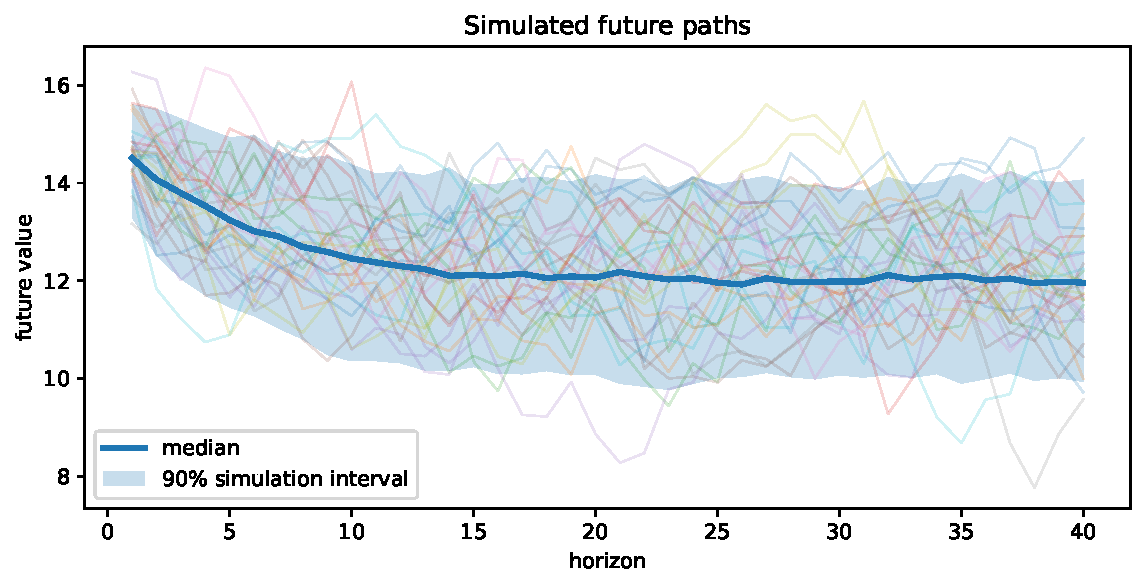
\includegraphics[keepaspectratio]{chapters/chapter-18-probabilistic-forecasting-uncertainty_files/figure-pdf/ch18-simulation-forecast-paths-output-1.pdf}}

}

\caption{Simulated forecast paths give an empirical forecast
distribution.}

\end{figure}%

\section{18.17 Bayesian predictive
distributions}\label{bayesian-predictive-distributions}

In Bayesian forecasting, parameters are treated as random variables. If
\(\theta\) denotes model parameters, then the posterior predictive
distribution is

\[
p(y_{T+h}\mid y_{1:T})
=
\int p(y_{T+h}\mid y_{1:T},\theta)p(\theta\mid y_{1:T})\,d\theta.
\]

This integral includes two kinds of uncertainty:

\begin{enumerate}
\def\labelenumi{\arabic{enumi}.}
\tightlist
\item
  \textbf{observation uncertainty}, from
  \(p(y_{T+h}\mid y_{1:T},\theta)\);
\item
  \textbf{parameter uncertainty}, from \(p(\theta\mid y_{1:T})\).
\end{enumerate}

In many classical plug-in intervals, we estimate \(\theta\) once and
ignore parameter uncertainty:

\[
p(y_{T+h}\mid y_{1:T},\widehat\theta).
\]

Bayesian and ensemble methods often produce wider intervals when the
training data are limited.

\section{18.18 Ensembles as approximate uncertainty
tools}\label{ensembles-as-approximate-uncertainty-tools}

An ensemble trains multiple models and combines their forecasts. Let

\[
\widehat y_{t+h|t}^{(1)},\ldots,\widehat y_{t+h|t}^{(B)}
\]

be forecasts from \(B\) models. The ensemble mean is

\[
\overline y_{t+h|t}=\frac1B\sum_{b=1}^B\widehat y_{t+h|t}^{(b)}.
\]

The spread of the ensemble can approximate model uncertainty, but it is
not automatically a calibrated prediction interval. Ensemble spread
usually captures only part of total uncertainty. Observation noise and
calibration still need to be included.

A practical method is:

\begin{enumerate}
\def\labelenumi{\arabic{enumi}.}
\tightlist
\item
  train an ensemble;
\item
  compute point forecasts and ensemble spread;
\item
  calibrate residual or normalized residual scores on a validation
  period;
\item
  evaluate coverage on a future test period.
\end{enumerate}

\section{18.19 Distributional neural
forecasts}\label{distributional-neural-forecasts}

A neural network can forecast distributional parameters instead of a
single value. For example, assume

\[
Y_{t+h}\mid X_t\sim N(\mu_\theta(X_t,h),\sigma_\theta^2(X_t,h)).
\]

The network outputs \(\mu_\theta\) and a positive scale
\(\sigma_\theta\). Positivity can be enforced by

\[
\sigma_\theta=\operatorname{softplus}(a_\theta)+\epsilon.
\]

The negative log-likelihood loss is

\[
\mathcal L(\theta)
=
\frac12\log(2\pi)
+
\log \sigma_\theta(X_t,h)
+
\frac{(Y_{t+h}-\mu_\theta(X_t,h))^2}{2\sigma_\theta^2(X_t,h)}.
\]

Other distributional choices include Student-\(t\), negative binomial,
Poisson, log-normal, mixture density networks, and quantile-output
neural networks.

\section{AI component: checking distributional
assumptions}\label{ai-component-checking-distributional-assumptions}

Ask an AI assistant:

\begin{quote}
My forecast model assumes Gaussian residuals with constant variance.
What plots and tests should I use to check this assumption for
time-series forecasts? Which checks must be horizon-specific?
\end{quote}

Then verify the answer using residual plots, residual ACF, Q-Q plots,
and coverage-by-horizon calculations.

\section{18.20 Calibration diagnostics}\label{calibration-diagnostics}

A probabilistic forecast is calibrated if events predicted to happen
with probability \(p\) happen about proportion \(p\) of the time.

For intervals, calibration means

\[
\mathbb P(L_{t,h}\le Y_{t+h}\le U_{t,h})\approx 1-\alpha.
\]

For a full forecast CDF \(F_{t,h}\), the probability integral transform
is

\[
U_{t,h}=F_{t,h}(Y_{t+h}).
\]

If the predictive CDFs are calibrated and continuous, then \(U_{t,h}\)
should be approximately uniform on \([0,1]\).

Common diagnostic plots include:

\begin{enumerate}
\def\labelenumi{\arabic{enumi}.}
\tightlist
\item
  empirical coverage by horizon;
\item
  average interval width by horizon;
\item
  coverage by season, regime, or demand level;
\item
  PIT histogram;
\item
  forecast residuals versus predicted uncertainty;
\item
  interval misses over time;
\item
  separate upper-tail and lower-tail miss rates.
\end{enumerate}

\begin{Shaded}
\begin{Highlighting}[]
\ImportTok{import}\NormalTok{ numpy }\ImportTok{as}\NormalTok{ np}
\ImportTok{import}\NormalTok{ matplotlib.pyplot }\ImportTok{as}\NormalTok{ plt}
\ImportTok{from}\NormalTok{ math }\ImportTok{import}\NormalTok{ erf, sqrt}

\NormalTok{rng }\OperatorTok{=}\NormalTok{ np.random.default\_rng(}\DecValTok{44}\NormalTok{)}
\NormalTok{n }\OperatorTok{=} \DecValTok{1200}
\CommentTok{\# True observations have heavier tails than the forecast distribution assumes.}
\NormalTok{y }\OperatorTok{=}\NormalTok{ rng.standard\_t(df}\OperatorTok{=}\DecValTok{4}\NormalTok{, size}\OperatorTok{=}\NormalTok{n)}
\NormalTok{forecast\_mu }\OperatorTok{=}\NormalTok{ np.zeros(n)}
\NormalTok{forecast\_sigma }\OperatorTok{=}\NormalTok{ np.ones(n)}

\KeywordTok{def}\NormalTok{ norm\_cdf\_array(x):}
    \ControlFlowTok{return}\NormalTok{ np.array([}\FloatTok{0.5} \OperatorTok{*}\NormalTok{ (}\DecValTok{1} \OperatorTok{+}\NormalTok{ erf(v }\OperatorTok{/}\NormalTok{ sqrt(}\DecValTok{2}\NormalTok{))) }\ControlFlowTok{for}\NormalTok{ v }\KeywordTok{in}\NormalTok{ x])}

\NormalTok{pit }\OperatorTok{=}\NormalTok{ norm\_cdf\_array((y }\OperatorTok{{-}}\NormalTok{ forecast\_mu) }\OperatorTok{/}\NormalTok{ forecast\_sigma)}

\NormalTok{plt.figure(figsize}\OperatorTok{=}\NormalTok{(}\DecValTok{7}\NormalTok{, }\DecValTok{4}\NormalTok{))}
\NormalTok{plt.hist(pit, bins}\OperatorTok{=}\DecValTok{20}\NormalTok{, density}\OperatorTok{=}\VariableTok{True}\NormalTok{, edgecolor}\OperatorTok{=}\StringTok{"black"}\NormalTok{, alpha}\OperatorTok{=}\FloatTok{0.7}\NormalTok{)}
\NormalTok{plt.axhline(}\FloatTok{1.0}\NormalTok{, linestyle}\OperatorTok{=}\StringTok{"{-}{-}"}\NormalTok{, linewidth}\OperatorTok{=}\DecValTok{1}\NormalTok{)}
\NormalTok{plt.xlabel(}\StringTok{"PIT value"}\NormalTok{)}
\NormalTok{plt.ylabel(}\StringTok{"density"}\NormalTok{)}
\NormalTok{plt.title(}\StringTok{"PIT histogram: heavy{-}tailed observations under Gaussian forecasts"}\NormalTok{)}
\NormalTok{plt.show()}
\end{Highlighting}
\end{Shaded}

\begin{figure}[H]

{\centering \pandocbounded{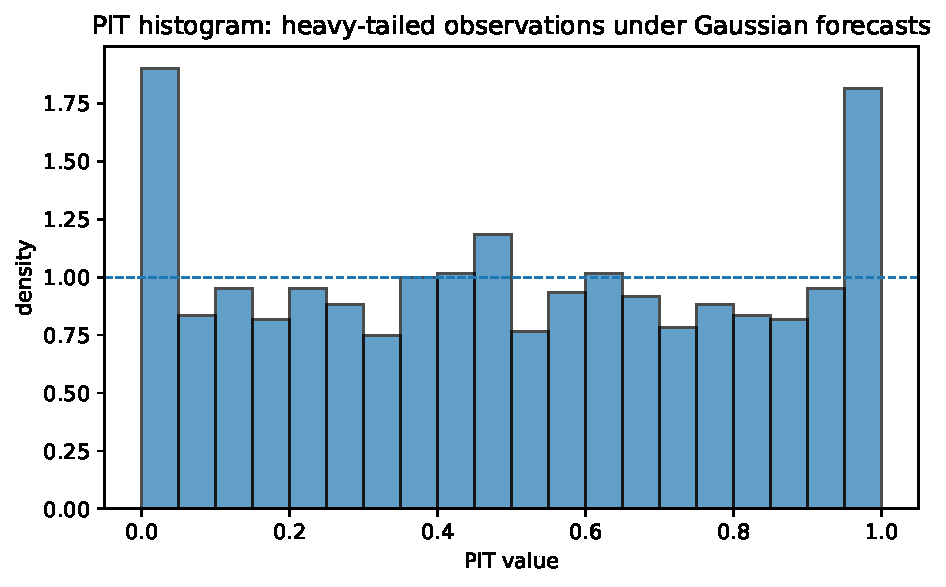
\includegraphics[keepaspectratio]{chapters/chapter-18-probabilistic-forecasting-uncertainty_files/figure-pdf/ch18-pit-diagnostic-output-1.pdf}}

}

\caption{A PIT histogram can reveal forecast distribution
miscalibration.}

\end{figure}%

\section{18.21 Tail risk and decision
thresholds}\label{tail-risk-and-decision-thresholds}

Probabilistic forecasting is especially useful for threshold decisions.
Suppose a decision maker cares whether

\[
Y_{t+h}>c.
\]

A forecast distribution provides

\[
\mathbb P(Y_{t+h}>c\mid\mathcal F_t)=1-F_{t,h}(c).
\]

Examples:

\begin{itemize}
\tightlist
\item
  probability hospital demand exceeds staffed beds;
\item
  probability energy demand exceeds capacity;
\item
  probability inventory demand exceeds stock;
\item
  probability a sensor reading crosses a safety threshold;
\item
  probability revenue falls below a target.
\end{itemize}

The forecast can be connected to expected loss. If under-staffing costs
\(C_u\) and over-staffing costs \(C_o\), the optimal quantile level in a
newsvendor-style problem is

\[
\tau^*=\frac{C_u}{C_u+C_o}.
\]

This is why quantile forecasts are directly decision-relevant.

\section{18.22 Python example: decision threshold
probability}\label{python-example-decision-threshold-probability}

\begin{Shaded}
\begin{Highlighting}[]
\ImportTok{import}\NormalTok{ numpy }\ImportTok{as}\NormalTok{ np}
\ImportTok{import}\NormalTok{ matplotlib.pyplot }\ImportTok{as}\NormalTok{ plt}
\ImportTok{from}\NormalTok{ math }\ImportTok{import}\NormalTok{ erf, sqrt}

\NormalTok{h }\OperatorTok{=}\NormalTok{ np.arange(}\DecValTok{1}\NormalTok{, }\DecValTok{31}\NormalTok{)}
\NormalTok{mu }\OperatorTok{=} \DecValTok{80} \OperatorTok{+} \FloatTok{0.8} \OperatorTok{*}\NormalTok{ h }\OperatorTok{+} \DecValTok{7} \OperatorTok{*}\NormalTok{ np.sin(}\DecValTok{2} \OperatorTok{*}\NormalTok{ np.pi }\OperatorTok{*}\NormalTok{ h }\OperatorTok{/} \DecValTok{14}\NormalTok{)}
\NormalTok{sigma }\OperatorTok{=} \DecValTok{4} \OperatorTok{+} \FloatTok{0.18} \OperatorTok{*}\NormalTok{ h}
\NormalTok{capacity }\OperatorTok{=} \DecValTok{95}

\KeywordTok{def}\NormalTok{ normal\_cdf\_scalar(x):}
    \ControlFlowTok{return} \FloatTok{0.5} \OperatorTok{*}\NormalTok{ (}\DecValTok{1} \OperatorTok{+}\NormalTok{ erf(x }\OperatorTok{/}\NormalTok{ sqrt(}\DecValTok{2}\NormalTok{)))}

\NormalTok{prob\_exceed }\OperatorTok{=}\NormalTok{ np.array([}\DecValTok{1} \OperatorTok{{-}}\NormalTok{ normal\_cdf\_scalar((capacity }\OperatorTok{{-}}\NormalTok{ m) }\OperatorTok{/}\NormalTok{ s) }\ControlFlowTok{for}\NormalTok{ m, s }\KeywordTok{in} \BuiltInTok{zip}\NormalTok{(mu, sigma)])}

\NormalTok{plt.figure(figsize}\OperatorTok{=}\NormalTok{(}\DecValTok{8}\NormalTok{, }\DecValTok{4}\NormalTok{))}
\NormalTok{plt.plot(h, prob\_exceed, marker}\OperatorTok{=}\StringTok{"o"}\NormalTok{)}
\NormalTok{plt.axhline(}\FloatTok{0.5}\NormalTok{, linestyle}\OperatorTok{=}\StringTok{"{-}{-}"}\NormalTok{, linewidth}\OperatorTok{=}\DecValTok{1}\NormalTok{)}
\NormalTok{plt.xlabel(}\StringTok{"forecast horizon"}\NormalTok{)}
\NormalTok{plt.ylabel(}\StringTok{"P(Y exceeds capacity)"}\NormalTok{)}
\NormalTok{plt.title(}\StringTok{"Threshold{-}exceedance probability"}\NormalTok{)}
\NormalTok{plt.ylim(}\DecValTok{0}\NormalTok{, }\DecValTok{1}\NormalTok{)}
\NormalTok{plt.show()}
\end{Highlighting}
\end{Shaded}

\begin{figure}[H]

{\centering \pandocbounded{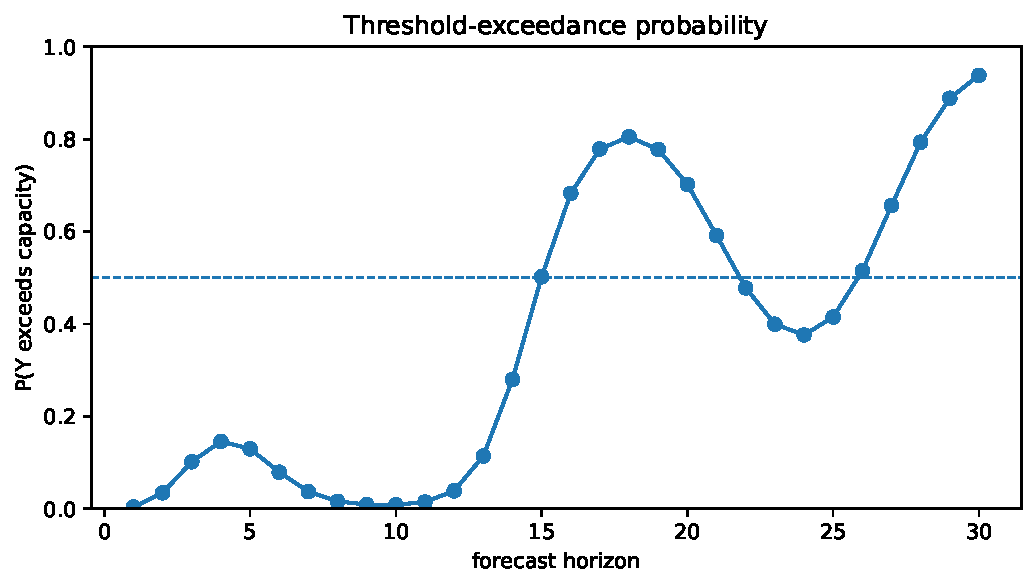
\includegraphics[keepaspectratio]{chapters/chapter-18-probabilistic-forecasting-uncertainty_files/figure-pdf/ch18-threshold-risk-output-1.pdf}}

}

\caption{Forecast distributions can estimate threshold-exceedance
probabilities.}

\end{figure}%

\section{18.23 AI-assisted uncertainty
workflow}\label{ai-assisted-uncertainty-workflow}

\section{Prompt 1: uncertainty model
design}\label{prompt-1-uncertainty-model-design}

Ask:

\begin{quote}
I am forecasting a daily time series with trend, weekly seasonality, and
changing variance. Propose three ways to generate 90\% prediction
intervals: one classical, one machine-learning based, and one conformal.
For each, state the assumptions and diagnostics.
\end{quote}

Check whether the answer respects chronological validation and whether
each method can handle heteroskedasticity.

\section{Prompt 2: coverage audit}\label{prompt-2-coverage-audit}

Ask:

\begin{quote}
Given empirical interval coverage by horizon, interval width by horizon,
and residual plots, diagnose whether my intervals are too narrow, too
wide, biased, or seasonally miscalibrated.
\end{quote}

Then use code to verify every claim.

\section{Prompt 3: decision-focused
forecast}\label{prompt-3-decision-focused-forecast}

Ask:

\begin{quote}
The decision maker cares about the probability that demand exceeds
capacity. Should I optimize RMSE, pinball loss, log score, or
threshold-weighted loss? Explain the tradeoff.
\end{quote}

Use this as a starting point for selecting an evaluation metric.

\section{18.24 Common mistakes}\label{common-mistakes-17}

\begin{enumerate}
\def\labelenumi{\arabic{enumi}.}
\tightlist
\item
  \textbf{Reporting only RMSE.} RMSE says little about uncertainty
  calibration.
\item
  \textbf{Using confidence intervals instead of prediction intervals.}
  Prediction intervals must include future observation noise.
\item
  \textbf{Random calibration split.} This can leak future regimes into
  calibration.
\item
  \textbf{Ignoring horizon.} Coverage often deteriorates at longer
  horizons.
\item
  \textbf{Assuming Gaussian residuals without checking.} Heavy tails and
  skewness matter for intervals.
\item
  \textbf{Using training residuals for calibration.} Training residuals
  are often too optimistic.
\item
  \textbf{Forgetting exogenous uncertainty.} Future covariates may
  themselves need forecasts.
\item
  \textbf{Ignoring heteroskedasticity.} Constant-width intervals fail
  when uncertainty changes with level, season, or regime.
\item
  \textbf{Overtrusting ensemble spread.} Ensemble spread is not the same
  as total predictive uncertainty.
\item
  \textbf{Not connecting uncertainty to decisions.} A 90\% interval may
  not be the right object for an asymmetric-cost problem.
\end{enumerate}

\section{18.25 Mini project: calibrated probabilistic
forecast}\label{mini-project-calibrated-probabilistic-forecast}

Choose a time series with a meaningful forecast horizon. Build and
evaluate at least two probabilistic forecasting methods.

Your report should include:

\begin{enumerate}
\def\labelenumi{\arabic{enumi}.}
\tightlist
\item
  problem statement and decision context;
\item
  train/calibration/test split using chronological order;
\item
  point-forecast baseline;
\item
  at least two uncertainty methods, such as Gaussian intervals, residual
  bootstrap, quantile regression, or conformal intervals;
\item
  empirical coverage by horizon;
\item
  average interval width by horizon;
\item
  residual or PIT-style diagnostic;
\item
  interval examples on a time plot;
\item
  discussion of calibration versus sharpness;
\item
  recommendation for deployment.
\end{enumerate}

Suggested data sets include electricity demand, ridership, website
traffic, retail demand, call-center arrivals, weather, or synthetic data
with controlled heteroskedasticity.

\section{18.26 Exercises}\label{exercises-17}

\begin{enumerate}
\def\labelenumi{\arabic{enumi}.}
\tightlist
\item
  \textbf{Gaussian interval.} Derive the 95\% prediction interval for
  \(Y_{t+h}\mid\mathcal F_t\sim N(\mu_{t,h},\sigma_{t,h}^2)\).
\item
  \textbf{AR(1) uncertainty.} For \(Y_t=\phi Y_{t-1}+W_t\), derive the
  \(h\)-step forecast variance.
\item
  \textbf{Coverage calculation.} Given ten prediction intervals and ten
  outcomes, compute empirical coverage and average width.
\item
  \textbf{Pinball loss.} Prove that the minimizer of expected pinball
  loss is a conditional quantile.
\item
  \textbf{Interval score.} Compute the Winkler interval score for three
  cases: observation inside, below, and above the interval.
\item
  \textbf{Bootstrap interval.} Implement residual-quantile intervals for
  a lagged ridge model.
\item
  \textbf{Conformal quantile.} For calibration scores
  \(s_1,\ldots,s_n\), compute the finite-sample conformal quantile for
  \(\alpha=0.1\).
\item
  \textbf{Time-series calibration.} Explain why random split conformal
  is risky for time-series forecasting.
\item
  \textbf{PIT interpretation.} Sketch what PIT histograms might look
  like when intervals are too narrow, too wide, or biased.
\item
  \textbf{Decision threshold.} Given a forecast distribution, compute
  \(\mathbb P(Y_{t+h}>c\mid\mathcal F_t)\) and describe how it changes
  the decision.
\item
  \textbf{Quantile crossing.} Simulate two independently fitted quantile
  models and check whether crossings occur.
\item
  \textbf{AI critique.} Ask an AI assistant to explain why your forecast
  intervals miss too often. Identify which claims are testable and which
  are speculation.
\end{enumerate}

\section{18.27 Chapter checklist}\label{chapter-checklist-14}

Before moving on, make sure you can:

\begin{itemize}
\tightlist
\item[$\square$]
  define a probabilistic forecast as a conditional distribution;
\item[$\square$]
  distinguish conditional mean, median, and quantiles;
\item[$\square$]
  construct central prediction intervals from quantiles;
\item[$\square$]
  compute Gaussian prediction intervals;
\item[$\square$]
  compute empirical coverage and average interval width;
\item[$\square$]
  explain calibration and sharpness;
\item[$\square$]
  use pinball loss for quantile forecasts;
\item[$\square$]
  use residual quantiles for bootstrap-style intervals;
\item[$\square$]
  construct a split conformal interval with chronological calibration;
\item[$\square$]
  diagnose uncertainty by horizon and regime;
\item[$\square$]
  connect probabilistic forecasts to threshold decisions;
\item[$\square$]
  use AI-generated uncertainty suggestions only after checking
  assumptions and validation.
\end{itemize}

\section{18.28 Companion Python lab}\label{companion-python-lab-1}

Open the companion notebook:
\href{../labs/chapter-18-probabilistic-forecasting-uncertainty-lab.ipynb}{\texttt{chapter-18-probabilistic-forecasting-uncertainty-lab.ipynb}}.

The lab asks you to compare Gaussian, residual-bootstrap,
quantile-regression, and conformal intervals on a synthetic or real time
series; evaluate empirical coverage and average width by horizon; and
write a short uncertainty-audit report.

\part{Part VI. Deep Learning for Time Series and Sequence Data}

\chapter{Neural Networks for Time
Series}\label{neural-networks-for-time-series}

\textbf{Part VI. Deep Learning for Time Series and Sequence Data}\\
\textbf{Chapter goal:} build the first deep-learning forecasting model
for time series by converting ordered observations into supervised
learning examples. We study sliding windows, neural-network maps, loss
functions, backpropagation, regularization, leakage-aware validation,
and AI-assisted model critique.

\section{Learning objectives}\label{learning-objectives-18}

After studying this chapter, you should be able to:

\begin{enumerate}
\def\labelenumi{\arabic{enumi}.}
\tightlist
\item
  convert a univariate or multivariate time series into input-label
  windows;
\item
  distinguish sequence-to-one, sequence-to-sequence, recursive, direct,
  and multi-output neural forecasts;
\item
  define a neural forecasting model as a nonlinear map \(f_\theta\) from
  a history window to a future horizon;
\item
  formulate empirical risk minimization for time-series forecasting;
\item
  explain how backpropagation computes gradients through a computational
  graph;
\item
  train a window-based multilayer perceptron while avoiding time
  leakage;
\item
  compare a neural forecast with naive and linear baselines;
\item
  diagnose overfitting using training and validation loss curves;
\item
  explain why scaling, chronological splitting, and baselines are
  essential;
\item
  use AI tools to critique the modeling workflow while verifying the
  mathematics and code independently.
\end{enumerate}

\section{19.1 From classical forecasts to neural sequence
maps}\label{from-classical-forecasts-to-neural-sequence-maps}

Classical models in earlier chapters describe the current observation
using explicit stochastic structure. For example, an AR(\(p\)) model has
the form

\[
Y_t = \phi_1Y_{t-1}+\cdots+\phi_pY_{t-p}+W_t.
\]

The one-step conditional mean is linear in the past:

\[
\mathbb E[Y_t\mid Y_{t-1},\ldots,Y_{t-p}]
=
\phi_1Y_{t-1}+\cdots+\phi_pY_{t-p}.
\]

A neural time-series model keeps the forecasting viewpoint but replaces
the explicit linear map by a learned nonlinear map. Given a history
window

\[
\mathbf x_t=(Y_{t-L+1},Y_{t-L+2},\ldots,Y_t)\in\mathbb R^L,
\]

and a forecasting horizon \(H\), the target vector is

\[
\mathbf y_t=(Y_{t+1},Y_{t+2},\ldots,Y_{t+H})\in\mathbb R^H.
\]

A neural forecasting model is a parameterized function

\[
f_\theta:\mathbb R^L\to\mathbb R^H,
\qquad
\widehat{\mathbf y}_t=f_\theta(\mathbf x_t).
\]

This framework generalizes the AR model. If \(H=1\) and \(f_\theta\) is
linear, then the model is essentially an autoregression estimated by
supervised learning. If \(f_\theta\) is a multilayer neural network, it
can learn nonlinear interactions among lags.

\begin{tcolorbox}[enhanced jigsaw, arc=.35mm, bottomrule=.15mm, bottomtitle=1mm, breakable, colback=white, colbacktitle=quarto-callout-note-color!10!white, colframe=quarto-callout-note-color-frame, coltitle=black, left=2mm, leftrule=.75mm, opacityback=0, opacitybacktitle=0.6, rightrule=.15mm, title=\textcolor{quarto-callout-note-color}{\faInfo}\hspace{0.5em}{Neural forecasting is still forecasting}, titlerule=0mm, toprule=.15mm, toptitle=1mm]

Deep learning does not remove the need for time-series thinking. We
still need baselines, chronological validation, horizon-specific error
analysis, and diagnostics for failures.

\end{tcolorbox}

\section{19.2 Time-series windows as supervised learning
data}\label{time-series-windows-as-supervised-learning-data}

Suppose we observe a sequence

\[
Y_1,Y_2,\ldots,Y_T.
\]

Choose an input length \(L\) and forecast horizon \(H\). For each
feasible forecast origin \(t\), construct

\[
\mathbf x_t=(Y_{t-L+1},\ldots,Y_t)
\]

and

\[
\mathbf y_t=(Y_{t+1},\ldots,Y_{t+H}).
\]

The resulting supervised data set is

\[
\mathcal D
=
\{(\mathbf x_t,\mathbf y_t):L\le t\le T-H\}.
\]

Equivalently, the design matrix has rows

\[
X=
\begin{bmatrix}
Y_1 & Y_2 & \cdots & Y_L\\
Y_2 & Y_3 & \cdots & Y_{L+1}\\
\vdots & \vdots & \ddots & \vdots\\
Y_{T-L-H+1} & Y_{T-L-H+2} & \cdots & Y_{T-H}
\end{bmatrix},
\]

and the target matrix is

\[
Z=
\begin{bmatrix}
Y_{L+1} & Y_{L+2} & \cdots & Y_{L+H}\\
Y_{L+2} & Y_{L+3} & \cdots & Y_{L+H+1}\\
\vdots & \vdots & \ddots & \vdots\\
Y_{T-H+1} & Y_{T-H+2} & \cdots & Y_T
\end{bmatrix}.
\]

Each row is one supervised example. The row order is temporal and must
be respected during validation.

\subsection{Sequence-to-one and
sequence-to-sequence}\label{sequence-to-one-and-sequence-to-sequence}

A \textbf{sequence-to-one} model uses a history window to forecast one
future value:

\[
f_\theta:\mathbb R^L\to\mathbb R,
\qquad
\widehat Y_{t+1}=f_\theta(Y_{t-L+1},\ldots,Y_t).
\]

A \textbf{sequence-to-sequence} or \textbf{multi-output} model forecasts
several future values at once:

\[
f_\theta:\mathbb R^L\to\mathbb R^H,
\qquad
(\widehat Y_{t+1},\ldots,\widehat Y_{t+H})=f_\theta(\mathbf x_t).
\]

For multivariate time series \(\mathbf Y_t\in\mathbb R^d\), the input
window is a matrix

\[
\mathbf X_t=
\begin{bmatrix}
\mathbf Y_{t-L+1}^\top\\
\mathbf Y_{t-L+2}^\top\\
\vdots\\
\mathbf Y_t^\top
\end{bmatrix}
\in\mathbb R^{L\times d}.
\]

An MLP usually flattens this matrix into a vector in \(\mathbb R^{Ld}\).
Later chapters will preserve the temporal geometry using convolutional,
recurrent, and attention-based architectures.

\section{19.3 Direct, recursive, and multi-output neural
forecasts}\label{direct-recursive-and-multi-output-neural-forecasts}

There are several ways to forecast multiple steps ahead.

\subsection{Recursive one-step
strategy}\label{recursive-one-step-strategy}

Train a one-step model

\[
\widehat Y_{t+1}=f_\theta(Y_{t-L+1},\ldots,Y_t),
\]

then feed its own forecast back into the input window:

\[
\widehat Y_{t+2}=f_\theta(Y_{t-L+2},\ldots,Y_t,\widehat Y_{t+1}).
\]

This is simple, but errors can accumulate.

\subsection{Direct strategy}\label{direct-strategy-2}

Train a separate model for each horizon:

\[
\widehat Y_{t+h}=f_{\theta_h}^{(h)}(Y_{t-L+1},\ldots,Y_t),
\qquad h=1,\ldots,H.
\]

This avoids recursive error propagation but requires fitting \(H\)
models.

\subsection{Multi-output strategy}\label{multi-output-strategy-2}

Train one model that outputs all horizons simultaneously:

\[
(\widehat Y_{t+1},\ldots,\widehat Y_{t+H})
=
f_\theta(Y_{t-L+1},\ldots,Y_t).
\]

This is the strategy used in the main Python example below. It
encourages the model to learn a coherent future path.

\section{Neural networks as nonlinear
autoregressions}\label{neural-networks-as-nonlinear-autoregressions}

A window-based neural forecast can be viewed as a nonlinear
autoregressive model:

\[
Y_{t+1}=f_\theta(Y_t,Y_{t-1},\ldots,Y_{t-L+1})+\varepsilon_{t+1}.
\]

The model is not automatically better than ARIMA or SARIMA. Its
advantage appears when nonlinear lag interactions, many covariates, or
complex regime-dependent effects are important and enough data are
available.

\section{19.4 Mathematical form of a multilayer
perceptron}\label{mathematical-form-of-a-multilayer-perceptron}

A feedforward neural network is a composition of affine maps and
nonlinear activation functions. Let

\[
\mathbf h^{(0)}=\mathbf x.
\]

For layers \(\ell=1,\ldots,m\), define

\[
\mathbf a^{(\ell)}=W^{(\ell)}\mathbf h^{(\ell-1)}+\mathbf b^{(\ell)},
\]

and

\[
\mathbf h^{(\ell)}=\sigma_\ell(\mathbf a^{(\ell)}).
\]

For a regression forecast, the final layer is often linear:

\[
f_\theta(\mathbf x)
=
W^{(m+1)}\mathbf h^{(m)}+\mathbf b^{(m+1)}.
\]

The full parameter vector is

\[
\theta=
\{W^{(1)},\mathbf b^{(1)},\ldots,W^{(m+1)},\mathbf b^{(m+1)}\}.
\]

Common activations include:

\[
\operatorname{ReLU}(z)=\max\{0,z\},
\]

\[
\tanh(z)=\frac{e^z-e^{-z}}{e^z+e^{-z}},
\]

and

\[
\sigma(z)=\frac{1}{1+e^{-z}}.
\]

The activation function is what makes the model nonlinear. Without
nonlinear activations, a composition of affine transformations collapses
to a single affine transformation.

\section{19.5 Loss functions and empirical
risk}\label{loss-functions-and-empirical-risk}

Let \(\mathcal I_{\text{train}}\) be the set of training forecast
origins. For a multi-output forecast with horizon \(H\), the mean
squared error objective is

\[
J(\theta)
=
\frac{1}{|\mathcal I_{\text{train}}|H}
\sum_{t\in\mathcal I_{\text{train}}}
\sum_{h=1}^H
\left(Y_{t+h}-\widehat Y_{t+h|t}\right)^2,
\]

where

\[
(\widehat Y_{t+1|t},\ldots,\widehat Y_{t+H|t})=f_\theta(\mathbf x_t).
\]

Other losses may be better for different goals:

\begin{itemize}
\tightlist
\item
  mean absolute error for robustness;
\item
  Huber loss for a compromise between MSE and MAE;
\item
  quantile loss for probabilistic forecasting;
\item
  cross-entropy for sequence classification;
\item
  custom decision loss when underprediction and overprediction have
  different costs.
\end{itemize}

With \(L_2\) regularization, the training problem becomes

\[
\widehat\theta
=
\arg\min_\theta
\left\{
J(\theta)+\lambda\|\theta\|_2^2
\right\}.
\]

In neural-network terminology, \(\lambda\|\theta\|_2^2\) is often
implemented as \textbf{weight decay}.

\section{19.6 Backpropagation as the chain rule on a computational
graph}\label{backpropagation-as-the-chain-rule-on-a-computational-graph}

Training requires gradients of the loss with respect to all parameters:

\[
\nabla_\theta J(\theta).
\]

For a one-hidden-layer network,

\[
\widehat y
=
\mathbf v^\top \sigma(W\mathbf x+\mathbf b)+c,
\]

and squared loss

\[
L(\theta)=\frac12(\widehat y-y)^2,
\]

we can write the computation as

\[
\mathbf a=W\mathbf x+\mathbf b,
\qquad
\mathbf h=\sigma(\mathbf a),
\qquad
\widehat y=\mathbf v^\top\mathbf h+c,
\qquad
L=\frac12(\widehat y-y)^2.
\]

The chain rule gives

\[
\frac{\partial L}{\partial \widehat y}=\widehat y-y,
\]

\[
\frac{\partial L}{\partial \mathbf v}
=(\widehat y-y)\mathbf h,
\qquad
\frac{\partial L}{\partial c}=\widehat y-y,
\]

and

\[
\frac{\partial L}{\partial W}
=
\left[(\widehat y-y)\mathbf v\odot \sigma'(\mathbf a)\right]\mathbf x^\top,
\]

\[
\frac{\partial L}{\partial \mathbf b}
=(\widehat y-y)\mathbf v\odot \sigma'(\mathbf a).
\]

Backpropagation is an efficient algorithmic procedure for applying these
chain-rule calculations through a large computational graph. It is not
finite-difference differentiation, and it is not symbolic
simplification. It stores intermediate quantities from the forward pass
and reuses them in the backward pass.

Gradient descent updates parameters by

\[
\theta_{k+1}=\theta_k-\alpha\nabla_\theta J(\theta_k),
\]

or, in practice, by a stochastic or mini-batch variant such as Adam or
AdamW.

\begin{tcolorbox}[enhanced jigsaw, arc=.35mm, bottomrule=.15mm, bottomtitle=1mm, breakable, colback=white, colbacktitle=quarto-callout-note-color!10!white, colframe=quarto-callout-note-color-frame, coltitle=black, left=2mm, leftrule=.75mm, opacityback=0, opacitybacktitle=0.6, rightrule=.15mm, title=\textcolor{quarto-callout-note-color}{\faInfo}\hspace{0.5em}{Why this matters for time series}, titlerule=0mm, toprule=.15mm, toptitle=1mm]

For a time-series neural network, the inputs are not independent in
time. But once windows are constructed, the training objective is still
an empirical risk over many overlapping examples. The validation design
must remember where those windows came from.

\end{tcolorbox}

\section{19.7 Interactive demonstration: input and label
windows}\label{interactive-demonstration-input-and-label-windows}

The module below shows how a single observed series is transformed into
supervised examples. The blue points form the input window and the
orange points form the label window.

Interactive Module: Sliding Window Builder

Change the input length, forecast horizon, and window start. The maximum
start value is adjusted automatically so the input and label windows
always fit inside the simulated series.

\begin{verbatim}
<label for="ch19_input"><strong>Input length $L$:</strong> <span id="ch19_input_value">24</span></label>
<input id="ch19_input" type="range" min="6" max="36" step="1" value="24">

<label for="ch19_horizon"><strong>Forecast horizon $H$:</strong> <span id="ch19_horizon_value">12</span></label>
<input id="ch19_horizon" type="range" min="1" max="24" step="1" value="12">

<label for="ch19_start"><strong>Window start:</strong> <span id="ch19_start_value">10</span></label>
<input id="ch19_start" type="range" min="0" max="84" step="1" value="10">
\end{verbatim}

\protect\phantomsection\label{ch19_window_plot}

\section{19.8 Interactive demonstration: activation
functions}\label{interactive-demonstration-activation-functions}

Neural networks become nonlinear because of activation functions. The
module below compares three common choices.

Interactive Module: Activation Function Explorer

The activation is applied after an affine transformation. Without it,
stacking layers would still produce only an affine map.

Input scale:
\protect\phantomsection\label{ch19-activation-scale-value}{1.00}

Bias shift:
\protect\phantomsection\label{ch19-activation-bias-value}{0.00}

\protect\phantomsection\label{ch19-activation-plot}

\section{19.9 Python example: simulate a nonlinear seasonal time
series}\label{python-example-simulate-a-nonlinear-seasonal-time-series}

The following synthetic series contains autoregressive dependence,
nonlinear dependence, seasonality, and noise. It is simple enough to
understand but nonlinear enough to motivate a neural model.

\begin{Shaded}
\begin{Highlighting}[]
\ImportTok{import}\NormalTok{ numpy }\ImportTok{as}\NormalTok{ np}
\ImportTok{import}\NormalTok{ pandas }\ImportTok{as}\NormalTok{ pd}
\ImportTok{import}\NormalTok{ matplotlib.pyplot }\ImportTok{as}\NormalTok{ plt}

\NormalTok{rng }\OperatorTok{=}\NormalTok{ np.random.default\_rng(}\DecValTok{7339}\NormalTok{)}

\NormalTok{n }\OperatorTok{=} \DecValTok{650}
\NormalTok{y }\OperatorTok{=}\NormalTok{ np.zeros(n)}

\ControlFlowTok{for}\NormalTok{ t }\KeywordTok{in} \BuiltInTok{range}\NormalTok{(}\DecValTok{2}\NormalTok{, n):}
\NormalTok{    seasonal }\OperatorTok{=} \FloatTok{0.45} \OperatorTok{*}\NormalTok{ np.sin(}\DecValTok{2} \OperatorTok{*}\NormalTok{ np.pi }\OperatorTok{*}\NormalTok{ t }\OperatorTok{/} \DecValTok{24}\NormalTok{)}
\NormalTok{    nonlinear }\OperatorTok{=} \FloatTok{0.25} \OperatorTok{*}\NormalTok{ np.tanh(}\FloatTok{1.5} \OperatorTok{*}\NormalTok{ y[t }\OperatorTok{{-}} \DecValTok{1}\NormalTok{])}
\NormalTok{    y[t] }\OperatorTok{=}\NormalTok{ (}
        \FloatTok{0.62} \OperatorTok{*}\NormalTok{ y[t }\OperatorTok{{-}} \DecValTok{1}\NormalTok{]}
        \OperatorTok{{-}} \FloatTok{0.22} \OperatorTok{*}\NormalTok{ y[t }\OperatorTok{{-}} \DecValTok{2}\NormalTok{]}
        \OperatorTok{+}\NormalTok{ seasonal}
        \OperatorTok{+}\NormalTok{ nonlinear}
        \OperatorTok{+}\NormalTok{ rng.normal(}\DecValTok{0}\NormalTok{, }\FloatTok{0.28}\NormalTok{)}
\NormalTok{    )}

\NormalTok{time }\OperatorTok{=}\NormalTok{ np.arange(n)}

\NormalTok{plt.figure(figsize}\OperatorTok{=}\NormalTok{(}\DecValTok{9}\NormalTok{, }\DecValTok{4}\NormalTok{))}
\NormalTok{plt.plot(time, y)}
\NormalTok{plt.xlabel(}\StringTok{"time"}\NormalTok{)}
\NormalTok{plt.ylabel(}\StringTok{"value"}\NormalTok{)}
\NormalTok{plt.title(}\StringTok{"Synthetic nonlinear seasonal time series"}\NormalTok{)}
\NormalTok{plt.show()}
\end{Highlighting}
\end{Shaded}

\begin{figure}[H]

{\centering \pandocbounded{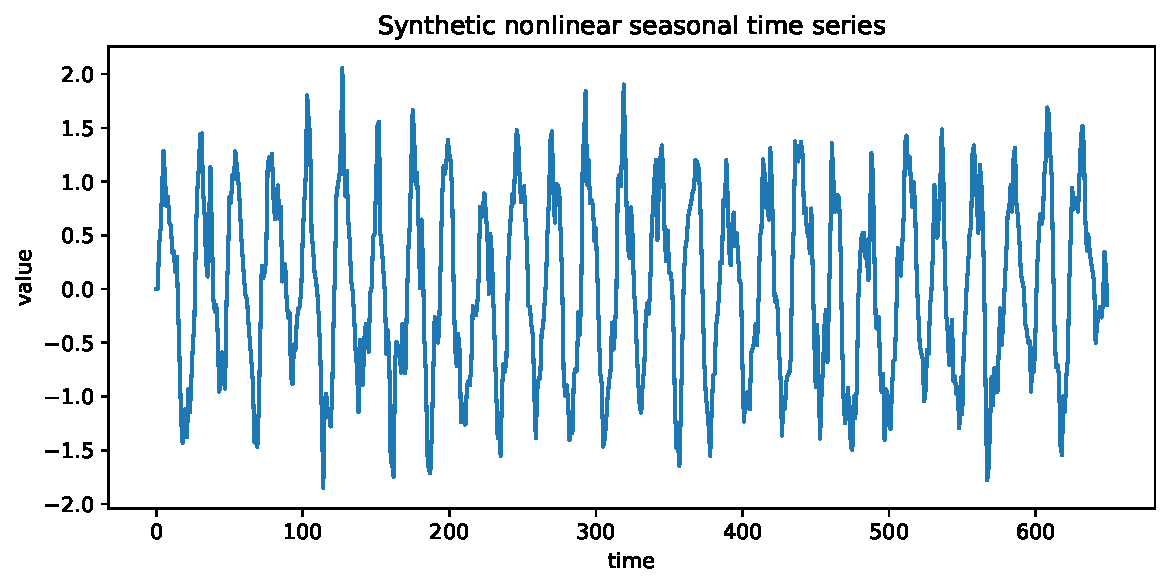
\includegraphics[keepaspectratio]{chapters/chapter-19-neural-networks-for-time-series_files/figure-pdf/ch19-simulate-nonlinear-series-output-1.pdf}}

}

\caption{Synthetic nonlinear seasonal time series for neural
forecasting.}

\end{figure}%

\section{19.10 Python example: construct input and label
windows}\label{python-example-construct-input-and-label-windows}

The function below transforms a single series into a supervised learning
data set. This is the most important preprocessing step for neural
forecasting.

\protect\phantomsection\label{ch19-window-function}
\begin{Shaded}
\begin{Highlighting}[]
\KeywordTok{def}\NormalTok{ make\_windows(series, input\_length, horizon):}
    \CommentTok{"""Return input windows X, target windows Y, and forecast origins.}

\CommentTok{    X[i] contains observations used as input.}
\CommentTok{    Y[i] contains the next horizon observations used as labels.}
\CommentTok{    origins[i] is the last time index included in X[i].}
\CommentTok{    """}
\NormalTok{    series }\OperatorTok{=}\NormalTok{ np.asarray(series, dtype}\OperatorTok{=}\BuiltInTok{float}\NormalTok{)}
\NormalTok{    X, Y, origins }\OperatorTok{=}\NormalTok{ [], [], []}
\NormalTok{    last\_start }\OperatorTok{=} \BuiltInTok{len}\NormalTok{(series) }\OperatorTok{{-}}\NormalTok{ input\_length }\OperatorTok{{-}}\NormalTok{ horizon }\OperatorTok{+} \DecValTok{1}

    \ControlFlowTok{for}\NormalTok{ start }\KeywordTok{in} \BuiltInTok{range}\NormalTok{(last\_start):}
\NormalTok{        end }\OperatorTok{=}\NormalTok{ start }\OperatorTok{+}\NormalTok{ input\_length}
\NormalTok{        X.append(series[start:end])}
\NormalTok{        Y.append(series[end:end }\OperatorTok{+}\NormalTok{ horizon])}
\NormalTok{        origins.append(end }\OperatorTok{{-}} \DecValTok{1}\NormalTok{)}

    \ControlFlowTok{return}\NormalTok{ np.asarray(X), np.asarray(Y), np.asarray(origins)}

\NormalTok{L }\OperatorTok{=} \DecValTok{36}
\NormalTok{H }\OperatorTok{=} \DecValTok{12}
\NormalTok{X, Y, origins }\OperatorTok{=}\NormalTok{ make\_windows(y, input\_length}\OperatorTok{=}\NormalTok{L, horizon}\OperatorTok{=}\NormalTok{H)}

\BuiltInTok{print}\NormalTok{(}\StringTok{"X shape:"}\NormalTok{, X.shape)}
\BuiltInTok{print}\NormalTok{(}\StringTok{"Y shape:"}\NormalTok{, Y.shape)}
\BuiltInTok{print}\NormalTok{(}\StringTok{"First forecast origin:"}\NormalTok{, origins[}\DecValTok{0}\NormalTok{])}
\end{Highlighting}
\end{Shaded}

\begin{verbatim}
X shape: (603, 36)
Y shape: (603, 12)
First forecast origin: 35
\end{verbatim}

\begin{Shaded}
\begin{Highlighting}[]
\NormalTok{example }\OperatorTok{=} \DecValTok{120}
\NormalTok{input\_index }\OperatorTok{=}\NormalTok{ np.arange(example, example }\OperatorTok{+}\NormalTok{ L)}
\NormalTok{label\_index }\OperatorTok{=}\NormalTok{ np.arange(example }\OperatorTok{+}\NormalTok{ L, example }\OperatorTok{+}\NormalTok{ L }\OperatorTok{+}\NormalTok{ H)}

\NormalTok{plt.figure(figsize}\OperatorTok{=}\NormalTok{(}\DecValTok{9}\NormalTok{, }\DecValTok{4}\NormalTok{))}
\NormalTok{plt.plot(time, y, linewidth}\OperatorTok{=}\DecValTok{1}\NormalTok{, label}\OperatorTok{=}\StringTok{"full series"}\NormalTok{)}
\NormalTok{plt.scatter(input\_index, y[input\_index], label}\OperatorTok{=}\StringTok{"input window"}\NormalTok{, zorder}\OperatorTok{=}\DecValTok{3}\NormalTok{)}
\NormalTok{plt.scatter(label\_index, y[label\_index], marker}\OperatorTok{=}\StringTok{"x"}\NormalTok{, s}\OperatorTok{=}\DecValTok{70}\NormalTok{, label}\OperatorTok{=}\StringTok{"label window"}\NormalTok{, zorder}\OperatorTok{=}\DecValTok{3}\NormalTok{)}
\NormalTok{plt.xlabel(}\StringTok{"time"}\NormalTok{)}
\NormalTok{plt.ylabel(}\StringTok{"value"}\NormalTok{)}
\NormalTok{plt.title(}\StringTok{"A supervised example produced from a time series"}\NormalTok{)}
\NormalTok{plt.legend()}
\NormalTok{plt.show()}
\end{Highlighting}
\end{Shaded}

\begin{figure}[H]

{\centering \pandocbounded{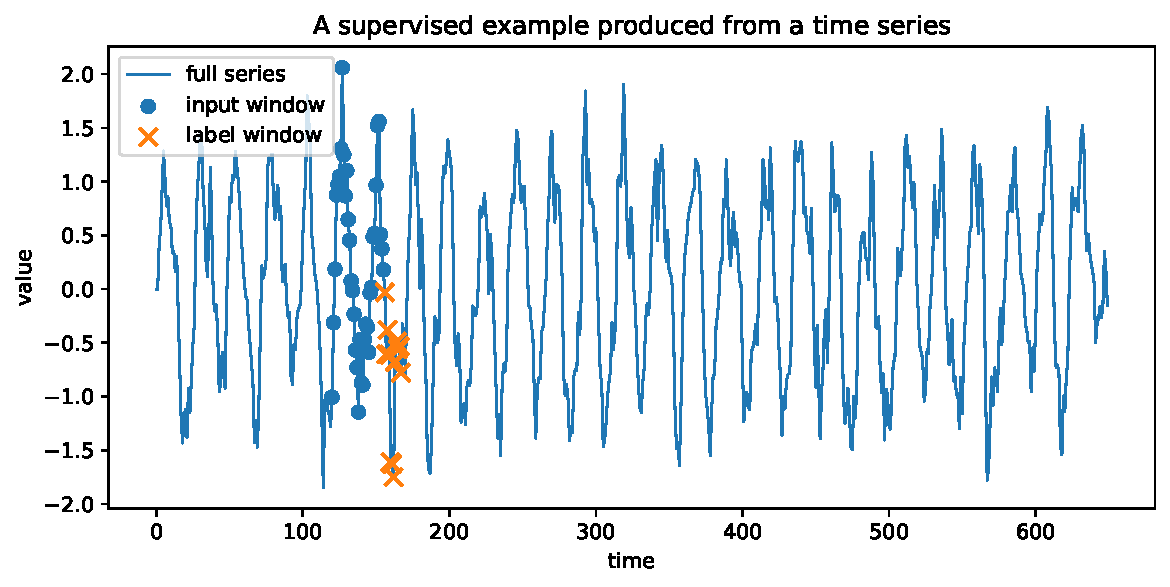
\includegraphics[keepaspectratio]{chapters/chapter-19-neural-networks-for-time-series_files/figure-pdf/ch19-window-visualization-output-1.pdf}}

}

\caption{One input window and its corresponding label window.}

\end{figure}%

\section{19.11 Chronological splitting and
scaling}\label{chronological-splitting-and-scaling}

A random split is usually invalid for forecasting because it lets future
patterns leak into the training set. We split the windowed examples
chronologically:

\[
\text{train} \; \longrightarrow \; \text{validation} \; \longrightarrow \; \text{test}.
\]

Scaling must also be fit on the training period only. If the test period
is used to compute the mean or standard deviation, the model has already
seen information from the future.

\protect\phantomsection\label{ch19-split-scale}
\begin{Shaded}
\begin{Highlighting}[]
\ImportTok{from}\NormalTok{ sklearn.preprocessing }\ImportTok{import}\NormalTok{ StandardScaler}

\NormalTok{train\_end }\OperatorTok{=} \BuiltInTok{int}\NormalTok{(}\FloatTok{0.70} \OperatorTok{*} \BuiltInTok{len}\NormalTok{(X))}
\NormalTok{val\_end }\OperatorTok{=} \BuiltInTok{int}\NormalTok{(}\FloatTok{0.85} \OperatorTok{*} \BuiltInTok{len}\NormalTok{(X))}

\NormalTok{X\_train, Y\_train }\OperatorTok{=}\NormalTok{ X[:train\_end], Y[:train\_end]}
\NormalTok{X\_val, Y\_val }\OperatorTok{=}\NormalTok{ X[train\_end:val\_end], Y[train\_end:val\_end]}
\NormalTok{X\_test, Y\_test }\OperatorTok{=}\NormalTok{ X[val\_end:], Y[val\_end:]}

\NormalTok{x\_scaler }\OperatorTok{=}\NormalTok{ StandardScaler().fit(X\_train)}
\NormalTok{y\_scaler }\OperatorTok{=}\NormalTok{ StandardScaler().fit(Y\_train)}

\NormalTok{Xs\_train }\OperatorTok{=}\NormalTok{ x\_scaler.transform(X\_train)}
\NormalTok{Xs\_val }\OperatorTok{=}\NormalTok{ x\_scaler.transform(X\_val)}
\NormalTok{Xs\_test }\OperatorTok{=}\NormalTok{ x\_scaler.transform(X\_test)}

\NormalTok{Ys\_train }\OperatorTok{=}\NormalTok{ y\_scaler.transform(Y\_train)}
\NormalTok{Ys\_val }\OperatorTok{=}\NormalTok{ y\_scaler.transform(Y\_val)}
\NormalTok{Ys\_test }\OperatorTok{=}\NormalTok{ y\_scaler.transform(Y\_test)}

\BuiltInTok{print}\NormalTok{(}\StringTok{"Number of training windows:"}\NormalTok{, }\BuiltInTok{len}\NormalTok{(X\_train))}
\BuiltInTok{print}\NormalTok{(}\StringTok{"Number of validation windows:"}\NormalTok{, }\BuiltInTok{len}\NormalTok{(X\_val))}
\BuiltInTok{print}\NormalTok{(}\StringTok{"Number of test windows:"}\NormalTok{, }\BuiltInTok{len}\NormalTok{(X\_test))}
\end{Highlighting}
\end{Shaded}

\begin{verbatim}
Number of training windows: 422
Number of validation windows: 90
Number of test windows: 91
\end{verbatim}

\begin{tcolorbox}[enhanced jigsaw, arc=.35mm, bottomrule=.15mm, bottomtitle=1mm, breakable, colback=white, colbacktitle=quarto-callout-warning-color!10!white, colframe=quarto-callout-warning-color-frame, coltitle=black, left=2mm, leftrule=.75mm, opacityback=0, opacitybacktitle=0.6, rightrule=.15mm, title=\textcolor{quarto-callout-warning-color}{\faExclamationTriangle}\hspace{0.5em}{Scaling leakage}, titlerule=0mm, toprule=.15mm, toptitle=1mm]

Do not call \texttt{fit\_transform} on the full data set before
splitting. For forecasting, preprocessing parameters should be learned
from the training period and then applied to validation and test
periods.

\end{tcolorbox}

\section{19.12 Python example: baseline and linear window
models}\label{python-example-baseline-and-linear-window-models}

Before training a neural network, always build baselines. A useful naive
multi-step forecast repeats the most recent observed value:

\[
\widehat Y_{t+h|t}=Y_t,
\qquad h=1,\ldots,H.
\]

We also fit a ridge regression model on the same input windows. This is
a linear benchmark for the neural network.

\begin{Shaded}
\begin{Highlighting}[]
\ImportTok{from}\NormalTok{ sklearn.linear\_model }\ImportTok{import}\NormalTok{ Ridge}
\ImportTok{from}\NormalTok{ sklearn.metrics }\ImportTok{import}\NormalTok{ mean\_absolute\_error, mean\_squared\_error}

\NormalTok{naive\_pred }\OperatorTok{=}\NormalTok{ np.repeat(X\_test[:, }\OperatorTok{{-}}\DecValTok{1}\NormalTok{:], H, axis}\OperatorTok{=}\DecValTok{1}\NormalTok{)}

\NormalTok{ridge }\OperatorTok{=}\NormalTok{ Ridge(alpha}\OperatorTok{=}\FloatTok{3.0}\NormalTok{)}
\NormalTok{ridge.fit(Xs\_train, Ys\_train)}
\NormalTok{ridge\_pred\_scaled }\OperatorTok{=}\NormalTok{ ridge.predict(Xs\_test)}
\NormalTok{ridge\_pred }\OperatorTok{=}\NormalTok{ y\_scaler.inverse\_transform(ridge\_pred\_scaled)}

\KeywordTok{def}\NormalTok{ forecast\_metrics(name, truth, pred):}
\NormalTok{    truth\_flat }\OperatorTok{=}\NormalTok{ truth.ravel()}
\NormalTok{    pred\_flat }\OperatorTok{=}\NormalTok{ pred.ravel()}
\NormalTok{    rmse }\OperatorTok{=}\NormalTok{ np.sqrt(mean\_squared\_error(truth\_flat, pred\_flat))}
\NormalTok{    mae }\OperatorTok{=}\NormalTok{ mean\_absolute\_error(truth\_flat, pred\_flat)}
    \ControlFlowTok{return}\NormalTok{ \{}\StringTok{"model"}\NormalTok{: name, }\StringTok{"RMSE"}\NormalTok{: rmse, }\StringTok{"MAE"}\NormalTok{: mae\}}

\NormalTok{baseline\_results }\OperatorTok{=}\NormalTok{ [}
\NormalTok{    forecast\_metrics(}\StringTok{"naive repeat{-}last"}\NormalTok{, Y\_test, naive\_pred),}
\NormalTok{    forecast\_metrics(}\StringTok{"ridge window model"}\NormalTok{, Y\_test, ridge\_pred),}
\NormalTok{]}

\NormalTok{pd.DataFrame(baseline\_results)}
\end{Highlighting}
\end{Shaded}

\protect\phantomsection\label{ch19-baselines}
{\def\LTcaptype{none} % do not increment counter
\begin{longtable}[]{@{}llll@{}}
\toprule\noalign{}
& model & RMSE & MAE \\
\midrule\noalign{}
\endhead
\bottomrule\noalign{}
\endlastfoot
0 & naive repeat-last & 1.236725 & 1.009598 \\
1 & ridge window model & 0.499328 & 0.404376 \\
\end{longtable}
}

\section{19.13 Python example: train a window-based MLP in
PyTorch}\label{python-example-train-a-window-based-mlp-in-pytorch}

The MLP below maps an input window of length \(L=36\) to a forecast path
of length \(H=12\):

\[
f_\theta:\mathbb R^{36}\to\mathbb R^{12}.
\]

The architecture is intentionally small. In a course project, model size
should be chosen by validation performance, not by excitement about deep
learning.

\begin{Shaded}
\begin{Highlighting}[]
\ImportTok{import}\NormalTok{ torch}
\ImportTok{from}\NormalTok{ torch }\ImportTok{import}\NormalTok{ nn}

\NormalTok{torch.manual\_seed(}\DecValTok{7339}\NormalTok{)}
\NormalTok{torch.set\_num\_threads(}\DecValTok{1}\NormalTok{)}

\NormalTok{Xtr }\OperatorTok{=}\NormalTok{ torch.tensor(Xs\_train, dtype}\OperatorTok{=}\NormalTok{torch.float32)}
\NormalTok{Ytr }\OperatorTok{=}\NormalTok{ torch.tensor(Ys\_train, dtype}\OperatorTok{=}\NormalTok{torch.float32)}
\NormalTok{Xva }\OperatorTok{=}\NormalTok{ torch.tensor(Xs\_val, dtype}\OperatorTok{=}\NormalTok{torch.float32)}
\NormalTok{Yva }\OperatorTok{=}\NormalTok{ torch.tensor(Ys\_val, dtype}\OperatorTok{=}\NormalTok{torch.float32)}

\KeywordTok{class}\NormalTok{ WindowMLP(nn.Module):}
    \KeywordTok{def} \FunctionTok{\_\_init\_\_}\NormalTok{(}\VariableTok{self}\NormalTok{, input\_length, horizon):}
        \BuiltInTok{super}\NormalTok{().}\FunctionTok{\_\_init\_\_}\NormalTok{()}
        \VariableTok{self}\NormalTok{.net }\OperatorTok{=}\NormalTok{ nn.Sequential(}
\NormalTok{            nn.Linear(input\_length, }\DecValTok{64}\NormalTok{),}
\NormalTok{            nn.ReLU(),}
\NormalTok{            nn.Dropout(}\FloatTok{0.10}\NormalTok{),}
\NormalTok{            nn.Linear(}\DecValTok{64}\NormalTok{, }\DecValTok{32}\NormalTok{),}
\NormalTok{            nn.ReLU(),}
\NormalTok{            nn.Linear(}\DecValTok{32}\NormalTok{, horizon),}
\NormalTok{        )}

    \KeywordTok{def}\NormalTok{ forward(}\VariableTok{self}\NormalTok{, x):}
        \ControlFlowTok{return} \VariableTok{self}\NormalTok{.net(x)}

\NormalTok{model }\OperatorTok{=}\NormalTok{ WindowMLP(input\_length}\OperatorTok{=}\NormalTok{L, horizon}\OperatorTok{=}\NormalTok{H)}
\NormalTok{loss\_fn }\OperatorTok{=}\NormalTok{ nn.MSELoss()}
\NormalTok{optimizer }\OperatorTok{=}\NormalTok{ torch.optim.AdamW(model.parameters(), lr}\OperatorTok{=}\FloatTok{1e{-}3}\NormalTok{, weight\_decay}\OperatorTok{=}\FloatTok{1e{-}3}\NormalTok{)}

\NormalTok{train\_losses }\OperatorTok{=}\NormalTok{ []}
\NormalTok{val\_losses }\OperatorTok{=}\NormalTok{ []}
\NormalTok{best\_state }\OperatorTok{=} \VariableTok{None}
\NormalTok{best\_val }\OperatorTok{=} \BuiltInTok{float}\NormalTok{(}\StringTok{"inf"}\NormalTok{)}
\NormalTok{patience }\OperatorTok{=} \DecValTok{30}
\NormalTok{wait }\OperatorTok{=} \DecValTok{0}

\ControlFlowTok{for}\NormalTok{ epoch }\KeywordTok{in} \BuiltInTok{range}\NormalTok{(}\DecValTok{300}\NormalTok{):}
\NormalTok{    model.train()}
\NormalTok{    optimizer.zero\_grad()}
\NormalTok{    pred }\OperatorTok{=}\NormalTok{ model(Xtr)}
\NormalTok{    loss }\OperatorTok{=}\NormalTok{ loss\_fn(pred, Ytr)}
\NormalTok{    loss.backward()}
\NormalTok{    optimizer.step()}

\NormalTok{    model.}\BuiltInTok{eval}\NormalTok{()}
    \ControlFlowTok{with}\NormalTok{ torch.no\_grad():}
\NormalTok{        val\_loss }\OperatorTok{=}\NormalTok{ loss\_fn(model(Xva), Yva).item()}

\NormalTok{    train\_losses.append(loss.item())}
\NormalTok{    val\_losses.append(val\_loss)}

    \ControlFlowTok{if}\NormalTok{ val\_loss }\OperatorTok{\textless{}}\NormalTok{ best\_val }\OperatorTok{{-}} \FloatTok{1e{-}5}\NormalTok{:}
\NormalTok{        best\_val }\OperatorTok{=}\NormalTok{ val\_loss}
\NormalTok{        best\_state }\OperatorTok{=}\NormalTok{ \{k: v.detach().clone() }\ControlFlowTok{for}\NormalTok{ k, v }\KeywordTok{in}\NormalTok{ model.state\_dict().items()\}}
\NormalTok{        wait }\OperatorTok{=} \DecValTok{0}
    \ControlFlowTok{else}\NormalTok{:}
\NormalTok{        wait }\OperatorTok{+=} \DecValTok{1}
        \ControlFlowTok{if}\NormalTok{ wait }\OperatorTok{\textgreater{}=}\NormalTok{ patience:}
            \ControlFlowTok{break}

\ControlFlowTok{if}\NormalTok{ best\_state }\KeywordTok{is} \KeywordTok{not} \VariableTok{None}\NormalTok{:}
\NormalTok{    model.load\_state\_dict(best\_state)}

\NormalTok{plt.figure(figsize}\OperatorTok{=}\NormalTok{(}\DecValTok{8}\NormalTok{, }\DecValTok{4}\NormalTok{))}
\NormalTok{plt.plot(train\_losses, label}\OperatorTok{=}\StringTok{"training loss"}\NormalTok{)}
\NormalTok{plt.plot(val\_losses, label}\OperatorTok{=}\StringTok{"validation loss"}\NormalTok{)}
\NormalTok{plt.xlabel(}\StringTok{"epoch"}\NormalTok{)}
\NormalTok{plt.ylabel(}\StringTok{"scaled MSE"}\NormalTok{)}
\NormalTok{plt.title(}\StringTok{"MLP training history"}\NormalTok{)}
\NormalTok{plt.legend()}
\NormalTok{plt.show()}
\end{Highlighting}
\end{Shaded}

\begin{figure}[H]

{\centering \pandocbounded{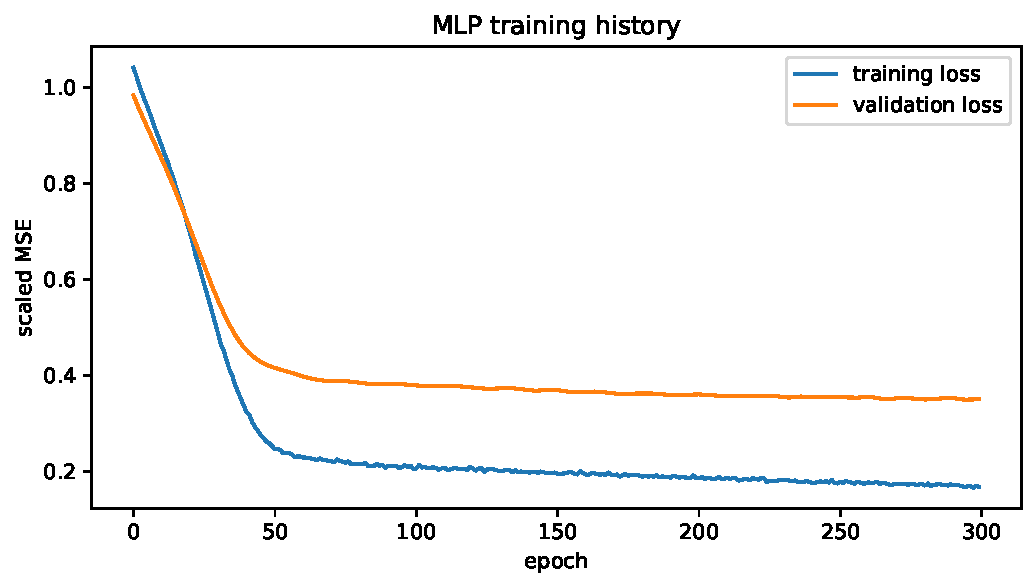
\includegraphics[keepaspectratio]{chapters/chapter-19-neural-networks-for-time-series_files/figure-pdf/ch19-pytorch-mlp-training-output-1.pdf}}

}

\caption{Training and validation loss curves for the window-based MLP.}

\end{figure}%

\section{19.14 Python example: evaluate the neural
forecast}\label{python-example-evaluate-the-neural-forecast}

We now evaluate on the held-out test period. The test set was not used
to fit preprocessing parameters, train the model, or choose the best
epoch.

\begin{Shaded}
\begin{Highlighting}[]
\NormalTok{model.}\BuiltInTok{eval}\NormalTok{()}
\ControlFlowTok{with}\NormalTok{ torch.no\_grad():}
\NormalTok{    mlp\_pred\_scaled }\OperatorTok{=}\NormalTok{ model(torch.tensor(Xs\_test, dtype}\OperatorTok{=}\NormalTok{torch.float32)).numpy()}

\NormalTok{mlp\_pred }\OperatorTok{=}\NormalTok{ y\_scaler.inverse\_transform(mlp\_pred\_scaled)}

\NormalTok{all\_results }\OperatorTok{=}\NormalTok{ baseline\_results }\OperatorTok{+}\NormalTok{ [}
\NormalTok{    forecast\_metrics(}\StringTok{"MLP window model"}\NormalTok{, Y\_test, mlp\_pred)}
\NormalTok{]}

\NormalTok{pd.DataFrame(all\_results).sort\_values(}\StringTok{"RMSE"}\NormalTok{)}
\end{Highlighting}
\end{Shaded}

\protect\phantomsection\label{ch19-mlp-test-evaluation}
{\def\LTcaptype{none} % do not increment counter
\begin{longtable}[]{@{}llll@{}}
\toprule\noalign{}
& model & RMSE & MAE \\
\midrule\noalign{}
\endhead
\bottomrule\noalign{}
\endlastfoot
1 & ridge window model & 0.499328 & 0.404376 \\
2 & MLP window model & 0.523898 & 0.425032 \\
0 & naive repeat-last & 1.236725 & 1.009598 \\
\end{longtable}
}

A neural model does not have to win every comparison. A strong linear
baseline may be difficult to beat when the data-generating mechanism is
mostly linear, the sample size is small, or the neural architecture is
not tuned. The correct conclusion is not always ``use a larger neural
network.'' The correct conclusion is to inspect the error by horizon,
validation design, and residual structure.

\begin{Shaded}
\begin{Highlighting}[]
\KeywordTok{def}\NormalTok{ rmse\_by\_horizon(truth, pred):}
    \ControlFlowTok{return}\NormalTok{ np.sqrt(np.mean((truth }\OperatorTok{{-}}\NormalTok{ pred) }\OperatorTok{**} \DecValTok{2}\NormalTok{, axis}\OperatorTok{=}\DecValTok{0}\NormalTok{))}

\NormalTok{horizons }\OperatorTok{=}\NormalTok{ np.arange(}\DecValTok{1}\NormalTok{, H }\OperatorTok{+} \DecValTok{1}\NormalTok{)}

\NormalTok{plt.figure(figsize}\OperatorTok{=}\NormalTok{(}\DecValTok{8}\NormalTok{, }\DecValTok{4}\NormalTok{))}
\NormalTok{plt.plot(horizons, rmse\_by\_horizon(Y\_test, naive\_pred), marker}\OperatorTok{=}\StringTok{"o"}\NormalTok{, label}\OperatorTok{=}\StringTok{"naive"}\NormalTok{)}
\NormalTok{plt.plot(horizons, rmse\_by\_horizon(Y\_test, ridge\_pred), marker}\OperatorTok{=}\StringTok{"o"}\NormalTok{, label}\OperatorTok{=}\StringTok{"ridge"}\NormalTok{)}
\NormalTok{plt.plot(horizons, rmse\_by\_horizon(Y\_test, mlp\_pred), marker}\OperatorTok{=}\StringTok{"o"}\NormalTok{, label}\OperatorTok{=}\StringTok{"MLP"}\NormalTok{)}
\NormalTok{plt.xlabel(}\StringTok{"forecast horizon"}\NormalTok{)}
\NormalTok{plt.ylabel(}\StringTok{"RMSE"}\NormalTok{)}
\NormalTok{plt.title(}\StringTok{"Horizon{-}wise forecast error"}\NormalTok{)}
\NormalTok{plt.legend()}
\NormalTok{plt.show()}
\end{Highlighting}
\end{Shaded}

\begin{figure}[H]

{\centering \pandocbounded{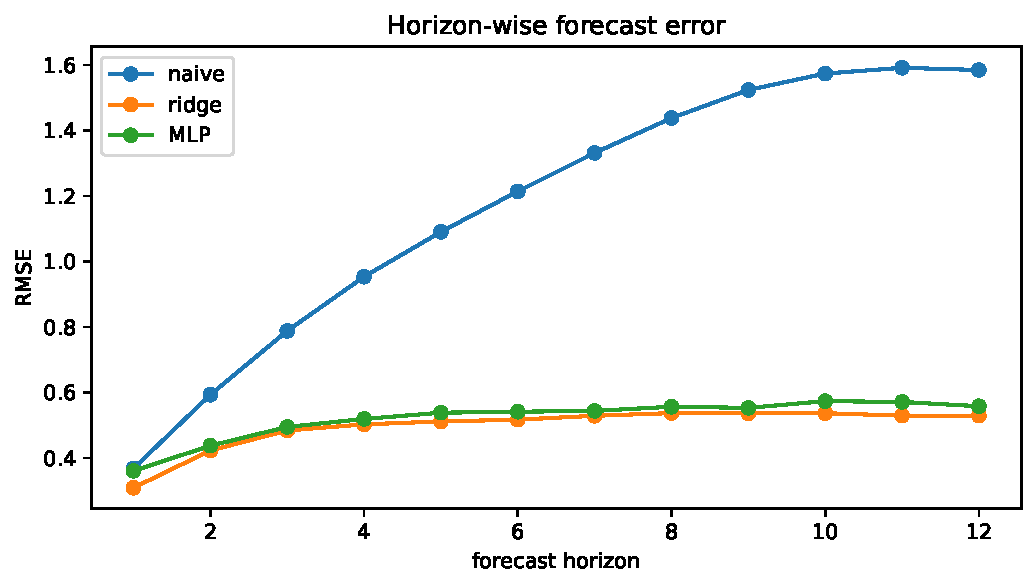
\includegraphics[keepaspectratio]{chapters/chapter-19-neural-networks-for-time-series_files/figure-pdf/ch19-horizon-errors-output-1.pdf}}

}

\caption{Forecast error by horizon for baseline, linear, and neural
models.}

\end{figure}%

\begin{Shaded}
\begin{Highlighting}[]
\NormalTok{case }\OperatorTok{=} \DecValTok{20}
\NormalTok{origin }\OperatorTok{=}\NormalTok{ origins[val\_end }\OperatorTok{+}\NormalTok{ case]}
\NormalTok{future\_index }\OperatorTok{=}\NormalTok{ np.arange(origin }\OperatorTok{+} \DecValTok{1}\NormalTok{, origin }\OperatorTok{+}\NormalTok{ H }\OperatorTok{+} \DecValTok{1}\NormalTok{)}
\NormalTok{history\_index }\OperatorTok{=}\NormalTok{ np.arange(origin }\OperatorTok{{-}}\NormalTok{ L }\OperatorTok{+} \DecValTok{1}\NormalTok{, origin }\OperatorTok{+} \DecValTok{1}\NormalTok{)}

\NormalTok{plt.figure(figsize}\OperatorTok{=}\NormalTok{(}\DecValTok{9}\NormalTok{, }\DecValTok{4}\NormalTok{))}
\NormalTok{plt.plot(history\_index, y[history\_index], label}\OperatorTok{=}\StringTok{"history"}\NormalTok{)}
\NormalTok{plt.plot(future\_index, Y\_test[case], marker}\OperatorTok{=}\StringTok{"o"}\NormalTok{, label}\OperatorTok{=}\StringTok{"future observed"}\NormalTok{)}
\NormalTok{plt.plot(future\_index, naive\_pred[case], marker}\OperatorTok{=}\StringTok{"o"}\NormalTok{, label}\OperatorTok{=}\StringTok{"naive"}\NormalTok{)}
\NormalTok{plt.plot(future\_index, ridge\_pred[case], marker}\OperatorTok{=}\StringTok{"o"}\NormalTok{, label}\OperatorTok{=}\StringTok{"ridge"}\NormalTok{)}
\NormalTok{plt.plot(future\_index, mlp\_pred[case], marker}\OperatorTok{=}\StringTok{"o"}\NormalTok{, label}\OperatorTok{=}\StringTok{"MLP"}\NormalTok{)}
\NormalTok{plt.axvline(origin, linestyle}\OperatorTok{=}\StringTok{"{-}{-}"}\NormalTok{, linewidth}\OperatorTok{=}\DecValTok{1}\NormalTok{)}
\NormalTok{plt.xlabel(}\StringTok{"time"}\NormalTok{)}
\NormalTok{plt.ylabel(}\StringTok{"value"}\NormalTok{)}
\NormalTok{plt.title(}\StringTok{"One multi{-}step forecast from a held{-}out test window"}\NormalTok{)}
\NormalTok{plt.legend()}
\NormalTok{plt.show()}
\end{Highlighting}
\end{Shaded}

\begin{figure}[H]

{\centering \pandocbounded{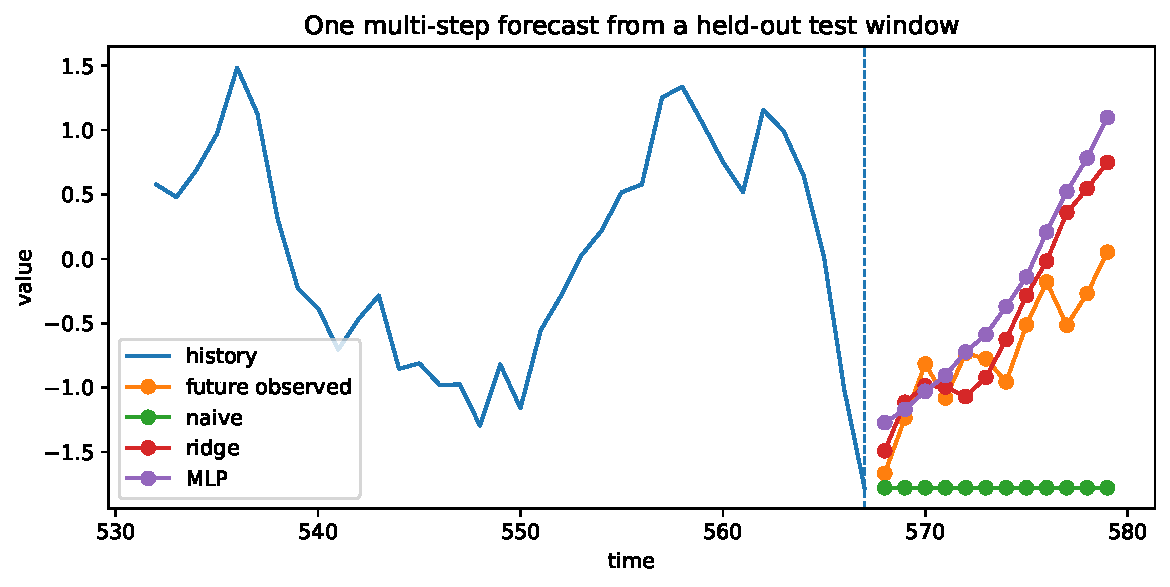
\includegraphics[keepaspectratio]{chapters/chapter-19-neural-networks-for-time-series_files/figure-pdf/ch19-forecast-path-example-output-1.pdf}}

}

\caption{One test-window forecast path from the MLP and benchmark
models.}

\end{figure}%

\section{19.15 Mini-batches and stochastic
optimization}\label{mini-batches-and-stochastic-optimization}

The code above used the full training set each epoch. Large neural
forecasting problems use mini-batches. If the training windows are

\[
\{(\mathbf x_i,\mathbf y_i):i=1,\ldots,N\},
\]

then a mini-batch \(B\subset\{1,\ldots,N\}\) gives the stochastic
gradient approximation

\[
\nabla_\theta J_B(\theta)
=
\frac{1}{|B|H}\sum_{i\in B}\sum_{h=1}^H
\nabla_\theta
\left(y_{i,h}-f_\theta(\mathbf x_i)_h\right)^2.
\]

The mini-batch examples can often be shuffled \textbf{within the
training period} because the model is trained on windows, not by
updating a hidden state through the original sequence. However, the
train-validation-test split itself should remain chronological.

\protect\phantomsection\label{ch19-dataloader-sketch}
\begin{Shaded}
\begin{Highlighting}[]
\ImportTok{from}\NormalTok{ torch.utils.data }\ImportTok{import}\NormalTok{ TensorDataset, DataLoader}

\NormalTok{train\_loader }\OperatorTok{=}\NormalTok{ DataLoader(}
\NormalTok{    TensorDataset(Xtr, Ytr),}
\NormalTok{    batch\_size}\OperatorTok{=}\DecValTok{64}\NormalTok{,}
\NormalTok{    shuffle}\OperatorTok{=}\VariableTok{True}\NormalTok{,}
\NormalTok{)}

\NormalTok{batch\_X, batch\_Y }\OperatorTok{=} \BuiltInTok{next}\NormalTok{(}\BuiltInTok{iter}\NormalTok{(train\_loader))}
\BuiltInTok{print}\NormalTok{(}\StringTok{"mini{-}batch X shape:"}\NormalTok{, }\BuiltInTok{tuple}\NormalTok{(batch\_X.shape))}
\BuiltInTok{print}\NormalTok{(}\StringTok{"mini{-}batch Y shape:"}\NormalTok{, }\BuiltInTok{tuple}\NormalTok{(batch\_Y.shape))}
\end{Highlighting}
\end{Shaded}

\begin{verbatim}
mini-batch X shape: (64, 36)
mini-batch Y shape: (64, 12)
\end{verbatim}

\section{19.16 Regularization and early
stopping}\label{regularization-and-early-stopping}

Neural time-series models can overfit badly because overlapping windows
create many similar training examples. Common regularization tools
include:

\begin{itemize}
\tightlist
\item
  small architectures;
\item
  weight decay;
\item
  dropout;
\item
  early stopping based on validation loss;
\item
  noise injection or data augmentation when justified;
\item
  limiting the input window length;
\item
  comparing against simple baselines.
\end{itemize}

Early stopping uses validation loss to choose a training epoch:

\[
\widehat k
=
\arg\min_k J_{\text{val}}(\theta_k).
\]

The test set should be used only once at the end.

\begin{tcolorbox}[enhanced jigsaw, arc=.35mm, bottomrule=.15mm, bottomtitle=1mm, breakable, colback=white, colbacktitle=quarto-callout-warning-color!10!white, colframe=quarto-callout-warning-color-frame, coltitle=black, left=2mm, leftrule=.75mm, opacityback=0, opacitybacktitle=0.6, rightrule=.15mm, title=\textcolor{quarto-callout-warning-color}{\faExclamationTriangle}\hspace{0.5em}{Many windows do not mean many independent examples}, titlerule=0mm, toprule=.15mm, toptitle=1mm]

If \(L=36\) and two adjacent training examples differ by only one time
step, the examples are highly overlapping. Neural networks may appear to
have a large training set, but the effective amount of independent
information may be much smaller.

\end{tcolorbox}

\section{19.17 Neural forecasting
workflow}\label{neural-forecasting-workflow}

A responsible neural forecasting workflow is:

\begin{enumerate}
\def\labelenumi{\arabic{enumi}.}
\tightlist
\item
  plot the data and build naive baselines;
\item
  define the forecast horizon and decision metric;
\item
  construct windows without using future information;
\item
  split chronologically into training, validation, and test periods;
\item
  fit scaling transformations on training data only;
\item
  train a small model first;
\item
  monitor training and validation losses;
\item
  compare against naive and linear baselines;
\item
  inspect horizon-wise errors;
\item
  write a diagnostic report describing where the model succeeds and
  fails.
\end{enumerate}

The model is only one part of the forecasting system. The validation
design often matters more than the architecture.

\section{19.18 AI-assisted modeling
activity}\label{ai-assisted-modeling-activity-2}

\section{AI-assisted study box}\label{ai-assisted-study-box}

Ask an AI assistant:

\begin{quote}
I am training a neural network to forecast a time series using sliding
windows. Give me a checklist of possible time leakage sources. For each
item, explain how I can test for it in code.
\end{quote}

Then verify the answer manually. In particular, check whether the
assistant remembers that scaling, feature construction, rolling
statistics, hyperparameter selection, and validation splits can all
introduce leakage.

\section{AI-assisted debugging
prompt}\label{ai-assisted-debugging-prompt}

Use the following prompt when your neural model performs too well:

\begin{quote}
My neural forecasting model has surprisingly low test error. Here is my
splitting code, scaling code, and feature construction code. Identify
any place where future information may enter the training process. Do
not suggest a new architecture until leakage has been ruled out.
\end{quote}

A suspiciously good forecast is often more dangerous than a bad
forecast.

\section{AI-assisted mathematical
explanation}\label{ai-assisted-mathematical-explanation}

Ask an AI assistant to explain why a linear neural network with no
nonlinear activations is equivalent to one linear layer. Then write the
proof yourself by composing two affine maps:

\[
W_2(W_1\mathbf x+\mathbf b_1)+\mathbf b_2
=
(W_2W_1)\mathbf x+(W_2\mathbf b_1+\mathbf b_2).
\]

\section{19.19 Common mistakes}\label{common-mistakes-18}

\begin{enumerate}
\def\labelenumi{\arabic{enumi}.}
\tightlist
\item
  \textbf{Using random train-test splits.} Random splits leak future
  regimes into the training set.
\item
  \textbf{Scaling before splitting.} The future test mean and variance
  should not be used during training.
\item
  \textbf{Skipping baselines.} A neural network that cannot beat a naive
  seasonal forecast is not useful.
\item
  \textbf{Confusing many windows with much information.} Overlapping
  windows are strongly dependent.
\item
  \textbf{Using too large a network.} Large networks can memorize local
  patterns in small time-series data sets.
\item
  \textbf{Evaluating only one-step forecasts.} Many applications require
  horizon-wise multi-step evaluation.
\item
  \textbf{Ignoring prediction uncertainty.} A point forecast alone may
  not support decision-making.
\item
  \textbf{Assuming deep learning removes feature thinking.} Calendar
  effects, known future covariates, and transformations often matter.
\end{enumerate}

\section{19.20 Exercises}\label{exercises-18}

\begin{enumerate}
\def\labelenumi{\arabic{enumi}.}
\tightlist
\item
  Let \(f_\theta:\mathbb R^L\to\mathbb R\) be a one-step neural
  forecast. Write the empirical MSE objective for forecast origins
  \(t=L,\ldots,T-1\).
\item
  Show that if every activation function is the identity, then a
  multilayer feedforward network represents an affine function.
\item
  For \(L=24\), \(H=6\), and \(T=500\), how many supervised windows can
  be constructed from a univariate series?
\item
  Explain why a random split of sliding windows may produce leakage even
  if no test target appears explicitly in the training set.
\item
  Modify the Python example so that \(H=1\). Compare the MLP with an
  AR-style ridge model.
\item
  Modify the Python example so that \(L=12,24,48\). Which input length
  gives the best validation loss?
\item
  Replace MSE loss with MAE or Huber loss. How do the forecasts change?
\item
  Add a known seasonal feature, such as \(\sin(2\pi t/24)\) and
  \(\cos(2\pi t/24)\), to the input. Compare performance.
\item
  Use recursive one-step forecasting instead of multi-output
  forecasting. Compare horizon-wise error curves.
\item
  Write a diagnostic report for the MLP model using a time plot, loss
  curve, horizon-wise RMSE, and one forecast-path example.
\end{enumerate}

\section{19.21 Mini project}\label{mini-project-2}

Choose one real time series and build a neural forecasting pipeline.

Your report should include:

\begin{enumerate}
\def\labelenumi{\arabic{enumi}.}
\tightlist
\item
  a clear forecasting question and horizon;
\item
  an exploratory plot and at least one seasonality or dependence
  diagnostic;
\item
  naive and linear baselines;
\item
  a window-based neural network;
\item
  chronological train-validation-test splitting;
\item
  scaling fit on the training period only;
\item
  horizon-wise error analysis;
\item
  a discussion of whether the neural network is justified;
\item
  an AI-assisted critique section where you ask an AI assistant to find
  weaknesses in your workflow and then verify or reject its suggestions.
\end{enumerate}

\section{19.22 Checklist}\label{checklist-3}

Before moving to CNNs, RNNs, LSTMs, and transformers, make sure you can
answer the following questions.

\begin{itemize}
\tightlist
\item
  What are \(L\) and \(H\) in a windowed forecasting problem?
\item
  What is the difference between sequence-to-one and
  sequence-to-sequence forecasting?
\item
  Why should time-series validation be chronological?
\item
  Why should scaling be fit on the training period only?
\item
  What baseline did your neural model beat?
\item
  Does your model's error increase with horizon?
\item
  Does the validation loss suggest overfitting?
\item
  Can you explain the model as a nonlinear autoregression?
\item
  Can you describe the loss function mathematically?
\item
  Can you identify at least three possible leakage sources?
\end{itemize}

\chapter{Convolutional Models for
Sequences}\label{convolutional-models-for-sequences}

\textbf{Part VI. Deep Learning for Time Series and Sequence Data}\\
\textbf{Chapter goal:} understand convolutional neural networks for
ordered data. We study one-dimensional convolution, causal convolution,
dilation, receptive fields, temporal convolutional networks,
multichannel sequence data, forecasting, classification, diagnostics,
and AI-assisted model critique.

\section{Learning objectives}\label{learning-objectives-19}

After studying this chapter, you should be able to:

\begin{enumerate}
\def\labelenumi{\arabic{enumi}.}
\tightlist
\item
  define a one-dimensional convolutional layer for univariate and
  multivariate sequences;
\item
  distinguish mathematical convolution from the cross-correlation
  operation used in most deep-learning libraries;
\item
  explain why causal padding is required for forecasting;
\item
  compute the receptive field of a stack of dilated convolutional
  layers;
\item
  compare convolutional sequence models with AR models, moving-average
  filters, and feedforward window models;
\item
  build a small temporal convolutional network in PyTorch;
\item
  evaluate convolutional forecasts using chronological validation and
  baselines;
\item
  identify leakage risks caused by padding, normalization, feature
  construction, and random windows;
\item
  use AI tools to inspect convolutional model code while verifying
  causality and validation design independently.
\end{enumerate}

\section{20.1 Motivation: local temporal
patterns}\label{motivation-local-temporal-patterns}

A sliding-window multilayer perceptron treats the input window

\[
(Y_{t-L+1},\ldots,Y_t)
\]

as a vector. This is useful, but it ignores a structural fact: nearby
time points are usually related. A sequence often contains local motifs
such as spikes, bursts, dips, oscillations, changes in slope, short
cycles, or repeated shapes. A convolutional model learns filters that
scan across time and detect such local patterns.

In image data, a two-dimensional convolution scans a small filter over a
grid. In sequence data, a one-dimensional convolution scans a small
filter over time. For a univariate sequence \(x_t\), a simple local
filter might compute

\[
z_t=w_0x_t+w_1x_{t-1}+w_2x_{t-2}.
\]

This resembles an autoregression or a moving-average filter. The
difference is that a convolutional neural network learns many filters,
applies nonlinear activations, stacks layers, and can learn nonlinear
temporal features.

\begin{tcolorbox}[enhanced jigsaw, arc=.35mm, bottomrule=.15mm, bottomtitle=1mm, breakable, colback=white, colbacktitle=quarto-callout-note-color!10!white, colframe=quarto-callout-note-color-frame, coltitle=black, left=2mm, leftrule=.75mm, opacityback=0, opacitybacktitle=0.6, rightrule=.15mm, title=\textcolor{quarto-callout-note-color}{\faInfo}\hspace{0.5em}{Convolutions connect classical and modern sequence modeling}, titlerule=0mm, toprule=.15mm, toptitle=1mm]

A linear causal convolution is a finite impulse-response filter. A
temporal convolutional network is a nonlinear composition of many such
filters. This makes CNNs a natural bridge between classical time-series
filtering and modern deep learning.

\end{tcolorbox}

\section{20.2 One-dimensional
convolution}\label{one-dimensional-convolution}

Let \(x=(x_1,\ldots,x_T)\) be a univariate sequence. A length-\(K\)
filter has weights

\[
\mathbf w=(w_0,w_1,\ldots,w_{K-1}).
\]

A \textbf{causal} one-dimensional convolution with dilation \(d\ge 1\)
is

\[
z_t=b+\sum_{j=0}^{K-1} w_j x_{t-dj}.
\]

The value \(z_t\) depends only on \(x_t,x_{t-d},x_{t-2d},\ldots\). It
does not depend on future values \(x_{t+1},x_{t+2},\ldots\). This is
essential for forecasting.

For indices \(t-dj<1\), we must decide how to handle the missing past.
Common choices are:

\begin{itemize}
\tightlist
\item
  left zero padding;
\item
  left replication padding;
\item
  dropping early output times;
\item
  using an initial history from before the forecast period.
\end{itemize}

In forecasting, padding must not introduce information from the future.

\subsection{Cross-correlation versus mathematical
convolution}\label{cross-correlation-versus-mathematical-convolution}

Many deep-learning libraries call the following operation convolution:

\[
z_t=b+\sum_{j=0}^{K-1} w_j x_{t+j}.
\]

Mathematically, this is closer to \textbf{cross-correlation}, because
the filter is not reversed. In deep learning, this distinction is
usually harmless because the filter weights are learned. For
forecasting, the important issue is not whether the kernel is reversed;
the important issue is whether the output uses future inputs.

A safe causal forecasting layer should satisfy

\[
\widehat Y_{t+h}\text{ computed at forecast origin }t
\quad\text{cannot depend on}\quad
Y_{t+1},Y_{t+2},\ldots.
\]

\section{20.3 Multichannel sequence
convolution}\label{multichannel-sequence-convolution}

Many sequence problems are multivariate. Suppose

\[
\mathbf x_t=(x_{t,1},\ldots,x_{t,C})\in\mathbb R^C
\]

has \(C\) input channels. A convolutional layer with \(M\) output
channels has filters

\[
W_{m,c,j},
\qquad
m=1,\ldots,M,
\quad c=1,\ldots,C,
\quad j=0,\ldots,K-1.
\]

The \(m\)-th output channel is

\[
z_{t,m}=b_m+
\sum_{c=1}^C\sum_{j=0}^{K-1} W_{m,c,j}x_{t-dj,c}.
\]

The tensor of weights has shape

\[
M\times C\times K.
\]

A nonlinear activation, such as ReLU or GELU, is then applied:

\[
h_{t,m}=\sigma(z_{t,m}).
\]

This creates learned temporal features. Different output channels can
learn different detectors: a rising-edge detector, a falling-edge
detector, a short-cycle detector, a spike detector, or an interaction
between variables.

\section{20.4 Stride, padding, and
dilation}\label{stride-padding-and-dilation}

Three parameters control the geometry of a convolutional layer.

\subsection{Kernel size}\label{kernel-size}

The kernel size \(K\) is the number of time points used by one filter.
Larger \(K\) allows each layer to inspect a wider local pattern.

\subsection{Stride}\label{stride}

Stride \(s\) controls how far the filter moves between output positions.
A stride of \(s=1\) gives one output at each time. A stride larger than
\(1\) downsamples the sequence. For forecasting, stride \(1\) is common
inside the model; downsampling may be useful in encoder architectures.

\subsection{Dilation}\label{dilation}

Dilation \(d\) spaces out the filter taps:

\[
z_t=b+w_0x_t+w_1x_{t-d}+w_2x_{t-2d}+\cdots+w_{K-1}x_{t-(K-1)d}.
\]

Dilation lets the model reach further into the past without increasing
the number of parameters. This is the key idea behind many temporal
convolutional networks.

\begin{tcolorbox}[enhanced jigsaw, arc=.35mm, bottomrule=.15mm, bottomtitle=1mm, breakable, colback=white, colbacktitle=quarto-callout-tip-color!10!white, colframe=quarto-callout-tip-color-frame, coltitle=black, left=2mm, leftrule=.75mm, opacityback=0, opacitybacktitle=0.6, rightrule=.15mm, title=\textcolor{quarto-callout-tip-color}{\faLightbulb}\hspace{0.5em}{Why dilation matters}, titlerule=0mm, toprule=.15mm, toptitle=1mm]

With \(K=3\) and \(d=1\), a layer uses \(x_t,x_{t-1},x_{t-2}\). With
\(K=3\) and \(d=8\), a layer uses \(x_t,x_{t-8},x_{t-16}\). The number
of weights is still only three, but the temporal reach is much larger.

\end{tcolorbox}

\section{20.5 Interactive module: causal dilated
convolution}\label{interactive-module-causal-dilated-convolution}

The interactive module below shows a causal dilated convolution. The
selected output time \(t_0\) depends on the input values

\[
x_{t_0},x_{t_0-d},x_{t_0-2d},\ldots,x_{t_0-(K-1)d}.
\]

Move the sliders and check that the highlighted input points never occur
after \(t_0\).

Interactive Module 20A: Causal Dilated Convolution

The output at the selected time uses only the present and past input
values.

\begin{verbatim}
<label>
  Kernel size $K$:
  <input id="ch20_kernel" type="range" min="2" max="7" step="1" value="3">
  <span id="ch20_kernel_value">3</span>
</label>

<label>
  Dilation $d$:
  <input id="ch20_dilation" type="range" min="1" max="10" step="1" value="2">
  <span id="ch20_dilation_value">2</span>
</label>

<label>
  Output time $t_0$:
  <input id="ch20_time" type="range" min="0" max="95" step="1" value="45">
  <span id="ch20_time_value">45</span>
</label>
\end{verbatim}

\protect\phantomsection\label{ch20_conv_plot}

\section{20.6 Receptive fields}\label{receptive-fields}

The \textbf{receptive field} of an output is the set of input times that
can influence that output.

For one causal dilated convolutional layer with kernel size \(K\) and
dilation \(d\), the output \(z_t\) depends on

\[
t,
\quad t-d,
\quad t-2d,
\quad \ldots,
\quad t-(K-1)d.
\]

The temporal width of this receptive field is

\[
R=1+(K-1)d.
\]

For a stack of \(L\) causal convolutional layers with stride \(1\),
kernel size \(K\), and dilations \(d_1,\ldots,d_L\), the receptive-field
width is

\[
R_L=1+(K-1)\sum_{\ell=1}^L d_\ell.
\]

\subsection{Proof idea}\label{proof-idea-1}

The first layer can move backward by at most \((K-1)d_1\) time steps.
The second layer can move backward by an additional \((K-1)d_2\) time
steps relative to the first-layer features. Continuing through \(L\)
layers gives the maximum backward reach

\[
(K-1)d_1+\cdots+(K-1)d_L.
\]

Including the current time itself gives

\[
R_L=1+(K-1)\sum_{\ell=1}^L d_\ell.
\]

If the dilations double,

\[
d_\ell=2^{\ell-1},
\]

then

\[
R_L=1+(K-1)(2^L-1).
\]

This exponential growth is why dilated CNNs can model long histories
efficiently.

\section{20.7 Interactive module: receptive-field
growth}\label{interactive-module-receptive-field-growth}

The next module shows which relative lags can affect the final output at
time \(t\). A marker at relative lag \(-12\) means that \(x_{t-12}\) can
influence the output.

Interactive Module 20B: Receptive Field of a TCN Stack

\begin{verbatim}
<label>
  Layers $L$:
  <input id="ch20_layers" type="range" min="1" max="7" step="1" value="4">
  <span id="ch20_layers_value">4</span>
</label>

<label>
  Kernel size $K$:
  <input id="ch20_rf_kernel" type="range" min="2" max="6" step="1" value="3">
  <span id="ch20_rf_kernel_value">3</span>
</label>

<label>
  Constant dilation:
  <input id="ch20_rf_dilation" type="range" min="1" max="8" step="1" value="2">
  <span id="ch20_rf_dilation_value">2</span>
</label>

<label>
  Dilation schedule:
  <select id="ch20_rf_mode">
    <option value="exp" selected>powers of two: 1, 2, 4, ...</option>
    <option value="constant">constant dilation</option>
  </select>
</label>
\end{verbatim}

\protect\phantomsection\label{ch20_rf_plot}

\section{20.8 Temporal convolutional
networks}\label{temporal-convolutional-networks}

A \textbf{temporal convolutional network} or \textbf{TCN} is a neural
architecture built from causal one-dimensional convolutional layers. A
common TCN block has the form

\[
\mathbf H^{(\ell)}
=
\mathbf H^{(\ell-1)}+F_\ell(\mathbf H^{(\ell-1)}),
\]

where \(F_\ell\) contains causal dilated convolutions, nonlinearities,
normalization, and dropout. The addition is a residual connection.

A simplified block is

\[
F_\ell(\mathbf H)
=\operatorname{Dropout}
\left(
\sigma\left(\operatorname{Conv}_{K,d_\ell}(\mathbf H)\right)
\right).
\]

Residual connections help optimization by giving gradients a direct path
through the network. Dilations give the block a long memory. Dropout and
weight decay help reduce overfitting.

A TCN is usually:

\begin{itemize}
\tightlist
\item
  \textbf{causal}, so no future values enter the forecast;
\item
  \textbf{convolutional}, so the same filter weights are reused across
  time;
\item
  \textbf{dilated}, so the receptive field grows quickly;
\item
  \textbf{residual}, so deep stacks are easier to train.
\end{itemize}

\section{20.9 CNNs versus AR models and
filters}\label{cnns-versus-ar-models-and-filters}

A causal linear convolution

\[
z_t=\sum_{j=0}^{K-1}w_jx_{t-j}
\]

is mathematically similar to a finite-order autoregressive predictor or
a finite impulse-response filter. However, a CNN differs in several
ways.

First, a CNN uses many filters. Instead of one scalar output, it creates
feature channels:

\[
h_{t,1},h_{t,2},\ldots,h_{t,M}.
\]

Second, nonlinear activations make the model nonlinear:

\[
h_{t,m}=\sigma\left(b_m+\sum_{j=0}^{K-1}w_{m,j}x_{t-j}\right).
\]

Third, stacking layers creates hierarchical temporal features. A first
layer may detect short-term rises and drops; later layers may combine
these into longer patterns.

Fourth, dilation lets the model use sparse long-range lags without the
dense parameter count of a large fully connected window.

\begin{tcolorbox}[enhanced jigsaw, arc=.35mm, bottomrule=.15mm, bottomtitle=1mm, breakable, colback=white, colbacktitle=quarto-callout-note-color!10!white, colframe=quarto-callout-note-color-frame, coltitle=black, left=2mm, leftrule=.75mm, opacityback=0, opacitybacktitle=0.6, rightrule=.15mm, title=\textcolor{quarto-callout-note-color}{\faInfo}\hspace{0.5em}{Linear special case}, titlerule=0mm, toprule=.15mm, toptitle=1mm]

If all activations are the identity and there is only one output
channel, a convolutional network collapses to a linear time-invariant
filter. The nonlinear power of CNNs comes from multiple channels,
nonlinear activations, and layer composition.

\end{tcolorbox}

\section{20.10 Forecasting with convolutional
models}\label{forecasting-with-convolutional-models}

For forecasting, a convolutional model usually maps an input window to
one or more future values:

\[
f_\theta:\mathbb R^{L\times C}\to\mathbb R^H.
\]

For a training set of forecast origins \(t\), the empirical risk is

\[
J(\theta)=
\frac{1}{N}\sum_{t\in\mathcal T_{\text{train}}}
\ell\left(
\widehat{\mathbf y}_t,
\mathbf y_t
\right),
\]

where

\[
\widehat{\mathbf y}_t=f_\theta(\mathbf X_t),
\qquad
\mathbf y_t=(Y_{t+1},\ldots,Y_{t+H}).
\]

For mean squared error,

\[
\ell(\widehat{\mathbf y}_t,\mathbf y_t)
=
\frac{1}{H}\sum_{h=1}^H
(\widehat Y_{t+h|t}-Y_{t+h})^2.
\]

For probabilistic forecasting, the output layer can produce quantiles,
distribution parameters, or simulation paths. For example, a quantile
CNN can minimize pinball loss for several quantile levels.

\section{20.11 Python example: convolution from
scratch}\label{python-example-convolution-from-scratch}

The following code implements a causal dilated convolution directly.
This makes the indexing visible.

\begin{Shaded}
\begin{Highlighting}[]
\ImportTok{import}\NormalTok{ numpy }\ImportTok{as}\NormalTok{ np}
\ImportTok{import}\NormalTok{ matplotlib.pyplot }\ImportTok{as}\NormalTok{ plt}

\NormalTok{np.random.seed(}\DecValTok{7339}\NormalTok{)}

\NormalTok{T }\OperatorTok{=} \DecValTok{96}
\NormalTok{t }\OperatorTok{=}\NormalTok{ np.arange(T)}
\NormalTok{x }\OperatorTok{=}\NormalTok{ (}
\NormalTok{    np.sin(}\DecValTok{2} \OperatorTok{*}\NormalTok{ np.pi }\OperatorTok{*}\NormalTok{ t }\OperatorTok{/} \DecValTok{24}\NormalTok{)}
    \OperatorTok{+} \FloatTok{0.35} \OperatorTok{*}\NormalTok{ np.sin(}\DecValTok{2} \OperatorTok{*}\NormalTok{ np.pi }\OperatorTok{*}\NormalTok{ t }\OperatorTok{/} \DecValTok{6}\NormalTok{)}
    \OperatorTok{+} \FloatTok{0.03} \OperatorTok{*}\NormalTok{ t}
\NormalTok{)}

\NormalTok{kernel }\OperatorTok{=}\NormalTok{ np.array([}\FloatTok{0.60}\NormalTok{, }\FloatTok{0.30}\NormalTok{, }\OperatorTok{{-}}\FloatTok{0.25}\NormalTok{])}
\NormalTok{dilation }\OperatorTok{=} \DecValTok{4}

\KeywordTok{def}\NormalTok{ causal\_dilated\_conv\_1d(x, kernel, dilation}\OperatorTok{=}\DecValTok{1}\NormalTok{):}
    \CommentTok{"""Causal dilated convolution with left zero padding."""}
\NormalTok{    T }\OperatorTok{=} \BuiltInTok{len}\NormalTok{(x)}
\NormalTok{    K }\OperatorTok{=} \BuiltInTok{len}\NormalTok{(kernel)}
\NormalTok{    y }\OperatorTok{=}\NormalTok{ np.zeros(T)}
    \ControlFlowTok{for}\NormalTok{ time }\KeywordTok{in} \BuiltInTok{range}\NormalTok{(T):}
\NormalTok{        total }\OperatorTok{=} \FloatTok{0.0}
        \ControlFlowTok{for}\NormalTok{ j }\KeywordTok{in} \BuiltInTok{range}\NormalTok{(K):}
\NormalTok{            idx }\OperatorTok{=}\NormalTok{ time }\OperatorTok{{-}}\NormalTok{ dilation }\OperatorTok{*}\NormalTok{ j}
            \ControlFlowTok{if}\NormalTok{ idx }\OperatorTok{\textgreater{}=} \DecValTok{0}\NormalTok{:}
\NormalTok{                total }\OperatorTok{+=}\NormalTok{ kernel[j] }\OperatorTok{*}\NormalTok{ x[idx]}
\NormalTok{        y[time] }\OperatorTok{=}\NormalTok{ total}
    \ControlFlowTok{return}\NormalTok{ y}

\NormalTok{y }\OperatorTok{=}\NormalTok{ causal\_dilated\_conv\_1d(x, kernel, dilation}\OperatorTok{=}\NormalTok{dilation)}

\NormalTok{plt.figure(figsize}\OperatorTok{=}\NormalTok{(}\DecValTok{10}\NormalTok{, }\DecValTok{4}\NormalTok{))}
\NormalTok{plt.plot(t, x, label}\OperatorTok{=}\StringTok{"input sequence"}\NormalTok{)}
\NormalTok{plt.plot(t, y, label}\OperatorTok{=}\StringTok{"causal dilated convolution"}\NormalTok{)}
\NormalTok{plt.xlabel(}\StringTok{"time"}\NormalTok{)}
\NormalTok{plt.ylabel(}\StringTok{"value"}\NormalTok{)}
\NormalTok{plt.title(}\StringTok{"Causal dilated convolution from scratch"}\NormalTok{)}
\NormalTok{plt.legend()}
\NormalTok{plt.show()}
\end{Highlighting}
\end{Shaded}

\begin{figure}[H]

{\centering \pandocbounded{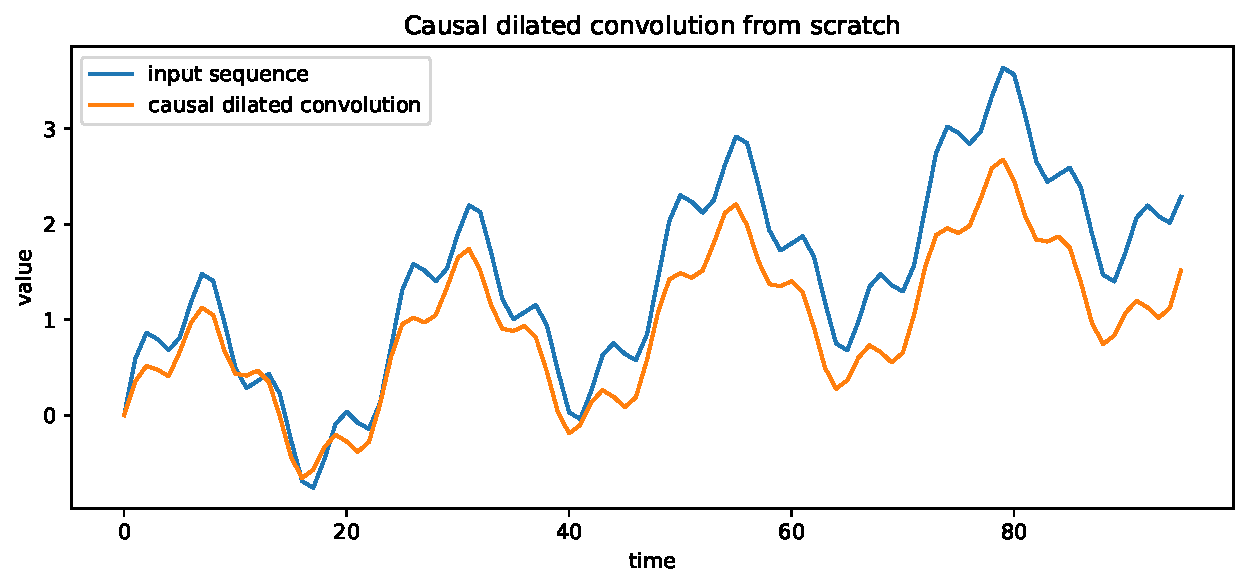
\includegraphics[keepaspectratio]{chapters/chapter-20-convolutional-models-sequences_files/figure-pdf/ch20-causal-convolution-from-scratch-output-1.pdf}}

}

\caption{A causal dilated convolution uses only current and past
inputs.}

\end{figure}%

The output \(y_t\) is a filtered version of the input. Because the
filter is causal, the value at time \(t\) does not use \(x_{t+1}\) or
any later value.

\section{\texorpdfstring{20.12 Python example: checking PyTorch
\texttt{Conv1d}}{20.12 Python example: checking PyTorch Conv1d}}\label{python-example-checking-pytorch-conv1d}

PyTorch uses tensors with shape

\[
\text{batch}\times\text{channels}\times\text{time}.
\]

The module \texttt{nn.Conv1d} does not automatically implement left-only
causal padding. A common safe pattern is:

\begin{enumerate}
\def\labelenumi{\arabic{enumi}.}
\tightlist
\item
  add left padding manually;
\item
  use \texttt{Conv1d} with \texttt{padding=0};
\item
  verify output length and causality.
\end{enumerate}

\protect\phantomsection\label{ch20-pytorch-causal-conv}
\begin{Shaded}
\begin{Highlighting}[]
\ImportTok{import}\NormalTok{ torch}
\ImportTok{from}\NormalTok{ torch }\ImportTok{import}\NormalTok{ nn}
\NormalTok{torch.set\_num\_threads(}\DecValTok{1}\NormalTok{)}

\KeywordTok{class}\NormalTok{ CausalConv1d(nn.Module):}
    \KeywordTok{def} \FunctionTok{\_\_init\_\_}\NormalTok{(}\VariableTok{self}\NormalTok{, in\_channels, out\_channels, kernel\_size, dilation}\OperatorTok{=}\DecValTok{1}\NormalTok{):}
        \BuiltInTok{super}\NormalTok{().}\FunctionTok{\_\_init\_\_}\NormalTok{()}
        \VariableTok{self}\NormalTok{.left\_padding }\OperatorTok{=}\NormalTok{ dilation }\OperatorTok{*}\NormalTok{ (kernel\_size }\OperatorTok{{-}} \DecValTok{1}\NormalTok{)}
        \VariableTok{self}\NormalTok{.conv }\OperatorTok{=}\NormalTok{ nn.Conv1d(}
\NormalTok{            in\_channels}\OperatorTok{=}\NormalTok{in\_channels,}
\NormalTok{            out\_channels}\OperatorTok{=}\NormalTok{out\_channels,}
\NormalTok{            kernel\_size}\OperatorTok{=}\NormalTok{kernel\_size,}
\NormalTok{            dilation}\OperatorTok{=}\NormalTok{dilation,}
\NormalTok{            padding}\OperatorTok{=}\DecValTok{0}\NormalTok{,}
\NormalTok{            bias}\OperatorTok{=}\VariableTok{False}\NormalTok{,}
\NormalTok{        )}

    \KeywordTok{def}\NormalTok{ forward(}\VariableTok{self}\NormalTok{, x):}
        \CommentTok{\# x shape: batch, channels, time}
\NormalTok{        x\_pad }\OperatorTok{=}\NormalTok{ nn.functional.pad(x, (}\VariableTok{self}\NormalTok{.left\_padding, }\DecValTok{0}\NormalTok{))}
        \ControlFlowTok{return} \VariableTok{self}\NormalTok{.conv(x\_pad)}

\CommentTok{\# Build a one{-}filter layer and set weights equal to the NumPy kernel.}
\NormalTok{torch.manual\_seed(}\DecValTok{7339}\NormalTok{)}
\NormalTok{layer }\OperatorTok{=}\NormalTok{ CausalConv1d(}\DecValTok{1}\NormalTok{, }\DecValTok{1}\NormalTok{, kernel\_size}\OperatorTok{=}\DecValTok{3}\NormalTok{, dilation}\OperatorTok{=}\NormalTok{dilation)}
\ControlFlowTok{with}\NormalTok{ torch.no\_grad():}
    \CommentTok{\# PyTorch Conv1d applies cross{-}correlation, so reverse the weights}
    \CommentTok{\# to match the causal formula y\_t = sum\_j kernel[j] x\_\{t{-}dj\}.}
\NormalTok{    layer.conv.weight[:] }\OperatorTok{=}\NormalTok{ torch.tensor(kernel[::}\OperatorTok{{-}}\DecValTok{1}\NormalTok{].copy().reshape(}\DecValTok{1}\NormalTok{, }\DecValTok{1}\NormalTok{, }\OperatorTok{{-}}\DecValTok{1}\NormalTok{), dtype}\OperatorTok{=}\NormalTok{torch.float32)}

\NormalTok{x\_tensor }\OperatorTok{=}\NormalTok{ torch.tensor(x.reshape(}\DecValTok{1}\NormalTok{, }\DecValTok{1}\NormalTok{, }\OperatorTok{{-}}\DecValTok{1}\NormalTok{), dtype}\OperatorTok{=}\NormalTok{torch.float32)}
\NormalTok{y\_torch }\OperatorTok{=}\NormalTok{ layer(x\_tensor).detach().numpy().reshape(}\OperatorTok{{-}}\DecValTok{1}\NormalTok{)}

\BuiltInTok{print}\NormalTok{(}\StringTok{"Output length:"}\NormalTok{, }\BuiltInTok{len}\NormalTok{(y\_torch))}
\BuiltInTok{print}\NormalTok{(}\StringTok{"Maximum absolute difference from NumPy:"}\NormalTok{, np.}\BuiltInTok{max}\NormalTok{(np.}\BuiltInTok{abs}\NormalTok{(y\_torch }\OperatorTok{{-}}\NormalTok{ y)))}
\end{Highlighting}
\end{Shaded}

\begin{verbatim}
Output length: 96
Maximum absolute difference from NumPy: 2.0040756965045148e-07
\end{verbatim}

This direct comparison is a good habit. Before building a large
architecture, verify that the low-level sequence geometry is correct.

\section{20.13 Causality test for a neural
layer}\label{causality-test-for-a-neural-layer}

A practical way to test causality is to perturb future values and check
whether earlier outputs change. Suppose we compare two inputs that agree
up to time \(t\) and differ after time \(t\). A causal model should
produce identical outputs up to time \(t\).

\protect\phantomsection\label{ch20-causality-test}
\begin{Shaded}
\begin{Highlighting}[]
\NormalTok{x1 }\OperatorTok{=}\NormalTok{ torch.tensor(x.reshape(}\DecValTok{1}\NormalTok{, }\DecValTok{1}\NormalTok{, }\OperatorTok{{-}}\DecValTok{1}\NormalTok{), dtype}\OperatorTok{=}\NormalTok{torch.float32)}
\NormalTok{x2 }\OperatorTok{=}\NormalTok{ x1.clone()}
\NormalTok{x2[:, :, }\DecValTok{60}\NormalTok{:] }\OperatorTok{=}\NormalTok{ x2[:, :, }\DecValTok{60}\NormalTok{:] }\OperatorTok{+} \FloatTok{1000.0}  \CommentTok{\# huge future perturbation}

\ControlFlowTok{with}\NormalTok{ torch.no\_grad():}
\NormalTok{    y1 }\OperatorTok{=}\NormalTok{ layer(x1)}
\NormalTok{    y2 }\OperatorTok{=}\NormalTok{ layer(x2)}

\NormalTok{max\_change\_before\_60 }\OperatorTok{=}\NormalTok{ (y1[:, :, :}\DecValTok{60}\NormalTok{] }\OperatorTok{{-}}\NormalTok{ y2[:, :, :}\DecValTok{60}\NormalTok{]).}\BuiltInTok{abs}\NormalTok{().}\BuiltInTok{max}\NormalTok{().item()}
\NormalTok{max\_change\_after\_60 }\OperatorTok{=}\NormalTok{ (y1[:, :, }\DecValTok{60}\NormalTok{:] }\OperatorTok{{-}}\NormalTok{ y2[:, :, }\DecValTok{60}\NormalTok{:]).}\BuiltInTok{abs}\NormalTok{().}\BuiltInTok{max}\NormalTok{().item()}

\BuiltInTok{print}\NormalTok{(}\StringTok{"Max output change before time 60:"}\NormalTok{, max\_change\_before\_60)}
\BuiltInTok{print}\NormalTok{(}\StringTok{"Max output change from time 60 onward:"}\NormalTok{, max\_change\_after\_60)}
\end{Highlighting}
\end{Shaded}

\begin{verbatim}
Max output change before time 60: 0.0
Max output change from time 60 onward: 900.0000610351562
\end{verbatim}

If the first number is not approximately zero, the layer is leaking
future information.

\section{20.14 Building windows for CNN
forecasting}\label{building-windows-for-cnn-forecasting}

A CNN input window for a univariate series has shape

\[
1\times L,
\]

where the first dimension is the channel dimension. For a multivariate
series with \(C\) variables, the input has shape

\[
C\times L.
\]

A batch of \(B\) examples has shape

\[
B\times C\times L.
\]

The target for a multi-step forecast has shape

\[
B\times H.
\]

The next example builds a synthetic data set and converts it into CNN
windows.

\protect\phantomsection\label{ch20-window-dataset}
\begin{Shaded}
\begin{Highlighting}[]
\ImportTok{from}\NormalTok{ torch.utils.data }\ImportTok{import}\NormalTok{ Dataset, DataLoader}

\NormalTok{np.random.seed(}\DecValTok{7339}\NormalTok{)}
\NormalTok{T }\OperatorTok{=} \DecValTok{520}
\NormalTok{t }\OperatorTok{=}\NormalTok{ np.arange(T)}
\NormalTok{y\_series }\OperatorTok{=}\NormalTok{ (}
    \FloatTok{0.003} \OperatorTok{*}\NormalTok{ t}
    \OperatorTok{+}\NormalTok{ np.sin(}\DecValTok{2} \OperatorTok{*}\NormalTok{ np.pi }\OperatorTok{*}\NormalTok{ t }\OperatorTok{/} \DecValTok{24}\NormalTok{)}
    \OperatorTok{+} \FloatTok{0.45} \OperatorTok{*}\NormalTok{ np.sin(}\DecValTok{2} \OperatorTok{*}\NormalTok{ np.pi }\OperatorTok{*}\NormalTok{ t }\OperatorTok{/} \DecValTok{7}\NormalTok{)}
    \OperatorTok{+} \FloatTok{0.25} \OperatorTok{*}\NormalTok{ np.random.randn(T)}
\NormalTok{)}

\NormalTok{L }\OperatorTok{=} \DecValTok{48}
\NormalTok{H }\OperatorTok{=} \DecValTok{6}

\KeywordTok{class}\NormalTok{ WindowDataset(Dataset):}
    \KeywordTok{def} \FunctionTok{\_\_init\_\_}\NormalTok{(}\VariableTok{self}\NormalTok{, values, input\_length, horizon):}
        \VariableTok{self}\NormalTok{.values }\OperatorTok{=}\NormalTok{ np.asarray(values, dtype}\OperatorTok{=}\NormalTok{np.float32)}
        \VariableTok{self}\NormalTok{.input\_length }\OperatorTok{=}\NormalTok{ input\_length}
        \VariableTok{self}\NormalTok{.horizon }\OperatorTok{=}\NormalTok{ horizon}

    \KeywordTok{def} \FunctionTok{\_\_len\_\_}\NormalTok{(}\VariableTok{self}\NormalTok{):}
        \ControlFlowTok{return} \BuiltInTok{len}\NormalTok{(}\VariableTok{self}\NormalTok{.values) }\OperatorTok{{-}} \VariableTok{self}\NormalTok{.input\_length }\OperatorTok{{-}} \VariableTok{self}\NormalTok{.horizon }\OperatorTok{+} \DecValTok{1}

    \KeywordTok{def} \FunctionTok{\_\_getitem\_\_}\NormalTok{(}\VariableTok{self}\NormalTok{, idx):}
\NormalTok{        x\_window }\OperatorTok{=} \VariableTok{self}\NormalTok{.values[idx:idx }\OperatorTok{+} \VariableTok{self}\NormalTok{.input\_length]}
\NormalTok{        y\_window }\OperatorTok{=} \VariableTok{self}\NormalTok{.values[idx }\OperatorTok{+} \VariableTok{self}\NormalTok{.input\_length:idx }\OperatorTok{+} \VariableTok{self}\NormalTok{.input\_length }\OperatorTok{+} \VariableTok{self}\NormalTok{.horizon]}
        \CommentTok{\# Conv1d expects channels before time.}
\NormalTok{        x\_window }\OperatorTok{=}\NormalTok{ x\_window.reshape(}\DecValTok{1}\NormalTok{, }\OperatorTok{{-}}\DecValTok{1}\NormalTok{)}
        \ControlFlowTok{return}\NormalTok{ torch.tensor(x\_window), torch.tensor(y\_window)}

\CommentTok{\# Chronological split before scaling.}
\NormalTok{train\_end }\OperatorTok{=} \DecValTok{360}
\NormalTok{val\_end }\OperatorTok{=} \DecValTok{440}

\NormalTok{train\_values }\OperatorTok{=}\NormalTok{ y\_series[:train\_end]}
\NormalTok{train\_mean }\OperatorTok{=}\NormalTok{ train\_values.mean()}
\NormalTok{train\_std }\OperatorTok{=}\NormalTok{ train\_values.std()}

\NormalTok{y\_scaled }\OperatorTok{=}\NormalTok{ (y\_series }\OperatorTok{{-}}\NormalTok{ train\_mean) }\OperatorTok{/}\NormalTok{ train\_std}

\NormalTok{train\_ds }\OperatorTok{=}\NormalTok{ WindowDataset(y\_scaled[:train\_end], L, H)}
\NormalTok{val\_ds }\OperatorTok{=}\NormalTok{ WindowDataset(y\_scaled[train\_end }\OperatorTok{{-}}\NormalTok{ L:val\_end], L, H)}
\NormalTok{test\_ds }\OperatorTok{=}\NormalTok{ WindowDataset(y\_scaled[val\_end }\OperatorTok{{-}}\NormalTok{ L:], L, H)}

\NormalTok{x\_batch, y\_batch }\OperatorTok{=}\NormalTok{ train\_ds[}\DecValTok{0}\NormalTok{]}
\BuiltInTok{print}\NormalTok{(}\StringTok{"One input shape:"}\NormalTok{, }\BuiltInTok{tuple}\NormalTok{(x\_batch.shape))}
\BuiltInTok{print}\NormalTok{(}\StringTok{"One target shape:"}\NormalTok{, }\BuiltInTok{tuple}\NormalTok{(y\_batch.shape))}
\BuiltInTok{print}\NormalTok{(}\StringTok{"Number of training windows:"}\NormalTok{, }\BuiltInTok{len}\NormalTok{(train\_ds))}
\end{Highlighting}
\end{Shaded}

\begin{verbatim}
One input shape: (1, 48)
One target shape: (6,)
Number of training windows: 307
\end{verbatim}

The validation and test segments include \(L\) previous observations so
that the first validation/test windows have enough history. The mean and
standard deviation are still computed only from the training period.

\section{20.15 A small TCN forecaster}\label{a-small-tcn-forecaster}

The following model uses causal dilated convolutional blocks followed by
a linear output layer. The model maps a history window of length \(L\)
to a horizon of length \(H\).

\protect\phantomsection\label{ch20-tcn-model-definition}
\begin{Shaded}
\begin{Highlighting}[]
\KeywordTok{class}\NormalTok{ TCNBlock(nn.Module):}
    \KeywordTok{def} \FunctionTok{\_\_init\_\_}\NormalTok{(}\VariableTok{self}\NormalTok{, channels, kernel\_size, dilation, dropout}\OperatorTok{=}\FloatTok{0.05}\NormalTok{):}
        \BuiltInTok{super}\NormalTok{().}\FunctionTok{\_\_init\_\_}\NormalTok{()}
        \VariableTok{self}\NormalTok{.conv1 }\OperatorTok{=}\NormalTok{ CausalConv1d(channels, channels, kernel\_size, dilation)}
        \VariableTok{self}\NormalTok{.act1 }\OperatorTok{=}\NormalTok{ nn.ReLU()}
        \VariableTok{self}\NormalTok{.dropout1 }\OperatorTok{=}\NormalTok{ nn.Dropout(dropout)}
        \VariableTok{self}\NormalTok{.conv2 }\OperatorTok{=}\NormalTok{ CausalConv1d(channels, channels, kernel\_size, dilation)}
        \VariableTok{self}\NormalTok{.act2 }\OperatorTok{=}\NormalTok{ nn.ReLU()}
        \VariableTok{self}\NormalTok{.dropout2 }\OperatorTok{=}\NormalTok{ nn.Dropout(dropout)}

    \KeywordTok{def}\NormalTok{ forward(}\VariableTok{self}\NormalTok{, x):}
\NormalTok{        residual }\OperatorTok{=}\NormalTok{ x}
\NormalTok{        out }\OperatorTok{=} \VariableTok{self}\NormalTok{.conv1(x)}
\NormalTok{        out }\OperatorTok{=} \VariableTok{self}\NormalTok{.act1(out)}
\NormalTok{        out }\OperatorTok{=} \VariableTok{self}\NormalTok{.dropout1(out)}
\NormalTok{        out }\OperatorTok{=} \VariableTok{self}\NormalTok{.conv2(out)}
\NormalTok{        out }\OperatorTok{=} \VariableTok{self}\NormalTok{.act2(out)}
\NormalTok{        out }\OperatorTok{=} \VariableTok{self}\NormalTok{.dropout2(out)}
        \ControlFlowTok{return}\NormalTok{ residual }\OperatorTok{+}\NormalTok{ out}

\KeywordTok{class}\NormalTok{ SmallTCNForecaster(nn.Module):}
    \KeywordTok{def} \FunctionTok{\_\_init\_\_}\NormalTok{(}\VariableTok{self}\NormalTok{, input\_channels}\OperatorTok{=}\DecValTok{1}\NormalTok{, hidden\_channels}\OperatorTok{=}\DecValTok{8}\NormalTok{, horizon}\OperatorTok{=}\DecValTok{6}\NormalTok{, kernel\_size}\OperatorTok{=}\DecValTok{3}\NormalTok{):}
        \BuiltInTok{super}\NormalTok{().}\FunctionTok{\_\_init\_\_}\NormalTok{()}
        \VariableTok{self}\NormalTok{.input\_projection }\OperatorTok{=}\NormalTok{ nn.Conv1d(input\_channels, hidden\_channels, kernel\_size}\OperatorTok{=}\DecValTok{1}\NormalTok{)}
        \VariableTok{self}\NormalTok{.blocks }\OperatorTok{=}\NormalTok{ nn.Sequential(}
\NormalTok{            TCNBlock(hidden\_channels, kernel\_size, dilation}\OperatorTok{=}\DecValTok{1}\NormalTok{),}
\NormalTok{            TCNBlock(hidden\_channels, kernel\_size, dilation}\OperatorTok{=}\DecValTok{2}\NormalTok{),}
\NormalTok{            TCNBlock(hidden\_channels, kernel\_size, dilation}\OperatorTok{=}\DecValTok{4}\NormalTok{),}
\NormalTok{            TCNBlock(hidden\_channels, kernel\_size, dilation}\OperatorTok{=}\DecValTok{8}\NormalTok{),}
\NormalTok{        )}
        \VariableTok{self}\NormalTok{.head }\OperatorTok{=}\NormalTok{ nn.Linear(hidden\_channels, horizon)}

    \KeywordTok{def}\NormalTok{ forward(}\VariableTok{self}\NormalTok{, x):}
        \CommentTok{\# x shape: batch, channels, time}
\NormalTok{        h }\OperatorTok{=} \VariableTok{self}\NormalTok{.input\_projection(x)}
\NormalTok{        h }\OperatorTok{=} \VariableTok{self}\NormalTok{.blocks(h)}
\NormalTok{        last\_hidden }\OperatorTok{=}\NormalTok{ h[:, :, }\OperatorTok{{-}}\DecValTok{1}\NormalTok{]}
        \ControlFlowTok{return} \VariableTok{self}\NormalTok{.head(last\_hidden)}

\NormalTok{model }\OperatorTok{=}\NormalTok{ SmallTCNForecaster(horizon}\OperatorTok{=}\NormalTok{H)}
\ControlFlowTok{with}\NormalTok{ torch.no\_grad():}
\NormalTok{    test\_output }\OperatorTok{=}\NormalTok{ model(x\_batch.unsqueeze(}\DecValTok{0}\NormalTok{))}
\BuiltInTok{print}\NormalTok{(}\StringTok{"Model output shape for one example:"}\NormalTok{, }\BuiltInTok{tuple}\NormalTok{(test\_output.shape))}
\end{Highlighting}
\end{Shaded}

\begin{verbatim}
Model output shape for one example: (1, 6)
\end{verbatim}

The final hidden vector at the last input time is used to predict the
future horizon. This is a sequence-to-vector forecasting architecture.

\section{20.16 Training example}\label{training-example}

The next code block trains the TCN for a small number of epochs. In a
larger project, students should tune model size, dropout, learning rate,
and input length using the validation set.

\begin{Shaded}
\begin{Highlighting}[]
\NormalTok{torch.manual\_seed(}\DecValTok{7339}\NormalTok{)}

\NormalTok{train\_loader }\OperatorTok{=}\NormalTok{ DataLoader(train\_ds, batch\_size}\OperatorTok{=}\DecValTok{32}\NormalTok{, shuffle}\OperatorTok{=}\VariableTok{True}\NormalTok{)}
\NormalTok{val\_loader }\OperatorTok{=}\NormalTok{ DataLoader(val\_ds, batch\_size}\OperatorTok{=}\DecValTok{64}\NormalTok{, shuffle}\OperatorTok{=}\VariableTok{False}\NormalTok{)}

\NormalTok{model }\OperatorTok{=}\NormalTok{ SmallTCNForecaster(horizon}\OperatorTok{=}\NormalTok{H)}
\NormalTok{optimizer }\OperatorTok{=}\NormalTok{ torch.optim.Adam(model.parameters(), lr}\OperatorTok{=}\FloatTok{0.01}\NormalTok{, weight\_decay}\OperatorTok{=}\FloatTok{1e{-}4}\NormalTok{)}
\NormalTok{loss\_fn }\OperatorTok{=}\NormalTok{ nn.MSELoss()}

\KeywordTok{def}\NormalTok{ evaluate(loader):}
\NormalTok{    model.}\BuiltInTok{eval}\NormalTok{()}
\NormalTok{    losses }\OperatorTok{=}\NormalTok{ []}
    \ControlFlowTok{with}\NormalTok{ torch.no\_grad():}
        \ControlFlowTok{for}\NormalTok{ xb, yb }\KeywordTok{in}\NormalTok{ loader:}
\NormalTok{            pred }\OperatorTok{=}\NormalTok{ model(xb)}
\NormalTok{            loss }\OperatorTok{=}\NormalTok{ loss\_fn(pred, yb)}
\NormalTok{            losses.append(loss.item())}
    \ControlFlowTok{return} \BuiltInTok{float}\NormalTok{(np.mean(losses))}

\NormalTok{train\_losses }\OperatorTok{=}\NormalTok{ []}
\NormalTok{val\_losses }\OperatorTok{=}\NormalTok{ []}

\ControlFlowTok{for}\NormalTok{ epoch }\KeywordTok{in} \BuiltInTok{range}\NormalTok{(}\DecValTok{15}\NormalTok{):}
\NormalTok{    model.train()}
\NormalTok{    batch\_losses }\OperatorTok{=}\NormalTok{ []}
    \ControlFlowTok{for}\NormalTok{ xb, yb }\KeywordTok{in}\NormalTok{ train\_loader:}
\NormalTok{        optimizer.zero\_grad()}
\NormalTok{        pred }\OperatorTok{=}\NormalTok{ model(xb)}
\NormalTok{        loss }\OperatorTok{=}\NormalTok{ loss\_fn(pred, yb)}
\NormalTok{        loss.backward()}
\NormalTok{        optimizer.step()}
\NormalTok{        batch\_losses.append(loss.item())}
\NormalTok{    train\_losses.append(}\BuiltInTok{float}\NormalTok{(np.mean(batch\_losses)))}
\NormalTok{    val\_losses.append(evaluate(val\_loader))}

\NormalTok{plt.figure(figsize}\OperatorTok{=}\NormalTok{(}\DecValTok{8}\NormalTok{, }\DecValTok{4}\NormalTok{))}
\NormalTok{plt.plot(train\_losses, label}\OperatorTok{=}\StringTok{"training loss"}\NormalTok{)}
\NormalTok{plt.plot(val\_losses, label}\OperatorTok{=}\StringTok{"validation loss"}\NormalTok{)}
\NormalTok{plt.xlabel(}\StringTok{"epoch"}\NormalTok{)}
\NormalTok{plt.ylabel(}\StringTok{"MSE"}\NormalTok{)}
\NormalTok{plt.title(}\StringTok{"TCN training curve"}\NormalTok{)}
\NormalTok{plt.legend()}
\NormalTok{plt.show()}

\BuiltInTok{print}\NormalTok{(}\StringTok{"Best validation MSE:"}\NormalTok{, }\BuiltInTok{min}\NormalTok{(val\_losses))}
\end{Highlighting}
\end{Shaded}

\begin{figure}[H]

{\centering \pandocbounded{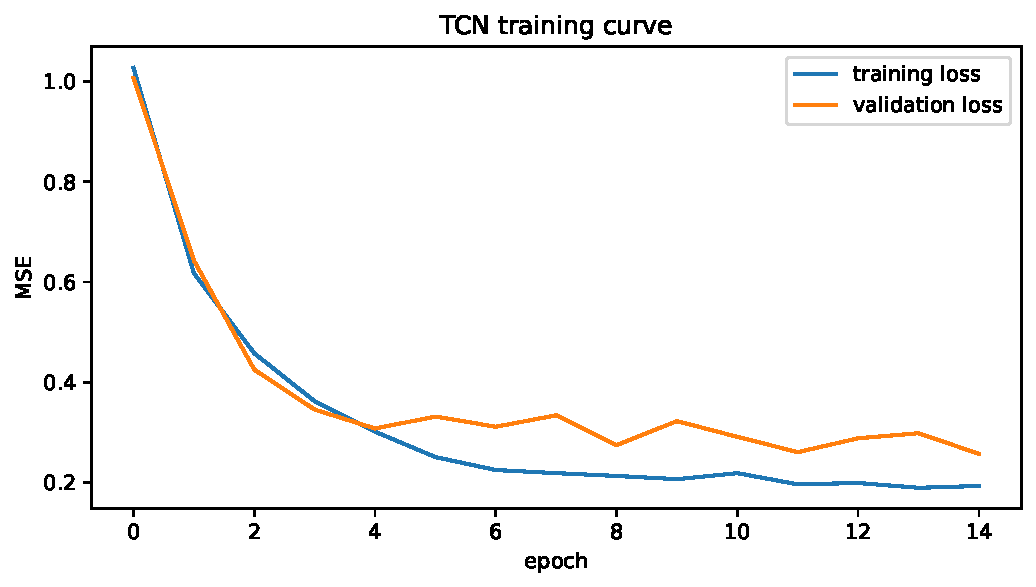
\includegraphics[keepaspectratio]{chapters/chapter-20-convolutional-models-sequences_files/figure-pdf/ch20-tcn-training-output-1.pdf}}

}

\caption{Training and validation loss for a small TCN forecaster.}

\end{figure}%

\begin{verbatim}
Best validation MSE: 0.2570793554186821
\end{verbatim}

Training loss alone is not enough. A useful model should improve
validation loss and beat simple baselines.

\section{20.17 Baseline comparison}\label{baseline-comparison}

A basic multi-step persistence baseline predicts that all future values
equal the last observed value:

\[
\widehat Y_{t+h|t}=Y_t,
\qquad h=1,\ldots,H.
\]

\protect\phantomsection\label{ch20-baseline-comparison}
\begin{Shaded}
\begin{Highlighting}[]
\KeywordTok{def}\NormalTok{ collect\_predictions(loader):}
\NormalTok{    model.}\BuiltInTok{eval}\NormalTok{()}
\NormalTok{    preds }\OperatorTok{=}\NormalTok{ []}
\NormalTok{    targets }\OperatorTok{=}\NormalTok{ []}
\NormalTok{    last\_values }\OperatorTok{=}\NormalTok{ []}
    \ControlFlowTok{with}\NormalTok{ torch.no\_grad():}
        \ControlFlowTok{for}\NormalTok{ xb, yb }\KeywordTok{in}\NormalTok{ loader:}
\NormalTok{            preds.append(model(xb).numpy())}
\NormalTok{            targets.append(yb.numpy())}
\NormalTok{            last\_values.append(xb[:, }\DecValTok{0}\NormalTok{, }\OperatorTok{{-}}\DecValTok{1}\NormalTok{].numpy())}
    \ControlFlowTok{return}\NormalTok{ np.vstack(preds), np.vstack(targets), np.concatenate(last\_values)}

\NormalTok{test\_loader }\OperatorTok{=}\NormalTok{ DataLoader(test\_ds, batch\_size}\OperatorTok{=}\DecValTok{64}\NormalTok{, shuffle}\OperatorTok{=}\VariableTok{False}\NormalTok{)}
\NormalTok{pred\_scaled, target\_scaled, last\_scaled }\OperatorTok{=}\NormalTok{ collect\_predictions(test\_loader)}

\CommentTok{\# Unscale values.}
\NormalTok{pred }\OperatorTok{=}\NormalTok{ pred\_scaled }\OperatorTok{*}\NormalTok{ train\_std }\OperatorTok{+}\NormalTok{ train\_mean}
\NormalTok{target }\OperatorTok{=}\NormalTok{ target\_scaled }\OperatorTok{*}\NormalTok{ train\_std }\OperatorTok{+}\NormalTok{ train\_mean}
\NormalTok{last }\OperatorTok{=}\NormalTok{ last\_scaled }\OperatorTok{*}\NormalTok{ train\_std }\OperatorTok{+}\NormalTok{ train\_mean}
\NormalTok{baseline }\OperatorTok{=}\NormalTok{ np.repeat(last.reshape(}\OperatorTok{{-}}\DecValTok{1}\NormalTok{, }\DecValTok{1}\NormalTok{), H, axis}\OperatorTok{=}\DecValTok{1}\NormalTok{)}

\NormalTok{rmse\_tcn }\OperatorTok{=}\NormalTok{ np.sqrt(np.mean((pred }\OperatorTok{{-}}\NormalTok{ target) }\OperatorTok{**} \DecValTok{2}\NormalTok{, axis}\OperatorTok{=}\DecValTok{0}\NormalTok{))}
\NormalTok{rmse\_base }\OperatorTok{=}\NormalTok{ np.sqrt(np.mean((baseline }\OperatorTok{{-}}\NormalTok{ target) }\OperatorTok{**} \DecValTok{2}\NormalTok{, axis}\OperatorTok{=}\DecValTok{0}\NormalTok{))}

\ControlFlowTok{for}\NormalTok{ h }\KeywordTok{in} \BuiltInTok{range}\NormalTok{(H):}
    \BuiltInTok{print}\NormalTok{(}\SpecialStringTok{f"Horizon }\SpecialCharTok{\{}\NormalTok{h}\OperatorTok{+}\DecValTok{1}\SpecialCharTok{\}}\SpecialStringTok{: TCN RMSE=}\SpecialCharTok{\{}\NormalTok{rmse\_tcn[h]}\SpecialCharTok{:.3f\}}\SpecialStringTok{, persistence RMSE=}\SpecialCharTok{\{}\NormalTok{rmse\_base[h]}\SpecialCharTok{:.3f\}}\SpecialStringTok{"}\NormalTok{)}
\end{Highlighting}
\end{Shaded}

\begin{verbatim}
Horizon 1: TCN RMSE=0.326, persistence RMSE=0.448
Horizon 2: TCN RMSE=0.391, persistence RMSE=0.697
Horizon 3: TCN RMSE=0.399, persistence RMSE=0.882
Horizon 4: TCN RMSE=0.440, persistence RMSE=1.003
Horizon 5: TCN RMSE=0.411, persistence RMSE=1.071
Horizon 6: TCN RMSE=0.406, persistence RMSE=1.100
\end{verbatim}

The goal is not merely to train a CNN. The goal is to show that the CNN
adds predictive value relative to strong baselines.

\begin{Shaded}
\begin{Highlighting}[]
\NormalTok{plt.figure(figsize}\OperatorTok{=}\NormalTok{(}\DecValTok{8}\NormalTok{, }\DecValTok{4}\NormalTok{))}
\NormalTok{plt.plot(np.arange(}\DecValTok{1}\NormalTok{, H }\OperatorTok{+} \DecValTok{1}\NormalTok{), rmse\_tcn, marker}\OperatorTok{=}\StringTok{"o"}\NormalTok{, label}\OperatorTok{=}\StringTok{"TCN"}\NormalTok{)}
\NormalTok{plt.plot(np.arange(}\DecValTok{1}\NormalTok{, H }\OperatorTok{+} \DecValTok{1}\NormalTok{), rmse\_base, marker}\OperatorTok{=}\StringTok{"o"}\NormalTok{, label}\OperatorTok{=}\StringTok{"persistence baseline"}\NormalTok{)}
\NormalTok{plt.xlabel(}\StringTok{"forecast horizon"}\NormalTok{)}
\NormalTok{plt.ylabel(}\StringTok{"RMSE"}\NormalTok{)}
\NormalTok{plt.title(}\StringTok{"Horizon{-}wise test error"}\NormalTok{)}
\NormalTok{plt.legend()}
\NormalTok{plt.show()}
\end{Highlighting}
\end{Shaded}

\begin{figure}[H]

{\centering \pandocbounded{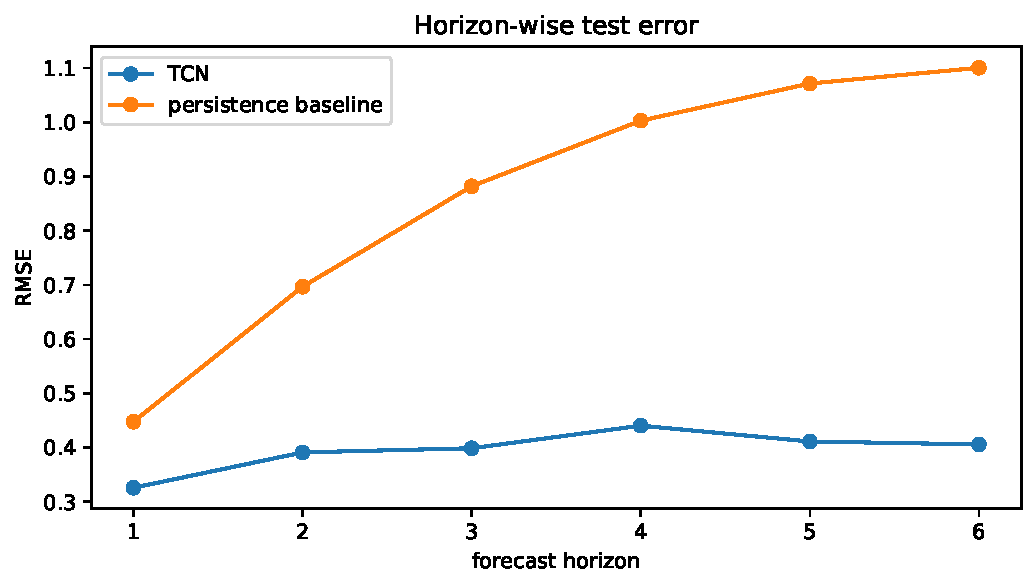
\includegraphics[keepaspectratio]{chapters/chapter-20-convolutional-models-sequences_files/figure-pdf/ch20-horizon-rmse-plot-output-1.pdf}}

}

\caption{Horizon-wise RMSE comparison between the TCN and persistence
baseline.}

\end{figure}%

\section{20.18 Multivariate CNN
forecasting}\label{multivariate-cnn-forecasting}

For multivariate data, the input window is

\[
\mathbf X_t\in\mathbb R^{C\times L}.
\]

A convolutional filter can mix variables and lags at the same time:

\[
z_{t,m}=b_m+
\sum_{c=1}^C\sum_{j=0}^{K-1}W_{m,c,j}x_{t-j,c}.
\]

This is useful when future demand depends on temperature, calendar
variables, promotion indicators, traffic conditions, or sensor
measurements.

However, exogenous variables require careful treatment. Some covariates
are known in advance, such as day of week or scheduled holidays. Others
are unknown at forecast time, such as future temperature unless a
weather forecast is provided. A model must not use future covariates
that would not be available in practice.

\begin{tcolorbox}[enhanced jigsaw, arc=.35mm, bottomrule=.15mm, bottomtitle=1mm, breakable, colback=white, colbacktitle=quarto-callout-warning-color!10!white, colframe=quarto-callout-warning-color-frame, coltitle=black, left=2mm, leftrule=.75mm, opacityback=0, opacitybacktitle=0.6, rightrule=.15mm, title=\textcolor{quarto-callout-warning-color}{\faExclamationTriangle}\hspace{0.5em}{Known future versus unknown future covariates}, titlerule=0mm, toprule=.15mm, toptitle=1mm]

Calendar features are often known for future horizons. Future target
values are not known. Future weather may be known only through a weather
forecast, not through observed future weather. CNN input design must
respect this distinction.

\end{tcolorbox}

\section{20.19 CNNs for classification and anomaly
detection}\label{cnns-for-classification-and-anomaly-detection}

Convolutional sequence models are not only for forecasting. They are
also useful for classification and anomaly detection.

For sequence classification, the model maps

\[
f_\theta:\mathbb R^{C\times L}\to\{1,\ldots,M\}.
\]

Examples include:

\begin{itemize}
\tightlist
\item
  classifying electrocardiogram segments;
\item
  detecting machine faults from vibration signals;
\item
  recognizing activities from accelerometer data;
\item
  identifying regimes from financial or climate sequences.
\end{itemize}

For anomaly detection, a CNN can be trained to reconstruct normal
windows or predict the next observations. Large reconstruction or
prediction errors may indicate abnormal behavior. The threshold should
be calibrated on validation data, not chosen after looking at the test
anomalies.

\section{20.20 Diagnostics and failure
modes}\label{diagnostics-and-failure-modes-1}

A CNN sequence model can fail for several reasons.

\subsection{Receptive field too short}\label{receptive-field-too-short}

If the true dependence uses lags outside the receptive field, the model
cannot use them. Increase \(L\), add layers, increase dilation, or
include known seasonal features.

\subsection{Receptive field too
sparse}\label{receptive-field-too-sparse}

Large dilation can skip important local information. A model with
dilations \(1,2,4,8\) may work well, but a model using only \(d=16\)
might miss short-term patterns.

\subsection{Leakage through padding}\label{leakage-through-padding}

Symmetric padding can use future values. For forecasting, prefer
explicit left padding or carefully verified causal layers.

\subsection{Leakage through
normalization}\label{leakage-through-normalization}

Do not compute scaling constants using validation or test periods. Fit
preprocessing on the training period only.

\subsection{Bad validation design}\label{bad-validation-design}

Randomly splitting overlapping windows can place nearly identical
windows in both training and test sets. Use chronological validation and
rolling-origin evaluation.

\subsection{Overfitting small data}\label{overfitting-small-data}

CNNs can overfit short sequences. Use smaller models, dropout, weight
decay, early stopping, and baselines.

\section{20.21 AI-assisted modeling
activity}\label{ai-assisted-modeling-activity-3}

\section{AI-assisted causality audit}\label{ai-assisted-causality-audit}

Ask an AI assistant:

\begin{quote}
Here is my PyTorch \texttt{Conv1d} code for time-series forecasting.
Audit it for future leakage. Check padding, target construction,
scaling, train-validation split, and use of future covariates. Explain
how to test each issue in code.
\end{quote}

Then verify the answer by writing at least one causality test like the
perturbation test in Section 20.13.

\section{AI-assisted receptive-field
calculation}\label{ai-assisted-receptive-field-calculation}

Use the following prompt:

\begin{quote}
My TCN has kernel size \(K=3\) and dilations \(1,2,4,8,16\). Compute the
receptive-field width. Then explain what historical lags may affect the
final output.
\end{quote}

Check the calculation manually using

\[
R_L=1+(K-1)\sum_{\ell=1}^L d_\ell.
\]

\section{AI-assisted model critique}\label{ai-assisted-model-critique}

Ask an AI assistant to critique a CNN forecasting report. Require it to
answer these questions:

\begin{enumerate}
\def\labelenumi{\arabic{enumi}.}
\tightlist
\item
  What baseline does the CNN beat?
\item
  Is the validation chronological?
\item
  Is the receptive field large enough for the claimed seasonal
  structure?
\item
  Are all future covariates known at forecast time?
\item
  Does the model include uncertainty or only point forecasts?
\end{enumerate}

Reject any suggestion that changes architecture before checking leakage
and baselines.

\section{20.22 Common mistakes}\label{common-mistakes-19}

\begin{enumerate}
\def\labelenumi{\arabic{enumi}.}
\tightlist
\item
  \textbf{Using ordinary symmetric padding for forecasting.} This can
  leak future information.
\item
  \textbf{Forgetting the shape convention.} PyTorch \texttt{Conv1d}
  expects batch, channels, time.
\item
  \textbf{Making the receptive field too small.} The model cannot learn
  dependencies it cannot see.
\item
  \textbf{Using large dilation too early.} Sparse filters can miss local
  patterns.
\item
  \textbf{Skipping baselines.} A CNN must beat naive, seasonal naive,
  and simple ML baselines.
\item
  \textbf{Randomly splitting overlapping windows.} This creates
  misleadingly good test results.
\item
  \textbf{Using future covariates incorrectly.} Only use covariates
  available at forecast time.
\item
  \textbf{Assuming CNNs automatically handle nonstationarity.} Trend,
  scale changes, and regime shifts still require diagnostics.
\item
  \textbf{Training too large a model on too little data.} Deep models
  can memorize local windows.
\item
  \textbf{Reporting only aggregate RMSE.} Horizon-wise error often
  reveals where the model fails.
\end{enumerate}

\section{20.23 Exercises}\label{exercises-19}

\begin{enumerate}
\def\labelenumi{\arabic{enumi}.}
\tightlist
\item
  For a causal convolution with \(K=5\) and \(d=3\), list all input
  times used to compute \(z_t\).
\item
  Prove that a one-layer causal convolution with no activation is a
  finite impulse-response filter.
\item
  For \(K=3\) and dilations \(1,2,4,8\), compute the receptive-field
  width.
\item
  Suppose a series has a weekly seasonal pattern with daily
  observations. Design a TCN receptive field that can see at least four
  weeks of history.
\item
  In PyTorch, explain why the input shape should be
  \texttt{batch,\ channels,\ time} rather than
  \texttt{batch,\ time,\ channels}.
\item
  Write a causality test for a convolutional model by perturbing future
  inputs.
\item
  Modify the Python example to use \(H=12\). How does horizon-wise RMSE
  change?
\item
  Replace ReLU with GELU or Tanh. Does validation loss improve?
\item
  Add a seasonal naive baseline and compare it with the TCN.
\item
  For multivariate forecasting, classify each covariate in your data as
  known future, observed past only, or unavailable.
\end{enumerate}

\section{20.24 Mini project}\label{mini-project-3}

Build a convolutional forecasting model for a real or simulated
sequence.

Your report should include:

\begin{enumerate}
\def\labelenumi{\arabic{enumi}.}
\tightlist
\item
  a forecasting question and horizon;
\item
  a plot of the raw series and at least one diagnostic plot;
\item
  a baseline forecast, preferably naive and seasonal naive;
\item
  a causal CNN or TCN model;
\item
  a calculation of the model's receptive field;
\item
  a chronological train-validation-test split;
\item
  scaling fit on the training period only;
\item
  horizon-wise error comparison;
\item
  a causality audit of your padding and feature construction;
\item
  an AI-assisted critique section where you verify or reject the
  assistant's suggestions.
\end{enumerate}

\section{20.25 Checklist}\label{checklist-4}

Before moving to recurrent networks, make sure you can answer these
questions.

\begin{itemize}
\tightlist
\item
  What is the difference between causal and noncausal convolution?
\item
  What shape does \texttt{Conv1d} expect in PyTorch?
\item
  What is dilation, and why does it increase the receptive field?
\item
  How do you compute the receptive field of a TCN stack?
\item
  What future information is available at forecast time?
\item
  Does your model beat naive and seasonal naive baselines?
\item
  Did you split windows chronologically?
\item
  Was scaling fit on the training period only?
\item
  Can you test whether future inputs affect earlier outputs?
\item
  Can you explain your CNN as a nonlinear time-domain filter?
\end{itemize}

\chapter{Recurrent Neural Networks, LSTM, and
GRU}\label{recurrent-neural-networks-lstm-and-gru}

\textbf{Part VI. Deep Learning for Time Series and Sequence Data}\\
\textbf{Chapter goal:} understand recurrent neural networks for ordered
data. We study hidden states, backpropagation through time, vanishing
and exploding gradients, LSTM gates, GRU gates, forecasting
architectures, validation design, and AI-assisted sequence-model
critique.

\section{Learning objectives}\label{learning-objectives-20}

After studying this chapter, you should be able to:

\begin{enumerate}
\def\labelenumi{\arabic{enumi}.}
\tightlist
\item
  write the mathematical recurrence for a vanilla RNN and interpret the
  hidden state as a learned summary of the past;
\item
  distinguish sequence-to-one, sequence-to-sequence, one-step, and
  multi-step forecasting architectures;
\item
  explain backpropagation through time and why gradients can vanish or
  explode;
\item
  derive the LSTM gate equations and explain the role of the cell state;
\item
  derive the GRU gate equations and compare GRU memory with LSTM memory;
\item
  build RNN, LSTM, and GRU forecasting models in PyTorch using
  leakage-aware time-series splits;
\item
  diagnose whether a recurrent model is improving on simple baselines;
\item
  use AI tools to inspect recurrent-model code while independently
  checking data leakage, tensor shapes, and validation design.
\end{enumerate}

\section{21.1 Motivation: memory in sequence
models}\label{motivation-memory-in-sequence-models}

A feedforward window model predicts from a fixed vector,

\[
(Y_{t-L+1},\ldots,Y_t).
\]

A convolutional model scans learned filters over local neighborhoods. A
recurrent model takes a different approach: it processes the sequence
one step at a time and updates a hidden state. The hidden state is meant
to summarize information from the past that is useful for the current
task.

For a sequence of inputs

\[
\mathbf x_1,\mathbf x_2,\ldots,\mathbf x_T,
\qquad
\mathbf x_t\in\mathbb R^d,
\]

a recurrent model constructs states

\[
\mathbf h_t\in\mathbb R^m,
\]

where \(m\) is the hidden dimension. The state \(\mathbf h_t\) is a
learned representation of the history

\[
\mathcal H_t=(\mathbf x_1,\ldots,\mathbf x_t).
\]

For forecasting, the input might be lagged observations, calendar
features, exogenous covariates, or learned embeddings. For sequence
classification, \(\mathbf h_T\) may summarize the entire sequence. For
sequence-to-sequence prediction, every \(\mathbf h_t\) may produce an
output.

\begin{tcolorbox}[enhanced jigsaw, arc=.35mm, bottomrule=.15mm, bottomtitle=1mm, breakable, colback=white, colbacktitle=quarto-callout-note-color!10!white, colframe=quarto-callout-note-color-frame, coltitle=black, left=2mm, leftrule=.75mm, opacityback=0, opacitybacktitle=0.6, rightrule=.15mm, title=\textcolor{quarto-callout-note-color}{\faInfo}\hspace{0.5em}{Classical connection}, titlerule=0mm, toprule=.15mm, toptitle=1mm]

A recurrent model resembles a nonlinear state-space model. The hidden
state evolves recursively, and predictions are produced from the state.
Unlike a classical state-space model, the transition and observation
maps are learned by gradient descent rather than specified as linear
Gaussian equations.

\end{tcolorbox}

\section{21.2 Vanilla RNN model}\label{vanilla-rnn-model}

The simplest recurrent neural network is

\[
\mathbf h_t = \phi(W_x\mathbf x_t + W_h\mathbf h_{t-1}+\mathbf b_h),
\]

\[
\widehat{\mathbf y}_t = g(W_y\mathbf h_t+\mathbf b_y),
\]

where

\[
W_x\in\mathbb R^{m\times d},
\qquad
W_h\in\mathbb R^{m\times m},
\qquad
W_y\in\mathbb R^{r\times m}.
\]

Here \(\phi\) is usually a nonlinear activation such as \(\tanh\) or
ReLU, and \(g\) depends on the task. For regression, \(g\) is often the
identity map. For classification, \(g\) may be a sigmoid or softmax map.

The same matrices \(W_x,W_h,W_y\) are reused at every time step. This
weight sharing is the central structural assumption of a vanilla RNN. It
says that the same local update rule is applied throughout the sequence.

For a univariate time series, a scalar version is

\[
h_t=\phi(a h_{t-1}+b x_t+c),
\qquad
\widehat y_t=w h_t+d.
\]

If \(\phi\) is the identity and \(c=0\), then

\[
h_t=a h_{t-1}+b x_t.
\]

Iterating gives

\[
h_t=b x_t+ab x_{t-1}+a^2b x_{t-2}+\cdots+a^{t-1}b x_1+a^t h_0.
\]

Thus the recurrent weight \(a\) controls memory. If \(|a|<1\), the
remote past is exponentially downweighted. If \(|a|>1\), the state may
explode. Nonlinear activations moderate this behavior, but the same
intuition remains important.

\section{21.3 Computational graph and backpropagation through
time}\label{computational-graph-and-backpropagation-through-time}

Training a recurrent model means minimizing a loss over time. For a
forecasting problem, a common loss is

\[
\mathcal L(\Theta)=\frac{1}{N}\sum_{i=1}^N\sum_{t\in \mathcal T_i}
\ell(\widehat y_{i,t},y_{i,t}),
\]

where \(i\) indexes training windows or sequences. For squared-error
forecasting,

\[
\ell(\widehat y_{i,t},y_{i,t})=(\widehat y_{i,t}-y_{i,t})^2.
\]

The RNN is a composition of repeated maps. To compute gradients, we
unroll the recurrence through time and apply the chain rule. This is
called \textbf{backpropagation through time}.

For the vanilla RNN,

\[
\mathbf a_t=W_x\mathbf x_t+W_h\mathbf h_{t-1}+\mathbf b_h,
\qquad
\mathbf h_t=\phi(\mathbf a_t).
\]

The Jacobian of \(\mathbf h_t\) with respect to \(\mathbf h_{t-1}\) is

\[
\frac{\partial \mathbf h_t}{\partial \mathbf h_{t-1}}
=
D_t W_h,
\]

where

\[
D_t=\operatorname{diag}(\phi'(\mathbf a_t)).
\]

Therefore, the sensitivity of a later state to an earlier state contains
products such as

\[
\frac{\partial \mathbf h_t}{\partial \mathbf h_{t-k}}
=
(D_t W_h)(D_{t-1}W_h)\cdots(D_{t-k+1}W_h).
\]

This product explains the \textbf{vanishing gradient} and
\textbf{exploding gradient} problems. If these matrices repeatedly
shrink vectors, gradients vanish and the model has difficulty learning
long-range dependence. If they repeatedly expand vectors, gradients
explode and training becomes unstable.

\begin{tcolorbox}[enhanced jigsaw, arc=.35mm, bottomrule=.15mm, bottomtitle=1mm, breakable, colback=white, colbacktitle=quarto-callout-warning-color!10!white, colframe=quarto-callout-warning-color-frame, coltitle=black, left=2mm, leftrule=.75mm, opacityback=0, opacitybacktitle=0.6, rightrule=.15mm, title=\textcolor{quarto-callout-warning-color}{\faExclamationTriangle}\hspace{0.5em}{Practical consequence}, titlerule=0mm, toprule=.15mm, toptitle=1mm]

A vanilla RNN can work well for short memory. For long memory, LSTM,
GRU, attention, temporal convolutional networks, or state-space sequence
models often train more reliably.

\end{tcolorbox}

\section{21.4 Forecasting
architectures}\label{forecasting-architectures}

There are several ways to use recurrent networks for forecasting.

\subsection{Sequence-to-one
forecasting}\label{sequence-to-one-forecasting}

A window

\[
(Y_{t-L+1},\ldots,Y_t)
\]

is fed into the recurrent network, and the final hidden state
\(\mathbf h_L\) is used to predict one or more future values:

\[
(\widehat Y_{t+1},\ldots,\widehat Y_{t+H})=F_\Theta(\mathbf h_L).
\]

This is common for direct multi-horizon forecasting.

\subsection{Sequence-to-sequence
forecasting}\label{sequence-to-sequence-forecasting}

The model produces an output at each input time or each decoder time:

\[
\widehat Y_t=g(W_y\mathbf h_t+\mathbf b_y).
\]

For multi-step forecasting, an encoder RNN can summarize the observed
history, and a decoder RNN can generate the future path.

\subsection{Recursive forecasting}\label{recursive-forecasting}

A one-step model predicts

\[
\widehat Y_{t+1}=F_\Theta(Y_{t-L+1},\ldots,Y_t),
\]

then feeds its own prediction back into the input window to predict
\(\widehat Y_{t+2}\), and so on. Recursive forecasting is simple but can
accumulate error.

\subsection{Teacher forcing}\label{teacher-forcing}

During sequence-to-sequence training, the decoder can be given the true
previous value instead of its own previous prediction. This is called
teacher forcing. It stabilizes training, but creates a mismatch between
training and deployment. At deployment time, future true values are
unavailable.

\section{21.5 LSTM: long short-term
memory}\label{lstm-long-short-term-memory}

The LSTM was designed to make long-range memory easier to train. It
maintains two states:

\[
\mathbf h_t \quad \text{hidden state},
\qquad
\mathbf c_t \quad \text{cell state}.
\]

A common LSTM formulation is

\[
\mathbf f_t=\sigma(W_f\mathbf x_t+U_f\mathbf h_{t-1}+\mathbf b_f),
\]

\[
\mathbf i_t=\sigma(W_i\mathbf x_t+U_i\mathbf h_{t-1}+\mathbf b_i),
\]

\[
\widetilde{\mathbf c}_t=\tanh(W_c\mathbf x_t+U_c\mathbf h_{t-1}+\mathbf b_c),
\]

\[
\mathbf c_t=\mathbf f_t\odot \mathbf c_{t-1}+\mathbf i_t\odot\widetilde{\mathbf c}_t,
\]

\[
\mathbf o_t=\sigma(W_o\mathbf x_t+U_o\mathbf h_{t-1}+\mathbf b_o),
\]

\[
\mathbf h_t=\mathbf o_t\odot \tanh(\mathbf c_t).
\]

The symbols have the following meanings:

\begin{itemize}
\tightlist
\item
  \(\mathbf f_t\) is the \textbf{forget gate};
\item
  \(\mathbf i_t\) is the \textbf{input gate};
\item
  \(\widetilde{\mathbf c}_t\) is the candidate memory;
\item
  \(\mathbf o_t\) is the \textbf{output gate};
\item
  \(\odot\) denotes componentwise multiplication.
\end{itemize}

The cell-state equation

\[
\mathbf c_t=\mathbf f_t\odot \mathbf c_{t-1}+\mathbf i_t\odot\widetilde{\mathbf c}_t
\]

is the core idea. It creates a path along which information can be
retained, forgotten, or updated. When a component of \(\mathbf f_t\) is
close to \(1\) and the corresponding component of \(\mathbf i_t\) is
close to \(0\), that component of memory is carried forward with little
change.

\section{21.6 GRU: gated recurrent unit}\label{gru-gated-recurrent-unit}

A GRU is a simpler gated recurrent architecture. It uses an update gate
and a reset gate. A common formulation is

\[
\mathbf z_t=\sigma(W_z\mathbf x_t+U_z\mathbf h_{t-1}+\mathbf b_z),
\]

\[
\mathbf r_t=\sigma(W_r\mathbf x_t+U_r\mathbf h_{t-1}+\mathbf b_r),
\]

\[
\widetilde{\mathbf h}_t=\tanh(W_h\mathbf x_t+U_h(\mathbf r_t\odot \mathbf h_{t-1})+\mathbf b_h),
\]

\[
\mathbf h_t=(1-\mathbf z_t)\odot \mathbf h_{t-1}+\mathbf z_t\odot\widetilde{\mathbf h}_t.
\]

The update gate \(\mathbf z_t\) controls how much the state changes. If
\(\mathbf z_t\) is near \(0\), the previous state is mostly retained. If
\(\mathbf z_t\) is near \(1\), the candidate state mostly replaces the
previous state. The reset gate \(\mathbf r_t\) controls how much of the
previous state is used when constructing the candidate state.

\begin{tcolorbox}[enhanced jigsaw, arc=.35mm, bottomrule=.15mm, bottomtitle=1mm, breakable, colback=white, colbacktitle=quarto-callout-tip-color!10!white, colframe=quarto-callout-tip-color-frame, coltitle=black, left=2mm, leftrule=.75mm, opacityback=0, opacitybacktitle=0.6, rightrule=.15mm, title=\textcolor{quarto-callout-tip-color}{\faLightbulb}\hspace{0.5em}{LSTM versus GRU}, titlerule=0mm, toprule=.15mm, toptitle=1mm]

LSTMs have separate hidden and cell states and more gates. GRUs are
simpler and often faster. There is no universal winner. In applied
forecasting, compare both against strong baselines using the same
chronological validation design.

\end{tcolorbox}

\section{21.7 Data windows and tensor
shapes}\label{data-windows-and-tensor-shapes}

In PyTorch, recurrent layers commonly use a tensor shape

\[
\text{batch size}\times \text{sequence length}\times \text{number of features}
\]

when \texttt{batch\_first=True}. For univariate forecasting with input
length \(L\), a batch of \(B\) windows has shape

\[
B\times L\times 1.
\]

For direct \(H\)-step forecasting, the target may have shape

\[
B\times H.
\]

A clean supervised construction is

\[
\mathbf X_i=(Y_i,Y_{i+1},\ldots,Y_{i+L-1}),
\]

\[
\mathbf y_i=(Y_{i+L},Y_{i+L+1},\ldots,Y_{i+L+H-1}).
\]

The split between training, validation, and test data must respect time
order. Scaling parameters should be fit on the training portion only.

\section{21.8 Interactive module: vanilla RNN hidden-state
dynamics}\label{interactive-module-vanilla-rnn-hidden-state-dynamics}

This module shows how the recurrent weight and input weight influence
memory. The scalar recurrence is

\[
h_t=\phi(a h_{t-1}+b x_t).
\]

Large positive \(a\) creates persistence, negative \(a\) creates
oscillatory sign changes, and \(|a|>1\) can cause instability when the
activation is linear.

Interactive Module 21.1: RNN Hidden-State Dynamics

Change the recurrent weight, input weight, activation, and input
pattern. The Plotly toolbar is enabled globally: zoom, pan, reset,
autoscale, and download are available.

\begin{verbatim}
<label>Recurrent weight $a$
  <input id="ch21_rnn_a" type="range" min="-1.4" max="1.4" step="0.05" value="0.65">
  <span id="ch21_rnn_a_value">0.65</span>
</label>

<label>Input weight $b$
  <input id="ch21_rnn_b" type="range" min="0" max="2" step="0.05" value="0.85">
  <span id="ch21_rnn_b_value">0.85</span>
</label>

<label>Activation
  <select id="ch21_rnn_activation">
    <option value="tanh" selected>tanh</option>
    <option value="linear">linear</option>
    <option value="relu">ReLU</option>
  </select>
</label>

<label>Input pattern
  <select id="ch21_rnn_input">
    <option value="pulse" selected>pulse + seasonal</option>
    <option value="sine">smooth sine wave</option>
    <option value="step">step change</option>
    <option value="alternating">alternating signs</option>
  </select>
</label>
\end{verbatim}

\protect\phantomsection\label{ch21_rnn_state_plot}

\section{21.9 Interactive module: gated memory in LSTM and
GRU}\label{interactive-module-gated-memory-in-lstm-and-gru}

The next module gives a simplified gate-level view. The gates are fixed
sliders rather than learned functions of \(x_t\) and \(h_{t-1}\). This
is not a full trained LSTM or GRU; it is a controlled visualization of
what the gates do.

For the LSTM view, the scalar equations are

\[
c_t=f c_{t-1}+i\widetilde c_t,
\qquad
h_t=o\tanh(c_t).
\]

For the GRU view, the scalar equations are

\[
\widetilde h_t=\tanh(gx_t+r h_{t-1}),
\qquad
h_t=(1-z)h_{t-1}+z\widetilde h_t.
\]

Interactive Module 21.2: LSTM/GRU Gate Explorer

Use the sliders to see how gated recurrence stores, overwrites, or
exposes memory.

\begin{verbatim}
<label>Model
  <select id="ch21_gate_model">
    <option value="lstm" selected>LSTM simplified gates</option>
    <option value="gru">GRU simplified gates</option>
  </select>
</label>

<label><span id="ch21_gate1_label">Forget gate $f$</span>
  <input id="ch21_gate1" type="range" min="0" max="1" step="0.02" value="0.88">
  <span id="ch21_gate1_value">0.88</span>
</label>

<label><span id="ch21_gate2_label">Input gate $i$</span>
  <input id="ch21_gate2" type="range" min="0" max="1" step="0.02" value="0.35">
  <span id="ch21_gate2_value">0.35</span>
</label>

<label><span id="ch21_gate3_label">Output gate $o$</span>
  <input id="ch21_gate3" type="range" min="0" max="1" step="0.02" value="0.80">
  <span id="ch21_gate3_value">0.80</span>
</label>

<label>Candidate input gain $g$
  <input id="ch21_gate_gain" type="range" min="0" max="3" step="0.05" value="1.25">
  <span id="ch21_gate_gain_value">1.25</span>
</label>
\end{verbatim}

\protect\phantomsection\label{ch21_gate_plot}

\section{21.10 Python example: building supervised sequence
windows}\label{python-example-building-supervised-sequence-windows}

The first implementation step is not the neural network. It is the
supervised-learning data set.

\begin{Shaded}
\begin{Highlighting}[]
\ImportTok{import}\NormalTok{ numpy }\ImportTok{as}\NormalTok{ np}
\ImportTok{import}\NormalTok{ matplotlib.pyplot }\ImportTok{as}\NormalTok{ plt}

\NormalTok{rng }\OperatorTok{=}\NormalTok{ np.random.default\_rng(}\DecValTok{21}\NormalTok{)}
\NormalTok{T }\OperatorTok{=} \DecValTok{420}
\NormalTok{t }\OperatorTok{=}\NormalTok{ np.arange(T)}

\NormalTok{signal }\OperatorTok{=}\NormalTok{ (}
    \FloatTok{0.012} \OperatorTok{*}\NormalTok{ t}
    \OperatorTok{+} \FloatTok{1.4} \OperatorTok{*}\NormalTok{ np.sin(}\DecValTok{2} \OperatorTok{*}\NormalTok{ np.pi }\OperatorTok{*}\NormalTok{ t }\OperatorTok{/} \DecValTok{32}\NormalTok{)}
    \OperatorTok{+} \FloatTok{0.6} \OperatorTok{*}\NormalTok{ np.sin(}\DecValTok{2} \OperatorTok{*}\NormalTok{ np.pi }\OperatorTok{*}\NormalTok{ t }\OperatorTok{/} \DecValTok{9}\NormalTok{)}
\NormalTok{)}
\NormalTok{noise }\OperatorTok{=}\NormalTok{ rng.normal(scale}\OperatorTok{=}\FloatTok{0.35}\NormalTok{, size}\OperatorTok{=}\NormalTok{T)}
\NormalTok{y }\OperatorTok{=}\NormalTok{ signal }\OperatorTok{+}\NormalTok{ noise}

\NormalTok{L }\OperatorTok{=} \DecValTok{36}     \CommentTok{\# input length}
\NormalTok{H }\OperatorTok{=} \DecValTok{6}      \CommentTok{\# forecast horizon}

\NormalTok{X, Y }\OperatorTok{=}\NormalTok{ [], []}
\ControlFlowTok{for}\NormalTok{ start }\KeywordTok{in} \BuiltInTok{range}\NormalTok{(T }\OperatorTok{{-}}\NormalTok{ L }\OperatorTok{{-}}\NormalTok{ H }\OperatorTok{+} \DecValTok{1}\NormalTok{):}
\NormalTok{    X.append(y[start:start }\OperatorTok{+}\NormalTok{ L])}
\NormalTok{    Y.append(y[start }\OperatorTok{+}\NormalTok{ L:start }\OperatorTok{+}\NormalTok{ L }\OperatorTok{+}\NormalTok{ H])}

\NormalTok{X }\OperatorTok{=}\NormalTok{ np.array(X)}
\NormalTok{Y }\OperatorTok{=}\NormalTok{ np.array(Y)}

\BuiltInTok{print}\NormalTok{(}\StringTok{"X shape:"}\NormalTok{, X.shape)  }\CommentTok{\# windows x input length}
\BuiltInTok{print}\NormalTok{(}\StringTok{"Y shape:"}\NormalTok{, Y.shape)  }\CommentTok{\# windows x forecast horizon}

\NormalTok{plt.figure(figsize}\OperatorTok{=}\NormalTok{(}\DecValTok{8}\NormalTok{, }\FloatTok{3.5}\NormalTok{))}
\NormalTok{plt.plot(t, y, label}\OperatorTok{=}\StringTok{"observed"}\NormalTok{)}
\NormalTok{plt.axvspan(}\DecValTok{0}\NormalTok{, }\DecValTok{300}\NormalTok{, alpha}\OperatorTok{=}\FloatTok{0.15}\NormalTok{, label}\OperatorTok{=}\StringTok{"training region"}\NormalTok{)}
\NormalTok{plt.xlabel(}\StringTok{"time"}\NormalTok{)}
\NormalTok{plt.ylabel(}\StringTok{"value"}\NormalTok{)}
\NormalTok{plt.title(}\StringTok{"Synthetic sequence for recurrent forecasting"}\NormalTok{)}
\NormalTok{plt.legend()}
\NormalTok{plt.show()}
\end{Highlighting}
\end{Shaded}

\begin{verbatim}
X shape: (379, 36)
Y shape: (379, 6)
\end{verbatim}

\begin{figure}[H]

{\centering \pandocbounded{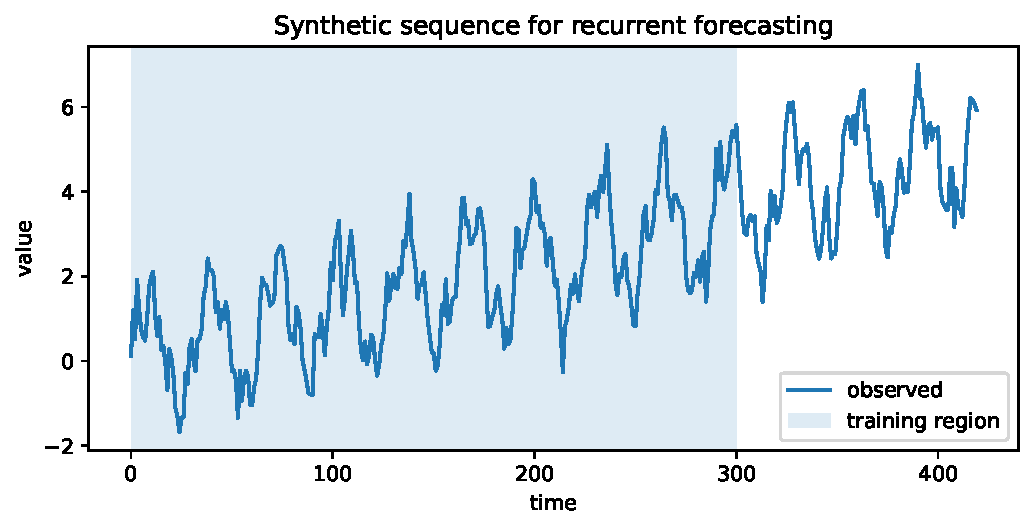
\includegraphics[keepaspectratio]{chapters/chapter-21-rnn-lstm-gru_files/figure-pdf/ch21-window-dataset-output-2.pdf}}

}

\caption{Synthetic time series used for RNN, LSTM, and GRU examples.}

\end{figure}%

\section{21.11 Python example: leakage-aware scaling and chronological
split}\label{python-example-leakage-aware-scaling-and-chronological-split}

We split windows by their forecast origin. Scaling uses only the
training windows.

\protect\phantomsection\label{ch21-split-scale}
\begin{Shaded}
\begin{Highlighting}[]
\ImportTok{from}\NormalTok{ sklearn.preprocessing }\ImportTok{import}\NormalTok{ StandardScaler}

\NormalTok{n\_windows }\OperatorTok{=} \BuiltInTok{len}\NormalTok{(X)}
\NormalTok{train\_end }\OperatorTok{=} \BuiltInTok{int}\NormalTok{(}\FloatTok{0.70} \OperatorTok{*}\NormalTok{ n\_windows)}
\NormalTok{val\_end }\OperatorTok{=} \BuiltInTok{int}\NormalTok{(}\FloatTok{0.85} \OperatorTok{*}\NormalTok{ n\_windows)}

\NormalTok{X\_train, Y\_train }\OperatorTok{=}\NormalTok{ X[:train\_end], Y[:train\_end]}
\NormalTok{X\_val, Y\_val }\OperatorTok{=}\NormalTok{ X[train\_end:val\_end], Y[train\_end:val\_end]}
\NormalTok{X\_test, Y\_test }\OperatorTok{=}\NormalTok{ X[val\_end:], Y[val\_end:]}

\NormalTok{x\_scaler }\OperatorTok{=}\NormalTok{ StandardScaler()}
\NormalTok{y\_scaler }\OperatorTok{=}\NormalTok{ StandardScaler()}

\NormalTok{X\_train\_scaled }\OperatorTok{=}\NormalTok{ x\_scaler.fit\_transform(X\_train.reshape(}\OperatorTok{{-}}\DecValTok{1}\NormalTok{, }\DecValTok{1}\NormalTok{)).reshape(X\_train.shape)}
\NormalTok{X\_val\_scaled }\OperatorTok{=}\NormalTok{ x\_scaler.transform(X\_val.reshape(}\OperatorTok{{-}}\DecValTok{1}\NormalTok{, }\DecValTok{1}\NormalTok{)).reshape(X\_val.shape)}
\NormalTok{X\_test\_scaled }\OperatorTok{=}\NormalTok{ x\_scaler.transform(X\_test.reshape(}\OperatorTok{{-}}\DecValTok{1}\NormalTok{, }\DecValTok{1}\NormalTok{)).reshape(X\_test.shape)}

\NormalTok{Y\_train\_scaled }\OperatorTok{=}\NormalTok{ y\_scaler.fit\_transform(Y\_train.reshape(}\OperatorTok{{-}}\DecValTok{1}\NormalTok{, }\DecValTok{1}\NormalTok{)).reshape(Y\_train.shape)}
\NormalTok{Y\_val\_scaled }\OperatorTok{=}\NormalTok{ y\_scaler.transform(Y\_val.reshape(}\OperatorTok{{-}}\DecValTok{1}\NormalTok{, }\DecValTok{1}\NormalTok{)).reshape(Y\_val.shape)}
\NormalTok{Y\_test\_scaled }\OperatorTok{=}\NormalTok{ y\_scaler.transform(Y\_test.reshape(}\OperatorTok{{-}}\DecValTok{1}\NormalTok{, }\DecValTok{1}\NormalTok{)).reshape(Y\_test.shape)}

\BuiltInTok{print}\NormalTok{(}\StringTok{"train/val/test windows:"}\NormalTok{, }\BuiltInTok{len}\NormalTok{(X\_train), }\BuiltInTok{len}\NormalTok{(X\_val), }\BuiltInTok{len}\NormalTok{(X\_test))}
\end{Highlighting}
\end{Shaded}

\begin{verbatim}
train/val/test windows: 265 57 57
\end{verbatim}

\section{21.12 Python example: RNN direct multi-horizon
forecaster}\label{python-example-rnn-direct-multi-horizon-forecaster}

The following model reads a length-\(L\) sequence and predicts the next
\(H\) values from the last hidden state.

\begin{Shaded}
\begin{Highlighting}[]
\ImportTok{import}\NormalTok{ torch}
\ImportTok{from}\NormalTok{ torch }\ImportTok{import}\NormalTok{ nn}
\ImportTok{from}\NormalTok{ torch.utils.data }\ImportTok{import}\NormalTok{ TensorDataset, DataLoader}
\ImportTok{from}\NormalTok{ sklearn.metrics }\ImportTok{import}\NormalTok{ mean\_squared\_error}

\NormalTok{np.random.seed(}\DecValTok{21}\NormalTok{)}
\NormalTok{torch.manual\_seed(}\DecValTok{21}\NormalTok{)}

\KeywordTok{def}\NormalTok{ to\_tensor\_windows(A):}
    \ControlFlowTok{return}\NormalTok{ torch.tensor(A, dtype}\OperatorTok{=}\NormalTok{torch.float32).unsqueeze(}\OperatorTok{{-}}\DecValTok{1}\NormalTok{)}

\KeywordTok{def}\NormalTok{ to\_tensor\_targets(A):}
    \ControlFlowTok{return}\NormalTok{ torch.tensor(A, dtype}\OperatorTok{=}\NormalTok{torch.float32)}

\NormalTok{train\_ds }\OperatorTok{=}\NormalTok{ TensorDataset(to\_tensor\_windows(X\_train\_scaled), to\_tensor\_targets(Y\_train\_scaled))}
\NormalTok{val\_ds }\OperatorTok{=}\NormalTok{ TensorDataset(to\_tensor\_windows(X\_val\_scaled), to\_tensor\_targets(Y\_val\_scaled))}
\NormalTok{test\_ds }\OperatorTok{=}\NormalTok{ TensorDataset(to\_tensor\_windows(X\_test\_scaled), to\_tensor\_targets(Y\_test\_scaled))}

\NormalTok{train\_loader }\OperatorTok{=}\NormalTok{ DataLoader(train\_ds, batch\_size}\OperatorTok{=}\DecValTok{32}\NormalTok{, shuffle}\OperatorTok{=}\VariableTok{True}\NormalTok{)}
\NormalTok{val\_loader }\OperatorTok{=}\NormalTok{ DataLoader(val\_ds, batch\_size}\OperatorTok{=}\DecValTok{64}\NormalTok{, shuffle}\OperatorTok{=}\VariableTok{False}\NormalTok{)}

\KeywordTok{class}\NormalTok{ RNNForecaster(nn.Module):}
    \KeywordTok{def} \FunctionTok{\_\_init\_\_}\NormalTok{(}\VariableTok{self}\NormalTok{, hidden\_size}\OperatorTok{=}\DecValTok{24}\NormalTok{, horizon}\OperatorTok{=}\DecValTok{6}\NormalTok{):}
        \BuiltInTok{super}\NormalTok{().}\FunctionTok{\_\_init\_\_}\NormalTok{()}
        \VariableTok{self}\NormalTok{.rnn }\OperatorTok{=}\NormalTok{ nn.RNN(}
\NormalTok{            input\_size}\OperatorTok{=}\DecValTok{1}\NormalTok{,}
\NormalTok{            hidden\_size}\OperatorTok{=}\NormalTok{hidden\_size,}
\NormalTok{            num\_layers}\OperatorTok{=}\DecValTok{1}\NormalTok{,}
\NormalTok{            nonlinearity}\OperatorTok{=}\StringTok{"tanh"}\NormalTok{,}
\NormalTok{            batch\_first}\OperatorTok{=}\VariableTok{True}
\NormalTok{        )}
        \VariableTok{self}\NormalTok{.head }\OperatorTok{=}\NormalTok{ nn.Linear(hidden\_size, horizon)}

    \KeywordTok{def}\NormalTok{ forward(}\VariableTok{self}\NormalTok{, x):}
\NormalTok{        out, h\_last }\OperatorTok{=} \VariableTok{self}\NormalTok{.rnn(x)}
\NormalTok{        last\_hidden }\OperatorTok{=}\NormalTok{ out[:, }\OperatorTok{{-}}\DecValTok{1}\NormalTok{, :]}
        \ControlFlowTok{return} \VariableTok{self}\NormalTok{.head(last\_hidden)}

\NormalTok{model }\OperatorTok{=}\NormalTok{ RNNForecaster(hidden\_size}\OperatorTok{=}\DecValTok{24}\NormalTok{, horizon}\OperatorTok{=}\NormalTok{H)}
\NormalTok{optimizer }\OperatorTok{=}\NormalTok{ torch.optim.Adam(model.parameters(), lr}\OperatorTok{=}\FloatTok{0.01}\NormalTok{)}
\NormalTok{loss\_fn }\OperatorTok{=}\NormalTok{ nn.MSELoss()}

\ControlFlowTok{for}\NormalTok{ epoch }\KeywordTok{in} \BuiltInTok{range}\NormalTok{(}\DecValTok{8}\NormalTok{):}
\NormalTok{    model.train()}
\NormalTok{    train\_losses }\OperatorTok{=}\NormalTok{ []}
    \ControlFlowTok{for}\NormalTok{ xb, yb }\KeywordTok{in}\NormalTok{ train\_loader:}
\NormalTok{        optimizer.zero\_grad()}
\NormalTok{        pred }\OperatorTok{=}\NormalTok{ model(xb)}
\NormalTok{        loss }\OperatorTok{=}\NormalTok{ loss\_fn(pred, yb)}
\NormalTok{        loss.backward()}
\NormalTok{        torch.nn.utils.clip\_grad\_norm\_(model.parameters(), max\_norm}\OperatorTok{=}\FloatTok{1.0}\NormalTok{)}
\NormalTok{        optimizer.step()}
\NormalTok{        train\_losses.append(loss.item())}

\NormalTok{    model.}\BuiltInTok{eval}\NormalTok{()}
\NormalTok{    val\_losses }\OperatorTok{=}\NormalTok{ []}
    \ControlFlowTok{with}\NormalTok{ torch.no\_grad():}
        \ControlFlowTok{for}\NormalTok{ xb, yb }\KeywordTok{in}\NormalTok{ val\_loader:}
\NormalTok{            val\_losses.append(loss\_fn(model(xb), yb).item())}

    \BuiltInTok{print}\NormalTok{(}\SpecialStringTok{f"epoch }\SpecialCharTok{\{}\NormalTok{epoch }\OperatorTok{+} \DecValTok{1}\SpecialCharTok{:02d\}}\SpecialStringTok{ | train MSE }\SpecialCharTok{\{}\NormalTok{np}\SpecialCharTok{.}\NormalTok{mean(train\_losses)}\SpecialCharTok{:.4f\}}\SpecialStringTok{ | val MSE }\SpecialCharTok{\{}\NormalTok{np}\SpecialCharTok{.}\NormalTok{mean(val\_losses)}\SpecialCharTok{:.4f\}}\SpecialStringTok{"}\NormalTok{)}

\NormalTok{model.}\BuiltInTok{eval}\NormalTok{()}
\ControlFlowTok{with}\NormalTok{ torch.no\_grad():}
\NormalTok{    pred\_scaled }\OperatorTok{=}\NormalTok{ model(to\_tensor\_windows(X\_test\_scaled)).numpy()}

\NormalTok{pred }\OperatorTok{=}\NormalTok{ y\_scaler.inverse\_transform(pred\_scaled.reshape(}\OperatorTok{{-}}\DecValTok{1}\NormalTok{, }\DecValTok{1}\NormalTok{)).reshape(pred\_scaled.shape)}
\NormalTok{rmse }\OperatorTok{=}\NormalTok{ mean\_squared\_error(Y\_test.ravel(), pred.ravel()) }\OperatorTok{**} \FloatTok{0.5}
\BuiltInTok{print}\NormalTok{(}\StringTok{"test RMSE:"}\NormalTok{, }\BuiltInTok{round}\NormalTok{(rmse, }\DecValTok{3}\NormalTok{))}

\NormalTok{idx }\OperatorTok{=} \DecValTok{4}
\NormalTok{history }\OperatorTok{=}\NormalTok{ X\_test[idx]}
\NormalTok{truth }\OperatorTok{=}\NormalTok{ Y\_test[idx]}
\NormalTok{forecast }\OperatorTok{=}\NormalTok{ pred[idx]}

\NormalTok{plt.figure(figsize}\OperatorTok{=}\NormalTok{(}\DecValTok{8}\NormalTok{, }\FloatTok{3.5}\NormalTok{))}
\NormalTok{plt.plot(np.arange(L), history, label}\OperatorTok{=}\StringTok{"history"}\NormalTok{)}
\NormalTok{plt.plot(np.arange(L, L }\OperatorTok{+}\NormalTok{ H), truth, marker}\OperatorTok{=}\StringTok{"o"}\NormalTok{, label}\OperatorTok{=}\StringTok{"future truth"}\NormalTok{)}
\NormalTok{plt.plot(np.arange(L, L }\OperatorTok{+}\NormalTok{ H), forecast, marker}\OperatorTok{=}\StringTok{"o"}\NormalTok{, label}\OperatorTok{=}\StringTok{"RNN forecast"}\NormalTok{)}
\NormalTok{plt.axvline(L }\OperatorTok{{-}} \FloatTok{0.5}\NormalTok{, linestyle}\OperatorTok{=}\StringTok{"{-}{-}"}\NormalTok{, linewidth}\OperatorTok{=}\DecValTok{1}\NormalTok{)}
\NormalTok{plt.xlabel(}\StringTok{"relative time"}\NormalTok{)}
\NormalTok{plt.ylabel(}\StringTok{"value"}\NormalTok{)}
\NormalTok{plt.title(}\StringTok{"Direct multi{-}horizon RNN forecast"}\NormalTok{)}
\NormalTok{plt.legend()}
\NormalTok{plt.show()}
\end{Highlighting}
\end{Shaded}

\begin{verbatim}
epoch 01 | train MSE 0.7808 | val MSE 0.8689
epoch 02 | train MSE 0.5299 | val MSE 0.7937
epoch 03 | train MSE 0.4946 | val MSE 0.7270
epoch 04 | train MSE 0.4741 | val MSE 0.7193
epoch 05 | train MSE 0.4687 | val MSE 0.7406
epoch 06 | train MSE 0.4765 | val MSE 0.7681
epoch 07 | train MSE 0.4545 | val MSE 0.6382
epoch 08 | train MSE 0.4132 | val MSE 0.5828
test RMSE: 1.22
\end{verbatim}

\begin{figure}[H]

{\centering \pandocbounded{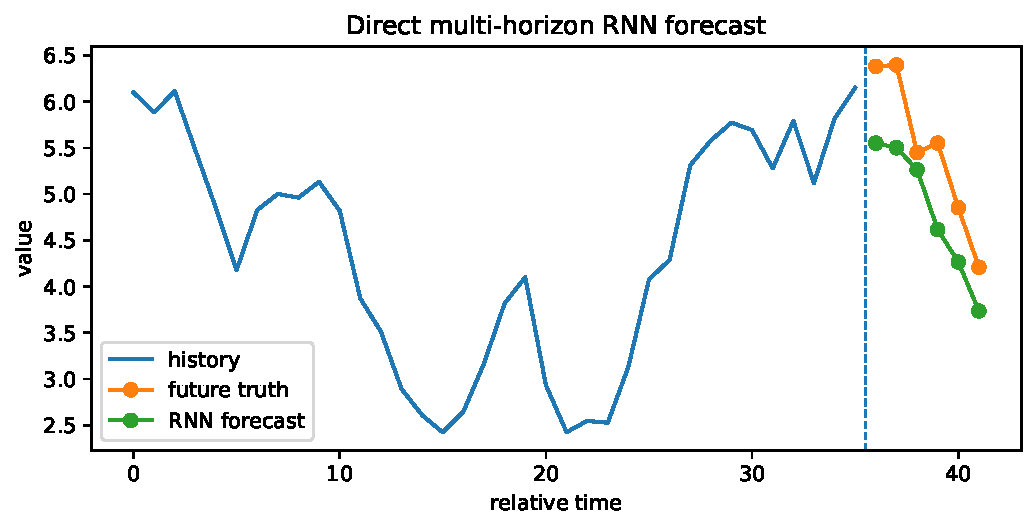
\includegraphics[keepaspectratio]{chapters/chapter-21-rnn-lstm-gru_files/figure-pdf/ch21-rnn-pytorch-output-2.pdf}}

}

\caption{RNN direct multi-horizon forecast on a held-out test window.}

\end{figure}%

\section{21.13 Python example: swapping RNN, LSTM, and GRU
cells}\label{python-example-swapping-rnn-lstm-and-gru-cells}

The same forecasting head can be used with \texttt{nn.RNN},
\texttt{nn.LSTM}, or \texttt{nn.GRU}.

\protect\phantomsection\label{ch21-cell-comparison}
\begin{Shaded}
\begin{Highlighting}[]
\KeywordTok{class}\NormalTok{ RecurrentForecaster(nn.Module):}
    \KeywordTok{def} \FunctionTok{\_\_init\_\_}\NormalTok{(}\VariableTok{self}\NormalTok{, cell}\OperatorTok{=}\StringTok{"gru"}\NormalTok{, hidden\_size}\OperatorTok{=}\DecValTok{24}\NormalTok{, horizon}\OperatorTok{=}\DecValTok{6}\NormalTok{):}
        \BuiltInTok{super}\NormalTok{().}\FunctionTok{\_\_init\_\_}\NormalTok{()}
\NormalTok{        cell }\OperatorTok{=}\NormalTok{ cell.lower()}
        \ControlFlowTok{if}\NormalTok{ cell }\OperatorTok{==} \StringTok{"rnn"}\NormalTok{:}
            \VariableTok{self}\NormalTok{.recurrent }\OperatorTok{=}\NormalTok{ nn.RNN(}\DecValTok{1}\NormalTok{, hidden\_size, batch\_first}\OperatorTok{=}\VariableTok{True}\NormalTok{)}
        \ControlFlowTok{elif}\NormalTok{ cell }\OperatorTok{==} \StringTok{"lstm"}\NormalTok{:}
            \VariableTok{self}\NormalTok{.recurrent }\OperatorTok{=}\NormalTok{ nn.LSTM(}\DecValTok{1}\NormalTok{, hidden\_size, batch\_first}\OperatorTok{=}\VariableTok{True}\NormalTok{)}
        \ControlFlowTok{elif}\NormalTok{ cell }\OperatorTok{==} \StringTok{"gru"}\NormalTok{:}
            \VariableTok{self}\NormalTok{.recurrent }\OperatorTok{=}\NormalTok{ nn.GRU(}\DecValTok{1}\NormalTok{, hidden\_size, batch\_first}\OperatorTok{=}\VariableTok{True}\NormalTok{)}
        \ControlFlowTok{else}\NormalTok{:}
            \ControlFlowTok{raise} \PreprocessorTok{ValueError}\NormalTok{(}\StringTok{"cell must be \textquotesingle{}rnn\textquotesingle{}, \textquotesingle{}lstm\textquotesingle{}, or \textquotesingle{}gru\textquotesingle{}"}\NormalTok{)}
        \VariableTok{self}\NormalTok{.head }\OperatorTok{=}\NormalTok{ nn.Linear(hidden\_size, horizon)}

    \KeywordTok{def}\NormalTok{ forward(}\VariableTok{self}\NormalTok{, x):}
\NormalTok{        out, state }\OperatorTok{=} \VariableTok{self}\NormalTok{.recurrent(x)}
        \ControlFlowTok{return} \VariableTok{self}\NormalTok{.head(out[:, }\OperatorTok{{-}}\DecValTok{1}\NormalTok{, :])}

\ControlFlowTok{for}\NormalTok{ cell }\KeywordTok{in}\NormalTok{ [}\StringTok{"rnn"}\NormalTok{, }\StringTok{"lstm"}\NormalTok{, }\StringTok{"gru"}\NormalTok{]:}
\NormalTok{    demo\_model }\OperatorTok{=}\NormalTok{ RecurrentForecaster(cell}\OperatorTok{=}\NormalTok{cell, hidden\_size}\OperatorTok{=}\DecValTok{16}\NormalTok{, horizon}\OperatorTok{=}\NormalTok{H)}
\NormalTok{    xb, yb }\OperatorTok{=} \BuiltInTok{next}\NormalTok{(}\BuiltInTok{iter}\NormalTok{(train\_loader))}
    \ControlFlowTok{with}\NormalTok{ torch.no\_grad():}
\NormalTok{        demo\_pred }\OperatorTok{=}\NormalTok{ demo\_model(xb)}
    \BuiltInTok{print}\NormalTok{(cell.upper(), }\StringTok{"input shape"}\NormalTok{, }\BuiltInTok{tuple}\NormalTok{(xb.shape), }\StringTok{"output shape"}\NormalTok{, }\BuiltInTok{tuple}\NormalTok{(demo\_pred.shape))}
\end{Highlighting}
\end{Shaded}

\begin{verbatim}
RNN input shape (32, 36, 1) output shape (32, 6)
LSTM input shape (32, 36, 1) output shape (32, 6)
GRU input shape (32, 36, 1) output shape (32, 6)
\end{verbatim}

\section{21.14 Python example: gradient-flow
intuition}\label{python-example-gradient-flow-intuition}

For a scalar linear recurrence

\[
h_t=a h_{t-1}+b x_t,
\]

we have

\[
\frac{\partial h_t}{\partial h_{t-k}}=a^k.
\]

This small calculation shows why long memory is hard when \(|a|\) is far
below \(1\) and why training is unstable when \(|a|\) is above \(1\).

\begin{Shaded}
\begin{Highlighting}[]
\NormalTok{k }\OperatorTok{=}\NormalTok{ np.arange(}\DecValTok{0}\NormalTok{, }\DecValTok{51}\NormalTok{)}
\NormalTok{weights }\OperatorTok{=}\NormalTok{ [}\FloatTok{0.5}\NormalTok{, }\FloatTok{0.8}\NormalTok{, }\FloatTok{0.95}\NormalTok{, }\FloatTok{1.05}\NormalTok{]}

\NormalTok{plt.figure(figsize}\OperatorTok{=}\NormalTok{(}\DecValTok{8}\NormalTok{, }\FloatTok{3.5}\NormalTok{))}
\ControlFlowTok{for}\NormalTok{ a }\KeywordTok{in}\NormalTok{ weights:}
\NormalTok{    plt.plot(k, np.}\BuiltInTok{abs}\NormalTok{(a) }\OperatorTok{**}\NormalTok{ k, label}\OperatorTok{=}\SpecialStringTok{f"|a|=}\SpecialCharTok{\{}\BuiltInTok{abs}\NormalTok{(a)}\SpecialCharTok{\}}\SpecialStringTok{"}\NormalTok{)}
\NormalTok{plt.yscale(}\StringTok{"log"}\NormalTok{)}
\NormalTok{plt.xlabel(}\StringTok{"lag k"}\NormalTok{)}
\NormalTok{plt.ylabel(}\VerbatimStringTok{r"}\DecValTok{$}\ControlFlowTok{|}\VerbatimStringTok{a}\ControlFlowTok{|}\DecValTok{\^{}}\VerbatimStringTok{k}\DecValTok{$}\VerbatimStringTok{"}\NormalTok{)}
\NormalTok{plt.title(}\StringTok{"Vanishing and exploding gradient intuition"}\NormalTok{)}
\NormalTok{plt.legend()}
\NormalTok{plt.show()}
\end{Highlighting}
\end{Shaded}

\begin{figure}[H]

{\centering \pandocbounded{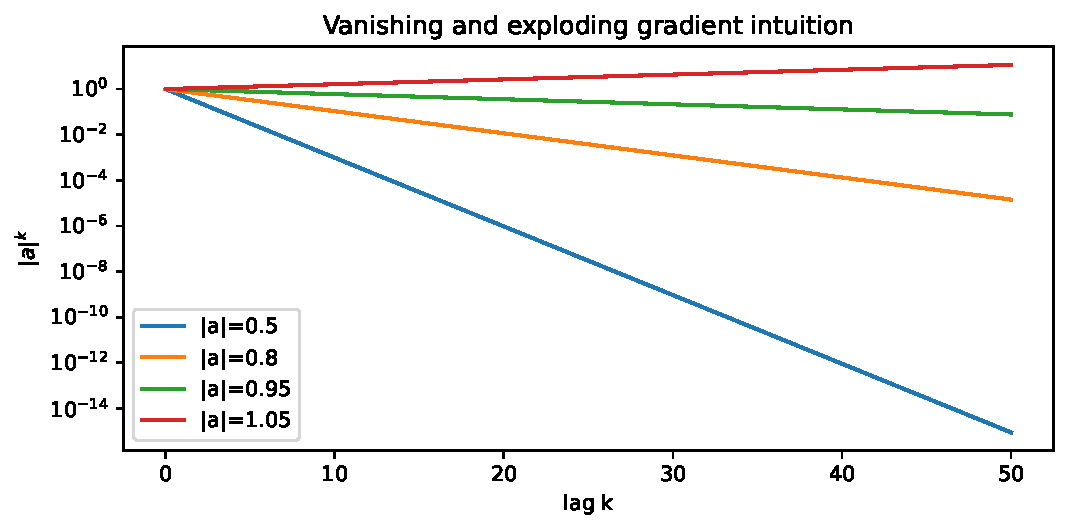
\includegraphics[keepaspectratio]{chapters/chapter-21-rnn-lstm-gru_files/figure-pdf/ch21-gradient-flow-output-1.pdf}}

}

\caption{Gradient factor a\^{}k for different recurrent weights.}

\end{figure}%

\section{21.15 Baselines and
diagnostics}\label{baselines-and-diagnostics}

A recurrent model should not be considered successful merely because it
trains. It should improve on baselines. Common baselines include:

\begin{itemize}
\tightlist
\item
  last-value forecast: \(\widehat Y_{t+h}=Y_t\);
\item
  seasonal naive forecast: \(\widehat Y_{t+h}=Y_{t+h-s}\);
\item
  linear autoregression or ridge regression on lag features;
\item
  convolutional or MLP window model.
\end{itemize}

For each model, inspect:

\[
\text{RMSE}_h=\bigg[\frac{1}{N}\sum_{i=1}^N(\widehat Y_{i,h}-Y_{i,h})^2\bigg]^{1/2},
\]

for each horizon \(h=1,\ldots,H\). Also inspect residuals over time. A
model may look good on average while failing during regime changes,
high-volatility intervals, or seasonal transitions.

\begin{Shaded}
\begin{Highlighting}[]
\CommentTok{\# last{-}value baseline for every horizon}
\NormalTok{last\_value }\OperatorTok{=}\NormalTok{ X\_test[:, }\OperatorTok{{-}}\DecValTok{1}\NormalTok{:]}
\NormalTok{naive\_pred }\OperatorTok{=}\NormalTok{ np.repeat(last\_value, H, axis}\OperatorTok{=}\DecValTok{1}\NormalTok{)}

\NormalTok{rnn\_rmse\_by\_h }\OperatorTok{=}\NormalTok{ np.sqrt(np.mean((pred }\OperatorTok{{-}}\NormalTok{ Y\_test) }\OperatorTok{**} \DecValTok{2}\NormalTok{, axis}\OperatorTok{=}\DecValTok{0}\NormalTok{))}
\NormalTok{naive\_rmse\_by\_h }\OperatorTok{=}\NormalTok{ np.sqrt(np.mean((naive\_pred }\OperatorTok{{-}}\NormalTok{ Y\_test) }\OperatorTok{**} \DecValTok{2}\NormalTok{, axis}\OperatorTok{=}\DecValTok{0}\NormalTok{))}

\ControlFlowTok{for}\NormalTok{ h }\KeywordTok{in} \BuiltInTok{range}\NormalTok{(H):}
    \BuiltInTok{print}\NormalTok{(}
        \SpecialStringTok{f"h=}\SpecialCharTok{\{}\NormalTok{h }\OperatorTok{+} \DecValTok{1}\SpecialCharTok{\}}\SpecialStringTok{: RNN RMSE=}\SpecialCharTok{\{}\NormalTok{rnn\_rmse\_by\_h[h]}\SpecialCharTok{:.3f\}}\SpecialStringTok{, "}
        \SpecialStringTok{f"last{-}value RMSE=}\SpecialCharTok{\{}\NormalTok{naive\_rmse\_by\_h[h]}\SpecialCharTok{:.3f\}}\SpecialStringTok{"}
\NormalTok{    )}

\NormalTok{plt.figure(figsize}\OperatorTok{=}\NormalTok{(}\DecValTok{7}\NormalTok{, }\FloatTok{3.5}\NormalTok{))}
\NormalTok{plt.plot(np.arange(}\DecValTok{1}\NormalTok{, H }\OperatorTok{+} \DecValTok{1}\NormalTok{), rnn\_rmse\_by\_h, marker}\OperatorTok{=}\StringTok{"o"}\NormalTok{, label}\OperatorTok{=}\StringTok{"RNN"}\NormalTok{)}
\NormalTok{plt.plot(np.arange(}\DecValTok{1}\NormalTok{, H }\OperatorTok{+} \DecValTok{1}\NormalTok{), naive\_rmse\_by\_h, marker}\OperatorTok{=}\StringTok{"o"}\NormalTok{, label}\OperatorTok{=}\StringTok{"last{-}value baseline"}\NormalTok{)}
\NormalTok{plt.xlabel(}\StringTok{"forecast horizon"}\NormalTok{)}
\NormalTok{plt.ylabel(}\StringTok{"RMSE"}\NormalTok{)}
\NormalTok{plt.title(}\StringTok{"Horizon{-}wise forecast error"}\NormalTok{)}
\NormalTok{plt.legend()}
\NormalTok{plt.show()}
\end{Highlighting}
\end{Shaded}

\begin{verbatim}
h=1: RNN RMSE=0.644, last-value RMSE=0.572
h=2: RNN RMSE=0.817, last-value RMSE=0.832
h=3: RNN RMSE=1.012, last-value RMSE=1.050
h=4: RNN RMSE=1.280, last-value RMSE=1.238
h=5: RNN RMSE=1.469, last-value RMSE=1.364
h=6: RNN RMSE=1.740, last-value RMSE=1.447
\end{verbatim}

\pandocbounded{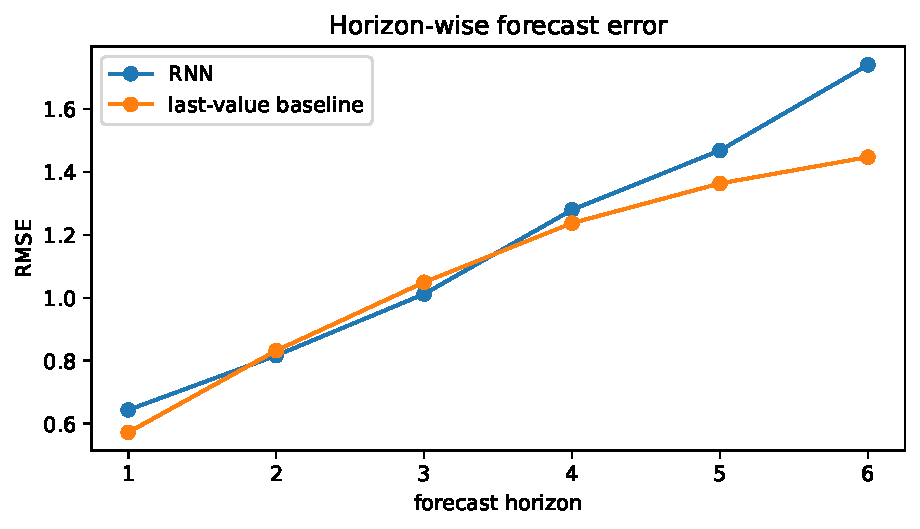
\includegraphics[keepaspectratio]{chapters/chapter-21-rnn-lstm-gru_files/figure-pdf/ch21-baseline-comparison-output-2.pdf}}

\section{21.16 AI-assisted modeling
activity}\label{ai-assisted-modeling-activity-4}

\section{AI-assisted code review
prompt}\label{ai-assisted-code-review-prompt}

Give an AI assistant your RNN, LSTM, or GRU training code and ask:

\begin{enumerate}
\def\labelenumi{\arabic{enumi}.}
\tightlist
\item
  Identify the tensor shapes at every major step.
\item
  Identify any possible data leakage.
\item
  Check whether scaling is fit only on the training set.
\item
  Check whether validation respects time order.
\item
  Explain whether the model predicts one step, multiple steps directly,
  or multiple steps recursively.
\item
  Suggest one baseline that must be included before claiming
  improvement.
\item
  Suggest one diagnostic plot for forecast errors.
\end{enumerate}

Then verify the answer by reading the code yourself. Do not accept a
model recommendation unless the validation design is correct.

\section{21.17 Common mistakes}\label{common-mistakes-20}

\begin{enumerate}
\def\labelenumi{\arabic{enumi}.}
\tightlist
\item
  \textbf{Randomly splitting windows.} Adjacent windows overlap heavily.
  A random split lets nearly identical histories appear in both training
  and test sets.
\item
  \textbf{Scaling on the full series.} This leaks future distributional
  information into the training set.
\item
  \textbf{Confusing hidden size with memory length.} A larger hidden
  dimension does not automatically solve long-range dependence.
\item
  \textbf{Using teacher forcing without deployment awareness.} If the
  model uses true previous future values during training, deployment
  performance may be worse.
\item
  \textbf{Not comparing with baselines.} RNNs often look impressive but
  may fail to beat seasonal naive, ARIMA, lag-feature regression, or TCN
  models.
\item
  \textbf{Ignoring tensor shapes.} Many recurrent model bugs are silent
  shape bugs.
\item
  \textbf{Overtraining small time series.} A recurrent network can
  memorize a short sequence without learning a robust forecasting rule.
\end{enumerate}

\section{21.18 Exercises}\label{exercises-20}

\begin{enumerate}
\def\labelenumi{\arabic{enumi}.}
\tightlist
\item
  For the scalar recurrence \(h_t=a h_{t-1}+b x_t\), derive \(h_t\) as a
  weighted sum of \(x_t,x_{t-1},\ldots,x_1\) and \(h_0\).
\item
  Show that \(\partial h_t/\partial h_{t-k}=a^k\) in the scalar linear
  case.
\item
  Explain why \(\tanh\) can reduce exploding states but does not
  completely solve vanishing gradients.
\item
  Write the LSTM equations and identify which gate controls memory
  retention.
\item
  Write the GRU equations and explain the update gate in words.
\item
  Build a direct \(H=12\) horizon GRU forecaster and compare it with a
  last-value baseline.
\item
  Repeat the experiment with an LSTM and report horizon-wise RMSE.
\item
  Create a sequence with a long delayed effect. Compare a vanilla RNN,
  LSTM, and TCN.
\item
  Ask an AI assistant to diagnose your model. List one suggestion that
  was correct and one suggestion that needed verification or correction.
\end{enumerate}

\section{21.19 Mini project}\label{mini-project-4}

Choose a univariate or multivariate time series. Build three models:

\begin{enumerate}
\def\labelenumi{\arabic{enumi}.}
\tightlist
\item
  a baseline model;
\item
  an LSTM or GRU model;
\item
  a non-recurrent model from an earlier chapter, such as ARIMA,
  lag-feature gradient boosting, or TCN.
\end{enumerate}

Your report should include:

\begin{itemize}
\tightlist
\item
  a description of the forecasting task and horizon;
\item
  the chronological split;
\item
  the scaling procedure;
\item
  tensor shapes for the recurrent model;
\item
  horizon-wise errors;
\item
  at least one forecast plot;
\item
  one diagnostic of failure cases;
\item
  a short AI-assisted code-review section explaining what was checked
  manually.
\end{itemize}

\section{21.20 Checklist}\label{checklist-5}

Before moving on, make sure you can answer the following questions.

\begin{itemize}
\tightlist
\item
  What does the hidden state represent?
\item
  Why are RNN weights shared across time?
\item
  What is backpropagation through time?
\item
  Why do products of Jacobians cause vanishing or exploding gradients?
\item
  What is the difference between an LSTM hidden state and cell state?
\item
  What do the forget, input, and output gates do?
\item
  What do the GRU update and reset gates do?
\item
  What tensor shape does PyTorch expect when \texttt{batch\_first=True}?
\item
  How do you avoid leakage when creating overlapping windows?
\item
  Which baseline must your recurrent model beat?
\end{itemize}

\chapter{Attention and Transformer Models for Time Series and Sequence
Data}\label{attention-and-transformer-models-for-time-series-and-sequence-data}

\textbf{Part VI. Deep Learning for Time Series and Sequence Data}\\
\textbf{Chapter goal:} understand self-attention and transformer models
as modern sequence-learning architectures. We study scaled dot-product
attention, causal masking, positional encoding, multi-head attention,
transformer blocks, forecasting architectures, Python implementation,
leakage-aware validation, and AI-assisted model critique.

\section{Learning objectives}\label{learning-objectives-21}

After studying this chapter, you should be able to:

\begin{enumerate}
\def\labelenumi{\arabic{enumi}.}
\tightlist
\item
  explain why attention was introduced as an alternative to
  fixed-window, convolutional, and recurrent sequence summaries;
\item
  compute scaled dot-product attention from query, key, and value
  matrices;
\item
  construct a causal mask for forecasting so that time \(t\) cannot use
  future values \(t+1,t+2,\ldots\);
\item
  describe sinusoidal and learned positional encodings and explain why a
  transformer needs position information;
\item
  derive the structure of a multi-head self-attention layer;
\item
  distinguish encoder-style and decoder-style transformer forecasting
  models;
\item
  implement a small transformer forecaster in PyTorch using
  chronological data splits;
\item
  diagnose common errors in transformer forecasting, including leakage,
  inappropriate masking, overparameterization, and poor baselines;
\item
  use AI tools to review attention-based sequence-model code while
  independently checking the mathematics and validation design.
\end{enumerate}

\section{22.1 Motivation: why
attention?}\label{motivation-why-attention}

The previous chapters considered several ways to summarize the past.

A feature-based model uses a fixed design vector such as

\[
\mathbf z_t=(y_t,y_{t-1},\ldots,y_{t-L+1},\text{calendar features},\text{covariates}).
\]

A convolutional model scans local filters over a window. A recurrent
model processes the sequence recursively through a hidden state

\[
\mathbf h_t = F_\Theta(\mathbf x_t,\mathbf h_{t-1}).
\]

These architectures are useful, but they impose a particular way to
compress history. In an RNN, information from the remote past must pass
through many recurrence steps. In a convolutional model, information is
organized by local receptive fields. Attention takes another viewpoint:
for each time point, the model learns which other time points should be
used directly.

The central operation is a weighted average. For a query time \(t\),
attention produces weights

\[
\alpha_{t,s}\geq 0,
\qquad
\sum_s \alpha_{t,s}=1,
\]

and forms a context vector

\[
\mathbf c_t=\sum_s \alpha_{t,s}\mathbf v_s.
\]

Here \(\mathbf v_s\) is a value vector associated with time \(s\). The
weights are not fixed. They depend on the data through learned query and
key vectors.

\begin{tcolorbox}[enhanced jigsaw, arc=.35mm, bottomrule=.15mm, bottomtitle=1mm, breakable, colback=white, colbacktitle=quarto-callout-note-color!10!white, colframe=quarto-callout-note-color-frame, coltitle=black, left=2mm, leftrule=.75mm, opacityback=0, opacitybacktitle=0.6, rightrule=.15mm, title=\textcolor{quarto-callout-note-color}{\faInfo}\hspace{0.5em}{Forecasting intuition}, titlerule=0mm, toprule=.15mm, toptitle=1mm]

For forecasting, attention can learn patterns such as: ``the current
value should look at yesterday,'' ``the current value should look at the
same hour last week,'' or ``the current value should look at the most
recent shock.'' Causal attention enforces that a prediction made at time
\(t\) cannot use information from times greater than \(t\).

\end{tcolorbox}

\section{22.2 Tokens, embeddings, queries, keys, and
values}\label{tokens-embeddings-queries-keys-and-values}

Suppose a sequence has length \(T\) and each observation is represented
by

\[
\mathbf x_t\in\mathbb R^{d_x},
\qquad t=1,\ldots,T.
\]

A transformer first maps each observation to a model-dimensional vector

\[
\mathbf e_t = E_\Theta(\mathbf x_t)\in\mathbb R^{d_{\text{model}}}.
\]

For a univariate time series, this embedding could be a linear
projection

\[
\mathbf e_t=W_e y_t+\mathbf b_e,
\]

where \(W_e\in\mathbb R^{d_{\text{model}}\times 1}\). For multivariate
time series, the input may include past targets, exogenous variables,
static features, calendar features, and missingness indicators.

Self-attention constructs three matrices:

\[
Q = X W_Q,
\qquad
K = X W_K,
\qquad
V = X W_V,
\]

where

\[
X=\begin{bmatrix}
\mathbf e_1^T\\
\mathbf e_2^T\\
\vdots\\
\mathbf e_T^T
\end{bmatrix}\in\mathbb R^{T\times d_{\text{model}}}.
\]

The rows of \(Q,K,V\) are query, key, and value vectors:

\[
\mathbf q_t,
\quad
\mathbf k_t,
\quad
\mathbf v_t.
\]

The score between query time \(t\) and key time \(s\) is the dot product

\[
\operatorname{score}(t,s)=\mathbf q_t^T\mathbf k_s.
\]

Large positive scores mean that time \(t\) finds time \(s\) relevant.
Large negative scores mean that time \(s\) is suppressed.

\section{22.3 Scaled dot-product
attention}\label{scaled-dot-product-attention}

The basic attention map is

\[
\operatorname{Attention}(Q,K,V)
=
\operatorname{softmax}\left(\frac{QK^T}{\sqrt{d_k}}\right)V,
\]

where \(d_k\) is the key dimension. The score matrix is

\[
S=\frac{QK^T}{\sqrt{d_k}}\in\mathbb R^{T\times T}.
\]

For each query time \(t\), row \(t\) of \(S\) is converted to a
probability vector by the softmax function:

\[
\alpha_{t,s}
=
\frac{\exp(S_{t,s})}{\sum_{r=1}^T \exp(S_{t,r})}.
\]

The output at time \(t\) is

\[
\mathbf c_t
=
\sum_{s=1}^T \alpha_{t,s}\mathbf v_s.
\]

The division by \(\sqrt{d_k}\) stabilizes the scale of the dot products.
If the components of \(\mathbf q_t\) and \(\mathbf k_s\) have roughly
unit variance and are weakly dependent, then the dot product has
variance proportional to \(d_k\). Scaling keeps the softmax from
saturating too early.

\begin{tcolorbox}[enhanced jigsaw, arc=.35mm, bottomrule=.15mm, bottomtitle=1mm, breakable, colback=white, colbacktitle=quarto-callout-warning-color!10!white, colframe=quarto-callout-warning-color-frame, coltitle=black, left=2mm, leftrule=.75mm, opacityback=0, opacitybacktitle=0.6, rightrule=.15mm, title=\textcolor{quarto-callout-warning-color}{\faExclamationTriangle}\hspace{0.5em}{Numerical stability}, titlerule=0mm, toprule=.15mm, toptitle=1mm]

In code, softmax should be computed after subtracting the row maximum:

\[
\operatorname{softmax}(\mathbf z)_j
=\frac{\exp(z_j-\max_k z_k)}{\sum_r \exp(z_r-\max_k z_k)}.
\]

This does not change the result but prevents overflow.

\end{tcolorbox}

\section{22.4 Causal masking for
forecasting}\label{causal-masking-for-forecasting}

For sequence forecasting, the model must not look into the future. A
causal attention layer uses the mask

\[
M_{t,s}=\begin{cases}
0, & s\leq t,\\
-\infty, & s>t.
\end{cases}
\]

The causal attention weights are

\[
\alpha_{t,s}
=
\operatorname{softmax}\left(\frac{\mathbf q_t^T\mathbf k_s}{\sqrt{d_k}}+M_{t,s}\right).
\]

Therefore,

\[
\alpha_{t,s}=0
\qquad
\text{whenever }s>t.
\]

This is the mathematical mechanism behind autoregressive transformers.
The model may attend to the past and present, but not the future.

\begin{tcolorbox}[enhanced jigsaw, arc=.35mm, bottomrule=.15mm, bottomtitle=1mm, breakable, colback=white, colbacktitle=quarto-callout-important-color!10!white, colframe=quarto-callout-important-color-frame, coltitle=black, left=2mm, leftrule=.75mm, opacityback=0, opacitybacktitle=0.6, rightrule=.15mm, title=\textcolor{quarto-callout-important-color}{\faExclamation}\hspace{0.5em}{Leakage check}, titlerule=0mm, toprule=.15mm, toptitle=1mm]

A model can have excellent validation error for the wrong reason if
masking is incorrect. For one-step-ahead forecasting, the input
available at time \(t\) should contain information known at or before
time \(t\). The label \(y_{t+1}\) must not be included in the input
features or attention keys.

\end{tcolorbox}

\section{22.5 Interactive module: causal attention
heatmap}\label{interactive-module-causal-attention-heatmap}

This module constructs a deterministic sequence and an attention matrix.
The control parameters are not learned; they are used to visualize how
causal masking, temperature, and locality affect attention. The selected
query row shows which past times the model uses to form the context
value.

Interactive Module 22.1: Causal Self-Attention Heatmap

Change the sequence length, selected query time, temperature, locality
decay, and mask type. The future should receive zero attention under the
causal mask.

\begin{verbatim}
<label>Sequence length $T$
  <input id="ch22_attn_len" type="range" min="8" max="40" step="1" value="24">
  <span id="ch22_attn_len_value">24</span>
</label>

<label>Selected query time $t$
  <input id="ch22_attn_query" type="range" min="1" max="24" step="1" value="16">
  <span id="ch22_attn_query_value">16</span>
</label>

<label>Temperature $\tau$
  <input id="ch22_attn_temperature" type="range" min="0.25" max="3" step="0.05" value="1.00">
  <span id="ch22_attn_temperature_value">1.00</span>
</label>

<label>Locality decay
  <input id="ch22_attn_decay" type="range" min="2" max="20" step="1" value="7">
  <span id="ch22_attn_decay_value">7</span>
</label>

<label>Mask
  <select id="ch22_attn_mask">
    <option value="causal" selected>causal forecasting mask</option>
    <option value="none">no mask</option>
  </select>
</label>
\end{verbatim}

\protect\phantomsection\label{ch22_attention_heatmap}

\protect\phantomsection\label{ch22_attention_weights}

\section{22.6 Positional information}\label{positional-information}

Self-attention by itself is permutation-equivariant. If the input tokens
are rearranged, attention rearranges with them. But time series and
language are ordered. Therefore a transformer needs position
information.

One classical choice is sinusoidal positional encoding. For position
\(t\) and dimension \(j\), define

\[
\operatorname{PE}(t,2j)=\sin\left(\frac{t}{10000^{2j/d_{\text{model}}}}\right),
\]

\[
\operatorname{PE}(t,2j+1)=\cos\left(\frac{t}{10000^{2j/d_{\text{model}}}}\right).
\]

The input to attention becomes

\[
\widetilde{\mathbf e}_t=\mathbf e_t+\operatorname{PE}(t).
\]

The low-index positional components vary rapidly, and the high-index
components vary slowly. Together, they provide a multi-scale
representation of position.

Other common choices include learned positional embeddings, relative
position biases, rotary position embeddings, and time-feature
embeddings. For time series, calendar features such as hour of day, day
of week, month, holiday indicator, or age of observation are also
common.

\section{22.7 Interactive module: sinusoidal positional
encoding}\label{interactive-module-sinusoidal-positional-encoding}

This module visualizes sinusoidal positional features and their
similarity to a reference position. The similarity curve helps explain
why positional encodings give attention a notion of distance and order.

Interactive Module 22.2: Positional Encoding Explorer

Change the model dimension, reference position, and component index. The
lower components oscillate faster; higher components vary more slowly.

\begin{verbatim}
<label>Sequence length
  <input id="ch22_pos_len" type="range" min="24" max="160" step="4" value="80">
  <span id="ch22_pos_len_value">80</span>
</label>

<label>Model dimension $d_{\text{model}}$
  <select id="ch22_pos_dim">
    <option value="8">8</option>
    <option value="16" selected>16</option>
    <option value="32">32</option>
  </select>
</label>

<label>Reference position
  <input id="ch22_pos_ref" type="range" min="0" max="79" step="1" value="30">
  <span id="ch22_pos_ref_value">30</span>
</label>

<label>Component pair $j$
  <input id="ch22_pos_freq" type="range" min="0" max="7" step="1" value="2">
  <span id="ch22_pos_freq_value">2</span>
</label>
\end{verbatim}

\protect\phantomsection\label{ch22_pos_signal}

\protect\phantomsection\label{ch22_pos_similarity}

\section{22.8 Multi-head attention}\label{multi-head-attention}

A single attention head computes one representation of relevance.
Multi-head attention computes several attention maps in parallel:

\[
\operatorname{head}_h
=
\operatorname{Attention}(QW_Q^{(h)},KW_K^{(h)},VW_V^{(h)}),
\]

for \(h=1,\ldots,H\). The heads are concatenated and projected:

\[
\operatorname{MHA}(Q,K,V)
=
\operatorname{Concat}(\operatorname{head}_1,\ldots,\operatorname{head}_H)W_O.
\]

Different heads can specialize in different structures: short-lag
dependence, seasonal lag dependence, event response, local smoothing, or
long-range similarity. In practice, these interpretations are suggestive
rather than guaranteed. Attention weights are useful diagnostics, but
they are not always faithful explanations of the model's decision.

\section{22.9 Transformer block}\label{transformer-block}

A standard transformer block contains two main sublayers:

\begin{enumerate}
\def\labelenumi{\arabic{enumi}.}
\tightlist
\item
  multi-head self-attention;
\item
  a position-wise feedforward network.
\end{enumerate}

With residual connections and layer normalization, one common schematic
is

\[
Z^{(1)}=\operatorname{LayerNorm}(X+\operatorname{MHA}(X,X,X)),
\]

\[
Z^{(2)}=\operatorname{LayerNorm}(Z^{(1)}+\operatorname{FFN}(Z^{(1)})).
\]

The feedforward network is applied independently at every time step:

\[
\operatorname{FFN}(\mathbf z)
=W_2\sigma(W_1\mathbf z+\mathbf b_1)+\mathbf b_2.
\]

The residual path helps optimization. Layer normalization stabilizes
scale. Dropout regularizes the model.

\section{22.10 Forecasting
architectures}\label{forecasting-architectures-1}

There are several ways to use transformers for time-series forecasting.

\textbf{Encoder-style window forecasting.} Given an input window

\[
y_{t-L+1},\ldots,y_t,
\]

the model encodes the window and predicts

\[
\widehat{\mathbf y}_{t+1:t+H}
=
(\widehat y_{t+1},\ldots,\widehat y_{t+H}).
\]

This is similar to the MLP, CNN, and RNN window workflows, but the
encoder block is attention-based.

\textbf{Autoregressive decoder forecasting.} The model predicts one
token at a time using a causal mask. For a sequence model,

\[
p(y_{1:T})=\prod_{t=1}^T p(y_t\mid y_{1:t-1}).
\]

This is the same factorization used by autoregressive language models.
For time series, the output distribution may be Gaussian, Student-\(t\),
negative binomial, quantile-based, or another task-appropriate
distribution.

\textbf{Encoder-decoder forecasting.} An encoder summarizes historical
context, and a decoder generates the forecast horizon. This is useful
when future-known covariates such as calendar features, planned prices,
or weather forecasts are available.

\begin{tcolorbox}[enhanced jigsaw, arc=.35mm, bottomrule=.15mm, bottomtitle=1mm, breakable, colback=white, colbacktitle=quarto-callout-tip-color!10!white, colframe=quarto-callout-tip-color-frame, coltitle=black, left=2mm, leftrule=.75mm, opacityback=0, opacitybacktitle=0.6, rightrule=.15mm, title=\textcolor{quarto-callout-tip-color}{\faLightbulb}\hspace{0.5em}{Practical recommendation}, titlerule=0mm, toprule=.15mm, toptitle=1mm]

For an applied forecasting project, begin with naive, seasonal naive,
ARIMA/SARIMA, and feature-based baselines. Then compare a small
transformer against these baselines using rolling-origin validation. A
transformer that beats a random split but not a seasonal naive baseline
is not useful.

\end{tcolorbox}

\section{22.11 Computational cost and long
sequences}\label{computational-cost-and-long-sequences}

Full self-attention stores a \(T\times T\) score matrix. Therefore the
memory and time cost scale roughly as

\[
O(T^2 d_{\text{model}}).
\]

This is expensive for long time series. Several strategies reduce the
cost:

\begin{itemize}
\tightlist
\item
  downsample or patch the sequence;
\item
  use local attention windows;
\item
  use sparse attention patterns;
\item
  use low-rank or kernel approximations;
\item
  combine attention with convolution or state-space layers;
\item
  use hierarchical representations.
\end{itemize}

The right choice depends on the data frequency, forecast horizon,
latency constraints, and whether the model needs very long context.

\section{22.12 Python example: scaled dot-product attention from
scratch}\label{python-example-scaled-dot-product-attention-from-scratch}

The following code implements causal scaled dot-product attention using
only NumPy. Notice how the future weights become zero after masking.

\begin{Shaded}
\begin{Highlighting}[]
\ImportTok{import}\NormalTok{ numpy }\ImportTok{as}\NormalTok{ np}
\ImportTok{import}\NormalTok{ matplotlib.pyplot }\ImportTok{as}\NormalTok{ plt}

\NormalTok{rng }\OperatorTok{=}\NormalTok{ np.random.default\_rng(}\DecValTok{22}\NormalTok{)}
\NormalTok{T }\OperatorTok{=} \DecValTok{12}
\NormalTok{D }\OperatorTok{=} \DecValTok{6}

\CommentTok{\# Synthetic embedded sequence.}
\NormalTok{t }\OperatorTok{=}\NormalTok{ np.arange(T)}
\NormalTok{X\_embed }\OperatorTok{=}\NormalTok{ np.column\_stack([}
\NormalTok{    np.sin(}\DecValTok{2} \OperatorTok{*}\NormalTok{ np.pi }\OperatorTok{*}\NormalTok{ t }\OperatorTok{/} \DecValTok{6}\NormalTok{),}
\NormalTok{    np.cos(}\DecValTok{2} \OperatorTok{*}\NormalTok{ np.pi }\OperatorTok{*}\NormalTok{ t }\OperatorTok{/} \DecValTok{6}\NormalTok{),}
\NormalTok{    t }\OperatorTok{/}\NormalTok{ T,}
\NormalTok{    (t }\OperatorTok{\textgreater{}=} \DecValTok{7}\NormalTok{).astype(}\BuiltInTok{float}\NormalTok{),}
\NormalTok{    rng.normal(scale}\OperatorTok{=}\FloatTok{0.1}\NormalTok{, size}\OperatorTok{=}\NormalTok{T),}
\NormalTok{    np.ones(T),}
\NormalTok{])}

\NormalTok{Wq }\OperatorTok{=}\NormalTok{ rng.normal(scale}\OperatorTok{=}\FloatTok{0.4}\NormalTok{, size}\OperatorTok{=}\NormalTok{(D, D))}
\NormalTok{Wk }\OperatorTok{=}\NormalTok{ rng.normal(scale}\OperatorTok{=}\FloatTok{0.4}\NormalTok{, size}\OperatorTok{=}\NormalTok{(D, D))}
\NormalTok{Wv }\OperatorTok{=}\NormalTok{ rng.normal(scale}\OperatorTok{=}\FloatTok{0.4}\NormalTok{, size}\OperatorTok{=}\NormalTok{(D, D))}

\NormalTok{Q }\OperatorTok{=}\NormalTok{ X\_embed }\OperatorTok{@}\NormalTok{ Wq}
\NormalTok{K }\OperatorTok{=}\NormalTok{ X\_embed }\OperatorTok{@}\NormalTok{ Wk}
\NormalTok{V }\OperatorTok{=}\NormalTok{ X\_embed }\OperatorTok{@}\NormalTok{ Wv}

\NormalTok{scores }\OperatorTok{=}\NormalTok{ Q }\OperatorTok{@}\NormalTok{ K.T }\OperatorTok{/}\NormalTok{ np.sqrt(D)}
\NormalTok{causal\_mask }\OperatorTok{=}\NormalTok{ np.triu(np.ones((T, T), dtype}\OperatorTok{=}\BuiltInTok{bool}\NormalTok{), k}\OperatorTok{=}\DecValTok{1}\NormalTok{)}
\NormalTok{scores\_masked }\OperatorTok{=}\NormalTok{ scores.copy()}
\NormalTok{scores\_masked[causal\_mask] }\OperatorTok{=} \OperatorTok{{-}}\FloatTok{1e9}

\KeywordTok{def}\NormalTok{ row\_softmax(A):}
\NormalTok{    B }\OperatorTok{=}\NormalTok{ A }\OperatorTok{{-}}\NormalTok{ A.}\BuiltInTok{max}\NormalTok{(axis}\OperatorTok{=}\DecValTok{1}\NormalTok{, keepdims}\OperatorTok{=}\VariableTok{True}\NormalTok{)}
\NormalTok{    E }\OperatorTok{=}\NormalTok{ np.exp(B)}
    \ControlFlowTok{return}\NormalTok{ E }\OperatorTok{/}\NormalTok{ E.}\BuiltInTok{sum}\NormalTok{(axis}\OperatorTok{=}\DecValTok{1}\NormalTok{, keepdims}\OperatorTok{=}\VariableTok{True}\NormalTok{)}

\NormalTok{A }\OperatorTok{=}\NormalTok{ row\_softmax(scores\_masked)}
\NormalTok{C }\OperatorTok{=}\NormalTok{ A }\OperatorTok{@}\NormalTok{ V}

\BuiltInTok{print}\NormalTok{(}\StringTok{"Attention shape:"}\NormalTok{, A.shape)}
\BuiltInTok{print}\NormalTok{(}\StringTok{"Context shape:"}\NormalTok{, C.shape)}
\BuiltInTok{print}\NormalTok{(}\StringTok{"Largest future attention weight:"}\NormalTok{, A[causal\_mask].}\BuiltInTok{max}\NormalTok{())}

\NormalTok{plt.figure(figsize}\OperatorTok{=}\NormalTok{(}\DecValTok{6}\NormalTok{, }\FloatTok{4.8}\NormalTok{))}
\NormalTok{plt.imshow(A, aspect}\OperatorTok{=}\StringTok{"auto"}\NormalTok{, origin}\OperatorTok{=}\StringTok{"lower"}\NormalTok{)}
\NormalTok{plt.colorbar(label}\OperatorTok{=}\StringTok{"attention weight"}\NormalTok{)}
\NormalTok{plt.xlabel(}\StringTok{"key time"}\NormalTok{)}
\NormalTok{plt.ylabel(}\StringTok{"query time"}\NormalTok{)}
\NormalTok{plt.title(}\StringTok{"Causal self{-}attention weights"}\NormalTok{)}
\NormalTok{plt.show()}
\end{Highlighting}
\end{Shaded}

\begin{verbatim}
Attention shape: (12, 12)
Context shape: (12, 6)
Largest future attention weight: 0.0
\end{verbatim}

\begin{figure}[H]

{\centering \pandocbounded{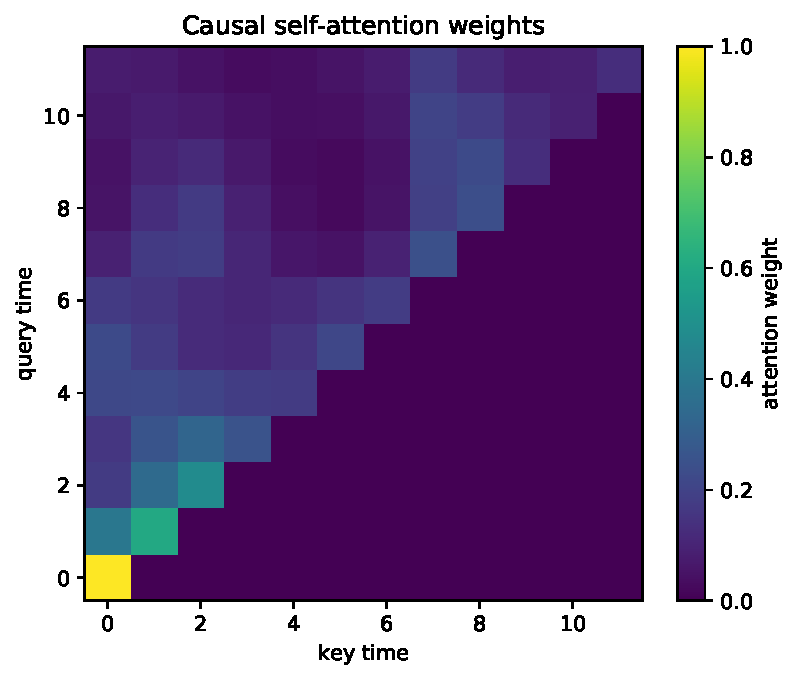
\includegraphics[keepaspectratio]{chapters/chapter-22-attention-transformers-time-series_files/figure-pdf/ch22-scaled-dot-product-attention-output-2.pdf}}

}

\caption{Causal self-attention matrix computed from scratch.}

\end{figure}%

\section{22.13 Python example: positional
encoding}\label{python-example-positional-encoding}

The next example constructs sinusoidal positional encodings and plots
two components.

\begin{Shaded}
\begin{Highlighting}[]
\KeywordTok{def}\NormalTok{ sinusoidal\_positional\_encoding(length, d\_model):}
\NormalTok{    positions }\OperatorTok{=}\NormalTok{ np.arange(length)[:, }\VariableTok{None}\NormalTok{]}
\NormalTok{    dims }\OperatorTok{=}\NormalTok{ np.arange(d\_model)[}\VariableTok{None}\NormalTok{, :]}
\NormalTok{    angle\_rates }\OperatorTok{=} \DecValTok{1} \OperatorTok{/}\NormalTok{ np.power(}\DecValTok{10000}\NormalTok{, (}\DecValTok{2} \OperatorTok{*}\NormalTok{ (dims }\OperatorTok{//} \DecValTok{2}\NormalTok{)) }\OperatorTok{/}\NormalTok{ d\_model)}
\NormalTok{    angles }\OperatorTok{=}\NormalTok{ positions }\OperatorTok{*}\NormalTok{ angle\_rates}
\NormalTok{    pe }\OperatorTok{=}\NormalTok{ np.zeros((length, d\_model))}
\NormalTok{    pe[:, }\DecValTok{0}\NormalTok{::}\DecValTok{2}\NormalTok{] }\OperatorTok{=}\NormalTok{ np.sin(angles[:, }\DecValTok{0}\NormalTok{::}\DecValTok{2}\NormalTok{])}
\NormalTok{    pe[:, }\DecValTok{1}\NormalTok{::}\DecValTok{2}\NormalTok{] }\OperatorTok{=}\NormalTok{ np.cos(angles[:, }\DecValTok{1}\NormalTok{::}\DecValTok{2}\NormalTok{])}
    \ControlFlowTok{return}\NormalTok{ pe}

\NormalTok{L }\OperatorTok{=} \DecValTok{100}
\NormalTok{d\_model }\OperatorTok{=} \DecValTok{16}
\NormalTok{pe }\OperatorTok{=}\NormalTok{ sinusoidal\_positional\_encoding(L, d\_model)}

\NormalTok{plt.figure(figsize}\OperatorTok{=}\NormalTok{(}\DecValTok{8}\NormalTok{, }\FloatTok{3.5}\NormalTok{))}
\NormalTok{plt.plot(pe[:, }\DecValTok{0}\NormalTok{], label}\OperatorTok{=}\StringTok{"PE dimension 0"}\NormalTok{)}
\NormalTok{plt.plot(pe[:, }\DecValTok{1}\NormalTok{], label}\OperatorTok{=}\StringTok{"PE dimension 1"}\NormalTok{)}
\NormalTok{plt.plot(pe[:, }\DecValTok{6}\NormalTok{], label}\OperatorTok{=}\StringTok{"PE dimension 6"}\NormalTok{)}
\NormalTok{plt.xlabel(}\StringTok{"position"}\NormalTok{)}
\NormalTok{plt.ylabel(}\StringTok{"encoding value"}\NormalTok{)}
\NormalTok{plt.title(}\StringTok{"Sinusoidal positional encoding"}\NormalTok{)}
\NormalTok{plt.legend()}
\NormalTok{plt.show()}

\NormalTok{ref }\OperatorTok{=} \DecValTok{30}
\NormalTok{similarity }\OperatorTok{=}\NormalTok{ pe }\OperatorTok{@}\NormalTok{ pe[ref] }\OperatorTok{/}\NormalTok{ np.sqrt(d\_model)}
\BuiltInTok{print}\NormalTok{(}\StringTok{"Most similar positions to reference, excluding itself:"}\NormalTok{)}
\NormalTok{order }\OperatorTok{=}\NormalTok{ np.argsort(}\OperatorTok{{-}}\NormalTok{similarity)}
\BuiltInTok{print}\NormalTok{([}\BuiltInTok{int}\NormalTok{(i) }\ControlFlowTok{for}\NormalTok{ i }\KeywordTok{in}\NormalTok{ order }\ControlFlowTok{if}\NormalTok{ i }\OperatorTok{!=}\NormalTok{ ref][:}\DecValTok{5}\NormalTok{])}
\end{Highlighting}
\end{Shaded}

\begin{figure}[H]

{\centering \pandocbounded{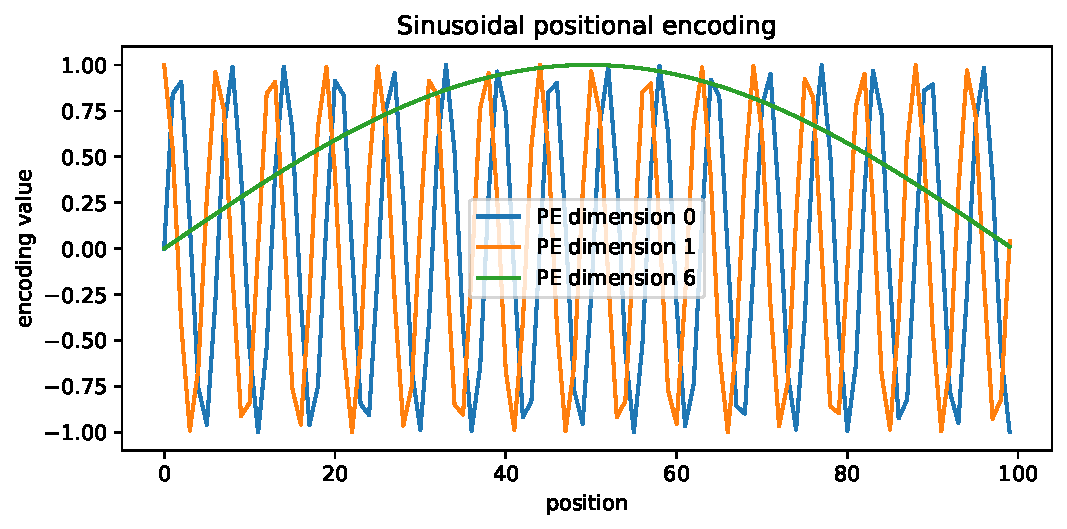
\includegraphics[keepaspectratio]{chapters/chapter-22-attention-transformers-time-series_files/figure-pdf/ch22-positional-encoding-output-1.pdf}}

}

\caption{Selected sinusoidal positional encoding components.}

\end{figure}%

\begin{verbatim}
Most similar positions to reference, excluding itself:
[29, 31, 24, 36, 11]
\end{verbatim}

\section{22.14 Python example: PyTorch multi-head
attention}\label{python-example-pytorch-multi-head-attention}

PyTorch includes a multi-head attention layer. The example below uses a
causal mask. The mask has shape \(T\times T\) and is \texttt{True}
exactly where attention is not allowed.

\protect\phantomsection\label{ch22-pytorch-multihead-attention}
\begin{Shaded}
\begin{Highlighting}[]
\ImportTok{import}\NormalTok{ torch}
\ImportTok{import}\NormalTok{ torch.nn }\ImportTok{as}\NormalTok{ nn}

\NormalTok{torch.set\_num\_threads(}\DecValTok{1}\NormalTok{)}
\NormalTok{torch.manual\_seed(}\DecValTok{22}\NormalTok{)}
\NormalTok{B }\OperatorTok{=} \DecValTok{3}       \CommentTok{\# batch size}
\NormalTok{T }\OperatorTok{=} \DecValTok{10}      \CommentTok{\# sequence length}
\NormalTok{d\_model }\OperatorTok{=} \DecValTok{16}
\NormalTok{n\_heads }\OperatorTok{=} \DecValTok{4}

\NormalTok{x }\OperatorTok{=}\NormalTok{ torch.randn(B, T, d\_model)}
\NormalTok{attn }\OperatorTok{=}\NormalTok{ nn.MultiheadAttention(}
\NormalTok{    embed\_dim}\OperatorTok{=}\NormalTok{d\_model,}
\NormalTok{    num\_heads}\OperatorTok{=}\NormalTok{n\_heads,}
\NormalTok{    batch\_first}\OperatorTok{=}\VariableTok{True}\NormalTok{,}
\NormalTok{)}

\NormalTok{causal\_mask }\OperatorTok{=}\NormalTok{ torch.triu(torch.ones(T, T, dtype}\OperatorTok{=}\NormalTok{torch.}\BuiltInTok{bool}\NormalTok{), diagonal}\OperatorTok{=}\DecValTok{1}\NormalTok{)}
\NormalTok{out, weights }\OperatorTok{=}\NormalTok{ attn(x, x, x, attn\_mask}\OperatorTok{=}\NormalTok{causal\_mask, need\_weights}\OperatorTok{=}\VariableTok{True}\NormalTok{)}

\BuiltInTok{print}\NormalTok{(}\StringTok{"input shape:"}\NormalTok{, }\BuiltInTok{tuple}\NormalTok{(x.shape))}
\BuiltInTok{print}\NormalTok{(}\StringTok{"output shape:"}\NormalTok{, }\BuiltInTok{tuple}\NormalTok{(out.shape))}
\BuiltInTok{print}\NormalTok{(}\StringTok{"attention weight shape:"}\NormalTok{, }\BuiltInTok{tuple}\NormalTok{(weights.shape))}
\BuiltInTok{print}\NormalTok{(}\StringTok{"mask true means future positions are hidden:"}\NormalTok{)}
\BuiltInTok{print}\NormalTok{(causal\_mask.}\BuiltInTok{int}\NormalTok{())}
\end{Highlighting}
\end{Shaded}

\begin{verbatim}
input shape: (3, 10, 16)
output shape: (3, 10, 16)
attention weight shape: (3, 10, 10)
mask true means future positions are hidden:
tensor([[0, 1, 1, 1, 1, 1, 1, 1, 1, 1],
        [0, 0, 1, 1, 1, 1, 1, 1, 1, 1],
        [0, 0, 0, 1, 1, 1, 1, 1, 1, 1],
        [0, 0, 0, 0, 1, 1, 1, 1, 1, 1],
        [0, 0, 0, 0, 0, 1, 1, 1, 1, 1],
        [0, 0, 0, 0, 0, 0, 1, 1, 1, 1],
        [0, 0, 0, 0, 0, 0, 0, 1, 1, 1],
        [0, 0, 0, 0, 0, 0, 0, 0, 1, 1],
        [0, 0, 0, 0, 0, 0, 0, 0, 0, 1],
        [0, 0, 0, 0, 0, 0, 0, 0, 0, 0]], dtype=torch.int32)
\end{verbatim}

\section{22.15 Python example: a small transformer
forecaster}\label{python-example-a-small-transformer-forecaster}

Now we build a small encoder-style transformer forecaster. The model
receives a window of length \(L\) and predicts the next \(H\) values.
This example is intentionally small so that the code emphasizes
structure rather than performance.

\begin{Shaded}
\begin{Highlighting}[]
\ImportTok{from}\NormalTok{ sklearn.preprocessing }\ImportTok{import}\NormalTok{ StandardScaler}

\NormalTok{rng }\OperatorTok{=}\NormalTok{ np.random.default\_rng(}\DecValTok{222}\NormalTok{)}
\NormalTok{T\_total }\OperatorTok{=} \DecValTok{520}
\NormalTok{t }\OperatorTok{=}\NormalTok{ np.arange(T\_total)}

\NormalTok{y }\OperatorTok{=}\NormalTok{ (}
    \FloatTok{0.006} \OperatorTok{*}\NormalTok{ t}
    \OperatorTok{+} \FloatTok{1.2} \OperatorTok{*}\NormalTok{ np.sin(}\DecValTok{2} \OperatorTok{*}\NormalTok{ np.pi }\OperatorTok{*}\NormalTok{ t }\OperatorTok{/} \DecValTok{24}\NormalTok{)}
    \OperatorTok{+} \FloatTok{0.55} \OperatorTok{*}\NormalTok{ np.sin(}\DecValTok{2} \OperatorTok{*}\NormalTok{ np.pi }\OperatorTok{*}\NormalTok{ t }\OperatorTok{/} \DecValTok{7}\NormalTok{)}
    \OperatorTok{+} \FloatTok{0.9} \OperatorTok{*}\NormalTok{ (t }\OperatorTok{\textgreater{}=} \DecValTok{320}\NormalTok{)}
    \OperatorTok{+}\NormalTok{ rng.normal(scale}\OperatorTok{=}\FloatTok{0.25}\NormalTok{, size}\OperatorTok{=}\NormalTok{T\_total)}
\NormalTok{)}

\NormalTok{L }\OperatorTok{=} \DecValTok{36}
\NormalTok{H }\OperatorTok{=} \DecValTok{6}
\NormalTok{X\_windows, Y\_windows, origins }\OperatorTok{=}\NormalTok{ [], [], []}
\ControlFlowTok{for}\NormalTok{ start }\KeywordTok{in} \BuiltInTok{range}\NormalTok{(T\_total }\OperatorTok{{-}}\NormalTok{ L }\OperatorTok{{-}}\NormalTok{ H }\OperatorTok{+} \DecValTok{1}\NormalTok{):}
\NormalTok{    X\_windows.append(y[start:start }\OperatorTok{+}\NormalTok{ L])}
\NormalTok{    Y\_windows.append(y[start }\OperatorTok{+}\NormalTok{ L:start }\OperatorTok{+}\NormalTok{ L }\OperatorTok{+}\NormalTok{ H])}
\NormalTok{    origins.append(start }\OperatorTok{+}\NormalTok{ L }\OperatorTok{{-}} \DecValTok{1}\NormalTok{)}

\NormalTok{X\_windows }\OperatorTok{=}\NormalTok{ np.asarray(X\_windows)}
\NormalTok{Y\_windows }\OperatorTok{=}\NormalTok{ np.asarray(Y\_windows)}
\NormalTok{origins }\OperatorTok{=}\NormalTok{ np.asarray(origins)}

\NormalTok{train\_mask }\OperatorTok{=}\NormalTok{ origins }\OperatorTok{\textless{}} \DecValTok{360}
\NormalTok{test\_mask }\OperatorTok{=}\NormalTok{ origins }\OperatorTok{\textgreater{}=} \DecValTok{360}

\NormalTok{x\_scaler }\OperatorTok{=}\NormalTok{ StandardScaler()}
\NormalTok{y\_scaler }\OperatorTok{=}\NormalTok{ StandardScaler()}

\NormalTok{X\_train }\OperatorTok{=}\NormalTok{ x\_scaler.fit\_transform(X\_windows[train\_mask])}
\NormalTok{X\_test }\OperatorTok{=}\NormalTok{ x\_scaler.transform(X\_windows[test\_mask])}
\NormalTok{Y\_train }\OperatorTok{=}\NormalTok{ y\_scaler.fit\_transform(Y\_windows[train\_mask])}
\NormalTok{Y\_test }\OperatorTok{=}\NormalTok{ y\_scaler.transform(Y\_windows[test\_mask])}

\NormalTok{plt.figure(figsize}\OperatorTok{=}\NormalTok{(}\DecValTok{8}\NormalTok{, }\FloatTok{3.5}\NormalTok{))}
\NormalTok{plt.plot(t, y, label}\OperatorTok{=}\StringTok{"observed"}\NormalTok{)}
\NormalTok{plt.axvline(}\DecValTok{360}\NormalTok{, linestyle}\OperatorTok{=}\StringTok{"{-}{-}"}\NormalTok{, label}\OperatorTok{=}\StringTok{"forecast{-}origin split"}\NormalTok{)}
\NormalTok{plt.xlabel(}\StringTok{"time"}\NormalTok{)}
\NormalTok{plt.ylabel(}\StringTok{"value"}\NormalTok{)}
\NormalTok{plt.title(}\StringTok{"Synthetic sequence for transformer forecasting"}\NormalTok{)}
\NormalTok{plt.legend()}
\NormalTok{plt.show()}

\BuiltInTok{print}\NormalTok{(}\StringTok{"Training windows:"}\NormalTok{, X\_train.shape)}
\BuiltInTok{print}\NormalTok{(}\StringTok{"Test windows:"}\NormalTok{, X\_test.shape)}
\end{Highlighting}
\end{Shaded}

\begin{figure}[H]

{\centering \pandocbounded{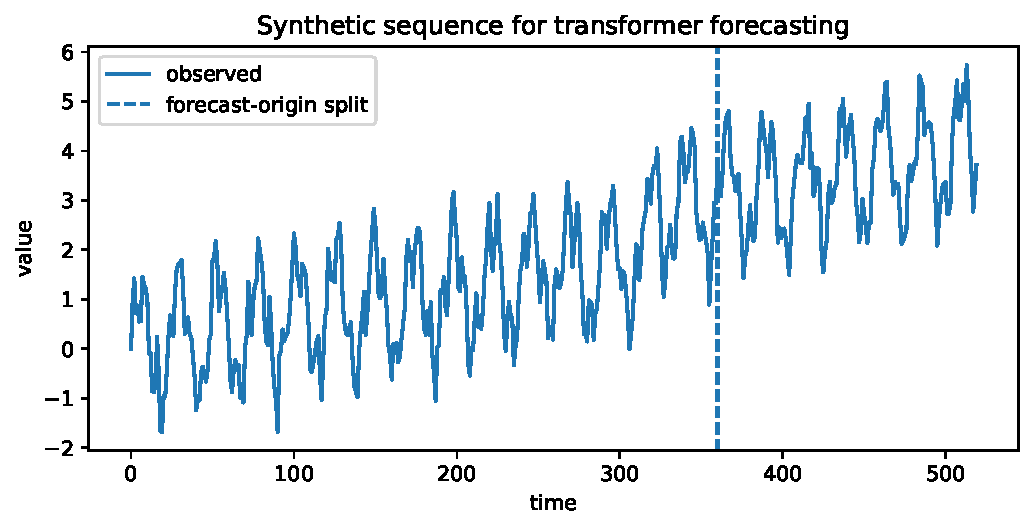
\includegraphics[keepaspectratio]{chapters/chapter-22-attention-transformers-time-series_files/figure-pdf/ch22-windowed-transformer-data-output-1.pdf}}

}

\caption{Synthetic sequence for transformer forecasting.}

\end{figure}%

\begin{verbatim}
Training windows: (325, 36)
Test windows: (154, 36)
\end{verbatim}

\protect\phantomsection\label{ch22-small-transformer-model}
\begin{Shaded}
\begin{Highlighting}[]
\ImportTok{import}\NormalTok{ torch}
\ImportTok{import}\NormalTok{ torch.nn }\ImportTok{as}\NormalTok{ nn}
\ImportTok{from}\NormalTok{ torch.utils.data }\ImportTok{import}\NormalTok{ DataLoader, TensorDataset}

\NormalTok{torch.set\_num\_threads(}\DecValTok{1}\NormalTok{)}
\NormalTok{torch.manual\_seed(}\DecValTok{222}\NormalTok{)}

\KeywordTok{def}\NormalTok{ make\_loader(X, Y, batch\_size}\OperatorTok{=}\DecValTok{32}\NormalTok{, shuffle}\OperatorTok{=}\VariableTok{False}\NormalTok{):}
\NormalTok{    X\_tensor }\OperatorTok{=}\NormalTok{ torch.tensor(X, dtype}\OperatorTok{=}\NormalTok{torch.float32).unsqueeze(}\OperatorTok{{-}}\DecValTok{1}\NormalTok{)}
\NormalTok{    Y\_tensor }\OperatorTok{=}\NormalTok{ torch.tensor(Y, dtype}\OperatorTok{=}\NormalTok{torch.float32)}
    \ControlFlowTok{return}\NormalTok{ DataLoader(TensorDataset(X\_tensor, Y\_tensor), batch\_size}\OperatorTok{=}\NormalTok{batch\_size, shuffle}\OperatorTok{=}\NormalTok{shuffle)}

\NormalTok{train\_loader }\OperatorTok{=}\NormalTok{ make\_loader(X\_train, Y\_train, shuffle}\OperatorTok{=}\VariableTok{True}\NormalTok{)}
\NormalTok{test\_loader }\OperatorTok{=}\NormalTok{ make\_loader(X\_test, Y\_test, shuffle}\OperatorTok{=}\VariableTok{False}\NormalTok{)}

\KeywordTok{class}\NormalTok{ SmallTransformerForecaster(nn.Module):}
    \KeywordTok{def} \FunctionTok{\_\_init\_\_}\NormalTok{(}\VariableTok{self}\NormalTok{, input\_dim}\OperatorTok{=}\DecValTok{1}\NormalTok{, d\_model}\OperatorTok{=}\DecValTok{24}\NormalTok{, nhead}\OperatorTok{=}\DecValTok{4}\NormalTok{, num\_layers}\OperatorTok{=}\DecValTok{1}\NormalTok{, horizon}\OperatorTok{=}\DecValTok{6}\NormalTok{, max\_len}\OperatorTok{=}\DecValTok{128}\NormalTok{):}
        \BuiltInTok{super}\NormalTok{().}\FunctionTok{\_\_init\_\_}\NormalTok{()}
        \VariableTok{self}\NormalTok{.input\_proj }\OperatorTok{=}\NormalTok{ nn.Linear(input\_dim, d\_model)}
\NormalTok{        pe }\OperatorTok{=}\NormalTok{ sinusoidal\_positional\_encoding(max\_len, d\_model)}
        \VariableTok{self}\NormalTok{.register\_buffer(}\StringTok{"pe"}\NormalTok{, torch.tensor(pe, dtype}\OperatorTok{=}\NormalTok{torch.float32).unsqueeze(}\DecValTok{0}\NormalTok{))}
\NormalTok{        layer }\OperatorTok{=}\NormalTok{ nn.TransformerEncoderLayer(}
\NormalTok{            d\_model}\OperatorTok{=}\NormalTok{d\_model,}
\NormalTok{            nhead}\OperatorTok{=}\NormalTok{nhead,}
\NormalTok{            dim\_feedforward}\OperatorTok{=}\DecValTok{48}\NormalTok{,}
\NormalTok{            dropout}\OperatorTok{=}\FloatTok{0.0}\NormalTok{,}
\NormalTok{            batch\_first}\OperatorTok{=}\VariableTok{True}\NormalTok{,}
\NormalTok{        )}
        \VariableTok{self}\NormalTok{.encoder }\OperatorTok{=}\NormalTok{ nn.TransformerEncoder(layer, num\_layers}\OperatorTok{=}\NormalTok{num\_layers)}
        \VariableTok{self}\NormalTok{.head }\OperatorTok{=}\NormalTok{ nn.Sequential(}
\NormalTok{            nn.Linear(d\_model, }\DecValTok{32}\NormalTok{),}
\NormalTok{            nn.ReLU(),}
\NormalTok{            nn.Linear(}\DecValTok{32}\NormalTok{, horizon),}
\NormalTok{        )}

    \KeywordTok{def}\NormalTok{ forward(}\VariableTok{self}\NormalTok{, x):}
        \CommentTok{\# x: batch x length x input\_dim}
\NormalTok{        z }\OperatorTok{=} \VariableTok{self}\NormalTok{.input\_proj(x)}
\NormalTok{        z }\OperatorTok{=}\NormalTok{ z }\OperatorTok{+} \VariableTok{self}\NormalTok{.pe[:, :z.shape[}\DecValTok{1}\NormalTok{], :]}
\NormalTok{        z }\OperatorTok{=} \VariableTok{self}\NormalTok{.encoder(z)}
\NormalTok{        last\_state }\OperatorTok{=}\NormalTok{ z[:, }\OperatorTok{{-}}\DecValTok{1}\NormalTok{, :]}
        \ControlFlowTok{return} \VariableTok{self}\NormalTok{.head(last\_state)}

\NormalTok{model }\OperatorTok{=}\NormalTok{ SmallTransformerForecaster(horizon}\OperatorTok{=}\NormalTok{H)}
\NormalTok{optimizer }\OperatorTok{=}\NormalTok{ torch.optim.Adam(model.parameters(), lr}\OperatorTok{=}\FloatTok{0.01}\NormalTok{)}
\NormalTok{loss\_fn }\OperatorTok{=}\NormalTok{ nn.MSELoss()}

\KeywordTok{def}\NormalTok{ evaluate(loader):}
\NormalTok{    model.}\BuiltInTok{eval}\NormalTok{()}
\NormalTok{    total, n }\OperatorTok{=} \FloatTok{0.0}\NormalTok{, }\DecValTok{0}
    \ControlFlowTok{with}\NormalTok{ torch.no\_grad():}
        \ControlFlowTok{for}\NormalTok{ xb, yb }\KeywordTok{in}\NormalTok{ loader:}
\NormalTok{            pred }\OperatorTok{=}\NormalTok{ model(xb)}
\NormalTok{            loss }\OperatorTok{=}\NormalTok{ loss\_fn(pred, yb)}
\NormalTok{            total }\OperatorTok{+=}\NormalTok{ loss.item() }\OperatorTok{*} \BuiltInTok{len}\NormalTok{(xb)}
\NormalTok{            n }\OperatorTok{+=} \BuiltInTok{len}\NormalTok{(xb)}
    \ControlFlowTok{return}\NormalTok{ total }\OperatorTok{/}\NormalTok{ n}

\ControlFlowTok{for}\NormalTok{ epoch }\KeywordTok{in} \BuiltInTok{range}\NormalTok{(}\DecValTok{8}\NormalTok{):}
\NormalTok{    model.train()}
    \ControlFlowTok{for}\NormalTok{ xb, yb }\KeywordTok{in}\NormalTok{ train\_loader:}
\NormalTok{        optimizer.zero\_grad()}
\NormalTok{        pred }\OperatorTok{=}\NormalTok{ model(xb)}
\NormalTok{        loss }\OperatorTok{=}\NormalTok{ loss\_fn(pred, yb)}
\NormalTok{        loss.backward()}
\NormalTok{        torch.nn.utils.clip\_grad\_norm\_(model.parameters(), max\_norm}\OperatorTok{=}\FloatTok{1.0}\NormalTok{)}
\NormalTok{        optimizer.step()}

    \ControlFlowTok{if}\NormalTok{ epoch }\KeywordTok{in}\NormalTok{ \{}\DecValTok{0}\NormalTok{, }\DecValTok{3}\NormalTok{, }\DecValTok{7}\NormalTok{\}:}
        \BuiltInTok{print}\NormalTok{(}\SpecialStringTok{f"epoch }\SpecialCharTok{\{}\NormalTok{epoch}\OperatorTok{+}\DecValTok{1}\SpecialCharTok{:02d\}}\SpecialStringTok{ | train MSE=}\SpecialCharTok{\{}\NormalTok{evaluate(train\_loader)}\SpecialCharTok{:.4f\}}\SpecialStringTok{ | test MSE=}\SpecialCharTok{\{}\NormalTok{evaluate(test\_loader)}\SpecialCharTok{:.4f\}}\SpecialStringTok{"}\NormalTok{)}
\end{Highlighting}
\end{Shaded}

\begin{verbatim}
epoch 01 | train MSE=0.6975 | test MSE=0.9035
epoch 04 | train MSE=0.2124 | test MSE=0.4889
epoch 08 | train MSE=0.1196 | test MSE=0.1537
\end{verbatim}

\begin{Shaded}
\begin{Highlighting}[]
\NormalTok{model.}\BuiltInTok{eval}\NormalTok{()}
\ControlFlowTok{with}\NormalTok{ torch.no\_grad():}
\NormalTok{    x\_last }\OperatorTok{=}\NormalTok{ torch.tensor(X\_test[}\OperatorTok{{-}}\DecValTok{1}\NormalTok{:], dtype}\OperatorTok{=}\NormalTok{torch.float32).unsqueeze(}\OperatorTok{{-}}\DecValTok{1}\NormalTok{)}
\NormalTok{    pred\_scaled }\OperatorTok{=}\NormalTok{ model(x\_last).numpy()}

\NormalTok{pred }\OperatorTok{=}\NormalTok{ y\_scaler.inverse\_transform(pred\_scaled)[}\DecValTok{0}\NormalTok{]}
\NormalTok{true }\OperatorTok{=}\NormalTok{ y\_scaler.inverse\_transform(Y\_test[}\OperatorTok{{-}}\DecValTok{1}\NormalTok{:])[}\DecValTok{0}\NormalTok{]}
\NormalTok{input\_original }\OperatorTok{=}\NormalTok{ x\_scaler.inverse\_transform(X\_test[}\OperatorTok{{-}}\DecValTok{1}\NormalTok{:])[}\DecValTok{0}\NormalTok{]}

\CommentTok{\# Seasonal naive baseline using lag 24 when available.}
\NormalTok{seasonal\_naive }\OperatorTok{=}\NormalTok{ input\_original[}\OperatorTok{{-}}\DecValTok{24}\NormalTok{:}\OperatorTok{{-}}\DecValTok{24} \OperatorTok{+}\NormalTok{ H]}
\ControlFlowTok{if} \BuiltInTok{len}\NormalTok{(seasonal\_naive) }\OperatorTok{\textless{}}\NormalTok{ H:}
\NormalTok{    seasonal\_naive }\OperatorTok{=}\NormalTok{ np.repeat(input\_original[}\OperatorTok{{-}}\DecValTok{1}\NormalTok{], H)}

\NormalTok{rmse\_transformer }\OperatorTok{=}\NormalTok{ np.sqrt(np.mean((pred }\OperatorTok{{-}}\NormalTok{ true) }\OperatorTok{**} \DecValTok{2}\NormalTok{))}
\NormalTok{rmse\_naive }\OperatorTok{=}\NormalTok{ np.sqrt(np.mean((seasonal\_naive }\OperatorTok{{-}}\NormalTok{ true) }\OperatorTok{**} \DecValTok{2}\NormalTok{))}
\BuiltInTok{print}\NormalTok{(}\StringTok{"Transformer RMSE on displayed window:"}\NormalTok{, }\BuiltInTok{round}\NormalTok{(}\BuiltInTok{float}\NormalTok{(rmse\_transformer), }\DecValTok{3}\NormalTok{))}
\BuiltInTok{print}\NormalTok{(}\StringTok{"Seasonal naive RMSE on displayed window:"}\NormalTok{, }\BuiltInTok{round}\NormalTok{(}\BuiltInTok{float}\NormalTok{(rmse\_naive), }\DecValTok{3}\NormalTok{))}

\NormalTok{history\_x }\OperatorTok{=}\NormalTok{ np.arange(L)}
\NormalTok{future\_x }\OperatorTok{=}\NormalTok{ np.arange(L, L }\OperatorTok{+}\NormalTok{ H)}

\NormalTok{plt.figure(figsize}\OperatorTok{=}\NormalTok{(}\DecValTok{8}\NormalTok{, }\FloatTok{3.5}\NormalTok{))}
\NormalTok{plt.plot(history\_x, input\_original, label}\OperatorTok{=}\StringTok{"input window"}\NormalTok{)}
\NormalTok{plt.plot(future\_x, true, marker}\OperatorTok{=}\StringTok{"o"}\NormalTok{, label}\OperatorTok{=}\StringTok{"true future"}\NormalTok{)}
\NormalTok{plt.plot(future\_x, pred, marker}\OperatorTok{=}\StringTok{"o"}\NormalTok{, label}\OperatorTok{=}\StringTok{"transformer forecast"}\NormalTok{)}
\NormalTok{plt.plot(future\_x, seasonal\_naive, marker}\OperatorTok{=}\StringTok{"o"}\NormalTok{, label}\OperatorTok{=}\StringTok{"seasonal naive"}\NormalTok{)}
\NormalTok{plt.axvline(L }\OperatorTok{{-}} \DecValTok{1}\NormalTok{, linestyle}\OperatorTok{=}\StringTok{"{-}{-}"}\NormalTok{)}
\NormalTok{plt.xlabel(}\StringTok{"relative time"}\NormalTok{)}
\NormalTok{plt.ylabel(}\StringTok{"value"}\NormalTok{)}
\NormalTok{plt.title(}\StringTok{"Held{-}out multi{-}step forecast"}\NormalTok{)}
\NormalTok{plt.legend()}
\NormalTok{plt.show()}
\end{Highlighting}
\end{Shaded}

\begin{verbatim}
Transformer RMSE on displayed window: 0.477
Seasonal naive RMSE on displayed window: 0.864
\end{verbatim}

\begin{figure}[H]

{\centering \pandocbounded{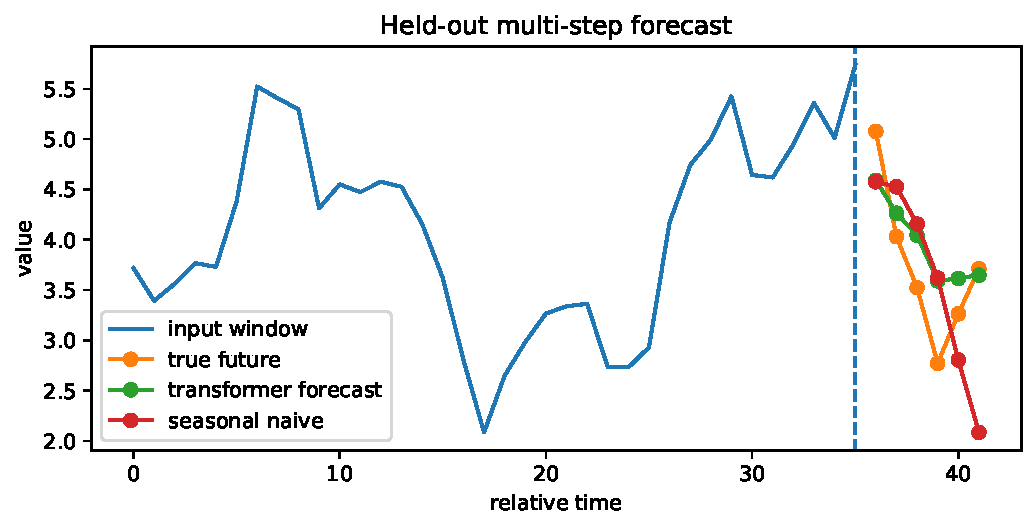
\includegraphics[keepaspectratio]{chapters/chapter-22-attention-transformers-time-series_files/figure-pdf/ch22-transformer-vs-baseline-output-2.pdf}}

}

\caption{One held-out transformer forecast compared with a seasonal
naive baseline.}

\end{figure}%

\section{22.16 Diagnostics and
interpretation}\label{diagnostics-and-interpretation}

A transformer forecast should be judged as part of a forecasting
workflow, not as an isolated deep-learning demonstration.

Key diagnostics include:

\begin{itemize}
\tightlist
\item
  comparison against naive, seasonal naive, ARIMA/SARIMA, and
  feature-based ML baselines;
\item
  horizon-wise error curves;
\item
  residual plots over time;
\item
  error stratified by regime, season, or magnitude;
\item
  stability over rolling-origin backtests;
\item
  sensitivity to input length \(L\) and horizon \(H\);
\item
  evidence that masking and chronological splits prevent leakage.
\end{itemize}

Attention heatmaps can be useful for debugging. For example, if a model
always attends only to the most recent value, a simpler autoregressive
or convolutional model may suffice. If it attends to future positions in
a forecasting task, the model is leaking.

\section{22.17 AI-assisted model
critique}\label{ai-assisted-model-critique-1}

\section{AI-assisted study box}\label{ai-assisted-study-box-1}

Give an AI assistant a transformer forecasting script and ask it to
check the following. Then verify every answer yourself.

\begin{enumerate}
\def\labelenumi{\arabic{enumi}.}
\tightlist
\item
  Which tensors represent known inputs and which tensors represent
  labels?
\item
  Is the train/test split chronological?
\item
  Is the scaler fit only on training data?
\item
  Does the attention mask forbid future information when needed?
\item
  What baseline should be used before claiming improvement?
\item
  What is the forecast horizon, and how is horizon-wise error computed?
\item
  Is the model size appropriate for the number of training windows?
\item
  What failure mode is most likely for this data set?
\end{enumerate}

A useful prompt is:

\begin{quote}
I am training a transformer for time-series forecasting. Please inspect
the code for data leakage, incorrect tensor shapes, missing causal
masks, and inappropriate validation. For each issue, quote the line or
operation that causes the problem and propose a corrected version. Do
not judge the model only by training loss.
\end{quote}

\section{22.18 Common mistakes}\label{common-mistakes-21}

\begin{enumerate}
\def\labelenumi{\arabic{enumi}.}
\tightlist
\item
  \textbf{Forgetting position information.} Self-attention needs a way
  to know order.
\item
  \textbf{Using future values by accident.} Incorrect masks or window
  construction can leak labels.
\item
  \textbf{Random train-test splits.} Random splits destroy the
  forecasting interpretation.
\item
  \textbf{Comparing only with weak baselines.} A transformer should beat
  seasonal naive and strong feature-based models before it is considered
  useful.
\item
  \textbf{Using too large a model.} A transformer can overfit small
  time-series data sets quickly.
\item
  \textbf{Treating attention as proof of causality.} Attention weights
  show model-internal weighting, not causal explanation.
\item
  \textbf{Ignoring horizon-wise performance.} A model may do well at
  \(h=1\) and poorly at \(h=H\).
\item
  \textbf{Confusing encoder and decoder masks.} Encoder-style window
  forecasting may not need an internal causal mask if the input window
  contains only known history. Autoregressive decoding does need causal
  masking.
\end{enumerate}

\section{22.19 Exercises}\label{exercises-21}

\begin{enumerate}
\def\labelenumi{\arabic{enumi}.}
\tightlist
\item
  Compute the scaled dot-product attention matrix for a sequence of
  length \(T=4\) with \(d_k=2\) using given query and key matrices. Then
  apply a causal mask.
\item
  Prove that adding the same constant to every score in one row of the
  attention matrix does not change the softmax weights.
\item
  Explain why self-attention without positional encoding is
  permutation-equivariant.
\item
  Implement sinusoidal positional encoding for \(d_{\text{model}}=8\)
  and plot all components for \(T=100\).
\item
  Modify the NumPy attention example so that each query attends only to
  the previous \(w\) time steps. Compare this local attention mask with
  the full causal mask.
\item
  Train the small transformer forecaster with \(L=24,36,72\). Compare
  horizon-wise RMSE.
\item
  Replace the transformer with an MLP, CNN, or LSTM using the same
  windows and split. Which model wins?
\item
  For a data set with strong weekly seasonality, design input features
  that make the transformer aware of the day of week.
\item
  Construct an example where a transformer overfits the training data
  but fails on a rolling-origin test.
\item
  Write an AI-assisted critique report that identifies at least three
  possible leakage points in a transformer forecasting pipeline.
\end{enumerate}

\section{22.20 Mini project}\label{mini-project-5}

Choose a univariate or multivariate time series with at least one
seasonal or regime-like structure. Build a transformer-based forecasting
workflow.

Your report should include:

\begin{enumerate}
\def\labelenumi{\arabic{enumi}.}
\tightlist
\item
  a description of the data and forecasting target;
\item
  a chronological train/validation/test design;
\item
  at least three baselines, including naive or seasonal naive;
\item
  a transformer model with clear input length \(L\), horizon \(H\),
  model dimension, number of heads, and number of layers;
\item
  horizon-wise error metrics;
\item
  one attention or representation diagnostic;
\item
  a discussion of whether the transformer is justified compared with
  simpler models;
\item
  an AI-assisted critique section where you state what an AI tool
  suggested and how you verified or corrected it.
\end{enumerate}

\section{22.21 Checklist}\label{checklist-6}

Before moving on, make sure you can answer the following questions.

\begin{itemize}
\tightlist
\item
  What are \(Q\), \(K\), and \(V\)?
\item
  Why do we divide \(QK^T\) by \(\sqrt{d_k}\)?
\item
  What does a causal mask do mathematically?
\item
  Why does a transformer need position information?
\item
  How does multi-head attention differ from single-head attention?
\item
  What are the main components of a transformer block?
\item
  When does an encoder-style forecast model need a causal mask?
\item
  How should a transformer forecast be validated?
\item
  What baselines should be used before claiming improvement?
\item
  What can and cannot be concluded from attention weights?
\end{itemize}

\chapter{Representation Learning for Time
Series}\label{representation-learning-for-time-series}

\textbf{Part VI. Deep Learning for Time Series and Sequence Data}\\
\textbf{Chapter goal:} understand how modern models learn useful
representations of time series. We study window embeddings,
autoencoders, masked reconstruction, contrastive learning, anomaly
detection, clustering, retrieval, validation, and AI-assisted
representation diagnosis.

\section{Learning objectives}\label{learning-objectives-22}

After studying this chapter, you should be able to:

\begin{enumerate}
\def\labelenumi{\arabic{enumi}.}
\tightlist
\item
  explain what a learned representation is and why it is useful for
  forecasting, classification, clustering, retrieval, and anomaly
  detection;
\item
  formulate a time-series encoder as a map from an observed window to a
  latent vector;
\item
  distinguish handcrafted features, linear embeddings, autoencoder
  embeddings, and self-supervised embeddings;
\item
  derive the reconstruction objective for an autoencoder and relate a
  linear autoencoder to PCA;
\item
  use latent embeddings for clustering, nearest-neighbor search, and
  anomaly detection;
\item
  describe masked reconstruction and contrastive learning as pretext
  tasks for unlabeled sequence data;
\item
  identify validation leakage in representation-learning pipelines;
\item
  implement simple representation-learning workflows in Python;
\item
  use AI tools to critique representation quality while verifying the
  assumptions mathematically and computationally.
\end{enumerate}

\section{23.1 Motivation: from prediction to
representation}\label{motivation-from-prediction-to-representation}

In earlier chapters, we built models that map a past window directly to
a forecast. For example, a supervised forecaster may use

\[
(y_{t-L+1},\ldots,y_t) \mapsto \widehat y_{t+h}.
\]

Representation learning introduces an intermediate object. Instead of
mapping the observed window directly to an output, we first encode the
window into a lower-dimensional vector:

\[
\mathbf z_t = f_\theta(\mathbf x_t),
\]

where

\[
\mathbf x_t = (y_{t-L+1},\ldots,y_t)^T \in \mathbb R^L,
\qquad
\mathbf z_t \in \mathbb R^d,
\qquad d \ll L.
\]

The vector \(\mathbf z_t\) is called a \textbf{representation},
\textbf{embedding}, or \textbf{latent feature vector}. The
representation can then be used for many tasks:

\[
\text{forecasting: } \widehat y_{t+h}=g_\phi(\mathbf z_t),
\]

\[
\text{classification: } \widehat c_t = h_\psi(\mathbf z_t),
\]

\[
\text{anomaly detection: } a_t = A(\mathbf z_t),
\]

\[
\text{retrieval: } \operatorname{similarity}(\mathbf x_i,\mathbf x_j)
= \operatorname{similarity}(\mathbf z_i,\mathbf z_j).
\]

The key idea is that a good representation should keep information that
matters for the task and discard nuisance variation such as irrelevant
noise, arbitrary phase shifts, or small measurement errors.

\begin{tcolorbox}[enhanced jigsaw, arc=.35mm, bottomrule=.15mm, bottomtitle=1mm, breakable, colback=white, colbacktitle=quarto-callout-note-color!10!white, colframe=quarto-callout-note-color-frame, coltitle=black, left=2mm, leftrule=.75mm, opacityback=0, opacitybacktitle=0.6, rightrule=.15mm, title=\textcolor{quarto-callout-note-color}{\faInfo}\hspace{0.5em}{Connection with the previous chapters}, titlerule=0mm, toprule=.15mm, toptitle=1mm]

A representation can be produced by many architectures: handcrafted
statistical features, PCA, convolutional encoders, recurrent encoders,
attention encoders, autoencoders, or self-supervised transformers. The
representation-learning viewpoint unifies classical feature engineering
and modern deep sequence learning.

\end{tcolorbox}

\section{23.2 Windows, encoders, and latent
spaces}\label{windows-encoders-and-latent-spaces}

Let \(\{y_t\}_{t=1}^T\) be a univariate time series. A standard first
step is to create overlapping windows

\[
\mathbf x_i = (y_i,y_{i+1},\ldots,y_{i+L-1})^T,
\qquad i=1,\ldots,N,
\]

where \(N=T-L+1\). For a multivariate time series
\(\mathbf y_t\in\mathbb R^p\), a window is a matrix

\[
X_i =
\begin{bmatrix}
\mathbf y_i^T\\
\mathbf y_{i+1}^T\\
\vdots\\
\mathbf y_{i+L-1}^T
\end{bmatrix}
\in \mathbb R^{L\times p}.
\]

An encoder is a function

\[
f_\theta: \mathbb R^{L\times p}\to \mathbb R^d.
\]

Examples include:

\[
f_\theta(X_i)=\text{handcrafted features},
\]

\[
f_\theta(X_i)=W\operatorname{vec}(X_i)+\mathbf b,
\]

\[
f_\theta(X_i)=\text{CNN}(X_i),
\]

\[
f_\theta(X_i)=\text{RNN}(X_i),
\]

\[
f_\theta(X_i)=\text{Transformer}(X_i).
\]

The latent space \(\mathbb R^d\) is useful only if geometric
relationships in latent space correspond to meaningful relationships
between sequences. A common hope is:

\[
\|\mathbf z_i-\mathbf z_j\| \text{ small}
\quad \Longrightarrow \quad
X_i \text{ and } X_j \text{ have similar behavior}.
\]

But this implication is not automatic. It depends on the training
objective, preprocessing, windowing scheme, and validation design.

\section{23.3 Handcrafted
representations}\label{handcrafted-representations}

Before training a neural representation model, it is useful to
understand handcrafted representations. For a window
\(\mathbf x=(x_1,\ldots,x_L)^T\), we may compute features such as

\[
\widehat \mu = \frac1L\sum_{t=1}^L x_t,
\]

\[
\widehat \sigma^2 = \frac1L\sum_{t=1}^L (x_t-\widehat\mu)^2,
\]

\[
\widehat\rho(1)=
\frac{\sum_{t=2}^L (x_t-\widehat\mu)(x_{t-1}-\widehat\mu)}
{\sum_{t=1}^L (x_t-\widehat\mu)^2},
\]

and frequency features such as

\[
A(\omega)=\left|\sum_{t=1}^L x_t e^{-2\pi i \omega t}\right|.
\]

A feature map might be

\[
\Phi(\mathbf x)=
\big(\widehat \mu,\widehat\sigma,\widehat\rho(1),A(\omega_1),A(\omega_2),\ldots\big)^T.
\]

This is a representation. It is not learned, but it already maps a raw
sequence window into a lower-dimensional vector.

\begin{tcolorbox}[enhanced jigsaw, arc=.35mm, bottomrule=.15mm, bottomtitle=1mm, breakable, colback=white, colbacktitle=quarto-callout-tip-color!10!white, colframe=quarto-callout-tip-color-frame, coltitle=black, left=2mm, leftrule=.75mm, opacityback=0, opacitybacktitle=0.6, rightrule=.15mm, title=\textcolor{quarto-callout-tip-color}{\faLightbulb}\hspace{0.5em}{Why start with handcrafted features?}, titlerule=0mm, toprule=.15mm, toptitle=1mm]

Handcrafted features are interpretable baselines. If a deep embedding
does not outperform simple features such as mean, variance,
autocorrelation, trend slope, and spectral energy, then the deep model
may not be adding value.

\end{tcolorbox}

\section{23.4 Linear representations and
PCA}\label{linear-representations-and-pca}

Suppose we form a matrix of centered windows

\[
X=
\begin{bmatrix}
\mathbf x_1^T\\
\mathbf x_2^T\\
\vdots\\
\mathbf x_N^T
\end{bmatrix}
\in\mathbb R^{N\times L}.
\]

Principal component analysis finds orthonormal directions
\(\mathbf v_1,\ldots,\mathbf v_d\) that maximize projected variance. The
representation of window \(\mathbf x_i\) is

\[
\mathbf z_i=
\begin{bmatrix}
\mathbf v_1^T\mathbf x_i\\
\vdots\\
\mathbf v_d^T\mathbf x_i
\end{bmatrix}.
\]

Equivalently, if \(V_d=[\mathbf v_1,\ldots,\mathbf v_d]\), then

\[
\mathbf z_i = V_d^T\mathbf x_i,
\qquad
\widehat{\mathbf x}_i = V_d\mathbf z_i.
\]

The reconstruction error is

\[
\|\mathbf x_i-\widehat{\mathbf x}_i\|_2^2.
\]

PCA is a representation-learning method with a closed-form solution. It
is linear, unsupervised, and useful as a baseline for autoencoders.

\section{23.5 Autoencoders}\label{autoencoders}

An autoencoder learns an encoder and a decoder:

\[
\mathbf z_i=f_\theta(\mathbf x_i),
\qquad
\widehat{\mathbf x}_i=g_\phi(\mathbf z_i).
\]

The training objective is usually reconstruction loss:

\[
\min_{\theta,\phi}\frac1N\sum_{i=1}^N
\|\mathbf x_i-g_\phi(f_\theta(\mathbf x_i))\|_2^2.
\]

If \(d<L\), then the model is forced to compress the window through a
bottleneck. A good bottleneck may retain trend, oscillation, local
shape, volatility, and regime information while discarding small noise.

For a neural autoencoder, the encoder may be an MLP, CNN, RNN, or
transformer:

\[
f_\theta(\mathbf x)=F_K\circ F_{K-1}\circ\cdots\circ F_1(\mathbf x).
\]

The decoder maps the latent vector back to the window space. For
sequence data, the decoder may produce an entire reconstructed sequence.

\begin{tcolorbox}[enhanced jigsaw, arc=.35mm, bottomrule=.15mm, bottomtitle=1mm, breakable, colback=white, colbacktitle=quarto-callout-warning-color!10!white, colframe=quarto-callout-warning-color-frame, coltitle=black, left=2mm, leftrule=.75mm, opacityback=0, opacitybacktitle=0.6, rightrule=.15mm, title=\textcolor{quarto-callout-warning-color}{\faExclamationTriangle}\hspace{0.5em}{Reconstruction is not the same as usefulness}, titlerule=0mm, toprule=.15mm, toptitle=1mm]

A representation with low reconstruction error is not necessarily good
for forecasting or classification. It may waste latent capacity
reconstructing irrelevant noise. Always evaluate the representation on
the downstream task or on a carefully chosen proxy task.

\end{tcolorbox}

\section{23.6 Interactive module: embedding
explorer}\label{interactive-module-embedding-explorer}

This module creates synthetic windows from several time-series families.
It maps each window to a two-dimensional feature embedding. The purpose
is to show that even simple features can separate different temporal
behaviors.

Interactive Module: Time-Series Embedding Explorer

Change the window length and noise level. Click points in the embedding
to inspect the corresponding time-series window.

Window length L:
\protect\phantomsection\label{ch23_embed_length_value}{80}

Noise level: \protect\phantomsection\label{ch23_embed_noise_value}{0.35}

Random seed: \protect\phantomsection\label{ch23_embed_seed_value}{7}

\protect\phantomsection\label{ch23_embedding_plot}

\protect\phantomsection\label{ch23_selected_window_plot}

The interactive embedding is deliberately simple. A deep encoder tries
to learn a better map \(f_\theta\) automatically, but the same question
remains: does the geometry of the embedding reflect meaningful
time-series structure?

\section{23.7 Interactive module: bottlenecks and
reconstruction}\label{interactive-module-bottlenecks-and-reconstruction}

This module uses a Fourier bottleneck as an interpretable analogue of a
linear autoencoder. Keeping only a few smooth components reconstructs
the large-scale pattern but misses spikes and high-frequency details.
This illustrates why reconstruction error can be useful for anomaly
detection.

Interactive Module: Bottleneck Reconstruction and Anomaly Score

Increase the latent dimension to make the reconstruction more flexible.
Increase the anomaly size to see how residual error changes.

Latent dimension k:
\protect\phantomsection\label{ch23_bottleneck_k_value}{5}

Anomaly size:
\protect\phantomsection\label{ch23_bottleneck_anomaly_value}{2.50}

Noise level:
\protect\phantomsection\label{ch23_bottleneck_noise_value}{0.20}

\protect\phantomsection\label{ch23_bottleneck_reconstruction_plot}

\protect\phantomsection\label{ch23_bottleneck_error_plot}

\section{23.8 Self-supervised learning for time
series}\label{self-supervised-learning-for-time-series}

A major reason representation learning is important is that labeled
sequence data are often expensive, while unlabeled sequence data are
abundant. Self-supervised learning creates artificial training tasks
from the data itself.

\subsection{Masked reconstruction}\label{masked-reconstruction}

Given a window \(\mathbf x_i\), choose a mask
\(M_i\subset\{1,\ldots,L\}\). The model receives a corrupted version
\(\widetilde{\mathbf x}_i\) and must reconstruct the hidden entries:

\[
\min_{\theta}\sum_i \sum_{t\in M_i}
\left(x_{i,t}-\widehat x_{i,t}\right)^2.
\]

This teaches the encoder to use surrounding context. For time series,
masks may hide isolated points, contiguous blocks, channels, or future
values.

\subsection{Forecasting as a pretext
task}\label{forecasting-as-a-pretext-task}

A representation may also be trained by predicting the near future:

\[
\mathbf z_t=f_\theta(y_{t-L+1:t}),
\qquad
\widehat y_{t+1:t+H}=g_\phi(\mathbf z_t),
\]

with loss

\[
\min_{\theta,\phi}\sum_t
\left\|y_{t+1:t+H}-g_\phi(f_\theta(y_{t-L+1:t}))\right\|_2^2.
\]

After training, the encoder \(f_\theta\) can be reused for clustering,
anomaly detection, or classification.

\subsection{Contrastive learning}\label{contrastive-learning}

Contrastive learning constructs pairs. A positive pair should have
similar embeddings; a negative pair should have different embeddings.
For example, \(\mathbf x_i\) and an augmented version \(a(\mathbf x_i)\)
form a positive pair. Other windows form negative pairs.

A common contrastive objective is the InfoNCE loss:

\[
\mathcal L_i
= -\log
\frac{\exp(\operatorname{sim}(\mathbf z_i,\mathbf z_i^+)/\tau)}
{\exp(\operatorname{sim}(\mathbf z_i,\mathbf z_i^+)/\tau)+
\sum_{j\in\mathcal N_i}\exp(\operatorname{sim}(\mathbf z_i,\mathbf z_j^-)/\tau)}.
\]

Here \(\tau>0\) is a temperature parameter and \(\operatorname{sim}\) is
often cosine similarity:

\[
\operatorname{sim}(\mathbf a,\mathbf b)=
\frac{\mathbf a^T\mathbf b}{\|\mathbf a\|_2\|\mathbf b\|_2}.
\]

The choice of augmentation is crucial. Reasonable time-series
augmentations may include small jitter, scaling, time masking,
crop-and-resize, or frequency perturbation. But augmentations must
preserve the label-relevant structure.

\begin{tcolorbox}[enhanced jigsaw, arc=.35mm, bottomrule=.15mm, bottomtitle=1mm, breakable, colback=white, colbacktitle=quarto-callout-warning-color!10!white, colframe=quarto-callout-warning-color-frame, coltitle=black, left=2mm, leftrule=.75mm, opacityback=0, opacitybacktitle=0.6, rightrule=.15mm, title=\textcolor{quarto-callout-warning-color}{\faExclamationTriangle}\hspace{0.5em}{Augmentation can change the meaning}, titlerule=0mm, toprule=.15mm, toptitle=1mm]

For ECG data, small timing changes may preserve the medical label, but
aggressive time warping may destroy clinically important intervals. For
finance, shuffling destroys temporal dependence. For forecasting, using
future values inside an augmentation can leak information.

\end{tcolorbox}

\section{23.9 Anomaly detection with
representations}\label{anomaly-detection-with-representations}

Representation learning is often used for anomaly detection. A common
autoencoder score is reconstruction error:

\[
a_i=\|\mathbf x_i-\widehat{\mathbf x}_i\|_2^2.
\]

If the model is trained mostly on normal behavior, anomalous windows may
have larger error because they do not lie near the learned normal
manifold.

Another approach is latent-distance scoring. Let
\(\widehat{\boldsymbol\mu}\) and \(\widehat\Sigma\) be the empirical
mean and covariance of normal latent vectors. Then a Mahalanobis score
is

\[
a_i=(\mathbf z_i-\widehat{\boldsymbol\mu})^T
\widehat\Sigma^{-1}
(\mathbf z_i-\widehat{\boldsymbol\mu}).
\]

Large values indicate that the latent vector is far from the normal
latent distribution.

For sequence anomalies, the score should often be attached to a time
interval rather than a single time point. If a window score \(a_i\)
corresponds to window \(i:i+L-1\), then one can aggregate scores over
windows covering time \(t\):

\[
A_t=\frac{1}{|\mathcal W_t|}\sum_{i\in\mathcal W_t}a_i,
\]

where \(\mathcal W_t\) is the set of windows containing time \(t\).

\section{23.10 Representation quality: what should be
checked?}\label{representation-quality-what-should-be-checked}

A representation should be evaluated in relation to a task. Useful
checks include:

\begin{enumerate}
\def\labelenumi{\arabic{enumi}.}
\tightlist
\item
  \textbf{Baseline comparison.} Does the learned representation
  outperform simple features or PCA?
\item
  \textbf{Temporal validation.} Were all transformations fitted only on
  training data?
\item
  \textbf{Neighborhood quality.} Do nearest neighbors in latent space
  look similar in the original time domain?
\item
  \textbf{Downstream usefulness.} Does the representation improve
  forecasting, classification, retrieval, or anomaly detection?
\item
  \textbf{Stability.} Does the embedding change dramatically with random
  seed or small perturbations?
\item
  \textbf{Interpretability.} Can latent dimensions be related to trend,
  periodicity, volatility, or regime?
\item
  \textbf{Leakage audit.} Did any representation step use future values,
  test labels, global scaling, or windows crossing the train-test
  boundary?
\end{enumerate}

\begin{tcolorbox}[enhanced jigsaw, arc=.35mm, bottomrule=.15mm, bottomtitle=1mm, breakable, colback=white, colbacktitle=quarto-callout-important-color!10!white, colframe=quarto-callout-important-color-frame, coltitle=black, left=2mm, leftrule=.75mm, opacityback=0, opacitybacktitle=0.6, rightrule=.15mm, title=\textcolor{quarto-callout-important-color}{\faExclamation}\hspace{0.5em}{Leakage in representation learning}, titlerule=0mm, toprule=.15mm, toptitle=1mm]

Representation learning is especially vulnerable to leakage. Scaling,
PCA, autoencoder training, contrastive pair construction, and imputation
must be fitted using training data only when evaluating predictive
performance.

\end{tcolorbox}

\section{23.11 Python example: handcrafted features and PCA
embeddings}\label{python-example-handcrafted-features-and-pca-embeddings}

The following example creates synthetic windows from four families and
embeds them using simple features followed by PCA.

\begin{Shaded}
\begin{Highlighting}[]
\ImportTok{import}\NormalTok{ numpy }\ImportTok{as}\NormalTok{ np}
\ImportTok{import}\NormalTok{ matplotlib.pyplot }\ImportTok{as}\NormalTok{ plt}
\ImportTok{from}\NormalTok{ sklearn.decomposition }\ImportTok{import}\NormalTok{ PCA}
\ImportTok{from}\NormalTok{ sklearn.preprocessing }\ImportTok{import}\NormalTok{ StandardScaler}

\NormalTok{rng }\OperatorTok{=}\NormalTok{ np.random.default\_rng(}\DecValTok{7}\NormalTok{)}
\NormalTok{L }\OperatorTok{=} \DecValTok{80}
\NormalTok{n\_per\_class }\OperatorTok{=} \DecValTok{70}

\KeywordTok{def}\NormalTok{ make\_window(kind, L}\OperatorTok{=}\DecValTok{80}\NormalTok{, rng}\OperatorTok{=}\VariableTok{None}\NormalTok{, noise}\OperatorTok{=}\FloatTok{0.30}\NormalTok{):}
    \ControlFlowTok{if}\NormalTok{ rng }\KeywordTok{is} \VariableTok{None}\NormalTok{:}
\NormalTok{        rng }\OperatorTok{=}\NormalTok{ np.random.default\_rng()}
\NormalTok{    t }\OperatorTok{=}\NormalTok{ np.arange(L)}
\NormalTok{    phase }\OperatorTok{=}\NormalTok{ rng.uniform(}\DecValTok{0}\NormalTok{, }\DecValTok{2}\OperatorTok{*}\NormalTok{np.pi)}

    \ControlFlowTok{if}\NormalTok{ kind }\OperatorTok{==} \StringTok{"low\_frequency"}\NormalTok{:}
\NormalTok{        x }\OperatorTok{=}\NormalTok{ np.sin(}\DecValTok{2}\OperatorTok{*}\NormalTok{np.pi}\OperatorTok{*}\NormalTok{t}\OperatorTok{/}\DecValTok{40} \OperatorTok{+}\NormalTok{ phase)}
    \ControlFlowTok{elif}\NormalTok{ kind }\OperatorTok{==} \StringTok{"high\_frequency"}\NormalTok{:}
\NormalTok{        x }\OperatorTok{=}\NormalTok{ np.sin(}\DecValTok{2}\OperatorTok{*}\NormalTok{np.pi}\OperatorTok{*}\NormalTok{t}\OperatorTok{/}\DecValTok{10} \OperatorTok{+}\NormalTok{ phase)}
    \ControlFlowTok{elif}\NormalTok{ kind }\OperatorTok{==} \StringTok{"trend"}\NormalTok{:}
\NormalTok{        slope }\OperatorTok{=}\NormalTok{ rng.uniform(}\FloatTok{0.015}\NormalTok{, }\FloatTok{0.035}\NormalTok{)}
\NormalTok{        x }\OperatorTok{=}\NormalTok{ slope}\OperatorTok{*}\NormalTok{t }\OperatorTok{+} \FloatTok{0.25}\OperatorTok{*}\NormalTok{np.sin(}\DecValTok{2}\OperatorTok{*}\NormalTok{np.pi}\OperatorTok{*}\NormalTok{t}\OperatorTok{/}\DecValTok{25} \OperatorTok{+}\NormalTok{ phase)}
    \ControlFlowTok{elif}\NormalTok{ kind }\OperatorTok{==} \StringTok{"spike"}\NormalTok{:}
\NormalTok{        x }\OperatorTok{=} \FloatTok{0.6}\OperatorTok{*}\NormalTok{np.sin(}\DecValTok{2}\OperatorTok{*}\NormalTok{np.pi}\OperatorTok{*}\NormalTok{t}\OperatorTok{/}\DecValTok{30} \OperatorTok{+}\NormalTok{ phase)}
\NormalTok{        center }\OperatorTok{=}\NormalTok{ rng.integers(L}\OperatorTok{//}\DecValTok{4}\NormalTok{, }\DecValTok{3}\OperatorTok{*}\NormalTok{L}\OperatorTok{//}\DecValTok{4}\NormalTok{)}
\NormalTok{        x[center:center}\OperatorTok{+}\DecValTok{3}\NormalTok{] }\OperatorTok{+=}\NormalTok{ rng.uniform(}\FloatTok{2.0}\NormalTok{, }\FloatTok{3.5}\NormalTok{)}
    \ControlFlowTok{else}\NormalTok{:}
        \ControlFlowTok{raise} \PreprocessorTok{ValueError}\NormalTok{(}\StringTok{"unknown kind"}\NormalTok{)}

\NormalTok{    x }\OperatorTok{=}\NormalTok{ x }\OperatorTok{+}\NormalTok{ noise}\OperatorTok{*}\NormalTok{rng.normal(size}\OperatorTok{=}\NormalTok{L)}
    \ControlFlowTok{return}\NormalTok{ (x }\OperatorTok{{-}}\NormalTok{ x.mean()) }\OperatorTok{/}\NormalTok{ (x.std() }\OperatorTok{+} \FloatTok{1e{-}12}\NormalTok{)}

\KeywordTok{def}\NormalTok{ acf1(x):}
\NormalTok{    x }\OperatorTok{=}\NormalTok{ x }\OperatorTok{{-}}\NormalTok{ x.mean()}
\NormalTok{    denom }\OperatorTok{=}\NormalTok{ np.dot(x, x)}
    \ControlFlowTok{return}\NormalTok{ np.dot(x[}\DecValTok{1}\NormalTok{:], x[:}\OperatorTok{{-}}\DecValTok{1}\NormalTok{]) }\OperatorTok{/}\NormalTok{ denom }\ControlFlowTok{if}\NormalTok{ denom }\OperatorTok{\textgreater{}} \DecValTok{0} \ControlFlowTok{else} \FloatTok{0.0}

\KeywordTok{def}\NormalTok{ spectral\_amp(x, period):}
\NormalTok{    t }\OperatorTok{=}\NormalTok{ np.arange(}\BuiltInTok{len}\NormalTok{(x))}
\NormalTok{    c }\OperatorTok{=}\NormalTok{ np.cos(}\DecValTok{2}\OperatorTok{*}\NormalTok{np.pi}\OperatorTok{*}\NormalTok{t}\OperatorTok{/}\NormalTok{period)}
\NormalTok{    s }\OperatorTok{=}\NormalTok{ np.sin(}\DecValTok{2}\OperatorTok{*}\NormalTok{np.pi}\OperatorTok{*}\NormalTok{t}\OperatorTok{/}\NormalTok{period)}
    \ControlFlowTok{return}\NormalTok{ np.sqrt(np.dot(x, c)}\OperatorTok{**}\DecValTok{2} \OperatorTok{+}\NormalTok{ np.dot(x, s)}\OperatorTok{**}\DecValTok{2}\NormalTok{) }\OperatorTok{/} \BuiltInTok{len}\NormalTok{(x)}

\KeywordTok{def}\NormalTok{ features(x):}
\NormalTok{    t }\OperatorTok{=}\NormalTok{ np.arange(}\BuiltInTok{len}\NormalTok{(x))}
\NormalTok{    slope }\OperatorTok{=}\NormalTok{ np.polyfit(t, x, }\DecValTok{1}\NormalTok{)[}\DecValTok{0}\NormalTok{]}
    \ControlFlowTok{return}\NormalTok{ np.array([}
\NormalTok{        x.mean(),}
\NormalTok{        x.std(),}
\NormalTok{        acf1(x),}
\NormalTok{        slope,}
\NormalTok{        spectral\_amp(x, }\DecValTok{40}\NormalTok{),}
\NormalTok{        spectral\_amp(x, }\DecValTok{10}\NormalTok{),}
\NormalTok{        np.}\BuiltInTok{max}\NormalTok{(np.}\BuiltInTok{abs}\NormalTok{(np.diff(x)))}
\NormalTok{    ])}

\NormalTok{classes }\OperatorTok{=}\NormalTok{ [}\StringTok{"low\_frequency"}\NormalTok{, }\StringTok{"high\_frequency"}\NormalTok{, }\StringTok{"trend"}\NormalTok{, }\StringTok{"spike"}\NormalTok{]}
\NormalTok{X }\OperatorTok{=}\NormalTok{ []}
\NormalTok{y }\OperatorTok{=}\NormalTok{ []}
\ControlFlowTok{for}\NormalTok{ c }\KeywordTok{in}\NormalTok{ classes:}
    \ControlFlowTok{for}\NormalTok{ \_ }\KeywordTok{in} \BuiltInTok{range}\NormalTok{(n\_per\_class):}
\NormalTok{        w }\OperatorTok{=}\NormalTok{ make\_window(c, L}\OperatorTok{=}\NormalTok{L, rng}\OperatorTok{=}\NormalTok{rng)}
\NormalTok{        X.append(features(w))}
\NormalTok{        y.append(c)}

\NormalTok{X }\OperatorTok{=}\NormalTok{ np.vstack(X)}
\NormalTok{y }\OperatorTok{=}\NormalTok{ np.array(y)}

\NormalTok{Z }\OperatorTok{=}\NormalTok{ PCA(n\_components}\OperatorTok{=}\DecValTok{2}\NormalTok{, random\_state}\OperatorTok{=}\DecValTok{0}\NormalTok{).fit\_transform(StandardScaler().fit\_transform(X))}

\NormalTok{plt.figure(figsize}\OperatorTok{=}\NormalTok{(}\DecValTok{7}\NormalTok{, }\DecValTok{5}\NormalTok{))}
\ControlFlowTok{for}\NormalTok{ c }\KeywordTok{in}\NormalTok{ classes:}
\NormalTok{    idx }\OperatorTok{=}\NormalTok{ y }\OperatorTok{==}\NormalTok{ c}
\NormalTok{    plt.scatter(Z[idx, }\DecValTok{0}\NormalTok{], Z[idx, }\DecValTok{1}\NormalTok{], label}\OperatorTok{=}\NormalTok{c, alpha}\OperatorTok{=}\FloatTok{0.75}\NormalTok{)}
\NormalTok{plt.xlabel(}\StringTok{"PC 1"}\NormalTok{)}
\NormalTok{plt.ylabel(}\StringTok{"PC 2"}\NormalTok{)}
\NormalTok{plt.title(}\StringTok{"Feature{-}based representation of time{-}series windows"}\NormalTok{)}
\NormalTok{plt.legend()}
\NormalTok{plt.show()}
\end{Highlighting}
\end{Shaded}

\begin{figure}[H]

{\centering \pandocbounded{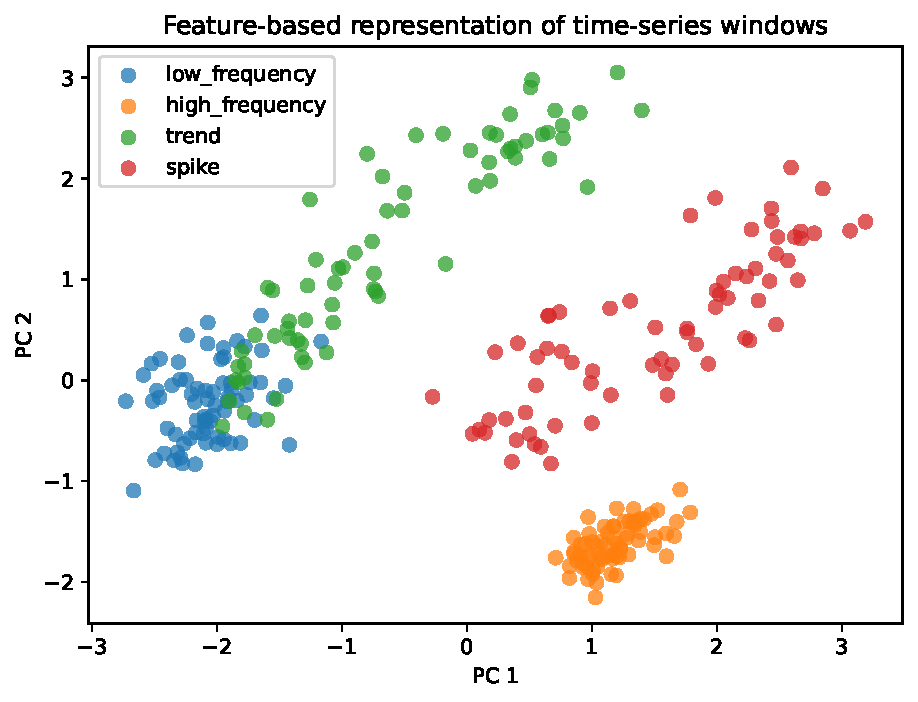
\includegraphics[keepaspectratio]{chapters/chapter-23-representation-learning-time-series_files/figure-pdf/ch23-python-feature-embedding-output-1.pdf}}

}

\caption{PCA embedding of handcrafted time-series features.}

\end{figure}%

The plot should not be interpreted as proof that PCA discovered the true
data-generating process. It only shows that the chosen features contain
enough information to separate the four synthetic families.

\section{23.12 Python example: PCA as a linear
autoencoder}\label{python-example-pca-as-a-linear-autoencoder}

PCA gives the best rank-\(k\) linear reconstruction in squared error.
This makes it a useful baseline for autoencoders.

\protect\phantomsection\label{ch23-python-pca-reconstruction}
\begin{Shaded}
\begin{Highlighting}[]
\ImportTok{from}\NormalTok{ sklearn.decomposition }\ImportTok{import}\NormalTok{ PCA}
\ImportTok{from}\NormalTok{ sklearn.metrics }\ImportTok{import}\NormalTok{ mean\_squared\_error}

\NormalTok{rng }\OperatorTok{=}\NormalTok{ np.random.default\_rng(}\DecValTok{11}\NormalTok{)}
\NormalTok{L }\OperatorTok{=} \DecValTok{100}
\NormalTok{normal }\OperatorTok{=}\NormalTok{ np.vstack([make\_window(}\StringTok{"low\_frequency"}\NormalTok{, L}\OperatorTok{=}\NormalTok{L, rng}\OperatorTok{=}\NormalTok{rng, noise}\OperatorTok{=}\FloatTok{0.20}\NormalTok{) }\ControlFlowTok{for}\NormalTok{ \_ }\KeywordTok{in} \BuiltInTok{range}\NormalTok{(}\DecValTok{250}\NormalTok{)])}
\NormalTok{spiky }\OperatorTok{=}\NormalTok{ np.vstack([make\_window(}\StringTok{"spike"}\NormalTok{, L}\OperatorTok{=}\NormalTok{L, rng}\OperatorTok{=}\NormalTok{rng, noise}\OperatorTok{=}\FloatTok{0.20}\NormalTok{) }\ControlFlowTok{for}\NormalTok{ \_ }\KeywordTok{in} \BuiltInTok{range}\NormalTok{(}\DecValTok{40}\NormalTok{)])}

\NormalTok{k }\OperatorTok{=} \DecValTok{5}
\NormalTok{pca }\OperatorTok{=}\NormalTok{ PCA(n\_components}\OperatorTok{=}\NormalTok{k, random\_state}\OperatorTok{=}\DecValTok{0}\NormalTok{)}
\NormalTok{pca.fit(normal)}

\NormalTok{normal\_hat }\OperatorTok{=}\NormalTok{ pca.inverse\_transform(pca.transform(normal))}
\NormalTok{spiky\_hat }\OperatorTok{=}\NormalTok{ pca.inverse\_transform(pca.transform(spiky))}

\NormalTok{normal\_err }\OperatorTok{=}\NormalTok{ np.mean((normal }\OperatorTok{{-}}\NormalTok{ normal\_hat)}\OperatorTok{**}\DecValTok{2}\NormalTok{, axis}\OperatorTok{=}\DecValTok{1}\NormalTok{)}
\NormalTok{spiky\_err }\OperatorTok{=}\NormalTok{ np.mean((spiky }\OperatorTok{{-}}\NormalTok{ spiky\_hat)}\OperatorTok{**}\DecValTok{2}\NormalTok{, axis}\OperatorTok{=}\DecValTok{1}\NormalTok{)}

\BuiltInTok{print}\NormalTok{(}\SpecialStringTok{f"Median normal reconstruction error: }\SpecialCharTok{\{}\NormalTok{np}\SpecialCharTok{.}\NormalTok{median(normal\_err)}\SpecialCharTok{:.4f\}}\SpecialStringTok{"}\NormalTok{)}
\BuiltInTok{print}\NormalTok{(}\SpecialStringTok{f"Median spiky reconstruction error:  }\SpecialCharTok{\{}\NormalTok{np}\SpecialCharTok{.}\NormalTok{median(spiky\_err)}\SpecialCharTok{:.4f\}}\SpecialStringTok{"}\NormalTok{)}

\NormalTok{example\_normal }\OperatorTok{=}\NormalTok{ normal[}\DecValTok{0}\NormalTok{]}
\NormalTok{example\_spiky }\OperatorTok{=}\NormalTok{ spiky[}\DecValTok{0}\NormalTok{]}
\NormalTok{example\_normal\_hat }\OperatorTok{=}\NormalTok{ pca.inverse\_transform(pca.transform(example\_normal.reshape(}\DecValTok{1}\NormalTok{, }\OperatorTok{{-}}\DecValTok{1}\NormalTok{)))[}\DecValTok{0}\NormalTok{]}
\NormalTok{example\_spiky\_hat }\OperatorTok{=}\NormalTok{ pca.inverse\_transform(pca.transform(example\_spiky.reshape(}\DecValTok{1}\NormalTok{, }\OperatorTok{{-}}\DecValTok{1}\NormalTok{)))[}\DecValTok{0}\NormalTok{]}

\NormalTok{plt.figure(figsize}\OperatorTok{=}\NormalTok{(}\DecValTok{8}\NormalTok{, }\DecValTok{4}\NormalTok{))}
\NormalTok{plt.plot(example\_normal, label}\OperatorTok{=}\StringTok{"normal window"}\NormalTok{)}
\NormalTok{plt.plot(example\_normal\_hat, label}\OperatorTok{=}\StringTok{"PCA reconstruction"}\NormalTok{)}
\NormalTok{plt.title(}\StringTok{"Normal window reconstruction"}\NormalTok{)}
\NormalTok{plt.legend()}
\NormalTok{plt.show()}

\NormalTok{plt.figure(figsize}\OperatorTok{=}\NormalTok{(}\DecValTok{8}\NormalTok{, }\DecValTok{4}\NormalTok{))}
\NormalTok{plt.plot(example\_spiky, label}\OperatorTok{=}\StringTok{"spiky window"}\NormalTok{)}
\NormalTok{plt.plot(example\_spiky\_hat, label}\OperatorTok{=}\StringTok{"PCA reconstruction"}\NormalTok{)}
\NormalTok{plt.title(}\StringTok{"Spiky window reconstruction"}\NormalTok{)}
\NormalTok{plt.legend()}
\NormalTok{plt.show()}
\end{Highlighting}
\end{Shaded}

\begin{verbatim}
Median normal reconstruction error: 0.0662
Median spiky reconstruction error:  0.9133
\end{verbatim}

\begin{figure}[H]

{\centering \pandocbounded{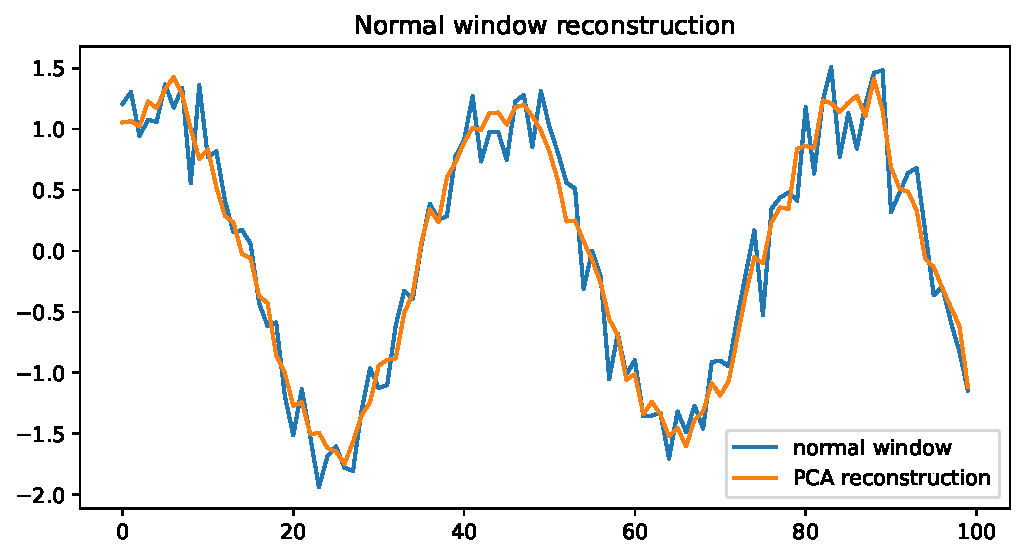
\includegraphics[keepaspectratio]{chapters/chapter-23-representation-learning-time-series_files/figure-pdf/ch23-python-pca-reconstruction-output-2.pdf}}

}

\caption{A low-dimensional PCA representation reconstructs smooth
windows better than spiky windows.}

\end{figure}%

\pandocbounded{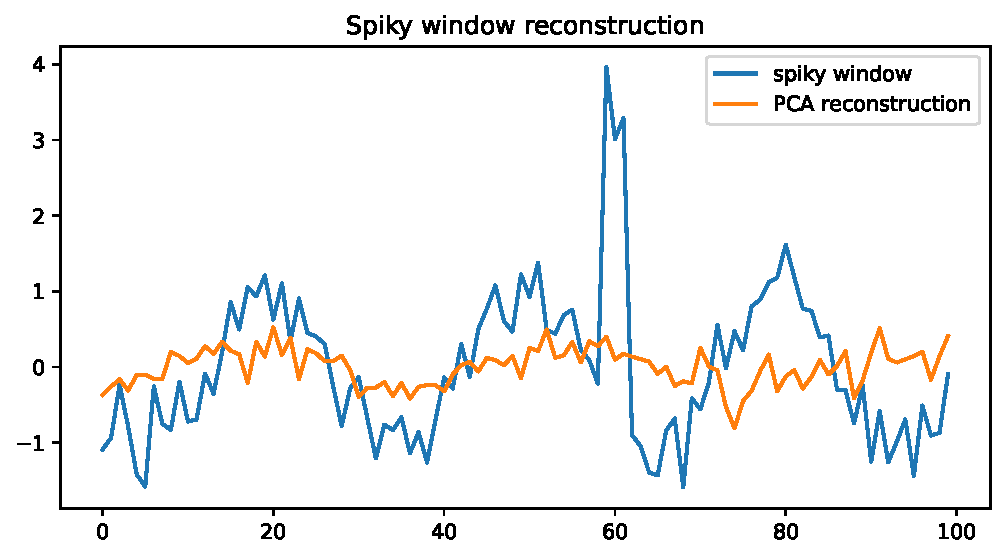
\includegraphics[keepaspectratio]{chapters/chapter-23-representation-learning-time-series_files/figure-pdf/ch23-python-pca-reconstruction-output-3.pdf}}

\section{23.13 Python example: a small neural
autoencoder}\label{python-example-a-small-neural-autoencoder}

The next example trains a small MLP autoencoder. This is not meant to be
a state-of-the-art model. It is a minimal representation-learning
template.

\begin{Shaded}
\begin{Highlighting}[]
\ImportTok{import}\NormalTok{ torch}
\ImportTok{from}\NormalTok{ torch }\ImportTok{import}\NormalTok{ nn}
\ImportTok{from}\NormalTok{ torch.utils.data }\ImportTok{import}\NormalTok{ TensorDataset, DataLoader}

\NormalTok{torch.set\_num\_threads(}\DecValTok{1}\NormalTok{)}
\NormalTok{torch.manual\_seed(}\DecValTok{0}\NormalTok{)}

\NormalTok{rng }\OperatorTok{=}\NormalTok{ np.random.default\_rng(}\DecValTok{21}\NormalTok{)}
\NormalTok{L }\OperatorTok{=} \DecValTok{80}
\NormalTok{train\_windows }\OperatorTok{=}\NormalTok{ np.vstack([}
\NormalTok{    make\_window(}\StringTok{"low\_frequency"}\NormalTok{, L}\OperatorTok{=}\NormalTok{L, rng}\OperatorTok{=}\NormalTok{rng, noise}\OperatorTok{=}\FloatTok{0.25}\NormalTok{)}
    \ControlFlowTok{for}\NormalTok{ \_ }\KeywordTok{in} \BuiltInTok{range}\NormalTok{(}\DecValTok{300}\NormalTok{)}
\NormalTok{]).astype(}\StringTok{"float32"}\NormalTok{)}

\NormalTok{tensor }\OperatorTok{=}\NormalTok{ torch.tensor(train\_windows)}
\NormalTok{loader }\OperatorTok{=}\NormalTok{ DataLoader(TensorDataset(tensor), batch\_size}\OperatorTok{=}\DecValTok{64}\NormalTok{, shuffle}\OperatorTok{=}\VariableTok{True}\NormalTok{)}

\KeywordTok{class}\NormalTok{ Autoencoder(nn.Module):}
    \KeywordTok{def} \FunctionTok{\_\_init\_\_}\NormalTok{(}\VariableTok{self}\NormalTok{, L, d):}
        \BuiltInTok{super}\NormalTok{().}\FunctionTok{\_\_init\_\_}\NormalTok{()}
        \VariableTok{self}\NormalTok{.encoder }\OperatorTok{=}\NormalTok{ nn.Sequential(}
\NormalTok{            nn.Linear(L, }\DecValTok{32}\NormalTok{),}
\NormalTok{            nn.ReLU(),}
\NormalTok{            nn.Linear(}\DecValTok{32}\NormalTok{, d)}
\NormalTok{        )}
        \VariableTok{self}\NormalTok{.decoder }\OperatorTok{=}\NormalTok{ nn.Sequential(}
\NormalTok{            nn.Linear(d, }\DecValTok{32}\NormalTok{),}
\NormalTok{            nn.ReLU(),}
\NormalTok{            nn.Linear(}\DecValTok{32}\NormalTok{, L)}
\NormalTok{        )}

    \KeywordTok{def}\NormalTok{ forward(}\VariableTok{self}\NormalTok{, x):}
\NormalTok{        z }\OperatorTok{=} \VariableTok{self}\NormalTok{.encoder(x)}
\NormalTok{        xhat }\OperatorTok{=} \VariableTok{self}\NormalTok{.decoder(z)}
        \ControlFlowTok{return}\NormalTok{ xhat, z}

\NormalTok{model }\OperatorTok{=}\NormalTok{ Autoencoder(L}\OperatorTok{=}\NormalTok{L, d}\OperatorTok{=}\DecValTok{4}\NormalTok{)}
\NormalTok{optimizer }\OperatorTok{=}\NormalTok{ torch.optim.Adam(model.parameters(), lr}\OperatorTok{=}\FloatTok{1e{-}3}\NormalTok{)}
\NormalTok{loss\_fn }\OperatorTok{=}\NormalTok{ nn.MSELoss()}
\NormalTok{losses }\OperatorTok{=}\NormalTok{ []}

\ControlFlowTok{for}\NormalTok{ epoch }\KeywordTok{in} \BuiltInTok{range}\NormalTok{(}\DecValTok{60}\NormalTok{):}
\NormalTok{    total }\OperatorTok{=} \FloatTok{0.0}
\NormalTok{    count }\OperatorTok{=} \DecValTok{0}
    \ControlFlowTok{for}\NormalTok{ (xb,) }\KeywordTok{in}\NormalTok{ loader:}
\NormalTok{        optimizer.zero\_grad()}
\NormalTok{        xhat, \_ }\OperatorTok{=}\NormalTok{ model(xb)}
\NormalTok{        loss }\OperatorTok{=}\NormalTok{ loss\_fn(xhat, xb)}
\NormalTok{        loss.backward()}
\NormalTok{        optimizer.step()}
\NormalTok{        total }\OperatorTok{+=}\NormalTok{ loss.item() }\OperatorTok{*}\NormalTok{ xb.shape[}\DecValTok{0}\NormalTok{]}
\NormalTok{        count }\OperatorTok{+=}\NormalTok{ xb.shape[}\DecValTok{0}\NormalTok{]}
\NormalTok{    losses.append(total }\OperatorTok{/}\NormalTok{ count)}

\NormalTok{plt.figure(figsize}\OperatorTok{=}\NormalTok{(}\DecValTok{7}\NormalTok{, }\DecValTok{4}\NormalTok{))}
\NormalTok{plt.plot(losses)}
\NormalTok{plt.xlabel(}\StringTok{"epoch"}\NormalTok{)}
\NormalTok{plt.ylabel(}\StringTok{"MSE reconstruction loss"}\NormalTok{)}
\NormalTok{plt.title(}\StringTok{"Autoencoder training loss"}\NormalTok{)}
\NormalTok{plt.show()}

\ControlFlowTok{with}\NormalTok{ torch.no\_grad():}
\NormalTok{    xhat, z }\OperatorTok{=}\NormalTok{ model(tensor[:}\DecValTok{5}\NormalTok{])}
\BuiltInTok{print}\NormalTok{(}\StringTok{"Latent representation shape:"}\NormalTok{, z.shape)}
\end{Highlighting}
\end{Shaded}

\begin{figure}[H]

{\centering \pandocbounded{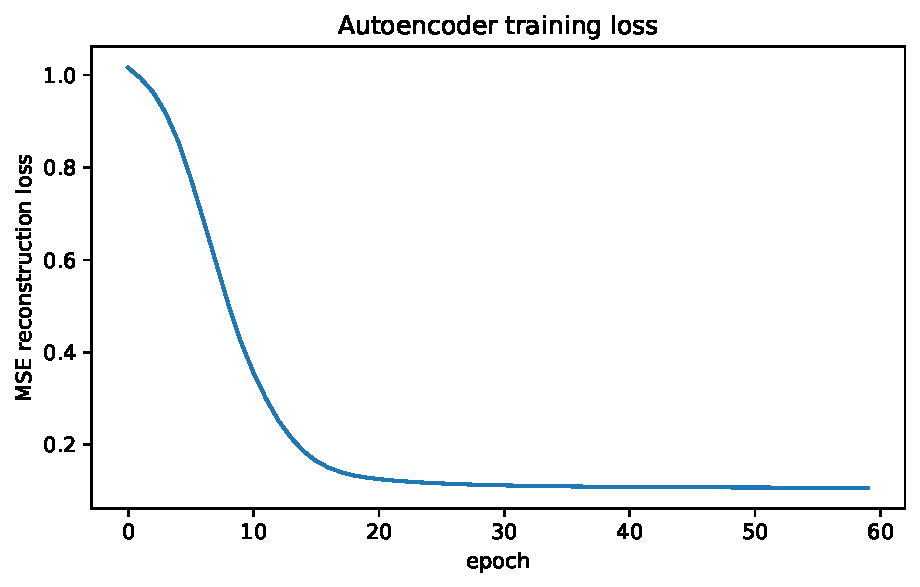
\includegraphics[keepaspectratio]{chapters/chapter-23-representation-learning-time-series_files/figure-pdf/ch23-python-mlp-autoencoder-output-1.pdf}}

}

\caption{Training loss for a small MLP autoencoder.}

\end{figure}%

\begin{verbatim}
Latent representation shape: torch.Size([5, 4])
\end{verbatim}

The tensor \texttt{z} contains the learned representation. A downstream
model could use \texttt{z} instead of the original \(L\)-dimensional
window.

\section{23.14 Python example: masked reconstruction pretext
task}\label{python-example-masked-reconstruction-pretext-task}

Masked reconstruction trains a model to infer missing parts from
context. Here is a simple non-neural demonstration of the idea.

\begin{Shaded}
\begin{Highlighting}[]
\NormalTok{rng }\OperatorTok{=}\NormalTok{ np.random.default\_rng(}\DecValTok{31}\NormalTok{)}
\NormalTok{L }\OperatorTok{=} \DecValTok{120}
\NormalTok{t }\OperatorTok{=}\NormalTok{ np.arange(L)}
\NormalTok{x }\OperatorTok{=}\NormalTok{ np.sin(}\DecValTok{2}\OperatorTok{*}\NormalTok{np.pi}\OperatorTok{*}\NormalTok{t}\OperatorTok{/}\DecValTok{35}\NormalTok{) }\OperatorTok{+} \FloatTok{0.35}\OperatorTok{*}\NormalTok{np.sin(}\DecValTok{2}\OperatorTok{*}\NormalTok{np.pi}\OperatorTok{*}\NormalTok{t}\OperatorTok{/}\DecValTok{9}\NormalTok{) }\OperatorTok{+} \FloatTok{0.15}\OperatorTok{*}\NormalTok{rng.normal(size}\OperatorTok{=}\NormalTok{L)}

\NormalTok{mask }\OperatorTok{=}\NormalTok{ np.zeros(L, dtype}\OperatorTok{=}\BuiltInTok{bool}\NormalTok{)}
\NormalTok{mask[}\DecValTok{45}\NormalTok{:}\DecValTok{65}\NormalTok{] }\OperatorTok{=} \VariableTok{True}
\NormalTok{observed\_t }\OperatorTok{=}\NormalTok{ t[}\OperatorTok{\textasciitilde{}}\NormalTok{mask]}
\NormalTok{observed\_x }\OperatorTok{=}\NormalTok{ x[}\OperatorTok{\textasciitilde{}}\NormalTok{mask]}

\CommentTok{\# A simple interpolation baseline for the masked block.}
\NormalTok{x\_recon }\OperatorTok{=}\NormalTok{ x.copy()}
\NormalTok{x\_recon[mask] }\OperatorTok{=}\NormalTok{ np.interp(t[mask], observed\_t, observed\_x)}

\NormalTok{masked\_mse }\OperatorTok{=}\NormalTok{ np.mean((x[mask] }\OperatorTok{{-}}\NormalTok{ x\_recon[mask])}\OperatorTok{**}\DecValTok{2}\NormalTok{)}
\BuiltInTok{print}\NormalTok{(}\SpecialStringTok{f"Masked{-}block reconstruction MSE: }\SpecialCharTok{\{}\NormalTok{masked\_mse}\SpecialCharTok{:.4f\}}\SpecialStringTok{"}\NormalTok{)}

\NormalTok{plt.figure(figsize}\OperatorTok{=}\NormalTok{(}\DecValTok{8}\NormalTok{, }\DecValTok{4}\NormalTok{))}
\NormalTok{plt.plot(t, x, label}\OperatorTok{=}\StringTok{"true sequence"}\NormalTok{)}
\NormalTok{plt.plot(t, x\_recon, label}\OperatorTok{=}\StringTok{"masked reconstruction"}\NormalTok{)}
\NormalTok{plt.scatter(t[mask], x[mask], label}\OperatorTok{=}\StringTok{"hidden values"}\NormalTok{)}
\NormalTok{plt.xlabel(}\StringTok{"time"}\NormalTok{)}
\NormalTok{plt.title(}\StringTok{"Self{-}supervised masked reconstruction task"}\NormalTok{)}
\NormalTok{plt.legend()}
\NormalTok{plt.show()}
\end{Highlighting}
\end{Shaded}

\begin{verbatim}
Masked-block reconstruction MSE: 0.3641
\end{verbatim}

\begin{figure}[H]

{\centering \pandocbounded{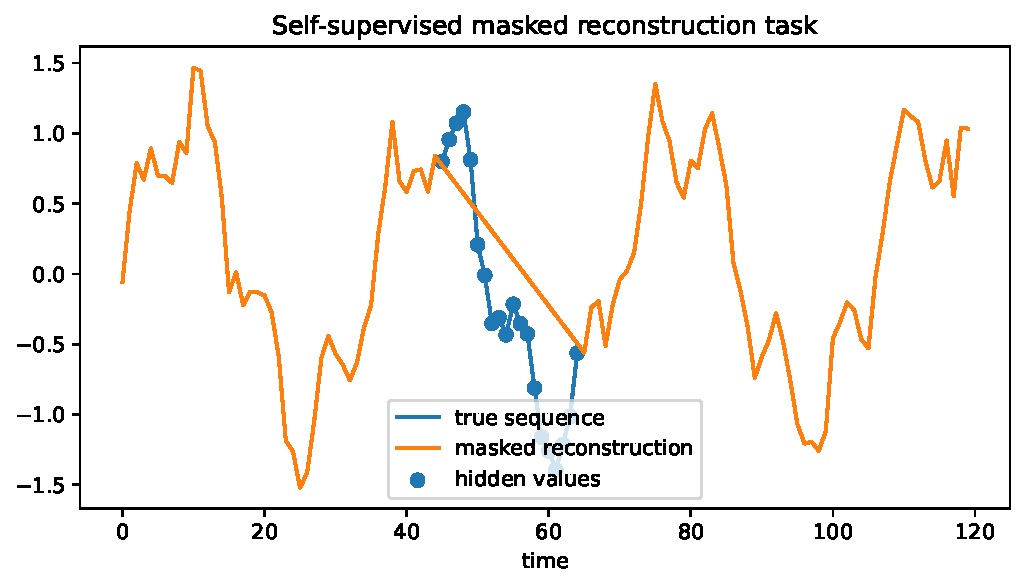
\includegraphics[keepaspectratio]{chapters/chapter-23-representation-learning-time-series_files/figure-pdf/ch23-python-masked-reconstruction-output-2.pdf}}

}

\caption{Masked reconstruction as a self-supervised pretext task.}

\end{figure}%

A neural masked-reconstruction model replaces interpolation with a
learned encoder-decoder, usually trained over many random masks.

\section{23.15 AI-assisted representation
critique}\label{ai-assisted-representation-critique}

\section{AI-assisted study box}\label{ai-assisted-study-box-2}

Ask an AI assistant to review a representation-learning pipeline.
Require the answer to address the following points:

\begin{enumerate}
\def\labelenumi{\arabic{enumi}.}
\tightlist
\item
  What is the input window \(X_i\) and what is the latent representation
  \(\mathbf z_i\)?
\item
  Is the representation trained supervised, unsupervised, or
  self-supervised?
\item
  What objective function is being minimized?
\item
  What downstream task is used to evaluate the representation?
\item
  Which preprocessing steps could leak test information?
\item
  What baseline representation should be compared against?
\item
  How should nearest neighbors in latent space be inspected?
\item
  What would constitute evidence that the representation learned only
  noise?
\end{enumerate}

Then verify the answer using code. Do not accept vague statements such
as ``the embedding captures temporal patterns'' unless the statement is
connected to a diagnostic, task metric, or visualization.

A useful prompt template is:

\begin{quote}
I am training a representation model for time-series windows. The
encoder maps \(L\) past observations to a \(d\)-dimensional latent
vector. Please audit the pipeline for leakage, propose baseline
representations, recommend diagnostics for latent-space quality, and
identify failure modes. Give concrete tests I can run in Python.
\end{quote}

\section{23.16 Common mistakes}\label{common-mistakes-22}

\begin{enumerate}
\def\labelenumi{\arabic{enumi}.}
\tightlist
\item
  \textbf{Using random train-test splits for overlapping windows.}
  Adjacent windows share most observations, so random splits can create
  severe leakage.
\item
  \textbf{Fitting PCA or scalers on the full dataset before splitting.}
  This uses test information in the representation.
\item
  \textbf{Judging an embedding only by a pretty two-dimensional plot.}
  Visualization is useful, but downstream validation is necessary.
\item
  \textbf{Confusing reconstruction with prediction.} Low reconstruction
  error does not imply good forecast performance.
\item
  \textbf{Using invalid augmentations.} An augmentation must preserve
  task-relevant structure.
\item
  \textbf{Ignoring baselines.} Handcrafted features and PCA are
  essential comparisons.
\item
  \textbf{Overcompressing.} If \(d\) is too small, important temporal
  information may be destroyed.
\item
  \textbf{Undercompressing.} If \(d\) is too large, the representation
  may memorize noise.
\item
  \textbf{Failing to inspect nearest neighbors.} If nearest neighbors
  look unrelated in the original time domain, the embedding geometry may
  be poor.
\end{enumerate}

\section{23.17 Exercises}\label{exercises-22}

\begin{enumerate}
\def\labelenumi{\arabic{enumi}.}
\tightlist
\item
  Let \(X\in\mathbb R^{N\times L}\) be a centered matrix of time-series
  windows. Show that the PCA reconstruction \(\widehat X=XV_dV_d^T\)
  minimizes squared reconstruction error among all rank-\(d\) linear
  projections.
\item
  Construct two different feature maps \(\Phi_1\) and \(\Phi_2\) for
  time-series windows. One should emphasize time-domain features and the
  other should emphasize frequency-domain features.
\item
  Simulate three classes of windows: low-frequency, high-frequency, and
  spiky. Compare PCA embeddings from raw windows and PCA embeddings from
  handcrafted features.
\item
  Train a small autoencoder on normal windows and evaluate
  reconstruction error on anomalous windows.
\item
  Design a contrastive-learning augmentation set for one of the
  following: electricity demand, ECG signals, stock returns, or climate
  data. Explain which augmentations are valid and which are invalid.
\item
  Suppose a representation is trained on the entire dataset and then
  used for forecasting evaluation. Explain precisely why this can leak
  information.
\item
  Use nearest-neighbor retrieval in latent space. For five query
  windows, plot their nearest neighbors and describe whether the latent
  geometry is meaningful.
\item
  Compare reconstruction error and downstream forecasting error as the
  latent dimension \(d\) changes.
\end{enumerate}

\section{23.18 Mini project}\label{mini-project-6}

Choose a real or simulated time-series dataset. Build three
representations:

\begin{enumerate}
\def\labelenumi{\arabic{enumi}.}
\tightlist
\item
  handcrafted features;
\item
  PCA or another linear embedding;
\item
  a neural autoencoder embedding.
\end{enumerate}

Evaluate the representations on at least one downstream task, such as
clustering, anomaly detection, sequence classification, or forecasting.
Your report should include:

\begin{itemize}
\tightlist
\item
  a clear definition of the input windows;
\item
  the representation dimension \(d\);
\item
  the training/validation/test split;
\item
  a leakage audit;
\item
  a two-dimensional visualization;
\item
  nearest-neighbor examples;
\item
  one downstream metric;
\item
  a comparison with a simple baseline;
\item
  a short discussion of failure modes.
\end{itemize}

\section{23.19 Checklist}\label{checklist-7}

Before moving to the next chapter, make sure you can answer the
following questions.

\begin{itemize}
\tightlist
\item
  What is the difference between a raw window and a latent
  representation?
\item
  What does an encoder do?
\item
  Why is PCA a linear representation-learning method?
\item
  What objective does an autoencoder minimize?
\item
  Why can reconstruction loss be useful for anomaly detection?
\item
  Why might reconstruction loss fail to measure downstream usefulness?
\item
  What is a masked reconstruction pretext task?
\item
  What is the role of positive and negative pairs in contrastive
  learning?
\item
  How can scaling, PCA, or autoencoder training leak test information?
\item
  How would you check whether nearest neighbors in latent space are
  meaningful?
\end{itemize}

\section{23.20 Further reading}\label{further-reading-4}

\begin{itemize}
\tightlist
\item
  Shumway and Stoffer, \emph{Time Series Analysis and Its Applications},
  for classical time-series structure and diagnostics.
\item
  Goodfellow, Bengio, and Courville, \emph{Deep Learning}, for
  autoencoders and representation learning.
\item
  Recent literature on self-supervised learning for time series,
  including masked modeling, contrastive predictive coding, and
  transformer-based sequence pretraining.
\end{itemize}

\chapter{Multivariate, Panel, and Hierarchical Time
Series}\label{multivariate-panel-and-hierarchical-time-series}

\textbf{Part VI. Deep Learning for Time Series and Sequence Data}\\
\textbf{Chapter goal:} extend time-series modeling from one sequence to
many related sequences. We study multivariate dependence, vector
autoregressions, exogenous predictors, panel/global forecasting,
hierarchical aggregation, forecast reconciliation, and leakage-aware
validation.

\section{Learning objectives}\label{learning-objectives-23}

After studying this chapter, you should be able to:

\begin{enumerate}
\def\labelenumi{\arabic{enumi}.}
\tightlist
\item
  distinguish univariate, multivariate, panel, and hierarchical
  time-series problems;
\item
  define vector mean functions, matrix autocovariances, and
  cross-correlations;
\item
  formulate, estimate, and forecast with vector autoregressive models;
\item
  interpret cross-lag effects, impulse responses, and Granger-predictive
  relationships carefully;
\item
  explain why global models can share information across related series;
\item
  write hierarchical time-series aggregation in matrix form;
\item
  diagnose incoherent base forecasts and reconcile them using projection
  methods;
\item
  design validation splits that avoid time leakage and cross-sectional
  leakage;
\item
  implement VAR estimation and simple hierarchical reconciliation in
  Python;
\item
  use AI tools to critique multivariate and hierarchical forecasting
  workflows while verifying the mathematics.
\end{enumerate}

\section{24.1 Why one time series is often not
enough}\label{why-one-time-series-is-often-not-enough}

Many real forecasting problems are not isolated univariate problems. A
university may forecast enrollments across programs, colleges, campuses,
and modalities. A retailer forecasts sales for many products and stores.
An energy system forecasts total demand, regional demand, and demand by
customer type. A biomedical device records several sensor channels at
once.

These settings introduce three kinds of structure.

\textbf{Multivariate time series.} At each time \(t\), we observe a
vector

\[
\mathbf y_t=(y_{1t},\ldots,y_{pt})^T\in\mathbb R^p.
\]

The components are observed at the same time points and may influence
one another dynamically.

\textbf{Panel time series.} We observe many related series indexed by
\(i=1,\ldots,m\):

\[
y_{i,t},\qquad t=1,\ldots,T_i.
\]

The series may not be aggregated versions of one another, but they share
patterns such as seasonality, calendar effects, or response to
covariates.

\textbf{Hierarchical time series.} Some series are sums of other series.
For example,

\[
y_{\text{Total},t}=y_{A,t}+y_{B,t}+y_{C,t}.
\]

A good forecasting system should not forecast the total as \(100\) while
the forecasted parts sum to \(115\). Such forecasts are
\textbf{incoherent}.

\begin{tcolorbox}[enhanced jigsaw, arc=.35mm, bottomrule=.15mm, bottomtitle=1mm, breakable, colback=white, colbacktitle=quarto-callout-note-color!10!white, colframe=quarto-callout-note-color-frame, coltitle=black, left=2mm, leftrule=.75mm, opacityback=0, opacitybacktitle=0.6, rightrule=.15mm, title=\textcolor{quarto-callout-note-color}{\faInfo}\hspace{0.5em}{Main lesson}, titlerule=0mm, toprule=.15mm, toptitle=1mm]

Classical univariate models explain temporal dependence within one
sequence. Modern forecasting systems also model dependence
\textbf{across variables}, \textbf{across related units}, and
\textbf{across aggregation levels}.

\end{tcolorbox}

\section{24.2 Vector-valued stationarity and
cross-dependence}\label{vector-valued-stationarity-and-cross-dependence}

Let \(\{\mathbf y_t\}\) be a \(p\)-dimensional time series. Its mean
vector is

\[
\boldsymbol\mu_t=E(\mathbf y_t).
\]

Its lag-\(h\) autocovariance matrix is

\[
\Gamma(h)=\operatorname{Cov}(\mathbf y_{t+h},\mathbf y_t)
=E\left[(\mathbf y_{t+h}-\boldsymbol\mu)(\mathbf y_t-\boldsymbol\mu)^T\right],
\]

when the process is weakly stationary. The \((i,j)\) entry of
\(\Gamma(h)\) is

\[
\Gamma_{ij}(h)=\operatorname{Cov}(y_{i,t+h},y_{j,t}).
\]

This quantity measures whether variable \(j\) at time \(t\) helps
linearly explain variable \(i\) at time \(t+h\).

A \(p\)-dimensional process is weakly stationary if:

\[
E(\mathbf y_t)=\boldsymbol\mu
\]

is constant and

\[
\operatorname{Cov}(\mathbf y_{t+h},\mathbf y_t)=\Gamma(h)
\]

depends only on \(h\), not on \(t\).

The matrix autocovariance satisfies

\[
\Gamma(-h)=\Gamma(h)^T.
\]

The lag-\(h\) cross-correlation between component \(i\) and component
\(j\) is

\[
\rho_{ij}(h)=
\frac{\Gamma_{ij}(h)}{\sqrt{\Gamma_{ii}(0)\Gamma_{jj}(0)}}.
\]

For \(h>0\), \(\rho_{ij}(h)\) relates \(y_{j,t}\) to \(y_{i,t+h}\).
Thus, the direction of the lag matters.

\begin{tcolorbox}[enhanced jigsaw, arc=.35mm, bottomrule=.15mm, bottomtitle=1mm, breakable, colback=white, colbacktitle=quarto-callout-warning-color!10!white, colframe=quarto-callout-warning-color-frame, coltitle=black, left=2mm, leftrule=.75mm, opacityback=0, opacitybacktitle=0.6, rightrule=.15mm, title=\textcolor{quarto-callout-warning-color}{\faExclamationTriangle}\hspace{0.5em}{Cross-correlation is not causal proof}, titlerule=0mm, toprule=.15mm, toptitle=1mm]

A large lagged cross-correlation can indicate predictive information, a
shared driver, seasonality, a trend artifact, or leakage. It should be
interpreted only after checking stationarity, calendar effects, and the
data-generating context.

\end{tcolorbox}

\section{24.3 Vector autoregression}\label{vector-autoregression}

A vector autoregression of order \(p\), written VAR(\(p\)), is

\[
\mathbf y_t=\mathbf c+A_1\mathbf y_{t-1}+A_2\mathbf y_{t-2}+\cdots+A_p\mathbf y_{t-p}+\boldsymbol\varepsilon_t,
\]

where

\[
\boldsymbol\varepsilon_t\sim WN_p(\mathbf 0,\Sigma_\varepsilon).
\]

Here \(A_k\in\mathbb R^{p\times p}\) is a matrix of lag-\(k\) effects.
The entry \((A_k)_{ij}\) measures the linear effect of variable \(j\) at
lag \(k\) on variable \(i\) at the current time.

For VAR(1),

\[
\mathbf y_t=\mathbf c+A\mathbf y_{t-1}+\boldsymbol\varepsilon_t.
\]

If all eigenvalues of \(A\) have modulus less than \(1\), then the
process is stable and has the causal representation

\[
\mathbf y_t=\boldsymbol\mu+\sum_{j=0}^{\infty}A^j\boldsymbol\varepsilon_{t-j},
\]

where

\[
\boldsymbol\mu=(I-A)^{-1}\mathbf c.
\]

This is the multivariate analogue of the AR(1) causal expansion

\[
y_t=\mu+\sum_{j=0}^{\infty}\phi^j\varepsilon_{t-j}.
\]

For VAR(\(p\)), stability is checked using the companion matrix

\[
\mathcal A=
\begin{bmatrix}
A_1&A_2&\cdots&A_{p-1}&A_p\\
I&0&\cdots&0&0\\
0&I&\cdots&0&0\\
\vdots&\vdots&\ddots&\vdots&\vdots\\
0&0&\cdots&I&0
\end{bmatrix}.
\]

The VAR(\(p\)) is stable if every eigenvalue of \(\mathcal A\) lies
inside the unit circle.

\section{24.4 Forecasting with a VAR
model}\label{forecasting-with-a-var-model}

For VAR(1), the one-step forecast from time \(t\) is

\[
\widehat{\mathbf y}_{t+1|t}=\widehat{\mathbf c}+\widehat A\mathbf y_t.
\]

The two-step forecast is obtained recursively:

\[
\widehat{\mathbf y}_{t+2|t}=\widehat{\mathbf c}+\widehat A\widehat{\mathbf y}_{t+1|t}.
\]

More generally,

\[
\widehat{\mathbf y}_{t+h|t}=\widehat{\mathbf c}+\widehat A\widehat{\mathbf y}_{t+h-1|t}.
\]

For VAR(\(p\)), the forecast uses the previous \(p\) vectors and
recursively substitutes forecasts for unknown future values.

Forecast uncertainty is also multivariate. If the parameters are treated
as known and the innovations have covariance matrix
\(\Sigma_\varepsilon\), then the \(h\)-step forecast-error covariance
for a stable VAR(1) is

\[
\operatorname{Var}(\mathbf y_{t+h}-\widehat{\mathbf y}_{t+h|t})
=\sum_{j=0}^{h-1}A^j\Sigma_\varepsilon(A^j)^T.
\]

The covariance matrix matters because forecast errors in different
variables may be correlated.

\section{24.5 Estimation by least
squares}\label{estimation-by-least-squares}

Suppose we fit a VAR(\(p\)) to observations
\(\mathbf y_1,\ldots,\mathbf y_T\). Define the response matrix

\[
Y=
\begin{bmatrix}
\mathbf y_{p+1}^T\\
\mathbf y_{p+2}^T\\
\vdots\\
\mathbf y_T^T
\end{bmatrix}
\in\mathbb R^{(T-p)\times p}.
\]

Define the design matrix

\[
X=
\begin{bmatrix}
1&\mathbf y_p^T&\mathbf y_{p-1}^T&\cdots&\mathbf y_1^T\\
1&\mathbf y_{p+1}^T&\mathbf y_p^T&\cdots&\mathbf y_2^T\\
\vdots&\vdots&\vdots&\ddots&\vdots\\
1&\mathbf y_{T-1}^T&\mathbf y_{T-2}^T&\cdots&\mathbf y_{T-p}^T
\end{bmatrix}.
\]

The VAR model can be written as the multivariate regression

\[
Y=XB+E.
\]

The least-squares estimator is

\[
\widehat B=(X^TX)^{-1}X^TY,
\]

assuming \(X^TX\) is invertible. This is equivalent to fitting one
regression equation for each component of \(\mathbf y_t\), using the
same lagged predictors.

The residual covariance is estimated by

\[
\widehat\Sigma_\varepsilon=\frac{1}{T-p-k}E^TE,
\]

where \(k=1+pp\) is the number of regression coefficients per equation
if an intercept is included.

\section{24.6 Cross-lag effects and impulse
responses}\label{cross-lag-effects-and-impulse-responses}

For VAR(1), a one-unit shock in component \(j\) at time \(t\) changes
the expected vector at time \(t+h\) by

\[
A^h\mathbf e_j,
\]

where \(\mathbf e_j\) is the \(j\)th standard basis vector. The sequence

\[
\mathbf e_j,
A\mathbf e_j,
A^2\mathbf e_j,
A^3\mathbf e_j,
\ldots
\]

is an impulse-response sequence.

Impulse responses help explain how a shock propagates through a
multivariate dynamic system. However, if innovation components are
contemporaneously correlated, then the interpretation of a shock depends
on how the shock is identified. Orthogonalized impulse responses require
additional assumptions, such as an ordering of variables.

\section{24.7 Granger-predictive
relationships}\label{granger-predictive-relationships}

Variable \(x_t\) is said to Granger-predict variable \(y_t\) if lagged
values of \(x_t\) improve prediction of \(y_t\) after accounting for
lagged values of \(y_t\) and other variables in the system.

A simple restricted model is

\[
y_t=\alpha+\sum_{k=1}^p a_k y_{t-k}+u_t.
\]

An unrestricted model is

\[
y_t=\alpha+\sum_{k=1}^p a_k y_{t-k}+\sum_{k=1}^p b_k x_{t-k}+v_t.
\]

If the coefficients \(b_1,\ldots,b_p\) are jointly useful for
prediction, then \(x\) Granger-predicts \(y\).

\begin{tcolorbox}[enhanced jigsaw, arc=.35mm, bottomrule=.15mm, bottomtitle=1mm, breakable, colback=white, colbacktitle=quarto-callout-important-color!10!white, colframe=quarto-callout-important-color-frame, coltitle=black, left=2mm, leftrule=.75mm, opacityback=0, opacitybacktitle=0.6, rightrule=.15mm, title=\textcolor{quarto-callout-important-color}{\faExclamation}\hspace{0.5em}{Terminology warning}, titlerule=0mm, toprule=.15mm, toptitle=1mm]

Granger prediction is about predictive improvement under a specified
information set. It is not the same as structural causality. Hidden
confounders, common seasonal drivers, data revisions, and
contemporaneous effects can create misleading Granger relationships.

\end{tcolorbox}

\section{24.8 Dynamic regression and exogenous
variables}\label{dynamic-regression-and-exogenous-variables}

Often we forecast a response series using lagged response values and
external predictors. A dynamic regression model may take the form

\[
y_t=\beta_0+\sum_{k=1}^{p}\phi_k y_{t-k}+\boldsymbol\beta^T\mathbf x_t+\varepsilon_t.
\]

If future covariates \(\mathbf x_{t+h}\) are known, such as calendar
indicators or scheduled prices, then they may be directly used in
forecasting. If they are unknown, they must themselves be forecasted or
scenario-defined.

For multivariate responses, a VAR with exogenous variables, often called
VARX, is

\[
\mathbf y_t=\mathbf c+\sum_{k=1}^p A_k\mathbf y_{t-k}+B\mathbf x_t+\boldsymbol\varepsilon_t.
\]

The key practical distinction is whether the future values of
\(\mathbf x_t\) are available at forecast time. Using future covariates
that would not be known in deployment is a form of leakage.

\section{24.9 Panel and global forecasting
models}\label{panel-and-global-forecasting-models}

In panel forecasting, we have many related series:

\[
y_{i,t},\qquad i=1,\ldots,m.
\]

A local strategy fits one model per series:

\[
y_{i,t}=f_i(y_{i,t-1},y_{i,t-2},\ldots)+\varepsilon_{i,t}.
\]

A global strategy fits a shared model:

\[
y_{i,t}=f_\theta(y_{i,t-1},\ldots,y_{i,t-L},\mathbf z_i,\mathbf x_{i,t})+\varepsilon_{i,t},
\]

where \(\mathbf z_i\) is a series identifier, static feature vector, or
learned embedding.

Global models can be helpful when individual series are short but the
panel is large. They borrow information across related series. However,
a global model can also transfer the wrong pattern if the series are
heterogeneous.

A simple pooled lag regression is

\[
y_{i,t}=\alpha_i+\sum_{k=1}^p \phi_k y_{i,t-k}+\boldsymbol\beta^T\mathbf x_{i,t}+\varepsilon_{i,t}.
\]

The intercept \(\alpha_i\) allows each series to have its own level,
while the lag coefficients \(\phi_k\) are shared.

\section{24.10 Hierarchical time series and aggregation
matrices}\label{hierarchical-time-series-and-aggregation-matrices}

Suppose a hierarchy has \(m\) bottom-level series collected in

\[
\mathbf b_t\in\mathbb R^m.
\]

All series in the hierarchy, including totals and intermediate
aggregates, are collected in

\[
\mathbf y_t\in\mathbb R^n.
\]

There is an aggregation matrix \(S\in\mathbb R^{n\times m}\) such that

\[
\mathbf y_t=S\mathbf b_t.
\]

For example, if the bottom series are \(A\), \(B\), and \(C\), and we
include the total, then

\[
\mathbf y_t=\begin{bmatrix}
\text{Total}_t\\A_t\\B_t\\C_t
\end{bmatrix},
\qquad
S=
\begin{bmatrix}
1&1&1\\
1&0&0\\
0&1&0\\
0&0&1
\end{bmatrix},
\qquad
\mathbf b_t=\begin{bmatrix}A_t\\B_t\\C_t\end{bmatrix}.
\]

A forecast vector \(\widehat{\mathbf y}_{t+h}\) is coherent if it
belongs to the column space of \(S\):

\[
\widehat{\mathbf y}_{t+h}=S\widehat{\mathbf b}_{t+h}
\]

for some bottom-level forecast \(\widehat{\mathbf b}_{t+h}\).

If we independently forecast all nodes in the hierarchy, we usually get
incoherent forecasts:

\[
\widehat y_{\text{Total},t+h}\neq
\widehat y_{A,t+h}+\widehat y_{B,t+h}+\widehat y_{C,t+h}.
\]

\section{24.11 Forecast reconciliation}\label{forecast-reconciliation}

Let \(\widehat{\mathbf y}\) be an incoherent vector of base forecasts
for all hierarchy nodes. Reconciliation replaces it with a coherent
forecast

\[
\widetilde{\mathbf y}=S\widetilde{\mathbf b}.
\]

One simple method is \textbf{bottom-up reconciliation}. Forecast the
bottom-level series and then aggregate:

\[
\widetilde{\mathbf y}=S\widehat{\mathbf b}.
\]

This is coherent but ignores information in the independently forecasted
aggregate series.

A projection-based method finds the coherent vector closest to the base
forecast:

\[
\widetilde{\mathbf y}
=S(S^TS)^{-1}S^T\widehat{\mathbf y}.
\]

More generally, weighted least-squares reconciliation uses a positive
definite weight matrix \(W\):

\[
\widetilde{\mathbf y}
=S(S^TW^{-1}S)^{-1}S^TW^{-1}\widehat{\mathbf y}.
\]

If \(W\) estimates the covariance matrix of base forecast errors, this
is the foundation of MinT-style reconciliation. The intuition is that
unreliable base forecasts should receive less weight.

\section{24.12 Interactive module: VAR coupling
explorer}\label{interactive-module-var-coupling-explorer}

This module shows how cross-lag coefficients change the behavior of a
two-dimensional VAR(1):

\[
\begin{bmatrix}y_{1,t}\\y_{2,t}\end{bmatrix}
=
\begin{bmatrix}a_{11}&a_{12}\\a_{21}&a_{22}\end{bmatrix}
\begin{bmatrix}y_{1,t-1}\\y_{2,t-1}\end{bmatrix}
+\boldsymbol\varepsilon_t.
\]

The spectral radius \(\rho(A)\) determines stability for VAR(1). If
\(\rho(A)<1\), shocks decay. If \(\rho(A)>1\), the system can become
explosive.

Interactive Module: VAR(1) Coupling Explorer

Adjust own-lag and cross-lag coefficients. The plot shows simulated
paths and impulse responses. Stability is determined by the eigenvalues
of the coefficient matrix.

Own-lag \(a_{11}\):
\protect\phantomsection\label{ch24_var_a11_value}{0.60}

Own-lag \(a_{22}\):
\protect\phantomsection\label{ch24_var_a22_value}{0.40}

Cross-lag \(a_{12}\), from series 2 to series 1:
\protect\phantomsection\label{ch24_var_a12_value}{0.25}

Cross-lag \(a_{21}\), from series 1 to series 2:
\protect\phantomsection\label{ch24_var_a21_value}{0.10}

\protect\phantomsection\label{ch24_var_series_plot}

\protect\phantomsection\label{ch24_var_irf_plot}

\section{24.13 Interactive module: hierarchical
reconciliation}\label{interactive-module-hierarchical-reconciliation}

This module compares incoherent base forecasts with coherent reconciled
forecasts. The hierarchy is

\[
\text{Total}=A+B+C.
\]

The base forecast may violate this identity. Reconciliation projects the
base forecast onto the coherent subspace.

Interactive Module: Forecast Reconciliation

Move the base forecasts. The reconciled forecast is the ordinary
least-squares projection onto the coherent hierarchy Total = A + B + C.

Base total forecast:
\protect\phantomsection\label{ch24_rec_total_value}{125}

Base forecast A: \protect\phantomsection\label{ch24_rec_a_value}{45}

Base forecast B: \protect\phantomsection\label{ch24_rec_b_value}{35}

Base forecast C: \protect\phantomsection\label{ch24_rec_c_value}{30}

\protect\phantomsection\label{ch24_reconciliation_plot}

\section{24.14 Python example: simulating and estimating a
VAR(1)}\label{python-example-simulating-and-estimating-a-var1}

The next example simulates a stable two-dimensional VAR(1), estimates
the coefficient matrix by least squares, and produces recursive
forecasts.

\begin{Shaded}
\begin{Highlighting}[]
\ImportTok{import}\NormalTok{ numpy }\ImportTok{as}\NormalTok{ np}
\ImportTok{import}\NormalTok{ matplotlib.pyplot }\ImportTok{as}\NormalTok{ plt}

\NormalTok{rng }\OperatorTok{=}\NormalTok{ np.random.default\_rng(}\DecValTok{7339}\NormalTok{)}
\NormalTok{T }\OperatorTok{=} \DecValTok{240}
\NormalTok{A\_true }\OperatorTok{=}\NormalTok{ np.array([[}\FloatTok{0.65}\NormalTok{, }\FloatTok{0.25}\NormalTok{],}
\NormalTok{                   [}\FloatTok{0.10}\NormalTok{, }\FloatTok{0.45}\NormalTok{]])}
\NormalTok{c\_true }\OperatorTok{=}\NormalTok{ np.array([}\FloatTok{0.2}\NormalTok{, }\OperatorTok{{-}}\FloatTok{0.1}\NormalTok{])}
\NormalTok{Sigma }\OperatorTok{=}\NormalTok{ np.array([[}\FloatTok{1.00}\NormalTok{, }\FloatTok{0.35}\NormalTok{],}
\NormalTok{                  [}\FloatTok{0.35}\NormalTok{, }\FloatTok{0.80}\NormalTok{]])}

\NormalTok{Y }\OperatorTok{=}\NormalTok{ np.zeros((T, }\DecValTok{2}\NormalTok{))}
\NormalTok{noise }\OperatorTok{=}\NormalTok{ rng.multivariate\_normal(np.zeros(}\DecValTok{2}\NormalTok{), Sigma, size}\OperatorTok{=}\NormalTok{T)}
\ControlFlowTok{for}\NormalTok{ t }\KeywordTok{in} \BuiltInTok{range}\NormalTok{(}\DecValTok{1}\NormalTok{, T):}
\NormalTok{    Y[t] }\OperatorTok{=}\NormalTok{ c\_true }\OperatorTok{+}\NormalTok{ A\_true }\OperatorTok{@}\NormalTok{ Y[t}\OperatorTok{{-}}\DecValTok{1}\NormalTok{] }\OperatorTok{+}\NormalTok{ noise[t]}

\CommentTok{\# Estimate VAR(1): Y\_t = c + A Y\_\{t{-}1\} + eps\_t.}
\NormalTok{X }\OperatorTok{=}\NormalTok{ np.column\_stack([np.ones(T}\OperatorTok{{-}}\DecValTok{1}\NormalTok{), Y[:}\OperatorTok{{-}}\DecValTok{1}\NormalTok{]])}
\NormalTok{Y\_response }\OperatorTok{=}\NormalTok{ Y[}\DecValTok{1}\NormalTok{:]}
\NormalTok{B\_hat }\OperatorTok{=}\NormalTok{ np.linalg.lstsq(X, Y\_response, rcond}\OperatorTok{=}\VariableTok{None}\NormalTok{)[}\DecValTok{0}\NormalTok{]}
\NormalTok{c\_hat }\OperatorTok{=}\NormalTok{ B\_hat[}\DecValTok{0}\NormalTok{]}
\NormalTok{A\_hat }\OperatorTok{=}\NormalTok{ B\_hat[}\DecValTok{1}\NormalTok{:].T}

\BuiltInTok{print}\NormalTok{(}\StringTok{"Estimated intercept:"}\NormalTok{, np.}\BuiltInTok{round}\NormalTok{(c\_hat, }\DecValTok{3}\NormalTok{))}
\BuiltInTok{print}\NormalTok{(}\StringTok{"Estimated A:"}\NormalTok{)}
\BuiltInTok{print}\NormalTok{(np.}\BuiltInTok{round}\NormalTok{(A\_hat, }\DecValTok{3}\NormalTok{))}
\BuiltInTok{print}\NormalTok{(}\StringTok{"Eigenvalues of A\_hat:"}\NormalTok{, np.}\BuiltInTok{round}\NormalTok{(np.linalg.eigvals(A\_hat), }\DecValTok{3}\NormalTok{))}

\CommentTok{\# Forecast from the last observation.}
\NormalTok{H }\OperatorTok{=} \DecValTok{24}
\NormalTok{forecast }\OperatorTok{=}\NormalTok{ np.zeros((H, }\DecValTok{2}\NormalTok{))}
\NormalTok{current }\OperatorTok{=}\NormalTok{ Y[}\OperatorTok{{-}}\DecValTok{1}\NormalTok{]}
\ControlFlowTok{for}\NormalTok{ h }\KeywordTok{in} \BuiltInTok{range}\NormalTok{(H):}
\NormalTok{    current }\OperatorTok{=}\NormalTok{ c\_hat }\OperatorTok{+}\NormalTok{ A\_hat }\OperatorTok{@}\NormalTok{ current}
\NormalTok{    forecast[h] }\OperatorTok{=}\NormalTok{ current}

\NormalTok{fig, ax }\OperatorTok{=}\NormalTok{ plt.subplots(figsize}\OperatorTok{=}\NormalTok{(}\DecValTok{8}\NormalTok{, }\DecValTok{4}\NormalTok{))}
\NormalTok{time }\OperatorTok{=}\NormalTok{ np.arange(T)}
\NormalTok{future }\OperatorTok{=}\NormalTok{ np.arange(T, T }\OperatorTok{+}\NormalTok{ H)}
\NormalTok{ax.plot(time, Y[:, }\DecValTok{0}\NormalTok{], label}\OperatorTok{=}\StringTok{"series 1"}\NormalTok{)}
\NormalTok{ax.plot(time, Y[:, }\DecValTok{1}\NormalTok{], label}\OperatorTok{=}\StringTok{"series 2"}\NormalTok{)}
\NormalTok{ax.plot(future, forecast[:, }\DecValTok{0}\NormalTok{], }\StringTok{"{-}{-}"}\NormalTok{, label}\OperatorTok{=}\StringTok{"forecast 1"}\NormalTok{)}
\NormalTok{ax.plot(future, forecast[:, }\DecValTok{1}\NormalTok{], }\StringTok{"{-}{-}"}\NormalTok{, label}\OperatorTok{=}\StringTok{"forecast 2"}\NormalTok{)}
\NormalTok{ax.axvline(T }\OperatorTok{{-}} \DecValTok{1}\NormalTok{, linestyle}\OperatorTok{=}\StringTok{":"}\NormalTok{)}
\NormalTok{ax.set\_xlabel(}\StringTok{"time"}\NormalTok{)}
\NormalTok{ax.set\_ylabel(}\StringTok{"value"}\NormalTok{)}
\NormalTok{ax.set\_title(}\StringTok{"VAR(1) simulation and recursive forecast"}\NormalTok{)}
\NormalTok{ax.legend()}
\NormalTok{plt.show()}
\end{Highlighting}
\end{Shaded}

\begin{verbatim}
Estimated intercept: [ 0.196 -0.02 ]
Estimated A:
[[0.619 0.246]
 [0.018 0.499]]
Eigenvalues of A_hat: [0.648 0.47 ]
\end{verbatim}

\begin{figure}[H]

{\centering \pandocbounded{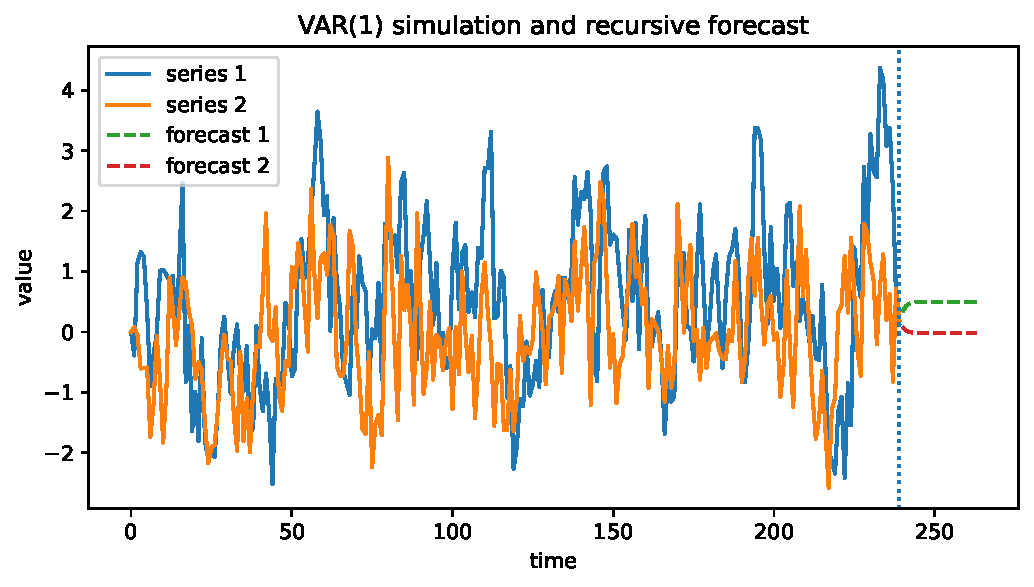
\includegraphics[keepaspectratio]{chapters/chapter-24-multivariate-panel-hierarchical_files/figure-pdf/ch24-python-var-estimation-output-2.pdf}}

}

\caption{Simulated bivariate VAR(1) series and recursive forecasts.}

\end{figure}%

\section{24.15 Python example: impulse
responses}\label{python-example-impulse-responses}

For a VAR(1), the response after \(h\) steps to a shock \(\mathbf s\) is
\(A^h\mathbf s\).

\begin{Shaded}
\begin{Highlighting}[]
\NormalTok{H }\OperatorTok{=} \DecValTok{25}
\NormalTok{shock }\OperatorTok{=}\NormalTok{ np.array([}\FloatTok{1.0}\NormalTok{, }\FloatTok{0.0}\NormalTok{])}
\NormalTok{responses }\OperatorTok{=}\NormalTok{ []}
\NormalTok{Ah }\OperatorTok{=}\NormalTok{ np.eye(}\DecValTok{2}\NormalTok{)}
\ControlFlowTok{for}\NormalTok{ h }\KeywordTok{in} \BuiltInTok{range}\NormalTok{(H):}
\NormalTok{    responses.append(Ah }\OperatorTok{@}\NormalTok{ shock)}
\NormalTok{    Ah }\OperatorTok{=}\NormalTok{ A\_hat }\OperatorTok{@}\NormalTok{ Ah}
\NormalTok{responses }\OperatorTok{=}\NormalTok{ np.array(responses)}

\NormalTok{fig, ax }\OperatorTok{=}\NormalTok{ plt.subplots(figsize}\OperatorTok{=}\NormalTok{(}\DecValTok{7}\NormalTok{, }\DecValTok{4}\NormalTok{))}
\NormalTok{ax.plot(np.arange(H), responses[:, }\DecValTok{0}\NormalTok{], marker}\OperatorTok{=}\StringTok{"o"}\NormalTok{, label}\OperatorTok{=}\StringTok{"response of series 1"}\NormalTok{)}
\NormalTok{ax.plot(np.arange(H), responses[:, }\DecValTok{1}\NormalTok{], marker}\OperatorTok{=}\StringTok{"o"}\NormalTok{, label}\OperatorTok{=}\StringTok{"response of series 2"}\NormalTok{)}
\NormalTok{ax.axhline(}\DecValTok{0}\NormalTok{, linewidth}\OperatorTok{=}\DecValTok{1}\NormalTok{)}
\NormalTok{ax.set\_xlabel(}\StringTok{"horizon"}\NormalTok{)}
\NormalTok{ax.set\_ylabel(}\StringTok{"response"}\NormalTok{)}
\NormalTok{ax.set\_title(}\StringTok{"Estimated impulse response to a shock in series 1"}\NormalTok{)}
\NormalTok{ax.legend()}
\NormalTok{plt.show()}
\end{Highlighting}
\end{Shaded}

\begin{figure}[H]

{\centering \pandocbounded{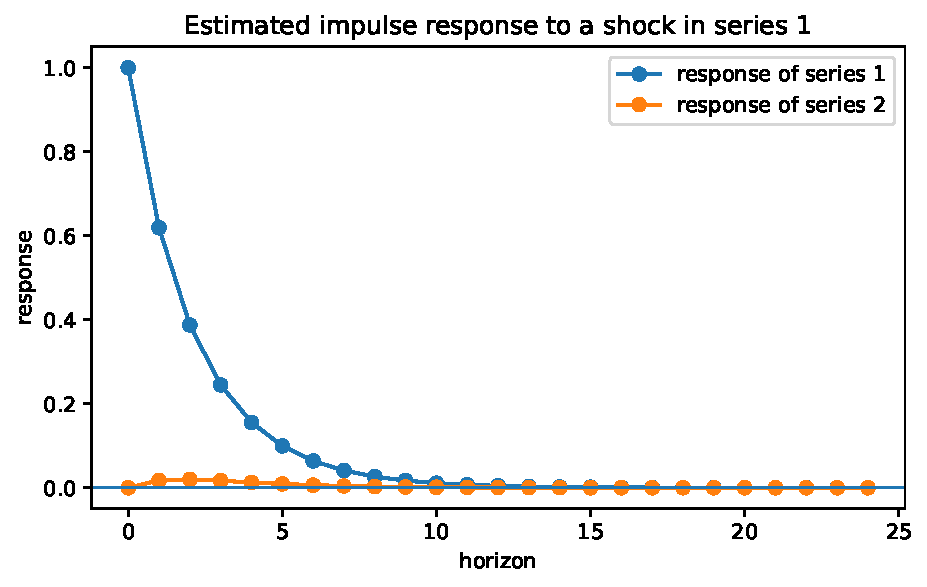
\includegraphics[keepaspectratio]{chapters/chapter-24-multivariate-panel-hierarchical_files/figure-pdf/ch24-python-impulse-response-output-1.pdf}}

}

\caption{Impulse responses from a shock to the first component.}

\end{figure}%

\section{24.16 Python example: hierarchical
reconciliation}\label{python-example-hierarchical-reconciliation}

The next example reconciles forecasts for a hierarchy with one total and
three bottom-level series.

\begin{Shaded}
\begin{Highlighting}[]
\ImportTok{import}\NormalTok{ numpy }\ImportTok{as}\NormalTok{ np}
\ImportTok{import}\NormalTok{ matplotlib.pyplot }\ImportTok{as}\NormalTok{ plt}

\CommentTok{\# y = [Total, A, B, C]\^{}T = S b, where b = [A, B, C]\^{}T.}
\NormalTok{S }\OperatorTok{=}\NormalTok{ np.array([[}\DecValTok{1}\NormalTok{, }\DecValTok{1}\NormalTok{, }\DecValTok{1}\NormalTok{],}
\NormalTok{              [}\DecValTok{1}\NormalTok{, }\DecValTok{0}\NormalTok{, }\DecValTok{0}\NormalTok{],}
\NormalTok{              [}\DecValTok{0}\NormalTok{, }\DecValTok{1}\NormalTok{, }\DecValTok{0}\NormalTok{],}
\NormalTok{              [}\DecValTok{0}\NormalTok{, }\DecValTok{0}\NormalTok{, }\DecValTok{1}\NormalTok{]], dtype}\OperatorTok{=}\BuiltInTok{float}\NormalTok{)}

\NormalTok{base }\OperatorTok{=}\NormalTok{ np.array([}\FloatTok{125.0}\NormalTok{, }\FloatTok{45.0}\NormalTok{, }\FloatTok{35.0}\NormalTok{, }\FloatTok{30.0}\NormalTok{])}
\BuiltInTok{print}\NormalTok{(}\StringTok{"Base total:"}\NormalTok{, base[}\DecValTok{0}\NormalTok{])}
\BuiltInTok{print}\NormalTok{(}\StringTok{"Sum of base bottom forecasts:"}\NormalTok{, base[}\DecValTok{1}\NormalTok{:].}\BuiltInTok{sum}\NormalTok{())}

\CommentTok{\# OLS reconciliation: project base forecast onto the coherent column space of S.}
\NormalTok{P }\OperatorTok{=}\NormalTok{ S }\OperatorTok{@}\NormalTok{ np.linalg.inv(S.T }\OperatorTok{@}\NormalTok{ S) }\OperatorTok{@}\NormalTok{ S.T}
\NormalTok{reconciled }\OperatorTok{=}\NormalTok{ P }\OperatorTok{@}\NormalTok{ base}

\BuiltInTok{print}\NormalTok{(}\StringTok{"Reconciled forecasts:"}\NormalTok{, np.}\BuiltInTok{round}\NormalTok{(reconciled, }\DecValTok{2}\NormalTok{))}
\BuiltInTok{print}\NormalTok{(}\StringTok{"Reconciled total:"}\NormalTok{, }\BuiltInTok{round}\NormalTok{(reconciled[}\DecValTok{0}\NormalTok{], }\DecValTok{2}\NormalTok{))}
\BuiltInTok{print}\NormalTok{(}\StringTok{"Sum of reconciled bottom forecasts:"}\NormalTok{, }\BuiltInTok{round}\NormalTok{(reconciled[}\DecValTok{1}\NormalTok{:].}\BuiltInTok{sum}\NormalTok{(), }\DecValTok{2}\NormalTok{))}

\NormalTok{labels }\OperatorTok{=}\NormalTok{ [}\StringTok{"Total"}\NormalTok{, }\StringTok{"A"}\NormalTok{, }\StringTok{"B"}\NormalTok{, }\StringTok{"C"}\NormalTok{]}
\NormalTok{x }\OperatorTok{=}\NormalTok{ np.arange(}\BuiltInTok{len}\NormalTok{(labels))}
\NormalTok{width }\OperatorTok{=} \FloatTok{0.35}
\NormalTok{fig, ax }\OperatorTok{=}\NormalTok{ plt.subplots(figsize}\OperatorTok{=}\NormalTok{(}\DecValTok{7}\NormalTok{, }\DecValTok{4}\NormalTok{))}
\NormalTok{ax.bar(x }\OperatorTok{{-}}\NormalTok{ width}\OperatorTok{/}\DecValTok{2}\NormalTok{, base, width, label}\OperatorTok{=}\StringTok{"base"}\NormalTok{)}
\NormalTok{ax.bar(x }\OperatorTok{+}\NormalTok{ width}\OperatorTok{/}\DecValTok{2}\NormalTok{, reconciled, width, label}\OperatorTok{=}\StringTok{"reconciled"}\NormalTok{)}
\NormalTok{ax.set\_xticks(x)}
\NormalTok{ax.set\_xticklabels(labels)}
\NormalTok{ax.set\_ylabel(}\StringTok{"forecast"}\NormalTok{)}
\NormalTok{ax.set\_title(}\StringTok{"Forecast reconciliation"}\NormalTok{)}
\NormalTok{ax.legend()}
\NormalTok{plt.show()}
\end{Highlighting}
\end{Shaded}

\begin{verbatim}
Base total: 125.0
Sum of base bottom forecasts: 110.0
Reconciled forecasts: [121.25  48.75  38.75  33.75]
Reconciled total: 121.25
Sum of reconciled bottom forecasts: 121.25
\end{verbatim}

\begin{figure}[H]

{\centering \pandocbounded{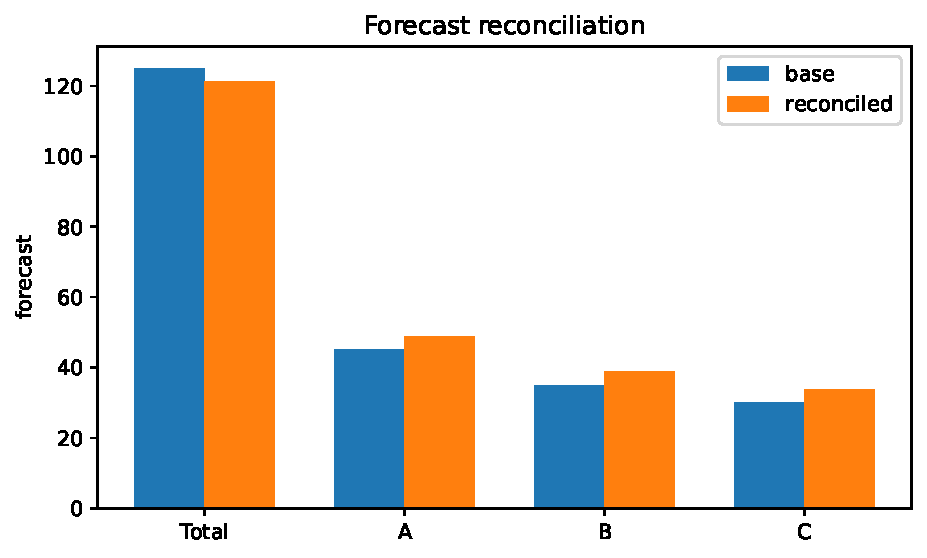
\includegraphics[keepaspectratio]{chapters/chapter-24-multivariate-panel-hierarchical_files/figure-pdf/ch24-python-hierarchical-reconciliation-output-2.pdf}}

}

\caption{Base forecasts and reconciled forecasts for a small hierarchy.}

\end{figure}%

\section{24.17 Python example: pooled lag model for panel
data}\label{python-example-pooled-lag-model-for-panel-data}

This example turns many related series into one supervised-learning
table. The model shares lag coefficients across series but allows
different intercepts through series indicators.

\begin{Shaded}
\begin{Highlighting}[]
\ImportTok{import}\NormalTok{ numpy }\ImportTok{as}\NormalTok{ np}
\ImportTok{import}\NormalTok{ pandas }\ImportTok{as}\NormalTok{ pd}
\ImportTok{import}\NormalTok{ matplotlib.pyplot }\ImportTok{as}\NormalTok{ plt}
\ImportTok{from}\NormalTok{ sklearn.linear\_model }\ImportTok{import}\NormalTok{ Ridge}
\ImportTok{from}\NormalTok{ sklearn.preprocessing }\ImportTok{import}\NormalTok{ OneHotEncoder}
\ImportTok{from}\NormalTok{ sklearn.compose }\ImportTok{import}\NormalTok{ ColumnTransformer}
\ImportTok{from}\NormalTok{ sklearn.pipeline }\ImportTok{import}\NormalTok{ Pipeline}
\ImportTok{from}\NormalTok{ sklearn.metrics }\ImportTok{import}\NormalTok{ mean\_squared\_error}

\NormalTok{rng }\OperatorTok{=}\NormalTok{ np.random.default\_rng(}\DecValTok{24}\NormalTok{)}
\NormalTok{m }\OperatorTok{=} \DecValTok{8}
\NormalTok{T }\OperatorTok{=} \DecValTok{120}
\NormalTok{rows }\OperatorTok{=}\NormalTok{ []}
\ControlFlowTok{for}\NormalTok{ i }\KeywordTok{in} \BuiltInTok{range}\NormalTok{(m):}
\NormalTok{    level }\OperatorTok{=}\NormalTok{ rng.normal(}\DecValTok{10}\NormalTok{, }\DecValTok{2}\NormalTok{)}
\NormalTok{    amp }\OperatorTok{=}\NormalTok{ rng.uniform(}\FloatTok{1.0}\NormalTok{, }\FloatTok{3.0}\NormalTok{)}
\NormalTok{    phi }\OperatorTok{=}\NormalTok{ rng.uniform(}\FloatTok{0.35}\NormalTok{, }\FloatTok{0.70}\NormalTok{)}
\NormalTok{    y }\OperatorTok{=}\NormalTok{ np.zeros(T)}
\NormalTok{    eps }\OperatorTok{=}\NormalTok{ rng.normal(}\DecValTok{0}\NormalTok{, }\FloatTok{0.8}\NormalTok{, T)}
    \ControlFlowTok{for}\NormalTok{ t }\KeywordTok{in} \BuiltInTok{range}\NormalTok{(}\DecValTok{1}\NormalTok{, T):}
\NormalTok{        seasonal }\OperatorTok{=}\NormalTok{ amp }\OperatorTok{*}\NormalTok{ np.sin(}\DecValTok{2}\OperatorTok{*}\NormalTok{np.pi}\OperatorTok{*}\NormalTok{t}\OperatorTok{/}\DecValTok{12} \OperatorTok{+} \FloatTok{0.4}\OperatorTok{*}\NormalTok{i)}
\NormalTok{        y[t] }\OperatorTok{=}\NormalTok{ level }\OperatorTok{+}\NormalTok{ phi}\OperatorTok{*}\NormalTok{(y[t}\OperatorTok{{-}}\DecValTok{1}\NormalTok{] }\OperatorTok{{-}}\NormalTok{ level) }\OperatorTok{+}\NormalTok{ seasonal }\OperatorTok{+}\NormalTok{ eps[t]}
    \ControlFlowTok{for}\NormalTok{ t }\KeywordTok{in} \BuiltInTok{range}\NormalTok{(}\DecValTok{2}\NormalTok{, T):}
\NormalTok{        rows.append(\{}\StringTok{"series"}\NormalTok{: }\SpecialStringTok{f"S}\SpecialCharTok{\{}\NormalTok{i}\SpecialCharTok{\}}\SpecialStringTok{"}\NormalTok{, }\StringTok{"time"}\NormalTok{: t, }\StringTok{"y"}\NormalTok{: y[t], }\StringTok{"lag1"}\NormalTok{: y[t}\OperatorTok{{-}}\DecValTok{1}\NormalTok{], }\StringTok{"lag2"}\NormalTok{: y[t}\OperatorTok{{-}}\DecValTok{2}\NormalTok{], }\StringTok{"month"}\NormalTok{: t }\OperatorTok{\%} \DecValTok{12}\NormalTok{\})}

\NormalTok{df }\OperatorTok{=}\NormalTok{ pd.DataFrame(rows)}
\NormalTok{train }\OperatorTok{=}\NormalTok{ df[df[}\StringTok{"time"}\NormalTok{] }\OperatorTok{\textless{}} \DecValTok{95}\NormalTok{].copy()}
\NormalTok{test }\OperatorTok{=}\NormalTok{ df[df[}\StringTok{"time"}\NormalTok{] }\OperatorTok{\textgreater{}=} \DecValTok{95}\NormalTok{].copy()}

\NormalTok{features }\OperatorTok{=}\NormalTok{ [}\StringTok{"series"}\NormalTok{, }\StringTok{"lag1"}\NormalTok{, }\StringTok{"lag2"}\NormalTok{, }\StringTok{"month"}\NormalTok{]}
\NormalTok{preprocess }\OperatorTok{=}\NormalTok{ ColumnTransformer(}
\NormalTok{    transformers}\OperatorTok{=}\NormalTok{[}
\NormalTok{        (}\StringTok{"series\_id"}\NormalTok{, OneHotEncoder(drop}\OperatorTok{=}\StringTok{"first"}\NormalTok{, handle\_unknown}\OperatorTok{=}\StringTok{"ignore"}\NormalTok{), [}\StringTok{"series"}\NormalTok{]),}
\NormalTok{        (}\StringTok{"numeric"}\NormalTok{, }\StringTok{"passthrough"}\NormalTok{, [}\StringTok{"lag1"}\NormalTok{, }\StringTok{"lag2"}\NormalTok{, }\StringTok{"month"}\NormalTok{]),}
\NormalTok{    ]}
\NormalTok{)}
\NormalTok{model }\OperatorTok{=}\NormalTok{ Pipeline([}
\NormalTok{    (}\StringTok{"preprocess"}\NormalTok{, preprocess),}
\NormalTok{    (}\StringTok{"ridge"}\NormalTok{, Ridge(alpha}\OperatorTok{=}\FloatTok{1.0}\NormalTok{))}
\NormalTok{])}
\NormalTok{model.fit(train[features], train[}\StringTok{"y"}\NormalTok{])}
\NormalTok{test[}\StringTok{"pred"}\NormalTok{] }\OperatorTok{=}\NormalTok{ model.predict(test[features])}
\NormalTok{rmse }\OperatorTok{=}\NormalTok{ mean\_squared\_error(test[}\StringTok{"y"}\NormalTok{], test[}\StringTok{"pred"}\NormalTok{]) }\OperatorTok{**} \FloatTok{0.5}
\BuiltInTok{print}\NormalTok{(}\StringTok{"Panel test RMSE:"}\NormalTok{, }\BuiltInTok{round}\NormalTok{(rmse, }\DecValTok{3}\NormalTok{))}

\NormalTok{fig, ax }\OperatorTok{=}\NormalTok{ plt.subplots(figsize}\OperatorTok{=}\NormalTok{(}\DecValTok{8}\NormalTok{, }\DecValTok{4}\NormalTok{))}
\ControlFlowTok{for}\NormalTok{ s }\KeywordTok{in}\NormalTok{ [}\StringTok{"S0"}\NormalTok{, }\StringTok{"S1"}\NormalTok{, }\StringTok{"S2"}\NormalTok{]:}
\NormalTok{    sub }\OperatorTok{=}\NormalTok{ test[test[}\StringTok{"series"}\NormalTok{] }\OperatorTok{==}\NormalTok{ s]}
\NormalTok{    ax.plot(sub[}\StringTok{"time"}\NormalTok{], sub[}\StringTok{"y"}\NormalTok{], label}\OperatorTok{=}\SpecialStringTok{f"}\SpecialCharTok{\{}\NormalTok{s}\SpecialCharTok{\}}\SpecialStringTok{ actual"}\NormalTok{)}
\NormalTok{    ax.plot(sub[}\StringTok{"time"}\NormalTok{], sub[}\StringTok{"pred"}\NormalTok{], }\StringTok{"{-}{-}"}\NormalTok{, label}\OperatorTok{=}\SpecialStringTok{f"}\SpecialCharTok{\{}\NormalTok{s}\SpecialCharTok{\}}\SpecialStringTok{ predicted"}\NormalTok{)}
\NormalTok{ax.set\_xlabel(}\StringTok{"time"}\NormalTok{)}
\NormalTok{ax.set\_ylabel(}\StringTok{"value"}\NormalTok{)}
\NormalTok{ax.set\_title(}\StringTok{"Pooled lag model on panel data"}\NormalTok{)}
\NormalTok{ax.legend(ncol}\OperatorTok{=}\DecValTok{2}\NormalTok{, fontsize}\OperatorTok{=}\DecValTok{8}\NormalTok{)}
\NormalTok{plt.show()}
\end{Highlighting}
\end{Shaded}

\begin{verbatim}
Panel test RMSE: 1.191
\end{verbatim}

\begin{figure}[H]

{\centering \pandocbounded{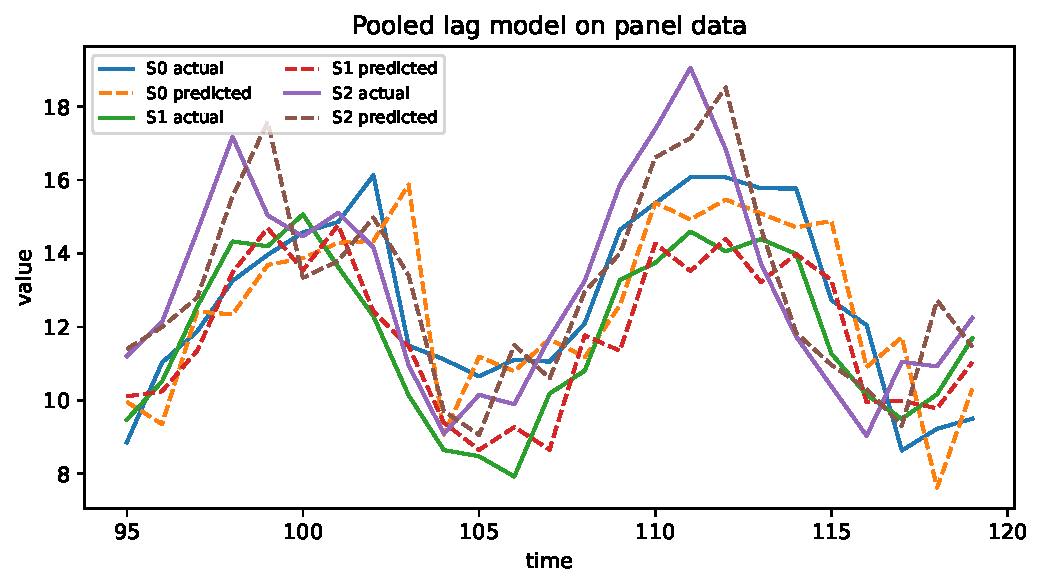
\includegraphics[keepaspectratio]{chapters/chapter-24-multivariate-panel-hierarchical_files/figure-pdf/ch24-python-panel-global-model-output-2.pdf}}

}

\caption{Actual and predicted values for several panel series using a
pooled lag model.}

\end{figure}%

\section{24.18 AI-assisted modeling
activity}\label{ai-assisted-modeling-activity-5}

\section{AI-assisted study box}\label{ai-assisted-study-box-3}

Ask an AI assistant to review a multivariate or hierarchical forecasting
workflow. Require the response to include:

\begin{enumerate}
\def\labelenumi{\arabic{enumi}.}
\tightlist
\item
  the assumed information set available at forecast time;
\item
  whether the model is local, multivariate, global, or hierarchical;
\item
  the aggregation matrix \(S\), if the problem is hierarchical;
\item
  a time-aware validation design;
\item
  at least two leakage risks;
\item
  one baseline model that should be hard to beat;
\item
  one diagnostic plot or statistical test;
\item
  a concise statement of what would make the model fail.
\end{enumerate}

Then verify each item manually. In particular, check whether every
feature used by the model would actually be known when the forecast is
made.

A useful prompt is:

\begin{quote}
I have multiple related time series with possible aggregation
constraints. Help me identify whether this is a multivariate, panel, or
hierarchical forecasting problem. State the mathematical model, the
validation split, the aggregation constraints, possible leakage risks,
and a simple baseline. Do not recommend a complex model until the
baseline and reconciliation constraints are clear.
\end{quote}

\section{24.19 Common mistakes}\label{common-mistakes-23}

\begin{enumerate}
\def\labelenumi{\arabic{enumi}.}
\tightlist
\item
  \textbf{Random train-test splitting.} Random splits leak future
  information into the training set.
\item
  \textbf{Ignoring aggregation constraints.} Independent forecasts for
  totals and parts are usually incoherent.
\item
  \textbf{Using unknown future covariates.} External regressors must be
  known, forecasted, or scenario-defined.
\item
  \textbf{Over-interpreting Granger prediction.} Predictive improvement
  is not structural causality.
\item
  \textbf{Fitting too many parameters.} VAR models become
  high-dimensional quickly: a VAR(\(p\)) with \(p_y\) variables has
  \(p\,p_y^2\) lag coefficients plus intercepts.
\item
  \textbf{Pooling unrelated series.} Global models help when series
  share structure, but can hurt when they do not.
\item
  \textbf{Reconciling after nonlinear transformations incorrectly.} If
  models are fit on log scale, aggregation on the original scale
  requires care.
\item
  \textbf{Forgetting contemporaneous correlation.} Multivariate forecast
  errors can be correlated even when point forecasts look reasonable.
\end{enumerate}

\section{24.20 Exercises}\label{exercises-23}

\begin{enumerate}
\def\labelenumi{\arabic{enumi}.}
\item
  Let \(\mathbf y_t=(y_{1t},y_{2t})^T\) follow a VAR(1) with \[
  A=\begin{bmatrix}0.6&0.3\\0&0.4\end{bmatrix}.
  \] Determine whether the process is stable. Compute the response after
  \(h=1,2,3\) steps to a unit shock in the second variable.
\item
  For the hierarchy \[
  \text{Total}=A+B+C+D,
  \] write the aggregation matrix \(S\) for \[
  \mathbf y_t=(\text{Total}_t,A_t,B_t,C_t,D_t)^T.
  \]
\item
  Suppose the base forecast is \[
  \widehat{\mathbf y}=(100,30,25,20,15)^T.
  \] Is it coherent? If not, compute the bottom-up reconciled forecast.
\item
  Explain why using next month's realized marketing spend as a feature
  for next month's demand forecast can be leakage unless that spend is
  known at forecast time.
\item
  Simulate a two-dimensional VAR(1) with one stable and one unstable
  coefficient matrix. Compare the sample paths.
\item
  Build a pooled lag model for a panel of at least five synthetic
  series. Compare it with separate local AR models.
\item
  Write a short explanation of the difference between cross-correlation,
  Granger prediction, and structural causality.
\item
  Implement OLS reconciliation for a two-level hierarchy and verify
  numerically that the reconciled forecasts are coherent.
\end{enumerate}

\section{24.21 Mini project}\label{mini-project-7}

Choose a dataset with multiple related time series. Examples include
product-by-store demand, regional energy usage, multiple financial
returns, enrollment by program, or sensor channels. Your report should
include:

\begin{enumerate}
\def\labelenumi{\arabic{enumi}.}
\tightlist
\item
  a description of the series structure: multivariate, panel,
  hierarchical, or a combination;
\item
  time plots and cross-correlation or lag-feature diagnostics;
\item
  at least one simple baseline;
\item
  one multivariate, global, or hierarchical model;
\item
  a time-aware validation design;
\item
  a check for forecast coherence if aggregation constraints exist;
\item
  an explanation of leakage risks;
\item
  a short AI-assisted critique and your verification of it.
\end{enumerate}

\section{24.22 Checklist}\label{checklist-8}

Before moving on, make sure you can answer the following questions.

\begin{itemize}
\tightlist
\item
  What is the difference between a multivariate time series and a panel
  of time series?
\item
  What does the matrix \(\Gamma(h)\) measure?
\item
  How do eigenvalues determine stability for a VAR(1)?
\item
  How is a VAR estimated by least squares?
\item
  What does an impulse response measure?
\item
  Why is Granger prediction not the same as causal proof?
\item
  What is an aggregation matrix \(S\)?
\item
  What does it mean for hierarchical forecasts to be coherent?
\item
  How does projection-based reconciliation work?
\item
  What leakage risks are common in panel and hierarchical forecasting?
\end{itemize}

\part{Part VII. Responsible AI, Projects, and Deployment}

\chapter{AI-Assisted Time-Series
Modeling}\label{ai-assisted-time-series-modeling}

\textbf{Part VII. Responsible AI, Projects, and Deployment}\\
\textbf{Chapter goal:} learn how to use AI assistants as modeling
partners without giving up mathematical control. We build AI-assisted
workflows for time-series forecasting, diagnose common failure modes
such as leakage and nonstationarity, write stronger prompts, verify code
and assumptions, and document responsible modeling decisions.

\section{Learning objectives}\label{learning-objectives-24}

After studying this chapter, you should be able to:

\begin{enumerate}
\def\labelenumi{\arabic{enumi}.}
\tightlist
\item
  explain where AI assistants can help in a time-series workflow and
  where they are risky;
\item
  distinguish \textbf{AI-generated suggestions} from
  \textbf{statistically verified conclusions};
\item
  design prompts that include task, data structure, time index, horizon,
  validation scheme, baselines, and diagnostics;
\item
  identify leakage in scaling, feature construction, random train/test
  splitting, target transformations, and future covariates;
\item
  use residual diagnostics and backtesting results to verify or reject
  an AI-suggested model;
\item
  write an AI-assisted modeling log that records assumptions, candidate
  models, evidence, and decisions;
\item
  use AI tools for code generation while checking correctness with small
  tests and baseline comparisons;
\item
  design a responsible final report that separates mathematical claims,
  empirical evidence, and speculation.
\end{enumerate}

\section{25.1 Why AI assistance changes the
workflow}\label{why-ai-assistance-changes-the-workflow}

A time-series modeling project has many decisions:

\[
\text{data} \rightarrow \text{cleaning} \rightarrow \text{features} \rightarrow \text{model} \rightarrow \text{validation} \rightarrow \text{forecast} \rightarrow \text{decision}.
\]

An AI assistant can help with each step. It can suggest transformations,
write Python code, explain residual plots, compare ARIMA with
machine-learning baselines, or draft a project report. But time series
create special risks. A model that looks good under a random split may
fail in production. A feature may accidentally use future information. A
transformation may be fitted using the entire sample. A model may
forecast a trend by extrapolating artifacts rather than learning a
stable pattern.

The goal of this chapter is not to treat AI as an oracle. The goal is to
use AI as a \textbf{modeling assistant} whose work must be checked by
mathematical reasoning and empirical validation.

\begin{tcolorbox}[enhanced jigsaw, arc=.35mm, bottomrule=.15mm, bottomtitle=1mm, breakable, colback=white, colbacktitle=quarto-callout-note-color!10!white, colframe=quarto-callout-note-color-frame, coltitle=black, left=2mm, leftrule=.75mm, opacityback=0, opacitybacktitle=0.6, rightrule=.15mm, title=\textcolor{quarto-callout-note-color}{\faInfo}\hspace{0.5em}{Main principle}, titlerule=0mm, toprule=.15mm, toptitle=1mm]

AI can propose. The analyst must verify.

A good AI-assisted workflow turns vague suggestions into testable
claims:

\[
\text{claim} \quad \longrightarrow \quad \text{diagnostic test} \quad \longrightarrow \quad \text{evidence} \quad \longrightarrow \quad \text{decision}.
\]

\end{tcolorbox}

\section{25.2 The mathematical object has not
changed}\label{the-mathematical-object-has-not-changed}

Let \(\{Y_t\}\) be the target process and let \(\mathcal F_t\) denote
the information available at time \(t\). A valid \(h\)-step-ahead
forecast must be a function of information available at the forecast
origin:

\[
\widehat Y_{t+h|t}=g_h(\mathcal F_t).
\]

The most important constraint is measurability:

\[
\widehat Y_{t+h|t}\ \text{must be }\mathcal F_t\text{-measurable}.
\]

This simply means that the forecast cannot depend on future observations
such as \(Y_{t+1},\ldots,Y_{t+h}\) or future covariates that would not
be known at time \(t\).

For example, the following feature is valid for one-step-ahead
prediction:

\[
X_{t,1}=Y_{t-1}.
\]

The following feature is invalid for forecasting \(Y_t\):

\[
X_{t,2}=\frac{Y_{t-1}+Y_t+Y_{t+1}}{3},
\]

because it uses the target value \(Y_t\) and a future value \(Y_{t+1}\).

\begin{tcolorbox}[enhanced jigsaw, arc=.35mm, bottomrule=.15mm, bottomtitle=1mm, breakable, colback=white, colbacktitle=quarto-callout-warning-color!10!white, colframe=quarto-callout-warning-color-frame, coltitle=black, left=2mm, leftrule=.75mm, opacityback=0, opacitybacktitle=0.6, rightrule=.15mm, title=\textcolor{quarto-callout-warning-color}{\faExclamationTriangle}\hspace{0.5em}{Leakage is a mathematical error}, titlerule=0mm, toprule=.15mm, toptitle=1mm]

Leakage is not merely a software bug. It violates the definition of
forecasting. A forecast made at time \(t\) must use only information
that would have been available at time \(t\).

\end{tcolorbox}

\section{25.3 AI as a modeling partner}\label{ai-as-a-modeling-partner}

AI assistance is useful when the task is structured. A strong workflow
separates four roles.

\textbf{1. Generator.} AI proposes candidate transformations, baselines,
models, diagnostics, and code.

\textbf{2. Explainer.} AI explains concepts such as differencing,
residual autocorrelation, horizon-wise error, or conformal prediction.

\textbf{3. Critic.} AI audits a workflow for leakage, weak baselines,
missing diagnostics, or overfitting.

\textbf{4. Editor.} AI helps turn mathematical and computational results
into a clear report.

The analyst should not ask, ``What is the best model?'' A better
question is:

\begin{quote}
Given the forecasting horizon, validation design, candidate models,
residual diagnostics, and baseline results below, identify possible
violations of time-series methodology and propose checks that can
confirm or reject each concern.
\end{quote}

This prompt asks for \textbf{auditable checks}, not unsupported
confidence.

\section{25.4 A formal AI-assisted modeling
loop}\label{a-formal-ai-assisted-modeling-loop}

A disciplined AI-assisted loop can be written as follows.

\begin{enumerate}
\def\labelenumi{\arabic{enumi}.}
\tightlist
\item
  Define the target and forecast origin.
\item
  Define \(\mathcal F_t\), the information available at prediction time.
\item
  Establish baselines.
\item
  Propose candidate models.
\item
  Use rolling-origin or chronological validation.
\item
  Diagnose residuals and calibration.
\item
  Ask AI to critique the workflow.
\item
  Verify each AI critique with code, plots, or mathematics.
\item
  Record the decision in a modeling log.
\end{enumerate}

Mathematically, suppose we compare \(M\) models over \(K\)
rolling-origin splits. Let \(e_{m,k,h}\) be the forecast error of model
\(m\) on split \(k\) and horizon \(h\):

\[
e_{m,k,h}=Y_{t_k+h}-\widehat Y^{(m)}_{t_k+h|t_k}.
\]

A horizon-wise mean squared error is

\[
\operatorname{MSE}_m(h)=\frac{1}{K}\sum_{k=1}^K e_{m,k,h}^2.
\]

The AI assistant may suggest model \(m^*\), but the decision should be
based on quantities such as \(\operatorname{MSE}_m(h)\), interval
coverage, residual diagnostics, interpretability, and operational
constraints.

\section{25.5 Prompt design for time-series
modeling}\label{prompt-design-for-time-series-modeling}

A time-series prompt should contain seven pieces of information.

{\def\LTcaptype{none} % do not increment counter
\begin{longtable}[]{@{}
  >{\raggedright\arraybackslash}p{(\linewidth - 2\tabcolsep) * \real{0.5000}}
  >{\raggedright\arraybackslash}p{(\linewidth - 2\tabcolsep) * \real{0.5000}}@{}}
\toprule\noalign{}
\begin{minipage}[b]{\linewidth}\raggedright
Component
\end{minipage} & \begin{minipage}[b]{\linewidth}\raggedright
What to include
\end{minipage} \\
\midrule\noalign{}
\endhead
\bottomrule\noalign{}
\endlastfoot
Target & What is being forecast or classified? \\
Time index & Frequency, irregularity, missing timestamps, calendar
structure \\
Forecast horizon & One-step, multi-step, fixed horizon, rolling
horizon \\
Available information & Which variables are known at forecast time? \\
Validation scheme & Chronological split, rolling-origin, blocked
cross-validation \\
Baselines & Naive, seasonal naive, mean, ARIMA, simple ML \\
Diagnostics & Residual ACF, Ljung-Box, calibration, horizon-wise
error \\
\end{longtable}
}

A useful template is:

\begin{tcolorbox}[enhanced jigsaw, arc=.35mm, bottomrule=.15mm, bottomtitle=1mm, breakable, colback=white, colbacktitle=quarto-callout-tip-color!10!white, colframe=quarto-callout-tip-color-frame, coltitle=black, left=2mm, leftrule=.75mm, opacityback=0, opacitybacktitle=0.6, rightrule=.15mm, title=\textcolor{quarto-callout-tip-color}{\faLightbulb}\hspace{0.5em}{AI prompt template}, titlerule=0mm, toprule=.15mm, toptitle=1mm]

I am modeling a time series with frequency {[}frequency{]}. The target
is {[}target{]}. The forecast horizon is {[}horizon{]}. At forecast
time, the available information is
\hyperref[information-set]{information set}. I used {[}validation
design{]} and compared against {[}baselines{]}. The candidate model is
{[}model{]}. Here are the residual diagnostics and error metrics:
{[}evidence{]}. Please identify possible methodological problems,
especially leakage, invalid validation, nonstationarity, missing
baselines, and unsupported claims. For each concern, give a concrete
verification step.

\end{tcolorbox}

\section{25.6 Interactive module: AI workflow
auditor}\label{interactive-module-ai-workflow-auditor}

This module turns common time-series modeling mistakes into a risk
score. It is not a replacement for reasoning. It is a teaching device
that helps students remember what to check before trusting a forecast.

Interactive Module: AI Forecasting Workflow Auditor

Select modeling choices. The module computes a risk score and gives an
audit summary. High risk means the workflow needs verification before
any forecast should be trusted.

Random train/test split was used instead of chronological or rolling
validation.

Scaling or imputation was fitted on the full dataset before splitting.

Some covariates may not be known at the forecast origin.

No naive or seasonal-naive baseline was reported.

Residual ACF, Ljung-Box, or calibration diagnostics were not checked.

Many models were tried, but only the best result was reported.

\protect\phantomsection\label{ch25_audit_plot}

\section{25.7 Interactive module: prompt
builder}\label{interactive-module-prompt-builder}

The next module builds a stronger prompt for asking an AI assistant to
critique a time-series project. The plot summarizes whether the prompt
contains the main pieces of forecasting context.

Interactive Module: Time-Series AI Prompt Builder

Choose the project context. The module builds a prompt that asks for
verification steps rather than unsupported model recommendations.

Task type: Forecasting Sequence classification Anomaly detection

Data frequency: Daily Weekly Monthly Irregular

Validation design: Rolling-origin backtesting Chronological holdout
Blocked cross-validation Random split

Model family: SARIMA Prophet-type additive model Gradient boosting with
lag features LSTM or GRU Transformer forecaster

Include residual diagnostics? Yes Partial No

Include baseline comparison? Yes No

\protect\phantomsection\label{ch25_prompt_plot}

\section{25.8 Common AI failure modes in time-series
work}\label{common-ai-failure-modes-in-time-series-work}

AI tools often make plausible but invalid suggestions. Common failures
include the following.

\textbf{Random splits for forecasting.} Random splits mix past and
future. They are usually invalid because future observations influence
model tuning and evaluation.

\textbf{Global preprocessing leakage.} If a scaler is fitted on the full
dataset, then future means and variances affect training.

\textbf{Target leakage through rolling features.} A centered rolling
average uses future observations. Forecasting features should be lagged
or one-sided.

\textbf{Ignoring the forecast horizon.} A model good for one-step
prediction may perform poorly for \(h=12\).

\textbf{Ignoring baselines.} A complex neural network that does not beat
seasonal naive is not useful.

\textbf{Misreading residuals.} Small training error does not imply
residual white noise.

\textbf{Confusing correlation with causation.} A lagged variable may
help prediction without being a causal driver.

\textbf{Over-trusting generated code.} AI-generated code may run but
silently use future data.

\begin{tcolorbox}[enhanced jigsaw, arc=.35mm, bottomrule=.15mm, bottomtitle=1mm, breakable, colback=white, colbacktitle=quarto-callout-important-color!10!white, colframe=quarto-callout-important-color-frame, coltitle=black, left=2mm, leftrule=.75mm, opacityback=0, opacitybacktitle=0.6, rightrule=.15mm, title=\textcolor{quarto-callout-important-color}{\faExclamation}\hspace{0.5em}{Verification rule}, titlerule=0mm, toprule=.15mm, toptitle=1mm]

Every AI-generated modeling claim should be converted into at least one
of the following:

\[
\text{plot},\quad \text{statistic},\quad \text{unit test},\quad \text{mathematical condition},\quad \text{backtest comparison}.
\]

\end{tcolorbox}

\section{25.9 Python example: random split versus chronological
split}\label{python-example-random-split-versus-chronological-split}

The next example shows why random splits can be misleading. We create
lag features for a trending seasonal series. Then we compare a random
split with a chronological split using the same linear model. The two
designs answer different questions. The random split allows training
observations to be distributed throughout the whole time range, while
the chronological split evaluates prediction on a future block. The
random-split error may look artificially strong, but the main problem is
more fundamental: it is not the operational forecasting task.

\begin{Shaded}
\begin{Highlighting}[]
\ImportTok{import}\NormalTok{ numpy }\ImportTok{as}\NormalTok{ np}
\ImportTok{import}\NormalTok{ matplotlib.pyplot }\ImportTok{as}\NormalTok{ plt}

\NormalTok{rng }\OperatorTok{=}\NormalTok{ np.random.default\_rng(}\DecValTok{7339}\NormalTok{)}
\NormalTok{n }\OperatorTok{=} \DecValTok{260}
\NormalTok{t }\OperatorTok{=}\NormalTok{ np.arange(n)}
\NormalTok{y }\OperatorTok{=} \FloatTok{0.03} \OperatorTok{*}\NormalTok{ t }\OperatorTok{+} \FloatTok{2.0} \OperatorTok{*}\NormalTok{ np.sin(}\DecValTok{2} \OperatorTok{*}\NormalTok{ np.pi }\OperatorTok{*}\NormalTok{ t }\OperatorTok{/} \DecValTok{24}\NormalTok{) }\OperatorTok{+}\NormalTok{ rng.normal(}\DecValTok{0}\NormalTok{, }\FloatTok{0.6}\NormalTok{, n)}

\CommentTok{\# Build lag features using only past values.}
\KeywordTok{def}\NormalTok{ make\_lag\_matrix(series, max\_lag):}
\NormalTok{    X, target, times }\OperatorTok{=}\NormalTok{ [], [], []}
    \ControlFlowTok{for}\NormalTok{ i }\KeywordTok{in} \BuiltInTok{range}\NormalTok{(max\_lag, }\BuiltInTok{len}\NormalTok{(series)):}
\NormalTok{        X.append([series[i }\OperatorTok{{-}}\NormalTok{ lag] }\ControlFlowTok{for}\NormalTok{ lag }\KeywordTok{in} \BuiltInTok{range}\NormalTok{(}\DecValTok{1}\NormalTok{, max\_lag }\OperatorTok{+} \DecValTok{1}\NormalTok{)])}
\NormalTok{        target.append(series[i])}
\NormalTok{        times.append(i)}
    \ControlFlowTok{return}\NormalTok{ np.asarray(X), np.asarray(target), np.asarray(times)}

\NormalTok{X, target, times }\OperatorTok{=}\NormalTok{ make\_lag\_matrix(y, max\_lag}\OperatorTok{=}\DecValTok{12}\NormalTok{)}
\NormalTok{X\_design }\OperatorTok{=}\NormalTok{ np.column\_stack([np.ones(}\BuiltInTok{len}\NormalTok{(X)), X])}

\CommentTok{\# Chronological split.}
\NormalTok{cut }\OperatorTok{=} \BuiltInTok{int}\NormalTok{(}\FloatTok{0.75} \OperatorTok{*} \BuiltInTok{len}\NormalTok{(X\_design))}
\NormalTok{X\_train\_c, X\_test\_c }\OperatorTok{=}\NormalTok{ X\_design[:cut], X\_design[cut:]}
\NormalTok{y\_train\_c, y\_test\_c }\OperatorTok{=}\NormalTok{ target[:cut], target[cut:]}
\NormalTok{time\_test\_c }\OperatorTok{=}\NormalTok{ times[cut:]}

\NormalTok{beta\_c }\OperatorTok{=}\NormalTok{ np.linalg.lstsq(X\_train\_c, y\_train\_c, rcond}\OperatorTok{=}\VariableTok{None}\NormalTok{)[}\DecValTok{0}\NormalTok{]}
\NormalTok{pred\_c }\OperatorTok{=}\NormalTok{ X\_test\_c }\OperatorTok{@}\NormalTok{ beta\_c}
\NormalTok{mse\_c }\OperatorTok{=}\NormalTok{ np.mean((y\_test\_c }\OperatorTok{{-}}\NormalTok{ pred\_c) }\OperatorTok{**} \DecValTok{2}\NormalTok{)}

\CommentTok{\# Random split: invalid for forecasting evaluation, but common in ordinary ML.}
\NormalTok{indices }\OperatorTok{=}\NormalTok{ np.arange(}\BuiltInTok{len}\NormalTok{(X\_design))}
\NormalTok{rng.shuffle(indices)}
\NormalTok{train\_size }\OperatorTok{=}\NormalTok{ cut}
\NormalTok{train\_idx }\OperatorTok{=}\NormalTok{ indices[:train\_size]}
\NormalTok{test\_idx }\OperatorTok{=}\NormalTok{ indices[train\_size:]}

\NormalTok{beta\_r }\OperatorTok{=}\NormalTok{ np.linalg.lstsq(X\_design[train\_idx], target[train\_idx], rcond}\OperatorTok{=}\VariableTok{None}\NormalTok{)[}\DecValTok{0}\NormalTok{]}
\NormalTok{pred\_r }\OperatorTok{=}\NormalTok{ X\_design[test\_idx] }\OperatorTok{@}\NormalTok{ beta\_r}
\NormalTok{mse\_r }\OperatorTok{=}\NormalTok{ np.mean((target[test\_idx] }\OperatorTok{{-}}\NormalTok{ pred\_r) }\OperatorTok{**} \DecValTok{2}\NormalTok{)}

\BuiltInTok{print}\NormalTok{(}\SpecialStringTok{f"Random{-}split MSE:        }\SpecialCharTok{\{}\NormalTok{mse\_r}\SpecialCharTok{:.3f\}}\SpecialStringTok{"}\NormalTok{)}
\BuiltInTok{print}\NormalTok{(}\SpecialStringTok{f"Chronological{-}split MSE: }\SpecialCharTok{\{}\NormalTok{mse\_c}\SpecialCharTok{:.3f\}}\SpecialStringTok{"}\NormalTok{)}

\NormalTok{plt.figure(figsize}\OperatorTok{=}\NormalTok{(}\DecValTok{8}\NormalTok{, }\DecValTok{4}\NormalTok{))}
\NormalTok{plt.plot(t, y, label}\OperatorTok{=}\StringTok{"observed"}\NormalTok{)}
\NormalTok{plt.axvline(times[cut], linestyle}\OperatorTok{=}\StringTok{"{-}{-}"}\NormalTok{, label}\OperatorTok{=}\StringTok{"chronological split"}\NormalTok{)}
\NormalTok{plt.plot(time\_test\_c, pred\_c, label}\OperatorTok{=}\StringTok{"chronological forecast"}\NormalTok{)}
\NormalTok{plt.xlabel(}\StringTok{"time"}\NormalTok{)}
\NormalTok{plt.ylabel(}\StringTok{"value"}\NormalTok{)}
\NormalTok{plt.title(}\StringTok{"Chronological evaluation: forecasting the future block"}\NormalTok{)}
\NormalTok{plt.legend()}
\NormalTok{plt.show()}
\end{Highlighting}
\end{Shaded}

\begin{verbatim}
Random-split MSE:        0.621
Chronological-split MSE: 0.519
\end{verbatim}

\begin{figure}[H]

{\centering \pandocbounded{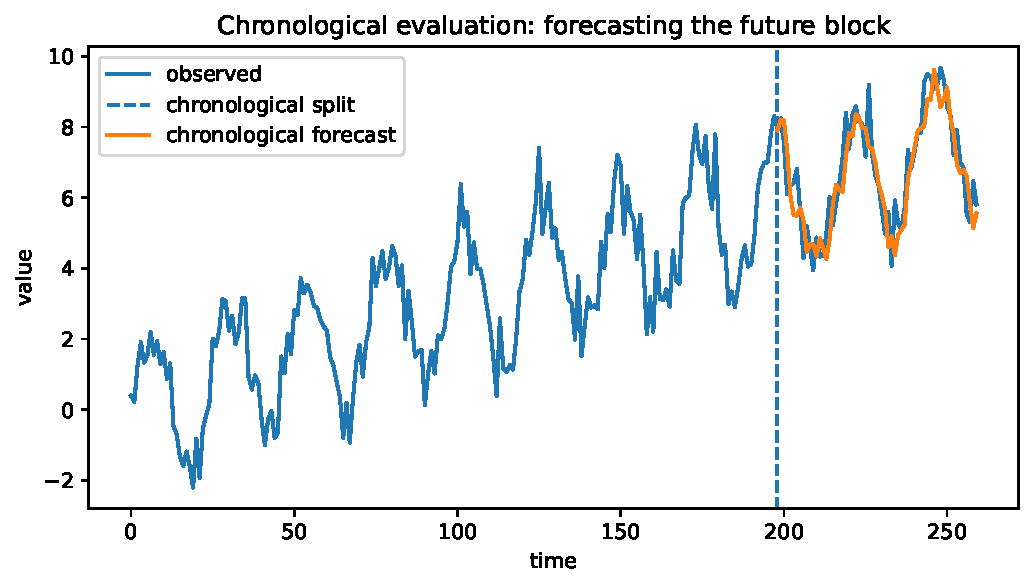
\includegraphics[keepaspectratio]{chapters/chapter-25-ai-assisted-time-series-modeling_files/figure-pdf/ch25-python-random-vs-chronological-output-2.pdf}}

}

\caption{Random split and chronological split evaluate different
forecasting tasks.}

\end{figure}%

The random split is not estimating the same operational task. Its error
can be smaller or larger in a simulation, but it does not answer the
forecasting question. In forecasting, the relevant question is usually:
given the past, can we predict the future?

\section{25.10 Python example: an audit checklist as
code}\label{python-example-an-audit-checklist-as-code}

A modeling checklist can be written as a function. This makes the audit
reproducible and encourages students to translate vague concerns into
explicit checks.

\protect\phantomsection\label{ch25-python-audit-checklist}
\begin{Shaded}
\begin{Highlighting}[]
\ImportTok{from}\NormalTok{ dataclasses }\ImportTok{import}\NormalTok{ dataclass}

\AttributeTok{@dataclass}
\KeywordTok{class}\NormalTok{ ForecastWorkflow:}
\NormalTok{    validation: }\BuiltInTok{str}
\NormalTok{    scaler\_fit: }\BuiltInTok{str}
\NormalTok{    has\_baseline: }\BuiltInTok{bool}
\NormalTok{    residual\_diagnostics: }\BuiltInTok{bool}
\NormalTok{    future\_covariates\_known: }\BuiltInTok{bool}
\NormalTok{    reported\_all\_model\_trials: }\BuiltInTok{bool}


\KeywordTok{def}\NormalTok{ audit\_workflow(workflow):}
\NormalTok{    issues }\OperatorTok{=}\NormalTok{ []}

    \ControlFlowTok{if}\NormalTok{ workflow.validation.lower() }\KeywordTok{in}\NormalTok{ \{}\StringTok{"random"}\NormalTok{, }\StringTok{"random split"}\NormalTok{, }\StringTok{"shuffle"}\NormalTok{\}:}
\NormalTok{        issues.append(}\StringTok{"Use chronological or rolling{-}origin validation instead of a random split."}\NormalTok{)}

    \ControlFlowTok{if}\NormalTok{ workflow.scaler\_fit.lower() }\OperatorTok{==} \StringTok{"full data"}\NormalTok{:}
\NormalTok{        issues.append(}\StringTok{"Fit scalers/imputers on each training fold only, not on the full dataset."}\NormalTok{)}

    \ControlFlowTok{if} \KeywordTok{not}\NormalTok{ workflow.has\_baseline:}
\NormalTok{        issues.append(}\StringTok{"Add naive and seasonal{-}naive baselines before claiming improvement."}\NormalTok{)}

    \ControlFlowTok{if} \KeywordTok{not}\NormalTok{ workflow.residual\_diagnostics:}
\NormalTok{        issues.append(}\StringTok{"Check residual ACF, Ljung{-}Box statistic, and horizon{-}wise errors."}\NormalTok{)}

    \ControlFlowTok{if} \KeywordTok{not}\NormalTok{ workflow.future\_covariates\_known:}
\NormalTok{        issues.append(}\StringTok{"Remove or replace covariates that are unavailable at the forecast origin."}\NormalTok{)}

    \ControlFlowTok{if} \KeywordTok{not}\NormalTok{ workflow.reported\_all\_model\_trials:}
\NormalTok{        issues.append(}\StringTok{"Report the tuning protocol to reduce selection bias."}\NormalTok{)}

    \ControlFlowTok{if} \KeywordTok{not}\NormalTok{ issues:}
\NormalTok{        issues.append(}\StringTok{"No major issue detected, but still inspect plots and backtests."}\NormalTok{)}

    \ControlFlowTok{return}\NormalTok{ issues}

\NormalTok{example }\OperatorTok{=}\NormalTok{ ForecastWorkflow(}
\NormalTok{    validation}\OperatorTok{=}\StringTok{"random split"}\NormalTok{,}
\NormalTok{    scaler\_fit}\OperatorTok{=}\StringTok{"full data"}\NormalTok{,}
\NormalTok{    has\_baseline}\OperatorTok{=}\VariableTok{False}\NormalTok{,}
\NormalTok{    residual\_diagnostics}\OperatorTok{=}\VariableTok{True}\NormalTok{,}
\NormalTok{    future\_covariates\_known}\OperatorTok{=}\VariableTok{False}\NormalTok{,}
\NormalTok{    reported\_all\_model\_trials}\OperatorTok{=}\VariableTok{False}\NormalTok{,}
\NormalTok{)}

\ControlFlowTok{for}\NormalTok{ k, issue }\KeywordTok{in} \BuiltInTok{enumerate}\NormalTok{(audit\_workflow(example), start}\OperatorTok{=}\DecValTok{1}\NormalTok{):}
    \BuiltInTok{print}\NormalTok{(}\SpecialStringTok{f"}\SpecialCharTok{\{}\NormalTok{k}\SpecialCharTok{\}}\SpecialStringTok{. }\SpecialCharTok{\{}\NormalTok{issue}\SpecialCharTok{\}}\SpecialStringTok{"}\NormalTok{)}
\end{Highlighting}
\end{Shaded}

\begin{verbatim}
1. Use chronological or rolling-origin validation instead of a random split.
2. Fit scalers/imputers on each training fold only, not on the full dataset.
3. Add naive and seasonal-naive baselines before claiming improvement.
4. Remove or replace covariates that are unavailable at the forecast origin.
5. Report the tuning protocol to reduce selection bias.
\end{verbatim}

\section{25.11 Python example: residual diagnostics after an
AI-suggested
model}\label{python-example-residual-diagnostics-after-an-ai-suggested-model}

Suppose an AI assistant suggests a lag-1 autoregression. We should check
whether the residuals still contain autocorrelation. The next code fits
a simple AR(1)-style regression to data that actually has seasonality.
The residual ACF reveals remaining structure.

\begin{Shaded}
\begin{Highlighting}[]
\ImportTok{import}\NormalTok{ numpy }\ImportTok{as}\NormalTok{ np}
\ImportTok{import}\NormalTok{ matplotlib.pyplot }\ImportTok{as}\NormalTok{ plt}

\NormalTok{rng }\OperatorTok{=}\NormalTok{ np.random.default\_rng(}\DecValTok{2025}\NormalTok{)}
\NormalTok{n }\OperatorTok{=} \DecValTok{220}
\NormalTok{t }\OperatorTok{=}\NormalTok{ np.arange(n)}
\NormalTok{y }\OperatorTok{=} \FloatTok{0.7} \OperatorTok{*}\NormalTok{ np.sin(}\DecValTok{2} \OperatorTok{*}\NormalTok{ np.pi }\OperatorTok{*}\NormalTok{ t }\OperatorTok{/} \DecValTok{12}\NormalTok{) }\OperatorTok{+} \FloatTok{0.6} \OperatorTok{*}\NormalTok{ np.sin(}\DecValTok{2} \OperatorTok{*}\NormalTok{ np.pi }\OperatorTok{*}\NormalTok{ t }\OperatorTok{/} \DecValTok{36}\NormalTok{) }\OperatorTok{+}\NormalTok{ rng.normal(}\DecValTok{0}\NormalTok{, }\FloatTok{0.4}\NormalTok{, n)}

\CommentTok{\# AI{-}suggested simple model: y\_t = a + phi y\_\{t{-}1\} + error.}
\NormalTok{X }\OperatorTok{=}\NormalTok{ np.column\_stack([np.ones(n }\OperatorTok{{-}} \DecValTok{1}\NormalTok{), y[:}\OperatorTok{{-}}\DecValTok{1}\NormalTok{]])}
\NormalTok{y\_response }\OperatorTok{=}\NormalTok{ y[}\DecValTok{1}\NormalTok{:]}
\NormalTok{beta }\OperatorTok{=}\NormalTok{ np.linalg.lstsq(X, y\_response, rcond}\OperatorTok{=}\VariableTok{None}\NormalTok{)[}\DecValTok{0}\NormalTok{]}
\NormalTok{fitted }\OperatorTok{=}\NormalTok{ X }\OperatorTok{@}\NormalTok{ beta}
\NormalTok{resid }\OperatorTok{=}\NormalTok{ y\_response }\OperatorTok{{-}}\NormalTok{ fitted}


\KeywordTok{def}\NormalTok{ sample\_acf(x, max\_lag):}
\NormalTok{    x }\OperatorTok{=}\NormalTok{ np.asarray(x)}
\NormalTok{    x }\OperatorTok{=}\NormalTok{ x }\OperatorTok{{-}}\NormalTok{ x.mean()}
\NormalTok{    denom }\OperatorTok{=}\NormalTok{ np.}\BuiltInTok{sum}\NormalTok{(x }\OperatorTok{**} \DecValTok{2}\NormalTok{)}
\NormalTok{    values }\OperatorTok{=}\NormalTok{ []}
    \ControlFlowTok{for}\NormalTok{ h }\KeywordTok{in} \BuiltInTok{range}\NormalTok{(max\_lag }\OperatorTok{+} \DecValTok{1}\NormalTok{):}
\NormalTok{        values.append(np.}\BuiltInTok{sum}\NormalTok{(x[h:] }\OperatorTok{*}\NormalTok{ x[:}\BuiltInTok{len}\NormalTok{(x) }\OperatorTok{{-}}\NormalTok{ h]) }\OperatorTok{/}\NormalTok{ denom)}
    \ControlFlowTok{return}\NormalTok{ np.asarray(values)}

\NormalTok{r }\OperatorTok{=}\NormalTok{ sample\_acf(resid, }\DecValTok{30}\NormalTok{)}
\NormalTok{conf }\OperatorTok{=} \FloatTok{1.96} \OperatorTok{/}\NormalTok{ np.sqrt(}\BuiltInTok{len}\NormalTok{(resid))}

\NormalTok{plt.figure(figsize}\OperatorTok{=}\NormalTok{(}\DecValTok{8}\NormalTok{, }\DecValTok{4}\NormalTok{))}
\NormalTok{plt.stem(np.arange(}\BuiltInTok{len}\NormalTok{(r)), r)}
\NormalTok{plt.axhline(conf, linestyle}\OperatorTok{=}\StringTok{"{-}{-}"}\NormalTok{)}
\NormalTok{plt.axhline(}\OperatorTok{{-}}\NormalTok{conf, linestyle}\OperatorTok{=}\StringTok{"{-}{-}"}\NormalTok{)}
\NormalTok{plt.xlabel(}\StringTok{"lag"}\NormalTok{)}
\NormalTok{plt.ylabel(}\StringTok{"residual ACF"}\NormalTok{)}
\NormalTok{plt.title(}\StringTok{"Residual ACF after a simple AI{-}suggested AR(1) model"}\NormalTok{)}
\NormalTok{plt.show()}

\BuiltInTok{print}\NormalTok{(}\SpecialStringTok{f"Estimated intercept: }\SpecialCharTok{\{}\NormalTok{beta[}\DecValTok{0}\NormalTok{]}\SpecialCharTok{:.3f\}}\SpecialStringTok{"}\NormalTok{)}
\BuiltInTok{print}\NormalTok{(}\SpecialStringTok{f"Estimated phi:       }\SpecialCharTok{\{}\NormalTok{beta[}\DecValTok{1}\NormalTok{]}\SpecialCharTok{:.3f\}}\SpecialStringTok{"}\NormalTok{)}
\BuiltInTok{print}\NormalTok{(}\SpecialStringTok{f"Approximate ACF significance band: +/{-} }\SpecialCharTok{\{}\NormalTok{conf}\SpecialCharTok{:.3f\}}\SpecialStringTok{"}\NormalTok{)}
\end{Highlighting}
\end{Shaded}

\begin{figure}[H]

{\centering \pandocbounded{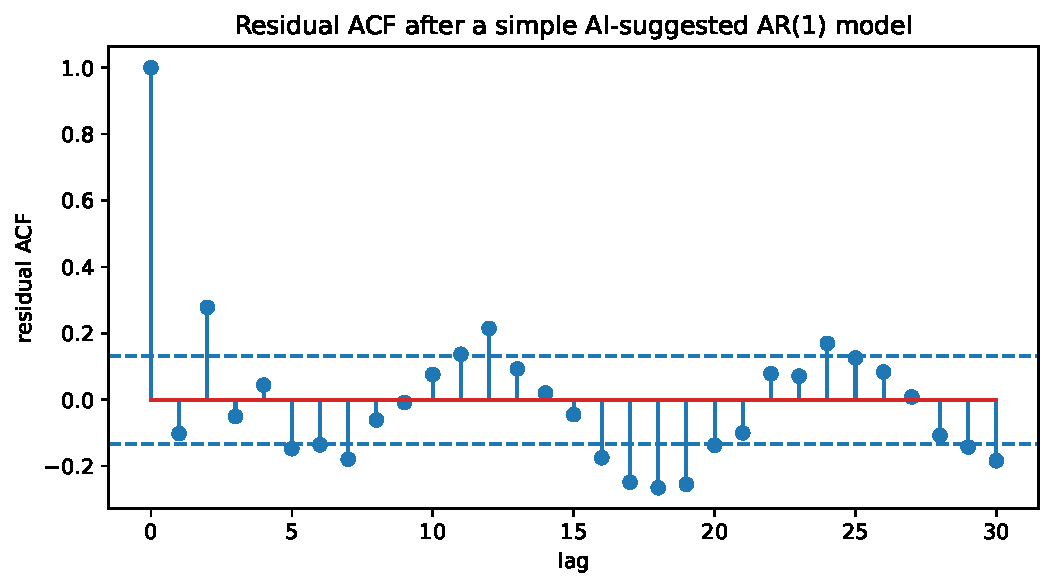
\includegraphics[keepaspectratio]{chapters/chapter-25-ai-assisted-time-series-modeling_files/figure-pdf/ch25-python-residual-acf-output-1.pdf}}

}

\caption{Residual autocorrelation can reveal structure missed by a
suggested model.}

\end{figure}%

\begin{verbatim}
Estimated intercept: 0.003
Estimated phi:       0.662
Approximate ACF significance band: +/- 0.132
\end{verbatim}

If residual autocorrelations remain significant, the proposed model has
not captured all predictable structure. The next step might be a
seasonal model, Fourier features, SARIMA, or a nonlinear model,
depending on the validation results.

\section{25.12 AI-assisted model
criticism}\label{ai-assisted-model-criticism-1}

A useful AI critic prompt should be specific and adversarial. For
example:

\begin{tcolorbox}[enhanced jigsaw, arc=.35mm, bottomrule=.15mm, bottomtitle=1mm, breakable, colback=white, colbacktitle=quarto-callout-tip-color!10!white, colframe=quarto-callout-tip-color-frame, coltitle=black, left=2mm, leftrule=.75mm, opacityback=0, opacitybacktitle=0.6, rightrule=.15mm, title=\textcolor{quarto-callout-tip-color}{\faLightbulb}\hspace{0.5em}{Strong critic prompt}, titlerule=0mm, toprule=.15mm, toptitle=1mm]

Here is my time-series forecasting workflow. Please act as a skeptical
reviewer. Identify any possible leakage, invalid validation, weak
baseline comparison, inappropriate transformation, or unsupported
conclusion. For each issue, give a concrete test I can run. Do not
recommend a more complex model unless the evidence shows that the
current residuals contain predictable structure.

\end{tcolorbox}

The phrase ``do not recommend a more complex model unless\ldots'' is
important. It pushes the assistant away from automatic complexity and
toward evidence-based modeling.

\section{25.13 AI-assisted code review}\label{ai-assisted-code-review}

When AI writes code, students should check at least five properties.

\begin{enumerate}
\def\labelenumi{\arabic{enumi}.}
\tightlist
\item
  \textbf{Time ordering.} Does the split preserve time order?
\item
  \textbf{Feature timing.} Is every feature known at the forecast
  origin?
\item
  \textbf{Preprocessing scope.} Are scalers and imputers fitted only on
  training data?
\item
  \textbf{Target alignment.} Are inputs and labels shifted correctly?
\item
  \textbf{Evaluation horizon.} Does the error metric match the intended
  horizon?
\end{enumerate}

A small unit test can be more valuable than reading a long generated
script. For example, if a window has input length \(L\) and horizon
\(H\), then the label for window starting at \(s\) should begin at time
\(s+L\):

\[
\text{input}=(Y_s,\ldots,Y_{s+L-1}),
\qquad
\text{label}=(Y_{s+L},\ldots,Y_{s+L+H-1}).
\]

If code instead uses \(Y_{s+L-1}\) as part of the label, the model may
be trained to reproduce a value that is also in the input.

\section{25.14 AI-assisted reporting}\label{ai-assisted-reporting}

A strong report separates four kinds of statements.

\textbf{Mathematical assumptions.} Example: ``The SARIMA model assumes
the seasonally differenced process is stationary.''

\textbf{Empirical evidence.} Example: ``In rolling-origin validation,
SARIMA had lower MASE than seasonal naive for horizons 1--6.''

\textbf{Diagnostic evidence.} Example: ``Residual ACF did not show
significant autocorrelation beyond lag 2.''

\textbf{Limitations.} Example: ``The validation period contains only one
holiday season, so holiday effects are uncertain.''

AI can help write the report, but the evidence must come from the
analysis.

\section{25.15 AI component: prompts for
students}\label{ai-component-prompts-for-students}

Use the following prompts during homework or projects.

\subsection{Prompt A: model diagnosis}\label{prompt-a-model-diagnosis}

\begin{quote}
I fitted {[}model{]} to \hyperref[data-description]{data description}
using {[}validation scheme{]}. Here are horizon-wise errors, residual
ACF, and baseline comparisons. Identify what assumptions may be
violated. For each issue, tell me what plot, statistic, or backtest
would verify it.
\end{quote}

\subsection{Prompt B: leakage audit}\label{prompt-b-leakage-audit}

\begin{quote}
Review this feature-construction code for time leakage. The forecast
horizon is {[}horizon{]}. At the forecast origin, the available
variables are {[}list{]}. Identify every line that may use future
information.
\end{quote}

\subsection{Prompt C: report
improvement}\label{prompt-c-report-improvement}

\begin{quote}
Rewrite this model-comparison paragraph so that it clearly distinguishes
assumptions, evidence, and limitations. Do not claim causality. Do not
claim superiority unless supported by the validation results.
\end{quote}

\subsection{Prompt D: mathematical
explanation}\label{prompt-d-mathematical-explanation}

\begin{quote}
Explain why a random train/test split is invalid for this forecasting
problem using the information-set notation \(\mathcal F_t\).
\end{quote}

\section{25.16 Common mistakes}\label{common-mistakes-24}

\begin{enumerate}
\def\labelenumi{\arabic{enumi}.}
\tightlist
\item
  Asking AI for ``the best model'' before defining the horizon and
  validation scheme.
\item
  Reporting only the model that won after many experiments.
\item
  Using random cross-validation on temporally dependent observations.
\item
  Letting future values enter rolling features, scalers, or imputers.
\item
  Comparing a complex model only against weak baselines.
\item
  Accepting AI-generated code because it runs.
\item
  Ignoring residual ACF after fitting a model.
\item
  Treating AI explanations as citations or empirical evidence.
\item
  Asking AI to interpret a plot without showing the data-generating
  context.
\item
  Writing a report that hides uncertainty, failed models, or
  limitations.
\end{enumerate}

\section{25.17 Mini project: AI-assisted audit of a forecasting
pipeline}\label{mini-project-ai-assisted-audit-of-a-forecasting-pipeline}

Choose a time-series dataset and complete the following.

\begin{enumerate}
\def\labelenumi{\arabic{enumi}.}
\tightlist
\item
  Define the forecast target, horizon, and information set
  \(\mathcal F_t\).
\item
  Build at least two baselines.
\item
  Build one classical model and one machine-learning or deep-learning
  model.
\item
  Evaluate all models using chronological or rolling-origin validation.
\item
  Ask an AI assistant to audit the workflow for leakage and unsupported
  claims.
\item
  Verify or reject each AI concern using code, plots, or mathematical
  reasoning.
\item
  Submit a modeling log that records prompts, AI suggestions,
  verification steps, and final decisions.
\end{enumerate}

The final report should include a section titled \textbf{AI Assistance
and Verification}.

\section{25.18 Exercises}\label{exercises-24}

\begin{enumerate}
\def\labelenumi{\arabic{enumi}.}
\item
  Let \(\mathcal F_t=\sigma(Y_1,\ldots,Y_t)\). Explain why a centered
  rolling mean \(m_t=(Y_{t-1}+Y_t+Y_{t+1})/3\) is invalid as a feature
  for forecasting \(Y_t\).
\item
  Suppose an AI assistant recommends random five-fold cross-validation
  for a monthly forecasting problem. Write a response explaining why
  this is usually invalid and propose an alternative validation design.
\item
  Construct a valid supervised-learning matrix for forecasting
  \(Y_{t+3}\) using lags \(Y_t,Y_{t-1},\ldots,Y_{t-11}\). State the
  input row and label for a forecast origin \(t\).
\item
  An AI-generated model beats ARIMA but not seasonal naive. What
  conclusion should the analyst draw?
\item
  Write a prompt that asks an AI assistant to diagnose residual
  autocorrelation without recommending a more complex model unless the
  evidence supports it.
\item
  A scaler is fitted on the full dataset before a chronological split.
  Explain the leakage and rewrite the workflow correctly.
\item
  Let \(e_{k,h}\) be forecast errors over rolling-origin splits. Define
  horizon-wise RMSE and explain why averaging over all horizons may hide
  poor long-horizon performance.
\item
  Design a unit test for a windowing function with input length \(L=24\)
  and forecast horizon \(H=12\).
\item
  Give one example where AI can help with a time-series project and one
  example where AI can mislead the analyst.
\item
  Write a short model-card paragraph for a forecasting model that
  includes target, horizon, validation scheme, baselines, diagnostics,
  and limitations.
\end{enumerate}

\section{25.19 Chapter checklist}\label{chapter-checklist-15}

You should now be able to:

\begin{itemize}
\tightlist
\item[$\square$]
  define the forecast information set \(\mathcal F_t\);
\item[$\square$]
  explain why leakage violates the forecasting problem;
\item[$\square$]
  write prompts that include target, horizon, validation, baselines, and
  diagnostics;
\item[$\square$]
  use AI as generator, explainer, critic, and editor;
\item[$\square$]
  verify AI-generated claims with plots, statistics, unit tests, or
  backtests;
\item[$\square$]
  audit feature construction for future information;
\item[$\square$]
  distinguish model evidence from AI-generated explanation;
\item[$\square$]
  write a responsible AI-assisted modeling log.
\end{itemize}

\section{25.20 Further reading}\label{further-reading-5}

\begin{itemize}
\tightlist
\item
  Shumway and Stoffer, \emph{Time Series Analysis and Its Applications},
  for classical modeling and diagnostics.
\item
  Hyndman and Athanasopoulos, \emph{Forecasting: Principles and
  Practice}, for validation, baselines, and practical forecasting
  workflows.
\item
  Goodfellow, Bengio, and Courville, \emph{Deep Learning}, for
  neural-network modeling principles.
\item
  Recent documentation of the software packages used in your project,
  because package APIs and defaults change over time.
\end{itemize}

\chapter{End-to-End Forecasting
Pipeline}\label{end-to-end-forecasting-pipeline}

\textbf{Part VII. Responsible AI, Projects, and Deployment}\\
\textbf{Chapter goal:} build a complete, reproducible forecasting
workflow from raw ordered data to a forecast report. We connect
mathematical information sets, preprocessing, feature construction,
baseline modeling, validation, uncertainty, monitoring, and AI-assisted
quality control.

\section{Learning objectives}\label{learning-objectives-25}

After studying this chapter, you should be able to:

\begin{enumerate}
\def\labelenumi{\arabic{enumi}.}
\tightlist
\item
  define the forecasting target, forecast origin, horizon, and
  information set for an applied problem;
\item
  design a leakage-safe preprocessing and feature-engineering pipeline;
\item
  construct baseline, statistical, and machine-learning forecasting
  models in a reproducible workflow;
\item
  use chronological validation and rolling-origin evaluation to compare
  candidate models;
\item
  evaluate point forecasts, intervals, and residual behavior;
\item
  package forecasts into a report that records assumptions, diagnostics,
  and model limitations;
\item
  identify the difference between validation performance and deployment
  performance;
\item
  use AI assistance as a workflow critic while verifying every
  suggestion with code, mathematics, or diagnostics.
\end{enumerate}

\section{26.1 Why an end-to-end pipeline
matters}\label{why-an-end-to-end-pipeline-matters}

A forecasting model is only one part of a forecasting system. In
practice, students and analysts often spend most of their time on the
surrounding decisions:

\[
\text{raw data}
\rightarrow
\text{cleaning}
\rightarrow
\text{target definition}
\rightarrow
\text{features}
\rightarrow
\text{model fitting}
\rightarrow
\text{validation}
\rightarrow
\text{forecast report}
\rightarrow
\text{monitoring}.
\]

A mathematically strong model can fail if any step is invalid. A random
train--test split can make a weak model look excellent. A rolling mean
can accidentally use the target value being predicted. A model can beat
ARIMA on one validation split but fail under a different forecast
horizon. An interval forecast can look impressive but miss the true
value too often.

The purpose of this chapter is to make the whole workflow explicit. We
treat forecasting as an operation performed at a \textbf{forecast
origin}. At time \(t\), the analyst has an information set
\(\mathcal F_t\). A valid \(h\)-step-ahead forecast must satisfy

\[
\widehat Y_{t+h|t}=g_h(\mathcal F_t).
\]

This condition is the organizing principle for the entire pipeline.

\begin{tcolorbox}[enhanced jigsaw, arc=.35mm, bottomrule=.15mm, bottomtitle=1mm, breakable, colback=white, colbacktitle=quarto-callout-warning-color!10!white, colframe=quarto-callout-warning-color-frame, coltitle=black, left=2mm, leftrule=.75mm, opacityback=0, opacitybacktitle=0.6, rightrule=.15mm, title=\textcolor{quarto-callout-warning-color}{\faExclamationTriangle}\hspace{0.5em}{Forecasting is not ordinary supervised learning}, titlerule=0mm, toprule=.15mm, toptitle=1mm]

In ordinary supervised learning, the row order may be irrelevant. In
forecasting, the row order is part of the mathematical problem. The
feature vector for \(Y_{t+h}\) must be constructed only from information
available at time \(t\).

\end{tcolorbox}

\section{26.2 The forecasting contract}\label{the-forecasting-contract}

Before fitting any model, write a forecasting contract. A forecasting
contract is a precise statement of the statistical problem.

A minimal contract includes:

\begin{itemize}
\tightlist
\item
  target variable \(Y_t\);
\item
  time index \(t\) and observation frequency;
\item
  forecast origin \(t_0\);
\item
  horizon set \(\mathcal H=\{1,\ldots,H\}\);
\item
  information set \(\mathcal F_{t_0}\);
\item
  update schedule;
\item
  loss function;
\item
  forecast output: point forecast, interval forecast, quantile forecast,
  probability event forecast, or scenario forecast.
\end{itemize}

For example, for daily demand forecasting, the contract may be:

\[
\widehat Y_{t+h|t}=g_h\left(Y_t,Y_{t-1},\ldots; C_t,C_{t+1},\ldots,C_{t+h}; X_t,X_{t-1},\ldots\right),
\]

where \(C_s\) are calendar variables known in advance and \(X_s\) are
exogenous covariates. If a covariate \(X_{t+h}\) is not known at the
forecast origin, then it cannot be used unless a separate forecast for
\(X_{t+h}\) is included.

A common mistake is to form a feature matrix first and then ask whether
it predicts well. A better workflow is to first define \(\mathcal F_t\),
then build the feature matrix from \(\mathcal F_t\).

\section{26.3 Mathematical structure of a forecasting
pipeline}\label{mathematical-structure-of-a-forecasting-pipeline}

Let the observed series be \(Y_1,\ldots,Y_n\). Let \(\tau\) denote a
forecast origin and let \(h\) be a forecast horizon. A valid forecasting
pipeline has the form

\[
\widehat Y_{\tau+h|\tau}
=
T_\tau^{-1}\left(
  f_{\widehat\theta_\tau,h}\left(\Phi_{\tau,h}(\mathcal F_\tau)\right)
\right),
\]

where:

\begin{itemize}
\tightlist
\item
  \(T_\tau\) is a transformation fitted using training data available at
  \(\tau\);
\item
  \(\Phi_{\tau,h}\) is the feature map constructed from
  \(\mathcal F_\tau\);
\item
  \(f_{\widehat\theta_\tau,h}\) is the fitted forecasting model;
\item
  \(T_\tau^{-1}\) maps the forecast back to the original scale.
\end{itemize}

The subscript \(\tau\) is important. It reminds us that transformations,
scalers, imputers, and model parameters must be fitted using only the
training information available at the forecast origin.

For a chronological split with training set \(\{1,\ldots,m\}\) and test
set \(\{m+1,\ldots,n\}\), a leakage-safe preprocessing estimator must
satisfy

\[
\widehat T_m = \operatorname{FitTransform}(Y_1,\ldots,Y_m),
\]

not

\[
\widehat T_n = \operatorname{FitTransform}(Y_1,\ldots,Y_n).
\]

The second expression uses future test information and can make
validation performance overly optimistic.

\section{26.4 Target design and horizon
design}\label{target-design-and-horizon-design}

The same data set can produce different forecasting problems. For
horizon \(h\), one may define a direct model

\[
Y_{t+h}=f_h(X_t)+\varepsilon_{t+h},
\]

where \(X_t\) is a feature vector built from \(\mathcal F_t\). The model
\(f_h\) is trained separately for each horizon.

A recursive model first trains a one-step model

\[
Y_{t+1}=f_1(X_t)+\varepsilon_{t+1},
\]

then feeds predicted values back into the future feature vectors.
Recursive forecasting is simple but may accumulate error.

A multi-output model predicts an entire path:

\[
(Y_{t+1},\ldots,Y_{t+H}) = F(X_t)+\varepsilon_{t,1:H}.
\]

Each design is valid, but each answers a different operational question.
The validation procedure must match the forecast use case.

\begin{tcolorbox}[enhanced jigsaw, arc=.35mm, bottomrule=.15mm, bottomtitle=1mm, breakable, colback=white, colbacktitle=quarto-callout-note-color!10!white, colframe=quarto-callout-note-color-frame, coltitle=black, left=2mm, leftrule=.75mm, opacityback=0, opacitybacktitle=0.6, rightrule=.15mm, title=\textcolor{quarto-callout-note-color}{\faInfo}\hspace{0.5em}{Forecast origin discipline}, titlerule=0mm, toprule=.15mm, toptitle=1mm]

When evaluating a forecast for \(Y_{t+h}\), ask: \textbf{At what time
was this forecast made?} Then check whether every feature would have
been known at that time.

\end{tcolorbox}

\section{26.5 Preprocessing without
leakage}\label{preprocessing-without-leakage}

Typical preprocessing steps include missing-value handling, outlier
treatment, variance-stabilizing transformations, scaling, and calendar
alignment. For time series, preprocessing must be fitted
chronologically.

Suppose \(S(\cdot)\) is a scaling transformation. A valid split-specific
scaler is

\[
\widehat\mu_{\text{train}} = \frac{1}{m}\sum_{t=1}^m Y_t,
\qquad
\widehat\sigma_{\text{train}}^2 = \frac{1}{m-1}\sum_{t=1}^m (Y_t-\widehat\mu_{\text{train}})^2.
\]

Then the scaled test value is

\[
Z_t = \frac{Y_t-\widehat\mu_{\text{train}}}{\widehat\sigma_{\text{train}}},
\qquad t>m.
\]

Invalid scaling would compute the mean and standard deviation using all
\(n\) observations.

The same rule applies to imputation. If a missing value at time \(t\) is
filled using a centered moving average,

\[
\frac{Y_{t-1}+Y_{t+1}}{2},
\]

then the imputation uses future data. This may be acceptable for
retrospective smoothing, but it is invalid for real-time forecasting
unless \(Y_{t+1}\) would already be known.

\section{26.6 Feature engineering as an information
map}\label{feature-engineering-as-an-information-map}

Feature engineering should be viewed as a map

\[
\Phi_{\tau,h}:\mathcal F_\tau \to \mathbb R^p.
\]

For one-step-ahead daily forecasting, valid features may include

\[
Y_\tau,
\quad
Y_{\tau-1},
\quad
Y_{\tau-6},
\quad
\frac{1}{7}\sum_{j=0}^6 Y_{\tau-j},
\quad
\sin\left(\frac{2\pi d_\tau}{7}\right),
\quad
\cos\left(\frac{2\pi d_\tau}{7}\right).
\]

For forecasting \(Y_t\) using a row indexed by \(t\), the same features
are often written as

\[
Y_{t-1},
\quad
Y_{t-7},
\quad
\frac{1}{7}\sum_{j=1}^7 Y_{t-j},
\quad
\sin\left(\frac{2\pi d_t}{7}\right),
\quad
\cos\left(\frac{2\pi d_t}{7}\right).
\]

Notice that the rolling mean starts at \(Y_{t-1}\), not \(Y_t\).

\begin{tcolorbox}[enhanced jigsaw, arc=.35mm, bottomrule=.15mm, bottomtitle=1mm, breakable, colback=white, colbacktitle=quarto-callout-warning-color!10!white, colframe=quarto-callout-warning-color-frame, coltitle=black, left=2mm, leftrule=.75mm, opacityback=0, opacitybacktitle=0.6, rightrule=.15mm, title=\textcolor{quarto-callout-warning-color}{\faExclamationTriangle}\hspace{0.5em}{Rolling-feature leakage}, titlerule=0mm, toprule=.15mm, toptitle=1mm]

For predicting \(Y_t\), the feature \[
\frac{1}{7}\sum_{j=0}^6 Y_{t-j}
\] is invalid because it includes \(Y_t\), the target being predicted.
Use \[
\frac{1}{7}\sum_{j=1}^7 Y_{t-j}
\] instead.

\end{tcolorbox}

\section{26.7 Baselines are part of the
pipeline}\label{baselines-are-part-of-the-pipeline}

A forecasting system should include baselines before advanced models.
Baselines are not optional; they define what ``useful'' means.

Common baselines include:

\[
\widehat Y_{t+1|t}^{\text{naive}} = Y_t,
\]

\[
\widehat Y_{t+h|t}^{\text{seasonal naive}} = Y_{t+h-s},
\]

where \(s\) is the seasonal period, and

\[
\widehat Y_{t+1|t}^{\text{mean}}=\frac{1}{m}\sum_{j=1}^m Y_j.
\]

If a neural network, transformer, or automated forecasting method cannot
beat a simple seasonal naive baseline under a fair validation design,
the advanced method is not yet justified.

\section{26.8 Model fitting as a reproducible
object}\label{model-fitting-as-a-reproducible-object}

A fitted forecasting pipeline should be reproducible. This means
recording:

\begin{itemize}
\tightlist
\item
  data version;
\item
  target definition;
\item
  feature definitions;
\item
  train/validation/test splits;
\item
  model class;
\item
  hyperparameters;
\item
  random seeds;
\item
  metrics;
\item
  diagnostic plots;
\item
  final forecast origin;
\item
  final forecast output.
\end{itemize}

Mathematically, model selection can be written as empirical risk
minimization over candidate pipelines
\(\mathcal P_1,\ldots,\mathcal P_M\):

\[
\widehat m
=
\arg\min_{m\in\{1,\ldots,M\}}
\frac{1}{K}\sum_{k=1}^K
L\left(Y_{\tau_k+h},\widehat Y_{\tau_k+h|\tau_k}^{(m)}\right),
\]

where \(\tau_1,\ldots,\tau_K\) are rolling forecast origins. The
selected model depends on the chosen loss \(L\), horizon \(h\), and
validation origins.

\section{26.9 Validation design}\label{validation-design}

Time-aware validation should imitate the future use of the model. In
rolling-origin validation, we choose forecast origins

\[
\tau_1<\tau_2<\cdots<\tau_K,
\]

fit the model using data up to each \(\tau_k\), and evaluate forecasts
after \(\tau_k\).

For one-step-ahead validation,

\[
 e_k = Y_{\tau_k+1}-\widehat Y_{\tau_k+1|\tau_k}.
\]

For multi-step validation,

\[
 e_{k,h}=Y_{\tau_k+h}-\widehat Y_{\tau_k+h|\tau_k},
\qquad h=1,\ldots,H.
\]

Horizon-wise error summaries are important:

\[
\operatorname{MAE}(h)=\frac{1}{K}\sum_{k=1}^K |e_{k,h}|,
\]

\[
\operatorname{RMSE}(h)=\left(\frac{1}{K}\sum_{k=1}^K e_{k,h}^2\right)^{1/2}.
\]

A model may be excellent at horizon \(h=1\) and poor at horizon
\(h=14\).

\section{26.10 Interactive module: validation versus
deployment}\label{interactive-module-validation-versus-deployment}

This interactive module shows how a model can look good during
validation when it uses an invalid future feature. Toggle the leakage
option and compare the apparent validation error with the
deployment-safe error.

Interactive Module 26.1: Forecasting Pipeline Simulator

The model is fitted on a synthetic daily series. When leakage is
enabled, the validation forecast is allowed to use a future target
value. The deployment-safe line shows what happens when that future
value is unavailable.

\begin{verbatim}
<label>Trend strength
  <input id="ch26_pipe_trend" type="range" min="0" max="0.08" step="0.005" value="0.03">
  <span id="ch26_pipe_trend_value">0.03</span>
</label>
<label>Weekly seasonality
  <input id="ch26_pipe_season" type="range" min="0" max="6" step="0.25" value="3.00">
  <span id="ch26_pipe_season_value">3.00</span>
</label>
<label>Noise level
  <input id="ch26_pipe_noise" type="range" min="0" max="4" step="0.25" value="1.50">
  <span id="ch26_pipe_noise_value">1.50</span>
</label>
<label>Training fraction
  <input id="ch26_pipe_train" type="range" min="0.50" max="0.85" step="0.05" value="0.70">
  <span id="ch26_pipe_train_value">0.70</span>
</label>
<label>Model class
  <select id="ch26_pipe_model">
    <option value="seasonal">seasonal naive</option>
    <option value="laglinear" selected>lag linear model</option>
    <option value="calendar">calendar ridge model</option>
  </select>
</label>
<label class="checkbox-label">
  <input id="ch26_pipe_leakage" type="checkbox">
  include invalid future feature
</label>
\end{verbatim}

\protect\phantomsection\label{ch26_pipeline_plot}

\protect\phantomsection\label{ch26_pipeline_metric_plot}

\section{26.11 Residual diagnostics and forecast
intervals}\label{residual-diagnostics-and-forecast-intervals}

After choosing a model, inspect the residuals. For one-step forecasts,
residuals are

\[
\widehat e_t=Y_t-\widehat Y_{t|t-1}.
\]

A useful model should leave residuals that are difficult to predict from
the past. We do not require perfect Gaussian white noise for every
machine-learning model, but we should look for:

\begin{itemize}
\tightlist
\item
  residual autocorrelation;
\item
  horizon-specific bias;
\item
  changing residual variance;
\item
  outliers and structural breaks;
\item
  poor interval coverage;
\item
  systematic errors during holidays or special regimes.
\end{itemize}

A simple residual-based interval is

\[
\widehat Y_{t+h|t} \pm z_{1-\alpha/2}\widehat\sigma_h,
\]

where \(\widehat\sigma_h\) is estimated from validation residuals at
horizon \(h\). A more robust alternative is to use empirical residual
quantiles:

\[
\left[
\widehat Y_{t+h|t}+\widehat q_{\alpha/2,h},
\widehat Y_{t+h|t}+\widehat q_{1-\alpha/2,h}
\right].
\]

For machine-learning pipelines, conformal prediction can be added after
validation residuals are obtained. The key point is that interval
construction must use a calibration set that occurs after training and
before final testing or deployment.

\section{26.12 Deployment and
monitoring}\label{deployment-and-monitoring}

Forecasting does not end when the model is fitted. After deployment, the
data-generating process may change. Let \(e_t\) be a deployed forecast
error. A rolling monitoring statistic may be

\[
M_t = \frac{1}{w}\sum_{j=0}^{w-1}|e_{t-j}|.
\]

If \(M_t\) exceeds a threshold based on validation performance, the
system should alert the analyst.

For example, if \(\widehat m_{\text{val}}\) and
\(\widehat s_{\text{val}}\) are the mean and standard deviation of
validation absolute errors, a simple alert rule is

\[
M_t > \widehat m_{\text{val}} + c\widehat s_{\text{val}}.
\]

This rule is not a theorem guaranteeing failure. It is a practical
monitoring device that tells the analyst when the production environment
no longer resembles validation.

Interactive Module 26.2: Deployment Monitoring Dashboard

A deployed model is monitored using rolling absolute error. Increase the
drift size or make the monitoring threshold stricter to see when alerts
occur.

\begin{verbatim}
<label>Drift time
  <input id="ch26_mon_drift_time" type="range" min="80" max="180" step="5" value="130">
  <span id="ch26_mon_drift_time_value">130</span>
</label>
<label>Drift size
  <input id="ch26_mon_drift_size" type="range" min="0" max="8" step="0.5" value="3.0">
  <span id="ch26_mon_drift_size_value">3.0</span>
</label>
<label>Rolling window
  <input id="ch26_mon_window" type="range" min="7" max="35" step="7" value="14">
  <span id="ch26_mon_window_value">14</span>
</label>
<label>Threshold multiplier
  <input id="ch26_mon_threshold" type="range" min="0.5" max="4" step="0.25" value="2.0">
  <span id="ch26_mon_threshold_value">2.0</span>
</label>
\end{verbatim}

\protect\phantomsection\label{ch26_monitor_plot}

\protect\phantomsection\label{ch26_monitor_error_plot}

\section{26.13 Python example: a reproducible daily-demand
pipeline}\label{python-example-a-reproducible-daily-demand-pipeline}

The following example builds a small but complete forecasting pipeline.
The goal is not to find the most sophisticated model. The goal is to
make each decision explicit and reproducible.

\begin{Shaded}
\begin{Highlighting}[]
\ImportTok{import}\NormalTok{ numpy }\ImportTok{as}\NormalTok{ np}
\ImportTok{import}\NormalTok{ pandas }\ImportTok{as}\NormalTok{ pd}
\ImportTok{import}\NormalTok{ matplotlib.pyplot }\ImportTok{as}\NormalTok{ plt}

\NormalTok{rng }\OperatorTok{=}\NormalTok{ np.random.default\_rng(}\DecValTok{7339}\NormalTok{)}

\NormalTok{n }\OperatorTok{=} \DecValTok{420}
\NormalTok{dates }\OperatorTok{=}\NormalTok{ pd.date\_range(}\StringTok{"2025{-}01{-}01"}\NormalTok{, periods}\OperatorTok{=}\NormalTok{n, freq}\OperatorTok{=}\StringTok{"D"}\NormalTok{)}
\NormalTok{t }\OperatorTok{=}\NormalTok{ np.arange(n)}

\NormalTok{weekly }\OperatorTok{=} \DecValTok{8} \OperatorTok{*}\NormalTok{ np.sin(}\DecValTok{2} \OperatorTok{*}\NormalTok{ np.pi }\OperatorTok{*}\NormalTok{ t }\OperatorTok{/} \DecValTok{7}\NormalTok{)}
\NormalTok{slow }\OperatorTok{=} \FloatTok{0.035} \OperatorTok{*}\NormalTok{ t}
\NormalTok{promo }\OperatorTok{=}\NormalTok{ np.zeros(n)}
\NormalTok{promo[[}\DecValTok{80}\NormalTok{, }\DecValTok{81}\NormalTok{, }\DecValTok{180}\NormalTok{, }\DecValTok{181}\NormalTok{, }\DecValTok{300}\NormalTok{, }\DecValTok{301}\NormalTok{]] }\OperatorTok{=} \DecValTok{18}
\NormalTok{noise }\OperatorTok{=}\NormalTok{ rng.normal(}\DecValTok{0}\NormalTok{, }\FloatTok{3.0}\NormalTok{, size}\OperatorTok{=}\NormalTok{n)}
\NormalTok{y }\OperatorTok{=} \DecValTok{60} \OperatorTok{+}\NormalTok{ slow }\OperatorTok{+}\NormalTok{ weekly }\OperatorTok{+}\NormalTok{ promo }\OperatorTok{+}\NormalTok{ noise}

\NormalTok{df }\OperatorTok{=}\NormalTok{ pd.DataFrame(\{}\StringTok{"ds"}\NormalTok{: dates, }\StringTok{"y"}\NormalTok{: y, }\StringTok{"promo\_known"}\NormalTok{: promo }\OperatorTok{\textgreater{}} \DecValTok{0}\NormalTok{\})}

\NormalTok{fig, ax }\OperatorTok{=}\NormalTok{ plt.subplots(figsize}\OperatorTok{=}\NormalTok{(}\DecValTok{9}\NormalTok{, }\FloatTok{3.6}\NormalTok{))}
\NormalTok{ax.plot(df[}\StringTok{"ds"}\NormalTok{], df[}\StringTok{"y"}\NormalTok{], linewidth}\OperatorTok{=}\DecValTok{1}\NormalTok{)}
\NormalTok{ax.set\_title(}\StringTok{"Synthetic daily demand"}\NormalTok{)}
\NormalTok{ax.set\_xlabel(}\StringTok{"date"}\NormalTok{)}
\NormalTok{ax.set\_ylabel(}\StringTok{"demand"}\NormalTok{)}
\NormalTok{plt.show()}
\end{Highlighting}
\end{Shaded}

\begin{figure}[H]

{\centering \pandocbounded{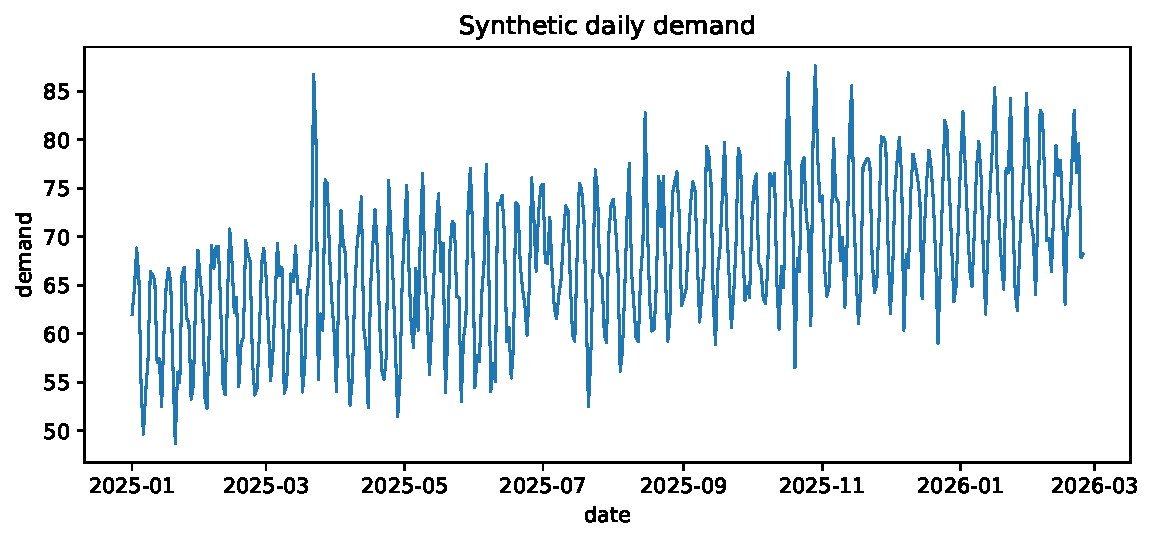
\includegraphics[keepaspectratio]{chapters/chapter-26-end-to-end-forecasting-pipeline_files/figure-pdf/py-ch26-simulate-demand-output-1.pdf}}

}

\caption{Synthetic daily demand with trend, weekly seasonality, and
occasional shocks.}

\end{figure}%

The variable \texttt{promo\_known} is treated as a known calendar-like
event. In a real project, a promotion indicator is valid only if the
promotion schedule is known at the forecast origin.

\section{26.14 Feature construction with explicit
timing}\label{feature-construction-with-explicit-timing}

The feature table must use past target values only.

\begin{Shaded}
\begin{Highlighting}[]
\ImportTok{from}\NormalTok{ sklearn.preprocessing }\ImportTok{import}\NormalTok{ StandardScaler}
\ImportTok{from}\NormalTok{ sklearn.linear\_model }\ImportTok{import}\NormalTok{ Ridge}
\ImportTok{from}\NormalTok{ sklearn.ensemble }\ImportTok{import}\NormalTok{ GradientBoostingRegressor}
\ImportTok{from}\NormalTok{ sklearn.pipeline }\ImportTok{import}\NormalTok{ Pipeline}
\ImportTok{from}\NormalTok{ sklearn.metrics }\ImportTok{import}\NormalTok{ mean\_absolute\_error, mean\_squared\_error}


\KeywordTok{def}\NormalTok{ make\_features(data, lags}\OperatorTok{=}\NormalTok{(}\DecValTok{1}\NormalTok{, }\DecValTok{7}\NormalTok{, }\DecValTok{14}\NormalTok{), rolling\_windows}\OperatorTok{=}\NormalTok{(}\DecValTok{7}\NormalTok{, }\DecValTok{14}\NormalTok{)):}
    \CommentTok{"""Create leakage{-}safe one{-}step{-}ahead features for predicting y\_t.}

\CommentTok{    Every target{-}derived feature for row t uses only y\_\{t{-}1\}, y\_\{t{-}2\}, ... .}
\CommentTok{    """}
\NormalTok{    out }\OperatorTok{=}\NormalTok{ pd.DataFrame(index}\OperatorTok{=}\NormalTok{data.index)}
\NormalTok{    y }\OperatorTok{=}\NormalTok{ data[}\StringTok{"y"}\NormalTok{]}

    \ControlFlowTok{for}\NormalTok{ lag }\KeywordTok{in}\NormalTok{ lags:}
\NormalTok{        out[}\SpecialStringTok{f"lag\_}\SpecialCharTok{\{}\NormalTok{lag}\SpecialCharTok{\}}\SpecialStringTok{"}\NormalTok{] }\OperatorTok{=}\NormalTok{ y.shift(lag)}

    \ControlFlowTok{for}\NormalTok{ window }\KeywordTok{in}\NormalTok{ rolling\_windows:}
\NormalTok{        out[}\SpecialStringTok{f"roll\_mean\_}\SpecialCharTok{\{}\NormalTok{window}\SpecialCharTok{\}}\SpecialStringTok{"}\NormalTok{] }\OperatorTok{=}\NormalTok{ y.shift(}\DecValTok{1}\NormalTok{).rolling(window).mean()}
\NormalTok{        out[}\SpecialStringTok{f"roll\_std\_}\SpecialCharTok{\{}\NormalTok{window}\SpecialCharTok{\}}\SpecialStringTok{"}\NormalTok{] }\OperatorTok{=}\NormalTok{ y.shift(}\DecValTok{1}\NormalTok{).rolling(window).std()}

\NormalTok{    day }\OperatorTok{=}\NormalTok{ data[}\StringTok{"ds"}\NormalTok{].dt.dayofweek.to\_numpy()}
\NormalTok{    out[}\StringTok{"dow\_sin"}\NormalTok{] }\OperatorTok{=}\NormalTok{ np.sin(}\DecValTok{2} \OperatorTok{*}\NormalTok{ np.pi }\OperatorTok{*}\NormalTok{ day }\OperatorTok{/} \DecValTok{7}\NormalTok{)}
\NormalTok{    out[}\StringTok{"dow\_cos"}\NormalTok{] }\OperatorTok{=}\NormalTok{ np.cos(}\DecValTok{2} \OperatorTok{*}\NormalTok{ np.pi }\OperatorTok{*}\NormalTok{ day }\OperatorTok{/} \DecValTok{7}\NormalTok{)}
\NormalTok{    out[}\StringTok{"trend"}\NormalTok{] }\OperatorTok{=}\NormalTok{ np.arange(}\BuiltInTok{len}\NormalTok{(data))}
\NormalTok{    out[}\StringTok{"promo\_known"}\NormalTok{] }\OperatorTok{=}\NormalTok{ data[}\StringTok{"promo\_known"}\NormalTok{].astype(}\BuiltInTok{float}\NormalTok{)}
\NormalTok{    out[}\StringTok{"target"}\NormalTok{] }\OperatorTok{=}\NormalTok{ y}
\NormalTok{    out[}\StringTok{"ds"}\NormalTok{] }\OperatorTok{=}\NormalTok{ data[}\StringTok{"ds"}\NormalTok{]}

    \ControlFlowTok{return}\NormalTok{ out.dropna().reset\_index(drop}\OperatorTok{=}\VariableTok{True}\NormalTok{)}

\NormalTok{feature\_df }\OperatorTok{=}\NormalTok{ make\_features(df)}
\NormalTok{feature\_cols }\OperatorTok{=}\NormalTok{ [c }\ControlFlowTok{for}\NormalTok{ c }\KeywordTok{in}\NormalTok{ feature\_df.columns }\ControlFlowTok{if}\NormalTok{ c }\KeywordTok{not} \KeywordTok{in}\NormalTok{ [}\StringTok{"target"}\NormalTok{, }\StringTok{"ds"}\NormalTok{]]}

\NormalTok{feature\_df.head()}
\end{Highlighting}
\end{Shaded}

\protect\phantomsection\label{py-ch26-feature-builder}
{\def\LTcaptype{none} % do not increment counter
\begin{longtable}[]{@{}llllllllllllll@{}}
\toprule\noalign{}
& lag\_1 & lag\_7 & lag\_14 & roll\_mean\_7 & roll\_std\_7 &
roll\_mean\_14 & roll\_std\_14 & dow\_sin & dow\_cos & trend &
promo\_known & target & ds \\
\midrule\noalign{}
\endhead
\bottomrule\noalign{}
\endlastfoot
0 & 52.486262 & 57.317373 & 61.993909 & 60.320347 & 5.578485 & 60.084311
& 6.204204 & 0.974928 & -0.222521 & 14 & 0.0 & 59.907672 & 2025-01-15 \\
1 & 59.907672 & 66.391572 & 64.693202 & 60.690390 & 5.430023 & 59.935294
& 6.179817 & 0.433884 & -0.900969 & 15 & 0.0 & 64.921686 & 2025-01-16 \\
2 & 64.921686 & 66.125463 & 68.841626 & 60.480406 & 5.196195 & 59.951614
& 6.193635 & -0.433884 & -0.900969 & 16 & 0.0 & 66.696564 &
2025-01-17 \\
3 & 66.696564 & 65.472355 & 65.610715 & 60.561992 & 5.302986 & 59.798395
& 5.979631 & -0.974928 & -0.222521 & 17 & 0.0 & 65.268535 &
2025-01-18 \\
4 & 65.268535 & 57.054627 & 54.062290 & 60.532875 & 5.272000 & 59.773954
& 5.954693 & -0.781831 & 0.623490 & 18 & 0.0 & 56.411896 & 2025-01-19 \\
\end{longtable}
}

A useful habit is to test the feature timing directly.

\protect\phantomsection\label{py-ch26-feature-timing-test}
\begin{Shaded}
\begin{Highlighting}[]
\CommentTok{\# For a selected row, verify that roll\_mean\_7 equals the mean of the previous seven y{-}values.}
\NormalTok{row }\OperatorTok{=} \DecValTok{25}
\NormalTok{original\_position }\OperatorTok{=}\NormalTok{ row }\OperatorTok{+} \DecValTok{14}  \CommentTok{\# because dropna removes the first 14 rows}
\NormalTok{manual }\OperatorTok{=}\NormalTok{ df.loc[original\_position}\OperatorTok{{-}}\DecValTok{7}\NormalTok{:original\_position}\OperatorTok{{-}}\DecValTok{1}\NormalTok{, }\StringTok{"y"}\NormalTok{].mean()}
\NormalTok{computed }\OperatorTok{=}\NormalTok{ feature\_df.loc[row, }\StringTok{"roll\_mean\_7"}\NormalTok{]}

\BuiltInTok{print}\NormalTok{(}\StringTok{"manual previous{-}7 mean:"}\NormalTok{, }\BuiltInTok{round}\NormalTok{(manual, }\DecValTok{4}\NormalTok{))}
\BuiltInTok{print}\NormalTok{(}\StringTok{"computed feature:"}\NormalTok{, }\BuiltInTok{round}\NormalTok{(computed, }\DecValTok{4}\NormalTok{))}
\ControlFlowTok{assert}\NormalTok{ np.isclose(manual, computed)}
\end{Highlighting}
\end{Shaded}

\begin{verbatim}
manual previous-7 mean: 62.8895
computed feature: 62.8895
\end{verbatim}

\section{26.15 Chronological holdout and
baselines}\label{chronological-holdout-and-baselines}

We first create a chronological split and evaluate simple baselines.

\begin{Shaded}
\begin{Highlighting}[]
\NormalTok{split }\OperatorTok{=} \BuiltInTok{int}\NormalTok{(}\FloatTok{0.75} \OperatorTok{*} \BuiltInTok{len}\NormalTok{(feature\_df))}
\NormalTok{train }\OperatorTok{=}\NormalTok{ feature\_df.iloc[:split].copy()}
\NormalTok{test }\OperatorTok{=}\NormalTok{ feature\_df.iloc[split:].copy()}

\NormalTok{y\_train }\OperatorTok{=}\NormalTok{ train[}\StringTok{"target"}\NormalTok{].to\_numpy()}
\NormalTok{y\_test }\OperatorTok{=}\NormalTok{ test[}\StringTok{"target"}\NormalTok{].to\_numpy()}

\NormalTok{baseline\_preds }\OperatorTok{=}\NormalTok{ pd.DataFrame(\{}
    \StringTok{"ds"}\NormalTok{: test[}\StringTok{"ds"}\NormalTok{],}
    \StringTok{"actual"}\NormalTok{: y\_test,}
    \StringTok{"naive\_lag\_1"}\NormalTok{: test[}\StringTok{"lag\_1"}\NormalTok{],}
    \StringTok{"seasonal\_naive\_lag\_7"}\NormalTok{: test[}\StringTok{"lag\_7"}\NormalTok{],}
    \StringTok{"rolling\_mean\_7"}\NormalTok{: test[}\StringTok{"roll\_mean\_7"}\NormalTok{],}
\NormalTok{\})}


\KeywordTok{def}\NormalTok{ rmse(y\_true, y\_pred):}
    \ControlFlowTok{return}\NormalTok{ mean\_squared\_error(y\_true, y\_pred) }\OperatorTok{**} \FloatTok{0.5}

\NormalTok{baseline\_summary }\OperatorTok{=}\NormalTok{ []}
\ControlFlowTok{for}\NormalTok{ col }\KeywordTok{in}\NormalTok{ [}\StringTok{"naive\_lag\_1"}\NormalTok{, }\StringTok{"seasonal\_naive\_lag\_7"}\NormalTok{, }\StringTok{"rolling\_mean\_7"}\NormalTok{]:}
\NormalTok{    baseline\_summary.append(\{}
        \StringTok{"model"}\NormalTok{: col,}
        \StringTok{"MAE"}\NormalTok{: mean\_absolute\_error(y\_test, baseline\_preds[col]),}
        \StringTok{"RMSE"}\NormalTok{: rmse(y\_test, baseline\_preds[col]),}
\NormalTok{    \})}

\NormalTok{pd.DataFrame(baseline\_summary).sort\_values(}\StringTok{"MAE"}\NormalTok{)}
\end{Highlighting}
\end{Shaded}

\protect\phantomsection\label{py-ch26-holdout-baselines}
{\def\LTcaptype{none} % do not increment counter
\begin{longtable}[]{@{}llll@{}}
\toprule\noalign{}
& model & MAE & RMSE \\
\midrule\noalign{}
\endhead
\bottomrule\noalign{}
\endlastfoot
1 & seasonal\_naive\_lag\_7 & 3.259153 & 4.056401 \\
0 & naive\_lag\_1 & 5.391515 & 6.321787 \\
2 & rolling\_mean\_7 & 5.559941 & 6.449090 \\
\end{longtable}
}

\section{26.16 Candidate models inside preprocessing
pipelines}\label{candidate-models-inside-preprocessing-pipelines}

Scaling must be fitted on training data only. \texttt{scikit-learn}
pipelines help enforce this rule.

\begin{Shaded}
\begin{Highlighting}[]
\NormalTok{X\_train }\OperatorTok{=}\NormalTok{ train[feature\_cols]}
\NormalTok{X\_test }\OperatorTok{=}\NormalTok{ test[feature\_cols]}

\NormalTok{models }\OperatorTok{=}\NormalTok{ \{}
    \StringTok{"ridge"}\NormalTok{: Pipeline([}
\NormalTok{        (}\StringTok{"scaler"}\NormalTok{, StandardScaler()),}
\NormalTok{        (}\StringTok{"model"}\NormalTok{, Ridge(alpha}\OperatorTok{=}\FloatTok{5.0}\NormalTok{))}
\NormalTok{    ]),}
    \StringTok{"gradient\_boosting"}\NormalTok{: GradientBoostingRegressor(}
\NormalTok{        n\_estimators}\OperatorTok{=}\DecValTok{60}\NormalTok{,}
\NormalTok{        learning\_rate}\OperatorTok{=}\FloatTok{0.05}\NormalTok{,}
\NormalTok{        max\_depth}\OperatorTok{=}\DecValTok{2}\NormalTok{,}
\NormalTok{        random\_state}\OperatorTok{=}\DecValTok{7339}\NormalTok{,}
\NormalTok{    ),}
\NormalTok{\}}

\NormalTok{model\_summary }\OperatorTok{=}\NormalTok{ []}
\NormalTok{predictions }\OperatorTok{=}\NormalTok{ baseline\_preds[[}\StringTok{"ds"}\NormalTok{, }\StringTok{"actual"}\NormalTok{]].copy()}

\ControlFlowTok{for}\NormalTok{ name, model }\KeywordTok{in}\NormalTok{ models.items():}
\NormalTok{    model.fit(X\_train, y\_train)}
\NormalTok{    pred }\OperatorTok{=}\NormalTok{ model.predict(X\_test)}
\NormalTok{    predictions[name] }\OperatorTok{=}\NormalTok{ pred}
\NormalTok{    model\_summary.append(\{}
        \StringTok{"model"}\NormalTok{: name,}
        \StringTok{"MAE"}\NormalTok{: mean\_absolute\_error(y\_test, pred),}
        \StringTok{"RMSE"}\NormalTok{: rmse(y\_test, pred),}
\NormalTok{    \})}

\NormalTok{all\_results }\OperatorTok{=}\NormalTok{ pd.concat([}
\NormalTok{    pd.DataFrame(baseline\_summary),}
\NormalTok{    pd.DataFrame(model\_summary)}
\NormalTok{], ignore\_index}\OperatorTok{=}\VariableTok{True}\NormalTok{).sort\_values(}\StringTok{"MAE"}\NormalTok{)}

\NormalTok{all\_results}
\end{Highlighting}
\end{Shaded}

\protect\phantomsection\label{py-ch26-fit-candidate-models}
{\def\LTcaptype{none} % do not increment counter
\begin{longtable}[]{@{}llll@{}}
\toprule\noalign{}
& model & MAE & RMSE \\
\midrule\noalign{}
\endhead
\bottomrule\noalign{}
\endlastfoot
3 & ridge & 2.125771 & 2.727825 \\
1 & seasonal\_naive\_lag\_7 & 3.259153 & 4.056401 \\
4 & gradient\_boosting & 3.305782 & 4.089745 \\
0 & naive\_lag\_1 & 5.391515 & 6.321787 \\
2 & rolling\_mean\_7 & 5.559941 & 6.449090 \\
\end{longtable}
}

\begin{Shaded}
\begin{Highlighting}[]
\NormalTok{fig, ax }\OperatorTok{=}\NormalTok{ plt.subplots(figsize}\OperatorTok{=}\NormalTok{(}\DecValTok{9}\NormalTok{, }\FloatTok{3.8}\NormalTok{))}
\NormalTok{ax.plot(predictions[}\StringTok{"ds"}\NormalTok{], predictions[}\StringTok{"actual"}\NormalTok{], label}\OperatorTok{=}\StringTok{"actual"}\NormalTok{, linewidth}\OperatorTok{=}\FloatTok{1.5}\NormalTok{)}
\NormalTok{ax.plot(predictions[}\StringTok{"ds"}\NormalTok{], baseline\_preds[}\StringTok{"seasonal\_naive\_lag\_7"}\NormalTok{], label}\OperatorTok{=}\StringTok{"seasonal naive"}\NormalTok{, alpha}\OperatorTok{=}\FloatTok{0.8}\NormalTok{)}
\NormalTok{ax.plot(predictions[}\StringTok{"ds"}\NormalTok{], predictions[}\StringTok{"ridge"}\NormalTok{], label}\OperatorTok{=}\StringTok{"ridge"}\NormalTok{, alpha}\OperatorTok{=}\FloatTok{0.8}\NormalTok{)}
\NormalTok{ax.plot(predictions[}\StringTok{"ds"}\NormalTok{], predictions[}\StringTok{"gradient\_boosting"}\NormalTok{], label}\OperatorTok{=}\StringTok{"gradient boosting"}\NormalTok{, alpha}\OperatorTok{=}\FloatTok{0.8}\NormalTok{)}
\NormalTok{ax.set\_title(}\StringTok{"Holdout forecasts"}\NormalTok{)}
\NormalTok{ax.set\_xlabel(}\StringTok{"date"}\NormalTok{)}
\NormalTok{ax.set\_ylabel(}\StringTok{"demand"}\NormalTok{)}
\NormalTok{ax.legend()}
\NormalTok{plt.show()}
\end{Highlighting}
\end{Shaded}

\begin{figure}[H]

{\centering \pandocbounded{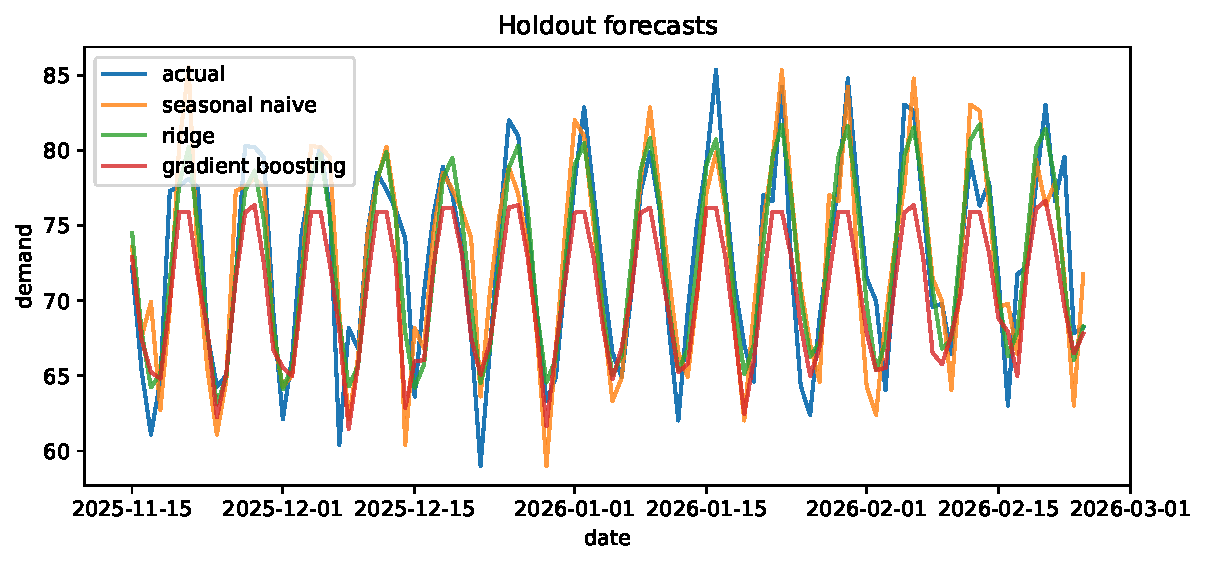
\includegraphics[keepaspectratio]{chapters/chapter-26-end-to-end-forecasting-pipeline_files/figure-pdf/py-ch26-plot-holdout-forecasts-output-1.pdf}}

}

\caption{Chronological test-set forecasts from baselines and
machine-learning models.}

\end{figure}%

\section{26.17 Rolling-origin
validation}\label{rolling-origin-validation}

A single holdout split can be misleading. We next run rolling
one-step-ahead validation. Each split trains on all earlier rows and
predicts the next row.

\begin{Shaded}
\begin{Highlighting}[]
\KeywordTok{def}\NormalTok{ rolling\_one\_step\_scores(feature\_data, feature\_cols, model\_factory, min\_train}\OperatorTok{=}\DecValTok{180}\NormalTok{, step}\OperatorTok{=}\DecValTok{7}\NormalTok{):}
\NormalTok{    records }\OperatorTok{=}\NormalTok{ []}
    \ControlFlowTok{for}\NormalTok{ end }\KeywordTok{in} \BuiltInTok{range}\NormalTok{(min\_train, }\BuiltInTok{len}\NormalTok{(feature\_data) }\OperatorTok{{-}} \DecValTok{1}\NormalTok{, step):}
\NormalTok{        train\_part }\OperatorTok{=}\NormalTok{ feature\_data.iloc[:end]}
\NormalTok{        test\_row }\OperatorTok{=}\NormalTok{ feature\_data.iloc[[end]]}

\NormalTok{        X\_tr }\OperatorTok{=}\NormalTok{ train\_part[feature\_cols]}
\NormalTok{        y\_tr }\OperatorTok{=}\NormalTok{ train\_part[}\StringTok{"target"}\NormalTok{].to\_numpy()}
\NormalTok{        X\_te }\OperatorTok{=}\NormalTok{ test\_row[feature\_cols]}
\NormalTok{        y\_te }\OperatorTok{=}\NormalTok{ test\_row[}\StringTok{"target"}\NormalTok{].to\_numpy()}

\NormalTok{        model }\OperatorTok{=}\NormalTok{ model\_factory()}
\NormalTok{        model.fit(X\_tr, y\_tr)}
\NormalTok{        pred }\OperatorTok{=} \BuiltInTok{float}\NormalTok{(model.predict(X\_te)[}\DecValTok{0}\NormalTok{])}

\NormalTok{        records.append(\{}
            \StringTok{"ds"}\NormalTok{: test\_row[}\StringTok{"ds"}\NormalTok{].iloc[}\DecValTok{0}\NormalTok{],}
            \StringTok{"actual"}\NormalTok{: }\BuiltInTok{float}\NormalTok{(y\_te[}\DecValTok{0}\NormalTok{]),}
            \StringTok{"prediction"}\NormalTok{: pred,}
            \StringTok{"error"}\NormalTok{: }\BuiltInTok{float}\NormalTok{(y\_te[}\DecValTok{0}\NormalTok{] }\OperatorTok{{-}}\NormalTok{ pred),}
\NormalTok{        \})}
    \ControlFlowTok{return}\NormalTok{ pd.DataFrame(records)}

\NormalTok{ridge\_factory }\OperatorTok{=} \KeywordTok{lambda}\NormalTok{: Pipeline([}
\NormalTok{    (}\StringTok{"scaler"}\NormalTok{, StandardScaler()),}
\NormalTok{    (}\StringTok{"model"}\NormalTok{, Ridge(alpha}\OperatorTok{=}\FloatTok{5.0}\NormalTok{))}
\NormalTok{])}

\NormalTok{gb\_factory }\OperatorTok{=} \KeywordTok{lambda}\NormalTok{: GradientBoostingRegressor(}
\NormalTok{    n\_estimators}\OperatorTok{=}\DecValTok{60}\NormalTok{,}
\NormalTok{    learning\_rate}\OperatorTok{=}\FloatTok{0.05}\NormalTok{,}
\NormalTok{    max\_depth}\OperatorTok{=}\DecValTok{2}\NormalTok{,}
\NormalTok{    random\_state}\OperatorTok{=}\DecValTok{7339}\NormalTok{,}
\NormalTok{)}

\NormalTok{ridge\_roll }\OperatorTok{=}\NormalTok{ rolling\_one\_step\_scores(feature\_df, feature\_cols, ridge\_factory)}
\NormalTok{gb\_roll }\OperatorTok{=}\NormalTok{ rolling\_one\_step\_scores(feature\_df, feature\_cols, gb\_factory)}

\NormalTok{rolling\_summary }\OperatorTok{=}\NormalTok{ pd.DataFrame([}
\NormalTok{    \{}\StringTok{"model"}\NormalTok{: }\StringTok{"ridge rolling"}\NormalTok{, }\StringTok{"MAE"}\NormalTok{: mean\_absolute\_error(ridge\_roll[}\StringTok{"actual"}\NormalTok{], ridge\_roll[}\StringTok{"prediction"}\NormalTok{]), }\StringTok{"RMSE"}\NormalTok{: rmse(ridge\_roll[}\StringTok{"actual"}\NormalTok{], ridge\_roll[}\StringTok{"prediction"}\NormalTok{])\},}
\NormalTok{    \{}\StringTok{"model"}\NormalTok{: }\StringTok{"gradient boosting rolling"}\NormalTok{, }\StringTok{"MAE"}\NormalTok{: mean\_absolute\_error(gb\_roll[}\StringTok{"actual"}\NormalTok{], gb\_roll[}\StringTok{"prediction"}\NormalTok{]), }\StringTok{"RMSE"}\NormalTok{: rmse(gb\_roll[}\StringTok{"actual"}\NormalTok{], gb\_roll[}\StringTok{"prediction"}\NormalTok{])\},}
\NormalTok{])}

\NormalTok{rolling\_summary}
\end{Highlighting}
\end{Shaded}

\protect\phantomsection\label{py-ch26-rolling-origin-function}
{\def\LTcaptype{none} % do not increment counter
\begin{longtable}[]{@{}llll@{}}
\toprule\noalign{}
& model & MAE & RMSE \\
\midrule\noalign{}
\endhead
\bottomrule\noalign{}
\endlastfoot
0 & ridge rolling & 2.527239 & 3.151755 \\
1 & gradient boosting rolling & 2.942416 & 3.588993 \\
\end{longtable}
}

\begin{Shaded}
\begin{Highlighting}[]
\NormalTok{fig, ax }\OperatorTok{=}\NormalTok{ plt.subplots(figsize}\OperatorTok{=}\NormalTok{(}\DecValTok{9}\NormalTok{, }\FloatTok{3.5}\NormalTok{))}
\NormalTok{ax.axhline(}\DecValTok{0}\NormalTok{, linewidth}\OperatorTok{=}\DecValTok{1}\NormalTok{)}
\NormalTok{ax.plot(ridge\_roll[}\StringTok{"ds"}\NormalTok{], ridge\_roll[}\StringTok{"error"}\NormalTok{], marker}\OperatorTok{=}\StringTok{"o"}\NormalTok{, markersize}\OperatorTok{=}\DecValTok{3}\NormalTok{, label}\OperatorTok{=}\StringTok{"ridge error"}\NormalTok{)}
\NormalTok{ax.plot(gb\_roll[}\StringTok{"ds"}\NormalTok{], gb\_roll[}\StringTok{"error"}\NormalTok{], marker}\OperatorTok{=}\StringTok{"o"}\NormalTok{, markersize}\OperatorTok{=}\DecValTok{3}\NormalTok{, label}\OperatorTok{=}\StringTok{"gradient boosting error"}\NormalTok{)}
\NormalTok{ax.set\_title(}\StringTok{"Rolling{-}origin one{-}step forecast errors"}\NormalTok{)}
\NormalTok{ax.set\_xlabel(}\StringTok{"date"}\NormalTok{)}
\NormalTok{ax.set\_ylabel(}\StringTok{"error"}\NormalTok{)}
\NormalTok{ax.legend()}
\NormalTok{plt.show()}
\end{Highlighting}
\end{Shaded}

\begin{figure}[H]

{\centering \pandocbounded{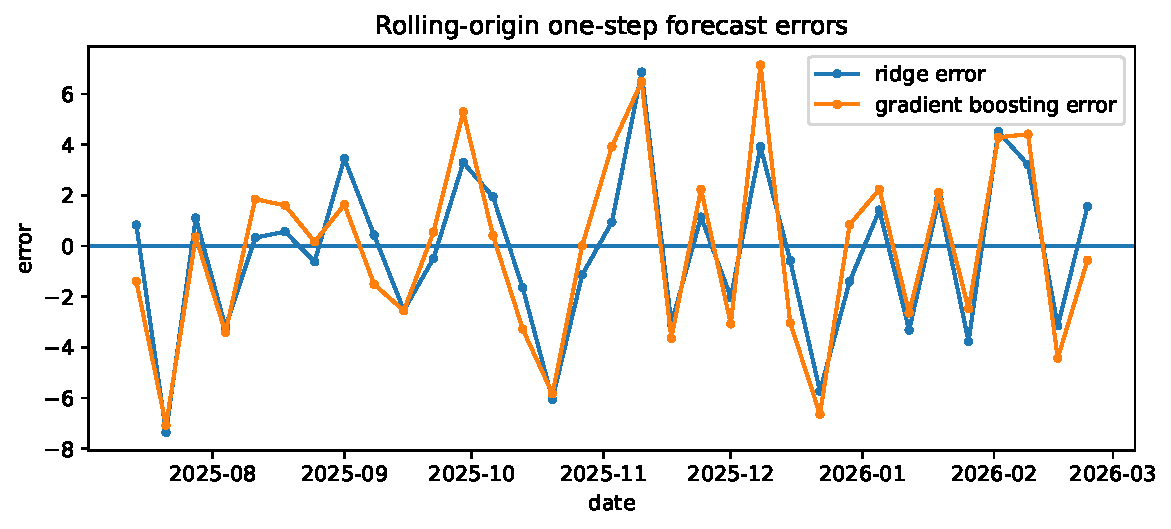
\includegraphics[keepaspectratio]{chapters/chapter-26-end-to-end-forecasting-pipeline_files/figure-pdf/py-ch26-rolling-error-plot-output-1.pdf}}

}

\caption{Rolling one-step-ahead forecast errors.}

\end{figure}%

\section{26.18 Residual-based interval
construction}\label{residual-based-interval-construction}

We can construct a simple validation-residual interval. This is not the
only approach, but it is transparent.

\begin{Shaded}
\begin{Highlighting}[]
\CommentTok{\# Fit the selected model on the chronological training set.}
\NormalTok{selected }\OperatorTok{=}\NormalTok{ Pipeline([}
\NormalTok{    (}\StringTok{"scaler"}\NormalTok{, StandardScaler()),}
\NormalTok{    (}\StringTok{"model"}\NormalTok{, Ridge(alpha}\OperatorTok{=}\FloatTok{5.0}\NormalTok{))}
\NormalTok{])}
\NormalTok{selected.fit(X\_train, y\_train)}
\NormalTok{point\_pred }\OperatorTok{=}\NormalTok{ selected.predict(X\_test)}

\CommentTok{\# Use rolling{-}origin residual quantiles as empirical error offsets.}
\NormalTok{residuals }\OperatorTok{=}\NormalTok{ ridge\_roll[}\StringTok{"error"}\NormalTok{].to\_numpy()}
\NormalTok{lo\_offset, hi\_offset }\OperatorTok{=}\NormalTok{ np.quantile(residuals, [}\FloatTok{0.05}\NormalTok{, }\FloatTok{0.95}\NormalTok{])}

\NormalTok{interval\_df }\OperatorTok{=}\NormalTok{ pd.DataFrame(\{}
    \StringTok{"ds"}\NormalTok{: test[}\StringTok{"ds"}\NormalTok{],}
    \StringTok{"actual"}\NormalTok{: y\_test,}
    \StringTok{"forecast"}\NormalTok{: point\_pred,}
    \StringTok{"lower\_90"}\NormalTok{: point\_pred }\OperatorTok{+}\NormalTok{ lo\_offset,}
    \StringTok{"upper\_90"}\NormalTok{: point\_pred }\OperatorTok{+}\NormalTok{ hi\_offset,}
\NormalTok{\})}

\NormalTok{coverage }\OperatorTok{=}\NormalTok{ np.mean((interval\_df[}\StringTok{"actual"}\NormalTok{] }\OperatorTok{\textgreater{}=}\NormalTok{ interval\_df[}\StringTok{"lower\_90"}\NormalTok{]) }\OperatorTok{\&}\NormalTok{ (interval\_df[}\StringTok{"actual"}\NormalTok{] }\OperatorTok{\textless{}=}\NormalTok{ interval\_df[}\StringTok{"upper\_90"}\NormalTok{]))}
\BuiltInTok{print}\NormalTok{(}\StringTok{"Empirical 90}\SpecialCharTok{\% i}\StringTok{nterval coverage on holdout:"}\NormalTok{, }\BuiltInTok{round}\NormalTok{(coverage, }\DecValTok{3}\NormalTok{))}
\NormalTok{interval\_df.head()}
\end{Highlighting}
\end{Shaded}

\begin{verbatim}
Empirical 90% interval coverage on holdout: 0.912
\end{verbatim}

\protect\phantomsection\label{py-ch26-residual-interval}
{\def\LTcaptype{none} % do not increment counter
\begin{longtable}[]{@{}llllll@{}}
\toprule\noalign{}
& ds & actual & forecast & lower\_90 & upper\_90 \\
\midrule\noalign{}
\endhead
\bottomrule\noalign{}
\endlastfoot
304 & 2025-11-15 & 72.215943 & 74.524246 & 68.666280 & 78.673867 \\
305 & 2025-11-16 & 65.376446 & 67.945236 & 62.087271 & 72.094857 \\
306 & 2025-11-17 & 61.087872 & 64.236849 & 58.378883 & 68.386469 \\
307 & 2025-11-18 & 64.692912 & 65.150766 & 59.292800 & 69.300386 \\
308 & 2025-11-19 & 77.285982 & 71.310223 & 65.452257 & 75.459843 \\
\end{longtable}
}

\begin{Shaded}
\begin{Highlighting}[]
\NormalTok{fig, ax }\OperatorTok{=}\NormalTok{ plt.subplots(figsize}\OperatorTok{=}\NormalTok{(}\DecValTok{9}\NormalTok{, }\FloatTok{3.8}\NormalTok{))}
\NormalTok{ax.plot(interval\_df[}\StringTok{"ds"}\NormalTok{], interval\_df[}\StringTok{"actual"}\NormalTok{], label}\OperatorTok{=}\StringTok{"actual"}\NormalTok{, linewidth}\OperatorTok{=}\FloatTok{1.3}\NormalTok{)}
\NormalTok{ax.plot(interval\_df[}\StringTok{"ds"}\NormalTok{], interval\_df[}\StringTok{"forecast"}\NormalTok{], label}\OperatorTok{=}\StringTok{"forecast"}\NormalTok{, linewidth}\OperatorTok{=}\FloatTok{1.3}\NormalTok{)}
\NormalTok{ax.fill\_between(}
\NormalTok{    interval\_df[}\StringTok{"ds"}\NormalTok{],}
\NormalTok{    interval\_df[}\StringTok{"lower\_90"}\NormalTok{].to\_numpy(),}
\NormalTok{    interval\_df[}\StringTok{"upper\_90"}\NormalTok{].to\_numpy(),}
\NormalTok{    alpha}\OperatorTok{=}\FloatTok{0.2}\NormalTok{,}
\NormalTok{    label}\OperatorTok{=}\StringTok{"90}\SpecialCharTok{\% r}\StringTok{esidual interval"}\NormalTok{,}
\NormalTok{)}
\NormalTok{ax.set\_title(}\StringTok{"Forecast report object: point forecast and interval"}\NormalTok{)}
\NormalTok{ax.set\_xlabel(}\StringTok{"date"}\NormalTok{)}
\NormalTok{ax.set\_ylabel(}\StringTok{"demand"}\NormalTok{)}
\NormalTok{ax.legend()}
\NormalTok{plt.show()}
\end{Highlighting}
\end{Shaded}

\begin{figure}[H]

{\centering \pandocbounded{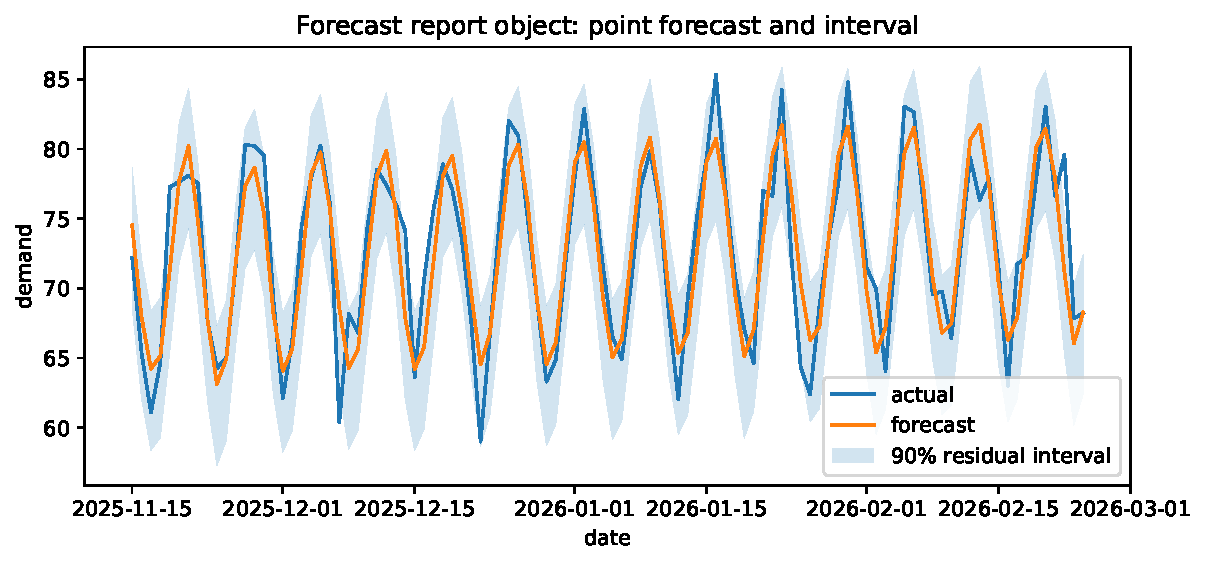
\includegraphics[keepaspectratio]{chapters/chapter-26-end-to-end-forecasting-pipeline_files/figure-pdf/py-ch26-interval-plot-output-1.pdf}}

}

\caption{Point forecasts with a residual-quantile interval.}

\end{figure}%

\section{26.19 Final forecast report
object}\label{final-forecast-report-object}

A final forecast should be saved as a table with enough metadata to be
interpreted later.

\begin{Shaded}
\begin{Highlighting}[]
\NormalTok{forecast\_origin }\OperatorTok{=}\NormalTok{ train[}\StringTok{"ds"}\NormalTok{].}\BuiltInTok{max}\NormalTok{()}
\NormalTok{report }\OperatorTok{=}\NormalTok{ interval\_df.copy()}
\NormalTok{report[}\StringTok{"forecast\_origin"}\NormalTok{] }\OperatorTok{=}\NormalTok{ forecast\_origin}
\NormalTok{report[}\StringTok{"model"}\NormalTok{] }\OperatorTok{=} \StringTok{"ridge\_lag\_calendar\_pipeline"}
\NormalTok{report[}\StringTok{"target"}\NormalTok{] }\OperatorTok{=} \StringTok{"daily demand"}
\NormalTok{report[}\StringTok{"horizon\_days\_after\_origin"}\NormalTok{] }\OperatorTok{=}\NormalTok{ (report[}\StringTok{"ds"}\NormalTok{] }\OperatorTok{{-}}\NormalTok{ forecast\_origin).dt.days}

\NormalTok{report[[}\StringTok{"forecast\_origin"}\NormalTok{, }\StringTok{"ds"}\NormalTok{, }\StringTok{"horizon\_days\_after\_origin"}\NormalTok{, }\StringTok{"model"}\NormalTok{, }\StringTok{"forecast"}\NormalTok{, }\StringTok{"lower\_90"}\NormalTok{, }\StringTok{"upper\_90"}\NormalTok{]].head()}
\end{Highlighting}
\end{Shaded}

\protect\phantomsection\label{py-ch26-forecast-report-object}
{\def\LTcaptype{none} % do not increment counter
\begin{longtable}[]{@{}llllllll@{}}
\toprule\noalign{}
& forecast\_origin & ds & horizon\_days\_after\_origin & model &
forecast & lower\_90 & upper\_90 \\
\midrule\noalign{}
\endhead
\bottomrule\noalign{}
\endlastfoot
304 & 2025-11-14 & 2025-11-15 & 1 & ridge\_lag\_calendar\_pipeline &
74.524246 & 68.666280 & 78.673867 \\
305 & 2025-11-14 & 2025-11-16 & 2 & ridge\_lag\_calendar\_pipeline &
67.945236 & 62.087271 & 72.094857 \\
306 & 2025-11-14 & 2025-11-17 & 3 & ridge\_lag\_calendar\_pipeline &
64.236849 & 58.378883 & 68.386469 \\
307 & 2025-11-14 & 2025-11-18 & 4 & ridge\_lag\_calendar\_pipeline &
65.150766 & 59.292800 & 69.300386 \\
308 & 2025-11-14 & 2025-11-19 & 5 & ridge\_lag\_calendar\_pipeline &
71.310223 & 65.452257 & 75.459843 \\
\end{longtable}
}

The report object should be accompanied by a model card or modeling log.
A concise model card includes the forecast contract, training period,
validation design, model class, feature list, metrics, interval
coverage, known limitations, and monitoring plan.

\section{26.20 AI-assisted pipeline
review}\label{ai-assisted-pipeline-review}

\section{AI-assisted modeling
prompt}\label{ai-assisted-modeling-prompt-1}

Use this prompt after your first complete pipeline is working.

\begin{quote}
I am building a time-series forecasting pipeline. The target is
{[}target{]}. The frequency is {[}frequency{]}. The forecast horizon is
{[}horizon{]}. The information available at the forecast origin is
\hyperref[information-set]{information set}. My preprocessing steps are
{[}steps{]}. My features are {[}features{]}. My validation design is
{[}design{]}. My baselines are {[}baselines{]}. My candidate models are
{[}models{]}. My metrics are {[}metrics{]}. My residual diagnostics are
{[}diagnostics{]}. Please act as a skeptical reviewer. Identify possible
leakage, horizon mismatch, weak baselines, invalid transformations,
nonstationarity, calibration problems, and unsupported conclusions. For
every concern, give a concrete verification step.
\end{quote}

The strongest AI prompt does not ask for approval. It asks for failure
modes and checks.

\section{26.21 Common mistakes}\label{common-mistakes-25}

\begin{enumerate}
\def\labelenumi{\arabic{enumi}.}
\tightlist
\item
  \textbf{Building features before defining the forecast origin.} This
  often creates accidental future information.
\item
  \textbf{Using random splits.} Random splits break the time order and
  often overstate performance.
\item
  \textbf{Scaling before splitting.} Test-set information enters the
  training pipeline.
\item
  \textbf{Comparing advanced models without baselines.} A complex model
  should beat naive and seasonal-naive methods.
\item
  \textbf{Ignoring the horizon.} A model that predicts tomorrow may not
  predict next month.
\item
  \textbf{Using actual future lags in multi-step forecasting.} Recursive
  forecasts must use predicted values after the forecast origin.
\item
  \textbf{Reporting only one metric.} Use multiple metrics and
  horizon-wise summaries.
\item
  \textbf{Skipping monitoring.} A deployed forecast can degrade when the
  data-generating process changes.
\end{enumerate}

\section{26.22 Exercises}\label{exercises-25}

\begin{enumerate}
\def\labelenumi{\arabic{enumi}.}
\tightlist
\item
  Define a forecasting contract for weekly electricity demand with
  horizon \(H=4\) weeks. State the information set \(\mathcal F_t\).
\item
  For predicting \(Y_t\), decide whether each feature is valid:
  \(Y_{t-1}\), \(Y_{t+1}\), a centered seven-day rolling mean, a lagged
  seven-day rolling mean, day of week, and next week's temperature
  forecast.
\item
  Implement a leakage-safe feature table with lags \(1,2,7,14\) and
  rolling means of lengths \(7\) and \(28\).
\item
  Compare naive, seasonal naive, ridge regression, and gradient boosting
  using chronological validation.
\item
  Construct a residual-quantile interval and evaluate its empirical
  coverage.
\item
  Write a model card for your forecasting pipeline.
\item
  Modify the Python example so that it predicts seven days ahead.
  Explain how your validation design changes.
\item
  Create a synthetic distribution shift and design a monitoring
  statistic that detects it.
\end{enumerate}

\section{26.23 Mini project}\label{mini-project-8}

Choose a real or simulated time series. Build an end-to-end forecasting
pipeline with the following deliverables:

\begin{itemize}
\tightlist
\item
  a forecasting contract;
\item
  a leakage-safe feature table;
\item
  at least two baselines;
\item
  at least two candidate models;
\item
  chronological or rolling-origin validation;
\item
  point forecast metrics;
\item
  an interval or uncertainty estimate;
\item
  residual or error diagnostics;
\item
  a final forecast report table;
\item
  a short AI-assisted critique and your verification of the critique.
\end{itemize}

\section{26.24 Chapter checklist}\label{chapter-checklist-16}

Before moving to the final project studio, make sure you can answer yes
to each question.

\begin{itemize}
\tightlist
\item
  Did I define the forecast origin and horizon?
\item
  Did I define the information set \(\mathcal F_t\)?
\item
  Are all target-derived features lagged correctly?
\item
  Were preprocessing steps fitted only on training data?
\item
  Did I compare against naive and seasonal-naive baselines?
\item
  Does my validation design match the deployment use case?
\item
  Did I inspect residuals or forecast errors?
\item
  Did I evaluate uncertainty or interval coverage?
\item
  Did I create a forecast report object?
\item
  Did I document assumptions, limitations, and monitoring rules?
\end{itemize}

\chapter{Final Project Studio}\label{final-project-studio}

\textbf{Part VII. Responsible AI, Projects, and Deployment}\\
\textbf{Chapter goal:} design, execute, and communicate a rigorous final
project in modern time series analysis and sequence learning. The
project should connect mathematical assumptions, an information-set
formulation, leakage-safe validation, interpretable diagnostics,
uncertainty, reproducible Python code, interactive visualization, and
AI-assisted model criticism.

\section{Learning objectives}\label{learning-objectives-26}

After studying this chapter, you should be able to:

\begin{enumerate}
\def\labelenumi{\arabic{enumi}.}
\tightlist
\item
  translate an applied time-series or sequence-data question into a
  precise mathematical problem;
\item
  write a project contract specifying target, forecast origin, horizon,
  information set, loss, baselines, and deliverables;
\item
  select an appropriate method family from classical statistics,
  spectral analysis, feature-based ML, deep learning, or representation
  learning;
\item
  design a validation scheme that respects time ordering and prevents
  leakage;
\item
  evaluate point forecasts, probabilistic forecasts, classifications,
  anomaly scores, or learned representations;
\item
  build an interactive HTML component that helps explain the project
  idea;
\item
  use AI assistance for critique, code review, and communication while
  verifying all claims;
\item
  prepare a reproducible notebook and a clear written report.
\end{enumerate}

\section{27.1 What counts as a strong final
project?}\label{what-counts-as-a-strong-final-project}

A strong final project is not just a competition to obtain the smallest
error. It is a complete mathematical and computational argument. The
report should answer four questions:

\begin{enumerate}
\def\labelenumi{\arabic{enumi}.}
\tightlist
\item
  \textbf{What is the prediction or inference problem?}
\item
  \textbf{What information is available when the decision is made?}
\item
  \textbf{What model assumptions are being made?}
\item
  \textbf{What evidence supports or contradicts those assumptions?}
\end{enumerate}

The project may focus on forecasting, anomaly detection, sequence
classification, regime detection, multivariate modeling, spectral
analysis, representation learning, or an AI-assisted forecasting
workflow. In every case, the project should be organized around an
ordered data set

\[
\bigl\{(t_i, y_i, x_i): i=1,\ldots,n\bigr\},
\]

where \(t_i\) is the time or sequence index, \(y_i\) is the target or
response, and \(x_i\) is an optional vector of covariates.

A useful high-level template is

\[
\text{scientific question}
\longrightarrow
\text{statistical task}
\longrightarrow
\text{information set}
\longrightarrow
\text{model class}
\longrightarrow
\text{validation design}
\longrightarrow
\text{diagnostic evidence}.
\]

\begin{tcolorbox}[enhanced jigsaw, arc=.35mm, bottomrule=.15mm, bottomtitle=1mm, breakable, colback=white, colbacktitle=quarto-callout-tip-color!10!white, colframe=quarto-callout-tip-color-frame, coltitle=black, left=2mm, leftrule=.75mm, opacityback=0, opacitybacktitle=0.6, rightrule=.15mm, title=\textcolor{quarto-callout-tip-color}{\faLightbulb}\hspace{0.5em}{Project principle}, titlerule=0mm, toprule=.15mm, toptitle=1mm]

A final project should make it easy for another student to reproduce the
result and understand why the validation design is valid for ordered
data.

\end{tcolorbox}

\section{27.2 The project contract}\label{the-project-contract}

Before fitting any model, write a \textbf{project contract}. This is the
mathematical specification of the problem.

For forecasting, define the forecast target as

\[
Y_{t+h}, \qquad h\in \mathcal H,
\]

where \(t\) is the forecast origin and \(\mathcal H\) is the set of
horizons. The information available at the origin is the filtration or
information set

\[
\mathcal F_t
=
\sigma\bigl(Y_s, X_s, C_u: s\le t,\ u\le t+h\text{ and known at time }t\bigr),
\]

where \(C_u\) may include calendar variables known in advance. A valid
forecast must have the form

\[
\widehat Y_{t+h|t}=g_h(\mathcal F_t).
\]

If a variable is not known at time \(t\), it must not be used as a
feature for predicting \(Y_{t+h}\) unless a separate model forecasts
that variable first.

For sequence classification, define a sequence window

\[
\mathbf X_i=(X_{i,1},\ldots,X_{i,L_i})
\]

and a label \(Z_i\in\{1,\ldots,K\}\). A classifier has the form

\[
\widehat p_\theta(k\mid \mathbf X_i)
= P_\theta(Z_i=k\mid \mathbf X_i).
\]

For anomaly detection, define a score

\[
A_t=s(Y_t,Y_{t-1},\ldots,X_t,X_{t-1},\ldots),
\]

where larger values indicate stronger evidence against normal behavior.
A threshold rule has the form

\[
\widehat Z_t=\mathbf 1\{A_t>c\}.
\]

For representation learning, define an encoder

\[
z_t = e_\theta(W_t),
\]

where \(W_t=(Y_{t-L+1},\ldots,Y_t)\) is a time window. The
representation should be evaluated through a downstream task such as
clustering, classification, anomaly detection, or forecasting.

\section{27.3 Choosing the project
type}\label{choosing-the-project-type}

The project type should match the structure of the data and the
available time.

{\def\LTcaptype{none} % do not increment counter
\begin{longtable}[]{@{}
  >{\raggedright\arraybackslash}p{(\linewidth - 6\tabcolsep) * \real{0.2500}}
  >{\raggedright\arraybackslash}p{(\linewidth - 6\tabcolsep) * \real{0.2500}}
  >{\raggedright\arraybackslash}p{(\linewidth - 6\tabcolsep) * \real{0.2500}}
  >{\raggedright\arraybackslash}p{(\linewidth - 6\tabcolsep) * \real{0.2500}}@{}}
\toprule\noalign{}
\begin{minipage}[b]{\linewidth}\raggedright
Project type
\end{minipage} & \begin{minipage}[b]{\linewidth}\raggedright
Good data situation
\end{minipage} & \begin{minipage}[b]{\linewidth}\raggedright
Main output
\end{minipage} & \begin{minipage}[b]{\linewidth}\raggedright
Typical methods
\end{minipage} \\
\midrule\noalign{}
\endhead
\bottomrule\noalign{}
\endlastfoot
Forecasting & one or many ordered series & \(\widehat Y_{t+h|t}\) &
naive, ARIMA, SARIMA, Prophet, ML, neural nets \\
Probabilistic forecasting & decision requires uncertainty & intervals or
quantiles & bootstrap, conformal, Bayesian, quantile regression \\
Anomaly detection & rare unusual events & anomaly score \(A_t\) &
residual methods, autoencoders, isolation forests \\
Sequence classification & each sequence has a label & class probability
& feature extraction, CNN, RNN, transformer \\
Regime detection & hidden states or structural breaks & inferred state
\(S_t\) & HMM, state-space, change-point methods \\
Spectral analysis & oscillations are central & dominant frequencies &
periodogram, smoothing, wavelets \\
Representation learning & many windows or many series & embeddings
\(z_t\) & PCA, autoencoder, contrastive learning \\
Multivariate forecasting & many interacting variables & vector forecast
& VAR, dynamic regression, global ML \\
\end{longtable}
}

A good project is usually narrow enough to finish but rich enough to
demonstrate both theory and computation.

\begin{tcolorbox}[enhanced jigsaw, arc=.35mm, bottomrule=.15mm, bottomtitle=1mm, breakable, colback=white, colbacktitle=quarto-callout-warning-color!10!white, colframe=quarto-callout-warning-color-frame, coltitle=black, left=2mm, leftrule=.75mm, opacityback=0, opacitybacktitle=0.6, rightrule=.15mm, title=\textcolor{quarto-callout-warning-color}{\faExclamationTriangle}\hspace{0.5em}{Avoid a project that is too broad}, titlerule=0mm, toprule=.15mm, toptitle=1mm]

``Forecast the stock market using deep learning'' is too broad. A better
project is: ``Compare a naive baseline, ARIMA, and a lag-feature
gradient-boosting model for one-day-ahead realized volatility
forecasting on a fixed set of assets, evaluated by rolling-origin
validation.''

\end{tcolorbox}

\section{27.4 Interactive module: project design
matrix}\label{interactive-module-project-design-matrix}

Use this module to think about project scope. The plot is not a grade.
It is a planning tool. A project with high data complexity and high
model ambition requires more careful validation and stronger
reproducibility.

Interactive Module: Project Design Matrix

Adjust the design choices and inspect the resulting feasibility profile.

Data length
\protect\phantomsection\label{ch27_design_length_value}{1200} Number of
related series
\protect\phantomsection\label{ch27_design_series_value}{8} Missingness /
irregularity
\protect\phantomsection\label{ch27_design_missing_value}{0.10} Forecast
horizon or sequence length
\protect\phantomsection\label{ch27_design_horizon_value}{14} Model
family baseline + classical model feature-based ML deep sequence model
hybrid statistical + neural Uncertainty required? no prediction
intervals quantiles / probabilities

\protect\phantomsection\label{ch27_design_plot}

\section{27.5 Validation design}\label{validation-design-1}

For forecasting, validation should mimic deployment. Suppose
\(\mathcal T\) is the set of forecast origins and \(\mathcal H\) is the
set of horizons. For a loss function \(\ell\), the rolling-origin
validation error is

\[
\widehat R
=
\frac{1}{|\mathcal T||\mathcal H|}
\sum_{\tau\in\mathcal T}\sum_{h\in\mathcal H}
\ell\left(Y_{\tau+h},\widehat Y_{\tau+h|\tau}\right).
\]

A horizon-specific error is

\[
\widehat R_h
=
\frac{1}{|\mathcal T|}
\sum_{\tau\in\mathcal T}
\ell\left(Y_{\tau+h},\widehat Y_{\tau+h|\tau}\right).
\]

This matters because some models perform well for \(h=1\) but poorly for
longer horizons.

For sequence classification, use a split that respects grouping and
chronology. If windows overlap heavily, random window splitting can leak
nearly identical examples into training and test sets. If a sequence
belongs to a patient, asset, device, or user, the split should respect
that grouping.

For anomaly detection, avoid setting the threshold using future
anomalies unless that would also happen in deployment. If labeled
anomalies are scarce, use a validation period that is separated from the
final test period.

\section{27.6 Interactive module: rolling-origin
planner}\label{interactive-module-rolling-origin-planner}

Interactive Module: Rolling-Origin Validation Planner

Visualize how many backtesting forecasts your project will require.

Total observations \protect\phantomsection\label{ch27_roll_n_value}{360}
Initial training size
\protect\phantomsection\label{ch27_roll_train_value}{160} Maximum
horizon \protect\phantomsection\label{ch27_roll_horizon_value}{21} Step
between origins \protect\phantomsection\label{ch27_roll_step_value}{14}
Window type expanding sliding Sliding window length
\protect\phantomsection\label{ch27_roll_window_length_value}{140}

\protect\phantomsection\label{ch27_roll_plot}

\section{27.7 Baselines and model
comparison}\label{baselines-and-model-comparison}

Every project should include at least one baseline. Baselines are not
optional. They prevent students from mistaking complexity for
performance.

For a univariate forecasting project, common baselines include:

\[
\widehat Y_{t+h|t}^{\mathrm{naive}}=Y_t,
\]

and for seasonal data with period \(s\),

\[
\widehat Y_{t+h|t}^{\mathrm{seasonal}}=Y_{t+h-ks},
\]

where \(k\) is chosen so that \(t+h-ks\le t\).

For sequence classification, compare against majority-class prediction,
logistic regression on summary features, or a simple CNN before using a
large transformer. For anomaly detection, compare against a residual
threshold or rolling z-score before using an autoencoder.

A recommended project model ladder is:

\[
\text{baseline}
\rightarrow
\text{interpretable statistical model}
\rightarrow
\text{feature-based ML}
\rightarrow
\text{deep model, if justified}.
\]

The final model does not need to be the most complex model. It should be
the model best supported by validation and diagnostics.

\section{27.8 Python example: a small final-project
prototype}\label{python-example-a-small-final-project-prototype}

The following example simulates daily demand data, creates a
chronological split, evaluates naive and seasonal-naive baselines, and
fits a small lag-feature regression model. It illustrates the minimum
level of computational reproducibility expected in a project.

\begin{Shaded}
\begin{Highlighting}[]
\ImportTok{import}\NormalTok{ numpy }\ImportTok{as}\NormalTok{ np}
\ImportTok{import}\NormalTok{ pandas }\ImportTok{as}\NormalTok{ pd}
\ImportTok{import}\NormalTok{ matplotlib.pyplot }\ImportTok{as}\NormalTok{ plt}
\ImportTok{from}\NormalTok{ sklearn.linear\_model }\ImportTok{import}\NormalTok{ Ridge}
\ImportTok{from}\NormalTok{ sklearn.metrics }\ImportTok{import}\NormalTok{ mean\_absolute\_error, mean\_squared\_error}

\NormalTok{rng }\OperatorTok{=}\NormalTok{ np.random.default\_rng(}\DecValTok{7339}\NormalTok{)}

\NormalTok{n }\OperatorTok{=} \DecValTok{420}
\NormalTok{t }\OperatorTok{=}\NormalTok{ np.arange(n)}
\NormalTok{weekly }\OperatorTok{=} \DecValTok{8} \OperatorTok{*}\NormalTok{ np.sin(}\DecValTok{2} \OperatorTok{*}\NormalTok{ np.pi }\OperatorTok{*}\NormalTok{ t }\OperatorTok{/} \DecValTok{7}\NormalTok{)}
\NormalTok{annualish }\OperatorTok{=} \DecValTok{3} \OperatorTok{*}\NormalTok{ np.sin(}\DecValTok{2} \OperatorTok{*}\NormalTok{ np.pi }\OperatorTok{*}\NormalTok{ t }\OperatorTok{/} \DecValTok{90}\NormalTok{)}
\NormalTok{trend }\OperatorTok{=} \FloatTok{0.04} \OperatorTok{*}\NormalTok{ t}
\NormalTok{noise }\OperatorTok{=}\NormalTok{ rng.normal(}\DecValTok{0}\NormalTok{, }\FloatTok{2.0}\NormalTok{, size}\OperatorTok{=}\NormalTok{n)}
\NormalTok{y }\OperatorTok{=} \DecValTok{80} \OperatorTok{+}\NormalTok{ trend }\OperatorTok{+}\NormalTok{ weekly }\OperatorTok{+}\NormalTok{ annualish }\OperatorTok{+}\NormalTok{ noise}

\NormalTok{df }\OperatorTok{=}\NormalTok{ pd.DataFrame(\{}\StringTok{"t"}\NormalTok{: t, }\StringTok{"y"}\NormalTok{: y\})}
\ControlFlowTok{for}\NormalTok{ lag }\KeywordTok{in}\NormalTok{ [}\DecValTok{1}\NormalTok{, }\DecValTok{7}\NormalTok{, }\DecValTok{14}\NormalTok{, }\DecValTok{28}\NormalTok{]:}
\NormalTok{    df[}\SpecialStringTok{f"lag\_}\SpecialCharTok{\{}\NormalTok{lag}\SpecialCharTok{\}}\SpecialStringTok{"}\NormalTok{] }\OperatorTok{=}\NormalTok{ df[}\StringTok{"y"}\NormalTok{].shift(lag)}
\NormalTok{df[}\StringTok{"sin7"}\NormalTok{] }\OperatorTok{=}\NormalTok{ np.sin(}\DecValTok{2} \OperatorTok{*}\NormalTok{ np.pi }\OperatorTok{*}\NormalTok{ df[}\StringTok{"t"}\NormalTok{] }\OperatorTok{/} \DecValTok{7}\NormalTok{)}
\NormalTok{df[}\StringTok{"cos7"}\NormalTok{] }\OperatorTok{=}\NormalTok{ np.cos(}\DecValTok{2} \OperatorTok{*}\NormalTok{ np.pi }\OperatorTok{*}\NormalTok{ df[}\StringTok{"t"}\NormalTok{] }\OperatorTok{/} \DecValTok{7}\NormalTok{)}
\NormalTok{df }\OperatorTok{=}\NormalTok{ df.dropna().reset\_index(drop}\OperatorTok{=}\VariableTok{True}\NormalTok{)}

\NormalTok{train\_size }\OperatorTok{=} \DecValTok{300}
\NormalTok{train }\OperatorTok{=}\NormalTok{ df.iloc[:train\_size].copy()}
\NormalTok{test }\OperatorTok{=}\NormalTok{ df.iloc[train\_size:].copy()}

\NormalTok{feature\_cols }\OperatorTok{=}\NormalTok{ [}\StringTok{"lag\_1"}\NormalTok{, }\StringTok{"lag\_7"}\NormalTok{, }\StringTok{"lag\_14"}\NormalTok{, }\StringTok{"lag\_28"}\NormalTok{, }\StringTok{"sin7"}\NormalTok{, }\StringTok{"cos7"}\NormalTok{]}
\NormalTok{model }\OperatorTok{=}\NormalTok{ Ridge(alpha}\OperatorTok{=}\FloatTok{1.0}\NormalTok{)}
\NormalTok{model.fit(train[feature\_cols], train[}\StringTok{"y"}\NormalTok{])}

\NormalTok{test }\OperatorTok{=}\NormalTok{ test.assign(}
\NormalTok{    naive}\OperatorTok{=}\NormalTok{test[}\StringTok{"lag\_1"}\NormalTok{],}
\NormalTok{    seasonal\_naive}\OperatorTok{=}\NormalTok{test[}\StringTok{"lag\_7"}\NormalTok{],}
\NormalTok{    ridge}\OperatorTok{=}\NormalTok{model.predict(test[feature\_cols])}
\NormalTok{)}

\NormalTok{summary }\OperatorTok{=}\NormalTok{ []}
\ControlFlowTok{for}\NormalTok{ name }\KeywordTok{in}\NormalTok{ [}\StringTok{"naive"}\NormalTok{, }\StringTok{"seasonal\_naive"}\NormalTok{, }\StringTok{"ridge"}\NormalTok{]:}
\NormalTok{    mae }\OperatorTok{=}\NormalTok{ mean\_absolute\_error(test[}\StringTok{"y"}\NormalTok{], test[name])}
\NormalTok{    rmse }\OperatorTok{=}\NormalTok{ mean\_squared\_error(test[}\StringTok{"y"}\NormalTok{], test[name]) }\OperatorTok{**} \FloatTok{0.5}
\NormalTok{    summary.append(\{}\StringTok{"model"}\NormalTok{: name, }\StringTok{"MAE"}\NormalTok{: mae, }\StringTok{"RMSE"}\NormalTok{: rmse\})}

\NormalTok{summary\_df }\OperatorTok{=}\NormalTok{ pd.DataFrame(summary)}
\BuiltInTok{print}\NormalTok{(summary\_df.}\BuiltInTok{round}\NormalTok{(}\DecValTok{3}\NormalTok{))}

\NormalTok{plt.figure(figsize}\OperatorTok{=}\NormalTok{(}\DecValTok{9}\NormalTok{, }\DecValTok{4}\NormalTok{))}
\NormalTok{plt.plot(train[}\StringTok{"t"}\NormalTok{], train[}\StringTok{"y"}\NormalTok{], label}\OperatorTok{=}\StringTok{"training data"}\NormalTok{)}
\NormalTok{plt.plot(test[}\StringTok{"t"}\NormalTok{], test[}\StringTok{"y"}\NormalTok{], label}\OperatorTok{=}\StringTok{"test data"}\NormalTok{)}
\NormalTok{plt.plot(test[}\StringTok{"t"}\NormalTok{], test[}\StringTok{"seasonal\_naive"}\NormalTok{], label}\OperatorTok{=}\StringTok{"seasonal naive"}\NormalTok{)}
\NormalTok{plt.plot(test[}\StringTok{"t"}\NormalTok{], test[}\StringTok{"ridge"}\NormalTok{], label}\OperatorTok{=}\StringTok{"ridge forecast"}\NormalTok{)}
\NormalTok{plt.axvline(train[}\StringTok{"t"}\NormalTok{].iloc[}\OperatorTok{{-}}\DecValTok{1}\NormalTok{], linestyle}\OperatorTok{=}\StringTok{"{-}{-}"}\NormalTok{, linewidth}\OperatorTok{=}\DecValTok{1}\NormalTok{)}
\NormalTok{plt.xlabel(}\StringTok{"time"}\NormalTok{)}
\NormalTok{plt.ylabel(}\StringTok{"demand"}\NormalTok{)}
\NormalTok{plt.title(}\StringTok{"Prototype forecast comparison"}\NormalTok{)}
\NormalTok{plt.legend()}
\NormalTok{plt.show()}
\end{Highlighting}
\end{Shaded}

\begin{verbatim}
            model    MAE   RMSE
0           naive  4.844  5.517
1  seasonal_naive  2.251  2.799
2           ridge  1.846  2.353
\end{verbatim}

\begin{figure}[H]

{\centering \pandocbounded{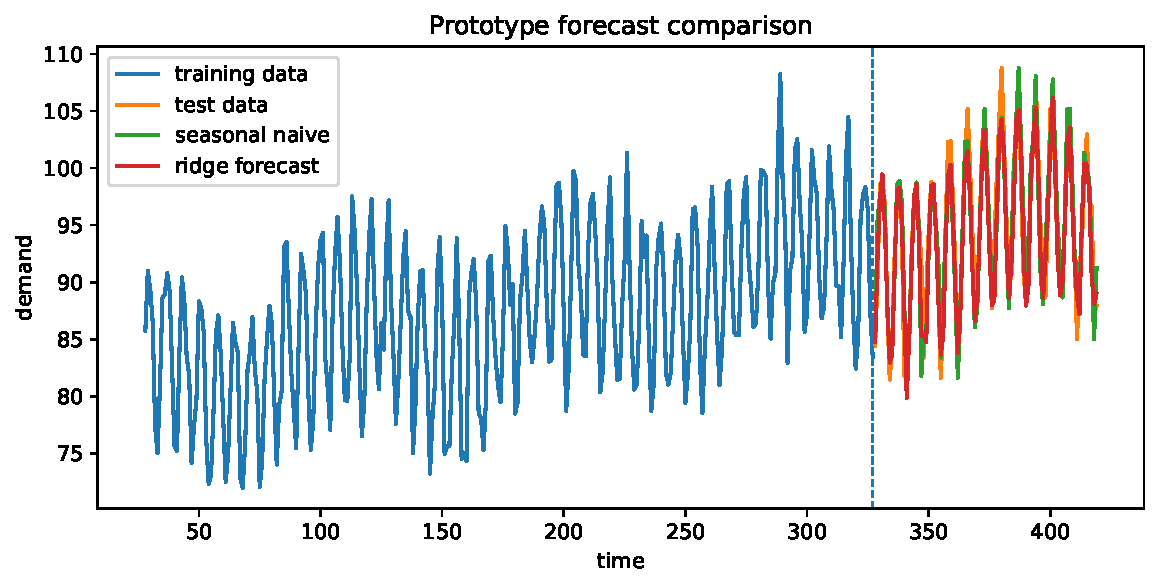
\includegraphics[keepaspectratio]{chapters/chapter-27-final-project-studio_files/figure-pdf/py-ch27-project-prototype-output-2.pdf}}

}

\caption{Prototype final-project workflow with baselines and a
lag-feature regression model.}

\end{figure}%

The example is intentionally modest. A final project should extend this
idea by adding rolling-origin validation, residual diagnostics,
uncertainty quantification, and a discussion of assumptions.

\section{27.9 Python example: rolling-origin
evaluation}\label{python-example-rolling-origin-evaluation}

The next example evaluates a one-step-ahead ridge model over many
forecast origins. The important point is that the model is refit at each
origin using only past information.

\begin{Shaded}
\begin{Highlighting}[]
\ImportTok{from}\NormalTok{ sklearn.base }\ImportTok{import}\NormalTok{ clone}

\NormalTok{origins }\OperatorTok{=}\NormalTok{ np.arange(}\DecValTok{220}\NormalTok{, }\BuiltInTok{len}\NormalTok{(df) }\OperatorTok{{-}} \DecValTok{1}\NormalTok{, }\DecValTok{7}\NormalTok{)}
\NormalTok{records }\OperatorTok{=}\NormalTok{ []}

\ControlFlowTok{for}\NormalTok{ origin }\KeywordTok{in}\NormalTok{ origins:}
\NormalTok{    train\_o }\OperatorTok{=}\NormalTok{ df.iloc[:origin].copy()}
\NormalTok{    test\_o }\OperatorTok{=}\NormalTok{ df.iloc[[origin]].copy()}

\NormalTok{    mdl }\OperatorTok{=}\NormalTok{ clone(model)}
\NormalTok{    mdl.fit(train\_o[feature\_cols], train\_o[}\StringTok{"y"}\NormalTok{])}

\NormalTok{    pred\_ridge }\OperatorTok{=} \BuiltInTok{float}\NormalTok{(mdl.predict(test\_o[feature\_cols])[}\DecValTok{0}\NormalTok{])}
\NormalTok{    pred\_naive }\OperatorTok{=} \BuiltInTok{float}\NormalTok{(test\_o[}\StringTok{"lag\_1"}\NormalTok{].iloc[}\DecValTok{0}\NormalTok{])}
\NormalTok{    pred\_seasonal }\OperatorTok{=} \BuiltInTok{float}\NormalTok{(test\_o[}\StringTok{"lag\_7"}\NormalTok{].iloc[}\DecValTok{0}\NormalTok{])}
\NormalTok{    actual }\OperatorTok{=} \BuiltInTok{float}\NormalTok{(test\_o[}\StringTok{"y"}\NormalTok{].iloc[}\DecValTok{0}\NormalTok{])}

\NormalTok{    records.extend([}
\NormalTok{        \{}\StringTok{"origin"}\NormalTok{: }\BuiltInTok{int}\NormalTok{(origin), }\StringTok{"model"}\NormalTok{: }\StringTok{"ridge"}\NormalTok{, }\StringTok{"error"}\NormalTok{: actual }\OperatorTok{{-}}\NormalTok{ pred\_ridge\},}
\NormalTok{        \{}\StringTok{"origin"}\NormalTok{: }\BuiltInTok{int}\NormalTok{(origin), }\StringTok{"model"}\NormalTok{: }\StringTok{"naive"}\NormalTok{, }\StringTok{"error"}\NormalTok{: actual }\OperatorTok{{-}}\NormalTok{ pred\_naive\},}
\NormalTok{        \{}\StringTok{"origin"}\NormalTok{: }\BuiltInTok{int}\NormalTok{(origin), }\StringTok{"model"}\NormalTok{: }\StringTok{"seasonal\_naive"}\NormalTok{, }\StringTok{"error"}\NormalTok{: actual }\OperatorTok{{-}}\NormalTok{ pred\_seasonal\},}
\NormalTok{    ])}

\NormalTok{err\_df }\OperatorTok{=}\NormalTok{ pd.DataFrame(records)}
\NormalTok{roll\_summary }\OperatorTok{=}\NormalTok{ (}
\NormalTok{    err\_df.assign(abs\_error}\OperatorTok{=}\KeywordTok{lambda}\NormalTok{ d: d[}\StringTok{"error"}\NormalTok{].}\BuiltInTok{abs}\NormalTok{())}
\NormalTok{    .groupby(}\StringTok{"model"}\NormalTok{, as\_index}\OperatorTok{=}\VariableTok{False}\NormalTok{)}
\NormalTok{    .agg(MAE}\OperatorTok{=}\NormalTok{(}\StringTok{"abs\_error"}\NormalTok{, }\StringTok{"mean"}\NormalTok{), Bias}\OperatorTok{=}\NormalTok{(}\StringTok{"error"}\NormalTok{, }\StringTok{"mean"}\NormalTok{))}
\NormalTok{)}
\BuiltInTok{print}\NormalTok{(roll\_summary.}\BuiltInTok{round}\NormalTok{(}\DecValTok{3}\NormalTok{))}

\NormalTok{plt.figure(figsize}\OperatorTok{=}\NormalTok{(}\DecValTok{8}\NormalTok{, }\DecValTok{4}\NormalTok{))}
\ControlFlowTok{for}\NormalTok{ name, g }\KeywordTok{in}\NormalTok{ err\_df.groupby(}\StringTok{"model"}\NormalTok{):}
\NormalTok{    plt.plot(g[}\StringTok{"origin"}\NormalTok{], g[}\StringTok{"error"}\NormalTok{], marker}\OperatorTok{=}\StringTok{"o"}\NormalTok{, linewidth}\OperatorTok{=}\DecValTok{1}\NormalTok{, label}\OperatorTok{=}\NormalTok{name)}
\NormalTok{plt.axhline(}\DecValTok{0}\NormalTok{, linewidth}\OperatorTok{=}\DecValTok{1}\NormalTok{)}
\NormalTok{plt.xlabel(}\StringTok{"forecast origin"}\NormalTok{)}
\NormalTok{plt.ylabel(}\StringTok{"forecast error"}\NormalTok{)}
\NormalTok{plt.title(}\StringTok{"Rolling{-}origin forecast errors"}\NormalTok{)}
\NormalTok{plt.legend()}
\NormalTok{plt.show()}
\end{Highlighting}
\end{Shaded}

\begin{verbatim}
            model    MAE   Bias
0           naive  4.789 -4.789
1           ridge  1.679  0.385
2  seasonal_naive  1.738  0.256
\end{verbatim}

\begin{figure}[H]

{\centering \pandocbounded{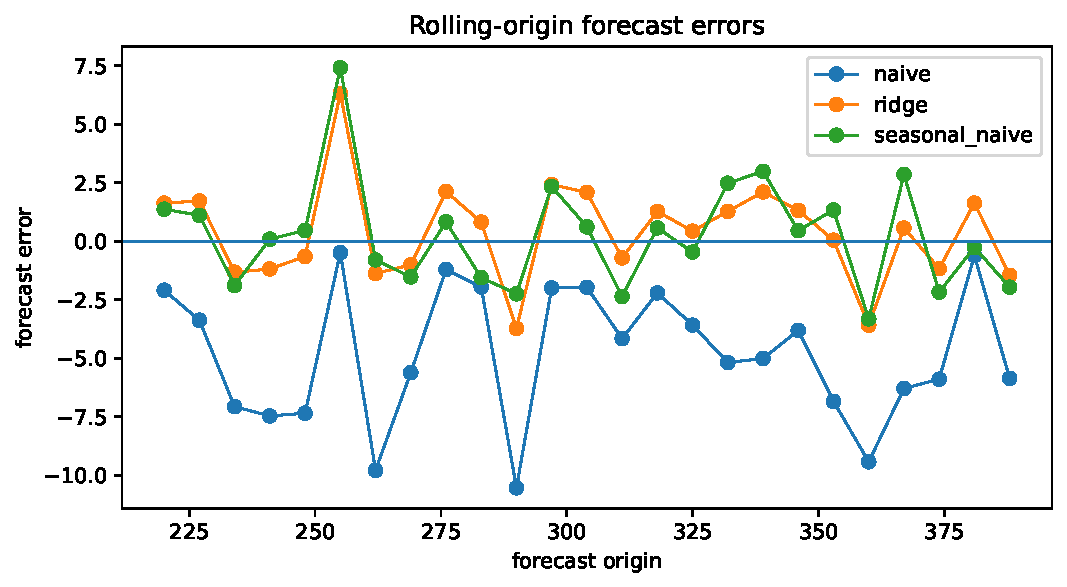
\includegraphics[keepaspectratio]{chapters/chapter-27-final-project-studio_files/figure-pdf/py-ch27-rolling-origin-output-2.pdf}}

}

\caption{Rolling-origin validation errors for a lag-feature forecasting
model.}

\end{figure}%

\section{27.10 Diagnostics and evidence}\label{diagnostics-and-evidence}

The project report should include evidence that the chosen model is
adequate for the task. The diagnostic evidence depends on the project
type.

For forecasting, include:

\begin{itemize}
\tightlist
\item
  time plot of actual values and forecasts;
\item
  horizon-wise error table;
\item
  residual ACF or error autocorrelation;
\item
  residual plot over time;
\item
  comparison against baselines;
\item
  prediction-interval coverage, if intervals are used.
\end{itemize}

For classification, include:

\begin{itemize}
\tightlist
\item
  train/validation/test split description;
\item
  confusion matrix;
\item
  precision, recall, F1, and calibration if probabilities are used;
\item
  an explanation of how overlapping windows are handled;
\item
  a baseline classifier.
\end{itemize}

For anomaly detection, include:

\begin{itemize}
\tightlist
\item
  anomaly-score time plot;
\item
  threshold selection rule;
\item
  false-positive/false-negative discussion if labels exist;
\item
  examples of detected anomalies;
\item
  sensitivity analysis for the threshold.
\end{itemize}

For spectral analysis, include:

\begin{itemize}
\tightlist
\item
  time plot;
\item
  periodogram or smoothed spectral estimate;
\item
  discussion of aliasing and sampling frequency;
\item
  comparison against time-domain evidence;
\item
  uncertainty or robustness checks.
\end{itemize}

\section{27.11 Interactive module: project rubric
dashboard}\label{interactive-module-project-rubric-dashboard}

This dashboard translates the final-project expectations into a
self-check score. It is designed for project planning, not for automatic
grading.

Interactive Module: Final Project Rubric Dashboard

Move the sliders to estimate the current state of your project draft.

Problem contract
\protect\phantomsection\label{ch27_rubric_contract_value}{3}
Mathematical theory
\protect\phantomsection\label{ch27_rubric_theory_value}{3} Validation
design \protect\phantomsection\label{ch27_rubric_validation_value}{3}
Baselines and comparison
\protect\phantomsection\label{ch27_rubric_baselines_value}{3}
Diagnostics and uncertainty
\protect\phantomsection\label{ch27_rubric_diagnostics_value}{3}
Reproducibility
\protect\phantomsection\label{ch27_rubric_repro_value}{3} Interactive
explanation
\protect\phantomsection\label{ch27_rubric_interactive_value}{3}
Communication \protect\phantomsection\label{ch27_rubric_comm_value}{3}

\protect\phantomsection\label{ch27_rubric_plot}

\section{27.12 AI-assisted project
workflow}\label{ai-assisted-project-workflow}

AI tools can help students plan, code, debug, and communicate. They
should not replace statistical reasoning. In this course, AI assistance
should be used as a \textbf{critic} and \textbf{co-pilot}, not as an
authority.

A useful AI-assisted workflow is:

\begin{enumerate}
\def\labelenumi{\arabic{enumi}.}
\tightlist
\item
  Write the project contract yourself.
\item
  Ask AI to identify possible leakage and invalid validation.
\item
  Ask AI to propose baseline methods.
\item
  Ask AI to review code for time-index mistakes.
\item
  Ask AI to critique residual diagnostics.
\item
  Ask AI to rewrite the report for clarity.
\item
  Verify every technical claim independently.
\end{enumerate}

\section{AI-assisted study box}\label{ai-assisted-study-box-4}

Use this prompt after you have a first draft:

\begin{quote}
I am writing a final project for a graduate course on modern time series
analysis and sequence learning. My task is {[}forecasting / anomaly
detection / classification / representation learning{]}. My target is
{[}\ldots{]}. My information set at the decision time is {[}\ldots{]}.
My validation design is {[}\ldots{]}. My baselines are {[}\ldots{]}. My
main model is {[}\ldots{]}. Please act as a skeptical reviewer. Identify
possible leakage, weak assumptions, missing diagnostics, unsupported
conclusions, and unclear mathematical definitions. For each issue,
suggest one concrete verification step.
\end{quote}

\section{27.13 Required final-project
deliverables}\label{required-final-project-deliverables}

Each final project should include the following deliverables.

\subsection{Written report}\label{written-report}

The written report should contain:

\begin{enumerate}
\def\labelenumi{\arabic{enumi}.}
\tightlist
\item
  title and abstract;
\item
  data description;
\item
  project contract;
\item
  mathematical formulation;
\item
  baseline methods;
\item
  main model or models;
\item
  validation design;
\item
  results and diagnostics;
\item
  uncertainty or limitations;
\item
  AI-assisted workflow note;
\item
  conclusion.
\end{enumerate}

\subsection{Reproducible notebook}\label{reproducible-notebook}

The notebook should run from top to bottom and produce the main results.
It should include:

\begin{itemize}
\tightlist
\item
  package imports;
\item
  data-loading or simulation section;
\item
  preprocessing section;
\item
  baseline models;
\item
  main model;
\item
  validation loop;
\item
  figures and tables;
\item
  diagnostic checks;
\item
  final summary.
\end{itemize}

\subsection{Interactive HTML
component}\label{interactive-html-component}

The interactive component can be simple. It should teach one important
idea from the project, such as:

\begin{itemize}
\tightlist
\item
  how a forecast horizon changes the training examples;
\item
  how a changepoint changes forecast behavior;
\item
  how an anomaly threshold changes false positives;
\item
  how an attention map changes across a sequence;
\item
  how rolling-origin validation differs from random splitting;
\item
  how a frequency peak appears in the periodogram.
\end{itemize}

\subsection{Short presentation}\label{short-presentation}

The presentation should explain:

\begin{enumerate}
\def\labelenumi{\arabic{enumi}.}
\tightlist
\item
  the problem;
\item
  the model;
\item
  the validation design;
\item
  the main result;
\item
  one limitation.
\end{enumerate}

\section{27.14 Suggested project topics}\label{suggested-project-topics}

\subsection{Forecasting topics}\label{forecasting-topics}

\begin{itemize}
\tightlist
\item
  electricity demand forecasting;
\item
  public transportation ridership;
\item
  financial volatility;
\item
  retail demand;
\item
  air quality or temperature forecasting;
\item
  web traffic or app usage;
\item
  academic enrollment or course demand.
\end{itemize}

\subsection{Sequence-learning topics}\label{sequence-learning-topics}

\begin{itemize}
\tightlist
\item
  sensor sequence classification;
\item
  ECG or biomedical signal classification;
\item
  anomaly detection in machine monitoring;
\item
  activity recognition;
\item
  sequence embeddings and clustering;
\item
  transformer-based sequence classification.
\end{itemize}

\subsection{Spectral and multiresolution
topics}\label{spectral-and-multiresolution-topics}

\begin{itemize}
\tightlist
\item
  detecting dominant frequencies in climate or signal data;
\item
  comparing Fourier and wavelet analysis;
\item
  filtering and denoising;
\item
  detecting transient bursts;
\item
  seasonal-frequency interpretation.
\end{itemize}

\subsection{AI-assisted modeling
topics}\label{ai-assisted-modeling-topics}

\begin{itemize}
\tightlist
\item
  compare human-designed and AI-suggested forecasting workflows;
\item
  audit AI-generated time-series code for leakage;
\item
  build an AI-assisted residual-diagnostics checklist;
\item
  evaluate whether AI can correctly identify ARIMA/SARIMA structure from
  plots.
\end{itemize}

\section{27.15 Common mistakes}\label{common-mistakes-26}

\begin{tcolorbox}[enhanced jigsaw, arc=.35mm, bottomrule=.15mm, bottomtitle=1mm, breakable, colback=white, colbacktitle=quarto-callout-warning-color!10!white, colframe=quarto-callout-warning-color-frame, coltitle=black, left=2mm, leftrule=.75mm, opacityback=0, opacitybacktitle=0.6, rightrule=.15mm, title=\textcolor{quarto-callout-warning-color}{\faExclamationTriangle}\hspace{0.5em}{Common mistakes}, titlerule=0mm, toprule=.15mm, toptitle=1mm]

\begin{enumerate}
\def\labelenumi{\arabic{enumi}.}
\tightlist
\item
  \textbf{Using random train-test splits for forecasting.} This usually
  leaks future structure.
\item
  \textbf{Skipping baselines.} A complex model that does not beat
  seasonal naive is not useful.
\item
  \textbf{Scaling on the full data set.} Fit scalers only on training
  data within each split.
\item
  \textbf{Using future covariates.} Only use variables known at the
  forecast origin.
\item
  \textbf{Reporting only one split.} A single lucky split can be
  misleading.
\item
  \textbf{Ignoring horizon-specific errors.} One-step performance may
  not reflect long-horizon behavior.
\item
  \textbf{Showing a model without diagnostics.} Validation error is not
  the whole story.
\item
  \textbf{Trusting AI-generated code without inspection.} AI code may
  accidentally use future observations.
\end{enumerate}

\end{tcolorbox}

\section{27.16 Exercises}\label{exercises-26}

\begin{enumerate}
\def\labelenumi{\arabic{enumi}.}
\tightlist
\item
  \textbf{Project contract.} Write a project contract for a
  one-week-ahead demand forecasting problem. Identify \(Y_t\),
  \(\mathcal F_t\), \(\mathcal H\), the loss function, and two
  baselines.
\item
  \textbf{Leakage audit.} Give three examples of leakage in a
  feature-based forecasting project. For each one, write a unit test or
  diagnostic check.
\item
  \textbf{Rolling-origin design.} Suppose \(n=1000\), initial training
  size is \(500\), horizon is \(H=20\), and origins are spaced every
  \(10\) observations. How many forecast origins are available?
\item
  \textbf{Baseline comparison.} Simulate a seasonal time series and
  compare naive, seasonal naive, and a lag-feature linear model.
\item
  \textbf{Interactive design.} Propose one interactive visualization for
  a final project on anomaly detection.
\item
  \textbf{AI critique.} Ask an AI assistant to critique your project
  design. Then write a paragraph explaining which suggestions you
  accepted, rejected, or verified.
\end{enumerate}

\section{27.17 Mini project}\label{mini-project-9}

Choose one of the following mini-project prompts and complete a two-page
report plus one notebook.

\subsection{Option A: Forecasting mini
project}\label{option-a-forecasting-mini-project}

Use a real or simulated time series. Compare at least three models:
naive, seasonal naive, and one learned model. Use rolling-origin
validation and report MAE/RMSE. Include one residual diagnostic and one
limitation.

\subsection{Option B: Anomaly detection mini
project}\label{option-b-anomaly-detection-mini-project}

Create or find a time series with anomalies. Build at least two anomaly
scores. Compare threshold behavior. Include an interactive threshold
explorer.

\subsection{Option C: Sequence classification mini
project}\label{option-c-sequence-classification-mini-project}

Use labeled sequences or simulated sequences. Compare summary-feature
logistic regression with a neural sequence model. Use a split that
avoids overlap leakage.

\subsection{Option D: AI-assisted modeling mini
project}\label{option-d-ai-assisted-modeling-mini-project}

Generate a time-series modeling plan with an AI assistant. Audit the
plan for leakage, missing baselines, invalid diagnostics, and unclear
assumptions. Implement a corrected version.

\section{27.18 Final checklist}\label{final-checklist}

Before submitting the final project, check the following.

\begin{itemize}
\tightlist
\item
  The problem is mathematically defined.
\item
  The information set \(\mathcal F_t\) is explicit.
\item
  The validation split respects time or sequence grouping.
\item
  At least one baseline is included.
\item
  The main model is justified by the data and task.
\item
  The report includes diagnostic plots or tables.
\item
  The notebook runs from top to bottom.
\item
  The interactive HTML component works without loading Plotly.js again.
\item
  The AI-assisted component is documented and verified.
\item
  The conclusion states limitations, not only successes.
\end{itemize}

\begin{tcolorbox}[enhanced jigsaw, arc=.35mm, bottomrule=.15mm, bottomtitle=1mm, breakable, colback=white, colbacktitle=quarto-callout-note-color!10!white, colframe=quarto-callout-note-color-frame, coltitle=black, left=2mm, leftrule=.75mm, opacityback=0, opacitybacktitle=0.6, rightrule=.15mm, title=\textcolor{quarto-callout-note-color}{\faInfo}\hspace{0.5em}{End of the book}, titlerule=0mm, toprule=.15mm, toptitle=1mm]

This final chapter turns the methods of the course into an independent
project. A successful project demonstrates mathematical formulation,
computational skill, diagnostic judgment, communication, and responsible
use of AI tools.

\end{tcolorbox}

\cleardoublepage
\phantomsection
\addcontentsline{toc}{part}{Appendices}
\appendix

\chapter{Python Labs Summary}\label{python-labs-summary}

\chapter*{Python Labs Summary}\label{python-labs-summary-1}
\addcontentsline{toc}{chapter}{Python Labs Summary}

\markboth{Python Labs Summary}{Python Labs Summary}

This page collects the companion Python labs for \textbf{Modern Time
Series Analysis and Sequence Learning}. Each lab is a Jupyter notebook
stored in the \texttt{labs/} folder of the book repository and can be
opened directly in Google Colab.

Repository: \url{https://github.com/wanghemath/Book-MachineLearning2sda}

\begin{tcolorbox}[enhanced jigsaw, arc=.35mm, bottomrule=.15mm, bottomtitle=1mm, breakable, colback=white, colbacktitle=quarto-callout-tip-color!10!white, colframe=quarto-callout-tip-color-frame, coltitle=black, left=2mm, leftrule=.75mm, opacityback=0, opacitybacktitle=0.6, rightrule=.15mm, title=\textcolor{quarto-callout-tip-color}{\faLightbulb}\hspace{0.5em}{How to use the labs}, titlerule=0mm, toprule=.15mm, toptitle=1mm]

Use the \textbf{Open in Colab} link when reading the online book. In
Colab, choose \textbf{File \(\to\) Save a copy in Drive} before editing.
For local work, clone the repository and open the notebooks from the
\texttt{labs/} folder.

\end{tcolorbox}

\section{Lab table}\label{lab-table}

{\def\LTcaptype{none} % do not increment counter
\begin{longtable}[]{@{}
  >{\raggedleft\arraybackslash}p{(\linewidth - 4\tabcolsep) * \real{0.4000}}
  >{\raggedright\arraybackslash}p{(\linewidth - 4\tabcolsep) * \real{0.3000}}
  >{\raggedright\arraybackslash}p{(\linewidth - 4\tabcolsep) * \real{0.3000}}@{}}
\toprule\noalign{}
\begin{minipage}[b]{\linewidth}\raggedleft
Chapter
\end{minipage} & \begin{minipage}[b]{\linewidth}\raggedright
Lab
\end{minipage} & \begin{minipage}[b]{\linewidth}\raggedright
Main focus
\end{minipage} \\
\midrule\noalign{}
\endhead
\bottomrule\noalign{}
\endlastfoot
1 & \href{labs/chapter-01-why-time-series-and-sequences-lab.ipynb}{Why
Time Series and Sequence Data Are
Different}\href{https://colab.research.google.com/github/wanghemath/Book-MachineLearning2sda/blob/main/labs/chapter-01-why-time-series-and-sequences-lab.ipynb}{Open
in Colab} & simulate white noise, random walks, trend, seasonality, and
windowed sequence data \\
2 &
\href{labs/chapter-02-exploratory-data-analysis-lab.ipynb}{Exploratory
Data Analysis for Time
Series}\href{https://colab.research.google.com/github/wanghemath/Book-MachineLearning2sda/blob/main/labs/chapter-02-exploratory-data-analysis-lab.ipynb}{Open
in Colab} & time plots, smoothing, detrending, differencing, ACF, and
seasonal diagnostics \\
3 &
\href{labs/chapter-03-stationarity-autocovariance-acf-lab.ipynb}{Stationarity,
Autocovariance, and
Autocorrelation}\href{https://colab.research.google.com/github/wanghemath/Book-MachineLearning2sda/blob/main/labs/chapter-03-stationarity-autocovariance-acf-lab.ipynb}{Open
in Colab} & strict/weak stationarity examples, sample autocovariance,
ACF, AR(1), MA(1), and random walk \\
4 & \href{labs/chapter-04-linear-processes-ar-ma-arma-lab.ipynb}{Linear
Processes, AR, MA, and ARMA
Models}\href{https://colab.research.google.com/github/wanghemath/Book-MachineLearning2sda/blob/main/labs/chapter-04-linear-processes-ar-ma-arma-lab.ipynb}{Open
in Colab} & simulate AR, MA, ARMA processes, root conditions, causality,
invertibility, and ACF/PACF behavior \\
5 &
\href{labs/chapter-05-difference-equations-dynamic-behavior-lab.ipynb}{Difference
Equations and Dynamic
Behavior}\href{https://colab.research.google.com/github/wanghemath/Book-MachineLearning2sda/blob/main/labs/chapter-05-difference-equations-dynamic-behavior-lab.ipynb}{Open
in Colab} & linear recurrences, characteristic roots, damping,
oscillation, and explosive dynamics \\
6 &
\href{labs/chapter-06-forecasting-best-linear-prediction-lab.ipynb}{Forecasting
Theory and Best Linear
Prediction}\href{https://colab.research.google.com/github/wanghemath/Book-MachineLearning2sda/blob/main/labs/chapter-06-forecasting-best-linear-prediction-lab.ipynb}{Open
in Colab} & best linear prediction, forecast variance, AR forecasts, and
multi-step forecasting \\
7 &
\href{labs/chapter-07-estimation-identification-diagnostics-lab.ipynb}{Estimation,
Identification, and
Diagnostics}\href{https://colab.research.google.com/github/wanghemath/Book-MachineLearning2sda/blob/main/labs/chapter-07-estimation-identification-diagnostics-lab.ipynb}{Open
in Colab} & Yule-Walker, likelihood, AIC/BIC, residual ACF, Ljung-Box,
and model criticism \\
8 & \href{labs/chapter-08-arima-differencing-lab.ipynb}{ARIMA Models and
Differencing}\href{https://colab.research.google.com/github/wanghemath/Book-MachineLearning2sda/blob/main/labs/chapter-08-arima-differencing-lab.ipynb}{Open
in Colab} & integrated processes, choosing differences, ARIMA fitting,
over-differencing, and forecast reconstruction \\
9 &
\href{labs/chapter-09-sarima-multiple-seasonality-lab.ipynb}{Seasonal
ARIMA and Multiple
Seasonality}\href{https://colab.research.google.com/github/wanghemath/Book-MachineLearning2sda/blob/main/labs/chapter-09-sarima-multiple-seasonality-lab.ipynb}{Open
in Colab} & seasonal differencing, SARIMA fitting, seasonal baselines,
and residual diagnostics \\
10 &
\href{labs/chapter-10-state-space-kalman-filtering-lab.ipynb}{State-Space
Models and Kalman
Filtering}\href{https://colab.research.google.com/github/wanghemath/Book-MachineLearning2sda/blob/main/labs/chapter-10-state-space-kalman-filtering-lab.ipynb}{Open
in Colab} & local-level models, Kalman prediction/update, missing data,
smoothing, and state forecasts \\
11 &
\href{labs/chapter-11-hidden-markov-regime-switching-lab.ipynb}{Hidden
Markov Models and Regime
Switching}\href{https://colab.research.google.com/github/wanghemath/Book-MachineLearning2sda/blob/main/labs/chapter-11-hidden-markov-regime-switching-lab.ipynb}{Open
in Colab} & forward probabilities, Viterbi decoding, Gaussian HMMs, and
regime-switching simulations \\
12 &
\href{labs/chapter-12-spectral-analysis-frequency-domain-lab.ipynb}{Spectral
Analysis and the Frequency
Domain}\href{https://colab.research.google.com/github/wanghemath/Book-MachineLearning2sda/blob/main/labs/chapter-12-spectral-analysis-frequency-domain-lab.ipynb}{Open
in Colab} & sinusoidal processes, aliasing, spectral density, and
spectra of AR/MA models \\
13 & \href{labs/chapter-13-dft-fft-periodogram-lab.ipynb}{Discrete
Fourier Transform, FFT, and
Periodogram}\href{https://colab.research.google.com/github/wanghemath/Book-MachineLearning2sda/blob/main/labs/chapter-13-dft-fft-periodogram-lab.ipynb}{Open
in Colab} & DFT basis, FFT, periodogram, leakage, tapering, and peak
detection \\
14 & \href{labs/chapter-14-filtering-wavelets-lab.ipynb}{Filtering and
Wavelet
Transform}\href{https://colab.research.google.com/github/wanghemath/Book-MachineLearning2sda/blob/main/labs/chapter-14-filtering-wavelets-lab.ipynb}{Open
in Colab} & linear filters, frequency response, differencing filters,
Haar wavelets, and denoising \\
15 &
\href{labs/chapter-15-forecast-evaluation-backtesting-lab.ipynb}{Forecast
Evaluation and
Backtesting}\href{https://colab.research.google.com/github/wanghemath/Book-MachineLearning2sda/blob/main/labs/chapter-15-forecast-evaluation-backtesting-lab.ipynb}{Open
in Colab} & rolling-origin validation, baseline comparisons,
horizon-wise metrics, intervals, and leakage checks \\
16 &
\href{labs/chapter-16-automated-forecasting-prophet-lab.ipynb}{Automated
Forecasting and Prophet-Type Additive
Models}\href{https://colab.research.google.com/github/wanghemath/Book-MachineLearning2sda/blob/main/labs/chapter-16-automated-forecasting-prophet-lab.ipynb}{Open
in Colab} & trend, changepoints, Fourier seasonality, holiday effects,
Prophet-style models, and tuning \\
17 &
\href{labs/chapter-17-feature-based-machine-learning-lab.ipynb}{Feature-Based
Machine Learning for Time
Series}\href{https://colab.research.google.com/github/wanghemath/Book-MachineLearning2sda/blob/main/labs/chapter-17-feature-based-machine-learning-lab.ipynb}{Open
in Colab} & lag features, rolling features, calendar variables, Fourier
features, tree models, and validation \\
18 &
\href{labs/chapter-18-probabilistic-forecasting-uncertainty-lab.ipynb}{Probabilistic
Forecasting and Uncertainty
Quantification}\href{https://colab.research.google.com/github/wanghemath/Book-MachineLearning2sda/blob/main/labs/chapter-18-probabilistic-forecasting-uncertainty-lab.ipynb}{Open
in Colab} & prediction intervals, quantile loss, conformal prediction,
calibration, and risk decisions \\
19 &
\href{labs/chapter-19-neural-networks-for-time-series-lab.ipynb}{Neural
Networks for Time
Series}\href{https://colab.research.google.com/github/wanghemath/Book-MachineLearning2sda/blob/main/labs/chapter-19-neural-networks-for-time-series-lab.ipynb}{Open
in Colab} & sliding windows, scaling, MLP forecasting, PyTorch training,
and chronological validation \\
20 &
\href{labs/chapter-20-convolutional-models-sequences-lab.ipynb}{Convolutional
Models for
Sequences}\href{https://colab.research.google.com/github/wanghemath/Book-MachineLearning2sda/blob/main/labs/chapter-20-convolutional-models-sequences-lab.ipynb}{Open
in Colab} & causal convolution, dilation, receptive fields, TCNs, and
PyTorch Conv1d \\
21 & \href{labs/chapter-21-rnn-lstm-gru-lab.ipynb}{Recurrent Neural
Networks, LSTM, and
GRU}\href{https://colab.research.google.com/github/wanghemath/Book-MachineLearning2sda/blob/main/labs/chapter-21-rnn-lstm-gru-lab.ipynb}{Open
in Colab} & RNN hidden states, LSTM/GRU gates, sequence-to-one
forecasting, and recurrent training \\
22 &
\href{labs/chapter-22-attention-transformers-time-series-lab.ipynb}{Attention
and Transformer Models for Time
Series}\href{https://colab.research.google.com/github/wanghemath/Book-MachineLearning2sda/blob/main/labs/chapter-22-attention-transformers-time-series-lab.ipynb}{Open
in Colab} & scaled dot-product attention, causal masks, positional
encodings, and transformer forecasting \\
23 &
\href{labs/chapter-23-representation-learning-time-series-lab.ipynb}{Representation
Learning for Time
Series}\href{https://colab.research.google.com/github/wanghemath/Book-MachineLearning2sda/blob/main/labs/chapter-23-representation-learning-time-series-lab.ipynb}{Open
in Colab} & embeddings, PCA, autoencoders, masked reconstruction,
contrastive ideas, and anomaly detection \\
24 &
\href{labs/chapter-24-multivariate-panel-hierarchical-lab.ipynb}{Multivariate,
Panel, and Hierarchical Time
Series}\href{https://colab.research.google.com/github/wanghemath/Book-MachineLearning2sda/blob/main/labs/chapter-24-multivariate-panel-hierarchical-lab.ipynb}{Open
in Colab} & VAR models, coupling, Granger-style prediction, global
models, and reconciliation \\
25 &
\href{labs/chapter-25-ai-assisted-time-series-modeling-lab.ipynb}{AI-Assisted
Time-Series
Modeling}\href{https://colab.research.google.com/github/wanghemath/Book-MachineLearning2sda/blob/main/labs/chapter-25-ai-assisted-time-series-modeling-lab.ipynb}{Open
in Colab} & AI workflow auditing, prompt design, leakage review, code
review, and report checking \\
26 &
\href{labs/chapter-26-end-to-end-forecasting-pipeline-lab.ipynb}{End-to-End
Forecasting
Pipeline}\href{https://colab.research.google.com/github/wanghemath/Book-MachineLearning2sda/blob/main/labs/chapter-26-end-to-end-forecasting-pipeline-lab.ipynb}{Open
in Colab} & forecasting contracts, preprocessing, baselines, validation,
intervals, and monitoring \\
27 & \href{labs/chapter-27-final-project-studio-lab.ipynb}{Final Project
Studio}\href{https://colab.research.google.com/github/wanghemath/Book-MachineLearning2sda/blob/main/labs/chapter-27-final-project-studio-lab.ipynb}{Open
in Colab} & project design, validation planning, baselines, diagnostics,
rubric alignment, and final reporting \\
\end{longtable}
}

\section{Lab design pattern}\label{lab-design-pattern}

Most labs follow a common workflow:

\begin{enumerate}
\def\labelenumi{\arabic{enumi}.}
\tightlist
\item
  State the modeling question and identify the forecasting information
  set.
\item
  Simulate or load a time-series/sequence dataset.
\item
  Visualize the series, dependence structure, and diagnostics.
\item
  Fit at least one baseline model before fitting a more advanced model.
\item
  Evaluate with chronological or rolling-origin validation.
\item
  Interpret residuals, uncertainty, and failure modes.
\item
  Use AI assistance only after defining the mathematical task and then
  verify the output manually.
\end{enumerate}

\section{Recommended local setup}\label{recommended-local-setup}

\begin{Shaded}
\begin{Highlighting}[]
\FunctionTok{git}\NormalTok{ clone https://github.com/wanghemath/Book{-}MachineLearning2sda.git}
\BuiltInTok{cd}\NormalTok{ Book{-}MachineLearning2sda}
\ExtensionTok{python} \AttributeTok{{-}m}\NormalTok{ venv .venv}
\BuiltInTok{source}\NormalTok{ .venv/bin/activate  }\CommentTok{\# Windows: .venv\textbackslash{}Scripts\textbackslash{}activate}
\ExtensionTok{pip}\NormalTok{ install }\AttributeTok{{-}r}\NormalTok{ requirements.txt}
\ExtensionTok{jupyter}\NormalTok{ lab}
\end{Highlighting}
\end{Shaded}

Alternatively, use Conda:

\begin{Shaded}
\begin{Highlighting}[]
\ExtensionTok{conda}\NormalTok{ env create }\AttributeTok{{-}f}\NormalTok{ environment.yml}
\ExtensionTok{conda}\NormalTok{ activate ts{-}sequence{-}learning}
\ExtensionTok{jupyter}\NormalTok{ lab}
\end{Highlighting}
\end{Shaded}

\section{Responsible AI checklist for
labs}\label{responsible-ai-checklist-for-labs}

Before submitting any lab, verify the following.

\begin{itemize}
\tightlist
\item
  The train/validation/test split respects time order.
\item
  Scaling, imputation, feature engineering, and model selection use only
  information available at the forecast origin.
\item
  Every advanced model is compared with a baseline such as naive,
  seasonal naive, linear AR, ARIMA, or a simple feature model.
\item
  Residuals or forecast errors are examined, not only point metrics.
\item
  AI-generated code or explanations are checked against the mathematics
  and the data-generating process.
\item
  The final notebook is reproducible from a clean runtime.
\end{itemize}

\chapter{Interactive HTML Modules}\label{interactive-html-modules-1}

Browser-Based Visual Experiments for Modern Time Series Analysis and
Sequence Learning

\hfill\break

\chapter{Interactive HTML Modules}\label{interactive-html-modules-2}

This page collects the interactive browser modules used throughout
\emph{Modern Time Series Analysis and Sequence Learning}. The modules
are designed to help students move between four views of a model:

\begin{enumerate}
\def\labelenumi{\arabic{enumi}.}
\tightlist
\item
  the mathematical definition,
\item
  the simulated data,
\item
  the diagnostic plot,
\item
  the modeling interpretation.
\end{enumerate}

The interactive examples are ordinary HTML and JavaScript components
embedded in the Quarto chapters. They do not require a Python kernel, so
students can use them directly in the published website.

\section{Global Plotly setup}\label{global-plotly-setup}

The book loads Plotly.js once globally through
\texttt{assets/header.html}. Individual chapter files should not include
a second Plotly script tag.

The shared header has two jobs:

\begin{enumerate}
\def\labelenumi{\arabic{enumi}.}
\tightlist
\item
  load Plotly.js once;
\item
  load \texttt{assets/ts-interactives.js} using a path that works both
  from the book root and from pages inside \texttt{chapters/}.
\end{enumerate}

The interactive graphics use the shared Plotly configuration

\begin{Shaded}
\begin{Highlighting}[]
\BuiltInTok{window}\OperatorTok{.}\AttributeTok{TSInteractives}\OperatorTok{.}\AttributeTok{plotlyConfig} \OperatorTok{=}\NormalTok{ \{}
  \DataTypeTok{responsive}\OperatorTok{:} \KeywordTok{true}\OperatorTok{,}
  \DataTypeTok{displayModeBar}\OperatorTok{:} \KeywordTok{true}\OperatorTok{,}
  \DataTypeTok{displaylogo}\OperatorTok{:} \KeywordTok{false}\OperatorTok{,}
  \DataTypeTok{scrollZoom}\OperatorTok{:} \KeywordTok{true}\OperatorTok{,}
  \DataTypeTok{toImageButtonOptions}\OperatorTok{:}\NormalTok{ \{}
    \DataTypeTok{format}\OperatorTok{:} \StringTok{"png"}\OperatorTok{,}
    \DataTypeTok{filename}\OperatorTok{:} \StringTok{"time{-}series{-}interactive"}\OperatorTok{,}
    \DataTypeTok{height}\OperatorTok{:} \DecValTok{600}\OperatorTok{,}
    \DataTypeTok{width}\OperatorTok{:} \DecValTok{900}\OperatorTok{,}
    \DataTypeTok{scale}\OperatorTok{:} \DecValTok{2}
\NormalTok{  \}}
\NormalTok{\}}\OperatorTok{;}
\end{Highlighting}
\end{Shaded}

This enables the Plotly toolbar functions, including image download,
zoom, pan, box select, lasso select, zoom in, zoom out, autoscale, and
reset axes.

\section{Student guide}\label{student-guide}

Students should use each interactive module in three passes.

First, move one slider at a time and describe what changes in the plot.
Second, connect the observed change to a mathematical quantity such as
an ACF value, a root modulus, a forecast horizon, a receptive field, or
an attention weight. Third, write a modeling conclusion: what would this
visual evidence suggest in a real data analysis?

A good interactive answer should not only say what the plot shows. It
should also identify the model assumption being tested.

\section{Instructor guide}\label{instructor-guide}

The interactive modules are best used as short in-class experiments. A
useful pattern is:

\begin{enumerate}
\def\labelenumi{\arabic{enumi}.}
\tightlist
\item
  ask students to predict what will happen before moving the slider;
\item
  run the interactive module;
\item
  connect the visual output to the theorem or definition;
\item
  ask students to reproduce the same idea in the Python lab.
\end{enumerate}

The modules are also useful for AI-assisted learning. Students can ask
an AI assistant to explain the pattern, but they should verify the
explanation by citing the relevant equation or diagnostic rule from the
chapter.

\section{Module inventory}\label{module-inventory}

The following table gives the current interactive map for the e-book.

{\def\LTcaptype{none} % do not increment counter
\begin{longtable}[]{@{}
  >{\raggedleft\arraybackslash}p{(\linewidth - 6\tabcolsep) * \real{0.3077}}
  >{\raggedright\arraybackslash}p{(\linewidth - 6\tabcolsep) * \real{0.2308}}
  >{\raggedright\arraybackslash}p{(\linewidth - 6\tabcolsep) * \real{0.2308}}
  >{\raggedright\arraybackslash}p{(\linewidth - 6\tabcolsep) * \real{0.2308}}@{}}
\toprule\noalign{}
\begin{minipage}[b]{\linewidth}\raggedleft
Chapter
\end{minipage} & \begin{minipage}[b]{\linewidth}\raggedright
Interactive module
\end{minipage} & \begin{minipage}[b]{\linewidth}\raggedright
Main mathematical idea
\end{minipage} & \begin{minipage}[b]{\linewidth}\raggedright
Student task
\end{minipage} \\
\midrule\noalign{}
\endhead
\bottomrule\noalign{}
\endlastfoot
1 & Time-series process simulator & Stochastic processes, realizations,
dependence, ACF & Compare white noise, random walk, AR(1), MA(1), and
seasonal signals. \\
2 & EDA playground & Trend, seasonality, smoothing, differencing &
Decide whether detrending, differencing, or smoothing is appropriate. \\
3 & Stationarity and ACF playground & Weak stationarity, sample ACF,
theoretical ACF & Compare sample ACF with the theoretical pattern for AR
and MA processes. \\
4 & ARMA root and impulse-response explorer & AR roots, causality,
stationarity, impulse response & Move roots across the unit circle and
explain the resulting dynamics. \\
5 & Difference-equation dynamics explorer & Recurrence roots, damping,
oscillation, explosion & Interpret real and complex roots from the shape
of a recurrence. \\
6 & AR(1) forecast cone and BLP weights & Best linear prediction,
forecast variance, orthogonality & Explain how uncertainty grows as
forecast horizon increases. \\
7 & Model-identification and residual-diagnostics lab & ACF/PACF
identification, residual whiteness, Ljung--Box logic & Choose among
candidate ARMA models and justify the choice. \\
8 & Differencing explorer & Integrated processes, first and second
differences, over-differencing & Choose a differencing order and check
the ACF after differencing. \\
9 & Seasonal differencing and SARIMA explorer & Seasonal lag operators,
seasonal ACF, SARIMA structure & Identify seasonal dependence and
compare ordinary vs seasonal differencing. \\
10 & Kalman filter playground & State prediction, update, filtering,
observation noise & Observe how process noise and measurement noise
change the filtered state. \\
11 & Hidden-regime simulator & HMM states, transition probabilities,
emissions, decoding & Relate hidden states to observed regimes and
uncertainty. \\
12 & Spectral explorer & Frequency, period, aliasing, spectral power &
Detect hidden sinusoidal components in a noisy time series. \\
13 & DFT and periodogram explorer & Fourier basis, FFT, periodogram,
spectral leakage & Identify dominant Fourier frequencies and explain
resolution limits. \\
14 & Filtering and wavelet explorers & Linear filters, frequency
response, Haar details, denoising & Compare smoothing, differencing, and
wavelet thresholding. \\
15 & Rolling-origin backtesting simulator & Forecast horizon,
chronological validation, metrics & Compare forecast errors across
horizons and validation windows. \\
16 & Prophet-type additive model builder & Trend, changepoints, Fourier
seasonality, holidays & Decompose a forecast into trend, seasonal,
holiday, and noise components. \\
17 & Supervised feature matrix builder & Lag features, rolling windows,
horizon labels, leakage & Convert a time series into a
supervised-learning design matrix. \\
18 & Calibration and interval-width explorer & Probabilistic
forecasting, coverage, sharpness & Study the tradeoff between interval
width and empirical coverage. \\
19 & Neural-network window builder and activation explorer & Input
windows, label windows, nonlinear activations & Build valid training
windows and understand nonlinear transformations. \\
20 & Causal dilated convolution and TCN receptive field & 1D
convolution, causality, dilation, receptive field & Determine which past
observations influence a forecast. \\
21 & RNN hidden-state and gate explorer & Hidden states, memory,
LSTM/GRU gates & Compare short memory, long memory, and gated memory
behavior. \\
22 & Causal attention heatmap and positional encoding & Scaled
dot-product attention, causal mask, position information & Interpret
attention weights without using future information. \\
23 & Embedding and bottleneck reconstruction explorer & Representation
learning, autoencoders, anomaly scores & Examine how windows become
low-dimensional features. \\
24 & VAR coupling and reconciliation explorers & Multivariate
dependence, impulse response, hierarchical consistency & Analyze
cross-series coupling and reconcile aggregate forecasts. \\
25 & AI workflow auditor and prompt builder & Information sets, leakage
checks, AI-assisted critique & Audit a forecasting workflow and build a
responsible prompt. \\
26 & Forecasting pipeline and monitoring dashboard & End-to-end
pipeline, deployment drift, monitoring & Diagnose leakage, model choice,
and post-deployment error drift. \\
27 & Project design, rolling-origin planner, and rubric dashboard &
Project contract, validation plan, reproducibility & Plan a final
project and evaluate readiness using the rubric. \\
\end{longtable}
}

\section{Chapter links}\label{chapter-links}

Use the links below to go directly to the chapters that contain the
interactive modules.

{\def\LTcaptype{none} % do not increment counter
\begin{longtable}[]{@{}
  >{\raggedleft\arraybackslash}p{(\linewidth - 2\tabcolsep) * \real{0.5714}}
  >{\raggedright\arraybackslash}p{(\linewidth - 2\tabcolsep) * \real{0.4286}}@{}}
\toprule\noalign{}
\begin{minipage}[b]{\linewidth}\raggedleft
Chapter
\end{minipage} & \begin{minipage}[b]{\linewidth}\raggedright
Link
\end{minipage} \\
\midrule\noalign{}
\endhead
\bottomrule\noalign{}
\endlastfoot
1 & \hyperref[why-time-series-and-sequence-data-are-different]{Why Time
Series and Sequences?} \\
2 & \hyperref[exploratory-data-analysis-for-time-series]{Exploratory
Data Analysis} \\
3 &
\hyperref[stationarity-autocovariance-and-autocorrelation]{Stationarity,
Autocovariance, and ACF} \\
4 & \hyperref[linear-processes-ar-ma-and-arma-models]{Linear Processes,
AR, MA, and ARMA} \\
5 & \hyperref[difference-equations-and-dynamic-behavior]{Difference
Equations and Dynamic Behavior} \\
6 & \hyperref[forecasting-theory-and-best-linear-prediction]{Forecasting
and Best Linear Prediction} \\
7 &
\hyperref[estimation-model-identification-and-diagnostics]{Estimation,
Identification, and Diagnostics} \\
8 & \hyperref[arima-models-and-differencing]{ARIMA and Differencing} \\
9 & \hyperref[seasonal-arima-and-multiple-seasonality]{SARIMA and
Multiple Seasonality} \\
10 & \hyperref[state-space-models-and-kalman-filtering]{State-Space
Models and Kalman Filtering} \\
11 & \hyperref[hidden-markov-models-and-regime-switching]{Hidden Markov
Models and Regime Switching} \\
12 & \hyperref[spectral-analysis-and-the-frequency-domain]{Spectral
Analysis and the Frequency Domain} \\
13 & \hyperref[discrete-fourier-transform-fft-and-the-periodogram]{DFT,
FFT, and Periodogram} \\
14 & \hyperref[filtering-and-wavelet-transform]{Filtering and
Wavelets} \\
15 & \hyperref[forecast-evaluation-and-backtesting]{Forecast Evaluation
and Backtesting} \\
16 &
\hyperref[automated-forecasting-and-prophet-type-additive-models]{Automated
Forecasting and Prophet-Type Models} \\
17 &
\hyperref[feature-based-machine-learning-for-time-series]{Feature-Based
Machine Learning} \\
18 &
\hyperref[probabilistic-forecasting-and-uncertainty-quantification]{Probabilistic
Forecasting and Uncertainty} \\
19 & \hyperref[neural-networks-for-time-series]{Neural Networks for Time
Series} \\
20 & \hyperref[convolutional-models-for-sequences]{Convolutional Models
for Sequences} \\
21 & \hyperref[recurrent-neural-networks-lstm-and-gru]{RNN, LSTM, and
GRU} \\
22 &
\hyperref[attention-and-transformer-models-for-time-series-and-sequence-data]{Attention
and Transformers for Time Series} \\
23 & \hyperref[representation-learning-for-time-series]{Representation
Learning for Time Series} \\
24 &
\hyperref[multivariate-panel-and-hierarchical-time-series]{Multivariate,
Panel, and Hierarchical Time Series} \\
25 & \hyperref[ai-assisted-time-series-modeling]{AI-Assisted Time-Series
Modeling} \\
26 & \hyperref[end-to-end-forecasting-pipeline]{End-to-End Forecasting
Pipeline} \\
27 & \hyperref[final-project-studio]{Final Project Studio} \\
\end{longtable}
}

\section{Common controls}\label{common-controls}

Most modules use one or more of the following controls.

{\def\LTcaptype{none} % do not increment counter
\begin{longtable}[]{@{}
  >{\raggedright\arraybackslash}p{(\linewidth - 4\tabcolsep) * \real{0.3333}}
  >{\raggedright\arraybackslash}p{(\linewidth - 4\tabcolsep) * \real{0.3333}}
  >{\raggedright\arraybackslash}p{(\linewidth - 4\tabcolsep) * \real{0.3333}}@{}}
\toprule\noalign{}
\begin{minipage}[b]{\linewidth}\raggedright
Control type
\end{minipage} & \begin{minipage}[b]{\linewidth}\raggedright
Meaning in the book
\end{minipage} & \begin{minipage}[b]{\linewidth}\raggedright
Example interpretation
\end{minipage} \\
\midrule\noalign{}
\endhead
\bottomrule\noalign{}
\endlastfoot
Model selector & Chooses the data-generating process or model family &
White noise, random walk, AR(1), MA(1), SARIMA, neural model. \\
Parameter slider & Changes one numerical model parameter & AR
coefficient, MA coefficient, root radius, dilation, horizon. \\
Window slider & Chooses a training window or forecast origin & Shows
which observations are inputs and which are labels. \\
Noise slider & Changes observation noise or innovation variance & Helps
distinguish signal structure from random variation. \\
Horizon slider & Changes how far ahead the model forecasts & Shows
increasing uncertainty and horizon-specific error. \\
Diagnostic plot & Displays evidence about model adequacy & ACF,
periodogram, residual error, calibration, attention heatmap. \\
\end{longtable}
}

\section{Plotly toolbar functions}\label{plotly-toolbar-functions}

Every Plotly module is configured to show the modebar. The most useful
buttons for students are:

{\def\LTcaptype{none} % do not increment counter
\begin{longtable}[]{@{}
  >{\raggedright\arraybackslash}p{(\linewidth - 2\tabcolsep) * \real{0.5000}}
  >{\raggedright\arraybackslash}p{(\linewidth - 2\tabcolsep) * \real{0.5000}}@{}}
\toprule\noalign{}
\begin{minipage}[b]{\linewidth}\raggedright
Button
\end{minipage} & \begin{minipage}[b]{\linewidth}\raggedright
Use
\end{minipage} \\
\midrule\noalign{}
\endhead
\bottomrule\noalign{}
\endlastfoot
Download PNG & Save a figure for notes, homework, or project reports. \\
Zoom & Inspect local structure, spikes, or high-error periods. \\
Pan & Move across a long time axis. \\
Autoscale & Return to a good automatic view after zooming. \\
Reset axes & Return to the original plot view. \\
Box select / lasso select & Explore local regions in scatter, embedding,
and diagnostic plots. \\
\end{longtable}
}

\section{Implementation pattern}\label{implementation-pattern}

A chapter-level interactive module should contain only the HTML
container and the module-specific script. It should not load Plotly.js
again.

A safe pattern is:

\begin{Shaded}
\begin{Highlighting}[]
\DataTypeTok{\textless{}}\KeywordTok{div}\OtherTok{ class}\OperatorTok{=}\StringTok{"interactive{-}card"}\DataTypeTok{\textgreater{}}
  \DataTypeTok{\textless{}}\KeywordTok{h3}\DataTypeTok{\textgreater{}}\NormalTok{Interactive module title}\DataTypeTok{\textless{}/}\KeywordTok{h3}\DataTypeTok{\textgreater{}}
  \DataTypeTok{\textless{}}\KeywordTok{label}\DataTypeTok{\textgreater{}}
\NormalTok{    Parameter:}
    \DataTypeTok{\textless{}}\KeywordTok{input}\OtherTok{ id}\OperatorTok{=}\StringTok{"example{-}slider"}\OtherTok{ type}\OperatorTok{=}\StringTok{"range"}\OtherTok{ min}\OperatorTok{=}\StringTok{"0"}\OtherTok{ max}\OperatorTok{=}\StringTok{"1"}\OtherTok{ step}\OperatorTok{=}\StringTok{"0.01"}\OtherTok{ value}\OperatorTok{=}\StringTok{"0.5"}\DataTypeTok{\textgreater{}}
  \DataTypeTok{\textless{}/}\KeywordTok{label}\DataTypeTok{\textgreater{}}
  \DataTypeTok{\textless{}}\KeywordTok{span}\OtherTok{ id}\OperatorTok{=}\StringTok{"example{-}slider{-}value"}\DataTypeTok{\textgreater{}\textless{}/}\KeywordTok{span}\DataTypeTok{\textgreater{}}
  \DataTypeTok{\textless{}}\KeywordTok{div}\OtherTok{ id}\OperatorTok{=}\StringTok{"example{-}plot"}\OtherTok{ style}\OperatorTok{=}\StringTok{"height:420px;"}\DataTypeTok{\textgreater{}\textless{}/}\KeywordTok{div}\DataTypeTok{\textgreater{}}
\DataTypeTok{\textless{}/}\KeywordTok{div}\DataTypeTok{\textgreater{}}
\end{Highlighting}
\end{Shaded}

Then the JavaScript should call Plotly using the shared configuration:

\begin{Shaded}
\begin{Highlighting}[]
\NormalTok{Plotly}\OperatorTok{.}\FunctionTok{newPlot}\NormalTok{(}
  \StringTok{"example{-}plot"}\OperatorTok{,}
\NormalTok{  traces}\OperatorTok{,}
\NormalTok{  layout}\OperatorTok{,}
  \BuiltInTok{window}\OperatorTok{.}\AttributeTok{TSInteractives}\OperatorTok{.}\AttributeTok{plotlyConfig}
\NormalTok{)}\OperatorTok{;}
\end{Highlighting}
\end{Shaded}

For modules that update repeatedly, use \texttt{Plotly.react}:

\begin{Shaded}
\begin{Highlighting}[]
\NormalTok{Plotly}\OperatorTok{.}\FunctionTok{react}\NormalTok{(}
  \StringTok{"example{-}plot"}\OperatorTok{,}
\NormalTok{  traces}\OperatorTok{,}
\NormalTok{  layout}\OperatorTok{,}
  \BuiltInTok{window}\OperatorTok{.}\AttributeTok{TSInteractives}\OperatorTok{.}\AttributeTok{plotlyConfig}
\NormalTok{)}\OperatorTok{;}
\end{Highlighting}
\end{Shaded}

\section{Quality checks for new
modules}\label{quality-checks-for-new-modules}

Before adding a new interactive example, check the following.

\begin{enumerate}
\def\labelenumi{\arabic{enumi}.}
\tightlist
\item
  The chapter does not include another external Plotly.js script tag.
\item
  The HTML ids are unique across the book.
\item
  The sliders update their displayed numerical values.
\item
  The graph appears on both local preview and GitHub Pages.
\item
  The module works from a page inside \texttt{chapters/}.
\item
  The module does not rely on a Python kernel.
\item
  The mathematical interpretation is stated next to the plot.
\item
  The module is usable in class, homework, and self-study.
\item
  The module is connected to a Python lab exercise.
\item
  The module does not create a raw HTML table that can interfere with
  PDF rendering.
\end{enumerate}

\section{AI-assisted learning
prompts}\label{ai-assisted-learning-prompts}

Students may use the following prompts after experimenting with an
interactive module.

\textbf{Prompt 1. Explain the visual change.}

\begin{Shaded}
\begin{Highlighting}[]
\NormalTok{I changed the parameter from \_\_\_ to \_\_\_. The plot changed in the following way: \_\_\_. Explain this change using the mathematical model, not only visual intuition.}
\end{Highlighting}
\end{Shaded}

\textbf{Prompt 2. Connect the interactive plot to diagnostics.}

\begin{Shaded}
\begin{Highlighting}[]
\NormalTok{Given this time{-}series plot and diagnostic plot, what model assumption is being checked? What evidence would support or reject the assumption?}
\end{Highlighting}
\end{Shaded}

\textbf{Prompt 3. Check for leakage.}

\begin{Shaded}
\begin{Highlighting}[]
\NormalTok{In this forecasting setup, identify the forecast origin, the information set, the target horizon, and any variables that may leak future information.}
\end{Highlighting}
\end{Shaded}

\textbf{Prompt 4. Turn the interactive idea into Python.}

\begin{Shaded}
\begin{Highlighting}[]
\NormalTok{Write Python code that reproduces the idea in this interactive module using NumPy, pandas, matplotlib, and statsmodels or PyTorch where appropriate. Explain how to validate the result.}
\end{Highlighting}
\end{Shaded}

\section{Development notes}\label{development-notes}

The interactive system uses two complementary approaches.

First, the shared file \texttt{assets/ts-interactives.js} contains
reusable utilities, shared Plotly configuration, and several
chapter-specific initialization functions. Second, some chapters include
local inline scripts for modules that are easier to keep next to the
mathematical explanation.

Both approaches are acceptable, provided that Plotly.js itself is loaded
only once globally from \texttt{assets/header.html}.

\section{Troubleshooting}\label{troubleshooting}

{\def\LTcaptype{none} % do not increment counter
\begin{longtable}[]{@{}
  >{\raggedright\arraybackslash}p{(\linewidth - 4\tabcolsep) * \real{0.3333}}
  >{\raggedright\arraybackslash}p{(\linewidth - 4\tabcolsep) * \real{0.3333}}
  >{\raggedright\arraybackslash}p{(\linewidth - 4\tabcolsep) * \real{0.3333}}@{}}
\toprule\noalign{}
\begin{minipage}[b]{\linewidth}\raggedright
Problem
\end{minipage} & \begin{minipage}[b]{\linewidth}\raggedright
Likely cause
\end{minipage} & \begin{minipage}[b]{\linewidth}\raggedright
Fix
\end{minipage} \\
\midrule\noalign{}
\endhead
\bottomrule\noalign{}
\endlastfoot
The plot area is blank. & Plotly was not loaded or the script path is
wrong. & Check \texttt{assets/header.html} and browser console. \\
Browser reports \texttt{chapters/assets/ts-interactives.js} not found. &
The script path is relative to the chapter folder. & Use the dynamic
path logic in \texttt{assets/header.html}. \\
Sliders move but the plot does not update. & The JavaScript listener is
not attached or an id does not match. & Check that the slider id in HTML
matches the id in JavaScript. \\
The PDF build warns about raw HTML tables. & An interactive module
created a literal HTML table. & Replace it with text, markdown, or a
Plotly/table-free summary. \\
A module works locally but not on GitHub Pages. & File path or
case-sensitivity issue. & Check exact filenames and folder names. \\
The toolbar covers the title. & Top plot margin is too small. & Increase
\texttt{layout.margin.t} or use a shorter title. \\
\end{longtable}
}

\section{Recommended extension plan}\label{recommended-extension-plan}

As the book develops, each chapter should have at least one fully
chapter-specific interactive module and one Python lab that reproduces
the same concept computationally. This pairing is important: the
interactive module builds intuition, while the lab builds reproducible
analysis skills.

A useful design rule is:

\begin{Shaded}
\begin{Highlighting}[]
\NormalTok{One theorem or diagnostic rule + one interactive experiment + one Python reproduction.}
\end{Highlighting}
\end{Shaded}

That rule keeps the e-book mathematically serious, computationally
practical, and suitable for a modern machine learning theory course.

\chapter{Final Projects}\label{final-projects}

The final project is the capstone experience for \textbf{Modern Time
Series Analysis and Sequence Learning}. It asks you to design,
implement, evaluate, and communicate a complete time-series or
sequence-data modeling study.

A strong project should combine \textbf{mathematical modeling},
\textbf{careful validation}, \textbf{computational implementation}, and
\textbf{AI-assisted but human-verified reasoning}. The goal is not only
to obtain a good numerical score. The goal is to show that you
understand the structure of the data, the assumptions behind your
models, the limitations of your conclusions, and the way the model would
be used in practice.

\section{Project goals}\label{project-goals}

By the end of the project, you should be able to:

\begin{enumerate}
\def\labelenumi{\arabic{enumi}.}
\tightlist
\item
  Formulate a real time-series or sequence-data problem precisely.
\item
  Identify the forecasting or sequence-learning information set.
\item
  Build meaningful baselines before using advanced methods.
\item
  Compare classical, machine-learning, and modern sequence models using
  time-aware validation.
\item
  Diagnose residuals, errors, uncertainty, and model failure modes.
\item
  Use AI tools responsibly as assistants for coding, checking,
  explanation, and report revision.
\item
  Produce a reproducible notebook, written report, and interactive
  visualization.
\end{enumerate}

\section{Project types}\label{project-types}

Your project may focus on one of the following problem types.

{\def\LTcaptype{none} % do not increment counter
\begin{longtable}[]{@{}
  >{\raggedright\arraybackslash}p{(\linewidth - 4\tabcolsep) * \real{0.3333}}
  >{\raggedright\arraybackslash}p{(\linewidth - 4\tabcolsep) * \real{0.3333}}
  >{\raggedright\arraybackslash}p{(\linewidth - 4\tabcolsep) * \real{0.3333}}@{}}
\toprule\noalign{}
\begin{minipage}[b]{\linewidth}\raggedright
Type
\end{minipage} & \begin{minipage}[b]{\linewidth}\raggedright
Main question
\end{minipage} & \begin{minipage}[b]{\linewidth}\raggedright
Typical output
\end{minipage} \\
\midrule\noalign{}
\endhead
\bottomrule\noalign{}
\endlastfoot
Point forecasting & What value will occur in the future? &
\(\widehat{y}_{t+h}\) \\
Probabilistic forecasting & What is the predictive distribution? &
intervals, quantiles, risk probabilities \\
Anomaly detection & Which observations or windows are unusual? & anomaly
scores, alerts \\
Sequence classification & Which class does a sequence belong to? & class
label or probability vector \\
Regime detection & Which hidden state generated the observation? & state
probabilities or decoded states \\
Representation learning & What low-dimensional features summarize the
sequence? & embeddings, clusters, latent features \\
Multivariate forecasting & How do several related series evolve
together? & vector forecast \(\widehat{\mathbf y}_{t+h}\) \\
Hierarchical forecasting & How should forecasts agree across aggregation
levels? & reconciled forecasts \\
\end{longtable}
}

\section{Required project contract}\label{required-project-contract}

Each team or student should begin with a short project contract. This
contract should be written before model fitting begins.

\subsection{Problem statement}\label{problem-statement}

State the problem in one paragraph. Be explicit about the target
variable, the time index, and the decision context.

Example:

\begin{quote}
We forecast daily electricity demand for the next 7 days using
historical demand, calendar information, and weather covariates. The
forecast will be evaluated with rolling-origin validation and compared
against seasonal naive, SARIMA, gradient boosting, and LSTM models.
\end{quote}

\subsection{Information set}\label{information-set}

Define the information available at prediction time:

\[
\mathcal F_t = \sigma\{\text{all variables known at or before time } t\}.
\]

A valid forecast for horizon \(h\) must satisfy

\[
\widehat y_{t+h|t} = g_h(\mathcal F_t),
\]

so the model must not use information that would only be available after
time \(t\).

\subsection{Forecast horizon or sequence
task}\label{forecast-horizon-or-sequence-task}

Specify one of the following:

\begin{itemize}
\tightlist
\item
  one-step forecasting: \(h=1\);
\item
  multi-step forecasting: \(h=1,\ldots,H\);
\item
  fixed-horizon forecasting: one chosen value of \(h\);
\item
  sequence-to-one classification;
\item
  sequence-to-sequence prediction;
\item
  anomaly detection over rolling windows.
\end{itemize}

\subsection{Data description}\label{data-description}

Describe:

\begin{itemize}
\tightlist
\item
  data source;
\item
  observation frequency;
\item
  number of observations;
\item
  missing values;
\item
  outliers;
\item
  exogenous variables;
\item
  whether the series is univariate, multivariate, panel, or
  hierarchical;
\item
  whether the data are public, synthetic, or restricted.
\end{itemize}

\subsection{Success criterion}\label{success-criterion}

Choose primary and secondary evaluation criteria before model fitting.

For point forecasts, common metrics include

\[
\operatorname{MAE}=\frac{1}{m}\sum_{i=1}^m |y_i-\widehat y_i|,
\]

\[
\operatorname{RMSE}=\left(\frac{1}{m}\sum_{i=1}^m (y_i-\widehat y_i)^2\right)^{1/2}.
\]

For quantile forecasts, use pinball loss:

\[
L_\tau(y,q)=
\begin{cases}
\tau(y-q), & y\ge q,\\
(1-\tau)(q-y), & y<q.
\end{cases}
\]

For prediction intervals, report empirical coverage and average width.

\section{Required deliverables}\label{required-deliverables}

Each final project must include the following deliverables.

{\def\LTcaptype{none} % do not increment counter
\begin{longtable}[]{@{}
  >{\raggedright\arraybackslash}p{(\linewidth - 2\tabcolsep) * \real{0.5000}}
  >{\raggedright\arraybackslash}p{(\linewidth - 2\tabcolsep) * \real{0.5000}}@{}}
\toprule\noalign{}
\begin{minipage}[b]{\linewidth}\raggedright
Deliverable
\end{minipage} & \begin{minipage}[b]{\linewidth}\raggedright
Description
\end{minipage} \\
\midrule\noalign{}
\endhead
\bottomrule\noalign{}
\endlastfoot
Project proposal & One-page problem formulation and validation plan \\
Reproducible notebook & Python notebook that runs from raw or prepared
data to results \\
Written report & Clear explanation of data, models, validation, results,
diagnostics, and limitations \\
Interactive visualization & One HTML visualization or dashboard-style
figure for the main result \\
AI-use appendix & Short explanation of how AI tools were used and how
outputs were checked \\
Presentation & Short class presentation or recorded walkthrough \\
\end{longtable}
}

\section{Suggested report structure}\label{suggested-report-structure}

Use the following structure for the written report.

\subsection{1. Abstract}\label{abstract}

Summarize the problem, data, main models, main validation design, and
final conclusion in 150--250 words.

\subsection{2. Problem and data}\label{problem-and-data}

Explain what the series represents and why the problem matters. Include
plots of the raw data and describe trend, seasonality, volatility,
missingness, outliers, and possible regime changes.

\subsection{3. Mathematical formulation}\label{mathematical-formulation}

State the target and information set. For forecasting, write the task as

\[
\widehat y_{t+h|t}=g_h(y_t,y_{t-1},\ldots,\mathbf x_t,\mathbf x_{t-1},\ldots).
\]

For sequence classification, write the task as

\[
\widehat c = g(x_1,x_2,\ldots,x_T).
\]

For anomaly detection, define an anomaly score such as

\[
A_t = \frac{|y_t-\widehat y_{t|t-1}|}{\widehat \sigma_t}.
\]

\subsection{4. Exploratory analysis}\label{exploratory-analysis}

Include at least three of the following:

\begin{itemize}
\tightlist
\item
  time plot;
\item
  rolling mean and rolling standard deviation;
\item
  seasonal plot;
\item
  lag plot;
\item
  ACF/PACF;
\item
  periodogram or spectral plot;
\item
  missing-value visualization;
\item
  train/test split diagram.
\end{itemize}

\subsection{5. Baselines}\label{baselines}

Every project must include at least two appropriate baselines. Possible
baselines include:

\begin{itemize}
\tightlist
\item
  mean forecast;
\item
  last-value naive forecast;
\item
  seasonal naive forecast;
\item
  moving average;
\item
  linear regression on time and seasonal features;
\item
  simple ARIMA or SARIMA;
\item
  simple logistic regression or random forest for sequence
  classification.
\end{itemize}

The advanced model is only meaningful if it beats a reasonable baseline
under a fair validation design.

\subsection{6. Models}\label{models}

Choose a small number of models and explain why they are appropriate. A
good project usually compares one model from at least two of the
following families.

{\def\LTcaptype{none} % do not increment counter
\begin{longtable}[]{@{}
  >{\raggedright\arraybackslash}p{(\linewidth - 2\tabcolsep) * \real{0.5000}}
  >{\raggedright\arraybackslash}p{(\linewidth - 2\tabcolsep) * \real{0.5000}}@{}}
\toprule\noalign{}
\begin{minipage}[b]{\linewidth}\raggedright
Family
\end{minipage} & \begin{minipage}[b]{\linewidth}\raggedright
Examples
\end{minipage} \\
\midrule\noalign{}
\endhead
\bottomrule\noalign{}
\endlastfoot
Classical time-domain & AR, MA, ARMA, ARIMA, SARIMA \\
State-space or hidden-state & Kalman filter, local trend model, HMM,
regime-switching model \\
Frequency-domain & Fourier features, spectral filtering, wavelets \\
Feature-based ML & ridge regression, random forest, gradient boosting \\
Probabilistic forecasting & quantile regression, conformal intervals,
bootstrap intervals \\
Deep learning & MLP, 1D CNN, TCN, RNN, LSTM, GRU, transformer \\
Multivariate/panel & VAR, dynamic regression, global forecasting
model \\
\end{longtable}
}

\subsection{7. Validation design}\label{validation-design-2}

Use time-aware validation. Random train/test splitting is usually not
acceptable for forecasting.

A standard rolling-origin design is

\[
\{1,\ldots,t_j\}\rightarrow \{t_j+1,\ldots,t_j+H\},
\qquad j=1,\ldots,J.
\]

Report the split dates and the forecast horizons. For sequence
classification, avoid putting highly overlapping windows from the same
original sequence into both train and test sets.

\subsection{8. Results}\label{results}

Report model performance clearly. Include horizon-wise results when
appropriate.

For multi-step forecasting, report

\[
\operatorname{MAE}(h)=\frac{1}{J}\sum_{j=1}^J |y_{t_j+h}-\widehat y_{t_j+h|t_j}|,
\qquad h=1,\ldots,H.
\]

Do not report only a single average if the error increases substantially
with horizon.

\subsection{9. Diagnostics and
interpretation}\label{diagnostics-and-interpretation-1}

Include at least three of the following:

\begin{itemize}
\tightlist
\item
  residual time plot;
\item
  residual ACF;
\item
  Ljung--Box test or equivalent residual-dependence check;
\item
  error by horizon;
\item
  error by season or regime;
\item
  prediction interval coverage;
\item
  feature importance or permutation importance;
\item
  attention map or saliency plot;
\item
  anomaly examples;
\item
  failure-case analysis.
\end{itemize}

\subsection{10. AI-assisted modeling
appendix}\label{ai-assisted-modeling-appendix}

Describe how AI tools were used. Possible uses include:

\begin{itemize}
\tightlist
\item
  brainstorming model families;
\item
  generating starter code;
\item
  checking for data leakage;
\item
  debugging Python errors;
\item
  explaining residual plots;
\item
  improving report clarity.
\end{itemize}

Also describe how each AI-generated output was checked. AI assistance
does not replace mathematical reasoning, code review, or validation.

\section{Suggested topics}\label{suggested-topics}

\subsection{Forecasting projects}\label{forecasting-projects}

{\def\LTcaptype{none} % do not increment counter
\begin{longtable}[]{@{}
  >{\raggedright\arraybackslash}p{(\linewidth - 4\tabcolsep) * \real{0.3333}}
  >{\raggedright\arraybackslash}p{(\linewidth - 4\tabcolsep) * \real{0.3333}}
  >{\raggedright\arraybackslash}p{(\linewidth - 4\tabcolsep) * \real{0.3333}}@{}}
\toprule\noalign{}
\begin{minipage}[b]{\linewidth}\raggedright
Topic
\end{minipage} & \begin{minipage}[b]{\linewidth}\raggedright
Possible data
\end{minipage} & \begin{minipage}[b]{\linewidth}\raggedright
Suggested models
\end{minipage} \\
\midrule\noalign{}
\endhead
\bottomrule\noalign{}
\endlastfoot
Electricity demand forecasting & hourly/daily load & SARIMA, Prophet,
gradient boosting, LSTM \\
Public transit ridership & daily or monthly ridership & seasonal naive,
ARIMA, Prophet, feature-based ML \\
Retail demand & product-store sales & global ML model, hierarchical
reconciliation \\
Web traffic & page views or visits & Fourier features, Prophet, TCN \\
Weather variables & temperature, precipitation & SARIMA, dynamic
regression, probabilistic intervals \\
Financial volatility & returns, realized volatility & GARCH-style
baseline, HMM, LSTM \\
Housing or rent trends & monthly indices & trend/seasonal regression,
ARIMA, uncertainty intervals \\
\end{longtable}
}

\subsection{Sequence classification
projects}\label{sequence-classification-projects}

{\def\LTcaptype{none} % do not increment counter
\begin{longtable}[]{@{}
  >{\raggedright\arraybackslash}p{(\linewidth - 4\tabcolsep) * \real{0.3333}}
  >{\raggedright\arraybackslash}p{(\linewidth - 4\tabcolsep) * \real{0.3333}}
  >{\raggedright\arraybackslash}p{(\linewidth - 4\tabcolsep) * \real{0.3333}}@{}}
\toprule\noalign{}
\begin{minipage}[b]{\linewidth}\raggedright
Topic
\end{minipage} & \begin{minipage}[b]{\linewidth}\raggedright
Possible data
\end{minipage} & \begin{minipage}[b]{\linewidth}\raggedright
Suggested models
\end{minipage} \\
\midrule\noalign{}
\endhead
\bottomrule\noalign{}
\endlastfoot
Human activity recognition & sensor windows & 1D CNN, LSTM,
transformer \\
ECG or biomedical signals & waveform segments & filtering, wavelets,
CNN \\
Machine vibration monitoring & sensor readings & anomaly detection,
autoencoder, TCN \\
Text or token sequence classification & tokenized sequences & RNN,
attention, transformer \\
Audio event classification & spectrogram or waveform & FFT features,
CNN \\
\end{longtable}
}

\subsection{Representation-learning
projects}\label{representation-learning-projects}

{\def\LTcaptype{none} % do not increment counter
\begin{longtable}[]{@{}
  >{\raggedright\arraybackslash}p{(\linewidth - 4\tabcolsep) * \real{0.3333}}
  >{\raggedright\arraybackslash}p{(\linewidth - 4\tabcolsep) * \real{0.3333}}
  >{\raggedright\arraybackslash}p{(\linewidth - 4\tabcolsep) * \real{0.3333}}@{}}
\toprule\noalign{}
\begin{minipage}[b]{\linewidth}\raggedright
Topic
\end{minipage} & \begin{minipage}[b]{\linewidth}\raggedright
Possible data
\end{minipage} & \begin{minipage}[b]{\linewidth}\raggedright
Suggested models
\end{minipage} \\
\midrule\noalign{}
\endhead
\bottomrule\noalign{}
\endlastfoot
Time-series clustering & many related series & feature extraction, PCA,
autoencoder \\
Anomaly detection & industrial or sensor data & reconstruction error,
conformal thresholding \\
Regime discovery & financial or climate series & HMM, embeddings,
clustering \\
Self-supervised sequence learning & unlabeled windows & masked
reconstruction, contrastive learning \\
\end{longtable}
}

\section{Project proposal template}\label{project-proposal-template}

Use this template for the one-page proposal.

\begin{Shaded}
\begin{Highlighting}[]
\FunctionTok{\# Project Proposal}

\FunctionTok{\#\# Title}

\FunctionTok{\#\# Team members}

\FunctionTok{\#\# Problem statement}

\FunctionTok{\#\# Data source and description}

\FunctionTok{\#\# Target variable or sequence label}

\FunctionTok{\#\# Forecast horizon or sequence task}

\FunctionTok{\#\# Information set}

\NormalTok{What is known at prediction time?}

\FunctionTok{\#\# Initial exploratory observations}

\NormalTok{Trend, seasonality, missing values, outliers, changing variance, or regimes.}

\FunctionTok{\#\# Baseline models}

\NormalTok{At least two baselines.}

\FunctionTok{\#\# Main models to compare}

\NormalTok{At least two serious candidate models.}

\FunctionTok{\#\# Validation plan}

\NormalTok{Train/validation/test dates or rolling{-}origin design.}

\FunctionTok{\#\# Primary metric}

\FunctionTok{\#\# Secondary diagnostics}

\FunctionTok{\#\# AI{-}assistance plan}

\NormalTok{How AI will be used and how its outputs will be verified.}
\end{Highlighting}
\end{Shaded}

\section{Reproducible notebook
requirements}\label{reproducible-notebook-requirements}

The notebook should run from top to bottom. It should contain:

\begin{enumerate}
\def\labelenumi{\arabic{enumi}.}
\tightlist
\item
  package imports;
\item
  data loading;
\item
  data cleaning;
\item
  train/validation/test split;
\item
  exploratory plots;
\item
  baseline models;
\item
  main models;
\item
  evaluation;
\item
  diagnostics;
\item
  final summary.
\end{enumerate}

The notebook should avoid hidden manual steps. Any randomness should use
a fixed seed, for example:

\begin{Shaded}
\begin{Highlighting}[]
\ImportTok{import}\NormalTok{ numpy }\ImportTok{as}\NormalTok{ np}

\NormalTok{rng }\OperatorTok{=}\NormalTok{ np.random.default\_rng(}\DecValTok{7339}\NormalTok{)}
\end{Highlighting}
\end{Shaded}

For deep learning projects, also set framework-specific seeds when
possible.

\section{Interactive visualization
requirement}\label{interactive-visualization-requirement}

Each project should include at least one interactive visualization. It
may be simple but should help the reader understand the result.

Good choices include:

\begin{itemize}
\tightlist
\item
  forecast plot with observed values, forecast mean, and prediction
  interval;
\item
  rolling-origin validation plot;
\item
  residual diagnostic dashboard;
\item
  horizon-wise error plot;
\item
  anomaly-score plot with flagged windows;
\item
  embedding scatterplot;
\item
  attention heatmap;
\item
  hierarchical forecast reconciliation diagram.
\end{itemize}

For this book, Plotly.js is loaded globally through
\texttt{assets/header.html}. Do not add another Plotly script tag inside
project pages.

A minimal Quarto HTML block can use the global Plotly object:

\begin{Shaded}
\begin{Highlighting}[]
\DataTypeTok{\textless{}}\KeywordTok{div}\OtherTok{ id}\OperatorTok{=}\StringTok{"project{-}forecast{-}plot"}\OtherTok{ style}\OperatorTok{=}\StringTok{"width:100\%; height:420px;"}\DataTypeTok{\textgreater{}\textless{}/}\KeywordTok{div}\DataTypeTok{\textgreater{}}
\DataTypeTok{\textless{}}\KeywordTok{script}\DataTypeTok{\textgreater{}}
\NormalTok{(}\KeywordTok{function}\NormalTok{ () \{}
  \ControlFlowTok{if}\NormalTok{ (}\KeywordTok{typeof}\NormalTok{ Plotly }\OperatorTok{===} \StringTok{"undefined"}\NormalTok{) }\ControlFlowTok{return}\OperatorTok{;}

  \KeywordTok{const}\NormalTok{ trace }\OperatorTok{=}\NormalTok{ \{}
    \DataTypeTok{x}\OperatorTok{:}\NormalTok{ [}\DecValTok{1}\OperatorTok{,} \DecValTok{2}\OperatorTok{,} \DecValTok{3}\OperatorTok{,} \DecValTok{4}\NormalTok{]}\OperatorTok{,}
    \DataTypeTok{y}\OperatorTok{:}\NormalTok{ [}\DecValTok{10}\OperatorTok{,} \DecValTok{12}\OperatorTok{,} \DecValTok{11}\OperatorTok{,} \DecValTok{15}\NormalTok{]}\OperatorTok{,}
    \DataTypeTok{mode}\OperatorTok{:} \StringTok{"lines+markers"}\OperatorTok{,}
    \DataTypeTok{name}\OperatorTok{:} \StringTok{"observed"}
\NormalTok{  \}}\OperatorTok{;}

  \KeywordTok{const}\NormalTok{ layout }\OperatorTok{=}\NormalTok{ \{}
    \DataTypeTok{title}\OperatorTok{:} \StringTok{"Example Project Visualization"}\OperatorTok{,}
    \DataTypeTok{xaxis}\OperatorTok{:}\NormalTok{ \{}\DataTypeTok{title}\OperatorTok{:} \StringTok{"time"}\NormalTok{\}}\OperatorTok{,}
    \DataTypeTok{yaxis}\OperatorTok{:}\NormalTok{ \{}\DataTypeTok{title}\OperatorTok{:} \StringTok{"value"}\NormalTok{\}}\OperatorTok{,}
    \DataTypeTok{margin}\OperatorTok{:}\NormalTok{ \{}\DataTypeTok{t}\OperatorTok{:} \DecValTok{60}\OperatorTok{,} \DataTypeTok{r}\OperatorTok{:} \DecValTok{20}\OperatorTok{,} \DataTypeTok{b}\OperatorTok{:} \DecValTok{50}\OperatorTok{,} \DataTypeTok{l}\OperatorTok{:} \DecValTok{60}\NormalTok{\}}
\NormalTok{  \}}\OperatorTok{;}

  \KeywordTok{const}\NormalTok{ config }\OperatorTok{=} \BuiltInTok{window}\OperatorTok{.}\AttributeTok{TSInteractives}\OperatorTok{?.}\AttributeTok{plotlyConfig} \OperatorTok{||}\NormalTok{ \{}
    \DataTypeTok{responsive}\OperatorTok{:} \KeywordTok{true}\OperatorTok{,}
    \DataTypeTok{displayModeBar}\OperatorTok{:} \KeywordTok{true}\OperatorTok{,}
    \DataTypeTok{displaylogo}\OperatorTok{:} \KeywordTok{false}
\NormalTok{  \}}\OperatorTok{;}

\NormalTok{  Plotly}\OperatorTok{.}\FunctionTok{newPlot}\NormalTok{(}\StringTok{"project{-}forecast{-}plot"}\OperatorTok{,}\NormalTok{ [trace]}\OperatorTok{,}\NormalTok{ layout}\OperatorTok{,}\NormalTok{ config)}\OperatorTok{;}
\NormalTok{\})()}\OperatorTok{;}
\DataTypeTok{\textless{}/}\KeywordTok{script}\DataTypeTok{\textgreater{}}
\end{Highlighting}
\end{Shaded}

For PDF output, use a static figure or code-generated plot rather than
relying only on the interactive HTML block.

\section{Rubric}\label{rubric}

{\def\LTcaptype{none} % do not increment counter
\begin{longtable}[]{@{}
  >{\raggedright\arraybackslash}p{(\linewidth - 4\tabcolsep) * \real{0.3000}}
  >{\raggedleft\arraybackslash}p{(\linewidth - 4\tabcolsep) * \real{0.4000}}
  >{\raggedright\arraybackslash}p{(\linewidth - 4\tabcolsep) * \real{0.3000}}@{}}
\toprule\noalign{}
\begin{minipage}[b]{\linewidth}\raggedright
Category
\end{minipage} & \begin{minipage}[b]{\linewidth}\raggedleft
Points
\end{minipage} & \begin{minipage}[b]{\linewidth}\raggedright
Description
\end{minipage} \\
\midrule\noalign{}
\endhead
\bottomrule\noalign{}
\endlastfoot
Problem formulation and information set & 15 & Clear task, target,
horizon, and prediction-time information \\
Data understanding and EDA & 15 & Strong visual and statistical
exploration of dependence, seasonality, outliers, and missingness \\
Baselines and model choice & 15 & Appropriate baselines and justified
advanced models \\
Validation and leakage control & 15 & Time-aware validation and explicit
leakage checks \\
Results and diagnostics & 15 & Clear metrics, residual analysis,
uncertainty, and failure-case analysis \\
Mathematical explanation & 10 & Correct explanation of assumptions,
model equations, and evaluation criteria \\
Reproducibility and code quality & 10 & Notebook runs cleanly and is
organized \\
Communication and AI reflection & 5 & Clear report, honest limitations,
and responsible AI-use statement \\
\end{longtable}
}

Total: 100 points.

\section{Common mistakes}\label{common-mistakes-28}

\begin{enumerate}
\def\labelenumi{\arabic{enumi}.}
\tightlist
\item
  \textbf{Randomly splitting time-series data.} This often leaks future
  information into training.
\item
  \textbf{Skipping baselines.} A complex model is not impressive if it
  cannot beat a seasonal naive forecast.
\item
  \textbf{Using future covariates.} Only include covariates that are
  known at prediction time.
\item
  \textbf{Evaluating only one horizon.} Multi-step forecasts should be
  evaluated by horizon.
\item
  \textbf{Reporting only point accuracy.} Many applications require
  uncertainty or risk estimates.
\item
  \textbf{Ignoring residual dependence.} A good forecast should leave
  little predictable structure in residuals.
\item
  \textbf{Overusing AI-generated code without verification.} Every
  AI-generated claim, formula, and code block must be checked.
\item
  \textbf{Overfitting the test set.} Use a validation set for model
  selection and reserve the test set for final evaluation.
\end{enumerate}

\section{Final presentation format}\label{final-presentation-format}

A good presentation is 8--10 minutes and contains:

\begin{enumerate}
\def\labelenumi{\arabic{enumi}.}
\tightlist
\item
  problem and data;
\item
  target and horizon;
\item
  validation design;
\item
  baseline results;
\item
  main model results;
\item
  diagnostics and uncertainty;
\item
  one failure case;
\item
  conclusion and next steps.
\end{enumerate}

Use visual evidence. Avoid showing too much code on slides.

\section{Final project checklist}\label{final-project-checklist}

Before submission, check the following.

\begin{itemize}
\tightlist
\item[$\square$]
  The problem is clearly stated.
\item[$\square$]
  The target variable or sequence label is defined.
\item[$\square$]
  The forecast horizon or sequence task is defined.
\item[$\square$]
  The information set is stated.
\item[$\square$]
  The data source and frequency are described.
\item[$\square$]
  Missing values and outliers are discussed.
\item[$\square$]
  At least two baselines are included.
\item[$\square$]
  At least one classical or statistical model is considered when
  appropriate.
\item[$\square$]
  At least one machine-learning or sequence-learning model is considered
  when appropriate.
\item[$\square$]
  Validation is chronological or rolling-origin.
\item[$\square$]
  Leakage checks are included.
\item[$\square$]
  Results are reported using suitable metrics.
\item[$\square$]
  Residuals or errors are diagnosed.
\item[$\square$]
  Uncertainty is discussed when relevant.
\item[$\square$]
  An interactive visualization is included.
\item[$\square$]
  The notebook runs from top to bottom.
\item[$\square$]
  AI assistance is documented and verified.
\item[$\square$]
  Limitations are stated honestly.
\end{itemize}

\section{Connection to Chapter 27}\label{connection-to-chapter-27}

Chapter 27 gives a studio-style guide to designing the final project.
This appendix is the practical submission guide: use it as the checklist
for proposal, notebook, report, visualization, and presentation.

\chapter{Python Reference for Time Series and Sequence
Learning}\label{python-reference-for-time-series-and-sequence-learning}

This appendix collects the Python patterns used throughout the book. It
is designed as a practical companion for the labs. The goal is not to
replace documentation for \texttt{numpy}, \texttt{pandas},
\texttt{statsmodels}, \texttt{scikit-learn}, \texttt{torch}, or
\texttt{plotly}, but to give students a consistent workflow for
simulation, visualization, modeling, validation, and debugging.

The guiding principle is simple: in time series, code must respect time
order. Random shuffling, scaling with future data, or using future
observations as features can make a model look much better than it
really is.

\section{A.1 Recommended Python
environment}\label{a.1-recommended-python-environment}

The labs are written for Python 3.10 or later. A standard environment
should include the following packages.

\begin{Shaded}
\begin{Highlighting}[]
\CommentTok{\# Core scientific stack}
\ImportTok{import}\NormalTok{ numpy }\ImportTok{as}\NormalTok{ np}
\ImportTok{import}\NormalTok{ pandas }\ImportTok{as}\NormalTok{ pd}
\ImportTok{import}\NormalTok{ matplotlib.pyplot }\ImportTok{as}\NormalTok{ plt}

\CommentTok{\# Time series tools}
\ImportTok{from}\NormalTok{ statsmodels.graphics.tsaplots }\ImportTok{import}\NormalTok{ plot\_acf, plot\_pacf}
\ImportTok{from}\NormalTok{ statsmodels.tsa.stattools }\ImportTok{import}\NormalTok{ acf, pacf, adfuller}
\ImportTok{from}\NormalTok{ statsmodels.tsa.arima.model }\ImportTok{import}\NormalTok{ ARIMA}
\ImportTok{from}\NormalTok{ statsmodels.tsa.statespace.sarimax }\ImportTok{import}\NormalTok{ SARIMAX}
\ImportTok{from}\NormalTok{ statsmodels.stats.diagnostic }\ImportTok{import}\NormalTok{ acorr\_ljungbox}

\CommentTok{\# Machine learning tools}
\ImportTok{from}\NormalTok{ sklearn.linear\_model }\ImportTok{import}\NormalTok{ LinearRegression, Ridge}
\ImportTok{from}\NormalTok{ sklearn.ensemble }\ImportTok{import}\NormalTok{ RandomForestRegressor, GradientBoostingRegressor}
\ImportTok{from}\NormalTok{ sklearn.metrics }\ImportTok{import}\NormalTok{ mean\_absolute\_error, mean\_squared\_error}
\ImportTok{from}\NormalTok{ sklearn.preprocessing }\ImportTok{import}\NormalTok{ StandardScaler}

\CommentTok{\# Optional deep learning tools}
\ImportTok{import}\NormalTok{ torch}
\ImportTok{import}\NormalTok{ torch.nn }\ImportTok{as}\NormalTok{ nn}
\ImportTok{from}\NormalTok{ torch.utils.data }\ImportTok{import}\NormalTok{ Dataset, DataLoader}
\end{Highlighting}
\end{Shaded}

For Google Colab, a minimal setup cell is:

\begin{Shaded}
\begin{Highlighting}[]
\OperatorTok{!}\NormalTok{pip install numpy pandas matplotlib statsmodels scikit}\OperatorTok{{-}}\NormalTok{learn plotly torch }\OperatorTok{{-}{-}}\NormalTok{quiet}
\end{Highlighting}
\end{Shaded}

Some optional packages used in advanced labs may require installation
only when needed:

\begin{Shaded}
\begin{Highlighting}[]
\OperatorTok{!}\NormalTok{pip install prophet pmdarima PyWavelets hmmlearn }\OperatorTok{{-}{-}}\NormalTok{quiet}
\end{Highlighting}
\end{Shaded}

\section{A.2 Reproducibility}\label{a.2-reproducibility}

Use a fixed seed whenever simulation or randomized training is involved.

\begin{Shaded}
\begin{Highlighting}[]
\ImportTok{import}\NormalTok{ numpy }\ImportTok{as}\NormalTok{ np}
\ImportTok{import}\NormalTok{ torch}

\NormalTok{SEED }\OperatorTok{=} \DecValTok{7339}
\NormalTok{rng }\OperatorTok{=}\NormalTok{ np.random.default\_rng(SEED)}

\NormalTok{torch.manual\_seed(SEED)}
\NormalTok{torch.set\_num\_threads(}\DecValTok{1}\NormalTok{)}
\end{Highlighting}
\end{Shaded}

In time series experiments, reproducibility means more than a seed. It
also means recording the forecasting horizon, train/test split date,
scaling procedure, feature construction rule, and validation design.

\section{A.3 Basic time-series
objects}\label{a.3-basic-time-series-objects}

A univariate time series can be stored as a \texttt{pandas.Series} with
an integer index or a datetime index.

\begin{Shaded}
\begin{Highlighting}[]
\NormalTok{n }\OperatorTok{=} \DecValTok{120}
\NormalTok{dates }\OperatorTok{=}\NormalTok{ pd.date\_range(}\StringTok{"2026{-}01{-}01"}\NormalTok{, periods}\OperatorTok{=}\NormalTok{n, freq}\OperatorTok{=}\StringTok{"D"}\NormalTok{)}
\NormalTok{y }\OperatorTok{=}\NormalTok{ pd.Series(rng.normal(size}\OperatorTok{=}\NormalTok{n).cumsum(), index}\OperatorTok{=}\NormalTok{dates, name}\OperatorTok{=}\StringTok{"y"}\NormalTok{)}

\NormalTok{y.head()}
\end{Highlighting}
\end{Shaded}

A multivariate time series is usually stored as a
\texttt{pandas.DataFrame}.

\begin{Shaded}
\begin{Highlighting}[]
\NormalTok{X }\OperatorTok{=}\NormalTok{ pd.DataFrame(\{}
    \StringTok{"series\_a"}\NormalTok{: rng.normal(size}\OperatorTok{=}\NormalTok{n).cumsum(),}
    \StringTok{"series\_b"}\NormalTok{: rng.normal(size}\OperatorTok{=}\NormalTok{n).cumsum(),}
    \StringTok{"series\_c"}\NormalTok{: rng.normal(size}\OperatorTok{=}\NormalTok{n).cumsum()}
\NormalTok{\}, index}\OperatorTok{=}\NormalTok{dates)}

\NormalTok{X.head()}
\end{Highlighting}
\end{Shaded}

When working with dates, always check the frequency.

\begin{Shaded}
\begin{Highlighting}[]
\BuiltInTok{print}\NormalTok{(y.index.freq)}
\BuiltInTok{print}\NormalTok{(pd.infer\_freq(y.index))}
\end{Highlighting}
\end{Shaded}

\section{A.4 Plotting conventions}\label{a.4-plotting-conventions}

For static plots in Python chunks, use \texttt{matplotlib}. For book
interactives, Plotly is loaded globally through
\texttt{assets/header.html}; do not add another Plotly script tag inside
a chapter.

\begin{Shaded}
\begin{Highlighting}[]
\NormalTok{fig, ax }\OperatorTok{=}\NormalTok{ plt.subplots(figsize}\OperatorTok{=}\NormalTok{(}\DecValTok{8}\NormalTok{, }\DecValTok{3}\NormalTok{))}
\NormalTok{y.plot(ax}\OperatorTok{=}\NormalTok{ax)}
\NormalTok{ax.set\_title(}\StringTok{"Time Series Plot"}\NormalTok{)}
\NormalTok{ax.set\_xlabel(}\StringTok{"time"}\NormalTok{)}
\NormalTok{ax.set\_ylabel(}\StringTok{"value"}\NormalTok{)}
\NormalTok{plt.show()}
\end{Highlighting}
\end{Shaded}

ACF and PACF plots are frequently used for model identification.

\begin{Shaded}
\begin{Highlighting}[]
\NormalTok{fig, ax }\OperatorTok{=}\NormalTok{ plt.subplots(figsize}\OperatorTok{=}\NormalTok{(}\DecValTok{7}\NormalTok{, }\DecValTok{3}\NormalTok{))}
\NormalTok{plot\_acf(y.dropna(), lags}\OperatorTok{=}\DecValTok{30}\NormalTok{, ax}\OperatorTok{=}\NormalTok{ax)}
\NormalTok{ax.set\_title(}\StringTok{"Sample ACF"}\NormalTok{)}
\NormalTok{plt.show()}

\NormalTok{fig, ax }\OperatorTok{=}\NormalTok{ plt.subplots(figsize}\OperatorTok{=}\NormalTok{(}\DecValTok{7}\NormalTok{, }\DecValTok{3}\NormalTok{))}
\NormalTok{plot\_pacf(y.dropna(), lags}\OperatorTok{=}\DecValTok{30}\NormalTok{, ax}\OperatorTok{=}\NormalTok{ax, method}\OperatorTok{=}\StringTok{"ywm"}\NormalTok{)}
\NormalTok{ax.set\_title(}\StringTok{"Sample PACF"}\NormalTok{)}
\NormalTok{plt.show()}
\end{Highlighting}
\end{Shaded}

\section{A.5 Common simulation
patterns}\label{a.5-common-simulation-patterns}

\subsection{White noise}\label{white-noise-2}

White noise has mean zero, constant variance, and zero autocovariance at
nonzero lags.

\begin{Shaded}
\begin{Highlighting}[]
\NormalTok{n }\OperatorTok{=} \DecValTok{400}
\NormalTok{sigma }\OperatorTok{=} \FloatTok{1.0}
\NormalTok{w }\OperatorTok{=}\NormalTok{ rng.normal(}\DecValTok{0}\NormalTok{, sigma, size}\OperatorTok{=}\NormalTok{n)}
\end{Highlighting}
\end{Shaded}

\subsection{Random walk}\label{random-walk-1}

The random walk satisfies \(X_t = X_{t-1} + W_t\).

\begin{Shaded}
\begin{Highlighting}[]
\NormalTok{x\_rw }\OperatorTok{=}\NormalTok{ np.cumsum(w)}
\end{Highlighting}
\end{Shaded}

\subsection{AR(1)}\label{ar1-1}

The AR(1) model is

\[
X_t = \phi X_{t-1} + W_t.
\]

\begin{Shaded}
\begin{Highlighting}[]
\NormalTok{n }\OperatorTok{=} \DecValTok{400}
\NormalTok{burnin }\OperatorTok{=} \DecValTok{200}
\NormalTok{total }\OperatorTok{=}\NormalTok{ n }\OperatorTok{+}\NormalTok{ burnin}
\NormalTok{phi }\OperatorTok{=} \FloatTok{0.75}
\NormalTok{w }\OperatorTok{=}\NormalTok{ rng.normal(}\DecValTok{0}\NormalTok{, }\DecValTok{1}\NormalTok{, size}\OperatorTok{=}\NormalTok{total)}
\NormalTok{x\_full }\OperatorTok{=}\NormalTok{ np.zeros(total)}

\ControlFlowTok{for}\NormalTok{ t }\KeywordTok{in} \BuiltInTok{range}\NormalTok{(}\DecValTok{1}\NormalTok{, total):}
\NormalTok{    x\_full[t] }\OperatorTok{=}\NormalTok{ phi }\OperatorTok{*}\NormalTok{ x\_full[t }\OperatorTok{{-}} \DecValTok{1}\NormalTok{] }\OperatorTok{+}\NormalTok{ w[t]}

\NormalTok{x\_ar1 }\OperatorTok{=}\NormalTok{ x\_full[burnin:]}
\ControlFlowTok{assert} \BuiltInTok{len}\NormalTok{(x\_ar1) }\OperatorTok{==}\NormalTok{ n}
\end{Highlighting}
\end{Shaded}

\subsection{MA(1)}\label{ma1}

The MA(1) model is

\[
X_t = W_t + \theta W_{t-1}.
\]

\begin{Shaded}
\begin{Highlighting}[]
\NormalTok{theta }\OperatorTok{=} \FloatTok{0.70}
\NormalTok{x\_full }\OperatorTok{=}\NormalTok{ np.zeros(total)}

\ControlFlowTok{for}\NormalTok{ t }\KeywordTok{in} \BuiltInTok{range}\NormalTok{(}\DecValTok{1}\NormalTok{, total):}
\NormalTok{    x\_full[t] }\OperatorTok{=}\NormalTok{ w[t] }\OperatorTok{+}\NormalTok{ theta }\OperatorTok{*}\NormalTok{ w[t }\OperatorTok{{-}} \DecValTok{1}\NormalTok{]}

\NormalTok{x\_ma1 }\OperatorTok{=}\NormalTok{ x\_full[burnin:]}
\ControlFlowTok{assert} \BuiltInTok{len}\NormalTok{(x\_ma1) }\OperatorTok{==}\NormalTok{ n}
\end{Highlighting}
\end{Shaded}

\subsection{ARMA(1,1)}\label{arma11}

The ARMA(1,1) model is

\[
X_t = \phi X_{t-1} + W_t + \theta W_{t-1}.
\]

\begin{Shaded}
\begin{Highlighting}[]
\NormalTok{phi }\OperatorTok{=} \FloatTok{0.65}
\NormalTok{theta }\OperatorTok{=} \FloatTok{0.50}
\NormalTok{x\_full }\OperatorTok{=}\NormalTok{ np.zeros(total)}

\ControlFlowTok{for}\NormalTok{ t }\KeywordTok{in} \BuiltInTok{range}\NormalTok{(}\DecValTok{1}\NormalTok{, total):}
\NormalTok{    x\_full[t] }\OperatorTok{=}\NormalTok{ phi }\OperatorTok{*}\NormalTok{ x\_full[t }\OperatorTok{{-}} \DecValTok{1}\NormalTok{] }\OperatorTok{+}\NormalTok{ w[t] }\OperatorTok{+}\NormalTok{ theta }\OperatorTok{*}\NormalTok{ w[t }\OperatorTok{{-}} \DecValTok{1}\NormalTok{]}

\NormalTok{x\_arma11 }\OperatorTok{=}\NormalTok{ x\_full[burnin:]}
\ControlFlowTok{assert} \BuiltInTok{len}\NormalTok{(x\_arma11) }\OperatorTok{==}\NormalTok{ n}
\end{Highlighting}
\end{Shaded}

\section{A.6 Sample autocovariance and ACF from
scratch}\label{a.6-sample-autocovariance-and-acf-from-scratch}

The sample autocovariance at lag \(h\) is often estimated by

\[
\widehat{\gamma}(h)
= \frac{1}{n}\sum_{t=h+1}^{n} (x_t-\bar{x})(x_{t-h}-\bar{x}).
\]

\begin{Shaded}
\begin{Highlighting}[]
\KeywordTok{def}\NormalTok{ sample\_autocovariance(x, max\_lag):}
\NormalTok{    x }\OperatorTok{=}\NormalTok{ np.asarray(x, dtype}\OperatorTok{=}\BuiltInTok{float}\NormalTok{)}
\NormalTok{    n }\OperatorTok{=} \BuiltInTok{len}\NormalTok{(x)}
\NormalTok{    x\_centered }\OperatorTok{=}\NormalTok{ x }\OperatorTok{{-}}\NormalTok{ x.mean()}
\NormalTok{    gamma }\OperatorTok{=}\NormalTok{ []}
    \ControlFlowTok{for}\NormalTok{ h }\KeywordTok{in} \BuiltInTok{range}\NormalTok{(max\_lag }\OperatorTok{+} \DecValTok{1}\NormalTok{):}
\NormalTok{        value }\OperatorTok{=}\NormalTok{ np.}\BuiltInTok{sum}\NormalTok{(x\_centered[h:] }\OperatorTok{*}\NormalTok{ x\_centered[:n }\OperatorTok{{-}}\NormalTok{ h]) }\OperatorTok{/}\NormalTok{ n}
\NormalTok{        gamma.append(value)}
    \ControlFlowTok{return}\NormalTok{ np.array(gamma)}


\KeywordTok{def}\NormalTok{ sample\_acf(x, max\_lag):}
\NormalTok{    gamma }\OperatorTok{=}\NormalTok{ sample\_autocovariance(x, max\_lag)}
    \ControlFlowTok{return}\NormalTok{ gamma }\OperatorTok{/}\NormalTok{ gamma[}\DecValTok{0}\NormalTok{]}

\NormalTok{rho\_hat }\OperatorTok{=}\NormalTok{ sample\_acf(x\_ar1, max\_lag}\OperatorTok{=}\DecValTok{20}\NormalTok{)}
\end{Highlighting}
\end{Shaded}

\section{A.7 Train, validation, and test
splits}\label{a.7-train-validation-and-test-splits}

For forecasting, split by time order.

\begin{Shaded}
\begin{Highlighting}[]
\KeywordTok{def}\NormalTok{ chronological\_split(y, train\_frac}\OperatorTok{=}\FloatTok{0.7}\NormalTok{, val\_frac}\OperatorTok{=}\FloatTok{0.15}\NormalTok{):}
\NormalTok{    n }\OperatorTok{=} \BuiltInTok{len}\NormalTok{(y)}
\NormalTok{    n\_train }\OperatorTok{=} \BuiltInTok{int}\NormalTok{(train\_frac }\OperatorTok{*}\NormalTok{ n)}
\NormalTok{    n\_val }\OperatorTok{=} \BuiltInTok{int}\NormalTok{(val\_frac }\OperatorTok{*}\NormalTok{ n)}

\NormalTok{    train }\OperatorTok{=}\NormalTok{ y.iloc[:n\_train]}
\NormalTok{    val }\OperatorTok{=}\NormalTok{ y.iloc[n\_train:n\_train }\OperatorTok{+}\NormalTok{ n\_val]}
\NormalTok{    test }\OperatorTok{=}\NormalTok{ y.iloc[n\_train }\OperatorTok{+}\NormalTok{ n\_val:]}

    \ControlFlowTok{return}\NormalTok{ train, val, test}

\NormalTok{train, val, test }\OperatorTok{=}\NormalTok{ chronological\_split(y)}
\end{Highlighting}
\end{Shaded}

Avoid this for forecasting:

\begin{Shaded}
\begin{Highlighting}[]
\CommentTok{\# Do not use this for time{-}series forecasting validation.}
\CommentTok{\# from sklearn.model\_selection import train\_test\_split}
\CommentTok{\# train, test = train\_test\_split(y, test\_size=0.2, shuffle=True)}
\end{Highlighting}
\end{Shaded}

\section{A.8 Forecasting metrics}\label{a.8-forecasting-metrics}

For observations \(y_t\) and forecasts \(\widehat{y}_t\), common
point-forecast metrics include

\[
\operatorname{MAE} = \frac{1}{n}\sum_{t=1}^{n}|y_t-\widehat{y}_t|,
\]

\[
\operatorname{RMSE} = \sqrt{\frac{1}{n}\sum_{t=1}^{n}(y_t-\widehat{y}_t)^2}.
\]

\begin{Shaded}
\begin{Highlighting}[]
\KeywordTok{def}\NormalTok{ rmse(y\_true, y\_pred):}
\NormalTok{    y\_true }\OperatorTok{=}\NormalTok{ np.asarray(y\_true)}
\NormalTok{    y\_pred }\OperatorTok{=}\NormalTok{ np.asarray(y\_pred)}
    \ControlFlowTok{return}\NormalTok{ np.sqrt(np.mean((y\_true }\OperatorTok{{-}}\NormalTok{ y\_pred) }\OperatorTok{**} \DecValTok{2}\NormalTok{))}


\KeywordTok{def}\NormalTok{ mae(y\_true, y\_pred):}
\NormalTok{    y\_true }\OperatorTok{=}\NormalTok{ np.asarray(y\_true)}
\NormalTok{    y\_pred }\OperatorTok{=}\NormalTok{ np.asarray(y\_pred)}
    \ControlFlowTok{return}\NormalTok{ np.mean(np.}\BuiltInTok{abs}\NormalTok{(y\_true }\OperatorTok{{-}}\NormalTok{ y\_pred))}
\end{Highlighting}
\end{Shaded}

For seasonal data, a seasonal naive model is an essential baseline.

\begin{Shaded}
\begin{Highlighting}[]
\KeywordTok{def}\NormalTok{ seasonal\_naive\_forecast(y\_train, horizon, season\_length):}
\NormalTok{    y\_train }\OperatorTok{=}\NormalTok{ np.asarray(y\_train)}
    \ControlFlowTok{if} \BuiltInTok{len}\NormalTok{(y\_train) }\OperatorTok{\textless{}}\NormalTok{ season\_length:}
        \ControlFlowTok{raise} \PreprocessorTok{ValueError}\NormalTok{(}\StringTok{"Training series must be at least one seasonal period long."}\NormalTok{)}
\NormalTok{    repeats }\OperatorTok{=} \BuiltInTok{int}\NormalTok{(np.ceil(horizon }\OperatorTok{/}\NormalTok{ season\_length))}
\NormalTok{    forecast }\OperatorTok{=}\NormalTok{ np.tile(y\_train[}\OperatorTok{{-}}\NormalTok{season\_length:], repeats)[:horizon]}
    \ControlFlowTok{return}\NormalTok{ forecast}
\end{Highlighting}
\end{Shaded}

\section{A.9 Rolling-origin
backtesting}\label{a.9-rolling-origin-backtesting}

Rolling-origin evaluation repeatedly refits or updates the model using
only past data.

\begin{Shaded}
\begin{Highlighting}[]
\KeywordTok{def}\NormalTok{ rolling\_origin\_splits(n, initial\_window, horizon, step}\OperatorTok{=}\DecValTok{1}\NormalTok{):}
\NormalTok{    starts }\OperatorTok{=}\NormalTok{ []}
\NormalTok{    train\_ends }\OperatorTok{=}\NormalTok{ []}
\NormalTok{    test\_ranges }\OperatorTok{=}\NormalTok{ []}

\NormalTok{    train\_end }\OperatorTok{=}\NormalTok{ initial\_window}
    \ControlFlowTok{while}\NormalTok{ train\_end }\OperatorTok{+}\NormalTok{ horizon }\OperatorTok{\textless{}=}\NormalTok{ n:}
\NormalTok{        starts.append(}\DecValTok{0}\NormalTok{)}
\NormalTok{        train\_ends.append(train\_end)}
\NormalTok{        test\_ranges.append((train\_end, train\_end }\OperatorTok{+}\NormalTok{ horizon))}
\NormalTok{        train\_end }\OperatorTok{+=}\NormalTok{ step}

    \ControlFlowTok{return} \BuiltInTok{list}\NormalTok{(}\BuiltInTok{zip}\NormalTok{(starts, train\_ends, test\_ranges))}

\NormalTok{splits }\OperatorTok{=}\NormalTok{ rolling\_origin\_splits(n}\OperatorTok{=}\DecValTok{200}\NormalTok{, initial\_window}\OperatorTok{=}\DecValTok{100}\NormalTok{, horizon}\OperatorTok{=}\DecValTok{12}\NormalTok{, step}\OperatorTok{=}\DecValTok{12}\NormalTok{)}
\end{Highlighting}
\end{Shaded}

A template for evaluating a simple forecasting function is:

\begin{Shaded}
\begin{Highlighting}[]
\KeywordTok{def}\NormalTok{ evaluate\_rolling\_origin(y, forecast\_function, initial\_window, horizon, step}\OperatorTok{=}\DecValTok{1}\NormalTok{):}
\NormalTok{    y }\OperatorTok{=}\NormalTok{ pd.Series(y).reset\_index(drop}\OperatorTok{=}\VariableTok{True}\NormalTok{)}
\NormalTok{    records }\OperatorTok{=}\NormalTok{ []}

    \ControlFlowTok{for}\NormalTok{ start, train\_end, (test\_start, test\_end) }\KeywordTok{in}\NormalTok{ rolling\_origin\_splits(}
        \BuiltInTok{len}\NormalTok{(y), initial\_window, horizon, step}
\NormalTok{    ):}
\NormalTok{        y\_train }\OperatorTok{=}\NormalTok{ y.iloc[start:train\_end]}
\NormalTok{        y\_test }\OperatorTok{=}\NormalTok{ y.iloc[test\_start:test\_end]}
\NormalTok{        y\_pred }\OperatorTok{=}\NormalTok{ forecast\_function(y\_train, horizon)}

\NormalTok{        records.append(\{}
            \StringTok{"train\_end"}\NormalTok{: train\_end,}
            \StringTok{"horizon"}\NormalTok{: horizon,}
            \StringTok{"mae"}\NormalTok{: mae(y\_test, y\_pred),}
            \StringTok{"rmse"}\NormalTok{: rmse(y\_test, y\_pred)}
\NormalTok{        \})}

    \ControlFlowTok{return}\NormalTok{ pd.DataFrame(records)}
\end{Highlighting}
\end{Shaded}

\section{A.10 Fitting ARIMA and SARIMA
models}\label{a.10-fitting-arima-and-sarima-models}

A basic ARIMA fit uses \texttt{statsmodels}.

\begin{Shaded}
\begin{Highlighting}[]
\NormalTok{model }\OperatorTok{=}\NormalTok{ ARIMA(train, order}\OperatorTok{=}\NormalTok{(}\DecValTok{1}\NormalTok{, }\DecValTok{1}\NormalTok{, }\DecValTok{1}\NormalTok{))}
\NormalTok{result }\OperatorTok{=}\NormalTok{ model.fit()}
\BuiltInTok{print}\NormalTok{(result.summary())}

\NormalTok{forecast\_result }\OperatorTok{=}\NormalTok{ result.get\_forecast(steps}\OperatorTok{=}\BuiltInTok{len}\NormalTok{(test))}
\NormalTok{forecast\_mean }\OperatorTok{=}\NormalTok{ forecast\_result.predicted\_mean}
\NormalTok{forecast\_interval }\OperatorTok{=}\NormalTok{ forecast\_result.conf\_int()}
\end{Highlighting}
\end{Shaded}

A SARIMA model can be fitted with \texttt{SARIMAX}.

\begin{Shaded}
\begin{Highlighting}[]
\NormalTok{model }\OperatorTok{=}\NormalTok{ SARIMAX(}
\NormalTok{    train,}
\NormalTok{    order}\OperatorTok{=}\NormalTok{(}\DecValTok{1}\NormalTok{, }\DecValTok{1}\NormalTok{, }\DecValTok{1}\NormalTok{),}
\NormalTok{    seasonal\_order}\OperatorTok{=}\NormalTok{(}\DecValTok{1}\NormalTok{, }\DecValTok{1}\NormalTok{, }\DecValTok{1}\NormalTok{, }\DecValTok{12}\NormalTok{),}
\NormalTok{    enforce\_stationarity}\OperatorTok{=}\VariableTok{False}\NormalTok{,}
\NormalTok{    enforce\_invertibility}\OperatorTok{=}\VariableTok{False}
\NormalTok{)}
\NormalTok{result }\OperatorTok{=}\NormalTok{ model.fit(disp}\OperatorTok{=}\VariableTok{False}\NormalTok{)}
\NormalTok{forecast }\OperatorTok{=}\NormalTok{ result.get\_forecast(steps}\OperatorTok{=}\BuiltInTok{len}\NormalTok{(test))}
\end{Highlighting}
\end{Shaded}

Residual diagnostics should always be checked.

\begin{Shaded}
\begin{Highlighting}[]
\NormalTok{resid }\OperatorTok{=}\NormalTok{ result.resid.dropna()}

\NormalTok{fig, ax }\OperatorTok{=}\NormalTok{ plt.subplots(figsize}\OperatorTok{=}\NormalTok{(}\DecValTok{7}\NormalTok{, }\DecValTok{3}\NormalTok{))}
\NormalTok{plot\_acf(resid, lags}\OperatorTok{=}\DecValTok{30}\NormalTok{, ax}\OperatorTok{=}\NormalTok{ax)}
\NormalTok{ax.set\_title(}\StringTok{"Residual ACF"}\NormalTok{)}
\NormalTok{plt.show()}

\NormalTok{lb }\OperatorTok{=}\NormalTok{ acorr\_ljungbox(resid, lags}\OperatorTok{=}\NormalTok{[}\DecValTok{10}\NormalTok{, }\DecValTok{20}\NormalTok{], return\_df}\OperatorTok{=}\VariableTok{True}\NormalTok{)}
\NormalTok{lb}
\end{Highlighting}
\end{Shaded}

\section{A.11 Supervised learning matrix from
lags}\label{a.11-supervised-learning-matrix-from-lags}

Many machine learning models require turning a time series into a
supervised learning table.

\begin{Shaded}
\begin{Highlighting}[]
\KeywordTok{def}\NormalTok{ make\_lagged\_frame(y, lags, horizon}\OperatorTok{=}\DecValTok{1}\NormalTok{):}
\NormalTok{    y }\OperatorTok{=}\NormalTok{ pd.Series(y).reset\_index(drop}\OperatorTok{=}\VariableTok{True}\NormalTok{)}
\NormalTok{    data }\OperatorTok{=}\NormalTok{ pd.DataFrame(\{}\StringTok{"y"}\NormalTok{: y\})}

    \ControlFlowTok{for}\NormalTok{ lag }\KeywordTok{in}\NormalTok{ lags:}
\NormalTok{        data[}\SpecialStringTok{f"lag\_}\SpecialCharTok{\{}\NormalTok{lag}\SpecialCharTok{\}}\SpecialStringTok{"}\NormalTok{] }\OperatorTok{=}\NormalTok{ data[}\StringTok{"y"}\NormalTok{].shift(lag)}

\NormalTok{    data[}\StringTok{"target"}\NormalTok{] }\OperatorTok{=}\NormalTok{ data[}\StringTok{"y"}\NormalTok{].shift(}\OperatorTok{{-}}\NormalTok{horizon)}
\NormalTok{    data }\OperatorTok{=}\NormalTok{ data.dropna().reset\_index(drop}\OperatorTok{=}\VariableTok{True}\NormalTok{)}

\NormalTok{    X }\OperatorTok{=}\NormalTok{ data[[}\SpecialStringTok{f"lag\_}\SpecialCharTok{\{}\NormalTok{lag}\SpecialCharTok{\}}\SpecialStringTok{"} \ControlFlowTok{for}\NormalTok{ lag }\KeywordTok{in}\NormalTok{ lags]]}
\NormalTok{    target }\OperatorTok{=}\NormalTok{ data[}\StringTok{"target"}\NormalTok{]}
    \ControlFlowTok{return}\NormalTok{ X, target}

\NormalTok{X\_lag, y\_target }\OperatorTok{=}\NormalTok{ make\_lagged\_frame(y, lags}\OperatorTok{=}\NormalTok{[}\DecValTok{1}\NormalTok{, }\DecValTok{2}\NormalTok{, }\DecValTok{3}\NormalTok{, }\DecValTok{7}\NormalTok{], horizon}\OperatorTok{=}\DecValTok{1}\NormalTok{)}
\end{Highlighting}
\end{Shaded}

The scaling rule is important. Fit scalers only on training data.

\begin{Shaded}
\begin{Highlighting}[]
\NormalTok{split }\OperatorTok{=} \BuiltInTok{int}\NormalTok{(}\FloatTok{0.8} \OperatorTok{*} \BuiltInTok{len}\NormalTok{(X\_lag))}
\NormalTok{X\_train, X\_test }\OperatorTok{=}\NormalTok{ X\_lag.iloc[:split], X\_lag.iloc[split:]}
\NormalTok{y\_train, y\_test }\OperatorTok{=}\NormalTok{ y\_target.iloc[:split], y\_target.iloc[split:]}

\NormalTok{scaler }\OperatorTok{=}\NormalTok{ StandardScaler()}
\NormalTok{X\_train\_scaled }\OperatorTok{=}\NormalTok{ scaler.fit\_transform(X\_train)}
\NormalTok{X\_test\_scaled }\OperatorTok{=}\NormalTok{ scaler.transform(X\_test)}

\NormalTok{model }\OperatorTok{=}\NormalTok{ Ridge(alpha}\OperatorTok{=}\FloatTok{1.0}\NormalTok{)}
\NormalTok{model.fit(X\_train\_scaled, y\_train)}
\NormalTok{y\_pred }\OperatorTok{=}\NormalTok{ model.predict(X\_test\_scaled)}

\BuiltInTok{print}\NormalTok{(}\StringTok{"MAE:"}\NormalTok{, mae(y\_test, y\_pred))}
\BuiltInTok{print}\NormalTok{(}\StringTok{"RMSE:"}\NormalTok{, rmse(y\_test, y\_pred))}
\end{Highlighting}
\end{Shaded}

\section{A.12 Window datasets for neural
networks}\label{a.12-window-datasets-for-neural-networks}

For neural networks, a common supervised learning format is

\[
(x_{t-L+1},\ldots,x_t) \mapsto (x_{t+1},\ldots,x_{t+H}).
\]

\begin{Shaded}
\begin{Highlighting}[]
\KeywordTok{def}\NormalTok{ make\_windows(y, input\_length, horizon):}
\NormalTok{    y }\OperatorTok{=}\NormalTok{ np.asarray(y, dtype}\OperatorTok{=}\NormalTok{np.float32)}
\NormalTok{    X }\OperatorTok{=}\NormalTok{ []}
\NormalTok{    Y }\OperatorTok{=}\NormalTok{ []}
    \ControlFlowTok{for}\NormalTok{ start }\KeywordTok{in} \BuiltInTok{range}\NormalTok{(}\DecValTok{0}\NormalTok{, }\BuiltInTok{len}\NormalTok{(y) }\OperatorTok{{-}}\NormalTok{ input\_length }\OperatorTok{{-}}\NormalTok{ horizon }\OperatorTok{+} \DecValTok{1}\NormalTok{):}
\NormalTok{        end }\OperatorTok{=}\NormalTok{ start }\OperatorTok{+}\NormalTok{ input\_length}
\NormalTok{        X.append(y[start:end])}
\NormalTok{        Y.append(y[end:end }\OperatorTok{+}\NormalTok{ horizon])}
    \ControlFlowTok{return}\NormalTok{ np.array(X), np.array(Y)}

\NormalTok{X\_win, Y\_win }\OperatorTok{=}\NormalTok{ make\_windows(y.values, input\_length}\OperatorTok{=}\DecValTok{24}\NormalTok{, horizon}\OperatorTok{=}\DecValTok{12}\NormalTok{)}
\BuiltInTok{print}\NormalTok{(X\_win.shape, Y\_win.shape)}
\end{Highlighting}
\end{Shaded}

A minimal PyTorch dataset is:

\begin{Shaded}
\begin{Highlighting}[]
\KeywordTok{class}\NormalTok{ WindowDataset(Dataset):}
    \KeywordTok{def} \FunctionTok{\_\_init\_\_}\NormalTok{(}\VariableTok{self}\NormalTok{, X, Y):}
        \VariableTok{self}\NormalTok{.X }\OperatorTok{=}\NormalTok{ torch.tensor(X, dtype}\OperatorTok{=}\NormalTok{torch.float32)}
        \VariableTok{self}\NormalTok{.Y }\OperatorTok{=}\NormalTok{ torch.tensor(Y, dtype}\OperatorTok{=}\NormalTok{torch.float32)}

    \KeywordTok{def} \FunctionTok{\_\_len\_\_}\NormalTok{(}\VariableTok{self}\NormalTok{):}
        \ControlFlowTok{return} \BuiltInTok{len}\NormalTok{(}\VariableTok{self}\NormalTok{.X)}

    \KeywordTok{def} \FunctionTok{\_\_getitem\_\_}\NormalTok{(}\VariableTok{self}\NormalTok{, idx):}
        \ControlFlowTok{return} \VariableTok{self}\NormalTok{.X[idx], }\VariableTok{self}\NormalTok{.Y[idx]}

\NormalTok{train\_ds }\OperatorTok{=}\NormalTok{ WindowDataset(X\_win, Y\_win)}
\NormalTok{train\_loader }\OperatorTok{=}\NormalTok{ DataLoader(train\_ds, batch\_size}\OperatorTok{=}\DecValTok{32}\NormalTok{, shuffle}\OperatorTok{=}\VariableTok{False}\NormalTok{)}
\end{Highlighting}
\end{Shaded}

For forecasting, avoid shuffling validation and test windows. Shuffling
training windows is sometimes acceptable for neural-network optimization
after the windows have been created without leakage, but validation must
remain chronological.

\section{A.13 Minimal neural network
forecaster}\label{a.13-minimal-neural-network-forecaster}

\begin{Shaded}
\begin{Highlighting}[]
\KeywordTok{class}\NormalTok{ MLPForecaster(nn.Module):}
    \KeywordTok{def} \FunctionTok{\_\_init\_\_}\NormalTok{(}\VariableTok{self}\NormalTok{, input\_length, horizon, hidden}\OperatorTok{=}\DecValTok{64}\NormalTok{):}
        \BuiltInTok{super}\NormalTok{().}\FunctionTok{\_\_init\_\_}\NormalTok{()}
        \VariableTok{self}\NormalTok{.net }\OperatorTok{=}\NormalTok{ nn.Sequential(}
\NormalTok{            nn.Linear(input\_length, hidden),}
\NormalTok{            nn.ReLU(),}
\NormalTok{            nn.Linear(hidden, hidden),}
\NormalTok{            nn.ReLU(),}
\NormalTok{            nn.Linear(hidden, horizon)}
\NormalTok{        )}

    \KeywordTok{def}\NormalTok{ forward(}\VariableTok{self}\NormalTok{, x):}
        \ControlFlowTok{return} \VariableTok{self}\NormalTok{.net(x)}

\NormalTok{model }\OperatorTok{=}\NormalTok{ MLPForecaster(input\_length}\OperatorTok{=}\DecValTok{24}\NormalTok{, horizon}\OperatorTok{=}\DecValTok{12}\NormalTok{)}
\NormalTok{optimizer }\OperatorTok{=}\NormalTok{ torch.optim.Adam(model.parameters(), lr}\OperatorTok{=}\FloatTok{1e{-}3}\NormalTok{)}
\NormalTok{loss\_fn }\OperatorTok{=}\NormalTok{ nn.MSELoss()}
\end{Highlighting}
\end{Shaded}

A small training loop:

\begin{Shaded}
\begin{Highlighting}[]
\ControlFlowTok{for}\NormalTok{ epoch }\KeywordTok{in} \BuiltInTok{range}\NormalTok{(}\DecValTok{20}\NormalTok{):}
\NormalTok{    model.train()}
\NormalTok{    total\_loss }\OperatorTok{=} \FloatTok{0.0}

    \ControlFlowTok{for}\NormalTok{ xb, yb }\KeywordTok{in}\NormalTok{ train\_loader:}
\NormalTok{        optimizer.zero\_grad()}
\NormalTok{        pred }\OperatorTok{=}\NormalTok{ model(xb)}
\NormalTok{        loss }\OperatorTok{=}\NormalTok{ loss\_fn(pred, yb)}
\NormalTok{        loss.backward()}
\NormalTok{        optimizer.step()}
\NormalTok{        total\_loss }\OperatorTok{+=}\NormalTok{ loss.item() }\OperatorTok{*} \BuiltInTok{len}\NormalTok{(xb)}

\NormalTok{    avg\_loss }\OperatorTok{=}\NormalTok{ total\_loss }\OperatorTok{/} \BuiltInTok{len}\NormalTok{(train\_loader.dataset)}
    \BuiltInTok{print}\NormalTok{(}\SpecialStringTok{f"epoch=}\SpecialCharTok{\{}\NormalTok{epoch }\OperatorTok{+} \DecValTok{1}\SpecialCharTok{:02d\}}\SpecialStringTok{, train\_mse=}\SpecialCharTok{\{}\NormalTok{avg\_loss}\SpecialCharTok{:.4f\}}\SpecialStringTok{"}\NormalTok{)}
\end{Highlighting}
\end{Shaded}

\section{A.14 Causal convolution
helper}\label{a.14-causal-convolution-helper}

A 1D causal convolution should not use future values. The output at time
\(t\) may depend on \(x_t,x_{t-1},x_{t-2},\ldots\), but not on
\(x_{t+1}\).

\begin{Shaded}
\begin{Highlighting}[]
\KeywordTok{def}\NormalTok{ causal\_convolution\_1d(x, kernel, dilation}\OperatorTok{=}\DecValTok{1}\NormalTok{):}
\NormalTok{    x }\OperatorTok{=}\NormalTok{ np.asarray(x, dtype}\OperatorTok{=}\BuiltInTok{float}\NormalTok{)}
\NormalTok{    kernel }\OperatorTok{=}\NormalTok{ np.asarray(kernel, dtype}\OperatorTok{=}\BuiltInTok{float}\NormalTok{)}
\NormalTok{    n }\OperatorTok{=} \BuiltInTok{len}\NormalTok{(x)}
\NormalTok{    k }\OperatorTok{=} \BuiltInTok{len}\NormalTok{(kernel)}
\NormalTok{    y }\OperatorTok{=}\NormalTok{ np.zeros(n)}

    \ControlFlowTok{for}\NormalTok{ t }\KeywordTok{in} \BuiltInTok{range}\NormalTok{(n):}
\NormalTok{        value }\OperatorTok{=} \FloatTok{0.0}
        \ControlFlowTok{for}\NormalTok{ j }\KeywordTok{in} \BuiltInTok{range}\NormalTok{(k):}
\NormalTok{            idx }\OperatorTok{=}\NormalTok{ t }\OperatorTok{{-}}\NormalTok{ dilation }\OperatorTok{*}\NormalTok{ j}
            \ControlFlowTok{if}\NormalTok{ idx }\OperatorTok{\textgreater{}=} \DecValTok{0}\NormalTok{:}
\NormalTok{                value }\OperatorTok{+=}\NormalTok{ kernel[j] }\OperatorTok{*}\NormalTok{ x[idx]}
\NormalTok{        y[t] }\OperatorTok{=}\NormalTok{ value}

    \ControlFlowTok{return}\NormalTok{ y}
\end{Highlighting}
\end{Shaded}

The receptive field of a stack of dilated convolutions with kernel size
\(K\) and dilations \(d_1,\ldots,d_L\) is

\[
R = 1 + (K-1)\sum_{\ell=1}^{L} d_\ell.
\]

\section{A.15 Attention helper
functions}\label{a.15-attention-helper-functions}

The scaled dot-product attention formula is

\[
\operatorname{Attention}(Q,K,V)
= \operatorname{softmax}\left(\frac{QK^T}{\sqrt{d_k}} + M\right)V.
\]

\begin{Shaded}
\begin{Highlighting}[]
\KeywordTok{def}\NormalTok{ softmax\_rows(A):}
\NormalTok{    A }\OperatorTok{=}\NormalTok{ A }\OperatorTok{{-}}\NormalTok{ A.}\BuiltInTok{max}\NormalTok{(axis}\OperatorTok{=}\DecValTok{1}\NormalTok{, keepdims}\OperatorTok{=}\VariableTok{True}\NormalTok{)}
\NormalTok{    E }\OperatorTok{=}\NormalTok{ np.exp(A)}
    \ControlFlowTok{return}\NormalTok{ E }\OperatorTok{/}\NormalTok{ E.}\BuiltInTok{sum}\NormalTok{(axis}\OperatorTok{=}\DecValTok{1}\NormalTok{, keepdims}\OperatorTok{=}\VariableTok{True}\NormalTok{)}


\KeywordTok{def}\NormalTok{ scaled\_dot\_product\_attention(Q, K, V, mask}\OperatorTok{=}\VariableTok{None}\NormalTok{):}
\NormalTok{    d\_k }\OperatorTok{=}\NormalTok{ Q.shape[}\OperatorTok{{-}}\DecValTok{1}\NormalTok{]}
\NormalTok{    scores }\OperatorTok{=}\NormalTok{ Q }\OperatorTok{@}\NormalTok{ K.T }\OperatorTok{/}\NormalTok{ np.sqrt(d\_k)}
    \ControlFlowTok{if}\NormalTok{ mask }\KeywordTok{is} \KeywordTok{not} \VariableTok{None}\NormalTok{:}
\NormalTok{        scores }\OperatorTok{=}\NormalTok{ scores }\OperatorTok{+}\NormalTok{ mask}
\NormalTok{    weights }\OperatorTok{=}\NormalTok{ softmax\_rows(scores)}
\NormalTok{    output }\OperatorTok{=}\NormalTok{ weights }\OperatorTok{@}\NormalTok{ V}
    \ControlFlowTok{return}\NormalTok{ output, weights}


\KeywordTok{def}\NormalTok{ causal\_mask(T):}
\NormalTok{    M }\OperatorTok{=}\NormalTok{ np.triu(np.ones((T, T)), k}\OperatorTok{=}\DecValTok{1}\NormalTok{)}
    \ControlFlowTok{return}\NormalTok{ np.where(M }\OperatorTok{==} \DecValTok{1}\NormalTok{, }\OperatorTok{{-}}\FloatTok{1e9}\NormalTok{, }\FloatTok{0.0}\NormalTok{)}
\end{Highlighting}
\end{Shaded}

\section{A.16 Plotly interactive pattern for this
book}\label{a.16-plotly-interactive-pattern-for-this-book}

Plotly.js is included once globally in \texttt{assets/header.html}.
Interactive modules should use the shared configuration in
\texttt{assets/ts-interactives.js}.

A standard pattern is:

\begin{Shaded}
\begin{Highlighting}[]
\NormalTok{//| eval: false}
\NormalTok{window.TSInteractives = window.TSInteractives || \{\};}

\NormalTok{window.TSInteractives.exampleModule = function () \{}
\NormalTok{  const plotDiv = document.getElementById("example{-}plot");}
\NormalTok{  if (!plotDiv || typeof Plotly === "undefined") return;}

\NormalTok{  const traces = [}
\NormalTok{    \{ x: [0, 1, 2], y: [0, 1, 0], mode: "lines", name: "example" \}}
\NormalTok{  ];}

\NormalTok{  const layout = \{}
\NormalTok{    title: "Example Interactive",}
\NormalTok{    margin: \{ t: 60, r: 30, b: 50, l: 50 \}}
\NormalTok{  \};}

\NormalTok{  Plotly.react(}
\NormalTok{    plotDiv,}
\NormalTok{    traces,}
\NormalTok{    layout,}
\NormalTok{    window.TSInteractives.plotlyConfig}
\NormalTok{  );}
\NormalTok{\};}

\NormalTok{document.addEventListener("DOMContentLoaded", function () \{}
\NormalTok{  window.TSInteractives.exampleModule();}
\NormalTok{\});}
\end{Highlighting}
\end{Shaded}

The chapter \texttt{.qmd} file should contain only the container, not
another Plotly script tag.

\begin{Shaded}
\begin{Highlighting}[]
\NormalTok{\textasciigrave{}\textasciigrave{}\textasciigrave{}html}
\NormalTok{\textless{}div class="interactive{-}card"\textgreater{}}
\NormalTok{  \textless{}h3\textgreater{}Interactive Module\textless{}/h3\textgreater{}}
\NormalTok{  \textless{}div id="example{-}plot" style="width:100\%; height:480px;"\textgreater{}\textless{}/div\textgreater{}}
\NormalTok{\textless{}/div\textgreater{}}
\end{Highlighting}
\end{Shaded}

\begin{verbatim}

## A.17 Common debugging checklist

When a lab or interactive does not work, check these items first.

- Confirm the notebook runtime is using Python 3.10 or later.
- Run all cells from the top instead of running isolated cells out of order.
- Check array lengths after differencing, lagging, and windowing.
- Use `assert` statements for expected shapes.
- Make sure scaling is fitted only on the training set.
- Make sure validation and test sets are later in time than the training set.
- Check that `assets/header.html` loads Plotly.js once.
- Check browser developer tools for missing file errors such as `404 Not Found`.
- Check that each interactive container ID matches the JavaScript code.
- Avoid raw HTML tables inside Quarto documents when rendering to PDF.

Useful shape checks:

::: {.cell execution_count=33}
``` {.python .cell-code}
assert len(y_train) > 0
assert len(y_test) > 0
assert X_train.shape[0] == len(y_train)
assert X_test.shape[0] == len(y_test)
assert np.isfinite(X_train).all().all()
assert np.isfinite(y_train).all()
\end{verbatim}

:::

\section{A.18 AI-assisted Python
workflow}\label{a.18-ai-assisted-python-workflow}

AI tools are helpful for code review, but they must be asked precise,
time-series-aware questions. Good prompts include the data structure,
the forecast horizon, the information set, and the validation design.

Example prompt:

\begin{quote}
I am forecasting \(y_{t+12}\) using only information available up to
time \(t\). Here is my feature construction and train/test split. Check
whether any feature leaks future information. Also check whether my
scaling is fitted only on the training set.
\end{quote}

Another useful prompt:

\begin{quote}
Here is my residual ACF, Ljung-Box result, and rolling-origin error
table. Give three possible reasons the model fails, and propose checks
that I can verify with code.
\end{quote}

AI-generated code should be treated as a draft. Before using it in a
project, verify the following.

\begin{itemize}
\tightlist
\item
  The model does not use future observations as predictors.
\item
  Differencing, scaling, and feature engineering are performed in the
  correct chronological order.
\item
  The validation method matches the forecasting task.
\item
  Baselines are included.
\item
  Residual diagnostics are checked.
\item
  The code is reproducible from a fresh runtime.
\end{itemize}

\section{A.19 Minimal project notebook
structure}\label{a.19-minimal-project-notebook-structure}

A strong final-project notebook should follow this structure.

\begin{enumerate}
\def\labelenumi{\arabic{enumi}.}
\tightlist
\item
  Problem statement and forecast contract.
\item
  Data loading and cleaning.
\item
  Exploratory time-series analysis.
\item
  Baseline models.
\item
  Main models.
\item
  Rolling-origin or chronological validation.
\item
  Residual diagnostics and uncertainty.
\item
  Interpretation and limitations.
\item
  Final conclusion.
\end{enumerate}

A simple project header can be:

\begin{Shaded}
\begin{Highlighting}[]
\NormalTok{PROJECT\_TITLE }\OperatorTok{=} \StringTok{"Short descriptive title"}
\NormalTok{FORECAST\_TARGET }\OperatorTok{=} \StringTok{"variable to forecast"}
\NormalTok{FORECAST\_HORIZON }\OperatorTok{=} \DecValTok{12}
\NormalTok{INFORMATION\_SET }\OperatorTok{=} \StringTok{"all variables observed up to forecast origin t"}
\NormalTok{VALIDATION\_SCHEME }\OperatorTok{=} \StringTok{"rolling{-}origin evaluation"}
\NormalTok{RANDOM\_SEED }\OperatorTok{=} \DecValTok{7339}
\end{Highlighting}
\end{Shaded}

\section{A.20 Key principle}\label{a.20-key-principle}

For sequence data, the order is part of the data. A model that ignores
the order may still be useful, but a validation procedure that ignores
the order is usually misleading.

\chapter*{References}\label{references}
\addcontentsline{toc}{chapter}{References}

\markboth{References}{References}

\protect\phantomsection\label{refs}
\begin{CSLReferences}{0}{1}
\bibitem[\citeproctext]{ref-shumway2017time}
{[}1{]} R.H. Shumway, D.S. Stoffer. {``Time series analysis and its
applications: With r examples.''} 2017

\bibitem[\citeproctext]{ref-brockwell2016introduction}
{[}2{]} P.J. Brockwell, R.A. Davis. {``Introduction to time series and
forecasting.''} 2016

\bibitem[\citeproctext]{ref-hyndman2021forecasting}
{[}3{]} R.J. Hyndman, G. Athanasopoulos. {``Forecasting: Principles and
practice.''} 2021

\bibitem[\citeproctext]{ref-taylor2018forecasting}
{[}4{]} S.J. Taylor, B. Letham. {``Forecasting at scale.''} \emph{The
American Statistician}. 2018

\end{CSLReferences}




\end{document}
